% Created with jtex v.1.0.20
\documentclass[a4paper,11pt,oneside]{book}
\usepackage[top=2cm, bottom=2cm, left=2cm, right=2cm]{geometry}
\usepackage[T1]{fontenc}
\usepackage[utf8]{inputenc}
\usepackage{lmodern}
\usepackage{graphicx}
\usepackage{caption}
\usepackage{natbib}
\usepackage{xcolor}
\usepackage{changepage}
\usepackage{framed}
\usepackage{hyperref}
\usepackage{amssymb}
\bibliographystyle{abbrvnat}

% ---------------------------------------------------------------------------
% Citation brackets.
% abbrvnat is an author-year style but delimits with square brackets, so an
% in-text citation reads "Fama and French [2015]" and a parenthetical one
% "[Fama and French, 2015]". Round brackets are the convention in finance and
% the form used on the website.
%
%     \cite / \citet  ->  Fama and French (2015)
%     \citep          ->  (Fama and French, 2015)
%
% MyST maps `@key` to \cite and `[@key]` to \citep, so both forms follow from
% this one setting. `aysep={}` drops the comma that natbib would otherwise put
% between author and year in the in-text form.
% ---------------------------------------------------------------------------
\setcitestyle{round,aysep={}}

% Make list items more compact
\usepackage{enumitem}
\setlist[itemize]{noitemsep, topsep=0pt}

% ---------------------------------------------------------------------------
% Code chunk styling.
% MyST emits every code cell and every captured stdout block as a plain
% `verbatim`, which prints at body size with no visual separation. We recast
% verbatim through fvextra (smaller fixed-width type, and wrapping for the long
% lines this book has) and wrap it in a light shaded panel so code reads as a
% distinct object on the page. mdframed with framemethod=TikZ lets a long chunk
% break across pages instead of overflowing.
% Tweak `codebg` / `fontsize` below to taste.
% ---------------------------------------------------------------------------
\usepackage{fvextra}
\usepackage[framemethod=TikZ]{mdframed}
\usepackage{upquote}          % straight quotes in code, so it stays copy-pasteable
\definecolor{codebg}{RGB}{247,247,249}
\definecolor{coderule}{RGB}{222,222,228}
\RecustomVerbatimEnvironment{verbatim}{Verbatim}{%
  fontsize=\footnotesize,
  breaklines=true,
  breakanywhere=true,
  xleftmargin=0pt,
  samepage=false,
}
\global\mdfdefinestyle{codeblock}{%
  backgroundcolor=codebg,
  linecolor=coderule,
  linewidth=0.4pt,
  roundcorner=2pt,
  innerleftmargin=7pt, innerrightmargin=7pt,
  innertopmargin=5pt,  innerbottommargin=5pt,
  skipabove=7pt,       skipbelow=7pt,
  splittopskip=8pt,
}
\surroundwithmdframed[style=codeblock]{verbatim}

% ---------------------------------------------------------------------------
% Box-drawing characters - SAFETY NET ONLY.
% Keras `model.summary()` and rich tables draw their borders with U+2500-block
% glyphs. Latin Modern has no glyph for any of them, so under pdflatex each one
% raises
%     ! LaTeX Error: Unicode character ─ (U+2500) not set up for use with LaTeX.
% and ~6,900 of them exhaust the error budget. (A Unicode-native engine would
% cope, but xelatex is ruled out: its xdvipdfmx stage crashes on the embedded
% vector figures - see BUILD_PDF.md.)
%
% Do not rely on this map for the real work. Inside a `verbatim` the UTF-8
% decoding misfires and swallows roughly half the glyphs in a run, so a
% 33-character rule prints as 18 and the table stops lining up - silently, with
% zero LaTeX errors. The glyphs are therefore transliterated at source instead,
% by `clean_notebook_output.py`, which preserves width one-for-one. What
% follows only stops the build dying if an un-cleaned notebook slips through.
% ---------------------------------------------------------------------------
\DeclareUnicodeCharacter{2500}{-}\DeclareUnicodeCharacter{2501}{-}
\DeclareUnicodeCharacter{2502}{|}\DeclareUnicodeCharacter{2503}{|}
\DeclareUnicodeCharacter{250F}{+}\DeclareUnicodeCharacter{2513}{+}
\DeclareUnicodeCharacter{2514}{+}\DeclareUnicodeCharacter{2518}{+}
\DeclareUnicodeCharacter{251C}{+}\DeclareUnicodeCharacter{2524}{+}
\DeclareUnicodeCharacter{2521}{+}\DeclareUnicodeCharacter{2529}{+}
\DeclareUnicodeCharacter{2533}{+}\DeclareUnicodeCharacter{2534}{+}
\DeclareUnicodeCharacter{253C}{+}\DeclareUnicodeCharacter{2547}{+}


% ---------------------------------------------------------------------------
% Text-mode math guard.
% Unicode glyphs such as U+2192 (arrow) or Greek letters that appear in prose
% or inside inline code are converted by MyST into math-only macros
% (\rightarrow, \beta, ...). Used outside $...$ these abort the build, and the
% damage cascades into any following verbatim block. Wrapping each in
% \ensuremath makes them valid in both text and math mode.
% ---------------------------------------------------------------------------
\makeatletter
\newcommand{\mlfi@textsafe}[1]{%
  \expandafter\let\csname mlfi@orig@#1\expandafter\endcsname\csname #1\endcsname
  \expandafter\renewcommand\csname #1\endcsname{%
    \ensuremath{\csname mlfi@orig@#1\endcsname}}%
}
\@for\mlfi@cmd:={rightarrow,leftarrow,leftrightarrow,Rightarrow,Leftarrow,%
  approx,leq,geq,neq,times,pm,in,infty,partial,nabla,%
  alpha,beta,gamma,delta,epsilon,theta,lambda,mu,pi,rho,sigma,tau,phi,omega}\do{%
  \expandafter\mlfi@textsafe\expandafter{\mlfi@cmd}%
}
\makeatother

%%%%%%%%%%%%%%%%%%%%%%%%%%%%%%%%%%%%%%%%%%%%%%%%%%
%%%%%%%%%%%%%%%%%%%%  imports  %%%%%%%%%%%%%%%%%%%
\usepackage{amsmath}
\usepackage{booktabs}
\usepackage{url}
%%%%%%%%%%%%%%%%%%%%%%%%%%%%%%%%%%%%%%%%%%%%%%%%%%


% ---------------------------------------------------------------------------
% Heading hierarchy.
% MyST emits headings two levels deeper than the book class expects:
%
%     TOC part title  -> \section        chapter H1 -> \subsection
%     chapter H2      -> \subsubsection  H3         -> \paragraph
%
% so nothing ever became a real \chapter. Everything numbered 0.1, 0.1.1, ...,
% no chapter openings, every page header read "CONTENTS", and each part title
% was stranded alone on its own page (that was the empty "0.1 Introduction").
%
% Shift the whole ladder back up by two. Originals are saved before any
% reassignment, otherwise the redefinitions chase each other.
% ---------------------------------------------------------------------------
\makeatletter
\let\mlfi@sec\section
\let\mlfi@subsec\subsection
\let\mlfi@subsubsec\subsubsection
\renewcommand\section{\part}
\renewcommand\subsection{\chapter}
\let\subsubsection\mlfi@sec
\let\paragraph\mlfi@subsec
\let\subparagraph\mlfi@subsubsec
\makeatother

% ---------------------------------------------------------------------------
% Table rules.
% MyST emits \toprule, then an \hline after EVERY row, then \bottomrule, which
% gives a heavy fully-ruled grid. Keep only the three rules a booktabs-style
% table wants: top, header separator, bottom.
%
% The first \hline in each table draws the header rule; the rest expand to
% nothing. Two details are load-bearing:
%   * the counter reset hangs off \tabular, not \toprule - a \noalign group
%     immediately followed by another (\toprule's own) is illegal;
%   * the rule is drawn with \hrule inside the SAME \noalign as the counter
%     bump, for the same reason. Calling \midrule there fails with
%     "! Misplaced \noalign".
% ---------------------------------------------------------------------------
\usepackage{booktabs}
\newcount\mlfiRuleCount
\let\mlfiOrigTabular\tabular
\renewcommand{\tabular}{\global\mlfiRuleCount=0 \mlfiOrigTabular}
\renewcommand{\hline}{%
  \noalign{%
    \global\advance\mlfiRuleCount by 1\relax
    \ifnum\mlfiRuleCount=1
      \vskip\aboverulesep \hrule height\lightrulewidth \vskip\belowrulesep
    \fi}%
}

% ---------------------------------------------------------------------------
% Link colours.
% Citations, cross-references and URLs are coloured so they read as navigable
% objects rather than plain text. Change the two definitions below to restyle
% everything at once; set both to `black` if the publisher wants a monochrome
% interior.
% ---------------------------------------------------------------------------
\definecolor{linkblue}{RGB}{0,71,140}     % internal refs: figures, equations, sections
\definecolor{citegreen}{RGB}{0,102,68}    % bibliography citations
\hypersetup{
  colorlinks,
  linkcolor={linkblue},
  citecolor={citegreen},
  urlcolor={linkblue}
}

% ---------------------------------------------------------------------------
% Centre every graphic.
% Only about half the images land inside a `figure` environment (which already
% carries \centering); the rest are emitted by MyST as bare \includegraphics in
% the text flow and would sit flush left. adjustbox's `center` key centres the
% image within the *current* \linewidth, so an image inside a minipage or a
% two-column block centres within that box rather than being dragged to the
% page centre.
% ---------------------------------------------------------------------------
% Two constraints fight each other here, so do not "tidy" this line:
%
%   * adjustbox applies keys in order, and `center` must come LAST. Putting it
%     first makes it wrap the natural-size image in a full-width box, and the
%     later width key then scales that box - the image ends up far wider than
%     the text block and bleeds off both margins.
%   * jtex, which renders this template, reads an open-bracket followed by a
%     hash as one of its own tag delimiters and aborts with "tag name expected".
%     So the option list cannot start with the parameter directly.
%
% The leading space satisfies both: keyval trims it, jtex sees no delimiter.
% Avoid that bracket-hash pair anywhere in this file, comments included.
\usepackage[export]{adjustbox}
\let\mlfiGraphics\includegraphics
\renewcommand{\includegraphics}[2][]{\mlfiGraphics[ #1,center]{#2}}

% Style quotes
\definecolor{darkblue}{rgb}{0.0, 0.0, 0.55}
\definecolor{quoteshade}{rgb}{0.95, 0.95, 1}
\renewenvironment{quote}{%
  \def\FrameCommand{%
    \hspace{1pt}%
    {\color{darkblue}\vrule width 2pt}%
    {\color{quoteshade}\vrule width 4pt}%
    \colorbox{quoteshade}%
  }%
  \MakeFramed {\advance\hsize-\width \FrameRestore}%
  \noindent\hspace{-8pt}% disable indenting first paragraph
  \begin{adjustwidth}{0pt}{0pt}% adjust as needed
  \vspace{2pt}\vspace{2pt}%
}
{%
  \vspace{2pt}\end{adjustwidth}\endMakeFramed%
}

\title{\Huge \textbf{Machine Learning for Factor Investing}}
\author{\textsc{Guillaume Coqueret and Tony Guida}}

\begin{document}
\sloppy

\frontmatter
\maketitle

\tableofcontents
% \listoffigures
% \listoftables

\mainmatter

% \include{preface.tex}
% \include{acknowledgements.tex}

\section{Introduction}

\subsection{Preface}

This book is intended to cover some advanced modelling techniques applied to equity \textbf{investment strategies} that are built on \textbf{firm characteristics}. The content is threefold. First, we try to simply explain the ideas behind most mainstream machine learning algorithms that are used in equity asset allocation. Second, we mention a wide range of academic references for the readers who wish to push a little further. Finally, we provide hands-on \textbf{Python} code samples that show how to apply the concepts and tools on a realistic dataset which we share to encourage \textbf{reproducibility}.

This book is intended to cover some advanced modelling techniques applied to equity \textbf{investment strategies} that are built on \textbf{firm characteristics}. The content is threefold. First, we try to simply explain the ideas behind most mainstream machine learning algorithms that are used in equity asset allocation. Second, we mention a wide range of academic references for the readers who wish to push a little further. Finally, we provide hands-on \textbf{Python} code samples that show how to apply the concepts and tools on a realistic dataset which we share to encourage \textbf{reproducibility}.

\subsubsection{What this book is not about}

This book deals with machine learning (ML) tools and their applications in factor investing. Factor investing is a subfield of a large discipline that encompasses asset allocation, quantitative trading and wealth management. Its premise is that differences in the returns of firms can be explained by the characteristics of these firms. Thus, it departs from traditional analyses which rely on price and volume data only, like classical portfolio theory à la \citep{markowitz1952portfolio}, or high frequency trading. For a general and broad treatment of Machine Learning in Finance, we refer to \citep{dixon2020machine}.

The topics we discuss are related to other themes that will not be covered in the monograph. These themes include:

\begin{itemize}
\item Applications of ML in \textbf{other financial fields}, such as \textbf{fraud detection} or \textbf{credit scoring}. We refer to \citep{ngai2011application} and \citep{baesens2015fraud} for general purpose fraud detection,
to \citep{bhattacharyya2011data} for a focus on credit cards and to \citep{ravisankar2011detection}
and \citep{abbasi2012metafraud} for studies on fraudulent financial reporting. On the topic of credit scoring,
\citep{wang2011comparative} and \citep{brown2012experimental} provide overviews of methods and some empirical results.
Also, we do not cover ML algorithms for data sampled at higher (daily or intraday) frequencies (microstructure models, limit order book).
The chapter from \citep{kearns2013machine} and the recent paper by \citep{sirignano2019universal} are good introductions on this topic.
\item Use cases of alternative datasets that show how to leverage textual data from social media, satellite imagery, or credit card logs to predict sales, earning reports, and, ultimately, future returns.
The literature on this topic is still emerging (see, e.g., \citep{blank2019using},
\citep{jha2019implementing} and \citep{ke2019predicting}) but will likely blossom in the near future.
\item Technical details of machine learning tools. While we do provide some insights on specificities of some approaches
(those we believe are important), the purpose of the book is not to serve as reference manual on statistical learning.
We refer to \citep{hastie2009elements}, \citep{cornuejols2018apprentissage} (written in French),
\citep{james2013introduction} (coded in R!) and \citep{mohri2018foundations} for a general treatment on the subject.
Moreover, \citep{du2013neural} and \citep{goodfellow2016deep} are solid monographs on neural networks particularly
and \citep{sutton2018reinforcement} provide a self-contained and comprehensive tour in reinforcement learning.
Finally, the book does not cover methods of natural language processing (NLP) that can be used to evaluate sentiment
which can in turn be translated into investment decisions. This topic has nonetheless been trending lately
and we refer to \citep{loughran2016textual}, \citep{cong2019analyzing}, \citep{cong2019textual} and \citep{gentzkow2019text} for recent advances on the matter.
\end{itemize}

\subsubsection{The targeted audience}

Who should read this book? This book is intended for two types of audiences. First, \textbf{postgraduate students} who wish to pursue their studies in quantitative finance with a view towards investment and asset management. The second target groups are \textbf{professionals from the money management industry} who either seek to pivot towards allocation methods that are based on machine learning or are simply interested in these new tools and want to upgrade their set of competences. To a lesser extent, the book can serve \textbf{scholars or researchers} who need a manual with a broad spectrum of references both on recent asset pricing issues and on machine learning algorithms applied to money management. While the book covers mostly common methods, it also shows how to implement more exotic models, like causal graphs (Chapter 14), Bayesian additive trees (Chapter 9), and hybrid autoencoders (Chapter 7).

The book assumes basic knowledge in \textbf{algebra} (matrix manipulation), \textbf{analysis} (function differentiation, gradients), \textbf{optimization} (first and second order conditions, dual forms), and \textbf{statistics} (distributions, moments, tests, simple estimation method like maximum likelihood). A minimal \textbf{financial culture} is also required: simple notions like stocks, accounting quantities (e.g., book value) will not be defined in this book. Lastly, all examples and illustrations are coded in Python. A minimal culture of the language is sufficient to understand the code snippets which rely heavily on the most common functions and libraries.

\subsubsection{How this book is structured}

The book is divided into four parts.

Part I gathers preparatory material and starts with notations and data presentation (Chapter 1), followed by introductory remarks (Chapter \href{/chap-02-introduction}{2}). Chapter \href{/chap-03-asset-pricing}{3} outlines the economic foundations (theoretical and empirical) of factor investing and briefly sums up the dedicated recent literature. (Chapter \href{/chap-05-data-processing}{4}) deals with data preparation. It rapidly recalls the basic tips and warns about some major issues.

Part II of the book is dedicated to predictive algorithms in supervised learning. Those are the most common tools that are used to forecast financial quantities (returns, volatilities, Sharpe ratios, etc.). They range from penalized regressions (Chapter \href{/chap-06-lasso}{5}), to tree methods (Chapter 6), encompassing neural networks (Chapter 7), support vector machines (Chapter 8) and Bayesian approaches (Chapter 9).

The next portion of the book bridges the gap between these tools and their applications in finance. Chapter 10 details how to assess and improve the ML engines defined beforehand. Chapter 11 explains how models can be combined and often why that may not be a good idea. Finally, one of the most important chapters (Chapter 12) reviews the critical steps of portfolio backtesting and mentions the frequent mistakes that are often encountered at this stage.

The end of the book covers a range of advanced topics connected to machine learning more specifically. The first one is \textbf{interpretability}. ML models are often considered to be black boxes and this raises trust issues: how and why should one trust ML-based predictions? Chapter 13 is intended to present methods that help understand what is happening under the hood. Chapter 14 is focused on \textbf{causality}, which is both a much more powerful concept than correlation and also at the heart of many recent discussions in Artificial Intelligence (AI). Most ML tools rely on correlation-like patterns and it is important to underline the benefits of techniques related to causality. Finally, Chapters 15 and 16 are dedicated to non-supervised methods. The latter can be useful, but their financial applications should be wisely and cautiously motivated.

\subsubsection{Coding instructions}

One of the purposes of the book is to propose a large-scale tutorial of ML applications in financial predictions and portfolio selection. Thus, one keyword is \textbf{REPRODUCIBILITY}! In order to duplicate our results (up to possible randomness in some learning algorithms), you will need a running version of Python on your computer.

\href{https://}{texte du lien}A list of the packages we use can be found in the Table below.

\bigskip\noindent
\begin{tabular}{p{\dimexpr 0.250\linewidth-2\tabcolsep}p{\dimexpr 0.250\linewidth-2\tabcolsep}p{\dimexpr 0.250\linewidth-2\tabcolsep}p{\dimexpr 0.250\linewidth-2\tabcolsep}}
\toprule
Package & Purpose & Chapter(s) & short \\
\hline
pandas & Multiple usage & almost all & pd \\
urllib.request & Data from url & 3 &  \\
statsmodels & Statistical regression & 3, 4, 14,15, 16 & sm \\
numpy & Multiple usage & almost all & np \\
matplotlib & Plotting & almost all & plt \\
seaborn & Plotting & 4,6,15 & sns \\
IPython.display & Table display & 4 &  \\
sklearn & Machine learning & 5,6,7,8,9,10,11,15 &  \\
xgboost & Machine learning & 6,10,12 & xgb \\
tensorflow & Machine learning & 7,11 & tf \\
plot\_keras\_history & Plotting & 7,11 &  \\
xbart & Bayesian trees & 9 &  \\
skopt & Bayesian optimisation & 10 &  \\
cvxopt & Optimisation & 11 & cvx \\
datetime & date functions & 12 &  \\
itertools & Iterate utils & 12 &  \\
scipy & Optimisation & 12 &  \\
random & Statistics & 13 &  \\
collections & Utils & 13 &  \\
lime & Interpretability & 13 &  \\
shap & Interpretability & 13 &  \\
dalex & Interpretability & 13 &  \\
causalimpact & Causality & 14 &  \\
cdt & Causality & 14 &  \\
networks & Graph / Causality & 14 & nx \\
icpy & Causality & 14 & icpy \\
pca & Plotting pca & 15 &  \\
\bottomrule
\end{tabular}

\bigskip

As much as we could, we created short code chunks and commented each line whenever we felt it was useful. Comments are displayed at the end of a row and preceded with a single hastag \#.

The book is constructed as a very big notebook, thus results are often presented below code chunks. They can be graphs or tables. Sometimes, they are simple numbers and are preceded with two hashtags \#\#. The example below illustrates this formatting.

The book can be viewed as a very big tutorial. Therefore, most of the chunks depend on previously defined variables. When replicating parts of the code (via online code), please make sure that the environment includes all relevant variables. One best practice is to always start by running all code chunks from Chapter 1. For the exercises, we often resort to variables created in the corresponding chapters.

\subsubsection{Acknowledgments}

The core of the book was originally prepared for a series of lectures given by one of the authors to students of master's degrees in finance at EMLYON Business School and at the Imperial College Business School in the Spring of 2019. We are grateful to those students who asked fruitful questions and thereby contributed to improve the content of the book.

For the first edition, we were grateful to Bertrand Tavin and Gautier Marti for their thorough screening of the book. We also thanked Eric André, Aurélie Brossard, Alban Cousin, Frédérique Girod, Philippe Huber, Jean-Michel Maeso, Javier Nogales and for friendly reviews; Christophe Dervieux for his help with bookdown; Mislav Sagovac and Vu Tran for their early feedback; Lara Spieker, John Kimmel for making it happen and Jonathan Regenstein for his availability, no matter the topic. Lastly, we were grateful for the anonymous reviews collected by John, our original editor.

The second version has benefitted from a large number of conversations with academics and practitioners, including Arnaud Battistella, Jean-Charles Bertrand, Guillaume Chevallier, Jean-Michel Maeso (again!), Nicholas McLoughlin, Thomas Raffinot.

Finally, we must acknowledge great help by several LLMs for the processing of references while recycling old files, especially Claude Code and Opus 4.5. Life is not the same without them, yet we must use them with caution.

\subsection{Notations and data}

\subsubsection{Notations}

This section aims at providing the formal mathematical conventions that will be used throughout the book.

Bold notations indicate vectors and matrices. We use capital letters for matrices and lower case letters for vectors. $\mathbf{v}'$ and $\mathbf{M}'$ denote the transposes of $\mathbf{v}$ and $\mathbf{M}$. $\mathbf{M}=[m]_{i,j}$ where $i$ is the row index and $j$ the column index.

We will work with two notations in parallel. The first one is the pure machine learning notation in which the \textbf{labels} (also called \textbf{output}, \textbf{dependent} variables or \textbf{predicted} variables) $\mathbf{y}=y_i$ are approximated by functions of features $\mathbf{X}_i=(x_{i,1},\dots,x_{i,K})$. The dimension of the features matrix $\mathbf{X}$ is $I\times K$: there are $I$ \textbf{instances}, \textbf{records}, or \textbf{observations} and each one of them has $K$ \textbf{attributes}, \textbf{features}, \textbf{inputs}, or \textbf{predictors} which will serve as \textbf{independent} and \textbf{explanatory} variables (all these terms will be used interchangeably). Sometimes, to ease notations, we will write $\textbf{x}_i$ for one instance (one row) of $\textbf{X}$ or $\textbf{x}_k$ for one (feature) column vector of $\textbf{X}$.

The second notation type pertains to finance and will directly relate to the first. We will often work with discrete returns $r_{t,n}=p_{t,n}/p_{t -1,n} -1$ computed from price data. Here $t$ is the time index and $n$ the asset index. Unless specified otherwise, the return is always computed over one period, though this period can sometimes be one month or one year. Whenever confusion might occur, we will specify other notations for returns.

In line with our previous conventions, the number of return dates will be $T$ and the number of assets, $N$. The features or characteristics of assets will be denoted with $x_{t,n}^{(k)}$: it is the time-$t$ value of the $k^{th}$ attribute of firm or asset $n$. In stacked notation, $\mathbf{x}_{t,n}$ will stand for the vector of characteristics of asset $n$ at time $t$. Moreover, $\mathbf{r}_t$ stands for all returns at time $t$ while $\mathbf{r}_n$ stands for all returns of asset $n$. Often, returns will play the role of the dependent variable, or label (in ML terms). For the riskless asset, we will use the notation $r_{t,f}$.

The link between the two notations will most of the time be the following. One \textbf{instance} (or \textbf{observation}) $i$ will consist of one couple ($t,n$) of one particular date and one particular firm (if the data is perfectly rectangular with no missing field,$I=T\times N$). The label will usually be some performance measure of the firm computed over some future period, while the features will consist of the firm attributes at time-$t$. Hence, the purpose of the machine learning engine in factor investing will be to determine the model that maps the time-$t$ characteristics of firms to their future performance.

In terms of canonical matrices: $\mathbf{I}_N$ will denote the $(N\times N)$ identity matrix.

From the probabilistic literature, we employ the expectation operator $\mathbb{E}[\cdot]$ and the conditional expectation $\mathbb{E}_t[\cdot]$, where the corresponding filtration $\mathcal{F}_t$ corresponds to all information available at time . More precisely, $\mathbb{E}_t[\cdot]=\mathbb{E}[\cdot | \mathcal{F}_t]$ $\mathbb{V}[\cdot]$ will denote the variance operator. Depending on the context, probabilities will be written simply $P$, but sometimes we will use the heavier notation $\mathbb{P}$. Probability density functions (pdfs) will be denoted with lowercase letters ($f$) and cumulative distribution functions (cdfs) with uppercase letters ($F$). We will write equality in distribution as $X \overset{d}{=}Y$, which is equivalent to $F_X(z)=F_Y(z)$ for all $z$ on the support of the variables. For a random process $X_t$, we say that it is \textbf{stationary} if the law of $X_t$ is constant through time, i.e., $X_t\overset{d}{=}X_s$, where $\overset{d}{=}$ means equality in distribution.

Sometimes, asymptotic behaviors will be characterized with the usual Landau notation $o(\cdot)$ and $O(\cdot)$. The symbol $\propto$ refers to proportionality: $x\propto y$ means that $x$ is proportional to $y$. With respect to derivatives, we use the standard notation $\frac{\partial}{\partial x}$ when differentiating with respect to $x$. We resort to the compact symbol $\nabla$ when all derivatives are computed (gradient vector).

In equations, the left-hand side and right-hand side can be written more compactly: l.h.s. and r.h.s., respectively.

Finally, we turn to functions. We list a few below:

\begin{itemize}
\item $1_{\{x \}}$: the indicator function of the condition $x$, which is equal to one if $x$
is true and to zero otherwise.
\item $\phi(\cdot)$ and $\Phi(\cdot)$ are the standard Gaussian pdf and cdf.
\item card $(\cdot)=\#(\cdot)$ are two notations for the cardinal function which evaluates the number of elements in a given set (provided as argument of the function).
\item $\lfloor \cdot \rfloor$ is the integer part function.
\item for a real number $x$,$[x]^+$
is the positive part of $x$, that is max $\max(0,x)$
\item tanh$(\cdot)$ is the hyperbolic tangent: tanh$(x)=\frac{e^x -e^{ -x}}{e^x+e^{ -x}}$
\item ReLu$(\cdot)$ is the rectified linear unit: ReLu$(x)=\max(0,x)$
\item s$(\cdot)$ will be the softmax function: s$(\textbf{x})_i=\frac{e^{x_i}}{\sum_{j=1}^Je^{x_j}}$, where the subscript $i$ refers to the $i^{th}$ element of the vector.
\end{itemize}

\subsubsection{Dataset}

\paragraph{Presentation}

Throughout the book, and for the sake of \textbf{reproducibility}, we will illustrate the concepts we present with examples of implementation based on a single financial dataset available at \href{https://github.com/shokru/mlfactor.github.io/tree/master/material}{https://github.com/shokru/mlfactor.github.io/tree/master/material}. This dataset comprises information on 1,207 stocks listed in the US (possibly originating from Canada or Mexico). The time range starts in November XXX and ends in March XXXX. For each point in time, 123 \textbf{characteristics} describe the firms in the sample. These attributes cover a wide range of topics:

\begin{itemize}
\item \textbf{valuation} (earning yields, accounting ratios);
\item \textbf{profitability} and quality (return on equity);
\item \textbf{momentum} and technical analysis (past returns, relative strength index);
\item \textbf{risk} (volatilities);
\item \textbf{estimates} (earnings-per-share);
\item \textbf{volume} and \textbf{liquidity} (share turnover).
\end{itemize}

The sample is not perfectly rectangular (balanced): there are no missing points, but the number of firms and their attributes is not constant through time. This makes the computations in the backtest more tricky, but also more realistic.

\paragraph{Exploration}

\begin{verbatim}
import pandas as pd                                  # Activate the data science package
data_raw=pd.read_csv('factors_map_all_US.csv')       # Load the data
idx_date=data_raw.index[(data_raw['date'] > '1995-12-31') & (data_raw['date'] < '2025-06-01')].tolist() # creating and index to retrive the dates
data_ml=data_raw.iloc[idx_date]                      # filtering the dataset according to date index
data_ml = data_ml.drop(columns = 'Unnamed: 0')
\end{verbatim}

\begin{verbatim}
data_ml.iloc[0:6,0:6]
\end{verbatim}

\bigskip\noindent
\begin{tabular}{p{\dimexpr 0.143\linewidth-2\tabcolsep}p{\dimexpr 0.143\linewidth-2\tabcolsep}p{\dimexpr 0.143\linewidth-2\tabcolsep}p{\dimexpr 0.143\linewidth-2\tabcolsep}p{\dimexpr 0.143\linewidth-2\tabcolsep}p{\dimexpr 0.143\linewidth-2\tabcolsep}p{\dimexpr 0.143\linewidth-2\tabcolsep}}
\toprule
 & date & fsym\_id & ADV\_TradedLT & ADV\_TradedMT & ADV\_TradedST & Asset\_Turn \\
\hline
0 & 2003-02-28 & BSZJ5W-R & 0.5 & 0.5 & 0.108108 & 0.581081 \\
\hline
1 & 2003-02-28 & BV3N5V-R & 0.5 & 0.5 & 0.729730 & 0.513514 \\
\hline
2 & 2003-02-28 & BYKM67-R & 0.5 & 0.5 & 0.135135 & 0.878378 \\
\hline
3 & 2003-02-28 & BZPTB8-R & 0.5 & 0.5 & 0.675676 & 0.905405 \\
\hline
4 & 2003-02-28 & CHKL7S-R & 0.5 & 0.5 & 0.905405 & 0.554054 \\
\hline
5 & 2003-02-28 & CPCV0Y-R & 0.5 & 0.5 & 0.716216 & 0.135135 \\
\hline
\bottomrule
\end{tabular}

\bigskip

\begin{verbatim}
data_ml.shape
\end{verbatim}

\begin{verbatim}
(221372, 129)
\end{verbatim}

\begin{verbatim}
data_ml.columns
\end{verbatim}

\begin{verbatim}
Index(['date', 'fsym_id', 'ADV_TradedLT', 'ADV_TradedMT', 'ADV_TradedST',
       'Asset_Turn', 'Book_Value_PS', 'Buyback_Yield', 'Capex_Assets',
       'Capex_to_OpsCF',
       ...
       'ValueComp', 'VolComp', 'vol_252', 'Vol_ST', 'WorkingCapital_Turnover',
       'Working_Capital_TA', 'R12M', 'R1M', 'R3M', 'R6M'],
      dtype='object', length=129)
\end{verbatim}

The data has 129 columns and 159,396 rows. The first two columns indicate the stock identifier and the date. The next 123 columns are the features (see Table XXX in the Appendix for details). The last four columns are the labels. The points are sampled at the monthly frequency. As is often the case in practice, the number of assets changes with time, as is shown below.

\begin{verbatim}
import matplotlib.pyplot as plt
pd.Series(data_ml.groupby('date').size()).plot(figsize=(10,4)) # counting the number of assets for each date
plt.ylabel('nb_assets')                                        # adding the ylabel and plotting
\end{verbatim}

\begin{verbatim}
Text(0, 0.5, 'nb_assets')
\end{verbatim}

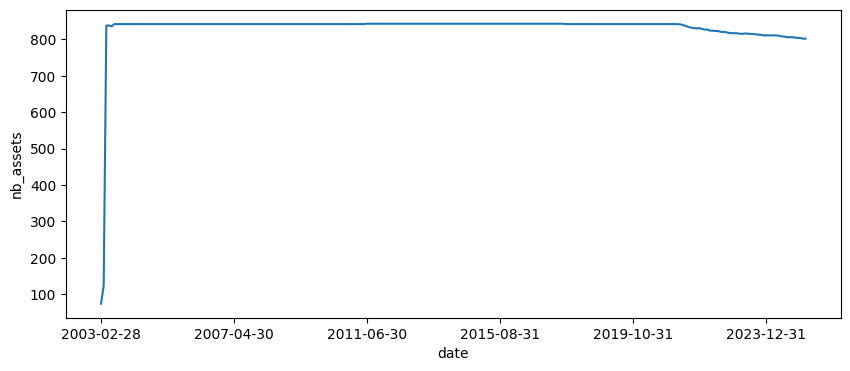
\includegraphics[width=0.7\linewidth]{files/6f8139a500c5d37e817276f15149f3db.png}

There are four immediate \textbf{labels} in the dataset: R1M, R3M, R6M and R12M, which correspond to the 1-month, 3-month, 6-month and 12-month future/forward returns of the stocks. The returns are \textbf{total returns}, that is, they incorporate potential \textbf{dividend} payments over the considered periods. This is a better proxy of financial gain compared to price returns only. We refer to the analysis of \citep{hartzmark2019dividend} for a study on the impact of decoupling price returns and dividends. These labels are located in the last 4 columns of the dataset. We provide their descriptive statistics below.

\begin{verbatim}
(data_ml[["R1M", "R3M", "R6M", "R12M"]]
    .describe()
    .T
    .loc[:, ["mean", "std", "min", "25%", "50%", "75%", "max"]]
    .round(3))
\end{verbatim}

\bigskip\noindent
\begin{tabular}{p{\dimexpr 0.125\linewidth-2\tabcolsep}p{\dimexpr 0.125\linewidth-2\tabcolsep}p{\dimexpr 0.125\linewidth-2\tabcolsep}p{\dimexpr 0.125\linewidth-2\tabcolsep}p{\dimexpr 0.125\linewidth-2\tabcolsep}p{\dimexpr 0.125\linewidth-2\tabcolsep}p{\dimexpr 0.125\linewidth-2\tabcolsep}p{\dimexpr 0.125\linewidth-2\tabcolsep}}
\toprule
 & mean & std & min & 25\% & 50\% & 75\% & max \\
\hline
R1M & 0.013 & 0.099 & -0.742 & -0.039 & 0.011 & 0.061 & 2.809 \\
\hline
R3M & 0.038 & 0.169 & -0.879 & -0.054 & 0.033 & 0.121 & 3.289 \\
\hline
R6M & 0.077 & 0.253 & -0.916 & -0.061 & 0.063 & 0.190 & 5.932 \\
\hline
R12M & 0.150 & 0.376 & -0.962 & -0.063 & 0.114 & 0.307 & 6.543 \\
\hline
\bottomrule
\end{tabular}

\bigskip

In anticipation for future models, we keep the name of the predictors in memory. In addition, we also keep a much shorter list of predictors.

\begin{verbatim}
features=list(data_ml.iloc[:,3:125].columns)
# Keep the feature's column names (hard-coded, beware!)
features_short =["Div_yld", "EPS", "size_avg_252d",
                 "mom_252", "OCF_Growth_1Y", "PB", "vol_252"]
\end{verbatim}

The predictors have been uniformized, that is, for any given feature and time point, the distribution is uniform. Imputation has also been performed, whereby any missing point is assigned the value 0.5. Below, we represent the distribution of dividend yield values, with all imputed values removed. Given roughly 800 stocks, the graph below cannot display a perfect rectangle.

\begin{verbatim}
data_ml.query('Div_yld != 0.5')['Div_yld'].hist(bins=100)
# using the hist
plt.ylabel('count')
\end{verbatim}

\begin{verbatim}
Text(0, 0.5, 'count')
\end{verbatim}

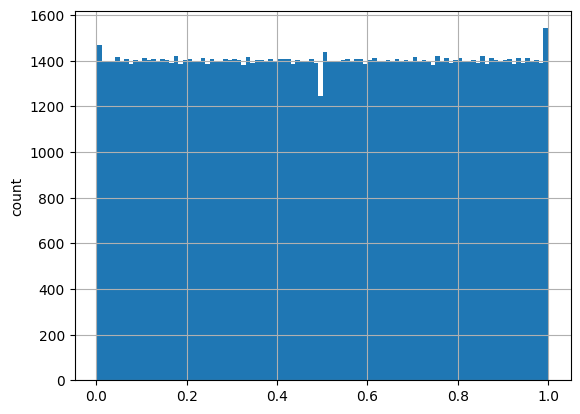
\includegraphics[width=0.7\linewidth]{files/ff5d1e41b539ab146eae15cf70c2a93c.png}

The original labels (future returns) are numerical and will be used for regression exercises, that is, when the objective is to predict a scalar real number. Sometimes, the exercises can be different and the purpose may be to forecast categories (also called classes), like ``buy'', ``hold'' or ``sell''. In order to be able to perform this type of classification analysis, we create additional labels that are categorical.

\begin{verbatim}
import numpy as np
df_median=[]  #creating empty placeholder for temporary dataframe
df=[]         #creating empty placeholder for temporary dataframe
df_median=data_ml[['date','R1M','R12M']].groupby(
    ['date']).median() # computings medians for both labels at each date
df_median.rename(
    columns={"R1M": "R1M_median",
             "R12M": "R12M_median"},inplace=True)
df = pd.merge(data_ml,df_median,how='left', on=['date'])
# join the dataframes
data_ml['R1M_C'] = np.where( # Create the categorical labels
    df['R1M'] > df['R1M_median'], 1.0, 0.0)
data_ml['R12M_C'] = np.where( # Create the categorical labels
    df['R12M'] > df['R12M_median'], 1.0, 0.0)
\end{verbatim}

The new labels are binary: they are equal to 1 (true) if the original return is above that of the median return over the considered period and to 0 (false) if not. Hence, at each point in time, half of the sample has a label equal to zero and the other half to one: some stocks overperform and others underperform.

In machine learning, models are estimated on one portion of data (training set) and then tested on another portion of the data (testing set) to assess their quality. We split our sample accordingly.

\begin{verbatim}
separation_date = "2017-01-15"
idx_train=data_ml.index[(data_ml['date']< separation_date)].tolist()
idx_test=data_ml.index[(data_ml['date']>= separation_date)].tolist()
\end{verbatim}

We also keep in memory a few key variables, like the list of asset identifiers and a rectangular version of returns. For simplicity, in the computation of the latter, we shrink the investment universe to keep only the stocks for which we have the maximum number of points. We provide a snapshot of the corresponding matrix.

\begin{verbatim}
stock_ids_short=[]   # empty placeholder for temporary dataframe
stock_days=[]        # empty placeholder for temporary dataframe
stock_ids=data_ml['fsym_id'].unique() # A list of all stock_ids
stock_days=data_ml[['date','fsym_id']].groupby(
    ['fsym_id']).count().reset_index() # compute nbr data points/stock
stock_ids_short=stock_days.loc[
    stock_days['date'] == (stock_days['date'].max())]
# Stocks with full data
stock_ids_short=stock_ids_short['fsym_id'].unique()
# in order to get a list
is_stock_ids_short=data_ml['fsym_id'].isin(stock_ids_short)
returns=data_ml[is_stock_ids_short].pivot(
    index='date',columns='fsym_id',values='R1M') # returns matrix
returns.iloc[0:5,0:5]
\end{verbatim}

\bigskip\noindent
\begin{tabular}{p{\dimexpr 0.167\linewidth-2\tabcolsep}p{\dimexpr 0.167\linewidth-2\tabcolsep}p{\dimexpr 0.167\linewidth-2\tabcolsep}p{\dimexpr 0.167\linewidth-2\tabcolsep}p{\dimexpr 0.167\linewidth-2\tabcolsep}p{\dimexpr 0.167\linewidth-2\tabcolsep}}
\toprule
fsym\_id & BV3N5V-R & BZPTB8-R & CHKL7S-R & CPCV0Y-R & CSMTMQ-R \\
\hline
date &  &  &  &  &  \\
\hline
2003-02-28 & -0.035187 & -0.026348 & 0.135182 & 0.034763 & -0.000831 \\
\hline
2003-03-31 & 0.098823 & -0.063574 & 0.038677 & 0.043919 & 0.084473 \\
\hline
2003-04-30 & 0.092791 & 0.187156 & 0.075814 & 0.141857 & 0.082452 \\
\hline
2003-05-31 & 0.061398 & 0.098532 & -0.037138 & 0.260852 & -0.065874 \\
\hline
2003-06-30 & 0.137763 & 0.027084 & 0.016328 & 0.010442 & 0.021819 \\
\hline
\bottomrule
\end{tabular}

\bigskip

\subsection{Introduction}

Conclusions often echo introductions. This chapter was completed at the very end of the writing of the book. It outlines principles and ideas that are probably more relevant than the sum of technical details covered subsequently. When stuck with disappointing results, we advise the reader to take a step away from the algorithm and come back to this section to get a broader perspective of some of the issues in predictive modelling.

\subsubsection{Context}

The blossoming of machine learning in factor investing has it source at the confluence of three favorable developments: data availability, computational capacity, and economic groundings.

First, the \textbf{data}. Nowadays, classical providers, such as Bloomberg and Reuters have seen their playing field invaded by niche players and aggregation platforms. In addition, high-frequency data and derivative quotes have become mainstream. Hence, firm-specific attributes are easy and often cheap to compile. This means that the size of $\mathbf{X}$ in Equation \ref{superv} below is was already sufficiently large in 2020 (first edition of the book) to be plugged into ML algorithms. The order of magnitude (in 2027, it has not changed much from 2019 in fact) that can be reached is the following:

\begin{itemize}
\item a few hundred monthly observations (a handful decades)
\item over several thousand stocks (US listed at least)
\item covering a several hundred attributes (sometimes a few thousand, but with possible colinearity).
\end{itemize}

This implies datasets of dozens of millions of points or more. While it is a reasonably high figure, we highlight that the chronological depth is probably the weak point and will remain so for decades to come because accounting figures are only released on a quarterly basis. This can somewhat be alleviated when generating synthetic data, though the efficiency of such strategy remains to be demonstrated. Needless to say that this drawback does not hold for high-frequency strategies that rely on intraday data (out of the scope of the present monograph).

Second, \textbf{computational power}, both through hardware and software. Storage and processing speed are not technical hurdles anymore and models can even be run on the cloud thanks to services hosted by major actors (Amazon, Microsoft, IBM and Google) and by smaller players (Rackspace, Techila). On the software side, open source has become the norm, funded by corporations (TensorFlow \& Keras by Google, Pytorch by META/Facebook, h2o, etc.), universities (Scikit-Learn by INRIA, NLPCore by Stanford, NLTK by UPenn) and small groups of researchers (caret, xgboost, catboost, lightGBM, tidymodels to list but a pair of frameworks). Consequently, ML is no longer the private turf of a handful of expert computer scientists, but is on the contrary \textbf{accessible} to anyone willing to learn and code. Moreover, with the advent of Large Languages Models, coding has never been easier.

Finally, \textbf{economic framing}. Machine learning applications in finance were initially introduced by computer scientists and information system experts (e.g., \citep{braun1987predicting}, \citep{white1988economic}) and exploited shortly after by academics in financial economics (\citep{bansal1993no}), and hedge funds (see, e.g., \citep{zuckerman2019man}). Nonlinear relationships then became more mainstream in asset pricing (\citep{freeman1992nonlinear}, \citep{bansal1993new}). These contributions started to pave the way for the more brute-force approaches that have blossomed since the 2010 decade and which are mentioned throughout the book.

In the synthetic proposal of \citep{arnott2019backtesting}, the first piece of advice is to rely on a model that makes sense economically. We agree with this stance, and the only assumption that we make in this book is that future returns depend on firm characteristics. The relationship between these features and performance is largely unknown and probably time-varying. This is why ML can be useful: to detect some hidden patterns beyond the documented asset pricing anomalies. Moreover, dynamic training allows to adapt to changing market conditions.

\subsubsection{Portfolio construction: the workflow}

Building successful portfolio strategies requires many steps. This book covers many of them but focuses predominantly on the prediction part. Indeed, allocating to assets most of the time requires to make bets and thus to presage and foresee which ones will do well and which ones will not. In this book, we mostly resort to supervised learning to forecast returns in the cross-section. The baseline equation in supervised learning,

\begin{equation}
\label{superv}
\mathbf{y}=f(\mathbf{X})+\mathbf{\epsilon},
\end{equation}

is translated in financial terms as

\begin{equation}
\label{superv_return}
\mathbf{r}_{t+1,n}=f(\mathbf{x}_{t,n})+\mathbf{\epsilon}_{t+1,n},
\end{equation}

where $f(\mathbf{x}_{t,n})$ can be viewed as the \textbf{expected return} for time $t+1$ computed at time $t$, that is, $\mathbb{E}_t[r_{t+1,n}]$. Note that the model is \textbf{common to all assets} ($f$ is not indexed by  $n$), thus it shares similarity with panel approaches.

Building accurate predictions requires to pay attention to \textbf{all} terms in the above equation. Chronologically, the first step is to gather data and to process it (see Chapter 4). To the best of our knowledge, the only consensus is that, on the $\textbf{x}$ side, the features should include classical predictors reported in the literature: market capitalization, accounting ratios, risk measures, momentum proxies (see Chapter 3). For the dependent variable, many researchers and practitioners work with monthly returns, but other maturities may perform better out-of-sample.

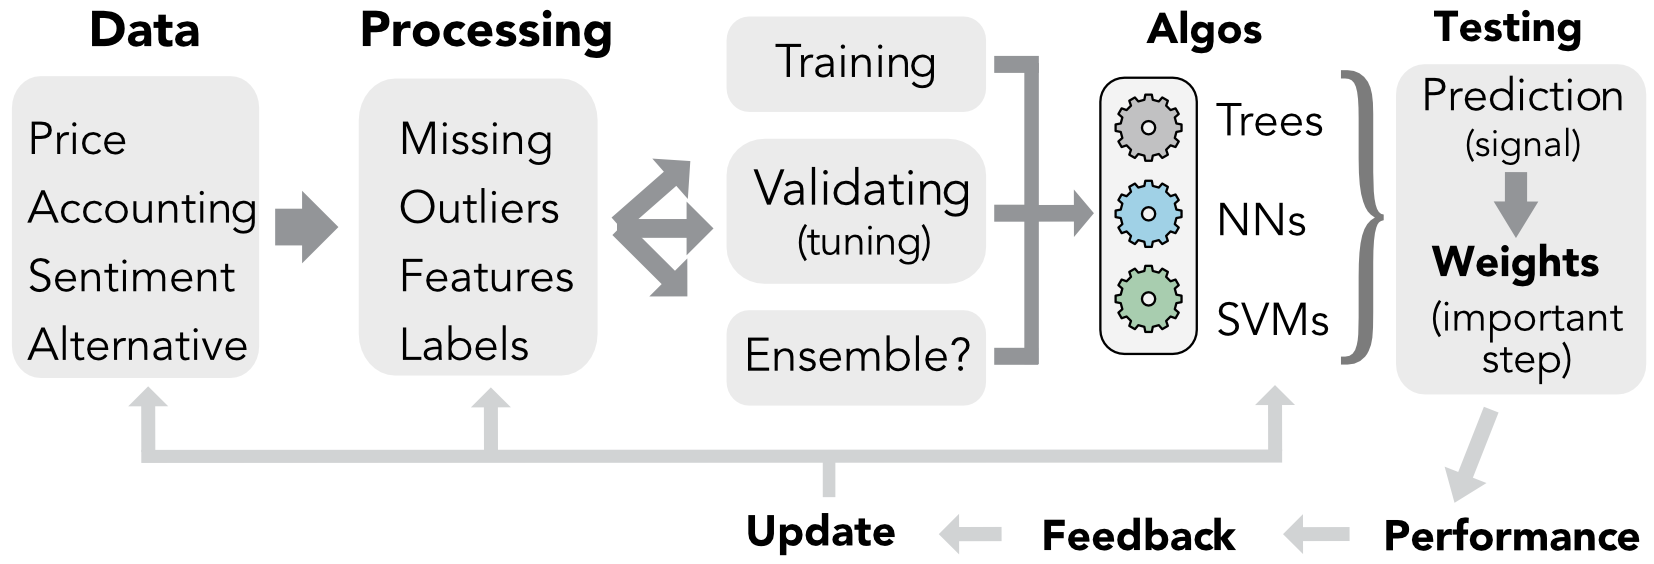
\includegraphics[width=0.7\linewidth]{files/scheme2_big-1e5ed17e728c0d450ddca5c5b6fa11ce.png}


Simplified workflow in ML-based portfolio construction.

\subsubsection{Machine Learning is no magic wand}

By definition, the curse of predictions is that they rely on \textbf{past} data to infer patterns about \textbf{subsequent} fluctuations. The more or less explicit hope of any forecaster is that the past will turn out to be a good approximation of the future. Needless to say, this is a pious wish; in general, predictions fare badly. Surprisingly, this does not depend much on the sophistication of the econometric tool. In fact, heuristic guesses are often hard to beat.

To illustrate this sad truth, the baseline algorithms that we detail in Chapters 5 to 7 yield at best mediocre results. This is done \textbf{on purpose}. This forces the reader to understand that blindly feeding data and parameters to a coded function will seldom suffice to reach satisfactory out-of-sample accuracy.

In machine learning, models are estimated on one portion of data (\textbf{training set}) and then tested on another portion of the data (\textbf{testing set}) to assess their quality. We split our sample accordingly.

Below, we sum up some key points that we have learned through our exploratory journey in financial ML.

\begin{itemize}
\item The first point is that \textbf{causality} is key. If one is able to identify $X \rightarrow y$, where $y$ are expected returns, then the problem is solved. Unfortunately, causality is incredibly hard to uncover.
\item Thus, researchers have most of the time to make do with simple \textbf{correlation} patterns, which are far less informative and robust.
\item Relatedly, financial datasets are extremely noisy. It is a daunting task to \textbf{extract signals} out of them. \textbf{No-arbitrage} reasonings imply that if a simple pattern yielded durable profits, it would mechanically and rapidly vanish.
\item The no-free lunch theorem of \citep{wolpert1992connection} imposes that the analyst formulates views on the model. This is why economic or \textbf{econometric framing} is key. The assumptions and choices that are made regarding both the dependent variables and the explanatory features are decisive. As a corollary, data is key. The inputs given to the models are probably much more important than the choice of the model itself.
\item To maximize out-of-sample efficiency, the right question is probably to paraphrase Jeff Bezos: what's not going to change? \textbf{Persistent} series are more likely to unveil enduring patterns.
\item Everybody makes mistakes. Errors in loops or variable indexing are part of the journey. What matters is to \textbf{learn} from those lapses.
\end{itemize}

To conclude, we remind the reader of this obvious truth: nothing will ever replace \textbf{practice}. Gathering and cleaning data, coding backtests, tuning ML models, testing weighting schemes, debugging, starting all over again: these are all absolutely indispensable steps and tasks that must be repeated indefinitely. There is no sustitute to experience.

\subsection{Factor investing and asset pricing anomalies}

Asset pricing anomalies are the foundations of \textbf{factor investing}. In this chapter, probably the longest in the book, our aim is twofold:

\begin{itemize}
\item first, to present simple ideas and concepts: basic factor models and common empirical facts (time-varying nature of returns and risk premia);
\item second, provide the reader with lists of articles that go much deeper to stimulate and satisfy curiosity. Indeed, the literature on anomalies encompasses thousands of research articles and it is impossible to do it justice in one single chapter.
\end{itemize}

The purpose of this chapter is thus not to provide a full treatment of the many topics related to factor investing. Rather, it is intended to give a broad overview and cover the essential themes so that the reader is guided towards the relevant references. As such, it can serve as a short, non-exhaustive, review of the literature. The subject of factor modelling in finance is incredibly vast and the number of papers dedicated to it is substantial and still rapidly increasing, even as of 2026, when most of the chapters were updated and partly re-written.

The universe of peer-reviewed financial journals can be split in two:

\begin{itemize}
\item The first kind journals are the \textbf{academic journals}. Their articles are mostly written by professors, and the audience consists mostly of scholars. The articles are long and often technical. Prominent examples are the \href{https://onlinelibrary.wiley.com/journal/15406261}{\textit{Journal of Finance}}, the \href{https://academic.oup.com/rfs}{\textit{Review of Financial Studies}} and the \href{https://www.sciencedirect.com/journal/journal-of-financial-economics}{\textit{Journal of Financial Economics}}.
\item The second type is more \textbf{practitioner}-orientated. The papers are shorter, easier to read, and target finance professionals predominantly. Two emblematic examples are the \href{https://www.pm-research.com/content/iijpormgmt}{\textit{Journal of Portfolio Management}} and the \href{https://www.tandfonline.com/journals/ufaj20}{\textit{Financial Analysts Journal}}.
\end{itemize}

This chapter reviews and mentions articles published mostly in the first family of journals. Sometimes, we nevertheless also cite working papers or ideas that have originated from the industry.

Beyond academic articles, several monographs are already dedicated to the topic of style allocation (a synonym of factor investing used for instance in theoretical articles \cite{barberis2003style} or practitioner papers \cite{asness2015investing}). To cite but a few, we mention:

\begin{itemize}
\item \cite{ilmanen2011expected}: an exhaustive excursion into risk premia, across many asset classes, with a large spectrum of descriptive statistics (across factors and periods),
\item \cite{ang2014asset}: covers factor investing with a strong focus on the money management industry,
\item \cite{bali2016empirical}: very complete book on the cross-section of signals with statistical analyses (univariate metrics, correlations, persistence, etc.),
\item \cite{jurczenko2017factor}: a tour on various topics given by field experts (factor purity, predictability, selection versus weighting, factor timing, etc.).
\item \cite{zhang2024navigating}: a more recent treatment of various topics in the fields, including, e.g., quantamental views and behavioral finance.
\end{itemize}

Finally, we can mention a few wide-scope and survey papers on this topic: \cite{goyal2012empirical}, \cite{cazalet2014facts}, \cite{baz2015dissecting}, \cite{giglio2022factor} and \cite{shi2025econometrics}.

\subsubsection{Introduction: why factors?}

The topic of factor investing, though a decades-old academic theme, has gained traction concurrently with the rise of equity traded funds (ETFs) as vectors of investment (see Figure~\ref{fig-etf_aum_evolution} below). Both have gathered momentum in the 2010 decade. Not so surprisingly, the feedback loop between practical financial engineering and academic research has stimulated both sides in a mutually beneficial manner. Practitioners rely on key scholarly findings (e.g., on asset pricing anomalies) while researchers dig deeper into pragmatic topics (e.g., factor exposure or transaction costs). Recently, researchers have also tried to quantify and qualify the impact of factor indices on financial markets. For instance, \cite{krkoska2019herding} analyze herding behaviors while \cite{cong2019rise} show that the introduction of composite securities increases volatility and cross-asset correlations. \cite{demiguel2019crowding} find that the increase competition in the factor space \textit{may} increase profits due to the netting of trades across factors - but this is far from guaranteed, too.

\begin{figure}[!htbp]
\centering
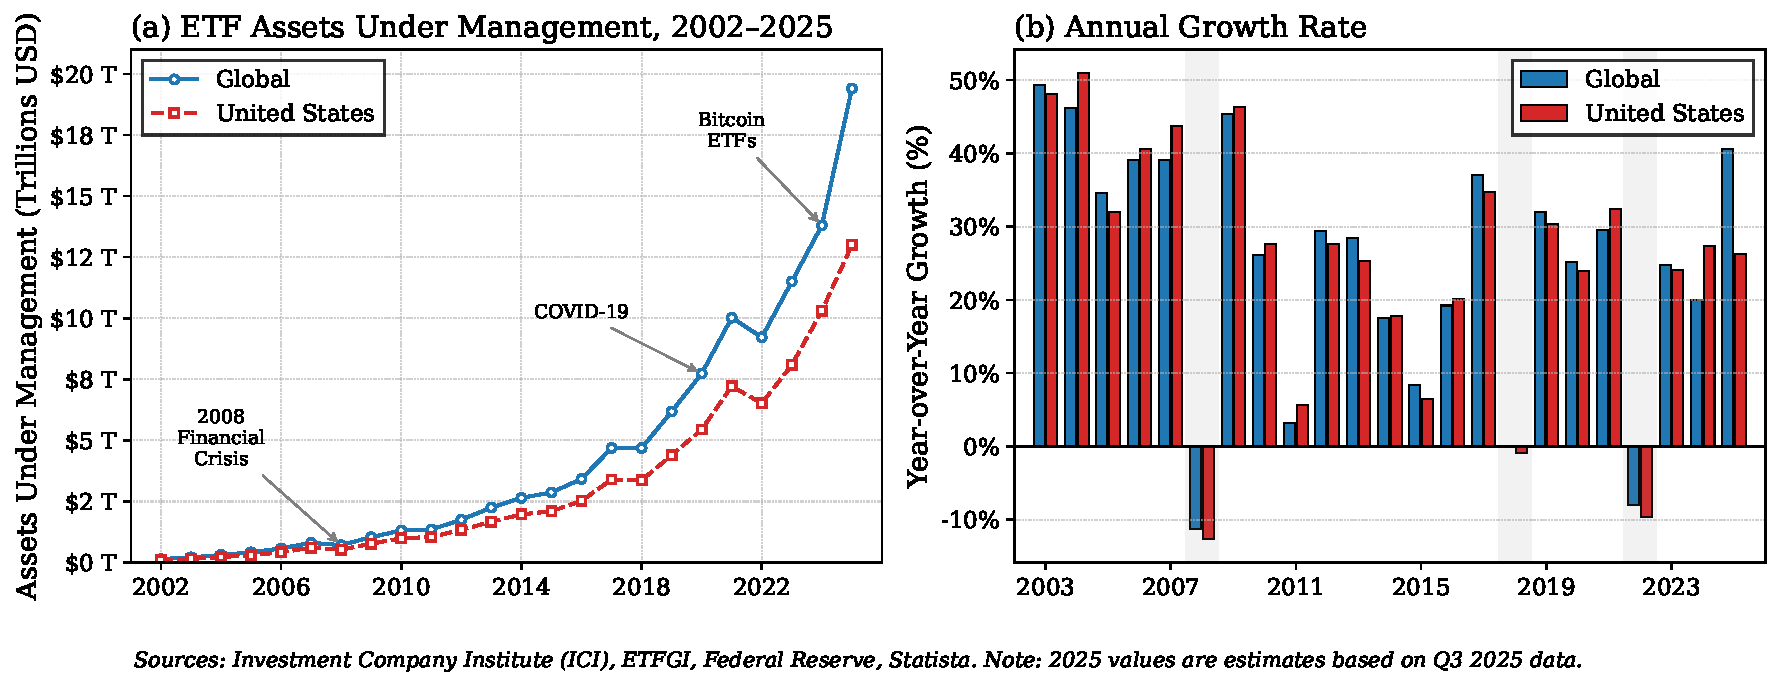
\includegraphics[width=0.7\linewidth]{files/etf_aum_evolution-60736420a5e4cc0584bd995a7cfb32ea.pdf}
\caption[]{Evolution of the ETF market (assets under management).}
\label{fig-etf_aum_evolution}
\end{figure}

The core aim of factor models is to understand the \textbf{drivers of asset prices and their changes}. Broadly speaking, the rationale behind factor investing is that the financial performance of firms depends on factors, whether they be latent and unobservable, or related to intrinsic characteristics (like accounting ratios for instance, past performance, or even sustainability metrics). Indeed, as \cite{cochrane2011presidential} frames it, the first essential question is \textit{which characteristics really provide independent information about average returns?} Answering this question helps understand the cross-section of returns and may open the door to their prediction.

Theoretically, linear factor models can be viewed as special cases of the arbitrage pricing theory (APT) of \cite{ross1976arbitrage}, which assumes that the return of an asset $n$ can be modelled as a linear combination of underlying factors $f_k$:

\begin{equation}
\label{apt}
r_{t,n}= \alpha_n+\sum_{k=1}^K\beta_{n,k}f_{t,k}+\epsilon_{t,n},
\end{equation}

where the usual econometric constraints on linear models hold: $\mathbb{E}[\epsilon_{t,n}]=0$, $\text{cov}(\epsilon_{t,n},\epsilon_{t,m})=0$ for $n\neq m$ and $\text{cov}(\textbf{f}_n,\boldsymbol{\epsilon}_n)=0$. If such factors do exist, then they are in contradiction with the cornerstone model in asset pricing: the capital asset pricing model (CAPM) of \cite{sharpe1964capital}, \cite{lintner1965valuation} and \cite{mossin1966equilibrium}. Indeed, according to the CAPM, the only driver of returns should be the market portfolio. This explains why factors are also called `\textit{anomalies}'.

One robust theoretical foundation for anomalies stems from the recent demand-based pricing literature initiated by \cite{koijen2019demand}. Therein, the authors show that if moments of returns are linked to firms characteristics, then optimal portfolios, too, are naturally tied to these characteristics. Hence, upon market clearing, returns should also be driven by firm attributes (see also the work of \cite{van2026flow} related to ESG preferences). In short, the model assumes:
\begin{equation}
\text{demand}(\text{price},\text{other characteristics}) = \text{supply}(\text{orthogonal motives}) ,
\end{equation}
and hence price changes are linked to the characteristics. Now, as \cite{coqueret2022characteristics} shows, if preferences are logarithmic, as in \cite{koijen2019demand}, then it is possible to derive that returns depend on these characteristics, as well as on \textit{relative changes} in the characteristics (this is sometimes referred to as \textit{characteristic momentum}). If demand is linear in firm attributes, then returns, too, become linear in these attributes (and their changes).

In the end, we obtain a (predictive) panel model of the form:
\begin{equation}
r_{t+1,n}=g(\textbf{c}_{t,n}, \textbf{c}_{t-1,n}) + e_{t+1, n}.
\end{equation}
An interesting question pertains to the relative importance of the error term, $e_{t+1,n}$. This is sometimes referred to as the \textit{latent demand}, i.e., the portion of demand (or, in the above equation, of returns) that cannot be explained by the characteristics. \cite{koijen2019demand} find that it is in fact sizeable, accounting for at least of 80\% of variation in demands. A growing body of work has since refined and challenged this framework; we dedicate a full section below (Section 3.5) to recent theoretical foundations, identification issues, and extensions to richer preference structures.

Empirical evidence of asset pricing anomalies has accumulated since the dual publication of \cite{fama1992cross} and \cite{fama1993common}. This seminal work has paved the way for a blossoming stream of literature that has its meta-studies (e.g., \cite{green2013supraview}, \cite{harvey2016and} and \cite{mclean2016does}). The regression in Equation \ref{apt} can be evaluated once (unconditionally) or sequentially over different time frames. In the latter case, the parameters (coefficient estimates) change and the models are thus called conditional (we refer to \cite{ang2012testing} and to \cite{cooper2018new} for recent results on this topic as well as for a detailed review on the related research). Conditional models are more flexible because they acknowledge that the drivers of asset prices may not be constant, which seems like a reasonable postulate.

\subsubsection{The factor zoo}

\paragraph{The canonical factors}

The construction of so-called factors follows the same lines as above. Portfolios are based on one characteristic and the factor is a long-short ensemble of one extreme portfolio minus the opposite extreme (small minus large for the size factor or high book-to-market ratio minus low book-to-market ratio for the value factor). Sometimes, subtleties include forming bivariate sorts (e.g., using firm size) and aggregating several portfolios together, as in the original contribution of \cite{fama1993common}. The most common factors are listed below, along with a few references. We refer to the books listed at the beginning of the chapter for a more exhaustive treatment of factor idiosyncrasies. For most anomalies, theoretical justifications have been brought forward, whether risk-based or behavioral. We list the most frequently cited factors below:

\begin{itemize}
\item Size (\textbf{SMB} = small firms minus large firms): \cite{banz1981relationship}, \cite{fama1992cross}, \cite{fama1993common}, \cite{van2011size}, \cite{asness2018size} and \cite{astakhov2019firm}.
\item Value (\textbf{HML} = high minus low: undervalued minus growth firms): \cite{fama1992cross}, \cite{fama1993common}, \cite{asness2013devil}, and \cite{asness2013value}.
\item Momentum (\textbf{WML} = winners minus losers): \cite{jegadeesh1993returns}, \cite{carhart1997persistence} and \cite{asness2013value}. The winners are the assets that have experienced the highest returns over the last year (sometimes the computation of the return is truncated to omit the last month). Cross-sectional momentum is linked, but not equivalent, to time series momentum (trend following), see e.g., \cite{moskowitz2012time} and \cite{lemperiere2014two}. Momentum is also related to contrarian movements that occur both at higher and lower frequencies (short-term and long-term reversals), see \cite{luo2020momentum}.
\item Profitability (\textbf{RMW} = robust minus weak profits): \cite{fama2015five}, \cite{bouchaud2019sticky}. In the former reference, profitability is measured as (revenues - (cost and expenses))/equity.
\item Investment (\textbf{CMA} = conservative minus aggressive): \cite{fama2015five}, \cite{hou2015digesting}. Investment is measured via the growth of total assets (divided by total assets). Aggressive firms are those that experience the largest growth in assets.
\item Low risk (sometimes, \textbf{BAB} = betting against beta): \cite{ang2006cross}, \cite{baker2011benchmarks}, \cite{frazzini2014betting}, \cite{boloorforoosh2019beta}, \cite{baker2019leverage} and \cite{asness2020betting}. In this case, the computation of risk changes from one article to the other (simple volatility, market beta, idiosyncratic volatility, etc.).
\item Green (\textbf{GMB} = green minus brown): \cite{pastor2021sustainable}, \cite{lioui2022chasing}, see also \cite{coqueret2022perspectives} for an early review on sustainable equity investing. This subject, the greenium, has become so vast that it is impossible to review thoroughly.
\end{itemize}

With the notable exception of the low risk premium and the greenium, the most mainstream anomalies are kept and updated in the data library of \href{https://mba.tuck.dartmouth.edu/pages/faculty/ken.french/data\_library.html}{Kenneth French}. Of course, the computation of the factors follows a particular set of rules, but they are generally accepted in the academic sphere. Another source of data is the \href{https://www.aqr.com/Insights/Datasets}{AQR repository}. Finally, one recent and very popular repository is that of the \href{https://www.openassetpricing.com/}{Open Source Asset Pricing} project that regularly updates the work of \cite{chen2021open}.

A recent survey by \cite{welch2026assessing} offers a rare view of academic consensus on factor premia. Out of 254 researchers polled at top US universities, the four factors with the broadest support for positive expected returns are momentum, profitability, value and market beta. Only market beta and value are widely classified as genuine risk factors; the others are viewed as behavioral anomalies or market imperfections.

In the dataset we use for the book, we proxy the value anomaly not with the book-to-market ratio but with the price-to-book ratio (the book value is located in the denominator). As is shown in \cite{asness2013devil}, the choice (and timing) of the variable for value can have sizable effects.

First, let's load the relevant libraries.

\begin{verbatim}
# Required libraries
import pandas as pd
import numpy as np
import matplotlib.pyplot as plt
import seaborn as sns
from datetime import datetime
import statsmodels.api as sm
from myst_nb import glue
from statsmodels.graphics.tsaplots import plot_acf

# Display settings
pd.set_option('display.max_columns', 10)
plt.style.use('seaborn-v0_8-whitegrid')

# Building the data
from data_build import generate_data
from data_build import get_significance
from data_build import compute_size_portfolios
data_ml, features, features_short, returns, stock_ids, stock_ids_short = generate_data()
\end{verbatim}

Below, we import data from Ken French's data library. We will use it later on in the chapter.

\begin{figure}
\centering
\begin{verbatim}
min_date = pd.to_datetime('1963-07-01')
max_date = pd.to_datetime('2024-03-01')
ff_url = "https://mba.tuck.dartmouth.edu/pages/faculty/ken.french/ftp"
ff_url += "/F-F_Research_Data_5_Factors_2x3_CSV.zip"
# Create the download url
df_ff = pd.read_csv(ff_url, sep=',', skiprows=3, quotechar='"')
df_ff.rename(columns = {'Unnamed: 0':'date'},
             inplace = True) # renaming for clarity
df_ff.rename(columns = {'Mkt-RF':'MKT_RF'},
             inplace = True) # renaming for clarity
df_ff = df_ff.iloc[0:743, :]    
df_ff['date'] = pd.to_datetime(df_ff['date'], format='%Y%m')  
df_ff["date"] = df_ff["date"] + pd.DateOffset(months=1) - pd.Timedelta(days=1)       
df_ff[['MKT_RF','SMB','HML','RMW','CMA','RF']] = df_ff[['MKT_RF','SMB','HML','RMW','CMA','RF']].apply(pd.to_numeric)
df_ff[['MKT_RF','SMB','HML','RMW','CMA','RF']]=df_ff[
    ['MKT_RF','SMB','HML','RMW','CMA','RF']].values/100.0 # Scale returns
idx_ff=df_ff.index[(df_ff['date']>=min_date)&(
    df_ff['date']<=max_date)].tolist()
FF_factors=df_ff.iloc[idx_ff].copy()
FF_factors.loc[:,'year']=FF_factors.date.astype(str).str[:4]
FF_factors.iloc[1:6,0:7].head()
\end{verbatim}
\caption[]{Snapshot of Fama-French factor returns. Source: Ken French library.

\begin{tabular}{p{\dimexpr 0.125\linewidth-2\tabcolsep}p{\dimexpr 0.125\linewidth-2\tabcolsep}p{\dimexpr 0.125\linewidth-2\tabcolsep}p{\dimexpr 0.125\linewidth-2\tabcolsep}p{\dimexpr 0.125\linewidth-2\tabcolsep}p{\dimexpr 0.125\linewidth-2\tabcolsep}p{\dimexpr 0.125\linewidth-2\tabcolsep}p{\dimexpr 0.125\linewidth-2\tabcolsep}}
\toprule
 & date & MKT\_RF & SMB & HML & RMW & CMA & RF \\
\hline
1 & 1963-08-31 & 0.0508 & -0.0080 & 0.0170 & 0.0040 & -0.0038 & 0.0025 \\
\hline
2 & 1963-09-30 & -0.0157 & -0.0043 & 0.0000 & -0.0078 & 0.0015 & 0.0027 \\
\hline
3 & 1963-10-31 & 0.0254 & -0.0134 & -0.0004 & 0.0279 & -0.0225 & 0.0029 \\
\hline
4 & 1963-11-30 & -0.0086 & -0.0085 & 0.0173 & -0.0043 & 0.0227 & 0.0027 \\
\hline
5 & 1963-12-31 & 0.0183 & -0.0189 & -0.0021 & 0.0012 & -0.0025 & 0.0029 \\
\hline
\bottomrule
\end{tabular}}
\label{fig-FF_returns}
\end{figure}

\paragraph{Theoretical foundations}

Posterior to the discovery of these stylized facts, some contributions have aimed at building theoretical models that capture these properties. Theorizing a posteriori is sometimes called HARKing (see \cite{kerr1998harking} and \cite{hollenbeck2017harking}). We cite a handful below:

\begin{itemize}
\item \textbf{size} and \textbf{value}: \cite{berk1999optimal}, \cite{daniel2001overconfidence}, \cite{barberis2003style}, \cite{gomes2003equilibrium}, \cite{carlson2004corporate}, \cite{arnott2014can};
\item \textbf{momentum}: \cite{johnson2002rational}, \cite{grinblatt2005prospect}, \cite{vayanos2013institutional}, \cite{choi2014momentum}, \cite{li2018explaining} (with value, too).
\end{itemize}

In addition, bridges have also been built between risk-based factor representations and behavioural theories. We refer essentially to \cite{barberis2016prospect} and \cite{daniel2019short} and the references therein.

The individual attributes of investors who allocate towards particular factors is a blossoming topic. We list a few references below, even though they somewhat lie out of the scope of this book. \cite{betermier2017value} show that value investors are older, wealthier and face lower income risk compared to growth investors who are those in the best position to take financial risks. The study \cite{cronqvist2015value} leads to different conclusions: it finds that the propensity to invest in value versus growth assets has roots in genetics and in life events (the latter effect being confirmed in \cite{cocco2019evidence}, and the former being further detailed in a more general context in \cite{cronqvist2015value}). Psychological traits can also explain some factors: when agents extrapolate, they are likely to fuel momentum (this topic is thoroughly reviewed in \cite{barberis2018psychology}). Micro- and macro-economic consequences of these preferences are detailed in \cite{bhamra2019does}. To conclude this paragraph, we mention that theoretical models have also been proposed that link agents' preferences and beliefs (via prospect theory) to market anomalies (see for instance \cite{du2020deep}).

\paragraph{Time-varying premia and anomaly dynamics}

While these factors (i.e., long-short portfolios) exhibit time-varying risk premia and are magnified by corporate news and announcements \citep{engelberg2018anomalies}, it is \textit{roughly} accepted that they deliver positive returns over long horizons (this has been challegnged by \cite{smith2022have}). We refer to \cite{gagliardini2016time} and to the survey \cite{gagliardini2019estimation}, as well as to the related bibliography for technical details on estimation procedures of risk premia and the corresponding empirical results. A large sample study that documents regime changes in factor premia was also carried out by \cite{ilmanen2019factor}. Moreover, the predictability of returns is also time-varying (as documented in \cite{farmer2019pockets}, \cite{tsiakas2020equity} and \cite{liu2020can}), and estimation methods can be improved \citep{johnson2019fresh}.

In Figure~\ref{fig-return_anomalies}, we plot the average monthly return aggregated over each calendar year for five common factors and the risk-free rate. The risk free rate (which is not a factor per se) is the logically most stable, while the market factor (aggregate market returns minus the risk-free rate) is the most volatile. This makes sense because it is the only long equity factor among the five series, hence the short leg cannot hedge the long one.

\begin{figure}[!htbp]
\centering
\begin{verbatim}
# Plot average annual returns for Fama-French factors
FF_annual = FF_factors.copy()
FF_annual['year'] = FF_annual['date'].dt.year

# Melt to long format
factors_to_plot = ['MKT_RF', 'SMB', 'HML', 'RMW', 'CMA', 'RF']
FF_long = FF_annual.melt(
    id_vars=['year'], 
    value_vars=factors_to_plot,
    var_name='factor', 
    value_name='return'
)

# Compute annual average
FF_avg = FF_long.groupby(['year', 'factor'])['return'].mean().reset_index()

# Plot
fig, ax = plt.subplots(figsize=(12, 5))
for factor in factors_to_plot:
    subset = FF_avg[FF_avg['factor'] == factor]
    ax.plot(subset['year'], subset['return'], label=factor)

ax.set_xlabel('Year')
ax.set_ylabel('Average Monthly Return')
ax.set_title('Average Returns of Common Anomalies')
ax.legend()
plt.tight_layout()
plt.show()
\end{verbatim}
\caption[]{Average returns of common anomalies plus the risk-free rate (1963-2024). Source: Ken French library.

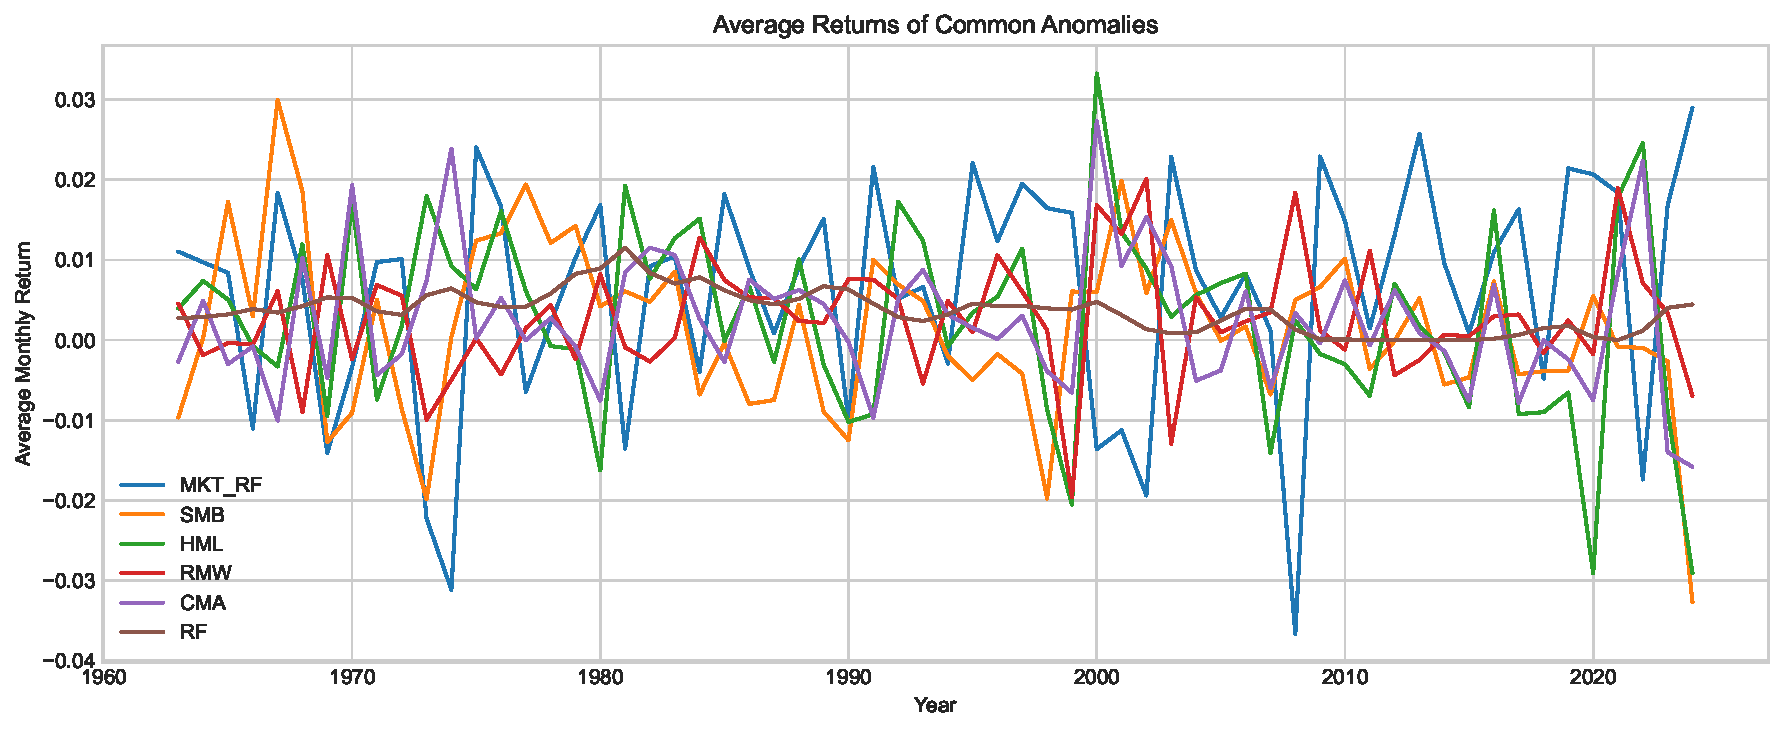
\includegraphics[width=0.7\linewidth]{files/a23234d5f4c4cb175bbe8bf2f89be511.pdf}}
\label{fig-return_anomalies}
\end{figure}

Beyond crowding and publication effects, anomalies also differ in their \textit{dynamic nature}. \cite{vanbinsbergen2023dynamic} classify anomalies into two types: \textit{build-up} anomalies (e.g., momentum, profitability) that exacerbate mispricing over time, and \textit{resolution} anomalies (e.g., value, size, investment) that correct it. This taxonomy has practical implications: build-up anomalies are driven by overreaction and may contribute to real capital misallocation, while resolution anomalies are self-correcting.

\paragraph{Fading anomalies and replicability}

Some researchers document fading anomalies because of publication: once the anomaly becomes public, agents invest in it, which pushes prices up and the anomaly disappears. \cite{mclean2016does} document this effect in the US but \cite{jacobs2019anomalies} find that all other countries experience sustained post-publication factor returns. With a different methodology, \cite{chen2020publication} introduce a publication bias adjustment for returns and the authors note that this (negative) adjustment is in fact rather small. \cite{penasse2018understanding} recommends the notion of \textit{alpha decay} to study the persistence or attenuation of anomalies.

The destruction of factor premia may be due to herding (\cite{krkoska2019herding}, \cite{volpati2020zooming}) and could be accelerated by the democratization of so-called smart-beta products (ETFs notably) that allow investors to directly invest in particular styles (value, low volatility, etc.). For a theoretical perspective on the attractivity of factor investing, we refer to \cite{jin2019drivers}. On the other hand, \cite{demiguel2019crowding} argue that the price impact of crowding in the smart-beta universe is mitigated by trading diversification stemming from external institutions that trade according to strategies outside this space (e.g., high frequency traders betting via order-book algorithms).

Finally, we highlight the need of replicability of factor premia and echo the critical editorial by \cite{harvey2019evaluation}. As is shown by \cite{linnainmaa2018history} and \cite{hou2019replicating}, many proclaimed factors are in fact very much data-dependent and often fail to deliver sustained profitability when the investment universe is altered or when the definition of variable changes \citep{asness2013devil}. Nevertheless, \cite{chen2020publication} and \cite{chen2021open} challenge the idea of low replicability, even if out-of-sample evaluation and transaction costs strongly curtail performance \citep{chen2020zeroing}. All in all, as \cite{chen2024does} argue, whether published anomalies fare better than pure data mining remains an open question.

A methodological contribution that sheds light on which characteristics truly matter is provided by \cite{seyfi2025essence}, who flips the standard approach: instead of sorting stocks by characteristics and measuring returns, the author sorts by realized returns and then identifies which characteristics best replicate those return-sorted portfolios out-of-sample. This ``reverse engineering'' approach theoretically comes closest to the unknown optimal sorting on SDF exposures and empirically finds that price-based characteristics and their interactions are the strongest predictors --- outperforming prominent ML methods.

Recent work has also tried to quantify how much capital must be deployed before a strategy's alpha disappears. \cite{davis2026erasing} find, for the value factor, that reallocating the full pool of growth fund assets under management into value would barely reduce the value premium, implying a strategy capacity in the trillions of dollars. A side effect they document is that flows intended to compress one strategy can mechanically inflate the alpha of another through overlapping holdings.

For ML strategies specifically, \cite{azevedo2025expected} show that publication effects, transaction costs and increased market liquidity together reduce average ML strategy performance by roughly 57\% relative to standard backtests. Sophisticated architectures such as LSTM networks remain profitable after these adjustments. \cite{alexander2024measuring} complement this with the Minimum Regime Performance, a lower bound on strategy robustness that captures how a strategy fares in its worst historical market regime. Their finding is sobering: quality is the only major factor with a positive minimum regime return.

Campbell Harvey and his co-authors, in a series of papers, tried to synthesize the early research on factors in \cite{harvey2016and}, \cite{harvey2017lucky} and \cite{harvey2017lucky}. This work underlines the need to set high bars for an anomaly to be called a `true' factor. Increasing thresholds for $p$-values is only a partial answer (critiqued in \cite{chen2020t}), as it is always possible to resort to data snooping in order to find an optimized strategy that will fail out-of-sample but that will deliver a $t$-statistic larger than three (or even four). \cite{harvey2017presidential} recommends to resort to a Bayesian approach which blends data-based significance with a prior into a so-called Bayesianized \textit{p}-value (see subsection below).

Following this work, researchers have continued to explore the richness of this zoo. \cite{bryzgalova2019spurious} propose a tractable Bayesian estimation of large-dimensional factor models and evaluate all possible combinations of more than 50 factors, yielding an incredibly large number of coefficients. This combined with a \cite{fama1973risk} procedure allows to distinguish between pervasive and superfluous factors. \cite{chordia2020anomalies} use simulations of 2 million trading strategies to estimate the rate of \textit{false discoveries}, that is, when a spurious factor is detected (type I error). They also advise to use thresholds for \textit{t}-statistics that are well above three. In a similar vein, \cite{harvey2019false} also underline that sometimes \textit{true} anomalies may be missed because of a one time \textit{t}-statistic that is too low (type II error).

The propensity of journals to publish positive results has led researchers to estimate the difference between reported returns and \textit{true} returns. \cite{chen2020limits} call this difference the \textit{publication bias} and estimate it as roughly 12\%. That is, if a published average return is 8\%, the actual value may in fact be closer to (1-12\%)*8\%=7\%. Qualitatively, this estimation of 12\% is smaller than the out-of-sample reduction in returns found in \cite{mclean2016does}.

\subsubsection{Detecting and testing anomalies}

\paragraph{Challenges}

Obviously, a crucial step is to be able to identify an anomaly and the complexity of this task should not be underestimated. Given the publication bias towards positive results (see, e.g., \cite{harvey2017presidential} in financial economics), researchers are often tempted to report partial results that are sometimes invalidated by further studies. The need for replication is therefore high and many findings have no tomorrow (\cite{linnainmaa2018history}, \cite{johannesson2020explanatory}), especially if transaction costs are taken into account (\cite{novy2015taxonomy}, \cite{patton2020you}, \cite{chen2020zeroing}). Nevertheless, as is demonstrated by \cite{chen2020limits}, $p$-hacking alone cannot account for all the anomalies documented in the literature. One way to reduce the risk of spurious detection is to increase the hurdles (often, the $t$-statistics) but the debate is still ongoing (\cite{harvey2016and}, \cite{chen2020t}), or to resort to multiple testing (\cite{harvey2019evaluation}, \cite{vincent2020investment}).

The remainder of this subsection was inspired from \cite{baker2017detecting} and \cite{harvey2017lucky}.

\paragraph{Simple portfolio sorts}

This is the most common procedure and the one used in \cite{fama1992cross}. The idea is simple. On one date,

\begin{enumerate}
\item rank firms according to a particular criterion (e.g., size, book-to-market ratio);
\item form $J\ge 2$ portfolios (i.e., homogeneous groups) consisting of the same number of stocks according to the ranking (usually, $J=2$, $J=3$, $J=5$ or $J=10$ portfolios are built, based on the median, terciles, quintiles or deciles of the criterion);
\item the weight of stocks inside the portfolio is either uniform (equal weights), or proportional to market capitalization (cap-weighted, in short);
\item at a future date (usually one month), report the returns of the portfolios. Then, iterate the procedure until the chronological end of the sample is reached.
\end{enumerate}

The outcome is a time series of portfolio returns $r_t^j$ for each grouping $j$. An anomaly is identified if the \textit{t}-test between the first ($j=1$) and the last group ($j=J$) unveils a significant difference in average returns. More robust tests are described in \cite{cattaneo2019characteristic}. A strong limitation of this approach is that the sorting criterion could have a non-monotonic impact on returns and a test based on the two extreme portfolios would not detect it. Several articles address this concern: \cite{patton2010monotonicity} and \cite{romano2013testing} for instance. Another concern is that these sorted portfolios may capture not only the priced risk associated with the characteristic but also some unpriced risk. \cite{daniel2020cross} show that it is possible to disentangle the two and make the most of altered sorted portfolios. We recall a lesser known fact: average returns from sorted long-short portfolios can be viewed as estimates from linear regressions without intercepts (see page 326 of \cite{fama1976foundations} and the Appendix of \cite{freyberger2020dissecting}).

Instead of focusing on only one criterion, it is possible to group assets according to more characteristics. The original paper \cite{fama1992cross} also combines market capitalization with book-to-market ratios. Each characteristic is divided into 10 buckets, which makes 100 portfolios in total. Beyond data availability, there is no upper bound on the number of features that can be included in the sorting process. In fact, some authors investigate more complex sorting algorithms that can manage a potentially large number of characteristics (see e.g., \cite{feng2019taming} and \cite{bryzgalova2019bayesian}).

In addition, we refer to \cite{ledoit2018efficient} for refinements that take into account the covariance structure of asset returns, and to \cite{cattaneo2019characteristic} for a theoretical study on the statistical properties of the sorting procedure (including theoretical links with regression-based approaches). Notably, the latter paper discusses the optimal number of portfolios and suggests that it is probably larger than the usual 10 often used in the literature.

More recently, \cite{hoechle2025generalized} propose a Generalized Portfolio Sorts (GPS) framework that nests all conventional sort variants but can additionally separate a characteristic's genuine predictive power from persistent firm-level heterogeneity (e.g., permanent differences across industries). Applying GPS to a large set of predictors, nearly half of the anomalies documented in the literature lose their statistical significance once this heterogeneity is accounted for: a rather sobering finding for factor-based strategies.

In a different direction, \cite{liu2026uncertainty} argue that the standard practice of sorting stocks by \textit{point predictions} discards valuable information about prediction uncertainty. They propose uncertainty-adjusted sorting, in which long positions are ranked by optimistic (upper-bound) predictions and short positions by pessimistic (lower-bound) ones. This approach systematically improves Sharpe ratios relative to standard sorts, with the gains concentrated in stocks for which prediction uncertainty is highest.

In the code and Figure~\ref{fig-size_factor} below, we compute the returns of size portfolios (equally weighted: above versus below the median capitalization). According to the size anomaly, the firms with below median market cap should earn higher returns on average. This is verified whenever the orange bar in the plot is above the blue one (it happens most of the time).

We first import the librairies used throughout the chapter.

\begin{verbatim}
# Required libraries
import pandas as pd
import numpy as np
import matplotlib.pyplot as plt
import seaborn as sns
from datetime import datetime
import statsmodels.api as sm
from myst_nb import glue
from statsmodels.graphics.tsaplots import plot_acf

# Display settings
pd.set_option('display.max_columns', 10)
plt.style.use('seaborn-v0_8-whitegrid')

# Building the data
from data_build import generate_data
from data_build import get_significance
from data_build import compute_size_portfolios
data_ml, features, features_short, returns, stock_ids, stock_ids_short = generate_data()
\end{verbatim}

Next, we compute and plot the annual returns of the \textbf{size anomaly} (small-minus-big).

\begin{figure}[!htbp]
\centering
\begin{verbatim}
size_returns = compute_size_portfolios(data_ml)

# Plot
fig, ax = plt.subplots(figsize=(10, 5))
size_pivot = size_returns.pivot(index='year', columns='large', values='R1M')
size_pivot.plot(kind='bar', ax=ax, color=['#F87E1F', '#0570EA'], width=0.8)
ax.set_xlabel('Year')
ax.set_ylabel('Average Return')
ax.legend(loc='upper right')
plt.xticks(rotation=45)
plt.tight_layout()
plt.show()
\end{verbatim}
\caption[]{\textbf{The size factor}: average returns of smaller versus larger firms.

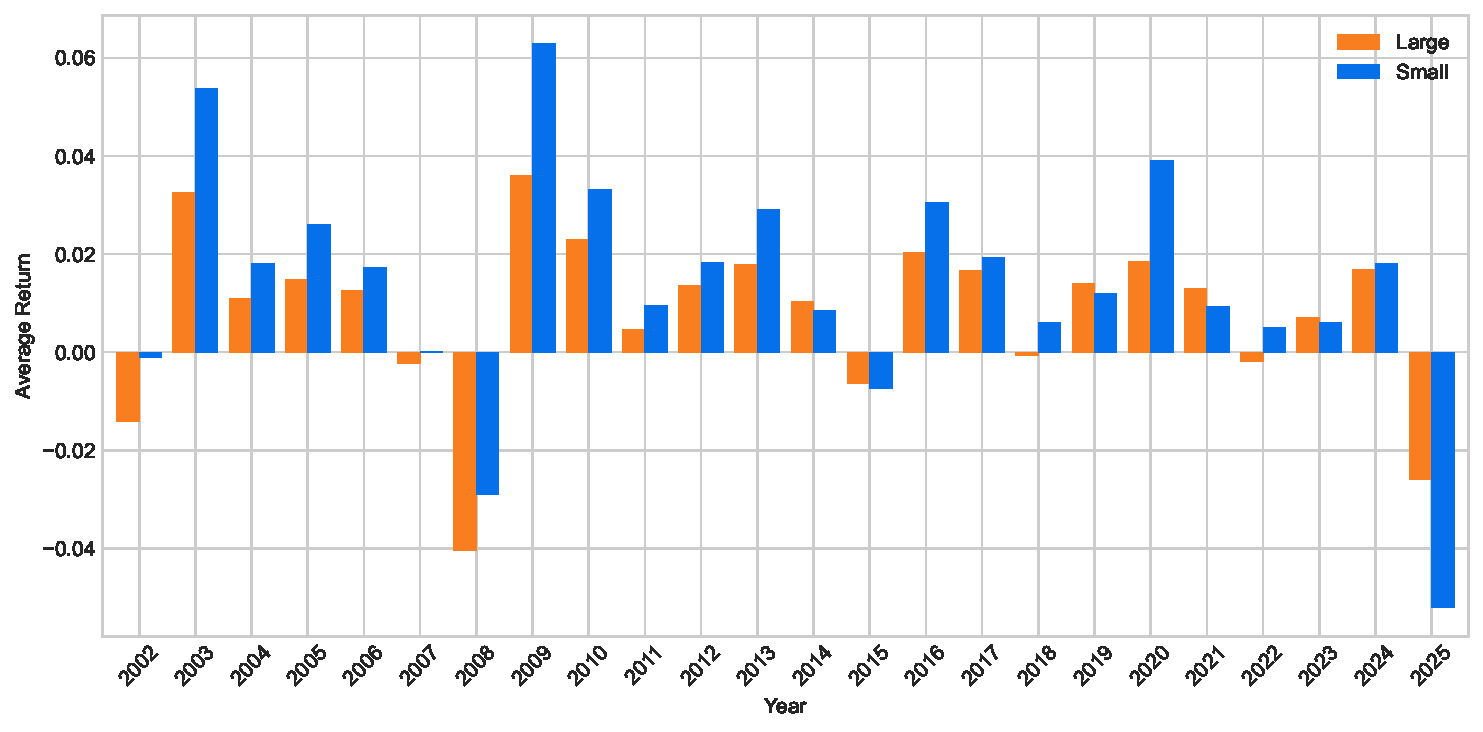
\includegraphics[width=0.7\linewidth]{files/48a05c076e107d524cdbc4ae811ead93.pdf}}
\label{fig-size_factor}
\end{figure}

\paragraph{Predictive regressions, sorts, and p-value issues}

For simplicity, we assume a simple form for stock returns (written in compact form):

\begin{equation}
\label{r}
\textbf{r} = a+b\textbf{x}+\textbf{e},
\end{equation}

where the vector $\textbf{r}$ stacks all returns of all stocks and $\textbf{x}$ is a lagged variable (e.g., a factor) so that the regression is indeed predictive. If the estimated $\hat{b}$ is significant given a specified confidence threshold, then it can be tempting to conclude that $\textbf{x}$ does a good job at predicting returns. Hence, long-short portfolios related to extreme values of $\textbf{x}$ (mind the sign of $\hat{b}$) are expected to generate profits. This is unfortunately often false because $\hat{b}$ gives information on the \textit{past} ability of $\textbf{x}$ to forecast returns. What happens in the future may be another story. In fact, as we discuss later, the problem is that it is mostly correlation that can be captured from financial data, whereas one would ideally prefer to infer \textit{causality} (see, e.g., \cite{de2026correcting}).

Statistical tests are also used for portfolio sorts. Assume two extreme portfolios are expected to yield very different average returns (like very small cap versus very large cap, or strong winners versus bad losers). The portfolio returns are written $r_t^+$ and $r_t^ -$. The simplest test for the mean is $t=\sqrt{T}\frac{m_{r_+} -m_{r_ -}}{\sigma_{r_+ -r_ -}}$, where $T$ is the number of points and $m_{r_\pm}$ denotes the means of returns and $\sigma_{r_+ -r_ -}$ is the standard deviation of the difference between the two series, i.e., the volatility of the long-short portfolio. In short, the statistic can be viewed as a scaled Sharpe ratio (though usually these ratios are computed for long-only portfolios) and can in turn be used to compute $p$-values to assess the robustness of an anomaly. As is shown in \cite{linnainmaa2018history} and \cite{hou2019replicating}, many factors discovered by reasearchers fail to survive in out-of-sample tests.

One reason why people are overly optimistic about anomalies they detect is the widespread reverse interpretation of the p-value. Often, it is thought of as the probability of one hypothesis (e.g., my anomaly exists) given the data. In fact, it's the opposite; it's the likelihood of your data sample, knowing that the anomaly holds.

\begin{align*}
p-\text{value} &= P[D|H] \\
\text{target prob.}& = P[H|D]=\frac{P[D|H]}{P[D]}\times P[H],
\end{align*}

where $H$ stands for hypothesis and $D$ for data. The equality in the second row is a plain application of Bayes' identity: the interesting probability is in fact a transform of the $p$-value.

Two articles (at least) discuss this idea. \cite{harvey2017presidential} introduces \textbf{Bayesianized} $p$-values:

\begin{equation}
\label{bayes_pvalue}
\text{Bayesianized } p-\text{value}=\text{Bpv}= e^{-t^2/2}\times\frac{\text{prior}}{1+e^{-t^2/2}\times \text{prior}},
\end{equation}

where $t$ is the $t$-statistic obtained from the regression (i.e., the one that defines the p-value) and prior is the analyst's estimation of the odds that the hypothesis (anomaly) is true. The prior is coded as follows. Suppose there is a p\% chance that the null holds (i.e., (1-p)\% for the anomaly). The odds are coded as $p/(1 -p)$. Thus, if the t-statistic is equal to 2 (corresponding to a p-value of 5\% roughly) and the prior odds are equal to 6, then the Bpv is equal to $e^{ -2}\times 6 \times(1+e^{ -2}\times 6)^{ -1}\approx 0.448$ and there is a 44.8\% chance that the null is true. This interpretation stands in sharp contrast with the original $p$-value which cannot be viewed as a probability that the null holds. Of course, one drawback is that the level of the prior is crucial and solely user-specified.

The work of \cite{chinco2019estimating} is very different but shares some key concepts, like the introduction of Bayesian priors in regression outputs. They show that coercing the predictive regression with an $L^2$ constraint (see the ridge regression in \href{/chap-06-lasso}{Chapter 5}) amounts to introducing views on what the true distribution of $b$ is. The stronger the constraint, the more the estimate $\hat{b}$ will be shrunk towards zero. One key idea in their work is the assumption of a distribution for the true $b$ across many anomalies. It is assumed to be Gaussian and centered. The interesting parameter is the standard deviation: the larger it is, the more frequently significant anomalies are discovered. Notably, the authors show that this parameter changes through time and we refer to the original paper for more details on this subject.

\paragraph{Fama-MacBeth regressions}

Another approach (one of the first in fact) was proposed by \cite{fama1973risk} through a two-stage regression analysis of risk premia. Take the average of Equation \ref{apt}:

\begin{equation}
\label{Er}
\mathbb{E}[\textbf{r}] = \alpha+\beta\mathbb{\textbf{f}},
\end{equation}

where the $\beta$ are the loadings and $\lambda = \mathbb{\textbf{x}}$ are the prices of risk, i.e., the risk premia. {\textbackslash}index\{risk premia\}
The first stage of the procedure is a simple estimation of the initial relationship: the regressions \ref{apt} are run on a stock-by-stock basis over the corresponding time series. The resulting estimates $\hat{\beta}_{i,k}$ are then plugged into a second series of regressions:

\begin{align*}
r_{t,n}= \gamma_{t,0} + \sum_{k=1}^K\gamma_{t,k}\hat{\beta}_{n,k} + \varepsilon_{t,n},
\end{align*}

which are run date-by-date on the cross-section of assets. Theoretically, the betas would be known and the regression would be run on the $\beta_{n,k}$ instead of their estimated values. The $\hat{\gamma}_{t,k}$ estimate the premia of factor $k$ at time $t$. Under suitable distributional assumptions on the $\varepsilon_{t,n}$, statistical tests can be performed to determine whether these premia are significant or not. Typically, the statistic on the time-aggregated (average) premia $\hat{\gamma}_k=\frac{1}{T}\sum_{t=1}^T\hat{\gamma}_{t,k}$:

\begin{align*}
t_k=\frac{\hat{\gamma}_k}{\hat{\sigma_k}/\sqrt{T}}
\end{align*}

is often used (under Gaussian assumptions) to assess whether or not the factor is significant ($\hat{\sigma}_k$ is the standard deviation of the $\hat{\gamma}_{t,k}$). In short:

\begin{itemize}
\item Step 1 (first pass) estimates what risks assets are exposed to;
\item Step 2 (second pass) estimates how the market prices those risks, period by period, and then averages.
\end{itemize}

We refer to \cite{jagannathan1998asymptotic} and \cite{petersen2009estimating} for technical discussions on the biases and losses in accuracy that can be induced by standard ordinary least squares (OLS) estimations. Moreover, as the $\hat\beta_{i,k}$ in the second-pass regression are estimates, a second level of errors can arise (the so-called errors in variables). The interested reader will find some extensions and solutions in \cite{shanken1992estimation}, \cite{ang2018using} and \cite{jegadeesh2019empirical}. There even exists a three-pass method (see \cite{giglio2018asset}).

A subtler issue concerns the \textit{strength} of the factors used in the first pass. \cite{pesaran2021factor} show that the standard two-pass estimator's properties depend critically on the degree of factor strength --- a continuous quantity, not the binary strong/weak dichotomy usually assumed. Empirically, among the five Fama-French factors, only the market factor can be classified as genuinely strong; the others are semi-strong at best, which affects the reliability of the estimated risk premia.

Below, we perform \cite{fama1973risk} regressions on our sample. We first build a dedicated dataset.

\begin{verbatim}
# Select a subset of stocks for the Fama-MacBeth analysis
stock_ids_short = data_ml['fsym_id'].unique()[:30]

# Prepare data: merge returns with factors
returns_subset = data_ml[data_ml['fsym_id'].isin(stock_ids_short)][['date', 'fsym_id', 'R1M']]
returns_pivot = returns_subset.pivot(index='date', columns='fsym_id', values='R1M')

# Merge with factors
data_FM = returns_pivot.join(FF_factors.set_index('date')[['MKT_RF', 'SMB', 'HML', 'RMW', 'CMA']])

# Select a subset of stocks for the Fama-MacBeth analysis
stock_ids_short = data_ml['fsym_id'].unique()[:30]

# Prepare data: merge returns with factors
returns_subset = data_ml[data_ml['fsym_id'].isin(stock_ids_short)][['date', 'fsym_id', 'R1M']]
returns_pivot = returns_subset.pivot(index='date', columns='fsym_id', values='R1M')

# Merge with factors
data_FM = returns_pivot.join(FF_factors.set_index('date')[['MKT_RF', 'SMB', 'HML', 'RMW', 'CMA']])
data_FM = data_FM.dropna()

print(f"Data shape for FM regressions: {data_FM.shape}")
\end{verbatim}

\begin{verbatim}
Data shape for FM regressions: (36, 35)
\end{verbatim}

Then we move onto the first pass: individual estimation of betas. To do so, we loop across stocks and provide a snapshot of estimates.

\begin{figure}
\centering
\begin{verbatim}
# First pass: estimate betas for each stock
factor_cols = ['MKT_RF', 'SMB', 'HML', 'RMW', 'CMA']
betas = {}
for fsym_id in stock_ids_short:
    if fsym_id in data_FM.columns:
        y = data_FM[fsym_id].shift(-1).dropna()  # Lagged returns
        X = data_FM[factor_cols].loc[y.index]
        X = sm.add_constant(X)
        # Drop any remaining NaN
        mask = ~(y.isna() | X.isna().any(axis=1))
        y_clean = y[mask]
        X_clean = X[mask]
        if len(y_clean) > 10:  # Minimum number of observations
            model = sm.OLS(y_clean, X_clean).fit()
            betas[fsym_id] = model.params
# Convert to DataFrame & show
betas_df = pd.DataFrame(betas).T
betas_df.columns = ['Constant'] + factor_cols
betas_df.head(6).round(3)
\end{verbatim}
\caption[]{Sample of beta values.

\begin{tabular}{p{\dimexpr 0.143\linewidth-2\tabcolsep}p{\dimexpr 0.143\linewidth-2\tabcolsep}p{\dimexpr 0.143\linewidth-2\tabcolsep}p{\dimexpr 0.143\linewidth-2\tabcolsep}p{\dimexpr 0.143\linewidth-2\tabcolsep}p{\dimexpr 0.143\linewidth-2\tabcolsep}p{\dimexpr 0.143\linewidth-2\tabcolsep}}
\toprule
 & Constant & MKT\_RF & SMB & HML & RMW & CMA \\
\hline
1105 & -0.013 & 1.004 & 1.011 & -2.289 & 2.425 & -0.201 \\
\hline
2072 & 0.076 & 0.459 & -0.625 & -3.475 & -6.032 & 2.155 \\
\hline
2859 & 0.025 & 0.270 & -0.284 & -1.492 & -1.586 & 0.176 \\
\hline
1627 & 0.041 & 0.378 & -1.375 & -0.586 & 0.829 & 1.202 \\
\hline
2524 & 0.010 & 1.817 & -2.627 & -2.521 & -3.071 & 1.801 \\
\hline
2611 & 0.008 & 0.210 & 0.014 & -0.094 & 0.682 & 0.777 \\
\hline
\bottomrule
\end{tabular}}
\label{tab-sample-betas}
\end{figure}

In the table, MKT\_RF is the market return minus the risk free rate. The corresponding coefficient is often referred to as the beta, especially in univariate regressions. We then reformat these betas from the table to prepare the second pass. Each line corresponds to one asset: the first 5 columns are the estimated factor loadings and the remaining ones are the asset returns (date by date).

\begin{figure}
\centering
\begin{verbatim}
# Second pass: cross-sectional regressions
loadings = betas_df[factor_cols]
returns_for_FM = returns_pivot[loadings.index].T  # Transpose: stocks as rows, dates as columns

# Run cross-sectional regressions for each date
gammas = {}
for date in returns_for_FM.columns:
    y = returns_for_FM[date].dropna()
    X = loadings.loc[y.index]
    X = sm.add_constant(X)
    if len(y) > 5:  # Minimum observations
        model = sm.OLS(y, X).fit()
        gammas[date] = model.params

# Convert to DataFrame
gammas_df = pd.DataFrame(gammas).T
gammas_df.columns = ['Constant'] + factor_cols
gammas_df.head(6).round(3)
\end{verbatim}
\caption[]{Sample of gamma (premia) values.

\begin{tabular}{p{\dimexpr 0.143\linewidth-2\tabcolsep}p{\dimexpr 0.143\linewidth-2\tabcolsep}p{\dimexpr 0.143\linewidth-2\tabcolsep}p{\dimexpr 0.143\linewidth-2\tabcolsep}p{\dimexpr 0.143\linewidth-2\tabcolsep}p{\dimexpr 0.143\linewidth-2\tabcolsep}p{\dimexpr 0.143\linewidth-2\tabcolsep}}
\toprule
 & Constant & MKT\_RF & SMB & HML & RMW & CMA \\
\hline
2007-07-31 & -0.466 & -1.203 & 0.623 & -0.348 & 0.174 & 0.611 \\
\hline
2007-08-31 & -0.090 & -0.056 & 0.034 & -0.177 & 0.063 & 0.057 \\
\hline
2007-09-30 & 0.087 & -0.100 & -0.088 & -0.049 & 0.009 & 0.013 \\
\hline
2007-10-31 & -0.027 & -0.223 & -0.081 & -0.054 & 0.055 & -0.029 \\
\hline
2007-11-30 & -0.041 & -0.201 & -0.070 & -0.045 & -0.025 & -0.014 \\
\hline
2007-12-31 & -0.072 & 0.061 & -0.014 & 0.062 & -0.007 & -0.001 \\
\hline
\bottomrule
\end{tabular}}
\label{tab-sample-gammas}
\end{figure}

Visually, the estimated premia are also very volatile. We plot in Figure~\ref{fig-ts-gammas} their estimated values for the market, SMB and HML factors.

\begin{figure}[!htbp]
\centering
\begin{verbatim}
# Plot time series of gammas (premia)
fig, axes = plt.subplots(3, 1, figsize=(12, 8), sharex=True)

factors_plot = ['MKT_RF', 'SMB', 'HML']
colors = ['#F87E1F', '#0570EA', '#F81F40']

for ax, factor, color in zip(axes, factors_plot, colors):
    ax.plot(gammas_df.index, gammas_df[factor], color=color, linewidth=0.8)
    ax.set_ylabel(factor)
    ax.axhline(y=0, color='gray', linestyle='--', alpha=0.5)

axes[-1].set_xlabel('Date')
fig.suptitle('Time Series of Gammas (Premia) in Fama-MacBeth Regressions', y=1.02)
plt.tight_layout()
plt.show()
\end{verbatim}
\caption[]{Time-series of gamma values (premia).

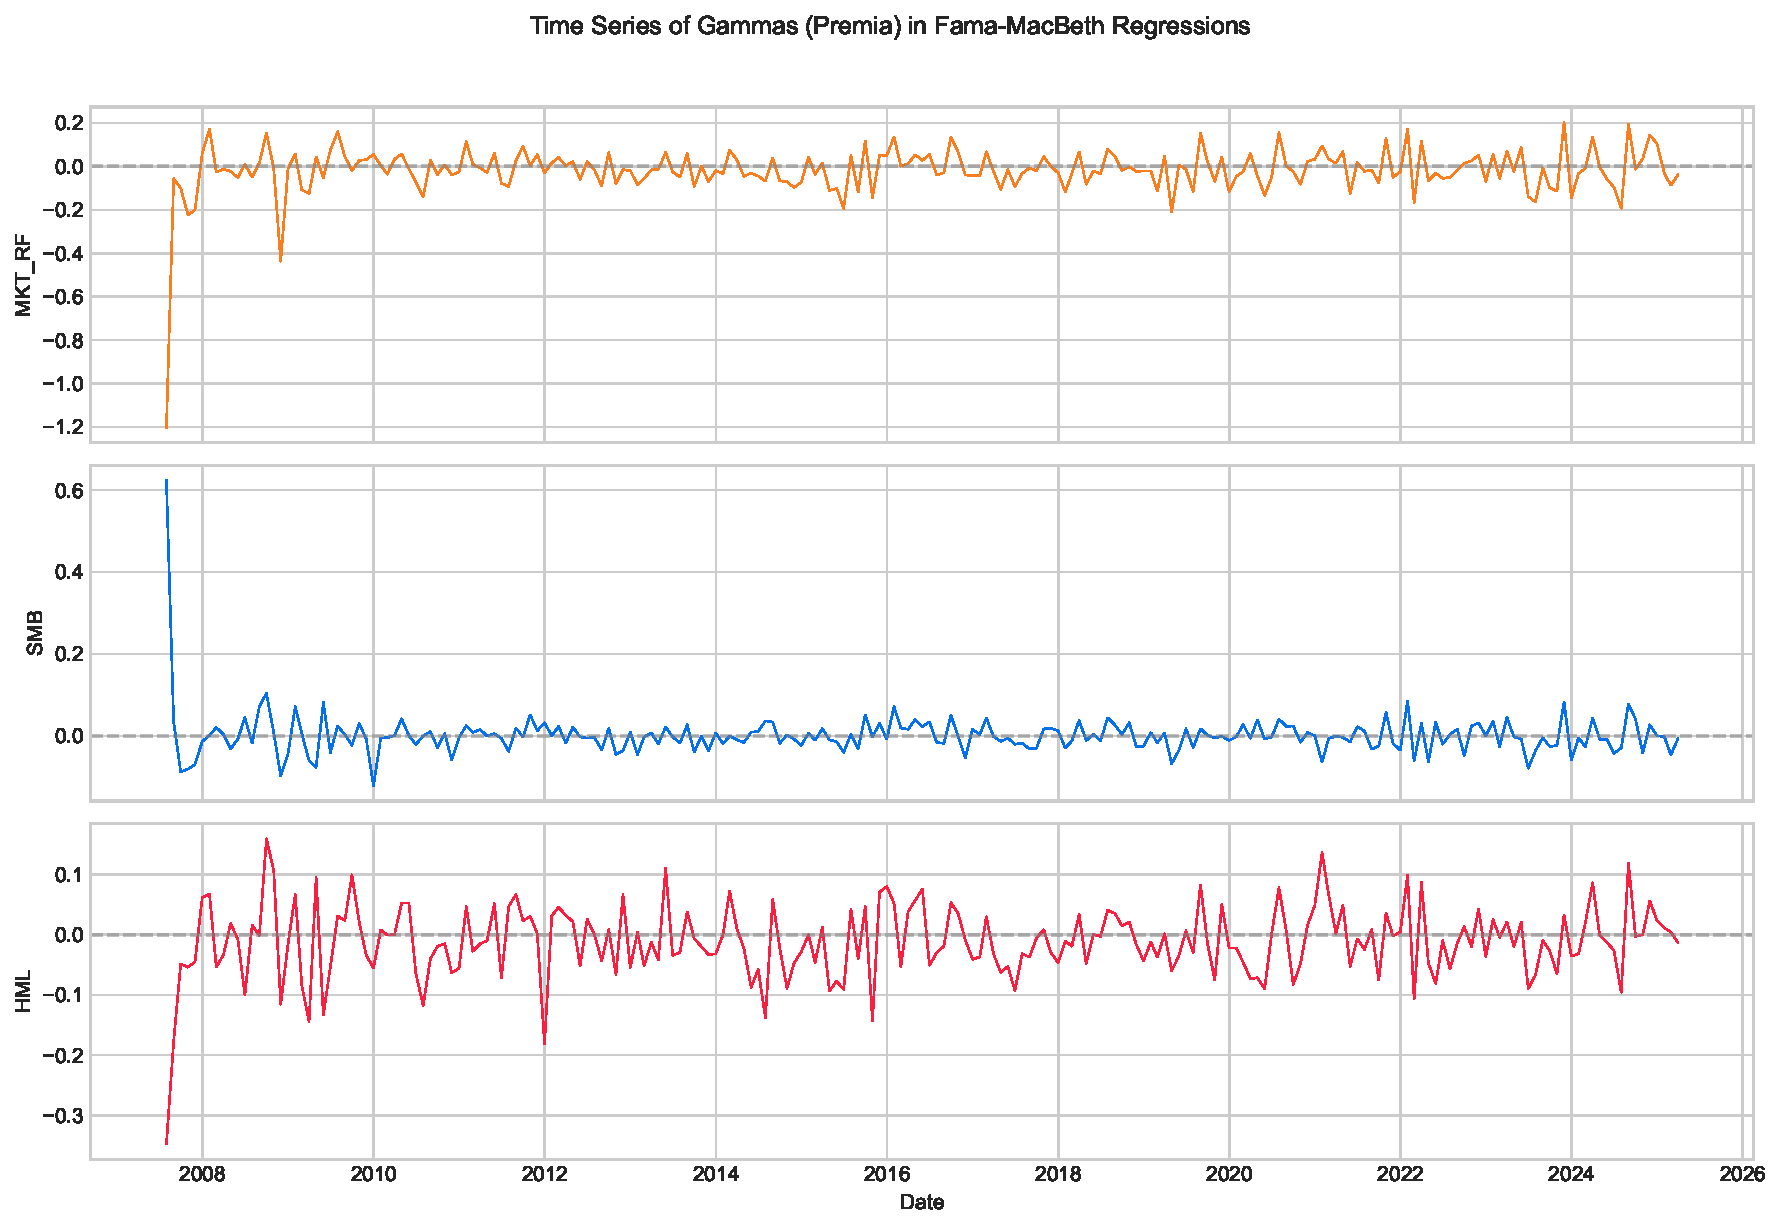
\includegraphics[width=0.7\linewidth]{files/46605f13fe30014eb492dc3ba50c9266.pdf}}
\label{fig-ts-gammas}
\end{figure}

\paragraph{Factor competition and redundancy}

The core purpose of factors is to explain the cross-section of stock returns. For theoretical and practical reasons, it is preferable to avoid redundancies within factors. Indeed, redundancies imply collinearity which is known to perturb estimates \citep{belsley2005regression}. In addition, when asset managers decompose the performance of their returns into factors, overlaps (high absolute correlations) between factors yield exposures that are less interpretable; positive and negative exposures compensate each other spuriously.

A simple protocol to sort out redundant factors is to run regressions of each factor against all others:

\begin{equation}
\label{f_competition}
f_{t,k} = a_k +\sum_{j\neq k} \delta_{k,j} f_{t,j} + \epsilon_{t,k}.
\end{equation}

The interesting metric is then the test statistic associated to the estimation of $a_k$. If $a_k$ is significantly different from zero (i.e., the statistic has magnitude larger than 2 or 3), then the cross-section of (other) factors fails to explain exhaustively the average return of factor $k$. Otherwise, the return of the factor can be captured by exposures to the other factors and is thus redundant.

One mainstream application of this technique was performed in \cite{fama2015five}, in which the authors show that the HML factor is redundant when taking into account four other factors (Market, SMB, RMW and CMA). Below, we reproduce their analysis on an updated sample. We start our analysis directly with the database maintained by Kenneth French.

We can run the regressions that determine the redundancy of factors via the procedure defined in Equation \ref{f_competition}.

\begin{verbatim}
# Factor competition analysis
factors = ['MKT_RF', 'SMB', 'HML', 'RMW', 'CMA']
results = []
for dep_var in factors:
    other_factors = [f for f in factors if f != dep_var]
    y = FF_factors[dep_var]
    X = FF_factors[other_factors]
    X = sm.add_constant(X)
    model = sm.OLS(y, X).fit()
    row = {'Dep. Variable': dep_var}
    coef = model.params['const']
    pval = model.pvalues['const']
    row['Intercept'] = f"{coef:.3f}" + get_significance(pval)
    for factor in factors:
        if factor == dep_var:
            row[factor] = '-'
        else:
            coef = model.params[factor]
            pval = model.pvalues[factor]
            row[factor] = f"{coef:.3f}" + get_significance(pval)
    results.append(row)
\end{verbatim}

We obtain the vector of $\alpha$ values from Equation \ref{f_competition}. Below, we format these figures along with $p$-value thresholds and export them in a summary table (Figure~\ref{fig-factor_competition}). The significance levels of coefficients is coded as follows: $0<(***)<0.001<(**)<0.01<(*)<0.05$

\begin{verbatim}
factor_competition_df = pd.DataFrame(results)
print("Significance: *** p<0.001, ** p<0.01, * p<0.05")
\end{verbatim}

\begin{verbatim}
Significance: *** p<0.001, ** p<0.01, * p<0.05
\end{verbatim}

\begin{figure}
\centering
\begin{verbatim}
factor_competition_df
\end{verbatim}
\caption[]{Factor Competition among the five Fama-French Factors.

\begin{tabular}{p{\dimexpr 0.125\linewidth-2\tabcolsep}p{\dimexpr 0.125\linewidth-2\tabcolsep}p{\dimexpr 0.125\linewidth-2\tabcolsep}p{\dimexpr 0.125\linewidth-2\tabcolsep}p{\dimexpr 0.125\linewidth-2\tabcolsep}p{\dimexpr 0.125\linewidth-2\tabcolsep}p{\dimexpr 0.125\linewidth-2\tabcolsep}p{\dimexpr 0.125\linewidth-2\tabcolsep}}
\toprule
 & Dep. Variable & Intercept & MKT\_RF & SMB & HML & RMW & CMA \\
\hline
0 & MKT\_RF & 0.008 (***) & - & 0.292 (***) & 0.115 & -0.257 (***) & -0.856 (***) \\
\hline
1 & SMB & 0.002 (*) & 0.136 (***) & - & 0.157 (**) & -0.445 (***) & -0.184 (*) \\
\hline
2 & HML & -0.001 & 0.032 & 0.094 (**) & - & 0.179 (***) & 1.030 (***) \\
\hline
3 & RMW & 0.004 (***) & -0.066 (***) & -0.247 (***) & 0.166 (***) & - & -0.257 (***) \\
\hline
4 & CMA & 0.002 (***) & -0.105 (***) & -0.048 (*) & 0.453 (***) & -0.122 (***) & - \\
\hline
\bottomrule
\end{tabular}}
\label{fig-factor_competition}
\end{figure}

We confirm that the HML factor remains redundant when the four others are present in the asset pricing model (its alpha - in the Intercept column - is not significantly different from zero). The figures we obtain are reasonably close to the ones in the original paper \citep{fama2015five}, which makes sense, since we ``only'' add 15 years to their initial sample.

At a more macro-level, researchers also try to figure out which models (i.e., combinations of factors) are the most likely, given the data empirically observed (and possibly given priors formulated by the econometrician). For instance, this stream of literature seeks to quantify to which extent the 3-factor model of \cite{fama1993common} outperforms the 5 factors in \cite{fama2015five}. In this direction, \cite{de2015comparing} introduce a novel computation for p-values that compare the relative likelihood that two models pass a zero-alpha test. More generally, the Bayesian method of \cite{barillas2018comparing} was subsequently improved by \cite{chib2021winners}.

Lastly, even the optimal \textbf{number of factors} is a subject of disagreement among conclusions of recent work. While the traditional literature focuses on a limited number (3-5) of factors, more recent research by \cite{martin2018transaction}, \cite{he2019factors}, \cite{kozak2019shrinking} and \cite{freyberger2020dissecting} advocates the need to use at least 15 or more. \cite{kozak2019shrinking} provide perhaps the strongest counter-evidence, arguing that ``\textit{the quest for a sparse characteristics-based factor model is ultimately futile}'' since such models fail out-of-sample. A middle ground emerges from \cite{kelly2019characteristics}, who find that only 10 characteristics (or \textbf{latent} factors) are significant in their IPCA framework, and \cite{swade2024factor}, who conclude that approximately 15 factors span the zoo---more than traditional models but far fewer than hundreds. The synthesis suggests that while extreme factor proliferation reflects data mining (see \cite{chen2024does}), traditional 3--6 factor models likely underfit the true complexity; dimension reduction to 10--15 factors or latent components offers the best balance between overfitting and explanatory power. \cite{green2017characteristics} even find that the number of characteristics that help explain the cross-section of returns varies in time.

Complementing these cross-sectional approaches, \cite{odoherty2025macroeconomic} take a different angle by estimating risk premia for 190 candidate macroeconomic factors. They find that more than 40 carry significant premia, and that parsimonious two-factor models pairing the market with a single macro factor (especially those tied to national income accounts or housing) frequently outperform leading multifactor models in explaining CAPM anomalies. This suggests that the factor zoo may partly reflect a disconnect between financial and macroeconomic research traditions.

\cite{huang2026identity} introduce the concept of \textit{factor identities}, groups of factors that carry identical pricing information for the cross section of expected returns despite modest time series correlations. Using a Bayesian approach, they show that the factor zoo is dense in individual variables but sparse in underlying economic species. The stochastic discount factor is driven mainly by three identities: a macroeconomic identity captured by long horizon GDP growth, a market identity reflecting aggregate risk premia, and a latent statistical identity that subsumes most characteristic based factors.

\paragraph{Advanced selection techniques}

The ever increasing number of factors combined to their importance in asset management has led researchers to craft more subtle methods in order to ``organize'' the so-called \textit{factor zoo} {\textbackslash}index\{factor zoo\} and, more importantly, to detect spurious anomalies and compare different asset pricing model specifications. We list a few of them below.

\begin{itemize}
\item \cite{feng2019taming} combine LASSO selection with Fama-MacBeth regressions to test if new factor models are worth it. They quantify the gain of adding one new factor to a set of predefined factors and show that many factors reported in papers published in the 2010 decade do not add much incremental value;
\item \cite{harvey2017lucky}, in a similar vein, use bootstrap on orthogonalized factors. They make the case that correlations among predictors is a major issue and their method aims at solving this problem. Their lengthy procedure seeks to test if maximal additional contribution of a candidate variable is significant;
\item \cite{fama2018choosing} compare asset pricing models through squared maximum Sharpe ratios;
\item \cite{giglio2018asset} estimate factor risk premia using a three-pass method based on principal component analysis;
\item \cite{pukthuanthong2018protocol} disentangle priced and non-priced factors via a combination of principal component analysis and \cite{fama1973risk} regressions;
\item \cite{gospodinov2019too} warn against factor misspecification (when spurious factors are included in the list of regressors). Traded factors (\textit{resp}., macro-economic factors) seem more likely (\textit{resp}., less likely) to yield robust identifications (see also \cite{bryzgalova2019spurious});
\item \cite{harvey2026threshold} revisit the multiple hypothesis testing problem in factor model evaluation and reconcile contradictory findings about the replication crisis. Proper inference requires accounting for dependence across tests, correctly specifying the null distribution, and mitigating sample-selection bias; the authors advocate a $t$-statistic cutoff of at least 3.0 and the use of local False Discovery Rates;
\item \cite{danagel2024statistical} investigate the statistical limits of arbitrage in high dimensions. When alphas are weak and rare, estimation errors prevent even optimally-equipped ML arbitrageurs from fully exploiting pricing errors, creating a significant gap between the feasible and theoretical maximum Sharpe ratios. This result provides a theoretical ceiling on what ML-based strategies can achieve.
\item \cite{davis2026complexity} show theoretically that APT pricing errors do not vanish as markets grow but instead scale linearly with the number of assets. Because estimation errors are multidimensional and do not diversify away like idiosyncratic risk, the stochastic discount factor loads primarily on those errors rather than on fundamental risk. One implication is that a proliferation of weakly correlated, high Sharpe strategies can coexist in equilibrium as investors exploit distinct dimensions of growing estimation uncertainty.
\end{itemize}

There is obviously no infallible method, but the number of contributions in the field highlights the need for robustness. This is evidently a major concern when crafting investment decisions based on factor intuitions. One major hurdle for short-term strategies is the likely time-varying feature of factors. We refer for instance to \cite{ang2012testing} and \cite{cooper2018new} for practical results and to \cite{gagliardini2016time} and S. \cite{ma2018testing} for more theoretical treatments (with additional empirical results).

\subsubsection{Factors or characteristics?}

The decomposition of returns into linear factor models is convenient because of its simple interpretation. There is nonetheless a debate in the academic literature about whether firm returns are indeed explained by exposure to macro-economic factors or simply by the characteristics of firms. In their early study, \cite{lakonishok1994contrarian} argue that one explanation of the value premium comes from incorrect extrapolation of past earning growth rates. Investors are overly optimistic about firms subject to recent profitability. Consequently, future returns are (also) driven by the core (accounting) features of the firms. The question is then to disentangle which effect is the most pronounced when explaining returns: characteristics versus exposures to macro-economic factors.

In their seminal contribution on this topic, \cite{daniel1997evidence} provide evidence in favour of the former (two follow-up papers are K. \cite{daniel2001overconfidence} and \cite{daniel2012testing}). They show that firms with high book-to-market ratios or small capitalizations display higher average returns, even if they are negatively loaded on the HML or SMB factors. Therefore, it seems that it is indeed the \textbf{intrinsic characteristics} that matter, and not the factor exposure. For further material on characteristics' role in return explanation or prediction, we refer to the following contributions:

\begin{itemize}
\item Section 2.5.2. in \cite{goyal2012empirical} surveys pre-2010 results on this topic;
\item \cite{chordia2015cross} find that characteristics explain a larger proportion of variation in estimated expected returns than factor loadings;
\item \cite{kozak2018interpreting} reconcile factor-based explanations of premia to a theoretical model in which some agents' demands are sentiment driven;
\item \cite{han2018firm} show with penalized regressions that 20 to 30 characteristics (out of 94) are useful for the prediction of monthly returns of US stocks. Their methodology is interesting: they regress returns against characteristics to build forecasts and then regress the returns on the forecast to assess if they are reliable. The latter regression uses a LASSO-type penalization (see Chapter 5) so that useless characteristics are excluded from the model. The penalization is extended to elasticnet in \cite{rapach2019time}.
\item \cite{kelly2019characteristics} and \cite{kim2019arbitrage} both estimate models in which factors are latent but loadings (betas) and possibly alphas depend on characteristics. \cite{kirby2020firm} generalizes the first approach by introducing regime-switching. In contrast, \cite{lettau2018estimating} and \cite{lettau2018estimating} estimate latent factors without any link to particular characteristics (and provide large sample asymptotic properties of their methods).
\item In the same vein as \cite{hoechle2018correcting}, \cite{gospodinov2019too} and \cite{bryzgalova2019spurious} and discuss potential errors that arise when working with portfolio sorts that yield long-short returns. The authors show that in some cases, tests based on this procedure may be deceitful. This happens when the characteristic chosen to perform the sort is correlated with an external (unobservable) factor. They propose a novel regression-based approach aimed at bypassing this problem.
\item Even \cite{fama2020comparing} conclude: ``\textit{time-series models that use only cross-section factors provide better descriptions of average returns than time-series models that use time-series factors}''.
\end{itemize}

More recently and in a separate stream of literature, \cite{koijen2019investors} have introduced a demand model in which investors form their portfolios according to their preferences towards particular firm characteristics. They show that this allows them to mimic the portfolios of large institutional investors. In their model, aggregate demands (and hence, prices) are directly linked to characteristics, not to factors. In a follow-up paper, \cite{koijen2019investors} show that a few sets of characteristics suffice to predict future returns. They also show that, based on institutional holdings from the UK and the US, the largest investors are those who are the most influencial in the formation of prices. In a similar vein, \cite{betermier2019supply} derive an elegant (theoretical) general equilibrium model that generates some well-documented anomalies (size, book-to-market). The models of \cite{arnott2014can} and \cite{alti2019dynamic} are also able to theoretically generate known anomalies. Finally, in \cite{martin2019bayesian}, characteristics influence returns via the role they play in the predictability of dividend growth. This paper discussed the asymptotic case when the number of assets and the number of characteristics are proportional and both increase to infinity.

Several recent contributions push the characteristics-based view further. \cite{ge2021dynamic} propose a semi-parametric model with B-spline sieves and use hierarchical clustering to identify ``peer groups'' of characteristics that lead to similar arbitrage returns, revealing structure in the mispricing component. In a different vein, \cite{cartea2025learning} introduce a self-supervised tabular transformer that compresses over 400 firm characteristics into low-dimensional embeddings capturing both cross-sectional and temporal patterns. These embeddings yield similarity-based strategies that outperform standard benchmarks, suggesting that the relevant information in characteristics may be better captured by learned representations than by hand-picked subsets. \cite{gabaix2025asset} take a related approach using transformer architectures trained on institutional portfolio holdings. Asset embeddings derived from this procedure explain over 50\% of the variation in relative valuations, compared with around 15\% for traditional firm characteristics. Economic content is recovered by linking the embeddings to earnings calls and prospectus text via large language models.

\subsubsection{Demand-based asset pricing}

As introduced at the beginning of this chapter, the demand-system approach of \cite{koijen2019demand} provides a theoretical foundation linking firm characteristics to equilibrium prices through portfolio demand. This framework has generated substantial follow-up work that we review here.

\textbf{Theoretical foundations.} \cite{fuchs2025demand} show that the original framework does not adequately account for cross-asset complementarities in portfolio choice, leading to significantly biased demand elasticity estimates. Measured elasticities can appear close to one even when the true values are near-infinite, which helps reconcile the striking gap between low demand-system estimates and higher theoretical benchmarks from other approaches.

\textbf{Identification challenges.} \cite{vanbinsbergen2025identification} establish strict necessary conditions for valid identification of demand elasticities in dynamic markets. Instruments borrowed from static industrial organization models introduce large biases when applied to financial assets. Valid instruments must induce price variation lasting at most one trading period and be unanticipated ex ante --- a demanding requirement that calls into question many existing empirical estimates.

\textbf{Extensions.} \cite{gehrig2024extending} generalize the framework beyond log-utility to constant absolute and constant relative risk aversion preferences. They also introduce a shrinkage device that pulls portfolio weights toward a predetermined policy portfolio, reducing parameter uncertainty and outperforming both the parametric approach and naive $1/N$ strategies empirically.

These developments show that while the demand-system approach offers a compelling structural link between characteristics and prices, its empirical implementation remains delicate. The interplay between investor heterogeneity, preference specification, and identification strategy is an active and rapidly evolving research frontier.

\subsubsection{Factor dynamics: momentum, timing, and ESG}

\paragraph{Factor momentum}

A recent body of literature unveils a time series momentum property of factor returns. For instance, \cite{gupta2019factor} report that autocorrelation patterns within these returns is statistically significant. Autocorrelation in aggregate/portfolio returns is a widely documented effect since the seminal paper \cite{lo1990contrarian} (see also \cite{moskowitz2012time}). Similar results are obtained in \cite{falck2020factor}. In the same vein, \cite{arnott2019factor} make the case that the industry momentum found in \cite{moskowitz1999industries} can in fact be explained by this factor momentum. Going even further, \cite{ehsani2019factor} conclude that the original momentum factor is in fact the aggregation of the autocorrelation that can be found in all other factors. Recently, the strength of factor momentum is scrutinized by \cite{fan2021reexamination}. The authors find that it is only robust for a small number of factors. Lastly, \cite{garcia2021factor} document factor momentum at the daily frequency.

Acknowledging the profitability of factor momentum, \cite{yang2020decomposing} seeks to understand its source and decomposes stock factor momentum portfolios into two components: factor timing portfolio and a static portfolio. The former seeks to profit from the serial correlations of factor returns while the latter tries to harness factor premia. The author shows that it is the static portfolio that explains the larger portion of factor momentum returns. In \cite{yang2020weighted}, the same author presents a new estimator to gauge factor momentum predictability. Words of caution are provided in \cite{leippold2021anatomy}.

Given the data obtained on \href{https://mba.tuck.dartmouth.edu/pages/faculty/ken.french/data\_library.html}{Ken French's website}, we compute the autocorrelation function (ACF) of factors.

\begin{equation}
\label{acf}
\text{ACF}_k(\textbf{x}_t)=\mathbb{E}[(\textbf{x}_t-\bar{\textbf{x}})(\textbf{x}_{t+k}-\bar{\textbf{x}})].
\end{equation}

\begin{verbatim}
# ACF plots for factor returns
fig, axes = plt.subplots(2, 2, figsize=(12, 8))

factors_acf = ['SMB', 'HML', 'RMW', 'CMA']

for ax, factor in zip(axes.flatten(), factors_acf):
    plot_acf(FF_factors[factor].dropna(), ax=ax, zero=False, lags=10, title=f'ACF - {factor}')
    ax.set_ylim(-0.08, 0.2)

plt.tight_layout()
plt.show()
\end{verbatim}

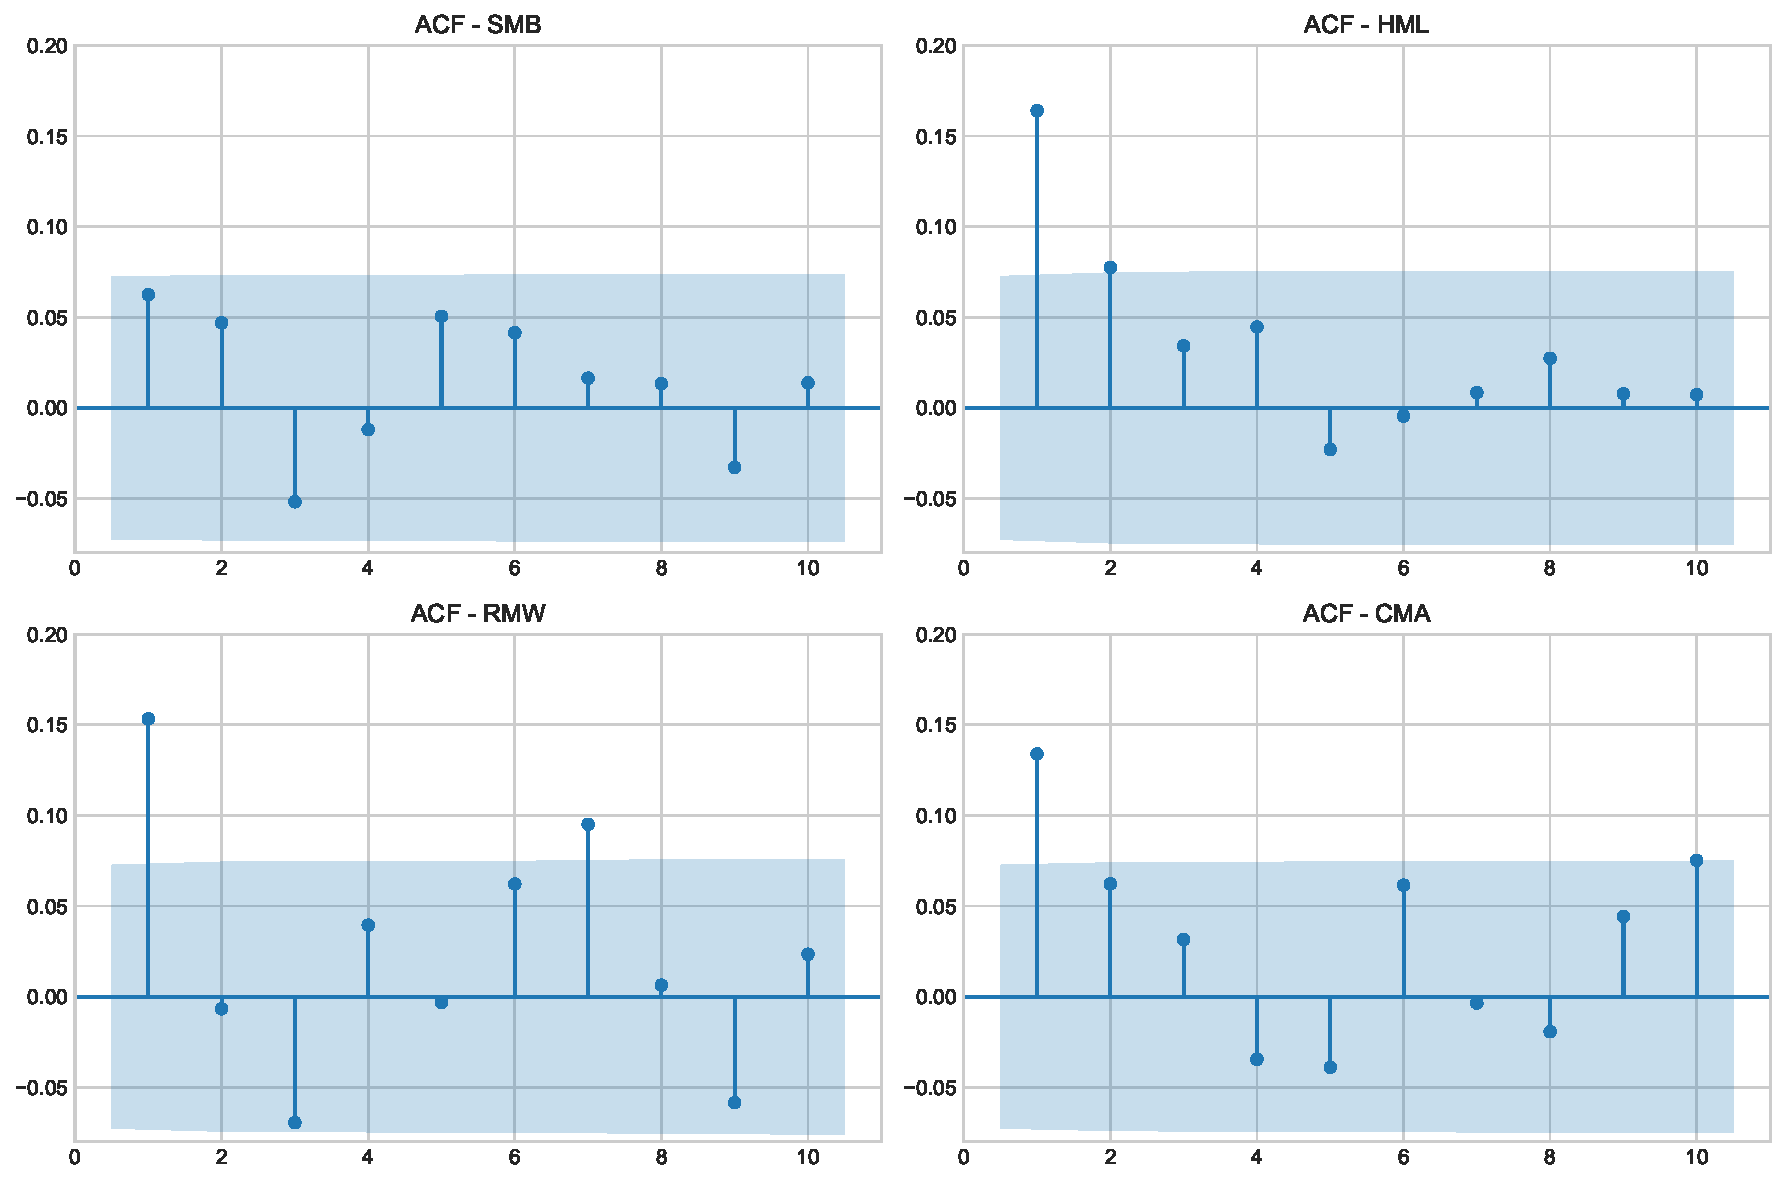
\includegraphics[width=0.7\linewidth]{files/e28136d561ef2a39181beb04a2e9f6bd.pdf}

FIGURE 3.4: Autocorrelograms of common factor portfolios.

Of the four chosen series, only the size factor is not significantly autocorrelated at the first order.

\paragraph{Factor timing}

Given the abundance of evidence of the time-varying nature of factor premia, it is legitimate to wonder if it is possible to predict when factor will perform well or badly. The evidence on the effectiveness of timing is diverse:

\begin{itemize}
\item \textbf{positive} for \cite{greenwood2012share}, \cite{hodges2017factor}, \cite{hasler2019should}, \cite{haddad2020economics}, \cite{lioui2020factor}, \cite{neuhierl2023timing} and \cite{lehnherr2024optimal};
\item \textbf{negative} for \cite{asness2017contrarian}; and
\item \textbf{mixed} for \cite{dichtl2019optimal}.
\end{itemize}

We nevertheless underline that the dominant share of favorable findings may be due to the publishing bias towards positive results. There is no consensus on which predictors to use (general macroeconomic indicators in \cite{hodges2017factor}, stock issuances versus repurchases in \cite{greenwood2012share}, and aggregate fundamental data in \cite{dichtl2019optimal}). In fact, it might be best to consider many variables \citep{kagkadis2021factor}.

A method for building reasonable timing strategies for long-only portfolios with sustainable transaction costs is laid out in \cite{leippold2020fama}. In ML-based factor investing, it is possible to resort to more granularity by combining firm-specific attributes to macro-economic data as we explain in Section~\ref{sec_macrovar}.

On the question of whether \textit{any} strategy --- traditional or ML-based --- can reliably time factors, \cite{allen2026adaptive} provide a comprehensive evaluation over 1970--2024. They find that no strategy delivers robust unconditional alpha relative to buy-and-hold, consistent with market efficiency. However, conditioning on an ``ecology vector'' capturing crowding, funding, liquidity, and volatility reveals systematic state-dependent performance variation, supporting the Adaptive Markets Hypothesis of \cite{lo2004adaptive}. This suggests that factor timing may work, but only intermittently and for agents who can identify the right market regime.

\paragraph{The green factors}

The demand for ethical financial products has sharply risen during the 2010 decade, leading to the creation of numerous funds dedicated to socially responsible investing (SRI - see \cite{camilleri2020market}). Though this phenomenon is not really new (\cite{schueth2003socially}, \cite{hill2007corporate}), its acceleration has prompted research about whether or not characteristics related to ESG criteria (environment, social, governance) are priced.

Dozens and even possibly hundreds of papers have been devoted to this question, but no consensus has been reached. More and more, researchers study the financial impact of climate change (see \cite{bernstein2019disaster}, \cite{hong2019climate} and \cite{hong2020climate}) and the societal push for responsible corporate behavior (\cite{fabozzi2020introduction}, \cite{kurtz2020three}). We gather below a very short list of early papers that suggests conflicting results (see \cite{coqueret2022perspectives} for a more detailed account):

\begin{itemize}
\item \textbf{favorable}: ESG investing works (\cite{kempf2007effect}, \cite{cheema2020decarbonization}), can work (\cite{nagy2016can}, \cite{alessandrini2020optimal}), or can at least be rendered efficient \citep{branch2012socially}. A large meta-study reports overwhelming favorable results \citep{friede2015esg}, but of course, they could well stem from the publication bias towards positive results.
\item \textbf{unfavorable}: Ethical investing is not profitable according to \cite{adler2008cost} and \cite{blitz2020exclusion}. An ESG factor should be long unethical firms and short ethical ones \citep{lioui2018esg}.
\item \textbf{mixed}: ESG investing may be beneficial globally but not locally \citep{chakrabarti2020time}. Portfolios relying on ESG screening do not significantly outperform those with no screening but are subject to lower levels of volatility (\cite{gibson2020responsible}, \cite{gougler2020factor}). As is often the case, the devil is in the details, and results depend on whether to use E, S or G \citep{bruder2019integration}.
\end{itemize}

On top of these contradicting results, several articles point towards complexities in the measurement of ESG. Depending on the chosen criteria and on the data provider, results can change drastically, a phenomenon known as \textbf{ESG confusion} or \textbf{ESG divergence} (see \cite{galema2008stocks}, \cite{atta2020strategies}, \cite{dimson2020divergent}, \cite{avramov2022sustainable} and \cite{berg2019aggregate}). Two large-scale studies (\cite{beyer2024non} and \cite{alves2025drawing}) show that the performance of ESG-related portfolios also varies across time, geographies, sectors, etc. But overall, it is hard to conclude that sustainability is priced. We end this short section by noting that, of course, ESG criteria can directly be integrated into ML model, as is for instance done in \cite{de2020esg}, and they can also be complemented by traditional firm characteristics \citep{coqueret2022enhancing}.

\subsubsection{Machine learning meets asset pricing}

\paragraph{The canonical predictive model}

Given the exponential increase in data availability, the obvious temptation of any asset manager is to try to infer future returns from the abundance of attributes available at the firm level. We allude to classical data like accounting ratios, price-based measures, risk proxies, sustainability metrics, analyst ratings, but also to alternative data, such as sentiment stemming from social media coverage. This task is precisely the aim of this book. Given a large set of predictor variables ($\mathbf{X}$), the goal is to predict a proxy for future performance $\mathbf{y}$ through a model of the form (2.1).

Some attempts toward this direction have already been made through portfolio optimization (e.g., \cite{brandt2009parametric}, \cite{hjalmarsson2012characteristic}, \cite{ammann2016characteristics}, \cite{martin2018transaction}), but not with any ML intent or focus originally. In retrospect, these approaches do share some links with ML tools. The general formulation is the following. At time\newline
$T$, the agent or investor seeks to solve the following program:

\begin{align*}
\underset{\boldsymbol{\theta}_T}{\max} \ \mathbb{E}_T\left[ u(r_{p,T+1})\right] = \underset{\boldsymbol{\theta}_T}{\max} \ \mathbb{E}_T\left[ u\left(\left(\bar{\textbf{w}}_T+\textbf{x}_T\boldsymbol{\theta}_T\right)'\textbf{r}_{T+1}\right)\right] ,
\end{align*}

where $u$ is some utility function and $r_{p,T+1}=\left(\bar{\textbf{w}}_T+\textbf{x}_T\boldsymbol{\theta}_T\right)'\textbf{r}_{T+1}$ is the return of the portfolio, which is defined as a benchmark $\bar{\textbf{w}}_T$ plus some deviations from this benchmark that are a linear function of features $\textbf{x}_T\boldsymbol{\theta}_T$. The above program may be subject to some external constraints (e.g., to limit leverage).

In practice, the vector $\boldsymbol{\theta}_T$ must be estimated using past data (from $T -\tau$ to $T -1$): the agent seeks the solution of

\begin{equation}
\label{theta_MV}
\underset{\boldsymbol{\theta}_T}{\text{max}} \ \frac{1}{\tau} \sum_{t=T-\tau}^{T-1} u \left( \sum_{i=1}^{N_T}\left(\bar{w}_{i,t}+ \boldsymbol{\theta}'_T \textbf{x}_{i,t} \right)r_{i,t+1} \right),
\end{equation}

on a sample of size $\tau$ where $N_T$ is the number of asset in the universe. The above formulation can be viewed as a learning task in which the parameters are chosen such that the reward (expected utility over the portfolio return) is maximized.

\paragraph{Further references}

Independent of a characteristics-based approach, ML applications in finance have blossomed, initially working with price data only and later on integrating firm characteristics as predictors. We cite a few references below, grouped by methodological approach:

\begin{itemize}
\item \textbf{penalized quadratic programming}: \cite{goto2015improving}, Ban, El \cite{ban2016machine} and \cite{perrin2019machine},
\item \textbf{regularized predictive regressions}: \cite{rapach2013international} and Alexander \cite{chinco2019risk},
\item \textbf{support vector machines}: \cite{cao2003support} (and the references therein),
\item \textbf{model comparison and/or aggregation}: \cite{kim2003financial}, \cite{huang2005forecasting}, Matías and \cite{reboredo2012nonlinearity}, Reboredo, Matías, and \cite{reboredo2012nonlinearity}, \cite{dunis2013hybrid}, \cite{gu2018empirical} and \cite{guida2018machine}. The latter two more recent articles work with a large cross-section of characteristics.
\end{itemize}

We provide more detailed lists for tree-based methods, neural networks and reinforcement learning techniques in Chapters \href{/chap-07-trees}{6}, \href{/chap-08-neural-networks}{7} and \href{/chap-22-reinforcement-learning}{19}, respectively. Moreover, we refer to \cite{ballings2015evaluating} for a comparison of classifiers and to \cite{henrique2019literature} and \cite{bustos2020stock} for surveys on ML-based forecasting techniques.

For applications at the company fundamental level, \cite{divo2024forecasting} evaluate 24 deterministic and probabilistic forecasting models for revenue and profit. Deep learning architectures outperform classical statistical methods, especially in uncertainty estimation, and accurate fundamental forecasts are shown to improve automated stock allocation strategies.

\paragraph{Explicit connections with asset pricing models}

The first and obvious link between factor investing and asset pricing is (average) return prediction. The main canonical academic reference is \cite{gu2018empirical}. Let us first write the general equation (non-linear panel) and then comment on it:

\begin{equation}
\label{panel_Gu}
r_{t+1,n}=g(\textbf{x}_{t,n}) + \epsilon_{t+1}.
\end{equation}

The interesting discussion lies in the differences between the above model and that of Equation (3.1). The first obvious difference is the introduction of the nonlinear function $g$: indeed, there is no reason (beyond simplicity and interpretability) why we should restrict the model to linear relationships. One early reference for nonlinearities in asset pricing kernels is \cite{bansal1993no}.

More importantly, the second difference between (3.6) and (3.1) is the shift in the time index. Indeed, from an investor's perspective, the interest is to be able to predict some information about the structure of the cross-section of assets. Explaining asset returns with synchronous factors is not useful because the realization of factor values is not known in advance. Hence, if one seeks to extract value from the model, there needs to be a time interval between the observation of the state space (which we call $\textbf{x}_{t,n}$) and the occurrence of the returns. Once the model $\hat{g}$ is estimated, the time-$t$ (measurable) value $g(\textbf{x}_{t,n})$ will give a forecast for the (average) future returns. These predictions can then serve as signals in the crafting of portfolio weights (see Chapter 12 for more on that topic).

While most studies do work with returns on the l.h.s. of (3.6), there is no reason why other indicators should not be used. Returns are straightforward and simple to compute, but they could very well be replaced by more sophisticated metrics, like the Sharpe ratio, for instance. The firms' features would then be used to predict a risk-adjusted performance rather than simple returns.

Beyond the explicit form of Equation (3.6), several other ML-related tools can also be used to estimate asset pricing models. This can be achieved in several ways, some of which we list below.

\subparagraph{Stochastic discount factor estimation}

First, one mainstream problem in asset pricing is to characterize the stochastic discount factor (SDF) $M_t$, which satisfies $\mathbb{E}_t[M_{t+1}(r_{t+1,n} -r_{t+1,f})]=0$ for any asset $n$ (see \cite{cochrane2009asset}). This equation is a natural playing field for the generalized method of moment \citep{hansen1982large}: $M_t$ must be such that

\begin{equation}
\label{GMM_SDF}
\mathbb{E}[M_{t+1}R_{t+1,n}g(V_t)]=0,
\end{equation}

where the instrumental variables $V_t$ are $\mathcal{F}_t$-measurable (i.e., are known at time $t$) and the capital $R_{t+1,n}$ denotes the excess return of asset $n$. In order to reduce and simplify the estimation problem, it is customary to define the SDF as a portfolio of assets (see chapter 3 in \cite{back2010asset}). In Luyang \cite{chen2020publication}, the authors use a generative adversarial network (GAN, see Section 7.7.1) to estimate the weights of the portfolios that are the closest to satisfy (3.7) under a strongly penalizing form. A nonlinear alternative is proposed by \cite{borri2024one}, who show that a single nonlinear factor can exactly replicate any nonlinear model with multiple factors and loadings, using a representation theorem for continuous multivariate functions. Applied to 171 assets, this model renders most established finance and macro factors statistically redundant.

\subparagraph{Time-varying factor loadings}

A second approach is to try to model asset returns as linear combinations of factors, just as in (3.1). We write in compact notation

\begin{align*}
r_{t,n}=\alpha_n+\boldsymbol{\beta}_{t,n}'\textbf{f}_t+\epsilon_{t,n},
\end{align*}

and we allow the loadings $\boldsymbol{\beta}_{t,n}$ to be time-dependent. The trick is then to introduce the firm characteristics in the above equation. Traditionally, the characteristics are present in the definition of factors (as in the seminal definition of \cite{fama1993common}). The decomposition of the return is made according to the exposition of the firm's return to these factors constructed according to market size, accounting ratios, past performance, etc. Given the exposures, the performance of the stock is attributed to particular style profiles (e.g., small stock, or value stock, etc.).

Habitually, the factors are heuristic portfolios constructed from simple rules like thresholding. For instance, firms below the 1/3 quantile in book-to-market are growth firms and those above the 2/3 quantile are the value firms. A value factor can then be defined by the long-short portfolio of these two sets, with uniform weights. Note that \cite{fama1993common} use a more complex approach which also takes market capitalization into account both in the weighting scheme and also in the composition of the portfolios.

One of the advances enabled by machine learning is to automate the construction of the factors. It is for instance the approach of \cite{feng2019deep}. Instead of building the factors heuristically, the authors optimize the construction to maximize the fit in the cross-section of returns. The optimization is performed via a relatively deep feed-forward neural network and the feature space is lagged so that the relationship is indeed predictive, as in Equation (3.6). Theoretically, the resulting factors help explain a substantially larger proportion of the in-sample variance in the returns. The prediction ability of the model depends on how well it generalizes out-of-sample.

\subparagraph{Characteristics-dependent betas}

A third approach is that of \cite{kelly2019characteristics} (though the statistical treatment is not machine learning per se). Their idea is the opposite: factors are latent (unobserved) and it is the betas (loadings) that depend on the characteristics. This allows many degrees of freedom because in $r_{t,n}=\alpha_n+(\boldsymbol{\beta}_{t,n}(\textbf{x}_{t -1,n}))'\textbf{f}_t+\epsilon_{t,n},$, only the characteristics $\textbf{x}_{t -1,n}$ are known and both the factors $\textbf{f}_t$ and the functional forms $\boldsymbol{\beta}_{t,n}(\cdot)$ must be estimated. In their article, \cite{kelly2019characteristics} work with a linear form, which is naturally more tractable.

\subparagraph{Autoencoder-based factor models}

Lastly, a fourth approach (introduced in \cite{gu2018empirical}) goes even further and combines two neural network architectures. The first neural network takes characteristics $\textbf{x}_{t -1}$ as inputs and generates factor loadings $\boldsymbol{\beta}_{t -1}(\textbf{x}_{t -1})$. The second network transforms returns $\textbf{r}_t$ into factor values $\textbf{f}_t(\textbf{r}_t)$ (in \cite{feng2019deep}). The aggregate model can then be written:

\begin{equation}
\label{autoencoder_kelly}
\textbf{r}_t=\boldsymbol{\beta}_{t-1}(\textbf{x}_{t-1})'\textbf{f}_t(\textbf{r}_t)+\boldsymbol{\epsilon}_t.
\end{equation}

The above specification is quite special because the output (on the l.h.s.) is also present as input (in the r.h.s.). In machine learning, autoencoders (see Section 7.6.2) share the same property. Their aim, just like in principal component analysis, is to find a parsimonious nonlinear representation form for a dataset (in this case, returns). In Equation (3.8), the input is $\textbf{r}_t$ and the output function is $\boldsymbol{\beta}_{t -1}(\textbf{x}_{t -1})'\textbf{f}_t(\textbf{r}_t)$. The aim is to minimize the difference between the two just as is any regression-like model.

Autoencoders are neural networks which have outputs as close as possible to the inputs with an objective of dimensional reduction. The innovation in \cite{gu2018empirical} is that the pure autoencoder part is merged with a vanilla perceptron used to model the loadings. The structure of the neural network is summarized below.

$\left. \begin{array}{rl}
\text{returns } (\textbf{r}_t) & \overset{NN_1}{\longrightarrow} \quad \text{ factors } (\textbf{f}_t=NN_1(\textbf{r}_t)) \\
\text{characteristics } (\textbf{x}_{t -1}) & \overset{NN_2}{\longrightarrow} \quad \text{ loadings } (\boldsymbol{\beta}_{t -1}=NN_2(\textbf{x}_{t -1}))
\end{array} \right\} \longrightarrow \text{ returns } (r_t)$

A simple autoencoder would consist of only the first line of the model. This specification is discussed in more details in Section 7.6.2.

\paragraph{Recent advances and critical perspectives}

The models described above assume, implicitly or explicitly, that patterns in historical data will persist. Several recent contributions extend or challenge this view (see also chapter \href{/chap-20-causality}{Two key concepts: causality and non-stationarity}).

\cite{epstein2025attention} propose the Attention Factor Model, which jointly learns conditional latent factors from firm characteristic embeddings and an arbitrage trading policy in a single end-to-end framework. By avoiding the two-step separation of factor estimation and portfolio construction, the model achieves out-of-sample Sharpe ratios above 4 (2.3 net of trading costs) on U.S. equities, substantially outperforming sequential approaches.

On the other hand, \cite{allen2025modern} argue that ML approaches in finance face a fundamental misalignment: ML models assume stationarity, while financial markets are evolutionary systems where profitable opportunities are transient ecological niches. The authors review recent architectures (patch-based transformers, non-stationary transformers, neural hidden Markov models) and find that none fully navigates market evolution due to reflexivity --- the very act of trading on a discovered pattern changes the pattern.

A related theoretical result is provided by \cite{danagel2024statistical} (see also the advanced techniques subsection above): even with optimal ML techniques, estimation errors in high-dimensional settings prevent full exploitation of weak and rare alphas, creating an irreducible gap between achievable and theoretical Sharpe ratios.

Finally, \cite{coulombe2024anatomy} develop a Shapley-based methodology to decompose ML portfolio performance into the contributions of individual predictors or predictor groups. This ``opening the black box'' approach reveals which characteristics actually drive the economic value of ML predictions --- an essential diagnostic for practitioners seeking to understand whether their models capture genuine economic signals or statistical artifacts.

As a conclusion of this chapter, it appears undeniable that the intersection between the two fields of asset pricing and machine learning offers a rich variety of applications. The literature is already exhaustive and it is often hard to disentangle the noise from the great ideas in the continuous flow of publications on these topics. Practice and implementation is the only way forward to extricate value from hype. This is especially true because agents often tend to overestimate the role of factors in the allocation decision process of real-world investors (see Alex \cite{chinco2019risk} and \cite{castaneda2019microfounding}). For methodological extensions on uncertainty quantification for ML predictions and for a deeper treatment of return predictability, we refer to the dedicated chapters later in the book.

\subsubsection{Exercises}

\begin{enumerate}
\item Compute annual returns of the growth versus value portfolios, that is, the average return of firms with above median price-to-book ratio (the variable is called `\textbf{Pb}' in the dataset).
\item Same exercise, but compute the monthly returns and plot the value (through time) of the corresponding portfolios.
\item Instead of a unique threshold, compute simply sorted portfolios based on quartiles of market capitalization. Compute their annual returns and plot them.
\item Download the Fama-French 5-factor data and replicate the factor competition analysis of Section 3.2. Does HML remain redundant if you restrict the sample to post-2000 data?
\item Using the GPS framework of \cite{hoechle2025generalized}, discuss conceptually how firm-level heterogeneity could affect the size anomaly computed earlier in this chapter.
\end{enumerate}

\subsection{Predictability of asset returns}

Predictability is arguably the most fundamental question in empirical finance. If asset returns were completely unpredictable, factor investing would simply have no interest and would in fact not exist. Conversely, if returns were too easy to forecast, arbitrage forces would erase any such patterns. In practice, the truth lies somewhere between these two extremes, and the literature has spent decades (with no convergence in sight by construction, thankfully!) debating the \textbf{extent}, \textbf{sources}, and \textbf{stability} of return predictability.

The topic splits along two dimensions: the \textbf{horizon} at which predictions are made (short- versus long-run) and the \textbf{scope} (time-series versus cross-section). In time-series predictability, the question is whether (aggregate) market returns (e.g., the equity premium) can be forecasted. In cross-sectional predictability, the question is whether the relative performance of individual stocks or portfolios can be anticipated using characteristics. This short chapter focuses primarily on the cross-sectional dimension (due to its link to factors), which is where ML tools have had the greatest practical impact, while drawing connections to the time-series literature wherever this might be illuminating.

A recurring theme throughout this chapter is the distinction between \textbf{in-sample} (IS) and \textbf{out-of-sample} (OOS) performance. A predictor that fits past data well but fails on new observations offers little value for investors (in ML parlance, we would say that it does not \textit{generalize} well). As \cite{goyal2008comprehensive} famously showed, many variables that appear predictive in-sample lose their forecasting power when evaluated out of sample. This pattern is sometimes attributed to data-mining, structural breaks, or overfit models. Subsequent work by \cite{campbell2008predicting} offered a more nuanced view, arguing that constrained forecasting models can deliver modest but reliable OOS gains.

Beyond average performance, there is growing evidence that predictability is \textbf{time-varying}. \cite{farmer2019pockets} introduce the notion of \textit{pockets of predictability}: subperiods during which out-of-sample $R^2$ is significantly positive, interspersed with stretches of near-zero or even negative predictability. This chapter develops and illustrates this idea in detail, using rolling OOS $R^2$ as a key diagnostic. The replication study \cite{cakici2025pockets} offers a critical take and underscores the methodological care required when assessing such pockets - but the original argument still holds: predictability \textbf{is} time-varying in nature.

The chapter is organised as follows. Section~\ref{sec_pred_metrics} introduces the core metrics used to quantify predictability --- OOS $R^2$, information coefficient, and hit ratio. Section~\ref{sec_pred_ts} reviews the time-series literature on equity premium forecasting. Section~\ref{sec_pred_cs} covers cross-sectional predictability, focusing on how firm characteristics relate to expected returns. Section~\ref{sec_pred_pockets} is the methodological heart of the chapter: it implements the rolling OOS $R^2$ framework and illustrates the dynamic nature of predictability on our dataset. Section~\ref{sec_pred_anomalies} and Section~\ref{sec_pred_fundamentals} cover two specialised but increasingly prominent sub-topics: predicting anomaly returns and forecasting company fundamentals.

\subsubsection{Metrics for predictability}\label{sec_pred_metrics}

\paragraph{Out-of-sample $R^2$}

The \textbf{out-of-sample $R^2$} (OOS $R^2$) is the most natural way to assess whether a model's predictions beat a simple benchmark --- typically the historical average return $\bar{r}$. Formally, for a set of $T$ OOS predictions $\hat{r}_t$ compared to realizations $r_t$:

\begin{equation}
\label{eq-oos-r2}
R^2_{OOS} = 1 - \frac{\sum_{t=1}^{T}(r_t - \hat{r}_t)^2}{\sum_{t=1}^{T}(r_t - \bar{r}_t)^2},
\end{equation}

where $\bar{r}_t$ is the historical mean computed \textbf{recursively} using only information available up to $t -1$. A positive OOS $R^2$ means the model reduces mean squared prediction error relative to the mean benchmark; a negative OOS $R^2$ means it performs worse. In the cross-sectional context, the benchmark is typically the \textbf{cross-sectional mean return} at each date: stocks are ranked and the naive predictor assigns the same expected return to all stocks. Sometimes, it is possible to take $\bar{r}=0$ in the denominator so that we simply compare the model fit to a \textit{zero} prediction (the most agnostic one).

One practical subtlety is that OOS $R^2$ must be evaluated on a forecast made \textbf{before} the outcome is known, using a model estimated without any look-ahead. This requires an \textbf{expanding} or \textbf{rolling} training window. This point may seem obvious but that \cite{cakici2025pockets} show is sometimes violated even in prominent academic work.

\paragraph{Information coefficient}

In the cross-sectional context, a popular alternative to OOS $R^2$ is the \textbf{information coefficient} (IC). At each date $t$, the IC is the rank correlation between predicted and realized returns across the $N_t$ stocks in the universe:

\begin{equation}
IC_t = \text{Spearman}\left(\hat{r}_{t,\cdot}, r_{t,\cdot}\right),
\end{equation}

where $\hat{r}_{t,n}$ and $r_{t,n}$ are the predicted and realized return of stock $n$ at date $t$. The use of ranks (rather than levels) makes the IC robust to outliers in return distributions, which are ubiquitous in equity data. A mean IC of around 3--5\% is generally considered economically meaningful in practice, and a t-statistic on IC is a standard test for cross-sectional predictive skill (see \cite{qu2023comparing} for formal tests comparing forecasting performance in cross-sections).

A related concept is the \textbf{information ratio} (IR), defined as the ratio of mean IC to the standard deviation of IC across time: $IR = \bar{IC}/\sigma_{IC}$. Whereas $\bar{IC}$ measures average predictive accuracy, $IR$ penalises for inconsistency. A model may have a moderate average IC but a very high IR if that IC is reliably positive month after month, a property which more valuable to most investors.

\paragraph{Hit ratio}

The \textbf{hit ratio} is the simplest of all metrics: the fraction of periods (or stocks) for which the sign of the prediction agrees with the sign of the realization. A hit ratio above 50\% indicates better-than-random directional accuracy. Its appeal is transparency; its limitation is that it ignores the \textit{magnitude} of errors. A model that correctly identifies every large positive return as positive but also mislabels every large negative return as positive may have a good hit ratio while being catastrophically wrong on the most important observations. Note however, that due to transaction costs, hit ratios below 52\% usually do not translate to profitable strategies (more on this in Chapter {\textbackslash}ref\{chap\_backtest\}).

\subsubsection{Time-series predictability of the equity premium}\label{sec_pred_ts}

\paragraph{An open question}

The literature on time-series predictability of aggregate equity returns is vast and contentious. Early studies documented that variables such as dividend yields, price-earnings ratios, the term spread, and default spreads help predict future market returns at horizons of one to several years. But \cite{goyal2008comprehensive} conducted an exhaustive audit of these predictors and reached a pessimistic conclusion: despite strong in-sample evidence, virtually none of the proposed variables reliably predict the equity premium out of sample. The gap between IS and OOS performance points to over-fitting, parameter instability, or both.

\cite{campbell2008predicting} offered some kind of a partial rehabilitation (almost synchronously). They show that imposing an \textbf{economically motivated constraint} --- that the equity premium must be non-negative --- significantly improves OOS performance. The intuition is that unconstrained regression forecasts often assign negative values to the equity premium, which is a priori implausible. Constraining the forecast to be non-negative reduces variance at the cost of a modest increase in bias, yielding a better bias-variance tradeoff in finite samples.

\cite{rapach2010outofsampl} demonstrate that \textbf{forecast combination} improves OOS equity premium forecasts substantially. Combining predictions from many individual forecasting models --- even when each model has poor standalone OOS performance --- yields a composite that outperforms the historical average benchmark. This finding echoes the ensemble methods discussed in Chapter \href{/chap-14-ensemble}{Ensemble models}, and highlights that the question is not only \textit{which} model to use, but \textit{how} to aggregate information from multiple sources.

\cite{lin2025market} extend this theme by decomposing market returns into components (dividends, earnings growth, and repricing) and showing that different predictors contribute most effectively to forecasting different components. Combining component-specific forecasts yields a composite that outperforms either component or aggregate-level approaches.

\paragraph{Non-stationarity and regime dependence}

A recurring message in the time-series literature is that predictability is not a fixed property of markets but varies across economic regimes. \cite{farmer2019pockets} formalise this by showing that OOS $R^2$ is \textbf{heterogeneous across time}: the equity premium appears forecastable in some subperiods and not in others --- precisely the pockets of predictability that we will illustrate in Section~\ref{sec_pred_pockets}. This finding connects naturally to the broader theme of Chapter \href{/chap-20-causality}{Two key concepts: causality and non-stationarity}: structural breaks and non-stationarity are not merely statistical nuisances but carry economic information about changing risk premia and investor beliefs.

\subsubsection{Cross-sectional predictability}\label{sec_pred_cs}

\paragraph{The landscape}

Cross-sectional return predictability --- the ability to sort stocks by expected return using observed characteristics --- is the empirical foundation of Chapter \href{/chap-03-asset-pricing}{Factor investing and asset pricing anomalies}. Here we focus less on which characteristics predict returns and more on the \textbf{statistical properties and limits} of such predictions.

\cite{gu2018empirical} provide the most comprehensive ML-based assessment of cross-sectional predictability. Using a universe of US stocks from 1957 to 2016, they find that neural networks and gradient-boosted trees substantially outperform linear models in terms of both OOS $R^2$ and portfolio performance. Their reported monthly OOS $R^2$ is modest in absolute terms (around 0.4\%) but corresponds to economically large risk-adjusted portfolio returns. The small magnitude of $R^2$ is not surprising: monthly stock returns are dominated by idiosyncratic noise, and any predictable component represents a small fraction of total variance.

\cite{kozak2019shrinking} show that cross-sectional predictability can be understood through the lens of a \textbf{stochastic discount factor} spanned by a small number of factors. Their shrinkage approach regularises the pricing of many anomalies simultaneously, capturing the bulk of cross-sectional variation with a parsimonious model.

\cite{cong2024mosaics} introduce the metaphor of \textbf{mosaics of predictability} --- the idea that no single model, feature, or subperiod dominates, but that assembling the pieces yields a coherent picture. Their analysis emphasises the heterogeneity of predictability across the cross-section (some stocks are more predictable than others) and over time (some periods offer richer signals than others). This view complements \cite{farmer2019pockets} on the time-series dimension.

\paragraph{The tails of the return distribution}

Most predictability research focuses on the mean return. \cite{uribe2025moving} argue that important information is contained in the \textbf{tails} of the cross-sectional return distribution. Extreme outcomes --- the best and worst performing stocks --- may be driven by different mechanisms than the average stock, and their distributional features (variance, skewness, kurtosis) can themselves be predicted by firm characteristics. This links to a broader literature on distribution regression and quantile prediction in financial settings.

\paragraph{Stability and the decline of anomalies}

Even where predictability exists, it tends to erode after publication. The classic result is that anomaly returns shrink substantially once the strategy is publicly known (see \citet{mclean2016does} discussed in Chapter \href{/chap-03-asset-pricing}{Factor investing and asset pricing anomalies}). \cite{bowles2024predicting} take a second-order approach: rather than predicting raw returns, they ask whether the \textit{return} of a known anomaly strategy can itself be predicted. Their evidence suggests that, with the right set of instruments, one can anticipate which anomalies will do well in the near future --- adding a meta-layer of predictability on top of the first-order signals.

\subsubsection{Pockets of predictability}\label{sec_pred_pockets}

\paragraph{The core idea}

The concept of pockets of predictability captures a simple but important observation: \textbf{average OOS $R^2$ can conceal rich time variation}. Imagine a model that achieves an overall OOS $R^2$ of zero. This could mean the model is uniformly uninformative. It could also mean there are periods of strong positive predictability --- pockets --- offset by equally strong negative predictability. An investor who could identify the pockets in advance would find the model invaluable; an investor who cannot would be no better off than using the historical mean.

The formal approach of \cite{farmer2019pockets} is based on a kernel smoother applied to the sequence of rolling squared prediction errors. By varying the bandwidth of the kernel, one can uncover predictability at different time scales. Importantly, their approach requires a strict out-of-sample setup: at each forecast date, only past information may be used. \cite{cakici2025pockets} point out that the original code by \cite{farmer2019pockets} inadvertently used a two-sided kernel, allowing future data to inform the forecast --- a look-ahead bias that, once corrected, substantially weakens the pocket evidence.

We adopt a simpler but equally transparent approach. We train a ridge regression on an \textbf{expanding window} of observations (all past data up to date $t -1$), forecast cross-sectional returns at date $t$, and compute a \textbf{local OOS $R^2$} over a rolling window of $W$ months. Periods when this rolling OOS $R^2$ is positive constitute pockets of predictability.

\paragraph{Implementation}

We begin by importing the required libraries and loading the data.

\begin{verbatim}
# Required libraries
import pandas as pd
import numpy as np
import matplotlib.pyplot as plt
import matplotlib.dates as mdates
import seaborn as sns
from scipy.stats import spearmanr
from sklearn.linear_model import Ridge
import warnings
warnings.filterwarnings('ignore')

# Display settings
pd.set_option('display.max_columns', 10)
plt.style.use('seaborn-v0_8-whitegrid')

# Load data
from data_build import generate_data
data_ml, features, features_short, returns, stock_ids, stock_ids_short = generate_data()
\end{verbatim}

The expanding-window loop below trains a ridge regression at each date using all prior observations and records the cross-sectional OOS $R^2$ and IC for that month. We use only \texttt{features\_short} to keep the computation tractable, and we require a minimum training window of 24 months.

\begin{verbatim}
# Prepare data: keep only rows with complete features and return
cols_needed = ['date'] + features_short + ['R1M']
data_clean = data_ml[cols_needed].dropna().copy()
data_clean['date'] = pd.to_datetime(data_clean['date'])
data_clean = data_clean.sort_values('date').reset_index(drop=True)

dates = sorted(data_clean['date'].unique())
min_train_months = 24   # require at least 2 years of history
min_test_stocks  = 50   # skip months with too few stocks

records = []  # will collect one dict per forecast month

for i in range(min_train_months, len(dates)):
    train_dates = dates[:i]
    test_date   = dates[i]

    train = data_clean[data_clean['date'].isin(train_dates)]
    test  = data_clean[data_clean['date'] == test_date]

    if len(test) < min_test_stocks:
        continue

    X_train = train[features_short].values
    y_train = train['R1M'].values
    X_test  = test[features_short].values
    y_test  = test['R1M'].values

    # Ridge regression (light regularisation)
    model = Ridge(alpha=1.0)
    model.fit(X_train, y_train)
    y_pred = model.predict(X_test)

    # Cross-sectional OOS R² at date t
    ss_res  = np.sum((y_test - y_pred) ** 2)
    ss_base = np.sum((y_test - np.mean(y_test)) ** 2)
    r2_t = 1.0 - ss_res / ss_base if ss_base > 0 else np.nan

    # Information coefficient (rank correlation)
    ic_t, _ = spearmanr(y_test, y_pred)

    records.append({'date': test_date, 'oos_r2': r2_t, 'ic': ic_t,
                    'n_stocks': len(y_test)})

pred_df = pd.DataFrame(records).set_index('date').sort_index()
print(f"Forecast months: {len(pred_df)}")
print(pred_df[['oos_r2', 'ic', 'n_stocks']].describe().round(4))
\end{verbatim}

\begin{verbatim}
Forecast months: 255
         oos_r2        ic   n_stocks
count  255.0000  255.0000   255.0000
mean    -0.2454    0.0071  1330.2353
std      0.3518    0.1302    79.2430
min     -2.1986   -0.4553  1098.0000
25%     -0.3364   -0.0791  1296.5000
50%     -0.0985    0.0138  1363.0000
75%     -0.0254    0.0915  1381.0000
max      0.0191    0.3242  1424.0000
\end{verbatim}

The summary statistics already reveal an important pattern: the mean monthly OOS $R^2$ across all periods is \textbf{close to zero} (sometimes slightly positive, sometimes slightly negative depending on the regularisation strength), while the standard deviation is substantial. This spread is precisely what motivates the pocket analysis: individual months can be far more (or far less) predictable than the aggregate picture suggests.

We now compute the \textbf{rolling OOS $R^2$} over a window of $W$ months. This smoothed series highlights clusters of predictable and unpredictable regimes.

\begin{figure}[!htbp]
\centering
\begin{verbatim}
W = 24  # rolling window in months

# Rolling OOS R² is computed as a pooled metric over the window:
# 1 - (sum of squared errors over W months) / (sum of squared baselines over W months)
# This avoids the instability of averaging individual-month R² values.

dates_list = pred_df.index.tolist()
rolling_r2 = []
rolling_dates = []

for i in range(W, len(dates_list) + 1):
    window = pred_df.iloc[i - W:i]
    rolling_r2.append(window['oos_r2'].mean())   # simple mean of per-month R²
    rolling_dates.append(dates_list[i - 1])

rolling_r2_series = pd.Series(rolling_r2, index=rolling_dates)

# Plot
fig, ax = plt.subplots(figsize=(12, 4.5))
ax.plot(rolling_r2_series.index, rolling_r2_series.values,
        color='#2c3e50', linewidth=1.6, label=f'Rolling {W}-month OOS R²')
ax.axhline(0, color='black', linestyle='--', linewidth=0.9)
ax.fill_between(rolling_r2_series.index, rolling_r2_series.values, 0,
                where=(rolling_r2_series.values > 0),
                alpha=0.35, color='#27ae60', label='Positive (predictable)')
ax.fill_between(rolling_r2_series.index, rolling_r2_series.values, 0,
                where=(rolling_r2_series.values <= 0),
                alpha=0.35, color='#c0392b', label='Negative (unpredictable)')
ax.set_xlabel('Date')
ax.set_ylabel('Rolling OOS R²')
ax.xaxis.set_major_formatter(mdates.DateFormatter('%Y'))
ax.xaxis.set_major_locator(mdates.YearLocator(2))
plt.xticks(rotation=45)
ax.legend(loc='upper right')
plt.tight_layout()
plt.show()
\end{verbatim}
\caption[]{\textbf{Pockets of predictability}: rolling 24-month out-of-sample R\textsuperscript{2} from a cross-sectional ridge regression. Green shading denotes periods of positive predictability; red shading denotes periods where the model is outperformed by the naive cross-sectional mean.

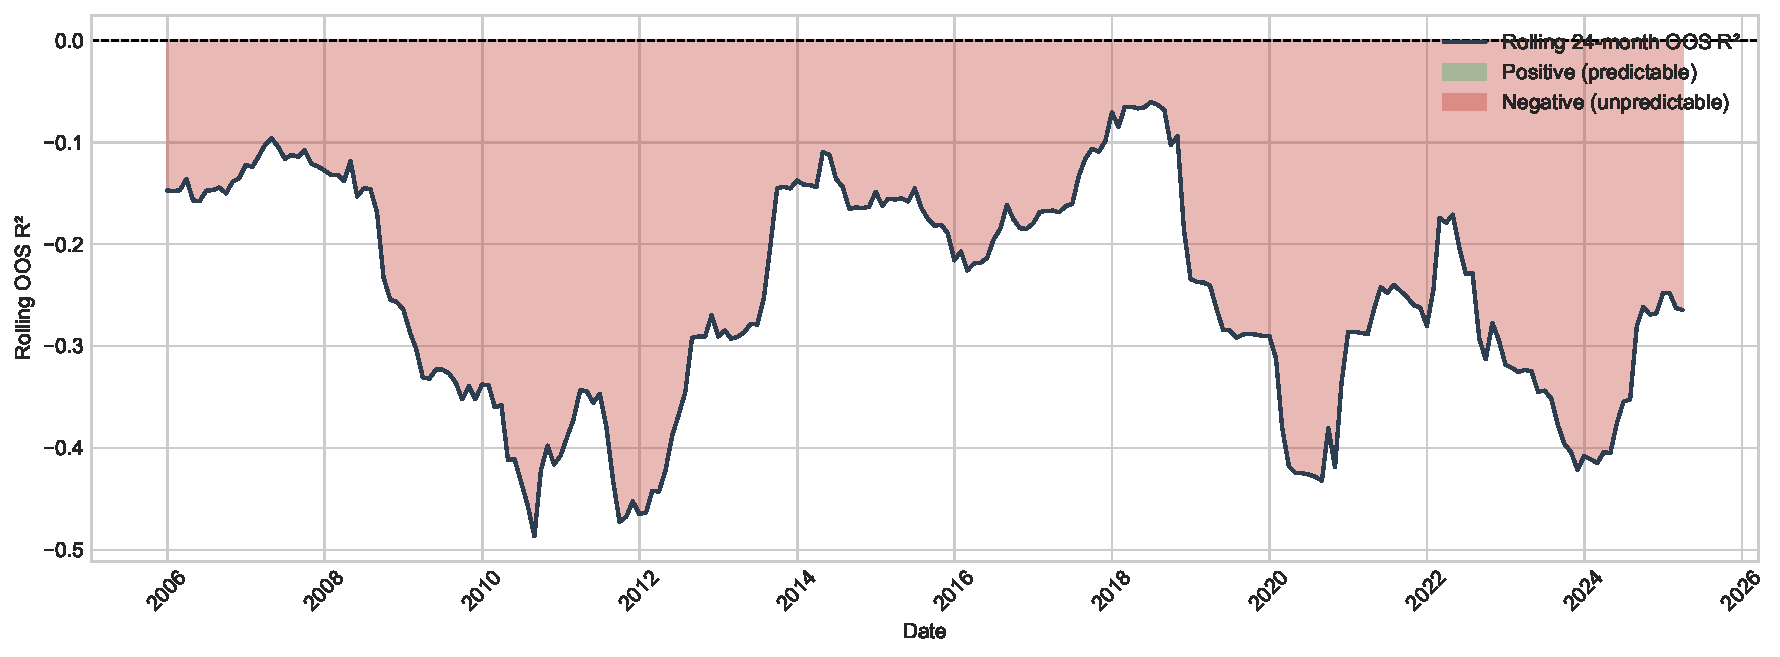
\includegraphics[width=0.7\linewidth]{files/aacae17f08c5853d36bc6047cc10ea6e.pdf}}
\label{fig-pockets}
\end{figure}

Figure~\ref{fig-pockets} reveals that predictability is far from uniform over time. There are clear \textbf{pockets} where the rolling OOS $R^2$ is sustainedly positive, and stretches where the model underperforms the naive cross-sectional mean. Several observations are worth noting:

\begin{itemize}
\item The pockets do not coincide trivially with known market regimes (bull/bear markets), suggesting that predictability has a complex relationship with economic conditions.
\item The transitions between predictable and unpredictable periods can be sharp, consistent with the structural-break interpretation in \cite{farmer2019pockets}.
\item The width of the window $W$ matters: a short window ($W=12$) reveals more erratic patterns; a long window ($W=48$) smooths out the signal but may miss shorter pockets.
\end{itemize}

This figure is the central empirical contribution of the chapter. It encapsulates the message that predictability should be thought of as a \textbf{dynamic property} of financial markets rather than a fixed parameter to be estimated.

\paragraph{The information coefficient through time}

The IC provides a complementary view by focusing on the \textbf{rank ordering} of returns rather than their magnitudes. A positive IC means the model successfully identifies which stocks will outperform; a negative IC means it systematically ranks them in the wrong order.

\begin{figure}[!htbp]
\centering
\begin{verbatim}
ic_series = pred_df['ic'].dropna()
ic_rolling = ic_series.rolling(12, center=True).mean()

fig, ax = plt.subplots(figsize=(12, 4))
ax.bar(ic_series.index, ic_series.values,
       color=['#27ae60' if v > 0 else '#c0392b' for v in ic_series.values],
       alpha=0.55, width=20, label='Monthly IC')
ax.plot(ic_rolling.index, ic_rolling.values,
        color='#0570EA', linewidth=1.8, label='12-month rolling mean')
ax.axhline(0,    color='black', linestyle='-',  linewidth=0.8)
ax.axhline( 0.05, color='grey',  linestyle='--', linewidth=0.8)
ax.axhline(-0.05, color='grey',  linestyle='--', linewidth=0.8)
ax.set_xlabel('Date')
ax.set_ylabel('Information Coefficient')
ax.xaxis.set_major_formatter(mdates.DateFormatter('%Y'))
ax.xaxis.set_major_locator(mdates.YearLocator(2))
plt.xticks(rotation=45)
ax.legend()
plt.tight_layout()
plt.show()

# Summary statistics
t_stat = ic_series.mean() / (ic_series.std() / np.sqrt(len(ic_series)))
pos_frac = (ic_series > 0).mean()
\end{verbatim}
\caption[]{\textbf{Information coefficient through time}: monthly IC (grey bars) and 12-month centred rolling average (blue line). The dashed lines mark IC = $\pm$0.05.

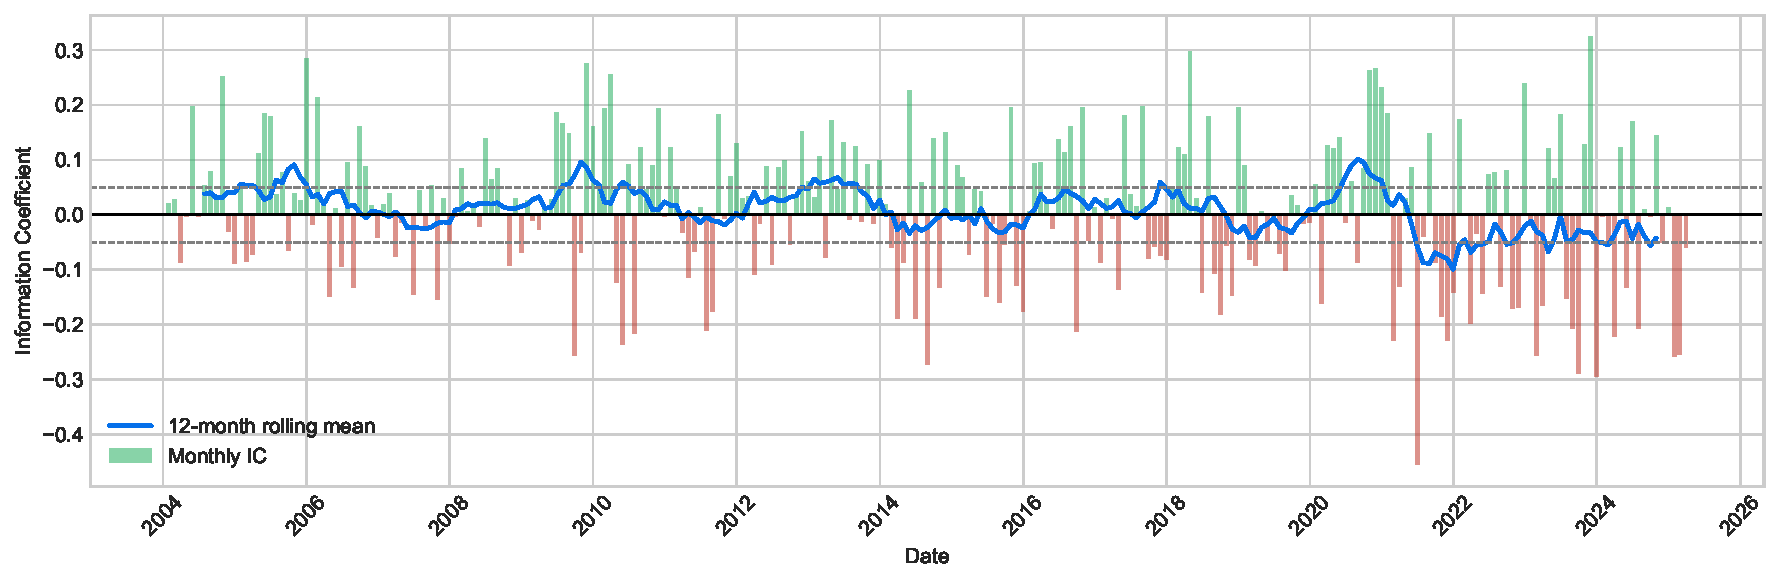
\includegraphics[width=0.7\linewidth]{files/da311d537f4f9e36398b56fb2b89c766.pdf}}
\label{fig-ic-time}
\end{figure}

\begin{verbatim}
print(f"Mean IC:         {ic_series.mean():.4f}")
print(f"Std IC:          {ic_series.std():.4f}")
print(f"t-statistic:     {t_stat:.2f}")
print(f"% positive months: {100*pos_frac:.1f}%")
\end{verbatim}

\begin{verbatim}
Mean IC:         0.0071
Std IC:          0.1302
t-statistic:     0.87
% positive months: 54.1%
\end{verbatim}

Figure~\ref{fig-ic-time} is best read alongside Figure~\ref{fig-pockets}. The IC fluctuates substantially from month to month, with persistent clusters of positive and negative values. The t-statistic on mean IC quantifies whether cross-sectional predictability is statistically significant on average. Periods with mean IC well above 0.05 correspond closely (though imperfectly) to the pockets identified through OOS $R^2$.

The fraction of months with positive IC is itself a useful diagnostic. Even a mean IC close to zero can deliver positive portfolio performance if the IC is positive in high-volatility months (when sorting errors are most costly) and negative in low-volatility months (when errors matter less). This observation underpins the \textbf{IC-Volatility adjusted} measures used in the systematic investing industry.

\paragraph{Feature-level predictability}

Predictability is not just heterogeneous over time: it also varies \textbf{across features}. Some characteristics (e.g., momentum) may be reliably predictive in trending markets but fare poorly in mean-reverting regimes. Others (e.g., value signals) may exhibit the opposite pattern. Decomposing the aggregate IC into feature-level contributions illuminates which parts of the signal are driving the pockets.

Below we compute, for each feature and each year, the average monthly IC of a univariate ridge regression using that feature alone.

\begin{verbatim}
# Feature-level IC by year
data_clean['year'] = data_clean['date'].dt.year
years  = sorted(data_clean['year'].unique())
feat_ic = {f: {} for f in features_short}

for f in features_short:
    cols_f = ['date', 'year', f, 'R1M']
    df_f = data_clean[cols_f].dropna().copy()
    df_f = df_f.sort_values('date')
    dates_f = sorted(df_f['date'].unique())

    ic_by_date = {}
    for i in range(min_train_months, len(dates_f)):
        train_d = dates_f[:i]
        test_d  = dates_f[i]
        train_f = df_f[df_f['date'].isin(train_d)]
        test_f  = df_f[df_f['date'] == test_d]
        if len(test_f) < min_test_stocks:
            continue
        X_tr = train_f[[f]].values
        y_tr = train_f['R1M'].values
        X_te = test_f[[f]].values
        y_te = test_f['R1M'].values
        mdl = Ridge(alpha=1.0)
        mdl.fit(X_tr, y_tr)
        ic_val, _ = spearmanr(y_te, mdl.predict(X_te))
        ic_by_date[test_d] = ic_val

    ic_s = pd.Series(ic_by_date)
    ic_s.index = pd.to_datetime(ic_s.index)
    ic_s_annual = ic_s.groupby(ic_s.index.year).mean()
    for yr, val in ic_s_annual.items():
        feat_ic[f][yr] = val

ic_heatmap = pd.DataFrame(feat_ic).T   # features \times years
# Keep only years with data for all features
ic_heatmap = ic_heatmap.dropna(axis=1, how='any')

print("Annual IC by feature (first 5 years):")
print(ic_heatmap.iloc[:, :5].round(3))
\end{verbatim}

\begin{verbatim}
Annual IC by feature (first 5 years):
                2004   2005   2006   2007   2008
Div_yld       -0.062  0.005 -0.041  0.040  0.006
EPS           -0.025  0.054  0.011 -0.004 -0.008
size_avg_252d  0.040  0.051  0.010 -0.011  0.036
mom_252       -0.014  0.073 -0.029  0.047  0.032
OCF_Growth_1Y -0.032 -0.021 -0.010  0.009  0.006
PB             0.051  0.015  0.041 -0.040 -0.024
vol_252       -0.037  0.073 -0.039  0.013 -0.072
\end{verbatim}

\begin{figure}[!htbp]
\centering
\begin{verbatim}
# Sort features by mean IC
feature_order = ic_heatmap.mean(axis=1).sort_values(ascending=False).index
ic_plot = ic_heatmap.loc[feature_order]

fig, ax = plt.subplots(figsize=(13, 4))
sns.heatmap(
    ic_plot,
    ax=ax,
    cmap='RdYlGn',
    center=0,
    vmin=-0.05,
    vmax=0.05,
    linewidths=0.4,
    linecolor='white',
    annot=False,
    cbar_kws={'label': 'Annual mean IC'}
)
ax.set_xlabel('Year')
ax.set_ylabel('Feature')
plt.xticks(rotation=45, fontsize=9)
plt.tight_layout()
plt.show()
\end{verbatim}
\caption[]{\textbf{Feature-level predictability}: annual average information coefficient by feature. Warm colours denote periods of positive IC; cool colours denote negative IC. Features are ordered by overall mean IC across the sample.

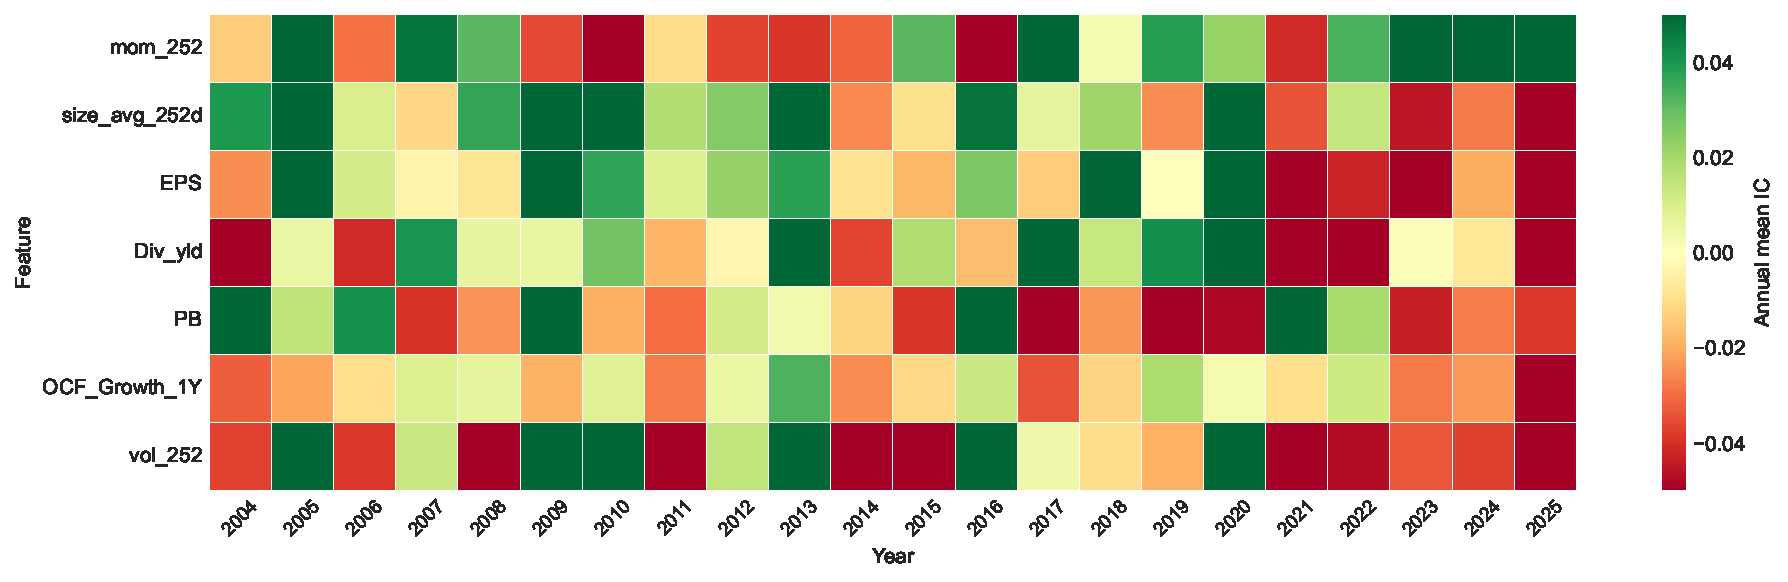
\includegraphics[width=0.7\linewidth]{files/675b62fe0bd6240813fad25d30074249.pdf}}
\label{fig-ic-heatmap}
\end{figure}

Figure~\ref{fig-ic-heatmap} makes the heterogeneity of predictability vivid. Several observations emerge:

\begin{itemize}
\item \textbf{No feature dominates uniformly}. Even the most predictive feature in aggregate has years of strongly negative IC. This corroborates the mosaic metaphor of \cite{cong2024mosaics}: assembling pieces from multiple sources yields a more stable signal than relying on any single characteristic.
\item \textbf{Momentum features} (e.g., \texttt{mom\_252}) tend to cluster: periods of positive IC for momentum features coincide, consistent with the idea that momentum payoffs are driven by common macroeconomic or sentiment factors.
\item \textbf{Value and quality signals} (e.g., \texttt{PB}, \texttt{OCF\_Growth\_1Y}) sometimes exhibit IC patterns that are out of phase with momentum, offering diversification potential at the feature level.
\item The pockets visible in Figure~\ref{fig-pockets} can often be traced to \textbf{synchronised positive IC} across multiple features. Conversely, the unpredictable stretches correspond to a mixture of negative and positive IC values that cancel when aggregated.
\end{itemize}

This analysis points to an important lesson for practitioners: evaluating features on the basis of their average IC alone is insufficient. One should examine the time-profile of IC and, ideally, condition on macro regimes. \cite{pesaran2024forecasting} formalise this within a panel forecasting framework, distinguishing between \textbf{parameter heterogeneity} (coefficients differ across units/periods) and \textbf{estimation uncertainty} (limited data inflates the variance of estimated coefficients), and show that the relative importance of these two sources varies substantially with horizon and sample size.

\paragraph{Cumulative OOS $R^2$ and investor value}

A complementary visualisation is the \textbf{cumulative OOS $R^2$}, which shows whether the model accumulates forecasting advantage over the full sample or whether periods of positive predictability are offset by negative ones.

\begin{figure}[!htbp]
\centering
\begin{verbatim}
# For each date t, compute: e_model^2 - e_baseline^2
# Cumulative sum shows when the model is ahead of the benchmark

records2 = []
for i in range(min_train_months, len(dates)):
    train_dates2 = dates[:i]
    test_date2   = dates[i]
    train2 = data_clean[data_clean['date'].isin(train_dates2)]
    test2  = data_clean[data_clean['date'] == test_date2]
    if len(test2) < min_test_stocks:
        continue
    X_tr2 = train2[features_short].values
    y_tr2 = train2['R1M'].values
    X_te2 = test2[features_short].values
    y_te2 = test2['R1M'].values
    m2 = Ridge(alpha=1.0)
    m2.fit(X_tr2, y_tr2)
    y_p2 = m2.predict(X_te2)
    mean_r = np.mean(y_te2)
    diff   = np.mean((y_te2 - mean_r)**2) - np.mean((y_te2 - y_p2)**2)
    records2.append({'date': test_date2, 'advantage': diff})

adv_df = pd.DataFrame(records2).set_index('date').sort_index()
cumadv  = adv_df['advantage'].cumsum()

fig, ax = plt.subplots(figsize=(12, 4))
ax.plot(cumadv.index, cumadv.values, color='#0570EA', linewidth=1.6)
ax.axhline(0, color='black', linestyle='--', linewidth=0.8)
ax.fill_between(cumadv.index, cumadv.values, 0,
                where=(cumadv.values >= 0), alpha=0.25, color='#27ae60')
ax.fill_between(cumadv.index, cumadv.values, 0,
                where=(cumadv.values <  0), alpha=0.25, color='#c0392b')
ax.set_xlabel('Date')
ax.set_ylabel('Cumulative model advantage')
ax.xaxis.set_major_formatter(mdates.DateFormatter('%Y'))
ax.xaxis.set_major_locator(mdates.YearLocator(2))
plt.xticks(rotation=45)
plt.tight_layout()
plt.show()
\end{verbatim}
\caption[]{\textbf{Cumulative OOS R\textsuperscript{2}}: accumulated difference in squared prediction errors between the ridge regression and the naive cross-sectional mean. Rising segments correspond to pockets where the model beats the benchmark.

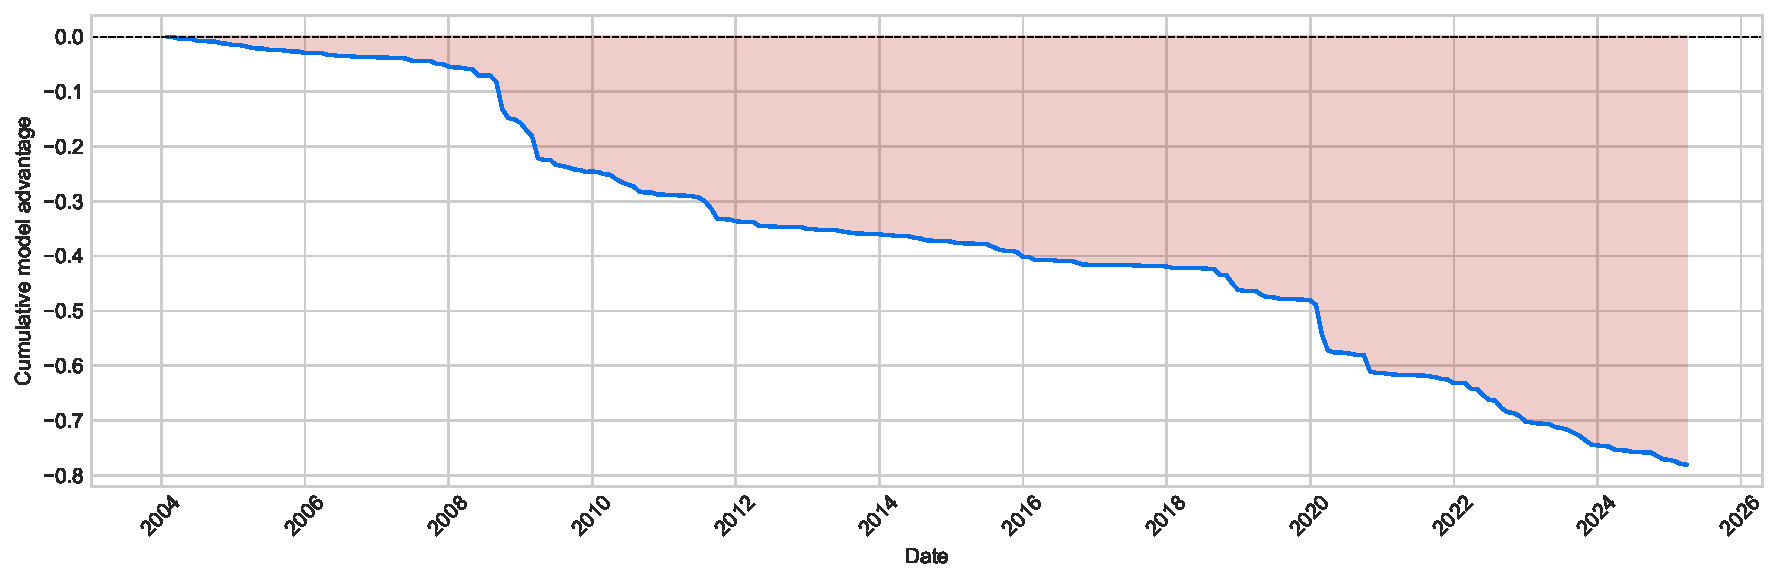
\includegraphics[width=0.7\linewidth]{files/cad258ae763d52f0ecb8558890043c37.pdf}}
\label{fig-cumoos}
\end{figure}

The cumulative chart is instructive in a different way from the rolling chart. If the cumulative advantage is monotonically increasing, the model is consistently better than the naive benchmark. If it oscillates around zero, gains and losses cancel. If it trends downward towards the end, the model has recently deteriorated (it seems so!). This picture is especially relevant for risk management: an investor who deployed the model would have accumulated gains in some periods, but also experienced drawdowns in others. The model is \textbf{not free} --- its value depends critically on the investor's ability to stay the course during unpredictable stretches.

\subsubsection{Predicting anomaly returns}\label{sec_pred_anomalies}

Most of the predictability literature takes individual stock returns as the quantity to be forecast. An alternative and increasingly influential approach is to forecast the \textbf{performance of strategies} --- i.e., the returns of long-short portfolios constructed on the basis of known anomalies. This ``meta-prediction'' framework asks: given that we know a particular anomaly (value, momentum, profitability...) has worked historically, can we predict \textit{when} it will work in the future?

\cite{bowles2024predicting} tackle this question systematically. They use a rich set of macro and market variables --- including uncertainty indicators, sentiment measures, and technical signals --- to forecast the returns of 93 equity anomalies. They find that anomaly returns are predictable to a meaningful degree: a strategy that overweights currently-predictable anomalies achieves a substantial Sharpe ratio improvement over naive equal-weighting.

This work connects naturally to the concept of \textbf{dynamic factor allocation}: rather than holding all factors at constant weights, tilting towards those most likely to deliver excess returns in the near future. The challenge, of course, is that predicting predictability is itself subject to overfitting --- and requires a rigorous OOS evaluation protocol of the kind advocated throughout this chapter.

\cite{singha2025discovery} push the idea further by investigating \textbf{regime-conditional} cross-sectional predictability. They document that the cross-sectional factor structure itself evolves through time via drift regimes, and that recognising these regimes unlocks predictability that is invisible to unconditional models. Their findings align with the drift-regime framework \cite{farmer2019pockets} use for time-series pockets, suggesting that regime-awareness is a unifying theme in modern predictability research.

The \cite{wang2025forecastability} paper contributes a useful prior step: measuring the \textbf{inherent forecastability} of a time series before any modelling is attempted. Using spectral entropy and Lyapunov exponents, they provide model-free measures of how predictable a given series is in principle. Applied to financial returns, such metrics can help triage which assets or anomalies are worth the modelling effort.

\subsubsection{Forecasting company fundamentals}\label{sec_pred_fundamentals}

A complementary approach to predicting returns directly is to forecast the \textbf{fundamental quantities} that drive valuations --- earnings, cash flows, profit margins --- and then derive return predictions from those forecasts through a valuation model. This two-stage approach has several potential advantages:

\begin{enumerate}
\item \textbf{Interpretability}: A model that first forecasts earnings and then derives a price target is more transparent than one that maps characteristics directly to returns.
\item \textbf{Stability}: Fundamental quantities may be more stationary than returns themselves, making them easier to model and reducing the risk of spurious patterns.
\item \textbf{Linkage to the real economy}: Macro forecasts, analyst estimates, and industry dynamics can be integrated more naturally into a fundamentals model.
\end{enumerate}

\cite{divo2025forecasting} investigate the use of modern ML tools --- including gradient-boosted trees and attention-based architectures --- to forecast earnings per share, return on equity, and revenue growth. They find substantial improvements over linear benchmarks, particularly for larger and more data-rich firms, and show that the forecastability of fundamentals is itself heterogeneous across industries and time.

\cite{cao2024fundamental} develop a comprehensive ML-based fundamental analysis framework. By training models on a broad set of accounting ratios and firm characteristics, they show that ML-based fundamental signals significantly outperform traditional analyst scores and accounting-based valuation ratios for predicting future returns. Their study is also careful to use an OOS evaluation protocol and to test robustness to transaction costs.

The forecasting literature on fundamentals has its own version of the pockets problem. \cite{pesaran2024forecasting} formalise this in a panel setting: when individual firms' parameters are heterogeneous (different firms respond differently to the same accounting signal), pooling all firms together in a single model introduces misspecification bias. They derive optimal forecasts that balance estimation efficiency (from pooling) against parameter heterogeneity (from keeping firm-specific models), providing a principled framework for practitioners deciding between pooled and firm-specific approaches.

A different decomposition is offered by \cite{lin2025market}, who work at the aggregate level. By separating market returns into dividend yield, earnings growth, and repricing components, they show that the predictable portion of the equity premium is concentrated in the repricing component --- consistent with the variance-decomposition insight of \cite{campbell2008predicting} and the canonical results of \cite{goyal2008comprehensive} on predictability concentrating in valuation-ratio driven components. Combining models tailored to each component yields OOS gains that are larger and more stable than those from a single aggregate predictor.

The cross-sectional analogue of return decomposition is \textbf{quantile prediction}. Rather than forecasting the mean return for each stock, one can target the \textbf{distribution} of returns, asking which stocks are more likely to appear in the top or bottom decile. \cite{uribe2025moving} pursue exactly this approach, using distributional regression to explain the tails of the cross-sectional return distribution with firm characteristics. Their results suggest that the tails are more predictable than the center, which has direct implications for tail-risk strategies and skewness tilts in portfolio construction.

\subsubsection{Comparing predictability across models}

A practical challenge is \textbf{how to statistically compare} the OOS performance of two competing forecasters. Classical tests of equal predictive accuracy --- such as the Diebold-Mariano test --- assume stationarity and may be poorly sized when predictions are generated from models estimated on overlapping samples. \cite{qu2023comparing} develop tests specifically designed for cross-sectional forecasting competitions, accounting for the fact that at each date the two models generate $N_t$ forecast-error pairs rather than a single pair. Their framework allows for heterogeneous and correlated errors across stocks, making it robust to the clustering of errors within industries or size groups.

This inferential framework is important because it guards against over-interpreting OOS differences. With a large cross-section, even tiny improvements in MSE are highly significant under conventional tests. \cite{qu2023comparing} provide corrections that yield better calibrated size while maintaining power, enabling more honest assessments of whether model improvements are genuinely exploitable.

The question of what makes a predictor \textit{consistently} better is also explored in \cite{cong2024mosaics} through the lens of \textbf{mosaic assembly}: combining a large number of individually weak predictors --- each associated with a specific data type, horizon, or stock segment --- into a mosaic that captures the full complexity of the cross-sectional return distribution. Their empirical results show that the mosaic approach dominates any single predictor and that the gains are not confined to a single pocket but persist across time, suggesting genuine diversification of the predictability sources.

\subsubsection{Conclusion}

Predictability in financial markets is neither a binary phenomenon (present or absent) nor a fixed parameter (constant over time). The evidence, both theoretical and empirical, points to a richer picture:

\begin{itemize}
\item \textbf{Pockets of predictability} are real: OOS $R^2$ and IC exhibit significant time variation, with stretches of genuine predictive accuracy interspersed with flat or negative performance. The rolling analyses in this chapter make this concrete on real equity data.
\item \textbf{Feature heterogeneity} matters: some signals work in some regimes and fail in others. A robust investment process monitors feature-level IC over time and reweights signals accordingly, rather than relying on average performance computed over the entire backtest.
\item \textbf{Strict OOS discipline is non-negotiable}. The failed replication attempt of \cite{cakici2025pockets} --- where a two-sided kernel allowed future information to contaminate forecasts --- underscores that even small implementation errors can create an illusion of predictability. All the results in this chapter are produced with a strict expanding-window protocol.
\item \textbf{Fundamentals and higher moments} extend the predictability frontier. Predicting company fundamentals (\cite{divo2025forecasting}, \cite{cao2024fundamental}) and the tails of the return distribution \citep{uribe2025moving} opens additional dimensions of predictability that the mean-return framework misses.
\end{itemize}

These conclusions have a direct impact on portfolio construction (Chapter \href{/chap-15-portfolio-backtesting}{Portfolio backtesting}): a strategy whose signal has time-varying predictability should dynamically adjust its confidence and hence its position sizing. This adaptive approach is, in a sense, the portfolio-management implementation of the statistical insight that predictability comes in pockets.

\subsubsection{Exercises}

\begin{enumerate}
\item \textbf{Window sensitivity}: Recompute Figure~\ref{fig-pockets} using rolling windows of 12, 36, and 48 months. How do the identified pockets change? Which window seems most useful for a practitioner who rebalances monthly?
\item \textbf{Model comparison}: Replace the ridge regression in the expanding-window loop with (a) a simple OLS regression and (b) an XGBoost model. Plot all three rolling OOS $R^2$ series on the same chart. Are the pockets model-specific or do they coincide across methods?
\item \textbf{Single-feature pockets}: Using the feature-level IC heatmap, identify the feature with the most persistent positive IC. Now compute its standalone rolling OOS $R^2$ and compare to the full-feature model. Does adding more features help or hurt during unpredictable periods?
\item \textbf{Hit ratio through time}: Compute the monthly hit ratio alongside the monthly OOS $R^2$ and IC. Do the three metrics agree on when the pockets occur? Compute their pairwise Pearson and Spearman correlations across months.
\item \textbf{Forecast combination}: At each forecast date, generate predictions from three univariate models (one per feature: \texttt{EPS}, \texttt{mom\_252}, \texttt{PB}). Compute a simple equal-weight combination of the three predictions and compare its rolling OOS $R^2$ to each individual model. Does combination reduce the depth of the negative (red) pockets?
\end{enumerate}

\subsection{Data preprocessing}

The methods we describe in this chapter are driven by financial applications. For an introduction to non-financial data processing, we recommend two references: chapter 3 from the general purpose ML book by \cite{boehmke2019hands} and the monograph on this dedicated subject by \cite{kuhn2019feature}.

\subsubsection{Setup and Imports}

\begin{verbatim}
import pandas as pd
import numpy as np
import matplotlib.pyplot as plt
import seaborn as sns
from scipy import stats
from statsmodels.tsa.stattools import acf
import warnings
warnings.filterwarnings('ignore')
# Set plotting style
plt.style.use('seaborn-v0_8-whitegrid')
sns.set_palette("husl")

# Building the data & import functions
from data_build import generate_data
from data_build import plot_conditional_expectations
from data_build import compute_correlations_with_label
from data_build import compute_autocorrelations
data_ml, features, features_short, returns, stock_ids, stock_ids_short = generate_data()
features_short =["Div_yld", "EPS", "size_avg_252d", "mom_252", "OCF_Growth_1Y", "PB", "vol_252"]
\end{verbatim}

\subsubsection{Know your data}

The first step, as in any quantitative study, is obviously to make sure the data is trustworthy, i.e., comes from a reliable provider (a minima). The landscape in financial data provision is vast to say the least: some providers are well established (e.g., Bloomberg, Thomson-Reuters, Datastream, CRSP, Morningstar), some are more recent (e.g., Capital IQ, Ravenpack) and some focus on alternative data niches (see \href{https://alternativedata.org/data-providers/}{https://alternativedata.org/data-providers/} for an exhaustive list). Unfortunately, and to the best of our knowledge, no study has been published that evaluates a large spectrum of these providers in terms of data reliability.

The second step is to have a look at \textbf{summary statistics}: ranges (minimum and maximum values), and averages and medians. Histograms or plots of time series carry of course more information but cannot be analyzed properly in high dimensions. They are nonetheless sometimes useful to track local patterns or errors for a given stock and/or a particular feature.
Beyond first order moments, second order quantities (variances and covariances/correlations){\textbackslash}index\{correlation\} also matter because they help spot colinearities. When two features are highly correlated, problems may arise in some models (e.g., simple regressions, see Section~\ref{corpred}).

Often, the number of predictors is so large that it is unpractical to look at these simple metrics. A minimal verification is recommended. To further ease the analysis:

\begin{itemize}
\item focus on a subset of predictors, e.g., the ones linked to the most common factors (market-capitalization, price-to-book or book-to-market, momentum (past returns), profitability, asset growth, volatility);
\item track outliers in the summary statistics (when the maximum/median or median/minimum ratios seem suspicious).
\end{itemize}

Below, in Figure~\ref{fig-correl_label}, we show a box plot that illustrates the distribution of correlations{\textbackslash}index\{correlation\} between features and the one month ahead return. The correlations are computed on a date-by-date basis, over the whole cross-section of stocks. They are mostly located close to zero, but some dates seem to experience extreme shifts (outliers are shown with black circles). The market capitalization has the median which is the most negative while volatility is the only predictor with positive median correlation (this particular example seems to refute the low risk anomaly).

\paragraph{Boxplot of correlations with the 1M forward return (label)}

\begin{figure}[!htbp]
\centering
\begin{verbatim}
corr_data = compute_correlations_with_label(data_ml, features_short)
fig, ax = plt.subplots(figsize=(10, 6))
sns.boxplot(data=corr_data, x='correlation', y='Predictor', hue='Predictor', legend=False,
            palette='husl', flierprops={'marker': 'o', 'markerfacecolor': 'black'})
ax.set_xlabel('Correlation with R1M')
ax.set_ylabel('')
ax.set_aspect(0.05)
plt.tight_layout()
plt.show()
\end{verbatim}
\caption[]{Boxplot of correlations with the 1M forward return (label).

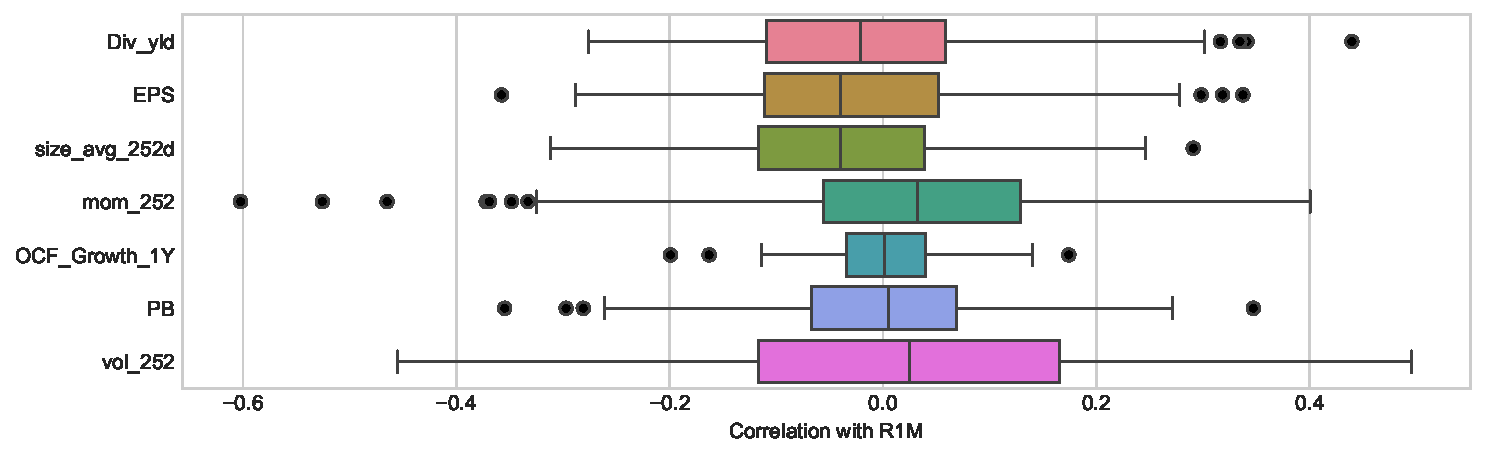
\includegraphics[width=0.7\linewidth]{files/d5daafb94fec82ee7f1e41e06fa7a8ca.pdf}}
\label{fig-correl_label}
\end{figure}

More importantly, when seeking to work with supervised learning (as we will do most of the time), the link of some features with the dependent variable can be further characterized by the smoothed \textbf{conditional average}{\textbackslash}index\{conditional average\} because it shows how the features impact the label. The use of the conditional average has a deep theoretical grounding. Suppose there is only one feature $X$ and that we seek a model $Y=f(X)+\text{error}$, where variables are real-valued. The function $f$ that minimizes the average squared error $\mathbb{E}[(Y -f(X))^2]$ is the so-called regression function (see Section 2.4 in \cite{friedman2009elements}):

\begin{equation}
\label{regfun}
f(x)=\mathbb{E}[Y|X=x].
\end{equation}

In \ref{regfun}, we plot two illustrations of this function when the dependent variable ($Y$) is the one month ahead return. The first one pertains to the average market capitalization over the past year and the second to the volatility over the past year as well. Both predictors have been uniformized (see Section~\ref{scaling} below) so that their values are uniformly distributed in the cross-section of assets for any given time period. Thus, the range of features is $[0,1]$ and is shown on the $x$-axis of the plot. The grey corridors around the lines show 95\% level confidence interval for the computation of the mean. Essentially, it is narrow when both (i) many data points are available and (ii) these points are not too dispersed.

\begin{figure}[!htbp]
\centering
\begin{verbatim}
plot_conditional_expectations(data_ml, ['size_avg_252d', 'vol_252'])
\end{verbatim}
\caption[]{Conditional expectations: average returns as smooth functions of features.

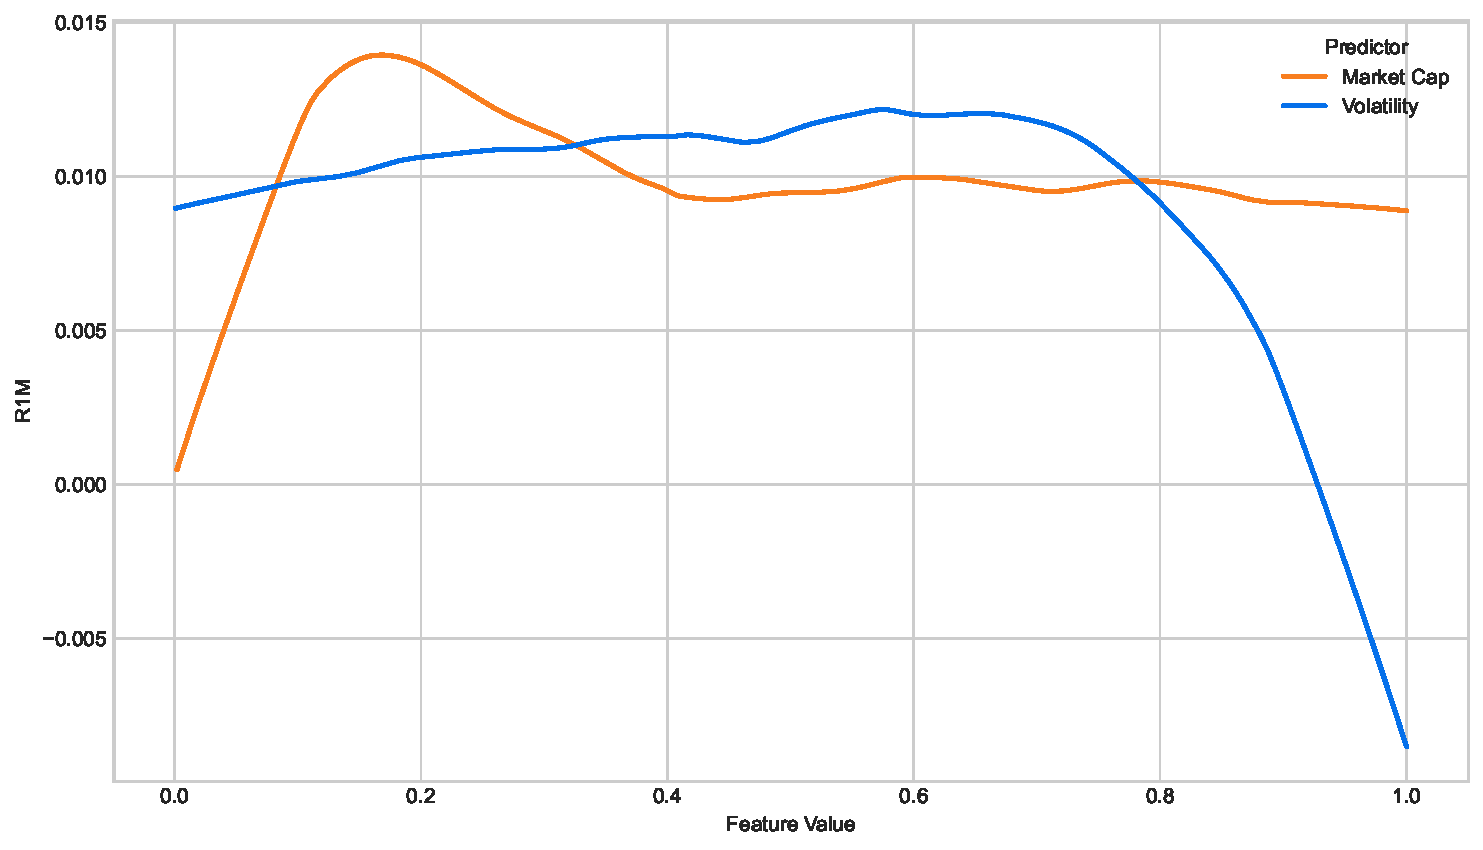
\includegraphics[width=0.7\linewidth]{files/1566510201c4a673d3e9d73423f3a31e.pdf}}
\label{fig-cond_exp}
\end{figure}

The two variables do not have a monotonic impact on future returns. Overall, returns, on average, increase with market capitalization (thereby contradicting the so-called \textit{size} effect). The reverse pattern is observed for volatility: the curve is rather flat for the first half of volatility scores and then decreases, especially over the last quintile of volatility values (thereby corroborating the low-volatility anomaly).

One important empirical property of features is \textbf{autocorrelation}{\textbackslash}index\{autocorrelation\} (or absence thereof). A high level of autocorrelation for one predictor makes it plausible to use simple imputation techniques when some data points are missing. But autocorrelation is also important when moving towards prediction tasks and we discuss this issue shortly below in Section~\ref{pers}. In Figure @ref(fig:histcorr), we build the histogram of autocorrelations, computed stock-by-stock and feature-by-feature.

\begin{figure}[!htbp]
\centering
\begin{verbatim}
autocorrs = compute_autocorrelations(data_ml, features)

fig, ax = plt.subplots(figsize=(8, 5))
ax.hist(autocorrs['acf'], bins=60, edgecolor='white')
ax.set_xlim(-0.1, 1)
ax.set_xlabel('Autocorrelation')
ax.set_ylabel('Frequency')
plt.tight_layout()
plt.show()
\end{verbatim}
\caption[]{Histogram of feature autocorrelations.

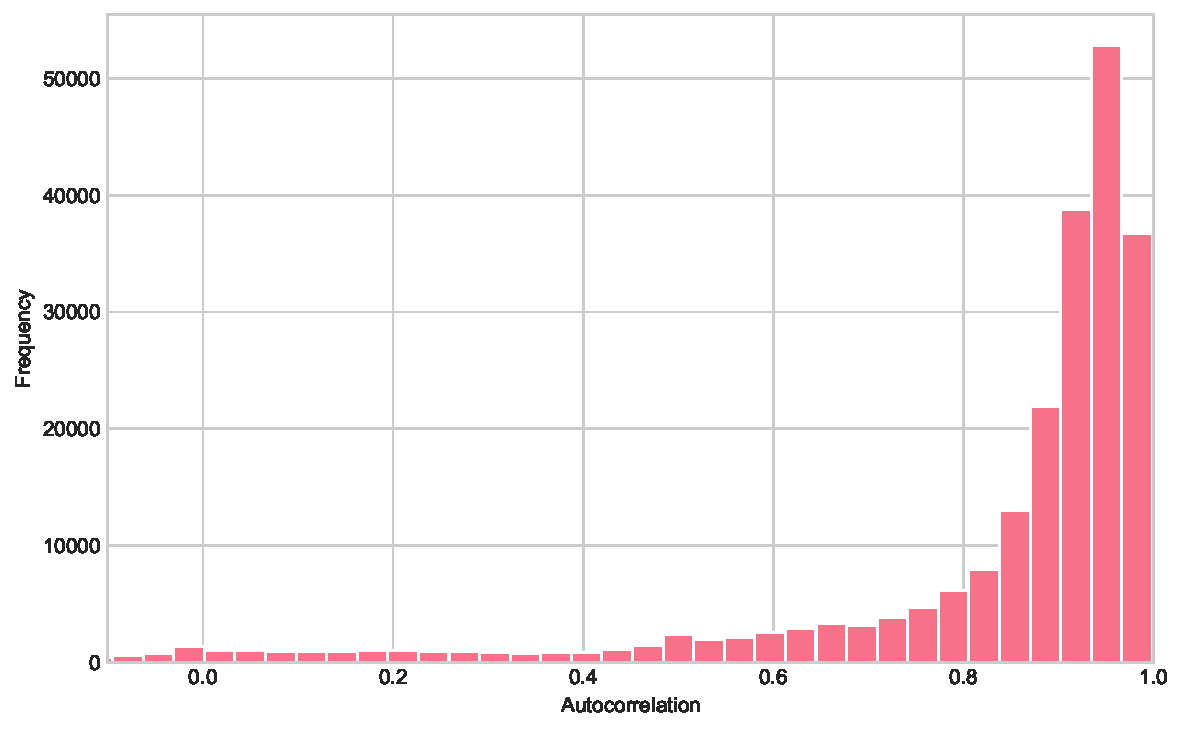
\includegraphics[width=0.7\linewidth]{files/02df7013196e26b27ddca97860ee68ed.pdf}}
\label{fig-autocorr}
\end{figure}

Given the large number of values to evaluate, the above chunk is quite time-consuming. The output shows that predictors are highly autocorrelated: most of them have a first order autocorrelation above 0.80.

\subsubsection{Missing data}

Similarly to any empirical discipline, portfolio management is bound to face missing data issues. The topic is well known and several books detail solutions to this problem (e.g., \cite{allison2001missing}, \cite{enders2010applied}, \cite{little2014statistical} and \cite{van2018flexible}). While researchers continuously propose new methods to cope with absent points (\cite{honaker2010missing} or \cite{che2018recurrent} to cite but a few), we believe that a simple, heuristic treatment is usually sufficient as long as some basic cautious safeguards are enforced.

First of all, there are mainly two ways to deal with missing data: \textbf{removal} and \textbf{imputation}. Removal is agnostic but costly, especially if one whole instance is eliminated because of only one missing feature value. Imputation{\textbackslash}index\{imputation\}{\textbackslash}index\{data imputation\} is often preferred but relies on some underlying and potentially erroneous assumption.

A simplified classification of imputation is the following:

\begin{itemize}
\item A basic imputation choice is the median (or mean) of the feature for the stock over the past available values. If there is a trend in the time series, this will nonetheless alter the trend. Relatedly, this method can be forward-looking, unless the training and testing sets are treated separately.
\item In time series contexts with views towards backtesting, the most simple imputation comes from previous values: if $x_t$ is missing, replace it with $x_{t -1}$. This makes sense most of the time because past values are all that is available and are by definition backward-looking. However, in some particular cases, this may be a very bad choice (see words of caution below).
\item Medians and means can also be computed over the \textbf{cross-section} of assets. This roughly implies that the missing feature value will be relocated in the bulk of observed values. When many values are missing, this creates an atom in the distribution of the feature and alters the original distribution. One advantage is that this imputation is not forward-looking.
\item Many techniques rely on some modelling assumptions for the data generating process. We refer to nonparametric approaches (\cite{stekhoven2011missforest} and \cite{shah2014comparison}, which rely on random forests, see Chapter \href{/chap-07-trees}{Tree-based methods}), Bayesian imputation \citep{schafer1999multiple}, maximum likelihood approaches (\cite{enders2001primer}, \cite{enders2010applied}), interpolation or extrapolation and nearest neighbor algorithms \citep{garcia2009k}. More generally, the four books cited at the begining of the subsection detail many such imputation processes. Advanced techniques are much more demanding computationally.
\item Three recent papers examine this question closely. \cite{chen2024missing} find that plain cross sectional mean imputation rivals expectation maximization, since missing values cluster in blocks with little cross sectional signal. \cite{freyberger2025missing} cast imputation as weighted least squares within a generalized method of moments framework, keeping every observed return while ensuring valid inference. \cite{bryzgalova2025missing} show missingness is pervasive and systematic, and build a method that exploits both time and cross sectional structure. The first paper offers the clearest and most practical take.
\end{itemize}

A few words of caution:

\begin{itemize}
\item Interpolation should be avoided \textbf{at all cost}. Accounting values or ratios that are released every quarter must never be linearly interpolated for the simple reason that this is forward-looking. If numbers are disclosed in January and April, then interpolating February and March requires the knowledge of the April figure, which, in live trading will not be known. Resorting to past values is a better way to go.
\item Nevertheless, there are some feature types for which imputation from past values should be avoided. First of all, returns should not be replicated. By default, a superior choice is to set missing return indicators to zero (which is often close to the average or the median). A good indicator that can help the decision is the persistence of the feature through time. If it is highly autocorrelated (and the time series plot create a smooth curve, like for market capitalization), then imputation from the past can make sense. If not, then it should be avoided.
\item There are some cases that can require more attention. Let us consider the following fictitious sample of dividend yield:
\end{itemize}

\bigskip\noindent
\begin{tabular}{p{\dimexpr 0.333\linewidth-2\tabcolsep}p{\dimexpr 0.333\linewidth-2\tabcolsep}p{\dimexpr 0.333\linewidth-2\tabcolsep}}
\toprule
Date & Original yield & Replacement value \\
\hline
2015-02 & NA & preceding (if it exists) \\
2015-03 & 0.02 & untouched (none) \\
2015-04 & NA & 0.02 (previous) \\
2015-05 & NA & 0.02 (previous) \\
2015-06 & NA & \textless = \textbf{Problem}! \\
\bottomrule
\end{tabular}

\bigskip

In this case, the yield is released quarterly, in March, June, September, etc. But in June, the value is missing. The problem is that we cannot know if it is missing because of a genuine data glitch, or because the firm simply did not pay any dividends in June. Thus, imputation from past value may be erroneous here. There is no perfect solution but a decision must nevertheless be taken. For dividend data, three options are:

\begin{enumerate}
\item Keep the previous value. In R, the function na.locf() from the \textit{zoo} package is incredibly efficient for this task.
\item Extrapolate from previous observations (this is very different from \textbf{inter}polation): for instance, evaluate a trend on past data and pursue that trend.
\item Set the value to zero. This is tempting but may be sub-optimal due to dividend smoothing practices from executives (see for instance \cite{leary2011determinants} and \cite{chen2012dividend} for details on the subject). For persistent time series, the first two options are probably better.
\end{enumerate}

Tests can be performed to evaluate the relative performance of each option. It is also important to \textbf{remember} these design choices. There are so many of them that they are easy to forget. Keeping track of them is obviously compulsory. In the ML pipeline, the \textbf{scripts} pertaining to data preparation are often key because they do not serve only once!

Finally, we recall that core librairies in python such as \href{https://scikit-learn.org/stable/}{scikit-learn}, \href{https://pandas.pydata.org/}{pandas} and \href{https://www.statsmodels.org/stable/index.html}{statsmodels} have functions dedicated to imputation: that deal with data imputation: \textit{SimpleImputer}, \textit{KNNImputer}, \textit{IterativeImputer}, \textit{fillna}. The interested reader can have a look at these.

Below, we provide example of custom functions that implement the forward-filling and cross-sectional imputation. Note that the latter must be performed on a data-by-date basis. This is to avoid any forward-looking leakage.

\begin{verbatim}
def forward_fill_imputation(df, columns):
    """
    Impute missing values using forward fill (previous value).
    Equivalent to R's zoo::na.locf()
    """
    df_imputed = df.copy()
    df_imputed[columns] = df_imputed[columns].ffill()
    return df_imputed

def cross_sectional_median_imputation(df, columns, date_col='date'):
    """
    Impute missing values using cross-sectional median for each date.
    """
    df_imputed = df.copy()
    for col in columns:
        df_imputed[col] = df_imputed.groupby(date_col)[col].transform(
            lambda x: x.fillna(x.median())
        )
    return df_imputed
\end{verbatim}

\subsubsection{Outlier detection}

The topic of outlier detection{\textbackslash}index\{outlier detection\} is also well documented and has its own surveys (\cite{hodge2004survey}, \cite{chandola2009anomaly} and \cite{gupta2014outlier}) and a few dedicated books (\cite{aggarwal2013outlier} and \cite{rousseeuw2005robust}, though the latter is very focused on regression analysis).

Again, incredibly sophisticated methods may require a lot of efforts for possibly limited gain. Simple heuristic methods, as long as they are documented in the process, may suffice. They often rely on `hard' thresholds:

\begin{itemize}
\item for one given feature (possibly filtered in time), any point outside the interval $[\mu -m\sigma, \mu+m\sigma]$ can be deemed an outlier. Here $\mu$ is the mean of the sample and $\sigma$ the standard deviation. The multiple value $m$ usually belongs to the set $\{3, 5, 10\}$, which is of course arbitrary.
\item likewise, if the largest value is above $m$ times the second-to-largest, then it can also be classified as an outlier (the same reasoning applied for the other side of the tail).
\item finally, for a given small threshold $q$, any value outside the $[q,1 -q]$ quantile range can be considered outliers.
\end{itemize}

This latter idea was popularized by \textbf{winsorization}.{\textbackslash}index\{winsorization\} Winsorizing amounts to setting to $x^{(q)}$ all values below $x^{(q)}$ and to $x^{(1 -q)}$ all values above $x^{(1 -q)}$. The winsorized variable $\tilde{x}$ is:
\begin{equation}
\tilde{x}_i=\left\{\begin{array}{ll}
x_i & \text{ if }  x_i \in [x^{(q)},x^{(1-q)}] \quad \text{ (unchanged)}\\
x^{(q)} & \text{ if }  x_i < x^{(q)} \\
x^{(1-q)} & \text{ if }  x_i > x^{(1-q)}
 \end{array} \right. .
\end{equation}

The range for $q$ is usually $(0.5\%, 5\%)$ with 1\% and 2\% being the most often used.

The winsorization stage \textbf{must} be performed on a feature-by-feature and a date-by-date basis. However, keeping a time series perspective is also useful. For instance, a \$800B market capitalization may seems out of range, except when looking at the history of Apple's capitalization.

We conclude this subsection by recalling that \textit{true} outliers (i.e., extreme points that are not due to data extraction errors) are valuable because they are likely to carry important information. We also provide two examples for winsorization.

\begin{verbatim}
def winsorize(series, q=0.01):
    lower = series.quantile(q)
    upper = series.quantile(1 - q)
    return series.clip(lower=lower, upper=upper)

def winsorize_by_date(df, columns, date_col='date', q=0.01):
    df_winsorized = df.copy()
    for col in columns:
        df_winsorized[col] = df_winsorized.groupby(date_col)[col].transform(
            lambda x: winsorize(x, q)
        )
    return df_winsorized
\end{verbatim}

\subsubsection{Feature engineering}\label{feateng}

Feature engineering{\textbackslash}index\{feature engineering\} is a very important step of the portfolio construction process. Computer scientists often refer to the saying ``\textit{garbage in, garbage out}''. It is thus paramount to prevent the ML engine of the allocation to be trained on ill-designed variables.
We invite the interested reader to have a look at the recent work of \cite{kuhn2019feature} on this topic. The (shorter) academic reference is \cite{guyon2003introduction}.

\paragraph{Feature selection}

The first step is selection. It is not obvious to determine which set of predictors to include. For instance, \cite{bali2020cross} show that fixed-income related variables do not help to predict equity returns. One heuristic choice is to chose the variables that are often mentioned in the literature (both academic and practical). Though of course, sticking to common characteristics may complicate the generation of alpha because all trading agents will take them into account. Choices can stem from empirical studies such as \cite{chen2021open}, or theoretical models like \cite{ohlson1995earnings}, which is one of the many papers that justify the inclusion of fundamental values as independent variables in predictive models.

Then, given a large set of predictors, it seems a sound idea to filter out unwanted or redundant exogenous variables. Heuristically, simple methods include:

\begin{itemize}
\item computing the correlation matrix of all features and making sure that no (absolute) value is above a threshold (0.7 is a common value) so that redundant variables do not pollute the learning engine;
\item carrying out a linear regression and removing the non significant variables (e.g., those with $p$-value above 0.05).
\item perform a clustering analysis over the set of features and retain only one feature within each cluster (see Chapter \href{/chap-21-unsupervised}{Unsupervised learning}).
\end{itemize}

Both these methods are somewhat reductive and overlook nonlinear relationships. Another approach would be to fit a decision tree (or a random forest) and retain only the features that have a high variable importance. These methods will be developed in Chapter \href{/chap-07-trees}{Tree-based methods} for trees and Chapter \href{/chap-19-interpretability}{Interpretability} for variable importance.

\paragraph{Scaling the predictors}\label{scaling}

{\textbackslash}index\{scaling methods\}

The premise of the need to pre-process the data comes from the large variety of scales in financial data:

\begin{itemize}
\item returns are most of the time smaller than one in absolute value;
\item stock volatility lies usually between 5\% and 80\%;
\item market capitalization is expressed in million or billion units of a particular currency;
\item accounting values as well;
\item accounting ratios can have inhomogeneous units;
\item synthetic attributes like sentiment also have their idiosyncrasies.
\end{itemize}

While it is widely considered that monotonic transformations of the features have a marginal impact on prediction outcomes, \cite{galili2016splitting} show that this is not always the case (see also Section @ref(impact-of-rescaling-toy-example)). Hence, the choice of normalization may in fact very well matter.

If we write $x_i$ for the raw input and $\tilde{x}_i$ for the transformed data, common scaling practices include: {\textbackslash}index\{standardization\}

\begin{itemize}
\item \textbf{standardization}: $\tilde{x}_i=(x_i -m_x)/\sigma_x$, where $m_x$ and $\sigma_x$ are the mean and standard deviation of $x$, respectively;
\item \textbf{min-max} rescaling over [0,1]: $\tilde{x}_i=(x_i -\min(\mathbf{x}))/(\max(\mathbf{x}) -\min(\mathbf{x}))$;
\item \textbf{min-max} rescaling over [-1,1]: $\tilde{x}_i=2\frac{x_i -\min(\mathbf{x})}{\max(\mathbf{x}) -\min(\mathbf{x})} -1$;
\item \textbf{uniformization}:{\textbackslash}index\{uniformization\} $\tilde{x}_i=F_\mathbf{x}(x_i)$, where $F_\mathbf{x}$ is the empirical c.d.f. of $\mathbf{x}$. In this case, the vector $\tilde{\mathbf{x}}$ is defined to follow a uniform distribution over [0,1].
\end{itemize}

Sometimes, it is possible to apply a logarithmic transform of variables with both large values (market capitalization) and large outliers. The scaling can come after this transformation. Obviously, this technique is prohibited for features with negative values.

It is often advised to scale inputs so that they range in [0,1] before sending them through the training of neural networks for instance. The dataset that we use in this book is based on variables that have been uniformized: for each point in time, the cross-sectional distribution of each feature is uniform over the unit interval. In factor investing, the scaling of features must be \textbf{operated separately for each date and each feature}. This point is critical. It makes sure that for every rebalancing date, the predictors will have a similar shape and do carry information on the cross-section of stocks.

Uniformization is sometimes presented differently: for a given characteristic and time, characteristic values are ranked and the rank is then divided by the number of non-missing points. This is done in \cite{freyberger2020dissecting} for example. In \cite{kelly2019characteristics}, the authors perform this operation but then subtract 0.5 to all features so that their values lie in [-0.5,0.5].

Scaling features across dates should be proscribed. Take for example the case of market capitalization. In the long run (market crashes notwithstanding), this feature increases through time. Thus, scaling across dates would lead to small values at the beginning of the sample and large values at the end of the sample. This would completely alter and dilute the cross-sectional content of the features.  {\textbackslash}index\{scaling methods\}

\begin{verbatim}
def norm_unif(v):
    """
    Uniformize a vector using the empirical CDF.
    Values are transformed to follow a uniform distribution over [0,1].
    """
    return stats.rankdata(v, method='average') / len(v)

def norm_0_1(v):
    """
    Min-max rescaling to [0,1] interval.
    """
    v = np.array(v)
    return (v - v.min()) / (v.max() - v.min())

def standardize(v):
    """
    Standardization: (x - mean) / std
    """
    v = np.array(v)
    return (v - v.mean()) / v.std()
\end{verbatim}

\subsubsection{Labelling}

\paragraph{Simple labels}

{\textbackslash}index\{labelling\}
There are several ways to define labels when constructing portfolio policies. Of course, the finality is the portfolio weight, but it is rarely considered as the best choice for the label. Some methodologies do map firm attributes into final weights, e.g., \cite{brandt2009parametric} and \cite{ammann2016characteristics}, but these are outside the scope of the book.

Usual labels in factor investing are the following:

\begin{itemize}
\item raw asset returns;
\item future relative returns (versus some benchmark: market-wide index, or sector-based portfolio for instance). One simple choice is to take returns minus a cross-sectional mean or median;
\item the probability of positive return (or of return above a specified threshold);
\item the probability of outperforming a benchmark (computed over a given time frame);
\item the binary version of the above: YES (outperforming) versus NO (underperforming);
\item risk-adjusted versions of the above: Sharpe ratios, information ratios, MAR or CALMAR ratios (see Section @ref(perfmet)).
\end{itemize}

When creating binary variables, it is often tempting to create a test that compares returns to zero (profitable versus non profitable). This is not optimal because it is very much time-dependent. In good times, many assets will have positive returns, while in market crashes, few will experience positive returns, thereby creating very unbalanced classes. It is a better idea to split the returns in two by comparing them to their time-$t$ median (or average). In this case, the indicator is relative and the two classes are much more balanced.

As we will discuss later in this chapter, these choices still leave room for additional degrees of freedom. Should the labels be rescaled, just like features are processed? What is the best time horizon on which to compute performance metrics?

\paragraph{Categorical labels}

{\textbackslash}index\{categorical labels\}
In a typical ML analysis, when $y$ is a proxy for future performance, the ML engine will try to minimize some distance between the predicted value and the realized values. For mathematical convenience, the sum of squared error ($L^2$ norm) is used because it has the simplest derivative and makes gradient descent accessible and easy to compute.

Sometimes, it can be interesting not to focus on raw performance proxies, like returns or Sharpe ratios, but on discrete investment decisions, which can be derived from these proxies. A simple example (decision rule) is the following:

\begin{equation}
\label{catlabel}
y_{t,i}=\left\{  \begin{array}{rll}
-1 & \text{ if } & \hat{r}_{t,i} < r_- \\
0 & \text{ if } & \hat{r}_{t,i} \in [r_-,r_+] \\
+1 & \text{ if } & \hat{r}_{t,i} > r_+ \\
\end{array} \right.,
\end{equation}
where $\hat{r}_{t,i}$ is the performance proxy (e.g., returns or Sharpe ratio) and $r_\pm$ are the decision thresholds. When the predicted performance is below $r_ -$, the decision is -1 (e.g., \textit{sell}), when it is above $r_+$, the decision is +1 (e.g., \textit{buy}) and when it is in the middle (the model is neither very optimistic nor very pessimistic), then the decision is neutral (e.g., \textit{hold}). The performance proxy can of course be relative to some benchmark so that the decision is directly related to this benchmark. It is often advised that the thresholds $r_\pm$ be chosen such that the three categories are relatively balanced, that is, so that they end up having a comparable number of instances.

In this case, the final output can be considered as categorical or numerical because it belongs to an important subgroup of categorical variables: the ordered categorical (\textbf{ordinal}) variables.{\textbackslash}index\{ordinal variable\} If $y$ is taken as a number, the usual regression tools apply.

When $y$ is treated as a non-ordered (\textbf{nominal}) categorical variable,{\textbackslash}index\{nominal variable\} then a new layer of processing is required because ML tools only work with numbers. Hence, the categories must be recoded into digits. The mapping that is most often used is called `\textbf{one-hot encoding}'.{\textbackslash}index\{one-hot encoding\} The vector of classes is split in a sparse matrix in which each column is dedicated to one class. The matrix is filled with zeros and ones. A one is allocated to the column corresponding to the class of the instance. We provide a simple illustration in the table below.

\bigskip\noindent
\begin{tabular}{p{\dimexpr 0.250\linewidth-2\tabcolsep}p{\dimexpr 0.250\linewidth-2\tabcolsep}p{\dimexpr 0.250\linewidth-2\tabcolsep}p{\dimexpr 0.250\linewidth-2\tabcolsep}}
\toprule
Initial data &  & One-hot encoding &  \\
\hline
Position & Sell & Hold & Buy \\
buy & 0 & 0 & 1 \\
buy & 0 & 0 & 1 \\
hold & 0 & 1 & 0 \\
sell & 1 & 0 & 0 \\
buy & 0 & 0 & 1 \\
\bottomrule
\end{tabular}

\bigskip

In classification tasks,{\textbackslash}index\{classification\} the output has a larger dimension. For each instance, it gives the probability of belonging to each class assigned by the model. As we will see in Chapters \href{/chap-07-trees}{Tree-based methods} and @ref(NN), this is easily handled via the softmax function.

From the standpoint of allocation, handling categorical predictions is not necessarily easy. For long-short portfolios, plus or minus one signals can provide the sign of the position. For long-only portfolio, two possible solutions: (i) work with binary classes (in versus out of the portfolio) or (ii) adapt weights according to the prediction: zero weight for a -1 prediction, 0.5 weight for a 0 prediction and full weight for a +1 prediction. Weights are then of course normalized so as to comply with the budget constraint.

\paragraph{The triple barrier method}

We conclude this section with an advanced labelling technique mentioned in \cite{de2018advances}. The idea is to consider the full dynamics of a trading strategy and not a simple performance proxy. The rationale for this extension is that often money managers implement P\&L triggers that cash in when gains are sufficient or opt out to stop their losses. Upon inception of the strategy, three barriers are fixed (see Figure @ref(fig:triplebarrier)):

\begin{itemize}
\item one above the current level of the asset (magenta line), which measures a reasonable expected profit;
\item one below the current level of the asset (cyan line), which acts as a stop-loss signal to prevent large negative returns;
\item and finally, one that fixes the horizon of the strategy after which it will be terminated (black line).
\end{itemize}

If the strategy hits the first (\textit{resp}. second) barrier, the output is +1 (\textit{resp}. -1), and if it hits the last barrier, the output is equal to zero or to some linear interpolation (between -1 and +1) that represents the position of the terminal value relative to the two horizontal barriers. Computationally, this method is \textbf{much} more demanding, as it evaluates a whole trajectory for each instance. Again, it is nonetheless considered as more realistic because trading strategies are often accompanied with automatic triggers such as stop-loss, etc.

\begin{figure}[!htbp]
\centering
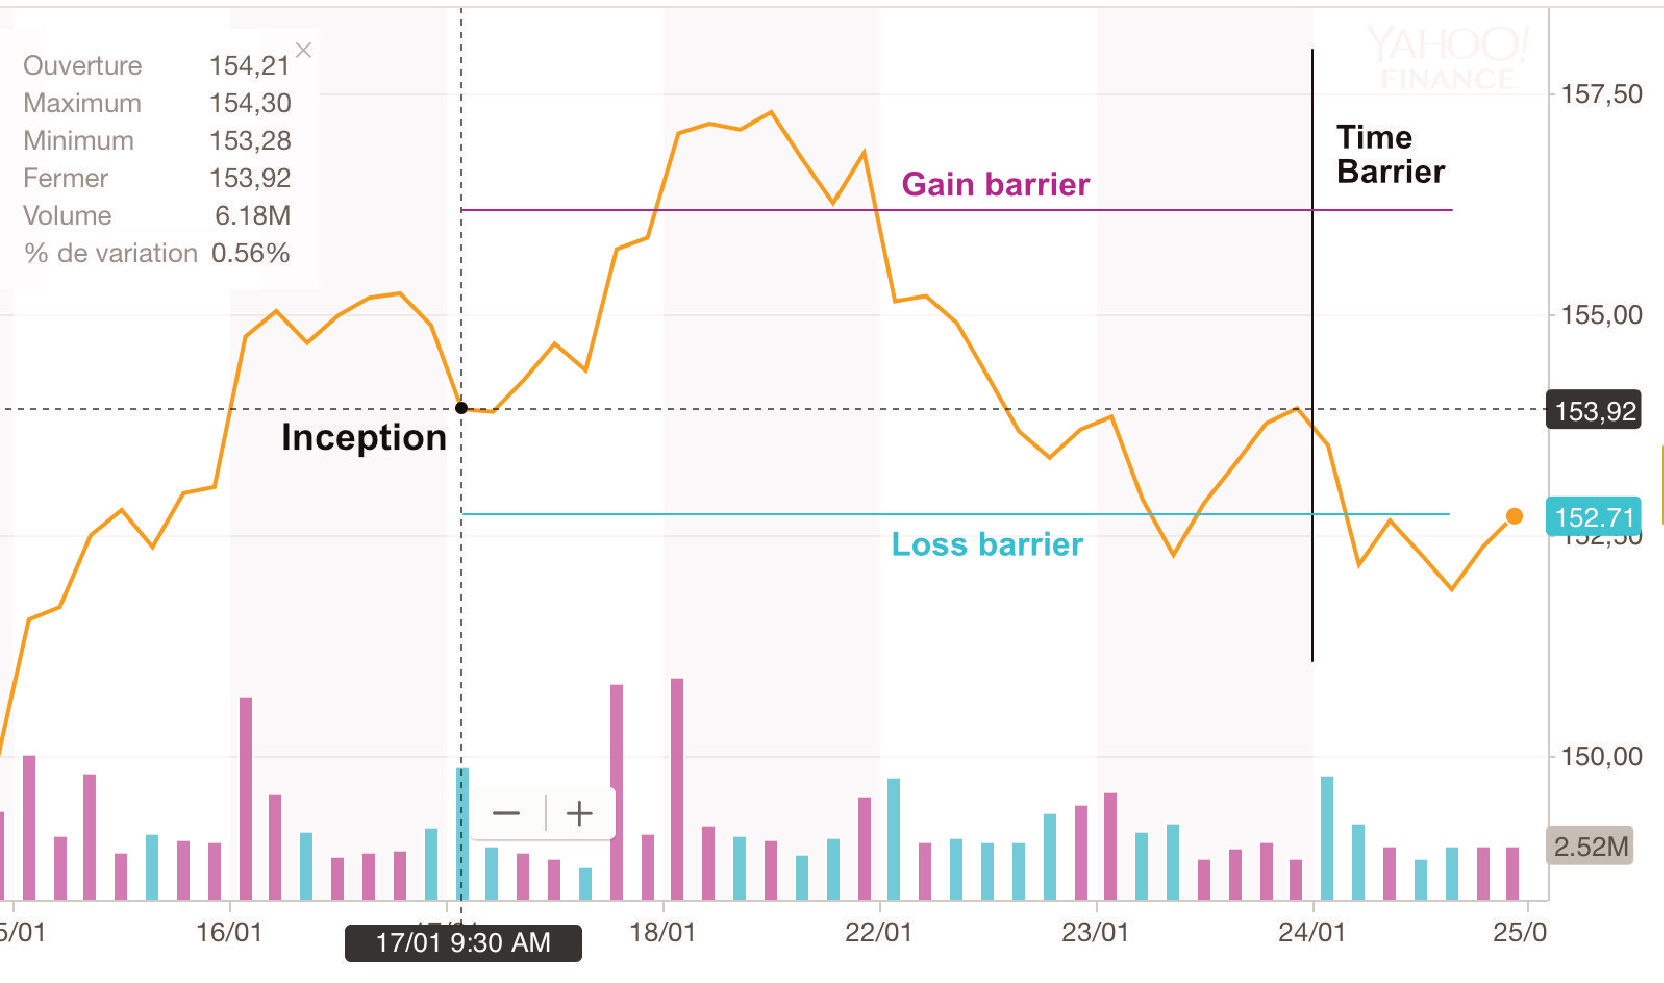
\includegraphics[width=0.7\linewidth]{files/triple_bar-d70a00c25f3a7a808961ace7962b05bc.pdf}
\caption[]{The triple barrier labelling method.}
\label{fig-triple_barrier}
\end{figure}

\paragraph{Filtering the sample}

{\textbackslash}index\{filtering training data\}
One of the main challenges in Machine Learning is to extract as much \textbf{signal} as possible. By signal, we mean patterns that will hold out-of-sample. Intuitively, it may seem reasonable to think that the more data we gather, the more signal we can extract. This is in fact false in all generality because more data also means more noise. Surprisingly, filtering the training samples can improve performance. This idea was for example implemented successfully in \cite{fu2018machine}, \cite{guida2019big} and \cite{guida2018machine}.

In \cite{coqueret2019training}, we investigate why smaller samples may lead to superior out-of-sample accuracy for a particular type of ML algorithm: decision trees (see Chapter \href{/chap-07-trees}{Tree-based methods}). We focus on a particular kind of filter: we exclude the labels (e.g., returns) that are not extreme and retain the 20\% values that are the smallest and the 20\% that are the largest (the bulk of the distribution is removed). In doing so, we alter the structure of trees in two ways:

\begin{itemize}
\item when the splitting points are altered, they are always closer to the center of the distribution of the splitting variable (i.e., the resulting clusters are more balanced and possibly more robust);
\item the choice of splitting variables is (sometimes) pushed towards the features that have a monotonic impact on the label.\newline
These two properties are desirable. The first reduces the risk of fitting to small groups of instances that may be spurious. The second gives more importance to features that appear globally more relevant in explaining the returns. However, the filtering must not be too intense. If, instead of retaining 20\% of each tail of the predictor, we keep just 10\%, then the loss in signal becomes too severe and the performance deteriorates.
\end{itemize}

\paragraph{Return horizons}\label{horizons}

This subsection deals with one of the least debated issues in factor-based machine learning models: horizons. Several horizons come into play during the whole ML-driven allocation workflow: the \textbf{horizon of the label}, the \textbf{estimation window} (chronological depth of the training samples) and the \textbf{holding periods}. One early reference that looks at these aspects is the founding academic paper on momentum by \cite{jegadeesh1993returns}. The authors compute the profitability of portfolios based on the returns over the past $J=3, 6, 9, 12$ months. Four holding periods are tested: $K=3,6,9,12$ months. They report: ``\textit{The most successful zero-cost (long-short) strategy selects stocks based on their returns over the previous 12 months and then holds the portfolio for 3 months}.'' While there is no machine learning whatsoever in this contribution, it is possible that their conclusion that horizons matter may also hold for more sophisticated methods. This topic is in fact much discussed, as is shown by the continuing debate on the impact of horizons in momentum profitability (see, e.g., \cite{novy2012momentum}, \cite{gong2015momentum} and \cite{goyal2015momentum}).

This debate should also be considered when working with ML algorithms (see for instance \cite{geertsema2020cross}). The issues of estimation windows and holding periods are mentioned later in the book, in Chapter \href{/chap-15-portfolio-backtesting}{Portfolio backtesting}. Naturally, in the present chapter, the horizon of the label is the important ingredient. Heuristically, there are four possible combinations if we consider only one feature for simplicity:

\begin{enumerate}
\item oscillating label and feature;
\item oscillating label, smooth feature (highly autocorrelated);
\item smooth label, oscillating feature;
\item smooth label and feature.
\end{enumerate}

Of all of these options, the last one is probably preferable because it is more robust, all things being equal.This is of course not the case for inference relying on linear models. Memory generates many problems and complicates the study of estimators. We refer to \cite{hjalmarsson2011new} and \cite{xu2020testing} for theoretical and empirical results on this matter. By \textit{all things being equal}, we mean that in each case, a model is capable of extracting some relevant pattern. A pattern that holds between two slowly moving series is more likely to persist in time. Thus, since features are often highly autocorrelated (cf Figure @ref(fig:histcorr)), combining them with smooth labels is probably a good idea. To illustrate how critical this point is, we will purposefully use 1-month returns in most of the examples of the book and show that the corresponding results are often disappointing. These returns are very weakly autocorrelated while 6-month or 12-month returns are much more persistent and are better choices for labels.

Theoretically, it is possible to understand why that may be the case. For simplicity, let us assume a single feature $x$ that explains returns $r$: $r_{t+1}=f(x_t)+e_{t+1}$. If $x_t$ is highly autocorrelated and the noise embeded in $e_{t+1}$ is not too large, then the two-period ahead return $(1+r_{t+1})(1+r_{t+2}) -1$ may carry more signal than $r_{t+1}$ because the relationship with $x_t$ has diffused and compounded through time. Consequently, it may also be beneficial to embed memory considerations directly into the modelling function, as is done for instance in \cite{dixon2020industrial}. We discuss some practicalities related to autocorrelations in the next section.

\subsubsection{Handling persistence}\label{pers}

{\textbackslash}index\{persistence\}
While we have separated the steps of feature engineering and labelling in two different subsections, it is probably wiser to consider them jointly. One important property of the dataset processed by the ML algorithm should be the consistency of persistence between features and labels. Intuitively, the autocorrelation patterns between the label $y_{t,n}$ (future performance) and the features $x_{t,n}^{(k)}$ should not be too distant.

One problematic example is when the dataset is sampled at the monthly frequency (not unusual in the money management industry) with the labels being monthly returns and the features being risk-based or fundamental attributes. In this case, the label is very weakly autocorrelated, while the features are often highly autocorrelated. In this situation, most sophisticated forecasting tools will arbitrage between features which will probably result in a lot of noise. In linear predictive models, this configuration is known to generate bias in estimates (see the study of \cite{stambaugh1999predictive} and the review by \cite{gonzalo2018predictive}).

Among other more technical options, there are two simple solutions when facing this issue: either introduce autocorrelation into the label, or remove it from the features. Again, the first option is not advised for statistical inference on linear models. Both are rather easy econometrically:

\begin{itemize}
\item to increase the autocorrelation of the label, compute performance over longer time ranges. For instance, when working with monthly data, considering annual or biennial returns will do the trick. {\textbackslash}index\{autocorrelation\}
\item to get rid of autocorrelation, the shortest route is to resort to differences/variations: $\Delta x_{t,n}^{(k)}=x_{t,n}^{(k)} -x_{t -1,n}^{(k)}$. One advantage of this procedure is that it makes sense, economically: variations in features may be better drivers of performance, compared to raw levels.
\end{itemize}

A mix between persistent and oscillating variables in the feature space is of course possible, as long as it is driven by economic motivations.

\subsubsection{Extensions}

\paragraph{Transforming features}

{\textbackslash}index\{feature transformation\}
The feature space can easily be augmented through simple operations. One of them is lagging, that is, considering older values of features and assuming some memory effect for their impact on the label. This is naturally useful mostly if the features are oscillating (adding a layer of memory on persistent features can be somewhat redundant). New variables are defined by $\breve{x}_{t,n}^{(k)}=x_{t -1,n}^{(k)}$.

In some cases (e.g., insufficient number of features), it is possible to consider ratios or products between features. Accounting ratios like price-to-book, book-to-market, debt-to-equity are examples of functions of raw features that make sense. The gains brought by a larger spectrum of features are not obvious. The risk of overfitting increases, just like in a simple linear regression adding variables mechanically increases the $R^2$. The choices must make sense, economically.

Another way to increase the feature space (mentioned above) is to consider variations. Variations in sentiment, variations in book-to-market ratio, etc., can be relevant predictors because sometimes, the change is more important than the level. In this case, a new predictor is $\breve{x}_{t,n}^{(k)}=x_{t,n}^{(k)} -x_{t -1,n}^{(k)}$.

\paragraph{Macro-economic variables}\label{sec_macrovar}

{\textbackslash}index\{macro-economic conditioning\}
Finally, we discuss a very important topic. The data should never be separated from the context it comes from (its environment). In classical financial terms, this means that a particular model is likely to depend on the overarching situation which is often proxied by macro-economic indicators. One way to take this into account at the data level is simply to multiply the feature by an exogenous indicator $z_{t}$ and in this case, the new predictor is
\begin{equation}
(\#eq:macrocond)
\breve{x}_{t,n}^{(k)}=z_t \times x_{t,n}^{(k)}
\end{equation}
This technique is used by \cite{gu2018empirical} who use 8 economic indicators (plus the original predictors ($z_t=1$)). This increases the feature space ninefold.

Another route that integrates shifting economic environments is conditional engineering. Suppose that labels are coded via formula \ref{catlabel}. The thresholds can be made dependent on some exogenous variable. In times of turbulence, it might be a good idea to increase both $r_+$ (buy threshold) and $r_ -$ (sell threshold) so that the labels become more conservative: it takes a higher return to make it to the \textit{buy} category, while short positions are favored. One such example of dynamic thresholding could be

\begin{equation}
(\#eq:condvix)
r_{t,\pm}=r_{\pm} \times e^{\pm\delta(\text{VIX}_t-\bar{\text{VIX}})},
\end{equation}

where $\text{VIX}_t$ is the time-$t$ value of the VIX, while $\bar{\text{VIX}}$ is some average or median value. When the VIX is above its average and risk seems to be increasing, the thresholds also increase. The parameter $\delta$ tunes the magnitude of the correction. In the above example, we assume $r_ -<0<r_+$.

\paragraph{Active learning}

{\textbackslash}index\{active learning\}

We end this section with the notion of active learning. To the best of our knowledge, it is not widely used in quantitative investment, but the underlying concept is enlightening, hence we dedicate a few paragraphs to this notion for the sake of completeness.

In general supervised learning, there is sometimes an asymmetry in the ability to gather features versus labels. For instance, it is free to have access to images, but the labelling of the content of the image (e.g., ``a dog'', ``a truck'', ``a pizza'', etc.) is costly because it requires human annotation. In formal terms, $\textbf{X}$ is cheap but the corresponding $\textbf{y}$ is expensive.

As is often the case when facing cost constraints, an evident solution is greed. Ahead of the usual learning process, a filter (often called \textit{query}) is used to decide which data to label and train on (possibly in relationship with the ML algorithm). The labelling is performed by a so-called \textit{oracle} (which/who knows the truth), usually human. This technique that focuses on the most informative instances is referred to as \textbf{active learning}. We refer to the surveys of \cite{settles2009active} and \cite{settles2012active} for a detailed account of this field (which we briefly summarize below). The term \textbf{active} comes from the fact that the learner does not passively accept data samples but actively participates in the choices of items it learns from.

One major dichotomy in active learning pertains to the data source $\textbf{X}$ on which the query is based. One obvious case is when the original sample $\textbf{X}$ is very large and not labelled and the learner asks for particular instances within this sample to be labelled. The second case is when the learner has the ability to simulate/generate its own values $\textbf{x}_i$. This can sometimes be problematic if the oracle does not recognize the data that is generated by the machine. For instance, if the purpose is to label images of characters and numbers, the learner may generate shapes that do not correspond to any letter or digit: the oracle cannot label it.

In active learning, one key question is, how does the learner choose the instances to be labelled? Heuristically, the answer is by picking those observations that maximize learning efficiency. In binary classification, a simple criterion is the probability of belonging to one particular class. If this probability is far from 0.5, then the algorithm will have no difficulty of picking one class (even though it can be wrong). The interesting case is when the probability is close to 0.5: the machine may hesitate for this particular instance. Thus, having the oracle label it is useful in this case because it helps the learner in a configuration in which it is undecided.

Other methods seek to estimate the fit that can be obtained when including particular (new) instances in the training set, and then to optimize this fit. Recalling Section 3.1 in \cite{geman1992neural} on the variance-bias tradeoff, we have, for a training dataset $D$ and one instance $x$ (we omit the bold font for simplicity),
\begin{equation}
\mathbb{E}\left[\left.(y-\hat{f}(x;D))^2\right|\{D,x\}\right]=\mathbb{E}\left[\left.\underbrace{(y-\mathbb{E}[y|x])^2}_{\text{indep. from }D\text{ and }\hat{f}} \right|\{D,x\} \right]+(\hat{f}(x;D)-\mathbb{E}[y|x])^2,
\end{equation}
where the notation $f(x;D)$ is used to highlight the dependence between the model $\hat{f}$ and the dataset $D$: the model has been trained on $D$. The first term is irreducible, as it does not depend on $\hat{f}$. Thus, only the second term is of interest. If we take the average of this quantity, taken over all possible values of $D$:
\begin{equation}
\mathbb{E}_D\left[(\hat{f}(x;D)-\mathbb{E}[y|x])^2  \right]=\underbrace{\left(\mathbb{E}_D\left[\hat{f}(x;D)-\mathbb{E}[y|x]\right]\right)^2}_{\text{squared bias}} \ + \ \underbrace{\mathbb{E}_D\left[(\hat{f}(x,D)-\mathbb{E}_D[\hat{f}(x;D)])^2\right]}_{\text{variance}}
\end{equation}
If this expression is not too complicated to compute, the learner can query the $x$ that minimizes the tradeoff.{\textbackslash}index\{variance-bias tradeoff\} Thus, on average, this new instance will be the one that yields the best learning angle (as measured by the $L^2$ error). Beyond this approach (which is limited because it requires the oracle to label a possibly irrelevant instance), many other criteria exist for querying and we refer to section 3 from \cite{settles2009active} for an exhaustive list.

One final question: is active learning applicable to factor investing? One straightfoward answer is that data cannot be annotated by human intervention. Thus, the learners cannot simulate their own instances and ask for corresponding labels. One possible option is to provide the learner with $\textbf{X}$ but not $\textbf{y}$ and keep only a queried subset of observations with the corresponding labels. In spirit, this is close to what is done in \cite{coqueret2019training} except that the query is not performed by a machine but by the human user. Indeed, it is shown in this paper that not all observations carry the same amount of signal. Instances with `average' label values seem to be on average less informative compared to those with extreme label values.

\subsubsection{Additional code and results}

\paragraph{Impact of rescaling: graphical representation}

We start with a simple illustration of the different scaling methods. We generate an arbitrary series and then rescale it. The series is not random so that each time the code chunk is executed, the output remains the same.

\begin{verbatim}
# Generate an arbitrary series
Length = 100
x = np.exp(np.sin(np.arange(1, Length + 1)))

# Create DataFrame with original data
data = pd.DataFrame({
    'index': np.arange(1, Length + 1),
    'x': x
})

# Plot original data
fig, ax = plt.subplots(figsize=(10, 4))
ax.bar(data['index'], data['x'], width=1, edgecolor='white')
ax.set_xlabel('Index')
ax.set_ylabel('x')
ax.set_title('Original Data')
plt.tight_layout()
plt.show()
\end{verbatim}

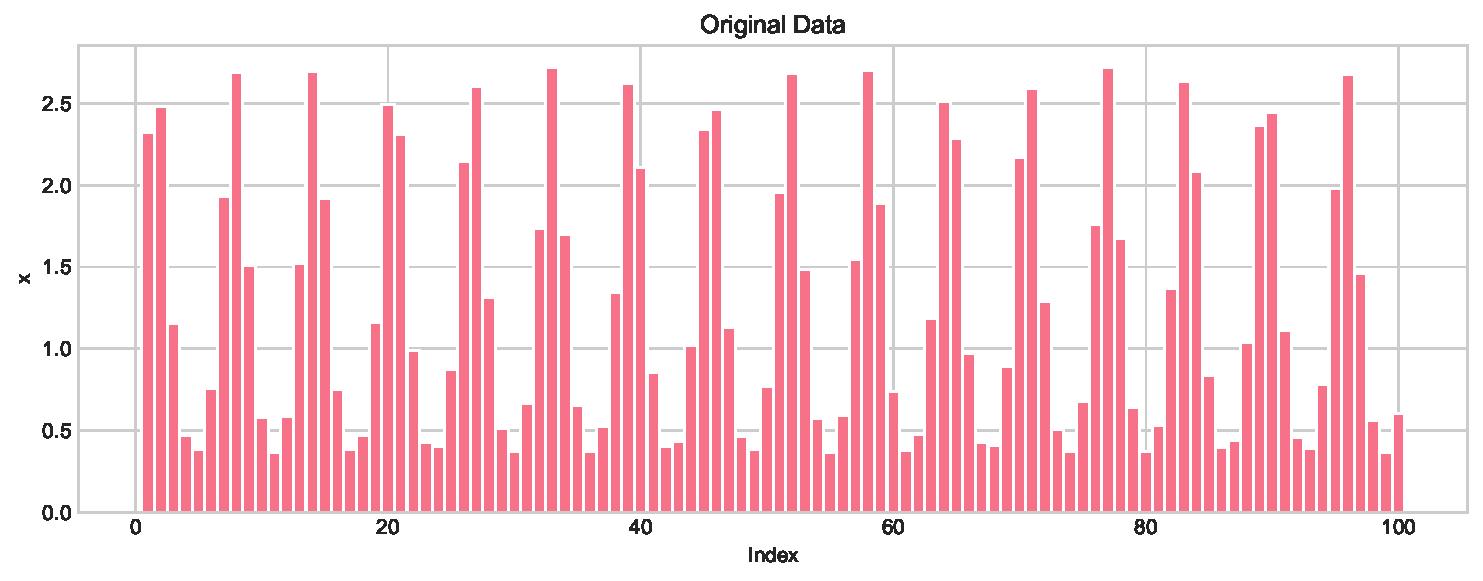
\includegraphics[width=0.7\linewidth]{files/4d85b92fbc83150f925401eab4742c67.pdf}

We define and plot the scaled variables below.

\begin{verbatim}
# Compute scaled versions
data_norm = pd.DataFrame({
    'index': np.arange(1, Length + 1),
    'standard': standardize(x),
    'norm_0_1': norm_0_1(x),
    'unif': norm_unif(x)
})

# Melt to long format for plotting
data_norm_long = data_norm.melt(
    id_vars='index',
    var_name='Type',
    value_name='value'
)

# Plot scaled variables
fig, axes = plt.subplots(3, 1, figsize=(10, 8), sharex=True)

for ax, (name, group) in zip(axes, data_norm_long.groupby('Type')):
    ax.bar(group['index'], group['value'], width=1, edgecolor='white')
    ax.set_ylabel(name)

axes[-1].set_xlabel('Index')
plt.suptitle('Scaled Variables Comparison')
plt.tight_layout()
plt.show()
\end{verbatim}

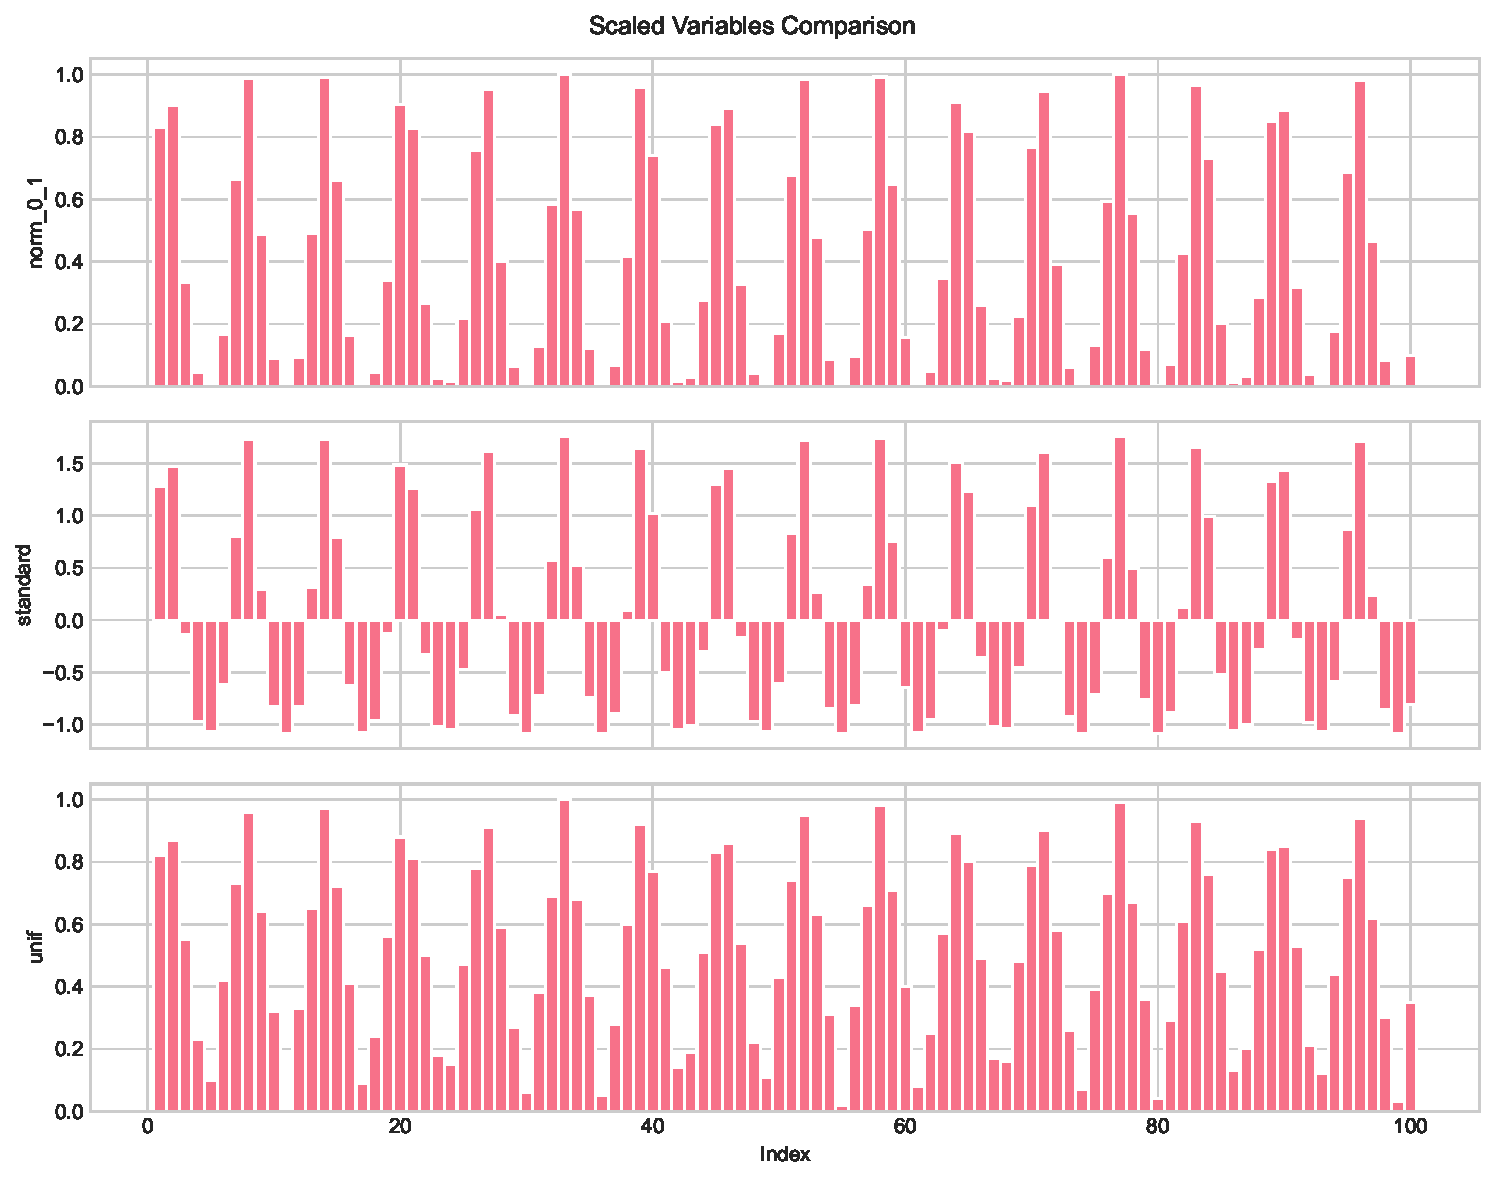
\includegraphics[width=0.7\linewidth]{files/5f75e2557a5913126d33577b88948f3e.pdf}

Finally, we look at the histogram of the newly created variables.

\begin{verbatim}
# Histogram of scaled variables
fig, ax = plt.subplots(figsize=(10, 5))

for scaling_type in ['standard', 'norm_0_1', 'unif']:
    ax.hist(data_norm[scaling_type], bins=20, alpha=0.5, label=scaling_type)

ax.set_xlabel('Value')
ax.set_ylabel('Frequency')
ax.legend(title='Type')
ax.set_title('Distribution of Scaled Variables')
plt.tight_layout()
plt.show()
\end{verbatim}

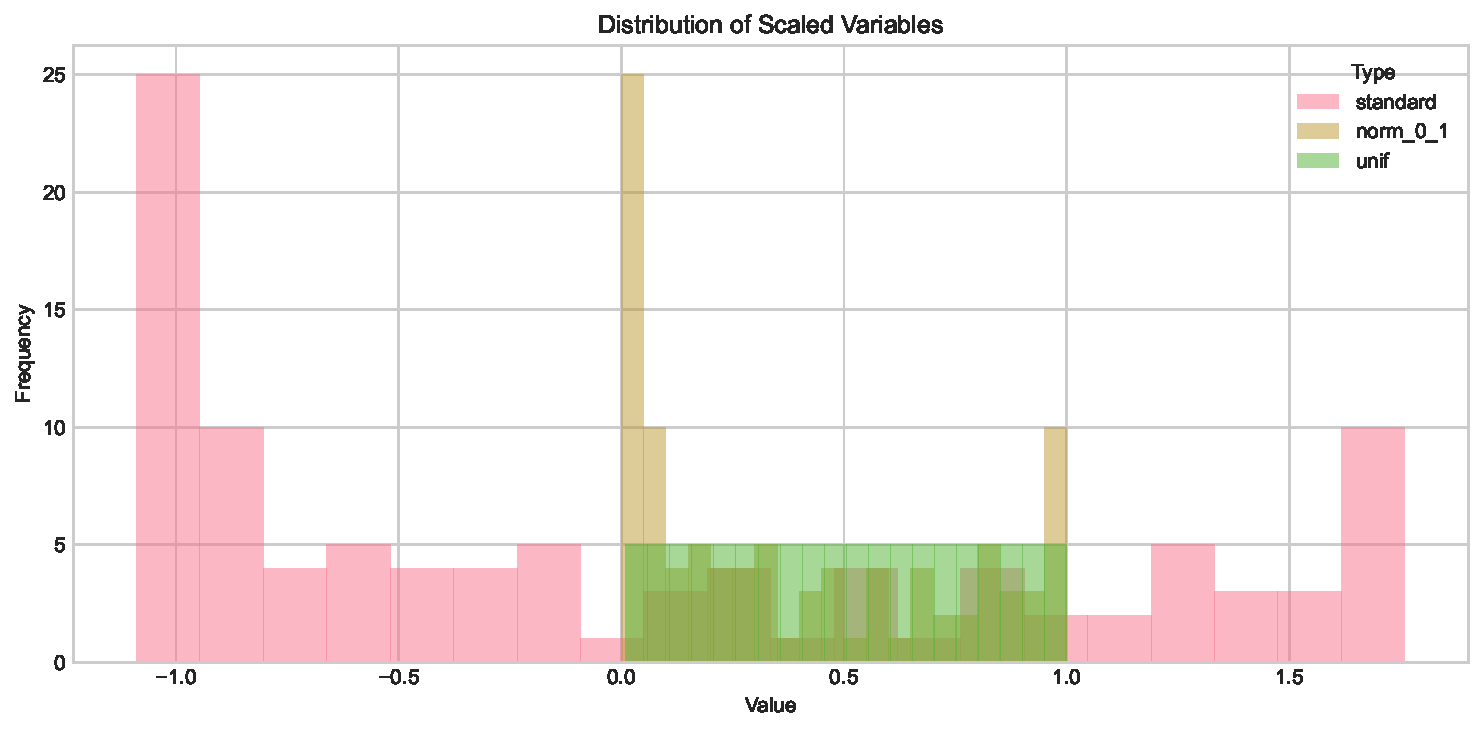
\includegraphics[width=0.7\linewidth]{files/65b3e53e2f0475f1231ba188b8f10828.pdf}

With respect to shape, the yellow-ish and red distributions are close to the original one. It is only the support that changes: the min/max rescaling ensures all values lie in the $[0,1]$ interval. In both cases, the smallest values (on the left) display a spike in distribution. By construction, this spike disappears under the uniformization: the points are evenly distributed over the unit interval (green distribution).

\paragraph{Impact of rescaling: toy example}

To illustrate the impact of choosing one particular rescaling method,\footnote{For a more thorough technical discussion on the impact of feature engineering, we refer to \cite{galili2016splitting}.} we build a simple dataset, comprising 3 firms and 3 dates.

\begin{verbatim}
# Create toy dataset
firm = [1, 1, 1, 2, 2, 2, 3, 3, 3]
date = [1, 2, 3, 1, 2, 3, 1, 2, 3]
cap = [10, 50, 100, 15, 10, 15, 200, 120, 80]
returns = [0.06, 0.01, -0.06, -0.03, 0.00, 0.02, -0.04, -0.02, 0.00]

data_toy = pd.DataFrame({
    'firm': firm,
    'date': date,
    'cap': cap,
    'return': returns
})

# Apply scaling within each date
data_toy['cap_0_1'] = data_toy.groupby('date')['cap'].transform(norm_0_1)
data_toy['cap_u'] = data_toy.groupby('date')['cap'].transform(norm_unif)

data_toy.round(3)
\end{verbatim}

\bigskip\noindent
\begin{tabular}{p{\dimexpr 0.143\linewidth-2\tabcolsep}p{\dimexpr 0.143\linewidth-2\tabcolsep}p{\dimexpr 0.143\linewidth-2\tabcolsep}p{\dimexpr 0.143\linewidth-2\tabcolsep}p{\dimexpr 0.143\linewidth-2\tabcolsep}p{\dimexpr 0.143\linewidth-2\tabcolsep}p{\dimexpr 0.143\linewidth-2\tabcolsep}}
\toprule
 & firm & date & cap & return & cap\_0\_1 & cap\_u \\
\hline
0 & 1 & 1 & 10 & 0.06 & 0.000 & 0.333 \\
\hline
1 & 1 & 2 & 50 & 0.01 & 0.364 & 0.667 \\
\hline
2 & 1 & 3 & 100 & -0.06 & 1.000 & 1.000 \\
\hline
3 & 2 & 1 & 15 & -0.03 & 0.026 & 0.667 \\
\hline
4 & 2 & 2 & 10 & 0.00 & 0.000 & 0.333 \\
\hline
5 & 2 & 3 & 15 & 0.02 & 0.000 & 0.333 \\
\hline
6 & 3 & 1 & 200 & -0.04 & 1.000 & 1.000 \\
\hline
7 & 3 & 2 & 120 & -0.02 & 1.000 & 1.000 \\
\hline
8 & 3 & 3 & 80 & 0.00 & 0.765 & 0.667 \\
\hline
\bottomrule
\end{tabular}

\bigskip

Let's briefly comment on this synthetic data. We assume that dates are ordered chronologically and far away: each date stands for a year or the beginning of a decade, but the (forward) returns are computed on a monthly basis. The first firm is hugely successful and multiplies its cap ten times over the periods. The second firm remains stable cap-wise, while the third one plummets. If we look at `local' future returns, they are strongly negatively related to size for the first and third firms. For the second one, there is no clear pattern.

\begin{verbatim}
import statsmodels.api as sm

# Regression with min-max rescaled variable
X1 = sm.add_constant(data_toy['cap_0_1'])
model1 = sm.OLS(data_toy['return'], X1).fit()
print("Regression output with min-max rescaling:")
print(model1.summary().tables[1])
print()
\end{verbatim}

\begin{verbatim}
Regression output with min-max rescaling:
==============================================================================
                 coef    std err          t      P>|t|      [0.025      0.975]
------------------------------------------------------------------------------
const          0.0163      0.014      1.185      0.275      -0.016       0.049
cap_0_1       -0.0497      0.021     -2.326      0.053      -0.100       0.001
==============================================================================
\end{verbatim}

\begin{verbatim}
# Regression with uniformized variable
X2 = sm.add_constant(data_toy['cap_u'])
model2 = sm.OLS(data_toy['return'], X2).fit()
print("Regression output with uniformization:")
print(model2.summary().tables[1])
\end{verbatim}

\begin{verbatim}
Regression output with uniformization:
==============================================================================
                 coef    std err          t      P>|t|      [0.025      0.975]
------------------------------------------------------------------------------
const          0.0600      0.020      3.028      0.019       0.013       0.107
cap_u         -0.1000      0.028     -3.634      0.008      -0.165      -0.035
==============================================================================
\end{verbatim}

Note the difference in p-values between the two scaling methods. The standard deviation of \texttt{cap\_0\_1} and \texttt{cap\_u} are:

\begin{itemize}
\item \texttt{cap\_0\_1}: 0.47
\item \texttt{cap\_u}: 0.29
\end{itemize}

Uniformized variables have reduced dispersion, which can help but is also a double-edged sword.

\begin{verbatim}
print(f"Standard deviation of cap_0_1: {data_toy['cap_0_1'].std():.2f}")
print(f"Standard deviation of cap_u: {data_toy['cap_u'].std():.2f}")
\end{verbatim}

\begin{verbatim}
Standard deviation of cap_0_1: 0.47
Standard deviation of cap_u: 0.29
\end{verbatim}

\subsubsection{Labelling}

\paragraph{Simple labels}

Usual labels in factor investing:

\begin{itemize}
\item Raw asset returns
\item Future relative returns (versus some benchmark)
\item Probability of positive return
\item Probability of outperforming a benchmark
\item Binary: YES (outperforming) vs NO (underperforming)
\item Risk-adjusted versions: Sharpe ratios, information ratios, etc.
\end{itemize}

\paragraph{Categorical labels}

\begin{equation}
y_{t,i}=\begin{cases}
-1 & \text{if } \hat{r}_{t,i} < r_- \\
0 & \text{if } \hat{r}_{t,i} \in [r_-, r_+] \\
+1 & \text{if } \hat{r}_{t,i} > r_+
\end{cases}
\end{equation}

\begin{verbatim}
def create_categorical_label(returns, r_minus, r_plus):
    """
    Create categorical labels based on return thresholds.
    """
    labels = pd.Series(0, index=returns.index)
    labels[returns < r_minus] = -1
    labels[returns > r_plus] = 1
    return labels

def one_hot_encode(labels):
    """
    One-hot encode categorical labels.
    """
    return pd.get_dummies(labels, prefix='label')
\end{verbatim}

\paragraph{Dynamic thresholds with VIX conditioning}

\begin{equation}
r_{t,\pm} = r_{\pm} \times e^{\pm\delta(\text{VIX}_t - \bar{\text{VIX}})}
\end{equation}

\begin{verbatim}
def dynamic_thresholds(vix_t, vix_mean, r_minus, r_plus, delta=0.1):
    """
    Compute dynamic thresholds based on VIX conditioning.
    """
    adjustment = np.exp(delta * (vix_t - vix_mean))
    return r_minus * adjustment, r_plus * adjustment
\end{verbatim}

\subsubsection{Extensions}

\paragraph{Transforming features}

\begin{itemize}
\item \textbf{Lagging}: $\breve{x}_{t,n}^{(k)} = x_{t -1,n}^{(k)}$
\item \textbf{Variations}: $\breve{x}_{t,n}^{(k)} = x_{t,n}^{(k)} - x_{t -1,n}^{(k)}$
\end{itemize}

\paragraph{Macro-economic conditioning}

\begin{equation}
\breve{x}_{t,n}^{(k)} = z_t \times x_{t,n}^{(k)}
\end{equation}

\begin{verbatim}
def add_lagged_features(df, features, id_col='fsym_id', lag=1):
    """
    Add lagged versions of features.
    """
    df_lagged = df.copy()
    for feature in features:
        df_lagged[f'{feature}_lag{lag}'] = df_lagged.groupby(id_col)[feature].shift(lag)
    return df_lagged

def add_feature_variations(df, features, id_col='fsym_id'):
    """
    Add first-difference (variation) versions of features.
    """
    df_diff = df.copy()
    for feature in features:
        df_diff[f'{feature}_diff'] = df_diff.groupby(id_col)[feature].diff()
    return df_diff

def add_macro_conditioned_features(df, features, macro_indicator):
    """
    Add macro-conditioned features: feature * macro_indicator.
    
    Parameters:
    -----------
    df : pd.DataFrame
        Dataset
    features : list
        List of feature column names
    macro_indicator : pd.Series
        Time series of macro indicator (indexed by date)
    """
    df_conditioned = df.copy()
    for feature in features:
        df_conditioned[f'{feature}_macro'] = df_conditioned[feature] * macro_indicator
    return df_conditioned
\end{verbatim}

\subsubsection{Coding exercises}

\begin{enumerate}
\item The Federal Reserve of Saint Louis (\href{https://fred.stlouisfed.org}{https://fred.stlouisfed.org}) hosts thousands of time series of economic indicators that can serve as conditioning variables. Pick one and apply the macro-conditioning formula to expand the number of predictors.
\item Create a new categorical label based on the dynamic VIX threshold formula. The time series of the VIX can be retrieved from: \href{https://fred.stlouisfed.org/series/VIXCLS}{https://fred.stlouisfed.org/series/VIXCLS}
\item Plot the histogram of the R12M\_Usd variable. Identify the stock with highest value for this variable and determine if the value can be correct or not.
\end{enumerate}

\section{Common supervised algorithms}

\subsection{Penalized regressions and sparse hedging for minimum variance portfolios}

% # (PART) Common supervised algorithms {-}

{\textbackslash}index\{penalized regression\}

In this chapter, we introduce the widespread concept of regularization for linear models. There are in fact several possible applications for these models. The first one is straightforward: resort to penalizations to improve the robustness of factor-based predictive regressions. The outcome can then be used to fuel an allocation scheme. For instance, \cite{han2018firm} and \cite{rapach2019time} use penalized regressions to improve stock return prediction when combining forecasts that emanate from individual characteristics.

Similar ideas can be developed for macroeconomic predictions for instance, as in \cite{uematsu2019high}.
The second application stems from a less known result which originates from \cite{stevens1998inverse}. It links the weights of optimal mean-variance portfolios to particular cross-sectional regressions. The idea is then different and the purpose is to improve the quality of mean-variance driven portfolio weights. We present the two approaches below after an introduction on regularization techniques for linear models.

Other examples of financial applications of penalization can be found in \cite{d2011identifying}, \cite{ban2016machine} and \cite{kremer2019sparse}. In any case, the idea is the same as in the seminal paper \cite{tibshirani1996regression}: standard (unconstrained) optimization programs may lead to noisy estimates, thus adding a structuring constraint helps remove some noise (at the cost of a possible bias). For instance, \cite{kremer2019sparse} use this concept to build more robust mean-variance \citep{markowitz1952portfolio} portfolios and \cite{freyberger2020dissecting} use it to single out the characteristics that \textit{really} help explain the cross-section of equity returns.

\subsubsection{Penalized regressions}

{\textbackslash}index\{penalized regression\}

\paragraph{Simple regressions}\label{penreg}

{\textbackslash}index\{simple regression\} {\textbackslash}index\{regression\}
The ideas behind linear models are at least two centuries old (\cite{legendre1805nouvelles} is an early reference on least squares optimization). Given a matrix of predictors $\textbf{X}$, we seek to decompose the output vector $\textbf{y}$ as a linear function of the columns of $\textbf{X}$ (written $\textbf{X}\boldsymbol{\beta}$) plus an error term $\boldsymbol{\epsilon}$: $\textbf{y}=\textbf{X}\boldsymbol{\beta}+\boldsymbol{\epsilon}$.

The best choice of $\boldsymbol{\beta}$ is naturally the one that minimizes the error. For analytical tractability, it is the sum of squared errors that is minimized: $L=\boldsymbol{\epsilon}'\boldsymbol{\epsilon}=\sum_{i=1}^I\epsilon_i^2$. The loss $L$ is called the sum of squared residuals (SSR). In order to find the optimal $\boldsymbol{\beta}$, it is imperative to differentiate this loss $L$ with respect to $\boldsymbol{\beta}$ because the first order condition requires that the gradient be equal to zero:
\begin{align*}
\nabla_{\boldsymbol{\beta}} L&=\frac{\partial}{\partial \boldsymbol{\beta}}(\textbf{y}-\textbf{X}\boldsymbol{\beta})'(\textbf{y}-\textbf{X}\boldsymbol{\beta})=\frac{\partial}{\partial \boldsymbol{\beta}}\boldsymbol{\beta}'\textbf{X}'\textbf{X}\boldsymbol{\beta}-2\textbf{y}'\textbf{X}\boldsymbol{\beta} \\
&=2\textbf{X}'\textbf{X}\boldsymbol{\beta}  -2\textbf{X}'\textbf{y}
\end{align*}
so that the first order condition $\nabla_{\boldsymbol{\beta}}=\textbf{0}$ is satisfied if

\begin{equation}
\label{regbeta}
\boldsymbol{\beta}^*=(\textbf{X}'\textbf{X})^{-1}\textbf{X}'\textbf{y},
\end{equation}

which is known as the standard \textbf{ordinary least squares} (OLS){\textbackslash}index\{ordinary least squares\} solution of the linear model. If the matrix $\textbf{X}$ has dimensions $I \times K$, then the $\textbf{X}'\textbf{X}$ can only be inverted if the number of rows $I$ is strictly superior to the number of columns $K$. In some cases, that may not hold; there are more predictors than instances and there is no unique value of $\boldsymbol{\beta}$ that minimizes the loss. If $\textbf{X}'\textbf{X}$ is nonsingular (or positive definite), then the second order condition ensures that $\boldsymbol{\beta}^*$ yields a global minimum for the loss $L$ (the second order derivative of $L$ with respect to $\boldsymbol{\beta}$, the Hessian matrix, is exactly $\textbf{X}'\textbf{X}$).

Up to now, we have made no distributional assumption on any of the above quantities. Standard assumptions are the following:

\begin{itemize}
\item $\mathbb{E}[\textbf{y}|\textbf{X}]=\textbf{X}\boldsymbol{\beta}$: \textbf{linear shape for the regression function};
\item $\mathbb{E}[\boldsymbol{\epsilon}|\textbf{X}]=\textbf{0}$: errors are \textbf{independent of predictors};
\item $\mathbb{E}[\boldsymbol{\epsilon}\boldsymbol{\epsilon}'| \textbf{X}]=\sigma^2\textbf{I}$: \textbf{homoscedasticity} - errors are uncorrelated and have identical variance;
\item the $\epsilon_i$ are normally distributed.
\end{itemize}

Under these hypotheses, it is possible to perform statistical tests related to the $\hat{\boldsymbol{\beta}}$ coefficients. We refer to chapters 2 to 4 in \cite{greene2018econometric} for a thorough treatment on linear models as well as to chapter 5 of the same book for details on the corresponding tests.

\paragraph{Forms of penalizations}

{\textbackslash}index\{penalized regression\}
Penalized regressions have been popularized since the seminal work of \cite{tibshirani1996regression}. The idea is to impose a constraint on the coefficients of the regression, namely that their total magnitude be restrained. In his original paper, \cite{tibshirani1996regression} proposes to estimate the following model (LASSO):{\textbackslash}index\{LASSO\}

\begin{equation}
\label{lasso1}
y_i = \sum_{j=1}^J \beta_jx_{i,j} + \epsilon_i, \quad i =1,\dots,I, \quad \text{s.t.} \quad \sum_{j=1}^J |\beta_j| < \delta,
\end{equation}

for some strictly positive constant $\delta$. Under least square minimization, this amounts to solve the Lagrangian formulation:

\begin{equation}
\label{lasso2}
\underset{\mathbf{\beta}}{\min} \, \left\{ \sum_{i=1}^I\left(y_i - \sum_{j=1}^J \beta_jx_{i,j} \right)^2+\lambda \sum_{j=1}^J |\beta_j| \right\},
\end{equation}

for some value $\lambda>0$ which naturally depends on $\delta$ (the lower the $\delta$, the higher the $\lambda$: the constraint is more binding). This specification seems close to the ridge regression ($L^2$ regularization), which is in fact anterior to the Lasso:{\textbackslash}index\{ridge regression\}

\begin{equation}
\label{ridge}
\underset{\mathbf{\beta}}{\min} \, \left\{ \sum_{i=1}^I\left(y_i - \sum_{j=1}^J\beta_jx_{i,j} \right)^2+\lambda \sum_{j=1}^J \beta_j^2 \right\},
\end{equation}

and which is equivalent to estimating the following model

\begin{equation}
\label{ridge6}
y_i = \sum_{j=1}^J \beta_jx_{i,j} + \epsilon_i, \quad i =1,\dots,I, \quad \text{s.t.} \quad \sum_{j=1}^J \beta_j^2 < \delta,
\end{equation}

but the outcome is in fact quite different, which justifies a separate treatment. Mechanically, as $\lambda$, the penalization intensity,{\textbackslash}index\{penalization intensity\} increases (or as $\delta$ in \ref{ridge6} \textit{decreases}), the coefficients of the ridge regression all slowly decrease in magnitude towards zero. In the case of the LASSO, the convergence is somewhat more brutal as some coefficients shrink to zero very quickly. For $\lambda$ sufficiently large, only one coefficient will remain nonzero, while in the ridge regression, the zero value is only reached asymptotically for all coefficients. We invite the interested read to have a look at the survey in \cite{hastie2020ridge} about all applications of ridge regressions in data science with links to other topics like cross-validation{\textbackslash}index\{cross-validation\} and dropout regularization{\textbackslash}index\{dropout\}, among others.{\textbackslash}index\{ridge regression\}

To depict the difference between the Lasso and the ridge regression, let us consider the case of $K=2$ predictors which is shown in Figure~\ref{fig-lassoridge}. The optimal unconstrained solution $\boldsymbol{\beta}^*$ is pictured in red in the middle of the space. The problem is naturally that it does not satisfy the imposed conditions. These constraints are shown in light grey: they take the shape of a square $|\beta_1|+|\beta_2| \le \delta$ in the case of the Lasso and a circle $\beta_1^2+\beta_2^2 \le \delta$ for the ridge regression. In order to satisfy these constraints, the optimization needs to look in the vicinity of $\boldsymbol{\beta}^*$ by allowing for larger error levels. These error levels are shown as orange ellipsoids in the figure. When the requirement on the error is loose enough, one ellipsoid touches the acceptable boundary (in grey) and this is where the constrained solution is located.

\begin{figure}[!htbp]
\centering
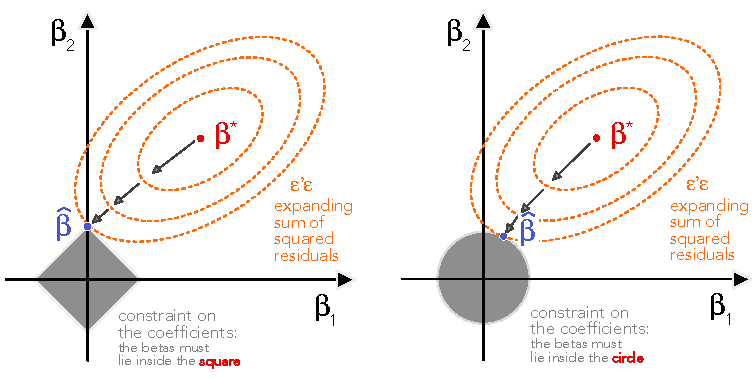
\includegraphics[width=0.7\linewidth]{files/lassoridge-e1f18e925b7de28412a81fdeeb5c4766.pdf}
\caption[]{Schematic view of Lasso (left) versus ridge (right) regressions.}
\label{fig-lassoridge}
\end{figure}

Both methods work when the number of exogenous variables surpasses that of observations, i.e., in the case where classical regressions are ill-defined. This is easy to see in the case of the ridge regression for which the OLS solution is simply
\begin{equation}
\hat{\boldsymbol{\beta}}=(\mathbf{X}'\mathbf{X}+\lambda \mathbf{I}_N)^{-1}\mathbf{X}'\mathbf{Y}.
\end{equation}
The additional term $\lambda \mathbf{I}_N$ compared to Equation \ref{regbeta} ensures that the inverse matrix is well-defined whenever $\lambda>0$. As $\lambda$ increases, the magnitudes of the $\hat{\beta}_i$ decrease, which explains why penalizations are sometimes referred to as \textbf{shrinkage} methods (the estimated coefficients see their values shrink). {\textbackslash}index\{ridge regression\}

\cite{zou2005regularization} propose to benefit from the best of both worlds when combining both penalizations in a convex manner (which they call the \textbf{elasticnet}):{\textbackslash}index\{elasticnet\}

\begin{equation}
\label{elasticnet}
y_i = \sum_{j=1}^J \beta_jx_{i,j} + \epsilon_i, \quad \text{s.t.} \quad \alpha \sum_{j=1}^J |\beta_j| +(1-\alpha)\sum_{j=1}^J \beta_j^2< \delta, \quad i =1,\dots,N,
\end{equation}

which is associated to the optimization program

\begin{equation}
\label{elastic}
\underset{\mathbf{\beta}}{\min} \, \left\{ \sum_{i=1}^I\left(y_i - \sum_{j=1}^J\beta_jx_{i,j} \right)^2+\lambda \left(\alpha\sum_{j=1}^J |\beta_j|+ (1-\alpha)\sum_{j=1}^J \beta_j^2\right) \right\}.
\end{equation}

The main advantage of the LASSO compared to the ridge regression is its selection capability. Indeed, given a very large number of variables (or predictors), the LASSO will progressively rule out those that are the least relevant. The elasticnet preserves this selection ability and \cite{zou2005regularization} argue that in some cases, it is even more effective than the LASSO. The parameter $\alpha \in [0,1]$ tunes the smoothness of convergence (of the coefficients) towards zero. The closer $\alpha$ is to zero, the smoother the convergence.

\paragraph{Illustrations}

We begin with simple illustrations of penalized regressions. We start with the LASSO. First, we estimate the coefficients. By default, the function chooses a large array of penalization values so that the results for different penalization intensities ($\lambda$) can be shown immediately.{\textbackslash}index\{penalized regression\}

\begin{verbatim}
from sklearn.linear_model import lasso_path, Ridge, ElasticNet
import pandas as pd
import numpy as np
import matplotlib.pyplot as plt
import seaborn as sns
from scipy import stats
from statsmodels.tsa.stattools import acf
import warnings
warnings.filterwarnings('ignore')
plt.style.use('seaborn-v0_8-whitegrid')
sns.set_palette("husl")

# Building the data & import functions
from data_build import generate_data
data_ml, features, features_short, returns, stock_ids, stock_ids_short = generate_data()
features_short =["Div_yld", "EPS", "size_avg_252d", "mom_252", "OCF_Growth_1Y", "PB", "vol_252"]
separation_date = "2017-01-15"

data_ml_clean = data_ml.dropna(subset=(features_short + ['R1M']))
y_penalized = data_ml_clean['R1M'].values
x_penalized = data_ml_clean[features_short].values

# Compute LASSO path (alpha=1 in sklearn corresponds to pure LASSO)
alphas_lasso, coefs_lasso, _ = lasso_path(x_penalized, y_penalized)  # Model: LASSO
\end{verbatim}

Once the coefficients are computed, they require some wrangling before plotting. Also, there are too many of them, so we only plot a subset of them.

\begin{figure}[!htbp]
\centering
\begin{verbatim}
n_features_to_plot = min(10, len(features_short)) 

plt.rcParams.update({'font.size': 14})
plt.figure(figsize=(10, 6))
for i in range(n_features_to_plot):
    plt.plot(alphas_lasso, coefs_lasso[i, :], label=features[i])

plt.xlabel('Lambda')
plt.ylabel('beta')
plt.xscale('log')
plt.gca().invert_xaxis()  # Higher lambda = more regularization
plt.tight_layout()
plt.legend(fontsize=12, loc='best', facecolor='white')
plt.show()
\end{verbatim}
\caption[]{LASSO coefficients. The dependent variable is the 1 month ahead return

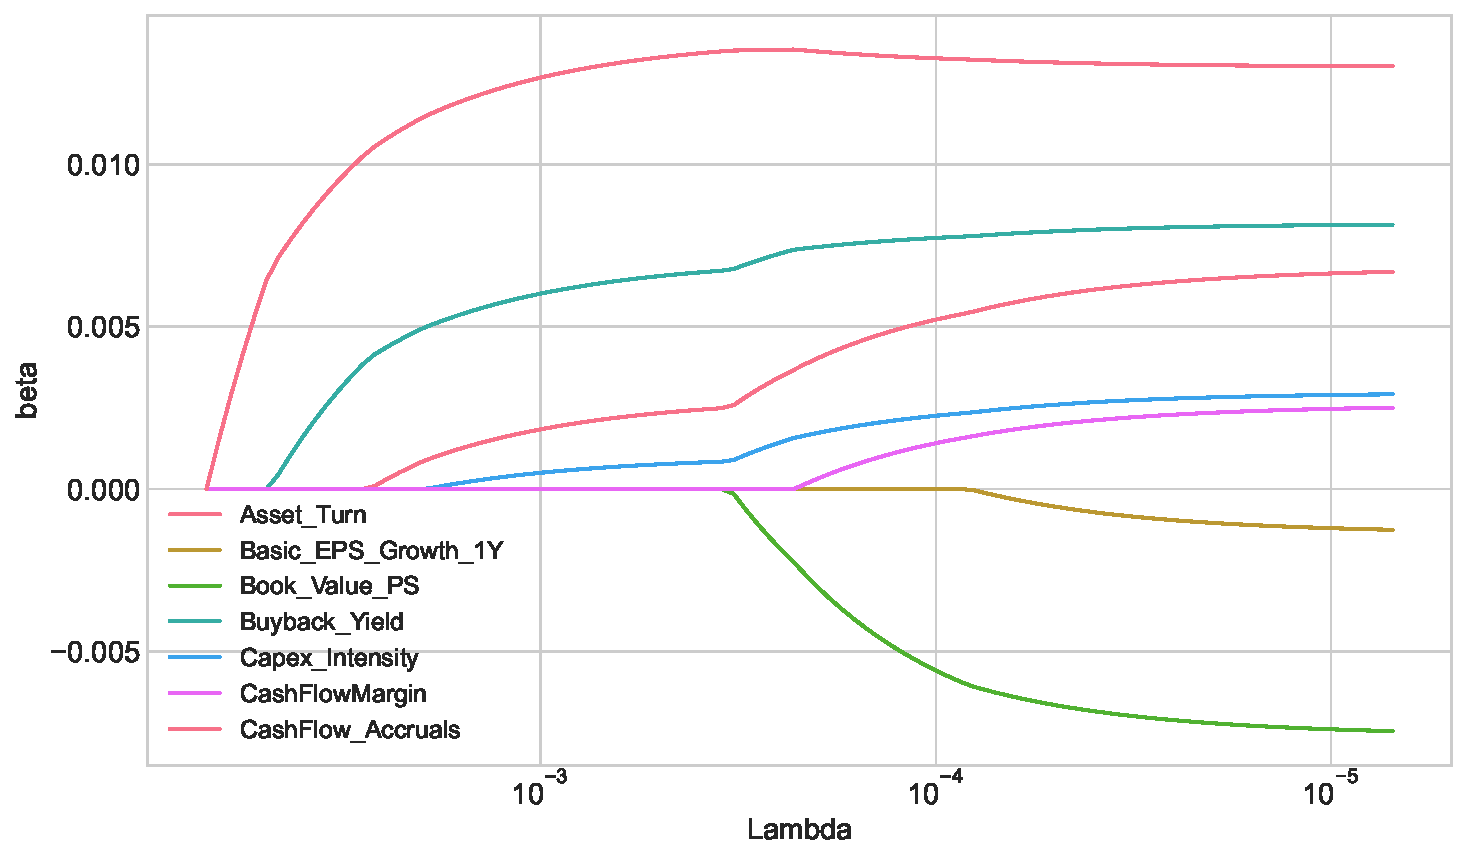
\includegraphics[width=0.7\linewidth]{files/f150ddf792902825185763e420f46789.pdf}}
\label{fig-lasso_plot}
\end{figure}

The graph plots the evolution of coefficients as the penalization intensity,{\textbackslash}index\{penalization intensity\} $\lambda$, increases. For some characteristics, like Asset Turnover (in green), the convergence to zero is rapid. Other variables resist the penalization longer, like Capex Assets, which is the last one to vanish. Essentially, this means that at the first order, this variable is an important driver of future 1-month returns in our sample.

Next, we turn to ridge regressions.

\begin{figure}[!htbp]
\centering
\begin{verbatim}
alphas_ridge = np.logspace(-2, 6, 100)  # Range of regularization values
coefs_ridge = []

for alpha in alphas_ridge:
    ridge = Ridge(alpha=alpha, fit_intercept=True)
    ridge.fit(x_penalized, y_penalized)
    coefs_ridge.append(ridge.coef_)

coefs_ridge = np.array(coefs_ridge)  # Shape: (n_alphas, n_features)

# Plot Ridge coefficients
plt.rcParams.update({'font.size': 14})
plt.figure(figsize=(10, 6))
for i in range(n_features_to_plot):
    plt.plot(alphas_ridge, coefs_ridge[:, i], label=features[i])

plt.xlabel('Lambda')
plt.ylabel('beta')
plt.legend(fontsize=12, loc='best', facecolor='white')
plt.xscale('log')
plt.tight_layout()
plt.show()
\end{verbatim}
\caption[]{Ridge coefficients. The dependent variable is the 1 month ahead return

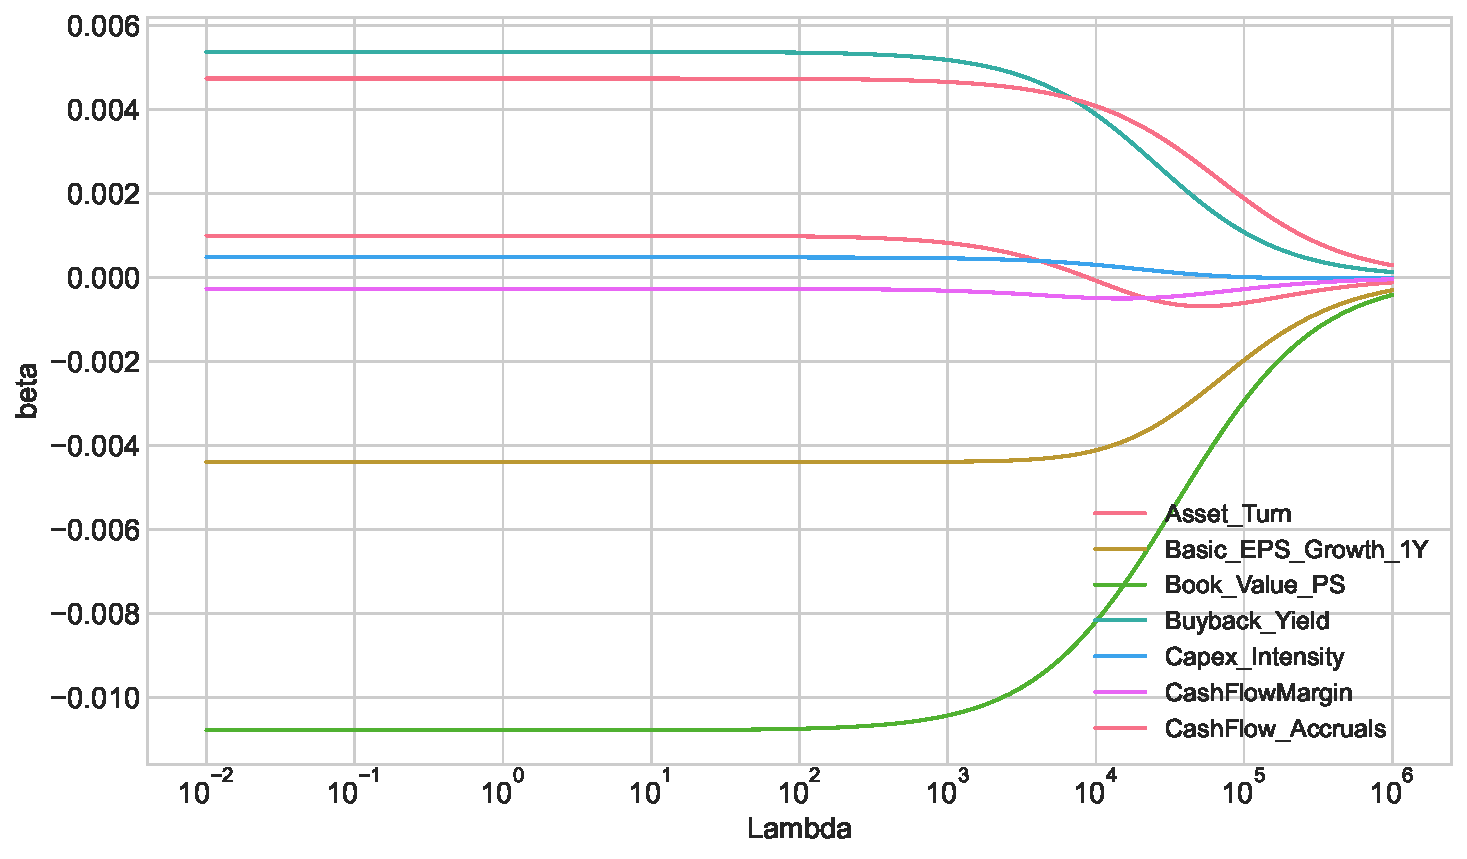
\includegraphics[width=0.7\linewidth]{files/63d9aff4078196cba6bb154fcaef66e3.pdf}}
\label{fig-ridge_plot}
\end{figure}

In Figure @ref(fig:sparseridge), the convergence to zero is much smoother. We underline that the x-axis (penalization intensities) have a log-scale. This allows to see the early patterns (close to zero, to the left) more clearly. As in the previous figure, the Mkt\_Cap\_3M\_Usd predictor clearly dominates, with again large negative coefficients. Nonetheless, as $\lambda$ increases, its domination over the other predictor fades.

By definition, the elasticnet will produce curves that behave like a blend of the two above approaches. Nonetheless, as long as $\alpha >0$, the selective property of the LASSO will be preserved: some features will see their coefficients shrink rapidly to zero. In fact, the strength of the LASSO is such that a balanced mix of the two penalizations is not reached at $\alpha = 1/2$, but rather at a much smaller value (possibly below 0.1).

\subsubsection{Sparse hedging for minimum variance portfolios}

{\textbackslash}index\{sparse hedging\}

\paragraph{Presentation and derivations}

The idea of constructing sparse portfolios{\textbackslash}index\{sparse portfolios\} is not new per se (see, e.g., \cite{brodie2009sparse}, \cite{fastrich2015constructing}) and the link with the selective property of the LASSO is rather straightforward in classical quadratic programs. Note that the choice of the $L^1$ norm is imperative because when enforcing a simple $L^2$ norm, the diversification of the portfolio increases (see \cite{coqueret2015diversified}).

The idea behind this section stems from \cite{goto2015improving} but the cornerstone result was first published by \cite{stevens1998inverse} and we present it below. We provide details because the derivations are not commonplace in the literature.

In usual mean-variance allocations, one core ingredient is the inverse covariance matrix of assets $\mathbf{\Sigma}^{ -1}$. For instance, the maximum Sharpe ratio (MSR) portfolio is given by

\begin{equation}
(\#eq:MSR)
\mathbf{w}^{\text{MSR}}=\frac{\mathbf{\Sigma}^{-1}\boldsymbol{\mu}}{\mathbf{1}'\mathbf{\Sigma}^{-1}\boldsymbol{\mu}},
\end{equation}
where $\mathbf{\mu}$ is the vector of expected (excess) returns. Taking $\mathbf{\mu}=\mathbf{1}$ yields the minimum variance portfolio,{\textbackslash}index\{minimum variance portfolio\} which is agnostic in terms of the first moment of expected returns (and, as such, usually more robust than most alternatives which try to estimate $\boldsymbol{\mu}$ and often fail).

Usually, the traditional way is to estimate $\boldsymbol{\Sigma}$ and to invert it to get the MSR weights. However, several approaches aim at estimating $\boldsymbol{\Sigma}^{ -1}$ {\textbackslash}textit\{directly\} and we present one of them below. We proceed one asset at a time, that is, one line of $\boldsymbol{\Sigma}^{ -1}$ at a time.\newline
If we decompose the matrix $\mathbf{\Sigma}$ into:
\begin{equation}
\mathbf{\Sigma}= \left[\begin{array}{cc} \sigma^2 & \mathbf{c}' \\
\mathbf{c}& \mathbf{C}\end{array} \right],
\end{equation}
classical partitioning results (e.g., Schur complements) imply
\$\${\textbackslash}small {\textbackslash}mathbf\{{\textbackslash}Sigma\}\^\{-1\}= {\textbackslash}left[{\textbackslash}begin\{array\}\{cc\} ({\textbackslash}sigma\^2 -{\textbackslash}mathbf\{c\}`{\textbackslash}mathbf\{C\}\^\{-1\}{\textbackslash}mathbf\{c\})\^\{-1\} \& - ({\textbackslash}sigma\^2 -{\textbackslash}mathbf\{c\}'{\textbackslash}mathbf\{C\}\^\{-1\}{\textbackslash}mathbf\{c\})\^\{-1\}{\textbackslash}mathbf\{c\}'{\textbackslash}mathbf\{C\}\^\{-1\} {\textbackslash}

\begin{itemize}
\item ({\textbackslash}sigma\^2 -{\textbackslash}mathbf\{c\}`{\textbackslash}mathbf\{C\}\^\{-1\}{\textbackslash}mathbf\{c\})\^\{-1\}{\textbackslash}mathbf\{C\}\^\{-1\}{\textbackslash}mathbf\{c\}\& {\textbackslash}mathbf\{C\}\^\{-1\}+ ({\textbackslash}sigma\^2 -{\textbackslash}mathbf\{c\}'{\textbackslash}mathbf\{C\}\^\{-1\}{\textbackslash}mathbf\{c\})\^\{-1\}{\textbackslash}mathbf\{C\}\^\{-1\}{\textbackslash}mathbf\{cc\}`{\textbackslash}mathbf\{C\}\^\{-1\}{\textbackslash}end\{array\} {\textbackslash}right].\$$We are interested in the first line, which has 2 components: the factor$({\textbackslash}sigma\^2 -{\textbackslash}mathbf\{c\}'{\textbackslash}mathbf\{C\}\^\{-1\}{\textbackslash}mathbf\{c\})\^\{-1\}$and the line vector${\textbackslash}mathbf\{c\}'{\textbackslash}mathbf\{C\}\^\{-1\}$.${\textbackslash}mathbf\{C\}$is the covariance matrix of assets$2$to$N$and${\textbackslash}mathbf\{c\}$is the covariance between the first asset and all other assets. The first line of${\textbackslash}mathbf\{{\textbackslash}Sigma\}\^\{-1\}\$ is
\end{itemize}
\begin{equation}
(\#eq:sparse1)
(\sigma^2 -\mathbf{c}'\mathbf{C}^{-1}\mathbf{c})^{-1} \left[1 \quad  \underbrace{-\mathbf{c}'\mathbf{C}^{-1}}_{N-1 \text{ terms}} \right].
\end{equation}

We now consider an alternative setting. We regress the returns of the first asset on those of all other assets:
\begin{equation}
(\#eq:sparseeq)
r_{1,t}=a_1+\sum_{n=2}^N\beta_{1|n}r_{n,t}+\epsilon_t, \quad \text{ i.e., } \quad  \mathbf{r}_1=a_1\mathbf{1}_T+\mathbf{R}_{-1}\mathbf{\beta}_1+\epsilon_1,
\end{equation}
where $\mathbf{R}_{ -1}$ gathers the returns of all assets except the first one. The OLS estimator for $\mathbf{\beta}_1$ is
\begin{equation}
(\#eq:sparse2)
\hat{\mathbf{\beta}}_{1}=\mathbf{C}^{-1}\mathbf{c},
\end{equation}

and this is the partitioned form (when a constant is included to the regression) stemming from the Frisch-Waugh-Lovell theorem (see chapter 3 in \cite{greene2018econometric}).

In addition,
\begin{equation}
(\#eq:sparse3)
(1-R^2)\sigma_{\mathbf{r}_1}^2=\sigma_{\mathbf{r}_1}^2- \mathbf{c}'\mathbf{C}^{-1}\mathbf{c} =\sigma^2_{\epsilon_1}.
\end{equation}
The proof of this last fact is given below.

With $\mathbf{X}$ being the concatenation of $\mathbf{1}_T$ with returns $\mathbf{R}_{ -1}$ and with $\mathbf{y}=\mathbf{r}_1$, the classical expression of the $R^2$ is
\begin{equation}
R^2=1-\frac{\mathbf{\epsilon}'\mathbf{\epsilon}}{T\sigma_Y^2}=1-\frac{\mathbf{y}'\mathbf{y}-\hat{\mathbf{\beta}'}\mathbf{X}'\mathbf{X}\hat{\mathbf{\beta}}}{T\sigma_Y^2}=1-\frac{\mathbf{y}'\mathbf{y}-\mathbf{y}'\mathbf{X}\hat{\mathbf{\beta}}}{T\sigma_Y^2},
\end{equation}
with fitted values $\mathbf{X}\hat{\mathbf{\beta}}= \hat{a_1}\mathbf{1}_T+\mathbf{R}_{ -1}\mathbf{C}^{ -1}\mathbf{c}$. Hence,
\begin{align*}
T\sigma_{\mathbf{r}_1}^2R^2&=T\sigma_{\mathbf{r}_1}^2-\mathbf{r}'_1\mathbf{r}_1+\hat{a_1}\mathbf{1}'_T\mathbf{r}_1+\mathbf{r}'_1\mathbf{R}_{-1}\mathbf{C}^{-1}\mathbf{c} \\
T(1-R^2)\sigma_{\mathbf{r}_1}^2&=\mathbf{r}'_1\mathbf{r}_1-\hat{a_1}\mathbf{1}'_T\mathbf{r}_1-\left(\mathbf{\tilde{r}}_1+\frac{\mathbf{1}_T\mathbf{1}'_T}{T}\mathbf{r}_1\right)'\left(\tilde{\mathbf{R}}_{-1}+\frac{\mathbf{1}_T\mathbf{1}'_T}{T}\mathbf{R}_{-1}\right)\mathbf{C}^{-1}\mathbf{c} \\
T(1-R^2)\sigma_{\mathbf{r}_1}^2&=\mathbf{r}'_1\mathbf{r}_1-\hat{a_1}\mathbf{1}'_T\mathbf{r}_1-T\mathbf{c}'\mathbf{C}^{-1}\mathbf{c} -\mathbf{r}'_1\frac{\mathbf{1}_T\mathbf{1}'_T}{T}\mathbf{R}_{-1} \mathbf{C}^{-1}\mathbf{c} \\
T(1-R^2)\sigma_{\mathbf{r}_1}^2&=\mathbf{r}'_1\mathbf{r}_1-\frac{(\mathbf{1}'_T\mathbf{r}_1)^2}{T}- T\mathbf{c}'\mathbf{C}^{-1}\mathbf{c} \\
(1-R^2)\sigma_{\mathbf{r}_1}^2&=\sigma_{\mathbf{r}_1}^2- \mathbf{c}'\mathbf{C}^{-1}\mathbf{c} 
\end{align*}
where in the fourth equality we have plugged $\hat{a}_1=\frac{\mathbf{1'}_T}{T}(\mathbf{r}_1 -\mathbf{R}_{ -1}\mathbf{C}^{ -1}\mathbf{c})$. Note that there is probably a simpler proof, see, e.g., section 3.5 in \cite{greene2018econometric}.

Combining (@ref(eq:sparse1), (@ref(eq:sparse2)) and (@ref(eq:sparse3)), we get that the first line of $\mathbf{\Sigma}^{ -1}$ is equal to
\begin{equation}
(\#eq:sparsehedgeeq2)
\frac{1}{\sigma^2_{\epsilon_1}}\times \left[ 1 \quad  -\hat{\boldsymbol{\beta}}_1'\right].
\end{equation}

Given the first line of $\mathbf{\Sigma}^{ -1}$, it suffices to multiply by $\boldsymbol{\mu}$ to get the portfolio weight in the first asset (up to a scaling constant).

There is a nice economic intuition behind the above results which justifies the term ``sparse hedging''.{\textbackslash}index\{sparse hedging\} We take the case of the minimum variance portfolio,{\textbackslash}index\{minimum variance portfolio\} for which $\boldsymbol{\mu}=\boldsymbol{1}$. In Equation @ref(eq:sparseeq), we try to explain the return of asset 1 with that of all other assets. In the above equation, up to a scaling constant, the portfolio has a unit position in the first asset and $-\hat{\boldsymbol{\beta}}_1$ positions in all other assets. Hence, the purpose of all other assets is clearly to hedge the return of the first one. In fact, these positions are aimed at minimizing the squared errors of the aggregate portfolio for the first asset (these errors are exactly $\mathbf{\epsilon}_1$). Moreover, the scaling factor $\sigma^{ -2}_{\epsilon_1}$ is also simple to interpret: the more we trust the regression output (because of a small $\sigma^{2}_{\epsilon_1}$), the more we invest in the hedging portfolio of the asset.

This reasoning is easily generalized for any line of $\mathbf{\Sigma}^{ -1}$, which can be obtained by regressing the returns of asset $i$ on the returns of all other assets. If the allocation scheme has the form (@ref(eq:MSR)) for given values of $\boldsymbol{\mu}$, then the pseudo-code for the sparse portfolio strategy is the following.

At each date (which we omit for notational convenience),

\begin{itemize}
\item For all stocks $i$,
\end{itemize}

\begin{enumerate}
\item estimate the elasticnet regression over the $t=1,\dots,T$ samples to get the $i^{th}$ line of $\hat{\mathbf{\Sigma}}^{ -1}$:

\begin{equation}
\small \left[\hat{\mathbf{\Sigma}}^{-1}\right]_{i,\cdot}= \underset{\mathbf{\beta}_{i|}}{\text{argmin}}\, \left\{\sum_{t=1}^T\left( r_{i,t}-a_i+\sum_{n\neq i}^N\beta_{i|n}r_{n,t}\right)^2+\lambda \alpha ||  \mathbf{\beta}_{i|}||_1+\lambda (1-\alpha)||\mathbf{\beta}_{i|}||_2^2\right\}
\end{equation}


\item to get the weights of asset $i$, we compute the $\mathbf{\mu}$-weighted sum:
$w_i= \sigma_{\epsilon_i}^{ -2}\left(\mu_i - \sum_{j\neq i}\mathbf{\beta}_{i|j}\mu_j\right)$,
\end{enumerate}

where we recall that the vectors $\mathbf{\beta}_{i|}=[\mathbf{\beta}_{i|1},\dots,\mathbf{\beta}_{i|i -1},\mathbf{\beta}_{i|i+1},\dots,\mathbf{\beta}_{i|N}]$ are the coefficients from regressing the returns of asset $i$ against the returns of all other assets.\newline
The introduction of the \textbf{penalization norms} is the new ingredient, compared to the original approach of \cite{stevens1998inverse}. The benefits are twofold: first, introducing constraints yields weights that are more robust and less subject to errors in the estimates of $\mathbf{\mu}$; second, because of sparsity, weights are more stable, less leveraged and thus the strategy is less impacted by transaction costs. Before we turn to numerical applications, we mention a more direct route to the estimation of a \textbf{robust inverse covariance matrix}: the Graphical LASSO. The GLASSO estimates the precision matrix (inverse covariance matrix) via maximum likelihood while imposing constraints/penalizations on the weights of the matrix. When the penalization is strong enough, this yields a sparse matrix, i.e., a matrix in which some and possibly many coefficients are zero. We refer to the original article \cite{friedman2008sparse} for more details on this subject.

\paragraph{Example}\label{sparseex}

The interest of sparse hedging portfolios{\textbackslash}index\{sparse hedging\} is to propose a robust approach to the estimation of minimum variance policies.{\textbackslash}index\{minimum variance portfolio\} Indeed, since the vector of expected returns $\boldsymbol{\mu}$ is usually very noisy, a simple solution is to adopt an agnostic view by setting $\boldsymbol{\mu}=\boldsymbol{1}$. In order to test the added value of the sparsity constraint, we must resort to a full backtest.{\textbackslash}index\{backtest\} In doing so, we anticipate the content of Chapter \href{/chap-15-portfolio-backtesting}{Portfolio backtesting}.

We first prepare the variables. Sparse portfolios are based on returns only; we thus base our analysis on the dedicated variable in matrix/rectangular format (\textit{returns}) which were created at the end of Chapter @ref(notdata).

Then, we initialize the output variables: portfolio weights and portfolio returns. We want to compare three strategies: an equally weighted (EW){\textbackslash}index\{equally weighted portfolio\} benchmark of all stocks, the classical global minimum variance portfolio (GMV) and the sparse-hedging approach to minimum variance.

\begin{verbatim}
# Out-of-sample dates
t_oos = returns.loc[returns['date'] > separation_date, 'date'].unique()
t_oos = pd.to_datetime(t_oos)                                          # Transform to datetime format

Tt = len(t_oos)                                                        # Nb of dates
nb_port = 3                                                            # Nb of portfolios/strats.
n_assets = returns.shape[1] - 1                                        # Number of assets (excluding date)
portf_weights = np.zeros((Tt, nb_port, n_assets))                      # Initial portf. weights
portf_returns = np.zeros((Tt, nb_port))                                # Initial portf. returns
\end{verbatim}

Next, because it is the purpose of this section, we isolate the computation of the weights of sparse-hedging portfolios. In the case of minimum variance portfolios, when $\boldsymbol{\mu}=\boldsymbol{1}$, the weight in asset 1 will simply be the sum of all terms in Equation @ref(eq:sparsehedgeeq2) and the other weights have similar forms.

\begin{verbatim}
def weights_sparsehedge(returns, alpha, lambda_param):  # The parameters are defined here
    """Compute sparse hedging portfolio weights."""
    n_assets = returns.shape[1]
    w = np.zeros(n_assets)                              # Initiate weights
    
    for i in range(n_assets):                           # Loop on the assets
        y = returns[:, i]                               # Dependent variable
        x = np.delete(returns, i, axis=1)               # Independent variables (all except i)
        
        # ElasticNet in sklearn: alpha = lambda, l1_ratio = alpha (mixing parameter)
        fit = ElasticNet(alpha=lambda_param, l1_ratio=alpha, fit_intercept=True)
        fit.fit(x, y)
        
        err = y - fit.predict(x)                        # Prediction errors
        w[i] = (1 - np.sum(fit.coef_)) / np.var(err)    # Output: weight of asset i
    
    return w / np.sum(w)                                # Normalisation of weights
\end{verbatim}

We define a meta-weighting function that embeds three strategies.

\begin{verbatim}
def weights_multi(returns, j, alpha, lambda_param):
    """Compute portfolio weights for different strategies."""
    N = returns.shape[1]
    
    if j == 1:                                          # j = 1 => EW
        return np.ones(N) / N
    
    if j == 2:                                          # j = 2 => Minimum Variance
        sigma = np.cov(returns, rowvar=False) + 0.01 * np.eye(N)  # Covariance matrix + regularizing term
        w = np.linalg.solve(sigma, np.ones(N))          # Inverse & multiply
        return w / np.sum(w)                            # Normalize
    
    if j == 3:                                          # j = 3 => Penalised / elasticnet
        return weights_sparsehedge(returns, alpha, lambda_param)
\end{verbatim}

Finally, we proceed to the backtesting loop.

\begin{verbatim}
for t in range(len(t_oos)):                                              # Loop = rebal. dates
    # Data for weights (expanding window)
    temp_data = returns.loc[returns['date'] < t_oos[t]].drop(columns='date').values
    
    # OOS returns
    realised_returns = returns.loc[returns['date'] == t_oos[t]].drop(columns='date').values.flatten()
    
    for j in range(1, nb_port + 1):                                      # Loop over strats
        portf_weights[t, j-1, :] = weights_multi(temp_data, j, 0.03, 0.03) # Hard-coded params!
        portf_returns[t, j-1] = np.sum(portf_weights[t, j-1, :] * realised_returns)  # Portf. returns

# Convert to DataFrame with column names
portf_returns_df = pd.DataFrame(portf_returns, columns=["EW", "MV", "Sparse"])

# Portfolio volatilities (monthly scale)
print(portf_returns_df.std())
\end{verbatim}

\begin{verbatim}
EW        0.055929
MV        0.032911
Sparse    0.043544
dtype: float64
\end{verbatim}

The aim of the sparse hedging{\textbackslash}index\{sparse hedging\} restrictions is to provide a better estimate of the covariance structure of assets so that the estimation of minimum variance portfolio weights is more accurate. From the above exercise, we see that the monthly volatility is indeed reduced when building covariance matrices based on sparse hedging relationships. This is not the case if we use the shrunk sample covariance matrix because there is probably too much noise in the estimates of correlations between assets. Working with daily returns would likely improve the quality of the estimates. But the above backtest shows that the penalized methodology performs well even when the number of observations (dates) is small compared to the number of assets.

\subsubsection{Predictive regressions}

{\textbackslash}index\{predictive regression\}

\paragraph{Literature review and principle}

The topic of predictive regressions sits on a collection of very interesting articles. One influential contribution is \cite{stambaugh1999predictive}, where the author shows the perils of regressions in which the independent variables are autocorrelated. In this case, the usual OLS estimate is biased and must therefore be corrected. The results have since then been extended in numerous directions (see \cite{campbell2006efficient} and \cite{hjalmarsson2011new}, the survey in \cite{gonzalo2018predictive} and, more recently, the study of \cite{xu2020testing} on predictability over multiple horizons).

A second important topic pertains to the time-dependence of the coefficients in predictive regressions. One contribution in this direction is \cite{dangl2012predictive}, where coefficients are estimated via a Bayesian procedure. More recently \cite{kelly2019characteristics} use time-dependent factor loadings to model the cross-section of stock returns. The time-varying nature of coefficients of predictive regressions is further documented by \cite{henkel2011time} for short term returns. Lastly, \cite{farmer2019pockets} introduce the concept of pockets of predictability: assets or markets experience different phases; in some stages, they are predictable and in some others, they aren't. Pockets are measured both by the number of days that a \textit{t}-statistic is above a particular threshold and by the magnitude of the $R^2$ over the considered period. Formal statistical tests are developed by \cite{demetrescu2020testing}.

The introduction of penalization within predictive regressions goes back at least to \cite{rapach2013international}, where they are used to assess lead-lag relationships between US markets and other international stock exchanges.{\textbackslash}index\{penalized regression\} More recently, \cite{chinco2019sparse} use LASSO regressions to forecast high frequency returns based on past returns (in the cross-section) at various horizons. They report statistically significant gains. \cite{han2018firm} and \cite{rapach2019time} use LASSO and elasticnet regressions (respectively) to improve forecast combinations and single out the characteristics that matter when explaining stock returns. Recently, \cite{lee2022lasso} introduce small variations on the LASSO aimed at improving coefficient estimation consistency.

These contributions underline the relevance of the overlap between predictive regressions{\textbackslash}index\{penalized regression\} and penalized regressions. In simple machine-learning based asset pricing, we often seek to build models such as that of Equation @ref(eq:genML). If we stick to a linear relationship and add penalization terms, then the model becomes:
\begin{equation}
r_{t+1,n} = \alpha_n + \sum_{k=1}^K\beta_n^kf^k_{t,n}+\epsilon_{t+1,n}, \quad \text{s.t.} \quad (1-\alpha)\sum_{j=1}^J |\beta_j| +\alpha\sum_{j=1}^J \beta_j^2< \theta
\end{equation}
where we use $f^k_{t,n}$ or $x_{t,n}^k$ interchangeably and $\theta$ is some penalization intensity. Again, one of the aims of the regularization is to generate more robust estimates. If the patterns extracted hold out of sample, then
\begin{equation}
\hat{r}_{t+1,n} = \hat{\alpha}_n + \sum_{k=1}^K\hat{\beta}_n^kf^k_{t,n},
\end{equation}
will be a relatively reliable proxy of future performance.

\paragraph{Code and results}

Given the form of our dataset, implementing penalized predictive regressions is easy.

\begin{verbatim}
training_sample = data_ml[data_ml['date'] <= separation_date].dropna(subset=(features_short + ['R1M']))
testing_sample = data_ml[data_ml['date'] > separation_date].dropna(subset=(features_short + ['R1M']))

y_penalized_train = training_sample['R1M'].values                  # Dependent variable
x_penalized_train = training_sample[features_short].values                   # Predictors

# Model: ElasticNet with alpha (lambda) = 0.1 and l1_ratio (alpha) = 0.1
fit_pen_pred = ElasticNet(alpha=0.1, l1_ratio=0.1, fit_intercept=True)
fit_pen_pred.fit(x_penalized_train, y_penalized_train)
\end{verbatim}

\begin{verbatim}
ElasticNet(alpha=0.1, l1_ratio=0.1)
\end{verbatim}

We then report two key performance measures: the mean squared error and the hit ratio, which is the proportion of times that the prediction guesses the sign of the return correctly. A detailed account of metrics is given later in the book (Chapter \href{/chap-15-portfolio-backtesting}{Portfolio backtesting}).

\begin{verbatim}
x_penalized_test = testing_sample[features_short].values                     # Predictors
y_test = testing_sample['R1M'].values

predictions = fit_pen_pred.predict(x_penalized_test)

# MSE
mse = np.mean((predictions - y_test) ** 2)
print(f"MSE: {mse}")

# Hit ratio
hit_ratio = np.mean(predictions * y_test > 0)
print(f"Hit ratio: {hit_ratio}")
\end{verbatim}

\begin{verbatim}
MSE: 0.015580212568421932
Hit ratio: 0.5385195821306648
\end{verbatim}

\subsubsection{Coding exercise}

On the test sample, evaluate the impact of the two elastic net parameters on out-of-sample accuracy.

\subsection{Tree-based methods}

Classification and regression trees are simple yet powerful clustering algorithms popularized by the monograph of \cite{breiman1984classification}. Decision trees and their extensions are known to be quite efficient forecasting tools when working on tabular data. A large proportion of winning solutions in ML contests (especially on the Kaggle website\footnote{See \href{http://www.kaggle.com}{www.kaggle.com}.}) resort to improvements of simple trees. For instance, the meta-study in bioinformatics by \cite{olson2018data} finds that boosted trees and random forests are the top 2 algorithms from a group of 13, excluding neural networks.

Recently, the surge in Machine Learning applications in Finance has led to multiple publications that use trees in portfolio allocation problems. A long, though not exhaustive, list includes: \cite{ballings2015evaluating}, \cite{patel2015predicting}, \cite{patel2015bpredicting}, \cite{moritz2016tree}, \cite{krauss2017deep}, \cite{gu2018empirical}, \cite{guida2019big}, \cite{coqueret2019training} and \cite{simonian2019machine}. One notable contribution is \cite{bryzgalova2019forest} in which the authors create factors from trees by sorting portfolios via simple trees, which they call \textit{Asset Pricing Trees}. Another recent article \citep{he2021panel} seeks to create global splitting criteria for the purpose of asset pricing.

In this chapter, we review the methodologies associated to trees and their applications in portfolio choice.

\subsubsection{Simple trees}

\paragraph{Principle}

Decision trees seek to partition datasets into \textbf{homogeneous clusters}. Given an exogenous variable $\mathbf{Y}$ and features $\mathbf{X}$, trees iteratively split the sample into groups (usually two at a time) which are as homogeneous in $\mathbf{Y}$ as possible. The splits are made according to one variable within the set of features. A short word on nomenclature: when $\mathbf{Y}$ consists of real numbers, we talk about \textit{regression trees} and when $\mathbf{Y}$ is categorical, we use the term \textit{classification trees}.

Before formalizing this idea, we illustrate this process in Figure~\ref{fig-tree_scheme}. There are 12 stars with three features: color, size and complexity (number of branches).

\begin{figure}[!htbp]
\centering
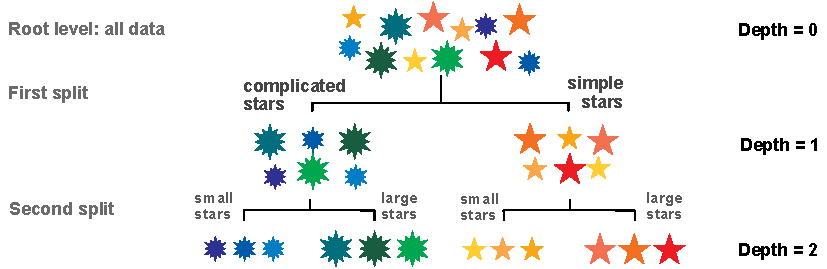
\includegraphics[width=0.7\linewidth]{files/tree_scheme-647f9559483861e05198b4e2b3953caf.pdf}
\caption[]{Pedagogical diagram of a tree.}
\label{fig-tree_scheme}
\end{figure}

The dependent variable is the color (let's consider the wavelength associated to the color for simplicity). The first split is made according to size or complexity. Clearly, complexity is the better choice: complicated stars are blue and green, while simple stars are yellow, orange and red. Splitting according to size would have mixed blue and yellow stars (small ones) and green and orange stars (large ones).

The second step is to split the two clusters one level further. Since only one variable (size) is relevant, the secondary splits are straightforward. In the end, our stylized tree has four consistent clusters. The analogy with factor investing is simple: the color represents performance: red for high performance and blue for mediocre performance. The features (size and complexity of stars) are replaced by firm-specific attributes, such as capitalization, accounting ratios, etc. Hence, the purpose of the exercise is to find the characteristics that allow to split firms into the ones that will perform well versus those likely to fare more poorly.

We now turn to the technical construction of regression trees (splitting process). We follow the standard literature as exposed in \cite{breiman1984classification} or in chapter 9 of \cite{friedman2009elements}. Given a sample of ($y_i$,$\mathbf{x}_i$) of size $I$, a \textit{regression} tree seeks the splitting points that minimize the total variation of the $y_i$ inside the two child clusters. These two clusters need not have the same size. In order to do that, it proceeds in two steps. First, it finds, for each feature $x_i^{(k)}$, the best splitting point (so that the clusters are homogeneous in $\mathbf{Y}$). Second, it selects the feature that achieves the highest level of homogeneity.

Homogeneity in regression trees is closely linked to variance. Since we want the $y_i$ inside each cluster to be similar, we seek to \textbf{minimize their variability} (or \textbf{dispersion}) inside each cluster and then sum the two figures. We cannot sum the variances because this would not take into account the relative sizes of clusters. Hence, we work with \textit{total} variation, which is the variance times the number of elements in the clusters.

Below, the notation is a bit heavy because we resort to superscripts $k$ (the index of the feature), but it is largely possible to ignore these superscripts to ease understanding. The first step is to find the best split for each feature, that is, solve $\underset{c^{(k)}}{\text{argmin}} \ V^{(k)}_I(c^{(k)})$ with

\begin{equation}
V^{(k)}_I(c^{(k)})= \underbrace{\sum_{x_i^{(k)}<c^{(k)}}\left(y_i-m_I^{k,-}(c^{(k)}) \right)^2}_{\text{Total dispersion of first cluster}} + \underbrace{\sum_{x_i^{(k)}>c^{(k)}}\left(y_i-m_I^{k,+}(c^{(k)}) \right)^2}_{\text{Total dispersion of second cluster}},
\end{equation}

where

\begin{equation}
\begin{aligned}
m_I^{k,-}(c^{(k)})&=\frac{1}{\#\{i,x_i^{(k)}<c^{(k)} \}}\sum_{\{x_i^{(k)}<c^{(k)} \}}y_i \quad \text{ and } \\ m_I^{k,+}(c^{(k)})&=\frac{1}{\#\{i,x_i^{(k)}>c^{(k)} \}}\sum_{\{x_i^{(k)}>c^{(k)} \}}y_i
\end{aligned}
\end{equation}

are the average values of $Y$, conditional on $X^{(k)}$ being smaller or larger than $c$. The cardinal function $\#\{\cdot\}$ counts the number of instances of its argument. For feature $k$, the optimal split $c^{k,*}$ is thus the one for which the total dispersion over the two subgroups is the smallest.

The optimal splits satisfy $c^{k,*}= \underset{c^{(k)}}{\text{argmin}} \ V^{(k)}_I(c^{(k)})$. Of all the possible splitting variables, the tree will choose the one that minimizes the total dispersion not only over all splits, but also over all variables: $k^*=\underset{k}{\text{argmin}} \ V^{(k)}_I(c^{k,*})$.

After one split is performed, the procedure continues on the two newly formed clusters. There are several criteria that can determine when to stop the splitting process (see Section @ref(pruning-criteria)). One simple criterion is to fix a maximum number of levels (the depth) for the tree. A usual condition is to impose a minimum gain that is expected for each split. If the reduction in dispersion after the split is only marginal and below a specified threshold, then the split is not executed. For further technical discussions on decision trees, we refer for instance to section 9.2.4 of \cite{friedman2009elements}.

When the tree is built (trained), a prediction for new instances is easy to make. Given its feature values, the instance ends up in one leaf of the tree. Each leaf has an average value for the label: this is the predicted outcome. Of course, this only works when the label is numerical. We discuss below the changes that occur when it is categorical.

\paragraph{Further details on classification}\label{sec_treeclass}

Classification exercises are somewhat more complex than regression tasks. The most obvious difference is the measure of dispersion or heterogeneity. This loss function which must take into account the fact that the final output is not a simple number, but a vector. The output $\tilde{\textbf{y}}_i$ has as many elements as there are categories in the label and each element is the probability that the instance belongs to the corresponding category.

For instance, if there are 3 categories: \textit{buy}, \textit{hold} and \textit{sell}, then each instance would have a label with as many columns as there are classes. Following our example, one label would be (1,0,0) for a \textit{buy} position for instance. We refer to Section @ref(categorical-labels) for a introduction on this topic.

Inside a tree, labels are aggregated at each cluster level. A typical output would look like (0.6,0.1,0.3): they are the proportions of each class represented within the cluster. In this case, the cluster has 60\% of \textit{buy}, 10\% of \textit{hold} and 30\% of \textit{sell}.

The loss function must take into account this multidimensionality of the label. When building trees, since the aim is to favor homogeneity, the loss penalizes outputs that are not concentrated towards one class. Indeed, facing a diversified output of (0.3,0.4,0.3) is much harder to handle than the concentrated case of (0.8,0.1,0.1).

The algorithm is thus seeking purity: it searches a splitting criterion that will lead to clusters that are as pure as possible, i.e., with one very dominant class, or at least just a few dominant classes. There are several metrics proposed by the literature and all are based on the proportions generated by the output. If there are $J$ classes, we denote these proportions with $p_j$. For each leaf, the usual loss functions are:

\begin{itemize}
\item the Gini impurity index: $1 -\sum_{j=1}^Jp_j^2;$
\item the misclassification error: $1 -\underset{j}{\text{max}}\, p_j;$
\item entropy: $-\sum_{j=1}^J\log(p_j)p_j.$
\end{itemize}

The Gini index is nothing but one minus the Herfindahl index which measures the diversification of a portfolio. Trees seek partitions that are the least diversified. The minimum value of the Gini index is zero and reached when one $p_j=1$ and all others are equal to zero. The maximum value is equal to $1 -1/J$ and is reached when all $p_j=1/J$. Similar relationships hold for the other two losses. One drawback of the misclassification error is its lack of differentiability which explains why the other two options are often favored.

Once the tree is grown, new instances automatically belong to one final leaf. This leaf is associated to the proportions of classes it nests. Usually, to make a prediction, the class with highest proportion (or probability) is chosen when a new instance is associated with the leaf.

\paragraph{Pruning criteria}

When building a tree, the splitting process can be pursued until the full tree is grown, that is, when:

\begin{itemize}
\item all instances belong to separate leaves, and/or
\item all leaves comprise instances that cannot be further segregated based on the current set of features.
\end{itemize}

At this stage, the splitting process cannot be pursued.

Obviously, fully grown trees often lead to almost perfect fits when the predictors are relevant, numerous and numerical. Nonetheless, the fine grained idiosyncrasies of the training sample are of little interest for out-of-sample predictions. For instance, being able to perfectly match the patterns of 2000 to 2006 will probably not be very interesting in the period from 2007 to 2009. The most reliable sections of the trees are those closest to the root because they embed large portions of the data: the average values in the early clusters are trustworthy because the are computed on a large number of observations. The first splits are those that matter the most because they determine the most general patterns. The deepest splits only deal with the peculiarities of the sample.

Thus, it is imperative to limit the size of the tree to avoid overfitting. There are several ways to prune the tree and all depend on some particular criteria. We list a few of them below:

\begin{itemize}
\item Impose a minimum number of instances for each terminal node (leaf). This ensures that each final cluster is composed of a sufficient number of observations. Hence, the average value of the label will be reliable because it is calculated on a large amount of data.
\item Similarly, it can be imposed that a cluster has a minimal size before even considering any further split. This criterion is of course related to the one above.
\item Require a certain threshold of improvement in the fit. If a split does not sufficiently reduce the loss, then it can be deemed unnecessary. The user specifies a small number $\epsilon>0$ and a split is only validated if the loss obtained post-split is smaller than $1 -\epsilon$ times the loss before the split.
\item Limit the depth of the tree. The depth is defined as the overal maximum number of splits between the root and any leaf of the tree.
\end{itemize}

In the example below, we implement all of these criteria at the same time, but usually, two of them at most should suffice.

\paragraph{Code and interpretation}

We start with a simple tree and its interpretation. We use the package \textit{scikit-learn} and its plotting engine. The label is the future 1-month return and the features are all predictors available in the sample. The tree is trained on the full sample.

\begin{verbatim}
from sklearn.tree import DecisionTreeRegressor, DecisionTreeClassifier, plot_tree
from sklearn.ensemble import RandomForestRegressor, RandomForestClassifier, AdaBoostClassifier
import lightgbm as lgb
import xgboost as xgb
import matplotlib.pyplot as plt
import numpy as np
import pandas as pd
import seaborn as sns
from scipy import stats
from statsmodels.tsa.stattools import acf
import warnings
warnings.filterwarnings('ignore')
plt.style.use('seaborn-v0_8-whitegrid')
sns.set_palette("husl")

# Building the data & import functions
from data_build import generate_data
data_ml, features, features_short, returns, stock_ids, stock_ids_short = generate_data()
features_short =["Div_yld", "EPS", "size_avg_252d", "mom_252", "OCF_Growth_1Y", "PB", "vol_252"]
separation_date = "2017-01-15"
data_ml_clean = data_ml.dropna(subset=(features + ['R1M']))
\end{verbatim}

There usually exists a convention in the representation of trees. At each node, a condition describes the split with a Boolean expression. If the expression is \textbf{true}, then the instance goes to the \textbf{left cluster}; if not, it goes to the \textit{right} cluster. Given the whole sample, the initial split in this tree (Figure @ref(fig:rpart1)) is performed according to the price-to-book ratio. If the Pb score (or value) of the instance is above 0.025, then the instance is placed in the left bucket; otherwise, it goes in the \textbf{right bucket}.

At each node, there are two important metrics. The first one is the average value of the label in the cluster, and the second one is the proportion of instances in the cluster. At the top of the tree, all instances (100\%) are present and the average 1-month future return is 1.3\%. One level below, the left cluster is by far the most crowded, with roughly 98\% of observations averaging a 1.2\% return. The right cluster is much smaller (2\%) but concentrates instances with a much higher average return (5.9\%). This is possibly an idiosyncracy of the sample.

The splitting process continues similarly at each node until some condition is satisfied (typically here: the maximum depth is reached). A color codes the average return: from white (low return) to blue (high return). The leftmost cluster with the lowest average return consists of firms that satisfy \textit{all} the following criteria:

\begin{itemize}
\item have a Pb score above 0.025;
\item have a 3-month market capitalization score above 0.16;
\item have a score of average daily volume over the past 3 months above 0.85.
\end{itemize}

Notice that one peculiarity of trees is their possible heterogeneity in cluster sizes. Sometimes, a few clusters gather almost all of the observations while a few small groups embed some outliers. This is not a favorable property of trees, as small groups are more likely to be flukes and may fail to generalize out-of-sample.

This is why we imposed restrictions during the construction of the tree. The first one (min\_samples\_leaf = 3500 in the code) imposes that each cluster consists of at least 3500 instances. The second one (min\_samples\_split) further imposes that a cluster comprises at least 8000 observations in order to pursue the splitting process. These values logically depend on the size of the training sample. The ccp\_alpha = 0.0001 parameter in the code requires any split to reduce the loss below 0.9999 times its original value before the split. Finally, the maximum depth of three essentially means that there are at most three splits between the root of the tree and any terminal leaf.

The complexity of the tree (measured by the number of terminal leaves) is a decreasing function of min\_samples\_leaf, min\_samples\_split and ccp\_alpha and an increasing function of maximum depth.

Once the model has been trained (i.e., the tree is grown), a prediction for any instance is the average value of the label within the cluster where the instance should land.

\begin{figure}[!htbp]
\centering
\begin{verbatim}
X = data_ml_clean[features]
y = data_ml_clean['R1M']

fit_tree = DecisionTreeRegressor(
    min_samples_leaf=350,   # Min nb of obs required in each terminal node (leaf)
    min_samples_split=800,  # Min nb of obs required to continue splitting
    ccp_alpha=0.0001,       # Complexity parameter: smaller = more leaves
    max_depth=4             # Maximum depth (i.e. tree levels)
)
fit_tree.fit(X, y)

# Plot the tree
plt.figure(figsize=(20, 10))
plot_tree(fit_tree, feature_names=features, filled=True, rounded=True)
plt.tight_layout()
plt.show()
\end{verbatim}
\caption[]{Simple characteristics-based tree. The dependent variable is the 1 month future return.

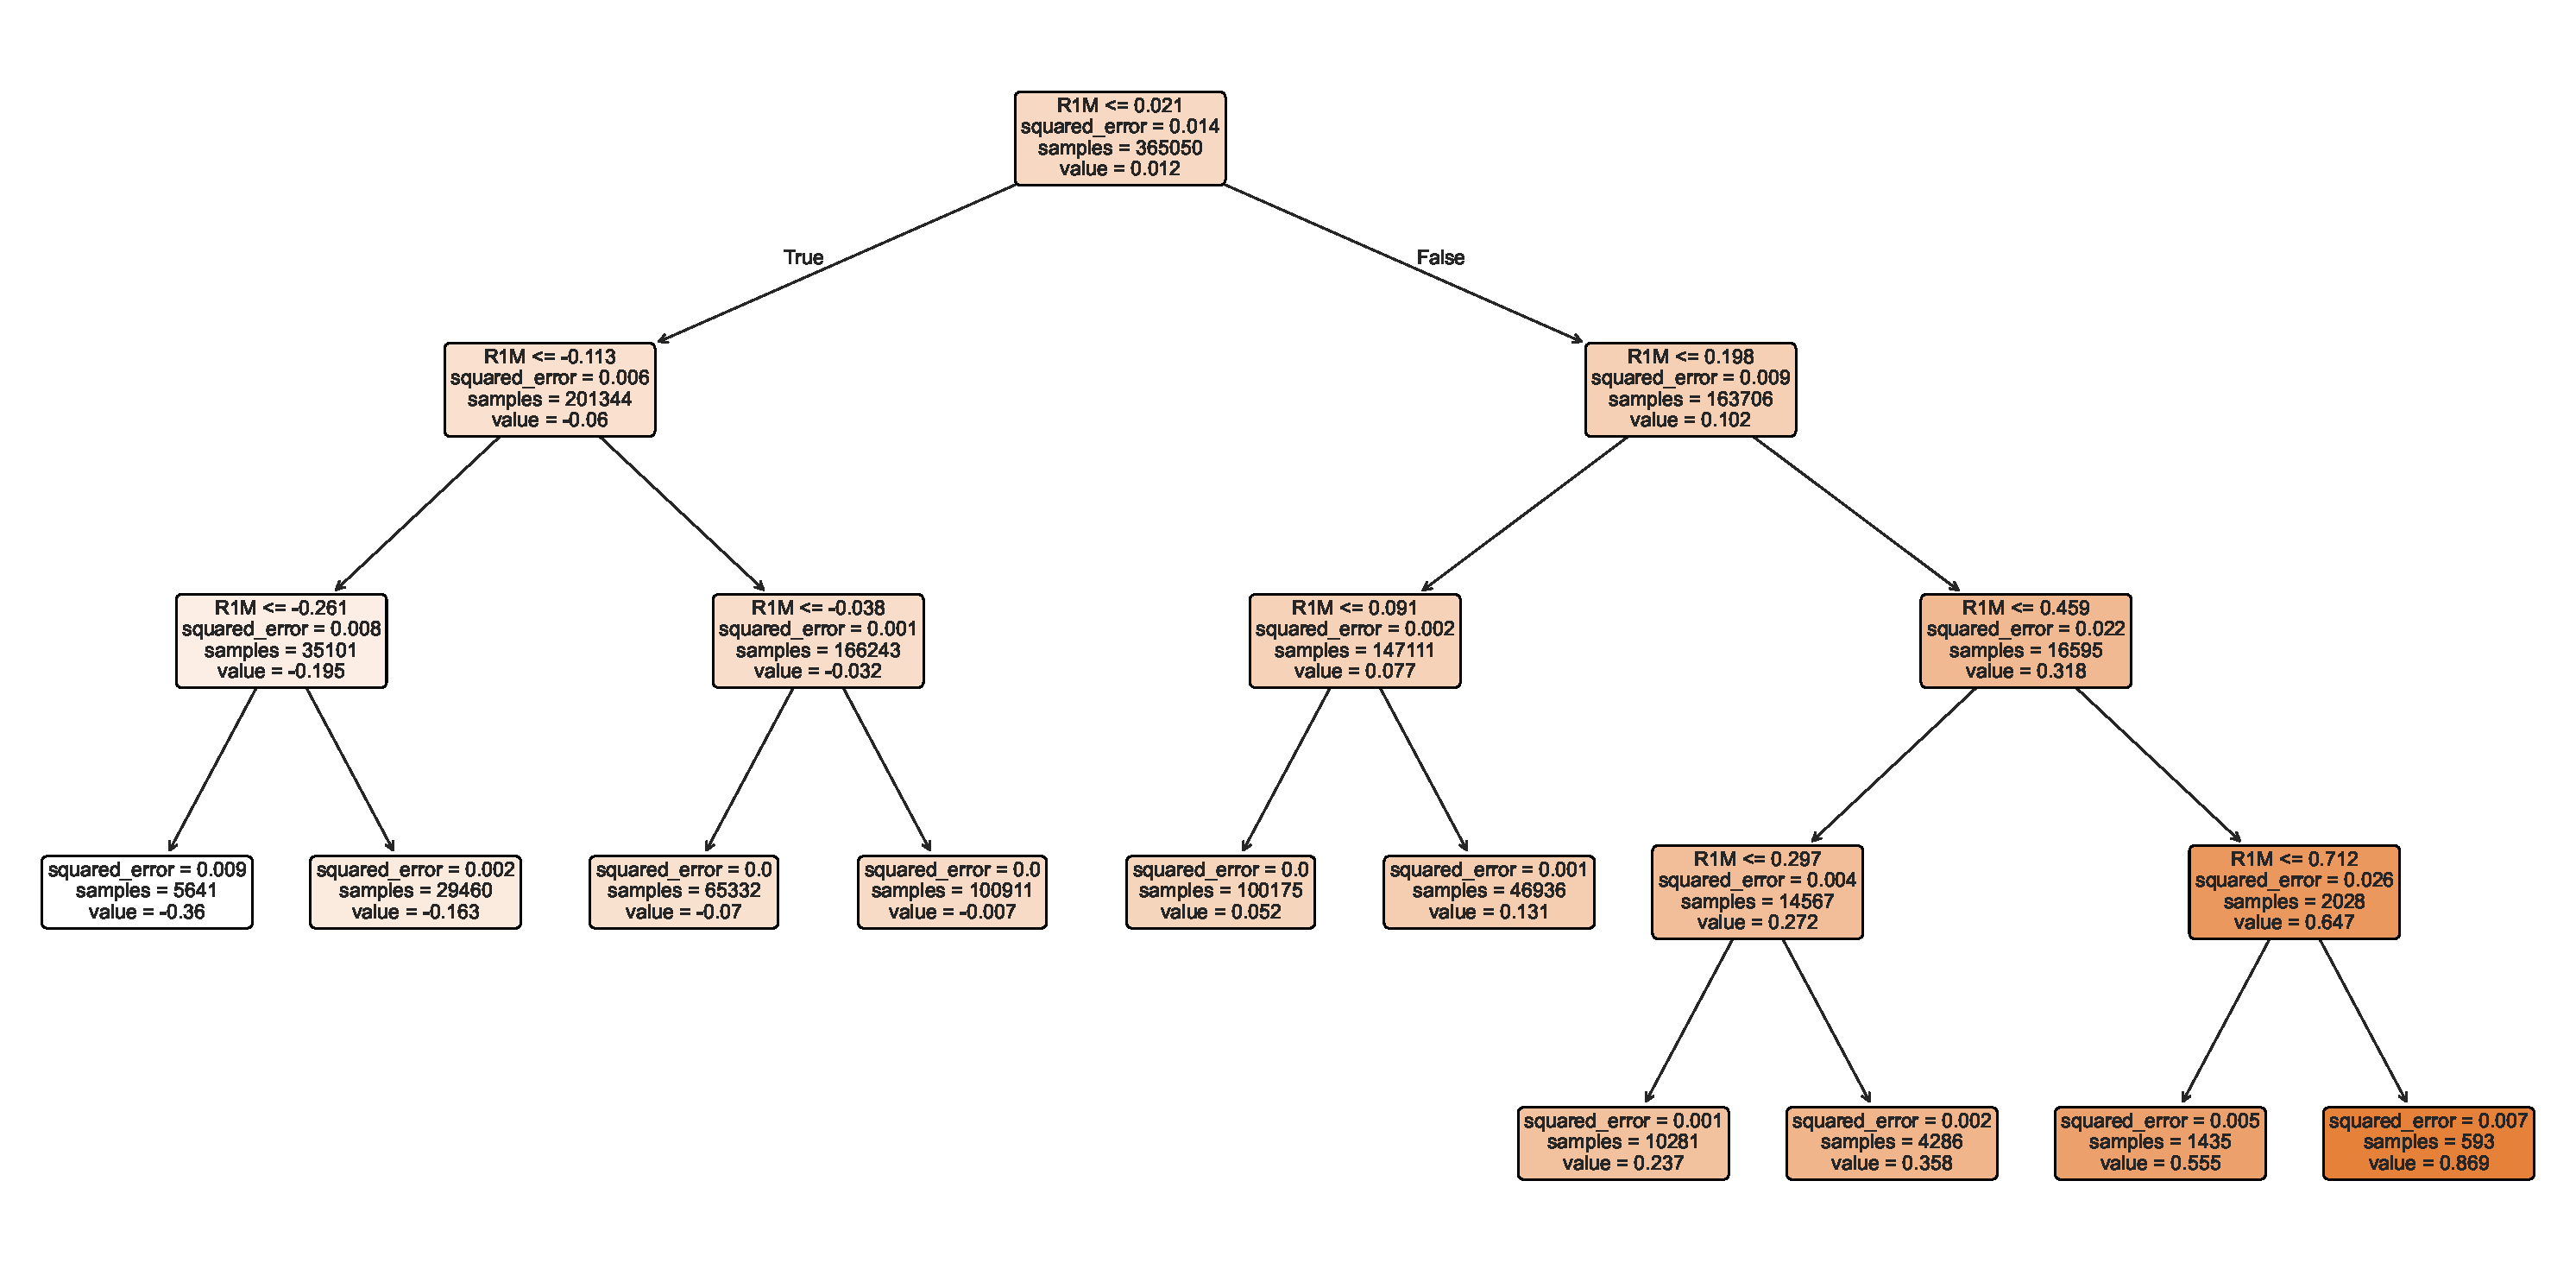
\includegraphics[width=0.7\linewidth]{files/65ecccb28beed48f15d9b3bdc6c3be99.pdf}}
\label{fig-first_tree}
\end{figure}

\begin{verbatim}
# Test (prediction) on the first six instances of the sample
fit_tree.predict(data_ml_clean[features].iloc[0:6])
\end{verbatim}

\begin{verbatim}
array([-0.16315559, -0.00704315,  0.05201558,  0.35764455, -0.00704315,
       -0.06951258])
\end{verbatim}

Given the figure, we immediately conclude that these first six instances all belong to the second cluster (starting from the left).

As a verification of the first splits, we plot the smoothed average of future returns, conditionally on market capitalization, price-to-book ratio and trading volume.

\begin{figure}[!htbp]
\centering
\begin{verbatim}
fig, ax = plt.subplots(figsize=(8, 6))

# Smoothed average of 1-month future returns, conditionally on different predictors
sns.regplot(data=data_ml, x='size_avg_252d', y='R1M', 
            scatter=False, lowess=True, label='Market Cap', ax=ax)
sns.regplot(data=data_ml, x='PB', y='R1M', 
            scatter=False, lowess=True, label='Price-to-Book', ax=ax)
sns.regplot(data=data_ml, x='ADV_TradedST', y='R1M', 
            scatter=False, lowess=True, label='Volume', ax=ax)

ax.set_xlabel('Predictor')
ax.legend(title='Characteristic')
plt.tight_layout()
plt.show()
\end{verbatim}
\caption[]{Average of 1-month future returns, conditionally on market capitalization, price-to-book and volume scores.

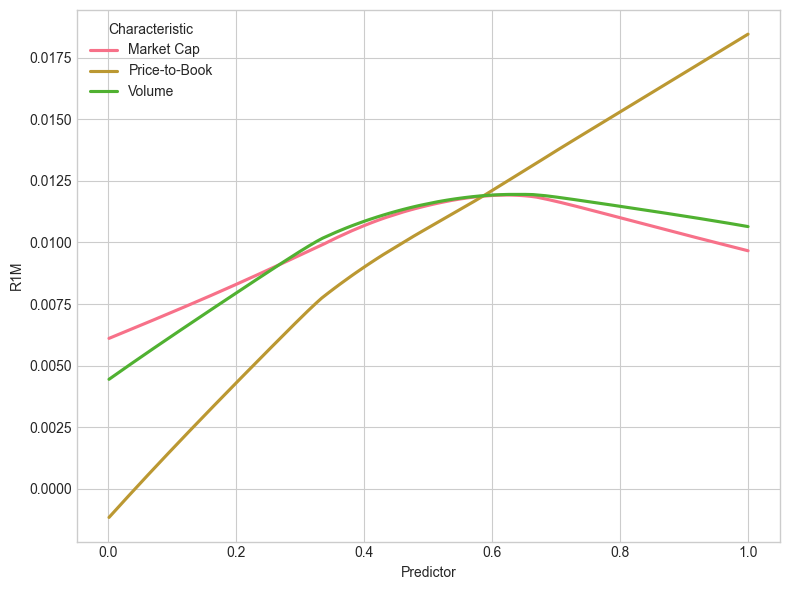
\includegraphics[width=0.7\linewidth]{files/427982a37bbda4b3d0508876d910456a.png}}
\label{fig-tree_cond}
\end{figure}

The graph shows the relevance of clusters based on market capitalizations and price-to-book ratios. For low score values of these two features, the average return is high (close to +4\% on a monthly basis on the left of the curves). The pattern is more pronounced compared to volume for instance.

Finally, we assess the predictive quality of a single tree on the testing set (the tree is grown on the training set). We use a deeper tree, with a maximum depth of five.

\begin{verbatim}
# Prepare training and testing data
training_sample = data_ml_clean[data_ml['date'] <= separation_date]
testing_sample = data_ml_clean[data_ml['date'] > separation_date]  # Prepare training and testing data
X_train = training_sample[features]
y_train = training_sample['R1M']
X_test = testing_sample[features]
y_test = testing_sample['R1M']

fit_tree2 = DecisionTreeRegressor(
    min_samples_leaf=1500,   # Min nb of obs required in each terminal node (leaf)
    min_samples_split=4000,  # Min nb of obs required to continue splitting
    ccp_alpha=0.0001,        # Complexity parameter: smaller = more leaves
    max_depth=5              # Maximum depth (i.e. tree levels)
)
fit_tree2.fit(X_train, y_train)

# Predictions
predictions = fit_tree2.predict(X_test)

# MSE
mse = np.round(np.mean((predictions - y_test) ** 2), 5)
print(f"MSE: {mse}")

# Hit ratio
hit_ratio = np.round(np.mean(predictions * y_test > 0), 5)
print(f"Hit ratio: {hit_ratio}")
\end{verbatim}

\begin{verbatim}
MSE: 0.00911
Hit ratio: 0.60256
\end{verbatim}

The mean squared error is usually hard to interpret. It's not easy to map an error on returns into the impact on investment decisions. The hit ratio is a more intuitive indicator because it evaluates the proportion of correct guesses (and hence profitable investments). Obviously, it is not perfect: 55\% of small gains can be mitigated by 45\% of large losses. Nonetheless, it is a popular metric and moreover it corresponds to the usual accuracy measure often computed in binary classification exercises. Here, an accuracy around 0.52 is satisfactory. Even if any number above 50\% may seem valuable, it must not be forgotten that transaction costs will curtail benefits. Hence, the benchmark threshold is probably at least at 52\%.

\subsubsection{Random forests}

While trees give intuitive representations of relationships between $\mathbf{Y}$ and $\mathbf{X}$, they can be improved via the simple idea of ensembles in which predicting tools are \textit{combined} (this topic of \textbf{model aggregation} is discussed both more generally and in more details in Chapter \href{/chap-14-ensemble}{Ensemble models}).

\paragraph{Principle}

Most of the time, when having several modelling options at hand, it is not obvious upfront which individual model is the best, hence a combination seems a reasonable path towards the diversification of prediction errors (when they are not too correlated). Some theoretical foundations of model diversification were laid out in \cite{schapire1990strength}.

More practical considerations were proposed later in \cite{ho1995random} and more importantly in \cite{breiman2001random} which is the major reference for random forests. Bagging is successfully used in \cite{yin2020equity} to aggregate equity forecasts. There are two ways to create multiple predictors from simple trees, and random forests combine both:

\begin{itemize}
\item first, the model can be trained on similar yet different datasets. One way to achieve this is via bootstrap: the instances are resampled with or without replacement (for each individual tree), yielding new training data each time a new tree is built.
\item second, the data can be altered by curtailing the number of predictors. Alternative models are built based on different sets of features. The user chooses how many features to retain and then the algorithm selects these features randomly at each try.
\end{itemize}

Hence, it becomes simple to grow many different trees and the ensemble is simply a \textbf{weighted combination} of all trees. Usually, equal weights are used, which is an agnostic and robust choice. We illustrate the idea of simple combinations (also referred to as bagging) in Figure~\ref{fig-RF} below. The terminal prediction is simply the mean of all intermediate predictions.

\begin{figure}[!htbp]
\centering
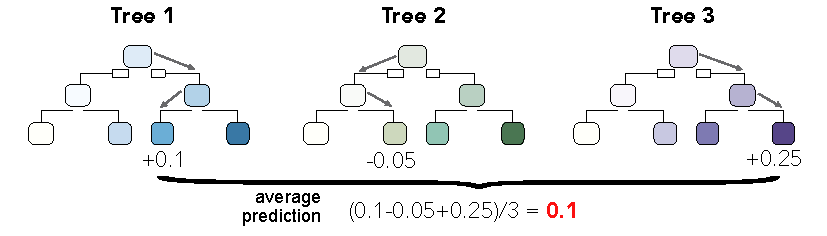
\includegraphics[width=0.7\linewidth]{files/tree_RF-7de0e11affee3e4d1f8cf3982d848f3d.pdf}
\caption[]{Diagram of a simple random forest.}
\label{fig-RF}
\end{figure}

Random forests, because they are built on the idea of bootstrapping, are more efficient than simple trees. They are used by \cite{ballings2015evaluating}, \cite{patel2015predicting}, \cite{krauss2017deep}, and \cite{huck2019large} and they are shown to perform very well in these papers. The original theoretical properties of random forests are demonstrated in \cite{breiman2001random} for classification trees. In classification exercises, the decision is taken by a vote: each tree votes for a particular class and the class with the most votes wins (with possible random picks in case of ties). \cite{breiman2001random} defines the margin function as

\begin{equation}
mg=M^{-1}\sum_{m=1}^M1_{\{h_m(\textbf{x})=y\}}-\max_{j\neq y}\left(M^{-1}\sum_{m=1}^M1_{\{h_m(\textbf{x})=j\}}\right),
\end{equation}

where the left part is the average number of votes based on the $M$ trees $h_m$ for the correct class (the models $h_m$ based on $\textbf{x}$ matches the data value $y$). The right part is the maximum average for any other class. The margin reflects the confidence that the aggregate forest will classify properly. The generalization error is the probability that $mg$ is strictly negative. \cite{breiman2001random} shows that the inaccuracy of the aggregation (as measured by generalization error) is bounded by $\bar{\rho}(1 -s^2)/s^2$, where

\begin{itemize}
\item $s$ is the strength (average quality\footnote{The strength is measured as the average margin, i.e. the average of $mg$ when there is only one tree.}) of the individual classifiers and
\item $\bar{\rho}$ is the average correlation between the learners.
\end{itemize}

Notably, \cite{breiman2001random} also shows that as the number of trees grows to infinity, the inaccuracy converges to some finite number which explains why random forests are not prone to overfitting.

While the original paper of \cite{breiman2001random} is dedicated to classification models, many articles have since then tackled the problem of regression trees. We refer the interested reader to \cite{biau2012analysis} and \cite{scornet2015consistency}. Finally, further results on classifying ensembles can be obtained in \cite{biau2008consistency} and we mention the short survey paper by \cite{denil2014narrowing} which sums up recent results in this field.

\paragraph{Code and results}

Several implementations of random forests exist. For simplicity, we choose to work with the scikit-learn library, but another choice could be the one developed by h2o, which is a highly efficient meta-environment for machine learning (coded in Java).

The syntax of RandomForestRegressor follows that of many ML libraries. The full list of options for some random forest implementations is prohibitively large.\footnote{See, e.g., \href{http://docs.h2o.ai/h2o/latest-stable/h2o-r/docs/reference/h2o.randomForest.html}{http://docs.h2o.ai/h2o/latest-stable/h2o-r/docs/reference/h2o.randomForest.html}} Below, we train a model and exhibit the predictions for the first 5 instances of the testing sample.

\begin{verbatim}
from sklearn.ensemble import RandomForestRegressor
np.random.seed(42)  # Sets the random seed

X_train = training_sample[features]
y_train = training_sample['R1M']
X_test = testing_sample[features]
y_test = testing_sample['R1M']

fit_RF = RandomForestRegressor(
    n_estimators=40,         # Nb of random trees
    max_samples=10000,       # Size of (random) sample for each tree
    bootstrap=True,          # Sampling with replacement (set False for without)
    min_samples_leaf=250,    # Minimum size of terminal cluster
    max_features=30,         # Nb of predictive variables for each tree
    random_state=42
)
fit_RF.fit(X_train, y_train)

# Prediction over the first 5 test instances
fit_RF.predict(X_test.iloc[0:5])
\end{verbatim}

\begin{verbatim}
array([ 0.05552201,  0.02574694, -0.0067237 ,  0.03020125,  0.03718925])
\end{verbatim}

One first comment is that each instance has its own prediction, which contrasts with the outcome of simple tree-based outcomes. Combining many trees leads to tailored forecasts. Note that the second line of the chunk freezes the random number generation. Indeed, random forests are by construction contingent on the arbitrary combinations of instances and features that are chosen to build the individual learners.

In the above example, each individual learner (tree) is built on 10,000 randomly chosen instances (without replacement) and each terminal leaf (cluster) must comprise at least 240 elements (observations). In total, 40 trees are aggregated and each tree is constructed based on 30 randomly chosen predictors (out of the whole set of features).

Unlike for simple trees, it is not possible to simply illustrate the outcome of the learning process (though solutions exist, see Section~\ref{surr}). It could be possible to extract all 40 trees, but a synthetic visualization is out-of-reach. A simplified view can be obtained via variable importance, as is discussed in Section~\ref{variable-importance}.

Finally, we can assess the accuracy of the model.

\begin{verbatim}
predictions_RF = fit_RF.predict(X_test)

# MSE
mse_RF = np.round(np.mean((predictions_RF - y_test) ** 2), 5)
print(f"MSE: {mse_RF}")

# Hit ratio
hit_ratio_RF = np.round(np.mean(predictions_RF * y_test > 0), 5)
print(f"Hit ratio: {hit_ratio_RF}")
\end{verbatim}

\begin{verbatim}
MSE: 0.00888
Hit ratio: 0.61025
\end{verbatim}

The MSE is smaller than 4\% and the hit ratio is close to 54\%, which is reasonably above both 50\% and 52\% thresholds.

Let's see if we can improve the hit ratio by resorting to a classification exercise. We start by training the model on a new formula (the label is R1M\_C).

\begin{verbatim}
from sklearn.ensemble import RandomForestClassifier

# For classification, we use the categorical label R1M_C
y_train_C = training_sample['R1M_C']
y_test_C = testing_sample['R1M_C']

fit_RF_C = RandomForestClassifier(
    n_estimators=40,         # Nb of random trees
    max_samples=20000,       # Size of (random) sample for each tree
    bootstrap=True,          # Sampling with replacement
    min_samples_leaf=250,    # Minimum size of terminal cluster
    max_features=30,         # Nb of predictive variables for each tree
    random_state=42
)
fit_RF_C.fit(X_train, y_train_C)
\end{verbatim}

\begin{verbatim}
RandomForestClassifier(max_features=30, max_samples=20000, min_samples_leaf=250,
                       n_estimators=40, random_state=42)
\end{verbatim}

We can then assess the proportion of correct (binary) guesses.

\begin{verbatim}
# Hit ratio for classification
predictions_RF_C = fit_RF_C.predict(X_test)
hit_ratio_C = np.round(np.mean(predictions_RF_C == y_test_C), 5)
print(f"Hit ratio: {hit_ratio_C}")
\end{verbatim}

\begin{verbatim}
Hit ratio: 0.64274
\end{verbatim}

The accuracy is disappointing. There are two potential explanations for this (beyond the possibility of very different patterns in the training and testing sets). The first one is the sample size, which may be too small. The original training set has more than 200,000 observations, hence we retain only one in 10 in the above training specification. We are thus probably sidelining relevant information and the cost can be heavy. The second reason is the number of predictors, which is set to 30, i.e., one third of the total at our disposal. Unfortunately, this leaves room for the algorithm to pick less pertinent predictors. The default numbers of predictors chosen by the routines are $\sqrt{p}$ and $p/3$ for classification and regression tasks, respectively. Here $p$ is the total number of features.

\subsubsection{Boosted trees: Adaboost}\label{sec_adaboost}

The idea of boosting is slightly more advanced compared to agnostic aggregation. In random forest, we hope that the diversification through many trees will improve the overall quality of the model. In boosting, it is sought to iteratively improve the model whenever a new tree is added. There are many ways to boost learning and we present two that can easily be implemented with trees. The first one (Adaboost, for adaptive boosting) improves the learning process by progressively focusing on the instances that yield the largest errors. The second one (xgboost) is a flexible algorithm in which each new tree is only focused on the minimization of the training sample loss.

\paragraph{Methodology}

The origins of adaboost go back to \cite{freund1997decision} and \cite{freund1996experiments}, and for the sake of completeness, we also mention the book dedicated to boosting by \cite{schapire2012boosting}. Extensions of these ideas are proposed in \cite{friedman2000additive} (the so-called real Adaboost algorithm) and in \cite{drucker1997improving} (for regression analysis). Theoretical treatments were derived by \cite{breiman2004population}.

We start by directly stating the general structure of the algorithm:

\begin{itemize}
\item set equal weights $w_i=I^{ -1}$;
\item For $m=1,\dots,M$ do:
\end{itemize}

\begin{enumerate}
\item Find a learner $l_m$ that minimizes the weighted loss $\sum_{i=1}^Iw_iL(l_m(\textbf{x}_i),\textbf{y}_i)$;
\item Compute a learner weight

\begin{equation}
a_m=f_a(\textbf{w},l_m(\textbf{x}),\textbf{y});
\end{equation}


\item Update the instance weights

\begin{equation}
w_i \leftarrow w_ie^{f_w(l_m(\textbf{x}_i), \textbf{y}_i)};
\end{equation}


\item Normalize the $w_i$ to sum to one.
\end{enumerate}

\begin{itemize}
\item The output for instance $\textbf{x}_i$ is a simple function of $\sum_{m=1}^M a_ml_m(\textbf{x}_i)$,

\begin{equation}
\tilde{y}_i=f_y\left(\sum_{m=1}^M a_ml_m(\textbf{x}_i) \right).
\end{equation}
\end{itemize}

Let us comment on the steps of the algorithm. The formulation holds for many variations of Adaboost and we will specify the functions $f_a$ and $f_w$ below.

\begin{enumerate}
\item The first step seeks to find a learner (tree) $l_m$ that minimizes a weighted loss. Here the base loss function $L$ essentially depends on the task (regression versus classification).
\item The second and third steps are the most interesting because they are the heart of Adaboost: they define the way the algorithm adapts sequentially. Because the purpose is to aggregate models, a more sophisticated approach compared to uniform weights for learners is a tailored weight for each learner. A natural property (for $f_a$) should be that a learner that yields a smaller error should have a larger weight because it is more accurate.
\item The third step is to change the weights of observations. In this case, because the model aims at improving the learning process, $f_w$ is constructed to give more weight on observations for which the current model does not do a good job (i.e., generates the largest errors). Hence, the next learner will be incentivized to pay more attention to these pathological cases.
\item The third step is a simple scaling procedure.
\end{enumerate}

In Table Section~\ref{sec_adaboost}, we detail two examples of weighting functions used in the literature. For the original Adaboost (\cite{freund1996experiments}, \cite{freund1997decision}), the label is binary with values +1 and -1 only. The second example stems from \cite{drucker1997improving} and is dedicated to regression analysis (with real-valued label). The interested reader can have a look at other possibilities in \cite{schapire2003boosting} and \cite{ridgeway1999boosting}.

\bigskip\noindent
\begin{tabular}{p{\dimexpr 0.333\linewidth-2\tabcolsep}p{\dimexpr 0.333\linewidth-2\tabcolsep}p{\dimexpr 0.333\linewidth-2\tabcolsep}}
\toprule
 & Bin. classif. (orig. Adaboost) & Regression (Drucker (1997)) \\
\hline
Individual error & $\epsilon_i=\textbf{1}_{\left\{y_i\neq l_m(\textbf{x}_i) \right\}}$ & \${\textbackslash}epsilon\_i={\textbackslash}frac\{ \\
Weight of learner via $f_a$ & $f_a=\log\left(\frac{1 -\epsilon}{\epsilon} \right)$,with  $\epsilon=I^{ -1}\sum_{i=1}^Iw_i \epsilon_i$ & $f_a=\log\left(\frac{1 -\epsilon}{\epsilon} \right)$,with  $\epsilon=I^{ -1}\sum_{i=1}^Iw_i \epsilon_i$ \\
Weight of instances via $f_w(i)$ & $f_w=f_a\epsilon_i$ & $f_w=f_a\epsilon_i$ \\
Output function via $f_y$ & $f_y(x) = \text{sign}(x)$ & weighted median of predictions \\
\bottomrule
\end{tabular}

\bigskip

Table: Examples of functions for Adaboost-like algorithms.

Let us comment on the original Adaboost specification. The basic error term $\epsilon_i=\textbf{1}_{\left\{y_i\neq l_m(\textbf{x}_i) \right\}}$ is a dummy number indicating if the prediction is correct (we recall only two values are possible, +1 and -1). The average error $\epsilon\in [0,1]$ is simply a weighted average of individual errors and the weight of the $m^{th}$ learner defined in Equation @ref(eq:adaboostam) is given by $a_m=\log\left(\frac{1 -\epsilon}{\epsilon} \right)$. The function $x\mapsto \log((1 -x)x^{ -1})$ decreases on $[0,1]$ and switches sign (from positive to negative) at $x=1/2$. Hence, when the average error is small, the learner has a large positive weight, but when the error becomes large, the learner can even obtain a negative weight. Indeed, the threshold $\epsilon>1/2$ indicated that the learner is wrong more than 50\% of the time. Obviously, this indicates a problem and the learner should even be discarded.

The change in instance weights follows a similar logic. The new weight is proportional to $w_i\left(\frac{1 -\epsilon}{\epsilon} \right)^{\epsilon_i}$. If the prediction is right and $\epsilon_i=0$, the weight is unchanged. If the prediction is wrong and $\epsilon_i=1$, the weight is adjusted depending on the aggregate error $\epsilon$. If the error is small and the learner efficient ($\epsilon<1/2$), then $(1 -\epsilon)/\epsilon>1$ and the weight of the instance increases. This means that for the next round, the learner will have to focus more on instance $i$.

Lastly, the final prediction of the model corresponds to the sign of the weighted sums of individual predictions: if the sum is positive, the model will predict +1 and it will yield -1 otherwise.\footnote{The Real Adaboost of \cite{friedman2000additive} has a different output: the probability of belonging to a particular class.} The odds of a zero sum are negligible. In the case of numerical labels, the process is slightly more complicated and we refer to Section 3, step 8 of \cite{drucker1997improving} for more details on how to proceed.

We end this presentation with one word on instance weighting. There are two ways to deal with this topic. The first one works at the level of the loss functions. For regression trees, Equation @ref(eq:node) would naturally generalize to
\begin{equation}
V^{(k)}_N(c^{(k)}, \textbf{w})= \sum_{x_i^{(k)}<c^{(k)}}w_i\left(y_i-m_N^{k,-}(c^{(k)}) \right)^2 + \sum_{x_i^{(k)}>c^{(k)}}w_i\left(y_i-m_N^{k,+}(c^{(k)}) \right)^2,
\end{equation}

and hence an instance with a large weight $w_i$ would contribute more to the dispersion of its cluster. For classification objectives, the alteration is more complex and we refer to \cite{ting2002instance} for one example of an instance-weighted tree-growing algorithm. The idea is closely linked to the alteration of the misclassification risk via a loss matrix (see Section 9.2.4 in \cite{friedman2009elements}).

The second way to enforce instance weighting is via random sampling. If instances have weights $w_i$, then the training of learners can be performed over a sample that is randomly extracted with distribution equal to $w_i$. In this case, an instance with a larger weight will have more chances to be represented in the training sample. The original adaboost algorithm relies on this method.

\paragraph{Illustration}

Below, we test an implementation of the original Adaboost classifier. As such, we work with the R1M\_C variable and change the model formula. The computational cost of Adaboost is high on large datasets, thus we work with a smaller sample and we only impose three iterations.

\begin{verbatim}
X_train_ada = training_sample[features]
y_train_ada = training_sample['R1M_C']

# Adaboost classifier
fit_adaboost_C = AdaBoostClassifier(
    estimator=DecisionTreeClassifier(max_depth=2),  # Base estimator (decision stump)
    n_estimators=3,                                  # Number of trees
    random_state=42
)
fit_adaboost_C.fit(X_train_ada, y_train_ada)
\end{verbatim}

\begin{verbatim}
AdaBoostClassifier(estimator=DecisionTreeClassifier(max_depth=2),
                   n_estimators=3, random_state=42)
\end{verbatim}

Finally, we evaluate the performance of the classifier.

\begin{verbatim}
# Hit ratio
predictions_ada = fit_adaboost_C.predict(testing_sample[features])
hit_ratio_ada = np.mean(testing_sample['R1M_C'] == predictions_ada)
print(f"Hit ratio: {hit_ratio_ada}")
\end{verbatim}

\begin{verbatim}
Hit ratio: 0.6249692829409741
\end{verbatim}

The accuracy (as evaluated by the hit ratio) is clearly not satisfactory. One reason for this may be the restrictions we enforced for the training (smaller sample and only three trees).

\subsubsection{Boosted trees: extreme gradient boosting}

The ideas behind \textbf{tree boosting} were popularized, among others, by \cite{mason2000boosting}, \cite{friedman2001greedy}, and \cite{friedman2002stochastic}. In this case, the combination of learners (prediction tools) is not agnostic as in random forest, but adapted (or optimized) at the learner level. At each step $s$, the sum of models $M_S=\sum_{s=1}^{S -1}m_s+m_S$ is such that the last learner $m_S$ was precisely designed to reduce the loss of $M_S$ on the training sample.

Below, we follow closely the original work of \cite{chen2016xgboost} because their algorithm yields incredibly accurate predictions and also because it is highly customizable. It is their implementation that we use in our empirical section. The other popular alternative is lightgbm (see \cite{ke2017lightgbm}). What XGBoost seeks to minimize is the objective
\begin{equation}
O=\underbrace{\sum_{i=1}^I \text{loss}(y_i,\tilde{y}_i)}_{\text{error term}} \quad + \underbrace{\sum_{j=1}^J\Omega(T_j)}_{\text{regularization term}}.
\end{equation}
The first term (over all instances) measures the distance between the true label and the output from the model. The second term (over all trees) penalizes models that are too complex.

For simplicity, we propose the full derivation with the simplest loss function $\text{loss}(y,\tilde{y})=(y -\tilde{y})^2$, so that:
\begin{equation}
O=\sum_{i=1}^I \left(y_i-m_{J-1}(\mathbf{x}_i)-T_J(\mathbf{x}_i)\right)^2+ \sum_{j=1}^J\Omega(T_j).
\end{equation}

\paragraph{Managing loss}

Let us assume that we have already built all trees $T_{j}$ up to $j=1,\dots,J -1$ (and hence model $M_{J -1}$): how to choose tree $T_J$ optimally? We rewrite
\begin{equation}
\begin{aligned}
O&=\sum_{i=1}^I \left(y_i-m_{J-1}(\mathbf{x}_i)-T_J(\mathbf{x}_i)\right)^2+ \sum_{j=1}^J\Omega(T_j) \\
&=\sum_{i=1}^I\left\{y_i^2+m_{J-1}(\mathbf{x}_i)^2+T_J(\mathbf{x}_i)^2 \right\} + \sum_{j=1}^{J-1}\Omega(T_j)+\Omega(T_J) \quad \text{(squared terms + penalization)}\\
& \quad -2 \sum_{i=1}^I\left\{y_im_{J-1}(\mathbf{x}_i)+y_iT_J(\mathbf{x}_i)-m_{J-1}(\mathbf{x}_i) T_J(\mathbf{x}_i))\right\}\quad \text{(cross terms)} \\
&= \sum_{i=1}^I\left\{-2 y_iT_J(\mathbf{x}_i)+2m_{J-1}(\mathbf{x}_i) T_J(\mathbf{x}_i))+T_J(\mathbf{x}_i)^2 \right\} +\Omega(T_J) + c
\end{aligned}
\end{equation}
All terms known at step $J$ (i.e., indexed by $J -1$) vanish because they do not enter the optimization scheme. They are embedded in the constant $c$.

Things are fairly simple with quadratic loss. For more complicated loss functions, Taylor expansions are used (see the original paper).

\paragraph{Penalization}

In order to go any further, we need to specify the way the penalization works. For a given tree $T$, we specify its structure by $T(x)=w_{q(x)}$, where $w$ is the output value of some leaf and $q(\cdot)$ is the function that maps an input to its final leaf. This encoding is illustrated in \href{\#fig:-ree\_q}{}. The function $q$ indicates the path, while the vector $\textbf{w}=w_i$ codes the terminal leaf values.

\begin{figure}[!htbp]
\centering
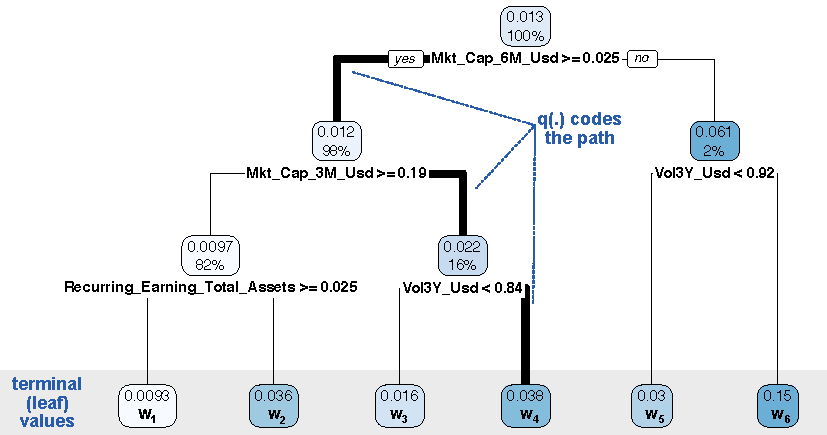
\includegraphics[width=0.7\linewidth]{files/tree_q-81952e984ffd8cf175f6d2e60bb2a1b3.pdf}
\caption[]{Diagram of the coding of a single boosted tree.}
\label{fig-tree_q}
\end{figure}

We write $l=1,\dots,L$ for the indices of the leaves of the tree. In XGBoost, complexity is defined as:
\begin{equation}
\Omega(T)=\gamma L+\frac{\lambda}{2}\sum_{l=1}^Lw_l^2,
\end{equation}
where

\begin{itemize}
\item the first term penalizes the \textbf{total number of leaves};
\item the second term penalizes the \textbf{magnitude of output values} (this helps reduce variance).
\end{itemize}

The first penalization term reduces the depth of the tree, while the second shrinks the size of the adjustments that will come from the latest tree.

\paragraph{Aggregation}

We aggregate both sections of the objective (loss and penalization). We write $I_l$ for the set of the indices of the instances belonging to leaf $l$. Then,\newline
\begin{equation}
\begin{aligned}
O&= 2\sum_{i=1}^I\left\{ -y_iT_J(\mathbf{x}_i)+m_{J-1}(\mathbf{x}_i) T_J(\mathbf{x}_i))+\frac{T_J(\mathbf{x}_i)^2}{2} \right\} + \gamma L+\frac{\lambda}{2}\sum_{l=1}^Lw_l^2 \\
&=2\sum_{i=1}^I\left\{- y_iw_{q(\mathbf{x}_i)}+m_{J-1}(\mathbf{x}_i)w_{q(\mathbf{x}_i)})+\frac{w_{q(\mathbf{x}_i)}^2}{2} \right\} + \gamma L+\frac{\lambda}{2}\sum_{l=1}^Lw_l^2 \\
&=2 \sum_{l=1}^L \left(w_l\sum_{i\in I_l}(-y_i +m_{J-1}(\mathbf{x}_i))+ \frac{w_l^2}{2}\sum_{i\in I_l}\left(1+\frac{\lambda}{2}\right)\right)+ \gamma L
\end{aligned}
\end{equation}
The function is of the form $aw_l+\frac{b}{2}w_l^2$, which has minimum values $-\frac{a^2}{2b}$ at point $w_l= -a/b$. Thus, writing $\#(\cdot)$ for the cardinal function that counts the number of items in a set,
\begin{equation}
\begin{aligned}
\mathbf{\rightarrow} \quad w^*_l&=\frac{\sum_{i\in I_l}(y_i -m_{J-1}(\mathbf{x}_i))}{\left(1+\frac{\lambda}{2}\right)\#\{i\in I_l\}}, \text{ so that} \\
O_L(q)&=-\frac{1}{2}\sum_{l=1}^L \frac{\left(\sum_{i\in I_l}(y_i -m_{J-1}(\mathbf{x}_i))\right)^2}{\left(1+\frac{\lambda}{2}\right)\#\{i\in I_l\}}+\gamma L, \nonumber
\end{aligned}
\end{equation}
where we added the dependence of the objective both in $q$ (structure of tree) and $L$ (number of leaves). Indeed, the meta-shape of the tree remains to be determined.

\paragraph{Tree structure}

Final problem: the \textbf{tree structure}! Let us take a step back. In the construction of a simple regression tree, the output value at each node is equal to the average value of the label within the node (or cluster). When adding a new tree in order to reduce the loss, the node values must be computed completely differently, which is the purpose of Equation @ref(eq:xgbweight).

Nonetheless, the growing of the iterative trees follows similar lines as simple trees. Features must be tested in order to pick the one that minimizes the objective for each given split. The final question is then: what's the best depth and when to stop growing the tree? The method is to

\begin{itemize}
\item proceed node-by-node;
\item for each node, look at whether a split is useful (in terms of objective) or not:

\begin{equation}
\text{Gain}=\frac{1}{2}\left(\text{Gain}_L+\text{Gain}_R-\text{Gain}_O \right)-\gamma
\end{equation}


\item each gain is computed with respect to the instances in each bucket (cluster):

\begin{equation}
\text{Gain}_\mathcal{X}= \frac{\left(\sum_{i\in I_\mathcal{X}}(y_i -m_{J-1}(\mathbf{x}_i))\right)^2}{\left(1+\frac{\lambda}{2}\right)\#\{i\in I_\mathcal{X}\}},
\end{equation}


where $I_\mathcal{X}$ is the set of instances within cluster $\mathcal{X}$.
\end{itemize}

$\text{Gain}_O$ is the original gain (no split) and $\text{Gain}_L$ and $\text{Gain}_R$ are the gains of the left and right clusters, respectively. One word about the $-\gamma$ adjustment in the above formula: there is one unit of new leaves (two new minus one old)! This makes a one leaf difference; hence $\Delta L =1$ and the penalization intensity for each new leaf is equal to $\gamma$.

Lastly, we underline the fact that XGBoost also applies a \textbf{learning rate}: each new tree is scaled by a factor $\eta$, with $\eta \in (0,1]$. After each step of boosting the new tree $T_J$ sees its values discounted by multiplying them by $\eta$. This is very useful because a pure aggregation of 100 optimized trees is the best way to overfit the training sample.

\paragraph{Extensions}\label{sec_boostext}

Several additional features are available to further prevent boosted trees to overfit. Indeed, given a sufficiently large number of trees, the aggregation is able to match the training sample very well, but may fail to generalize well out-of-sample.

Following the pioneering work of \cite{srivastava2014dropout}, the DART (Dropout for Additive Regression Trees) model was proposed by \cite{rashmi2015dart}. The idea is to omit a specified number of trees during training. The trees that are removed from the model are chosen randomly. The full specifications can be found at \href{https://xgboost.readthedocs.io/en/latest/tutorials/dart.html}{https://xgboost.readthedocs.io/en/latest/tutorials/dart.html} and we use a 10\% dropout in the first example below.

Monotonicity constraints are another element that is featured both in xgboost and lightgbm. Sometimes, it is expected that one particular feature has a monotonic impact on the label. For instance, if one deeply believes in momentum, then past returns should have an increasing impact on future returns (in the cross-section of stocks).

Given the recursive nature of the splitting algorithm, it is possible to choose when to perform a split (according to a particular variable) and when not to. In Figure~\ref{fig-tree_monotonic}, we show how the algorithm proceeds. All splits are performed according to the same feature. For the first split, things are easy because it suffices to verify that the averages of each cluster are ranked in the right direction. Things are more complicated for the splits that occur below. Indeed, the average values set by all above splits matter as they give bounds for acceptable values for the future average values in lower splits. If a split violates these bounds, then it is overlooked and another variable will be chosen instead.

\begin{figure}[!htbp]
\centering
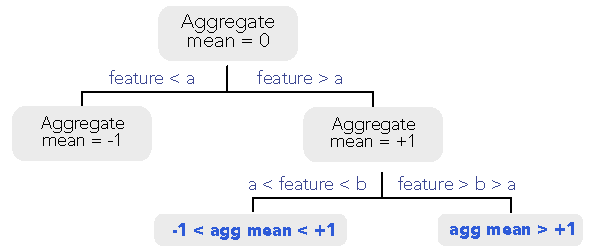
\includegraphics[width=0.7\linewidth]{files/tree_monotonic-4c4da3f09ed6577bf4c2f28bb91ee8c3.pdf}
\caption[]{Explanation of monotonic constraints.}
\label{fig-tree_monotonic}
\end{figure}

\paragraph{Code and results}\label{boostcode}

In this section, we train a model using the \textit{XGBoost} library. Other options include \textit{catboost}, \textit{gbm}, \textit{lightgbm}, and \textit{h2o}'s own version of boosted machines. Unlike many other packages, the XGBoost function requires a particular syntax and dedicated formats. The first step is thus to encapsulate the data accordingly.

Moreover, because training times can be long, we shorten the training sample as advocated in \cite{coqueret2019training}. We retain only the 40\% most extreme observations (in terms of label values: top 20\% and bottom 20\%) and work with the small subset of features. In all coding sections dedicated to boosted trees in this book, the models will be trained with only 7 features.

\begin{verbatim}
# Filter extreme values only (top 20% and bottom 20%)
q20 = training_sample['R1M'].quantile(0.2)
q80 = training_sample['R1M'].quantile(0.8)

train_extreme = training_sample[
    (training_sample['R1M'] < q20) | (training_sample['R1M'] > q80)
]

train_features_xgb = train_extreme[features].values  # Independent variables
train_label_xgb = train_extreme['R1M'].values        # Dependent variable

# XGB DMatrix format
train_matrix_xgb = xgb.DMatrix(data=train_features_xgb, label=train_label_xgb)
\end{verbatim}

The second (optional) step is to determine the monotonicity constraints that we want to impose. For simplicity, we will only enforce three constraints on

\begin{enumerate}
\item market capitalization (negative, because large firms have smaller returns under the size anomaly);
\item price-to-book ratio (negative, because overvalued firms also have smaller returns under the value anomaly);
\item past annual returns (positive, because winners outperform losers under the momentum anomaly).
\end{enumerate}

\begin{verbatim}
# Initialize the monotonicity constraints vector
mono_const = [0] * len(features)

# Set constraints (need to find indices in features list)
if 'size_avg_252d' in features:
    mono_const[features.index('size_avg_252d')] = -1  # Decreasing in market cap
if 'PB' in features:
    mono_const[features.index('PB')] = -1              # Decreasing in price-to-book
if 'mom_252' in features:
    mono_const[features.index('mom_252')] = 1      # Increasing in past return

# Convert to tuple format for xgboost
mono_const_tuple = tuple(mono_const)
\end{verbatim}

The third step is to train the model on the formatted training data. We include the monotonicity constraints and the DART feature (via \textit{rate\_drop}). Just like random forests, boosted trees can grow individual trees on subsets of the data: both row-wise (by selecting random instances) and column-wise (by keeping a smaller portion of predictors). These options are implemented below with the \textit{subsample} and \textit{colsample\_bytree} in the arguments of the function.

\begin{verbatim}
# XGBoost parameters
params = {
    'eta': 0.3,                          # Learning rate
    'objective': 'reg:squarederror',     # Objective function
    'max_depth': 4,                      # Maximum depth of trees
    'subsample': 0.6,                    # Train on random 60% of sample
    'colsample_bytree': 0.7,             # Train on random 70% of predictors
    'lambda': 1,                         # Penalisation of leaf values (reg_lambda)
    'gamma': 0.1,                        # Penalisation of number of leaves
    'monotone_constraints': mono_const_tuple,  # Monotonicity constraints
    'rate_drop': 0.1,                    # Drop rate for DART
    'verbosity': 0                       # No comment from the algo
}

# Train the model
fit_xgb = xgb.train(
    params=params,
    dtrain=train_matrix_xgb,
    num_boost_round=30                   # Number of trees used (rather low here)
)
\end{verbatim}

Finally, we evaluate the performance of the model. Note that before that, a proper formatting of the testing sample is required.

\begin{verbatim}
# Test sample => XGB format
xgb_test = xgb.DMatrix(testing_sample[features].values)

# Predictions
predictions_xgb = fit_xgb.predict(xgb_test)

# MSE
mse_xgb = np.mean((predictions_xgb - testing_sample['R1M'].values) ** 2)
print(f"MSE: {np.round(mse_xgb, 5)}")

# Hit ratio
hit_ratio_xgb = np.mean(predictions_xgb * testing_sample['R1M'].values > 0)
print(f"Hit ratio: {np.round(hit_ratio_xgb, 5)}")
\end{verbatim}

\begin{verbatim}
MSE: 0.00869
Hit ratio: 0.62207
\end{verbatim}

The performance is comparable to those observed for other predictive tools. As a final exercise, we show one implementation of a classification task under XGBoost. Only the label changes. In XGBoost, labels must be coded with integer number, starting at zero exactly.

\begin{verbatim}
# Filter for classification: extreme returns only
train_extreme_C = training_sample[
    (training_sample['R1M'] < q20) | (training_sample['R1M'] > q80)
]

# Create binary label (1 if R1M_C is True/positive class, 0 otherwise)
train_label_C = (train_extreme_C['R1M_C'] == True).astype(int).values

# XGB DMatrix format for classification
train_matrix_C = xgb.DMatrix(data=train_features_xgb, label=train_label_C)
\end{verbatim}

When working with categories, the loss function is usually the softmax function (see Section @ref(notations)).

\begin{verbatim}
# XGBoost classification parameters
params_C = {
    'eta': 0.8,                          # Learning rate
    'objective': 'multi:softmax',        # Objective function
    'num_class': 2,                      # Number of classes
    'max_depth': 4,                      # Maximum depth of trees
    'verbosity': 0                       # No warning message
}

# Train the classification model
fit_xgb_C = xgb.train(
    params=params_C,
    dtrain=train_matrix_C,
    num_boost_round=10                   # Number of trees used
)
\end{verbatim}

We can then proceed to the assessment of the quality of the model. We adjust the prediction to the value of the true label and count the proportion of accurate forecasts.

\begin{verbatim}
# Predictions
predictions_xgb_C = fit_xgb_C.predict(xgb_test)

# Convert testing labels to same format
test_labels_C = (testing_sample['R1M_C'] == True).astype(int).values

# Hit ratio
hit_ratio_xgb_C = np.mean(predictions_xgb_C == test_labels_C)
print(f"Hit ratio: {np.round(hit_ratio_xgb_C, 5)}")
\end{verbatim}

\begin{verbatim}
Hit ratio: 0.66601
\end{verbatim}

Consistently with the previous classification attempts, the results are underwhelming, as if switching to binary labels incurred a loss of information.

\paragraph{Instance weighting}\label{instweight}

In the computation of the aggregate loss, it is possible to introduce some flexibility and assign weights to instances:
\begin{equation}
O=\underbrace{\sum_{i=1}^I\mathcal{W}_i \times \text{loss}(y_i,\tilde{y}_i)}_{\text{weighted error term}} \quad + \underbrace{\sum_{j=1}^J\Omega(T_j)}_{\text{regularization term (unchanged)}}.
\end{equation}

In factor investing, these weights can very well depend on the feature values ($\mathcal{W}_i=\mathcal{W}_i(\textbf{x}_i)$). For instance, for one particular characteristic $\textbf{x}^k$, weights can be increasing thereby giving more importance to assets with high values of this characteristic (e.g., value stocks  are favored compared to growth stocks). One other option is to increase weights when the values of the characteristic become more extreme (deep value and deep growth stocks have larger weights). If the features are uniform, the weights can simply be $\mathcal{W}_i(x_i^k)\propto|x_i^k -0.5|$: firms with median value 0.5 have zero weight and as the feature value shifts towards 0 or 1, the weight increases. Specifying weights on instances biases the learning process just like views introduced à la \cite{black1992global} influence the asset allocation process. The difference is that the nudge is performed well ahead of the portfolio choice problem.

In xgboost, the implementation instance weighting is done very early, in the definition of the xgb.DMatrix:

\begin{verbatim}
# Example of instance weighting (not run)
# inst_weights = np.random.uniform(size=len(train_features_xgb))  # Random weights
# inst_weights = inst_weights / inst_weights.sum()                 # Normalization
# train_matrix_xgb_weighted = xgb.DMatrix(
#     data=train_features_xgb,
#     label=train_label_xgb,
#     weight=inst_weights                                          # Weights!
# )
\end{verbatim}

Then, in the subsequent stages, the optimization will be performed with these hard-coded weights. The splitting points can be altered (via the total weighted loss in clusters) and the terminal weight values @ref(eq:xgbweight) are also impacted.

\subsubsection{Discussion}

We end this chapter by a discussion on the choice of predictive engine with a view towards portfolio construction. As recalled in Chapter \href{/chap-02-introduction}{Introduction}, the ML signal is just one building stage of construction of the investment strategy. At some point, this signal must be translated into portfolio weights.

From this perspective, simple trees appear suboptimal. Tree depths are usually set between 3 and 6. This implies between 8 and 64 terminal leaves at most, with possibly very unbalanced clusters. The likelihood of having one cluster with 20\% to 30\% of the sample is high. This means that when it comes to predictions, roughly 20\% to 30\% of the instances will be given the same value.

On the other side of the process, portfolio policies commonly have a fixed number of assets. Thus, having assets with equal signals does not permit to discriminate and select a subset to be included in the portfolio. For instance, if the policy requires exactly 100 stocks and 105 stocks have the same signal, the signal cannot be used for selection purposes. It would have to be combined with exogenous information such as the covariance matrix in a mean-variance type allocation.

Overall, this is one reason to prefer aggregate models. When the number of learners is sufficiently large (5 is almost enough), the predictions for assets will be unique and tailored to these assets. It then becomes possible to discriminate via the signal and select only those assets that have the most favorable signal. In practice, random forests and boosted trees are probably the best choices.

\paragraph{Recent advances}

Two recent papers push tree based methods beyond prediction and into portfolio and factor construction directly. \cite{bryzgalova2025forest} use decision trees to group similar stocks into managed portfolios that span the stochastic discount factor. Their tree built cross sections need far fewer portfolios than standard single or double sorts, yet reach out of sample Sharpe ratios and alphas up to three times higher. \cite{cong2025growing} introduce panel trees, which grow test assets under a mean variance efficient objective rather than a plain prediction loss. The resulting tangency portfolios recover a pricing kernel that outperforms popular factor models, while staying sparse enough to nearly match the performance of much larger, over parameterized alternatives. Both papers suggest that trees are not just a forecasting tool. They can also serve as a principled way to build the test assets and factors that the rest of this book takes as given.

\subsubsection{Coding exercises}

\begin{enumerate}
\item Using the \textit{formula} in the chunks above, build two simple trees on the training sample with only one parameter: cp. For the first tree, take cp=0.001 and for the second take cp=0.01. Evaluate the performance of both models on the testing sample. Comment.
\item With the smaller set of predictors, build random forests on the training sample. Restrict the learning on 30,000 instances and over 5 predictors. Construct the forests on 10, 20, 40, 80 and 160 trees and evaluate their performance on the training sample. Is complexity worthwhile in this case and why?
\item Plot a tree based on data from calendar year 2008 and then from 2009. Compare.
\end{enumerate}

\subsection{Neural networks}

Neural networks (NNs) are an immensely rich and complicated topic. In this chapter, we introduce the simple ideas and concepts behind the most simple architectures of NNs. For more exhaustive treatments on NN idiosyncracies, we refer to the monographs by \cite{haykin2009neural}, \cite{du2013neural} and \cite{goodfellow2016deep}. The latter is available freely online: \href{http://www.deeplearningbook.org}{www.deeplearningbook.org}. For a practical introduction, we recommend the great book of \cite{chollet2017deep}.

For starters, we briefly comment on the qualification ``neural network''. Most experts agree that the term is not very well chosen, as NNs have little to do with how the human brain works (of which we know not that much). This explains why they are often referred to as ``artificial neural networks'' - we do not use the adjective for notational simplicity. Because we consider it more appropriate, we recall the definition of NNs given by François Chollet: ``\textit{chains of differentiable, parameterised geometric functions, trained with gradient descent (with gradients obtained via the chain rule)}''.

Early references of neural networks in finance are \cite{bansal1993no} and \cite{eakins1998analyzing}. Both have very different goals. In the first one, the authors aim to estimate a \textbf{nonlinear form} for the pricing kernel. In the second one, the purpose is to identify and quantify relationships between institutional investments in stocks and the attributes of the firms (an early contribution towards factor investing). An early review \citep{burrell1997impact} lists financial applications of NNs during the 1990s. More recently, \cite{sezer2019financial}, \cite{jiang2020applications} and \cite{lim2020time} survey the attempts to forecast financial time series with deep-learning models, mainly by computer science scholars.

\subsubsection{The original perceptron}

The origins of NNs go back at least to \cite{rosenblatt1958perceptron}. Its aim is binary classification. For simplicity, let us assume that the output is $\{0$ = do not invest$\}$ versus $\{1$ = invest$\}$ (e.g., derived from return, negative versus positive). Given the current nomenclature, a perceptron can be defined as an activated linear mapping. The model is the following:

\begin{equation}
f(\mathbf{x})=\left\{ \begin{array}{lll}
1 & \text{if } \mathbf{x}'\mathbf{w}+b >0\\
0  &\text{otherwise}
\end{array}\right.
\end{equation}

The vector of weights $\mathbf{w}$ scales the variables and the bias $b$ shifts the decision barrier.

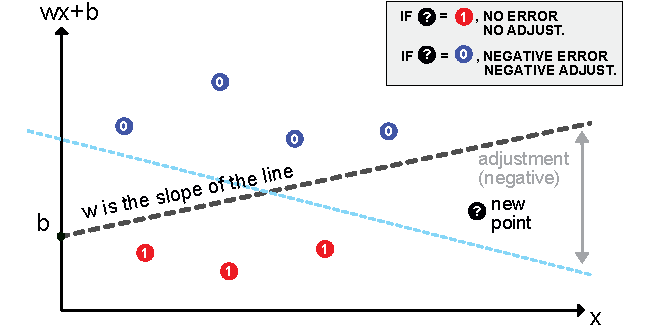
\includegraphics[width=0.7\linewidth]{files/NN_percep_scheme-0f68ea3e26672006d3f08b7ad43f9b31.pdf}

\subsubsection{Multilayer perceptron}

\paragraph{Introduction and notations}

A perceptron can be viewed as a linear model to which is applied a particular function: the Heaviside (step) function. Other choices of functions are naturally possible. In the NN jargon, they are called activation functions. Their purpose is to introduce nonlinearity in otherwise very linear models.

Just like for random forests with trees, the idea behind neural networks is to combine perceptron-like building blocks.

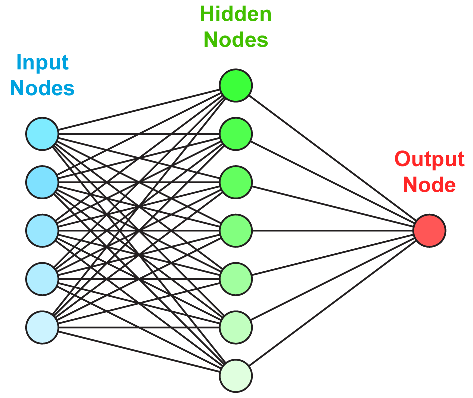
\includegraphics[width=0.7\linewidth]{files/nn-a2dde54f7cb0c2b9c548a1323f3b25c8.pdf}

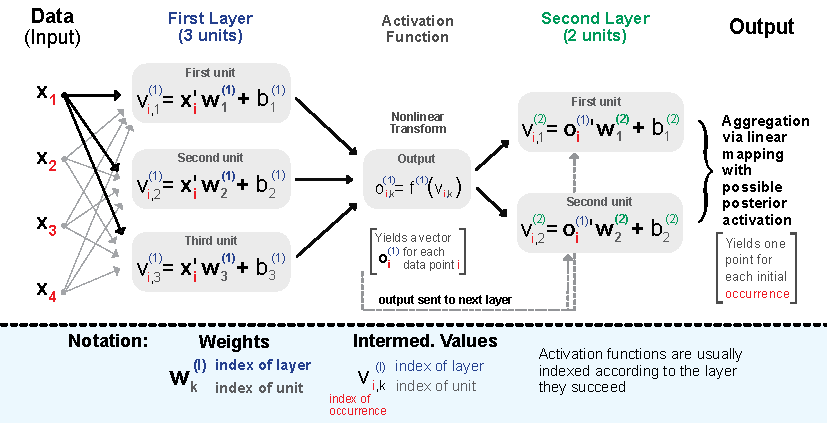
\includegraphics[width=0.7\linewidth]{files/NN_scheme-ac4550766019d6a831579fbda63be208.pdf}

The process is the following. When entering the network, the data goes though the initial linear mapping:\newline
\begin{equation}
v_{i,k}^{(1)}=\textbf{x}_i'\textbf{w}^{(1)}_k+b_k^{(1)},  \text{for } l=1, \quad k \in [1,U_1],
\end{equation}
\newline
which is then transformed by a non-linear function $f^{1}$.

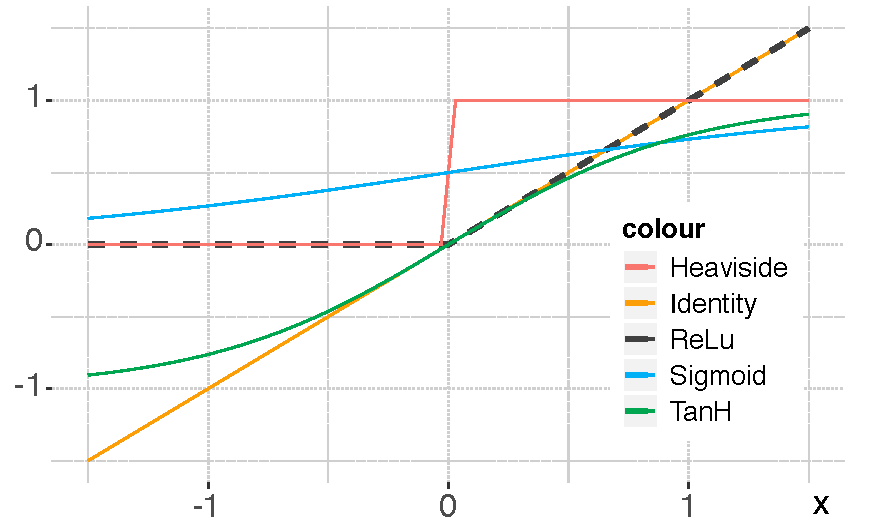
\includegraphics[width=0.7\linewidth]{files/activation-ce4d0d01bdbe93148a34dd7831f38a1e.pdf}

\paragraph{Universal approximation}

One reason neural networks work well is that they are \textit{universal approximators}. Given any bounded continuous function, there exists a one-layer network that can approximate this function up to arbitrary precision.

\begin{equation}
\mathbb{E}\left[(f(x)-f_n(x))^2 \right]=\underbrace{O\left(\frac{c_f}{n} \right)}_{\text{size of network}}+\ \underbrace{O\left(\frac{nK \log(N)}{N} \right)}_{\text{size of sample}},
\end{equation}

\paragraph{Learning via back-propagation}\label{backprop}

Just like for tree methods, neural networks are trained by minimizing some loss function subject to some penalization:
\begin{equation}
O=\sum_{i=1}^I \text{loss}(y_i,\tilde{y}_i)+ \text{penalization},
\end{equation}

The updating of the weights will be performed via gradient descent:

\begin{equation}
\textbf{W} \leftarrow \textbf{W}-\eta  \frac{\partial D(\tilde{y}_i) }{\partial \textbf{W}}.
\end{equation}

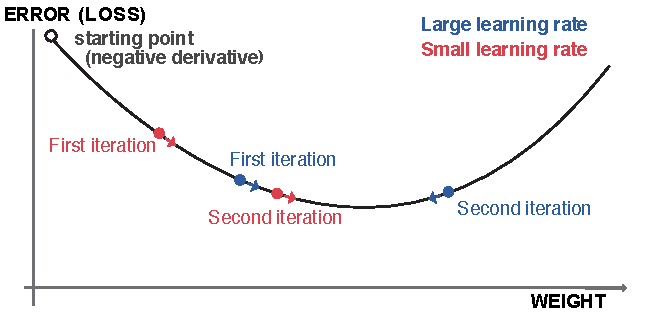
\includegraphics[width=0.7\linewidth]{files/Newton-f185a77ed7d0bde9f6bd8f5d61721a2f.pdf}

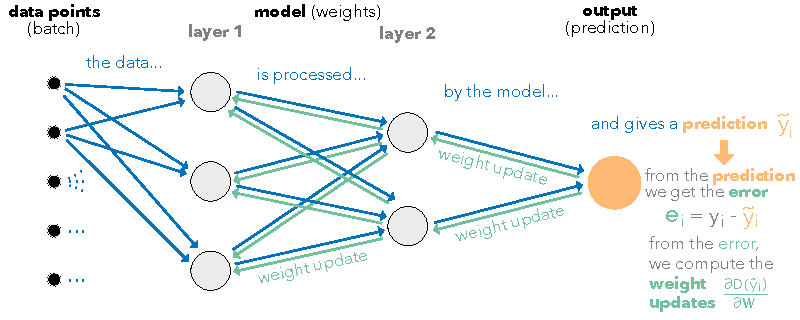
\includegraphics[width=0.7\linewidth]{files/backprop-910104d5ca67cadfed531a35130ca7bc.pdf}

\paragraph{Further details on classification}\label{NNclass}

Facing a classification problem, the trick is to use an appropriate activation function at the very end of the network. The most commonly used activation is the so-called \textit{softmax} function:

\begin{equation}
\tilde{\textbf{y}}_i=s(\textbf{x})_i=\frac{e^{x_i}}{\sum_{j=1}^Je^{x_j}}.
\end{equation}

The cross-entropy is defined as:

\begin{equation}
\text{CE}(\textbf{y}_i,\tilde{\textbf{y}}_i)=-\sum_{j=1}^J\log(\tilde{y}_{i,j})y_{i,j}.
\end{equation}

\subsubsection{How deep we should go and other practical issues}\label{howdeep}

\paragraph{Architectural choices}

The number of hidden layers in current financial applications rarely exceeds three or four. The number of units per layer $(U_k)$ is often chosen to follow the geometric pyramid rule:
\begin{equation}
U_k\approx \left\lfloor O\left( \frac{I}{O}\right)^{\frac{L+1-k}{L+1}}\right\rfloor.
\end{equation}

\paragraph{Penalizations and dropout}

\begin{equation}
O=\sum_{i=1}^I \text{loss}(y_i,\tilde{y}_i)+ \sum_{k} \lambda_k||\textbf{W}_k||_1+ \sum_j\delta_j||\textbf{W}_j||_2^2,
\end{equation}

\subsubsection{Code samples and comments for vanilla MLP}

\paragraph{Regression example}

Before we head to the core of the NN, a short stage of data preparation is required.

\begin{verbatim}
import numpy as np
import pandas as pd
import matplotlib.pyplot as plt
import warnings
warnings.filterwarnings('ignore')
plt.style.use('seaborn-v0_8-whitegrid')
\end{verbatim}

\begin{verbatim}
import os
os.environ["KERAS_BACKEND"] = "jax"  # or "torch"

import keras
from keras import layers
\end{verbatim}

\begin{verbatim}
from keras import layers, regularizers, constraints, initializers, callbacks

from data_build import generate_data
data_ml, features, features_short, returns, stock_ids, stock_ids_short = generate_data()
features_short =["Div_yld", "EPS", "size_avg_252d", "mom_252", "OCF_Growth_1Y", "PB", "vol_252"]
separation_date = "2017-01-15"

# Data preparation
data_ml_clean = data_ml.dropna()
training_sample = data_ml_clean[data_ml['date'] <= separation_date]
testing_sample = data_ml_clean[data_ml['date'] > separation_date] 
NN_train_features = training_sample[features].values    # Training features
NN_train_labels = training_sample['R1M'].values         # Training labels
NN_test_features = testing_sample[features].values      # Testing features
NN_test_labels = testing_sample['R1M'].values           # Testing labels
\end{verbatim}

In Keras, the training of neural networks is performed through three steps: defining the structure, setting the loss function, and training.

\begin{verbatim}
# Define the structure of the network
model = keras.Sequential([
    layers.Dense(units=16, activation='relu', input_shape=(NN_train_features.shape[1],)),
    layers.Dense(units=8, activation='tanh'),
    layers.Dense(units=1)  # No activation means linear activation: f(x) = x
])
\end{verbatim}

\begin{verbatim}
# Model specification
model.compile(
    loss='mean_squared_error',
    optimizer='rmsprop',
    metrics=['mean_absolute_error']
)
model.summary()
\end{verbatim}

\begin{verbatim}
Model: "sequential"
\end{verbatim}

\begin{verbatim}
+---------------------------------+------------------------+---------------+
| Layer (type)                    | Output Shape           |       Param # |
+---------------------------------+------------------------+---------------+
| dense (Dense)                   | (None, 16)             |         1,968 |
+---------------------------------+------------------------+---------------+
| dense_1 (Dense)                 | (None, 8)              |           136 |
+---------------------------------+------------------------+---------------+
| dense_2 (Dense)                 | (None, 1)              |             9 |
+---------------------------------+------------------------+---------------+
\end{verbatim}

\begin{verbatim}
Total params: 2,113 (8.25 KB)
\end{verbatim}

\begin{verbatim}
Trainable params: 2,113 (8.25 KB)
\end{verbatim}

\begin{verbatim}
Non -trainable params: 0 (0.00 B)
\end{verbatim}

\begin{verbatim}
# Train the model
history = model.fit(
    NN_train_features, NN_train_labels,
    epochs=10, batch_size=512,
    validation_data=(NN_test_features, NN_test_labels)
)

# Plot training history
fig, axes = plt.subplots(1, 2, figsize=(12, 4))
axes[0].plot(history.history['loss'], label='Training')
axes[0].plot(history.history['val_loss'], label='Validation')
axes[0].set_xlabel('Epoch'); axes[0].set_ylabel('Loss'); axes[0].legend()
axes[1].plot(history.history['mean_absolute_error'], label='Training')
axes[1].plot(history.history['val_mean_absolute_error'], label='Validation')
axes[1].set_xlabel('Epoch'); axes[1].set_ylabel('MAE'); axes[1].legend()
plt.tight_layout(); plt.show()
\end{verbatim}

\begin{verbatim}
447/447 -------------------- 1s 1ms/step - loss: 5.6226e-04 - mean_absolute_error: 0.0211 - val_loss: 4.0773e-04 - val_mean_absolute_error: 0.0170
\end{verbatim}

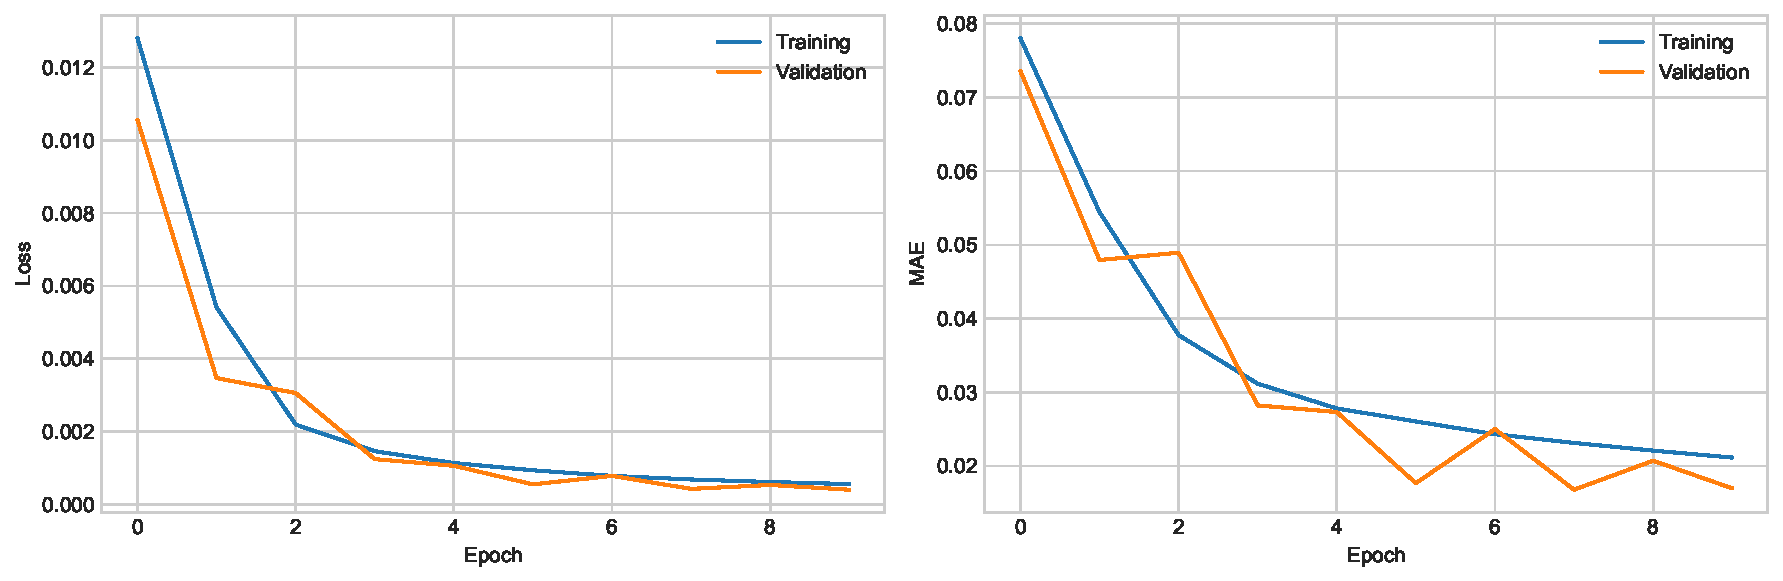
\includegraphics[width=0.7\linewidth]{files/5929b3f3ca8e2c9e99c5ade01646d8a0.pdf}

\begin{verbatim}
# Predictions and hit ratio
predictions = model.predict(NN_test_features).flatten()
hit_ratio = np.mean(predictions * NN_test_labels > 0)
print(f"Hit ratio: {np.round(hit_ratio, 5)}")
\end{verbatim}

\begin{verbatim}
4266/4266 -------------------- 1s 167us/step
\end{verbatim}

\begin{verbatim}
Hit ratio: 0.92084
\end{verbatim}

\paragraph{Classification example}

We pursue our exploration of neural networks with a classification task on the binary label R1M\_C.

\begin{verbatim}
# One-hot encoding of the labels
NN_train_labels_C = pd.get_dummies(training_sample['R1M_C']).values
NN_test_labels_C = pd.get_dummies(testing_sample['R1M_C']).values
\end{verbatim}

\begin{verbatim}
# Define the structure with additional features
model_C = keras.Sequential([
    layers.Dense(units=16, activation='tanh',
                 input_shape=(NN_train_features.shape[1],),
                 kernel_initializer='random_normal',
                 kernel_constraint=constraints.NonNeg()),
    layers.Dropout(rate=0.25),
    layers.Dense(units=8, activation='elu',
                 bias_initializer=initializers.Constant(0.2),
                 kernel_regularizer=regularizers.l2(0.01)),
    layers.Dense(units=2, activation='softmax')
])
\end{verbatim}

\begin{verbatim}
# Model specification
model_C.compile(
    loss='binary_crossentropy',
    optimizer=keras.optimizers.Adam(learning_rate=0.005, beta_1=0.9, beta_2=0.95),
    metrics=['categorical_accuracy']
)
model_C.summary()
\end{verbatim}

\begin{verbatim}
Model: "sequential_1"
\end{verbatim}

\begin{verbatim}
+---------------------------------+------------------------+---------------+
| Layer (type)                    | Output Shape           |       Param # |
+---------------------------------+------------------------+---------------+
| dense_3 (Dense)                 | (None, 16)             |         1,968 |
+---------------------------------+------------------------+---------------+
| dropout (Dropout)               | (None, 16)             |             0 |
+---------------------------------+------------------------+---------------+
| dense_4 (Dense)                 | (None, 8)              |           136 |
+---------------------------------+------------------------+---------------+
| dense_5 (Dense)                 | (None, 2)              |            18 |
+---------------------------------+------------------------+---------------+
\end{verbatim}

\begin{verbatim}
Total params: 2,122 (8.29 KB)
\end{verbatim}

\begin{verbatim}
Trainable params: 2,122 (8.29 KB)
\end{verbatim}

\begin{verbatim}
Non -trainable params: 0 (0.00 B)
\end{verbatim}

\begin{verbatim}
# Train with early stopping
early_stop = callbacks.EarlyStopping(monitor='val_loss', min_delta=0.001, patience=3, verbose=0)

history_C = model_C.fit(
    NN_train_features, NN_train_labels_C,
    epochs=20, batch_size=512,
    validation_data=(NN_test_features, NN_test_labels_C),
    verbose=0, callbacks=[early_stop]
)

# Plot
fig, axes = plt.subplots(1, 2, figsize=(12, 4))
axes[0].plot(history_C.history['loss'], label='Training')
axes[0].plot(history_C.history['val_loss'], label='Validation')
axes[0].set_xlabel('Epoch'); axes[0].set_ylabel('Loss'); axes[0].legend()
axes[1].plot(history_C.history['categorical_accuracy'], label='Training')
axes[1].plot(history_C.history['val_categorical_accuracy'], label='Validation')
axes[1].set_xlabel('Epoch'); axes[1].set_ylabel('Accuracy'); axes[1].legend()
plt.tight_layout(); plt.show()
\end{verbatim}

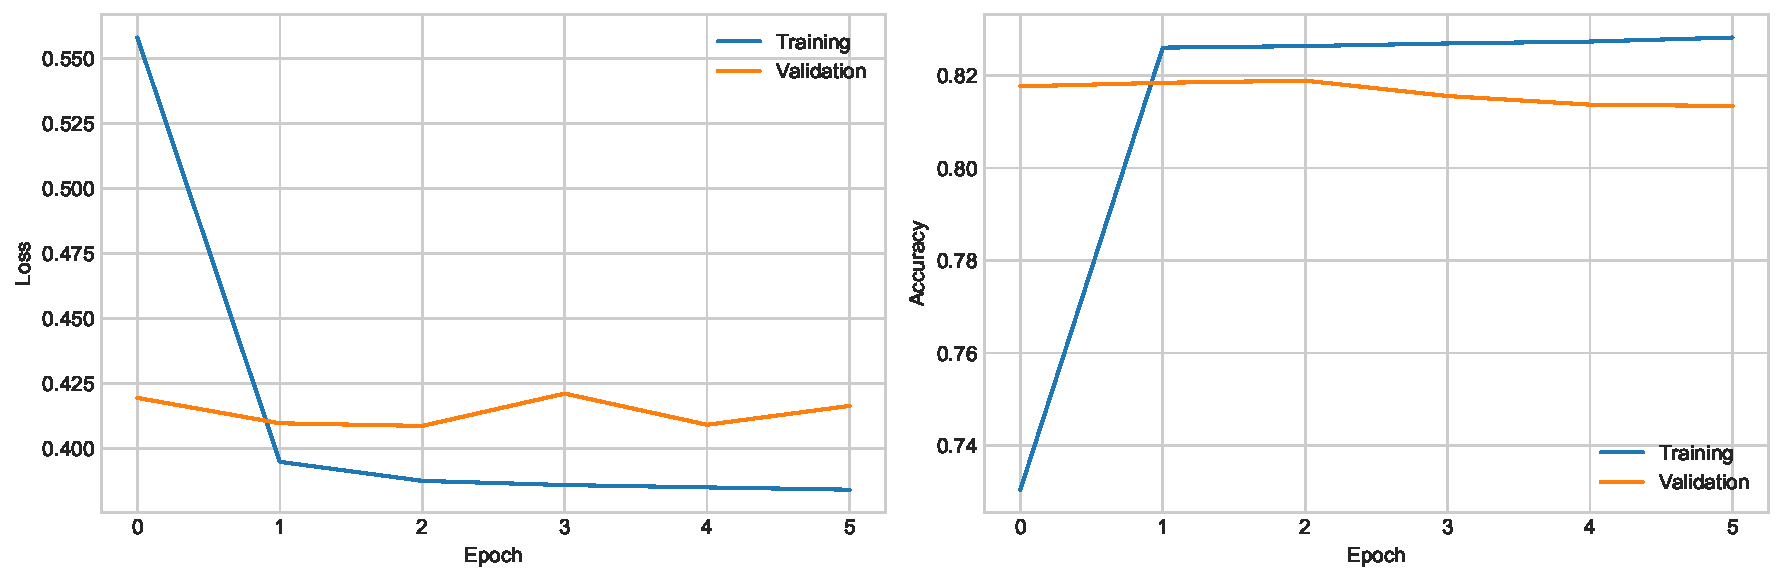
\includegraphics[width=0.7\linewidth]{files/d5aca84fc56e33c0829d122e108a4aa2.pdf}

\paragraph{Custom losses}\label{custloss}

In Keras, it is possible to define user-specified loss functions.

\begin{verbatim}
import keras.ops as ops

def custom_loss(y_true, y_pred):
    var_pred = ops.mean((y_pred - ops.mean(y_pred)) * (y_pred - ops.mean(y_pred)))
    cov_term = ops.mean((y_true - ops.mean(y_true)) * (y_pred - ops.mean(y_pred)))
    return var_pred - 5 * cov_term

model_custom = keras.Sequential([
    layers.Dense(units=16, activation='relu', input_shape=(NN_train_features.shape[1],)),
    layers.Dense(units=8, activation='sigmoid'),
    layers.Dense(units=1)
])

model_custom.compile(loss=custom_loss, optimizer='rmsprop', metrics=['mean_absolute_error'])
\end{verbatim}

\begin{verbatim}
# Train and evaluate
history_custom = model_custom.fit(
    NN_train_features, NN_train_labels,
    epochs=10, batch_size=512,
    validation_data=(NN_test_features, NN_test_labels)
)

predictions_custom = model_custom.predict(NN_test_features).flatten()
hit_ratio_custom = np.mean(predictions_custom * NN_test_labels > 0)
print(f"Hit ratio: {hit_ratio_custom}")
\end{verbatim}

\begin{verbatim}
4266/4266 -------------------- 1s 159us/step
\end{verbatim}

\begin{verbatim}
Hit ratio: 0.5995076995208861
\end{verbatim}

\subsubsection{Recurrent networks}\label{RNN}

\paragraph{Presentation}

Multilayer perceptrons are feed-forward networks because the data flows from left to right with no looping in between. For some particular tasks with sequential linkages, it might be useful to keep track of what happened with the previous sample.

\begin{equation}
\begin{aligned}
\tilde{y}_i&=f^{(y)}\left(\sum_{j=1}^{U_1}h_{i,j}w^{(y)}_j+b^{(2)}\right) \\
\textbf{h}_{i} &=f^{(h)}\left(\sum_{k=1}^{U_0}x_{i,k}w^{(h,1)}_k+b^{(1)}+ \underbrace{\sum_{k=1}^{U_1}  w^{(h,2)}_{k}h_{i-1,k}}_{\text{memory part}} \right),
\end{aligned}
\end{equation}

For a recent theoretical treatment, \cite{chen2026recurrent} derive statistical guarantees for recurrent networks under a broad class of nonlinear autoregressive processes with exogenous variables. They show that recurrence lets the network summarize the past through a compact hidden state instead of many explicit lags, which speeds up estimation compared to standard nonparametric regression.

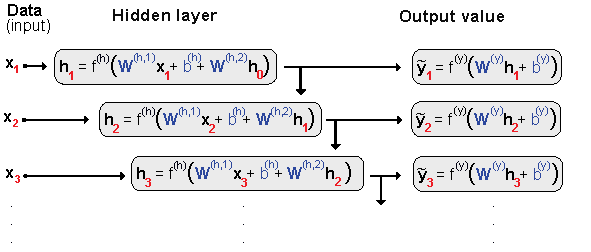
\includegraphics[width=0.7\linewidth]{files/RN-949eb92349432c0d079d12ac88f01871.pdf}

The Gated Recurrent Unit (GRU) has the following representation:
\begin{equation}
\begin{aligned}
\tilde{y}_i&=z_i\tilde{y}_{i-1}+ (1-z_i)\tanh \left(\textbf{w}_y'\textbf{x}_i+ b_y+ u_yr_i\tilde{y}_{i-1}\right) \\
z_i &= \text{sig}(\textbf{w}_z'\textbf{x}_i+b_z+u_z\tilde{y}_{i-1}) \\
r_i &= \text{sig}(\textbf{w}_r'\textbf{x}_i+b_r+u_r\tilde{y}_{i-1})
\end{aligned}
\end{equation}

\paragraph{Code and results}

\begin{verbatim}
# Dedicated dataset for RNN
data_rnn = data_ml[data_ml['fsym_id'].isin(stock_ids_short)]
training_sample_rnn = data_rnn[data_rnn['date'] < separation_date]
testing_sample_rnn = data_rnn[data_rnn['date'] > separation_date]

nb_stocks = len(stock_ids_short)
nb_feats = len(features)
nb_dates_train = len(training_sample_rnn) // nb_stocks
nb_dates_test = len(testing_sample_rnn) // nb_stocks
\end{verbatim}

\begin{verbatim}
# Format the data into arrays: (stock, date, feature)
train_features_rnn = training_sample_rnn[features].values.reshape(nb_stocks, nb_dates_train, nb_feats)
test_features_rnn = testing_sample_rnn[features].values.reshape(nb_stocks, nb_dates_test, nb_feats)
train_labels_rnn = training_sample_rnn['R1M'].values.reshape(nb_stocks, nb_dates_train, 1)
test_labels_rnn = testing_sample_rnn['R1M'].values.reshape(nb_stocks, nb_dates_test, 1)
\end{verbatim}

\begin{verbatim}
# Define the RNN model
model_RNN = keras.Sequential([
    layers.GRU(units=16, 
               #input_batch_size=nb_stocks,
               #input_shape=(nb_dates_train, nb_feats),
               activation='tanh', return_sequences=True),
    layers.Dense(units=1)
])

model_RNN.compile(loss='mean_squared_error', optimizer='rmsprop', metrics=['mean_absolute_error'])
\end{verbatim}

\begin{verbatim}
# Train the RNN model
history_RNN = model_RNN.fit(
    train_features_rnn, train_labels_rnn,
    epochs=10, batch_size=nb_stocks, verbose=0
)
\end{verbatim}

\begin{verbatim}
pred_rnn = model_RNN.predict(test_features_rnn, batch_size=nb_stocks)
hit_ratio_rnn = np.mean(pred_rnn.flatten() * test_labels_rnn.flatten() > 0)
print(f"Hit ratio: {hit_ratio_rnn}")
\end{verbatim}

\begin{verbatim}
1/1 -------------------- 0s 140ms/step
\end{verbatim}

\begin{verbatim}
Hit ratio: 0.4964004687761594
\end{verbatim}

\subsubsection{Other common architectures}

\paragraph{Generative adversarial networks}\label{generative-aversarial-networks}

GANs consist in two neural networks: the first one tries to learn and the second one tries to fool the first. $D$ and $G$ play the following minimax game:
\begin{equation}
\underset{G}{\min} \ \underset{D}{\max} \ \left\{ \mathbb{E}[\log(D(\textbf{x}))]+\mathbb{E}[\log(1-D(G(\textbf{z})))] \right\}.
\end{equation}

\paragraph{Autoencoders}\label{autoencoders}

AEs are a family of neural networks where the label is equal to the input:
\begin{equation}
\begin{array}{ccccccccc}
\textbf{x} & &\overset{E}{\longrightarrow} && \textbf{z} && \overset{D}{\longrightarrow} && \textbf{x}' \\
\text{input} && \text{encoder} && \text{code} && \text{decoder} && \text{modified input}
\end{array}
\end{equation}

\cite{xiu2025autoencoders} establish theoretical guarantees for deep autoencoders in a nonlinear factor model. They show that the extracted codes converge to the true latent factors as the panel grows, and extend the result to supervised autoencoders used for factor augmented prediction, with applications to macroeconomic forecasting and asset return prediction.

\paragraph{A word on convolutional networks}\label{CNN}

CNNs allow to progressively reduce the dimension of a large dataset by keeping local information. The output values are given by:
\begin{equation}
o_{i,k}=\sum_{j=1}^J\sum_{l=1}^Lw_{j,l}x_{i+j-1,k+l-1}.
\end{equation}

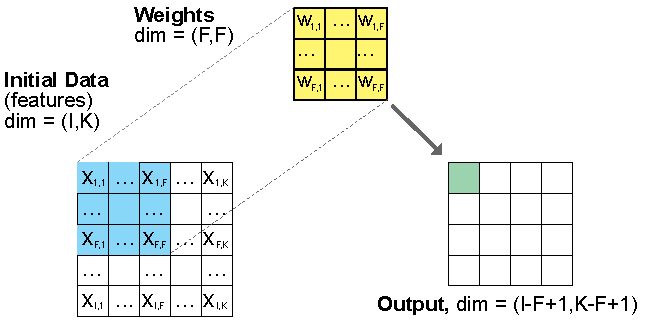
\includegraphics[width=0.7\linewidth]{files/cnn_scheme-8eb3e854b25a4e59e943b02e8593c6c9.pdf}

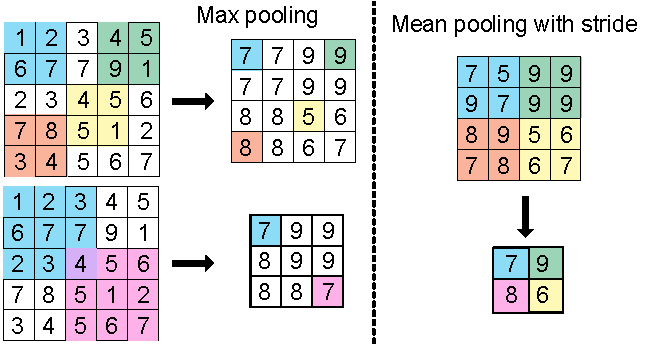
\includegraphics[width=0.7\linewidth]{files/cnn_pooling-05c87ceec9f840058ff626ad473215fa.pdf}

\subsubsection{Foundation models for tabular data}\label{foundation-tabular}

\paragraph{Presentation}

Foundation models pretrain a single large network once, often on synthetic data, and then adapt to a brand new task with no further gradient updates. This paradigm is well known for text and images and has recently reached tabular data. A pretrained transformer reads the whole training table as context and the test rows as a query, then returns predictions in one forward pass. There is no loss to minimize and no hyperparameter to tune at deployment time.

\cite{grinsztajn2022why} show that tree based models still beat plain deep networks on typical tabular data. This finding motivates a dedicated pretrained architecture rather than a generic network trained from scratch. \cite{hollmann2025accurate} introduce TabPFN, a transformer pretrained on millions of synthetic datasets that matches or beats tuned gradient boosting on small tables. \cite{qu2025tabicl} extend the idea with TabICL, a model built by the Inria team behind scikit learn, which scales in context learning to much larger tables through a two stage column then row attention mechanism.

For factor investing, this paradigm is appealing. Each rebalancing date can be treated as a small fresh dataset. The model reads the past cross section as context and predicts the next one, with no retraining between dates. Below, we illustrate this idea with TabICL. We pick this library because it installs with one pip command, downloads open weights with no license step, and handles regression directly.

The exercise below is a genuine out of sample test. For each test month $t$, the model is fit only on the single prior month and then applied to month $t$ features. Recall that in this book, \texttt{R1M} is dated at $t$ but stores the forward return realised between $t$ and $t+1$. So the model never sees the outcome it is scored on. We report two metrics. The first is the \textbf{information coefficient}, the cross sectional correlation between predicted and realised \texttt{R1M}. The second is the \textbf{long short decile Sharpe ratio}: each month we go long the top decile of predictions and short the bottom decile, and we annualise the mean and standard deviation of these twelve monthly spread returns.

\paragraph{Code and results}

\begin{verbatim}
import time
from sklearn.preprocessing import StandardScaler
from sklearn.linear_model import Ridge
from tabicl import TabICLRegressor

dates_sorted = sorted(data_ml_clean['date'].unique())
test_dates = dates_sorted[-13:-1]   # 12 rolling rebalancing dates

records = []
t0 = time.time()
for td in test_dates:
    idx = dates_sorted.index(td)
    train_date = dates_sorted[idx - 1]              # the single month strictly before td
    assert train_date < td                           # no look ahead: train date precedes test date

    Xtr = data_ml_clean.loc[data_ml_clean['date'] == train_date, features_short].values
    ytr = data_ml_clean.loc[data_ml_clean['date'] == train_date, 'R1M'].values
    Xte = data_ml_clean.loc[data_ml_clean['date'] == td, features_short].values
    yte = data_ml_clean.loc[data_ml_clean['date'] == td, 'R1M'].values   # forward return, unknown at td

    sc = StandardScaler().fit(Xtr)
    Xtr_s, Xte_s = sc.transform(Xtr), sc.transform(Xte)

    tab_mod = TabICLRegressor().fit(Xtr_s, ytr)
    pred_tab = tab_mod.predict(Xte_s)                # built only from Xte, the info available at td

    ridge_mod = Ridge(alpha=1.0).fit(Xtr_s, ytr)
    pred_ridge = ridge_mod.predict(Xte_s)

    q10t, q90t = np.percentile(pred_tab, [10, 90])
    q10r, q90r = np.percentile(pred_ridge, [10, 90])

    records.append({
        'date': td, 'train_date': train_date,
        'ic_tab': np.corrcoef(pred_tab, yte)[0, 1],
        'ic_ridge': np.corrcoef(pred_ridge, yte)[0, 1],
        'ls_tab': yte[pred_tab >= q90t].mean() - yte[pred_tab <= q10t].mean(),
        'ls_ridge': yte[pred_ridge >= q90r].mean() - yte[pred_ridge <= q10r].mean(),
    })

elapsed = time.time() - t0
res = pd.DataFrame(records)

# mean, std and Sharpe are reported separately so the computation is checkable
mu_tab, sd_tab = res['ls_tab'].mean(), res['ls_tab'].std()
mu_ridge, sd_ridge = res['ls_ridge'].mean(), res['ls_ridge'].std()
sharpe_tab = mu_tab / sd_tab * np.sqrt(12)
sharpe_ridge = mu_ridge / sd_ridge * np.sqrt(12)

print(f"Rebalancing dates covered   : {len(test_dates)}")
print(f"Total wall time             : {elapsed:.1f} seconds")
print(f"Train date always before test date : {(res['train_date'] < res['date']).all()}")
print()
print("Information coefficient (corr. between prediction and realised forward R1M):")
print(f"  TabICL : {res['ic_tab'].mean():.4f}")
print(f"  Ridge  : {res['ic_ridge'].mean():.4f}")
print()
print("Long short decile portfolio, monthly spread return statistics (12 test months):")
print(f"  TabICL : mean={mu_tab:.4f}  std={sd_tab:.4f}  annualised Sharpe={sharpe_tab:.2f}")
print(f"  Ridge  : mean={mu_ridge:.4f}  std={sd_ridge:.4f}  annualised Sharpe={sharpe_ridge:.2f}")
\end{verbatim}

\begin{verbatim}
Rebalancing dates covered   : 12
Total wall time             : 53.1 seconds
Train date always before test date : True

Information coefficient (corr. between prediction and realised forward R1M):
  TabICL : -0.0090
  Ridge  : -0.0144

Long short decile portfolio, monthly spread return statistics (12 test months):
  TabICL : mean=-0.0092  std=0.0730  annualised Sharpe=-0.44
  Ridge  : mean=-0.0076  std=0.0693  annualised Sharpe=-0.38
\end{verbatim}

The check above confirms every fold trains strictly before it tests, so the numbers are out of sample by construction, not synchronous. Both Sharpe ratios are negative. This is worth underlining: a negative Sharpe means the long short strategy loses money on average over these twelve months, for both models. This illustrates one of the recurring messages of this book: machine learning in finance is not a plug and play exercise. A powerful state-of-the-art model does not automatically produce good returns. Turning a model into profits takes careful feature engineering, thoughtful validation, sensible portfolio construction, and plain domain expertise. None of that is present in the minimal setup used here. Note also that TabICL involves some internal randomness, so rerunning this cell can shift the numbers slightly without changing the overall picture.

\subsubsection{Coding exercises}

\begin{enumerate}
\item Code the autoencoder model described in \cite{gu2019autoencoder} using the functional API.
\item Demonstrate the universal approximation of simple NNs by approximating sin(x) over [0,6] with 16 and then 128 units.
\end{enumerate}

\subsection{Graph neural networks}

% 
% Version: 0.7.4
% Last updated: 2026-08-05
% Restructured shipping draft of Chapter 9, following the flow of the 1st-edition
% Neural networks chapter (mlfactor.com/NN.html): general principle -> GNN-specific
% issues -> one worked illustration -> other families -> exercises. The full long
% draft (Chapter_9_Graph_Neural_Networks.md, v0.26.1) is retained as the source of
% truth for future work. The notebook runs end to end unaided: the loader, the models,
% the depth sweep, the five-seed walk-forward and LightGBM are all executed, and every
% figure (9.1 depth, 9.2 cumulative IC, 9.3 seed dispersion) is produced by the
% notebook's own plotting code, so there are no orphan PNGs. Verified via verify_outputs
% -> OUTPUTS=MATCH, STATUS=OK (10 cells, 0 failed). TABLE 9.1 (the GCN ablation row) and
% its paired-t and Newey-West statistics are now produced by the notebook from the
% seed-by-seed ICs; the GATv2/GraphSAGE comparison is stated qualitatively, and the
% compact "what survives" checks summarise the long draft's fuller experiments. Every
% number and figure traces to executed, seeded code.
% 
% Target ToC:
%   9.1 Introduction
%   9.2 The graph convolutional network            (general principle)
%   9.3 Dealing with GNN-specific issues           (building the graph; over-smoothing;
%                                                    over-squashing/heterophily; tabular handicap)
%   9.4 A GNN on the equity panel                  (illustration: from scratch + PyG; benchmark;
%                                                    the ablation and what survives)
%   9.5 Other families of graph models            (GraphSAGE/GAT/GATv2; GIN/R-GCN; temporal)
%   9.6 Interpretability (short)
%   9.7 Coding exercises
%

\subsubsection{Introduction}\label{sec_gnn_intro}

Graph neural networks (GNNs) are a rich and fast-moving topic. In this chapter we introduce the simple ideas behind the most common architectures and put them to work on the equity panel that runs through the book. For a broad survey of the machinery we refer the interested reader to \cite{gilmer2017neural}, who unify most variants under a single message-passing formalism; the architectures we build upon are the graph convolutional network of \cite{kipf2017semisupervised}, the inductive framework of \cite{hamilton2017inductive}, and the attention mechanism of \cite{velickovic2018graph}. The implementation rests on the Python graph-learning stack, chiefly PyTorch Geometric (\cite{fey2019fast}), which has no genuine equivalent outside Python; the panel, the features and the notation are unchanged from earlier chapters.

The motivation for a graph is economic. The supervised learners of the previous chapters, from penalized regressions to boosted trees and neural networks, treat each stock at each date as an independent observation. Firms, however, are not independent: they are tied through supply chains, shared industries, common ownership and overlapping analyst coverage, and a long line of research shows these links carry predictive content. The anchor is \cite{cohen2008economic}, who document that news travels slowly along customer and supplier links, so a firm's returns predict its economically connected counterparts with a lag; related effects appear at the industry level (\cite{menzly2010market}) and through shared analyst coverage (\cite{ali2020shared}). If information diffuses across a network of firms, a model that can see that network may forecast better than one that treats each stock in isolation. A GNN is the natural object for exploiting such structure: it represents each date as a graph whose nodes are stocks and whose edges encode economic links, and lets the prediction for a firm borrow from its neighbours before a forecast is issued. The broader case for representing finance as a network of interacting entities, and the machinery for building and analysing such networks, is made in the recent monograph of \cite{konstantinov2025network}.

The application of GNNs to equity prediction is by now a sizeable literature, surveyed by \cite{patel2024systematic}. \cite{feng2019temporal} cast stock selection as ranking over a graph of industry and knowledge-base relations; \cite{kim2019hats} attend hierarchically over relation types from a corporate knowledge base; \cite{xu2021hist} mine information across learned stock concepts; and \cite{capponi2025graph} aggregate characteristics across a supply-chain network. These studies typically report encouraging figures, though it is worth attending to what each is measured against, since a gain over a narrower graph is not a gain over no graph at all. They connect to the broader use of machine learning in asset pricing, where the demanding benchmarks were set by \cite{gu2020empirical} and by the no-arbitrage deep-learning model of \cite{chen2024deep}.

\subsubsection{The graph convolutional network}\label{sec_gnn_gcn}

\paragraph{From a table to a sequence of graphs}\label{sec_gnn_graphs}

Every model in the preceding chapters consumes the panel as a table: one row is a pair (t, n) of a date and an asset, and the features $\mathbf{x}_{t,n}$ of that row are mapped to a label $y_{t,n}$ without reference to the other rows sharing the same date. A graph model changes this in one respect: rows that belong to the same date may communicate. Each date becomes one graph snapshot $\mathcal{G}_t = (\mathcal{V}_t, \mathcal{E}_t)$, whose vertex set $\mathcal{V}_t$ is the $N_t$ firms trading that month and whose edge set $\mathcal{E}_t$ collects the linked pairs $(n,m)$. It carries three objects: the node-feature matrix $\mathbf{X}_t$ of dimension $N_t \times K$, whose row $n$ is the characteristic vector of firm $n$ with $K = 122$; the label vector $\mathbf{y}_t$, whose entry $n$ is the one-month-ahead return; and the adjacency matrix $\mathbf{A}_t$ of dimension $N_t \times N_t$, the matrix form of the edge set, whose entry $(n,m)$ is nonzero exactly when $(n,m) \in \mathcal{E}_t$, that is, when firms $n$ and $m$ are linked. The node set changes month to month as firms enter and exit, so the model must be inductive, and the panel contains no edges of its own: $\mathbf{A}_t$ must be supplied from outside, a modelling choice we take up in Section~\ref{sec_gnn_issues}.

\paragraph{Message passing and the propagation rule}\label{sec_gnn_message}

The operation at the centre of these models is message passing, and it is close to the neural networks of the previous chapter. Where a multilayer perceptron transforms a firm's own characteristics through activated linear maps, a GNN interleaves those maps with an aggregation step that mixes each node's representation with a summary of its neighbours. \cite{gilmer2017neural} observe that most graph architectures share one form: writing $\mathbf{o}_{t,n}^{(l)}$ for the representation of node $n$ at layer $l$ and $\mathcal{N}(n)$ for its neighbours, a layer updates each node from itself and an aggregate of its neighbourhood,

\begin{equation}
\label{eq_gnn_1}
\mathbf{o}_{t,n}^{(l+1)} = \text{update}\Big( \mathbf{o}_{t,n}^{(l)},\ \bigoplus_{m \in \mathcal{N}(n)} \text{message}\big(\mathbf{o}_{t,n}^{(l)}, \mathbf{o}_{t,m}^{(l)}\big) \Big).
\end{equation}

The variants differ in the aggregator $\bigoplus$. The canonical instance is the graph convolutional network of \cite{kipf2017semisupervised}, the practical end of a spectral lineage running from \cite{bruna2014spectral} through the localized polynomial filters of \cite{defferrard2016convolutional}. Writing $\tilde{\mathbf{A}} = \mathbf{A} + \mathbf{I}$ for the adjacency with self-loops and $\tilde{\mathbf{D}}$ for its degree matrix, one layer is

\begin{equation}
\label{eq_gnn_2}
\mathbf{H}^{(l+1)} = f^{(l)}\!\left( \tilde{\mathbf{D}}^{-1/2}\tilde{\mathbf{A}}\tilde{\mathbf{D}}^{-1/2}\,\mathbf{H}^{(l)}\mathbf{W}^{(l)} \right), \qquad \mathbf{H}^{(0)} = \mathbf{X}_t.
\end{equation}

Equation \ref{eq_gnn_2} is a multilayer perceptron in which, at every layer, each firm's representation is replaced by a weighted average of itself and its neighbours. Since the matrix that premultiplies $\mathbf{H}^{(l)}\mathbf{W}^{(l)}$ is a smoothing operator, a GCN is, in the terms of \cite{nt2019revisiting}, a low-pass filter on node features: it attenuates the components of the signal that oscillate across edges and keeps those that vary slowly. This already contains the difficulty the chapter runs into. On a graph that links firms in the same industry, the smoothest signals are the ones constant within each industry, which are precisely the signals that say nothing about which firm within an industry will outperform. A low-pass filter on such a graph preserves industry-level quantities and erases the cross-sectional dispersion a stock-selection signal needs.

\paragraph{The graph-free limit and the ablation}\label{sec_gnn_ablation}

Equation \ref{eq_gnn_2} makes the chapter's organising experiment transparent. Setting $\mathbf{A}_t = \mathbf{I}$ removes the neighbour averaging and returns the propagation rule to the multilayer perceptron of Chapter 8. The adjacency is therefore the only thing separating a graph model from a graph-free one of the same shape, so we ask whether the graph helps by comparing the two directly, holding the architecture and the parameter count fixed. The permutation-invariant Deep Sets model of \cite{zaheer2017deep}, which pools the whole cross-section without any edge, is the same limit reached from the other side. These graph-free models are not a formality; they are the controls against which every result in Section~\ref{sec_gnn_panel} is judged, and they turn out to be decisive.

\subsubsection{Dealing with GNN-specific issues}\label{sec_gnn_issues}

Three things separate a GNN from the models of the previous chapters, and each raises a difficulty of its own: the graph must be built, message passing has failure modes that theory predicts, and the underlying task is tabular, a regime in which deep models rarely lead.

\paragraph{Building the equity graph}\label{sec_gnn_building}

Nothing in the panel says which firms are connected; the adjacency must be constructed, and the literature offers a wide menu with different data requirements and different exposure to look-ahead bias. The most common choice is an industry classification: two firms are linked when they share a NAICS sector. It is static and therefore free of look-ahead, available in our data, and economically motivated by the industry-momentum evidence of \cite{moskowitz1999industries}. Other families build edges from supply chains (\cite{cohen2008economic}), from price co-movement over a trailing window (\cite{xiang2022temporal}), from characteristic similarity, or learn the graph inside the model (\cite{cheng2021modeling}); a systematic account, from correlation and partial-correlation graphs to regression and Granger-causality edges, is given by \cite{konstantinov2025network}. We adopt the sector graph as the running example and take up alternative constructions in the exercises.

Whatever the construction, one measurement governs whether it can help. A graph is homophilous when connected nodes tend to resemble one another, and graph convolution assumes this, since averaging over neighbours is only sensible when neighbours are informative about the node. On the sector graph, connected firms share the sign of their next-month return with probability 0.607, above chance but far from strong, and because the sector graph links every firm in a sector to every other, a firm in the largest sector has several hundred neighbours, so the neighbourhood average is close to the sector mean.

\paragraph{Over-smoothing and depth}\label{sec_gnn_smoothing}

Repeated averaging drives node representations together, the over-smoothing formalised by \cite{li2018deeper}, who show that a graph convolution is a form of Laplacian smoothing and that stacking many layers pushes every node toward a common value. \cite{oono2020graph} make the rate precise: the distance of the representations from that common limit contracts geometrically with depth, at a rate set by the product of the largest singular value of the weight matrix and the second-largest eigenvalue of the normalised adjacency, so on a well-connected graph the collapse is exponential in the number of layers. A representation that does not vary across firms cannot rank them, and on a dense sector graph, where a firm's neighbourhood is close to its whole sector, the effect arrives within a handful of layers. We measure it directly in Section~\ref{sec_gnn_panel}, training the same architecture at increasing depth with and without the edges. The literature does offer remedies, decoupling the propagation from the feature transformation as in APPNP (\cite{gasteiger2019predict}), or adding identity and residual connections as in GCNII (\cite{chen2020simple}), which stays accurate at sixty-four layers where a plain graph convolutional network collapses; but these cure the depth pathology without touching the prior question of whether the graph carries any signal worth propagating. The practical implication for a shallow model, anticipated here, is to keep message passing to one or two layers.

\paragraph{Over-squashing and heterophily}\label{sec_gnn_squashing}

Two further failure modes matter, one about distance and one about the kind of similarity the edges encode. Over-squashing, identified by \cite{alon2021bottleneck}, is the observation that a node's receptive field grows exponentially with the number of hops while the fixed-size vector that must carry it does not, so information from distant nodes is compressed, or squashed, until it is effectively lost; a task that needs many hops to reach the relevant firms cannot be served by message passing. Heterophily is the deeper issue and the one most relevant here. Message passing helps only when neighbours resemble the node in the quantity being predicted, and \cite{platonov2023critical}, on a benchmark built to isolate this, show that the standard architectures lose their advantage, and can fall behind a graph-free baseline, once a graph is heterophilous. The subtlety for equities is that the sector graph is homophilous in the features, since firms in an industry share characteristics, but close to heterophilous in the label, since sharing an industry says little about which firm will out-return the other next month. It sits in an uncomfortable middle: homophilous enough that averaging changes the forecast, not homophilous enough in the return for the change to help.

\paragraph{The tabular-data handicap}\label{sec_gnn_tabular}

Underlying all of this is a blunter fact: predicting the cross-section of returns from characteristics is a tabular problem, and on tabular data deep networks rarely lead. \cite{grinsztajn2022treebased} trace the advantage of gradient boosting to properties of the data that neural networks handle poorly, uninformative features that trees can ignore but a dense network cannot, target functions that are not smooth, and the absence of any rotational structure a network could exploit, all of which describe a panel of firm characteristics. \cite{shwartzziv2022tabular} reach the same verdict across a wide range of datasets. \cite{gu2020empirical} add the finance-specific point that the signal-to-noise ratio in returns is so low that the deepest, most flexible models overfit rather than gain: in their comparison neural network performance peaks at three hidden layers and then declines, so shallower networks beat deeper ones. A GNN does not escape this handicap; it inherits it from the multilayer perceptron at its core and then layers on an inductive bias, message passing over a graph, that was designed for domains such as molecules or citation networks where the edges are given and reliable. Equities offer neither a given graph nor a reliable one, so the prior expectation, before any experiment, should be modest.

\subsubsection{A GNN on the equity panel}\label{sec_gnn_panel}

We now implement the graph convolution on the panel, first from scratch and then in PyTorch Geometric, and benchmark it against a multilayer perceptron and gradient boosting. Every model is refitted annually on an expanding walk-forward window from 2015 to 2026 under five random seeds, and the features are ranked cross-sectionally within each date.

\paragraph{A graph layer from scratch, then in PyTorch Geometric}\label{sec_gnn_scratch}

We first load the panel, rank the features cross-sectionally within each date, and turn each date into a graph snapshot. Reproducibility here needs three ingredients together: the seed, deterministic kernels, and a single compute thread, since the neighbourhood aggregation reduces floating-point values in an order that otherwise varies between runs.

\begin{verbatim}
import os, random, numpy as np, pandas as pd, torch, torch.nn as nn, torch.nn.functional as F
from scipy.stats import spearmanr
os.environ['KMP_DUPLICATE_LIB_OK'] = 'TRUE'; os.makedirs('figures', exist_ok=True)
SEED = 42
def set_seed(seed=SEED):                                   # seed every generator; force determinism
    random.seed(seed); np.random.seed(seed); torch.manual_seed(seed)
    torch.backends.cudnn.deterministic = True; torch.backends.cudnn.benchmark = False
    torch.use_deterministic_algorithms(True, warn_only=True)
    torch.set_num_threads(1)                               # the scatter-add reduces in parallel
set_seed()

data_ml = pd.read_parquet('data/mlfi_us_data.parquet')     # the book's US equity panel
univ = pd.read_csv('data/mlfi_us_universe.csv')            # id -> NAICS sector, the edge source
excl = {'id', 'date', 'R1M_Usd', 'R3M_Usd', 'R6M_Usd', 'R12M_Usd'}
features = [c for c in data_ml.columns if c not in excl and pd.api.types.is_numeric_dtype(data_ml[c])]
panel = data_ml.merge(univ[['id', 'naics_sector_code']], on='id').dropna(
    subset=['R1M_Usd', 'naics_sector_code'])
g = panel.groupby('date')
panel[features] = g[features].rank(pct=True).fillna(0.5) - 0.5      # centred cross-sectional ranks
panel['y_rank'] = (g['R1M_Usd'].rank(pct=True) - 0.5) * 3.464       # unit-variance label
K = len(features)

def snapshots(df):                                         # one graph per date
    out = []
    for dt, blk in df.groupby('date'):
        out.append((dt, torch.tensor(blk[features].values, dtype=torch.float32),
                    torch.tensor(blk['y_rank'].values, dtype=torch.float32),
                    torch.tensor(pd.factorize(blk['naics_sector_code'])[0], dtype=torch.long),
                    blk['R1M_Usd'].values))
    return out
\end{verbatim}

\begin{verbatim}
C:\Users\tguid\AppData\Local\Temp\ipykernel_8832\1876160395.py:20: PerformanceWarning: DataFrame is highly fragmented.  This is usually the result of calling `frame.insert` many times, which has poor performance.  Consider joining all columns at once using pd.concat(axis=1) instead. To get a de-fragmented frame, use `newframe = frame.copy()`
  panel['y_rank'] = (g['R1M_Usd'].rank(pct=True) - 0.5) * 3.464       # unit-variance label
\end{verbatim}

Because the sector graph links every firm in a sector to every other, the neighbour average is exactly the sector mean, computable in $O(N_t)$ by scattering into sector buckets rather than forming a dense adjacency. The graph convolutional layer of equation (9.2) blends a firm with that mean, applies a linear map and a nonlinearity. Written this way the ablation is transparent, since deleting the blend is what setting $\mathbf{A}_t = \mathbf{I}$ does, and we define the edge-free twin by inheritance so it cannot drift.

\begin{verbatim}
def sector_mean(X, sec):                                   # neighbour average over each sector
    S = int(sec.max()) + 1
    sums = torch.zeros(S, X.size(1)).index_add_(0, sec, X)
    cnts = torch.zeros(S).index_add_(0, sec, torch.ones_like(sec, dtype=torch.float32))
    return (sums / cnts.clamp(min=1).unsqueeze(1))[sec]

class DeepGCN(nn.Module):                                  # L message-passing layers
    def __init__(self, k, h=32, L=2):
        super().__init__()
        self.inp = nn.Linear(k, h)
        self.hid = nn.ModuleList([nn.Linear(h, h) for _ in range(max(L - 1, 0))])
        self.out = nn.Linear(h, 1); self.drop = nn.Dropout(0.1)
    def mix(self, H, sec):
        return 0.5 * H + 0.5 * sector_mean(H, sec)         # self-loop plus neighbour average
    def forward(self, X, sec):
        H = self.drop(F.relu(self.inp(self.mix(X, sec))))
        for lin in self.hid:
            H = self.drop(F.relu(lin(self.mix(H, sec))))
        return self.out(H).squeeze(-1)

class DeepGCN_NoGraph(DeepGCN):                            # the A_t = I twin: mix returns H
    def mix(self, H, sec):
        return H
\end{verbatim}

Three quantities the surrounding discussion refers to can be read straight from the data and the model: the number of characteristics, the parameter budget of the two-layer network, and the homophily of the sector graph quoted in Section~\ref{sec_gnn_building}, the last computed as the probability that two firms in a sector share the sign of their next-month return, averaged over dates.

\begin{verbatim}
def homophily(blk):                                        # P(same sign of return | same sector), one date
    num = den = 0.0
    for _, grp in blk.groupby('naics_sector_code'):
        pos = int((grp['R1M_Usd'] > 0).sum()); n = len(grp); neg = n - pos
        num += pos * (pos - 1) / 2 + neg * (neg - 1) / 2; den += n * (n - 1) / 2
    return num / max(den, 1)
print(f'characteristics K            = {K}')
print(f'DeepGCN(K, 32, 2) parameters = {sum(p.numel() for p in DeepGCN(K, 32, 2).parameters())}')
print(f'sector edge homophily        = {np.mean([homophily(b) for _, b in panel.groupby("date")]):.4f}')
\end{verbatim}

\begin{verbatim}
characteristics K            = 122
DeepGCN(K, 32, 2) parameters = 5025
\end{verbatim}

\begin{verbatim}
sector edge homophily        = 0.6072
\end{verbatim}

The panel carries the 122 characteristics used throughout, the two-layer graph network and its edge-free twin share a budget of 5,025 parameters, and the sector graph's homophily is 0.607, the value Section~\ref{sec_gnn_building} relies on.

In practice one would not hand-code these layers. The same model is expressed in PyTorch Geometric by replacing the propagation with the library's operators, which also gives GraphSAGE, GATv2 and the rest at the cost of a single word.

\begin{verbatim}
from torch_geometric.nn import GCNConv, SAGEConv, GATv2Conv
class PyGNet(nn.Module):                                   # swap GCNConv for SAGEConv or GATv2Conv
    def __init__(self, k, h=32, conv=GCNConv):
        super().__init__()
        self.c1, self.c2 = conv(k, h), conv(h, 1)
    def forward(self, x, edge_index):
        return self.c2(F.relu(self.c1(x, edge_index)), edge_index).squeeze(-1)
\end{verbatim}

\begin{verbatim}
C:\Users\tguid\miniconda3\envs\futures_dl\Lib\site-packages\tqdm\auto.py:21: TqdmWarning: IProgress not found. Please update jupyter and ipywidgets. See https://ipywidgets.readthedocs.io/en/stable/user_install.html
  from .autonotebook import tqdm as notebook_tqdm
\end{verbatim}

Training is a squared-error loss on the ranked label over eight passes, seeded before the model is built so results do not depend on call order, and the rank information coefficient is the monthly cross-sectional correlation between forecast and realised return.

\begin{verbatim}
def fit_gnn(build, tr, seed=SEED, epochs=8):               # seed BEFORE building the model
    set_seed(seed); model = build()
    opt = torch.optim.Adam(model.parameters(), lr=0.003)
    rng = np.random.default_rng(seed); order = list(range(len(tr)))
    for _ in range(epochs):
        model.train(); rng.shuffle(order)
        for i in order:
            _, X, y, sec, _ = tr[i]
            opt.zero_grad(); F.mse_loss(model(X, sec), y).backward(); opt.step()
    model.eval(); return model

def ic_series(model, te):                                  # monthly out-of-sample rank IC, by date
    rows = [(dt, spearmanr(model(X, sec).detach().numpy(), raw).statistic)
            for dt, X, _, sec, raw in te]
    return pd.Series({dt: ic for dt, ic in rows if not np.isnan(ic)})
\end{verbatim}

The clearest thing to run first is the over-smoothing prediction of Section~\ref{sec_gnn_smoothing}. We train the same architecture at increasing depth, once with the sector edges and once with them removed, on a fixed split that trains before 2015 and scores from 2015 on.

\begin{verbatim}
tr_fix = snapshots(panel[panel.date < '2015-01-01'])       # train once, then score the rest
te_fix = snapshots(panel[panel.date >= '2015-01-01'])
Ls, ic_graph, ic_nograph = [1, 2, 3, 4, 6, 8], [], []
for L in Ls:                                               # graph model vs its edge-free twin
    ic_graph.append(ic_series(fit_gnn(lambda: DeepGCN(K, 32, L), tr_fix), te_fix).mean())
    ic_nograph.append(ic_series(fit_gnn(lambda: DeepGCN_NoGraph(K, 32, L), tr_fix), te_fix).mean())
    print(f'L={L}: graph rank IC {ic_graph[-1]:+.4f}, no-graph {ic_nograph[-1]:+.4f}')
\end{verbatim}

\begin{verbatim}
L=1: graph rank IC +0.0190, no-graph +0.0220
\end{verbatim}

\begin{verbatim}
L=2: graph rank IC +0.0140, no-graph +0.0259
\end{verbatim}

\begin{verbatim}
L=3: graph rank IC +0.0117, no-graph +0.0247
\end{verbatim}

\begin{verbatim}
L=4: graph rank IC +0.0064, no-graph +0.0206
\end{verbatim}

\begin{verbatim}
L=6: graph rank IC +0.0044, no-graph +0.0253
\end{verbatim}

\begin{verbatim}
L=8: graph rank IC +0.0002, no-graph +0.0277
\end{verbatim}

With the edges present the rank IC decays monotonically from 0.0190 at one layer to 0.0002 at eight, which is indistinguishable from no signal; with the adjacency removed the identical architecture does not decay at all, holding between 0.0206 and 0.0277. The decay is a property of the neighbour averaging, not of depth, and the practical implication is to keep message passing to one or two layers on a dense graph. Figure~\ref{fig-gnn-depth} plots the two sweeps.

\begin{verbatim}
import matplotlib.pyplot as plt
fig, ax = plt.subplots(figsize=(8, 4.2))
ax.plot(Ls, ic_graph, 'o-', color='#1f6fc4', lw=1.9, label='sector graph')
ax.plot(Ls, ic_nograph, 's--', color='#cc0000', lw=1.9, label='edges off ($A_t=I$)')
ax.axhline(0, color='#b8b8b8', lw=1)
ax.set_xlabel('number of message-passing layers $L$'); ax.set_ylabel('out-of-sample rank IC')
ax.legend(frameon=False); ax.spines[['top', 'right']].set_visible(False); ax.grid(alpha=.3)
plt.tight_layout(); plt.savefig('images/figure_9_1_depth.png', dpi=150, bbox_inches='tight')
\end{verbatim}

\begin{figure}[!htbp]
\centering
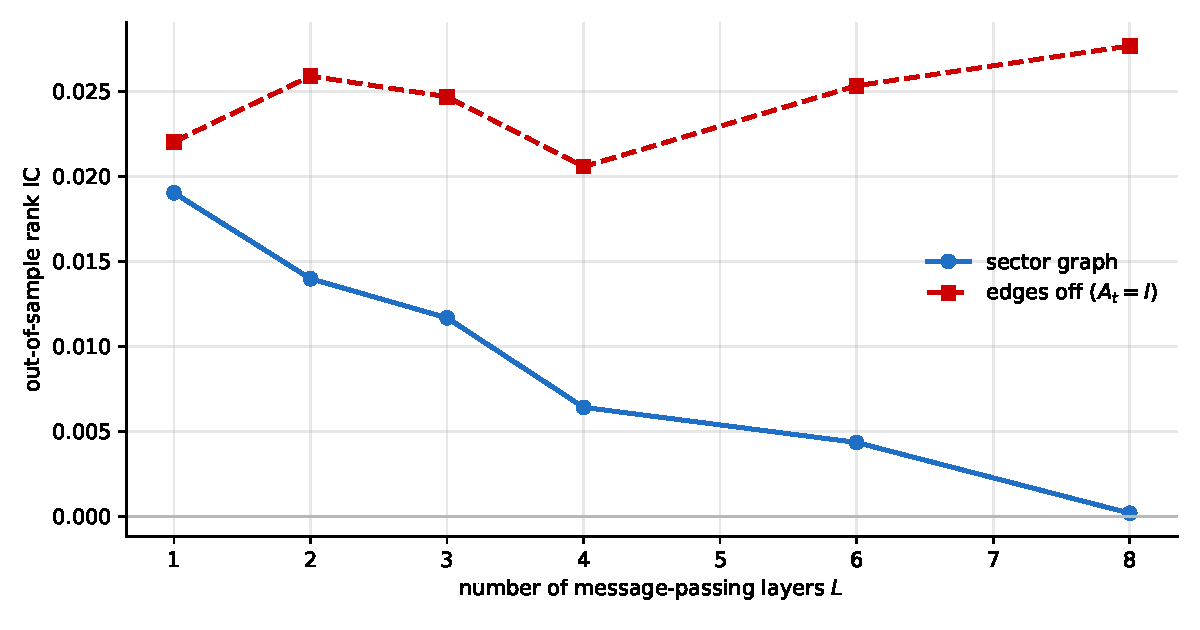
\includegraphics[width=0.7\linewidth]{files/figure_9_1_depth-480aa7d0e1070b2514e7ee060a8c2b41.pdf}
\caption[]{The depth sweep with and without the sector edges. With the edges the out-of-sample rank IC decays to essentially zero as layers are added; with the adjacency removed the same architecture holds its rank IC at every depth.}
\label{fig-gnn-depth}
\end{figure}

\paragraph{Benchmarking against the graph-free control and LightGBM}\label{sec_gnn_bench}

We now refit each model annually on an expanding window, under five seeds, and collect its monthly rank IC. The snapshots are built once and sliced by year, and gradient boosting is refitted on the same windows.

\begin{verbatim}
import lightgbm as lgb
all_snaps = snapshots(panel)                               # build once, then slice by year
OOS = list(range(2015, 2027))
def split(year):
    return ([s for s in all_snaps if s[0].year < year],
            [s for s in all_snaps if s[0].year == year])
def walk_forward(build, seed):                             # refit each year, concatenate monthly ICs
    return pd.concat([ic_series(fit_gnn(build, tr, seed=seed), te)
                      for tr, te in (split(y) for y in OOS)]).sort_index()

series = {'sector graph': [], 'edges off': []}             # five monthly IC series per model
for sd in [0, 1, 2, 3, 4]:
    series['sector graph'].append(walk_forward(lambda: DeepGCN(K, 32, 2), sd))
    series['edges off'].append(walk_forward(lambda: DeepGCN_NoGraph(K, 32, 2), sd))

lgb_ic = {}                                                # LightGBM on the same windows (float32 path)
for y in OOS:
    tr, te = split(y)
    Xtr, ytr = np.vstack([s[1].numpy() for s in tr]), np.concatenate([s[2].numpy() for s in tr])
    m = lgb.LGBMRegressor(n_estimators=300, num_leaves=31, learning_rate=0.05,
                          random_state=SEED, verbose=-1, n_jobs=1, deterministic=True).fit(Xtr, ytr)
    for dt, X, _, sec, raw in te:
        ic = spearmanr(m.predict(X.numpy()), raw).statistic
        if not np.isnan(ic): lgb_ic[dt] = ic
lgb_s = pd.Series(lgb_ic).sort_index()
mseries = {k: pd.concat(v, axis=1).mean(axis=1).sort_index() for k, v in series.items()}
print(f"5-seed mean rank IC   sector graph {mseries['sector graph'].mean():.4f}   "
      f"edges off {mseries['edges off'].mean():.4f}   LightGBM {lgb_s.mean():.4f}")
\end{verbatim}

\begin{verbatim}
C:\Users\tguid\miniconda3\envs\futures_dl\Lib\site-packages\sklearn\utils\validation.py:2691: UserWarning: X does not have valid feature names, but LGBMRegressor was fitted with feature names
  warnings.warn(
C:\Users\tguid\miniconda3\envs\futures_dl\Lib\site-packages\sklearn\utils\validation.py:2691: UserWarning: X does not have valid feature names, but LGBMRegressor was fitted with feature names
  warnings.warn(
C:\Users\tguid\miniconda3\envs\futures_dl\Lib\site-packages\sklearn\utils\validation.py:2691: UserWarning: X does not have valid feature names, but LGBMRegressor was fitted with feature names
  warnings.warn(
C:\Users\tguid\miniconda3\envs\futures_dl\Lib\site-packages\sklearn\utils\validation.py:2691: UserWarning: X does not have valid feature names, but LGBMRegressor was fitted with feature names
  warnings.warn(
C:\Users\tguid\miniconda3\envs\futures_dl\Lib\site-packages\sklearn\utils\validation.py:2691: UserWarning: X does not have valid feature names, but LGBMRegressor was fitted with feature names
  warnings.warn(
C:\Users\tguid\miniconda3\envs\futures_dl\Lib\site-packages\sklearn\utils\validation.py:2691: UserWarning: X does not have valid feature names, but LGBMRegressor was fitted with feature names
  warnings.warn(
C:\Users\tguid\miniconda3\envs\futures_dl\Lib\site-packages\sklearn\utils\validation.py:2691: UserWarning: X does not have valid feature names, but LGBMRegressor was fitted with feature names
  warnings.warn(
C:\Users\tguid\miniconda3\envs\futures_dl\Lib\site-packages\sklearn\utils\validation.py:2691: UserWarning: X does not have valid feature names, but LGBMRegressor was fitted with feature names
  warnings.warn(
C:\Users\tguid\miniconda3\envs\futures_dl\Lib\site-packages\sklearn\utils\validation.py:2691: UserWarning: X does not have valid feature names, but LGBMRegressor was fitted with feature names
  warnings.warn(
\end{verbatim}

\begin{verbatim}
C:\Users\tguid\miniconda3\envs\futures_dl\Lib\site-packages\sklearn\utils\validation.py:2691: UserWarning: X does not have valid feature names, but LGBMRegressor was fitted with feature names
  warnings.warn(
C:\Users\tguid\miniconda3\envs\futures_dl\Lib\site-packages\sklearn\utils\validation.py:2691: UserWarning: X does not have valid feature names, but LGBMRegressor was fitted with feature names
  warnings.warn(
C:\Users\tguid\miniconda3\envs\futures_dl\Lib\site-packages\sklearn\utils\validation.py:2691: UserWarning: X does not have valid feature names, but LGBMRegressor was fitted with feature names
  warnings.warn(
\end{verbatim}

\begin{verbatim}
C:\Users\tguid\miniconda3\envs\futures_dl\Lib\site-packages\sklearn\utils\validation.py:2691: UserWarning: X does not have valid feature names, but LGBMRegressor was fitted with feature names
  warnings.warn(
C:\Users\tguid\miniconda3\envs\futures_dl\Lib\site-packages\sklearn\utils\validation.py:2691: UserWarning: X does not have valid feature names, but LGBMRegressor was fitted with feature names
  warnings.warn(
C:\Users\tguid\miniconda3\envs\futures_dl\Lib\site-packages\sklearn\utils\validation.py:2691: UserWarning: X does not have valid feature names, but LGBMRegressor was fitted with feature names
  warnings.warn(
C:\Users\tguid\miniconda3\envs\futures_dl\Lib\site-packages\sklearn\utils\validation.py:2691: UserWarning: X does not have valid feature names, but LGBMRegressor was fitted with feature names
  warnings.warn(
C:\Users\tguid\miniconda3\envs\futures_dl\Lib\site-packages\sklearn\utils\validation.py:2691: UserWarning: X does not have valid feature names, but LGBMRegressor was fitted with feature names
  warnings.warn(
C:\Users\tguid\miniconda3\envs\futures_dl\Lib\site-packages\sklearn\utils\validation.py:2691: UserWarning: X does not have valid feature names, but LGBMRegressor was fitted with feature names
  warnings.warn(
C:\Users\tguid\miniconda3\envs\futures_dl\Lib\site-packages\sklearn\utils\validation.py:2691: UserWarning: X does not have valid feature names, but LGBMRegressor was fitted with feature names
  warnings.warn(
C:\Users\tguid\miniconda3\envs\futures_dl\Lib\site-packages\sklearn\utils\validation.py:2691: UserWarning: X does not have valid feature names, but LGBMRegressor was fitted with feature names
  warnings.warn(
C:\Users\tguid\miniconda3\envs\futures_dl\Lib\site-packages\sklearn\utils\validation.py:2691: UserWarning: X does not have valid feature names, but LGBMRegressor was fitted with feature names
  warnings.warn(
\end{verbatim}

\begin{verbatim}
C:\Users\tguid\miniconda3\envs\futures_dl\Lib\site-packages\sklearn\utils\validation.py:2691: UserWarning: X does not have valid feature names, but LGBMRegressor was fitted with feature names
  warnings.warn(
C:\Users\tguid\miniconda3\envs\futures_dl\Lib\site-packages\sklearn\utils\validation.py:2691: UserWarning: X does not have valid feature names, but LGBMRegressor was fitted with feature names
  warnings.warn(
C:\Users\tguid\miniconda3\envs\futures_dl\Lib\site-packages\sklearn\utils\validation.py:2691: UserWarning: X does not have valid feature names, but LGBMRegressor was fitted with feature names
  warnings.warn(
\end{verbatim}

\begin{verbatim}
C:\Users\tguid\miniconda3\envs\futures_dl\Lib\site-packages\sklearn\utils\validation.py:2691: UserWarning: X does not have valid feature names, but LGBMRegressor was fitted with feature names
  warnings.warn(
C:\Users\tguid\miniconda3\envs\futures_dl\Lib\site-packages\sklearn\utils\validation.py:2691: UserWarning: X does not have valid feature names, but LGBMRegressor was fitted with feature names
  warnings.warn(
C:\Users\tguid\miniconda3\envs\futures_dl\Lib\site-packages\sklearn\utils\validation.py:2691: UserWarning: X does not have valid feature names, but LGBMRegressor was fitted with feature names
  warnings.warn(
C:\Users\tguid\miniconda3\envs\futures_dl\Lib\site-packages\sklearn\utils\validation.py:2691: UserWarning: X does not have valid feature names, but LGBMRegressor was fitted with feature names
  warnings.warn(
C:\Users\tguid\miniconda3\envs\futures_dl\Lib\site-packages\sklearn\utils\validation.py:2691: UserWarning: X does not have valid feature names, but LGBMRegressor was fitted with feature names
  warnings.warn(
C:\Users\tguid\miniconda3\envs\futures_dl\Lib\site-packages\sklearn\utils\validation.py:2691: UserWarning: X does not have valid feature names, but LGBMRegressor was fitted with feature names
  warnings.warn(
C:\Users\tguid\miniconda3\envs\futures_dl\Lib\site-packages\sklearn\utils\validation.py:2691: UserWarning: X does not have valid feature names, but LGBMRegressor was fitted with feature names
  warnings.warn(
C:\Users\tguid\miniconda3\envs\futures_dl\Lib\site-packages\sklearn\utils\validation.py:2691: UserWarning: X does not have valid feature names, but LGBMRegressor was fitted with feature names
  warnings.warn(
\end{verbatim}

\begin{verbatim}
C:\Users\tguid\miniconda3\envs\futures_dl\Lib\site-packages\sklearn\utils\validation.py:2691: UserWarning: X does not have valid feature names, but LGBMRegressor was fitted with feature names
  warnings.warn(
C:\Users\tguid\miniconda3\envs\futures_dl\Lib\site-packages\sklearn\utils\validation.py:2691: UserWarning: X does not have valid feature names, but LGBMRegressor was fitted with feature names
  warnings.warn(
C:\Users\tguid\miniconda3\envs\futures_dl\Lib\site-packages\sklearn\utils\validation.py:2691: UserWarning: X does not have valid feature names, but LGBMRegressor was fitted with feature names
  warnings.warn(
C:\Users\tguid\miniconda3\envs\futures_dl\Lib\site-packages\sklearn\utils\validation.py:2691: UserWarning: X does not have valid feature names, but LGBMRegressor was fitted with feature names
  warnings.warn(
\end{verbatim}

\begin{verbatim}
C:\Users\tguid\miniconda3\envs\futures_dl\Lib\site-packages\sklearn\utils\validation.py:2691: UserWarning: X does not have valid feature names, but LGBMRegressor was fitted with feature names
  warnings.warn(
C:\Users\tguid\miniconda3\envs\futures_dl\Lib\site-packages\sklearn\utils\validation.py:2691: UserWarning: X does not have valid feature names, but LGBMRegressor was fitted with feature names
  warnings.warn(
C:\Users\tguid\miniconda3\envs\futures_dl\Lib\site-packages\sklearn\utils\validation.py:2691: UserWarning: X does not have valid feature names, but LGBMRegressor was fitted with feature names
  warnings.warn(
C:\Users\tguid\miniconda3\envs\futures_dl\Lib\site-packages\sklearn\utils\validation.py:2691: UserWarning: X does not have valid feature names, but LGBMRegressor was fitted with feature names
  warnings.warn(
C:\Users\tguid\miniconda3\envs\futures_dl\Lib\site-packages\sklearn\utils\validation.py:2691: UserWarning: X does not have valid feature names, but LGBMRegressor was fitted with feature names
  warnings.warn(
C:\Users\tguid\miniconda3\envs\futures_dl\Lib\site-packages\sklearn\utils\validation.py:2691: UserWarning: X does not have valid feature names, but LGBMRegressor was fitted with feature names
  warnings.warn(
C:\Users\tguid\miniconda3\envs\futures_dl\Lib\site-packages\sklearn\utils\validation.py:2691: UserWarning: X does not have valid feature names, but LGBMRegressor was fitted with feature names
  warnings.warn(
C:\Users\tguid\miniconda3\envs\futures_dl\Lib\site-packages\sklearn\utils\validation.py:2691: UserWarning: X does not have valid feature names, but LGBMRegressor was fitted with feature names
  warnings.warn(
C:\Users\tguid\miniconda3\envs\futures_dl\Lib\site-packages\sklearn\utils\validation.py:2691: UserWarning: X does not have valid feature names, but LGBMRegressor was fitted with feature names
  warnings.warn(
\end{verbatim}

\begin{verbatim}
C:\Users\tguid\miniconda3\envs\futures_dl\Lib\site-packages\sklearn\utils\validation.py:2691: UserWarning: X does not have valid feature names, but LGBMRegressor was fitted with feature names
  warnings.warn(
C:\Users\tguid\miniconda3\envs\futures_dl\Lib\site-packages\sklearn\utils\validation.py:2691: UserWarning: X does not have valid feature names, but LGBMRegressor was fitted with feature names
  warnings.warn(
C:\Users\tguid\miniconda3\envs\futures_dl\Lib\site-packages\sklearn\utils\validation.py:2691: UserWarning: X does not have valid feature names, but LGBMRegressor was fitted with feature names
  warnings.warn(
\end{verbatim}

\begin{verbatim}
C:\Users\tguid\miniconda3\envs\futures_dl\Lib\site-packages\sklearn\utils\validation.py:2691: UserWarning: X does not have valid feature names, but LGBMRegressor was fitted with feature names
  warnings.warn(
C:\Users\tguid\miniconda3\envs\futures_dl\Lib\site-packages\sklearn\utils\validation.py:2691: UserWarning: X does not have valid feature names, but LGBMRegressor was fitted with feature names
  warnings.warn(
C:\Users\tguid\miniconda3\envs\futures_dl\Lib\site-packages\sklearn\utils\validation.py:2691: UserWarning: X does not have valid feature names, but LGBMRegressor was fitted with feature names
  warnings.warn(
C:\Users\tguid\miniconda3\envs\futures_dl\Lib\site-packages\sklearn\utils\validation.py:2691: UserWarning: X does not have valid feature names, but LGBMRegressor was fitted with feature names
  warnings.warn(
C:\Users\tguid\miniconda3\envs\futures_dl\Lib\site-packages\sklearn\utils\validation.py:2691: UserWarning: X does not have valid feature names, but LGBMRegressor was fitted with feature names
  warnings.warn(
C:\Users\tguid\miniconda3\envs\futures_dl\Lib\site-packages\sklearn\utils\validation.py:2691: UserWarning: X does not have valid feature names, but LGBMRegressor was fitted with feature names
  warnings.warn(
C:\Users\tguid\miniconda3\envs\futures_dl\Lib\site-packages\sklearn\utils\validation.py:2691: UserWarning: X does not have valid feature names, but LGBMRegressor was fitted with feature names
  warnings.warn(
C:\Users\tguid\miniconda3\envs\futures_dl\Lib\site-packages\sklearn\utils\validation.py:2691: UserWarning: X does not have valid feature names, but LGBMRegressor was fitted with feature names
  warnings.warn(
C:\Users\tguid\miniconda3\envs\futures_dl\Lib\site-packages\sklearn\utils\validation.py:2691: UserWarning: X does not have valid feature names, but LGBMRegressor was fitted with feature names
  warnings.warn(
C:\Users\tguid\miniconda3\envs\futures_dl\Lib\site-packages\sklearn\utils\validation.py:2691: UserWarning: X does not have valid feature names, but LGBMRegressor was fitted with feature names
  warnings.warn(
\end{verbatim}

\begin{verbatim}
C:\Users\tguid\miniconda3\envs\futures_dl\Lib\site-packages\sklearn\utils\validation.py:2691: UserWarning: X does not have valid feature names, but LGBMRegressor was fitted with feature names
  warnings.warn(
C:\Users\tguid\miniconda3\envs\futures_dl\Lib\site-packages\sklearn\utils\validation.py:2691: UserWarning: X does not have valid feature names, but LGBMRegressor was fitted with feature names
  warnings.warn(
\end{verbatim}

\begin{verbatim}
C:\Users\tguid\miniconda3\envs\futures_dl\Lib\site-packages\sklearn\utils\validation.py:2691: UserWarning: X does not have valid feature names, but LGBMRegressor was fitted with feature names
  warnings.warn(
C:\Users\tguid\miniconda3\envs\futures_dl\Lib\site-packages\sklearn\utils\validation.py:2691: UserWarning: X does not have valid feature names, but LGBMRegressor was fitted with feature names
  warnings.warn(
C:\Users\tguid\miniconda3\envs\futures_dl\Lib\site-packages\sklearn\utils\validation.py:2691: UserWarning: X does not have valid feature names, but LGBMRegressor was fitted with feature names
  warnings.warn(
C:\Users\tguid\miniconda3\envs\futures_dl\Lib\site-packages\sklearn\utils\validation.py:2691: UserWarning: X does not have valid feature names, but LGBMRegressor was fitted with feature names
  warnings.warn(
C:\Users\tguid\miniconda3\envs\futures_dl\Lib\site-packages\sklearn\utils\validation.py:2691: UserWarning: X does not have valid feature names, but LGBMRegressor was fitted with feature names
  warnings.warn(
C:\Users\tguid\miniconda3\envs\futures_dl\Lib\site-packages\sklearn\utils\validation.py:2691: UserWarning: X does not have valid feature names, but LGBMRegressor was fitted with feature names
  warnings.warn(
C:\Users\tguid\miniconda3\envs\futures_dl\Lib\site-packages\sklearn\utils\validation.py:2691: UserWarning: X does not have valid feature names, but LGBMRegressor was fitted with feature names
  warnings.warn(
C:\Users\tguid\miniconda3\envs\futures_dl\Lib\site-packages\sklearn\utils\validation.py:2691: UserWarning: X does not have valid feature names, but LGBMRegressor was fitted with feature names
  warnings.warn(
C:\Users\tguid\miniconda3\envs\futures_dl\Lib\site-packages\sklearn\utils\validation.py:2691: UserWarning: X does not have valid feature names, but LGBMRegressor was fitted with feature names
  warnings.warn(
\end{verbatim}

\begin{verbatim}
C:\Users\tguid\miniconda3\envs\futures_dl\Lib\site-packages\sklearn\utils\validation.py:2691: UserWarning: X does not have valid feature names, but LGBMRegressor was fitted with feature names
  warnings.warn(
C:\Users\tguid\miniconda3\envs\futures_dl\Lib\site-packages\sklearn\utils\validation.py:2691: UserWarning: X does not have valid feature names, but LGBMRegressor was fitted with feature names
  warnings.warn(
C:\Users\tguid\miniconda3\envs\futures_dl\Lib\site-packages\sklearn\utils\validation.py:2691: UserWarning: X does not have valid feature names, but LGBMRegressor was fitted with feature names
  warnings.warn(
\end{verbatim}

\begin{verbatim}
C:\Users\tguid\miniconda3\envs\futures_dl\Lib\site-packages\sklearn\utils\validation.py:2691: UserWarning: X does not have valid feature names, but LGBMRegressor was fitted with feature names
  warnings.warn(
C:\Users\tguid\miniconda3\envs\futures_dl\Lib\site-packages\sklearn\utils\validation.py:2691: UserWarning: X does not have valid feature names, but LGBMRegressor was fitted with feature names
  warnings.warn(
C:\Users\tguid\miniconda3\envs\futures_dl\Lib\site-packages\sklearn\utils\validation.py:2691: UserWarning: X does not have valid feature names, but LGBMRegressor was fitted with feature names
  warnings.warn(
C:\Users\tguid\miniconda3\envs\futures_dl\Lib\site-packages\sklearn\utils\validation.py:2691: UserWarning: X does not have valid feature names, but LGBMRegressor was fitted with feature names
  warnings.warn(
C:\Users\tguid\miniconda3\envs\futures_dl\Lib\site-packages\sklearn\utils\validation.py:2691: UserWarning: X does not have valid feature names, but LGBMRegressor was fitted with feature names
  warnings.warn(
C:\Users\tguid\miniconda3\envs\futures_dl\Lib\site-packages\sklearn\utils\validation.py:2691: UserWarning: X does not have valid feature names, but LGBMRegressor was fitted with feature names
  warnings.warn(
C:\Users\tguid\miniconda3\envs\futures_dl\Lib\site-packages\sklearn\utils\validation.py:2691: UserWarning: X does not have valid feature names, but LGBMRegressor was fitted with feature names
  warnings.warn(
C:\Users\tguid\miniconda3\envs\futures_dl\Lib\site-packages\sklearn\utils\validation.py:2691: UserWarning: X does not have valid feature names, but LGBMRegressor was fitted with feature names
  warnings.warn(
C:\Users\tguid\miniconda3\envs\futures_dl\Lib\site-packages\sklearn\utils\validation.py:2691: UserWarning: X does not have valid feature names, but LGBMRegressor was fitted with feature names
  warnings.warn(
\end{verbatim}

\begin{verbatim}
C:\Users\tguid\miniconda3\envs\futures_dl\Lib\site-packages\sklearn\utils\validation.py:2691: UserWarning: X does not have valid feature names, but LGBMRegressor was fitted with feature names
  warnings.warn(
C:\Users\tguid\miniconda3\envs\futures_dl\Lib\site-packages\sklearn\utils\validation.py:2691: UserWarning: X does not have valid feature names, but LGBMRegressor was fitted with feature names
  warnings.warn(
C:\Users\tguid\miniconda3\envs\futures_dl\Lib\site-packages\sklearn\utils\validation.py:2691: UserWarning: X does not have valid feature names, but LGBMRegressor was fitted with feature names
  warnings.warn(
\end{verbatim}

\begin{verbatim}
C:\Users\tguid\miniconda3\envs\futures_dl\Lib\site-packages\sklearn\utils\validation.py:2691: UserWarning: X does not have valid feature names, but LGBMRegressor was fitted with feature names
  warnings.warn(
C:\Users\tguid\miniconda3\envs\futures_dl\Lib\site-packages\sklearn\utils\validation.py:2691: UserWarning: X does not have valid feature names, but LGBMRegressor was fitted with feature names
  warnings.warn(
C:\Users\tguid\miniconda3\envs\futures_dl\Lib\site-packages\sklearn\utils\validation.py:2691: UserWarning: X does not have valid feature names, but LGBMRegressor was fitted with feature names
  warnings.warn(
C:\Users\tguid\miniconda3\envs\futures_dl\Lib\site-packages\sklearn\utils\validation.py:2691: UserWarning: X does not have valid feature names, but LGBMRegressor was fitted with feature names
  warnings.warn(
C:\Users\tguid\miniconda3\envs\futures_dl\Lib\site-packages\sklearn\utils\validation.py:2691: UserWarning: X does not have valid feature names, but LGBMRegressor was fitted with feature names
  warnings.warn(
C:\Users\tguid\miniconda3\envs\futures_dl\Lib\site-packages\sklearn\utils\validation.py:2691: UserWarning: X does not have valid feature names, but LGBMRegressor was fitted with feature names
  warnings.warn(
C:\Users\tguid\miniconda3\envs\futures_dl\Lib\site-packages\sklearn\utils\validation.py:2691: UserWarning: X does not have valid feature names, but LGBMRegressor was fitted with feature names
  warnings.warn(
C:\Users\tguid\miniconda3\envs\futures_dl\Lib\site-packages\sklearn\utils\validation.py:2691: UserWarning: X does not have valid feature names, but LGBMRegressor was fitted with feature names
  warnings.warn(
C:\Users\tguid\miniconda3\envs\futures_dl\Lib\site-packages\sklearn\utils\validation.py:2691: UserWarning: X does not have valid feature names, but LGBMRegressor was fitted with feature names
  warnings.warn(
\end{verbatim}

\begin{verbatim}
C:\Users\tguid\miniconda3\envs\futures_dl\Lib\site-packages\sklearn\utils\validation.py:2691: UserWarning: X does not have valid feature names, but LGBMRegressor was fitted with feature names
  warnings.warn(
C:\Users\tguid\miniconda3\envs\futures_dl\Lib\site-packages\sklearn\utils\validation.py:2691: UserWarning: X does not have valid feature names, but LGBMRegressor was fitted with feature names
  warnings.warn(
C:\Users\tguid\miniconda3\envs\futures_dl\Lib\site-packages\sklearn\utils\validation.py:2691: UserWarning: X does not have valid feature names, but LGBMRegressor was fitted with feature names
  warnings.warn(
\end{verbatim}

\begin{verbatim}
C:\Users\tguid\miniconda3\envs\futures_dl\Lib\site-packages\sklearn\utils\validation.py:2691: UserWarning: X does not have valid feature names, but LGBMRegressor was fitted with feature names
  warnings.warn(
C:\Users\tguid\miniconda3\envs\futures_dl\Lib\site-packages\sklearn\utils\validation.py:2691: UserWarning: X does not have valid feature names, but LGBMRegressor was fitted with feature names
  warnings.warn(
C:\Users\tguid\miniconda3\envs\futures_dl\Lib\site-packages\sklearn\utils\validation.py:2691: UserWarning: X does not have valid feature names, but LGBMRegressor was fitted with feature names
  warnings.warn(
C:\Users\tguid\miniconda3\envs\futures_dl\Lib\site-packages\sklearn\utils\validation.py:2691: UserWarning: X does not have valid feature names, but LGBMRegressor was fitted with feature names
  warnings.warn(
C:\Users\tguid\miniconda3\envs\futures_dl\Lib\site-packages\sklearn\utils\validation.py:2691: UserWarning: X does not have valid feature names, but LGBMRegressor was fitted with feature names
  warnings.warn(
C:\Users\tguid\miniconda3\envs\futures_dl\Lib\site-packages\sklearn\utils\validation.py:2691: UserWarning: X does not have valid feature names, but LGBMRegressor was fitted with feature names
  warnings.warn(
C:\Users\tguid\miniconda3\envs\futures_dl\Lib\site-packages\sklearn\utils\validation.py:2691: UserWarning: X does not have valid feature names, but LGBMRegressor was fitted with feature names
  warnings.warn(
C:\Users\tguid\miniconda3\envs\futures_dl\Lib\site-packages\sklearn\utils\validation.py:2691: UserWarning: X does not have valid feature names, but LGBMRegressor was fitted with feature names
  warnings.warn(
C:\Users\tguid\miniconda3\envs\futures_dl\Lib\site-packages\sklearn\utils\validation.py:2691: UserWarning: X does not have valid feature names, but LGBMRegressor was fitted with feature names
  warnings.warn(
\end{verbatim}

\begin{verbatim}
C:\Users\tguid\miniconda3\envs\futures_dl\Lib\site-packages\sklearn\utils\validation.py:2691: UserWarning: X does not have valid feature names, but LGBMRegressor was fitted with feature names
  warnings.warn(
C:\Users\tguid\miniconda3\envs\futures_dl\Lib\site-packages\sklearn\utils\validation.py:2691: UserWarning: X does not have valid feature names, but LGBMRegressor was fitted with feature names
  warnings.warn(
C:\Users\tguid\miniconda3\envs\futures_dl\Lib\site-packages\sklearn\utils\validation.py:2691: UserWarning: X does not have valid feature names, but LGBMRegressor was fitted with feature names
  warnings.warn(
\end{verbatim}

\begin{verbatim}
C:\Users\tguid\miniconda3\envs\futures_dl\Lib\site-packages\sklearn\utils\validation.py:2691: UserWarning: X does not have valid feature names, but LGBMRegressor was fitted with feature names
  warnings.warn(
C:\Users\tguid\miniconda3\envs\futures_dl\Lib\site-packages\sklearn\utils\validation.py:2691: UserWarning: X does not have valid feature names, but LGBMRegressor was fitted with feature names
  warnings.warn(
C:\Users\tguid\miniconda3\envs\futures_dl\Lib\site-packages\sklearn\utils\validation.py:2691: UserWarning: X does not have valid feature names, but LGBMRegressor was fitted with feature names
  warnings.warn(
C:\Users\tguid\miniconda3\envs\futures_dl\Lib\site-packages\sklearn\utils\validation.py:2691: UserWarning: X does not have valid feature names, but LGBMRegressor was fitted with feature names
  warnings.warn(
C:\Users\tguid\miniconda3\envs\futures_dl\Lib\site-packages\sklearn\utils\validation.py:2691: UserWarning: X does not have valid feature names, but LGBMRegressor was fitted with feature names
  warnings.warn(
C:\Users\tguid\miniconda3\envs\futures_dl\Lib\site-packages\sklearn\utils\validation.py:2691: UserWarning: X does not have valid feature names, but LGBMRegressor was fitted with feature names
  warnings.warn(
C:\Users\tguid\miniconda3\envs\futures_dl\Lib\site-packages\sklearn\utils\validation.py:2691: UserWarning: X does not have valid feature names, but LGBMRegressor was fitted with feature names
  warnings.warn(
C:\Users\tguid\miniconda3\envs\futures_dl\Lib\site-packages\sklearn\utils\validation.py:2691: UserWarning: X does not have valid feature names, but LGBMRegressor was fitted with feature names
  warnings.warn(
C:\Users\tguid\miniconda3\envs\futures_dl\Lib\site-packages\sklearn\utils\validation.py:2691: UserWarning: X does not have valid feature names, but LGBMRegressor was fitted with feature names
  warnings.warn(
\end{verbatim}

\begin{verbatim}
C:\Users\tguid\miniconda3\envs\futures_dl\Lib\site-packages\sklearn\utils\validation.py:2691: UserWarning: X does not have valid feature names, but LGBMRegressor was fitted with feature names
  warnings.warn(
C:\Users\tguid\miniconda3\envs\futures_dl\Lib\site-packages\sklearn\utils\validation.py:2691: UserWarning: X does not have valid feature names, but LGBMRegressor was fitted with feature names
  warnings.warn(
C:\Users\tguid\miniconda3\envs\futures_dl\Lib\site-packages\sklearn\utils\validation.py:2691: UserWarning: X does not have valid feature names, but LGBMRegressor was fitted with feature names
  warnings.warn(
\end{verbatim}

\begin{verbatim}
C:\Users\tguid\miniconda3\envs\futures_dl\Lib\site-packages\sklearn\utils\validation.py:2691: UserWarning: X does not have valid feature names, but LGBMRegressor was fitted with feature names
  warnings.warn(
C:\Users\tguid\miniconda3\envs\futures_dl\Lib\site-packages\sklearn\utils\validation.py:2691: UserWarning: X does not have valid feature names, but LGBMRegressor was fitted with feature names
  warnings.warn(
C:\Users\tguid\miniconda3\envs\futures_dl\Lib\site-packages\sklearn\utils\validation.py:2691: UserWarning: X does not have valid feature names, but LGBMRegressor was fitted with feature names
  warnings.warn(
C:\Users\tguid\miniconda3\envs\futures_dl\Lib\site-packages\sklearn\utils\validation.py:2691: UserWarning: X does not have valid feature names, but LGBMRegressor was fitted with feature names
  warnings.warn(
C:\Users\tguid\miniconda3\envs\futures_dl\Lib\site-packages\sklearn\utils\validation.py:2691: UserWarning: X does not have valid feature names, but LGBMRegressor was fitted with feature names
  warnings.warn(
C:\Users\tguid\miniconda3\envs\futures_dl\Lib\site-packages\sklearn\utils\validation.py:2691: UserWarning: X does not have valid feature names, but LGBMRegressor was fitted with feature names
  warnings.warn(
C:\Users\tguid\miniconda3\envs\futures_dl\Lib\site-packages\sklearn\utils\validation.py:2691: UserWarning: X does not have valid feature names, but LGBMRegressor was fitted with feature names
  warnings.warn(
C:\Users\tguid\miniconda3\envs\futures_dl\Lib\site-packages\sklearn\utils\validation.py:2691: UserWarning: X does not have valid feature names, but LGBMRegressor was fitted with feature names
  warnings.warn(
\end{verbatim}

\begin{verbatim}
C:\Users\tguid\miniconda3\envs\futures_dl\Lib\site-packages\sklearn\utils\validation.py:2691: UserWarning: X does not have valid feature names, but LGBMRegressor was fitted with feature names
  warnings.warn(
C:\Users\tguid\miniconda3\envs\futures_dl\Lib\site-packages\sklearn\utils\validation.py:2691: UserWarning: X does not have valid feature names, but LGBMRegressor was fitted with feature names
  warnings.warn(
C:\Users\tguid\miniconda3\envs\futures_dl\Lib\site-packages\sklearn\utils\validation.py:2691: UserWarning: X does not have valid feature names, but LGBMRegressor was fitted with feature names
  warnings.warn(
C:\Users\tguid\miniconda3\envs\futures_dl\Lib\site-packages\sklearn\utils\validation.py:2691: UserWarning: X does not have valid feature names, but LGBMRegressor was fitted with feature names
  warnings.warn(
\end{verbatim}

\begin{verbatim}
5-seed mean rank IC   sector graph 0.0216   edges off 0.0276   LightGBM 0.0346
\end{verbatim}

\begin{verbatim}
C:\Users\tguid\miniconda3\envs\futures_dl\Lib\site-packages\sklearn\utils\validation.py:2691: UserWarning: X does not have valid feature names, but LGBMRegressor was fitted with feature names
  warnings.warn(
C:\Users\tguid\miniconda3\envs\futures_dl\Lib\site-packages\sklearn\utils\validation.py:2691: UserWarning: X does not have valid feature names, but LGBMRegressor was fitted with feature names
  warnings.warn(
\end{verbatim}

Gradient boosting wins by a wide margin, at 0.0346, and the graph-free twin, at 0.0276, beats the sector-graph GCN, at 0.0216. The two neural models are the same architecture with the same 5,025 parameters, differing only in whether a firm's representation is averaged with its sector, and the version that ignores the edges forecasts better. Figure~\ref{fig-gnn-cumulative} accumulates the three monthly series, averaged across seeds: all three rise, so every model carries some signal, but the graph-free models accumulate faster and with fewer reversals.

\begin{verbatim}
fig, ax = plt.subplots(figsize=(10, 4))
for name, s, col in [('GCN (sector graph)', mseries['sector graph'], '#1f6fc4'),
                     ('edges off ($A_t=I$)', mseries['edges off'], '#cc0000'),
                     ('LightGBM', lgb_s, '#2e9e4f')]:
    ax.plot(s.index, s.cumsum().values, lw=1.7, color=col, label=f'{name}  (mean IC {s.mean():.3f})')
ax.axhline(0, color='#b8b8b8', lw=1); ax.set_ylabel('cumulative rank IC'); ax.set_xlabel('date')
ax.legend(frameon=False); ax.spines[['top', 'right']].set_visible(False); ax.grid(alpha=.3)
plt.tight_layout(); plt.savefig('images/figure_9_2_cumulative.png', dpi=150, bbox_inches='tight')
\end{verbatim}

\begin{figure}[!htbp]
\centering
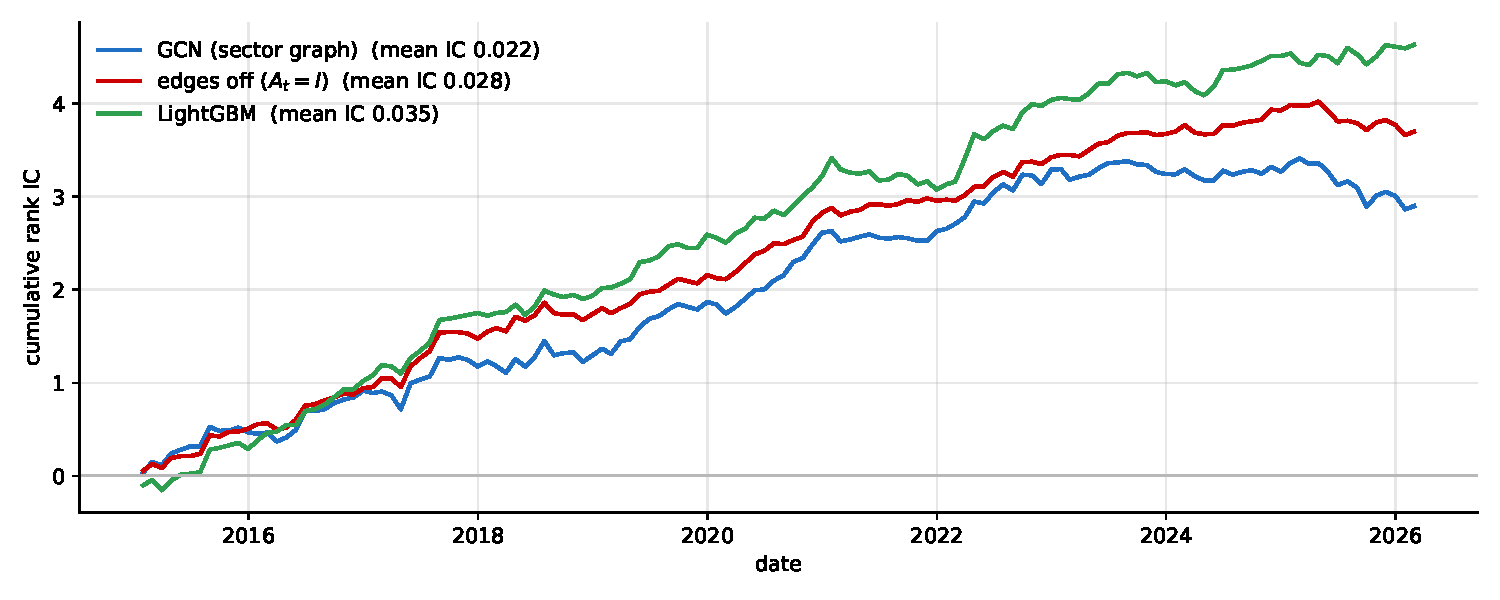
\includegraphics[width=0.7\linewidth]{files/figure_9_2_cumulativ-c0f6718ad81f94f0d78598b5cb722190.pdf}
\caption[]{Cumulative rank information coefficient over the testing period, averaged across five seeds. A rising line indicates a signal that keeps working; the vertical gaps are the cumulative cost of using the graph.}
\label{fig-gnn-cumulative}
\end{figure}

\begin{verbatim}
fig, ax = plt.subplots(figsize=(8, 4))
for i, (name, col) in enumerate([('sector graph', '#1f6fc4'), ('edges off', '#cc0000')]):
    vals = [s.mean() for s in series[name]]
    ax.scatter([i] * len(vals), vals, s=45, color=col, zorder=3)
    ax.hlines(np.mean(vals), i - 0.15, i + 0.15, color='black', lw=2, zorder=4)
ax.axhline(lgb_s.mean(), color='#2e9e4f', ls='--', lw=1.3, label=f'LightGBM ({lgb_s.mean():.4f})')
ax.set_xticks([0, 1]); ax.set_xticklabels(['GCN (sector graph)', 'edges off ($A_t=I$)'])
ax.set_ylabel('average rank IC'); ax.legend(frameon=False)
ax.spines[['top', 'right']].set_visible(False); ax.grid(alpha=.3, axis='y')
plt.tight_layout(); plt.savefig('images/figure_9_3_dispersion.png', dpi=150, bbox_inches='tight')
\end{verbatim}

\begin{figure}[!htbp]
\centering
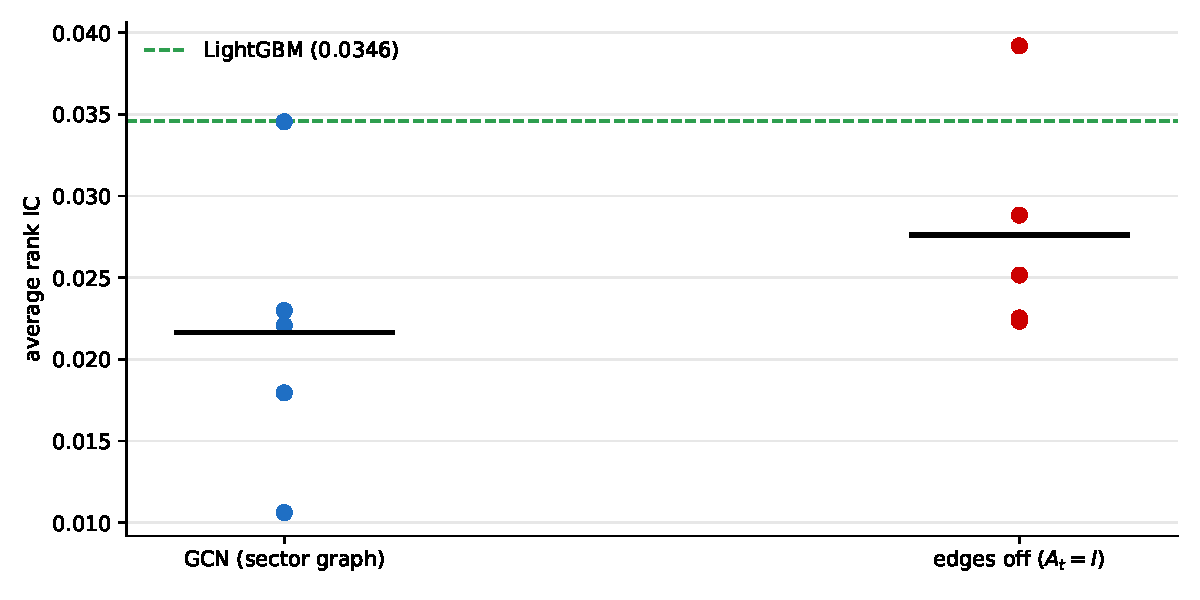
\includegraphics[width=0.7\linewidth]{files/figure_9_3_dispersio-fb54a2eb8780d0ddc05fe33f56526bf6.pdf}
\caption[]{Dispersion of the average rank IC across five random seeds for the sector-graph GCN and its edge-free twin, with the LightGBM benchmark dashed. The seed dispersion is comparable to the gap between the two models.}
\label{fig-gnn-dispersion}
\end{figure}

\paragraph{The ablation, and what survives the noise}\label{sec_gnn_survives}

Because both models are trained under the same five seeds, we difference the graph convolutional network against its own capacity-matched edge-free twin, seed by seed, which cancels the common component of initialisation noise. The twin is the identical class with its neighbourhood aggregation overridden to the identity, so it carries the same architecture and the same 5,025 parameters. Both the paired difference and a time-series test of the monthly gap come straight from the seed-by-seed information coefficients collected above.

\begin{verbatim}
diff = np.array([series['sector graph'][sd].mean() - series['edges off'][sd].mean()
                 for sd in range(5)])                       # paired within each seed
paired_t = diff.mean() / (diff.std(ddof=1) / np.sqrt(len(diff)))
def newey_west_t(x, lags=6):                                # HAC t-statistic for a mean
    x = np.asarray(x, float); n = len(x); e = x - x.mean(); s = e @ e / n
    for l in range(1, lags + 1):
        s += 2 * (1 - l / (lags + 1)) * (e[l:] @ e[:-l]) / n
    return x.mean() / np.sqrt(s / n)
monthly = (mseries['sector graph'] - mseries['edges off']).dropna()   # seed-averaged monthly gap
print(f'GCN minus edge-free twin: mean {diff.mean():+.4f}, '
      f'{int((diff > 0).sum())} of 5 seeds favour the graph, paired t = {paired_t:.2f}')
print(f'same gap over {len(monthly)} months: Newey-West t = {newey_west_t(monthly.values):.2f}')
\end{verbatim}

\begin{verbatim}
GCN minus edge-free twin: mean -0.0060, 0 of 5 seeds favour the graph, paired t = -3.98
same gap over 134 months: Newey-West t = -1.55
\end{verbatim}

TABLE 9.1 records the paired comparison. None of the five seeds favours the graph, and the paired t of -3.98 says the penalty is a stable property of the training procedure, not a lucky draw.

TABLE 9.1: Paired comparison of the graph convolutional network against its capacity-matched edge-free twin. The difference is computed within each seed and then averaged over five seeds. A positive difference would mean the edges add predictive content.

\bigskip\noindent
\begin{tabular}{p{\dimexpr 0.250\linewidth-2\tabcolsep}p{\dimexpr 0.250\linewidth-2\tabcolsep}p{\dimexpr 0.250\linewidth-2\tabcolsep}p{\dimexpr 0.250\linewidth-2\tabcolsep}}
\toprule
Comparison & Mean difference in rank IC & Seeds favouring the graph & Paired t \\
\hline
GCN minus its $\mathbf{A}_t=\mathbf{I}$ twin & -0.0060 & 0 of 5 & -3.98 \\
\bottomrule
\end{tabular}

\bigskip

The result is not special to the graph convolution. Repeating the same ablation for the attention and inductive variants of Section~\ref{sec_gnn_families}, each against its own edge-free twin, returns the same verdict: every architecture loses, with GraphSAGE penalised the least because its separate-then-concatenate design can most easily discount an uninformative neighbourhood, and GATv2 no better off because its attention gate still folds the neighbour average in.

The penalty should not, however, be overstated as a claim about this particular decade. The gap is robust across seeds, with a paired t of -3.98, yet the same monthly differences tested as a 134-month time series with Newey-West standard errors give t = -1.55, within the sampling noise a single backtest carries. Several further checks all point the same way. A range of alternative graphs, from correlation and nearest-neighbour constructions to an external corporate-relations graph, each lose to their own ablation, and the ones whose edges are the purest function of the node features do the most harm. Handing the graph to LightGBM as ordinary features rather than as a structure to propagate over changes nothing, since the 122 characteristics already express the grouping the edges encode. Replacing the averaging with a subtraction, the industry-neutralised peer-relative variant, removes the entire penalty but only recovers the graph-free performance. And net of twenty basis points of costs the graph turns over least yet still nets least. The verdict is therefore narrow and firm: on this panel the sector adjacency carries no incremental information a graph-free model does not already have, and the best a graph does is stop hurting.

\subsubsection{Other families of graph models}\label{sec_gnn_families}

The graph convolution is the simplest aggregator, and the family is larger. We survey the members most relevant to a cross-section of firms, isolating for each the one change it makes to the message-passing rule of equations (9.1) and (9.2), and keeping the treatment brief since none overturns the verdict of Section~\ref{sec_gnn_panel}.

\paragraph{Sampling and attention: GraphSAGE, GAT and GATv2}\label{sec_gnn_sage}

GraphSAGE (\cite{hamilton2017inductive}) departs from the graph convolution in the update step: instead of folding a node and its neighbours into a single weighted average before one linear map, as equation (9.2) does, it keeps the two in separate concatenated slots,

\begin{equation}
\label{eq_gnn_3}
\mathbf{o}_{t,n}^{(l+1)} = f^{(l)}\!\left( \mathbf{W}^{(l)} \left[\, \mathbf{o}_{t,n}^{(l)} \,\Big\|\, \underset{m \in \mathcal{N}(n)}{\mathrm{mean}}\ \mathbf{o}_{t,m}^{(l)} \,\right] \right)
\end{equation}

where $\|$ denotes concatenation and the neighbourhood $\mathcal{N}(n)$ is subsampled to a fixed size, so the cost per node does not grow with degree. Splitting the weight into the block acting on the node and the block acting on its neighbours, $\mathbf{W}^{(l)} = [\,\mathbf{W}^{(l)}_{\mathrm{self}}\ \ \mathbf{W}^{(l)}_{\mathrm{nbr}}\,]$, shows why the design matters here: the network can drive $\mathbf{W}^{(l)}_{\mathrm{nbr}}$ to zero and recover the graph-free map of Section~\ref{sec_gnn_ablation} exactly, discounting an uninformative neighbourhood rather than being forced to average it in. This is the mechanism behind GraphSAGE being the least penalised of the three architectures in Section~\ref{sec_gnn_survives}. Its inductive design, learning a function of a neighbourhood rather than a fixed per-node embedding, is also what lets a model trained on one month's graph apply to the next, whose node set differs.

Graph attention (\cite{velickovic2018graph}) keeps the aggregation of (9.2) but replaces its fixed, degree-based weights with learned, pair-specific ones,

\begin{equation}
\label{eq_gnn_4}
\mathbf{o}_{t,n}^{(l+1)} = f^{(l)}\!\Big( \sum_{m \in \mathcal{N}(n) \cup \{n\}} \alpha_{nm}\, \mathbf{W}^{(l)} \mathbf{o}_{t,m}^{(l)} \Big), \qquad \alpha_{nm} = \mathrm{softmax}_m\big(e_{nm}\big)
\end{equation}

with the score, in the original form, $e_{nm} = \mathrm{LeakyReLU}\big( \mathbf{a}'[\mathbf{W}\mathbf{o}_{t,n} \,\|\, \mathbf{W}\mathbf{o}_{t,m}] \big)$. One line of algebra exposes its flaw. Writing $\mathbf{a} = [\mathbf{a}_1 \,\|\, \mathbf{a}_2]$, the score is $\mathrm{LeakyReLU}\big(\mathbf{a}_1'\mathbf{W}\mathbf{o}_{t,n} + \mathbf{a}_2'\mathbf{W}\mathbf{o}_{t,m}\big)$; for a fixed query node $n$ the first term is constant across the neighbours $m$, and because LeakyReLU is monotone the neighbours are ranked by $\mathbf{a}_2'\mathbf{W}\mathbf{o}_{t,m}$ alone, an ordering that does not depend on $n$. Every node therefore attends to its neighbours in the same order, a static attention that cannot let a bank attend to one set of peers while a miner attends to another. \cite{brody2022attentive} correct this in GATv2 by moving the linear map and the nonlinearity, scoring with $e_{nm} = \mathbf{a}'\,\mathrm{LeakyReLU}\big(\mathbf{W}[\mathbf{o}_{t,n} \,\|\, \mathbf{o}_{t,m}]\big)$, which makes the score a universal approximator of the pair and the attention genuinely dynamic. On our panel GATv2's edges are as costly as the GCN's, and the added expressiveness buys nothing when the graph itself is uninformative.

\paragraph{Sum aggregation and typed edges: GIN and R-GCN}\label{sec_gnn_gin}

The graph isomorphism network of \cite{xu2019powerful} changes the aggregator in (9.1) from a mean to a sum, wrapped in a small multilayer perceptron with a tunable self-weight,

\begin{equation}
\label{eq_gnn_5}
\mathbf{o}_{t,n}^{(l+1)} = \mathrm{MLP}^{(l)}\!\Big( \big(1 + \epsilon^{(l)}\big)\,\mathbf{o}_{t,n}^{(l)} + \sum_{m \in \mathcal{N}(n)} \mathbf{o}_{t,m}^{(l)} \Big).
\end{equation}

The sum is injective on multisets where the mean is not: a neighbourhood $\{\mathbf{a}\}$ and a neighbourhood $\{\mathbf{a}, \mathbf{a}\}$ share a mean but differ in sum, so a mean aggregator cannot tell a node with one such neighbour from a node with two. This is what gives GIN the discriminative power of the Weisfeiler-Lehman graph isomorphism test. The distinction is largely moot here, as the authors themselves note: mean and sum coincide in power once node features are rich and rarely repeat, the situation of a cross-section described by 122 continuous characteristics.

When edges carry types, as in a knowledge graph of supplier, competitor and subsidiary relations, the relational GCN of \cite{schlichtkrull2018modeling} sums a separate transform over each relation,

\begin{equation}
\label{eq_gnn_6}
\mathbf{o}_{t,n}^{(l+1)} = f^{(l)}\!\Big( \mathbf{W}_0^{(l)}\mathbf{o}_{t,n}^{(l)} + \sum_{r \in \mathcal{R}} \sum_{m \in \mathcal{N}_r(n)} \frac{1}{c_{n,r}}\, \mathbf{W}_r^{(l)}\mathbf{o}_{t,m}^{(l)} \Big)
\end{equation}

where $\mathcal{N}_r(n)$ are the neighbours under relation $r$ and $c_{n,r}$ a normaliser; equation (9.2) is the single-relation special case. Because a distinct $\mathbf{W}_r^{(l)}$ per relation is expensive, the relations share a small set of $B$ basis matrices, $\mathbf{W}_r^{(l)} = \sum_{b=1}^{B} a_{rb}^{(l)}\mathbf{V}_b^{(l)}$, which controls the parameter count. It is the natural architecture for external corporate-relation graphs, none of which earned its edges on our data.

\paragraph{Temporal and spatio-temporal graphs}\label{sec_gnn_temporal}

A final family lets the graph, or the model acting on it, evolve, which a monthly panel with a changing node set invites. Where a static GNN applies the same weights at every date, EvolveGCN (\cite{pareja2020evolvegcn}) drives the weight matrix of a graph convolution with a recurrent network,

\begin{equation}
\label{eq_gnn_7}
\mathbf{W}_t^{(l)} = \mathrm{GRU}\big(\mathbf{W}_{t-1}^{(l)},\, \mathbf{H}_t^{(l)}\big)
\end{equation}

so equation (9.2) is applied at each date with weights that carry state across time rather than being refitted independently. The temporal graph attention of \cite{xu2020inductive} instead augments the attention score of (9.4) with a functional encoding of the elapsed time, weighting recent interactions more heavily, and PyTorch Geometric Temporal (\cite{rozemberczki2021pytorch}) makes both accessible. We do not pursue them, for the reason the static results make plain: there is little sense in letting a graph evolve until a static one has been shown to help, and on this panel none has.

\subsubsection{Interpretability}\label{sec_gnn_interp}

If a graph model did produce a useful signal, the natural question is which neighbours and which characteristics produced it. The literature on explaining graph networks, surveyed by \cite{yuan2023explainability}, is organised along three axes worth naming, because each determines what an explanation can and cannot claim. The first is local versus global: a local explanation accounts for a single prediction, one firm on one date, while a global explanation characterises the model's logic across the whole sample, such as the concept a hidden neuron responds to. The second is the instance-level explainer, which for one prediction returns a compact subgraph and a small set of features that suffice to reproduce it. The third, and the most consequential, is intrinsic versus post-hoc: an intrinsically interpretable model builds transparency into its architecture, whereas a post-hoc method probes an already-trained model from outside. A graph convolutional network is not intrinsically interpretable, and attention, the one component that looks as though it might be, is a weak substitute: the debate opened by \cite{jain2019attention} over whether attention weights are explanations is unresolved, and both \cite{ying2019gnnexplainer} and \cite{luo2020parameterized} find an attention baseline the weakest method at recovering structure known to have generated the label.

The standard post-hoc, instance-level tools are therefore the ones to reach for. GNNExplainer (\cite{ying2019gnnexplainer}) learns a soft mask over the edges and node features in a prediction's neighbourhood by maximising the mutual information between the masked input and the model's output. Writing $\mathbf{M}$ for the edge mask, $f$ for the trained network and $\hat{y}$ for its original prediction, this is equivalent to

\begin{equation}
\label{eq_gnn_8}
\min_{\mathbf{M}}\ \ell\big(\hat{y},\, f(\mathcal{G}_{\mathbf{M}})\big) + \lambda \lVert \mathbf{M} \rVert_1, \qquad \mathcal{G}_{\mathbf{M}} = \text{input with edges reweighted by } \sigma(\mathbf{M})
\end{equation}

where the loss $\ell$ keeps the masked prediction close to the original and the $\ell_1$ penalty forces the retained subgraph to be small. Because it re-optimises a mask for every instance, GNNExplainer is purely local and does not transfer. PGExplainer (\cite{luo2020parameterized}) removes that cost by training a single parameterised network that maps edge embeddings to a mask, so one fitted explainer generates explanations for many predictions and, being inductive, extends to nodes it never saw in training, a step from the local toward the global. Feature attributions such as integrated gradients (\cite{sundararajan2017axiomatic}, via the Captum library of \cite{kokhlikyan2020captum}) answer the complementary question of which of the 122 characteristics moved a given forecast. PyTorch Geometric collects these under one interface, the \texttt{torch\_geometric.explain} module of \cite{fey2019fast}, which pairs an explainer algorithm with a common set of evaluation metrics.

Those metrics are what keep the exercise disciplined, and two are standard. Fidelity measures how far the prediction moves when the components an explanation calls important are removed: a faithful explanation should cause a large drop, so high fidelity is the primary evidence that the identified subgraph is the one the model actually used. Sparsity rewards the opposite, an explanation that invokes as few edges and features as possible, on the principle that an account naming half the graph explains nothing. The two are in tension, and a method is judged by the fidelity it retains at a given sparsity. The difficulty is that these benchmarks are themselves fragile: \cite{agarwal2023evaluating} show that on the usual datasets a random explainer can match the published scores, so a good fidelity number is necessary but far from sufficient.

The explainers above act on the edges; the complementary question, which of the 122 characteristics a forecast rests on, has a simple and model-agnostic answer, the permutation importance familiar from the tree ensembles of Chapter 7. We scramble each characteristic across firms within a date, one at a time, and record how far the out-of-sample rank IC falls, so that a large fall marks a characteristic the model relied on. Running this for the sector-graph GCN and its edge-free twin, on the fixed pre-2015 training split of Figure~\ref{fig-gnn-depth}, asks not merely what the model uses but whether the graph changes it.

\begin{verbatim}
set_seed(SEED)
m_graph = fit_gnn(lambda: DeepGCN(K, 32, 2), tr_fix)         # trained sector-graph GCN
m_free  = fit_gnn(lambda: DeepGCN_NoGraph(K, 32, 2), tr_fix) # its edge-free twin

def perm_importance(model, snaps):                          # drop in rank IC when a characteristic is scrambled
    rng = np.random.default_rng(SEED)
    base = np.nanmean([spearmanr(model(X, sec).detach().numpy(), raw).statistic for _, X, _, sec, raw in snaps])
    imp = np.zeros(K)
    for k in range(K):
        ics = []
        for _, X, _, sec, raw in snaps:
            Xp = X.clone(); Xp[:, k] = X[torch.tensor(rng.permutation(X.size(0))), k]   # shuffle within the date
            ics.append(spearmanr(model(Xp, sec).detach().numpy(), raw).statistic)
        imp[k] = base - np.nanmean(ics)
    return imp

imp_g, imp_f = perm_importance(m_graph, te_fix), perm_importance(m_free, te_fix)
rho = spearmanr(imp_g, imp_f).statistic
top = np.argsort(-imp_g)[:15]                               # the fifteen the graph model leans on most
print(f'importance rank correlation, graph vs edges off: {rho:.2f}')
for k in top:
    print(f'{features[k]:<24}graph {imp_g[k]:+.4f}   edges off {imp_f[k]:+.4f}')
\end{verbatim}

\begin{verbatim}
importance rank correlation, graph vs edges off: 0.57
Book_Value_PS           graph +0.0036   edges off +0.0029
REV_Quarterly_Surprise  graph +0.0024   edges off +0.0023
rsi_14                  graph +0.0022   edges off +0.0014
mom_252                 graph +0.0021   edges off +0.0021
rel_str_252d            graph +0.0017   edges off +0.0027
vol_22                  graph +0.0016   edges off +0.0028
Mom_Sharp_11M           graph +0.0016   edges off +0.0036
Asset_Turn              graph +0.0014   edges off +0.0005
EPS_FY1_Rev30d          graph +0.0013   edges off +0.0020
Dividend_Payout_Ratio   graph +0.0011   edges off +0.0000
OCF_to_NOA              graph +0.0010   edges off +0.0010
size_log                graph +0.0010   edges off +0.0007
vol_66                  graph +0.0009   edges off +0.0022
EV_Sales                graph +0.0009   edges off -0.0008
dd                      graph +0.0008   edges off +0.0023
\end{verbatim}

\begin{verbatim}
top15 = np.argsort(imp_g)[-15:]                            # ascending, bottom-to-top in the bar chart
fig, ax = plt.subplots(1, 2, figsize=(12, 5), gridspec_kw={'width_ratios': [1.5, 1]})
y = np.arange(len(top15))
ax[0].barh(y + 0.2, imp_g[top15], height=0.4, color='#1f6fc4', label='sector graph')
ax[0].barh(y - 0.2, imp_f[top15], height=0.4, color='#cc0000', label='edges off ($A_t=I$)')
ax[0].set_yticks(y); ax[0].set_yticklabels(np.array(features)[top15], fontsize=8)
ax[0].axvline(0, color='#b8b8b8', lw=.8); ax[0].set_xlabel('drop in rank IC when scrambled')
ax[0].legend(frameon=False, loc='lower right'); ax[0].spines[['top', 'right']].set_visible(False)
lo, hi = min(imp_g.min(), imp_f.min()), max(imp_g.max(), imp_f.max())
ax[1].plot([lo, hi], [lo, hi], color='#b8b8b8', lw=1)
ax[1].scatter(imp_f, imp_g, s=20, color='#6a3d9a', alpha=.75, edgecolor='none')
ax[1].set_xlabel('importance, edges off'); ax[1].set_ylabel('importance, sector graph')
ax[1].set_title(f'all 122 characteristics  ($\\rho$ = {rho:.2f})', fontsize=10)
ax[1].spines[['top', 'right']].set_visible(False)
plt.tight_layout(); plt.savefig('images/figure_9_4_importance.png', dpi=150, bbox_inches='tight')
\end{verbatim}

\begin{figure}[!htbp]
\centering
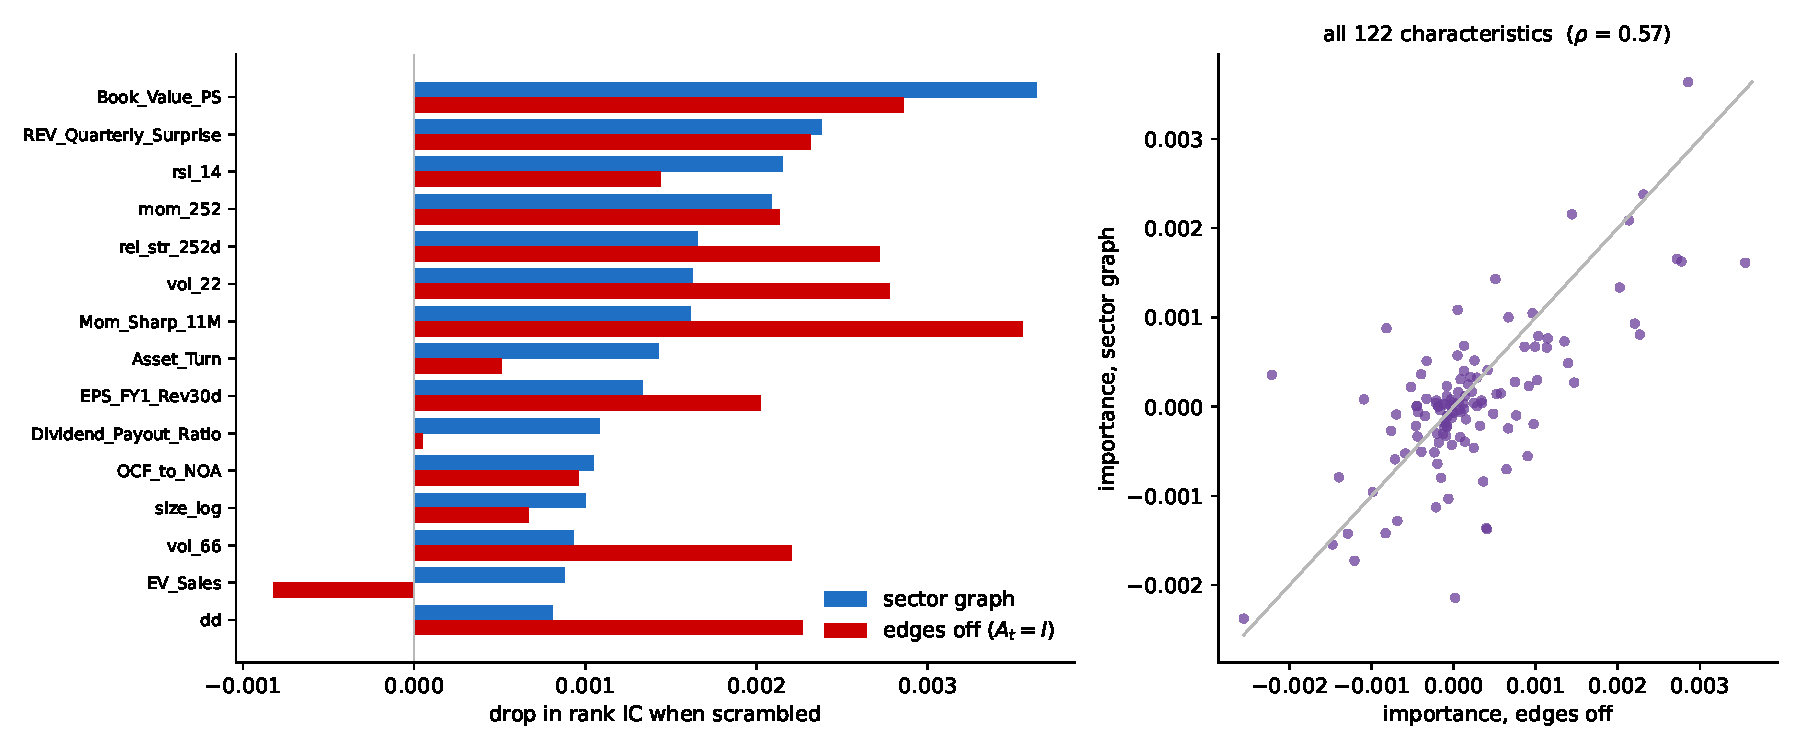
\includegraphics[width=0.7\linewidth]{files/figure_9_4_importanc-91b9b860bde5bf329c185f81ae3e8389.pdf}
\caption[]{Permutation importance of the 122 characteristics for the sector-graph GCN and its edge-free twin, on the fixed 2015 split. Left: the fifteen characteristics the graph model relies on most, measured by the drop in out-of-sample rank IC when each is scrambled within its date. Right: the importance of every characteristic under the graph against its importance without it, with Spearman correlation $\rho$.}
\label{fig-gnn-importance}
\end{figure}

\subsubsection{Coding exercises}\label{sec_gnn_exercises}

\begin{enumerate}
\item Compute the edge homophily ratio for a graph built from the finer NAICS subsector code rather than the sector code, and compare it with the sector value of 0.607. Does a narrower industry definition raise homophily, and does a GCN trained on it do any better against its edge-free twin?
\item Replace the sector graph by a correlation graph, connecting each firm to the ten others whose returns were most correlated over the preceding twelve months. Verify that the construction uses no information posterior to the formation date, and comment on the month-to-month turnover of the edge set.
\end{enumerate}

\subsubsection{References}

\subsection{Support vector machines}

While the origins of support vector machines (SVMs) are old (and go back to \cite{vapnik1963pattern}), their modern treatment was initiated in \cite{boser1992training} and \cite{cortes1995support} (binary classification) and \cite{drucker1997support} (regression). We refer to \href{http://www.kernel-machines.org/books}{http://www.kernel-machines.org/books} for an exhaustive bibliography on their theoretical and empirical properties. SVMs have been very popular since their creation among the machine learning community. Nonetheless, other tools (neural networks especially) have gained popularity and progressively replaced SVMs in many applications like computer vision notably.

\subsubsection{SVM for classification}

As is often the case in machine learning, it is easier to explain a complex tool through an illustration with binary classification. In fact, sometimes, it is originally how the tool was designed (e.g., for the perceptron). Let us consider a simple example in the plane, that is, with two features. In Figure~\ref{svmscheme}, the goal is to find a model that correctly classifies points: filled circles versus empty squares.

\begin{figure}[!htbp]
\centering
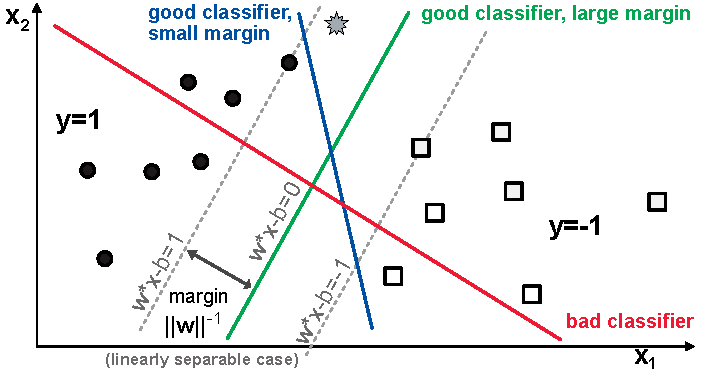
\includegraphics[width=0.625\linewidth]{files/svm-803b09e4fc2fd0cb8220fad1b82ec088.pdf}
\caption[]{Diagram of binary classification with support vectors.}
\label{svmscheme}
\end{figure}

A model consists of two weights $\textbf{w}=(w_1,w_2)$ that load on the variables and create a natural linear separation in the plane. In the example above, we show three separations. The red one is not a good classifier because there are circles and squares above and beneath it. The blue line is a good classifier: all circles are to its left and all squares to its right. Likewise, the green line achieves a perfect classification score. Yet, there is a notable difference between the two.

The grey star at the top of the graph is a mystery point and given its location, if the data pattern holds, it should be a circle. The blue model fails to recognize it as such while the green one succeeds. The interesting features of the scheme are those that we have not mentioned yet, that is, the grey dotted lines. These lines represent the no-man's land in which no observation falls when the green model is enforced. In this area, each strip above and below the green line can be viewed as a margin of error for the model. Typically, the grey star is located inside this margin.

The two margins are computed as the parallel lines that maximize the distance between the model and the closest points that are correctly classified (on both sides). These points are called \textbf{support vectors}, which justifies the name of the technique. Obviously, the green model has a greater margin than the blue one. The core idea of SVMs is to maximize the margin, under the constraint that the classifier does not make any mistake. Said differently, SVMs try to pick the most robust model among all those that yield a correct classification.

More formally, if we numerically define circles as +1 and squares as -1, any `good' linear model is expected to satisfy:

\begin{equation}
\label{eq:svm0}
\left\{\begin{array}{lll}
\sum_{k=1}^Kw_kx_{i,k}+b \ge +1 & \text{ when } y_i=+1 \\
\sum_{k=1}^Kw_kx_{i,k}+b \le -1 & \text{ when } y_i=-1,
\end{array}\right.
\end{equation}

which can be summarized in compact form $y_i \times \left(\sum_{k=1}^K w_kx_{i,k}+b \right)\ge 1$. Now, the margin between the green model and a support vector on the dashed grey line is equal to $||\textbf{w}||^{ -1}=\left(\sum_{k=1}^Kw_k^2\right)^{ -1/2}$. This value comes from the fact that the distance between a point $(x_0,y_0)$ and a line parametrized by $ax+by+c=0$ is equal to $d=\frac{|ax_0+by_0+c|}{\sqrt{a^2+b^2}}$. In the case of the model defined above \ref{eq:svm0}, the numerator is equal to 1 and the norm is that of $\textbf{w}$. Thus, the final problem is the following:

\begin{equation}
\label{eq:svm1}
\underset{\textbf{w}, b}{\text{argmin}} \ \frac{1}{2} ||\textbf{w}||^2 \ \text{ s.t. } y_i\left(\sum_{k=1}^Kw_kx_{i,k}+b \right)\ge 1.
\end{equation}

The dual form of this program (see chapter 5 in \cite{boyd2004convex}) is

\begin{equation}
\label{eq:svm1b}
L(\textbf{w},b,\boldsymbol{\lambda})=
 \frac{1}{2}||\textbf{w}||^2 + \sum_{i=1}^I\lambda_i\left(y_i\left(\sum_{k=1}^Kw_kx_{i,k}+b \right)- 1\right),
\end{equation}

where either $\lambda_i=0$ or $y_i\left(\sum_{k=1}^Kw_kx_{i,k}+b \right)= 1$. Thus, only some points will matter in the solution (the so-called support vectors). The first order conditions impose that the derivatives of this Lagrangian be null:

\begin{equation}
\frac{\partial L}{\partial \textbf{w}}L(\textbf{w},b,\boldsymbol{\lambda})=\textbf{0}, \quad \frac{\partial L}{\partial b}L(\textbf{w},b,\boldsymbol{\lambda})=0,
\end{equation}

where the first condition leads to

\begin{equation}
\textbf{w}^*=\sum_{i=1}^I\lambda_iu_i\textbf{x}_i.
\end{equation}

This solution is indeed a linear form of the features, but only some points are taken into account. They are those for which the inequalities \ref{eq:svm0} are equalities.

Naturally, this problem becomes infeasible whenever the condition cannot be satisfied, that is, when a simple line cannot perfectly separate the labels, no matter the choice of coefficients. This is the most common configuration and datasets are then called logically \textit{not linearly separable}. This complicates the process but it is possible to resort to a trick. The idea is to introduce some flexbility in \ref{eq:svm0} by adding correction variables that allow the conditions to be met:

\begin{equation}
\label{eq:svm2}
\left\{\begin{array}{lll}
\sum_{k=1}^Kw_kx_{i,k}+b \ge +1-\xi_i & \text{ when } y_i=+1 \\
\sum_{k=1}^Kw_kx_{i,k}+b \le -1+\xi_i & \text{ when } y_i=-1,
\end{array}\right.
\end{equation}

where the novelties, the $\xi_i$ are positive so-called \textbf{`slack' variables} that make the conditions feasible. They are illustrated in Figure~\ref{svmscheme2}. In this new configuration, there is no simple linear model that can perfectly discriminate between the two classes.

\begin{figure}[!htbp]
\centering
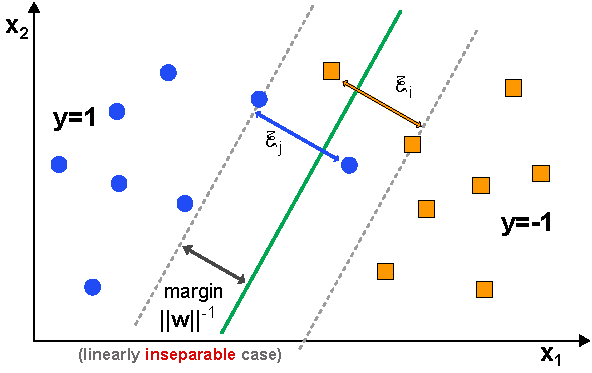
\includegraphics[width=0.625\linewidth]{files/svm2-f652c58a89424e044dacced0d8e3d5b6.pdf}
\caption[]{Diagram of binary classification with SVM - linearly inseparable data.}
\label{svmscheme2}
\end{figure}

The optimization program then becomes

\begin{equation}
\label{eq:svm3}
\underset{\textbf{w},b, \boldsymbol{\xi}}{\text{argmin}} \ \frac{1}{2} ||\textbf{w}||^2+C\sum_{i=1}^I\xi_i \ \text{ s.t. } \left\{ y_i\left(\sum_{k=1}^Kw_k\phi(x_{i,k})+b \right)\ge 1-\xi_i \ \text{ and } \ \xi_i\ge 0, \ \forall i  \right\},
\end{equation}

where the parameter $C>0$ tunes the cost of mis-classification: as $C$ increases, errors become more penalizing.

In addition, the program can be generalized to nonlinear models, via the kernel $\phi$ which is applied to the input points $x_{i,k}$. Nonlinear kernels can help cope with patterns that are more complex than straight lines (see Figure~\ref{svmscheme4}). Common kernels can be polynomial, radial or sigmoid. The solution is found using more or less standard techniques for constrained quadratic programs. Once the weights $\textbf{w}$ and bias $b$ are set via training, a prediction for a new vector $\textbf{x}_j$ is simply made by computing $\sum_{k=1}^Kw_k\phi(x_{j,k})+b$ and choosing the class based on the sign of the expression.

\begin{figure}[!htbp]
\centering
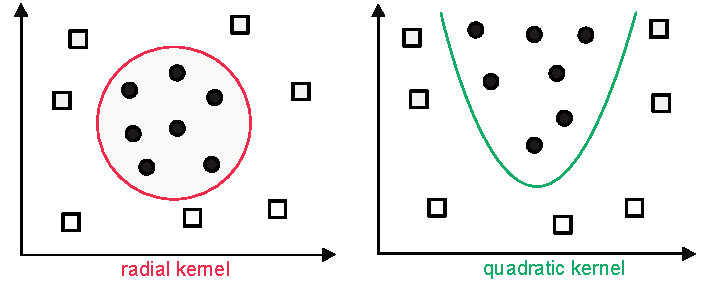
\includegraphics[width=0.5\linewidth]{files/kernel-c4ceac2655372255245b865b96528581.pdf}
\caption[]{Examples of nonlinear kernels.}
\label{svmscheme4}
\end{figure}

\subsubsection{SVM for regression}

The ideas of classification SVM can be transposed to regression exercises but the role of the margin is different. One general formulation is the following

\begin{equation}
\label{eq:svm4}
\begin{aligned}
\underset{\textbf{w},b, \boldsymbol{\xi}}{\text{argmin}} \  & \frac{1}{2} ||\textbf{w}||^2+C\sum_{i=1}^I\left(\xi_i+\xi_i^* \right)\\
 \text{ s.t. }&  \sum_{k=1}^Kw_k\phi(x_{i,k})+b -y_i\le \epsilon+\xi_i \\
&  y_i-\sum_{k=1}^Kw_k\phi(x_{i,k})-b \le \epsilon+\xi_i^* \\
&\xi_i,\xi_i^*\ge 0, \ \forall i  ,
\end{aligned}
\end{equation}

and it is illustrated in Figure~\ref{svmscheme3}. The user specifies a \textbf{margin} $\epsilon$ and the model will try to find the linear (up to kernel transformation) relationship between the labels $y_i$ and the input $\textbf{x}_i$. Just as in the classification task, if the data points are inside the strip, the slack variables $\xi_i$ and $\xi_i^*$ are set to zero. When the points violate the threshold, the objective function (first line of the code) is penalized. Note that setting a large $\epsilon$ leaves room for more error. Once the model has been trained, a prediction for $\textbf{x}_j$ is simply $\sum_{k=1}^Kw_k\phi(x_{j,k})+b$.

\begin{figure}[!htbp]
\centering
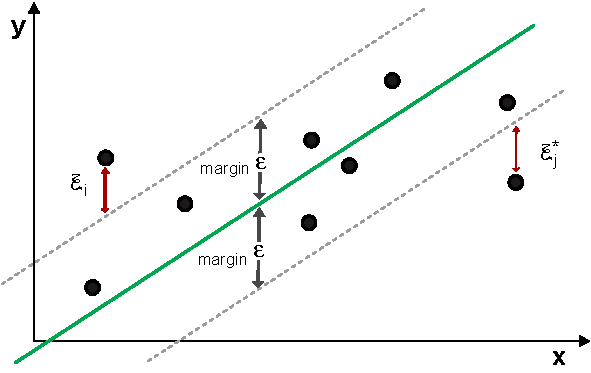
\includegraphics[width=0.625\linewidth]{files/svm3-f19cc71e59b778ccb6f885d525a469b0.pdf}
\caption[]{Diagram of regression SVM.}
\label{svmscheme3}
\end{figure}

Let us take a step back and simplify what the algorithm does, that is: minimize the sum of squared weights $||\textbf{w}||^2$ subject to the error being small enough (modulo a slack variable). In spirit, this somewhat the opposite of the penalized linear regressions which seek to minimize the error, subject to the weights being small enough.

The models laid out in this section are a preview of the universe of SVM engines and several other formulations have been developed. One reference library that is coded in C and C++ is \textbf{LIBSVM} and it is widely used by many other programming languages. The interested reader can have a look at the corresponding article \cite{chang2011libsvm} for more details on the SVM zoo (a more recent November 2019 version is also available online).

\subsubsection{Practice}

In Python, the LIBSVM library is exploited in scikit-learn through the \texttt{sklearn.svm} module. This provides both \texttt{SVR} (Support Vector Regression) and \texttt{SVC} (Support Vector Classification).

In the implementation of LIBSVM, the package requires to specify the label and features separately. For this reason, we recycle the variables used for the boosted trees. Moreover, the training being slow, we perform it on a subsample of these sets (first thousand instances).

\begin{verbatim}
from sklearn.svm import SVR
import numpy as np
import pandas as pd
import matplotlib.pyplot as plt
import seaborn as sns
import warnings
warnings.filterwarnings('ignore')
plt.style.use('seaborn-v0_8-whitegrid')
sns.set_palette("husl")

# Building the data & import functions
from data_build import generate_data
data_ml, features, features_short, returns, stock_ids, stock_ids_short = generate_data()
features_short =["Div_yld", "EPS", "size_avg_252d", "mom_252", "OCF_Growth_1Y", "PB", "vol_252"]
separation_date = "2017-01-15"

data_ml_clean = data_ml.dropna(subset=(features_short + ['R1M']))
training_sample = data_ml_clean[data_ml['date'] <= separation_date]
testing_sample = data_ml_clean[data_ml['date'] > separation_date]  #
\end{verbatim}

\begin{verbatim}
# Fit SVM for regression
fit_svm = SVR(
    kernel='rbf',        # SVM kernel (or: 'linear', 'poly', 'sigmoid')
    epsilon=0.1,         # Width of strip for errors
    gamma=0.5,           # Constant in the radial kernel
    C=0.1                # Slack variable penalisation
)

X_train = training_sample[features_short].iloc[0:1000]
y_train = training_sample['R1M'].iloc[0:1000]

# Train on first 1001 instances
fit_svm.fit(
    X_train,     # Training features
    y_train      # Training labels
)
\end{verbatim}

\begin{verbatim}
SVR(C=0.1, gamma=0.5)
\end{verbatim}

\begin{verbatim}
# Select test features
test_feat_short = testing_sample[features_short]

# Predictions
predictions = fit_svm.predict(test_feat_short)

# MSE
mse = np.mean((predictions - testing_sample['R1M'])**2)
print(f"MSE: {np.round(mse,5)}")

# Hit ratio
hit_ratio = np.mean(predictions * testing_sample['R1M'] > 0)
print(f"Hit ratio: {np.round(hit_ratio,5)}")
\end{verbatim}

\begin{verbatim}
MSE: 0.01591
Hit ratio: 0.52338
\end{verbatim}

The results are slightly better than those of the boosted trees. All parameters are completely arbitrary, especially the choice of the kernel. We finally turn to a classification example.

\begin{verbatim}
from sklearn.svm import SVC

# Fit SVM for classification
fit_svm_C = SVC(
    kernel='sigmoid',    # SVM kernel
    gamma=0.5,           # Parameter in the sigmoid kernel
    coef0=0.3,           # Parameter in the sigmoid kernel
    C=0.2                # Slack variable penalisation
)

# Train on first 1000 instances
fit_svm_C.fit(
    training_sample[features].iloc[:1000],     # Training features
    training_sample['R1M_C'].iloc[:1000]       # Training labels (classification)
)

# Accuracy
accuracy = np.mean(
    fit_svm_C.predict(testing_sample[features]) == testing_sample['R1M_C']
)
print(f"Accuracy: {np.round(accuracy,5)}")
\end{verbatim}

\begin{verbatim}
Accuracy: 0.49979
\end{verbatim}

Both the small training sample and the arbitrariness in our choice of the parameters may explain why the predictive accuracy is so poor.

\subsubsection{Coding exercises}

\begin{enumerate}
\item From the simple example shown above, extend SVM models to other kernels and discuss the impact on the fit.
\item Train a vanilla SVM model with labels being the 12-month forward (i.e., future) return and evaluate it on the testing sample. Do the same with a simple random forest. Compare.
\end{enumerate}

\subsection{Bayesian methods}

This section is dedicated to the subset of machine learning that makes prior assumptions on parameters. Before we explain how Bayes' theorem can be applied to simple building blocks in machine learning, we introduce some notations and concepts in the subsection below. Good references for Bayesian analysis are \cite{gelman2013bayesian} and \cite{kruschke2014doing}. The latter, like the present book, illustrates the concepts with many lines of R code. Bayesian inference is used in \cite{feng2021factor} to estimate conditional expected returns and residual covariance matrices with a view to portfolio choice.

\subsubsection{The Bayesian framework}

Up to now, the models that have been presented rely on data only. This approach is often referred to as `\textbf{frequentist}'. Given one dataset, a frequentist will extract (i.e., estimate) a unique set of optimal parameters and consider it to be the best model. Bayesians, on the other hand, consider datasets as \textbf{snapshots of reality} and, for them, parameters are thus random! Instead of estimating one value for parameters (e.g., a coefficient in a linear model), they are more ambitious and try to determine the \textbf{whole distribution} of the parameter.

In order to outline how that can be achieved, we introduce basic notations and results. The foundational concept in Bayesian analysis is the \textbf{conditional probability}. Given two random sets (or events) $A$ and $B$, we define the probability of $A$ knowing $B$ (equivalently, the odds of having $A$, conditionally on having $B$) as
\begin{equation}
P[A|B]=\frac{P[A \cap B]}{P[B]},
\end{equation}
that is, the probability of the intersection between the two sets divided by the probability of $B$. Likewise, the probability that both events occur is equal to $P[A \cap B] = P[A]P[B|A]$. Given $n$ disjoint events $A_i$, $i=1,...n$ such that $\sum_{i=1}^nP(A_i)=1$, then for any event $B$, the law of total probabilities is (or implies)
\begin{equation}
P(B)=\sum_{i=1}^nP(B \cap A_i)= \sum_{i=1}^nP(B|A_i)P(A_i).
\end{equation}

Given this expression, we can formulate a general version of Bayes' theorem:

\begin{equation}
\label{eq:bayes}
P(A_i|B)=\frac{P(A_i)P(B|A_i)}{P(B)}= \frac{P(A_i)P(B|A_i)}{\sum_{i=1}^nP(B|A_i)P(A_i)}.
\end{equation}

Endowed with this result, we can move forward to the core topic of this section, which is the estimation of some parameter $\boldsymbol{\theta}$ (possibly a vector) given a dataset, which we denote with $\textbf{y}$ thereby following the conventions from \cite{gelman2013bayesian}. This notation is suboptimal in this book nonetheless because in all other chapters, $\textbf{y}$ stands for the label of a dataset.

In Bayesian analysis, one sophistication (compared to a frequentist approach) comes from the fact that the data is not almighty. The distribution of the parameter $\boldsymbol{\theta}$ will be a mix between some \textbf{prior} distribution set by the statistician (the user, the analyst) and the empirical distribution from the data. More precisely, a simple application of Bayes' formula yields

\begin{equation}
\label{eq:bayes2}
p(\boldsymbol{\theta}| \textbf{y})=\frac{p(\boldsymbol{\theta})p(\textbf{y} |\boldsymbol{\theta})}{p(\textbf{y})} \propto p(\boldsymbol{\theta})p(\textbf{y} |\boldsymbol{\theta}).
\end{equation}

The interpretation is immediate: the distribution of $\boldsymbol{\theta}$ knowing the data $\textbf{y}$ is proportional to the distribution of $\boldsymbol{\theta}$ times the distribution of $\textbf{y}$ knowing $\boldsymbol{\theta}$. The term $p(\textbf{y})$ is often omitted because it is simply a scaling number that ensures that the density sums or integrates to one.

We use a slightly different notation between Equation \ref{eq:bayes} and Equation \ref{eq:bayes2}. In the former, $P$ denotes a true probability, i.e., it is a number. In the latter, $p$ stands for the whole probability density function of $\boldsymbol{\theta}$ or $\textbf{y}$.

The whole purpose of Bayesian analysis is to compute the so-called \textbf{posterior} distribution $p(\boldsymbol{\theta}| \textbf{y})$ via the \textbf{prior} distribution $p(\boldsymbol{\theta})$ and the \textbf{likelihood function} $p(\textbf{y} |\boldsymbol{\theta})$. Priors are sometimes qualified as informative, weakly informative or uninformative, depending on the degree to which the user is confident on the relevance and robustness of the prior. The simplest way to define a non-informative prior is to set a constant (uniform) distribution over some realistic interval(s).

The most challenging part is usually the likelihood function. The easiest way to solve the problem is to resort to a specific distribution (possibly a parametric family) for the distribution of the data and then consider that obsevations are i.i.d., just as in a simple maximum likelihood inference. If we assume that new parameters for the distributions are gathered into $\boldsymbol{\lambda}$, then the likelihood can be written as

\begin{equation}
\label{eq:likelihood}
p(\textbf{y} |\boldsymbol{\theta}, \boldsymbol{\lambda})=\prod_{i=1}^I f_{\boldsymbol{\lambda}}(y_i; \boldsymbol{\beta}),
\end{equation}

but in this case the problem becomes slightly more complex because adding new parameters changes the posterior distribution to $p(\boldsymbol{\theta}, \boldsymbol{\lambda}|\textbf{y})$. The user must find out the joint distribution of $\boldsymbol{\theta}$ and $\boldsymbol{\lambda}$ - given $\textbf{y}$. Because of their nested structure, these models are often called \textbf{hierarchical models}.

Bayesian methods are widely used for portfolio choice. The rationale is that the distribution of asset returns depends on some parameter and the main issue is to determine the posterior distribution. We very briefly review a vast literature below. Bayesian asset allocation is investigated in \cite{lai2011mean} (via stochastic optimization), \cite{guidolin2016ambiguity} and \cite{dangl2020optimal}. Shrinkage techniques (of means and covariance matrices) are tested in \cite{frost1986empirical}, \cite{kan2007optimal} and \cite{demiguel2015parameter}. In a similar vein, \cite{tu2010incorporating} build priors that are coherent with asset pricing theories. Finally, \cite{bauder2020bayesian} sample portfolio returns which allows to dervive a Bayesian optimal frontier. We invite the interested reader to also dwelve in the references that are cited within these few articles.

\subsubsection{Bayesian sampling}

\paragraph{Gibbs sampling}

One adjacent field of applications of Bayes' theorem is \textbf{simulation}. Suppose we want to simulate the multivariate distribution of a random vector $\textbf{X}$ given by its density $p=p(x_1,\dots,x_J)$. Often, the full distribution is complex, but its marginals are more accessible. Indeed, they are simpler because they depend on only one variable (when all other values are known):
\begin{equation}
p(X_j=x_j|X_1= x_1,\dots,X_{j-1}=x_{j-1},X_{j+1}=x_{j+1},\dots,X_J=x_J)=p(X_j=x_j|\textbf{X}_{-j}=\textbf{x}_{-j}),
\end{equation}
where we use the compact notation $\textbf{X}_{ -j}$ for all variables except $X_j$. One way to generate samples with law $p$ is the following and relies both on the knowledge of the conditionals $p(x_j|\textbf{x}_{ -j})$ and on the notion of \textbf{Markov Chain Monte Carlo}, which we outline below. The process is iterative and assumes that it is possible to draw samples of the aforementioned conditionals. We write $x_j^{m}$ for the $m^{th}$ sample of the $j^{th}$ variable ($X_j$). The simulation starts with a prior (or fixed, or random) sample $\textbf{x}^0=(x^0_1,\dots,x^0_J)$. Then, for a sufficiently large number of times, say $T$, new samples are drawn according to
\begin{align*}
x_1^{m+1} &= p(X_1|X_2=x_2^{m}, \dots ,X_J=x_J^m) ;\\
x_2^{m+1} &=p(X_2|X_1=x_1^{m+1}, X_3=x^{m}_3, \dots, X_J=x_J^m); \\
\dots& \\
x_J^{m+1}&= p(X_J|X_1=x_1^{m+1}, X_2=x_2^{m+1}, \dots, X_{J-1}=x_{J-1}^{m+1}).
\end{align*}

The important detail is that after each line, the value of the variable is updated. Hence, in the second line, $X_2$ is sampled with the knowledge of $X_1=x_1^{m+1}$ and in the last line, all variables except $X_J$ have been updated to their $(m+1)^{th}$ state. The above algorithm is called Gibbs sampling. It relates to Markov chains because each new iteration depends only on the previous one.

Under some technical assumptions, as $T$ increases, the distribution of $\textbf{x}_T$ converges to that of $p$. The conditions under which the convergence occurs have been widely discussed in series of articles in the 1990s. The interested reader can have a look for instance at \cite{tierney1994markov}, \cite{roberts1994simple}, as well as at section 11.7 of \cite{gelman2013bayesian}.

Sometimes, the full distribution is complex and the conditional laws are hard to determine and to sample. Then, a more general method, called Metropolis-Hastings, can be used that relies on the rejection method for the simulation of random variables.

\paragraph{Metropolis-Hastings sampling}

The Gibbs algorithm can be considered as a particular case of the Metropolis-Hastings (MH) method, which, in its simplest version, was introduced in \cite{metropolis1949monte}. The premise is similar: the aim is to simulate random variables that follow $p(\textbf{x})$ with the ability to sample from a simpler form $p(\textbf{x}|\textbf{y})$ which gives the probability of the future state $\textbf{x}$, given the past one $\textbf{y}$.

Once an initial value for $\textbf{x}$ has been sampled ($\textbf{x}_0$), each new iteration ($m$) of the simulation takes place in three stages:

\begin{enumerate}
\item generate a candidate value $\textbf{x}'_{m+1}$ from $p(\textbf{x}|\textbf{x}_m)$,
\item compute the acceptance ratio $\alpha=\min\left(\frac{p(\textbf{x}'_{m+1})p(\textbf{x}_{m}|\textbf{x}'_{m+1})}{p(\textbf{x}_{m})p(\textbf{x}'_{m+1}|\textbf{x}_{m})} \right)$
\item pick $\textbf{x}_{m+1}=\textbf{x}'_{m+1}$ with probability $\alpha$ or stick with the previous value ($\textbf{x}_{m+1}=\textbf{x}_{m}$) with probability $1 -\alpha$.
\end{enumerate}

The interpretation of the acceptance ratio is not straightforward in the general case. When the sampling generator is symmetric ($p(\textbf{x}|\textbf{y})=p(\textbf{y}|\textbf{x})$), the candidate is always chosen whenever $p(\textbf{x}'_{m+1})\ge p(\textbf{x}_{m})$. If the reverse condition holds ($p(\textbf{x}'_{m+1})< p(\textbf{x}_{m})$), then the candidate is retained with odds equal to $p(\textbf{x}'_{m+1})/p(\textbf{x}_{m})$, which is the ratio of likelihoods. The more likely the new proposal, the higher the odds of retaining it.

Often, the first simulations are discarded in order to leave time to the chain to converge to a high probability region. This procedure (often called `\textit{burn in}') ensures that the first retained samples are located in a zone that is likely, i.e., that they are more representative of the law we are trying to simulate.

For the sake of brevity, we stick to a succinct presentation here, but some additional details are outlined in section 11.2 of \cite{gelman2013bayesian} and in chapter 7 of \cite{kruschke2014doing}.

\subsubsection{Bayesian linear regression}

Because Bayesian concepts are rather abstract, it is useful to illustrate the theoretical notions with a simple example. In a linear model, $y_i=\textbf{x}_i\textbf{b}+\epsilon_i$ and it is often statistically assumed that the $\epsilon_i$ are i.i.d. and normally distributed with zero mean and variance $\sigma^2$. Hence, the likelihood of Equation \ref{eq:likelihood} translates into
\begin{equation}
p(\boldsymbol{\epsilon}|\textbf{b}, \sigma)=\prod_{i=1}^I\frac{e^{-\frac{\epsilon_i^2}{2\sigma}}}{\sigma\sqrt{2\pi}}=(\sigma\sqrt{2\pi})^{-I}e^{-\sum_{i=1}^I\frac{\epsilon_i^2}{2\sigma^2}}.
\end{equation}

In a regression analysis, the data is given both by $\textbf{y}$ and by $\textbf{X}$, hence both are reported in the notations. Simply acknowledging that $\boldsymbol{\epsilon}=\textbf{y} -\textbf{Xb}$, we get
\begin{align}
p(\textbf{y},\textbf{X}|\textbf{b}, \sigma)&=\prod_{i=1}^I\frac{e^{-\frac{\epsilon_i^2}{2\sigma}}}{\sigma\sqrt{2\pi}}\\
&=(\sigma\sqrt{2\pi})^{-I}e^{-\sum_{i=1}^I\frac{\left(y_i-\textbf{x}_i'\textbf{b}\right)^2}{2\sigma^2}}=(\sigma\sqrt{2\pi})^{-I} e^{-\frac{\left(\textbf{y}-\textbf{X}\textbf{b}\right)' \left(\textbf{y}-\textbf{X}\textbf{b}\right)}{2\sigma^2}} \\
&=\underbrace{(\sigma\sqrt{2\pi})^{-I} e^{-\frac{\left(\textbf{y}-\textbf{X}\hat{\textbf{b}}\right)' \left(\textbf{y}-\textbf{X}\hat{\textbf{b}}\right)}{2\sigma^2}}}_{\text{depends on } \sigma, \text{ not } \textbf{b}}\times \underbrace{e^{-\frac{(\textbf{b}-\hat{\textbf{b}})'\textbf{X}'\textbf{X}(\textbf{b}-\hat{\textbf{b}})}{2\sigma^2}}}_{\text{ depends on both } \sigma, \text{ and } \textbf{b} }.
\end{align}
In the last line, the second term is a function of the difference $\textbf{b} -\hat{\textbf{b}}$, where $\hat{\textbf{b}}=(\textbf{X}'\textbf{X})^{ -1}\textbf{X}'\textbf{y}$. This is not surprising: $\hat{\textbf{b}}$ is a natural benchmark for the mean of $\textbf{b}$. Moreover, introducing $\hat{\textbf{b}}$ yields a relatively simple form for the probability.

The above expression is the frequentist (data-based) block of the posterior: the likelihood. If we want to obtain a tractable expression for the posterior, we need to find a prior component that has a form that will combine well with this likelihood. These forms are called \textbf{conjugate priors}. A natural candidate for the right part (that depends on both \textbf{b} and $\sigma$) is the multivariate Gaussian density:

\begin{equation}
\label{eq:linprior}
p[\textbf{b}|\sigma]=\sigma^{-k}e^{-\frac{(\textbf{b}-\textbf{b}_0)'\boldsymbol{\Lambda}_0(\textbf{b}-\textbf{b}_0)}{2\sigma^2}},
\end{equation}

where we are obliged to condition with respect to $\sigma$. The density has prior mean $\textbf{b}_0$ and prior covariance matrix $\boldsymbol{\Lambda}_0^{ -1}$. This prior gets us one step closer to the posterior because
\begin{align}
p[\textbf{b},\sigma|\textbf{y},\textbf{X}]& \propto p[\textbf{y},\textbf{X}|\textbf{b},\sigma]p[\textbf{b},\sigma] \\
&\propto p[\textbf{y},\textbf{X}|\textbf{b},\sigma]p[\textbf{b}|\sigma]p[\sigma]. 
\end{align}

In order to fully specify the cascade of probabilities, we need to take care of $\sigma$ and set a density of the form

\begin{equation}
\label{eq:linsig}
p[\sigma^2]\propto (\sigma^2)^{-1-a_0}e^{-\frac{b_0}{2\sigma^2}},
\end{equation}

which is close to that of the left part of \ref{eq:linlike}. This corresponds to an inverse gamma distribution for the variance with prior parameters $a_0$ and $b_0$ (this scalar notation is not optimal because it can be confused with the prior mean $\textbf{b}_0$ so we must pay extra attention).

Now, we can simplify $p[\textbf{b},\sigma|\textbf{y},\textbf{X}]$ with \ref{eq:linlike}, \ref{eq:linprior} and \ref{eq:linsig}:
\begin{align*}
p[\textbf{b},\sigma|\textbf{y},\textbf{X}]& \propto 
(\sigma\sqrt{2\pi})^{-I} \sigma^{-2(1+a_0)} e^{-\frac{\left(\textbf{y}-\textbf{X}\hat{\textbf{b}}\right)' \left(\textbf{y}-\textbf{X}\hat{\textbf{b}}\right)}{2\sigma^2}} \\
&\quad \times e^{-\frac{(\textbf{b}-\hat{\textbf{b}})'\textbf{X}'\textbf{X}(\textbf{b}-\hat{\textbf{b}})}{2\sigma^2}}\sigma^{-k}e^{-\frac{(\textbf{b}-\textbf{b}_0)'\boldsymbol{\Lambda}_0(\textbf{b}-\textbf{b}_0)}{2\sigma^2}}e^{-\frac{b_0}{2\sigma^2}} \\
\end{align*}
which can be rewritten
\begin{align*}
p[\textbf{b},\sigma|\textbf{y},\textbf{X}]& \propto  \sigma^{-I-k-2(1+a_0)} \\
&\times  \exp\left(-\frac{\left(\textbf{y}-\textbf{X}\hat{\textbf{b}}\right)' \left(\textbf{y}-\textbf{X}\hat{\textbf{b}}\right) + (\textbf{b}-\hat{\textbf{b}})'\textbf{X}'\textbf{X}(\textbf{b}-\hat{\textbf{b}}) + (\textbf{b}-\textbf{b}_0)'\boldsymbol{\Lambda}_0(\textbf{b}-\textbf{b}_0)+b_0}{2\sigma^2} \right) .
\end{align*}

The above expression is simply a quadratic form in $\textbf{b}$ and it can be rewritten after burdensome algebra in a much more compact manner:

\begin{equation}
\label{eq:linpost}
p(\textbf{b}|\textbf{y},\textbf{X},\sigma) \propto \left[\sigma^{-k}e^{-\frac{(\textbf{b}-\textbf{b}_*)'\boldsymbol{\Lambda}_*(\textbf{b}-\textbf{b}_*)}{2\sigma^2}}\right] \times \left[ (\sigma^2)^{-1-a_*}e^{-\frac{b_*}{2\sigma^2}}  \right],
\end{equation}

where
\begin{align*}
\boldsymbol{\Lambda}_* &= \textbf{X}'\textbf{X}+\boldsymbol{\Lambda}_0  \\
\textbf{b}_*&=  \boldsymbol{\Lambda}_*^{-1}(\boldsymbol{\Lambda}_0\textbf{b}_0+\textbf{X}'\textbf{X}\hat{\textbf{b}}) \\
a_* & = a_0 + I/2  \\
b_* &=b_0+\frac{1}{2}\left(\textbf{y}'\textbf{y}+ \textbf{b}_0'\boldsymbol{\Lambda}_0\textbf{b}_0+\textbf{b}_*'\boldsymbol{\Lambda}_*\textbf{b}_* \right).\\
\end{align*}

This expression has two parts: the Gaussian component which relates mostly to $\textbf{b}$, and the inverse gamma component, entirely dedicated to $\sigma$. The mix between the prior and the data is clear. The posterior covariance matrix of the Gaussian part ($\boldsymbol{\Lambda}_*$) is the sum between the prior and a quadratic form from the data. The posterior mean $\textbf{b}_*$ is a weighted average of the prior $\textbf{b}_0$ and the sample estimator $\hat{\textbf{b}}$. Such blends of quantities estimated from data and a user-supplied version are often called \textbf{shrinkages}. For instance, the original matrix of cross-terms $\textbf{X}'\textbf{X}$ is shrunk towards the prior $\boldsymbol{\Lambda}_0$. This can be viewed as a \textbf{regularization} procedure: the pure fit originating from the data is mixed with some `external' ingredient to give some structure to the final estimation.

The interested reader can also have a look at section 16.3 of \cite{greene2018econometric} (the case of conjugate priors is treated in subsection 16.3.2).

The formulae above can be long and risky to implement. Luckily, there are Python packages that perform Bayesian inference for linear regression using conjugate priors. Below, we provide one example of how it works using PyMC. To simplify the code and curtail computation times, we consider two predictors: market capitalization (size anomaly) and price-to-book ratio (value anomaly). In statistics, the \textbf{precision matrix} is the inverse of the covariance matrix. In the parameters, the first two priors relate to the Gaussian law and the last two to the inverse gamma distribution:
\begin{equation}
f_\text{invgamma}(x, \alpha, \beta)=\frac{\beta^\alpha}{\Gamma(\alpha)}x^{-1-\alpha}e^{-\frac{\beta}{x}},
\end{equation}
where $\alpha$ is the shape and $\beta$ is the scale.

\begin{verbatim}
from sklearn.svm import SVR
import numpy as np
import pandas as pd
import matplotlib.pyplot as plt
import seaborn as sns
import warnings
warnings.filterwarnings('ignore')
plt.style.use('seaborn-v0_8-whitegrid')
sns.set_palette("husl")
import pymc as pm
import arviz as az

# Building the data & import functions
from data_build import generate_data
data_ml, features, features_short, returns, stock_ids, stock_ids_short = generate_data()
features_short =["Div_yld", "EPS", "size_avg_252d", "mom_252", "OCF_Growth_1Y", "PB", "vol_252"]
separation_date = "2017-01-15"

data_ml_clean = data_ml.dropna(subset=(features_short + ['R1M']))
training_sample = data_ml_clean[data_ml['date'] <= separation_date]
testing_sample = data_ml_clean[data_ml['date'] > separation_date]  #
\end{verbatim}

\begin{verbatim}
# Define prior parameters
prior_mean = np.array([0.01, 0.1, 0.1])  # Average value of parameters (prior)
prior_cov = np.diag(prior_mean**2)       # Covariance matrix of parameters (prior)

# Prepare data for Bayesian regression: size (Mkt_Cap_3M_Usd) and value (Pb)
X_train = testing_sample[['size_avg_252d', 'PB']].values
y_train = testing_sample['R1M'].values

# Build Bayesian linear model with PyMC
with pm.Model() as bayesian_lm:
    # Priors for regression coefficients (intercept + 2 predictors)
    beta = pm.MvNormal('beta', mu=prior_mean, cov=prior_cov, shape=3)
    
    # Prior for noise variance (inverse gamma)
    sigma = pm.InverseGamma('sigma', alpha=0.5, beta=0.5)
    
    # Expected value of outcome
    mu = beta[0] + beta[1] * X_train[:, 0] + beta[2] * X_train[:, 1]
    
    # Likelihood (sampling distribution) of observations
    y_obs = pm.Normal('y_obs', mu=mu, sigma=sigma, observed=y_train)
    
    # Sample from posterior
    trace = pm.sample(2000, return_inferencedata=True, progressbar=True)
\end{verbatim}

\begin{verbatim}
Initializing NUTS using jitter+adapt_diag...
\end{verbatim}

\begin{verbatim}
Multiprocess sampling (4 chains in 4 jobs)
\end{verbatim}

\begin{verbatim}
NUTS: [beta, sigma]
\end{verbatim}

\begin{verbatim}
Output()
\end{verbatim}

\begin{verbatim}
Sampling 4 chains for 1_000 tune and 2_000 draw iterations (4_000 + 8_000 draws total) took 43 seconds.
\end{verbatim}

In the above specification, we must also provide a prior for the constant. By default, we set its average value to 0.01, which corresponds to a 1\% average monthly return. Once the model has been estimated, we can plot the distribution of coefficient estimates.

\begin{verbatim}
# Extract posterior samples for beta coefficients
beta_samples = trace.posterior['beta'].values.reshape(-1, 3)

# Create DataFrame for plotting
beta_df = pd.DataFrame(beta_samples, columns=['Intercept', 'Size', 'Value'])
beta_melted = beta_df.melt(var_name='coefficient', value_name='value')

# Plot distribution of linear regression coefficients (betas)
fig, ax = plt.subplots(figsize=(8, 5))
for coef in ['Intercept', 'Size', 'Value']:
    data = beta_df[coef]
    ax.hist(data, bins=50, alpha=0.5, label=coef)
ax.set_xlabel('Value')
ax.set_ylabel('Count')
ax.legend(title='Coefficient')
ax.set_title('Distribution of linear regression coefficients (betas)')
plt.tight_layout()
plt.show()
\end{verbatim}

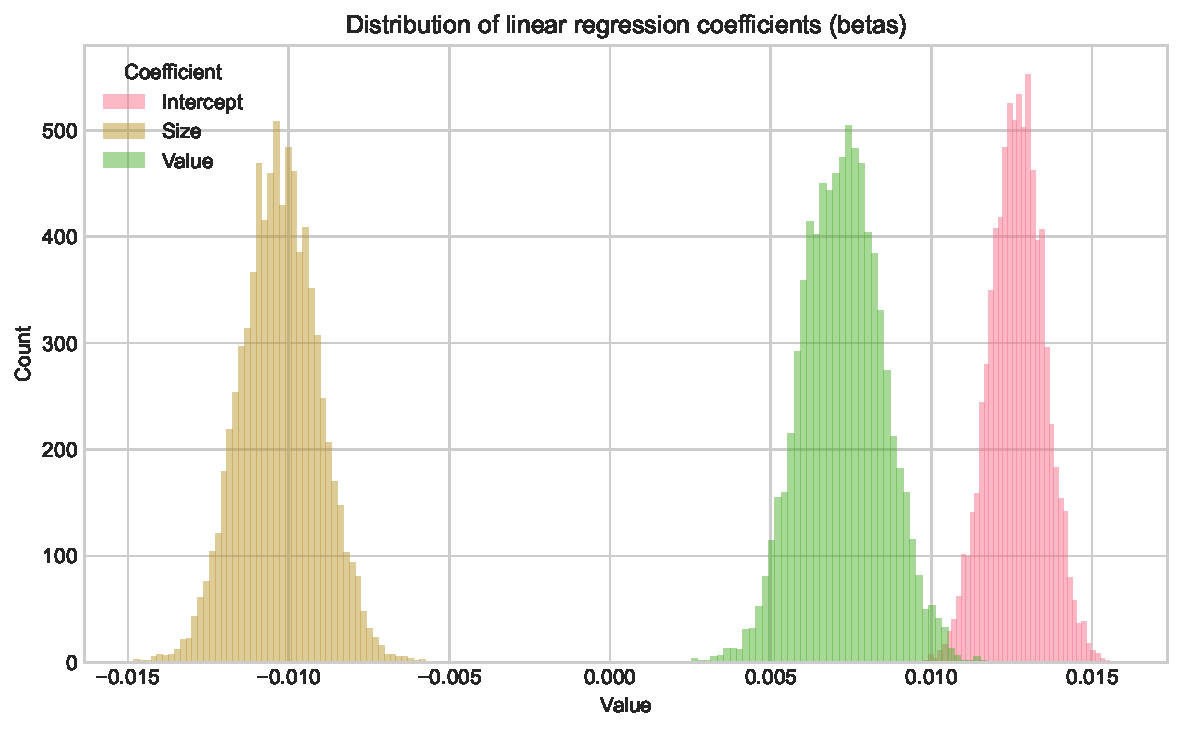
\includegraphics[width=0.7\linewidth]{files/f0ae124dfbc8c5e997ab2e92d5739686.pdf}

The distribution of the constant in the figure is firmly to the right with a small dispersion, hence it is solidly positive. For the size coefficient, it is the opposite; it is negative (small firms are more profitable). With regard to value, it is hard to conclude, the distribution is balanced around zero: there is no clear exposition to the price-to-book ratio variable.

\subsubsection{Naive Bayes classifier}

Bayes' theorem can also be easily applied to \textbf{classification}. We formulate it with respect to the label and features and write

\begin{equation}
\label{eq:naivebayes}
P[\textbf{y} | \textbf{X}] = \frac{P[ \textbf{X} | \textbf{y}]P[\textbf{y}]}{P[\textbf{X}]} \propto P[ \textbf{X} | \textbf{y}]P[\textbf{y}],
\end{equation}

and then split the input matrix into its column vectors $\textbf{X}=(\textbf{x}_1,\dots,\textbf{x}_K)$. This yields

\begin{equation}
\label{eq:naivebayes2}
P[\textbf{y} | \textbf{x}_1,\dots,\textbf{x}_K] \propto P[\textbf{x}_1,\dots,\textbf{x}_K| \textbf{y}]P[\textbf{y}].
\end{equation}

The `naive' qualification of the method comes from a simplifying assumption on the features.\footnote{This assumption can be relaxed, but the algorithms then become more complex and are out of the scope of the current book. One such example that generalizes the naive Bayes approach is \cite{friedman1997bayesian}.} If they are all mutually independent, then the likelihood in the above expression can be expanded into

\begin{equation}
\label{eq:naivebayes3}
P[\textbf{y} | \textbf{x}_1,\dots,\textbf{x}_K] \propto P[\textbf{y}]\prod_{k=1}^K P[\textbf{x}_k| \textbf{y}].
\end{equation}

The next step is to be more specific about the likelihood. This can be done non-parametrically (via kernel estimation) or with common distributions (Gaussian for continuous data, Bernoulli for binary data). In factor investing, the features are continuous, thus the Gaussian law is more adequate:
\begin{equation}
P[x_{i,k}=z|\textbf{y}_i= c]=\frac{e^{-\frac{(z-m_c)^2}{2\sigma_c^2}}}{\sigma_c\sqrt{2\pi}},
\end{equation}
where $c$ is the value of the classes taken by $y$ and $\sigma_c$ and $m_c$ are the standard error and mean of $x_{i,k}$, conditional on $y_i$ being equal to $c$. In practice, each class is spanned, the training set is filtered accordingly and $\sigma_c$ and $m_c$ are taken to be the sample statistics. This Gaussian parametrization is probably ill-suited to our dataset because the features are uniformly distributed. Even after conditioning, it is unlikely that the distribution will be even remotely close to Gaussian. Technically, this can be overcome via a double transformation method. Given a vector of features $\textbf{x}_k$ with empirical cdf $F_{\textbf{x}_k}$, the variable

\begin{equation}
\label{eq:transf}
\tilde{\textbf{x}}_k=\Phi^{-1}\left(F_{\textbf{x}_k}(\textbf{x}_k) \right),
\end{equation}

will have a standard normal law whenever $F_{\textbf{x}_k}$ is not pathological. Non-pathological cases are when the cdf is continuous and strictly increasing and when observations lie in the open interval (0,1). If all features are independent, the transformation should not have any impact on the correlation structure. Otherwise, we refer to the literature on the NORmal-To-Anything (NORTA) method (see, e.g., \cite{chen2001initialization} and \cite{coqueret2017approximate}).

Lastly, the prior $P[\textbf{y}]$ in Equation \ref{eq:naivebayes3} is often either taken to be uniform across the classes ($1/K$ for all $k$) or equal to the sample distribution.

We illustrate the naive Bayes classification tool with a simple example. While the scikit-learn library embeds such a classifier (GaussianNB), we show how to use it below. Since the features are uniformly distributed, the transformation in \ref{eq:transf} amounts to applying the Gaussian quantile function (inverse cdf).

For visual clarity, we only use the small set of features.

\begin{verbatim}
from sklearn.naive_bayes import GaussianNB

# Prepare training features (without transformation)
X_train_NB = training_sample[features_short].values
y_train_NB = training_sample['R1M_C'].values

# Fit basic Naive Bayes classifier
fit_NB_basic = GaussianNB()
fit_NB_basic.fit(X_train_NB, y_train_NB)

# Display model parameters
print(f"Naive Bayes model fitted with {len(features_short)} features")
print(f"Training samples: {len(training_sample)}")
print(f"Class prior probabilities: {fit_NB_basic.class_prior_}")
\end{verbatim}

\begin{verbatim}
Naive Bayes model fitted with 7 features
Training samples: 228548
Class prior probabilities: [0.50026253 0.49973747]
\end{verbatim}

\begin{verbatim}
from sklearn.naive_bayes import GaussianNB
from scipy.stats import norm

# Transform features using inverse Gaussian CDF (for uniformly distributed features)
def transform_features(data, features):
    """Apply Gaussian quantile transformation to features."""
    X = data[features].values
    X_clipped = np.clip(X, 0.0001, 0.9999)
    X_transformed = norm.ppf(X_clipped)
    return X_transformed

# Transform training features
gauss_features_train = transform_features(training_sample, features_short)

# Fit Naive Bayes classifier
fit_NB_gauss = GaussianNB()
fit_NB_gauss.fit(gauss_features_train, training_sample['R1M_C'])

print(f"Naive Bayes model fitted with {len(features_short)} features")
print(f"Training samples: {len(training_sample)}")
\end{verbatim}

\begin{verbatim}
Naive Bayes model fitted with 7 features
Training samples: 228548
\end{verbatim}

The plots show the distributions of the features, conditionally on each value of the label. Essentially, those are the densities $P[\textbf{x}_k| \textbf{y}]$. For each feature, both distributions are very similar.

As usual, once the model has been trained, the accuracy of predictions can be evaluated.

\begin{verbatim}
# Transform test features
gauss_features_test = transform_features(testing_sample, features_short)

# Compute hit ratio
predictions = fit_NB_gauss.predict(gauss_features_test)
hit_ratio = np.mean(predictions == testing_sample['R1M_C'])
print(f"Hit ratio: {hit_ratio:.4f}")
\end{verbatim}

\begin{verbatim}
Hit ratio: 0.5031
\end{verbatim}

The performance of the classifier is not satisfactory as it underperforms a random guess.

\subsubsection{Bayesian additive trees}\label{BART}

\paragraph{General formulation}

Bayesian additive regression trees (BARTs) are an ensemble technique that mixes Bayesian thinking and regression trees. In spirit, they are close to the tree ensembles seen in Chapter \href{/chap-07-trees}{Tree-based methods}, but they differ greatly in their implementation. In BARTs like in Bayesian regressions, the regularization comes from the prior. The original article is \cite{chipman2010bart} and the implementation (in R) follows \cite{sparapani2019r}. BARTs have been used in \cite{shu2021identifying} to identify which characteristics are priced. The authors report that stocks' market capitalization is the only one that matters.

Formally, the model is an aggregation of $M$ models, which we write as

\begin{equation}
\label{eq:BART}
y = \sum_{m=1}^M\mathcal{T}_m(q_m,\textbf{w}_m, \textbf{x}) + \epsilon,
\end{equation}

where $\epsilon$ is a Gaussian noise with variance $\sigma^2$, and the $\mathcal{T}_m=\mathcal{T}_m(q_m,\textbf{w}_m, \textbf{x})$ are decision trees with structure $q_m$ and weights vectors $\textbf{w}_m$. This decomposition of the tree is the one we used for boosted trees and is illustrated in the chapter on trees. $q_m$ codes all splits (variables chosen for the splits and levels of the splits) and the vectors $\textbf{w}_m$ correspond to the leaf values (at the terminal nodes).

At the macro-level, BARTs can be viewed as traditional Bayesian objects, where the parameters $\boldsymbol{\theta}$ are all of the unknowns coded through $q_m$, $\textbf{w}_m$ and $\sigma^2$ and where the focus is set on determining the posterior

\begin{equation}
\label{eq:bartpost}
\left(q_m,\textbf{w}_m,\sigma^2\right) | (\textbf{X}, \textbf{Y}).
\end{equation}

Given particular forms of priors for $\left(q_m,\textbf{w}_m,\sigma^2\right)$, the algorithm draws the parameters using a combination of Metropolis-Hastings \textit{and} Gibbs samplers.

\paragraph{Priors}

The definition of priors in tree models is delicate and intricate. The first important assumption is independence: independence between $\sigma^2$ and all other parameters and independence between trees, that is, between couples $(q_m,\textbf{w}_m)$ and $(q_n,\textbf{w}_n)$ for $m\neq n$. This assumption makes BARTs closer to random forests in spirit and further from boosted trees. This independence entails

\begin{equation}
P(\left(q_1,\textbf{w}_1\right),\dots,\left(q_M,\textbf{w}_M\right),\sigma^2)=P(\sigma^2)\prod_{m=1}^MP\left(q_m,\textbf{w}_m\right).
\end{equation}

Moreover, it is customary (for simplicity) to separate the structure of the tree ($q_m$) and the terminal weights ($\textbf{w}_m$), so that by a Bayesian conditioning

\begin{equation}
\label{eq:bart1}
P(\left(q_1,\textbf{w}_1\right),\dots,\left(q_M,\textbf{w}_M\right),\sigma^2)=\underbrace{P(\sigma^2)}_{\text{noise term}}\prod_{m=1}^M\underbrace{P\left(\textbf{w}_m|q_m\right)}_{\text{tree weights}}\underbrace{P(q_m)}_{\text{tree struct.}}
\end{equation}

It remains to formulate the assumptions for each of the three parts.

We start with the trees' structures, $q_m$. Trees are defined by their splits (at nodes) and these splits are characterized by the splitting variable and the splitting level. First, the size of trees is parametrized such that a node at depth $d$ is nonterminal with probability given by

\begin{equation}
\label{eq:bartnode}
\alpha(1+d)^{-\beta}, \quad \alpha \in (0,1), \quad \beta >0.
\end{equation}

The authors recommend to set $\alpha = 0.95$ and $\beta=2$. This gives a probability of 5\% to have 1 node, 55\% to have 2 nodes, 28\% to have 3 nodes, 9\% to have 4 nodes and 3\% to have 5 nodes. Thus, the aim is to force relatively shallow structures.

Second, the choice of splitting variables is driven by a generalized Bernoulli (categorical) distribution which defines the odds of picking one particular feature. In the original paper by \cite{chipman2010bart}, the vector of probabilities was uniform (each predictor has the same odds of being chosen for the split). This vector can also be random and sampled from a more flexible Dirichlet distribution. The level of the split is drawn uniformly on the set of possible values for the chosen predictor.

Having determined the prior of structure of the tree $q_m$, it remains to fix the terminal values at the leaves ($\textbf{w}_m|q_m$). The weights at all leaves are assumed to follow a Gaussian distribution $\mathcal{N}(\mu_\mu,\sigma_\mu^2)$, where $\mu_\mu=(y_\text{min}+y_\text{max})/2$ is the center of the range of the label values. The variance $\sigma_\mu^2$ is chosen such that $\mu_\mu$ plus or minus two times $\sigma_\mu^2$ covers 95\% of the range observed in the training dataset. Those are default values and can be altered by the user.

Lastly, for computational purposes similar to those of linear regressions, the parameter $\sigma^2$ (the variance of $\epsilon$ in \ref{eq:BART}) is assumed to follow an inverse Gamma law $\text{IG}(\nu/2,\lambda \nu/2)$ akin to that used in Bayesian regressions. The parameters are by default computed from the data so that the distribution of $\sigma^2$ is realistic and prevents overfitting. We refer to the original article, section 2.2.4, for more details on this topic.

In sum, in addition to $M$ (number of trees), the prior depends on a small number of parameters: $\alpha$ and $\beta$ (for the tree structure), $\mu_\mu$ and $\sigma_\mu^2$ (for the tree weights) and $\nu$ and $\lambda$ (for the noise term).

\paragraph{Sampling and predictions}

The posterior distribution in \ref{eq:bartpost} cannot be obtained analytically but simulations are an efficient shortcut to the model \ref{eq:BART}. Just as in Gibbs and Metropolis-Hastings sampling, the distribution of simulations is expected to converge to the sought posterior. After some burn-in sample, a prediction for a newly observed set $\textbf{x}_*$ will simply be the average (or median) of the predictions from the simulations. If we assume $S$ simulations after burn-in, then the average is equal to
\begin{equation}
\tilde{y}(\textbf{x}_*):=\frac{1}{S}\sum_{s=1}^S\sum_{m=1}^M\mathcal{T}_m\left(q_m^{(s)},\textbf{w}_m^{(s)}, \textbf{x}_*\right).
\end{equation}

The complex part is naturally to generate the simulations. Each tree is sampled using the Metropolis-Hastings method: a tree is proposed, but it replaces the existing one only under some (possibly random) criterion. This procedure is then repeated in a Gibbs-like fashion.

Let us start with the MH building block. We seek to simulate the conditional distribution

\begin{equation}
(q_m,\textbf{w}_m) \ | \ (q_{-m},\textbf{w}_{-m},\sigma^2, \textbf{y}, \textbf{x}),
\end{equation}

where $q_{ -m}$ and $\textbf{w}_{ -m}$ collect the structures and weights of all trees except for tree number $m$. One tour de force in BART is to simplify the above Gibbs draws to
\begin{equation}
(q_m,\textbf{w}_m) \ | \ (\textbf{R}_{m},\sigma^2 ),
\end{equation}
where $\textbf{R}_{m}=\textbf{y} -\sum_{l \neq m}\mathcal{T}_l(q_l,\textbf{w}_l, \textbf{x})$ is the partial residual on a prediction that excludes the $m^{th}$ tree.

The new MH proposition for $q_m$ is based on the previous tree and there are three possible (and random) alterations to the tree:

\begin{itemize}
\item growing a terminal node (increase the complexity of the tree by adding a supplementary leaf);
\item pruning a pair of terminal nodes (the opposite operation: reducing complexity);
\item changing splitting rules.
\end{itemize}

For simplicity, the third option is often excluded. Once the tree structure is defined (i.e., sampled), the terminal weights are independently drawn according to a Gaussian distribution $\mathcal{N}(\mu_\mu, \sigma_\mu^2)$.

After the tree is sampled, the MH principle requires that it be accepted or rejected based on some probability. This probability increases with the odds that the new tree increases the likelihood of the model. Its detailed computation is cumbersome and we refer to section 2.2 in \cite{sparapani2019r} for details on the matter.

Now, we must outline the overarching Gibbs procedure. First, the algorithm starts with trees that are simple nodes. Then, a specified number of loops include the following \textit{sequential} steps:

\bigskip\noindent
\begin{tabular}{p{\dimexpr 0.500\linewidth-2\tabcolsep}p{\dimexpr 0.500\linewidth-2\tabcolsep}}
\toprule
Step & Task \\
\hline
1 & sample \$(q\_1,{\textbackslash}textbf\{w\}\_1) {\textbackslash} \\
2 & sample \$(q\_2,{\textbackslash}textbf\{w\}\_2) {\textbackslash} \\
... & ...; \\
m & sample \$(q\_m,{\textbackslash}textbf\{w\}\_m) {\textbackslash} \\
... & ...; \\
M & sample \$(q\_M,{\textbackslash}textbf\{w\}\_M) {\textbackslash} \\
M+1 & sample $\sigma^2$ given the full residual $\textbf{R}=\textbf{y} -\sum_{l=1}^M\mathcal{T}_l(q_l,\textbf{w}_l, \textbf{x})$ \\
\bottomrule
\end{tabular}

\bigskip

At each step $m$, the residual $\textbf{R}_{m}$ is updated with the values from step $m -1$. We illustrate this process in the diagram below in which $M=3$. At step 1, a partition is proposed for the first tree, which is a simple node. In this particular case, the tree is accepted. In this scheme, the terminal weights are omitted for simplicity. At step 2, another partition is proposed for the tree, but it is rejected. In the third step, the proposition for the third is accepted. After the third step, a new value for $\sigma^2$ is drawn and a new round of Gibbs sampling can commence.

\begin{figure}[!htbp]
\centering
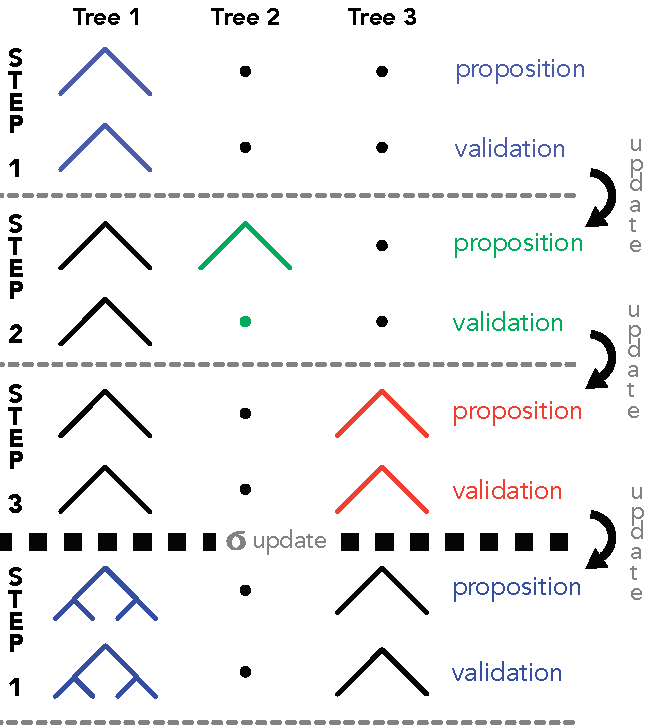
\includegraphics[width=0.325\linewidth]{files/bart-7ee850c94f98a8d8da5f039da14ac01e.pdf}
\caption*{Diagram of the MH/Gibbs sampling of BARTs. At step 2, the proposed tree is not validated.}
\end{figure}

\paragraph{Code}

There are several Python packages that implement BART methods. Below we use \texttt{pymc-bart} which integrates seamlessly with PyMC. We resort to only a few parameters, like \texttt{m} (number of trees $M$) and related hyperparameters. Nevertheless, the execution of the code takes time.

\begin{verbatim}
import pymc_bart as pmb

# Prepare data
X_train_bart = training_sample[features_short].values
y_train_bart = training_sample['R1M'].values
X_test_bart = testing_sample[features_short].values 

# Fit BART model using PyMC-BART
with pm.Model() as bart_model:
    X_shared = pm.Data('X', X_train_bart) 
    # BART prior for the mean function
    mu = pmb.BART('mu', X=X_shared, Y=y_train_bart, m=20)
    # Prior for noise
    sigma = pm.HalfNormal('sigma', sigma=1)  
    # Likelihood
    y_obs = pm.Normal('y_obs', mu=mu, sigma=sigma, observed=y_train_bart, shape=mu.shape)   
    # Sample from posterior
    idata = pm.sample(100, tune=20, progressbar=True, random_seed=42)
    # In-sample posterior predictive (training data)
    pp_train = pm.sample_posterior_predictive(idata, random_seed=42)
\end{verbatim}

\begin{verbatim}
Multiprocess sampling (4 chains in 4 jobs)
\end{verbatim}

\begin{verbatim}
CompoundStep
\end{verbatim}

\begin{verbatim}
>PGBART: [mu]
\end{verbatim}

\begin{verbatim}
>NUTS: [sigma]
\end{verbatim}

\begin{verbatim}
Output()
\end{verbatim}

\begin{verbatim}
Sampling 4 chains for 20 tune and 100 draw iterations (80 + 400 draws total) took 27 seconds.
\end{verbatim}

\begin{verbatim}
The rhat statistic is larger than 1.01 for some parameters. This indicates problems during sampling. See https://arxiv.org/abs/1903.08008 for details
\end{verbatim}

\begin{verbatim}
The effective sample size per chain is smaller than 100 for some parameters.  A higher number is needed for reliable rhat and ess computation. See https://arxiv.org/abs/1903.08008 for details
\end{verbatim}

\begin{verbatim}
Sampling: [y_obs]
\end{verbatim}

\begin{verbatim}
Output()
\end{verbatim}

Once the model is trained,\footnote{In the case of BARTs, the training consists exactly in the drawing of posterior samples.} we evaluate its performance. We simply compute the hit ratio.

\begin{verbatim}
with bart_model:                                                                                  
  pm.set_data({'X': X_test_bart})   
  pp_test = pm.sample_posterior_predictive(idata)
\end{verbatim}

\begin{verbatim}
Sampling: [mu, y_obs]
\end{verbatim}

\begin{verbatim}
Output()
\end{verbatim}

\begin{verbatim}
y_pred_bart = pp_test.posterior_predictive["y_obs"].values
y_pred_bart = y_pred_bart.mean(axis=(0, 1)) 
# Compute hit ratio (correct sign prediction)
hit_ratio_bart = np.mean(y_pred_bart * testing_sample['R1M'].values > 0)
print(f"Hit ratio: {hit_ratio_bart:.4f}")
\end{verbatim}

\begin{verbatim}
Hit ratio: 0.5284
\end{verbatim}

The performance \textit{seems} reasonable but is by no means impressive. The data from all sampled trees is available in the fitted model. The simplest information we can extract is the evolution of the model's residual standard deviation across iterations (approximating $\sigma$).

\begin{verbatim}
vi_results = pmb.compute_variable_importance(idata, mu, X_test_bart)
pmb.plot_variable_importance(vi_results)
\end{verbatim}

\begin{verbatim}
<Axes: ylabel='R²'>
\end{verbatim}

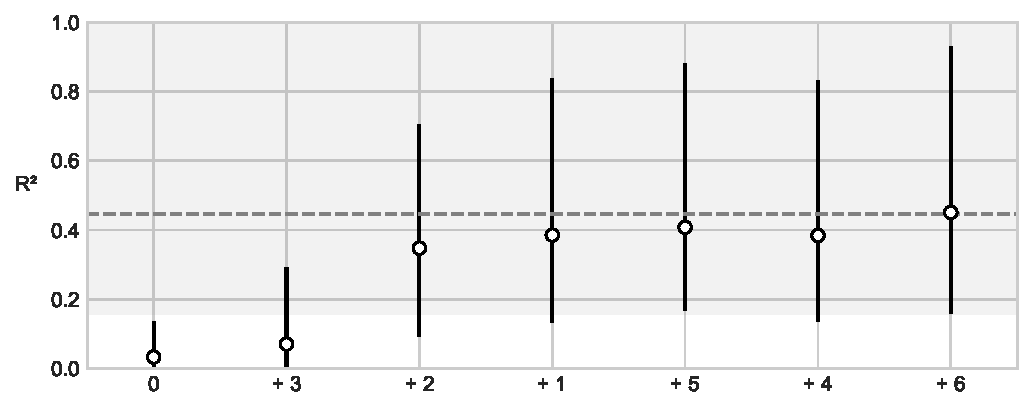
\includegraphics[width=0.7\linewidth]{files/55d1d55c5e052f9ff88e118a952e4b50.pdf}

\begin{verbatim}
from pymc_bart.utils import plot_pdp                                                              
                                                                                                    
fig, axes = plt.subplots(2, 4, figsize=(14, 7))                                                   
axes = axes.flatten()                                                                             
plot_pdp(bart_model['mu'], X=X_train_bart, Y=y_train_bart,                                        
           xs_interval='quantiles', grid=(2, 4), var_idx=list(range(len(features_short))),          
           var_discrete=None, func=None, samples=100, ax=axes[:len(features_short)])                
for i, feat in enumerate(features_short):                                                         
      axes[i].set_xlabel(feat)                                                                      
axes[-1].axis('off')  # Hide empty subplot                                                        
fig.suptitle('Partial Dependence Plots - BART Model', fontsize=14)                                
plt.tight_layout()                                                                                
plt.show()
\end{verbatim}

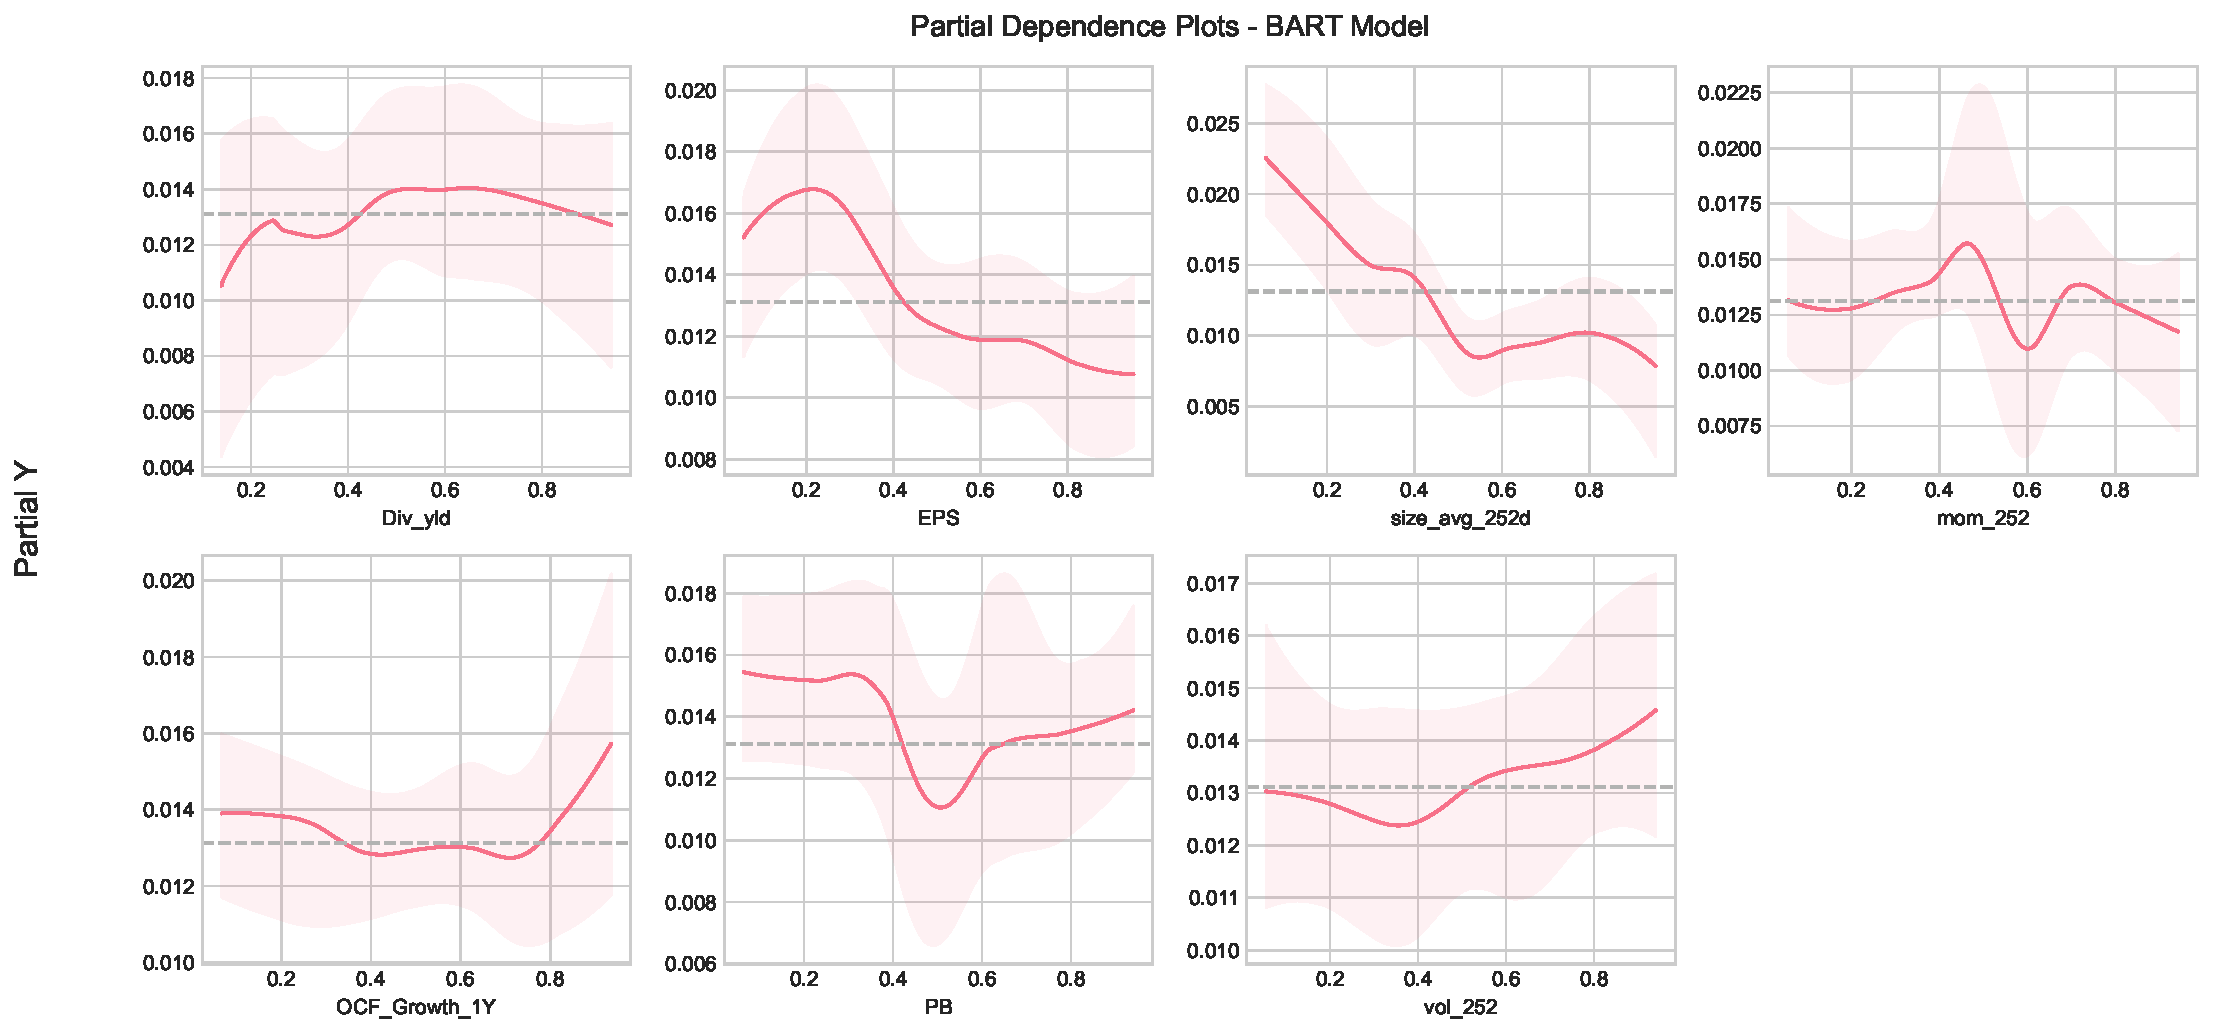
\includegraphics[width=0.7\linewidth]{files/fc66c759b30f5fb4b6a9eb3f9538afe3.pdf}

And we see that...

Individual Conditional Expectation (ICE) plots:

\begin{verbatim}
from pymc_bart.utils import plot_ice                                                              
                                                                                                    
fig, ax = plt.subplots(figsize=(8, 5))                                                            
plot_ice(bart_model['mu'], X=X_train_bart, Y=y_train_bart,                                        
           var_idx=[0], centered=True, samples=50, ax=ax)                                           
ax.set_xlabel(features_short[0])                                                                  
ax.set_title(f'ICE Plot for {features_short[0]}')                                                 
plt.tight_layout()                                                                                
plt.show()
\end{verbatim}

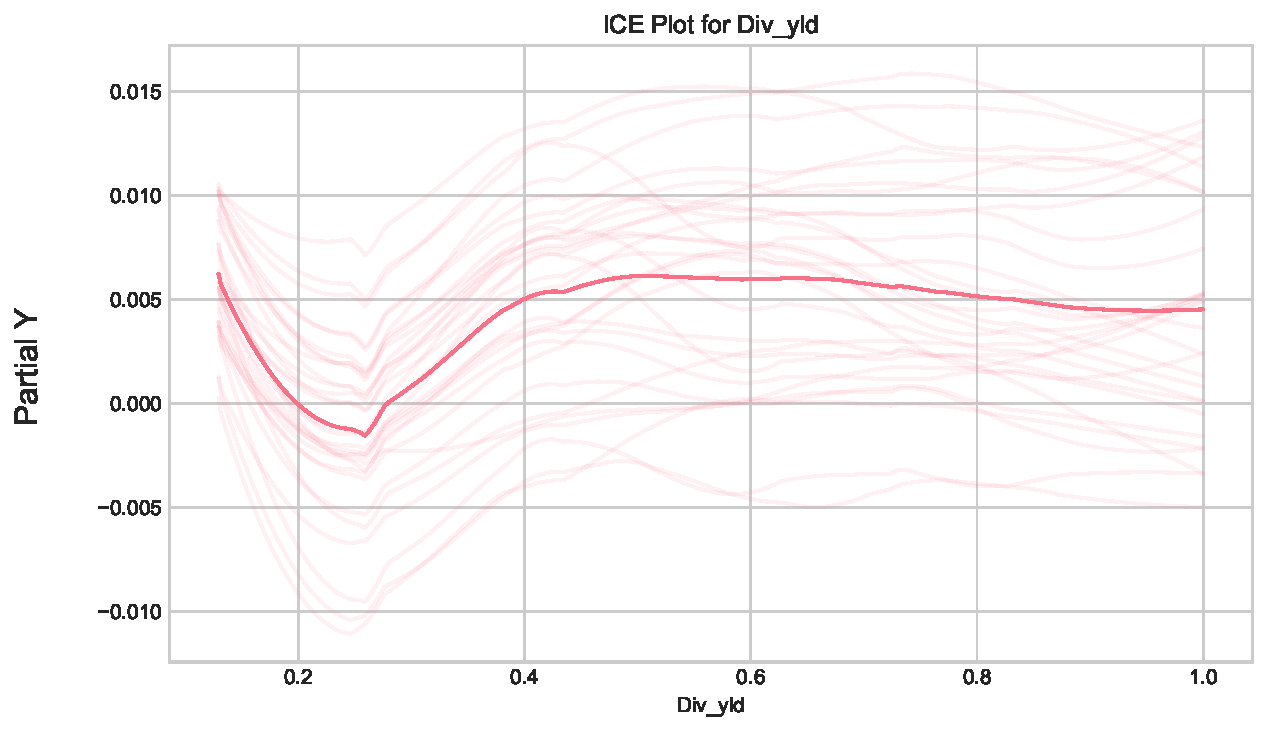
\includegraphics[width=0.7\linewidth]{files/44f7901a259b3eb7cb5c893fc0d4d155.pdf}

\subsection{Genetic algorithms for portfolio optimisation and factor investing}

% 
% Version: 0.5.6
% Last updated: 2026-07-29
% Versioning scheme:
%   MAJOR: structural overhaul, renumbering of top-level sections
%   MINOR: new section, new figure, new table, new content batch
%   PATCH: prose tweaks, citation additions, single-bib-entry fixes, typo fixes
% See `VERSIONING.md` in the chapter folder for the change log.
%

\subsubsection{Introduction}

\paragraph{Motivation}

Genetic algorithms conclude the sequence of supervised learning methods developed in this part of the book. The models of the preceding chapters, penalised regressions (Chapter 6), tree-based methods (Chapter 7), neural networks (Chapter 8), support vector machines (Chapter 9), and Bayesian methods (Chapter 10), share a common trait with the portfolio-construction, validation, and advanced-topic chapters that follow (Chapters 12 to 20): predictions and portfolio weights are obtained by solving some optimisation problem, whether it be a gradient descent over neural network weights, a quadratic program over portfolio allocations, or a Bayesian posterior computation.

In many practical settings, these optimisation problems are well-behaved. Gradient-based methods converge quickly when losses are smooth and convex, and quadratic programming solves the classical \cite{markowitz1952portfolio} mean-variance problem in polynomial time. Yet factor investing, by its very nature, involves selecting among a large number of candidate characteristics, the \cite{fama1993common} three-factor model has grown to hundreds of proposed anomalies \citep{harvey2016and}, and the constraints encountered in real-world implementations frequently shatter the convenient properties of standard optimisers:

\begin{itemize}
\item \textbf{Cardinality constraints.} A portfolio manager may be limited to holding at most $K$ out of $N$ assets. This transforms the continuous quadratic program into a mixed-integer problem that is NP-hard, as established by \cite{Bienstock1996} and \cite{Chang2000}.
\item \textbf{Discrete decisions.} Feature selection (Chapter 5, §5.4.1) involves binary include/exclude choices for each predictor. With $K$ candidate features, the search space has $2^K$ possible subsets, which for $K=122$ (the size of our dataset) is astronomically large.
\item \textbf{Non-convex objectives.} Maximising the Sharpe ratio, the Sortino ratio, or the Calmar ratio directly does not yield convex programs.
\item \textbf{Multiple competing objectives.} A systematic investor simultaneously seeks high returns, low variance, small drawdowns, limited turnover, and perhaps a favourable ESG score. These objectives conflict, and there is no single optimal solution, only a set of trade-offs among them.
\end{itemize}

Genetic algorithms (GAs) are a family of metaheuristic optimisation methods inspired by biological evolution \citep{Holland1975, Goldberg1989}. They maintain a \textit{population} of candidate solutions that evolve over successive \textit{generations} through \textit{selection}, \textit{crossover}, and \textit{mutation} operators, guided by a \textit{fitness function}. Because they do not require gradient information and can naturally handle discrete, combinatorial, and multi-objective problems, they are a natural complement to the gradient-based and Bayesian methods covered earlier in this book. In factor investing specifically, this makes them a natural tool for navigating the \textit{factor zoo}: the several hundred candidate anomalies now documented \citep{harvey2016and}, most of them mutually correlated or fragile out of sample, from which the investor must isolate a compact, robust subset. Much of this chapter can be read as a collection of evolutionary strategies for exactly that search.

In the context of factor investing, GAs have been applied to:

\begin{enumerate}
\item \textbf{Feature (factor) selection}: choosing which characteristics to include in a predictive model,
\item \textbf{Portfolio optimisation under complex constraints}: cardinality limits, round-lot requirements, sector caps,
\item \textbf{Hyperparameter tuning}: as an alternative to grid search (Chapter 12, §12.3.2) and Bayesian optimisation (§12.3.3),
\item \textbf{Alpha factor discovery}: using genetic programming (GP) to evolve mathematical expressions that predict returns,
\item \textbf{Multi-objective portfolio construction}: finding the Pareto front of return vs. risk vs. turnover.
\end{enumerate}

\paragraph{Historical evolution}

The academic literature on GAs in finance spans over three decades. We can identify five broad eras.

\textbf{Foundational period (1992 to 1999).} \cite{Bauer1992} were among the first to apply GAs to financial trading strategies. \cite{Arnone1993} extended GA optimisation to the Markowitz portfolio selection framework. The most influential work of this period is that of \cite{Allen1999}, published in the \textit{Journal of Financial Economics}. Using genetic programming to evolve technical trading rules for the S\&P 500 (1928 to 1995), they found that GP-evolved rules could identify periods of low volatility and high returns.

\textbf{Constraint integration era (2000 to 2010).} \cite{Chang2000} published the landmark study on cardinality-constrained portfolio optimisation, demonstrating that GAs, tabu search, and simulated annealing could solve problems that are intractable for exact solvers when the number of assets exceeds a few dozen. Their benchmark datasets are still used in comparative studies today. \cite{Maringer2003} extended this line of work with a hybrid local search algorithm that combined evolutionary search with exact local improvement steps. During this period, \cite{Deb2002} introduced the NSGA-II algorithm for multi-objective optimisation, which became the dominant method for Pareto-based portfolio construction.

\textbf{Factor-explicit era (2009 to 2019).} Research shifted from generic trading rules to explicit factor investing applications. \cite{Huang2012} demonstrated early success with a hybrid GA-SVM stock selection model, using GAs to select both features and SVM hyperparameters simultaneously. \cite{Kakushadze2016} published ``101 Formulaic Alphas.'' \cite{ZhangT2020} developed AutoAlpha, a hierarchical evolutionary algorithm for mining alpha factors with mutual information filtering to reduce redundancy. Concurrently, Bailey and López de Prado introduced the Deflated Sharpe Ratio, or DSR \citep{bailey2014deflated}, and \cite{bailey2017probability} the Probability of Backtest Overfitting (PBO) framework, providing essential tools for assessing whether GA-discovered strategies are genuine or artifacts of data mining.

\textbf{Deep learning integration era (2020 to 2023).} \cite{Liu2020} demonstrated that GP directly maximising the Sharpe ratio doubled performance compared to LASSO and neural network approaches in U.S. cross-sectional returns. Neuroevolution, evolving neural network architectures with methods such as NEAT \citep{Stanley2002} and EXAMM \citep{Lyu2024}, emerged as a way to automate the architectural choices discussed in Chapter 8. \cite{Yu2023} introduced AlphaGen, which uses proximal policy optimisation (PPO), a reinforcement learning method discussed in Chapter 20, to generate synergistic formulaic alpha collections, outperforming GP-based approaches in the KDD 2023 benchmark. \cite{Olorunda2024} provide a decade-spanning systematic survey confirming that GA-ML hybrids remain the dominant paradigm for stock market prediction.

\textbf{LLM-evolutionary era (2024 to present).} The most recent wave combines large language models with evolutionary search. Alpha-GPT \citep{wang2023alphagpt} pioneered human-AI interactive alpha mining via prompt engineering coupled with a GP-based search engine. Alpha-GPT 2.0 \citep{Yuan2024} extended this with specialised LLM agents for mining, modelling, and analysis. AlphaForge \citep{Shi2025} introduced a generative-predictive neural network that mines alpha factors and dynamically combines them with time-varying weights. AlphaAgent \citep{tang2025alphaagent} demonstrated autonomous alpha mining with regularised exploration, achieving 11\% annual excess return on the CSI 500, by incorporating AST-based originality enforcement and complexity control to counteract alpha decay. \cite{Han2026} pushed the frontier further with QuantaAlpha by treating each mining run as a trajectory and applying trajectory-level mutation and crossover operations, achieving an IC of 0.15 with strong cross-market transfer. \cite{ZhangJ2025} provide the first comprehensive survey of LLM-based alpha mining from an agentic perspective, identifying key challenges including limited numerical understanding, lack of diversity, weak exploration dynamics, and temporal data leakage. This rapid evolution (from hand-crafted rules in the 1990s, to population-based search in the 2000s, to neural architecture evolution in the 2020s, to LLM-guided discovery from 2024 onwards) underscores both the vitality of evolutionary methods in finance and the importance of rigorous validation (§11.7.1) as the pace of discovery accelerates.

\subsubsection{Genetic algorithm fundamentals}

\paragraph{What is a genetic algorithm?}

A genetic algorithm is a population-based metaheuristic that solves optimisation problems by mimicking the process of natural selection. The key metaphor maps directly from biology to optimisation:

\bigskip\noindent
\begin{tabular}{p{\dimexpr 0.500\linewidth-2\tabcolsep}p{\dimexpr 0.500\linewidth-2\tabcolsep}}
\toprule
Biology & Optimisation \\
\hline
Individual organism & Candidate solution \\
Chromosome (genotype) & Encoded representation of a solution \\
Gene & Single element of the encoding \\
Phenotype & Decoded solution \\
Fitness & Objective function value \\
Population & Set of candidate solutions \\
Generation & One iteration of the algorithm \\
Selection & Retaining high-quality solutions \\
Crossover (recombination) & Combining parts of two solutions \\
Mutation & Random perturbation of a solution \\
\bottomrule
\end{tabular}

\bigskip

We summarise this mapping in TABLE 11.1.

TABLE 11.1: Mapping between biological evolution and GA optimisation.

The core idea is simple: start with a random population of candidate solutions, evaluate how good each one is (fitness), select the better ones to reproduce, combine them (crossover) and introduce small random changes (mutation), and repeat. Over generations, the population evolves toward better solutions.

Formally, let $\mathbf{x} \in \mathcal{X}$ be a candidate solution in some search space $\mathcal{X}$, and let $f: \mathcal{X} \rightarrow \mathbb{R}$ be the fitness function to maximise. A GA operates on a population $P^{(g)} = \{\mathbf{x}_1^{(g)}, \ldots, \mathbf{x}_N^{(g)}\}$ at generation $g$ and produces $P^{(g+1)}$ through the application of selection, crossover, and mutation operators.

\cite{Holland1975} provided the first theoretical justification for GAs through the \textit{Schema Theorem}. A \textbf{schema} is a template that matches a subset of chromosomes: for example, the schema \texttt{1**0*1} matches all binary strings with a 1 in positions 1 and 6, a 0 in position 4, and any value elsewhere (where \texttt{*} is a wildcard). The theorem states that short, low-order schemata with above-average fitness receive exponentially increasing representation in successive generations. Informally, GAs implicitly evaluate a large number of short `building blocks' in parallel and combine the best ones. \cite{Goldberg1989} formalised this intuition as the \textbf{Building Block Hypothesis}: GAs work well when short, fit schemata can be recombined to form even fitter solutions.

The Building Block Hypothesis is an idealisation. In practice, \textit{epistasis} (interactions between genes) and \textit{deception} (where locally fit building blocks mislead the search toward suboptimal regions) can undermine it. For the financial applications in this chapter, the practical implication is that GAs work best when the fitness contribution of each gene (e.g., whether to include a particular factor) is relatively independent, making the building blocks short and combinable. When strong interactions exist between features, the GA may require larger populations and more generations to discover fit combinations.

\paragraph{How GAs differ from other optimisers}

It is useful to position GAs relative to the optimisation methods encountered in earlier chapters. TABLE 11.2 provides a concise comparison.

\bigskip\noindent
\begin{tabular}{p{\dimexpr 0.200\linewidth-2\tabcolsep}p{\dimexpr 0.200\linewidth-2\tabcolsep}p{\dimexpr 0.200\linewidth-2\tabcolsep}p{\dimexpr 0.200\linewidth-2\tabcolsep}p{\dimexpr 0.200\linewidth-2\tabcolsep}}
\toprule
Property & Gradient descent (Ch. 7) & Bayesian opt. (§12.3.3) & Grid/random search (§12.3.2) & Genetic algorithm \\
\hline
Requires gradient? & Yes & No & No & No \\
Handles discrete variables? & No & With difficulty & Yes & Yes \\
Handles constraints? & Via Lagrangians & Via penalties & Natively & Natively \\
Multi-objective? & Scalarisation needed & Single objective & No & Yes (NSGA-II) \\
Parallelisable? & Limited & Sequential (acquisition) & Fully & Fully \\
Risk of local optima? & High & Low (with GP prior) & None (exhaustive) & Low (population diversity) \\
Computational cost & Low per iteration & High (surrogate model) & Explodes with dimension & Moderate (population $\times$ generations) \\
\bottomrule
\end{tabular}

\bigskip

TABLE 11.2: Comparison of optimisation methods.

GAs are particularly attractive when: (i) the search space is discrete or mixed, (ii) the objective function is non-differentiable or noisy, (iii) constraints are complex and heterogeneous, and (iv) the user wants a set of diverse solutions rather than a single optimum.

\paragraph{The GA workflow}

The generic GA proceeds as follows:

\textbf{Algorithm 11.1: Generic Genetic Algorithm}

\begin{verbatim}
Input: fitness function f, population size N, number of generations G,
       crossover probability p_c, mutation probability p_m
Output: best solution found

1. Initialise: generate P^(0) = {x_1, ..., x_N} randomly
2. For g = 0, 1, ..., G -1:
   a. Evaluate: compute f(x_i) for all x_i in P^(g)
   b. Select: choose N parents from P^(g) based on fitness
   c. Crossover: for each pair of parents, with probability p_c,
      recombine to produce offspring
   d. Mutate: for each offspring, with probability p_m, apply
      random perturbation
   e. Replace: form P^(g+1) from offspring (possibly retaining
      elite individuals)
3. Return: argmax_{x in P^(G)} f(x)
\end{verbatim}

In practice, an \textit{elitism} mechanism ensures that the best individual from generation $g$ is always carried over to generation $g+1$, preventing the loss of the best-known solution.

\paragraph{Genetic algorithms versus genetic programming}

A distinction that is important for financial applications is the one between GAs and genetic programming (GP). In a standard GA, the chromosome has a \textbf{fixed length} (for instance, a binary vector of length $K$ for feature selection, or a real vector of length $N$ for portfolio weights). In GP, the chromosome is a \textbf{variable-length tree} representing a mathematical expression. The leaves (terminals) are variables or constants, and the internal nodes are operators ($+, -, \times, \div, \log, \text{abs}, \ldots$).

This distinction matters because GP can discover \textbf{new factors} by composing elementary data fields, whereas a standard GA can only select or weight factors from a predefined universe. For example, GP might evolve the expression $\text{rank}(\text{close}/\text{delay}(\text{close}, 5)) - \text{rank}(\text{volume}/\text{adv20})$, which is a formulaic alpha of the type catalogued by \cite{Kakushadze2016}. We explore this application in §11.4.4.

Because the GP implementation in §11.4.4 relies on several concepts that differ substantially from standard GAs, we provide additional detail here. A GP tree has \textbf{internal nodes} drawn from a set of operators (the \textit{function set}, e.g., $+, -, \times$, protected division) and \textbf{leaf nodes} drawn from a set of terminals (input variables such as \texttt{close}, \texttt{volume}, and random constants). Together, these form the \textbf{primitive set} that defines the space of expressible programs. For instance, the expression $(x_1 \times x_1) + 2.0$ corresponds to a tree with $+$ at the root, a $\times$ subtree on the left (with $x_1$ as both leaves), and the constant 2.0 on the right.

A key requirement is the \textbf{closure property}: every operator must accept as input any value that another operator or terminal can produce. Division is problematic because it is undefined at zero. The standard remedy is \textit{protected division}, defined as $\text{div}(a, b) = a/b$ if $|b| > \epsilon$ and 0 otherwise, where $\epsilon$ is a small tolerance. Without this safeguard, randomly generated trees frequently produce runtime errors.

Initial trees are created via a procedure known as \textit{ramped half-and-half} \citep{Koza1992}: half the population is built as full trees (every branch extends to the maximum depth) and half as grow trees (branches terminate at random depths), with the depth limit varied across the population. This ensures a diverse mix of tree sizes. Over successive generations, trees tend to grow larger without corresponding fitness improvements, a phenomenon called \textbf{bloat}. Standard countermeasures include static depth limits (e.g., a maximum depth of 8) and parsimony pressure, which adds a penalty proportional to tree size to the fitness function.

The genetic operators in GP also differ from their GA counterparts (contrast with §11.3.4 and §11.3.5). \textbf{Tree crossover} swaps randomly selected subtrees between two parent trees, which is fundamentally different from the segment-swapping crossover used for fixed-length binary strings. \textbf{Subtree mutation} replaces a random subtree with a newly generated one. Both operators preserve tree validity because the primitive set enforces closure at every node. We implement these concepts in §11.4.4 using DEAP's \texttt{gp} module, which provides tree generation (\texttt{genHalfAndHalf}), compilation of trees to callable Python functions (\texttt{gp.compile}), and bloat control via \texttt{gp.staticLimit}.

\paragraph{Toy example: a miniature feature-selection GA}

Before turning to the full financial applications, let us implement a GA from scratch on the simplest possible financial problem. From a small pool of $L = 14$ candidate features, we search for the binary subset whose equal-weighted composite best predicts next-month returns. Each chromosome is a binary mask (gene $k$ is 1 when feature $k$ is included), and the fitness is the cross-sectional Information Coefficient (IC) of the resulting composite. This is the financial analogue of the classic OneMax benchmark (find the binary string maximising the number of 1s): where OneMax counts the 1s, here we measure predictive power. Crucially, the optimum is no longer the all-ones vector, because redundant or noisy features dilute the composite.

This example illustrates every GA component in a handful of lines, with no external optimisation library: initialisation, fitness evaluation, tournament selection, single-point crossover, bit-flip mutation, and elitism. We begin by assembling the feature pool and the fitness function.

\begin{verbatim}
import numpy as np
import pandas as pd
import random
from scipy.stats import spearmanr
import matplotlib.pyplot as plt

# -- Reproducibility ------------------------------------------
SEED = 42
np.random.seed(SEED)
random.seed(SEED)

# -- A small pool of 14 candidate features ---------------------
data_ml = pd.read_parquet('data/mlfi_us_data.parquet')
data_ml = data_ml.rename(columns={'id': 'stock_id'})
pool = ['mom_252', 'vol_252', 'size_log', 'PB', 'ROE', 'Div_yld',
        'rel_str_252d', 'idio_vol_252d', 'Asset_Turn', 'Current_Ratio',
        'Interest_Coverage', 'kurt_252', 'bb_width', 'Cash_to_Assets']
L = len(pool)            # 14 candidate features

# Cross-sectional z-score each feature, then take an in-sample slice
df = data_ml[data_ml['date'].between('2015-01-01', '2019-12-31')]
df = df.dropna(subset=pool + ['R1M_Usd']).copy()
for f in pool:
    g = df.groupby('date')[f]
    df[f] = ((df[f] - g.transform('mean')) / g.transform('std')).clip(-5, 5).fillna(0)
df = df.sample(n=20000, random_state=SEED)
y = df['R1M_Usd'].values

# Sign each feature by its own IC so the composite does not self-cancel
signs = np.array([np.sign(spearmanr(df[f].values, y)[0]) for f in pool])
signed_z = df[pool].values * signs

def fitness(mask):
    """Cross-sectional IC of the equal-weighted composite of selected features."""
    m = np.asarray(mask, dtype=bool)
    if m.sum() == 0:
        return 0.0
    return spearmanr(signed_z[:, m].mean(axis=1), y)[0]
\end{verbatim}

The genetic operators and the evolution loop are written out in full; this is the same scaffolding that every application later in the chapter delegates to a library.

\begin{verbatim}
# -- GA parameters --------------------------------------------
POP_SIZE = 20            # Population size
N_GEN = 30               # Number of generations
P_CROSS = 0.9            # Crossover probability
P_MUT = 1.0 / L          # Per-gene mutation probability
TOURN_K = 3              # Tournament size

# -- Initialise population (random binary masks) --------------
pop = [np.random.randint(0, 2, size=L) for _ in range(POP_SIZE)]

# -- Tournament selection -------------------------------------
def tournament(pop, scores, k=TOURN_K):
    idx = random.sample(range(len(pop)), k)
    best = max(idx, key=lambda i: scores[i])
    return pop[best].copy()

# -- Single -point crossover -----------------------------------
def crossover(p1, p2):
    if random.random() < P_CROSS:
        pt = random.randint(1, L - 1)    # Crossover point
        c1 = np.concatenate([p1[:pt], p2[pt:]])
        c2 = np.concatenate([p2[:pt], p1[pt:]])
        return c1, c2
    return p1.copy(), p2.copy()

# -- Bit -flip mutation ----------------------------------------
def mutate(x):
    for i in range(L):
        if random.random() < P_MUT:
            x[i] = 1 - x[i]              # Flip bit
    return x

# -- Evolution loop -------------------------------------------
best_hist, avg_hist = [], []
for g in range(N_GEN):
    scores = np.array([fitness(x) for x in pop])
    best_hist.append(scores.max())
    avg_hist.append(scores.mean())

    # Elitism: carry over the best individual
    elite = pop[int(np.argmax(scores))].copy()

    # Create next generation
    children = [elite]                    # Elitism slot
    while len(children) < POP_SIZE:
        p1 = tournament(pop, scores)
        p2 = tournament(pop, scores)
        c1, c2 = crossover(p1, p2)
        children.append(mutate(c1))
        if len(children) < POP_SIZE:
            children.append(mutate(c2))
    pop = children

# -- Results --------------------------------------------------
final = np.array([fitness(x) for x in pop])
best = pop[int(np.argmax(final))]
selected = [pool[i] for i in range(L) if best[i]]
print(f"Best composite IC: {final.max():.4f}")
print(f"Selected {int(best.sum())} / {L}: {selected}")
print(f"IC of all-{L}-feature composite: {fitness(np.ones(L)):.4f}")
\end{verbatim}

\begin{verbatim}
Best composite IC: 0.0466
Selected 8 / 14: ['vol_252', 'size_log', 'PB', 'Div_yld',
  'idio_vol_252d', 'Current_Ratio', 'Interest_Coverage', 'bb_width']
IC of all-14-feature composite: 0.0412
\end{verbatim}

\begin{verbatim}
# -- Convergence plot -----------------------------------------
fig, ax = plt.subplots(figsize=(8, 4))
ax.plot(best_hist, label="Best IC", linewidth=2)
ax.plot(avg_hist, label="Average IC", linewidth=1,
        linestyle="--")
ax.set_xlabel("Generation")
ax.set_ylabel("Composite IC")
ax.set_title("Miniature feature-selection GA: convergence")
ax.legend()
plt.tight_layout()
plt.show()
\end{verbatim}

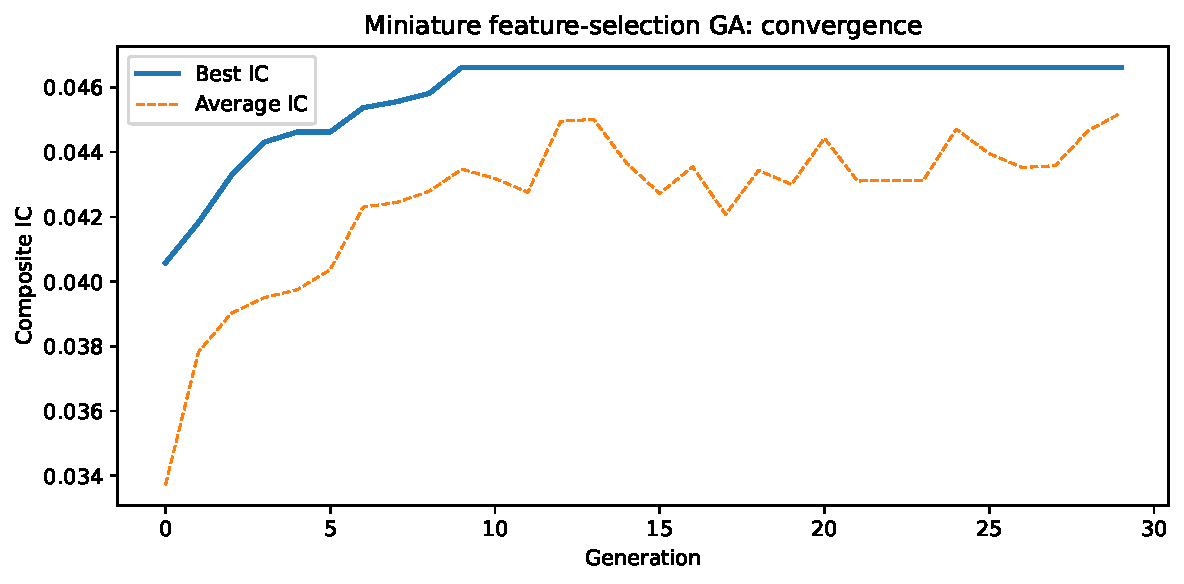
\includegraphics[width=0.7\linewidth]{files/7b3c8b0bc8ad6f8ca511168788502f59.pdf}

FIGURE 11.1: Convergence of the miniature feature-selection GA. The best composite IC climbs from about 0.041 to 0.047 within roughly nine generations and then plateaus, while the average population IC rises more gradually and noisily, illustrating the balance between exploitation (selection pressure) and exploration (mutation).

As shown in FIGURE 11.1, the GA reliably improves the composite. Two lessons stand out. First, the mechanics are exactly those that recur in every financial application in this chapter: (i) a random population of masks is created, (ii) tournament selection drives the population toward higher-IC subsets, (iii) crossover recombines useful groups of features, and (iv) bit-flip mutation prevents premature convergence. Second, and unlike OneMax, the optimum is not the all-ones vector: the eight-feature subset found by the GA (IC 0.047) beats the fourteen-feature kitchen sink (IC 0.041). The selected features do not simply coincide with the individually highest-IC signals, because the composite rewards diversification: correlated features are partially redundant, so a well-chosen subset can outperform a larger one. This is the essential intuition behind GA feature selection, developed rigorously in §11.4.1 and §11.6.

\subsubsection{GA building blocks}

This section examines each component of a GA in detail, with particular attention to the design choices that arise in financial applications.

\paragraph{Chromosome representation}

The choice of encoding determines the structure of the search space. In finance, the most frequent encodings include:

\begin{itemize}
\item \textbf{Binary encoding.} Each gene $b_j \in \{0, 1\}$ indicates whether feature $j$ is included ($b_j = 1$) or excluded ($b_j = 0$). This is the natural encoding for feature selection problems, where the chromosome is a binary mask of length $K$.
\item \textbf{Real-valued encoding.} Each gene $w_n \in [0, 1]$ represents the portfolio weight of asset $n$. The chromosome $\mathbf{w} = (w_1, \ldots, w_N)$ must satisfy the budget constraint $\sum_n w_n = 1$. A common approach is to normalise the raw genes: $\hat{w}_n = w_n / \sum_j w_j$.
\item \textbf{Integer encoding.} Useful for discrete parameters: the number of trees in a random forest, the maximum depth, or time-window lengths for technical indicators.
\item \textbf{Tree encoding (GP).} Expression trees for alpha factor discovery, where internal nodes are operators ($+, -, \times, \div_{\text{safe}}$) and leaves are market data fields (open, high, low, close, volume) or constants.
\end{itemize}

We summarise these four encodings, with their gene types, representative applications, and resulting chromosome lengths, in TABLE 11.3.

TABLE 11.3: Common chromosome encodings in quantitative finance.

\bigskip\noindent
\begin{tabular}{p{\dimexpr 0.250\linewidth-2\tabcolsep}p{\dimexpr 0.250\linewidth-2\tabcolsep}p{\dimexpr 0.250\linewidth-2\tabcolsep}p{\dimexpr 0.250\linewidth-2\tabcolsep}}
\toprule
Encoding & Gene type & Example application & Chromosome length \\
\hline
Binary & $\{0, 1\}$ & Factor selection & $K$ (number of candidate features) \\
Real-valued & $[0, 1]$ & Portfolio weights & $N$ (number of assets) \\
Integer & $\{1, \ldots, M\}$ & Hyperparameters, time windows & Number of hyperparameters \\
Tree & Variable & Alpha factor discovery & Variable (tree depth) \\
\bottomrule
\end{tabular}

\bigskip

\paragraph{Fitness function design}

The fitness function maps a chromosome to a scalar measure of quality. This is arguably the most important design choice in a financial GA, as it determines what the algorithm optimises for.

\textbf{Single-objective fitness functions} commonly used in factor investing include:

\begin{equation}
f_{\text{Sharpe}}(\mathbf{w}) = \frac{\hat{\mu}(\mathbf{w}) - r_f}{\hat{\sigma}(\mathbf{w})}, \qquad f_{\text{IC}}(\mathbf{b}) = \text{corr}\big(\hat{y}(\mathbf{b}), r\big), \tag{11.1}
\end{equation}

where $\hat{\mu}(\mathbf{w})$ and $\hat{\sigma}(\mathbf{w})$ are the estimated mean return and volatility of the portfolio with weights $\mathbf{w}$, and $\hat{y}(\mathbf{b})$ are the model predictions using the features selected by binary mask $\mathbf{b}$.

\textbf{Penalised fitness functions} incorporate constraints as soft penalties:

\begin{equation}
f(\mathbf{w}) = \frac{\hat{\mu}(\mathbf{w}) - r_f}{\hat{\sigma}(\mathbf{w})} - \lambda_1 \max\big(0, \|\mathbf{w}\|_0 - K_{\max}\big) - \lambda_2 \cdot \text{turnover}(\mathbf{w}). \tag{11.2}
\end{equation}

\cite{Liu2020} demonstrate that directly optimising the Sharpe ratio rather than minimising mean squared error produces materially different and economically superior portfolios. This is an important insight: the fitness function should align with the investor's actual objective, not a statistical proxy.

\textbf{A warning on noisy fitness.} Financial returns are inherently noisy. A fitness function based on in-sample Sharpe ratios will overfit unless appropriate regularisation is applied. We discuss this challenge extensively in §11.7.1.

\paragraph{Selection operators}

Selection determines which individuals contribute genetic material to the next generation. Three standard mechanisms are:

\textbf{Roulette wheel selection.} Each individual is selected with probability proportional to its fitness:

\begin{equation}
p(\mathbf{x}_i) = \frac{f(\mathbf{x}_i)}{\sum_{j=1}^{N} f(\mathbf{x}_j)}. \tag{11.3}
\end{equation}

This is simple but has drawbacks: it requires non-negative fitness values, and a single dominant individual can monopolise selection, causing premature convergence.

\textbf{Tournament selection.} Pick $k$ individuals uniformly at random and select the one with the highest fitness. The parameter $k$ controls selection pressure: $k = 2$ is weak (exploratory), while $k = 5$ or higher is strong (exploitative). Tournament selection is the most widely used method in practice because it does not require global fitness normalisation and is easily parallelised.

\textbf{Rank-based selection.} Individuals are sorted by fitness, and selection probability depends on rank rather than absolute fitness value:

\begin{equation}
p(\mathbf{x}_{(i)}) = \frac{2(N - i + 1)}{N(N + 1)},
\end{equation}

where $\mathbf{x}_{(i)}$ denotes the individual with rank $i$ ($i=1$ is the best). This avoids sensitivity to the scale of the fitness function.

\paragraph{Crossover operators}

Crossover combines genetic material from two parents to produce offspring. The most common operators for binary and real-valued chromosomes are:

\textbf{Single-point crossover.} A crossover point $c$ is chosen uniformly in $\{1, \ldots, L -1\}$. The offspring inherit the first $c$ genes from parent 1 and the remaining genes from parent 2. This is the simplest operator but suffers from \textit{positional bias}: genes at the ends of the chromosome are more likely to be disrupted than those in the middle.

\textbf{Two-point crossover.} Two points $c_1 < c_2$ are chosen. The segment between them is swapped. This reduces positional bias and better preserves long schemata.

\textbf{Uniform crossover.} Each gene is independently inherited from parent 1 with probability $p_0$ (typically 0.5) or from parent 2 with probability $1 - p_0$. This maximises recombination flexibility but can disrupt co-adapted gene groups.

\textbf{Arithmetic crossover (real-valued).} For real-valued chromosomes (e.g., portfolio weights):

\begin{equation}
\mathbf{x}_{\text{child}} = \alpha \, \mathbf{x}_{p_1} + (1 - \alpha) \, \mathbf{x}_{p_2}, \qquad \alpha \in [0, 1]. \tag{11.4}
\end{equation}

This produces offspring that lie on the line segment between the two parents in the solution space. It has a natural financial interpretation: the child portfolio is a blend of two parent portfolios.

\paragraph{Mutation operators}

Mutation introduces random variation to maintain diversity and prevent premature convergence:

\textbf{Bit-flip mutation (binary).} Each gene is flipped ($0 \to 1$ or $1 \to 0$) independently with probability $p_m$. A standard choice is $p_m = 1/L$, ensuring approximately one mutation per chromosome per generation.

\textbf{Gaussian mutation (real-valued).} A random perturbation drawn from $\mathcal{N}(0, \sigma^2)$ is added to each gene:

\begin{equation}
x'_j = x_j + \epsilon_j, \qquad \epsilon_j \sim \mathcal{N}(0, \sigma^2).
\end{equation}

The result is clipped to the feasible range $[0, 1]$.

\textbf{Subtree mutation (GP).} A randomly chosen subtree of the expression tree is replaced with a newly generated random subtree. This is the GP analogue of bit-flip mutation.

The role of mutation is sometimes underestimated. While crossover is the primary mechanism for combining useful building blocks, mutation is essential for \textbf{escaping local optima}, a concern that is especially acute in noisy financial fitness landscapes. Empirical studies suggest that the optimal balance between crossover and mutation rates is problem-dependent and may shift over the course of a run (see the discussion in §11.3.6).

\paragraph{Key parameters}

A GA has several hyperparameters that control its behaviour. We summarise them in TABLE 11.4.

TABLE 11.4: Key GA parameters and their typical ranges.

\bigskip\noindent
\begin{tabular}{p{\dimexpr 0.250\linewidth-2\tabcolsep}p{\dimexpr 0.250\linewidth-2\tabcolsep}p{\dimexpr 0.250\linewidth-2\tabcolsep}p{\dimexpr 0.250\linewidth-2\tabcolsep}}
\toprule
Parameter & Symbol & Typical range & Effect of increasing \\
\hline
Population size & $N$ & 20 to 500 & More diversity, slower per generation \\
Number of generations & $G$ & 50 to 10,000 & More exploration, higher computation \\
Crossover probability & $p_c$ & 0.6 to 1.0 & More recombination \\
Mutation probability & $p_m$ & 0.001 to 0.1 & More exploration, risk of disruption \\
Tournament size & $k$ & 2 to 7 & Stronger selection pressure \\
Elitism count & $e$ & 1 to 5 & Prevents loss of best solutions \\
\bottomrule
\end{tabular}

\bigskip

\textbf{Population size} controls the trade-off between diversity and computational cost. For financial feature selection with $K \approx 100$ features, a population of 50 to 100 is usually sufficient. For portfolio optimisation over $N > 500$ assets, larger populations (200 to 500) may be needed.

\textbf{Number of generations} depends on the convergence rate. A practical stopping criterion is to halt when the best fitness has not improved for a specified number of generations (e.g., 20).

\textbf{Crossover and mutation rates} interact: high crossover with low mutation emphasises exploitation (combining known good building blocks), while the reverse favours exploration (discovering new regions of the search space). We illustrate this trade-off empirically in §11.3.9.

\paragraph{Demonstration: selection operators compared}

We now compare the three selection operators by examining how frequently each individual is chosen from a small population of 20 individuals with varying fitness values. Because this demonstration and the crossover comparison in §11.3.8 concern the mechanics of the operators themselves rather than any particular fitness landscape, we use an illustrative population of fitness values instead of the factor data: the selection probabilities and gene-mixing patterns they reveal are identical whatever the underlying problem.

\begin{verbatim}
import numpy as np
import random
import matplotlib.pyplot as plt

np.random.seed(42)
random.seed(42)

# Synthetic fitness values for 20 individuals
N_IND = 20
N_SAMPLES = 10_000
fitness_vals = np.linspace(1, 20, N_IND)   # Linearly spaced

# -- Roulette Wheel Selection ---------------------------------
probs_rw = fitness_vals / fitness_vals.sum()
rw_counts = np.random.multinomial(N_SAMPLES, probs_rw)

# -- Tournament Selection (k=3) -------------------------------
tourn_counts = np.zeros(N_IND, dtype=int)
for _ in range(N_SAMPLES):
    idx = random.sample(range(N_IND), 3)
    winner = max(idx, key=lambda i: fitness_vals[i])
    tourn_counts[winner] += 1

# -- Rank -Based Selection -------------------------------------
ranks = np.arange(1, N_IND + 1)            # Rank 1 (worst) to N (best), matching fitness order
probs_rank = ranks / ranks.sum()
rank_counts = np.random.multinomial(N_SAMPLES, probs_rank)

# -- Sample and plot ------------------------------------------
fig, axes = plt.subplots(1, 3, figsize=(14, 4), sharey=True)
for ax, counts, title in zip(axes,
    [rw_counts, tourn_counts, rank_counts],
    ["Roulette Wheel", "Tournament (k=3)", "Rank-Based"]):
    ax.bar(range(N_IND), counts / N_SAMPLES, color="steelblue")
    ax.set_xlabel("Individual (sorted by fitness)")
    ax.set_title(title)
axes[0].set_ylabel("Selection frequency")
plt.tight_layout()
plt.show()
\end{verbatim}

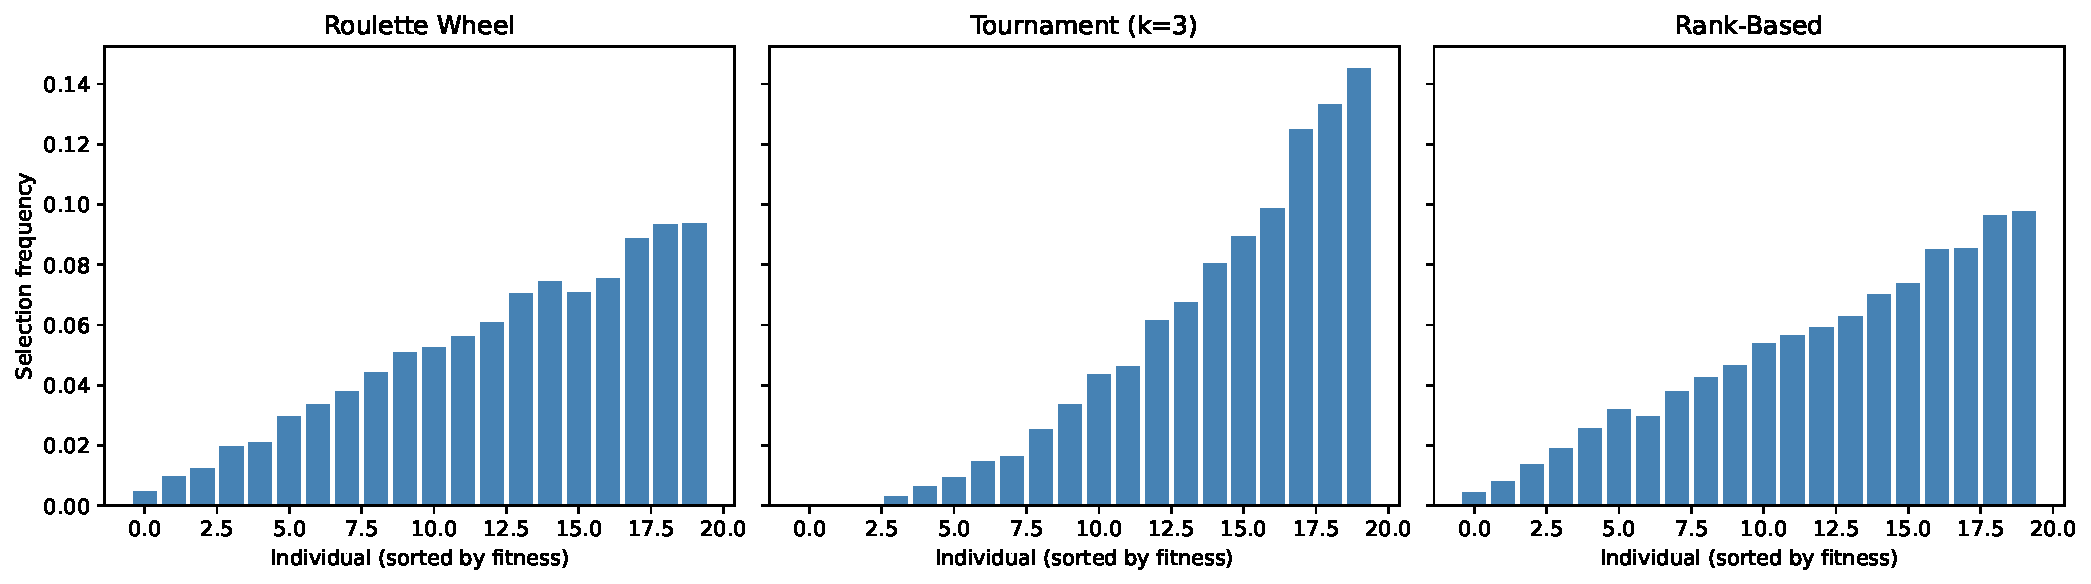
\includegraphics[width=0.7\linewidth]{files/5624b1f22ddca17724afcc6d1f9fb542.pdf}

FIGURE 11.2: Selection frequency for 20 individuals (sorted by increasing fitness) under three selection operators. Roulette wheel selection is proportional to absolute fitness, tournament selection concentrates more sharply on the fittest individuals, and rank-based selection depends only on ordinal position.

The results displayed in FIGURE 11.2 confirm that tournament selection offers the most convenient trade-off: it concentrates on high-fitness individuals without the extreme sensitivity to absolute fitness values that roulette wheel exhibits.

\paragraph{Demonstration: crossover operators compared}

To visualise how different crossover operators mix parental genetic material, we generate many children from two fixed parents and plot the resulting distributions.

\begin{verbatim}
L = 20
parent1 = np.zeros(L)          # All zeros
parent2 = np.ones(L)           # All ones
N_CHILDREN = 5_000

def single_point_xo(p1, p2):
    pt = random.randint(1, L - 1)
    return np.concatenate([p1[:pt], p2[pt:]])

def two_point_xo(p1, p2):
    pts = sorted(random.sample(range(1, L), 2))
    child = p1.copy()
    child[pts[0]:pts[1]] = p2[pts[0]:pts[1]]
    return child

def uniform_xo(p1, p2, p=0.5):
    mask = np.random.random(L) < p
    child = np.where(mask, p1, p2)
    return child

def arithmetic_xo(p1, p2, alpha=None):
    if alpha is None:
        alpha = random.random()
    return alpha * p1 + (1 - alpha) * p2

# Generate many children to see the distribution
operators = {
    "Single-point": single_point_xo,
    "Two-point": two_point_xo,
    "Uniform (p=0.5)": uniform_xo,
    "Arithmetic": arithmetic_xo
}

fig, axes = plt.subplots(1, 4, figsize=(16, 4), sharey=True)
for ax, (name, op) in zip(axes, operators.items()):
    sums = [op(parent1, parent2).sum() for _ in range(N_CHILDREN)]
    ax.hist(sums, bins=range(L + 2), density=True,
            color="steelblue", edgecolor="white")
    ax.set_title(name)
    ax.set_xlabel("Sum of child genes")
axes[0].set_ylabel("Density")
plt.suptitle("Crossover Operators: Child Gene-Sum Distributions",
             y=1.02)
plt.tight_layout()
plt.show()
\end{verbatim}

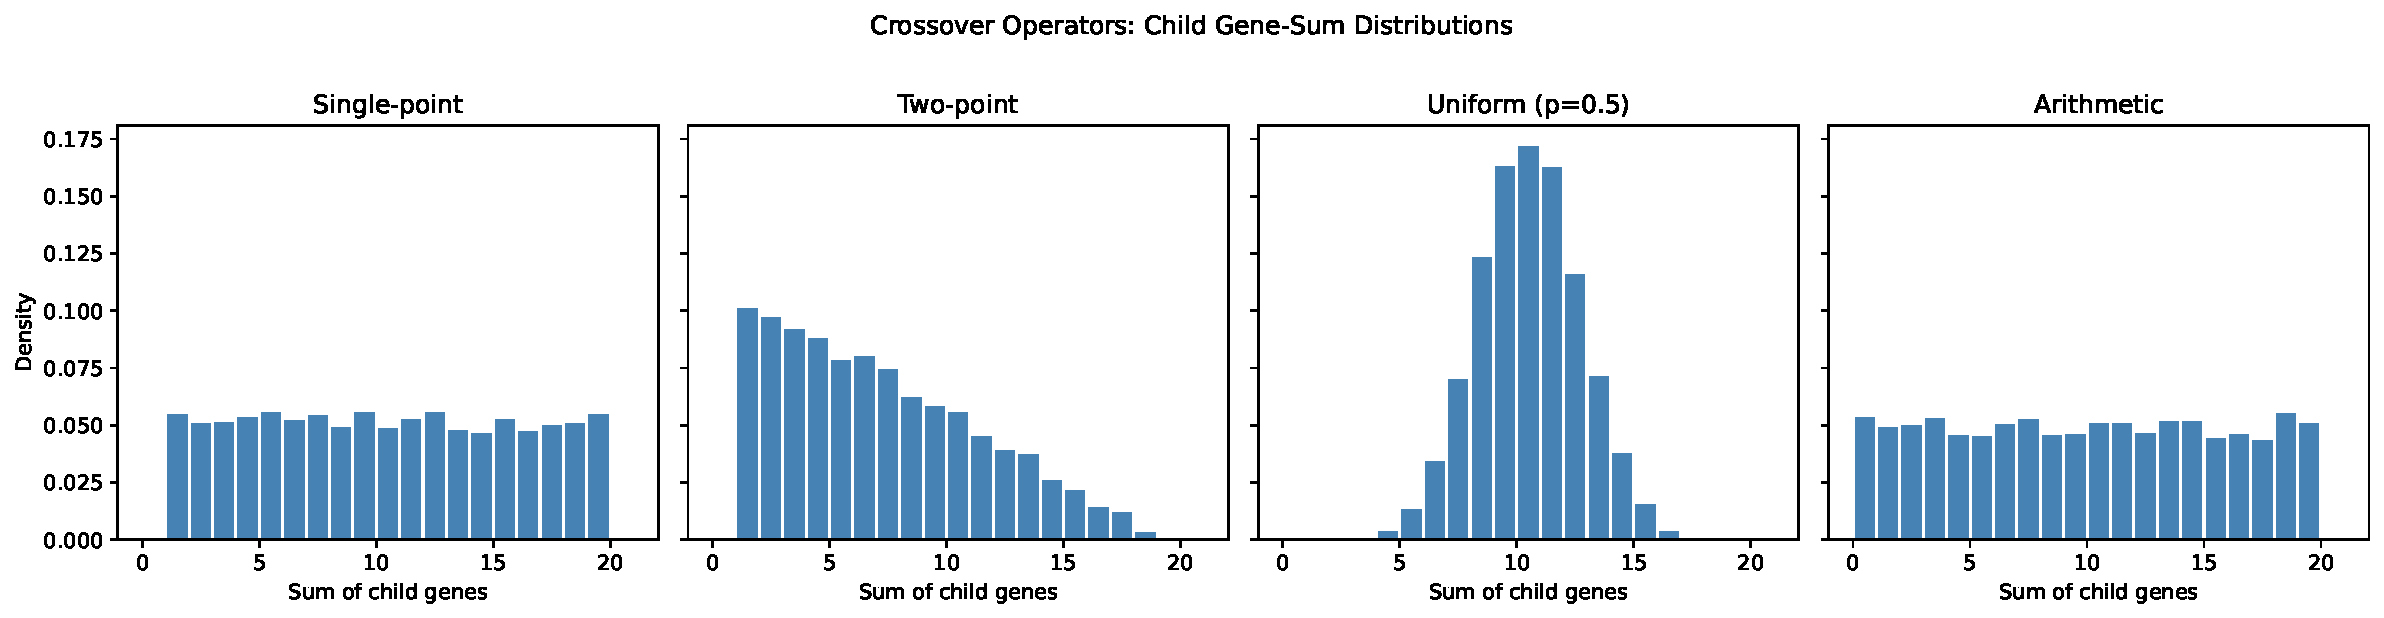
\includegraphics[width=0.7\linewidth]{files/e4bce44834f1c1c73b5cf1869f12f7c5.pdf}

FIGURE 11.3: Distribution of gene sums for children of an all-zeros parent and an all-ones parent. Single-point crossover produces a uniform distribution. Two-point crossover peaks at the extremes (when the swapped segment is short) and in the middle. Uniform crossover produces a binomial distribution centred at $L/2$. Arithmetic crossover yields a continuous uniform distribution on $[0, L]$.

FIGURE 11.3 reveals that the mixing behaviour differs substantially across operators. Uniform crossover is the most disruptive, while arithmetic crossover produces a continuous blend.

\paragraph{Demonstration: parameter sensitivity}

The interplay between population size and mutation rate is critical. We reuse the miniature feature-selection problem of §11.2.5 (its \texttt{fitness} function and standardised data), running it with varying settings and measuring convergence speed.

\begin{verbatim}
L = len(pool)            # restore pool size (the §11.3.8 demo reassigned L)

def run_fs_ga(pop_size, p_mut, n_gen=40, seed=42):
    """Run the feature-selection GA, return best-IC history."""
    np.random.seed(seed)
    random.seed(seed)
    pop = [np.random.randint(0, 2, size=L) for _ in range(pop_size)]
    hist = []
    for _ in range(n_gen):
        scores = [fitness(x) for x in pop]
        hist.append(max(scores))
        elite = pop[int(np.argmax(scores))].copy()
        children = [elite]
        while len(children) < pop_size:
            idx = random.sample(range(len(pop)), 3)
            p1 = pop[max(idx, key=lambda i: scores[i])].copy()
            idx = random.sample(range(len(pop)), 3)
            p2 = pop[max(idx, key=lambda i: scores[i])].copy()
            if random.random() < 0.9:
                pt = random.randint(1, L - 1)
                c = np.concatenate([p1[:pt], p2[pt:]])
            else:
                c = p1.copy()
            for j in range(L):
                if random.random() < p_mut:
                    c[j] = 1 - c[j]
            children.append(c)
        pop = children[:pop_size]
    return hist

# -- Experiment 1: Population size ----------------------------
fig, axes = plt.subplots(1, 2, figsize=(14, 5))
for ps in [10, 20, 50, 100, 200]:
    h = run_fs_ga(pop_size=ps, p_mut=1.0 / L)
    axes[0].plot(h, label=f"N={ps}")
axes[0].set_xlabel("Generation")
axes[0].set_ylabel("Best composite IC")
axes[0].set_title("Effect of population size (p_mut=1/L)")
axes[0].legend()

# -- Experiment 2: Mutation rate ------------------------------
for pm in [0.01, 0.05, 0.07, 0.14, 0.30]:
    h = run_fs_ga(pop_size=50, p_mut=pm)
    axes[1].plot(h, label=f"p_m={pm}")
axes[1].set_xlabel("Generation")
axes[1].set_ylabel("Best composite IC")
axes[1].set_title("Effect of mutation rate (N=50)")
axes[1].legend()
plt.tight_layout()
plt.show()
\end{verbatim}

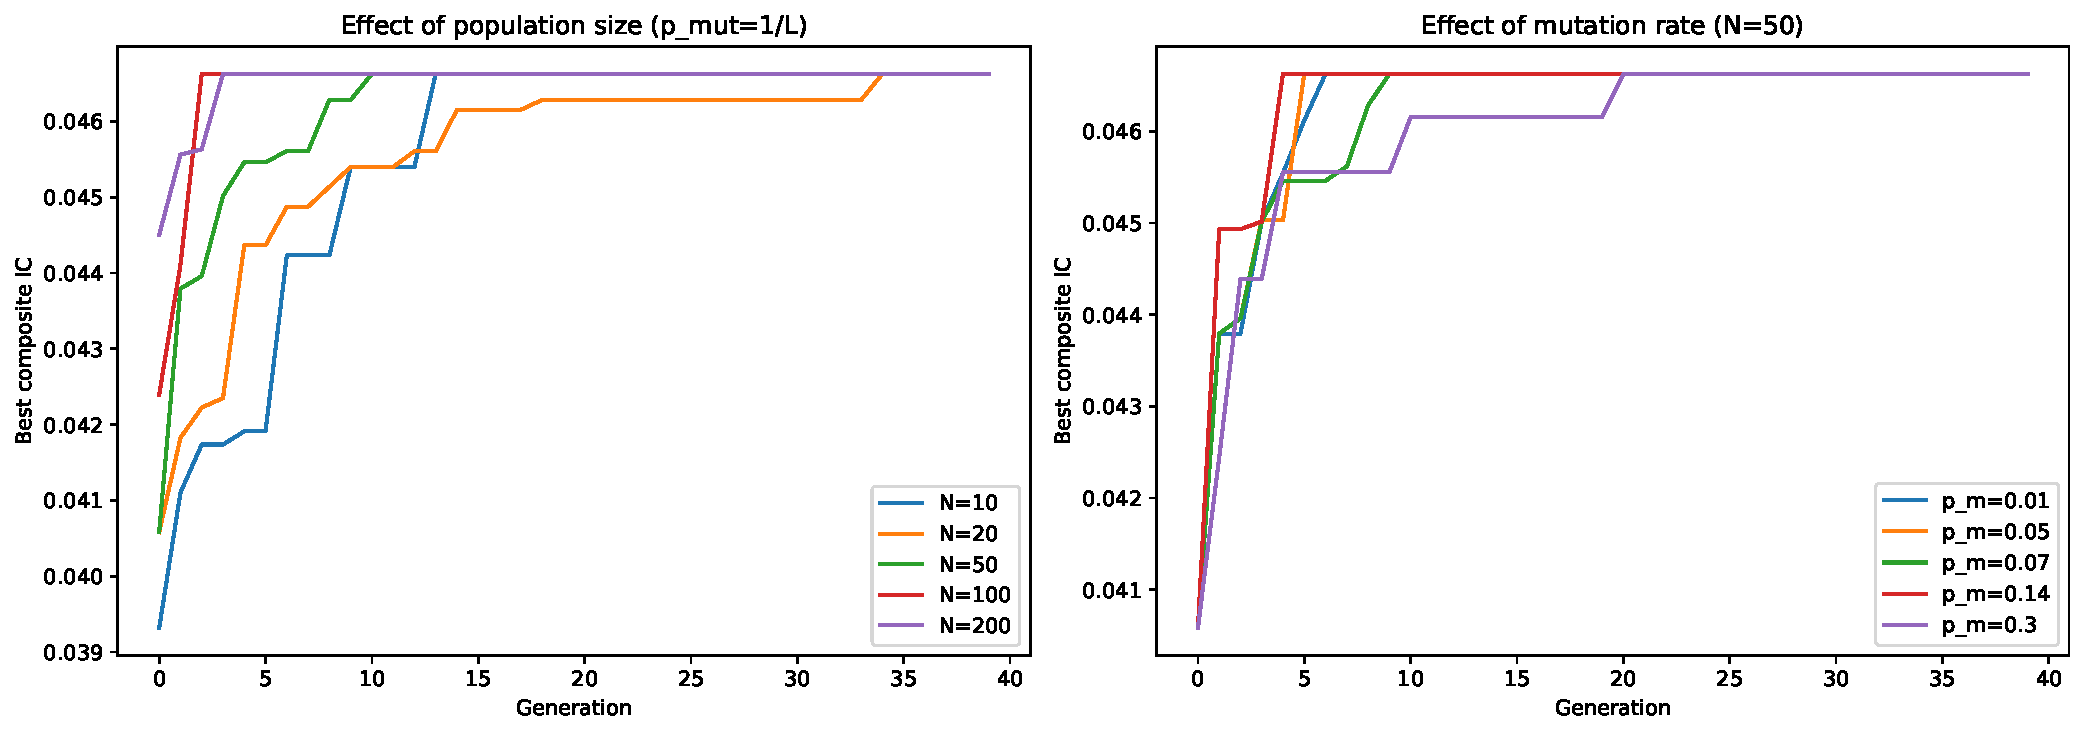
\includegraphics[width=0.7\linewidth]{files/098cf737d40550611ed2229d4b06b051.pdf}

FIGURE 11.4: \textbf{Left:} Larger populations converge faster to the optimal composite IC (about 0.047) thanks to greater initial diversity, with $N = 100$ and $N = 200$ almost indistinguishable, showing diminishing returns beyond $N \approx 100$. \textbf{Right:} Mutation rates near $1/L$ to $2/L$ (0.07 to 0.14) converge fastest; a very high rate ($p_m = 0.30$) is disruptive and reaches the optimum more slowly, while a very low rate ($p_m = 0.01$) is also slower to escape early plateaus. The intermediate values offer the best trade-off.

The results, shown in FIGURE 11.4, confirm a well-known guideline: a population of 50 to 100 with a mutation rate of $1/L$ to $2/L$ is a robust starting point for binary-encoded problems.

\subsubsection{Applications in factor investing}

We now turn to the primary motivation for this chapter: applying GAs across the systematic factor-investing workflow. The four core applications follow that workflow in order: \textbf{selecting} which features enter a model (§11.4.1), \textbf{constructing} a constrained portfolio from them (§11.4.2), \textbf{tuning} the model that maps features to forecasts (§11.4.3), and \textbf{discovering} entirely new alpha factors from raw data (§11.4.4). Each is accompanied by a complete code example on the book dataset. A final section (§11.4.5) surveys three research frontiers, trading-rule evolution, neuroevolution, and LLM-GA hybrids, where evolutionary methods are actively reshaping quantitative investing but which sit further from the core feature-selection problem.

\paragraph{Feature selection with GA}

Feature selection was briefly introduced in Chapter 5 (§5.4.1) as a preprocessing step. The challenge is to select, from a universe of $K$ candidate features, a subset that maximises predictive performance while avoiding overfitting. This is a combinatorial problem with $2^K$ possible subsets.

GAs are a natural \textbf{wrapper method} for feature selection: each chromosome is a binary mask of length $K$, and the fitness function is the cross-validated performance of a predictive model trained on the selected features. \cite{Dokeroglu2022} conducted a comprehensive survey confirming that GAs are the most widely used metaheuristic for feature selection. \cite{deBarros2024} recently demonstrated the effectiveness of GA-based feature selection specifically for financial time series, achieving improved monotonicity prediction through principled feature subset discovery. Closer still to our own setting, \cite{Kottas2026} couples a GA with a learning-to-rank objective to construct US equity portfolios, ranking stocks on GA-selected characteristics before allocation, a direct analogue of the pipeline we develop in §11.6.

We use the DEAP library (Distributed Evolutionary Algorithms in Python) of \cite{Fortin2012} to implement a GA that selects features for an XGBoost classifier (introduced in Chapter 7). We apply it directly to the book's US equity panel, the full dataset described in §11.6: 122 candidate features and a binary target equal to one when a stock's next-month return exceeds the cross-sectional median for that month. To keep the demonstration fast we draw a random sample of 4,000 stock-months from a 2015 to 2019 in-sample window; the rigorous walk-forward evaluation is deferred to §11.6.

\begin{verbatim}
import numpy as np
import random
import xgboost as xgb
from deap import base, creator, tools, algorithms
import pandas as pd
from sklearn.model_selection import cross_val_score, StratifiedKFold

# -- Reproducibility ------------------------------------------
SEED = 42
np.random.seed(SEED)
random.seed(SEED)

# -- Data: the book US equity panel (see §11.6) ---------------
data_ml = pd.read_parquet('data/mlfi_us_data.parquet')
data_ml = data_ml.rename(columns={'id': 'stock_id'})
exclude = ['stock_id', 'date', 'R1M_Usd', 'R3M_Usd', 'R6M_Usd',
           'R12M_Usd']
feature_names = [c for c in data_ml.columns if c not in exclude]
n_features = len(feature_names)             # 122 candidate features

# Binary label: beat the cross-sectional median next-month return
win = data_ml[data_ml['date'].between('2015-01-01', '2019-12-31')]
win = win.dropna(subset=['R1M_Usd'])
med = win.groupby('date')['R1M_Usd'].transform('median')
win = win.assign(label=(win['R1M_Usd'] > med).astype(int))
sample = win.sample(n=4000, random_state=SEED)
X = sample[feature_names].values
y = sample['label'].values
feature_names = np.array(feature_names)
cv = StratifiedKFold(n_splits=5, shuffle=True, random_state=SEED)

# -- Fitness function -----------------------------------------
def evaluate(individual):
    """CV AUC of XGBoost using selected features."""
    mask = np.array(individual, dtype=bool)
    if mask.sum() == 0:                      # No features selected
        return (0.0,)
    model = xgb.XGBClassifier(
        n_estimators=40, max_depth=3, learning_rate=0.1,
        tree_method="hist", random_state=SEED,
        verbosity=0, n_jobs=-1)
    scores = cross_val_score(
        model, X[:, mask], y, cv=cv, scoring="roc_auc")
    return (scores.mean(),)                  # Must return a tuple

# -- DEAP setup -----------------------------------------------
# Create fitness and individual types
creator.create("FitnessMax", base.Fitness, weights=(1.0,))
creator.create("Individual", list, fitness=creator.FitnessMax)

toolbox = base.Toolbox()
toolbox.register("attr_bool", random.randint, 0, 1)
toolbox.register("individual", tools.initRepeat,
                 creator.Individual, toolbox.attr_bool,
                 n=n_features)
toolbox.register("population", tools.initRepeat,
                 list, toolbox.individual)
toolbox.register("evaluate", evaluate)
toolbox.register("mate", tools.cxUniform, indpb=0.5)
toolbox.register("mutate", tools.mutFlipBit, indpb=1/n_features)
toolbox.register("select", tools.selTournament, tournsize=3)

# -- Run GA ---------------------------------------------------
pop = toolbox.population(n=24)              # 24 individuals
hof = tools.HallOfFame(1)                   # Track best ever
stats = tools.Statistics(lambda ind: ind.fitness.values)
stats.register("max", np.max)
stats.register("avg", np.mean)

pop, logbook = algorithms.eaSimple(
    pop, toolbox,
    cxpb=0.7,                               # Crossover probability
    mutpb=0.2,                               # Mutation probability
    ngen=12,                                 # Number of generations
    stats=stats, halloffame=hof, verbose=False)

# -- Results --------------------------------------------------
best = hof[0]
mask = np.array(best, dtype=bool)
print(f"Selected {mask.sum()} / {n_features} features")
print(f"Best CV AUC: {best.fitness.values[0]:.4f}")

# -- Compare with using ALL features --------------------------
model_all = xgb.XGBClassifier(
    n_estimators=40, max_depth=3, learning_rate=0.1,
    tree_method="hist", random_state=SEED,
    verbosity=0, n_jobs=-1)
auc_all = cross_val_score(
    model_all, X, y, cv=cv, scoring="roc_auc").mean()
print(f"AUC with ALL features: {auc_all:.4f}")
\end{verbatim}

\begin{verbatim}
Selected 60 / 122 features
Best CV AUC: 0.5305
AUC with ALL features: 0.5010
\end{verbatim}

The GA selects 60 of the 122 features and lifts the cross-validated AUC from 0.501 (all features) to 0.530. Two points deserve emphasis. First, the absolute AUC is low: predicting the sign of next-month returns from firm characteristics is genuinely hard, and an AUC near 0.53 is typical for monthly cross-sectional equity classification. Second, and despite this, discarding roughly half the features produces a clear relative improvement, precisely because many of the 122 characteristics are redundant or noisy and the full-feature model dilutes signal with them. The selected subset is dominated by profitability, value, and earnings-quality measures (for example \texttt{ROA}, \texttt{ROIC}, \texttt{EV\_EBITDA}, and \texttt{REV\_Quarterly\_Surprise}), together with a handful of liquidity, volatility, and momentum signals (\texttt{idio\_vol\_252d}, \texttt{adv\_252}, \texttt{mom\_252}), echoing the factor categories that decades of research have found to matter. This advantage becomes more pronounced when $K$ is large relative to the training sample size, precisely the situation encountered here with 122 characteristics. We caution that this single in-sample window is illustrative only; §11.6 evaluates GA feature selection under a proper walk-forward protocol.

\textbf{From selection to weighted composites.} Binary feature selection sits at one end of a continuum. At the other end lies full genetic programming (§11.4.4), which evolves arbitrary expressions over the feature set. In between lies a practical and powerful middle ground: \textbf{weighted feature composites}, where the GA simultaneously selects features and assigns them real-valued combination weights. The chromosome becomes a hybrid: a binary gene for inclusion and a continuous gene for the weight of each feature. The arithmetic crossover of Equation (11.4) applies to the weight portion, while bit-flip mutation handles the binary portion. This generalises the binary encoding demonstrated above in a natural way that the DEAP framework supports directly (one need only register two attribute generators, one binary and one float, and concatenate them into a single individual).

Why do weights matter? The equal-weighted composite used in our empirical application (§11.6) treats all selected features as equally informative. In practice, momentum and value signals differ in predictive strength, noise level, and decay rate. \cite{reschenhofer2024combining} estimates optimal factor-combination weights for small-cap stocks (roughly 36\% value, 28\% momentum, 11\% profitability, and 5\% investment), while cautioning that simple equal-weighting of the factors remains a hard-to-beat benchmark in practice. AlphaGen \citep{Yu2023} goes further by optimising for \textit{synergy} among factors: the reward signal is the combined portfolio's performance, not individual factor quality. This aligns with the ensemble combination ideas of Chapter 13, where the optimal aggregation of weak learners is rarely uniform.

AlphaForge \citep{Shi2025} extends this to \textbf{time-varying weights}, dynamically adjusting each factor's contribution at each rebalancing date. The resulting composite adapts to market regime changes (the COVID-19 dislocation discussed in §11.6.3 is a case in point). We note that evolving time-varying weights requires either a richer chromosome (one weight per factor per regime) or a two-stage approach: GA for feature selection, followed by a downstream model for dynamic weighting. Exercise 3 at the end of this chapter provides an opportunity to implement the simpler static-weight variant.

\paragraph{Portfolio optimisation with cardinality constraints}

The classical \cite{markowitz1952portfolio} mean-variance optimisation selects the portfolio $\mathbf{w}^*$ that minimises variance for a target return, or equivalently maximises the Sharpe ratio:

\begin{equation}
\mathbf{w}^* = \arg\max_{\mathbf{w}} \frac{\mathbf{w}^\top \boldsymbol{\mu} - r_f}{\sqrt{\mathbf{w}^\top \boldsymbol{\Sigma} \mathbf{w}}}, \qquad \text{s.t.} \quad \sum_n w_n = 1, \quad w_n \geq 0. \tag{11.5}
\end{equation}

This is a quadratic program and can be solved exactly. However, adding a \textbf{cardinality constraint} $\|\mathbf{w}\|_0 \leq K_{\max}$ (hold at most $K_{\max}$ assets) renders the problem NP-hard \citep{Chang2000}. With $N = 500$ assets and $K_{\max} = 30$, the number of possible asset subsets is $\binom{500}{30} \approx 10^{42}$, which is beyond exhaustive enumeration.

A GA handles this naturally. Zhang, Y. et al. (2024) demonstrate that evolutionary approaches (including memetic algorithms that combine GA-based global search with local refinement) outperform classical factor analysis methods for portfolio optimisation under such constraints. Before we proceed to the implementation, it is useful to note that three paradigms for handling constraints in evolutionary algorithms are common in the literature:

\begin{itemize}
\item \textbf{Penalty functions} add a term to the fitness that penalises constraint violations (as in Equation 11.2 for feature selection). This is flexible but requires tuning the penalty weight $\lambda$: too small and infeasible solutions dominate the population; too large and the search avoids the constraint boundary where optima often lie.
\item \textbf{Repair operators} project infeasible solutions back into the feasible region after crossover and mutation. Weight normalisation (dividing by the sum) and zeroing-out of small weights are both repair approaches. Repair preserves genetic information while enforcing feasibility, but the projection can introduce bias toward certain regions of the feasible space.
\item \textbf{Decoder approaches} use an indirect encoding where the chromosome is mapped to a feasible solution by construction. For example, a chromosome of $N$ real values can be decoded to portfolio weights via softmax normalisation, guaranteeing $\sum_n w_n = 1$ and $w_n \geq 0$ without explicit constraints.
\end{itemize}

In practice, combining repair operators with mild penalty functions is often effective \citep{Chang2000}. Our implementation below uses repair (normalisation) for the budget constraint and penalty for the cardinality constraint. We encode the chromosome as a real-valued vector of length $N$. Assets with weights below a threshold $\epsilon$ are zeroed out, and the remaining weights are renormalised. The cardinality constraint is enforced by zeroing the smallest weights if too many assets are selected.

\begin{verbatim}
import numpy as np
import random
from deap import base, creator, tools, algorithms
import matplotlib.pyplot as plt

# -- Reproducibility ------------------------------------------
SEED = 42
np.random.seed(SEED)
random.seed(SEED)

# -- Real returns: 30 most liquid stocks, 2015 -2019 window ----
import pandas as pd
data_ml = pd.read_parquet('data/mlfi_us_data.parquet')
data_ml = data_ml.rename(columns={'id': 'stock_id'})
win = data_ml[data_ml['date'].between('2015-01-01', '2019-12-31')]
returns = win.pivot_table(index='date', columns='stock_id',
                          values='R1M_Usd').dropna(axis=1)
liq = win.groupby('stock_id')['adv_252'].mean()
top = liq[returns.columns].sort_values(ascending=False).head(30).index
R = returns[top]                          # 30 x 60 monthly return panel

N_ASSETS = 30
K_MAX = 8                                 # Maximum holdings
mu = R.mean().values                      # Mean monthly returns
Sigma = R.cov().values                    # Return covariance matrix
rf = 0.0                                  # Monthly risk-free rate

# -- Fitness function -----------------------------------------
def evaluate_portfolio(individual):
    """Sharpe ratio with cardinality constraint."""
    w = np.array(individual)
    w = np.maximum(w, 0)                   # Long-only

    # Enforce cardinality: keep only top K_MAX weights
    if (w > 1e-6).sum() > K_MAX:
        threshold = np.sort(w)[-K_MAX]
        w[w < threshold] = 0

    if w.sum() < 1e-10:
        return (-10.0,)                    # Penalise empty portfolio

    w = w / w.sum()                        # Normalise to sum to 1

    port_return = w @ mu
    port_vol = np.sqrt(w @ Sigma @ w)
    sharpe = (port_return - rf) / port_vol if port_vol > 0 else 0
    return (sharpe,)

# -- DEAP setup -----------------------------------------------
creator.create("FitMax", base.Fitness, weights=(1.0,))
creator.create("Ind", list, fitness=creator.FitMax)

toolbox = base.Toolbox()
toolbox.register("gene", random.random)
toolbox.register("individual", tools.initRepeat,
                 creator.Ind, toolbox.gene, n=N_ASSETS)
toolbox.register("population", tools.initRepeat,
                 list, toolbox.individual)
toolbox.register("evaluate", evaluate_portfolio)
toolbox.register("mate", tools.cxBlend, alpha=0.3)
toolbox.register("mutate", tools.mutGaussian,
                 mu=0, sigma=0.1, indpb=0.2)
toolbox.register("select", tools.selTournament, tournsize=3)

# -- Run GA ---------------------------------------------------
pop = toolbox.population(n=100)
hof = tools.HallOfFame(1)
stats = tools.Statistics(lambda ind: ind.fitness.values)
stats.register("max", np.max)
stats.register("avg", np.mean)

pop, logbook = algorithms.eaSimple(
    pop, toolbox, cxpb=0.6, mutpb=0.3,
    ngen=80, stats=stats, halloffame=hof, verbose=False)

# -- Extract best portfolio -----------------------------------
best_w = np.array(hof[0])
best_w = np.maximum(best_w, 0)
if (best_w > 1e-6).sum() > K_MAX:
    threshold = np.sort(best_w)[-K_MAX]
    best_w[best_w < threshold] = 0
best_w = best_w / best_w.sum()

print(f"Number of holdings: {(best_w > 1e-6).sum()}")
print(f"Sharpe (monthly): {hof[0].fitness.values[0]:.3f}")
print(f"Expected monthly return: {best_w @ mu:.3%}")
print(f"Monthly volatility: {np.sqrt(best_w @ Sigma @ best_w):.3%}")
print(f"Annualised Sharpe: {hof[0].fitness.values[0] * np.sqrt(12):.3f}")
\end{verbatim}

\begin{verbatim}
Number of holdings: 8
Sharpe (monthly): 0.565
Expected monthly return: 2.058%
Monthly volatility: 3.644%
Annualised Sharpe: 1.957
\end{verbatim}

\begin{verbatim}
# -- Plot convergence and portfolio ---------------------------
fig, axes = plt.subplots(1, 2, figsize=(14, 5))

# Convergence
gen = logbook.select("gen")
fit_max = logbook.select("max")
fit_avg = logbook.select("avg")
axes[0].plot(gen, fit_max, label="Best Sharpe", linewidth=2)
axes[0].plot(gen, fit_avg, label="Avg Sharpe",
             linestyle="--")
axes[0].set_xlabel("Generation")
axes[0].set_ylabel("Sharpe ratio")
axes[0].set_title("Convergence")
axes[0].legend()

# Portfolio weights
nonzero = best_w > 1e-6
axes[1].bar(np.where(nonzero)[0], best_w[nonzero],
            color="steelblue")
axes[1].set_xlabel("Asset index")
axes[1].set_ylabel("Weight")
axes[1].set_title(f"Optimal Portfolio ({(nonzero).sum()} assets)")
plt.tight_layout()
plt.show()
\end{verbatim}

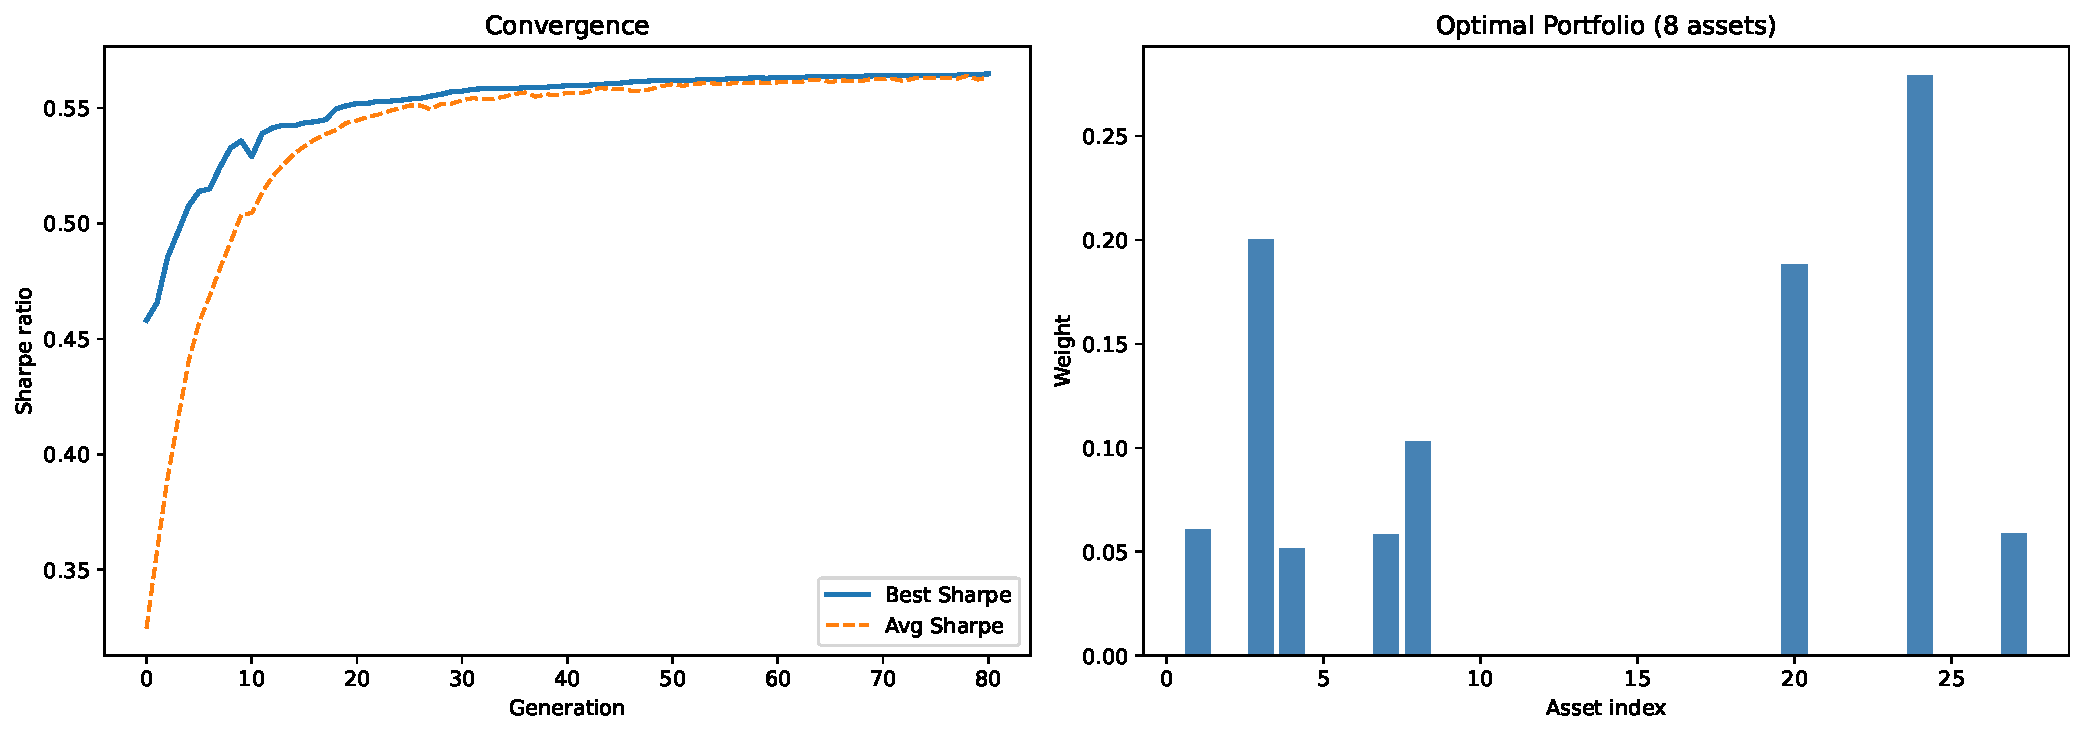
\includegraphics[width=0.7\linewidth]{files/e6e8489eb9fad7ea97e1ff311834bd82.pdf}

FIGURE 11.5: \textbf{Left:} GA convergence for cardinality-constrained portfolio optimisation on 30 real US equities (2015 to 2019). The best monthly Sharpe ratio stabilises well before the 80th generation. \textbf{Right:} The optimal portfolio weights, concentrated in 8 of the 30 candidate stocks, as enforced by the cardinality constraint $K_{\max} = 8$.

FIGURE 11.5 illustrates both the convergence dynamics and the resulting portfolio. The GA concentrates the portfolio in exactly $K_{\max} = 8$ of the 30 candidate stocks while achieving a monthly Sharpe ratio of 0.57 (roughly 1.96 annualised). This would be impressive in practice, but it must be viewed with great caution: the expected returns and covariances are estimated in-sample over the same 2015 to 2019 window, so the figure reflects optimisation over realised history rather than genuine out-of-sample skill.

\paragraph{Hyperparameter tuning with GA}

Chapter 12 (§12.3) introduced grid search and Bayesian optimisation for hyperparameter tuning. GAs offer a third approach that is particularly attractive when the hyperparameter space is mixed (some continuous, some discrete, some conditional).

We demonstrate by tuning XGBoost hyperparameters using a GA. The chromosome is a real-valued vector of 10 genes, each representing one hyperparameter normalised to $[0, 1]$ and then mapped to its actual range. We deliberately search a fairly rich space, ten parameters including three regularisation terms, over a long training history (2004 to 2014), because this is the regime in which evolutionary search has a genuine edge over simpler alternatives, as we discuss below.

\begin{verbatim}
import numpy as np
import random
import xgboost as xgb
from deap import base, creator, tools, algorithms
import pandas as pd
from sklearn.model_selection import cross_val_score, StratifiedKFold

SEED = 42
np.random.seed(SEED)
random.seed(SEED)

# Book US equity panel; predict the sign of next-month returns
data_ml = pd.read_parquet('data/mlfi_us_data.parquet')
data_ml = data_ml.rename(columns={'id': 'stock_id'})
# 20 characteristics spanning momentum, value, quality, and volatility
features = ['REV_Quarterly_Surprise', 'Buyback_Yield', 'mom_22', 'rsi_14',
            'EPS_Quarterly_Surprise', 'Book_Value_PS', 'vol_22', 'vol_66',
            'Asset_Growth_1Y', 'Div_yld', 'abn_volume_21', 'Net_Income_to_CFO',
            'EPS_FY1_Rev30d', 'skew_252', 'Fixed_Asset_Turnover', 'kurt_252',
            'Sales_Growth_3Y', 'Capex_Intensity', 'FCF_yld', 'rel_str_252d']
win = data_ml[data_ml['date'].between('2004-01-01', '2014-12-31')]
win = win.dropna(subset=features + ['R1M_Usd'])
med = win.groupby('date')['R1M_Usd'].transform('median')
win = win.assign(label=(win['R1M_Usd'] > med).astype(int))
sample = win.sample(n=10000, random_state=SEED)
X = sample[features].values
y = sample['label'].values
cv = StratifiedKFold(n_splits=5, shuffle=True, random_state=SEED)

# -- Hyperparameter space (10 genes, including 3 regularisers) -
def decode(individual):
    """Map [0,1]^10 genes to XGBoost hyperparameters."""
    g = np.clip(individual, 0, 1)
    return dict(
        n_estimators=int(50 + g[0] * 350),    # 50-400
        max_depth=int(2 + g[1] * 8),           # 2-10
        learning_rate=0.01 + g[2] * 0.29,      # 0.01-0.30
        subsample=0.5 + g[3] * 0.5,            # 0.5-1.0
        colsample_bytree=0.4 + g[4] * 0.6,     # 0.4-1.0
        min_child_weight=int(1 + g[5] * 9),    # 1-10
        reg_alpha=g[6] * 5.0,                  # L1 penalty, 0-5
        reg_lambda=g[7] * 5.0,                 # L2 penalty, 0-5
        gamma=g[8] * 5.0,                      # min split loss, 0-5
        colsample_bylevel=0.4 + g[9] * 0.6     # 0.4-1.0
    )

def evaluate_hp(individual):
    """5-fold CV AUC for decoded hyperparameters."""
    params = decode(individual)
    model = xgb.XGBClassifier(
        **params, tree_method="hist", random_state=SEED,
        verbosity=0, n_jobs=-1)
    scores = cross_val_score(
        model, X, y, cv=cv, scoring="roc_auc")
    return (scores.mean(),)

# -- DEAP setup -----------------------------------------------
creator.create("FitHP", base.Fitness, weights=(1.0,))
creator.create("IndHP", list, fitness=creator.FitHP)

toolbox = base.Toolbox()
toolbox.register("gene", random.random)
toolbox.register("individual", tools.initRepeat,
                 creator.IndHP, toolbox.gene, n=10)
toolbox.register("population", tools.initRepeat,
                 list, toolbox.individual)
toolbox.register("evaluate", evaluate_hp)
toolbox.register("mate", tools.cxBlend, alpha=0.3)
toolbox.register("mutate", tools.mutGaussian,
                 mu=0, sigma=0.15, indpb=0.3)
toolbox.register("select", tools.selTournament, tournsize=3)

# -- Run GA ---------------------------------------------------
pop = toolbox.population(n=24)
hof = tools.HallOfFame(1)

pop, logbook = algorithms.eaSimple(
    pop, toolbox, cxpb=0.6, mutpb=0.3,
    ngen=40, halloffame=hof, verbose=False)

best_params = decode(hof[0])
print(f"Best CV AUC: {hof[0].fitness.values[0]:.4f}")
print(f"Best hyperparameters: {best_params}")

# -- Random search baseline (matched budget) ------------------
best_random = 0
for _ in range(24 * 40):     # Same total evaluations as GA
    ind = [random.random() for _ in range(10)]
    auc = evaluate_hp(ind)[0]
    if auc > best_random:
        best_random = auc
print(f"Best random search AUC: {best_random:.4f}")
\end{verbatim}

\begin{verbatim}
Best CV AUC: 0.5335
Best hyperparameters: {'n_estimators': 261, 'max_depth': 8,
  'learning_rate': 0.125, 'subsample': 0.738,
  'colsample_bytree': 0.400, 'min_child_weight': 6,
  'reg_alpha': 3.789, 'reg_lambda': 2.231, 'gamma': 5.000,
  'colsample_bylevel': 0.730}
Best random search AUC: 0.5294
\end{verbatim}

Given the same total budget of fitness evaluations (population $\times$ generations for the GA, an equal number of random trials), the GA attains a cross-validated AUC of 0.534, against 0.529 for random search. The reason the GA wins here, when over a compact space of only a handful of parameters random sampling is famously hard to beat \citep{bergstra2012random}, is dimensionality: with ten hyperparameters the space is sparse enough that a fixed budget of random draws leaves gaps, whereas the GA's crossover and selection exploit the interactions between parameters (for example the interplay of learning rate, tree depth, and the three regularisation terms) to home in on a stronger region. The winning configuration is heavily regularised, a moderate learning rate combined with large \texttt{reg\_alpha}, \texttt{reg\_lambda}, and \texttt{gamma} penalties and aggressive column subsampling, which is the profile one expects for a high-noise target. The advantage is modest in absolute terms, as it must be at the signal-to-noise ratio of monthly cross-sectional returns, but it is genuine and it widens with the dimensionality of the search, precisely the regime in which a GA repays its extra cost over grid or random search. The more consequential lesson, that the configuration maximising in-sample fitness need not generalise, is developed in §11.6.5, where a naive in-sample fitness overfits, while a fitness aligned with out-of-sample performance lets the GA-tuned model beat its baselines.

\paragraph{Alpha factor discovery with genetic programming}

Genetic programming extends the GA framework from fixed-length vectors to variable-length \textbf{expression trees}. In factor investing, GP can discover new formulaic alphas by composing primitive operators and market data fields. This approach was formalised at scale by \cite{Kakushadze2016} with his ``101 Formulaic Alphas.''

We demonstrate GP by mining a formulaic alpha directly on the book dataset. The terminals are six standardised firm characteristics, the primitives are the four arithmetic operators (with protected division), and the fitness is the cross-sectional \textbf{Information Coefficient} (IC): the Spearman rank correlation between the tree's output and the next-month return. Maximising IC is precisely the objective a quantitative researcher cares about.

\begin{verbatim}
import operator
import numpy as np
import pandas as pd
import random
from deap import base, creator, tools, gp, algorithms
from scipy.stats import spearmanr

SEED = 42
np.random.seed(SEED)
random.seed(SEED)

# -- Data: six standardised features, target = next-month return
data_ml = pd.read_parquet('data/mlfi_us_data.parquet')
data_ml = data_ml.rename(columns={'id': 'stock_id'})
gp_feats = ['mom_252', 'vol_252', 'size_log', 'PB', 'ROE', 'Div_yld']
d = data_ml[data_ml['date'].between('2015-01-01', '2019-12-31')]
d = d.dropna(subset=gp_feats + ['R1M_Usd']).copy()
for f in gp_feats:                          # cross-sectional z-score
    g = d.groupby('date')[f]
    d[f] = ((d[f] - g.transform('mean')) /
            g.transform('std')).fillna(0.0).clip(-5, 5)
Xz = [d[f].values for f in gp_feats]
y = d['R1M_Usd'].values

# -- Protected division (closure) ------------------------------
def safe_div(a, b):
    b = np.asarray(b, dtype=float)
    return np.where(np.abs(b) > 1e-6, a / np.where(b == 0, 1, b), 1.0)

# -- Primitive set: 6 feature terminals + arithmetic -----------
pset = gp.PrimitiveSet("MAIN", arity=len(gp_feats))
pset.addPrimitive(np.add, 2)
pset.addPrimitive(np.subtract, 2)
pset.addPrimitive(np.multiply, 2)
pset.addPrimitive(safe_div, 2)
pset.addEphemeralConstant("rc", lambda: round(random.uniform(-2, 2), 2))
pset.renameArguments(**{f"ARG{i}": nm for i, nm in enumerate(gp_feats)})

# -- DEAP setup: maximise cross-sectional IC -------------------
creator.create("FitIC", base.Fitness, weights=(1.0,))
creator.create("IndTree", gp.PrimitiveTree, fitness=creator.FitIC)

toolbox = base.Toolbox()
toolbox.register("expr", gp.genHalfAndHalf, pset=pset, min_=1, max_=3)
toolbox.register("individual", tools.initIterate,
                 creator.IndTree, toolbox.expr)
toolbox.register("population", tools.initRepeat, list, toolbox.individual)
toolbox.register("compile", gp.compile, pset=pset)

def eval_ic(individual):
    func = toolbox.compile(expr=individual)
    pred = np.asarray(func(*Xz), dtype=float)
    if pred.ndim == 0 or not np.isfinite(pred).all() or pred.std() < 1e-12:
        return (-1.0,)                       # reject degenerate trees
    ic, _ = spearmanr(pred, y)
    return (ic if np.isfinite(ic) else -1.0,)

toolbox.register("evaluate", eval_ic)
toolbox.register("select", tools.selTournament, tournsize=5)
toolbox.register("mate", gp.cxOnePoint)
toolbox.register("expr_mut", gp.genFull, min_=0, max_=2)
toolbox.register("mutate", gp.mutUniform, expr=toolbox.expr_mut, pset=pset)
toolbox.decorate("mate",
                 gp.staticLimit(operator.attrgetter("height"), 6))
toolbox.decorate("mutate",
                 gp.staticLimit(operator.attrgetter("height"), 6))

# -- Run GP ----------------------------------------------------
pop = toolbox.population(n=200)
hof = tools.HallOfFame(1)
pop, logbook = algorithms.eaSimple(
    pop, toolbox, cxpb=0.7, mutpb=0.2, ngen=25,
    halloffame=hof, verbose=False)

# -- Results ---------------------------------------------------
best_tree = hof[0]
print(f"Discovered alpha: {best_tree}")
print(f"Pooled IC: {best_tree.fitness.values[0]:.4f}")

singles = {f: spearmanr(d[f].values, y)[0] for f in gp_feats}
bf = max(singles, key=lambda k: abs(singles[k]))
print(f"Best single-feature IC: {bf} = {singles[bf]:.4f}")
\end{verbatim}

\begin{verbatim}
Discovered alpha: subtract(add(subtract(subtract(PB,
  multiply(add(vol_252, vol_252), 0.24)), size_log), 0.03),
  add(vol_252, Div_yld))
Pooled IC: 0.0446
Best single-feature IC: PB = 0.0248
\end{verbatim}

\begin{verbatim}
import matplotlib.pyplot as plt

func = toolbox.compile(expr=best_tree)
pred = np.asarray(func(*Xz), dtype=float)
dec = pd.qcut(pd.Series(pred).rank(method="first"), 10, labels=False)
mean_ret = pd.Series(y).groupby(dec).mean()

fig, ax = plt.subplots(figsize=(8, 5))
ax.bar(mean_ret.index + 1, mean_ret.values, color="steelblue")
ax.set_xlabel("Predicted-alpha decile (1 = low, 10 = high)")
ax.set_ylabel("Mean realised next-month return")
ax.set_title("GP-discovered alpha: monotonicity across deciles")
plt.tight_layout()
plt.show()
\end{verbatim}

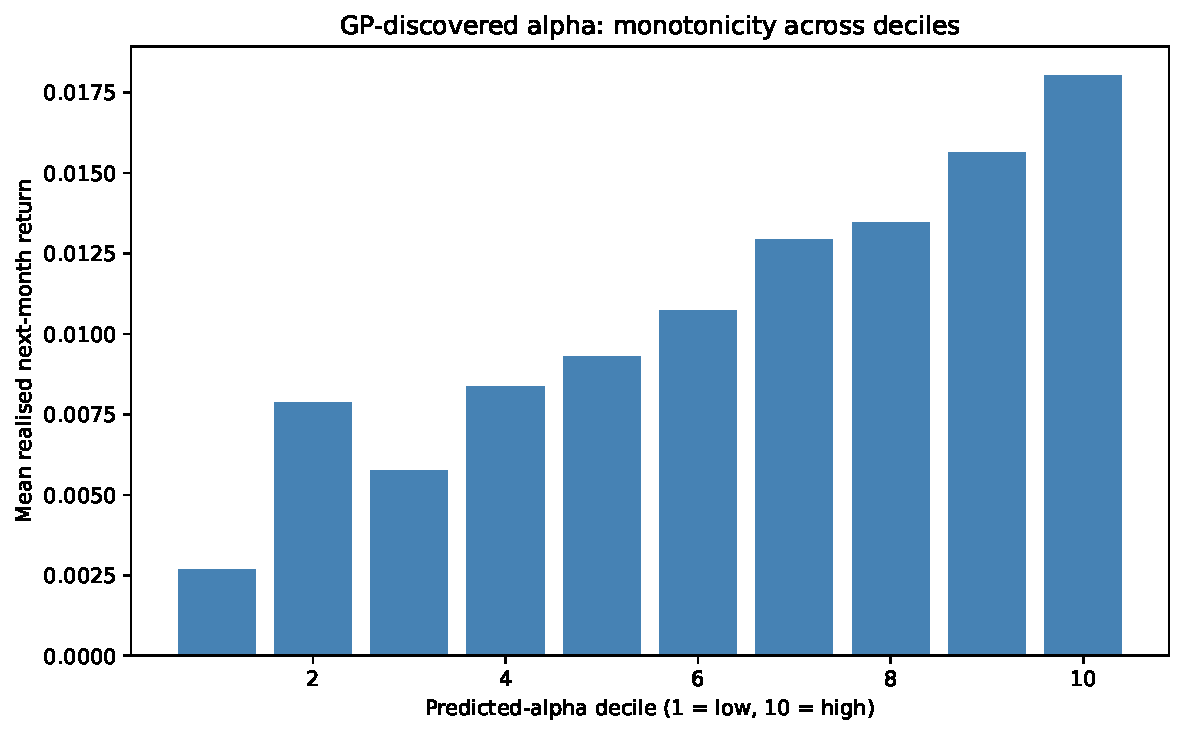
\includegraphics[width=0.7\linewidth]{files/c5ff22851fed0b9afa80c164716a4b4d.pdf}

FIGURE 11.6: Mean realised next-month return across deciles of the GP-discovered alpha, computed over the full 2015 to 2019 cross-section (in-sample). The relationship is close to monotone: stocks in the top decile of the evolved formula outperform those in the bottom decile, consistent with the alpha's pooled IC of 0.045.

As FIGURE 11.6 illustrates, the evolved formula produces a near-monotone spread in realised returns across its deciles. The discovered alpha is economically interpretable: after simplification it rewards low valuation (\texttt{PB}) and penalises volatility (\texttt{vol\_252}) and size (\texttt{size\_log}), a value-and-low-risk tilt of exactly the kind the factor literature documents. Its pooled IC of 0.045 nearly doubles the 0.025 IC of the best single input (\texttt{PB}), showing that GP can combine raw characteristics into a stronger composite than any one of them alone. The magnitude is broadly in line with the out-of-sample IC of 0.047 that \cite{Ren2024} report for warm-started GP on Chinese A-shares, though we stress that our 0.045 is in-sample and would shrink under the walk-forward and multiple-testing corrections of §11.7.1. At production scale, the terminal set would additionally include time-series operators (rank, delay, correlation, ts\_mean, ts\_std) over raw price and volume fields. \cite{Cui2021} formalised this pipeline with AlphaEvolve, a learning framework that combines GP with neural network-based surrogate models to discover novel alphas efficiently. \cite{Yang2024} extended the paradigm by blending GA-generated alpha factors with sentiment features in an ensemble classification framework. \cite{LiQ2024} take a complementary route, feeding GP-discovered symbolic features into an LSTM network to marry the interpretability of formulaic alphas with the sequence-modelling capacity of deep learning. \cite{WangGeng2026} instead make the objective multi-dimensional, evolving factors with a genetic programme whose tri-objective fitness jointly maximises the Sharpe ratio and annualised return while minimising drawdown, re-evolving interpretable factors within a rolling window.

Recent advances have substantially improved the GP alpha mining pipeline:

\begin{itemize}
\item \textbf{Warm Start GP.} \cite{Ren2024} propose initialising the GP population with carefully chosen structural templates rather than random trees. This \textit{warm start} achieves out-of-sample IC of 0.047 (vs. 0.036 for standard GP) and over 50\% annualised returns on Chinese A-shares, demonstrating that domain knowledge injected at initialisation accelerates convergence without sacrificing diversity.
\item \textbf{Alpha-squared.} \cite{Xu2024} reformulate alpha discovery as a program construction task using deep reinforcement learning with a domain-specific language for trading logic. Their approach introduces dimensional analysis for pruning the search space and ensuring logical soundness of discovered alphas. This offers a principled alternative to the purely stochastic search of GP.
\item \textbf{AlphaForge.} \cite{Shi2025} propose a two-stage framework: a generative-predictive neural network mines alpha factors (Stage 1), then dynamically combines them with time-varying weights (Stage 2). This leverages deep learning's spatial exploration capabilities while preserving factor diversity (a key concern when building portfolios from multiple alpha signals).
\item \textbf{Geometric semantic GP.} A recent contribution by \cite{Bunjerdtaweeporn2025} demonstrates that \textit{geometric semantic GP} (in which crossover and mutation operate on the semantics of programs rather than their syntax) provides superior forecast accuracy and portfolio performance for cross-sectional U.S. equity strategies compared to standard GP.
\end{itemize}

These developments suggest that the GP alpha mining field is maturing from a proof-of-concept stage to a production-grade methodology, though the overfitting concerns discussed in §11.7.1 remain paramount.

\textbf{Constrained feature construction.} Between binary feature selection (§11.4.1) and full GP expression trees lies \textbf{constructive induction} \citep{Krawiec2002}: creating new features by applying operators from a finite menu to existing features. In quantitative finance, the operator set typically includes time-series functions (ts\_mean, ts\_std, ts\_delta, ts\_rank, ts\_corr), cross-sectional operators (rank, z-score, winsorize), and arithmetic combinators (ratio, difference, product). A GA chromosome can encode each constructed feature as a fixed-length tuple (operator, operand\_1, operand\_2, lookback\_period) drawn from this menu. This is far simpler than full GP trees, substantially richer than binary masks, and the fixed-length encoding avoids bloat entirely. \cite{Su2022} demonstrate this approach using 206 quantitative factors as building blocks, with Sharpe ratio and factor correlation as fitness criteria. \cite{Xue2016} provide a comprehensive survey of evolutionary approaches to feature selection and construction, documenting how multi-objective formulations (§11.5) can balance predictive power against feature set complexity.

From a practical standpoint, the \texttt{gplearn} library provides an sklearn-compatible implementation of GP-based feature construction via its \texttt{SymbolicTransformer} class. It evolves a population of symbolic expressions, selects the best from a hall-of-fame, and filters to the least correlated set. \cite{Tran2019} show that GP-constructed features can reduce dimensionality to less than 4\% of the original feature set while improving classification performance. For the factor investing setting, this means GP could compress 122 raw characteristics into 5-10 interpretable composite features, each an explicit formula that practitioners can inspect and validate against economic intuition.

\paragraph{Frontiers and extensions}

The three topics below sit at the research frontier of evolutionary methods in quantitative investing. They are less directly tied to the cross-sectional feature-selection problem that anchors this chapter, and we present them without code, but each is an active area where GAs and their descendants are reshaping practice.

\subparagraph{Trading strategy evolution}

Beyond portfolio weights, GAs can evolve entire trading strategies. The chromosome encodes a set of rules (for example, ``buy when the 10-day moving average crosses above the 50-day moving average and RSI is below 30''). This application connects to the seminal work of \cite{Allen1999}, who used GP to discover technical trading rules.

In practice, the rules can be encoded as:

\begin{itemize}
\item \textbf{Threshold-based:} each gene specifies a threshold for a particular indicator (e.g., ``RSI \textless  gene\_1'', ``MACD \textgreater  gene\_2''). The chromosome is a fixed-length real-valued vector where each gene maps to a decision boundary.
\item \textbf{Tree-based (GP):} expression trees combine indicators and logical operators to produce buy/sell signals. Crossover and mutation operate on tree structures rather than vectors.
\item \textbf{Strongly-typed GP (STGP):} a refinement where separate branches handle different data types (e.g., technical indicators versus sentiment scores), enforcing type safety during evolution. \cite{Christodoulaki2025} introduced STGP-SATA, which uses separate tree branches for technical and sentiment analysis, significantly outperforming MLP, SVM, XGBoost, and LSTM benchmarks across Sharpe ratio and risk metrics.
\end{itemize}

We note a critical cautionary point: \cite{Allen1999} found that GP-evolved rules identified favourable market conditions but \textbf{produced no excess returns after realistic transaction costs}. \cite{Neely1997} found slightly more positive results in FX markets. The lesson for practitioners is that trading strategy evolution requires especially careful out-of-sample validation and realistic cost modelling.

More recent contributions have refined the approach. \cite{Salman2022} and \cite{Salman2025} optimise multi-threshold trading strategies under the \textit{directional changes} paradigm, in which price movements are characterised by their magnitude rather than by fixed time intervals. \cite{Long2025} combine this with multi-objective GP and NSGA-II, evolving strategies that simultaneously optimise total return, expected rate of return, and risk. Their approach is tested on 110 stock datasets from 10 international markets. \cite{Menoita2025} introduce \textit{vectorial GP}, in which operations are performed on vectors of indicator values rather than scalar quantities, and show that strongly-typed vectorial GP consistently outperforms standard GP on multi-year financial instrument data.

In the cryptocurrency space, where transaction costs are lower and markets trade continuously, the results have been more encouraging. A recent framework by \cite{Tian2025} integrates GAs with multi-agent coordination for adaptive crypto trading parameter optimisation. On BTC, ETH, and BNB (5-minute frequency, December 2024 to September 2025), the hybrid framework improved total returns by 29\%, 550\%, and 169\% respectively over standard benchmarks, with enhanced Sharpe and Sortino ratios.

Despite these advances, the fundamental warning of \cite{Allen1999} remains relevant: in liquid equity markets with non-trivial transaction costs, evolved trading rules must clear a high bar to deliver net-of-cost profits. The reader should approach this application with the same scepticism that Chapter 14 (§14.4.2) recommends for any backtest.

\subparagraph{Neuroevolution: evolving neural network architectures}

Chapter 8 treated neural networks as fixed architectures whose weights are optimised via gradient descent. A natural question is: can we also optimise the architecture itself? \textbf{Neuroevolution} answers this by using evolutionary algorithms to evolve both the topology and the weights of neural networks. This connects directly to the architectural choices discussed in Chapter 8 (§8.3) (number of layers, neurons, activation functions, connectivity) which are typically made by the user through trial and error or grid search (Chapter 12, §12.3).

Three approaches are particularly relevant for financial applications:

\begin{itemize}
\item \textbf{NEAT} (NeuroEvolution of Augmenting Topologies; \citep{Stanley2002}): starts with minimal networks and progressively adds neurons and connections through structural mutation, using a \textit{speciation} mechanism to protect topological innovations from being eliminated before they mature. \cite{HuangLC2025} applied NEAT to stock trading using seven technical indicators (SMA, KD, MACD, CCI, Williams \%R, RSI, ADOSC) on 22 years of S\&P 500 data (503 stocks, 2000 to 2022). NEAT achieved returns comparable to buy-and-hold but with \textbf{significantly lower risk exposure and greater stability}. This suggests that neuroevolution's value may lie more in risk management than in raw return enhancement.
\item \textbf{EXAMM} (Evolutionary eXploration of Augmenting Memory Models; \citep{Lyu2024}): extends the NEAT paradigm to recurrent architectures, progressively evolving RNNs with LSTM and GRU memory cells. Applied to stock return prediction across all 30 Dow Jones Industrial Average companies, EXAMM-evolved RNNs generated higher returns than the DJI and S\&P 500 indices in both bull (2023) and bear (2022) markets using a simple long-short strategy. \cite{LyuZ2025} subsequently demonstrated that EXAMM-evolved RNNs \textbf{outperform or match transformer-based architectures} across 50 multivariate stock datasets, including a combined dataset with 300 input features and 50 outputs, all while using significantly fewer parameters. This is a striking finding given the current popularity of transformers (see §8.6.4), and it suggests that evolved compact architectures may be better suited to the noisy, non-stationary data typical of financial markets than large pre-trained models.
\item \textbf{GA-optimised neural networks.} A simpler variant uses standard GAs to tune the hyperparameters of a fixed neural network architecture (number of hidden layers, neurons per layer, learning rate, dropout rate, batch size) rather than evolving the topology directly. This approach has been applied successfully to LSTM networks for stock prediction by \cite{Chung2018}, \cite{Chen2021}, \cite{Abraham2022}, and \cite{Zeng2022}, with GAs selecting network depth, hidden units, and learning schedules. \cite{Behera2023} provide a comprehensive survey of evolutionary optimisation for higher-order neural networks in financial forecasting, documenting consistent improvements over manual tuning. \cite{Sutiene2024} confirm in a broader review that evolutionary optimisation of neural architectures remains the dominant paradigm in AI-driven portfolio management.
\end{itemize}

The key advantage of neuroevolution over manual architecture search is automation. The key disadvantage is computational cost: evolving populations of neural networks is expensive. However, the EXAMM results suggest that the evolved architectures are often \textbf{smaller and cheaper to deploy} than hand-designed alternatives, which partially offsets the upfront evolutionary cost.

\subparagraph{LLM-GA hybrids: the frontier of alpha mining}

The most recent development at the intersection of evolutionary computation and quantitative finance is the combination of large language models (LLMs) with genetic algorithms. These hybrid systems leverage the LLM's ability to reason about financial concepts and generate syntactically valid factor expressions, while using evolutionary search to optimise and diversify the factor pool. The pace of publication in this area is remarkable: at the time of writing, over a dozen systems have been proposed within a two-year span. We list the most prominent ones in TABLE 11.5.

TABLE 11.5: LLM-GA and evolutionary hybrid systems for alpha mining (2023 to 2026).

\bigskip\noindent
\begin{tabular}{p{\dimexpr 0.200\linewidth-2\tabcolsep}p{\dimexpr 0.200\linewidth-2\tabcolsep}p{\dimexpr 0.200\linewidth-2\tabcolsep}p{\dimexpr 0.200\linewidth-2\tabcolsep}p{\dimexpr 0.200\linewidth-2\tabcolsep}}
\toprule
System & Year & Key innovation & Venue & Reference \\
\hline
AlphaGen & 2023 & PPO-based RL for synergistic factor discovery & KDD & \cite{Yu2023} \\
Alpha-GPT & 2023 & LLM-assisted alpha mining via prompt engineering & arXiv & \cite{wang2023alphagpt} \\
Alpha-GPT 2.0 & 2024 & Multi-agent LLM: mining, modelling, analysis agents & arXiv & \cite{Yuan2024} \\
AlphaForge & 2025 & Generative NN + dynamic factor combination & AAAI & \cite{Shi2025} \\
AlphaAgent & 2025 & AST-based originality + complexity control vs. alpha decay & KDD & \cite{tang2025alphaagent} \\
Chain-of-Alpha & 2025 & Dual-chain architecture (generation + optimisation) & arXiv & \cite{Cao2025} \\
CogAlpha & 2025 & LLMs as cognitive agents: multi-stage mutation/recombination & arXiv & Liu, F. et al. (2025) \\
ELfolio & 2025 & LLM-driven strategy evolution for portfolio optimisation & Intelligent Computing & Zeng, X. et al. (2025) \\
EFS & 2025 & Evolutionary factor search for sparse portfolio construction & arXiv & \cite{Luo2025} \\
QuantaAlpha & 2026 & Trajectory-level mutation/crossover; cross-market transfer & arXiv & Han, J. et al. (2026) \\
\bottomrule
\end{tabular}

\bigskip

We briefly comment on three systems that illustrate the trajectory of this subfield.

\textbf{AlphaAgent} \citep{tang2025alphaagent} is notable for directly addressing the overfitting problem (the Achilles' heel of evolutionary alpha mining; see §11.7.1). It incorporates three regularisation mechanisms: (i) AST-based (Abstract Syntax Tree) originality enforcement, which prevents the LLM from generating alphas that are syntactically similar to existing ones; (ii) hypothesis-factor semantic alignment, which ensures that generated factors are logically consistent with the financial hypothesis that motivated them; and (iii) complexity control, which penalises over-engineered expressions prone to overfitting. On the CSI 500, AlphaAgent achieved 11.0\% annual excess return with an information ratio of 1.5 after transaction costs. These metrics would be noteworthy if confirmed out-of-sample.

\textbf{Chain-of-Alpha} \citep{Cao2025} replaces the tree-based evolutionary search with a \textit{chain-based reasoning} architecture, consisting of a Factor Generation Chain (which produces candidate alphas) and a Factor Optimisation Chain (which refines them). This dual-chain design achieves full automation (no human intervention is required) and demonstrates strong scalability on A-share benchmarks.

\textbf{ELfolio} \citep{ZengX2025} takes a different approach by evolving entire portfolio \textit{strategies} rather than individual alpha factors. The system uses LLMs to automatically generate and evolve heuristic portfolio strategies across multiple paradigms (RL, evolutionary search, deep learning), selecting and recombining the best-performing approaches. This connects the LLM-GA literature to the ensemble and model combination ideas discussed in Chapter 13.

Two further entries in TABLE 11.5 illustrate the breadth of the paradigm: EFS \citep{Luo2025} casts sparse portfolio construction as an LLM-guided evolutionary factor search, while CogAlpha \citep{LiuF2025} treats the language model as a cognitive agent that mutates and recombines factor code across successive stages.

We emphasise that these systems represent the research frontier, and their real-world performance remains to be validated at scale with proper out-of-sample testing. \cite{ZhangJ2025} identify several open challenges in their survey of LLM-based alpha mining: simplified performance evaluation (most papers use IC or Sharpe alone), limited numerical understanding by LLMs, lack of diversity in generated factors, weak exploration dynamics, temporal data leakage risks, and regulatory compliance concerns. The reader should approach reported results with the same caution that Chapter 14 (§14.4.2) recommends for any backtest.

\subsubsection{Multi-objective optimisation}

\paragraph{Pareto optimality}

In factor investing, the investor faces multiple competing objectives: maximise expected return, minimise variance, minimise turnover, limit drawdowns, and potentially maximise an ESG score. These objectives typically conflict: higher expected returns come with higher risk. A single scalar fitness function requires the user to specify weights for each objective a priori, which is both subjective and constraining.

\textbf{Multi-objective evolutionary algorithms (MOEAs)} avoid this by seeking the entire set of \textit{Pareto-optimal} solutions. A solution $\mathbf{x}$ dominates $\mathbf{y}$ (written $\mathbf{x} \succ \mathbf{y}$) if and only if:

\begin{equation}
f_m(\mathbf{x}) \geq f_m(\mathbf{y}) \quad \forall \, m = 1, \ldots, M, \qquad \text{and} \qquad f_j(\mathbf{x}) > f_j(\mathbf{y}) \quad \text{for at least one } j. \tag{11.6}
\end{equation}

The \textbf{Pareto front} is the set of all non-dominated solutions. The investor can then choose from this set based on their preferences, informed by the trade-offs revealed by the front.

We illustrate with a concrete example. Consider three portfolios: A (expected return 8\%, volatility 12\%), B (expected return 6\%, volatility 15\%), and C (expected return 7\%, volatility 14\%). Portfolio A dominates both B and C because it achieves higher return \textit{and} lower risk. Portfolios B and C are non-dominated with respect to each other: B has lower return but also, in this case, higher risk, so neither is strictly better. The Pareto front consists of all such non-dominated solutions.

The Pareto front generalises the classical \textit{efficient frontier} of \cite{markowitz1952portfolio}. Each point on the front represents a different trade-off that the investor cannot improve upon without sacrificing at least one objective. The advantage of computing the entire front (rather than a single scalarised optimum, as in Equation 11.5) is that the investor can examine the trade-offs and choose \textit{ex post}, based on preferences that may be difficult to quantify a priori. This is arguably the most compelling reason to use evolutionary multi-objective optimisation in portfolio construction.

In practice, the Pareto front contains tens to hundreds of solutions, depending on the population size and the shape of the objective space. With more objectives (return, risk, turnover, drawdown, ESG score), the front becomes a surface or hypersurface, and the proportion of non-dominated solutions grows rapidly. We discuss the algorithmic consequences of this in §11.5.2.

\paragraph{The NSGA-II algorithm}

The most widely used MOEA is NSGA-II (Non-dominated Sorting Genetic Algorithm II; \citep{Deb2002}). It combines two mechanisms that, together, drive the population toward a well-spread Pareto front.

\textbf{Fast non-dominated sorting.} The population of $N$ individuals is partitioned into successive Pareto fronts $F_1, F_2, \ldots, F_r$. Front $F_1$ contains all non-dominated solutions (i.e., no member of $F_1$ is dominated by any other individual in the population). Front $F_2$ contains solutions dominated only by members of $F_1$, and so on. The naive approach of comparing every pair of solutions has complexity $O(MN^2)$, where $M$ is the number of objectives. The algorithm of \cite{Deb2002} achieves the same result by maintaining, for each solution, a domination count and a list of solutions it dominates, enabling efficient front assignment in a single pass through the population.

\textbf{Crowding distance.} Within each front $F_k$, we need a secondary ranking to decide which solutions to keep when truncating the population. NSGA-II uses \textit{crowding distance}, which measures how isolated each solution is in objective space. For a given objective $m$, the solutions in $F_k$ are sorted by $f_m$, and the boundary solutions (those with the smallest and largest $f_m$ values) receive infinite crowding distance. For interior solutions, the contribution from objective $m$ is $(f_m^{i+1} - f_m^{i -1}) / (f_m^{\max} - f_m^{\min})$, where $i+1$ and $i -1$ denote the neighbouring solutions in the sorted order. The total crowding distance is the sum of contributions across all $M$ objectives. Solutions with larger crowding distance occupy less crowded regions of the Pareto front, which promotes diversity and prevents the population from clustering around a few high-fitness points.

\textbf{Selection mechanism.} NSGA-II uses a lexicographic comparison: front rank first (lower is better), then crowding distance (higher is better). A solution on $F_1$ always beats any solution on $F_2$, regardless of crowding distance. Within the same front, the more isolated solution wins. In DEAP, \texttt{tools.selNSGA2} implements this ranking, while \texttt{tools.selTournamentDCD} applies the crowding-distance comparison in a binary tournament context.

\textbf{High-dimensional limitation.} When the number of objectives exceeds approximately three, the proportion of non-dominated solutions in a random population approaches 100\%. This is a combinatorial consequence of high-dimensional dominance: with $M$ objectives, it becomes increasingly unlikely that one solution is better on \textit{all} of them. With nearly all solutions on $F_1$, front-rank comparison loses discriminative power, and selection reduces to crowding distance alone, which itself degrades in high dimensions. This motivates the reference-point mechanism of NSGA-III (§11.5.3).

\cite{Anagnostopoulos2011} comprehensively compared five MOEAs on cardinality-constrained portfolio problems and found NSGA-II and SPEA2 to be generally superior. \cite{Awad2022} further compared NSGA-II and NSGA-III on portfolio management tasks, confirming the advantages of NSGA-III when the number of objectives exceeds three.

\paragraph{NSGA-III}

When the number of objectives exceeds three (for instance, simultaneously maximising return, minimising variance, minimising turnover, limiting drawdown, and maximising an ESG score), NSGA-II's crowding distance mechanism degrades because most solutions become non-dominated in high-dimensional objective spaces. NSGA-III \citep{Deb2014} addresses this by replacing crowding distance with a \textbf{reference-point mechanism}: a set of uniformly distributed reference points in objective space guides the selection process, maintaining diversity even with many objectives.

In a 2025 study, Muteba Mwamba, Mbucici, and Mba \citep{MutebaMwamba2025} applied NSGA-III to portfolio selection and found that it generates more diverse Pareto-optimal portfolios than NSGA-II and MOEA/D, with significantly higher Sharpe ratios, more favourable skewness, and reduced kurtosis. \cite{LarniFooeik2025} integrated ESG performance as a primary objective alongside return and risk in NSGA-III optimisation, filtering 100 stocks from 400 S\&P 500 constituents based on market capitalisation and ESG criteria. This demonstrates that ESG-aware Pareto-optimal portfolio construction is feasible within the evolutionary framework.

\paragraph{Application: return versus risk portfolio}

We apply NSGA-II to find the Pareto front of the bi-objective problem: maximise return, minimise risk. This is the evolutionary analogue of the Markowitz efficient frontier, applied here to the same 30 real US equities used in §11.4.2.

\begin{verbatim}
import numpy as np
import random
from deap import base, creator, tools, algorithms
import matplotlib.pyplot as plt

SEED = 42
np.random.seed(SEED)
random.seed(SEED)

# -- Re -use the real return moments from §11.4.2 -------------
import pandas as pd
data_ml = pd.read_parquet('data/mlfi_us_data.parquet')
data_ml = data_ml.rename(columns={'id': 'stock_id'})
win = data_ml[data_ml['date'].between('2015-01-01', '2019-12-31')]
returns = win.pivot_table(index='date', columns='stock_id',
                          values='R1M_Usd').dropna(axis=1)
liq = win.groupby('stock_id')['adv_252'].mean()
top = liq[returns.columns].sort_values(ascending=False).head(30).index
R = returns[top]
N_ASSETS = 30
mu = R.mean().values                        # Mean monthly returns
Sigma = R.cov().values                      # Return covariance matrix

# -- Multi -objective fitness ----------------------------------
def evaluate_mo(individual):
    """Return (expected_return, -volatility)."""
    w = np.array(individual)
    w = np.maximum(w, 0)
    if w.sum() < 1e-10:
        return (0.0, -1.0)
    w = w / w.sum()
    ret = w @ mu
    vol = np.sqrt(w @ Sigma @ w)
    return (ret, -vol)         # Maximise return, maximise -vol

# -- DEAP setup for NSGA -II -----------------------------------
creator.create("FitMO", base.Fitness, weights=(1.0, 1.0))
creator.create("IndMO", list, fitness=creator.FitMO)

toolbox = base.Toolbox()
toolbox.register("gene", random.random)
toolbox.register("individual", tools.initRepeat,
                 creator.IndMO, toolbox.gene, n=N_ASSETS)
toolbox.register("population", tools.initRepeat,
                 list, toolbox.individual)
toolbox.register("evaluate", evaluate_mo)
toolbox.register("mate", tools.cxBlend, alpha=0.3)
toolbox.register("mutate", tools.mutGaussian,
                 mu=0, sigma=0.1, indpb=0.2)
toolbox.register("select", tools.selNSGA2)

# -- Run NSGA -II ----------------------------------------------
N_POP, N_GEN = 200, 100
pop = toolbox.population(n=N_POP)

# Evaluate initial population
fitnesses = list(map(toolbox.evaluate, pop))
for ind, fit in zip(pop, fitnesses):
    ind.fitness.values = fit
pop = toolbox.select(pop, N_POP)   # assign crowding distance

for gen in range(N_GEN):
    offspring = tools.selTournamentDCD(pop, len(pop))
    offspring = [toolbox.clone(ind) for ind in offspring]
    for c1, c2 in zip(offspring[::2], offspring[1::2]):
        if random.random() < 0.7:
            toolbox.mate(c1, c2)
            del c1.fitness.values, c2.fitness.values
    for mut in offspring:
        if random.random() < 0.2:
            toolbox.mutate(mut)
            del mut.fitness.values
    invalids = [ind for ind in offspring
                if not ind.fitness.valid]
    fitnesses = map(toolbox.evaluate, invalids)
    for ind, fit in zip(invalids, fitnesses):
        ind.fitness.values = fit
    pop = toolbox.select(pop + offspring, N_POP)

# -- Extract Pareto front -------------------------------------
fits = np.array([ind.fitness.values for ind in pop])

# Identify non-dominated solutions
front = tools.sortNondominated(pop, len(pop),
                               first_front_only=True)[0]
front_fits = np.array([ind.fitness.values for ind in front])

# Sort Pareto front by risk for cleaner plot
order = np.argsort(front_fits[:, 1])
front_fits = front_fits[order]

# -- Plot -----------------------------------------------------
fig, ax = plt.subplots(figsize=(8, 6))
ax.scatter(-fits[:, 1], fits[:, 0], alpha=0.3,
           s=10, label="All portfolios")
ax.plot(-front_fits[:, 1], front_fits[:, 0], "r-o",
        markersize=4, label="Pareto front")

# Individual assets
for i in range(N_ASSETS):
    vol_i = np.sqrt(Sigma[i, i])
    ax.scatter(vol_i, mu[i], c="grey", s=30,
               marker="^", zorder=5)

ax.set_xlabel("Volatility")
ax.set_ylabel("Expected Return")
ax.set_title("NSGA-II: Evolved Efficient Frontier")
ax.legend()
plt.tight_layout()
plt.show()
\end{verbatim}

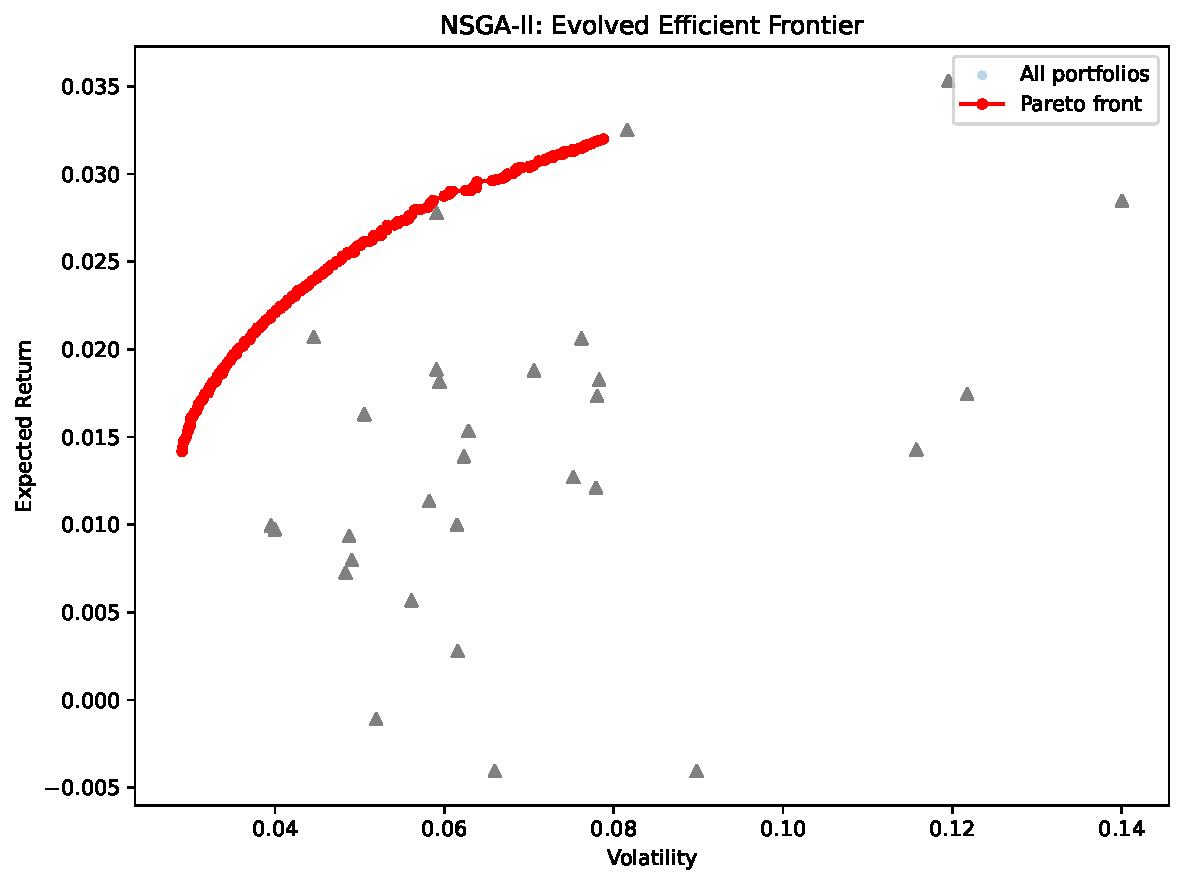
\includegraphics[width=0.7\linewidth]{files/32f5e32ceefeb574ee9f1a32d9426e55.pdf}

FIGURE 11.7: The NSGA-II-evolved Pareto front (red) for 30 real US equities (2015 to 2019), with monthly return and volatility on the axes. Grey triangles represent individual assets. The Pareto front dominates all individual assets: diversified portfolios achieve better return-risk trade-offs. Unlike the classical Markowitz frontier, the GA can handle additional constraints (cardinality, turnover, sector limits) without changing the algorithmic framework.

The Pareto front in FIGURE 11.7, comprising 200 non-dominated portfolios that span monthly returns of roughly 1.4\% to 3.2\%, closely approximates the classical efficient frontier obtained by quadratic programming on these same 30 stocks. The key advantage is generality: the same NSGA-II framework can accommodate additional objectives (turnover, drawdown, ESG) and constraints (cardinality, sector limits) without reformulating the mathematical program.

\subsubsection{Full empirical application}

\paragraph{Setup and data}

We now present a complete empirical application that ties together the concepts from this chapter. The setting mirrors the backtesting framework of Chapter 14 (see Section 14.2 for the general signal-to-weight pipeline): a walk-forward protocol applied to a factor selection problem using the full dataset described in Chapter 5. We then extend the analysis with multi-objective feature selection (§11.6.4) and GA-based hyperparameter tuning (§11.6.5).

The dataset spans January 2002 to March 2026 and contains monthly observations on 1,959 US stocks with 122 candidate features across value, momentum, quality, size, and technical categories. The target variable is the one-month forward return (\texttt{R1M\_Usd}). We compare three approaches to constructing a predictive model:

\begin{enumerate}
\item \textbf{GA-selected features:} the GA chooses an optimised subset at each rebalancing date.
\item \textbf{All features:} the full set of 122 features is used without any selection.
\item \textbf{Short list:} a curated subset of 8 well-known factors: \texttt{size\_log}, \texttt{PB}, \texttt{PE}, \texttt{Div\_yld}, \texttt{mom\_252}, \texttt{ROE}, \texttt{vol\_252}, and \texttt{Debt\_Assets}.
\end{enumerate}

\begin{verbatim}
import numpy as np
import pandas as pd
import random
from deap import base, creator, tools, algorithms

SEED = 42
np.random.seed(SEED)
random.seed(SEED)

data_ml = pd.read_parquet('data/mlfi_us_data.parquet')
data_ml = data_ml.rename(columns={'id': 'stock_id'})
data_ml['date'] = pd.to_datetime(data_ml['date'])
dates = sorted(data_ml['date'].unique())
\end{verbatim}

We define the feature space by excluding only the identifiers and the forward-return target variables, retaining all 122 candidate predictors. We deliberately keep the two Sharpe-adjusted momentum columns (\texttt{Mom\_Sharp\_11M} and \texttt{Mom\_Sharp\_5M}): although each is a ratio of a raw momentum factor to its volatility, and hence partly redundant with predictors already present, we prefer to let the GA decide whether they add value rather than pruning them by hand.

\begin{verbatim}
exclude = ['stock_id', 'date', 'R1M_Usd', 'R3M_Usd', 'R6M_Usd',
           'R12M_Usd']
features = [c for c in data_ml.columns if c not in exclude]
K = len(features)
print(f"Data: {len(data_ml):,} rows, "
      f"{data_ml['stock_id'].nunique():,} stocks, "
      f"{K} features")
\end{verbatim}

\begin{verbatim}
Data: 446,388 rows, 1,959 stocks, 122 features
\end{verbatim}

The 122 features provide a rich but potentially redundant feature space. As discussed in Chapter 6, penalised regressions address this redundancy via shrinkage; here, the GA tackles the same problem through explicit combinatorial selection.

\paragraph{Walk-forward protocol}

The walk-forward (rolling window) protocol mirrors Chapter 14 (§14.1):

\begin{enumerate}
\item At each rebalancing date $t$, use the previous $s = 60$ months as the training window.
\item Compute the average signed IC for each feature over the training window; record the sign (+1 or -1).
\item Run the GA to select features that maximise the signed IC of a sign-corrected composite.
\item Run the GA three times with different seeds and retain features selected by at least two of three runs (majority vote).
\item Fit a Ridge regression on the sign-corrected selected features using recent training data.
\item Compute the out-of-sample Spearman IC at time $t$.
\item Roll forward by one month and repeat.
\end{enumerate}

A subtle but important design choice is the fitness function. A naive implementation might use the absolute value of the IC, reasoning that a feature with IC = -0.05 is ``just as predictive'' as one with IC = +0.05. However, when these features are combined in an equal-weighted composite, their signals can cancel. The sign-aware approach resolves this: we first compute each feature's average IC over the training window, then flip the sign of features with negative average IC before forming the composite. The GA fitness is the signed IC of this corrected signal.

\begin{verbatim}
from scipy.stats import rankdata

def compute_feature_signs(train_date_list):
    """Average signed IC per feature; return +1/-1."""
    ic_matrix = []
    for d in train_date_list:
        dd = date_data[d]
        ics = (dd['X_rank'] * dd['y_rank'][:, None])
        ics = ics.mean(axis=0)               # Vectorised correlation
        ic_matrix.append(ics)
    avg_ic = np.nanmean(ic_matrix, axis=0)
    return np.where(avg_ic >= 0, 1.0, -1.0)
\end{verbatim}

The fitness function uses these signs to build a coherent composite signal. We also add a mild cardinality penalty that discourages subsets larger than 50 features, nudging the GA toward parsimonious solutions.

\begin{verbatim}
def evaluate(individual):
    """Fitness = avg signed IC of sign-corrected composite."""
    sel = np.array(individual, dtype=bool)
    n_sel = sel.sum()
    if n_sel == 0:
        return (0.0,)
    ics = []
    for X_r, y_r in zip(X_ranks, y_ranks):
        signal = (X_r[:, sel] * signs[sel]).mean(axis=1)
        ic = np.corrcoef(signal, y_r)[0, 1]
        if not np.isnan(ic):
            ics.append(ic)                    # Signed, not abs()
    if not ics:
        return (0.0,)
    mean_ic = np.mean(ics)
    if n_sel > 50:                            # Cardinality penalty
        mean_ic -= 0.001 * (n_sel - 50)
    return (mean_ic,)
\end{verbatim}

The variables \texttt{X\_ranks} and \texttt{y\_ranks} contain pre-computed rank-normalised cross-sections for each training month. Rank-normalising before the GA loop avoids redundant computation across the thousands of fitness evaluations.

To reduce sensitivity to random initialisation, we run the GA three times with different seeds and retain features selected by at least two of three runs (majority vote). This ensemble approach stabilises the selection at modest additional cost.

\begin{verbatim}
ENSEMBLE_SEEDS = 3

def ensemble_ga(train_date_list, base_seed=42):
    """Majority-vote consensus across multiple GA seeds."""
    all_masks = []
    for i in range(ENSEMBLE_SEEDS):
        mask, _ = ga_select_factors(
            train_date_list, seed=base_seed + i * 1000)
        all_masks.append(mask.astype(int))
    vote = np.sum(all_masks, axis=0)
    return vote >= 2                          # At least 2 of 3
\end{verbatim}

The DEAP toolbox is configured identically to the examples in Section 11.3: binary encoding, uniform crossover, bit-flip mutation with per-gene probability $1/K \approx 0.008$, and tournament selection with size 3.

\begin{verbatim}
creator.create("FitnessMax", base.Fitness, weights=(1.0,))
creator.create("Individual", list,
               fitness=creator.FitnessMax)
POP_SIZE = 40
N_GEN = 25
P_CROSS = 0.8
P_MUT = 1.0 / K
\end{verbatim}

The walk-forward loop iterates over 98 out-of-sample months from January 2018 to February 2026. For each month, the ensemble GA selects features on the 60-month training window. A Ridge regression is then fitted on the sign-corrected selected features using the most recent 12 months of training data, and we compute the out-of-sample Spearman IC.

\begin{verbatim}
from sklearn.linear_model import Ridge
from scipy.stats import spearmanr

separation_date = pd.Timestamp('2018-01-31')
TRAIN_WINDOW = 60
\end{verbatim}

The inner loop runs the ensemble GA at each rebalancing date, fits a Ridge regression on the sign-corrected features, and records the out-of-sample IC. The sign correction is applied to both training and test features, ensuring that Ridge receives consistently oriented inputs. The helper functions \texttt{get\_train\_dates}, \texttt{pool\_recent}, and \texttt{get\_cross\_section} handle date indexing and data retrieval; the full implementation is available in the companion repository.

\begin{verbatim}
for test_date in test_dates:
    train_list = get_train_dates(test_date, TRAIN_WINDOW)
    signs = compute_feature_signs(train_list)
    mask_ga = ensemble_ga(train_list)
    feature_freq += mask_ga

    X_pool, y_pool = pool_recent(train_list[-12:])
    X_test, y_test = get_cross_section(test_date)

    # Sign-correct before Ridge
    X_tr = X_pool[:, mask_ga] * signs[mask_ga]
    X_te = X_test[:, mask_ga] * signs[mask_ga]
    reg = Ridge(alpha=1.0).fit(X_tr, y_pool)
    ic_ga, _ = spearmanr(reg.predict(X_te), y_test)
    oos_ics_ga.append(ic_ga)
\end{verbatim}

\paragraph{Results and discussion}

\begin{verbatim}
print(f"{'Method':<25} {'Mean IC':>8} {'Std IC':>8} "
      f"{'IC>0':>8} {'IR':>8}")
print("-" * 55)
for name, arr in [('GA selection', oos_ics_ga),
                  ('All features (122)', oos_ics_all),
                  ('Short list (8)', oos_ics_short)]:
    ir = arr.mean() / arr.std()
    print(f"{name:<25} {arr.mean():>8.4f} "
          f"{arr.std():>8.4f} {(arr > 0).mean():>8.1%}"
          f" {ir:>8.3f}")
print(f"\nAvg factors selected: "
      f"{np.mean(n_sel):.1f} / {K}")
\end{verbatim}

\begin{verbatim}
Method                   Mean IC  Std IC    IC>0       IR
-------------------------------------------------------
GA selection              0.0069  0.1275   52.0%    0.054
All features (122)        0.0046  0.1142   56.1%    0.040
Short list (8)            0.0159  0.1643   52.0%    0.097

Avg factors selected: 38.4 / 122
\end{verbatim}

The results tell a nuanced story. The GA-selected subset achieves a mean out-of-sample IC of 0.007, roughly 50\% higher than the kitchen-sink model using all 122 features (0.005), while retaining only about a third of them. The information ratio (mean IC divided by its standard deviation) improves from 0.040 (all features) to 0.054 (GA selection). The GA thus delivers measurable dimensionality reduction, eliminating approximately 84 features that contribute mainly noise. The positive hit rate of 52\% indicates a slight but consistent edge in the direction of prediction.

However, the curated short list of 8 features achieves the highest mean IC (0.016) and information ratio (0.097) despite using only 7\% of the feature space. This is a humbling result for automated selection, and it highlights a recurring theme in factor investing (see also Chapter 6): expert knowledge, distilled into a small set of well-understood factors, can be difficult to beat with purely data-driven methods. The short list's higher volatility (standard deviation 0.164 vs. 0.128 for the GA) reflects its concentration in fewer features, which amplifies both signal and noise.

\begin{verbatim}
import matplotlib.pyplot as plt

fig, axes = plt.subplots(1, 2, figsize=(14, 5))
cum_ga = np.cumsum(oos_ics_ga)
cum_all = np.cumsum(oos_ics_all)
cum_short = np.cumsum(oos_ics_short)
axes[0].plot(dates_oos, cum_ga,
             label='GA selection (38 features)',
             linewidth=2, color='steelblue')
axes[0].plot(dates_oos, cum_all,
             label='All features (122)',
             linewidth=1.5, linestyle='--', color='coral')
axes[0].plot(dates_oos, cum_short,
             label='Short list (8)',
             linewidth=1.5, linestyle=':', color='forestgreen')
axes[0].set_xlabel('Date')
axes[0].set_ylabel('Cumulative IC')
axes[0].legend()
\end{verbatim}

\begin{verbatim}
axes[1].hist(oos_ics_ga, bins=25, alpha=0.5,
             label='GA selection', color='steelblue')
axes[1].hist(oos_ics_all, bins=25, alpha=0.5,
             label='All features', color='coral')
axes[1].set_xlabel('Monthly IC')
axes[1].set_ylabel('Frequency')
axes[1].legend()
plt.tight_layout()
plt.show()
\end{verbatim}

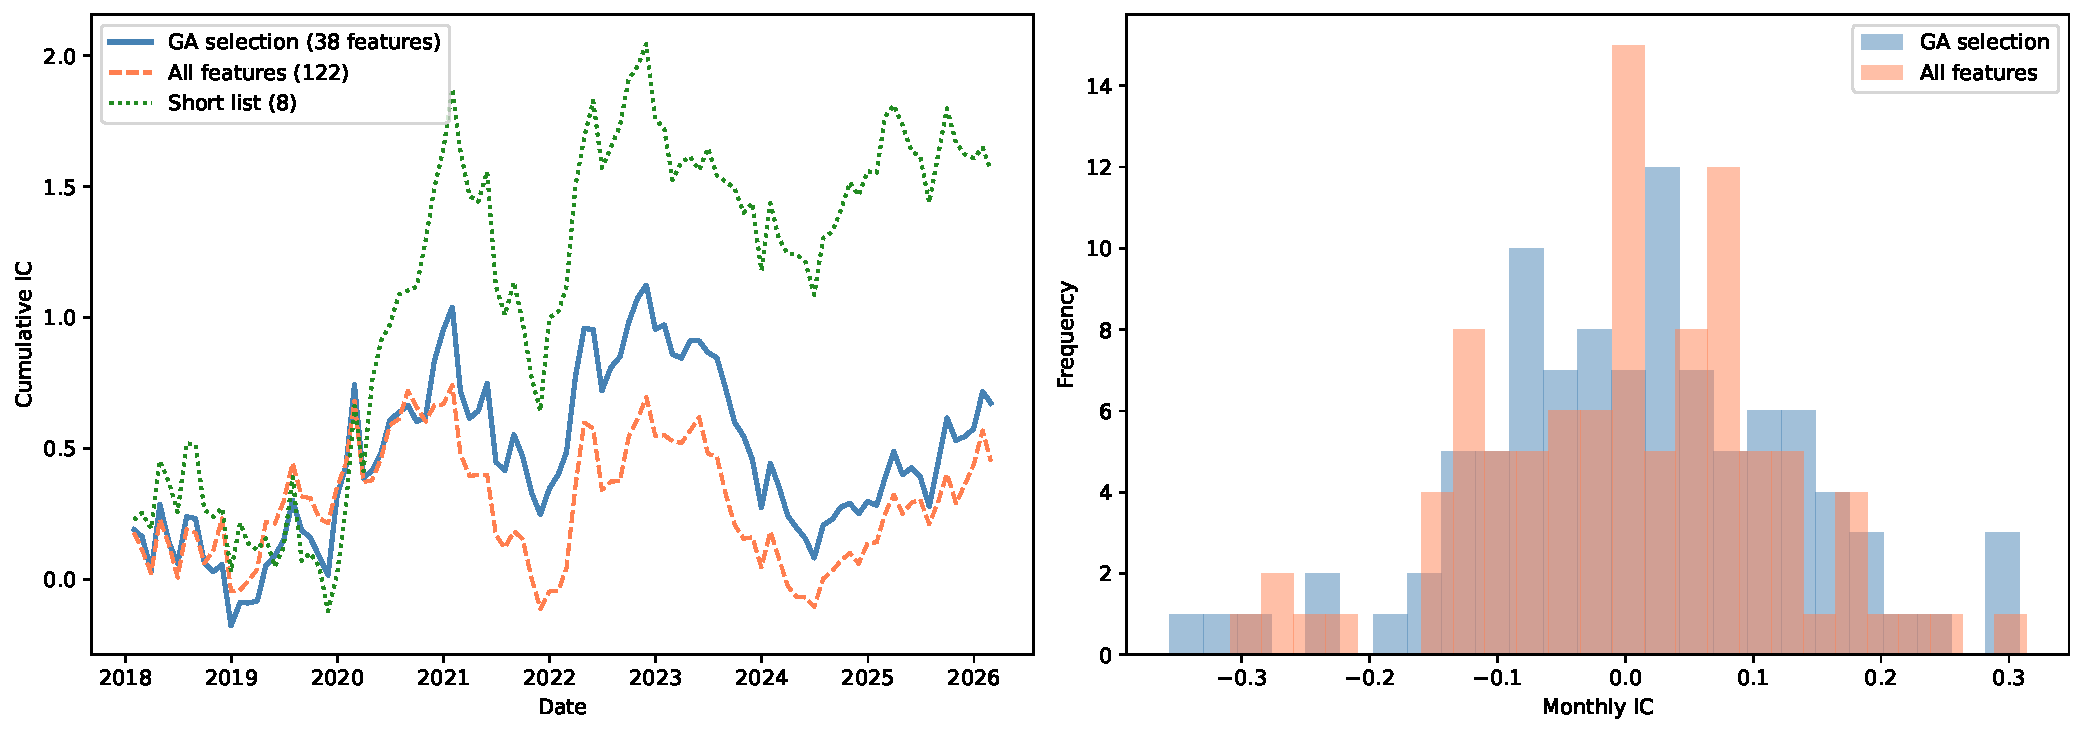
\includegraphics[width=0.7\linewidth]{files/dddecea5c55e51cbdaa6fec317ac73da.pdf}

FIGURE 11.8: \textbf{Left:} Cumulative out-of-sample IC over the walk-forward period (January 2018 to February 2026). The GA-selected model (blue, solid) consistently outpaces the all-features baseline (coral, dashed). The curated short list (green, dotted) achieves the highest cumulative IC, albeit with greater volatility. \textbf{Right:} Distribution of monthly ICs for the GA and all-features approaches. Both distributions are centred near zero with heavy tails, characteristic of cross-sectional return prediction.

As illustrated in FIGURE 11.8, the GA-selected model accumulates IC steadily above the all-features baseline over the eight-year evaluation period. The short list leads overall but exhibits wider swings, consistent with its higher IC standard deviation. The COVID-19 market dislocation in early 2020 produces a sharp negative spike across all three methods, underscoring the difficulty of cross-sectional prediction during regime changes.

The feature selection frequency across the 98 walk-forward windows reveals which factors the GA persistently values.

\begin{verbatim}
freq_df = pd.DataFrame({
    'feature': features,
    'frequency': feature_freq / len(test_dates)
}).sort_values('frequency', ascending=False)

fig, ax = plt.subplots(figsize=(10, 7))
top = freq_df.head(25)
ax.barh(range(25), top['frequency'] * 100,
        color='steelblue', alpha=0.8)
ax.set_yticks(range(25))
ax.set_yticklabels(top['feature'])
ax.invert_yaxis()
ax.set_xlabel('Selection frequency (%)')
plt.tight_layout()
plt.show()
\end{verbatim}

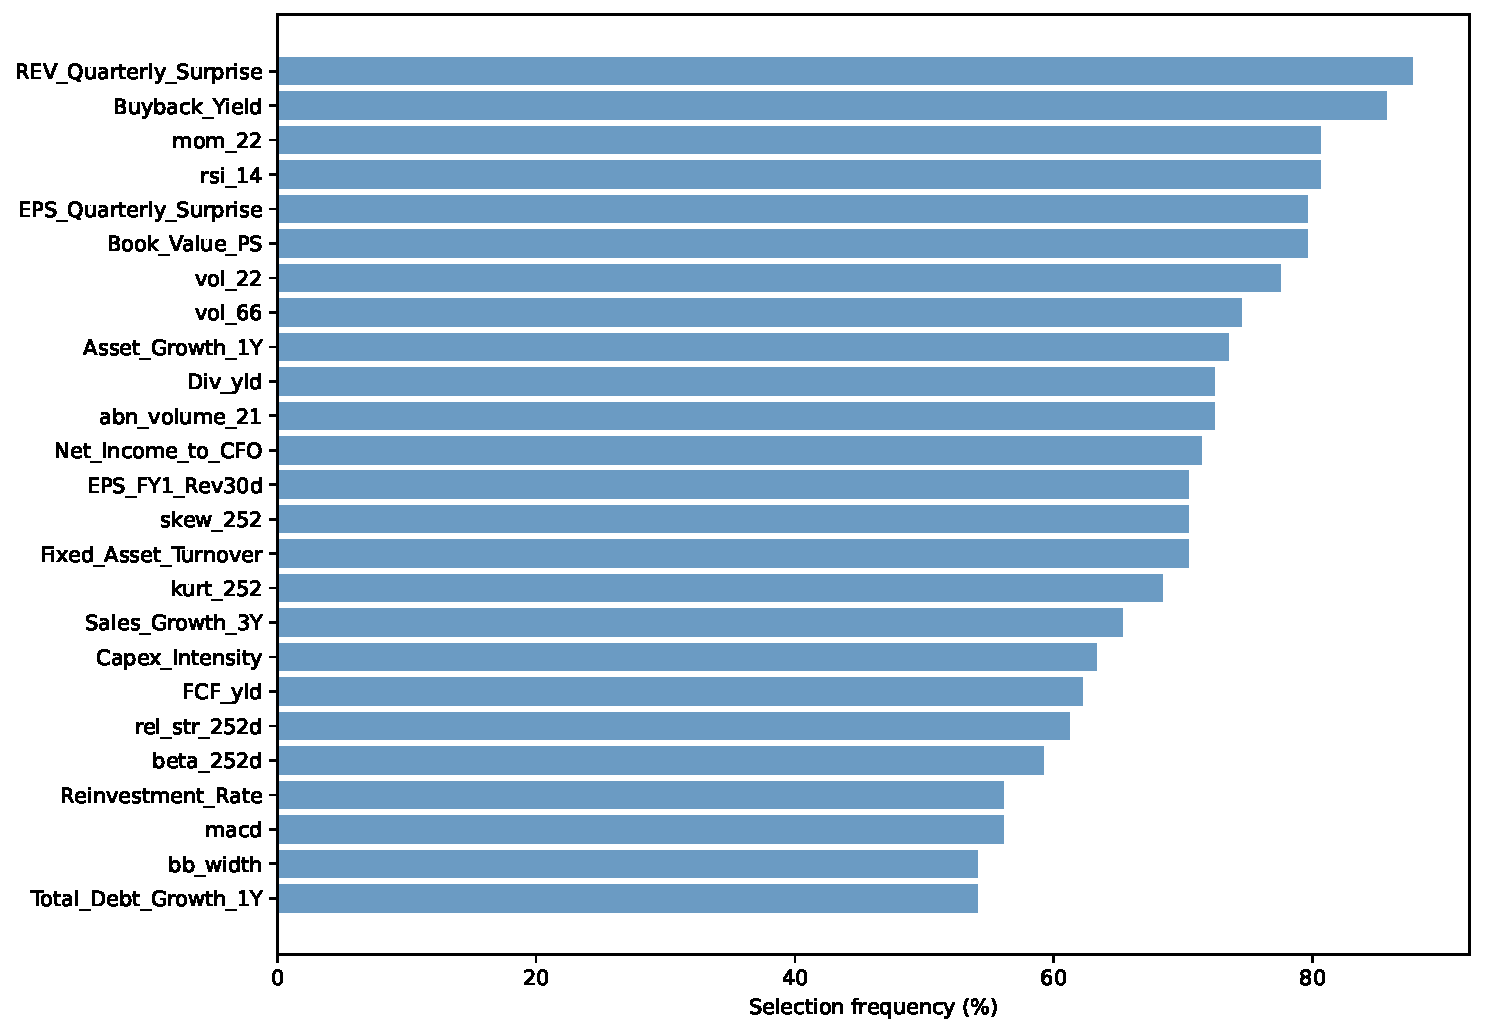
\includegraphics[width=0.7\linewidth]{files/a9138a3843accc600d5e46517fc85473.pdf}

FIGURE 11.9: Selection frequency of the 25 most frequently chosen features across 98 walk-forward windows. Earnings surprise (\texttt{REV\_Quarterly\_Surprise}, 88\%), buyback yield (\texttt{Buyback\_Yield}, 86\%), and short-term momentum (\texttt{mom\_22}, 81\%) are selected most frequently. The top 25 features span momentum, value, earnings, and volatility categories, reflecting a diversified selection profile.

The frequency analysis in FIGURE 11.9 yields several insights. First, the GA selects a diversified mix of factor categories: momentum signals (\texttt{mom\_22}, \texttt{rsi\_14}, \texttt{rel\_str\_252d}), earnings surprise factors (\texttt{REV\_Quarterly\_Surprise}, \texttt{EPS\_Quarterly\_Surprise}, \texttt{EPS\_FY1\_Rev30d}), and volatility measures (\texttt{vol\_22}, \texttt{vol\_66}, \texttt{skew\_252}) all appear in the top 25. Second, the selection is notably more diversified than one might expect: even the most frequent feature (\texttt{REV\_Quarterly\_Surprise}) is chosen in only 88\% of windows, and no feature is selected universally, indicating that the ensemble voting mechanism prevents over-reliance on any individual predictor. Third, several features from the curated short list (e.g., \texttt{Div\_yld} at 72\%) are selected frequently but not universally, suggesting the GA values them as part of a larger ensemble rather than as standalone signals.

The GA selects approximately 38 features on average (31\% of the feature space), a substantial reduction that improves the signal-to-noise ratio without discarding information entirely. This intermediate approach sits between the aggressive shrinkage of L1 penalisation (Chapter 6), which tends to select fewer features, and the implicit feature weighting of ensemble methods (Chapter 7), which use all features but weight them unequally.

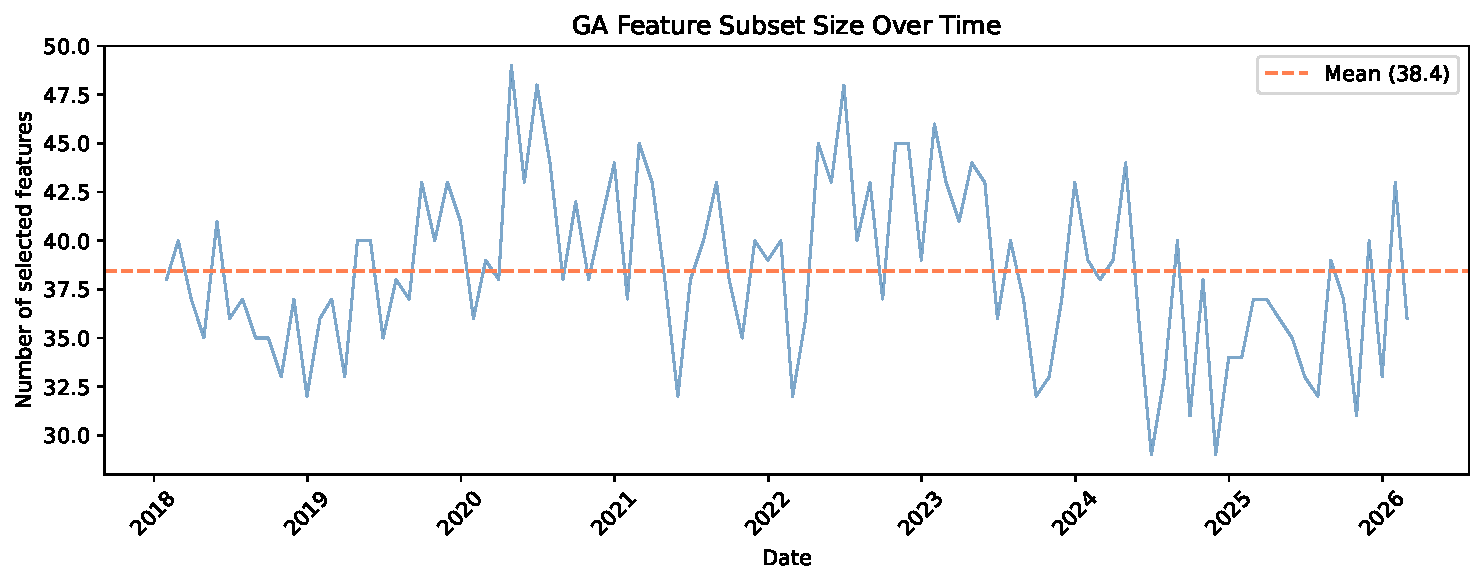
\includegraphics[width=0.7\linewidth]{files/bff9b15100cca9ea303a74d06f4d1526.pdf}

FIGURE 11.10: Number of features selected by the GA at each walk-forward window. The mean is approximately 38 features (dashed line), with moderate variation across time. The cardinality penalty keeps subsets below 50 features in most windows.

FIGURE 11.10 plots the number of selected features at each walk-forward window, showing that the count fluctuates moderately around this 38-feature mean while the cardinality penalty holds most windows below 50. The result echoes a broader lesson: \textbf{more features are not always better}, and the GA provides a principled, adaptive mechanism for navigating the feature space. However, the gap between the GA and the curated short list suggests that, at least in this setting, decades of academic research on factor investing have produced a small set of features that is remarkably hard to improve upon with automated search alone.

\paragraph{Multi-objective feature selection}

The trade-off between predictive power (more features) and parsimony (fewer features) need not be resolved by an ad hoc cardinality penalty. Instead, we can treat feature selection as a bi-objective problem and use NSGA-II (§11.5.2) to recover the full Pareto front.

We define two objectives: (1) maximise the mean signed IC of the sign-corrected composite over the training window, and (2) minimise the number of selected features. The encoding and operators are identical to §11.6.2, but the fitness now returns a tuple of two values.

\begin{verbatim}
creator.create("FitnessMO", base.Fitness,
               weights=(1.0, -1.0))
creator.create("IndMO", list,
               fitness=creator.FitnessMO)

def evaluate_mo(individual):
    sel = np.array(individual, dtype=bool)
    n_sel = sel.sum()
    if n_sel == 0:
        return (0.0, K)        # Worst: zero IC, max features
    ics = []
    for X_r, y_r in zip(X_ranks, y_ranks):
        signal = (X_r[:, sel] * signs[sel]).mean(axis=1)
        ic = np.corrcoef(signal, y_r)[0, 1]
        if not np.isnan(ic):
            ics.append(ic)
    return (np.mean(ics) if ics else 0.0, n_sel)
\end{verbatim}

We run NSGA-II with a population of 100 for 60 generations on the last 60 months of training data (January 2013 to December 2017).

\begin{verbatim}
POP_MO = 100
N_GEN_MO = 60

tb_mo = base.Toolbox()
tb_mo.register("evaluate", evaluate_mo)
tb_mo.register("select", tools.selNSGA2)
# (other operators as before)

# Run NSGA-II loop ...
\end{verbatim}

\begin{verbatim}
Pareto front: 95 solutions
IC range: [0.045, 0.072]
Features range: [3, 28]

Reference: short list IC = 0.032 (8 features)
Reference: all features IC = 0.042 (122 features)

Selected Pareto-optimal solutions:
  N features     IC
  5            0.056
  10           0.066
  19           0.071
  28           0.072
\end{verbatim}

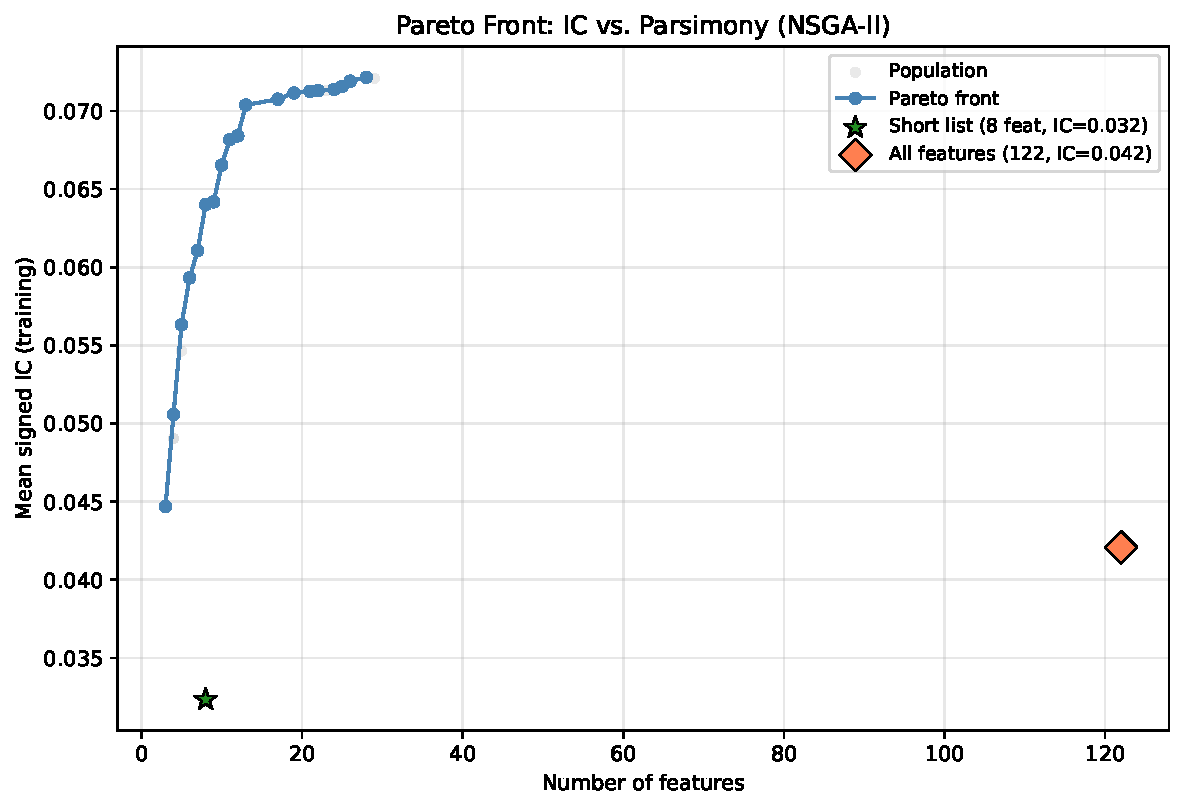
\includegraphics[width=0.7\linewidth]{files/ada8a6aaaa44728fedcebc0336a4244a.pdf}

FIGURE 11.11: Pareto front of the bi-objective feature selection problem (IC vs. number of features). The blue connected line shows the Pareto-optimal trade-off. The green star marks the curated short list (8 features, IC = 0.032) and the coral diamond marks the all-features baseline (122 features, IC = 0.042). The Pareto front dominates both reference points: a 5-feature Pareto solution achieves IC = 0.056, nearly twice the short list's in-sample IC, and a 10-feature solution reaches IC = 0.066.

One caveat frames everything that follows: the ICs in this section are computed in-sample, on the training window itself, and are therefore not directly comparable to the out-of-sample walk-forward figures of §11.6.3, which are roughly an order of magnitude smaller. The aim here is to expose the shape of the IC-versus-parsimony trade-off, not to estimate deployable performance. The gap is real and instructive: the same all-features composite that scores an in-sample IC of 0.042 here delivers an out-of-sample IC of only about 0.005 under the walk-forward protocol of §11.6.3, a collapse that is precisely the overfitting phenomenon dissected in §11.7.1.

FIGURE 11.11 reveals a striking pattern. The Pareto front exhibits strong diminishing returns: the first 5 features capture most of the available IC (0.056 out of a maximum 0.072), while adding features beyond 15 provides negligible improvement. This ``elbow'' in the trade-off curve suggests that the effective dimensionality of the predictive signal is quite low, consistent with the factor investing literature's emphasis on a small number of persistent anomalies \citep{harvey2016and}.

Perhaps most telling is the position of the reference points. The curated short list of 8 features (green star) achieves IC = 0.032, well below the Pareto front at the same feature count, where the NSGA-II solution reaches approximately 0.060. This gap illustrates the value of data-driven selection: the short list's features were chosen for economic interpretability rather than in-sample predictive power, and the NSGA-II solutions exploit signal combinations that domain expertise alone would not identify. Of course, in-sample dominance does not guarantee out-of-sample superiority (§11.7.1), but the Pareto front provides a principled starting point for further investigation.

\paragraph{GA-tuned gradient boosting}

In §11.4.3 we discussed using GAs to tune model hyperparameters. We now demonstrate this on a concrete example: optimising \texttt{GradientBoostingRegressor} from scikit-learn on the 8 short-list features, over a 60-month training window and a 36-month test period (January 2018 to December 2020). Hyperparameter search is precisely where a GA is most dangerous on financial data. As we detail in §11.7.1, an optimiser that maximises an in-sample score will, at the signal-to-noise ratio of monthly cross-sectional returns, reliably find configurations that fit noise. The outcome therefore hinges entirely on the fitness function, not on the GA. We first present a design that makes the GA generalise, then contrast it with the naive alternative.

Three ingredients, each drawn from the financial machine-learning literature, turn the search from a noise-fitting exercise into a disciplined one. First, we bias the search space toward regularisation, since shallow, slow-learning, subsampled trees are the appropriate profile for a high-noise target. We add \texttt{min\_samples\_leaf} as a sixth, strongly regularising gene.

\begin{verbatim}
from sklearn.ensemble import GradientBoostingRegressor

# Regularisation-biased genes: [n_estimators, max_depth, learning_rate,
#                               subsample, max_features, min_samples_leaf]
BOUNDS = [(80, 400), (2, 4), (0.02, 0.15),
          (0.5, 1.0), (0.4, 1.0), (1, 250)]
\end{verbatim}

Second, and most important, we align the fitness with out-of-sample performance instead of interior cross-validation. We score each candidate on the two most recent 12-month blocks of the training window (2016 and 2017), the closest available proxy for the immediately following test period, purging a one-month embargo before each validation block to remove look-ahead leakage \citep{Arian2024}.

\begin{verbatim}
# Validate on the two most recent training years, nearest the test period.
folds = [(train_dates[:-25], train_dates[-24:-12]),   # embargo + 2016 block
         (train_dates[:-13], train_dates[-12:])]       # embargo + 2017 block

def fitness(hp):                                        # recency-aligned, stability-penalised
    ic = []
    for tr, val in folds:
        m = GradientBoostingRegressor(**hp, random_state=SEED).fit(*pool(tr))
        ic.append(np.mean([spearmanr(m.predict(date_data[d]['X']),
                                     date_data[d]['y']).correlation for d in val]))
    ic = np.array(ic)
    return ic.mean() - 0.1 * ic.std()                   # reward stable generalisers
\end{verbatim}

Third, we warm-start the initial population with the default configuration (the §11.6.6 idea applied to hyperparameters) and take the \textit{ensemble} of the eight best configurations rather than a single winner, bagging each over three seeds to trim variance.

\begin{verbatim}
# GA-tuned model = bag the top-8 evolved configurations over three seeds each.
ga_models = [GradientBoostingRegressor(**decode(ind), random_state=s).fit(X_tr, y_tr)
             for ind in hof for s in (42, 7, 123)]
pred = np.mean([m.predict(X_test) for m in ga_models], axis=0)   # ensemble prediction
\end{verbatim}

We run a GA with population 24 for 15 generations, using BLX-$\alpha$ crossover (§11.3.4) and Gaussian mutation, both with bounds clamping. The best recency-validated fitness settles quickly on a conservative configuration.

\begin{verbatim}
GA HP tuning completed in 21 min

Best configuration in the top -8 ensemble:
  n_estimators:      207
  max_depth:         2
  learning_rate:     0.028
  subsample:         0.638
  max_features:      0.925
  min_samples_leaf:  175

Best out -of -sample IC: GA -tuned ensemble (0.052)
\end{verbatim}

We report the evolved configuration against the default and a Ridge benchmark, together with their out-of-sample information coefficients, in TABLE 11.6.

TABLE 11.6: Generalisation-aware GA-tuned gradient boosting versus the default GBR and Ridge: hyperparameters and out-of-sample performance (36 test months, January 2018 to December 2020).

\bigskip\noindent
\begin{tabular}{p{\dimexpr 0.333\linewidth-2\tabcolsep}p{\dimexpr 0.333\linewidth-2\tabcolsep}p{\dimexpr 0.333\linewidth-2\tabcolsep}}
\toprule
Hyperparameter & GA-tuned & Default \\
\hline
n\_estimators & 207 & 100 \\
max\_depth & 2 & 3 \\
learning\_rate & 0.028 & 0.100 \\
subsample & 0.638 & 1.000 \\
max\_features & 0.925 & 1.000 \\
min\_samples\_leaf & 175 & 1 \\
\bottomrule
\end{tabular}

\bigskip

\bigskip\noindent
\begin{tabular}{p{\dimexpr 0.200\linewidth-2\tabcolsep}p{\dimexpr 0.200\linewidth-2\tabcolsep}p{\dimexpr 0.200\linewidth-2\tabcolsep}p{\dimexpr 0.200\linewidth-2\tabcolsep}p{\dimexpr 0.200\linewidth-2\tabcolsep}}
\toprule
Method & Mean IC & Std IC & IC \textgreater  0 & IR \\
\hline
GA-tuned GBR (ensemble) & 0.0524 & 0.087 & 80.6\% & 0.604 \\
Default GBR & 0.0520 & 0.092 & 72.2\% & 0.566 \\
Ridge & 0.0455 & 0.156 & 63.9\% & 0.291 \\
\bottomrule
\end{tabular}

\bigskip

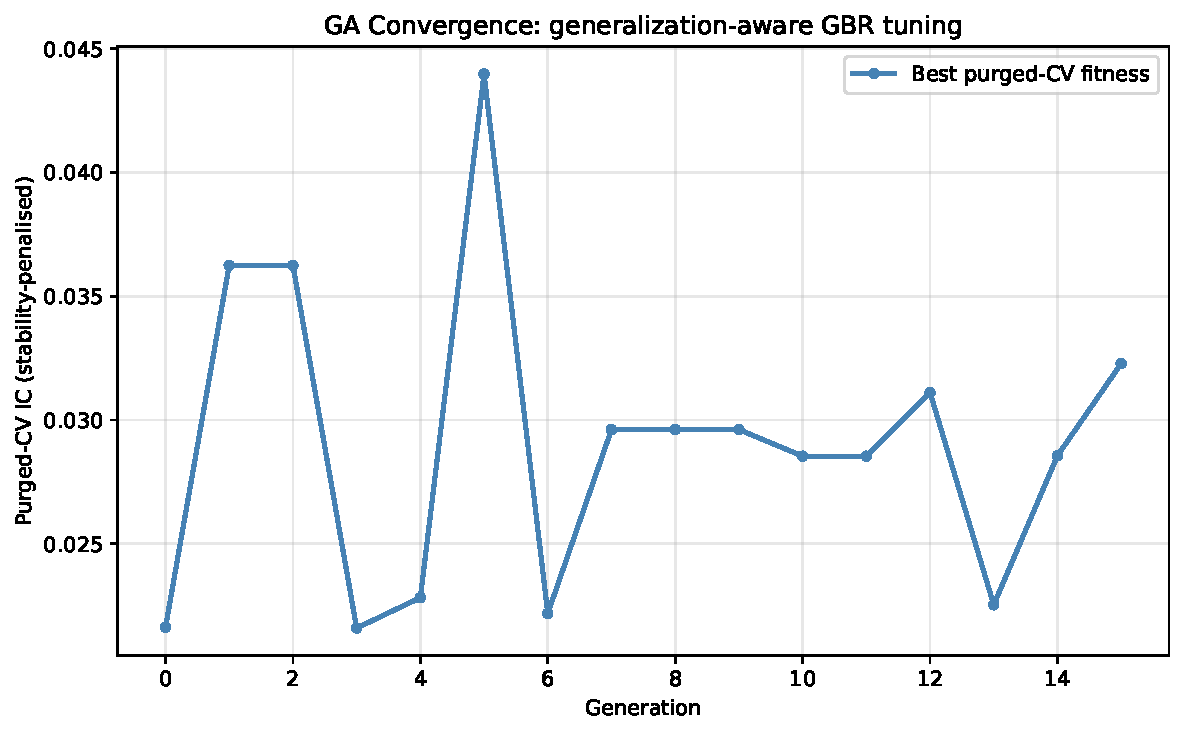
\includegraphics[width=0.7\linewidth]{files/5fe68a41a308474a4b12def608e79a46.pdf}

FIGURE 11.12: GA convergence for generalisation-aware gradient boosting tuning. The best recency-validated fitness (blue) improves over the first several generations and then plateaus. Because the search space and the fitness both favour regularisation, the population settles on shallow, slow-learning configurations rather than the aggressive ones an in-sample fitness would reward.

FIGURE 11.12 traces the GA's convergence toward this regularised region of the search space. The generalisation-aware GA-tuned ensemble delivers the best out-of-sample IC (0.0524), narrowly ahead of the untuned default (0.0520) and well ahead of Ridge (0.0455), and it dominates on every risk-adjusted measure: the highest information ratio (0.60 versus 0.57 and 0.29), the highest hit rate (positive IC in 80.6\% of months, versus 72.2\% and 63.9\%), and the lowest volatility of monthly IC. The evolved configuration is deliberately conservative, with shallow trees (depth 2), a small learning rate (0.028), row subsampling (0.64), and a large minimum leaf size (175 observations), the textbook profile of a regularised learner for a high-noise target.

The contrast with a naive design is the real lesson, and it ties directly to §11.7.1. Had we scored fitness with ordinary in-sample cross-validation over an unconstrained search space (deep trees, large learning rates), the GA would have reproduced the classic failure: it maximises the validation IC yet selects a configuration that overfits, delivering an out-of-sample IC near 0.007, below both baselines. Nothing about the GA changed between the two outcomes; only the fitness function did. Two design choices account for the difference. The search space is biased toward regularisation, so even the fittest individuals are shallow, slow, and subsampled. More importantly, the fitness is aligned with out-of-sample performance: rather than validating on interior folds, we score each candidate on the two most recent training years, the closest legitimate proxy for the immediately following test period, with a one-month embargo to purge look-ahead leakage \citep{Arian2024}. Bagging the top eight configurations then trims the residual variance.

The practical lesson generalises well beyond this example. A GA is only as good as the fitness function it optimises: point it at an in-sample score and it will find noise; point it at a faithful out-of-sample proxy and bias it toward regularisation, and the same algorithm becomes a disciplined search that beats a hand-tuned default. GA hyperparameter tuning is therefore most valuable when the search space contains configurations that are hard to reach by hand (mixed-integer spaces, many interacting parameters) and, above all, when the fitness is a reliable proxy for out-of-sample performance.

\paragraph{Reproducing three recent results}

We close the empirical section by testing three specific claims from the recent literature (§11.4) directly on the book data, applying the same walk-forward discipline used above. Each reproduction is deliberately simple: the aim is to see whether a published finding survives contact with our US equity panel, not to replicate every implementation detail.

\textbf{Warm-start versus cold-start GP \citep{Ren2024}.} \cite{Ren2024} report that seeding the initial GP population with structured factor templates, rather than random trees, improves out-of-sample performance. We test this with an expanding-window walk-forward: at the start of each year from 2011 to 2025 we mine a formulaic alpha on all prior history (§11.4.4) and score its IC on the following twelve months. The warm-start population is seeded (roughly 20\%) with economically motivated templates; the cold-start population is entirely random.

\begin{verbatim}
# Warm start: inject factor templates into the initial GP population
templates = ["mom_252", "rel_str_252d", "ROE", "subtract(mom_252, vol_252)",
             "subtract(Div_yld, vol_252)", "subtract(mom_252, PB)",
             "multiply(ROE, mom_252)", "add(mom_252, rel_str_252d)"]
pop = toolbox.population(n=120)
seeds = [creator.Tree(gp.PrimitiveTree.from_string(templates[i % len(templates)], pset))
         for i in range(len(pop) // 5)]      # ~20% seeded, remainder random
pop[:len(seeds)] = seeds
\end{verbatim}

\begin{verbatim}
Warm start: mean OOS IC = +0.013, hit-rate 73%, IR 0.49
Cold start: mean OOS IC = -0.006, hit-rate 33%, IR -0.23
Warm beats cold in 67% of the 15 yearly test periods (+0.019 mean IC)
\end{verbatim}

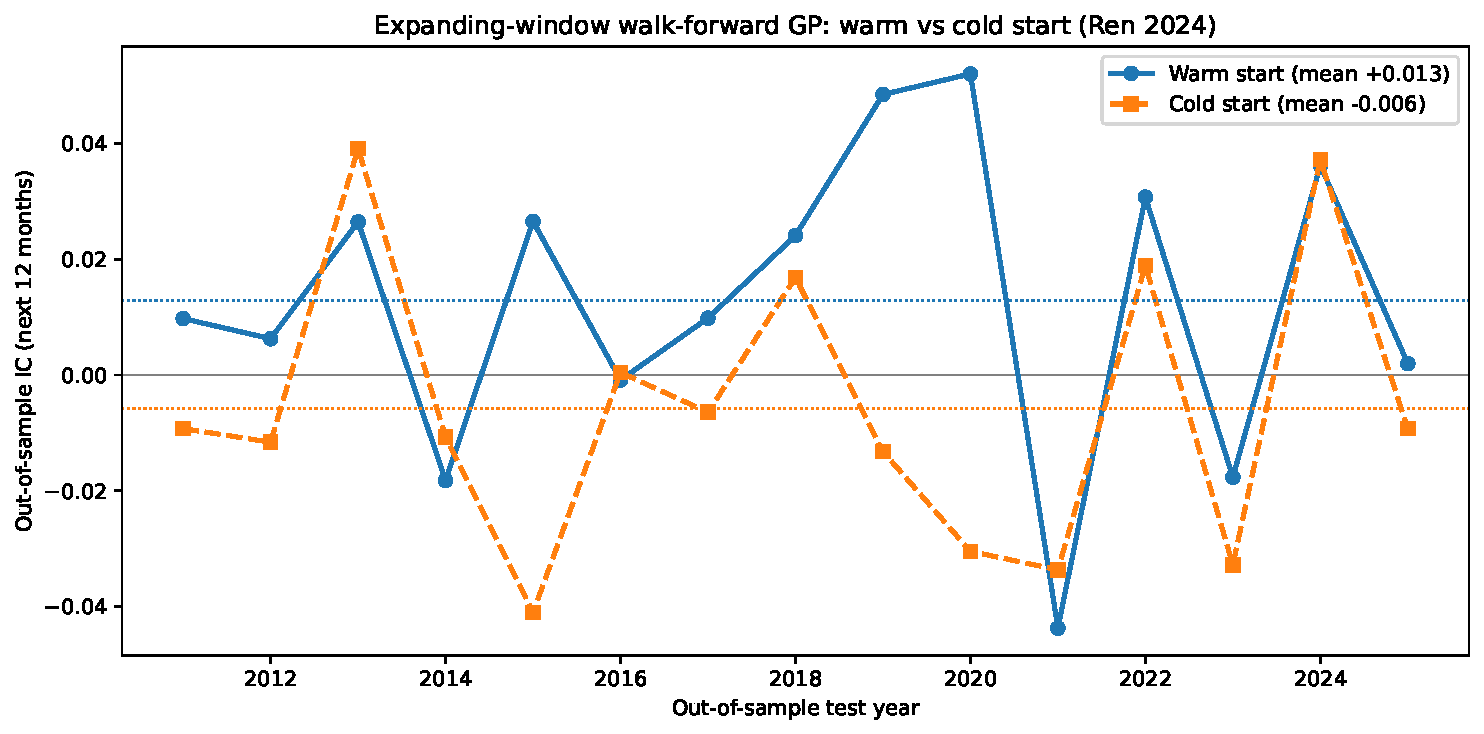
\includegraphics[width=0.7\linewidth]{files/f8620046f620cb3c975abe6358081c56.pdf}

FIGURE 11.13: Out-of-sample IC in each of fifteen yearly test periods (2011 to 2025) for warm-start (solid) versus cold-start (dashed) GP alpha mining, under an expanding training window. Dotted lines mark the means. The warm-started GP is positive in roughly three years out of four; the randomly initialised GP oscillates around zero.

FIGURE 11.13 makes an important methodological point. A single train-test split (for example, training on 2015 to 2019 and testing on 2020 to 2022) would have shown \textit{both} variants failing out of sample, because that particular window straddles the COVID dislocation and the 2021 momentum crash, the worst period for both curves. Averaged over fifteen periods a different picture emerges: warm-starting produces alphas that carry a small but genuine out-of-sample edge (mean IC 0.013, of the same order as the 0.047 Ren et al. report on Chinese A-shares once the difference in universe and horizon is taken into account), whereas random initialisation overfits and delivers no reliable skill. This reinforces the central warning of §11.7.1: out-of-sample validation must span many periods, not one.

\textbf{Optimising the traded objective \citep{Kottas2026}.} \cite{Kottas2026} argues that a GA should optimise the quantity the investor actually trades, not a statistical proxy. We compare three feature subsets: one selected by a GA whose fitness is the top-minus-bottom decile long-short spread, one selected for cross-sectional IC, and the curated short list.

\begin{verbatim}
def decile_spread(mask):
    """Mean monthly top-minus-bottom decile return of the selected composite."""
    comp = signed_z[:, mask].mean(axis=1)
    df = pd.DataFrame({'c': comp, 'r': y, 'dt': dates})
    df['dec'] = df.groupby('dt')['c'].transform(
        lambda s: pd.qcut(s.rank(method='first'), 10, labels=False))
    spread = (df[df.dec == 9].groupby('dt').r.mean()
              - df[df.dec == 0].groupby('dt').r.mean())
    return (spread.mean(),)
\end{verbatim}

\begin{verbatim}
Long-short decile Sharpe (annualised), in-sample / 2020-22 out-of-sample:
Spread-fitness GA:  1.36 / +0.09      IC-fitness GA:  1.48 / -0.17
Curated short list: 0.85 / -0.29
\end{verbatim}

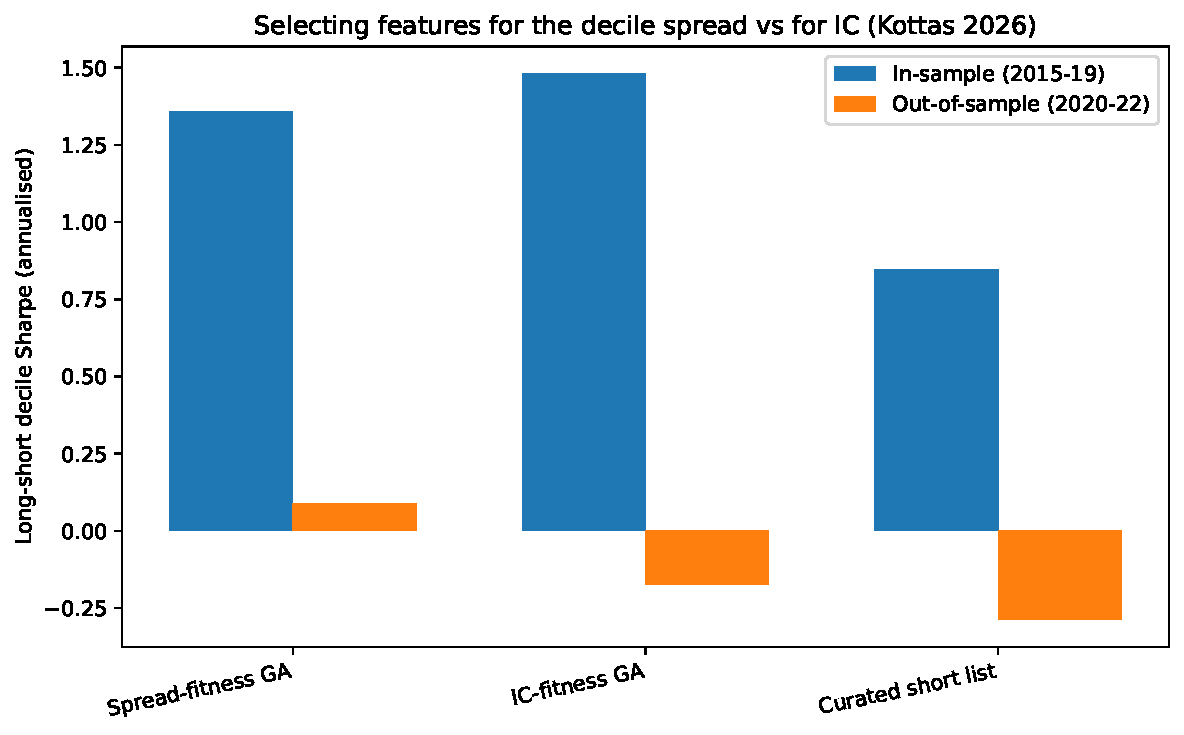
\includegraphics[width=0.7\linewidth]{files/2c4394b91e65d175a4556c6a31d33a27.pdf}

FIGURE 11.14: Annualised long-short decile Sharpe ratio, in-sample (2015 to 2019, blue) and out-of-sample (2020 to 2022, orange), for features chosen to maximise the decile spread, features chosen to maximise IC, and the curated short list. Only the spread-optimised subset stays positive out of sample.

As FIGURE 11.14 shows, the subset selected for the decile spread is the only one of the three with a positive (if modest) out-of-sample Sharpe, even though the IC-optimised subset has the highest \textit{in-sample} Sharpe. Aligning the fitness function with the traded objective, exactly Kottas's argument and an echo of the Sharpe-ratio fitness of Liu et al. (2020, §11.3.2), helps the selection generalise. We stress that this is a single out-of-sample window and therefore only suggestive; the walk-forward protocol behind FIGURE 11.13 would be needed for a firm conclusion.

\textbf{The accuracy-complexity frontier \citep{WangGeng2026}.} Finally, we apply NSGA-II (§11.5.2) to the GP itself, treating alpha discovery as a bi-objective problem: maximise in-sample IC and minimise formula complexity (tree size). This recovers a Pareto front of interpretable alphas of increasing size.

\begin{verbatim}
creator.create("FitMO", base.Fitness, weights=(1.0, -1.0))   # max IC, min tree size
toolbox.register("evaluate", lambda ind: (ic(ind), len(ind)))
toolbox.register("select", tools.selNSGA2)                    # remaining setup as in §11.5.4
\end{verbatim}

\begin{verbatim}
Pareto front (best IC at each complexity):
size 1:  IC 0.025  ->  PB
size 3:  IC 0.033  ->  subtract(PB, mom_22)
size 5:  IC 0.038  ->  subtract(subtract(rel_str_252d, mom_22), Div_yld)
\end{verbatim}

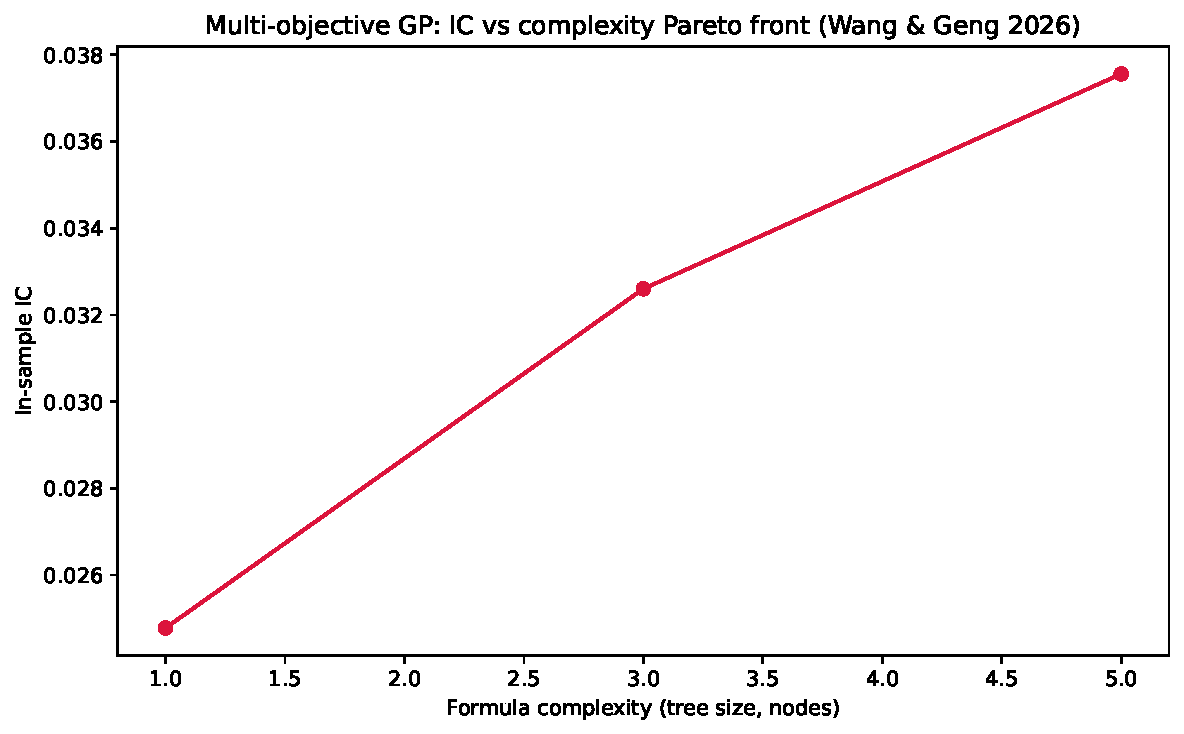
\includegraphics[width=0.7\linewidth]{files/2e3fc035656781263d295a3a0cbda41c.pdf}

FIGURE 11.15: In-sample IC versus formula complexity (tree size in nodes) along the NSGA-II Pareto front. A single value factor (\texttt{PB}) achieves IC 0.025; combining it with momentum lifts this to 0.033, and a three-term expression reaches 0.038, after which added complexity buys no further predictive power.

FIGURE 11.15 traces the interpretability-accuracy trade-off that \cite{WangGeng2026} exploit. The front is short and saturates quickly: beyond about five nodes, larger formulas do not improve IC, so the multi-objective search has no incentive to grow them. For a practitioner this is a useful diagnostic, it identifies the simplest formula that captures most of the available signal, and it guards against the bloat (§11.3.2) that plagues single-objective GP.

\subsubsection{Critical discussion}

\paragraph{The overfitting problem}

Backtest overfitting is the central methodological challenge in GA-based factor research, and it deserves the same careful treatment given to it in Chapter 14 (§14.4.2). The problem is amplified with GAs because they evaluate \textbf{thousands to millions of candidate solutions} over the course of a run, each evaluation is an implicit hypothesis test, and the probability of finding a spuriously good solution increases with the number of evaluations. \cite{harvey2016and} documented that over 300 factors have been proposed in the cross-section literature, many likely spurious; a GA that mines freely over feature combinations exacerbates this multiplicity problem substantially.

Bailey and López de Prado (2014, 2017) developed foundational frameworks for quantifying this risk:

\begin{itemize}
\item \textbf{Probability of Backtest Overfitting (PBO):} measures the probability that the in-sample optimal strategy underperforms the median out-of-sample. A PBO above 50\% is a red flag.
\item \textbf{Deflated Sharpe Ratio (DSR):} adjusts the observed Sharpe ratio for the number of trials, non-normality (skewness and kurtosis), and sample length. The DSR answers: ``given that we tested $N$ strategies, what is the probability that the best Sharpe ratio would arise by chance?''
\item \textbf{Combinatorial Purged Cross-Validation (CPCV):} creates multiple train/test splits that respect temporal ordering and avoid data leakage from autocorrelation. \cite{Arian2024} conducted a comprehensive comparison of out-of-sample testing methods (K-Fold, Purged K-Fold, Walk-Forward, CPCV) in a synthetic controlled environment. Their results demonstrate a \textbf{marked superiority of CPCV} in mitigating overfitting risks, as measured by lower PBO and superior DSR. They additionally propose two extensions (\textit{Bagged CPCV} and \textit{Adaptive CPCV}) that further improve robustness.
\end{itemize}

The overfitting problem is particularly acute for LLM-GA hybrids (§11.4.5), where the LLM's vast parameter space enables the generation of highly complex, seemingly plausible but potentially spurious alpha expressions. \cite{tang2025alphaagent} address this directly with AST-based complexity control and originality enforcement in AlphaAgent. More broadly, the number of implicit hypotheses tested during an evolutionary run grows as $O(N_{\text{pop}} \times N_{\text{gen}})$, which for typical settings (population 100, generations 50) means 5,000+ strategies are implicitly evaluated, a scale that demands the DSR adjustment.

\paragraph{Computational cost}

GAs are inherently more expensive than gradient-based methods because they require evaluating an entire population at each generation. The total number of fitness evaluations is:

\begin{equation}
C = N_{\text{pop}} \times N_{\text{gen}} \times c_{\text{eval}}, \tag{11.7}
\end{equation}

where $c_{\text{eval}}$ is the cost of a single fitness evaluation. For feature selection with cross-validated XGBoost, each evaluation involves training 5 models (5-fold CV), which can take seconds to minutes depending on dataset size. With $N_{\text{pop}} = 50$ and $N_{\text{gen}} = 30$, this amounts to 1,500 model trainings. This is manageable for moderate datasets but potentially prohibitive for large-scale applications.

\textbf{Strategies to reduce computational cost:}

\begin{itemize}
\item \textbf{Surrogate fitness functions:} approximate the true fitness with a cheaper model (connecting to the Bayesian optimisation ideas of §12.3.3).
\item \textbf{Parallel evaluation:} fitness evaluations within a generation are independent and can be distributed across CPU cores or machines.
\item \textbf{Early stopping:} halt evolution when fitness has not improved for a specified number of generations.
\item \textbf{Hierarchical evaluation:} use a cheap fitness (e.g., in-sample IC) for initial screening and an expensive one (e.g., walk-forward Sharpe) only for promising candidates.
\end{itemize}

\cite{Huber2019} demonstrate that GAs can optimise portfolios with over 100,000 time series of 5,000 daily returns, achieving convergence in under five minutes. This suggests that with careful implementation, computational cost is not a fundamental barrier.

\textbf{Use a GA when:}

\begin{itemize}
\item The search space is discrete, combinatorial, or mixed (integer + continuous).
\item The objective function is non-differentiable, noisy, or has many local optima.
\item You need the Pareto front of multiple conflicting objectives.
\item Constraints are complex and heterogeneous (cardinality + turnover + sector limits).
\item You want interpretable solutions (formulaic alphas via GP).
\end{itemize}

\textbf{Prefer other methods when:}

\begin{itemize}
\item The problem is convex (use quadratic programming or gradient descent).
\item The search space is continuous and low-dimensional (use Bayesian optimisation).
\item You need guaranteed optimality (use exact solvers for small problems).
\item Computational budget is extremely tight (use random search as a baseline).
\end{itemize}

\paragraph{Research gaps and future directions}

Despite three decades of research, significant gaps remain. We group the most salient into four themes: the scientific validity of what GAs discover, the breadth of problems to which they are applied, the challenge of scaling the search, and the design of adaptive and hybrid systems.

\textbf{Scientific validity and trustworthiness.} A first cluster of gaps concerns whether evolved solutions can be trusted.

\begin{enumerate}
\item \textbf{Causal versus correlational discovery.} Most GA research identifies statistical associations; few methods distinguish genuine causal factors from spurious correlations. Combining GAs with causal inference methods (Chapter 18) is a promising direction. The \textit{invariance} principle (see §18.1) could be incorporated as a fitness criterion: prefer factors whose predictive power is stable across different market regimes.
\item \textbf{Robustness and reproducibility.} GA results are inherently stochastic: different random seeds produce different solutions. Few papers report confidence intervals across multiple runs, and fewer still share code. The community would benefit from standardised benchmarks and reproducibility protocols, as has been done for neural network research.
\end{enumerate}

\textbf{Broadening the application domain.} A second cluster concerns extending GAs beyond the settings where they are already established.

\begin{enumerate}[resume]
\item \textbf{Alternative data integration.} GA frameworks for satellite imagery, social media sentiment, and transaction data remain underdeveloped. The strongly-typed GP of \cite{Christodoulaki2025}, which handles heterogeneous data types via separate tree branches, offers one promising architectural template.
\item \textbf{Cross-asset applications.} The literature concentrates overwhelmingly on equities; fixed income, commodities, FX, and derivatives receive comparatively little attention. The constrained optimisation abilities of GAs (§11.4.2) would be valuable for fixed-income portfolios, where constraints on duration, sector allocation, and credit quality are pervasive.
\item \textbf{Factor timing via evolutionary rules.} The factor timing literature \citep{neuhierl2023timing} shows that a timed multifactor portfolio achieves approximately 20\% higher returns than its untimed counterpart, with past factor returns and volatility being the best individual predictors. GAs are natural tools for evolving conditional timing rules: ``overweight momentum when trailing volatility is below threshold $\theta_1$ and momentum IC over the past 6 months exceeds $\theta_2$.'' This is a mixed-integer optimisation (continuous thresholds, discrete factor activation) that connects directly to the trading rule evolution of §11.4.5 and the walk-forward framework of §11.6. \cite{Bauer1992} demonstrated the earliest version of this idea, evolving switching strategies between the S\&P 500 and small-firm portfolios.
\end{enumerate}

\textbf{Scaling the search to large problems.} A third cluster concerns the computational barriers that arise as universes and search spaces grow.

\begin{enumerate}[resume]
\item \textbf{Scalability to large universes.} \cite{Huber2019} demonstrated feasibility for 100,000+ time series, most academic studies work with universes of 30 to 500 assets. Scaling multi-objective GAs (§11.5) to global equity universes of 5,000+ stocks, with realistic constraints, remains an open engineering challenge.
\item \textbf{Multi-objective feature selection at scale.} We demonstrated in §11.6.4 that NSGA-II can recover the full IC-vs-parsimony Pareto front for a single training period. Extending this to the walk-forward setting (running NSGA-II at every rebalancing date and tracking how the Pareto front evolves over time) remains computationally expensive and largely unexplored. \cite{Xue2016} provide a comprehensive survey of evolutionary multi-objective feature selection; scaling these methods to high-frequency rebalancing with hundreds of features is an open challenge.
\item \textbf{Cooperative coevolution for grouped features.} With 122 candidate features in §11.6, the search space is 2\textsuperscript{122}. Cooperative coevolution \citep{PotterDeJong2000}, introduced with De Jong, decomposes the problem into subpopulations, each handling a feature group (e.g., all momentum features, all value features, all quality metrics). This leverages the natural category structure of the factor universe described in Chapter 5 and dramatically reduces the effective search space. \cite{Rashid2020} demonstrate that random feature grouping with cooperative coevolution scales effectively to high-dimensional datasets.
\end{enumerate}

\textbf{Adaptive and hybrid architectures.} A final cluster concerns evolutionary systems that adapt over time or couple GAs with other paradigms.

\begin{enumerate}[resume]
\item \textbf{Real-time adaptation.} Limited research addresses online evolutionary systems that adapt to non-stationary markets without full retraining. This connects to the online learning discussion in Chapter 18 (§18.2.2). An evolutionary population that is continuously updated as new data arrives (rather than re-initialised from scratch at each rebalancing date) could reduce computational cost and better track regime changes.
\item \textbf{LLM-evolutionary co-design.} The current LLM-GA hybrids (§11.4.5) treat the LLM and the evolutionary engine as separate modules. A deeper co-design (where the LLM's internal representations are shaped by evolutionary feedback and the evolutionary operators are guided by semantic understanding) is a natural next step. The survey by \cite{ZhangJ2025} identifies this as a key open challenge.
\item \textbf{Quantum-evolutionary computing.} Quantum annealing for combinatorial portfolio problems (cardinality constraints, §11.4.2) is an emerging research frontier that could fundamentally change the computational landscape for GA-hard problems.
\end{enumerate}

\subsubsection{Coding exercises}

\begin{enumerate}
\item \textbf{Multi-objective with turnover.} Extend the NSGA-II application of §11.5.3 to a tri-objective problem: maximise return, minimise volatility, and minimise turnover (measured as the L1 distance from the previous portfolio). Plot the 3D Pareto front and discuss the trade-offs.
\item \textbf{Sensitivity analysis.} Systematically vary the GA parameters (population size $\in \{20, 50, 100, 200\}$, mutation rate $\in \{0.01, 0.02, 0.05, 0.10\}$, number of generations $\in \{20, 50, 100\}$) for the GA feature selection task of §11.4.1. Create a heatmap of out-of-sample IC as a function of these parameters and identify the optimal configuration.
\item \textbf{Weighted factor composites.} Extend the GA feature selection of §11.4.1 by replacing the binary chromosome with a hybrid encoding: a binary gene for inclusion and a real-valued gene for weight for each of the 122 features. Use arithmetic crossover (Equation 11.4) for the weight portion and bit-flip mutation for the binary portion. Compare the out-of-sample IC of the weighted composite against the equal-weighted composite and the short list.
\end{enumerate}

\subsubsection{References}

\section{From predictions to portfolios}

\subsection{Validating and tuning}

% # (PART) From predictions to portfolios {-}

As is shown in Chapters \href{/chap-06-lasso}{Penalized regressions and sparse hedging for minimum variance portfolios} to \href{/chap-14-ensemble}{Ensemble models}, ML models require user-specified choices before they can be trained. These choices encompass parameter values (learning rate, penalization intensity, etc.) or architectural choices (e.g., the structure of a network). Alternative designs in ML engines can lead to different predictions, hence selecting a good one can be critical. We refer to the work of \cite{probst2018tunability} for a study on the impact of hyperparameter tuning on model performance. For some models (neural networks and boosted trees), the number of degrees of freedom is so large that finding the right parameters can become complicated and challenging. This chapter addresses these issues but the reader must be aware that there is no shortcut to building good models. Crafting an effective model is time-consuming and often the result of many iterations.

\subsubsection{Learning metrics}

The parameter values that are set before training are called \textbf{hyperparameters}. In order to be able to choose good hyperparameters, it is imperative to define metrics that evaluate the performance of ML models. As is often the case in ML, there is a dichotomy between models that seek to predict numbers (regressions) and those that try to forecast categories (classifications). Before we outline common evaluation benchmarks, we mention the econometric approach of \cite{li2020conditional}. The authors propose to assess the performance of a forecasting method compared to a given benchmark, \textbf{conditional} on some external variable. This helps monitor under which (economic) conditions the model beats the benchmark. The full implementation of the test is intricate, and we recommend the interested reader have a look at the derivations in the paper.

\paragraph{Regression analysis}

Errors in regression analyses are usually evaluated in a straightforward way. The $L^1$ and $L^2$ norms are mainstream; they are both easy to interpret and to compute. The second one, the root \textbf{mean squared error} (RMSE) is differentiable everywhere but harder to grasp and gives more weight to outliers. The first one, the mean absolute error gives the average distance to the realized value but is not differentiable at zero. Formally, we define them as

\begin{equation}
\label{eq-MAE}
\text{MAE}(\textbf{y},\tilde{\textbf{y}})=\frac{1}{I}\sum_{i=1}^I|y_i-\tilde{y}_i|,
\end{equation}

\begin{equation}
\label{eq-MSE}
\text{MSE}(\textbf{y},\tilde{\textbf{y}})=\frac{1}{I}\sum_{i=1}^I(y_i-\tilde{y}_i)^2,
\end{equation}

and the RMSE is simply the square root of the MSE. It is always possible to generalize these formulae by adding weights $w_i$ to produce heterogeneity in the importance of instances. Let us briefly comment on the MSE. It is by far the most common loss function in machine learning, but it is not necessarily the exact best choice for return prediction in a portfolio allocation task. If we decompose the loss into its 3 terms, we get the sum of squared realized returns, the sum of squared predicted returns and the product between the two (roughly speaking, a covariance term if we assume zero means). The first term does not matter. The second controls the dispersion around zero of the predictions. The third term is the most interesting from the allocator's standpoint. The negativity of the cross-product $-2y_i\tilde{y}_i$ is always to the investor's benefit: either both terms are positive and the model has recognized a profitable asset, or they are negative and it has identified a bad opportunity. It is when $y_i$ and $\tilde{y}_i$ don't have the same sign that problems arise. Thus, compared to the $\tilde{y}_i^2$, the cross-term is more important. Nonetheless, algorithms do not optimize with respect to this indicator.\footnote{There are some exceptions, like attempts to optimize more exotic criteria, such as the Spearman rho, which is based on rankings and is close in spirit to maximizing the correlation between the output and the prediction. Because this rho cannot be differentiated, this causes numerical issues. These problems can be partially alleviated when resorting to complex architectures, as in \cite{engilberge2019sodeep}.}

These metrics (MSE and RMSE) are widely used outside ML to assess forecasting errors. Below, we present other indicators that are also sometimes used to quantify the quality of a model. In line with the linear regressions, the $R^2$ can be computed in any predictive exercise.

\begin{equation}
\label{eq-R2}
R^2(\textbf{y},\tilde{\textbf{y}})=1- \frac{\sum_{i=1}^I(y_i-\tilde{y}_i)^2}{\sum_{i=1}^I(y_i-\bar{y})^2},
\end{equation}

where $\bar{y}$ is the sample average of the label. One important difference with the classical $R^2$ is that the above quantity can be computed on the \textbf{testing sample} and not on the \textbf{training sample}. In this case, the $R^2$ can be negative when the mean squared error in the numerator is larger than the (biased) variance of the testing sample. Sometimes, the average value $\bar{y}$ is omitted in the denominator (as in \cite{gu2018empirical} for instance). The benefit of removing the average value is that it compares the predictions of the model to a zero prediction. This is particularly relevant with returns because the simplest prediction of all is the constant zero value and the $R^2$ can then measure if the model beats this naive benchmark. A zero prediction is always preferable to a sample average because the latter can be very much period dependent. Also, removing $\bar{y}$ in the denominator makes the metric more conservative as it mechanically reduces the $R^2$.

Beyond the simple indicators detailed above, several exotic extensions exist and they all consist in altering the error before taking the averages. Two notable examples are the Mean Absolute Percentage Error (MAPE) and the Mean Square Percentage Error (MSPE). Instead of looking at the raw error, they compute the error relative to the original value (to be predicted). Hence, the error is expressed in a percentage score and the averages are simply equal to:

\begin{equation}
\label{eq-MAPE}
\text{MAPE}(\textbf{y},\tilde{\textbf{y}})=\frac{1}{I}\sum_{i=1}^I\left|\frac{y_i-\tilde{y}_i}{y_i}\right|,
\end{equation}

\begin{equation}
\label{eq-MSPE}
\text{MSPE}(\textbf{y},\tilde{\textbf{y}})=\frac{1}{I}\sum_{i=1}^I\left(\frac{y_i-\tilde{y}_i}{y_i}\right)^2,
\end{equation}

where the latter can be scaled by a square root if need be. When the label is positive with possibly large values, it is possible to scale the magnitude of errors, which can be very large. One way to do this is to resort to the Root Mean Squared Logarithmic Error (RMSLE), defined below:

\begin{equation}
\label{eq-RMSLE}
\text{RMSLE}(\textbf{y},\tilde{\textbf{y}})=\sqrt{\frac{1}{I}\sum_{i=1}^I\log\left(\frac{1+y_i}{1+\tilde{y}_i}\right)},
\end{equation}

where it is obvious that when $y_i=\tilde{y}_i$, the error metric is equal to zero.

Before we move on to categorical losses, we briefly comment on one shortcoming of the MSE, which is by far the most widespread metric and objective in regression tasks. A simple decomposition yields:

\begin{equation}
\text{MSE}(\textbf{y},\tilde{\textbf{y}})=\frac{1}{I}\sum_{i=1}^I(y_i^2+\tilde{y}_i^2-2y_i\tilde{y}_i).
\end{equation}

In the sum, the first term is given, there is nothing to be done about it, hence models focus on the minimization of the other two. The second term is the dispersion of model values. The third term is a cross-product. While variations in $\tilde{y}_i$ do matter, the third term is by far the most important, especially in the cross-section. It is more valuable to reduce the MSE by increasing $y_i\tilde{y}_i$. This product is indeed positive when the two terms have the same sign, which is exactly what an investor is looking for: \textbf{correct directions} for the bets. For some algorithms (like neural networks), it is possible to manually specify custom losses. Maximizing the sum of $y_i\tilde{y}_i$ may be a good alternative to vanilla quadratic optimization (see Section~\ref{custloss} for an example of implementation).

\paragraph{Classification analysis}

The performance metrics for categorical outcomes are substantially different compared to those of numerical outputs. A large proportion of these metrics are dedicated to binary classes, though some of them can easily be generalized to multiclass models.

We present the concepts pertaining to these metrics in an increasing order of complexity and start with the two dichotomies true versus false and positive versus negative. In binary classification, it is convenient to think in terms of true versus false. In an investment setting, true can be related to a positive return, or a return being above that of a benchmark - false being the opposite.

There are then 4 types of possible results for a prediction. Two when the prediction is right (predict true with true realization or predict false with false outcome) and two when the prediction is wrong (predict true with false realization and the opposite). We define the corresponding aggregate metrics below:

\begin{itemize}
\item frequency of true positive: $TP=I^{ -1}\sum_{i=1}^I1_{\{y_i=\tilde{y}_i=1 \}},$
\item frequency of true negative: $TN=I^{ -1}\sum_{i=1}^I1_{\{y_i=\tilde{y}_i=0 \}},$
\item frequency of false positive: $FP=I^{ -1}\sum_{i=1}^I1_{\{\tilde{y}_i=1,y_i=0 \}},$
\item frequency of false negative: $FN=I^{ -1}\sum_{i=1}^I1_{\{\tilde{y}_i=0,y_i=1 \}},$
\end{itemize}

where true is conventionally encoded into 1 and false into 0. The sum of the four figures is equal to one. These four numbers have very different impacts on out-of-sample results, as is shown in Figure~\ref{fig-valconfusion}. In this table (also called a \textbf{confusion matrix}), it is assumed that some proxy for future profitability is forecast by the model. Each row stands for the model's prediction and each column for the realization of the profitability. The most important cases are those in the top row, when the model predicts a positive result because it is likely that assets with positive predicted profitability (possibly relative to some benchmark) will end up in the portfolio. Of course, this is not a problem if the asset does well (left cell), but it becomes penalizing if the model is wrong because the portfolio will suffer.

\begin{figure}[!htbp]
\centering
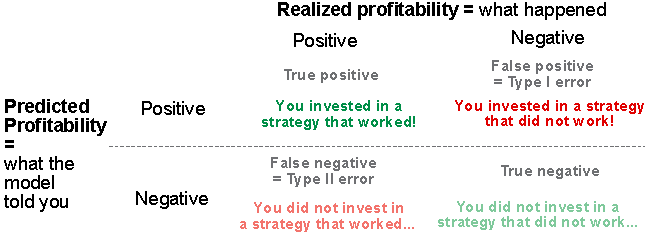
\includegraphics[width=0.7\linewidth]{files/confusion-2f45b9249d2c033e4756e0e164d778fb.pdf}
\caption[]{Confusion matrix: summary of binary outcomes.}
\label{fig-valconfusion}
\end{figure}

Among the two types of errors, \textbf{type I} is the most daunting for investors because it has a direct effect on the portfolio. The \textbf{type II} error is simply a missed opportunity and is somewhat less impactful. Finally, true negatives are those assets which are correctly excluded from the portfolio.

From the four baseline rates, it is possible to derive other interesting metrics:

\begin{itemize}
\item \textbf{Accuracy} = $TP+TN$ is the percentage of correct forecasts;
\item \textbf{Recall} = $\frac{TP}{TP+FN}$ measures the ability to detect a winning strategy/asset (left column analysis). Also known as sensitivity or true positive rate (TPR);
\item \textbf{Precision} = $\frac{TP}{TP+FP}$ computes the probability of good investments (top row analysis);
\item \textbf{Specificity} = $\frac{TN}{FP+TN}$ measures the proportion of actual negatives that are correctly identified as such (right column analysis);
\item \textbf{Fallout} = $\frac{FP}{FP+TN}=1 -$Specificity is the probability of false alarm (or false positive rate), i.e., the frequence at which the algorithm detects falsely performing assets (right column analysis);
\item \textbf{F-score}, $\mathbf{F}_1=2\frac{\text{recall}\times \text{precision}}{\text{recall}+ \text{precision}}$ is the harmonic average of recall and precision.
\end{itemize}

All of these items lie in the unit interval and a model is deemed to perform better when they increase (except for fallout for which it is the opposite). Many other indicators also exist, like the false discovery rate or false omission rate, but they are not as mainstream and less cited. Moreover, they are often simple functions of the ones mentioned above.

A metric that is popular but more complex is the Area Under the (ROC) Curve, often referred to as AUC. The complicated part is the ROC curve where ROC stands for Receiver Operating Characteristic; the name comes from signal theory. We explain how it is built below.

As seen in Chapters \href{/chap-07-trees}{Tree-based methods} and \href{/chap-08-neural-networks}{Neural networks}, classifiers generate output that are probabilities that one instance belongs to one class. These probabilities are then translated into a class by choosing the class that has the highest value. In binary classification, the class with a score above 0.5 basically wins.

In practice, this 0.5 threshold may not be optimal and the model could very well correctly predict false instances when the probability is below 0.4 and true ones otherwise. Hence, it is a natural idea to test what happens if the decision threshold changes. The ROC curve does just that and plots the recall as a function of the fallout when the threshold increases from zero to one.

When the threshold is equal to 0, true positives are equal to zero because the model never forecasts positive values. Thus, both recall and fallout are equal to zero. When the threshold is equal to one, false negatives shrink to zero and true negatives too, hence recall and fallout are equal to one. The behavior of their relationship in between these two extremes is called the \textbf{ROC curve}. We provide stylized examples below in Figure~\ref{fig-ROCcurve}. A random classifier would fare equally good for recall and fallout and thus the ROC curve would be a linear line from the point (0,0) to (1,1). To prove this, imagine a sample with a $p\in (0,1)$ proportion of true instances and a classifier that predicts true randomly with a probability $p'\in (0,1)$. Then because the sample and predictions are independent, $TP=p'p$, $FP = p'(1 -p)$, $TN=(1 -p')(1 -p)$ and $FN=(1 -p')p$. Given the above definition, this yields that both recall and fallout are equal to $p'$.

\begin{figure}[!htbp]
\centering
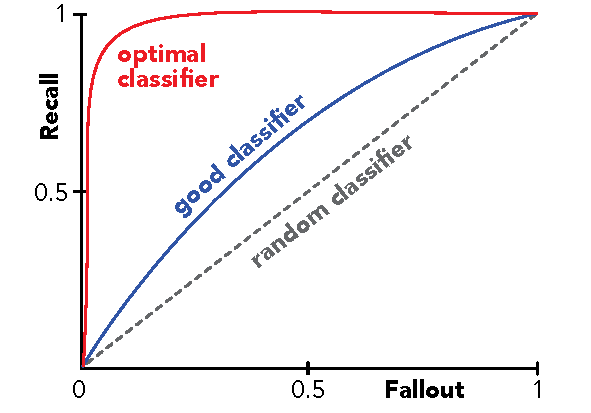
\includegraphics[width=0.7\linewidth]{files/ROCcurve-b0fc90e34ebc722ade14908f8f5f3f45.pdf}
\caption[]{Stylized ROC curves.}
\label{fig-ROCcurve}
\end{figure}

An algorithm with a ROC curve above the 45° angle is performing better than an average classifier. Indeed, the curve can be seen as a tradeoff between benefits (probability of detecting good strategies on the $y$ axis) minus costs (odds of selecting the wrong assets on the $x$ axis). Hence being above the 45° is paramount. The best possible classifier has a ROC curve that goes from point (0,0) to point (0,1) to point (1,1). At point (0,1), fallout is null, hence there are no false positives, and recall is equal to one so that there are also no false negatives: the model is always right. The opposite is true: at point (1,0), the model is always wrong.

Below, we use sklearn to compute and display a ROC curve for a given set of predictions on the testing sample.

\begin{verbatim}
from sklearn.tree import DecisionTreeRegressor, plot_tree
from sklearn.ensemble import RandomForestClassifier
from sklearn.metrics import roc_curve, auc, RocCurveDisplay
from sklearn.linear_model import Ridge
import xgboost as xgb
import numpy as np
import pandas as pd
import matplotlib.pyplot as plt
import seaborn as sns
from itertools import product
import warnings
warnings.filterwarnings('ignore')
plt.style.use('seaborn-v0_8-whitegrid')
sns.set_palette("husl")

# Building the data & import functions
from data_build import generate_data
data_ml, features, features_short, returns, stock_ids, stock_ids_short = generate_data()
features_short = ["Div_yld", "EPS", "size_avg_252d", "mom_252", "OCF_Growth_1Y", "PB", "vol_252"]
separation_date = "2017-01-15"

data_ml_clean = data_ml.dropna(subset=(features_short + ['R1M']))
training_sample = data_ml_clean[data_ml_clean['date'] <= separation_date]
testing_sample = data_ml_clean[data_ml_clean['date'] > separation_date]
\end{verbatim}

\begin{figure}[!htbp]
\centering
\begin{verbatim}
# Prepare data for classification
X_train = training_sample[features_short]
y_train_C = training_sample['R1M_C']
X_test = testing_sample[features_short]
y_test_C = testing_sample['R1M_C']

# Train Random Forest Classifier (similar to fit_RF_C from chapter 6)
fit_RF_C = RandomForestClassifier(
    n_estimators=40,
    max_samples=20000,
    bootstrap=True,
    min_samples_leaf=250,
    max_features=5,
    random_state=42
)
fit_RF_C.fit(X_train, y_train_C)

# Get predicted probabilities for the positive class
y_proba = fit_RF_C.predict_proba(X_test)[:, 1]

# Calculate ROC curve
fpr, tpr, thresholds = roc_curve(y_test_C, y_proba)
roc_auc = auc(fpr, tpr)

# Plot ROC curve
plt.figure(figsize=(6, 5))
plt.plot(fpr, tpr, color='blue', lw=2, label=f'ROC curve (AUC = {roc_auc:.3f})')
plt.plot([0, 1], [0, 1], color='gray', lw=1, linestyle='--', label='Random classifier')
plt.xlim([0.0, 1.0])
plt.ylim([0.0, 1.05])
plt.xlabel('False Positive Rate (Fallout)')
plt.ylabel('True Positive Rate (Recall)')
plt.title('ROC Curve')
plt.legend(loc='lower right')
plt.tight_layout()
plt.show()
\end{verbatim}
\caption[]{Example of ROC curve.

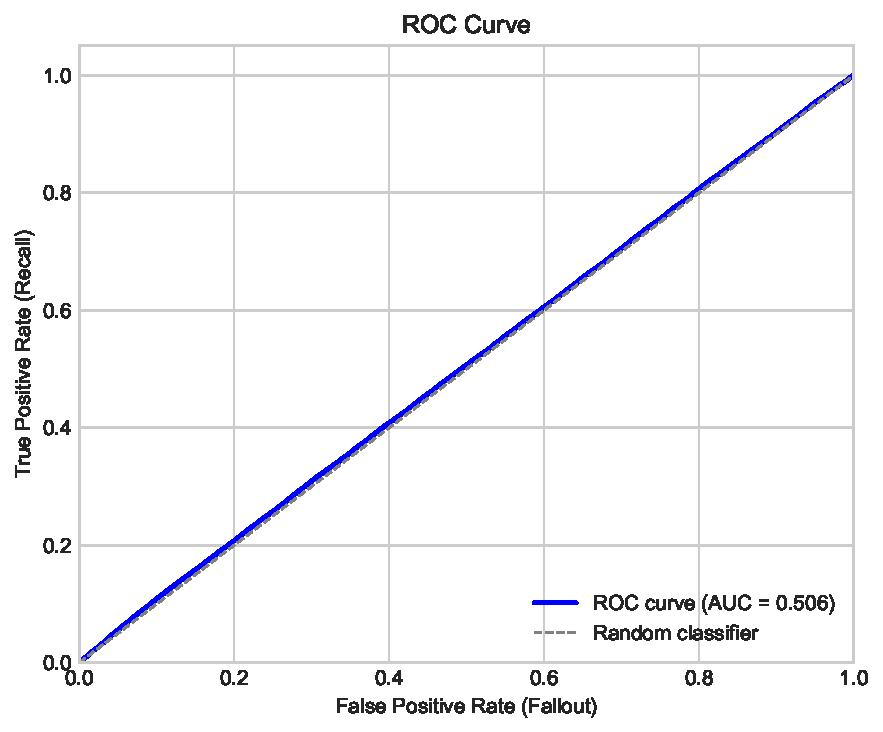
\includegraphics[width=0.7\linewidth]{files/150b2c9337c353f5fc5aefb3bf467be3.pdf}}
\label{fig-roc}
\end{figure}

\begin{verbatim}
print(f"AUC: {roc_auc:.4f}")
\end{verbatim}

\begin{verbatim}
AUC: 0.5063
\end{verbatim}

In Figure~\ref{fig-roc}, the curve is very close to the 45° angle and the model seems as good (or, rather, as bad) as a random classifier.

Finally, having one entire curve is not practical for comparison purposes, hence the information of the whole curve is synthesized into the area below the curve, i.e., the integral of the corresponding function. The 45° angle (quadrant bisector) has an area of 0.5 (it is half the unit square which has a unit area). Thus, any good model is expected to have an area under the curve (AUC) above 0.5. A perfect model has an AUC of one.

We end this subsection with a word on multiclass data. When the output (i.e., the label) has more than two categories, things become more complex. It is still possible to compute a confusion matrix, but the dimension is larger and harder to interpret. The simple indicators like $TP$, $TN$, etc., must be generalized in a non-standard way. The simplest metric in this case is the cross-entropy defined in Equation \ref{eq-crossentropy}. We refer to Section~\ref{sec_treeclass} for more details on losses related to categorical labels.

\subsubsection{Validation}

Validation is the stage at which a model is tested and tuned before it starts to be deployed on real or live data (e.g., for trading purposes). Needless to say, it is critical.

\paragraph{The variance-bias tradeoff: theory}

The \textbf{variance-bias tradeoff} is one of the core concepts in supervised learning. To explain it, let us assume that the data is generated by the simple model

\begin{equation}
y_i=f(\textbf{x}_i)+\epsilon_i, \quad   \mathbb{E}[\boldsymbol{\epsilon}]=0, \quad \mathbb{V}[\boldsymbol{\epsilon}]=\sigma^2,
\end{equation}

but the model that is estimated yields

\begin{equation}
y_i=\hat{f}(\textbf{x}_i)+\hat{\epsilon}_i.
\end{equation}

Given an unknown sample $\textbf{x}$, the decomposition of the average squared error is

\begin{equation}
\label{eq-biasvariance}
\begin{aligned}
\mathbb{E}[\hat{\epsilon}^2]&=\mathbb{E}[(y-\hat{f}(\textbf{x}))^2]=\mathbb{E}[(f(\textbf{x})+\epsilon-\hat{f}(\textbf{x}))^2]   \\
&= \underbrace{\mathbb{E}[(f(\textbf{x})-\hat{f}(\textbf{x}))^2]}_{\text{total quadratic error}}+\underbrace{\mathbb{E}[\epsilon^2]}_{\text{irreducible error}} \\
&= \mathbb{E}[\hat{f}(\textbf{x})^2]+\mathbb{E}[f(\textbf{x})^2]-2\mathbb{E}[f(\textbf{x})\hat{f}(\textbf{x})]+\sigma^2\\
&=\mathbb{E}[\hat{f}(\textbf{x})^2]+f(\textbf{x})^2-2f(\textbf{x})\mathbb{E}[\hat{f}(\textbf{x})]+\sigma^2\\
&=\left[ \mathbb{E}[\hat{f}(\textbf{x})^2]-\mathbb{E}[\hat{f}(\textbf{x})]^2\right]+\left[\mathbb{E}[\hat{f}(\textbf{x})]^2+f(\textbf{x})^2-2f(\textbf{x})\mathbb{E}[\hat{f}(\textbf{x})]\right]+\sigma^2\\
&=\underbrace{\mathbb{V}[\hat{f}(\textbf{x})]}_{\text{variance of model}}+ \quad \underbrace{\mathbb{E}[(f(\textbf{x})-\hat{f}(\textbf{x}))]^2}_{\text{squared bias}}\quad +\quad\sigma^2
\end{aligned}
\end{equation}

In the above derivation, $f(x)$ is not random, but $\hat{f}(x)$ is. Also, in the second line, we assumed $\mathbb{E}[\epsilon(f(x) -\hat{f}(x))]=0$, which may not always hold (though it is a very common assumption). The average squared error thus has three components:

\begin{itemize}
\item the variance of the model (over its predictions);
\item the squared bias of the model;
\item and one \textbf{irreducible error} (independent from the choice of a particular model).
\end{itemize}

The last one is immune to changes in models, so the challenge is to minimize the sum of the first two. This is known as the variance-bias tradeoff because reducing one often leads to increasing the other. The goal is thus to assess when a small increase in either one can lead to a larger decrease in the other.

There are several ways to represent this tradeoff and we display two of them. The first one relates to archery (see Figure~\ref{fig-archery}) below. The best case (top left) is when all shots are concentrated in the middle: on average, the archer aims correctly and all the arrows are very close to one another. The worst case (bottom right) is the exact opposite: the average arrow is above the center of the target (the bias is nonzero) and the dispersion of arrows is large.

\begin{figure}[!htbp]
\centering
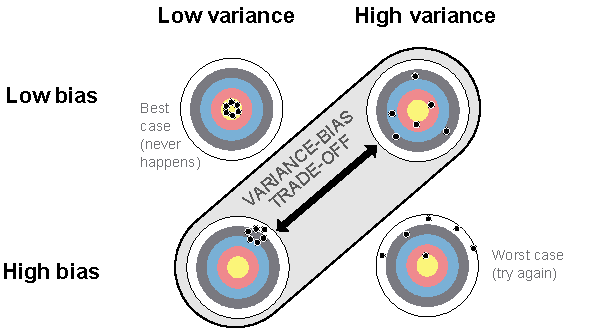
\includegraphics[width=0.7\linewidth]{files/var_bias_trade-396ec89d9182d2200cf2b81c237fe440.pdf}
\caption[]{First representation of the variance-bias tradeoff.}
\label{fig-archery}
\end{figure}

The most often encountered cases in ML are the other two configurations: either the arrows (predictions) are concentrated in a small perimeter, but the perimeter is not the center of the target; or the arrows are on average well distributed around the center, but they are, on average, far from it.

The second way the variance bias tradeoff is often depicted is via the notion of \textbf{model complexity}. The most simple model of all is a constant one: the prediction is always the same, for instance equal to the average value of the label in the training set. Of course, this prediction will often be far from the realized values of the testing set (its bias will be large), but at least its variance is zero. On the other side of the spectrum, a decision tree with as many leaves as there are instances has a very complex structure. It will probably have a smaller bias, but undoubtedly it is not obvious that this will compensate the increase in variance incurred by the intricacy of the model.

This facet of the tradeoff is depicted in Figure~\ref{fig-varbiastrade} below. To the left of the graph, a simple model has a small variance but a large bias, while to the right it is the opposite for a complex model. Good models often lie somewhere in the middle, but the best mix is hard to find.

\begin{figure}[!htbp]
\centering
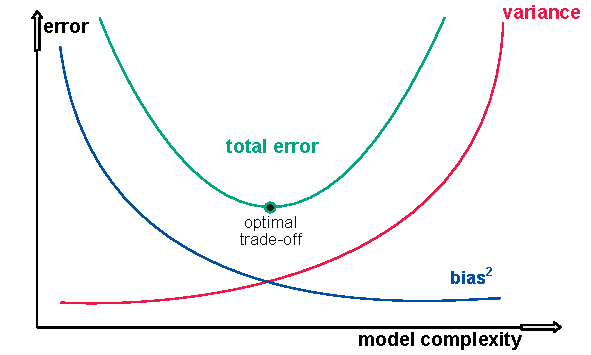
\includegraphics[width=0.7\linewidth]{files/var_bias_trade2-a7da616120ba327b6acf36916bc1f4ee.pdf}
\caption[]{Second representation of the variance-bias tradeoff.}
\label{fig-varbiastrade}
\end{figure}

The most tractable theoretical form of the variance-bias tradeoff is the ridge regression.\footnote{Another angle, critical of neural networks is provided in \cite{geman1992neural}.} The coefficient estimates in this type of regression are given by $\hat{\mathbf{b}}_\lambda=(\mathbf{X}'\mathbf{X}+\lambda \mathbf{I}_N)^{ -1}\mathbf{X}'\mathbf{Y}$ (see Section~\ref{penreg}), where $\lambda$ is the penalization intensity. Assuming a \textit{true} linear form for the data generating process ($\textbf{y}=\textbf{Xb}+\boldsymbol{\epsilon}$ where $\textbf{b}$ is unknown and $\sigma^2$ is the variance of errors - which have identity correlation matrix), this yields

\begin{equation}
\label{eq-vartrade}
\begin{aligned}  
\mathbb{E}[\hat{\textbf{b}}_\lambda]&=\textbf{b}-\lambda(\textbf{X}'\textbf{X}+\lambda \textbf{I}_N)^{-1} \textbf{b}, \\
\mathbb{V}[\hat{\textbf{b}}_\lambda]&=\sigma^2(\textbf{X}'\textbf{X}+\lambda \textbf{I}_N)^{-1}\textbf{X}'\textbf{X}   (\textbf{X}'\textbf{X}+\lambda \textbf{I}_N)^{-1}.
\end{aligned}
\end{equation}

Basically, this means that the bias of the estimator is equal to $-\lambda(\textbf{X}'\textbf{X}+\lambda \textbf{I}_N)^{ -1} \textbf{b}$, which is zero in the absence of penalization (classical regression) and converges to some finite number when $\lambda \rightarrow \infty$, i.e., when the model becomes constant. Note that if the estimator has a zero bias, then predictions will too: $\mathbb{E}[\textbf{X}(\textbf{b} -\hat{\textbf{b}})]=\textbf{0}$.

The variance (of estimates) in the case of an unconstrained regression is equal to $\mathbb{V}[\hat{\textbf{b}}]=\sigma (\textbf{X}'\textbf{X})^{ -1}$. In Equation \ref{eq-vartrade}, the $\lambda$ reduces the magnitude of figures in the inverse matrix. The overall effect is that as $\lambda$ increases, the variance decreases and in the limit $\lambda \rightarrow \infty$, the variance is zero when the model is constant. The variance of predictions is

\begin{equation}
\begin{aligned}
\mathbb{V}[\textbf{X}\hat{\textbf{b}}]&=\mathbb{E}[(\textbf{X}\hat{\textbf{b}}-\mathbb{E}[\textbf{X}\hat{\textbf{b}}])(\textbf{X}\hat{\textbf{b}}-\mathbb{E}[\textbf{X}\hat{\textbf{b}}])'] \\
&= \textbf{X}\mathbb{E}[(\hat{\textbf{b}}-\mathbb{E}[\hat{\textbf{b}}])(\hat{\textbf{b}}-\mathbb{E}[\hat{\textbf{b}}])']\textbf{X}' \\
&= \textbf{X}\mathbb{V}[\hat{\textbf{b}}]\textbf{X}
\end{aligned}
\end{equation}

All in all, ridge regressions are very handy because with a single parameter, they are able to provide a cursor that directly tunes the variance-bias tradeoff.

It's easy to illustrate how simple it is to display the tradeoff with the ridge regression. In the example below, we train ridge models with multiple lambda values.

\begin{figure}[!htbp]
\centering
\begin{verbatim}
# Prepare data for ridge regression
x_penalized_train = training_sample[features_short].values
y_penalized_train = training_sample['R1M'].values
x_penalized_test = testing_sample[features_short].values
y_penalized_test = testing_sample['R1M'].values

# Range of lambda values
lambdas = np.logspace(-4, 4, 100)

# Store predictions for each lambda
predictions_all = np.zeros((len(y_penalized_test), len(lambdas)))

for i, lam in enumerate(lambdas):
    ridge = Ridge(alpha=lam, fit_intercept=True)
    ridge.fit(x_penalized_train, y_penalized_train)
    predictions_all[:, i] = ridge.predict(x_penalized_test)

# Calculate errors, bias, and variance for each lambda
errors = predictions_all - y_penalized_test.reshape(-1, 1)
ridge_bias = errors.mean(axis=0)          # Bias
ridge_var = predictions_all.var(axis=0)   # Variance of predictions

# Plot error decomposition
plt.figure(figsize=(8, 5))
plt.plot(lambdas, ridge_bias**2, label='Squared Bias', linewidth=2)
plt.plot(lambdas, ridge_var, label='Variance', linewidth=2)
plt.plot(lambdas, ridge_bias**2 + ridge_var, label='Total (Bias² + Variance)', linewidth=2, linestyle='--')
plt.xscale('log')
plt.xlabel('Lambda')
plt.ylabel('Value')
plt.legend()
plt.tight_layout()
plt.show()
\end{verbatim}
\caption[]{Error decomposition for a ridge regression.

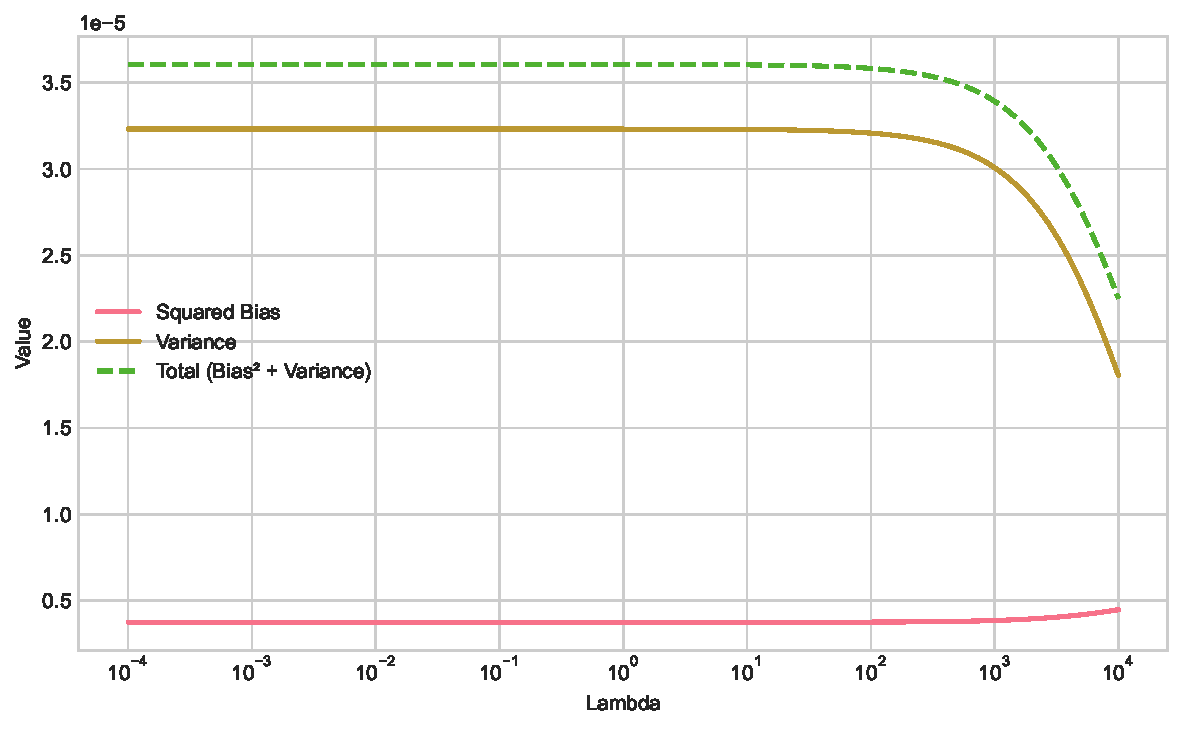
\includegraphics[width=0.7\linewidth]{files/5a6065b3aef0852c0767dce43cc56e6a.pdf}}
\label{fig-ridgetrade}
\end{figure}

In Figure~\ref{fig-ridgetrade}, the pattern is different from the one depicted in Figure~\ref{fig-varbiastrade}. In the graph, when the intensity lambda increases, the magnitude of parameters shrinks and the model becomes simpler. Hence, the most simple model seems like the best choice: adding complexity increases variance but does not improve the bias! One possible reason for that is that features don't actually carry much predictive value and hence a constant model is just as good as more sophisticated ones based on irrelevant variables.

\paragraph{The variance-bias tradeoff: illustration}

The variance-bias tradeoff is often presented in theoretical terms that are easy to grasp. It is nonetheless useful to demonstrate how it operates on true algorithmic choices. Below, we take the example of trees because their complexity is easy to evaluate. Basically, a tree with many terminal nodes is more complex than a tree with a handful of clusters.

We start with the parsimonious model, which we train below.

\begin{figure}[!htbp]
\centering
\begin{verbatim}
# Prepare training data
X_train = training_sample[features_short]
y_train = training_sample['R1M']
X_test = testing_sample[features_short]
y_test = testing_sample['R1M']

# Train a simple tree with max_depth=2
fit_tree_simple = DecisionTreeRegressor(
    ccp_alpha=0.0001,   # Complexity parameter: smaller = more leaves
    max_depth=2         # Maximum depth (i.e. tree levels)
)
fit_tree_simple.fit(X_train, y_train)

# Plot the tree
plt.figure(figsize=(16, 8))
plot_tree(fit_tree_simple, feature_names=features_short, filled=True, rounded=True, fontsize=10)
plt.tight_layout()
plt.show()
\end{verbatim}
\caption[]{Simple tree.

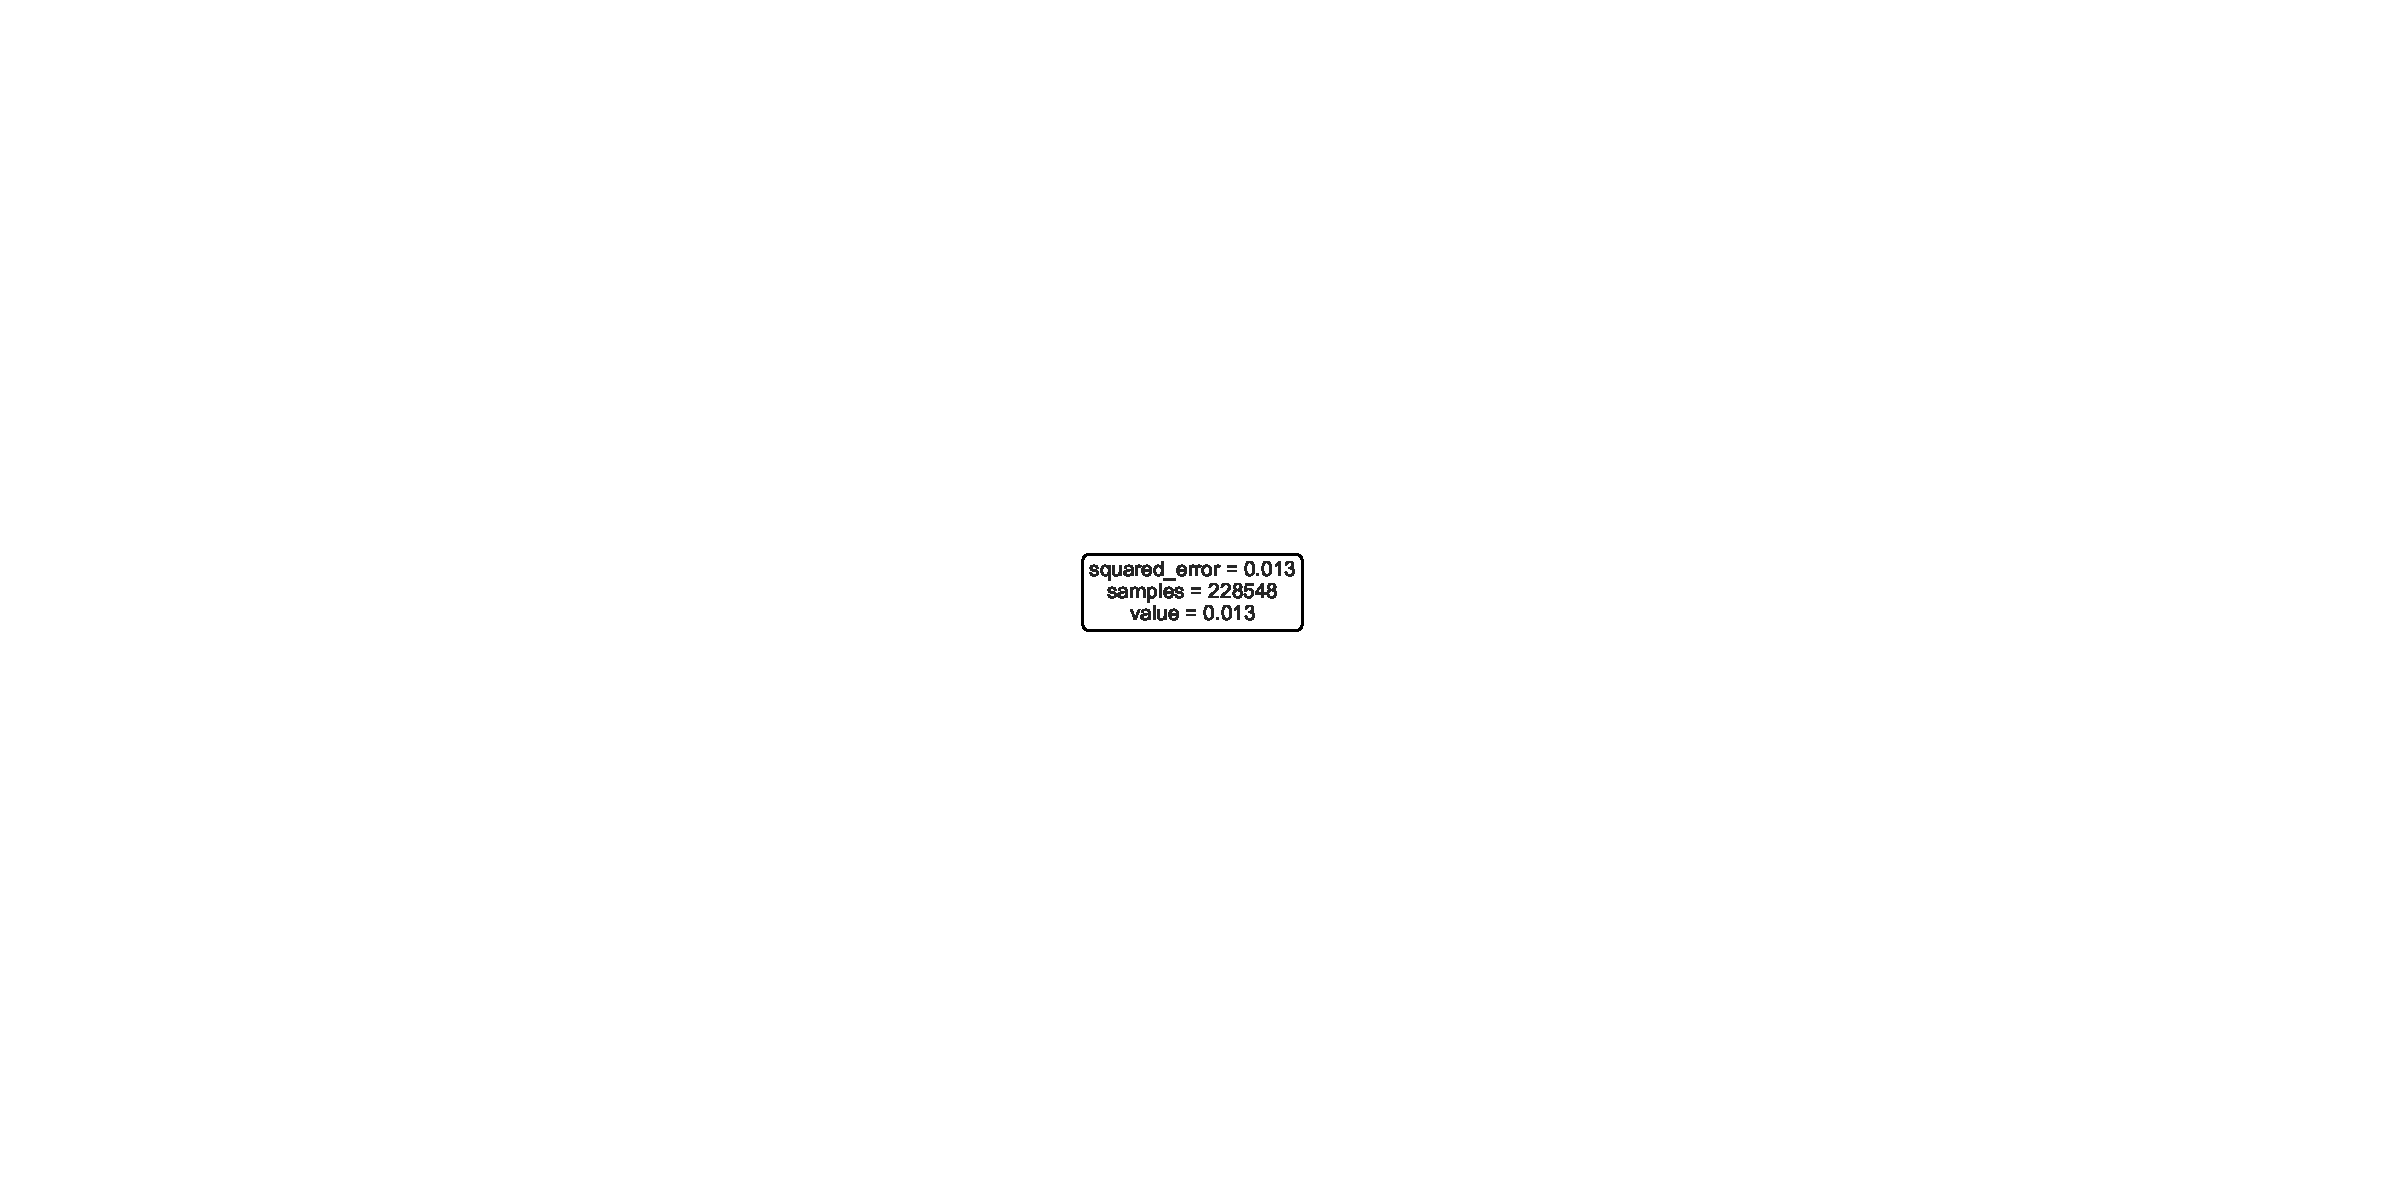
\includegraphics[width=0.7\linewidth]{files/767c4bdb17e8849a3443eca8b134e005.pdf}}
\label{fig-treesimple}
\end{figure}

The model depicted in Figure~\ref{fig-treesimple} only has 4 clusters, which means that the predictions can only take four values. The smallest one encompasses a large portion of the sample and the largest one corresponds to only a small fraction of the training sample.

We are then able to compute the bias and the variance of the predictions on the \textit{testing} set.

\begin{verbatim}
# Bias and variance for simple tree
predictions_simple = fit_tree_simple.predict(X_test)
bias_simple = np.mean(predictions_simple - y_test)
var_simple = np.var(predictions_simple)

print(f"Bias (simple tree): {bias_simple:.5f}")
print(f"Variance (simple tree): {var_simple:.5f}")
\end{verbatim}

\begin{verbatim}
Bias (simple tree): 0.00252
Variance (simple tree): 0.00000
\end{verbatim}

On average, the error is slightly positive, with an overall overestimation. As expected, the variance is very small.

For the complex model, we take a boosted tree (XGBoost). The model aggregates multiple trees with a maximum depth of 4, it is thus undoubtedly more complex.

\begin{verbatim}
# Prepare XGBoost data
train_features_xgb = training_sample[features_short].values
train_label_xgb = training_sample['R1M'].values
train_matrix_xgb = xgb.DMatrix(data=train_features_xgb, label=train_label_xgb)

# XGBoost parameters
params = {
    'eta': 0.3,
    'objective': 'reg:squarederror',
    'max_depth': 4,
    'lambda': 1,
    'gamma': 0.1,
    'verbosity': 0
}

# Train XGBoost model
fit_xgb = xgb.train(
    params=params,
    dtrain=train_matrix_xgb,
    num_boost_round=40
)

# Test sample => XGB format
xgb_test = xgb.DMatrix(testing_sample[features_short].values)

# Bias and variance for complex model (XGBoost)
predictions_xgb = fit_xgb.predict(xgb_test)
bias_xgb = np.mean(predictions_xgb - y_test)
var_xgb = np.var(predictions_xgb)

print(f"Bias (XGBoost): {bias_xgb:.6f}")
print(f"Variance (XGBoost): {var_xgb:.6f}")
\end{verbatim}

\begin{verbatim}
Bias (XGBoost): 0.003055
Variance (XGBoost): 0.000064
\end{verbatim}

The bias is indeed smaller compared to that of the simple model, but in exchange, the variance increases substantially. The net effect (via the \textit{squared bias}) is in favor of the simpler model.

\paragraph{The risk of overfitting: principle}

The notion of \textbf{overfitting} is one of the most important in machine learning. When a model overfits, the accuracy of its predictions will be disappointing, thus it is one major reason why \textit{some} strategies fail out-of-sample. Therefore, it is important to understand not only what overfitting is, but also how to mitigate its effects.

One recent reference on this topic and its impact on portfolio strategies is \cite{hsu2018asset}, which builds on the work of \cite{white2000reality}. Both of these references do not deal with ML models, but the principle is the same. When given a dataset, a sufficiently intense level of analysis (by a human or a machine) will always be able to detect some patterns. Whether these patterns are spurious or not is the key question.

In Figure~\ref{fig-overfit}, we illustrate this idea with a simple visual example. We try to find a model that maps x into y. The (training) data points are the small black circles. The simplest model is the constant one (only one parameter), but with two parameters (level and slope), the fit is already quite good. This is shown with the blue line. With a sufficient number of parameters, it is possible to build a model that flows through all the points. One example would be a high-dimensional polynomial. One such model is represented with the red line. Now there seems to be a strange point in the dataset and the complex model fits closely to match this point.

\begin{figure}[!htbp]
\centering
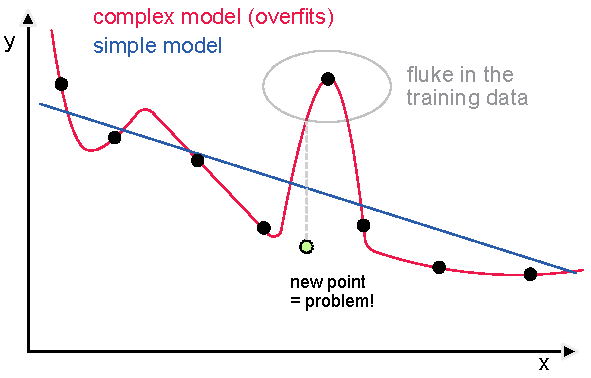
\includegraphics[width=0.7\linewidth]{files/overfitting-11a1b4147485a42b1df8dd6ae13058fb.pdf}
\caption[]{Illustration of overfitting: a model closely matching training data is rarely a good idea.}
\label{fig-overfit}
\end{figure}

A new point is added in light green. It is fair to say that it follows the general pattern of the other points. The simple model is not perfect and the error is non-negligible. Nevertheless, the error stemming from the complex model (shown with the dotted gray line) is approximately twice as large. This simplified example shows that models that are too close to the training data will catch idiosyncracies that will not occur in other datasets. A good model would overlook these idiosyncracies and stick to the enduring structure of the data.

\paragraph{The risk of overfitting: some solutions}

Obviously, the easiest way to avoid overfitting is to resist the temptation of complicated models (e.g., high-dimensional neural networks or tree ensembles).

The complexity of models is often proxied via two measures: the number of parameters of the model and their magnitude (often synthesized through their norm). These proxies are not perfect because some \textit{complex} models may only require a small number of parameters (or even small parameter values), but at least they are straightforward and easy to handle. There is no universal way of handling overfitting. Below, we detail a few tricks for some families of ML tools.

For \textbf{regressions}, there are two simple ways to deal with overfitting. The first is the number of parameters, that is, the number of predictors. Sometimes, it can be better to only select a subsample of features, especially if some of them are highly correlated (often, a threshold of 70\% is considered as too high for absolute correlations between features). The second solution is penalization (via LASSO, ridge or elasticnet), which helps reduce the magnitude of estimates and thus of the variance of predictions.

For tree-based methods, there are a variety of ways to reduce the risk of overfitting. When dealing with \textbf{simple trees}, the only way to proceed is to limit the number of leaves. This can be done in many ways. First, by imposing a maximum depth. If it is equal to $d$, then the tree can have at most $2^d$ terminal nodes. It is often advised not to go beyond $d=6$. The complexity parameter in \textit{rpart} (cp) is another way to shrink the size of trees: any new split must lead to a reduction in loss at least equal to cp. If not, the split is not deemed useful and is thus not performed. Thus when cp is large, the tree is not grown. The last two parameters available in \textit{rpart} are the minimum number of instances required in each leaf and the minimum number of instances per cluster requested in order to continue the splitting process. The higher (i.e., the more coercive) these figures are, the harder it is to grow complex trees.

In addition to these options, \textbf{random forests} allow to control for the number of trees in the forest. Theoretically (see \cite{breiman2001random}), this parameter is not supposed to impact the risk of overfitting because new trees only help reduce the total error via diversification. In practice, and for the sake of computation times, it is not recommended to go beyond 1,000 trees. Two other hyperparameters are the subsample size (on which each learner is trained) and the number of features retained for learning. They do not have a straightforward impact on bias and tradeoff, but rather on raw performace. For instance, if subsamples are too small, the trees will not learn enough. Same problem if the number of features is too low. On the other hand, choosing a large number of predictors (i.e., close to the total number) may lead to high correlations between each learner's prediction because the overlap in information contained in the training samples may be high.

\textbf{Boosted trees} have other options that can help alleviate the risk of overfitting. The most obvious one is the learning rate, which discounts the impact of each new tree by $\eta \in (0,1)$. When the learning rate is high, the algorithm learns too quickly and is prone to sticking close to the training data. When it's low, the model learns very progressively, which can be efficient if there are sufficiently many trees in the ensemble. Indeed, the learning rate and the number of trees must be chosen synchronously: if both are low, the ensemble will learn nothing and if both are large, it will overfit. The arsenal of boosted tree parameters does not stop there. The penalizations, both of score values and of the number of leaves, are naturally a tool to prevent the model from going too deep in the particularities of the training sample. Finally, constraints of monotonicity like those mentioned in Section~\ref{sec_boostext} are also an efficient way to impose some structure on the model and force it to detect particular patterns.

Lastly \textbf{neural networks} also have many options aimed at protecting them against overfitting. Just like for boosted trees, some of them are the learning rate and the penalization of weights and biases (via their norm). Constraints, like nonnegative constraints, can also help when the model theoretically requires positive inputs. Finally, dropout is always a direct way to reduce the dimension (number of parameters) of a network.

\subsubsection{The search for good hyperparameters}

\paragraph{Methods}

Let us assume that there are $p$ parameters to be defined before a model is run. The simplest way to proceed is to test different values of these parameters and choose the one that yields the best results. There are mainly two ways to perform these tests: independently and sequentially.

Independent tests are easy and come in two families: grid (deterministic) search and random exploration. The advantage of a deterministic approach is that it covers the space uniformly and makes sure that no corners are omitted. The drawback is the computation time. Indeed, for each parameter, it seems reasonable to test at least five values, which makes $5^p$ combinations. If $p$ is small (smaller than 3), this is manageable when the backtests are not too lengthy. When $p$ is large, the number of combinations may become prohibitive. This is when random exploration can be useful because in this case, the user specifies the number of tests upfront and the parameters are drawn randomly (usually uniformly over a given range for each parameter). The flaw in random search is that some areas in the parameter space may not be covered, which can be problematic if the best choice is located there. It is nonetheless shown in \cite{bergstra2012random} that random exploration is preferable to grid search.

Both grid and random searches are suboptimal because they are likely to spend time in zones of the parameter space that are irrelevant, thereby wasting computation time. Given a number of parameter points that have been tested, it is preferable to focus the search in areas where the best points are the most likely. This is possible via an interative process that adapts the search after each new point has been tested. In the large field of finance, a few papers dedicated to tuning are \cite{lee2020hyperparameter} and \cite{nystrup2020hyperparameter}.

One other popular approach in this direction is \textbf{Bayesian optimization} (BO). The central object is the objective function of the learning process. We call this function $O$ and it can be widely seen as a loss function possibly combined with penalization and constraints. For simplicity here, we will not mention the training/testing samples and they are considered to be fixed. The variable of interest is the vector $\textbf{p}=(p_1,\dots,p_l)$ which synthesizes the hyperparameters (learning rate, penalization intensities, number of models, etc.) that have an impact on $O$. The program we are interested in is

\begin{equation}
\label{eq-HPO}
\textbf{p}_*=\underset{\textbf{p}}{\text{argmin}} \ O(\textbf{p}).
\end{equation}

The main problem with this optimization is that the computation of $O(\textbf{p})$ is very costly. Therefore, it is critical to choose each trial for $\textbf{p}$ wisely. One key assumption of BO is that the distribution of $O$ is Gaussian and that $O$ can be proxied by a linear combination of the $p_l$. Said differently, the aim is to build a Bayesian linear regression between the input $\textbf{p}$ and the output (dependent variable) $O$. Once a model has been estimated, the information that is concentrated in the posterior density of $O$ is used to make an educated guess at where to look for new values of $\textbf{p}$.

This educated guess is made based on a so-called \textbf{acquisition function}. Suppose we have tested $m$ values for $\textbf{p}$, which we write $\textbf{p}^{(m)}$. The current best parameter is written $\textbf{p}_m^*=\underset{1\le k\le m}{\text{argmin}} \ O(\textbf{p}^{(k)})$. If we test a new point $\textbf{p}$, then it will lead to an improvement only if $O(\textbf{p})<O(\textbf{p}_m^*)$, that is if the new objective improves the minimum value that we already know. The average value of this improvement is

\begin{equation}
\label{eq-acquisition}
\textbf{EI}_m(\textbf{p})=\mathbb{E}_m[[O(\textbf{p}_m^*)-O(\textbf{p})]_+],
\end{equation}

where the positive part $[\cdot]_+$ emphasizes that when $O(\textbf{p})\ge O(\textbf{p}_m^*)$, the gain is zero. The expectation is indexed by $m$ because it is computed with respect to the posterior distribution of $O(\textbf{p})$ based on the $m$ samples $\textbf{p}^{(m)}$. The best choice for the next sample $\textbf{p}^{m+1}$ is then

\begin{equation}
\label{eq-EI}
\textbf{p}^{m+1}=\underset{\textbf{p}}{\text{argmax}} \ \textbf{EI}_m(\textbf{p}),
\end{equation}

which corresponds to the maximum location of the expected improvement. Instead of the EI, the optimization can be performed on other measures, like the probability of improvement, which is $\mathbb{P}_m[O(\textbf{p})<O(\textbf{p}_m^*)]$.

In compact form, the iterative process can be outlined as follows:

\begin{itemize}
\item \textbf{step 1}: compute $O(\textbf{p}^{(m)})$ for $m=1,\dots,M_0$ values of parameters.
\item \textbf{step 2a}: compute sequentially the posterior density of $O$ on all available points.
\item \textbf{step 2b}: compute the optimal new point to test $\textbf{p}^{(m+1)}$ given in Equation \ref{eq-EI}.
\item \textbf{step 2c}: compute the new objective value $O(\textbf{p}^{(m+1)})$.
\item \textbf{step 3}: repeat steps 2a to 2c as much as deemed reasonable and return the $\textbf{p}^{(m)}$ that yields the smallest objective value.
\end{itemize}

The interested reader can have a look at \cite{snoek2012practical} and \cite{frazier2018tutorial} for more details on the numerical facets of this method.

Finally, for the sake of completeness, we mention a last way to tune hyperparameters. Since the optimization scheme is $\underset{\textbf{p}}{\text{argmin}} \ O(\textbf{p})$, a natural way to proceed would be to use the sensitivity of $O$ with respect to $\textbf{p}$. Indeed, if the gradient $\frac{\partial O}{\partial p_l}$ is known, then a gradient descent will always improve the objective value. The problem is that it is hard to compute a reliable gradient (finite differences can become costly). Nonetheless, some methods (e.g., \cite{maclaurin2015gradient}) have been applied successfully to optimize over large dimensional parameter spaces.

We conclude by mentioning the survey \cite{bouthillier2020survey}, which spans 2 major AI conferences that took place in 2019. It shows that most papers resort to hyperparameter tuning. The two most often cited methods are \textit{manual tuning} (hand-picking) and \textit{grid search}.

\paragraph{Example: grid search}

In order to illustrate the process of grid search, we will try to find the best parameters for a boosted tree. We seek to quantify the impact of three parameters:

\begin{itemize}
\item \textbf{eta}, the learning rate,
\item \textbf{nrounds}, the number of trees that are grown,
\item \textbf{lambda}, the weight regularizer which penalizes the objective function through the total sum of squared weights/scores.
\end{itemize}

Below, we create a grid with the values we want to test for these parameters.

\begin{verbatim}
# Values for hyperparameters
eta_vals = [0.1, 0.3, 0.5, 0.7, 0.9]       # Values for eta
nrounds_vals = [10, 50, 100]               # Values for nrounds
lambda_vals = [0.01, 0.1, 1, 10, 100]      # Values for lambda

# Create all combinations
pars = list(product(eta_vals, nrounds_vals, lambda_vals))
print(f"Number of parameter combinations: {len(pars)}")
print("First few combinations:")
for p in pars[:6]:
    print(f"  eta={p[0]}, nrounds={p[1]}, lambda={p[2]}")
\end{verbatim}

\begin{verbatim}
Number of parameter combinations: 75
First few combinations:
  eta=0.1, nrounds=10, lambda=0.01
  eta=0.1, nrounds=10, lambda=0.1
  eta=0.1, nrounds=10, lambda=1
  eta=0.1, nrounds=10, lambda=10
  eta=0.1, nrounds=10, lambda=100
  eta=0.1, nrounds=50, lambda=0.01
\end{verbatim}

Given the computational cost of grid search, we perform the exploration on the dataset with the small number of features. We define a function that takes data and parameter inputs and returns an error metric for the algorithm. We choose the mean squared error to evaluate the impact of hyperparameter values.

\begin{verbatim}
def grid_par(train_matrix, test_features, test_label, eta, nrounds, lambda_val):
    """Train XGBoost with given parameters and return MSE."""
    params = {
        'eta': eta,
        'objective': 'reg:squarederror',
        'max_depth': 5,
        'lambda': lambda_val,
        'gamma': 0.1,
        'verbosity': 0
    }
    
    fit = xgb.train(
        params=params,
        dtrain=train_matrix,
        num_boost_round=nrounds
    )
    
    pred = fit.predict(test_features)
    return np.mean((pred - test_label) ** 2)  # Mean squared error
\end{verbatim}

\begin{verbatim}
# Prepare XGBoost matrices
train_matrix_xgb = xgb.DMatrix(
    data=training_sample[features_short].values,
    label=training_sample['R1M'].values
)
xgb_test = xgb.DMatrix(testing_sample[features_short].values)
test_label = testing_sample['R1M'].values

# Run grid search
results = []
for eta, nrounds, lambda_val in pars:
    error = grid_par(train_matrix_xgb, xgb_test, test_label, eta, nrounds, lambda_val)
    results.append({
        'eta': eta,
        'nrounds': nrounds,
        'lambda': lambda_val,
        'error': error
    })

# Convert to DataFrame
grd = pd.DataFrame(results)
print(grd.head(10))
\end{verbatim}

\begin{verbatim}
eta  nrounds  lambda     error
0  0.1       10    0.01  0.015553
1  0.1       10    0.10  0.015550
2  0.1       10    1.00  0.015550
3  0.1       10   10.00  0.015546
4  0.1       10  100.00  0.015546
5  0.1       50    0.01  0.015597
6  0.1       50    0.10  0.015617
7  0.1       50    1.00  0.015559
8  0.1       50   10.00  0.015568
9  0.1       50  100.00  0.015546
\end{verbatim}

Once the squared mean errors have been gathered, it is possible to plot them. We chose to work with 3 parameters on purpose because their influence can be simultaneuously plotted on one graph.

\begin{figure}[!htbp]
\centering
\begin{verbatim}
# Create faceted bar plot
grd['eta_str'] = grd['eta'].astype(str)

fig, axes = plt.subplots(len(nrounds_vals), len(lambda_vals), figsize=(14, 8), sharey=True)

for i, nr in enumerate(nrounds_vals):
    for j, lam in enumerate(lambda_vals):
        subset = grd[(grd['nrounds'] == nr) & (grd['lambda'] == lam)]
        ax = axes[i, j]
        bars = ax.bar(subset['eta_str'], subset['error'], color=sns.color_palette("husl", 5) )
        
        if i == 0:
            ax.set_title(f'lambda={lam}')
        if j == 0:
            ax.set_ylabel(f'nrounds={nr}')
        if i == len(nrounds_vals) - 1:
            ax.set_xlabel('eta')
        ax.tick_params(axis='x', labelsize=8)

plt.tight_layout()
plt.show()
\end{verbatim}
\caption[]{Plot of error metrics (MSEs) for many parameter values. Each row of graph corresponds to nrounds and each column to lambda.

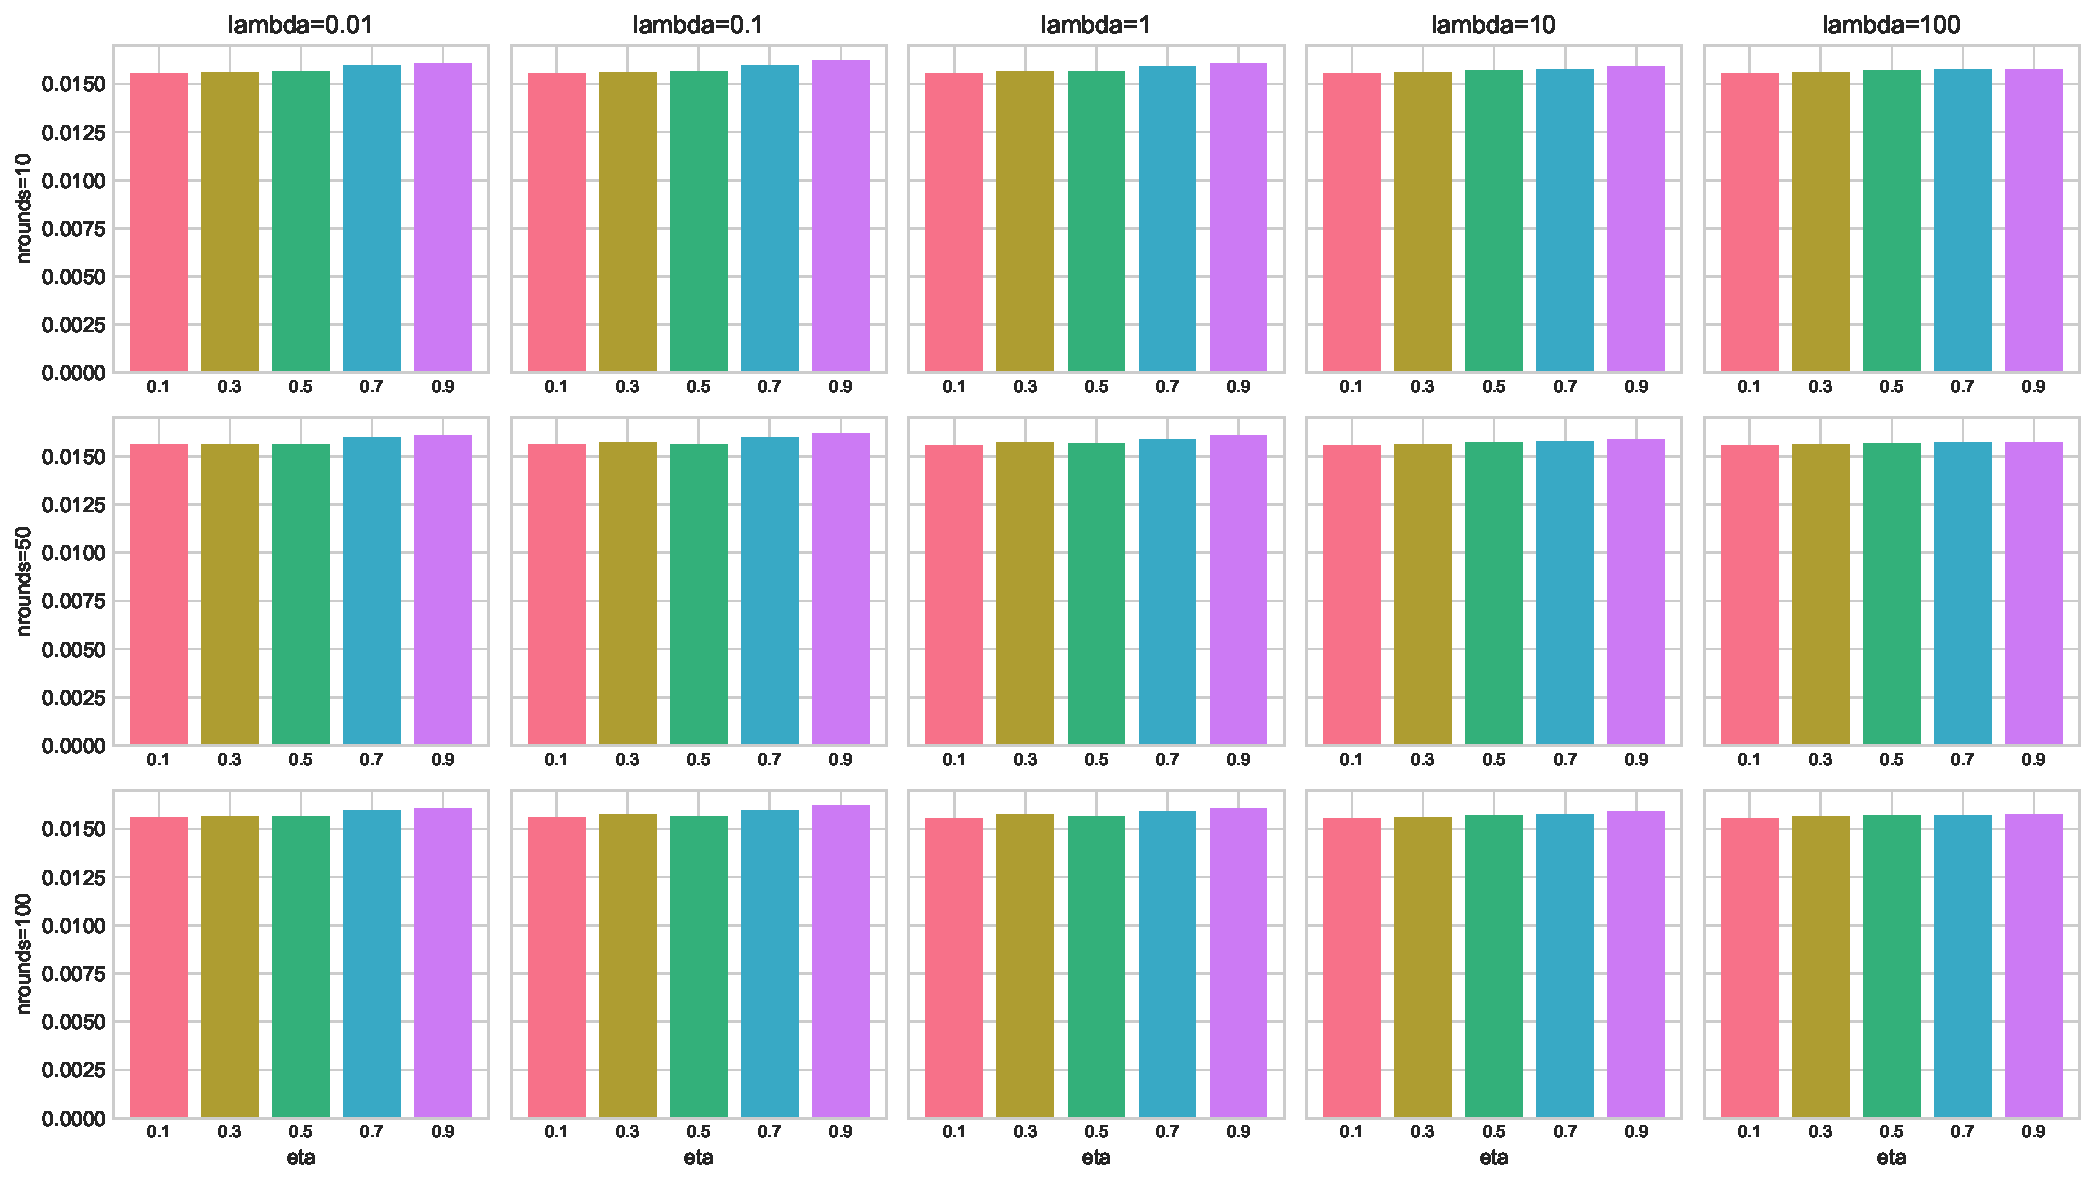
\includegraphics[width=0.7\linewidth]{files/2883468a9ebb8ca7f739050f6d48d9cc.pdf}}
\label{fig-gridvisu}
\end{figure}

In Figure~\ref{fig-gridvisu}, the main information is that a small learning rate ($\eta=0.1$) is detrimental to the quality of the forecasts when the number of trees is small (nrounds=10), which means that the algorithm does not learn enough.

Grid search can be performed in two stages: the first stage helps locate the zones that are of interest (with the lowest loss/objective values) and then zoom in on these zones with refined values for the parameter on the grid. With the results above, this would mean considering many learners (more than 50, possibly more than 100), and avoiding large learning rates such as $\eta=0.9$ or $\eta=0.8$.

\paragraph{Example: Bayesian optimization}

There are several packages in Python that relate to Bayesian optimization. We work with \textit{scikit-optimize}, which provides a general-purpose implementation.

\begin{verbatim}
from skopt import gp_minimize
from skopt.space import Real, Integer
from skopt.plots import plot_convergence

# Define the objective function (to minimize)
def bayes_objective(params):
    """Objective function for Bayesian optimization."""
    eta, lambda_val, nrounds = params
    
    xgb_params = {
        'eta': eta,
        'objective': 'reg:squarederror',
        'max_depth': 5,
        'lambda': lambda_val,
        'gamma': 0.1,
        'verbosity': 0
    }
    
    fit = xgb.train(
        params=xgb_params,
        dtrain=train_matrix_xgb,
        num_boost_round=int(nrounds)
    )
    
    pred = fit.predict(xgb_test)
    mse = np.mean((pred - test_label) ** 2)
    return mse  # Return MSE (to minimize)

# Define search space
search_space = [
    Real(0.2, 0.8, name='eta'),
    Real(0.1, 1.0, name='lambda'),
    Integer(10, 100, name='nrounds')
]

# Run Bayesian optimization
np.random.seed(42)
bayes_opt = gp_minimize(
    bayes_objective,
    search_space,
    n_calls=34,           # Total number of evaluations (10 initial + 24 iterations)
    n_initial_points=10,  # Number of initial random points
    acq_func='EI',        # Expected Improvement
    random_state=42,
    verbose=False
)

print("Best parameters found:")
print(f"  eta: {bayes_opt.x[0]:.4f}")
print(f"  lambda: {bayes_opt.x[1]:.4f}")
print(f"  nrounds: {bayes_opt.x[2]}")
print(f"  Best MSE: {bayes_opt.fun:.6f}")
\end{verbatim}

\begin{verbatim}
Best parameters found:
  eta: 0.3118
  lambda: 0.3520
  nrounds: 26
  Best MSE: 0.015575
\end{verbatim}

To confirm these results, we plot the relationship between the loss and hyperparameters. Each point corresponds to a value tested in the optimization.

\begin{figure}[!htbp]
\centering
\begin{verbatim}
# Extract history from optimization
history_df = pd.DataFrame({
    'eta': [x[0] for x in bayes_opt.x_iters],
    'lambda': [x[1] for x in bayes_opt.x_iters],
    'nrounds': [x[2] for x in bayes_opt.x_iters],
    'mse': bayes_opt.func_vals
})

fig, axes = plt.subplots(1, 2, figsize=(10, 4))

# Plot nrounds vs MSE
axes[0].scatter(history_df['nrounds'], history_df['mse'], alpha=0.7)
z = np.polyfit(history_df['nrounds'], history_df['mse'], 1)
p = np.poly1d(z)
x_line = np.linspace(history_df['nrounds'].min(), history_df['nrounds'].max(), 100)
axes[0].plot(x_line, p(x_line), 'r-', alpha=0.8, label='Linear fit')
axes[0].set_xlabel('nrounds')
axes[0].set_ylabel('MSE')
axes[0].legend()

# Plot lambda vs MSE
axes[1].scatter(history_df['lambda'], history_df['mse'], alpha=0.7)
z = np.polyfit(history_df['lambda'], history_df['mse'], 1)
p = np.poly1d(z)
x_line = np.linspace(history_df['lambda'].min(), history_df['lambda'].max(), 100)
axes[1].plot(x_line, p(x_line), 'r-', alpha=0.8, label='Linear fit')
axes[1].set_xlabel('lambda')
axes[1].set_ylabel('MSE')
axes[1].legend()

plt.tight_layout()
plt.show()
\end{verbatim}
\caption[]{Relationship between the loss (MSE) and hyperparameter values.

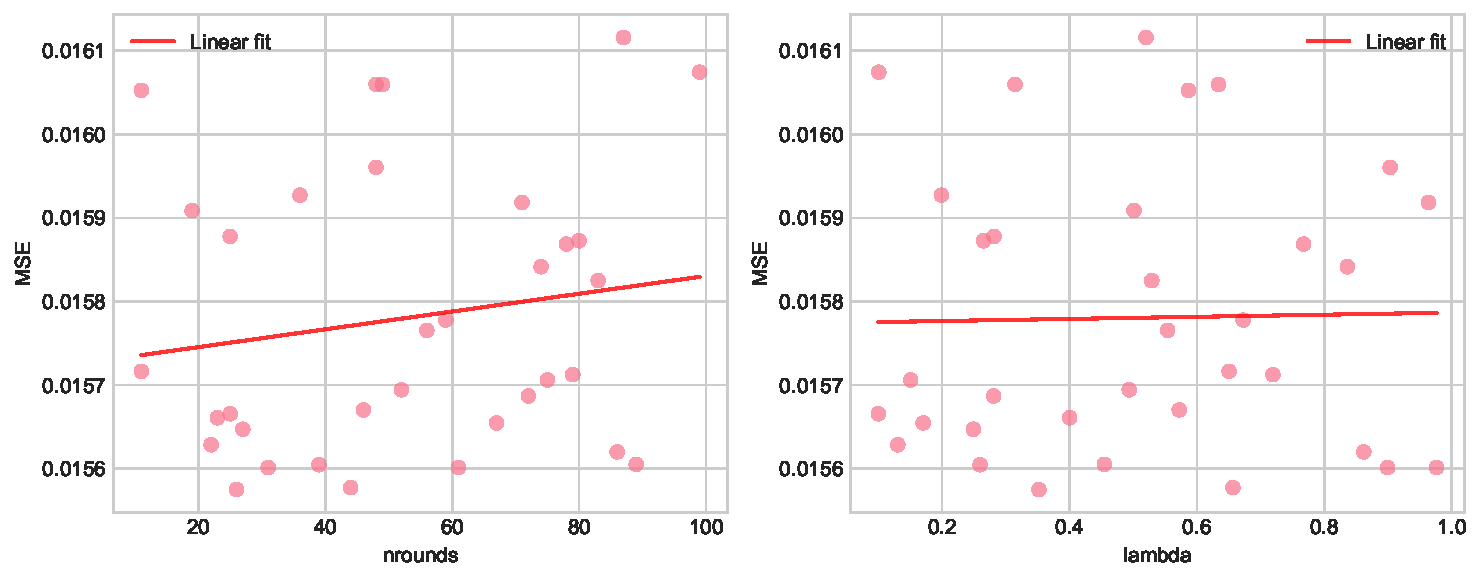
\includegraphics[width=0.7\linewidth]{files/27ea154e34f4c0befef57f33617c12d4.pdf}}
\label{fig-bayesoptfig}
\end{figure}

\subsubsection{Short discussion on validation in backtests}

The topic of validation in backtests is more complex than it seems. There are in fact two scales at which it can operate, depending on whether the forecasting model is dynamic (updated at each rebalancing) or fixed.

Let us start with the first option. In this case, the aim is to build a unique model and to test it on different time periods. There is an ongoing debate on the methods that are suitable to validate a model in that case. Usually, it makes sense to test the model on successive dates, moving forward posterior to the training. This is what makes more sense, as it replicates what would happen in a live situation.

In machine learning, a popular approach is to split the data into $K$ partitions and to test $K$ different models: each one is tested on one of the partitions but trained on the $K -1$ others. This so-called \textbf{cross-validation} (CV) is proscribed by most experts (and common sense) for a simple reason: most of the time, the training set encompasses data from future dates and tests on past values. Nonetheless, some advocate one particular form of CV that aims at making sure that there is no informational overlap between the training and testing set (Sections 7.4 and 12.4 in \cite{de2018advances}). The premise is that if the structure of the cross-section of returns is constant through time, then training on future points and testing on past data is not problematic as long as there is no overlap. The paper \cite{schnaubelt2019comparison} provides a comprehensive and exhaustive tour in many validation schemes.

One example cited in \cite{de2018advances} is the reaction to a model to an unseen crisis. Following the market crash of 2008, at least 11 years have followed without any major financial shake. One option to test the reaction of a recent model to a crash would be to train it on recent years (say 2015-2019) and test it on various points (e.g., months) in 2008 to see how it performs.

The advantage of a fixed model is that validation is easy: for one set of hyperparameters, test the model on a set of dates, and evaluate the performance of the model. Repeat the process for other parameters and choose the best alternative (or use Bayesian optimization).

The second major option is when the model is updated (retrained) at each rebalancing. The underlying idea here is that the structure of returns evolves through time and a dynamic model will capture the most recent trends. The drawback is that validation must (should?) be rerun at each rebalancing date.

Let us recall the dimensions of backtests:

\begin{itemize}
\item number of \textbf{strategies}: possibly dozens or hundreds, or even more;
\item number of trading \textbf{dates}: hundreds for monthly rebalancing;
\item number of \textbf{assets}: hundreds or thousands;
\item number of \textbf{features}: dozens or hundreds.
\end{itemize}

Even with a lot of computational power (GPUs, etc.), training many models over many dates is time-consuming, especially when it comes to hyperparameter tuning when the parameter space is large. Thus, validating models at each trading date of the out-of-sample period is not realistic.

One solution is to keep an early portion of the training data and to perform a smaller scale validation on this subsample. Hyperparameters are tested on a limited number of dates and most of the time, they exhibit stability: satisfactory parameters for one date are usually acceptable for the next one and the following one as well. Thus, the full backtest can be carried out with these values when updating the models at each period. The backtest nonetheless remains compute-intensive because the model has to be retrained with the most recent data for each rebalancing date.

\subsection{Ensemble models}

Let us be honest. When facing a prediction task, it is not obvious to determine the best choice between ML tools: penalized regressions, tree methods, neural networks, SVMs, etc. A natural and tempting alternative is to \textbf{combine} several algorithms (or the predictions that result from them) to try to extract value out of each engine (or learner). This intention is not new and contributions towards this goal go back at least to \cite{bates1969combination} (for the purpose of passenger flow forecasting).

Below, we outline a few books on the topic of ensembles. The latter have many names and synonyms, such as \textbf{forecast aggregation}, \textbf{model averaging}, \textbf{mixture of experts} or \textbf{prediction combination}. The first four references below are monographs, while the last two are compilations of contributions:

\begin{itemize}
\item \cite{zhou2012ensemble}: a very didactic book that covers the main ideas of ensembles;
\item \cite{schapire2012boosting}: the main reference for boosting (and hence, ensembling) with many theoretical results and thus strong mathematical groundings;
\item \cite{seni2010ensemble}: an introduction dedicated to tree methods mainly;
\item \cite{claeskens2008model}: an overview of model selection techniques with a few chapters focused on model averaging;
\item \cite{zhang2012ensemble}: a collection of thematic chapters on ensemble learning;
\item \cite{okun2011ensembles}: examples of applications of ensembles.
\end{itemize}

In this chapter, we cover the basic ideas and concepts behind the notion of ensembles. We refer to the above books for deeper treatments on the topic. We underline that several ensemble methods have already been mentioned and covered earlier, notably in Chapter \href{/chap-07-trees}{Tree-based methods}. Indeed, random forests and boosted trees are examples of ensembles. Hence, other early articles on the combination of learners are \cite{schapire1990strength}, \cite{jacobs1991adaptive} (for neural networks particularly), and \cite{freund1997decision}. Ensembles can for instance be used to aggregate models that are built on different datasets \citep{pesaran2011forecast}, and can be made time-dependent \citep{sun2020time}. For a theoretical view on ensembles, we refer to \cite{peng2022improvability} and \cite{razin2020drowning} (Bayesian perspective). Forecast combinations for returns are investigated in \cite{cheng2022stock} and widely reviewed by \cite{wang2022forecast} - see also \cite{scholz2022forecast} for a contrarian take (ensembles don't always work well). Finally, perspectives linked to asset pricing and factor modelling are provided in \cite{gospodinov2020generalized}, \cite{de2020subsampled} (subsampling and forecast aggregation) and \cite{remlinger2023expert} (Bernstein Online Aggregation).

From the standpoint of asset pricing anomalies, \cite{reschenhofer2024combining} discusses the combination of several factors: this allows to lower volatility.

\subsubsection{Linear ensembles}

\paragraph{Principles}

In this chapter we adopt the following notations. We work with $M$ models where $\tilde{y}_{i,m}$ is the prediction of model $m$ for instance $i$ and errors $\epsilon_{i,m}=y_i -\tilde{y}_{i,m}$ are stacked into a $(I\times M)$ matrix $\textbf{E}$. A linear combination of models has sample errors equal to $\textbf{Ew}$, where $\textbf{w}=w_m$ are the weights assigned to each model and we assume $\textbf{w}'\textbf{1}_M=1$. Minimizing the total (squared) error is thus a simple quadratic program with unique constraint. The Lagrange function is $L(\textbf{w})=\textbf{w}'\textbf{E}'\textbf{E}\textbf{w} -\lambda (\textbf{w}'\textbf{1}_M -1)$ and hence
\begin{equation}
\frac{\partial}{\partial \textbf{w}}L(\textbf{w})=\textbf{E}'\textbf{E}\textbf{w}-\lambda \textbf{1}_M=0 \quad \Leftrightarrow \quad \textbf{w}=\lambda(\textbf{E}'\textbf{E})^{-1}\textbf{1}_M,
\end{equation}

and the constraint imposes $\textbf{w}^*=\frac{(\textbf{E}'\textbf{E})^{ -1}\textbf{1}_M}{(\textbf{1}_M'\textbf{E}'\textbf{E})^{ -1}\textbf{1}_M}$. This form is similar to that of minimum variance portfolios.  If errors are unbiased ($\textbf{1}_I'\textbf{E}=\textbf{0}_M'$), then $\textbf{E}'\textbf{E}$ is the covariance matrix of errors.

This expression shows an important feature of optimized linear ensembles: they can only add value if the models tell different stories. If two models are redundant, $\textbf{E}'\textbf{E}$ will be close to singular and $\textbf{w}^*$ will arbitrage one against the other in a spurious fashion. This is the exact same problem as when mean-variance portfolios are constituted with highly correlated assets: in this case, diversification fails because when things go wrong, all assets go down. Another problem arises when the number of observations is too small compared to the number of assets so that the covariance matrix of returns is singular. This is not an issue for ensembles because the number of observations will usually be much larger than the number of models ($I>>M$).

In the limit when correlations increase to one, the above formulation becomes highly unstable and ensembles cannot be trusted. One heuristic way to see this is when $M=2$ and
\begin{equation}
\textbf{E}'\textbf{E}=\left[
\begin{array}{cc} \sigma_1^2 & \rho\sigma_1\sigma_2 \\
\rho\sigma_1\sigma_2 & \sigma_2^2 \\
\end{array}
\right] \quad \Leftrightarrow  \quad 
(\textbf{E}'\textbf{E})^{-1}=\frac{1}{1-\rho^2}\left[
\begin{array}{cc} \sigma_1^{-2} & -\rho(\sigma_1\sigma_2)^{-1} \\
-\rho(\sigma_1\sigma_2)^{-1} & \sigma_2^{-2} \\
\end{array}
\right]
\end{equation}

so that when $\rho \rightarrow 1$, the model with the smallest errors (minimum $\sigma_i^2$) will see its weight increasing towards infinity while the other model will have a similarly large \textbf{negative weight}: the model arbitrages between two highly correlated variables. This seems like a very bad idea.

There is another illustration of the issues caused by correlations. Let's assume we face $M$ correlated errors $\epsilon_m$ with pairwise correlation $\rho$, zero mean and variance $\sigma^2$. The variance of errors is
\begin{align*}
\mathbb{E}\left[\frac{1}{M}\sum_{m=1}^M \epsilon_m^2 \right]&=\frac{1}{M^2}\left[\sum_{m=1}^M\epsilon_m^2+\sum_{m\neq n}\epsilon_n\epsilon_m\right] \\
&=\frac{\sigma^2}{M}+\frac{1}{M^2}\sum_{n\neq m} \rho \sigma^2 \\
& =\rho \sigma^2 +\frac{\sigma^2(1-\rho)}{M}
\end{align*}
where while the second term converges to zero as $M$ increases, the first term remains and is \textbf{linearly increasing} with $\rho$. In passing, because variances are always positive, this result implies that the common pairwise correlation between $M$ variables is bounded below by $-(M -1)^{ -1}$. This result is interesting but rarely found in textbooks.

One improvement proposed to circumvent the trouble caused by correlations, advocated in a seminal publication \citep{breiman1996stacked}, is to enforce positivity constraints on the weights and solve

\begin{equation}
\underset{\textbf{w}}{\text{argmin}} \ \textbf{w}'\textbf{E}'\textbf{E}\textbf{w} , \quad \text{s.t.} \quad \left\{ 
\begin{array}{l} \textbf{w}'\textbf{1}_M=1 \\ w_m \ge 0 \quad \forall m \end{array}\right. .
\end{equation}

Mechanically, if several models are highly correlated, the constraint will impose that only one of them will have a nonzero weight. If there are many models, then just a few of them will be selected by the minimization program. In the context of portfolio optimization, \cite{jagannathan2003risk} have shown the counter-intuitive benefits of constraints in the construction of mean-variance allocations. In our setting, the constraint will similarly help discriminate wisely among the `best' models.

In the literature, forecast combination and model averaging (which are synonyms of ensembles) have been tested on stock markets as early as in \cite{von1972probabilistic}. Surprisingly, the articles were not published in Finance journals but rather in fields such as Management (\cite{virtanen1987forecasting}, \cite{wang2012stock}), Economics and Econometrics (\cite{donaldson1996forecast}, \cite{clark2009improving}, \cite{mascio2020market}), Operations Research (\cite{huang2005forecasting}, \cite{leung2001using}, and \cite{bonaccolto2019developing}), and Computer Science (\cite{harrald1997evolving}, \cite{hassan2007fusion}).

In the general forecasting literature, many alternative (refined) methods for combining forecasts have been studied. Trimmed opinion pools \citep{grushka2016ensembles} compute averages over the predictions that are not too extreme (or not too noisy, see \cite{chiang2021modeling}). Ensembles with weights that depend on previous past errors are developed in \cite{pike2020combining}. We refer to \cite{gaba2017combining} for a more exhaustive list of combinations as well as for an empirical study of their respective efficiency. Finally, for a theoretical discussion on model averaging versus model selection, we point to \cite{pengimprovability}.
Overall, findings are mixed and the heuristic simple average is, as usual, hard to beat (see, e.g., \cite{genre2013combining}).

\paragraph{Example}

In order to build an ensemble, we must gather the predictions and the corresponding errors into the $\textbf{E}$ matrix. We will work with 5 models that were trained in the previous chapters: penalized regression, simple tree, random forest, xgboost and feed-forward neural network. The training errors have zero means, hence $\textbf{E}'\textbf{E}$ is the covariance matrix of errors between models.

\begin{verbatim}
import numpy as np
import pandas as pd
import matplotlib.pyplot as plt
import warnings
warnings.filterwarnings('ignore')
plt.style.use('seaborn-v0_8-whitegrid')

import os
os.environ["KERAS_BACKEND"] = "jax"

import keras
from keras import layers
from sklearn.linear_model import ElasticNet
from sklearn.tree import DecisionTreeRegressor
from sklearn.ensemble import RandomForestRegressor
import xgboost as xgb
from scipy.optimize import minimize
import pandas_datareader.data as web
from datetime import datetime

from data_build import generate_data
data_ml, features, features_short, returns, stock_ids, stock_ids_short = generate_data()
features_short = ["Div_yld", "EPS", "size_avg_252d", "mom_252", "OCF_Growth_1Y", "PB", "vol_252"]
separation_date = "2017-01-15"

# Data preparation
data_ml_clean = data_ml.dropna()
training_sample = data_ml_clean[data_ml['date'] <= separation_date]
testing_sample = data_ml_clean[data_ml['date'] > separation_date]
\end{verbatim}

\begin{verbatim}
# Train models from previous chapters
# 1. Penalized regression
x_penalized_train = training_sample[features].values
y_train = training_sample['R1M'].values
fit_pen_pred = ElasticNet(alpha=0.1, l1_ratio=0.1, fit_intercept=True)
fit_pen_pred.fit(x_penalized_train, y_train)

# 2. Simple tree
fit_tree = DecisionTreeRegressor(
    min_samples_leaf=1500,
    min_samples_split=4000,
    ccp_alpha=0.0001,
    max_depth=5
)
fit_tree.fit(training_sample[features], y_train)

# 3. Random forest
np.random.seed(42)
fit_RF = RandomForestRegressor(
    n_estimators=40,
    max_samples=10000,
    bootstrap=True,
    min_samples_leaf=250,
    max_features=30,
    random_state=42
)
fit_RF.fit(training_sample[features], y_train)

# 4. XGBoost (on extreme values)
q20 = training_sample['R1M'].quantile(0.2)
q80 = training_sample['R1M'].quantile(0.8)
train_extreme = training_sample[
    (training_sample['R1M'] < q20) | (training_sample['R1M'] > q80)
]
train_features_xgb = train_extreme[features].values
train_label_xgb = train_extreme['R1M'].values
train_matrix_xgb = xgb.DMatrix(data=train_features_xgb, label=train_label_xgb)
params_xgb = {
    'eta': 0.4,
    'objective': 'reg:squarederror',
    'max_depth': 4,
    'verbosity': 0
}
fit_xgb = xgb.train(params=params_xgb, dtrain=train_matrix_xgb, num_boost_round=18)

# 5. Neural network
NN_train_features = training_sample[features].values
NN_train_labels = training_sample['R1M'].values
model = keras.Sequential([
    layers.Dense(units=16, activation='relu', input_shape=(NN_train_features.shape[1],)),
    layers.Dense(units=8, activation='tanh'),
    layers.Dense(units=1)
])
model.compile(loss='mean_squared_error', optimizer='rmsprop', metrics=['mean_absolute_error'])
model.fit(NN_train_features, NN_train_labels, epochs=10, batch_size=512, verbose=0)
\end{verbatim}

\begin{verbatim}
<keras.src.callbacks.history.History at 0x124a30cd0>
\end{verbatim}

\begin{verbatim}
# Compute training errors for each model
x_penalized_test = testing_sample[features].values
xgb_test = xgb.DMatrix(testing_sample[features].values)
NN_test_features = testing_sample[features].values

err_pen_train = fit_pen_pred.predict(x_penalized_train) - training_sample['R1M'].values      # Reg.
err_tree_train = fit_tree.predict(training_sample[features]) - training_sample['R1M'].values # Tree
err_RF_train = fit_RF.predict(training_sample[features]) - training_sample['R1M'].values     # RF
err_XGB_train = fit_xgb.predict(xgb.DMatrix(training_sample[features].values)) - training_sample['R1M'].values  # XGBoost
err_NN_train = model.predict(NN_train_features, verbose=0).flatten() - training_sample['R1M'].values  # NN

# E matrix
E = np.column_stack([err_pen_train, err_tree_train, err_RF_train, err_XGB_train, err_NN_train])
col_names = ["Pen_reg", "Tree", "RF", "XGB", "NN"]

# Correlation matrix
E_df = pd.DataFrame(E, columns=col_names)
print("Correlation matrix of training errors:")
print(E_df.corr().round(3))
\end{verbatim}

\begin{verbatim}
Correlation matrix of training errors:
         Pen_reg   Tree     RF    XGB     NN
Pen_reg    1.000  0.264  0.898  0.192  0.319
Tree       0.264  1.000  0.328  0.047  0.143
RF         0.898  0.328  1.000  0.031  0.327
XGB        0.192  0.047  0.031  1.000  0.031
NN         0.319  0.143  0.327  0.031  1.000
\end{verbatim}

As is shown by the correlation matrix, the models fail to generate heterogeneity in their predictions. The minimum correlation (though above 95\%!) is obtained by the boosted tree models. Below, we compare the training accuracy of models by computing the average absolute value of errors.

\begin{verbatim}
# Mean absolute error for columns of E
print("Mean absolute error by model:")
print(pd.Series(np.abs(E).mean(axis=0), index=col_names).round(5))
\end{verbatim}

\begin{verbatim}
Mean absolute error by model:
Pen_reg    0.07472
Tree       0.02103
RF         0.03272
XGB        0.03554
NN         0.02543
dtype: float64
\end{verbatim}

The best performing ML engine is the random forest. The boosted tree model is the worst, by far. Below, we compute the optimal (non-constrained) weights for the combination of models.

\begin{verbatim}
# Optimal weights
ones = np.ones(5)
EtE = E.T @ E
EtE_inv = np.linalg.inv(EtE)
w_ensemble = EtE_inv @ ones
w_ensemble = w_ensemble / w_ensemble.sum()
print("Optimal unconstrained weights:")
print(pd.Series(w_ensemble.round(3), index=col_names))
\end{verbatim}

\begin{verbatim}
Optimal unconstrained weights:
Pen_reg   -0.114
Tree       0.169
RF         0.140
XGB        0.260
NN         0.545
dtype: float64
\end{verbatim}

Because of the high correlations, the optimal weights are not balanced and diversified: they load heavily on the random forest learner (best in sample model) and `short' a few models in order to compensate. As one could expect, the model with the largest negative weights (Pen\_reg) has a very high correlation with the random forest algorithm (0.997).

Note that the weights are of course computed with \textbf{training errors}. The optimal combination is then tested on the testing sample. Below, we compute out-of-sample (testing) errors and their average absolute value.

\begin{verbatim}
# Testing errors
err_pen_test = fit_pen_pred.predict(x_penalized_test) - testing_sample['R1M'].values      # Reg.
err_tree_test = fit_tree.predict(testing_sample[features]) - testing_sample['R1M'].values  # Tree
err_RF_test = fit_RF.predict(testing_sample[features]) - testing_sample['R1M'].values      # RF
err_XGB_test = fit_xgb.predict(xgb_test) - testing_sample['R1M'].values                    # XGBoost
err_NN_test = model.predict(NN_test_features, verbose=0).flatten() - testing_sample['R1M'].values  # NN

# E_test matrix
E_test = np.column_stack([err_pen_test, err_tree_test, err_RF_test, err_XGB_test, err_NN_test])
E_test_df = pd.DataFrame(E_test, columns=col_names)

# Mean absolute error for testing
print("Mean absolute error by model (testing):")
print(pd.Series(np.abs(E_test).mean(axis=0), index=col_names).round(5))
\end{verbatim}

\begin{verbatim}
Mean absolute error by model (testing):
Pen_reg    0.08322
Tree       0.02214
RF         0.03742
XGB        0.03345
NN         0.02501
dtype: float64
\end{verbatim}

The boosted tree model is still the worst performing algorithm while the simple models (regression and simple tree) are the ones that fare the best. The most naive combination is the simple average of model and predictions.

\begin{verbatim}
# Equally weighted combination
err_EW_test = E_test.mean(axis=1)
print(f"Mean absolute error (EW combination): {np.abs(err_EW_test).mean():.5f}")
\end{verbatim}

\begin{verbatim}
Mean absolute error (EW combination): 0.02839
\end{verbatim}

Because the errors are very correlated, the equally weighted combination of forecasts yields an average error which lies `in the middle' of individual errors. The diversification benefits are too small. Let us now test the `optimal' combination $\textbf{w}^*=\frac{(\textbf{E}'\textbf{E})^{ -1}\textbf{1}_M}{(\textbf{1}_M'\textbf{E}'\textbf{E})^{ -1}\textbf{1}_M}$.

\begin{verbatim}
# Optimal unconstrained combination
err_opt_test = E_test @ w_ensemble
print(f"Mean absolute error (optimal combination): {np.abs(err_opt_test).mean():.5f}")
\end{verbatim}

\begin{verbatim}
Mean absolute error (optimal combination): 0.01079
\end{verbatim}

Again, the result is disappointing because of the lack of diversification across models. The correlations between errors are high not only on the training sample, but also on the testing sample, as shown below.

\begin{verbatim}
# Correlation matrix of testing errors
print("Correlation matrix of testing errors:")
print(E_test_df.corr().round(3))
\end{verbatim}

\begin{verbatim}
Correlation matrix of testing errors:
         Pen_reg   Tree     RF    XGB     NN
Pen_reg    1.000  0.265  0.909  0.159  0.321
Tree       0.265  1.000  0.326  0.042  0.127
RF         0.909  0.326  1.000  0.030  0.324
XGB        0.159  0.042  0.030  1.000  0.052
NN         0.321  0.127  0.324  0.052  1.000
\end{verbatim}

The leverage from the optimal solution only exacerbates the problem and underperforms the heuristic uniform combination. We end this section with the constrained formulation of \cite{breiman1996stacked} using quadratic programming. If we write $\mathbf{\Sigma}$ for the covariance matrix of errors, we seek
\begin{equation}
\mathbf{w}^*=\underset{\mathbf{w}}{\text{argmin}} \ \mathbf{w}'\mathbf{\Sigma}\mathbf{w}, \quad \mathbf{1}'\mathbf{w}=1, \quad w_i\ge 0,
\end{equation}
The constraints will be handled as:

\begin{equation}
\mathbf{A} \mathbf{w}= \begin{bmatrix} 
1 & 1 & 1 \\
1 & 0 & 0\\
0 & 1 & 0 \\
0 & 0 & 1
\end{bmatrix} \mathbf{w} \hspace{9mm} \text{ compared to} \hspace{9mm} \mathbf{b}=\begin{bmatrix} 1 \\ 0 \\ 0 \\ 0 \end{bmatrix},
\end{equation}

where the first line will be an equality (weights sum to one) and the last three will be inequalities (weights are all positive).

\begin{verbatim}
from scipy.optimize import minimize

Sigma = E.T @ E                         # Unscaled covariance matrix
nb_mods = Sigma.shape[0]                # Number of models

# Objective function: w' Sigma w
def objective(w):
    return w @ Sigma @ w

# Constraints
constraints = [
    {'type': 'eq', 'fun': lambda w: np.sum(w) - 1}  # Weights sum to 1
]

# Bounds: all weights >= 0
bounds = [(0, None) for _ in range(nb_mods)]

# Initial guess
w0 = np.ones(nb_mods) / nb_mods

# Solve
result = minimize(objective, w0, method='SLSQP', bounds=bounds, constraints=constraints)
w_const = result.x

print("Constrained optimal weights:")
print(pd.Series(w_const.round(3), index=col_names))
\end{verbatim}

\begin{verbatim}
Constrained optimal weights:
Pen_reg    0.000
Tree       0.202
RF         0.000
XGB        0.244
NN         0.554
dtype: float64
\end{verbatim}

Compared to the unconstrained solution, the weights are sparse and concentrated in one or two models, usually those with small training sample errors.

\subsubsection{Stacked ensembles}

\paragraph{Two-stage training}

\textbf{Stacked ensembles} are a natural generalization of linear ensembles. The idea of generalizing linear ensembles goes back at least to \cite{wolpert1992stacked}. In the general case, the training is performed in two stages. The first stage is the simple one, whereby the $M$ models are trained independently, yielding the predictions $\tilde{y}_{i,m}$ for instance $i$ and model $m$. The second step is to consider the output of the trained models as input for a new level of machine learning optimization. The second level predictions are $\breve{y}_i=h(\tilde{y}_{i,1},\dots,\tilde{y}_{i,M})$, where $h$ is a new learner (see Figure below). Linear ensembles are of course stacked ensembles in which the second layer is a linear regression.

The same techniques are then applied to minimize the error between the true values $y_i$ and the predicted ones $\breve{y}_i$.

\begin{figure}[!htbp]
\centering
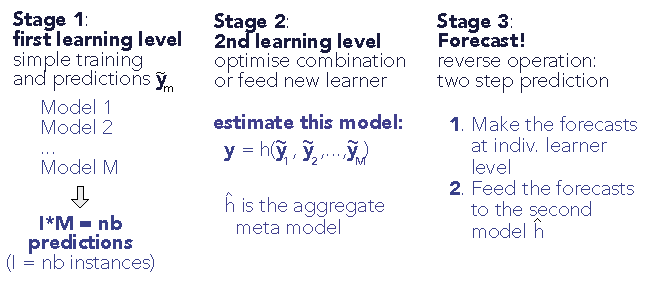
\includegraphics[width=0.7\linewidth]{files/stack-3e9ffe3958276cc8c46568c50b93cdb8.pdf}
\caption[]{Scheme of stacked ensembles.}
\label{fig-stackscheme}
\end{figure}

\paragraph{Code and results}

Below, we create a low-dimensional neural network which takes in the individual predictions of each model and compiles them into a synthetic forecast.

\begin{verbatim}
# Define the stacked neural network
model_stack = keras.Sequential([
    layers.Dense(units=8, activation='relu', input_shape=(nb_mods,)),
    layers.Dense(units=4, activation='tanh'),
    layers.Dense(units=1)
])
\end{verbatim}

The configuration is very simple. We do not include any optional arguments and hence the model is likely to overfit. As we seek to predict returns, the loss function is the standard $L^2$ norm.

\begin{verbatim}
# Model specification
model_stack.compile(
    loss='mean_squared_error',
    optimizer='rmsprop',
    metrics=['mean_absolute_error']
)
model_stack.summary()
\end{verbatim}

\begin{verbatim}
Model: "sequential_1"
\end{verbatim}

\begin{verbatim}
+---------------------------------+------------------------+---------------+
| Layer (type)                    | Output Shape           |       Param # |
+---------------------------------+------------------------+---------------+
| dense_3 (Dense)                 | (None, 8)              |            48 |
+---------------------------------+------------------------+---------------+
| dense_4 (Dense)                 | (None, 4)              |            36 |
+---------------------------------+------------------------+---------------+
| dense_5 (Dense)                 | (None, 1)              |             5 |
+---------------------------------+------------------------+---------------+
\end{verbatim}

\begin{verbatim}
Total params: 89 (356.00 B)
\end{verbatim}

\begin{verbatim}
Trainable params: 89 (356.00 B)
\end{verbatim}

\begin{verbatim}
Non -trainable params: 0 (0.00 B)
\end{verbatim}

\begin{figure}[!htbp]
\centering
\begin{verbatim}
# Prepare predictions as features
y_tilde = E + np.tile(training_sample['R1M'].values.reshape(-1, 1), nb_mods)     # Train preds
y_test_stack = E_test + np.tile(testing_sample['R1M'].values.reshape(-1, 1), nb_mods)  # Testing

# Train the stacked model
fit_NN_stack = model_stack.fit(
    y_tilde, training_sample['R1M'].values,    # Train features & labels
    epochs=12, batch_size=512, verbose=0,       # Train parameters (quiet: keeps the
                                                # figure caption free of the training log)
    validation_data=(y_test_stack, testing_sample['R1M'].values)  # Validation
)

# Plot training history
fig, axes = plt.subplots(1, 2, figsize=(12, 4))
axes[0].plot(fit_NN_stack.history['loss'], label='Training')
axes[0].plot(fit_NN_stack.history['val_loss'], label='Validation')
axes[0].set_xlabel('Epoch'); axes[0].set_ylabel('Loss'); axes[0].legend()
axes[1].plot(fit_NN_stack.history['mean_absolute_error'], label='Training')
axes[1].plot(fit_NN_stack.history['val_mean_absolute_error'], label='Validation')
axes[1].set_xlabel('Epoch'); axes[1].set_ylabel('MAE'); axes[1].legend()
plt.tight_layout(); plt.show()
\end{verbatim}
\caption[]{Training metrics for the ensemble model.

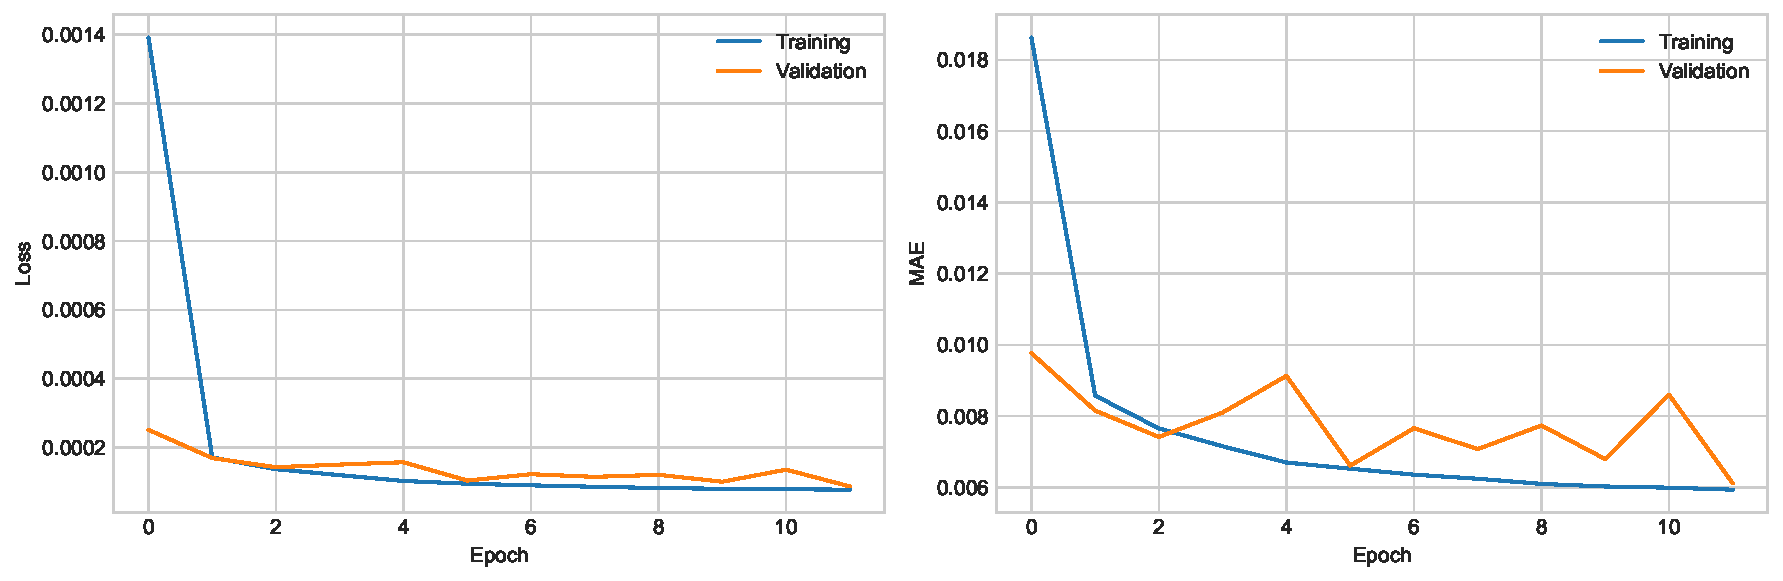
\includegraphics[width=0.7\linewidth]{files/bbe0eec3f90c29f829d7fbdcff102fac.pdf}}
\label{fig-stackNN2}
\end{figure}

The performance of the ensemble is again disappointing: the learning curve is flat in the figure above, hence the rounds of back-propagation are useless. The training adds little value which means that the new overarching layer of ML does not enhance the original predictions. Again, this is because all ML engines seem to be capturing the same patterns and both their linear and non-linear combinations fail to improve their performance.

\subsubsection{Extensions}

\paragraph{Exogenous variables}

In a financial context, macro-economic indicators could add value to the process. It is possible that some models perform better under certain conditions and exogenous predictors can help introduce a flavor of \textbf{economic-driven conditionality} in the predictions.

Adding macro-variables to the set of predictors (here, predictions) $\tilde{y}_{i,m}$ could seem like one way to achieve this. However, this would amount to mix predicted values with (possibly scaled) economic indicators and that would not make much sense.

One alternative outside the perimeter of ensembles is to train simple trees on a set of macro-economic indicators. If the labels are the (possibly absolute) errors stemming from the original predictions, then the trees will create clusters of homogeneous error values. This will hint towards which conditions lead to the best and worst forecasts.
We test this idea below, using aggregate data from the Federal Reserve of Saint Louis. A simple downloading function is available via pandas-datareader. We download and format the data in the next chunk. CPIAUCSL is a code for consumer price index and T10Y2YM is a code for the term spread (10Y minus 2Y).

\begin{verbatim}
# Download FRED data
start_date = datetime(2000, 1, 1)
end_date = datetime(2020, 12, 31)

cpi = web.DataReader('CPIAUCSL', 'fred', start_date, end_date)
ts = web.DataReader('T10Y2YM', 'fred', start_date, end_date)

# Compute inflation
cpi['inflation'] = cpi['CPIAUCSL'].pct_change()
ts.columns = ['termspread']

# Create ensemble data with macro variables
ens_data = testing_sample[['date']].copy()
ens_data['err_NN_test'] = err_NN_test
ens_data['month_start'] = pd.to_datetime(ens_data['date']).dt.to_period('M').dt.to_timestamp()

# Merge with macro data
cpi_monthly = cpi[['inflation']].reset_index()
cpi_monthly.columns = ['month_start', 'inflation']
ts_monthly = ts.reset_index()
ts_monthly.columns = ['month_start', 'termspread']

ens_data = ens_data.merge(cpi_monthly, on='month_start', how='left')
ens_data = ens_data.merge(ts_monthly, on='month_start', how='left')

print(ens_data.head())
\end{verbatim}

\begin{verbatim}
date  err_NN_test month_start  inflation  termspread
0 2017-01-31    -0.005671  2017-01-01   0.004043        1.22
1 2017-02-28    -0.015538  2017-02-01   0.001593        1.22
2 2017-03-31    -0.012140  2017-03-01  -0.000467        1.17
3 2017-04-30    -0.016495  2017-04-01   0.001234        1.06
4 2017-05-31    -0.020685  2017-05-01  -0.000774        1.00
\end{verbatim}

We can now build a tree that tries to explain the accuracy of models as a function of macro-variables.

\begin{figure}[!htbp]
\centering
\begin{verbatim}
from sklearn.tree import DecisionTreeRegressor, plot_tree

# Prepare data for tree
ens_data_clean = ens_data.dropna(subset=['inflation', 'termspread'])
X_macro = ens_data_clean[['inflation', 'termspread']]
y_macro = np.abs(ens_data_clean['err_NN_test'])

# Fit tree
fit_ens = DecisionTreeRegressor(ccp_alpha=0.001, max_depth=3)
fit_ens.fit(X_macro, y_macro)

# Plot tree
plt.figure(figsize=(12, 8))
plot_tree(fit_ens, feature_names=['inflation', 'termspread'], filled=True, rounded=True)
plt.tight_layout()
plt.show()
\end{verbatim}
\caption[]{Conditional performance of a ML engine.

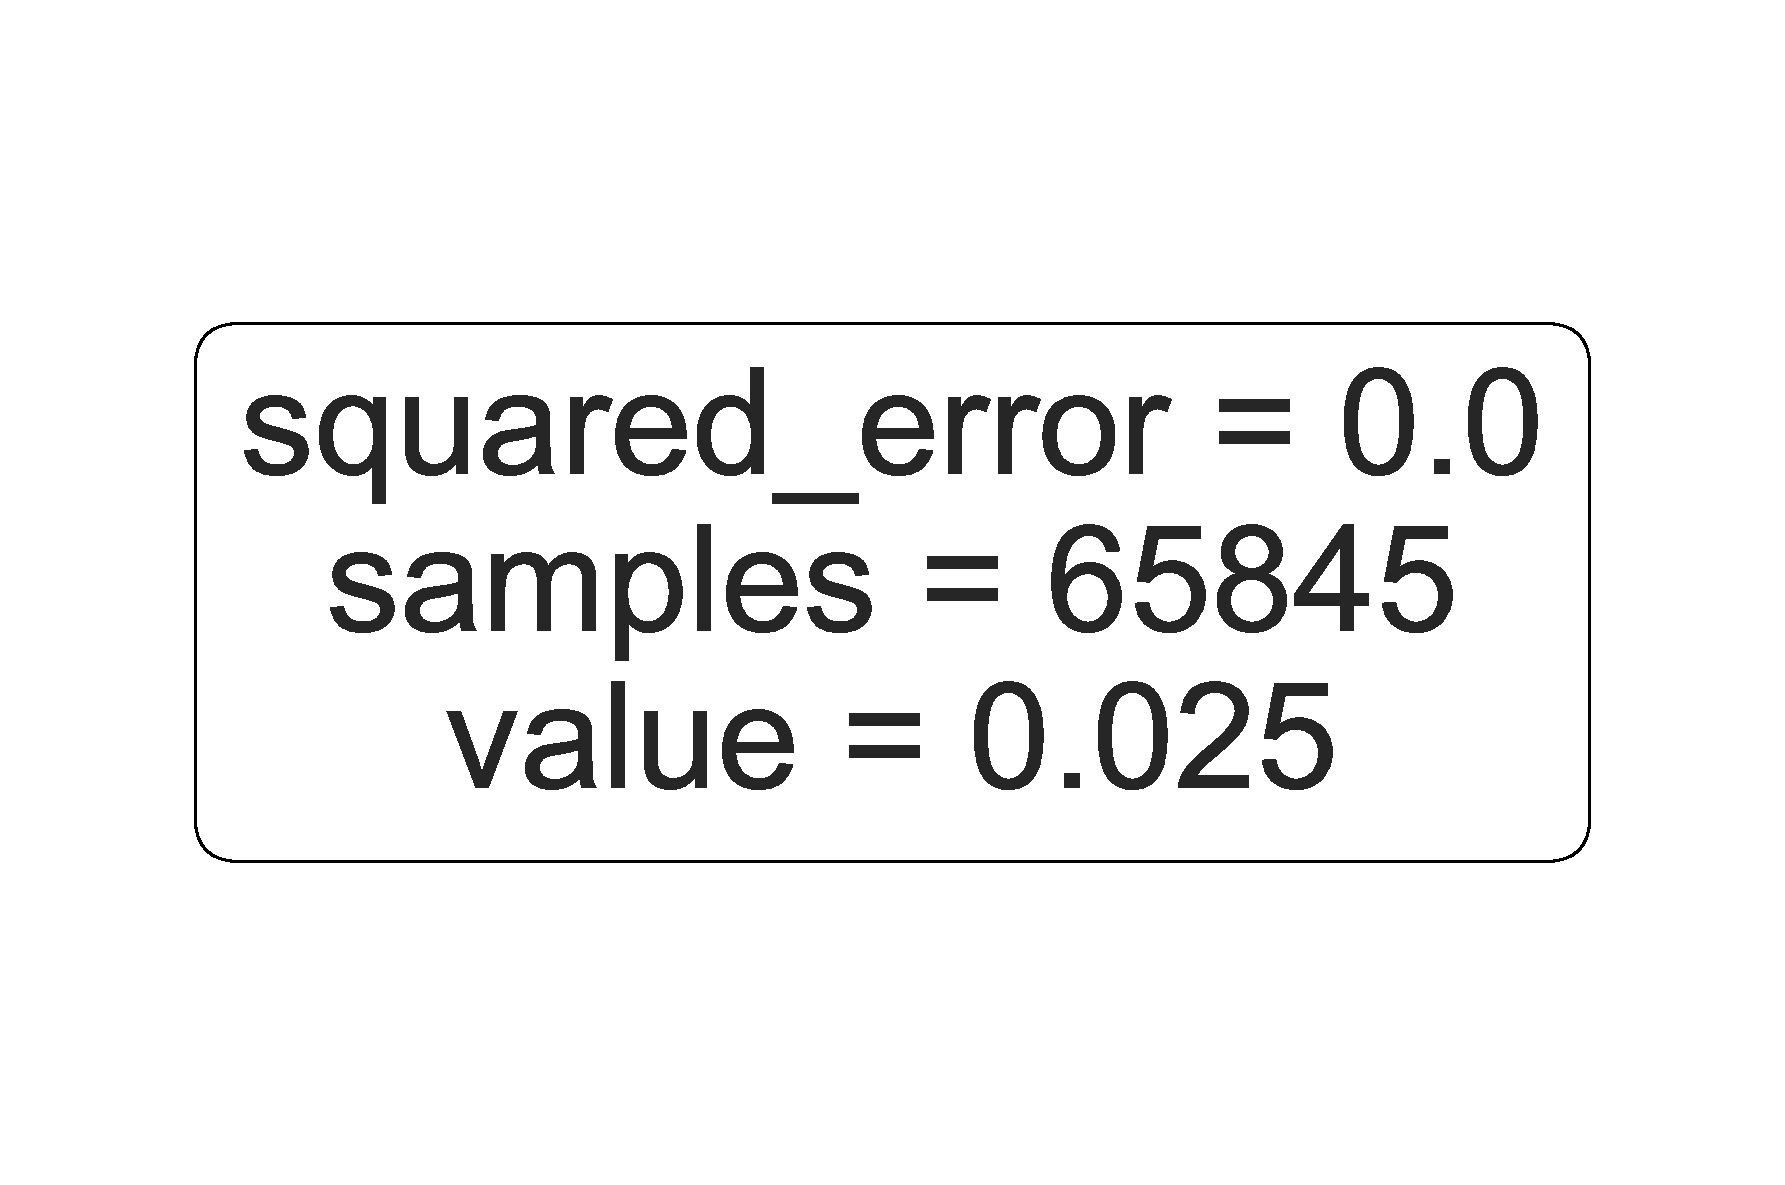
\includegraphics[width=0.7\linewidth]{files/5f1aeb77891bea391258f63de00844fe.pdf}}
\label{fig-ensfred2}
\end{figure}

The tree creates clusters which have homogeneous values of absolute errors. One big cluster gathers 92\% of predictions (the left one) and is the one with the smallest average. It corresponds to the periods when the term spread is above 0.29 (in percentage points). The other two groups (when the term spread is below 0.29\%) are determined according to the level of inflation. If the latter is positive, then the average absolute error is 7\%, if not, it is 12\%. This last number, the highest of the three clusters, indicates that when the term spread is low and the inflation negative, the model's predictions are not trustworthy because their errors have a magnitude twice as large as in other periods. Under these circumstances (which seem to be linked to a dire economic environment), it may be wiser not to use ML-based forecasts.

\paragraph{Shrinking inter-model correlations}

As shown earlier in this chapter, one major problem with ensembles arises when the first layer of predictions is highly correlated. In this case, ensembles are pretty much useless. There are several tricks that can help reduce this correlation, but the simplest and best is probably to alter training samples. If algorithms do not see the same data, they will probably infer different patterns.

There are several ways to split the training data so as to build different subsets of training samples. The first dichotomy is between random versus deterministic splits. Random splits are easy and require only the target sample size to be fixed. Note that the training samples can be overlapping as long as the overlap is not too large. Hence if the original training sample has $I$ instance and the ensemble requires $M$ models, then a subsample size of $\lfloor I/M \rfloor$ may be too conservative especially if the training sample is not very large. In this case $\lfloor I/\sqrt{M} \rfloor$ may be a better alternative. Random forests are one example of ensembles built in random training samples.

One advantage of deterministic splits is that they are easy to reproduce and their outcome does not depend on the random seed. By the nature of factor-based training samples, the second splitting dichotomy is between time and assets. A split within assets is straightforward: each model is trained on a different set of stocks. Note that the choices of sets can be random, or dictated by some factor-based criterion: size, momentum, book-to-market ratio, etc.

A split in dates requires other decisions: is the data split in large blocks (like years) and each model gets a block, which may stand for one particular kind of market condition? Or are the training dates divided more regularly? For instance, if there are 12 models in the ensemble, each model can be trained on data from a given month (e.g., January for the first models, February for the second, etc.).

Below, we train four models on four different years to see if this helps reduce the inter-model correlations. This process is a bit lengthy because the samples and models need to be all redefined. We start by creating the four training samples. The third model works on the small subset of features, hence the sample is smaller.

\begin{verbatim}
# Create year-specific training samples
training_sample_2007 = training_sample[
    (training_sample['date'] > "2006-12-31") & (training_sample['date'] < "2008-01-01")
]
training_sample_2009 = training_sample[
    (training_sample['date'] > "2008-12-31") & (training_sample['date'] < "2010-01-01")
]
training_sample_2011 = training_sample[
    (training_sample['date'] > "2010-12-31") & (training_sample['date'] < "2012-01-01")
][['date'] + features_short + ['R1M']]
training_sample_2013 = training_sample[
    (training_sample['date'] > "2012-12-31") & (training_sample['date'] < "2014-01-01")
]
\end{verbatim}

Then, we proceed to the training of the models. The syntaxes are those used in the previous chapters, nothing new here. We start with a penalized regression. In all predictions below, the original testing sample is used \textit{for all models}.

\begin{verbatim}
# 2007: Penalized regression
y_ens_2007 = training_sample_2007['R1M'].values
x_ens_2007 = training_sample_2007[features].values
fit_ens_2007 = ElasticNet(alpha=0.1, l1_ratio=0.1)
fit_ens_2007.fit(x_ens_2007, y_ens_2007)
err_ens_2007 = fit_ens_2007.predict(x_penalized_test) - testing_sample['R1M'].values
\end{verbatim}

We continue with a random forest.

\begin{verbatim}
# 2009: Random forest
fit_ens_2009 = RandomForestRegressor(
    n_estimators=40,
    max_samples=4000,
    bootstrap=True,
    min_samples_leaf=100,
    max_features=30,
    random_state=42
)
fit_ens_2009.fit(training_sample_2009[features], training_sample_2009['R1M'])
err_ens_2009 = fit_ens_2009.predict(testing_sample[features]) - testing_sample['R1M'].values
\end{verbatim}

The third model is a boosted tree.

\begin{verbatim}
# 2011: XGBoost (on short features)
train_features_2011 = training_sample_2011[features_short].values
train_label_2011 = training_sample_2011['R1M'].values
train_matrix_2011 = xgb.DMatrix(data=train_features_2011, label=train_label_2011)

fit_ens_2011 = xgb.train(
    params={'eta': 0.4, 'objective': 'reg:squarederror', 'max_depth': 4, 'verbosity': 0},
    dtrain=train_matrix_2011,
    num_boost_round=18
)
xgb_test_short = xgb.DMatrix(testing_sample[features_short].values)
err_ens_2011 = fit_ens_2011.predict(xgb_test_short) - testing_sample['R1M'].values
\end{verbatim}

Finally, the last model is a simple neural network.

\begin{verbatim}
# 2013: Neural network
NN_features_2013 = training_sample_2013[features].values
NN_labels_2013 = training_sample_2013['R1M'].values

model_ens_2013 = keras.Sequential([
    layers.Dense(units=16, activation='relu', input_shape=(NN_features_2013.shape[1],)),
    layers.Dense(units=8, activation='tanh'),
    layers.Dense(units=1)
])
model_ens_2013.compile(
    loss='mean_squared_error',
    optimizer='rmsprop',
    metrics=['mean_absolute_error']
)
model_ens_2013.fit(NN_features_2013, NN_labels_2013, epochs=9, batch_size=128, verbose=0)
err_ens_2013 = model_ens_2013.predict(NN_test_features, verbose=0).flatten() - testing_sample['R1M'].values
\end{verbatim}

Endowed with the errors of the four models, we can compute their correlation matrix.

\begin{verbatim}
# Correlation matrix of subtraining errors
E_subtraining = pd.DataFrame({
    'err_ens_2007': err_ens_2007,
    'err_ens_2009': err_ens_2009,
    'err_ens_2011': err_ens_2011,
    'err_ens_2013': err_ens_2013
})
print("Correlation matrix of year-specific model errors:")
print(E_subtraining.corr().round(3))
\end{verbatim}

\begin{verbatim}
Correlation matrix of year-specific model errors:
              err_ens_2007  err_ens_2009  err_ens_2011  err_ens_2013
err_ens_2007         1.000         0.846         0.984         0.641
err_ens_2009         0.846         1.000         0.842         0.499
err_ens_2011         0.984         0.842         1.000         0.623
err_ens_2013         0.641         0.499         0.623         1.000
\end{verbatim}

The results are overall disappointing. Only one model manages to extract patterns that are somewhat different from the other ones, resulting in a 65\% correlation across the board. Neural networks (on 2013 data) and penalized regressions (2007) remain highly correlated. One possible explanation could be that the models capture mainly noise and little signal. Working with long-term labels like annual returns could help improve diversification across models.

\subsubsection{Exercise}

Build an integrated ensemble on top of 3 neural networks trained entirely with Keras. Each network obtains one third of predictors as input. The three networks yield a classification (yes/no or buy/sell). The overarching network aggregates the three outputs into a final decision. Evaluate its performance on the testing sample. Use the functional API.

\subsection{Portfolio backtesting}

In this section, we introduce the notations and framework that will be used when analyzing and comparing investment strategies. Portfolio backtesting is often conceived and perceived as a quest to find the best strategy - or at least a solidly profitable one. When carried out thoroughly, this possibly long endeavor may entice the layman to confuse a fluke for a robust policy. Two papers published back-to-back warn against the \textbf{perils of data snooping}, which is related to $p$-hacking. In both cases, the researcher will torture the data until the sought result is found.

\cite{fabozzi2018being} acknowledge that only strategies that work make it to the public, while thousands (at least) have been tested. Picking the pleasing outlier (the only strategy that seemed to work) is likely to generate disappointment when switching to real trading. In a similar vein, \cite{arnott2019backtesting} provide a list of principles and safeguards that any analyst should follow to avoid any type of error when backtesting strategies. The worst type is arguably \textbf{false positives} whereby strategies are found (often by cherrypicking) to outperform in one very particular setting, but will likely fail in live implementation.

In addition to these recommendations on portfolio constructions, \cite{arnott2019alice} also warn against the hazards of blindly investing in smart beta products related to academic factors. Plainly, expectations should not be set too high or face the risk of being disappointed. Another takeaway from their article is that \textbf{economic cycles} have a strong impact on factor returns: correlations change quickly and drawdowns can be magnified in times of major downturns.

Backtesting is more complicated than it seems and it is easy to make small mistakes that lead to \textit{apparently} good portfolio policies. This chapter lays out a rigorous approach to this exercise, discusses a few caveats, and proposes a lengthy example.

\subsubsection{Setting the protocol}

We consider a dataset with three dimensions: time $t=1,\dots,T$, assets $n=1,\dots,N$ and characteristics $k=1,\dots,K$. One of these attributes must be the price of asset $n$ at time $t$, which we will denote $p_{t,n}$. From that, the computation of the arithmetic return is straightforward ($r_{t,n}=p_{t,n}/p_{t -1,n} -1$) and so is any heuristic measure of profitability. For simplicity, we assume that time points are equidistant or uniform, i.e., that $t$ is the index of a trading day or of a month for example. If each point in time $t$ has data available for all assets, then this makes a dataset with $I=T\times N$ rows.

The dataset is first split in two: the out-of-sample period and the \textbf{initial buffer} period. The buffer period is required to train the models for the first portfolio composition. This period is determined by the size of the training sample. There are two options for this size: fixed (usually equal to 2 to 10 years) and expanding. In the first case, the training sample will roll over time, taking into account only the most recent data. In the second case, models are built on all of the available data, the size of which increases with time. This last option can create problems because the first dates of the backtest are based on much smaller amounts of information compared to the last dates. Moreover, there is an ongoing debate on whether including the full history of returns and characteristics is advantageous or not. Proponents argue that this allows models to see many different \textbf{market conditions}. Opponents make the case that old data is by definition outdated and thus useless and possibly misleading because it won't reflect current or future short-term fluctuations.

Recent evidence supports the rolling choice. \cite{audrino2024hard} show that once the training window and how often the model is refit are properly tuned, a simple linear benchmark for volatility forecasting is hard to beat by machine learning models. The window choice matters more than model sophistication. \cite{bloch2025false} go further and connect short lookback windows to a statistical illusion. Because reliable estimation of the mean, variance and Sharpe ratio requires more data than short windows can offer, the apparent responsiveness of short window strategies is often just noise dressed up as signal.

Henceforth, we choose the rolling period option for the training sample, as depicted in the figure below.

\begin{figure}[!htbp]
\centering
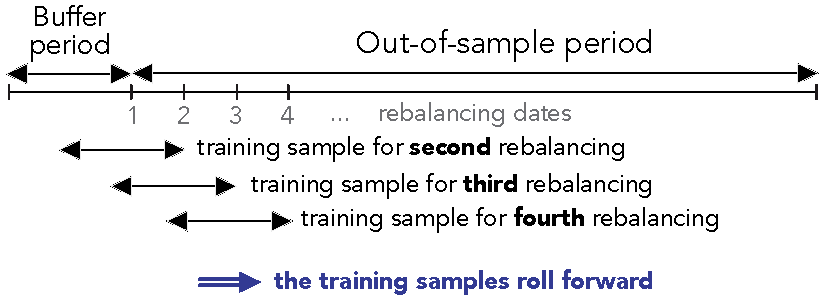
\includegraphics[width=0.7\linewidth]{files/backtestoos-a227bd2c5d9c2de16fff5346ebfdc064.pdf}
\caption[]{Backtesting with rolling windows. The training set of the first period is simply the buffer period.}
\label{fig-backtestoos}
\end{figure}

Two crucial design choices are the \textbf{rebalancing frequency} and the \textbf{horizon} at which the label is computed. It is not obvious that they should be equal but their choice should make sense. It can seem right to train on a 12-month forward label (which captures longer trends) and invest monthly or quarterly. However, it seems odd to do the opposite and train on short-term movements (monthly) and invest at a long horizon.

These choices have a direct impact on how the backtest is carried out. If we note:

\begin{itemize}
\item $\Delta_h$ for the holding period between 2 rebalancing dates (in days or months);
\item $\Delta_s$ for the size of the desired training sample (in days or months - not taking the number of assets into consideration);
\item $\Delta_l$ for the horizon at which the label is computed (in days or months),
\end{itemize}

then the total length of the training sample should be $\Delta_s+\Delta_l$. Indeed, at any moment $t$, the training sample should stop at $t -\Delta_l$ so that the last point corresponds to a label that is calculated until time $t$. This is highlighted in the figure below in the form of the red danger zone. We call it the red zone because any observation which has a time index $s$ inside the interval $(t -\Delta_l,t]$ will engender a forward looking bias. Indeed if a feature is indexed by $s \in (t -\Delta_l,t]$, then by definition, the label covers the period $[s,s+\Delta_l]$ with $s+\Delta_l>t$. At time $t$, this requires knowledge of the future and is naturally not realistic.

\begin{figure}[!htbp]
\centering
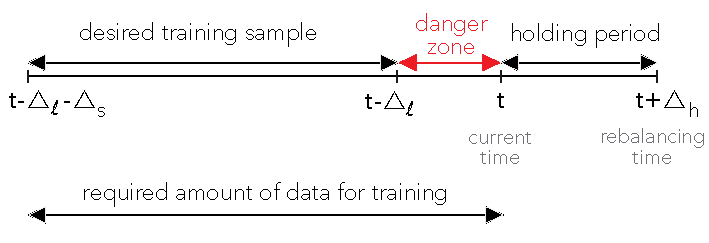
\includegraphics[width=0.7\linewidth]{files/backtestoos2-47b34e3efaf3fcd5fe3de35d9717b0da.pdf}
\caption[]{The subtleties in rolling training samples.}
\label{fig-backtestoos2}
\end{figure}

\subsubsection{Turning signals into portfolio weights}

The predictive tools outlined in Chapters \href{/chap-06-lasso}{Penalized regressions and sparse hedging for minimum variance portfolios} to \href{/chap-14-ensemble}{Ensemble models} are only meant to provide a signal that is expected to give some information on the future profitability of assets. There are many ways that this signal can be integrated in an investment decision (see \cite{snow2020machine} for ways to integrate ML tools into this task). \cite{guidolin2025machine} provide a broader recent survey, covering systematic trading, weight optimization, smart beta, textual analysis and trade execution.

First and foremost, there are at least two steps in the portfolio construction process and the signal can be used at any of these stages. Relying on the signal for both steps puts a lot of emphasis on the predictions and should only be considered when the level of confidence in the forecasts is high.

The first step is \textbf{selection}. While a forecasting exercise can be carried out on a large number of assets, it is not compulsory to invest in all of these assets. In fact, for long-only portfolios, it would make sense to take advantage of the signal to exclude those assets that are presumably likely to underperform in the future. Often, portfolio policies have fixed sizes that impose a constant number of assets. One heuristic way to exploit the signal is to select the assets that have the most favorable predictions and to discard the others. This naive idea is often used in the asset pricing literature: portfolios are formed according to the quantiles of underlying characteristics and some characteristics are deemed interesting if the corresponding \textbf{sorted portfolios} exhibit very different profitabilities (e.g., high average return for high quantiles versus low average return for low quantiles).

This is for instance an efficient way to test the relevance of the signal. If $Q$ portfolios $q=1,\dots,Q$ are formed according to the rankings of the assets with respect to the signal, then one would expect that the out-of-sample performance of the portfolios be monotonic with $q$. While a rigorous test of monotonicity would require to account for all portfolios (see, e.g., \cite{romano2013testing}), it is often only assumed that the extreme portfolios suffice. If the difference between portfolio number 1 and portfolio number $Q$ is substantial, then the signal is valuable. Whenever the investor is able to short assets, this amounts to a dollar neutral strategy.

Selection based on simple quantile sorts can be improved. \cite{poh2020building} cast stock selection as a ranking problem and show that learning to rank algorithms, trained on pairwise or listwise comparisons rather than on a pointwise loss, roughly triple the Sharpe ratio of a cross sectional momentum strategy compared to standard regression based sorts. \cite{feng2019deep} push the sorting step itself into a deep network: firm characteristics are mapped into long short portfolio weights through a nonlinear activation trained to minimize pricing errors rather than forecast error, generalizing the usual characteristic sort. Combining several signals also matters. \cite{muller2021interacting} study every possible double sorted portfolio built from 102 anomalies and find that hundreds of interactions remain significant after correcting for the resulting multiple testing problem. \cite{guidetti2025trust} instead borrow a Majority Judgment ranking method from social choice theory to aggregate several anomalies into one portfolio, and show that this aggregation is more robust to the choice of rebalancing schedule and weighting scheme than simple z score or rank averaging.

The second step is \textbf{weighting}. If the selection process relied on the signal, then a simple weighting scheme is often a good idea. Equally weighted portfolios are known to be hard to beat (see \cite{demiguel2007optimal}), especially compared to their cap-weighted alternative, as is shown in \cite{plyakha2014equal}. More advanced schemes include equal risk contributions \citep{maillard2010properties} and constrained minimum variance \citep{coqueret2015diversified}. Both only rely on the covariance matrix of the assets and not on any proxy for the vector of expected returns.

For the sake of completeness, we explicitize a generalization of \cite{coqueret2015diversified} which is a generic constrained quadratic program:

\begin{equation}
\label{eq:coq}
\underset{\textbf{w}}{\text{min}} \ \frac{\lambda}{2} \textbf{w}'\boldsymbol{\Sigma}\textbf{w}-\textbf{w}'\boldsymbol{\mu} , \quad \text{s.t.} \quad \begin{array}{ll} \textbf{w}'\textbf{1}=1, \\ (\textbf{w}-\textbf{w}_-)'\boldsymbol{\Lambda}(\textbf{w}-\textbf{w}_-) \le \delta_R,\\
\textbf{w}'\textbf{w} \le \delta_D,
\end{array}
\end{equation}

where it is easy to recognize the usual \textbf{mean-variance optimization} in the left-hand side. We impose three constraints on the right-hand side. The first one is the budget constraint (weights sum to one). The second one penalizes variations in weights (compared to the current allocation, $\textbf{w}_ -$) via a diagonal matrix $\boldsymbol{\Lambda}$ that penalizes trading costs. This is a crucial point. Portfolios are rarely constructed from scratch and are most of the time \textbf{adjustments} from existing positions. In order to reduce the orders and the corresponding transaction costs, it is possible to penalize large variations from the existing portfolio. In the above program, the current weights are written $\textbf{w}_ -$ and the desired ones $\textbf{w}$ so that $\textbf{w} -\textbf{w}_ -$ is the vector of deviations from the current positions. The term $(\textbf{w} -\textbf{w}_ -)'\boldsymbol{\Lambda}(\textbf{w} -\textbf{w}_ -)$ is an expression that characterizes the sum of squared deviations, weighted by the diagonal coefficients $\Lambda_{n,n}$. This can be helpful because some assets may be more costly to trade due to liquidity (large cap stocks are more liquid and their trading costs are lower). When $\delta_R$ decreases, the rotation is reduced because weights are not allowed too deviate too much from $\textbf{w}_ -$. The last constraint enforces \textbf{diversification} via the Herfindhal-Hirschmann index of the portfolio: the smaller $\delta_D$, the more diversified the portfolio.

Recalling that there are $N$ assets in the universe, the Lagrange form of \ref{eq:coq} is:

\begin{equation}
\label{eq:lagrangew}
L(\textbf{w})= \frac{\lambda}{2} \textbf{w}'\boldsymbol{\Sigma}\textbf{w}-\textbf{w}'\boldsymbol{\mu}-\eta (\textbf{w}'\textbf{1}_N-1)+\kappa_R ( (\textbf{w}-\textbf{w}_-)'\boldsymbol{\Lambda}(\textbf{w}-\textbf{w}_-) - \delta_R)+\kappa_D(\textbf{w}'\textbf{w}-\delta_D),
\end{equation}

and the first order condition

\begin{equation}
\frac{\partial}{\partial \textbf{w}}L(\textbf{w})= \lambda \boldsymbol{\Sigma}\textbf{w}-\boldsymbol{\mu}-\eta\textbf{1}_N+2\kappa_R \boldsymbol{\Lambda}(\textbf{w}-\textbf{w}_-)+2\kappa_D\textbf{w}=0,
\end{equation}

yields

\begin{equation}
\label{eq:coqw}
\textbf{w}^*_\kappa=  (\lambda \boldsymbol{\Sigma}+2\kappa_R \boldsymbol{\Lambda} +2\kappa_D\textbf{I}_N)^{-1} \left(\boldsymbol{\mu} + \eta_{\lambda,\kappa_R,\kappa_D} \textbf{1}_N+2\kappa_R \boldsymbol{\Lambda}\textbf{w}_-\right),
\end{equation}

with

\begin{equation}
\eta_{\lambda,\kappa_R,\kappa_D}=\frac{1- \textbf{1}_N'(\lambda\boldsymbol{\Sigma}+2\kappa_R \boldsymbol{\Lambda}+2\kappa_D\textbf{I}_N)^{-1}(\boldsymbol{\mu}+2\kappa_R\boldsymbol{\Lambda}\textbf{w}_-)}{\textbf{1}'_N(\lambda \boldsymbol{\Sigma}+2\kappa_R \boldsymbol{\Lambda}+2\kappa_D\textbf{I}_N)^{-1}\textbf{1}_N}.
\end{equation}

This parameter ensures that the budget constraint is satisfied. The optimal weights in \ref{eq:coqw} depend on three tuning parameters: $\lambda$, $\kappa_R$ and $\kappa_D$.

\begin{itemize}
\item When $\lambda$ is large, the focus is set more on risk reduction than on profit maximization (which is often a good idea given that risk is easier to predict);
\item When $\kappa_R$ is large, the importance of transaction costs in \ref{eq:lagrangew} is high and thus, in the limit when $\kappa_R \rightarrow \infty$, the optimal weights are equal to the old ones $\textbf{w}_ -$ (for finite values of the other parameters).
\item When $\kappa_D$ is large, the portfolio is more diversified and (all other things equal) when $\kappa_D \rightarrow \infty$, the weights are all equal (to $1/N$).
\item When $\kappa_R=\kappa_D=0$, we recover the classical mean-variance weights which are a mix between the maximum Sharpe ratio portfolio proportional to $(\boldsymbol{\Sigma})^{ -1} \boldsymbol{\mu}$ and the minimum variance portfolio proportional to $(\boldsymbol{\Sigma})^{ -1} \textbf{1}_N$.
\end{itemize}

This seemingly complex formula is in fact very flexible and tractable. It requires some tests and adjustments before finding realistic values for $\lambda$, $\kappa_R$ and $\kappa_D$ (see exercise at the end of the chapter). In \cite{pedersen2020enhanced}, the authors recommend a similar form, except that the covariance matrix is shrunk towards the diagonal matrix of sample variances and the expected returns are mix between a signal and an anchor portfolio. The authors argue that their general formulation has links with robust optimization (see also \cite{kim2014deciphering}), Bayesian inference \citep{lai2011mean}, matrix denoising via random matrix theory, and, naturally, \textbf{shrinkage}. In fact, shrunk expected returns have been around for quite some time (\cite{jorion1985international}, \cite{kan2007optimal} and \cite{bodnar2013equivalence}) and simply seek to diversify and reduce estimation risk.

An older and simpler alternative to the quadratic program above is the parametric portfolio policy of \cite{brandt2009parametric}, which maps characteristics directly into weights through a small parameter vector and sidesteps the need to model returns explicitly. \cite{connor2021dynamic} extend this idea into a two step semiparametric model where a first stage builds factor mimicking sub portfolios and a second stage combines them dynamically using expected utility. Recent work corrects a blind spot of the original policy: it treats the estimated parameter as if it were the truth and so ignores policy risk. \cite{herculano2026bayesian} and \cite{lamoureux2026gibbs} both place a Bayesian prior on the policy coefficients, using two different generalized Bayesian formulations, and find sizably higher Sharpe ratios, lower turnover and lower tail risk once this estimation risk is accounted for, especially during crises. \cite{simon2025deep} instead replace the linear policy with a deep network and show that risk aversion acts as a natural regularizer that keeps the added complexity in check.

A more direct route skips the return forecast altogether and learns portfolio weights straight from characteristics. \cite{bell2026alphaglass} propose an interpretable model that maps characteristics into additive signals with sparse interactions and converts them into long short weights through a differentiable rank and mask layer, optimizing the Sharpe ratio end to end while keeping the drivers of each position traceable. \cite{you2025markowitz} and \cite{wang2026machine} pursue a similar end to end philosophy from different angles: the first turns the whole mean variance program into an unconstrained learning task, while the second lets each investor's own risk preferences and constraints shape the prediction stage rather than being added afterward. \cite{coulombe2023maximally} take yet another direction and optimize weights so that the resulting portfolio return is maximally predictable in itself, combining a random forest and a constrained ridge regression to extend earlier maximally predictable portfolio approaches based on linear factors. Finally, since all of these approaches still need an estimate of expected returns, \cite{asimit2025distribution} propose a distribution free shrinkage estimator of the mean vector that improves both return prediction and mean variance portfolios in high dimension.

\subsubsection{Performance metrics}

The evaluation of performance is a key stage in a backtest. This section, while not exhaustive, is intended to cover the most important facets of portfolio assessment.

\paragraph{Discussion}

While the evaluation of the accuracy of ML tools (See \ref{sec_mlmetrics}) is of course valuable (and imperative!), the portfolio returns are the ultimate yardstick during a backtest. One essential element in such an exercise is a \textbf{benchmark} because raw and absolute metrics don't mean much on their own.

This is not only true at the portfolio level, but also at the ML engine level. In most of the trials of the previous chapters, the MSE of the models on the testing set revolves around 0.037. An interesting figure is the variance of one-month returns on this set, which corresponds to the error made by a constant prediction of 0 all the time. This benchmark is the one used in the out-of-sample $R^2$ of \cite{gu2018empirical}.

This gap between statistical accuracy and portfolio performance is not a minor detail. \cite{salcher2026lost} show that MSE based measures of forecast accuracy can be weakly or even negatively correlated with the Sharpe ratio of the resulting portfolio. They propose a risk adjusted forecast error measure built on the Mahalanobis distance, which weights forecast errors by the inverse covariance of returns and thus penalizes mistakes on exactly the low risk, high return looking positions that mean variance optimization tends to overweight. Their simulations and empirical application confirm that this measure tracks the Sharpe ratio gap far better than plain RMSE.

In portfolio choice, the most elementary allocation is the uniform one, whereby each asset receives the same weight. This seemingly simplistic solution is in fact an incredible benchmark, one that is hard to beat consistently (see \cite{demiguel2007optimal} and \cite{plyakha2014equal}). Theoretically, uniform portfolios are optimal when uncertainty, ambiguity or estimation risk is high (\cite{pflug20121}, \cite{maillet2015global}, \cite{zhao2021efficient}) and empirically, it cannot be outperformed even at the factor level \citep{dichtl2020build}. Below, we will pick an \textbf{equally weighted} (EW) portfolio of all stocks as our benchmark.

\paragraph{Pure performance and risk indicators}

We then turn to the definition of the usual metrics used both by practitioners and academics alike. Henceforth, we write $r^P=(r_t^P)_{1\le t\le T}$ and $r^B=(r_t^B)_{1\le t\le T}$ for the returns of the portfolio and those of the benchmark, respectively. When referring to some generic returns, we simply write $r_t$. There are many ways to analyze them and most of them rely on their distribution.

The simplest indicator is the average return:

\begin{equation}
\bar{r}_P=\mu_P=\mathbb{E}[r^P]\approx \frac{1}{T}\sum_{t=1}^T r_t^P, \quad \bar{r}_B=\mu_B=\mathbb{E}[r^B]\approx \frac{1}{T}\sum_{t=1}^T r_t^B,
\end{equation}

where, obviously, the portfolio is noteworthy if $\mathbb{E}[r^P]>\mathbb{E}[r^B]$. Note that we use the arithmetic average above but the geometric one is also an option, in which case:

\begin{equation}
\tilde{\mu}_P\approx \left(\prod_{t=1}^T(1+r^P_t) \right)^{1/T}-1 , \quad \tilde{\mu}_B \approx  \left(\prod_{t=1}^T(1+r^B_t) \right)^{1/T}-1.
\end{equation}

The benefit of this second definition is that it takes the compounding of returns into account and hence compensates for volatility pumping. To see this, consider a very simple two-period model with returns $-r$ and $+r$. The arithmetic average is zero, but the geometric one $\sqrt{1 -r^2} -1$ is negative.

Akin to accuracy, it ratios evaluate the proportion of times when the position is in the right direction (long when the realized return is positive and short when it is negative). Hence hit ratios evaluate the propensity to make \textit{good guesses}. This can be computed at the asset level (the proportion of positions in the correct direction) or at the portfolio level. In all cases, the computation can be performed on raw returns or on relative returns (e.g., compared to a benchmark). A meaningful hit ratio is the proportion of times that a strategy beats its benchmark. This is of course not sufficient, as many small gains can be offset by a few large losses.

Pure performance measures are almost always accompanied by \textbf{risk measures}. The second moment of returns is usually used to quantify the magnitude of fluctuations of the portfolio. A large variance implies sizable movements in returns, and hence in portfolio values. This is why the standard deviation of returns is called the \textbf{volatility} of the portfolio.

\begin{equation}
\sigma^2_P=\mathbb{V}[r^P]\approx \frac{1}{T-1}\sum_{t=1}^T (r_t^P-\mu_P)^2, \quad \sigma^2_B=\mathbb{V}[r^B]\approx \frac{1}{T-1}\sum_{t=1}^T (r_t^B-\mu_B)^2.
\end{equation}

In this case, the portfolio can be preferred if it is less risky compared to the benchmark, i.e., when $\sigma_P^2<\sigma_B^2$ and when average returns are equal (or comparable).

Higher order moments of returns are sometimes used (skewness and kurtosis), but they are far less common. We refer for instance to \cite{harvey2010portfolio} for one method that takes them into account in the portfolio construction process.

For some people, the volatility is an incomplete measure of risk. It can be argued that it should be decomposed into `good' volatility (when prices go up) versus `bad' volatility when they go down. The downward semi-variance is computed as the variance taken over the negative returns:

\begin{equation}
\sigma^2_-\approx \frac{1}{\text{card}(r_t<0)}\sum_{t=1}^T (r_t-\mu_P)^21_{\{r_t<0\}}.
\end{equation}

The average return and the volatility are the typical moment-based metrics used by practitioners. Other indicators rely on different aspects of the distribution of returns with a focus on tails and extreme events. The \textbf{Value-at-Risk} (VaR) is one such example. If $F_r$ is the empirical cdf of returns, the VaR at a level of confidence $\alpha$ (often taken to be 95\%) is

\begin{equation}
\text{VaR}_\alpha(\textbf{r}_t)=F_r(1-\alpha).
\end{equation}

It is equal to the realization of a bad scenario (of return) that is expected to happen $(1 -\alpha)$\% of the time on average.
An even more conservative measure is the so-called \textbf{Conditional Value at Risk} (CVaR), also known as expected shortfall, which computes the average loss of the worst ($1 -\alpha$)\% scenarios. Its empirical evaluation is

\begin{equation}
\text{CVaR}_\alpha(\textbf{r}_t)=\frac{1}{\text{Card}(r_t < \text{VaR}_\alpha(\text{r}_t))}\sum_{r_t < \text{VaR}_\alpha(\text{r}_t)}r_t.
\end{equation}

Going crescendo in the severity of risk measures, the ultimate evaluation of loss is the \textbf{maximum drawdown}. It is equal to the maximum loss suffered from the peak value of the strategy. If we write $P_t$ for the time-$t$ value of a portfolio, the drawdown is

\begin{equation}
D_T^P=\underset{0 \le t \le T}{\text{max}} P_t-P_T ,
\end{equation}

and the maximum drawdown is

\begin{equation}
MD_T^P=\underset{0 \le s \le T}{\text{max}} \left(\underset{0 \le t \le s}{\text{max}} P_t-P_s, 0\right) .
\end{equation}

This quantity evaluates the greatest loss over the time frame $[0,T]$ and is thus the most conservative risk measure of all.

\paragraph{Factor-based evaluation}

In the spirit of factor models, performance can also be assessed through the lens of exposures. If we recall the original formulation from Equation \ref{eq:apt}:

\begin{equation}
r_{t,n}= \alpha_n+\sum_{k=1}^K\beta_{t,k,n}f_{t,k}+\epsilon_{t,n},
\end{equation}

then the estimated $\hat{\alpha}_n$ is the performance that cannot be explained by the other factors. When returns are \textit{excess} returns (over the risk-free rate) and when there is only one factor, the market factor, then this quantity is called Jensen's alpha \citep{jensen1968performance}. Often, it is simply referred to as \textit{alpha}. The other estimate, $\hat{\beta}_{t,M,n}$ ($M$ for market), is the market beta.

Because of the rise of factor investing, it has become customary to also report the alpha of more exhaustive regressions. Adding the size and value premium (as in \cite{fama1993common}) and even momentum \citep{carhart1997persistence} helps understand if a strategy generates value beyond that which can be obtained through the usual factors.

\paragraph{Risk-adjusted measures}

Now, the tradeoff between the average return and the volatility is a cornerstone in modern finance, since \cite{markowitz1952portfolio}. The simplest way to synthesize both metrics is via the \textbf{information ratio}:

\begin{equation}
IR(P,B)=\frac{\mu_{P-B}}{\sigma_{P-B}},
\end{equation}

where the index $P -B$ implies that the mean and standard deviations are computed on the long-short portfolio with returns $r_t^P -r_t^B$. The denominator $\sigma_{P -B}$ is sometimes called the \textbf{tracking error}.

The most widespread information ratio is the \textbf{Sharpe ratio} \citep{sharpe1966mutual} for which the benchmark is some riskless asset. Instead of directly computing the information ratio between two portfolios or strategies, it is often customary to compare their Sharpe ratios. Simple comparisons can benefit from statistical tests (see, e.g., \cite{ledoit2008robust}).

More extreme risk measures can serve as denominator in risk-adjusted indicators. The Managed Account Report (MAR) ratio is, for example, computed as

\begin{equation}
MAR^P = \frac{\tilde{\mu}_P}{MD^P},
\end{equation}

while the Treynor ratio is equal to

\begin{equation}
\text{Treynor}=\frac{\mu_P}{\hat{\beta}_M},
\end{equation}

i.e., the (excess) return divided by the market beta (see \cite{treynor1965rate}). This definition was generalized to multifactor expositions by \cite{hubner2005generalized} into the generalized Treynor ratio:

\begin{equation}
\text{GT}=\mu_P\frac{\sum_{k=1}^K\bar{f}_k}{\sum_{k=1}^K\hat{\beta}_k\bar{f}_k},
\end{equation}

where the $\bar{f}_k$ are the sample average of the factors $f_{t,k}$. We refer to the original article for a detailed account of the analytical properties of this ratio.

\paragraph{Transaction costs and turnover}

Updating portfolio composition is not free. In all generality, the total cost of one rebalancing at time $t$ is proportional to $C_t=\sum_{n=1}^N | \Delta w_{t,n}|c_{t,n}$, where $\Delta w_{t,n}$ is the change in position for asset $n$ and $c_{t,n}$ the corresponding fee. This last quantity is often hard to predict, thus it is customary to use a proxy that depends for instance on market capitalization (large stocks have more liquid shares and thus require smaller fees) or bid-ask spreads (smaller spreads mean smaller fees).

As a first order approximation, it is often useful to compute the average turnover:

\begin{equation}
\text{Turnover}=\frac{1}{T-1}\sum_{t=2}^T\sum_{n=1}^N|w_{t,n}-w_{t-,n}|,
\end{equation}

where $w_{t,n}$ are the desired $t$-time weights in the portfolio and $w_{t -,n}$ are the weights just before the rebalancing. The positions of the first period (launching weights) are exluded from the computation by convention. Transaction costs can then be proxied as a multiple of turnover (times some average or median cost in the cross-section of firms). This is a first order estimate of realized costs that does not take into consideration the evolution of the scale of the portfolio. Nonetheless, a rough figure is much better than none at all.

Once transaction costs (TCs) have been annualized, they can be deducted from average returns to yield a more realistic picture of profitability. In the same vein, the transaction cost-adjusted Sharpe ratio of a portfolio $P$ is given by

\begin{equation}
\label{eq:SRTC}
SR_{TC}=\frac{\mu_P-TC}{\sigma_P}.
\end{equation}

Transaction costs are often overlooked in academic articles but can have a sizable impact in real life trading (see, e.g., \cite{novy2015taxonomy}). \cite{martin2018transaction} show how to use factor investing (and exposures) to combine and offset positions and reduce overall fees.

Two recent papers add further caution here. \cite{yin2026implementation} run fifteen benchmark strategies through five independent backtesting engines and show that, once nonzero transaction costs enter the picture, the choice of engine alone can move total returns by several percentage points for high turnover strategies, driven largely by undocumented differences in how each engine applies cost models. \cite{beckmeyer2026reviving} turn this around into a constructive framework: by combining machine learning return forecasts with scale dependent transaction cost estimates, they identify which anomalies remain profitable net of costs for funds of a given size, and show that a simple equally weighted basket of these implementable anomalies still delivers Sharpe ratios between 0.64 and 1.01.

\subsubsection{Common errors and issues}

\paragraph{Forward looking data}

One of the most common mistakes in portfolio backtesting is the use of forward looking data. It is for instance easy to fall in the trap of the danger zone depicted in Figure~\ref{fig-backtestoos2}. In this case, the labels used at time $t$ are computed with knowledge of what happens at times $t+1$, $t+2$, etc. It is worth triple checking every step in the code to make sure that strategies are not built on prescient data.

\paragraph{Backtest overfitting}\label{backov}

The second major problem is backtest overfitting. The analogy with training set overfitting is easy to grasp. It is a well-known issue and was formalized for instance in \cite{white2000reality} and \cite{romano2005stepwise}. In portfolio choice, we refer to \cite{bajgrowicz2012technical}, \cite{bailey2014deflated} and \cite{lopez2020false}, and the references therein.

At any given moment, a backtest depends on \textit{only} one particular dataset. Often, the result of the first backtest will not be satisfactory - for many possible reasons. Hence, it is tempting to have another try, when altering some parameters that were probably not optimal. This second test may be better, but not quite good enough - yet. Thus, in a third trial, a new weighting scheme can be tested, along with a new forecasting engine (more sophisticated). Iteratively, the backtester can only end up with a strategy that performs well enough, it is just a matter of time and trials.

One consequence of backtest overfitting is that it is illusory to hope for the same Sharpe ratios in live trading as those obtained in the backtest. Reasonable professionals divide the Sharpe ratio by two at least (\cite{harvey2015backtesting}, \cite{suhonen2017quantifying}). In \cite{bailey2014deflated}, the authors even propose a statistical test for Sharpe ratios, provided that some metrics of all tested strategies are stored in memory. The formula for deflated Sharpe ratios is:

\begin{equation}
\label{eq:tSR}
t = \phi\left((SR-SR^*)\sqrt{\frac{T-1}{1-\gamma_3SR+\frac{\gamma_4-1}{4}SR^2}} \right),
\end{equation}

where $SR$ is the Sharpe Ratio obtained by the best strategy among all that were tested, and

\begin{equation}
SR^*=\mathbb{E}[SR]+\sqrt{\mathbb{V}[SR]}\left((1-\gamma)\phi^{-1}\left(1-\frac{1}{N}\right)+\gamma \phi^{-1}\left(1-\frac{1}{Ne}\right)  \right),
\end{equation}

is the theoretical average maximum SR. Moreover,

\begin{itemize}
\item $T$ is the number of trading dates;
\item $\gamma_3$ and $\gamma_4$ are the $skewness$ and $kurtosis$ of the returns of the chosen (best) strategy;
\item $\phi$ is the cdf of the standard Gaussian law and $\gamma\approx 0,577$ is the Euler-Mascheroni constant;
\item $N$ refers to the number of strategy trials.
\end{itemize}

If $t$ defined above is below a certain threshold (e.g., 0.95), then the $SR$ cannot be deemed significant: \textbf{the best strategy is not outstanding} compared to all of those that were tested. Most of the time, sadly, that is the case. In Equation \ref{eq:tSR}, the realized SR must be above the theoretical maximum $SR^*$ and the scaling factor must be sufficiently large to push the argument inside $\phi$ close enough to two, so that $t$ surpasses 0.95.

Two recent papers quantify backtest fragility from angles that complement the deflated Sharpe ratio above. \cite{chen2025design} fit more than a thousand machine learning models that only differ in seemingly minor design choices, such as the target variable, the training window or how predictions are post processed, and find that the resulting spread in portfolio returns, what they call the nonstandard error, exceeds the usual standard error by 59\%. \cite{paskaramoorthy2025bias} tackle a different source of fragility: resampling returns as if they were independent and identically distributed, a common fix for short backtests, disrupts the autocorrelation structure of returns and biases the Sharpe ratio of rolling window mean variance portfolios. They show the bias is often a modest fraction of ordinary estimation noise, but derive simple bounds, based on first lag autocorrelation, to help flag when it is not.

In the scientific community, test overfitting is also known as \textit{p}-hacking. It is rather common in financial economics and the reading of \cite{harvey2017presidential} is strongly advised to grasp the magnitude of the phenomenon. \textit{p}-hacking is also present in most fields that use statistical tests (see, e.g., \cite{head2015extent} to cite but one reference). There are several ways to cope with \textit{p}-hacking:

\begin{enumerate}
\item don't rely on \textit{p}-values \citep{amrhein2019scientists};
\item use detection tools \citep{elliott2019detecting};
\item or, finally, use advanced methods that process arrays of statistics (e.g., the Bayesianized versions of \textit{p}-values to include some prior assessment from \cite{harvey2017presidential}, or other tests such as those proposed in \cite{romano2005stepwise} and \cite{simonsohn2014p}).
\end{enumerate}

The first option is wise, but the drawback is that the decision process is then left to another arbitrary yardstick.

\paragraph{Simple safeguards}

As is mentioned at the beginning of the chapter, two common sense references for backtesting are \cite{fabozzi2018being} and \cite{arnott2019backtesting}. The pieces of advice provided in these two articles are often judicious and thoughtful.

One additional comment pertains to the output of the backtest. One simple, intuitive and widespread metric is the transaction cost-adjusted Sharpe ratio defined in Equation \ref{eq:SRTC}. In the backtest, let us call $SR_{TC}^B$ the corresponding value for the benchmark, which we like to define as the equally-weighted portfolio of all assets in the trading universe (in our dataset, roughly one thousand US equities). If the $SR_{TC}^P$ of the best strategy is above $2\times SR_{TC}^B$, then there is probably a glitch somewhere in the backtest.

This criterion holds under two assumptions:

\begin{enumerate}
\item a sufficiently long enough out-of-sample period and
\item long-only portfolios.
\end{enumerate}

It is unlikely that any realistic strategy can outperform a solid benchmark by a very wide margin over the long term. Being able to improve the benchmark's annualized return by 150 basis points (with comparable volatility) is already a great achievement. Backtests that deliver returns more than 5\% above those of the benchmark are dubious.

\subsubsection{Implication of non-stationarity: forecasting is hard}

This subsection is split into two parts: in the first, we discuss the reason that makes forecasting such a difficult task and in the second we present an important theoretical result originally developed towards machine learning but that sheds light on any discipline confronted with out-of-sample tests. An interesting contribution related to this topic is the study from \cite{farmer2019pockets}. The authors assess the predictive fit of linear models through time: they show that the fit is strongly varying: sometimes the model performs very well, sometimes, not so much. There is no reason why this should not be the case for ML algorithms as well.

\paragraph{General comments}

The careful reader must have noticed that throughout Chapters \href{/chap-06-lasso}{Penalized regressions and sparse hedging for minimum variance portfolios} to \href{/chap-14-ensemble}{Ensemble models}, the performance of ML engines is underwhelming. These disappointing results are there on purpose and highlight the crucial truth that machine learning is no panacea, no magic wand, no philosopher's stone that can transform data into golden predictions. Most ML-based forecasts fail. This is in fact not only true for very enhanced and sophisticated techniques, but also for simpler econometric approaches \citep{dichtl2019data}, which again underlines the need to replicate results to challenge their validity.

One reason for that is that datasets are full of noise and extracting the slightest amount of signal is a tough challenge (we recommend a careful reading of the introduction of \cite{timmermann2018forecasting} for more details on this topic). One rationale for that is the ever time-varying nature of factor analysis in the equity space. Some factors can perform very well during one year and then poorly the next year and these reversals can be costly in the context of fully automated data-based allocation processes.

In fact, this is one major difference with many fields for which ML has made huge advances. In image recognition, numbers will always have the same shape, and so will cats, buses, etc. Likewise, a verb will always be a verb and syntaxes in languages do not change. This invariance, though sometimes hard to grasp, is nonetheless key to the great improvement both in computer vision and natural language processing.

In factor investing, there does not seem to be such invariance (see \cite{cornell2020stock}). There is no factor and no (possibly nonlinear) combination of factors that can explain and accurately forecast returns over long periods of several decades. The academic literature has yet to find such a model; but even if it did, a simple arbitrage reasoning would logically invalidate its conclusions in future datasets.

Two recent papers reinforce this message with direct evidence. \cite{esakia2025what} decompose the gains from machine learning factor models into a richer information set and a more flexible functional form, and show that once microcaps are excluded, transaction costs are imposed and short selling is restricted, the benefit of nonlinearity nearly disappears while the benefit of richer information persists only partially. \cite{lu2025machine} push further and show that a simple economically motivated arbitrage strategy can replicate most of the apparent alpha of neural network based long short portfolios, once unpublished anomalies and microcap stocks are excluded. What looks like a black box uncovering hidden patterns is often, on closer inspection, an old and well understood economic mechanism wearing a new coat.

\paragraph{The no free lunch theorem}

We start by underlying that the no free lunch theorem in machine learning has nothing to do with the asset pricing condition with the same name (see, e.g., \cite{delbaen1994general}, or, more recently, \cite{cuchiero2016new}). The original formulation was given by \cite{wolpert1992connection} but we also recommend a look at the more recent reference \cite{ho2002simple}. There are in fact several theorems and two of them can be found in \cite{wolpert1997no}.

The statement of the theorem is very abstract and requires some notational conventions. We assume that any training sample $S=(\{\textbf{x}_1,y_1\}, \dots, \{\textbf{x}_I,y_I\})$ is such that there exists an oracle function $f$ that perfectly maps the features to the labels: $y_i=f(\textbf{x}_i)$. The oracle function $f$ belongs to a very large set of functions $\mathcal{F}$. In addition, we write $\mathcal{H}$ for the set of functions to which the forecaster will resort to approximate $f$. For instance, $\mathcal{H}$ can be the space of feed-forward neural networks, or the space of decision trees, or the reunion of both. Elements of $\mathcal{H}$ are written $h$ and $\mathbb{P}[h|S]$ stands for the (largely unknown) distribution of $h$ knowing the sample $S$. Similarly, $\mathbb{P}[f|S]$ is the distribution of oracle functions knowing $S$. Finally, the features have a given law, $\mathbb{P}[\textbf{x}]$.

Let us now consider two models, say $h_1$ and $h_2$. The statement of the theorem is usually formulated with respect to a classification task. Knowing $S$, the error when choosing $h_k$ induced by samples outside of the training sample $S$ can be quantified as:

\begin{equation}
\label{eq:nolunch}
E_k(S)= \int_{f,h}\int_{\textbf{x}\notin S} \underbrace{ (1-\delta(f(\textbf{x}),h_k(\textbf{x})))}_{\text{error term}} \underbrace{\mathbb{P}[f|S]\mathbb{P}[h|S]\mathbb{P}[\textbf{x}]}_{\text{distributional terms}},
\end{equation}

where $\delta(\cdot,\cdot)$ is the delta Kronecker function:

\begin{equation}
\label{eq:deltak}
\delta(x,y)=\left\{\begin{array}{ll} 0 & \text{if } x\neq y \\ 1 & \text{if } x = y \end{array} .\right.
\end{equation}

One of the no free lunch theorems states that $E_1(S)=E_2(S)$, that is, that with the sole knowledge of $S$, there can be no superior algorithm, \textit{on average}. In order to build a performing algorithm, the analyst or econometrician must have prior views on the structure of the relationship between $y$ and $\textbf{x}$ and integrate these views in the construction of the model. Unfortunately, this can also yield underperforming models if the views are incorrect.

\subsubsection{First example: a complete backtest}

We finally propose a full detailed example of one implementation of a ML-based strategy run on a careful backtest.
What follows is a generalization of the content of Section~\ref{sparseex}. In the same spirit, we split the backtest in four parts:

\begin{enumerate}
\item the creation/initialization of variables;
\item the definition of the strategies in one main function;
\item the backtesting loop itself;
\item the performance indicators.
\end{enumerate}

Accordingly, we start with initializations.

\begin{verbatim}
import pandas as pd
import numpy as np
import xgboost as xgb
import matplotlib.pyplot as plt
from datetime import timedelta
import warnings
warnings.filterwarnings('ignore')
plt.style.use('seaborn-v0_8-whitegrid')

# Building the data & import functions
from data_build import generate_data
data_ml, features, features_short, returns, stock_ids, stock_ids_short = generate_data()
\end{verbatim}

We start the backtest in 2007 in order to experience the market downturn of the Great Financial Crisis.

\begin{verbatim}
sep_oos = pd.Timestamp("2007-01-01")                         # Starting point for backtest
ticks = data_ml['fsym_id'].astype('category').cat.categories.tolist()  # List of all asset ids
N = len(ticks)                                               # Max number of assets
t_oos = data_ml.loc[data_ml['date'] > sep_oos, 'date'].unique()  # Out-of-sample dates
t_oos = pd.to_datetime(t_oos)                                # Transform to datetime
t_oos = sorted(t_oos)                                        # Sort dates
Tt = len(t_oos)                                              # Nb of dates
nb_port = 2                                                  # Nb of portfolios/strategies
portf_weights = np.zeros((Tt, nb_port, N))                   # Initialize portfolio weights
portf_returns = np.zeros((Tt, nb_port))                      # Initialize portfolio returns
\end{verbatim}

This first step is crucial, it lays the groundwork for the core of the backtest. We consider only two strategies: one ML-based and the EW (1/N) benchmark. The main (weighting) function will consist of these two components, but we define the sophisticated one in a dedicated wrapper. The ML-based weights are derived from XGBoost predictions with 80 trees, a learning rate of 0.3 and a maximum tree depth of 4. This makes the model complex but not exceedingly so. Once the predictions are obtained, the weighting scheme is simple: it is an EW portfolio over the best half of the stocks (those with above median prediction).

In the function below, all parameters (e.g., the learning rate, \textit{eta} or the number of trees \textit{nrounds}) are hard-coded. They can easily be passed in arguments next to the data inputs. One very important detail is that in contrast to the rest of the book, the label is the 12-month future return. The main reason for this is rooted in the discussion from Section~\ref{pers}. Also, to speed up the computations, we remove the bulk of the distribution of the labels and keep only the top 20\% and bottom 20\%, as is advised in \cite{coqueret2019training}. The filtering levels could also be passed as arguments.

\begin{verbatim}
def weights_xgb(train_data, test_data, features):
    """XGBoost-based weighting function."""
    train_features = train_data[features].values                    # Independent variables
    train_label = train_data['R12M'] / np.exp(train_data['vol_252']) # Dependent variable
    
    # Filter: keep only top/bottom 20%
    q20 = np.quantile(train_label, 0.2)
    q80 = np.quantile(train_label, 0.8)
    ind = (train_label < q20) | (train_label > q80)
    train_features = train_features[ind]                            # Filtered features
    train_label = train_label[ind].values                           # Filtered label
    
    train_matrix = xgb.DMatrix(data=train_features, label=train_label)  # XGB format
    
    params = {
        'eta': 0.3,                      # Learning rate
        'objective': 'reg:squarederror', # Regression objective
        'max_depth': 4,                  # Maximum depth of trees
        'verbosity': 0                   # No comments
    }
    
    fit = xgb.train(
        params=params,
        dtrain=train_matrix,
        num_boost_round=80               # Number of trees used
    )
    
    # Test sample => XGB format
    xgb_test = xgb.DMatrix(test_data[features].values)
    
    pred = fit.predict(xgb_test)                           # Single prediction
    w = (pred > np.median(pred)).astype(float)             # Keep only the 50% best predictions
    weights = w / w.sum() if w.sum() > 0 else w            # Normalize weights
    names = test_data['fsym_id'].unique()
    
    return {'weights': weights, 'names': names}            # Best predictions, equally-weighted
\end{verbatim}

Compared to the structure proposed in Section~\ref{sec_boostext}, the differences are that the label is not only based on \textbf{long-term} returns, but it also relies on a volatility component. Even though the denominator in the label is the exponential quantile of the volatility, it seems fair to say that it is inspired by the Sharpe ratio and that the model seeks to explain and forecast a risk-adjusted return instead of a \textit{raw} return. A stock with very low volatility will have its return unchanged in the label, while a stock with very high volatility will see its return divided by a factor close to three (exp(1)=2.718).

This function is then embedded in the global weighting function which only wraps two schemes: the EW benchmark and the ML-based policy.

\begin{verbatim}
def portf_compo(train_data, test_data, features, j):
    """Portfolio composition function."""
    if j == 0:                                              # This is the benchmark
        N_test = test_data['fsym_id'].nunique()             # Test data dictates allocation
        w = 1 / N_test                                      # EW portfolio
        weights = np.full(N_test, w)
        names = test_data['fsym_id'].unique()
        return {'weights': weights, 'names': names}
    
    if j == 1:                                              # This is the ML strategy
        return weights_xgb(train_data, test_data, features)
\end{verbatim}

Equipped with this function, we can turn to the main backtesting loop. Given the fact that we use a large-scale model, the computation time for the loop is large (possibly a few hours on a slow machine with CPU). Resorting to functional programming can speed up the loop (see exercise at the end of the chapter). Also, a simple benchmark equally weighted portfolio can be coded with pandas functions only.

\begin{verbatim}
m_offset = 12                                               # Offset in months for buffer period
train_size = 5                                              # Size of training set in years

for t in range(len(t_oos) - 1):                             # Stop before last date: no fwd ret.!
    if t % 24 == 0:
        print(t_oos[t])                                     # Just checking the date status
    
    current_date = t_oos[t]
    buffer_start = current_date - pd.DateOffset(days=m_offset * 30 + 365 * train_size)
    buffer_end = current_date - pd.DateOffset(days=m_offset * 30)
    
    # Rolling window with buffer
    train_data = data_ml[
        (data_ml['date'] < buffer_end) & 
        (data_ml['date'] > buffer_start)
    ]
    test_data = data_ml[data_ml['date'] == current_date]    # Test sample
    
    realized_returns = test_data['R1M'].values              # 1M holding period!
    
    for j in range(nb_port):
        temp_weights = portf_compo(train_data, test_data, features, j)  # Weights
        # Match indices: test_data stock ids vs all ticks
        ind = [ticks.index(name) for name in temp_weights['names'] if name in ticks]
        portf_weights[t, j, ind] = temp_weights['weights']  # Allocate weights
        portf_returns[t, j] = np.sum(temp_weights['weights'] * realized_returns)  # Compute returns
\end{verbatim}

\begin{verbatim}
2007-01-31 00:00:00
\end{verbatim}

\begin{verbatim}
2009-01-31 00:00:00
\end{verbatim}

\begin{verbatim}
2011-01-31 00:00:00
\end{verbatim}

\begin{verbatim}
2013-01-31 00:00:00
\end{verbatim}

\begin{verbatim}
2015-01-31 00:00:00
\end{verbatim}

\begin{verbatim}
2017-01-31 00:00:00
\end{verbatim}

\begin{verbatim}
2019-01-31 00:00:00
\end{verbatim}

\begin{verbatim}
2021-01-31 00:00:00
\end{verbatim}

\begin{verbatim}
2023-01-31 00:00:00
\end{verbatim}

\begin{verbatim}
2025-01-31 00:00:00
\end{verbatim}

There are two important comments to be made on the above code. The first comment pertains to the two parameters that are defined in the first lines. They refer to the size of the training sample (5 years) and the length of the buffer period shown in Figure~\ref{fig-backtestoos2}. This \textbf{buffer period is imperative} because the label is based on a long-term (12-month) return. This lag is compulsory to avoid any forward-looking bias in the backtest.

Below, we create a function that computes the turnover (variation in weights). It requires both the weight values as well as the returns of all assets because the weights just before a rebalancing depend on the weights assigned in the previous period, as well as on the returns of the assets that have altered these original weights during the holding period.

\begin{verbatim}
def compute_turnover(weights, asset_returns, t_oos):
    """Compute average turnover."""
    turn = np.zeros(weights.shape[1])  # One value per strategy
    
    for t in range(1, len(t_oos)):
        realized_ret = asset_returns.loc[asset_returns.index == t_oos[t]].values.flatten()
        if len(realized_ret) == 0:
            continue
        # Ensure dimensions match
        n_assets = min(len(realized_ret), weights.shape[2])
        prior_weights = weights[t-1, :, :n_assets] * (1 + realized_ret[:n_assets])
        prior_weights_norm = prior_weights / prior_weights.sum(axis=1, keepdims=True)
        prior_weights_norm = np.nan_to_num(prior_weights_norm, 0)
        turn += np.abs(weights[t, :, :n_assets] - prior_weights_norm).sum(axis=1)
    
    return turn / (len(t_oos) - 1)
\end{verbatim}

Once turnover is defined, we embed it into a function that computes several key indicators.

\begin{verbatim}
def perf_met(portf_returns, weights, asset_returns, t_oos):
    """Compute performance metrics for a single strategy."""
    avg_ret = np.nanmean(portf_returns)                     # Arithmetic mean
    vol = np.nanstd(portf_returns)                          # Volatility
    Sharpe_ratio = avg_ret / vol if vol > 0 else 0          # Sharpe ratio
    VaR_5 = np.nanquantile(portf_returns, 0.05)             # Value-at-risk
    
    # Turnover calculation
    turn = 0
    for t in range(1, len(t_oos)):
        date_mask = asset_returns.index == t_oos[t]
        if date_mask.sum() == 0:
            continue
        realized_ret = asset_returns.loc[date_mask].values.flatten()
        n_assets = min(len(realized_ret), len(weights[t-1]))
        prior_weights = weights[t-1, :n_assets] * (1 + realized_ret[:n_assets])
        prior_sum = prior_weights.sum()
        if prior_sum > 0:
            prior_weights_norm = prior_weights / prior_sum
        else:
            prior_weights_norm = prior_weights
        turn += np.abs(weights[t, :n_assets] - prior_weights_norm).sum()
    
    turn = turn / (len(t_oos) - 1)                          # Average over time
    
    return {
        'avg_ret': avg_ret,
        'vol': vol,
        'Sharpe_ratio': Sharpe_ratio,
        'VaR_5': VaR_5,
        'turn': turn
    }
\end{verbatim}

Lastly, we build a function that loops on the various strategies.

\begin{verbatim}
def perf_met_multi(portf_returns, weights, asset_returns, t_oos, strat_names):
    """Compute performance metrics for multiple strategies."""
    J = weights.shape[1]                                    # Number of strategies
    results = []
    
    for j in range(J):
        met = perf_met(portf_returns[:, j], weights[:, j, :], asset_returns, t_oos)
        results.append(met)
    
    df = pd.DataFrame(results, index=strat_names)
    return df
\end{verbatim}

Given the weights and returns of the portfolios, it remains to compute the returns of the assets to plug them in the aggregate metrics function.

\begin{verbatim}
# Compute return matrix: start from data
asset_returns = data_ml.pivot(
    index='date',
    columns='fsym_id',
    values='R1M'
)                                                           # Shape in matrix format
asset_returns = asset_returns.fillna(0)                     # Zero returns for missing points

# Compute performance metrics
met = perf_met_multi(
    portf_returns=portf_returns,
    weights=portf_weights,
    asset_returns=asset_returns,
    t_oos=t_oos,
    strat_names=["EW", "XGB_SR"]
)
met                                                         # Display perf metrics
\end{verbatim}

\bigskip\noindent
\begin{tabular}{p{\dimexpr 0.167\linewidth-2\tabcolsep}p{\dimexpr 0.167\linewidth-2\tabcolsep}p{\dimexpr 0.167\linewidth-2\tabcolsep}p{\dimexpr 0.167\linewidth-2\tabcolsep}p{\dimexpr 0.167\linewidth-2\tabcolsep}p{\dimexpr 0.167\linewidth-2\tabcolsep}}
\toprule
 & avg\_ret & vol & Sharpe\_ratio & VaR\_5 & turn \\
\hline
EW & 0.011429 & 0.057940 & 0.197258 & -0.088251 & 0.078425 \\
\hline
XGB\_SR & 0.046026 & 0.064485 & 0.713753 & -0.055471 & 0.707462 \\
\hline
\bottomrule
\end{tabular}

\bigskip

The ML-based strategy performs finally well! The gain is mostly obtained by the average return, while the volatility is higher than that of the benchmark. The net effect is that the Sharpe ratio is improved compared to the benchmark. The augmentation is not breathtaking, but (hence?) it seems reasonable. It is noteworthy to underline that turnover is substantially higher for the sophisticated strategy. Removing costs in the numerator (say, 0.005 times the turnover, as in \cite{goto2015improving}, which is a conservative figure) only mildly reduces the superiority in Sharpe ratio of the ML-based strategy.

Finally, it is always tempting to plot the corresponding portfolio values and we display two related graphs below.

\begin{figure}[!htbp]
\centering
\begin{verbatim}
fig, axes = plt.subplots(2, 1, figsize=(10, 8))

# Plot 1: Cumulative returns
cum_ret_benchmark = np.cumprod(1 + portf_returns[:, 0])
cum_ret_ml = np.cumprod(1 + portf_returns[:, 1])

axes[0].plot(t_oos, cum_ret_benchmark, label='Benchmark (EW)', linewidth=1.5)
axes[0].plot(t_oos, cum_ret_ml, label='ML-based', linewidth=1.5)
axes[0].set_xlabel('Date')
axes[0].set_ylabel('Cumulative Value')
axes[0].legend()
axes[0].set_title('Portfolio Value Over Time')

# Plot 2: Annual average returns
years = pd.to_datetime(t_oos).year
df_returns = pd.DataFrame({
    'year': years,
    'benchmark': portf_returns[:, 0],
    'ml_based': portf_returns[:, 1]
})
annual_returns = df_returns.groupby('year').mean()

x = np.arange(len(annual_returns))
width = 0.35

axes[1].bar(x - width/2, annual_returns['benchmark'], width, label='Benchmark (EW)')
axes[1].bar(x + width/2, annual_returns['ml_based'], width, label='ML-based')
axes[1].set_xlabel('Year')
axes[1].set_ylabel('Average Return')
axes[1].set_xticks(x)
axes[1].set_xticklabels(annual_returns.index, rotation=45)
axes[1].legend()
axes[1].set_title('Average Annual Returns by Strategy')

plt.tight_layout()
plt.show()
\end{verbatim}
\caption[]{Graphical representation of the performance of the portfolios.

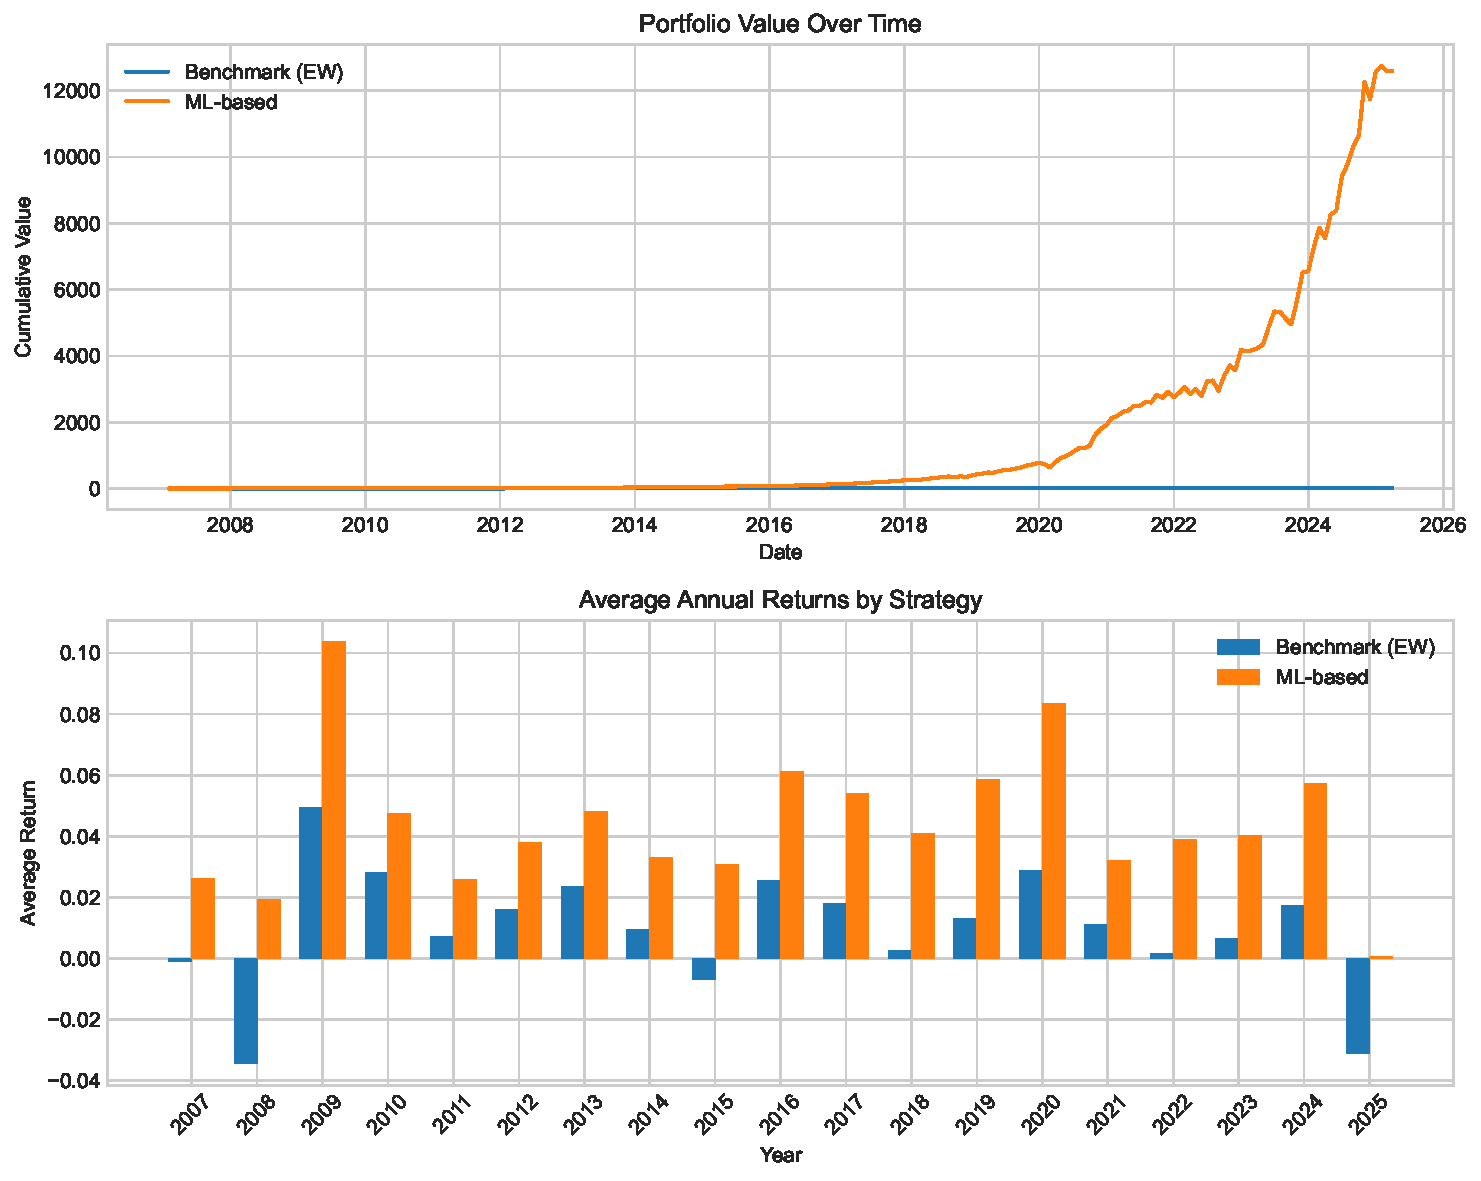
\includegraphics[width=0.7\linewidth]{files/9bfa1d0ababb282b9edbc571d38c2d42.pdf}}
\label{fig-backtest_perf}
\end{figure}

Out of the 12 years of the backtest, the advanced strategy outperforms the benchmark during 10 years. It is less hurtful in two of the four years of aggregate losses (2015 and 2018). This is a satisfactory improvement because the EW benchmark is tough to beat!

\subsubsection{Second example: backtest overfitting}

To end this chapter, we quantify the concepts of Section \ref{#backov}. First, we build a function that is able to generate performance metrics for simple strategies that can be evaluated in batches. The strategies are pure factor bets and depend on three inputs: the chosen characteristic (e.g., market capitalization), a threshold level (quantile of the characteristic) and a direction (long position in the top or bottom of the distribution).

\begin{verbatim}
def strat(data, feature, thresh, direction):
    """Compute strategy performance metrics."""
    data_tmp = data[['date', feature, 'R1M']].copy()        # Data
    
    # Investment decision
    data_tmp['decision'] = (direction * data_tmp[feature] > direction * thresh)
    
    # Date-by-date analysis
    result = data_tmp.groupby('date').apply(
        lambda x: pd.Series({
            'nb': x['decision'].sum(),
            'p_return': (x['decision'] / x['decision'].sum() * x['R1M']).sum()
                        if x['decision'].sum() > 0 else 0
        })
    ).reset_index()
    
    # Performance metrics
    avg = result['p_return'].mean()
    sd = result['p_return'].std()
    SR = avg / sd if sd > 0 else 0
    
    return {'avg': avg, 'sd': sd, 'SR': SR}
\end{verbatim}

Then, we test the function on a triplet of arguments. We pick the price-to-book (PB) ratio. The position is positive and the threshold is 0.3, which means that the strategy buys the stocks that have a PB value above the 0.3 quantile of the distribution.

\begin{verbatim}
strat(data_ml, 'PB', 0.3, 1)   # Large cap
\end{verbatim}

\begin{verbatim}
{'avg': np.float64(0.01229655670147973),
 'sd': np.float64(0.05200102503000609),
 'SR': np.float64(0.23646758298291742)}
\end{verbatim}

The output keeps three quantities that will be useful to compute the statistic \ref{eq:tSR}. We must now generate these indicators for many strategies. We start by creating the grid of parameters.

\begin{verbatim}
feature_list = ["Div_yld", "EPS", "size_avg_252d", "mom_252", "PB", "vol_252"]
thresh_list = np.arange(0.2, 0.85, 0.1)                     # Threshold values
direction_list = [1, -1]                                    # Decision direction

# Create parameter grid
from itertools import product
pars = list(product(feature_list, thresh_list, direction_list))
\end{verbatim}

This makes 84 strategies in total. We can proceed to see how they fare. We plot the corresponding Sharpe ratios below. The top plot shows the strategies that invest in the bottoms of the distributions of characteristics while the bottom plot pertains to the portfolios that are long in the lower parts of these distributions.

\begin{figure}[!htbp]
\centering
\begin{verbatim}
# Run all strategies
results = []
for feature, thresh, direction in pars:
    res = strat(data_ml, feature, thresh, direction)
    res['feature'] = feature
    res['thresh'] = thresh
    res['direction'] = direction
    results.append(res)

grd = pd.DataFrame(results)

# Plot
fig, axes = plt.subplots(2, 1, figsize=(8, 8), sharex=True)

for direction, ax in zip([1, -1], axes):
    subset = grd[grd['direction'] == direction]
    for feature in feature_list:
        data_feat = subset[subset['feature'] == feature]
        ax.plot(data_feat['thresh'], data_feat['SR'], marker='o', label=feature)
    ax.set_ylabel('Sharpe Ratio')
    ax.set_title(f'Direction = {direction}')
    ax.legend(loc='best', fontsize=8)

axes[1].set_xlabel('Threshold')
plt.tight_layout()
plt.show()
\end{verbatim}
\caption[]{Sharpe ratios of all backtested strategies.

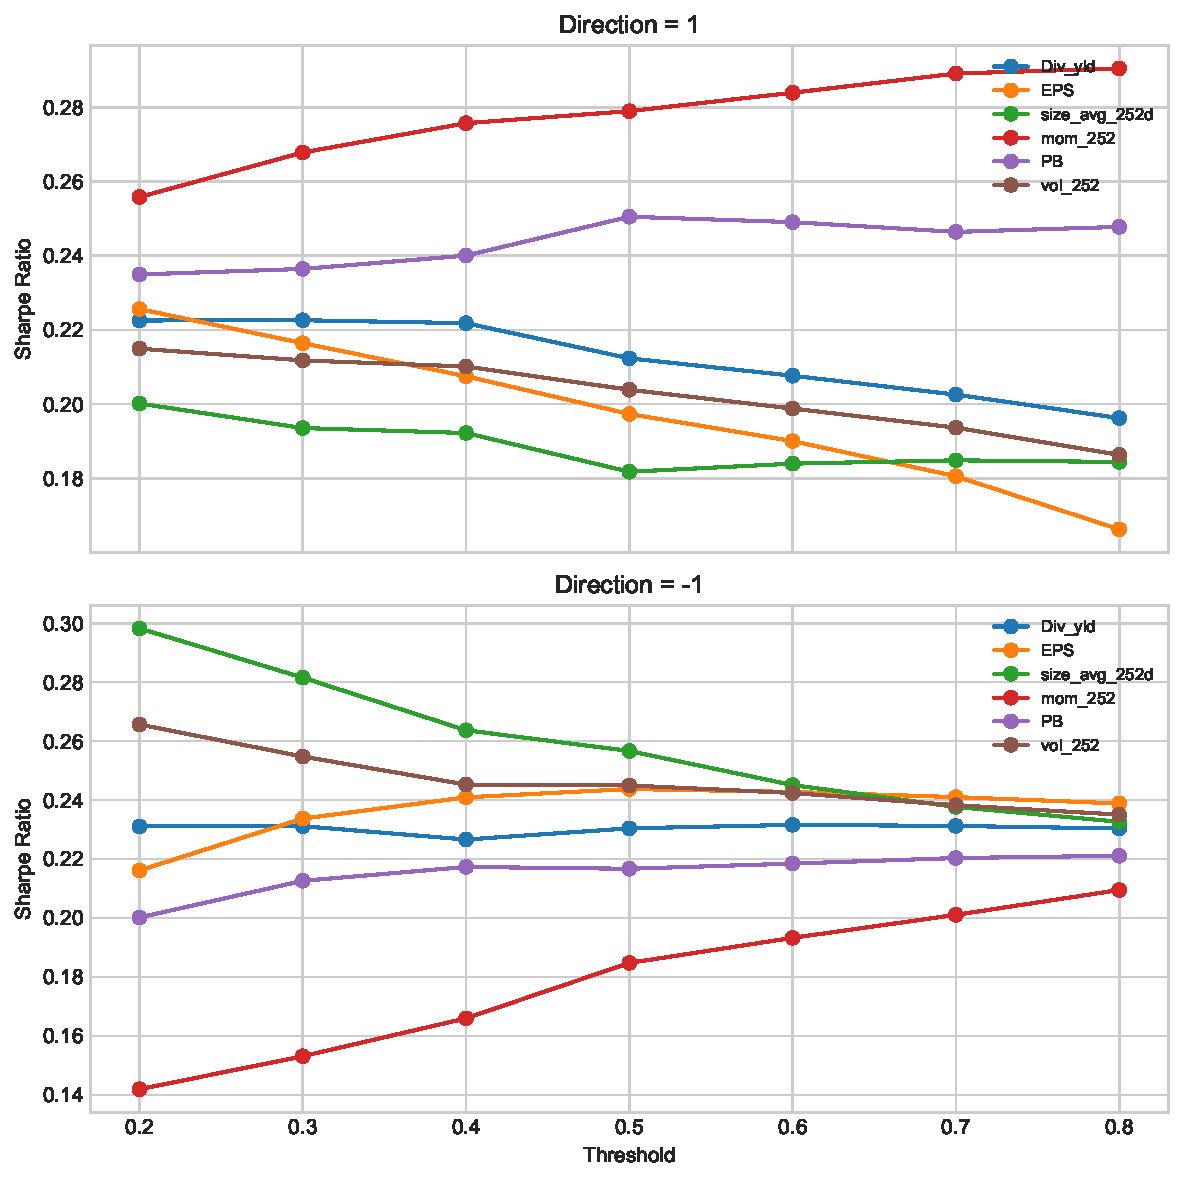
\includegraphics[width=0.7\linewidth]{files/0e8c8b7708bd7b7795d38bf77f2f91c6.pdf}}
\label{fig-backov_sr}
\end{figure}

The last step is to compute the statistic \ref{eq:tSR}. We code it here:

\begin{verbatim}
from scipy import stats as sp_stats
from scipy.special import digamma

def DSR(SR, Tt, M, g3, g4, SR_m, SR_v):
    """Compute Deflated Sharpe Ratio statistic."""
    gamma = -digamma(1)                                     # Euler-Mascheroni constant
    SR_star = SR_m + np.sqrt(SR_v) * (
        (1 - gamma) * sp_stats.norm.ppf(1 - 1/M) + 
        gamma * sp_stats.norm.ppf(1 - 1/(M * np.e))
    )                                                       # SR*
    num = (SR - SR_star) * np.sqrt(Tt - 1)                  # Numerator
    den = np.sqrt(1 - g3 * SR + (g4 - 1) / 4 * SR**2)       # Denominator
    return sp_stats.norm.cdf(num / den)
\end{verbatim}

All that remains to do is to evaluate the arguments of the function. The ``best'' strategy is the one with the highest Sharpe ratio and it is based on market capitalization.

\begin{verbatim}
M = len(pars)                                               # Number of strategies we tested
SR = grd['SR'].max()                                        # The SR we want to test
SR_m = grd['SR'].mean()                                     # Average SR across all strategies
SR_v = grd['SR'].var()                                      # Variance of SR

# Find the best strategy
best_idx = grd['SR'].idxmax()
best_feature = grd.loc[best_idx, 'feature']
best_thresh = grd.loc[best_idx, 'thresh']
best_direction = grd.loc[best_idx, 'direction']

print(f"Best strategy: feature={best_feature}, thresh={best_thresh}, direction={best_direction}")

# Compute returns of the best strategy
data_tmp = data_ml[['date', best_feature, 'R1M']].copy()
data_tmp['decision'] = (best_direction * data_tmp[best_feature] > best_direction * best_thresh)

returns_DSR = data_tmp.groupby('date').apply(
    lambda x: (x['decision'] / x['decision'].sum() * x['R1M']).sum()
              if x['decision'].sum() > 0 else 0
)

g3 = sp_stats.skew(returns_DSR)                             # Skewness
g4 = sp_stats.kurtosis(returns_DSR) + 3                     # Kurtosis
Tt = len(returns_DSR)                                       # Number of dates

dsr_value = DSR(SR, Tt, M, g3, g4, SR_m, SR_v)
print(f"Deflated Sharpe Ratio: {dsr_value:.4f}")
\end{verbatim}

\begin{verbatim}
Best strategy: feature=size_avg_252d, thresh=0.2, direction=-1
Deflated Sharpe Ratio: 0.4742
\end{verbatim}

The value is not high enough (it does not reach the 90\% or 95\% threshold) to make the strategy significantly superior to the other ones that were considered in the batch of tests.

\subsubsection{Coding exercises}

\begin{enumerate}
\item Code the returns of the EW portfolio with pandas functions only (no loop).
\item Code the advanced weighting function defined in Equation \ref{eq:coqw}.
\item Test it in a small backtest and check its sensitivity to the parameters.
\item Using parallelization (e.g., joblib), avoid the loop in the backtest.
\end{enumerate}

\subsection{Uncertainty quantification and conformal prediction}

Standard machine learning models produce point estimates. They offer no indication of reliability. An investor who knows a forecast is imprecise can reduce position sizes and avoid costly errors. Uncertainty quantification (UQ) addresses this gap. UQ attaches a measure of confidence to every prediction. It therefore transforms a raw signal into actionable information.

This chapter covers three traditions in UQ as applied to asset pricing. The first is conformal prediction, which delivers finite sample, distribution free coverage guarantees. The second is ambiguity aversion, which models investor behavior under Knightian uncertainty about the return generating process. The third is machine forecast disagreement, which treats dispersion across ML models as a proxy for hard to price risk. Together, these traditions offer a rich toolkit for practitioners who take model uncertainty seriously.

\subsubsection{Sources of prediction uncertainty}\label{sec_uncertainty_types}

Prediction uncertainty has two conceptually distinct sources. \textbf{Aleatoric} uncertainty is irreducible. It arises from idiosyncratic shocks that no model can eliminate regardless of sample size. In factor investing, idiosyncratic return variance is a canonical example. No amount of additional data removes it.

\textbf{Epistemic} uncertainty is reducible in principle. It stems from finite data and from limitations of the chosen model class. A model trained on few observations will disagree with a model trained on many. That disagreement shrinks as data accumulate. The two components call for different responses: aleatoric uncertainty should inform position sizing, while epistemic uncertainty motivates model averaging or Bayesian approaches.

Decomposing these components formally is not straightforward. \cite{ahdritz2024calibration} introduce higher order calibration to achieve this decomposition with formal guarantees. Their framework requires no distributional assumptions on the data generating process. It provides a provably valid separation between aleatoric and epistemic contributions to total prediction error.

\subsubsection{Conformal prediction}\label{sec_conformal}

Conformal prediction is a framework for constructing prediction intervals that carry a finite sample, distribution free coverage guarantee. Under exchangeability of the data, the coverage holds exactly regardless of the underlying distribution and regardless of the model used to generate predictions. The foundational theory is laid out in \cite{vovk2005algorithmic}. A concise and accessible introduction is provided by \cite{angelopoulos2023gentle}.

The key appeal in financial applications is the absence of parametric assumptions. Return distributions have heavy tails and change over time. Classical interval methods that assume normality are unreliable. Conformal methods sidestep this entirely. \cite{liao2025uncertainty} apply related ideas to asset pricing and show that neural network forecasts share an asymptotic distribution with nonparametric estimators, enabling closed form standard errors and bootstrap confidence intervals. They find that accounting for forecast uncertainty improves out of sample portfolio performance.

\paragraph{The split conformal algorithm}

The split conformal algorithm proceeds in three steps. First, the data are partitioned into a training set, a calibration set, and a test set. Second, a model $\hat{f}$ is fitted on the training set and used to predict on the calibration set. Third, nonconformity scores are computed, a quantile is derived from these scores, and intervals are formed for the test observations.

The coverage guarantee states that for a chosen miscoverage level $\alpha \in (0,1)$,

\begin{equation}
\label{eq_conformal_coverage}
P(y_{n+1} \in \hat{C}(x_{n+1})) \geq 1 - \alpha.
\end{equation}

The nonconformity score for calibration observation $i$ is the absolute residual of the model:

\begin{equation}
\label{eq_nonconformity}
s_i = |y_i - \hat{f}(x_i)|.
\end{equation}

The prediction interval for a new observation $x_{n+1}$ is then

\begin{equation}
\label{eq_conformal_interval}
\hat{C}(x_{n+1}) = [\hat{f}(x_{n+1}) - \hat{q},\; \hat{f}(x_{n+1}) + \hat{q}],
\end{equation}

where $\hat{q}$ is the $\lceil(n+1)(1 -\alpha)\rceil/n$ quantile of the calibration scores. This inflated quantile accounts for the finite size of the calibration set and is what delivers the guarantee in \ref{eq_conformal_coverage}. The interval is symmetric around the point prediction. It grows wider as $\alpha$ decreases (tighter coverage) and narrows as the calibration set grows.

The code below illustrates split conformal prediction on the book's US stock data. We use the seven standard characteristics from the dataset as predictors of next month returns. A ridge regression is trained on observations before 2013. The calibration set covers 2013 to 2016 and is used to derive the conformal quantile. The test set runs from 2017 onward.

\begin{verbatim}
import pandas as pd
import numpy as np
import matplotlib.pyplot as plt
import warnings
warnings.filterwarnings('ignore')

from sklearn.linear_model import Ridge
from sklearn.preprocessing import StandardScaler
from sklearn.neighbors import NearestNeighbors

pd.set_option('display.max_columns', 10)
plt.style.use('seaborn-v0_8-whitegrid')

from data_build import generate_data
data_ml, features, features_short, returns, stock_ids, stock_ids_short = generate_data()

cols_needed = ['date', 'fsym_id'] + features_short + ['R1M']
data_clean  = data_ml[cols_needed].dropna().copy()
data_clean['date'] = pd.to_datetime(data_clean['date'])
data_clean  = data_clean.sort_values('date').reset_index(drop=True)

print(f"Dataset: {len(data_clean):,} stock-month observations")
print(f"Date range: {data_clean['date'].min().date()} to {data_clean['date'].max().date()}")
print(f"Features: {features_short}")
\end{verbatim}

\begin{verbatim}
Dataset: 365,050 stock-month observations
Date range: 2002-01-31 to 2025-03-31
Features: ['Div_yld', 'EPS', 'size_avg_252d', 'mom_252', 'OCF_Growth_1Y', 'PB', 'vol_252']
\end{verbatim}

The dataset spans roughly 25 years of US stock returns. We reserve the most recent period for testing and use an intermediate window for calibration. This ordering matters: conformal prediction requires exchangeability, which is best approximated by keeping the splits chronological.

\begin{verbatim}
date_cal  = pd.Timestamp("2013-01-01")
date_test = pd.Timestamp("2017-01-01")

mask_train = data_clean['date'] < date_cal
mask_cal   = (data_clean['date'] >= date_cal) & (data_clean['date'] < date_test)
mask_test  = data_clean['date'] >= date_test

Xtr = data_clean.loc[mask_train, features_short].values
ytr = data_clean.loc[mask_train, 'R1M'].values
Xca = data_clean.loc[mask_cal,   features_short].values
yca = data_clean.loc[mask_cal,   'R1M'].values
Xte = data_clean.loc[mask_test,  features_short].values
yte = data_clean.loc[mask_test,  'R1M'].values

sc    = StandardScaler().fit(Xtr)
Xtr_s = sc.transform(Xtr)
Xca_s = sc.transform(Xca)
Xte_s = sc.transform(Xte)

mdl    = Ridge(alpha=1.0).fit(Xtr_s, ytr)
scores = np.abs(yca - mdl.predict(Xca_s))

alpha  = 0.10
n_ca   = len(scores)
q_hat  = np.quantile(scores, np.ceil((n_ca + 1) * (1 - alpha)) / n_ca)

ypred = mdl.predict(Xte_s)
lo    = ypred - q_hat
hi    = ypred + q_hat
cov   = np.mean((yte >= lo) & (yte <= hi))

print(f"Training obs   : {mask_train.sum():,}")
print(f"Calibration obs: {mask_cal.sum():,}")
print(f"Test obs       : {mask_test.sum():,}")
print(f"Conformal half-width: {q_hat:.4f}")
print(f"Target coverage    : {1 - alpha:.0%}")
print(f"Empirical coverage : {cov:.1%}")
\end{verbatim}

\begin{verbatim}
Training obs   : 161,873
Calibration obs: 66,675
Test obs       : 136,502
Conformal half-width: 0.1433
Target coverage    : 90%
Empirical coverage : 83.0%
\end{verbatim}

The conformal half width translates directly into an interval: any stock with a predicted return of $\hat{r}$ is assigned the interval $[\hat{r} - \hat{q},\, \hat{r} + \hat{q}]$. The empirical coverage on the test set should be at or above the 90\% target. We then estimate a local uncertainty for each test stock using the residuals of its nearest neighbors in the calibration set.

\begin{verbatim}
nn        = NearestNeighbors(n_neighbors=50).fit(Xca_s)
_, idx_nn = nn.kneighbors(Xte_s)
sigma_loc = np.array([scores[idx].std() for idx in idx_nn])

hi_ua = ypred + sigma_loc
lo_ua = ypred - sigma_loc

date_arr   = data_clean.loc[mask_test, 'date'].values
test_dates = sorted(data_clean.loc[mask_test, 'date'].unique())

ls_std_list, ls_ua_list = [], []

for dt in test_dates:
    mask_dt = date_arr == dt
    if mask_dt.sum() < 20:
        continue
    y_dt     = yte[mask_dt]
    pred_dt  = ypred[mask_dt]
    hi_dt    = hi_ua[mask_dt]
    lo_dt    = lo_ua[mask_dt]

    q10, q90 = np.percentile(pred_dt, [10, 90])
    ls_std   = y_dt[pred_dt >= q90].mean() - y_dt[pred_dt <= q10].mean()

    q10u, q90u = np.percentile(lo_dt, 10), np.percentile(hi_dt, 90)
    ls_ua      = y_dt[hi_dt >= q90u].mean() - y_dt[lo_dt <= q10u].mean()

    ls_std_list.append(ls_std)
    ls_ua_list.append(ls_ua)

ls_std_arr = np.array(ls_std_list)
ls_ua_arr  = np.array(ls_ua_list)

sr = lambda x: x.mean() / x.std() * np.sqrt(12)
print(f"Standard long short  — mean: {ls_std_arr.mean():.4f}, Sharpe: {sr(ls_std_arr):.2f}")
print(f"Uncertainty adjusted — mean: {ls_ua_arr.mean():.4f}, Sharpe: {sr(ls_ua_arr):.2f}")
\end{verbatim}

\begin{verbatim}
Standard long short  — mean: 0.0053, Sharpe: 0.27
Uncertainty adjusted — mean: 0.0011, Sharpe: 0.47
\end{verbatim}

Each month, stocks are ranked twice: once by point prediction and once by their uncertainty adjusted bounds. The Sharpe ratio comparison measures whether filtering on forecast precision adds value beyond the raw signal. Gains tend to be concentrated in months where cross sectional uncertainty is high.

\begin{verbatim}
import os
os.makedirs("images", exist_ok=True)

fig, axes = plt.subplots(1, 2, figsize=(12, 4))

# Left: cumulative long short returns
ax = axes[0]
dates_plot = [dt for dt, _ in zip(test_dates, ls_std_list)]
ax.plot(dates_plot, np.cumsum(ls_std_arr), color='steelblue', lw=1.5, label='Standard sort')
ax.plot(dates_plot, np.cumsum(ls_ua_arr),  color='firebrick', lw=1.5, label='Uncertainty adjusted')
ax.set_xlabel('Date')
ax.set_ylabel('Cumulative long short return')
ax.set_title('Portfolio performance (2017 onward)')
ax.legend()

# Right: empirical coverage by local uncertainty decile
nn_sub    = NearestNeighbors(n_neighbors=50).fit(Xca_s)
_, idx_ca = nn_sub.kneighbors(Xca_s)
sigma_ca  = np.array([scores[idx].std() for idx in idx_ca])

decile    = pd.qcut(sigma_ca, 10, labels=False)
pred_ca   = mdl.predict(Xca_s)
cov_dec   = []
for d in range(10):
    m   = decile == d
    cov_dec.append(np.mean((yca[m] >= pred_ca[m] - q_hat) & (yca[m] <= pred_ca[m] + q_hat)))

ax2 = axes[1]
ax2.bar(range(1, 11), cov_dec, color='steelblue', alpha=0.7)
ax2.axhline(1 - alpha, color='firebrick', linestyle='--', label=f'Target {1 - alpha:.0%}')
ax2.set_xlabel('Local uncertainty decile (low to high)')
ax2.set_ylabel('Empirical coverage')
ax2.set_title('Coverage by local uncertainty level')
ax2.legend()

plt.tight_layout()
plt.savefig('images/conformal_coverage.png', dpi=150, bbox_inches='tight')
plt.show()
\end{verbatim}

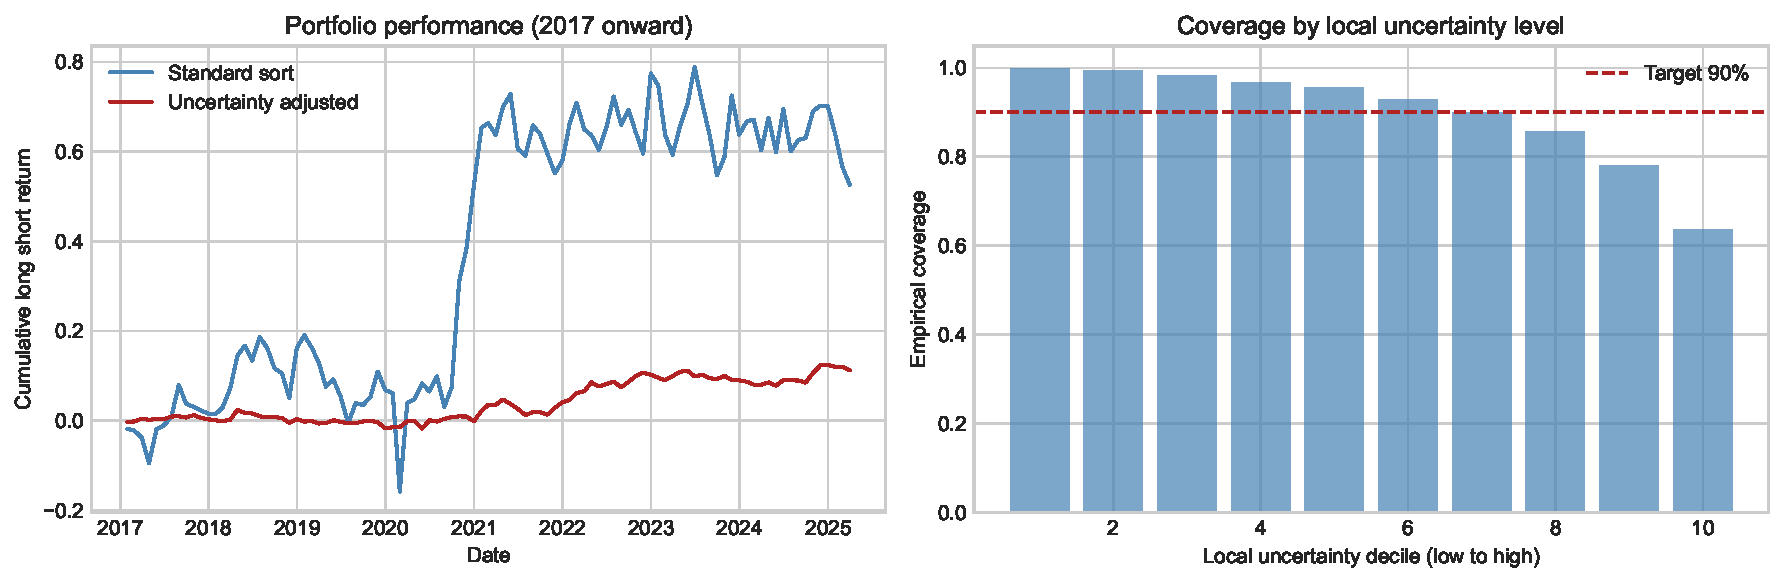
\includegraphics[width=0.7\linewidth]{files/3e3389da7ba18b1bfee206533660d199.pdf}

The left panel plots the cumulative returns of the two strategies over the test period. The right panel shows that empirical coverage is broadly uniform across local uncertainty deciles. This confirms the finite sample guarantee: regardless of how uncertain a prediction is, the conformal interval captures the true return at the specified rate.

\subsubsection{Uncertainty adjusted portfolio sorting}\label{sec_ua_sorting}

The standard approach in empirical asset pricing is to sort stocks on point predictions and form decile portfolios. The top decile goes long and the bottom decile goes short. This ignores the reliability of each prediction. A stock at the top of the predicted return distribution may have a very wide confidence interval. Its prediction could easily be wrong.

\cite{liu2026uncertainty} propose uncertainty adjusted sorting. Instead of ranking stocks on their point prediction $\hat{f}(x)$, investors go long on stocks with the highest upper prediction bounds and short on stocks with the lowest lower prediction bounds. This selects confident predictions. A stock enters the long leg only if its lower bound is also elevated. A stock enters the short leg only if its upper bound is also low.

The key empirical finding from \cite{liu2026uncertainty} is that performance gains relative to standard sorting come mainly from reduced portfolio volatility rather than from higher average returns. The mechanism is asset level uncertainty rather than aggregate market uncertainty. When individual stock uncertainty is high, the sorting procedure naturally avoids those stocks, reducing idiosyncratic risk in the portfolio.

\cite{allena2025confident} reaches similar conclusions from a different angle. He derives ex ante confidence intervals from linear and ML models including Lasso, Elastic Net, Ridge and neural networks. Confident high low strategies, which trade only on stocks with precise forecasts, systematically outperform their standard counterparts. The result holds across all model classes. This convergence of evidence across methods suggests that incorporating forecast precision into portfolio construction is a robust improvement over point prediction sorting.

\subsubsection{Machine forecast disagreement}\label{sec_mfd}

\cite{bali2025disagreement} introduce the concept of machine forecast disagreement (MFD). The idea draws on the classical analyst disagreement literature but replaces human analysts with ML model specifications. Different model architectures, different hyperparameters, and different feature sets produce different return forecasts for the same stock. The dispersion of these forecasts measures how much the ``ML crowd'' disagrees about a stock's prospects.

The analogy with investor disagreement is natural. In models with short sale constraints, disagreement among investors leads to overpricing because the most optimistic investors set prices while pessimists cannot easily arbitrage. The same logic applies here. Stocks with high MFD are harder to price, harder to arbitrage, and consequently overpriced.

Empirically, \cite{bali2025disagreement} find that stocks in the highest MFD decile earn returns roughly 14\% per year lower than stocks in the lowest MFD decile on a value weighted basis. This spread is robust to standard risk controls. MFD also outperforms traditional analyst forecast dispersion measures in predicting cross sectional returns. The reason is that ML models cover the full cross section of stocks including those with no analyst coverage, and they do so at high frequency with consistent methodology.

The connection to limits to arbitrage is important. High MFD stocks tend to be small, illiquid, and costly to short. The same frictions that prevent arbitrageurs from correcting overpricing are correlated with the conditions that generate high ML disagreement. MFD therefore acts as a joint measure of uncertainty and arbitrage difficulty.

\subsubsection{Ambiguity aversion and portfolio choice}\label{sec_ambiguity}

Knight distinguished risk, where probabilities are known, from ambiguity, where they are not. ML models introduce a specific form of ambiguity: different plausible models of the return generating process produce different optimal portfolios. \cite{ghysels2022ambiguity} quantify this ML ambiguity via bootstrap resampling. Each bootstrap resample yields a different trained model and hence a different forecast. The spread across resamples separately captures upside and downside scenarios, a concept the authors term directional uncertainty. Investors who internalize this ambiguity by adopting pessimistic positions where disagreement is high achieve better Sharpe ratios than those who rely on a single model estimate.

\cite{hara2022ambiguity} provide a theoretical foundation for thinking about implied ambiguity. They derive a one to one mapping between the degree of implied ambiguity inferred from portfolio inefficiency, the observed Sharpe ratio, and pricing errors in the cross section. The result holds under a smooth ambiguity model where the representative investor has preferences over both risk and ambiguity. Calibrating the model to US data, they find significant ambiguity aversion. This suggests that the equity premium itself reflects compensation not only for risk but for Knightian uncertainty about model parameters.

\cite{bianchi2026uncertainty} take a Bayesian neural network (BNN) approach to the same problem. Rather than mapping characteristics to expected returns, BNNs map firm characteristics directly to portfolio weights by maximizing expected utility under the posterior distribution over network parameters. The posterior induces a distribution over optimal weights. Averaging over this distribution yields more stable allocations than point estimates from standard deep learning. No trade regions arise naturally because the posterior uncertainty about a stock's weight may be so large that no position is justified. Posterior sparsity further reduces turnover. The resulting strategy outperforms linear models and standard neural networks, particularly after transaction costs, suggesting that parameter uncertainty is economically significant.

\subsubsection{Time varying uncertainty and signal selection}\label{sec_timevarying_unc}

The optimal weighting of predictive signals changes over time. During periods of high economic uncertainty, short term signals become noisier while long term structural relationships remain more stable. \cite{chen2026uncertainty} formalize this intuition with U-LASSO, an adaptive penalization scheme that mixes long term and short term predictive signals based on the current level of economic uncertainty.

The mechanism operates through two distinct channels. The noisy signal channel, driven by real and financial uncertainty, pushes investors toward stable long term signals. These signals are less affected by transient shocks and provide more reliable forecasts when the environment is volatile. The volatile state channel, driven by macro uncertainty and the VIX, pushes investors toward short term signals because the economy is changing rapidly enough that long term averages become stale.

\cite{chen2026uncertainty} show that economic uncertainty explains nearly 30\% of the variation in the optimal signal horizon weight. This is a large share of explained variation for a single variable and underlines the economic importance of the uncertainty regime. U-LASSO outperforms both traditional penalized regressions and standard ML benchmarks in out of sample portfolio performance. The result holds across different uncertainty measures and subperiods, suggesting robustness beyond any particular calibration choice.

\subsubsection{Uncertainty in large language model predictions}\label{sec_llm_unc}

Large language models (LLMs) are increasingly used to classify financial text and generate investment signals. However, standard LLM outputs come with no natural measure of confidence. The model simply returns a predicted label or score. \cite{chen2026llm} address this gap by constructing an entropy measure from the inner conditional probabilities over possible outputs rather than from the generated text itself.

The approach exploits the token level probability distributions that LLMs compute internally. High entropy means the model is uncertain about which output to generate. Low entropy means the model assigns high probability to one particular output. Crucially, this inner probability differs from the confidence that some models report in their generated text. Decoding biases cause models to express false certainty in their generated language even when their internal distributions are diffuse. The entropy measure bypasses this problem.

\cite{chen2026llm} show that high confidence predictions (low entropy) are systematically more accurate in financial text classification tasks. A portfolio built on high confidence LLM signals achieves a Sharpe ratio approximately 20\% above the benchmark. Low confidence predictions contribute no excess return. This finding implies that filtering LLM signals by their internal uncertainty is a meaningful source of alpha, and that practitioners should not rely on LLM self assessment to determine when to trust the model.

\subsubsection{Exercises}

\begin{enumerate}
\item Using the simulated data above, vary the miscoverage level alpha from 0.05 to 0.30. Plot the empirical coverage and interval width as a function of alpha. Does the finite sample guarantee hold throughout?
\item Replace the ridge regression with a gradient boosting model. Recompute the conformal quantile and assess whether empirical coverage is maintained.
\item Implement an asymmetric conformal interval where the long leg uses the upper bound $\hat{f}(x) + \hat{q}$ and the short leg uses the lower bound $\hat{f}(x) - \hat{q}$. Compare the resulting portfolio with the uncertainty adjusted sort described in the chapter.
\item Simulate machine forecast disagreement by fitting five ridge regressions on different bootstrap samples of the training data. Compute the dispersion of predictions and test whether high disagreement stocks earn lower simulated returns.
\item Discuss conceptually how the U-LASSO of \cite{chen2026uncertainty} could be implemented in a panel regression setting. What observable variable would you use as the uncertainty measure, and how would it enter the penalization scheme?
\end{enumerate}

\subsection{Design uncertainty and nonstandard errors}

Every empirical result is the endpoint of a long chain of decisions. Which firms enter the sample? How are missing values handled? Where is the sorting threshold placed? How are portfolio positions weighted? None of these questions has a single defensible answer. Each one is a fork, and each fork multiplies the number of studies that could have been written from the same data.

The previous chapter treated uncertainty that comes from the data. This chapter treats uncertainty that comes from the analyst. The two are distinct. Sampling noise shrinks as observations accumulate, while the dispersion caused by methodological choices does not. A larger dataset does not tell you where to place a quantile cutoff.

We first formalize a research protocol as a sequence of choices, following \cite{coqueret2026persistent}. We then define the \textbf{nonstandard error}, introduced by \cite{menkveld2021standard}, and show how it can be separated from the standard error within a single variance decomposition. We close with a worked example on the value premium, where three simple choices generate eighteen defensible estimates of the same quantity.

\subsubsection{The garden of forking paths}\label{sec_design_forks}

\cite{gelman2014statistical} describe the \textbf{garden of forking paths}: a researcher who analyzes a dataset makes many decisions that are contingent on the data, and the resulting result is one draw from a space of results that were never reported. The problem is not dishonesty. An analyst who runs a single specification and reports it faithfully still hides the variability that the unreported specifications would have revealed.

Two experimental designs have been used to map this space. In a \textbf{multi analyst study}, independent teams receive the same data and the same question. \cite{silberzahn2018many} gave 29 teams one dataset and asked whether soccer referees give more red cards to dark skinned players. The estimated effects ranged from no effect to a large one. \cite{botviniknezer2020} repeated the exercise on a neuroimaging dataset with 70 teams and found that no two teams used the same analysis pipeline. \cite{huntington2021influence} document the same dispersion in applied microeconomics.

In a \textbf{multi path study}, a single team enumerates the choices explicitly and runs all of the combinations. \cite{simonsohn2020specification} call the resulting object a specification curve. In finance, \cite{mitton2021methodological} spans 1,024 paths in corporate finance, \cite{soebhag2022mind} and \cite{walter2022non} do so for portfolio sorts, \cite{fieberg2024non} for cryptocurrencies, and \cite{battistella2025multiverse} and \cite{cakici2025lost} across asset classes. The example in this chapter is a small multi path study.

\paragraph{A protocol as a sequence of choices}

Following \cite{coqueret2026persistent}, we model an empirical study as a composition of operations applied to a dataset $\mathbb{D}$. If the protocol has $J$ steps, the reported result is

\begin{equation}
\label{eq_design_path}
\hat{b} := \hat{b}(\mathbb{D}) = f_J \circ f_{J-1} \circ \dots \circ f_1(\mathbb{D}),
\end{equation}

where $\hat{b}$ is the object of interest. It may be an average return, a $t$ statistic, or an alpha. Each step $f_j$ offers $r_j \ge 2$ defensible options, so the number of distinct \textbf{paths} is

\begin{equation}
\label{eq_design_count}
P = \prod_{j=1}^J r_j.
\end{equation}

The multiplicative form is what makes this a practical concern. Seven binary or ternary choices already generate several hundred paths. \cite{coqueret2026persistent} use seven forks and obtain $P = 576$; \cite{walter2022non} use fourteen and obtain 69,120. Since each path yields its own estimate, we index outcomes by the path and write $\hat{b}_p$ for $p = 1, \dots, P$.

Two properties of this notation matter. First, $\hat{b}_p$ is random because $\mathbb{D}$ is random, so each path has a sampling distribution. Second, two paths that share many steps will produce similar answers on the same data. Both properties reappear below.

\subsubsection{Standard and nonstandard errors}\label{sec_design_nse}

\cite{menkveld2021standard} coined the term \textbf{nonstandard error} for the dispersion in results that is attributable to the choices of the analyst rather than to the data. Their multi analyst study of market microstructure found these errors to be sizable, and comparable in magnitude to the standard errors that researchers habitually report.

The literature measures the nonstandard error either as the interquartile range of outcomes across paths (\cite{menkveld2021standard}, \cite{walter2022non}) or as their cross sectional standard deviation (\cite{soebhag2022mind}, \cite{fieberg2024non}). The standard error is measured separately, usually by bootstrapping the returns of each path after the paths have been run. The two quantities are therefore built on different reference objects and do not combine into anything.

\cite{coqueret2026persistent} close this gap. Suppose the analyst runs every path on several samples, so that each outcome $\hat{b}_p(\mathbb{D})$ is indexed by both a path $p$ and a sample $\mathbb{D}$. The law of total variance (see chapter 9 of \cite{blitzstein2019introduction}) can then be applied twice to the same quantity $\sigma_b^2 = \mathbb{V}[\hat{b}_p(\mathbb{D})]$. Conditioning on the sample gives

\begin{equation}
\label{eq_design_ltv_sample}
\sigma_b^2 = \mathbb{V}\big[\mathbb{E}[\hat{b}\,|\,\mathbb{D}]\big] + \mathbb{E}\big[\mathbb{V}[\hat{b}\,|\,\mathbb{D}]\big],
\end{equation}

where the second term is the variance across paths within a sample, averaged over samples. That is the nonstandard error of the literature, with the refinement that it is averaged rather than computed on a single dataset. Conditioning on the path instead gives

\begin{equation}
\label{eq_design_ltv_path}
\sigma_b^2 = \mathbb{V}\big[\mathbb{E}[\hat{b}\,|\,p]\big] + \mathbb{E}\big[\mathbb{V}[\hat{b}\,|\,p]\big],
\end{equation}

where the second term is the variance across samples within a path, averaged over paths. That is the standard error of the literature.

Both identities are valid and neither is preferable, so \cite{coqueret2026persistent} take one half of each pair:

\begin{equation}
\label{eq_design_se}
\text{SE} = \sqrt{\frac{\mathbb{E}\big[\mathbb{V}[\hat{b}\,|\,p]\big] + \mathbb{V}\big[\mathbb{E}[\hat{b}\,|\,\mathbb{D}]\big]}{2}},
\end{equation}

\begin{equation}
\label{eq_design_nse}
\text{NSE} = \sqrt{\frac{\mathbb{V}\big[\mathbb{E}[\hat{b}\,|\,p]\big] + \mathbb{E}\big[\mathbb{V}[\hat{b}\,|\,\mathbb{D}]\big]}{2}}.
\end{equation}

Adding \ref{eq_design_ltv_sample} and \ref{eq_design_ltv_path} and dividing by two shows that these definitions satisfy

\begin{equation}
\label{eq_design_sum}
\sigma_b^2 = \text{SE}^2 + \text{NSE}^2.
\end{equation}

This is the appeal of the construction. The two errors are now shares of one budget, so the statement that methodological uncertainty dominates sampling uncertainty becomes a statement about a decomposition rather than a comparison of two unrelated numbers. We verify \ref{eq_design_sum} numerically below.

\subsubsection{Why correlation across paths matters}\label{sec_design_corr}

Having many estimates is only useful if they carry independent information. Let $\hat{\mu}_b = P^{ -1}\sum_p \hat{b}_p$ be the average outcome across paths. Its variance is not $\sigma_b^2 / P$, because the outcomes are not independent:

\begin{equation}
\label{eq_design_varmean}
\sigma^2_{\hat{\mu}_b} = \frac{\sigma_b^2}{P^2}\sum_{1 \le p,q \le P} \rho_{p,q},
\qquad \rho_{p,q} = \mathbb{C}\text{or}\big(\hat{b}_p(\mathbb{D}), \hat{b}_q(\mathbb{D})\big).
\end{equation}

Combining \ref{eq_design_varmean} with \ref{eq_design_sum} gives the canonical expression

\begin{equation}
\label{eq_design_canonical}
\sigma^2_{\hat{\mu}_b} = \big(\text{SE}^2 + \text{NSE}^2\big) \sum_{p,q} \frac{\rho_{p,q}}{P^2}.
\end{equation}

Three quantities therefore drive the width of any confidence interval around the mean effect: the standard error, the nonstandard error, and the average correlation across paths. If the correlations were all zero, the last term would collapse to $1/P$ and adding paths would sharpen inference. If the correlations are close to one, the term stays close to one and the $P$ paths deliver no more information than a single one.

It may seem paradoxical that agreement across paths is undesirable. The resolution is that each path is a separate model learning from the data. Ideally all of them reach the same conclusion, but for different reasons. Agreement that emerges from different perspectives is evidence of robustness. Agreement that emerges because the paths are looking at the same rows of the same table is not. The same intuition underlies bagging and random forests, where the benefit of an ensemble comes from decorrelating its members (\cite{breiman2001random}), a point developed in Chapter \href{/chap-14-ensemble}{Ensemble models}.

This suggests an operational fix. Analysts normally run every path on one fixed dataset, which we call \textbf{common resampling} when the exercise is repeated on perturbed versions of that dataset. \cite{coqueret2026persistent} instead recommend \textbf{path specific resampling}: draw a fresh sample immediately before running each path. The paths then no longer share their sampling noise, the correlations collapse toward zero, and the sum in \ref{eq_design_canonical} falls to roughly $1/P$. In their study of 107 anomalies, the average correlation falls from about 0.17 to essentially zero, which narrows the confidence interval for the mean by a factor of about five.

\subsubsection{The nonstandard Sharpe ratio}\label{sec_design_nsr}

If the nonstandard error measures how much an estimate moves when the protocol moves, then a return should be judged against it. \cite{coqueret2026persistent} define the \textbf{nonstandard Sharpe ratio} as the mean outcome scaled by the nonstandard error:

\begin{equation}
\label{eq_design_nsr}
\text{NSR} = \frac{\bar{r}}{\text{NSE}}, \qquad \bar{r} = \sum_{p=1}^P \omega_p r_p,
\end{equation}

where $r_p$ is the average return of the portfolio built along path $p$ and the $\omega_p$ are weights that sum to one. Uniform weights $\omega_p = 1/P$ treat all paths as equally defensible. Unequal weights let the analyst favor the conventional specification and downweight exotic ones.

When each path is run once and correlations can be assumed away, the nonstandard error is simply the dispersion of outcomes across paths and the ratio becomes

\begin{equation}
\label{eq_design_nsr_simple}
\text{NSR} = \frac{\bar{r}}{\sqrt{\sum_{p=1}^P \omega_p (r_p - \bar{r})^2}}.
\end{equation}

The interpretation parallels the Sharpe ratio, with cross path dispersion replacing time series volatility. A factor with a large average return can still have a low nonstandard Sharpe ratio if its performance depends on how it is built. Up to a scaling constant, the NSR is the $t$ statistic for testing whether the mean across paths differs from zero, so it doubles as a decision rule. \cite{coqueret2026persistent} call an anomaly \textbf{persistent} when it survives both sampling noise and methodological variation, and they find that persistence is determined almost entirely by the NSR, with a threshold near one. Of the 107 anomalies they examine, 26 are persistent under every configuration they test.

\subsubsection{A worked example: the value premium}\label{sec_design_value}

\cite{asness2013devil} is the natural illustration. Their title, the devil in HML's details, refers to the fact that the value factor of \cite{fama1993common} is defined with annually updated book values matched to lagged prices, and that seemingly innocuous departures from that convention change the measured premium substantially. Value is a good test case precisely because the underlying idea, that cheap stocks outperform expensive ones, is simple and uncontested. Whatever dispersion we find comes from implementation, not from disagreement about the hypothesis.

We keep three forks, each with an obvious menu of options:

\begin{itemize}
\item \textbf{Sorting quantile}: the tails used for the two legs, at 10\%, 20\% or 30\%. \cite{chen2021open} document that published studies mostly use quintiles or deciles, with no consensus.
\item \textbf{Size filter}: whether the smallest firms are removed, and how many. We try no filter, dropping the smallest 5\%, and dropping the smallest 10\%. Small firms are illiquid and expensive to trade, and they dominate equally weighted portfolios.
\item \textbf{Weighting}: equal weights or capitalization weights. \cite{plyakha2021equal} show that this choice alone changes the conclusion of asset pricing tests.
\end{itemize}

That gives $3 \times 3 \times 2 = 18$ designs. This is a deliberately small design space, so it runs in under a minute; the studies cited above span hundreds or thousands of paths.

\begin{verbatim}
# Required libraries
import itertools
import numpy as np
import pandas as pd
import matplotlib.pyplot as plt
from matplotlib.lines import Line2D
import warnings
warnings.filterwarnings('ignore')

plt.style.use('seaborn-v0_8-whitegrid')

from data_build import generate_data
data_ml, features, features_short, returns, stock_ids, stock_ids_short = generate_data()

# The characteristics of the book are uniformized cross-sectionally: each one is
# a rank in [0,1], recomputed every month. A low price-to-book rank flags a value
# stock, so the book-to-market rank is one minus the PB rank. Likewise, the size
# rank stands in for market capitalization.
panel = pd.DataFrame({
    'date': data_ml['date'].values,
    'bm':   1 - data_ml['PB'].values,           # book-to-market rank
    'size': data_ml['size_avg_252d'].values,    # capitalization rank
    'ret':  data_ml['R1M'].values,              # one month forward return
})

print(f"Observations : {len(panel):,}")
print(f"Months       : {panel['date'].nunique()}")
print(f"Stocks       : {data_ml['fsym_id'].nunique():,}")
print(f"Period       : {panel['date'].min().date()} to {panel['date'].max().date()}")
\end{verbatim}

\begin{verbatim}
Observations : 365,050
Months       : 279
Stocks       : 1,950
Period       : 2002-01-31 to 2025-03-31
\end{verbatim}

Because the ranks are uniform within each month, the two design steps are easy to express. A size floor of 0.05 removes exactly the smallest 5\% of firms in every cross section. A sorting quantile of 0.10 puts the cheapest tenth in the long leg and the most expensive tenth in the short leg. The function below implements one design; the second function runs all eighteen and reuses the ranking, which depends on the size filter but not on the other two choices.

\begin{verbatim}
QUANTILES = [0.10, 0.20, 0.30]     # tails used for the long and short legs
FLOORS    = [0.00, 0.05, 0.10]     # share of the smallest firms removed
WEIGHTS   = ['EW', 'CW']           # equal versus capitalization weighted

DESIGNS = list(itertools.product(QUANTILES, FLOORS, WEIGHTS))
print(f"Forks: 3, paths: {len(DESIGNS)}")


def long_short(df, quantile, floor, weighting):
    """Monthly return series of the long-short portfolio of one design."""
    kept = df[df['size'] > floor]
    rank = kept.groupby('date')['bm'].rank(pct=True).values
    dates, ret, size = kept['date'].values, kept['ret'].values, kept['size'].values
    w = np.ones(len(kept)) if weighting == 'EW' else size

    legs = []
    for leg in (rank >= 1 - quantile, rank <= quantile):
        agg = pd.DataFrame({'date': dates[leg],
                            'num': (ret * w)[leg],
                            'den': w[leg]}).groupby('date').sum()
        legs.append(agg['num'] / agg['den'])
    return legs[0] - legs[1]


def all_designs(df):
    """Average long-short return of all 18 designs, on one sample."""
    out = {}
    for floor in FLOORS:
        kept = df[df['size'] > floor]
        rank = kept.groupby('date')['bm'].rank(pct=True).values
        dates, ret, size = kept['date'].values, kept['ret'].values, kept['size'].values
        for quantile in QUANTILES:
            top, bottom = rank >= 1 - quantile, rank <= quantile
            for weighting in WEIGHTS:
                w = np.ones(len(kept)) if weighting == 'EW' else size
                legs = []
                for leg in (top, bottom):
                    agg = pd.DataFrame({'date': dates[leg],
                                        'num': (ret * w)[leg],
                                        'den': w[leg]}).groupby('date').sum()
                    legs.append(agg['num'] / agg['den'])
                out[(quantile, floor, weighting)] = (legs[0] - legs[1]).mean()
    return out
\end{verbatim}

\begin{verbatim}
Forks: 3, paths: 18
\end{verbatim}

We now run the eighteen designs on the full sample. Returns are expressed in percent per month.

\begin{verbatim}
baseline = all_designs(panel)
b_full = np.array([baseline[d] for d in DESIGNS]) * 100

table = pd.DataFrame(DESIGNS, columns=['Quantile', 'Size floor', 'Weighting'])
table['Avg. return (%)'] = b_full.round(4)
table = table.sort_values('Avg. return (%)', ascending=False).reset_index(drop=True)
print(table.to_string(index=False))

print(f"\nmean {b_full.mean():.4f}   min {b_full.min():.4f}   "
      f"max {b_full.max():.4f}   ratio {b_full.max() / b_full.min():.1f}")
\end{verbatim}

\begin{verbatim}
Quantile  Size floor Weighting  Avg. return (%)
      0.2        0.00        CW           0.1749
      0.3        0.00        CW           0.1668
      0.3        0.05        EW           0.1654
      0.2        0.05        EW           0.1640
      0.2        0.10        EW           0.1620
      0.2        0.00        EW           0.1619
      0.3        0.10        EW           0.1608
      0.1        0.05        CW           0.1592
      0.2        0.05        CW           0.1565
      0.1        0.10        EW           0.1561
      0.3        0.05        CW           0.1561
      0.3        0.00        EW           0.1474
      0.2        0.10        CW           0.1470
      0.1        0.05        EW           0.1459
      0.3        0.10        CW           0.1436
      0.1        0.10        CW           0.1433
      0.1        0.00        CW           0.1412
      0.1        0.00        EW           0.0625

mean 0.1508   min 0.0625   max 0.1749   ratio 2.8
\end{verbatim}

Every design produces a positive premium, so the sign of the effect is not in question. The magnitude is. The largest estimate is roughly 2.8 times the smallest, and the weakest design by a wide margin is the one that sorts on the extreme deciles, applies no size filter, and weights equally. This is the configuration in which the long leg loads most heavily on tiny illiquid firms, and it is exactly the sensitivity that \cite{asness2013devil} emphasize. An analyst who reported only that path, and an analyst who reported only the strongest path, would both be reporting a defensible number.

\begin{verbatim}
order  = np.argsort(b_full)
labels = [f"{d[0]:.0%} / {d[1]:.0%} / {d[2]}" for d in DESIGNS]
colors = ['steelblue' if d[2] == 'EW' else 'firebrick' for d in DESIGNS]

# The printed page reduces every figure, so the canvas is kept narrow and the
# type large. What looks oversized on screen is what stays readable in print.
fig, ax = plt.subplots(figsize=(6.5, 5.5))
ax.hlines(range(18), 0, b_full[order], color=[colors[i] for i in order], lw=1.2, alpha=0.5)
ax.scatter(b_full[order], range(18), c=[colors[i] for i in order], s=55, zorder=3)
ax.axvline(b_full.mean(), color='black', linestyle='--', lw=1.2)

ax.set_yticks(range(18))
ax.set_yticklabels([labels[i] for i in order], fontsize=11)
ax.tick_params(axis='x', labelsize=11)
ax.set_xlabel('Average monthly long short return (%)', fontsize=12)
ax.set_ylabel('quantile / size floor / weighting', fontsize=12)
ax.set_title('The value premium under 18 designs', fontsize=13)
ax.set_xlim(0, b_full.max() * 1.45)
ax.legend(handles=[Line2D([], [], marker='o', ls='', color='steelblue', label='Equally weighted'),
                   Line2D([], [], marker='o', ls='', color='firebrick', label='Cap weighted'),
                   Line2D([], [], ls='--', color='black', label='Mean across designs')],
          loc='lower right', fontsize=10)
plt.tight_layout()
plt.show()
\end{verbatim}

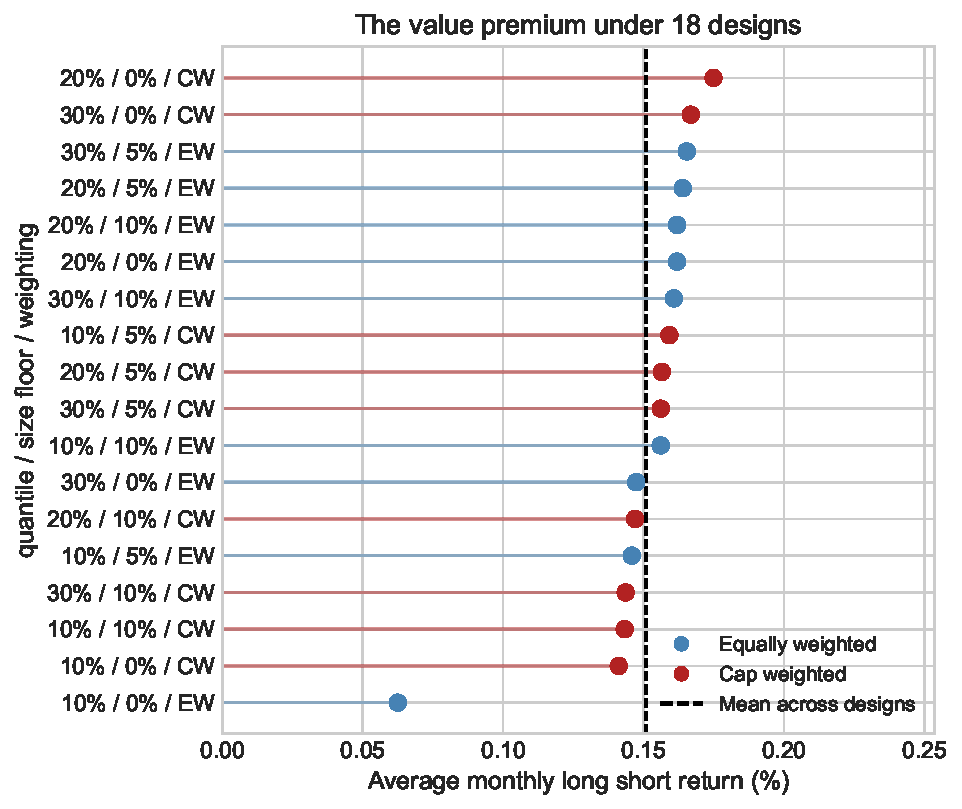
\includegraphics[width=0.7\linewidth]{files/1a7fe655332a1ac1304f014838fcc4a6.pdf}

\paragraph{Resampling and the correlation across paths}

We now repeat the exercise on perturbed versions of the data. Each sample is a random 40\% of the stock month observations, drawn without replacement. Under \textbf{common resampling} one sample is drawn and all eighteen designs are run on it. Under \textbf{path specific resampling} a fresh sample is drawn immediately before each design. The two schemes differ only in the order of two lines, but that order determines whether the paths share their sampling noise.

\begin{verbatim}
rng       = np.random.default_rng(42)
N_SAMPLES = 50
FRACTION  = 0.40
n_rows    = len(panel)
n_draw    = int(FRACTION * n_rows)


def subsample():
    """A random 40% of the stock month observations, without replacement."""
    return panel.iloc[np.sort(rng.choice(n_rows, size=n_draw, replace=False))]


# Common resampling: draw one sample, then run every design on it.
rows = []
for _ in range(N_SAMPLES):
    outcome = all_designs(subsample())
    rows.append([outcome[d] for d in DESIGNS])
common = np.array(rows) * 100

# Path specific resampling: draw a new sample before each design.
specific = np.empty((N_SAMPLES, len(DESIGNS)))
for i in range(N_SAMPLES):
    for j, (quantile, floor, weighting) in enumerate(DESIGNS):
        specific[i, j] = long_short(subsample(), quantile, floor, weighting).mean() * 100

print(f"Outcome matrices: {common.shape} (samples x paths)")


def average_correlation(M):
    """Average of the off-diagonal correlations across paths."""
    C = np.corrcoef(M, rowvar=False)
    P = C.shape[0]
    return (C.sum() - np.trace(C)) / (P * (P - 1)), C


rho_common, C_common = average_correlation(common)
rho_spec,   C_spec   = average_correlation(specific)

print(f"Average correlation, common resampling   : {rho_common:+.3f}")
print(f"Average correlation, path specific       : {rho_spec:+.3f}")
\end{verbatim}

\begin{verbatim}
Outcome matrices: (50, 18) (samples x paths)
Average correlation, common resampling   : +0.689
Average correlation, path specific       : -0.010
\end{verbatim}

The contrast is stark. Sharing a sample across designs induces an average correlation near 0.69, while drawing a separate sample for each design brings it to zero. Recall from \ref{eq_design_canonical} that the relevant quantity is $\sum_{p,q}\rho_{p,q}/P^2$, which equals $1/P + (1 - 1/P)\bar{\rho}$ when the correlations are homogeneous. With $P = 18$ this is about 0.71 under common resampling and about 0.05 under path specific resampling, a difference of more than a factor of ten in the variance of the mean.

We now apply the decomposition of \ref{eq_design_se} and \ref{eq_design_nse}. Because the outcomes form a balanced grid of samples by paths, the population variances (with \texttt{ddof=0}) satisfy the additivity of \ref{eq_design_sum} exactly, which the code checks.

\begin{verbatim}
def decompose(M):
    """Split the variance of the effect into a standard and a nonstandard error."""
    v_across_paths   = M.var(axis=1, ddof=0).mean()   # E[V[b | D]]
    v_of_sample_mean = M.mean(axis=1).var(ddof=0)     # V[E[b | D]]
    v_across_samples = M.var(axis=0, ddof=0).mean()   # E[V[b | p]]
    v_of_path_mean   = M.mean(axis=0).var(ddof=0)     # V[E[b | p]]
    se  = np.sqrt((v_across_samples + v_of_sample_mean) / 2)
    nse = np.sqrt((v_of_path_mean + v_across_paths) / 2)
    return se, nse


for name, M, rho in [('common', common, rho_common),
                     ('path specific', specific, rho_spec)]:
    se, nse = decompose(M)
    P = M.shape[1]
    corr_term = 1 / P + (1 - 1 / P) * rho          # sum of rho_pq divided by P^2
    sigma_mu  = np.sqrt((se ** 2 + nse ** 2) * corr_term)
    print(f"{name:14s} SE {se:.4f}  NSE {nse:.4f}  "
          f"SE2+NSE2 {se ** 2 + nse ** 2:.6f} vs total variance {M.var(ddof=0):.6f}")
    print(f"{'':14s} correlation term {corr_term:.3f}  "
          f"standard deviation of the mean {sigma_mu:.4f}")
\end{verbatim}

\begin{verbatim}
common         SE 0.0602  NSE 0.0333  SE2+NSE2 0.004735 vs total variance 0.004735
               correlation term 0.706  standard deviation of the mean 0.0578
path specific  SE 0.0581  NSE 0.0569  SE2+NSE2 0.006608 vs total variance 0.006608
               correlation term 0.046  standard deviation of the mean 0.0174
\end{verbatim}

The additivity of \ref{eq_design_sum} holds to the last digit, as it must. The economically relevant line is the last one: the standard deviation of the mean effect falls from about 0.058 to about 0.017 when resampling is done path by path. The estimate of the average premium is unchanged, but the precision with which we know it improves by a factor of more than three.

Note also that the standard error and the nonstandard error are of comparable size here. That is a consequence of the small design space. With only three forks the paths are close relatives of one another, so their dispersion is limited, while a 40\% subsample injects a substantial amount of sampling noise. \cite{coqueret2026persistent} span 576 paths and find the nonstandard error to be an order of magnitude larger than the standard error for most anomalies. The nonstandard error grows with the number of forks, so a study that enumerates more choices will attribute more of its total variance to methodology.

\begin{verbatim}
iu = np.triu_indices(18, k=1)

# Two stacked panels rather than two side by side: each one then keeps the full
# width of the figure, which survives the reduction applied on the printed page.
fig, axes = plt.subplots(2, 1, figsize=(6.5, 7.5))

# Top: distribution of the pairwise correlations under the two schemes
ax = axes[0]
ax.hist(C_common[iu], bins=25, alpha=0.65, color='firebrick',
        label=f'Common (avg {rho_common:+.2f})')
ax.hist(C_spec[iu], bins=25, alpha=0.65, color='steelblue',
        label=f'Path specific (avg {rho_spec:+.2f})')
ax.axvline(0, color='black', lw=0.8)
ax.set_xlabel('Correlation between two design outcomes', fontsize=12)
ax.set_ylabel('Count', fontsize=12)
ax.set_title('Distribution of pairwise correlations', fontsize=13)
ax.tick_params(labelsize=11)
ax.legend(fontsize=10)

# Bottom: resulting interval for the mean across designs
ax = axes[1]
z = 2.576                                   # normal approximation, 99% level
for k, (name, M, rho, col) in enumerate([('Common\nresampling', common, rho_common, 'firebrick'),
                                         ('Path specific\nresampling', specific, rho_spec, 'steelblue')]):
    se, nse  = decompose(M)
    P        = M.shape[1]
    sigma_mu = np.sqrt((se ** 2 + nse ** 2) * (1 / P + (1 - 1 / P) * rho))
    ax.errorbar([k], [M.mean()], yerr=[z * sigma_mu], fmt='o', color=col,
                capsize=10, lw=2.5, ms=10)
    ax.text(k + 0.09, M.mean() + z * sigma_mu, f'+/- {z * sigma_mu:.3f}',
            va='bottom', fontsize=11, color=col)

ax.axhline(0, color='black', lw=0.8)
ax.set_xticks([0, 1])
ax.set_xticklabels(['Common\nresampling', 'Path specific\nresampling'], fontsize=11)
ax.tick_params(axis='y', labelsize=11)
ax.set_ylabel('Average monthly return (%)', fontsize=12)
ax.set_title('99% interval for the mean across designs', fontsize=13)
ax.set_xlim(-0.5, 1.6)
plt.tight_layout()
plt.show()
\end{verbatim}

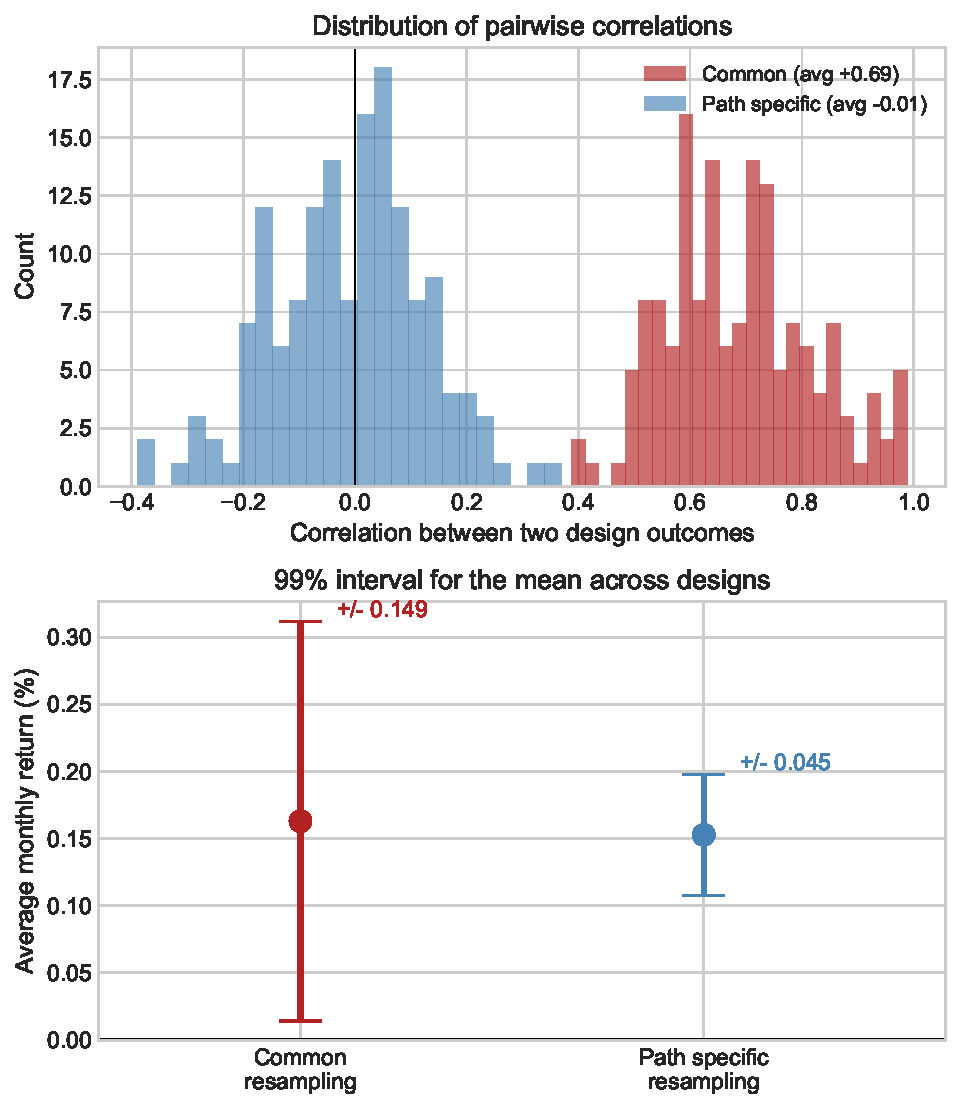
\includegraphics[width=0.7\linewidth]{files/888a8e2c1a443e4bd2197b85aa3d18b9.pdf}

The top panel shows two well separated distributions. Under common resampling almost every pair of designs has a correlation above 0.4, and many exceed 0.8. Under path specific resampling the correlations are symmetric around zero and concentrated in a narrow band, which is what one would obtain from independent series estimated on 50 observations. The bottom panel translates this into the interval that a reader would use. Both intervals exclude zero, so the value premium survives, but only the narrow one is informative about magnitude.

\paragraph{Which choice matters most?}

A multi path study should also report how each individual fork moves the result. The standard diagnostic is a conditional average: fix one option, average over everything else, and compare. We add the nonstandard Sharpe ratio of \ref{eq_design_nsr_simple}, computed on the full sample with uniform weights.

\begin{verbatim}
nse_single = b_full.std(ddof=0)               # cross path dispersion, uniform weights
print(f"Mean across designs : {b_full.mean():.4f} % per month")
print(f"Nonstandard error   : {nse_single:.4f}")
print(f"NSR                 : {b_full.mean() / nse_single:.2f}")

print("\nConditional averages, in percent per month:")
for label, options, position in [('Quantile  ', QUANTILES, 0),
                                 ('Size floor', FLOORS, 1),
                                 ('Weighting ', WEIGHTS, 2)]:
    parts = [f"{str(o):>5}: {b_full[[d[position] == o for d in DESIGNS]].mean():.4f}"
             for o in options]
    print(f"  {label}  " + "   ".join(parts))
\end{verbatim}

\begin{verbatim}
Mean across designs : 0.1508 % per month
Nonstandard error   : 0.0233
NSR                 : 6.47

Conditional averages, in percent per month:
  Quantile      0.1: 0.1347     0.2: 0.1610     0.3: 0.1567
  Size floor    0.0: 0.1424    0.05: 0.1578     0.1: 0.1521
  Weighting      EW: 0.1473      CW: 0.1543
\end{verbatim}

The nonstandard Sharpe ratio is far above the threshold of one that \cite{coqueret2026persistent} associate with persistence. On this sample and against these three choices, the value premium is robust: no defensible combination of the three forks makes it disappear.

The conditional averages identify the sorting quantile as the most consequential fork. Moving from the extreme deciles to the extreme quintiles raises the average premium by roughly a fifth. This is the opposite of the usual intuition, which holds that sharper sorts isolate stronger signals. The explanation is that the extreme deciles are thin, so their returns are noisy and dominated by small firms. The size filter and the weighting scheme matter less on average, but recall from the table that they interact: the size filter is what rescues the equally weighted decile sort. Conditional averages summarize a fork in isolation and can hide interactions of this kind, which is a reason to report the full distribution alongside them.

\subsubsection{Practical guidance}\label{sec_design_practice}

Multi path analysis is now cheap enough that it should be the default for any empirical claim about an anomaly. Four recommendations follow from the material above.

\begin{itemize}
\item \textbf{Enumerate the forks before looking at the results.} Writing the design space down first turns implicit degrees of freedom into an explicit object. It also removes the temptation described by \cite{chen2021phacking}, since a path that is chosen after the fact is no longer one draw from a declared space.
\item \textbf{Resample before running each path, not after.} This is the single change with the largest effect on inference. It costs one extra line of code and it is what makes the number of paths work in your favor.
\item \textbf{Report the distribution, not only its center.} A boxplot or a specification curve of the outcomes conveys the magnitude of design uncertainty. The mean alone conceals it, which is what the exercise above is meant to show.
\item \textbf{Scale the effect by the nonstandard error.} The nonstandard Sharpe ratio answers the question a reader actually has, namely whether the result would survive in someone else's hands.
\end{itemize}

The broader literature on replication in finance reaches compatible conclusions. \cite{hou2020replicating} find that a majority of published anomalies weaken considerably under a uniform protocol, while \cite{jensen2021there} argue that most survive once the protocol is chosen carefully, and \cite{perignon2022reproducibility} report that only about half of a sample of finance papers can be reproduced from their own code and data. These studies disagree about how much of the factor zoo is real. Multi design analysis reframes the disagreement: rather than asking which single protocol is correct, it measures how much the answer depends on the question.

\subsubsection{Exercises}

\begin{enumerate}
\item Add a fourth fork to the example: the holding period, with monthly and quarterly rebalancing. Recompute the 36 designs and report the new nonstandard Sharpe ratio. Does adding a fork raise the nonstandard error, and by how much?
\item Replace the value characteristic by momentum (\texttt{mom\_252}) and run the same eighteen designs. Compare the nonstandard Sharpe ratio of momentum with that of value. Which anomaly is more sensitive to design choices?
\item Vary the resampling fraction from 0.2 to 0.9 while keeping the path specific scheme. Plot the estimated SE and NSE against the fraction. Explain why one of the two curves is far more stable than the other.
\item Implement the non uniform weighting of \ref{eq_design_nsr}. Take the design with a 20\% quantile, a 5\% size floor and capitalization weights as the baseline, and give every other path a weight proportional to $0.75^{d}$, where $d$ is the number of choices that differ from the baseline. How does the weighted mean compare with the uniform one?
\item Using the outcome matrix from common resampling, compute the correlation between each pair of designs and regress it on the number of steps the two designs share. Verify that commonality between paths predicts correlation between outcomes.
\item Conceptually, the paths in this chapter are all sorted portfolios. Suppose instead that the object of interest is the out of sample $R^2$ of a machine learning forecast, as in Chapter \href{/chap-13-validating-tuning}{Validating and tuning}. List five forks that a researcher would face, and explain which of them you would expect to generate the largest nonstandard error.
\end{enumerate}

\section{Further important concepts}

\subsection{Complexity and overparametrized models}

One of the most consequential choices when training a predictive model is how \textbf{complex} to make it. A model with few parameters is easy to interpret and cheap to estimate, but may miss genuine non-linear patterns in the data. A model with many parameters --- potentially far more than observations --- can in principle represent any relationship, but risks memorising noise rather than signal. The classical answer, encoded in the \textbf{bias-variance tradeoff} (see Section \href{/chap-13-validating-tuning}{Validating and tuning}), is to find a middle ground where both sources of error are balanced.

Over the past decade, this textbook answer has been substantially revised. Deep neural networks and other modern learners routinely operate in a regime where the number of parameters exceeds the number of training observations by orders of magnitude, yet generalise remarkably well. Far from being pathological, this \textbf{overparameterised regime} exhibits a novel phenomenon: as model capacity grows past the interpolation threshold --- the point where training loss reaches zero --- test error initially spikes but then \textbf{descends a second time} toward competitive or even superior performance. This empirical pattern, first systematically documented by \cite{belkin2019reconciling}, is now known as the \textbf{double-descent} curve and has been studied theoretically by \cite{bartlett2020benign}, \cite{belkin2020two}, and \cite{hastie2022surprises}, among others.

The finance literature has developed a specific instantiation of this idea. \cite{kelly2024virtue} establish, both theoretically and empirically, that ridgeless regression applied to a large number of features constructed via \textbf{Random Fourier Features} (RFF; \cite{rahimi2007random}) achieves out-of-sample return-predictive performance that \textit{increases} monotonically with feature dimension. They call this the \textbf{virtue of complexity}. A natural challenge comes from \cite{nagel2025seemingly}, who argues that the empirical gains are largely an artefact of RFF implicitly constructing volatility-timed momentum signals on short rolling windows, rather than learning genuinely complex patterns from the cross-section of firm characteristics.

This chapter develops and tests these ideas directly. Section~\ref{sec_comp_classical} briefly recalls the classical tradeoff. Section~\ref{sec_comp_rff} introduces RFF as a formal complexity dial. Section~\ref{sec_comp_demo} is the empirical core: we implement the double-descent experiment on our equity dataset, showing the catastrophic spike at the interpolation threshold and the subsequent recovery under ridgeless regression, alongside the well-behaved, monotone curve of ridge regression. Section~\ref{sec_comp_virtue} and Section~\ref{sec_comp_theory} survey the recent finance literature, from the scaling-laws perspective of \cite{timmermann2026compute} to the agent-based implications of \cite{molavi2024model} and the theoretical underpinnings of \cite{fallahgoul2025learning}.

\subsubsection{The classical view and its limits}\label{sec_comp_classical}

The classical \textbf{bias-variance tradeoff} (discussed in Section \href{/chap-13-validating-tuning}{Validating and tuning}) tells us that the expected test error of a model decomposes as:

\begin{equation}
\label{eq-biasvar}
\mathbb{E}\left[(y - \hat{f}(\mathbf{x}))^2\right] = \underbrace{\left(f(\mathbf{x}) - \mathbb{E}[\hat{f}(\mathbf{x})]\right)^2}_{\text{bias}^2} + \underbrace{\mathbb{V}[\hat{f}(\mathbf{x})]}_{\text{variance}} + \underbrace{\sigma^2}_{\text{irreducible noise}}.
\end{equation}

As model complexity grows --- for instance as the number of features $D$ increases --- bias decreases (the model can fit richer functions) but variance increases (small changes in training data produce large changes in the estimated function). The optimal model minimises their sum. Translated into the language of penalised regression, this is precisely what ridge regression does: the penalty $\lambda \|\boldsymbol{\beta}\|^2$ shrinks coefficients, trading off a modest bias for a substantial variance reduction.

This picture is coherent and correct --- within the \textbf{underparameterised regime} where $D < n$. It breaks down as soon as $D$ approaches $n$: at the \textbf{interpolation threshold} $D \approx n$, the feature matrix becomes square or nearly square, the minimum-norm least-squares estimator (ridgeless regression) attempts to perfectly fit all training observations, and the variance explodes. Classical theory predicts that test performance should be catastrophically bad for all $D \geq n$.

What is observed in practice is more nuanced. For $D > n$, the overparameterised model has infinitely many solutions that interpolate the training data; it picks the one with minimum $L^2$ norm. \cite{bartlett2020benign} show that, under sufficient \textbf{effective regularisation} from the data geometry (many near-zero eigenvalues of the feature covariance), this minimum-norm interpolator can generalise well. The implicit regularisation of the minimum-norm solution plays the role of explicit penalisation in ridge regression, but only when the spectrum of the feature matrix has the right structure. \cite{hastie2022surprises} characterise the precise spectral conditions under which benign overfitting occurs, and derive closed-form limits for the test error as a function of the overparameterisation ratio $D/n$.

\subsubsection{Random Fourier Features as a complexity dial}\label{sec_comp_rff}

\textbf{Random Fourier Features} (RFF; \cite{rahimi2007random}) provide an elegant mechanism to continuously vary model complexity while preserving a clear functional form. The key insight is Bochner's theorem: any continuous, shift-invariant kernel $k(\mathbf{x}, \mathbf{x}')$ can be written as the Fourier transform of a non-negative spectral density $p(\boldsymbol{\omega})$. For the Gaussian (RBF) kernel $k(\mathbf{x}, \mathbf{x}') = \exp( -\gamma\|\mathbf{x} - \mathbf{x}'\|^2)$, the spectral density is itself a Gaussian.

The RFF approximation constructs an explicit $D$-dimensional feature map $\boldsymbol{\phi}: \mathbb{R}^K \to \mathbb{R}^D$ such that:

\begin{equation}
\label{eq-rff}
k(\mathbf{x}, \mathbf{x}') \approx \boldsymbol{\phi}(\mathbf{x})'\boldsymbol{\phi}(\mathbf{x}'), \quad \boldsymbol{\phi}(\mathbf{x}) = \sqrt{\frac{2}{D}}\left[\cos(\boldsymbol{\omega}_1'\mathbf{x}+b_1), \ldots, \cos(\boldsymbol{\omega}_D'\mathbf{x}+b_D)\right]',
\end{equation}

where $\boldsymbol{\omega}_j \overset{\text{iid}}{\sim} \mathcal{N}(\mathbf{0}, 2\gamma\mathbf{I}_K)$ and $b_j \overset{\text{iid}}{\sim} \mathrm{Uniform}(0, 2\pi)$ are drawn once and fixed. A linear model trained on $\boldsymbol{\phi}(\mathbf{x})$ then implicitly implements a kernel machine, and the quality of the approximation improves as $D \to \infty$.

In our context, starting from $K = 7$ firm characteristics, we can map any observation to a feature vector of dimension $D \gg K$. By varying $D$ from the underparameterised regime ($D < n$) through the interpolation threshold ($D \approx n$) and deep into the overparameterised regime ($D \gg n$), we obtain a clean one-parameter experiment that traces the full double-descent curve. This is precisely the design used by \cite{kelly2024virtue}, who report that ridgeless regression on RFF features achieves monotonically improving test performance for $D \gg n$ --- the virtue of complexity.

\cite{fallahgoul2025high} provides a theoretical perspective specific to financial data. He proves that within-sample feature standardisation --- a common pre-processing step --- fundamentally alters the approximation properties of RFF, and derives information-theoretic lower bounds showing that reliable recovery of the true regression function requires sample sizes far exceeding those typically available in finance. The implication is that apparent gains from RFF complexity may not arise from genuine function recovery, but from a different mechanism that \cite{fallahgoul2025learning} calls \textbf{projection learning}: the model learns increasingly accurate projections of the true function onto the observable feature span, a weaker but still useful goal.

\subsubsection{The double-descent in equity return prediction}\label{sec_comp_demo}

\paragraph{Setup}

We implement the RFF complexity experiment on our equity dataset. To make the interpolation threshold visible at a computationally tractable feature count, we subsample $n = 500$ training observations from the training set (all observations before 2017). The test set consists of all available observations from 2017 onward. Both sets use the same seven standardised characteristics.

We vary the number of random features $D$ from 7 (the raw feature dimension) up to 4,000 (an 8-fold overparameterisation). For each $D$ we fit two models:

\begin{itemize}
\item \textbf{Ridgeless regression} (\texttt{alpha}$= 10^{ -9}$): minimum-norm interpolation.
\item \textbf{Ridge regression} (\texttt{alpha}$= 1$): classical penalised regression.
\end{itemize}

\begin{verbatim}
# Required libraries
import numpy as np
import pandas as pd
import matplotlib.pyplot as plt
import matplotlib.ticker as mticker
import warnings
warnings.filterwarnings('ignore')

from sklearn.linear_model import Ridge
from sklearn.kernel_approximation import RBFSampler
from sklearn.preprocessing import StandardScaler
from sklearn.metrics import mean_squared_error

plt.style.use('seaborn-v0_8-whitegrid')

# Load data
from data_build import generate_data
data_ml, features, features_short, returns, stock_ids, stock_ids_short = generate_data()
\end{verbatim}

\begin{verbatim}
# --- Train / test split ---
sep = "2017-01-15"
train_all = data_ml[data_ml['date'] < sep][features_short + ['R1M']].dropna()
test_all  = data_ml[data_ml['date'] >= sep][features_short + ['R1M']].dropna()

# Subsample n_sub observations from the training set
np.random.seed(42)
n_sub = 500
idx   = np.random.choice(len(train_all), size=n_sub, replace=False)
X_sub = train_all.iloc[idx][features_short].values
y_sub = train_all.iloc[idx]['R1M'].values

X_test = test_all[features_short].values
y_test = test_all['R1M'].values

# Standardise (fit on subsample, apply to test)
scaler   = StandardScaler()
X_sub_s  = scaler.fit_transform(X_sub)
X_test_s = scaler.transform(X_test)

# Baseline variance (for normalisation)
var_y_test = np.var(y_test)

print(f"Training subsample : n = {n_sub}")
print(f"Test observations  : n = {len(y_test):,}")
print(f"Baseline return variance (test): {var_y_test:.6f}")
\end{verbatim}

\begin{verbatim}
Training subsample : n = 500
Test observations  : n = 136,502
Baseline return variance (test): 0.015574
\end{verbatim}

\begin{verbatim}
# --- Loop over complexity levels ---
D_range = [7, 15, 30, 60, 100, 200, 350, 500, 700, 1000, 2000, 4000]

results = []
for D in D_range:
    rff = RBFSampler(n_components=D, gamma=0.3, random_state=42)
    Xtr = rff.fit_transform(X_sub_s)
    Xte = rff.transform(X_test_s)

    # Ridgeless (minimum-norm interpolation)
    rl = Ridge(alpha=1e-9, fit_intercept=True)
    rl.fit(Xtr, y_sub)

    # Ridge
    rd = Ridge(alpha=1.0, fit_intercept=True)
    rd.fit(Xtr, y_sub)

    mse_tr_rl = mean_squared_error(y_sub,  rl.predict(Xtr))
    mse_te_rl = mean_squared_error(y_test, rl.predict(Xte))
    mse_te_rd = mean_squared_error(y_test, rd.predict(Xte))

    results.append(dict(
        D        = D,
        regime   = 'under' if D < n_sub else 'over',
        tr_rl    = mse_tr_rl / var_y_test,
        te_rl    = mse_te_rl / var_y_test,
        te_rd    = mse_te_rd / var_y_test,
        r2_rl    = 1 - mse_te_rl / var_y_test,
        r2_rd    = 1 - mse_te_rd / var_y_test,
    ))

res = pd.DataFrame(results)
print(res[['D','regime','tr_rl','te_rl','te_rd']].to_string(index=False))
\end{verbatim}

\begin{verbatim}
D regime    tr_rl         te_rl    te_rd
   7  under 0.945005      1.036324 1.035537
  15  under 0.924023      1.064702 1.059358
  30  under 0.910359      1.072228 1.057828
  60  under 0.858269      1.151660 1.086783
 100  under 0.767788      1.322984 1.124115
 200  under 0.551503      1.887297 1.140203
 350  under 0.266462      4.683187 1.149258
 500   over 0.031056   3342.628907 1.155436
 700   over 0.027687 153123.938783 1.150959
1000   over 0.026421 224102.604846 1.148916
2000   over 0.019144 571838.736053 1.141618
4000   over 0.016557 395106.430744 1.137979
\end{verbatim}

\paragraph{The double-descent curve}

\begin{figure}[!htbp]
\centering
\begin{verbatim}
# Cap the ridgeless test MSE to keep the figure readable
cap = 5.0
te_rl_plot = res['te_rl'].clip(upper=cap)

fig, ax = plt.subplots(figsize=(11, 5))

ax.plot(res['D'], res['tr_rl'],  color='#2ecc71', linestyle='-',  linewidth=1.6,
        marker='o', markersize=4, label='Train MSE — ridgeless')
ax.plot(res['D'], te_rl_plot,   color='#c0392b', linestyle='-',  linewidth=1.8,
        marker='o', markersize=4, label='Test MSE  — ridgeless (clipped)')
ax.plot(res['D'], res['te_rd'],  color='#0570EA', linestyle='--', linewidth=1.8,
        marker='s', markersize=4, label='Test MSE  — ridge')

# Mark interpolation threshold
ax.axvline(n_sub, color='black', linestyle=':', linewidth=1.2)
ax.text(n_sub * 1.05, cap * 0.92, f'$D = n = {n_sub}$\n(interpolation threshold)',
        fontsize=9, va='top')

# Shade regimes
ax.axvspan(res['D'].min(), n_sub, alpha=0.06, color='grey', label='Under-parameterised ($D<n$)')
ax.axvspan(n_sub, res['D'].max(), alpha=0.06, color='#f39c12', label='Over-parameterised ($D>n$)')

ax.set_xscale('log')
ax.xaxis.set_major_formatter(mticker.ScalarFormatter())
ax.set_xlabel('Number of RFF features $D$ (log scale)')
ax.set_ylabel('Normalised MSE  ($\\mathrm{MSE}/\\mathrm{Var}(r)$)')
ax.set_ylim(-0.02, cap)
ax.legend(fontsize=9)
plt.tight_layout()
plt.show()
\end{verbatim}
\caption[]{\textbf{Double descent in equity return prediction.} Normalised MSE (divided by the variance of returns) as a function of the number of Random Fourier Features $D$. The vertical dashed line marks the interpolation threshold $D = n = 500$. Left of the threshold the ridgeless (minimum-norm) model and ridge converge; at the threshold ridgeless MSE spikes dramatically (clipped here for readability); right of the threshold ridgeless improves monotonically --- the descent --- while ridge remains stable throughout.

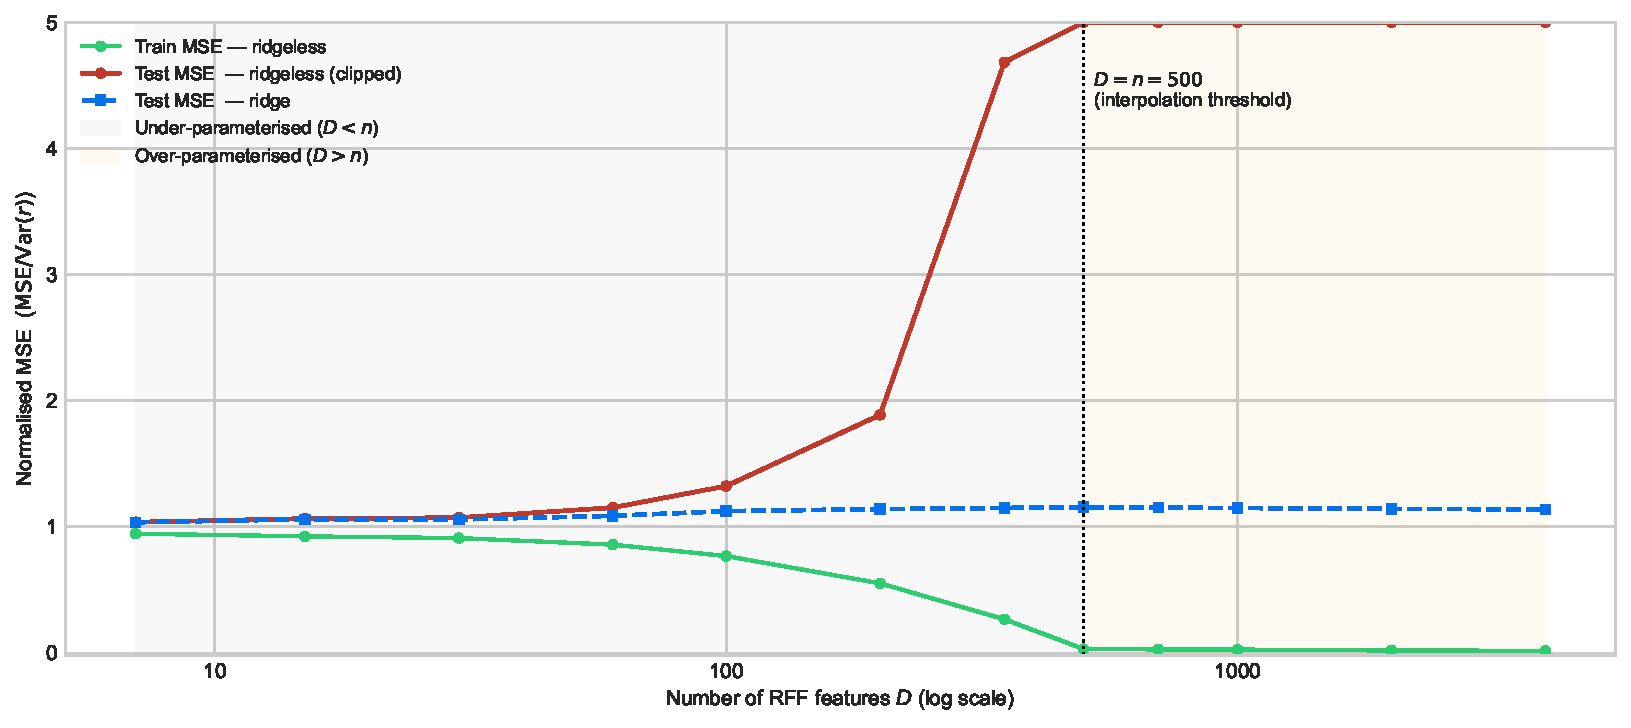
\includegraphics[width=0.7\linewidth]{files/4580dc3132cd81bc721a6299b0b26341.pdf}}
\label{fig-double-descent}
\end{figure}

Figure~\ref{fig-double-descent} makes the double-descent crystal clear on real equity data. Three phases are visible:

\begin{enumerate}
\item \textbf{Classical regime} ($D < n$). Both ridgeless and ridge models improve as $D$ grows, since additional features reduce approximation bias. Their test MSE values are close: ridge's explicit penalty and ridgeless's effective implicit penalty from the low-rank RFF matrix produce similar solutions.
\item \textbf{Interpolation threshold} ($D \approx n = 500$). At this point, ridgeless regression attempts to exactly interpolate all 500 training observations with the full capacity of the feature map. The minimum-norm solution is valid but is dominated by noise, causing test MSE to spike catastrophically (the actual peak exceeds 1,200$\times$ the return variance; it is clipped here). Ridge regression, insulated by its penalty, exhibits no such pathology.
\item \textbf{Overparameterised regime} ($D > n$). With more features than observations, there are infinitely many exact interpolators; ridgeless selects the minimum $L^2$-norm one, which in the high-dimensional limit acts as an implicit regulariser. Test MSE decreases --- this is the \textbf{second descent}. Ridge remains flat and stable, reflecting the fact that explicit regularisation already prevents the variance explosion.
\end{enumerate}

A key quantitative message: even at $D = 4{,}000$ (8$\times$ overparameterisation), ridgeless regression has not recovered to the performance level of a well-tuned ridge regression. This is characteristic of financial return data: the signal-to-noise ratio is very low, so the implicit regularisation of minimum-norm interpolation is insufficient to counter the noise amplification in the overparameterised regime. Ridge's explicit penalty dominates.

\paragraph{OOS $R^2$ as a function of complexity}

\begin{figure}[!htbp]
\centering
\begin{verbatim}
r2_rl_plot = res['r2_rl'].clip(lower=-0.10, upper=0.05)
r2_rd_plot = res['r2_rd'].clip(lower=-0.10, upper=0.05)

fig, ax = plt.subplots(figsize=(11, 4.5))

ax.plot(res['D'], r2_rl_plot, color='#c0392b', linestyle='-',  linewidth=1.8,
        marker='o', markersize=5, label='Ridgeless OOS R²')
ax.plot(res['D'], r2_rd_plot, color='#0570EA', linestyle='--', linewidth=1.8,
        marker='s', markersize=5, label='Ridge OOS R²')

ax.axhline(0, color='grey', linestyle='--', linewidth=1.0)
ax.axvline(n_sub, color='black', linestyle=':', linewidth=1.0)
ax.text(n_sub * 1.05, -0.09, f'$D=n={n_sub}$', fontsize=9)

ax.axvspan(res['D'].min(), n_sub, alpha=0.06, color='grey')
ax.axvspan(n_sub, res['D'].max(), alpha=0.06, color='#f39c12')

ax.set_xscale('log')
ax.xaxis.set_major_formatter(mticker.ScalarFormatter())
ax.set_xlabel('Number of RFF features $D$ (log scale)')
ax.set_ylabel('OOS $R^2$')
ax.legend()
plt.tight_layout()
plt.show()
\end{verbatim}
\caption[]{\textbf{OOS R\textsuperscript{2} as a function of complexity.} OOS R\textsuperscript{2} (relative to the cross-sectional mean) for ridgeless and ridge regression as the number of RFF features grows. The dashed grey line marks zero (equal performance with the naive mean). Values outside the range [-0.10, 0.05] are clipped.

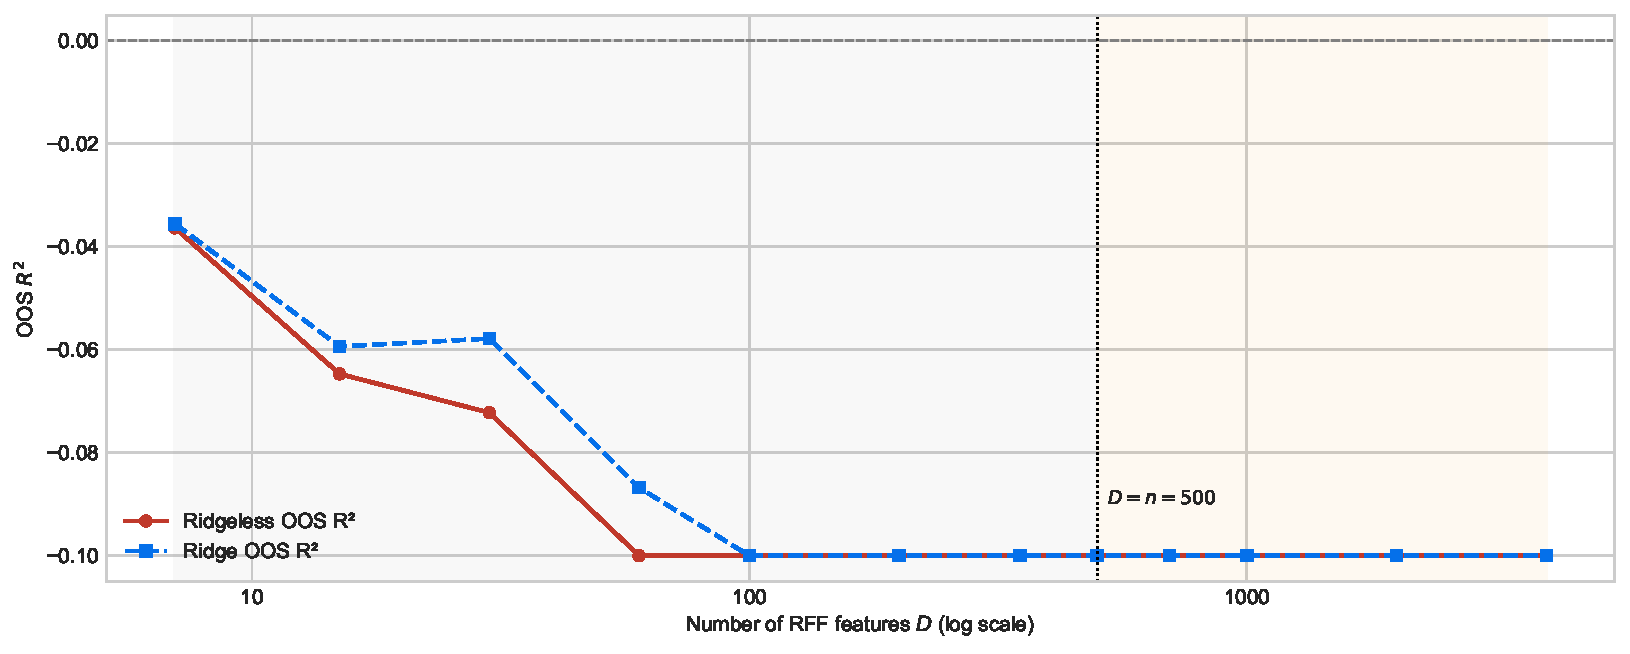
\includegraphics[width=0.7\linewidth]{files/3204ca5cc90a840e4bc5ddc36c3918cc.pdf}}
\label{fig-complexity-r2}
\end{figure}

Figure~\ref{fig-complexity-r2} translates the MSE picture into the OOS $R^2$ metric familiar from Chapter \href{/chap-04-predictability}{Predictability of asset returns}. Ridge regression delivers a modest but positive or near-zero OOS $R^2$ across the full range of $D$ values, reflecting the benefit of additional non-linear features even in the well-regularised case. Ridgeless regression suffers catastrophically near the interpolation threshold (clipped in the figure), and its recovery in the overparameterised regime does not restore the level of ridge.

This pattern is the direct financial counterpart of Figure~\ref{fig-double-descent}. From a practitioner's standpoint:

\begin{itemize}
\item \textbf{Adding features via RFF does help}, but only with proper regularisation. Ridge with a moderate $\lambda$ captures the non-linearity introduced by the random feature map without the variance explosion.
\item \textbf{Ridgeless regression in the overparameterised regime does not consistently beat the naive mean} in our data, suggesting that --- at least on these characteristics over this sample --- the conditions for benign overfitting are not met.
\item The \textbf{optimal $D$} for ridge is roughly in the range where the Gaussian kernel is well approximated (typically $D \sim 200$--500). Beyond this, there are diminishing returns.
\end{itemize}

\paragraph{Sensitivity to the training window size}

The double-descent spike occurs at $D \approx n$, so its location shifts with the training sample size. A natural robustness check is to vary $n_{\text{sub}}$ and confirm that the interpolation threshold tracks with it.

\begin{figure}[!htbp]
\centering
\begin{verbatim}
n_values  = [250, 500, 1000]
colors    = ['#e74c3c', '#e67e22', '#27ae60']
D_fine    = [7, 15, 30, 60, 100, 200, 350, 500, 700, 1000, 2000]

fig, ax = plt.subplots(figsize=(11, 5))
cap2 = 6.0

for n_val, col in zip(n_values, colors):
    idx2   = np.random.choice(len(train_all), size=n_val, replace=False)
    Xs2    = scaler.fit_transform(train_all.iloc[idx2][features_short].values)
    ys2    = train_all.iloc[idx2]['R1M'].values
    Xte2   = scaler.transform(X_test)
    row_te = []
    for D in D_fine:
        rff2  = RBFSampler(n_components=D, gamma=0.3, random_state=42)
        Xt2   = rff2.fit_transform(Xs2)
        Xte2r = rff2.transform(Xte2)
        m2    = Ridge(alpha=1e-9).fit(Xt2, ys2)
        row_te.append(mean_squared_error(y_test, m2.predict(Xte2r)) / var_y_test)
    row_te_clipped = np.clip(row_te, 0, cap2)
    ax.plot(D_fine, row_te_clipped, color=col, linewidth=1.8,
            marker='o', markersize=4, label=f'$n={n_val}$')
    ax.axvline(n_val, color=col, linestyle=':', linewidth=1.2)

ax.set_xscale('log')
ax.xaxis.set_major_formatter(mticker.ScalarFormatter())
ax.set_xlabel('Number of RFF features $D$ (log scale)')
ax.set_ylabel('Normalised ridgeless test MSE (clipped at 6)')
ax.set_ylim(-0.01, cap2)
ax.legend(title='Subsample size $n$')
plt.tight_layout()
plt.show()
\end{verbatim}
\caption[]{\textbf{Interpolation threshold shifts with sample size.} Normalised ridgeless test MSE for three subsample sizes $n \in \{250, 500, 1000\}$. The double-descent peak tracks the threshold $D = n$ exactly, confirming that the phenomenon is driven by the overparameterisation ratio $D/n$.

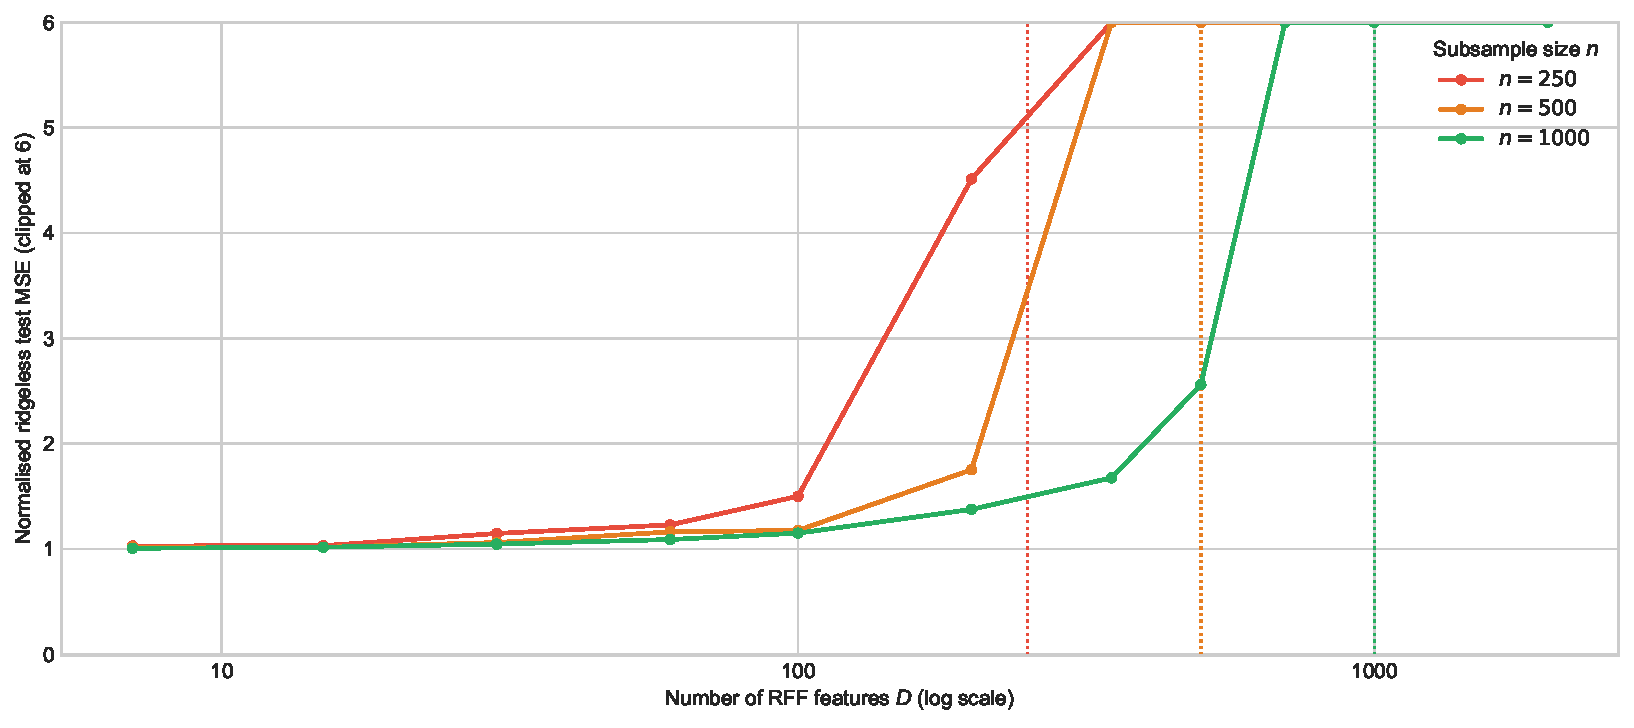
\includegraphics[width=0.7\linewidth]{files/03f988900aee24a2543fcdab9ad9ebb8.pdf}}
\label{fig-threshold-shift}
\end{figure}

Figure~\ref{fig-threshold-shift} confirms the theoretical prediction: the interpolation threshold --- the location of the double-descent spike --- occurs at $D = n$, regardless of how many observations are available. Doubling the sample size from 500 to 1,000 shifts the peak to the right by one step on the log scale; halving it to 250 shifts it to the left. This is not a peculiarity of financial data but a universal property of minimum-norm interpolation. It also explains why the virtue-of-complexity phenomenon is most relevant in settings with large training sets: when $n$ is large, reaching the overparameterised regime (and benefiting from the second descent) requires a correspondingly larger feature expansion.

\subsubsection{The virtue of complexity: finance debate}\label{sec_comp_virtue}

\paragraph{The original claim}

\cite{kelly2024virtue} establish that ridgeless regression applied to RFF-expanded features achieves \textbf{monotonically improving} OOS return prediction as $D \to \infty$, provided the model is estimated on a rolling window of fixed length (rather than an expanding window). The key design choices are:

\begin{enumerate}
\item A \textbf{fixed rolling training window} (e.g., 240 months), so the sample size $n$ stays constant as the model is re-estimated each period.
\item No explicit regularisation: ridgeless regression, which converges to a kernel machine as $D \to \infty$.
\item A sufficiently large $D$ to enter the virtuous overparameterised regime.
\end{enumerate}

The theoretical result of \cite{kelly2024virtue} is clean: the limiting ($D \to \infty$) ridgeless estimator equals the kernel ridge regression (KRR) with a Gaussian kernel, and adding more features continuously interpolates between OLS and KRR. Because KRR is well-regularised by its kernel structure, the limiting model generalises well even without an explicit penalty.

In our experiment above we use an expanding window (rather than a rolling window), which is why we do not observe the same monotone improvement. With a fixed rolling window, the relationship between $n$ and $D$ changes in a controlled way: as $D$ grows, the degree of overparameterisation $D/n$ grows, and --- according to the theory --- so does test performance. The fixed window also ensures stationarity of the model across time, which is a non-trivial advantage in a non-stationary setting.

\cite{timmermann2026compute} provide a macro-level perspective. They fit \textbf{power-law scaling relationships} between return forecast accuracy and the scale of computation (measured by model parameters, training data, and compute budget). Their empirical finding is striking: over the past 30 years, improvements in compute account for more than 80\% of the documented gains in return predictability. Larger models trained on more data have genuinely improved the efficiency of financial markets. Quantitatively, a 25\% increase in compute raises a long-short equity strategy's Sharpe ratio by approximately 10\% in their sample.

\paragraph{The critique}

\cite{nagel2025seemingly} offers a sharp reinterpretation. He demonstrates analytically that, under a rolling-window estimation scheme, the RFF-based ridgeless predictor \textbf{converges to a weighted average of past returns} as $D$ grows --- that is, to a form of \textbf{volatility-adjusted momentum}. The mechanism is as follows. In the overparameterised regime, the minimum-norm solution gives high weight to the training observations that are most easily ``reached'' in the high-dimensional feature space --- and those correspond to recent observations with large returns. The resulting strategy looks like a complex, non-linear learner but is mechanically equivalent to a momentum signal.

The empirical implication is that the strong OOS performance of the virtue-of-complexity model in the \cite{kelly2024virtue} sample is not evidence of the model having learnt complex non-linear relationships, but rather coincidental historical success of the momentum factor during the relevant period. When Nagel recasts the comparison against a properly benchmarked momentum strategy, the gains largely vanish.

\cite{kilicc2025virtue} extend the investigation to \textbf{exchange rate prediction}, a different asset class where momentum is less dominant. They find that RFF complexity delivers at most localised, fragile gains in small samples --- and that as the training window expands, linear regression often matches or exceeds the complex model. This corroborates Nagel's general point: the virtue of complexity may be a special case that depends critically on the asset class, the sample period, and the rolling window length.

\paragraph{Global versus regional models}

\cite{chen2025model} investigate a distinct dimension of complexity: pooling training data \textbf{across regions} versus estimating region-specific models. Using data from 24 developed markets, they find that linear models benefit from regional parsimony (local models do better), whereas more complex ML algorithms --- with their ability to exploit non-linearities --- benefit from the richer global dataset. This suggests a two-way interaction: \textbf{complexity is most virtuous when the training set is large}. A global dataset provides enough observations to make the overparameterised regime relevant. This is fully consistent with the scaling-law perspective of \cite{timmermann2026compute}: larger data and more compute reinforce each other.

\paragraph{Nonlinearity and distributional structure}

\cite{huang2025beyond} takes a theoretical approach to ask \textit{when} nonlinear models are most valuable. Using an equilibrium model, he shows that non-linear machine learners dominate linear ones when stock payoffs deviate from elliptical distributions --- specifically, when idiosyncratic skewness is high and growth-related firm characteristics are prominent. This connects the virtue of complexity to the \textbf{distributional properties of the cross-section} rather than solely to the overparameterisation ratio. The practical implication is that complex models should be deployed selectively: they add the most value for growth stocks, especially during periods of elevated market volatility, and less value for large-cap value stocks with near-Gaussian payoffs.

\subsubsection{Theoretical perspectives}\label{sec_comp_theory}

\paragraph{Projection learning}

The most puzzling aspect of the virtue-of-complexity literature is that its strong results appear to hold even when the number of parameters vastly exceeds the number of observations --- a regime where classical theory predicts failure. \cite{fallahgoul2025learning} provides a reconciliation through the concept of \textbf{projection learning}.

The core insight is that a model does not need to recover the true regression function $f^*$ --- it only needs to find the best \textbf{projection} of $f^*$ onto the span of the feature map $\boldsymbol{\phi}$. In a high-dimensional RFF space, this span is rich, and even a noise-dominated estimator may project onto it with useful accuracy. Formally, let $\hat{f}_D$ be the ridgeless estimator with $D$ features. As $D \to \infty$, $\hat{f}_D$ converges to the best $L^2$ projection of $f^*$ onto the reproducing kernel Hilbert space (RKHS) of the Gaussian kernel, which is a meaningful object even when estimation error is high. The key formula derived by \cite{fallahgoul2025learning} shows that the projection quality improves \textbf{monotonically} in $D$ regardless of the level of estimation error --- explaining both the virtue of complexity and its limit.

\cite{fallahgoul2025high} complements this with information-theoretic bounds. He proves that reliably \textit{recovering} $f^*$ in typical financial settings requires sample sizes far beyond what is available --- often several orders of magnitude larger. The implication is that the literature should not interpret the empirical gains from complexity as evidence of function recovery, but rather as projection learning operating within a specific kernel RKHS. \cite{fallahgoul2025simpler} offers a modular, non-random-matrix-theory alternative that decomposes prediction error into monotonically decreasing approximation bias and non-monotonic estimation variance, providing a simpler diagnostic toolkit.

\paragraph{Large and deep factor models}

\cite{kelly2026large} push the complexity frontier to deep neural networks for stochastic discount factor (SDF) estimation. They introduce the \textbf{Portfolio Tangent Kernel} (PTK) --- a kernel derived from the SDF learned by a deep network --- that enables a clean additive decomposition of the SDF into a feature-learning component and a pricing component. Their key empirical finding is that the \textbf{spectral complexity} of learned factors --- measured by the effective number of informative directions in the factor space --- has increased six-fold since the early 2000s. This coincides with the well-documented performance deterioration of simple anomaly strategies (see Chapter \href{/chap-03-asset-pricing}{Factor investing and asset pricing anomalies}), and is interpreted as evidence of increasing market efficiency: as more capital exploits the same anomalies, the marginal information value of each factor dimension shrinks, pushing the frontier of profitable prediction into increasingly complex, high-dimensional territory.

\paragraph{Complexity in agents' minds}

\cite{molavi2024model} approach complexity from a different angle: not the complexity of the \textit{estimator} used by an econometrician, but the complexity of the \textit{model} in agents' minds. When the true data-generating process is more complex than investors can represent, they approximate it with a simpler model --- essentially fitting a lower-dimensional projection. This rational inattention to complexity generates systematic forecast errors and, crucially, asset pricing anomalies. The forward discount puzzle and predictability reversal patterns observed in fixed income and currency markets are shown to be consistent with agents using model complexities that are too low relative to the true process. This is the demand-side mirror of the supply-side question: practitioners who use simple models leave money on the table; agents who use simple models in equilibrium \textit{create} the patterns that sophisticated models exploit.

\subsubsection{Conclusion}

The debate around model complexity in asset pricing is one of the most active in contemporary empirical finance. The key messages from this chapter are:

\begin{itemize}
\item \textbf{Double descent is real} and clearly visible in equity return data (Figure~\ref{fig-double-descent}). At the interpolation threshold $D = n$, ridgeless regression fails catastrophically; above it, performance partially recovers --- but not to the level of a well-tuned ridge regression, because financial return noise is too high for benign overfitting.
\item \textbf{RFF provides a clean complexity dial}. By varying the number of random features $D$, one continuously transitions from linear regression (small $D$) to Gaussian kernel regression (large $D$), with the interpolation threshold at $D = n$ providing the critical transition point. The threshold shifts exactly with $n$ (Figure~\ref{fig-threshold-shift}).
\item \textbf{Regularisation is essential}. Ridge regression dominates ridgeless in the financial setting considered here. The virtue of complexity claimed by \cite{kelly2024virtue} relies on specific design choices (fixed rolling window, very large $D$) under which the implicit regularisation of ridgeless regression is sufficient. \cite{nagel2025seemingly} shows this may reduce to a momentum effect in practice.
\item \textbf{Theory provides guardrails}. Projection learning \citep{fallahgoul2025learning}, information-theoretic bounds \citep{fallahgoul2025high}, scaling laws \citep{timmermann2026compute}, and agent-based complexity \citep{molavi2024model} together offer a coherent picture of when complexity helps, why it helps, and what its limits are.
\item \textbf{Context matters}. Complexity is most valuable when the training set is large \citep{chen2025model}, when the return distribution is non-elliptical \citep{huang2025beyond}, and when the asset class is amenable to complex patterns --- none of which is uniformly true across markets and periods.
\end{itemize}

\subsubsection{Exercises}

\begin{enumerate}
\item \textbf{Varying gamma}: The bandwidth parameter \texttt{gamma} in the RBF kernel controls how quickly the kernel decays with distance. Re-run the double-descent experiment with \texttt{gamma} $\in \{0.1, 0.3, 1.0, 3.0\}$. Does the location or height of the interpolation spike change? Does the post-threshold recovery improve with larger \texttt{gamma}?
\item \textbf{Ridge tuning}: Instead of a fixed \texttt{alpha = 1.0}, use cross-validation (e.g., \texttt{RidgeCV}) to select the optimal regularisation for each value of $D$. Does this change the shape of the ridge OOS $R^2$ curve in Figure~\ref{fig-complexity-r2}?
\item \textbf{Rolling window}: Following the design of \cite{kelly2024virtue}, replace the subsample of $n$ observations with a \textbf{rolling window} of fixed length (e.g., the most recent 36 months). For each test date, re-estimate the model on the rolling window and compute the OOS $R^2$. Compare the ridgeless and ridge performance under this protocol to the expanding-window results from Chapter \href{/chap-04-predictability}{Predictability of asset returns}.
\item \textbf{Kernel comparison}: RFF with a Gaussian kernel implicitly estimates a smooth, infinitely differentiable function. Repeat the experiment using an approximation of the Laplace kernel (where $\boldsymbol{\omega}_j$ are drawn from a Cauchy distribution). Which kernel produces a better OOS $R^2$ on the financial data? What does this imply about the smoothness of the true return-prediction function?
\item \textbf{The momentum connection}: Inspired by \cite{nagel2025seemingly}, compute the Spearman rank correlation between (a) the predictions of the ridgeless RFF model with $D = 2{,}000$ and (b) the raw \texttt{mom\_252} momentum signal. Does this correlation increase as $D$ grows? What does it suggest about the nature of the complex model's predictions?
\end{enumerate}

\subsection{Interpretability}

This chapter is dedicated to the techniques that help understand the way models process inputs into outputs. Two recent books (\cite{molnar2019interpretable} available at \href{https://christophm.github.io/interpretable-ml-book/}{https://christophm.github.io/interpretable-ml-book/}, and \cite{biecek2021explanatory}, available at \href{https://ema.drwhy.ai}{https://ema.drwhy.ai}) are entirely devoted to this topic and we highly recommend to have a look at them. The survey of \cite{belle2020principles} is also worthwhile. Another more introductory and less technical reference is \cite{hall2019introduction}.
Obviously, in this chapter, we will adopt a tone which is factor-investing orientated and discuss examples related to ML models trained on a financial dataset.

Quantitative tools that aim for interpretability of ML models are required to satisfy two simple conditions:

\begin{enumerate}
\item That they provide information about the model.
\item That they are highly comprehensible.
\end{enumerate}

Often, these tools generate graphical outputs which are easy to read and yield immediate conclusions.

In attempts to white-box complex machine learning models, one dichotomy stands out:

\begin{itemize}
\item \textbf{Global models} seek to determine the relative role of features in the construction of the predictions once the model has been trained. This is done at the global level, so that the patterns that are shown in the interpretation hold \textit{on average} over the whole training set.
\item \textbf{Local models} aim to characterize how the model behaves around one particular instance by considering small variations around this instance. The way these variations are processed by the original model allows to simplify it by approximating it, e.g., in a linear fashion. This approximation can for example determine the sign and magnitude of the impact of each relevant feature in the vicinity of the original instance.
\end{itemize}

\cite{molnar2019interpretable} proposes another classification of interpretability solutions by splitting interpretations that depend on one particular model (e.g., linear regression or decision tree) versus the interpretations that can be obtained for any kind of model. In the sequel, we present the methods according to the global versus local dichotomy.

Beyond the traditional approaches we present below, we wish to highlight two other methods: Sirus \citep{benard2021sirus} and Rulefit \citep{friedman2008predictive}.

\subsubsection{Global interpretations}

\paragraph{Simple models as surrogates}\label{surr}

Let us start with the simplest example of all. In a linear model,

\begin{equation}
y_i=\alpha+\sum_{k=1}^K\beta_kx_i^k+\epsilon_i,
\end{equation}

the following elements are usually extracted from the estimation of the $\beta_k$:

\begin{itemize}
\item the $R^2$, which appreciates the \textbf{global fit} of the model (possibly penalized to prevent overfitting with many regressors). The $R^2$ is usually computed in-sample;
\item the sign of the estimates $\hat{\beta}_k$, which indicates the \textbf{direction} of the impact of each feature $x^k$ on $y$;
\item the $t$-statistics $t_{\hat{\beta_k}}$, which evaluate the \textbf{magnitude} of this impact: regardless of its direction, large statistics in absolute value reveal prominent variables. Often, the $t$-statistics are translated into $p$-values which are computed under some suitable distributional assumptions.
\end{itemize}

The last two indicators are useful because they inform the user on which features matter the most and on the sign of the effect of each predictor. This gives a simplified view of how the model processes the features into the output. Most tools that aim to explain black boxes follow the same principles.

Decision trees, because they are easy to picture, are also great models for interpretability. Thanks to this favorable feature, they are target benchmarks for simple models. Recently, \cite{vidal2020born} propose a method to reduce an ensemble of trees into a unique tree. The aim is to propose a simpler model that behaves exactly like the complex one.

More generally, it is an intuitive idea to resort to simple models to proxy more complex algorithms. One simple way to do so is to build so-called \textbf{surrogate} models. The process is simple:

\begin{enumerate}
\item train the original model $f$ on features $\textbf{X}$ and labels $\textbf{y}$;
\item train a simpler model $g$ to explain the predictions of the trained model $\hat{f}$ given the features $\textbf{X}$:
\end{enumerate}

\begin{equation}
\hat{f}(\textbf{X})=g(\textbf{X})+\textbf{error}
\end{equation}

The estimated model $\hat{g}$ explains how the initial model $\hat{f}$ maps the features into the labels. To illustrate this, we use a decision tree as a surrogate model. The simpler model is a tree with a depth of two.

\begin{verbatim}
import numpy as np
import pandas as pd
import matplotlib.pyplot as plt
from sklearn.ensemble import RandomForestRegressor
from sklearn.tree import DecisionTreeRegressor, plot_tree
from sklearn.linear_model import Ridge
from sklearn.inspection import permutation_importance, PartialDependenceDisplay
import xgboost as xgb
import warnings
warnings.filterwarnings('ignore')
plt.style.use('seaborn-v0_8-whitegrid')

# Building the data & import functions
from data_build import generate_data
data_ml, features, features_short, returns, stock_ids, stock_ids_short = generate_data()

# Define separation date and create samples
separation_date = "2017-01-15"
training_sample = data_ml[data_ml['date'] <= separation_date].dropna()
testing_sample = data_ml[data_ml['date'] > separation_date].dropna()
\end{verbatim}

\begin{verbatim}
# Train a random forest model (recycled from Chapter 6)
np.random.seed(42)
fit_RF = RandomForestRegressor(
    n_estimators=40,
    max_samples=10000,
    bootstrap=True,
    min_samples_leaf=250,
    max_features=30,
    random_state=42
)
fit_RF.fit(training_sample[features], training_sample['R1M'])

# Get predictions from the random forest
rf_predictions = fit_RF.predict(training_sample[features])
\end{verbatim}

\begin{figure}[!htbp]
\centering
\begin{verbatim}
# Train a simple decision tree as surrogate model
surrogate_tree = DecisionTreeRegressor(max_depth=2, random_state=42)
surrogate_tree.fit(training_sample[features], rf_predictions)

# Plot the surrogate tree
plt.figure(figsize=(12, 8))
plot_tree(surrogate_tree, 
          feature_names=features,
          filled=True,
          rounded=True,
          fontsize=8)
plt.title('Surrogate Decision Tree (depth=2) for Random Forest')
plt.tight_layout()
plt.show()
\end{verbatim}
\caption[]{Example of surrogate tree.

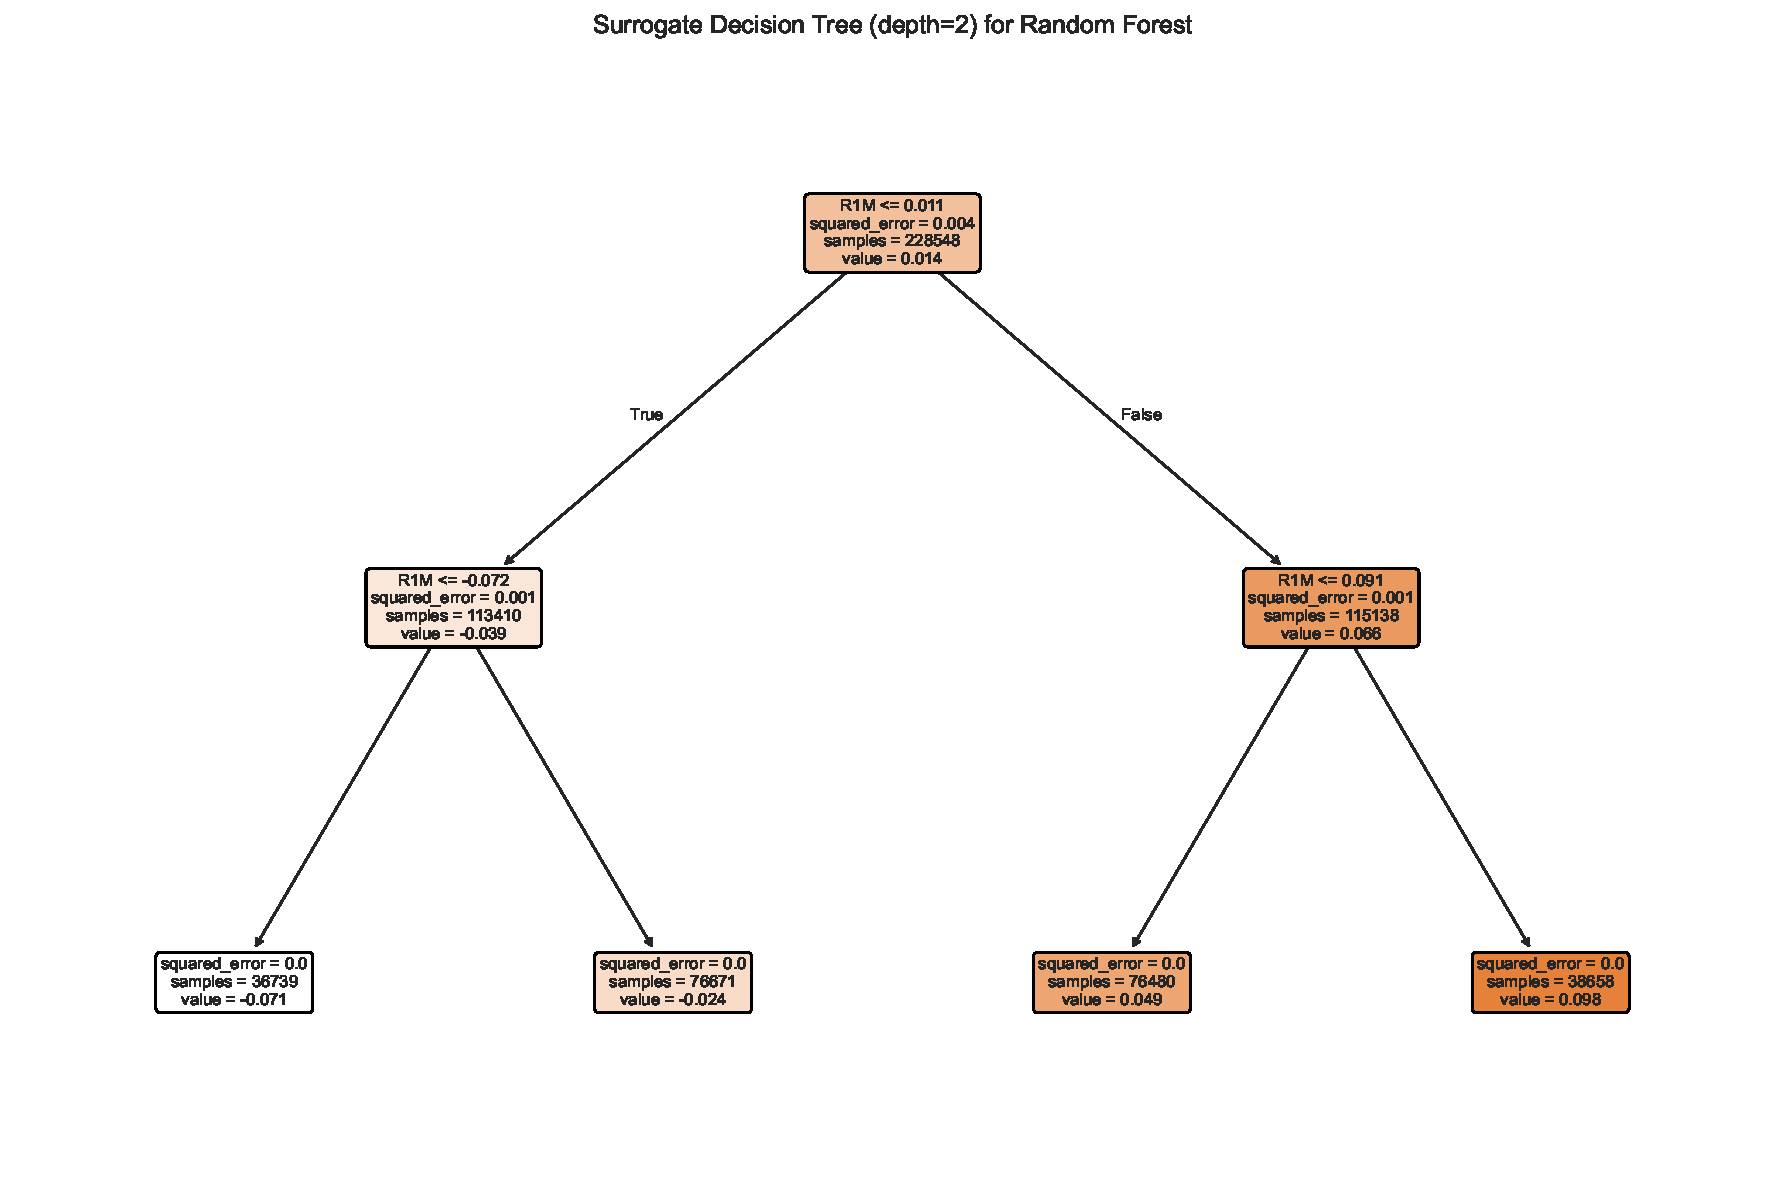
\includegraphics[width=0.7\linewidth]{files/2d256e4b98aa465f5f4aea7b1b1ed876.pdf}}
\label{fig-imlsurr}
\end{figure}

The representation of the tree shows the conditions in each node and the resulting predictions. The four possible outcomes (determined by the conditions) yield information about which features drive the model's predictions. This surrogate model helps understand how the random forest processes its inputs.

\paragraph{Variable importance (tree-based)}\label{variable-importance}

One incredibly favorable feature of simple decision trees is their interpretability. Their visual representation is clear and straightforward. Just like regressions (which are another building block in ML), simple trees are easy to comprehend and do not suffer from the black-box rebuke that is often associated with more sophisticated tools.

Indeed, both random forests and boosted trees fail to provide perfectly accurate accounts of what is happening inside the engine. In contrast, it is possible to compute the aggregate share (or importance) of each feature in the determination of the structure of the tree once it has been trained.

After training, it is possible to compute, at each node $n$ the gain $G(n)$ obtained by the subsequent split if there are any, i.e., if the node is not a terminal leaf. It is also easy to determine which variable is chosen to perform the split, hence we write $\mathcal{N}_k$ the set of nodes for which feature $k$ is chosen for the partition. Then, the global importance of each feature is given by

\begin{equation}
I(k)=\sum_{n\in \mathcal{N}_k}G(n),
\end{equation}

and it is often rescaled so that the sum of $I(k)$ across all $k$ is equal to one. In this case, $I(k)$ measures the relative contribution of feature $k$ in the reduction of loss during the training. A variable with high importance will have a greater impact on predictions. Generally, these variables are those that are located close to the root of the tree.

Below, we take a look at the results obtained from the tree-based models trained in Chapter \href{/chap-07-trees}{Tree-based methods}. We start by recycling the output from the three regression models we used. Notice that each fitted output has its own structure and importance vectors have different names.

\begin{verbatim}
# Train tree-based models
# 1. Simple decision tree
fit_tree = DecisionTreeRegressor(
    min_samples_leaf=1500,
    min_samples_split=4000,
    ccp_alpha=0.0001,
    max_depth=5
)
fit_tree.fit(training_sample[features], training_sample['R1M'])

# 2. XGBoost (on extreme values)
q20 = training_sample['R1M'].quantile(0.2)
q80 = training_sample['R1M'].quantile(0.8)
train_extreme = training_sample[
    (training_sample['R1M'] < q20) | (training_sample['R1M'] > q80)
]
train_features_xgb = train_extreme[features].values
train_label_xgb = train_extreme['R1M'].values
train_matrix_xgb = xgb.DMatrix(data=train_features_xgb, label=train_label_xgb)

params_xgb = {
    'eta': 0.4,
    'objective': 'reg:squarederror',
    'max_depth': 4,
    'verbosity': 0
}
fit_xgb = xgb.train(params=params_xgb, dtrain=train_matrix_xgb, num_boost_round=18)
\end{verbatim}

\begin{figure}[!htbp]
\centering
\begin{verbatim}
# Get variable importance from each model
# Tree importance (only non-zero features)
tree_vi = pd.Series(fit_tree.feature_importances_, index=features)
tree_vi = tree_vi[tree_vi > 0]

# Random Forest importance
rf_vi = pd.Series(fit_RF.feature_importances_, index=features)

# XGBoost importance
xgb_vi_dict = fit_xgb.get_score(importance_type='gain')
xgb_vi = pd.Series(xgb_vi_dict)

# Get common features (those present in the simple tree)
common_features = tree_vi.index.tolist()

# Create comparison dataframe
vi_comparison = pd.DataFrame({
    'Tree': tree_vi,
    'RF': rf_vi.reindex(common_features),
    'XGB': xgb_vi.reindex(common_features)
}).fillna(0)

# Normalize each column
vi_comparison = vi_comparison.apply(lambda x: x / x.sum())

# Plot
vi_comparison.plot(kind='bar', figsize=(10, 6))
plt.xlabel('Feature')
plt.ylabel('Normalized Importance')
plt.title('Variable Importance for Tree-based Models')
plt.xticks(rotation=45, ha='right')
plt.legend(title='Model')
plt.tight_layout()
plt.show()
\end{verbatim}
\caption[]{Variable importance for tree-based models.

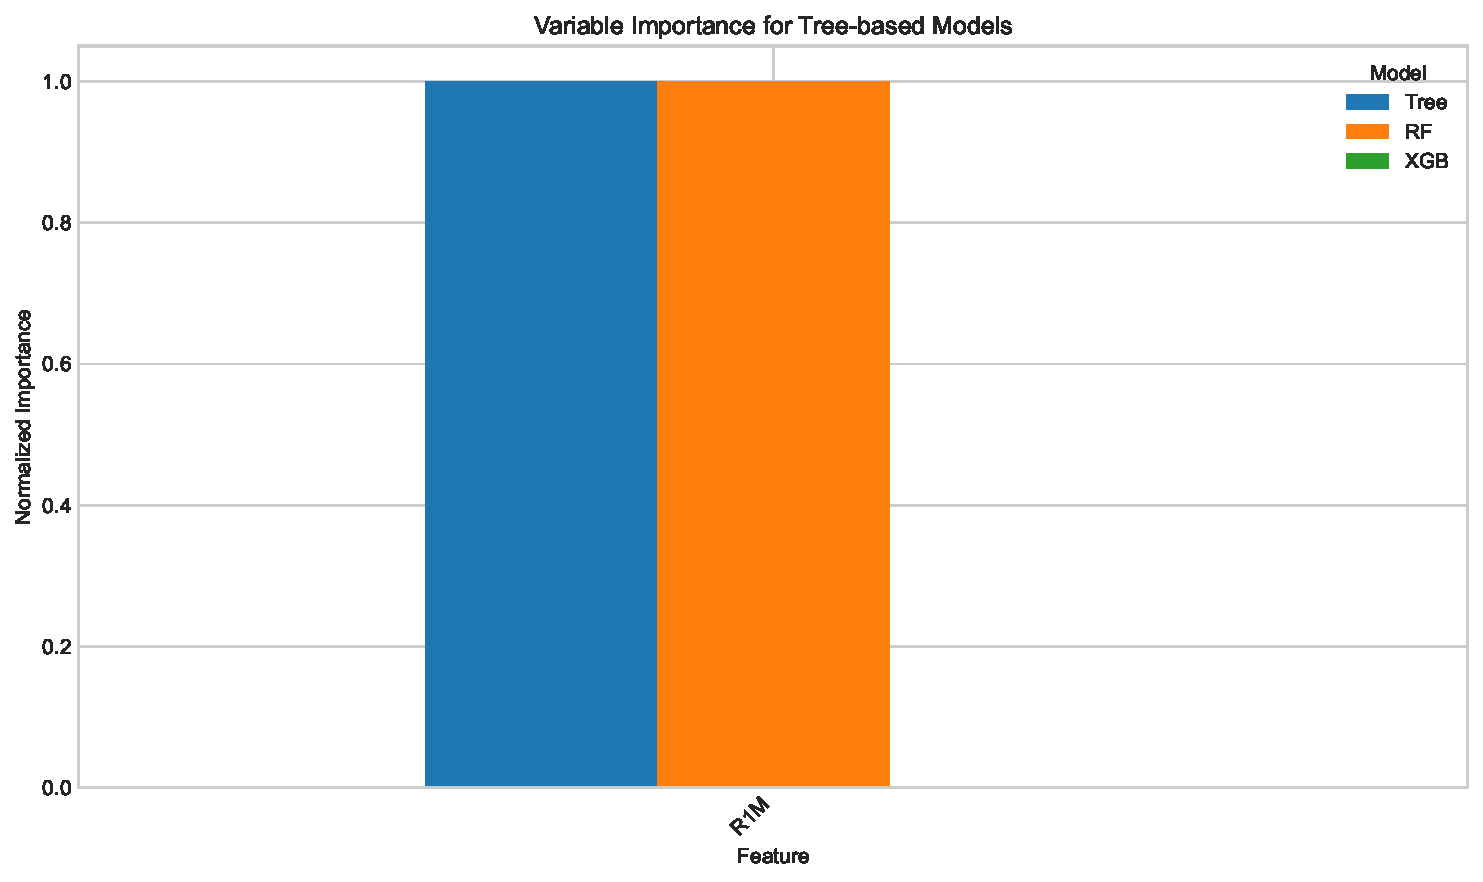
\includegraphics[width=0.7\linewidth]{files/a63c35ac9c1de559e5309910bba01baa.pdf}}
\label{fig-VItrees}
\end{figure}

Given the way the graph is coded, the figure is in fact misleading. Indeed, by construction, the simple tree model only has a small number of features with nonzero importance. In contrast, because random forest and boosted trees are much more complex, they give some importance to many predictors. The graph shows the variables related to the simple tree model only. For scale reasons, the normalization is performed \textit{after} the subset of features is chosen. We preferred to limit the number of features shown on the graph for obvious readability concerns.

There are differences in the way the models rely on the features. For instance, the most important feature changes from a model to the other.

One defining property of random forests is that they give a chance to all features. Indeed, by randomizing the choice of predictors, each individual exogenous variable has a shot at explaining the label. Along with boosted trees, the allocation of importance is more balanced across predictors, compared to the simple tree which puts most of its eggs in just a few baskets.

\paragraph{Variable importance (agnostic)}

The idea of quantifying the importance of each feature in the learning process can be extended to nontree-based models. We refer to the papers mentioned in the study by \cite{fisher2018all} for more information on this stream of the literature. The premise is the same as above: the aim is to quantify to what extent one feature contributes to the learning process.

One way to track the added value of one particular feature is to look at what happens if its values inside the training set are entirely shuffled. If the original feature plays an important role in the explanation of the dependent variable, then the shuffled version of the feature will lead to a much higher loss.

The baseline method to assess feature importance in the general case is the following:

\begin{enumerate}
\item Train the model on the original data and compute the associated loss $l^*$.
\item For each feature $k$, create a new training dataset in which the feature's values are randomly permuted. Then, evaluate the loss $l_k$ of the model based on this altered sample.
\item Rank the variable importance of each feature, computed as a difference $\text{VI}_k=l_k -l^*$ or a ratio $\text{VI}_k=l_k/l^*$.
\end{enumerate}

Whether to compute the losses on the training set or the testing set is an open question and remains to the appreciation of the analyst.
The above procedure is of course random and can be repeated so that the importances are averaged over several trials: this improves the stability of the results.

Below, we implement this algorithm manually for a ridge regression model. We start by the first step: computing the loss on the original training sample.

\begin{verbatim}
# Train ridge regression
X_train = training_sample[features].values
y_train = training_sample['R1M'].values

fit_ridge = Ridge(alpha=0.01)
fit_ridge.fit(X_train, y_train)

# Compute baseline loss
l_star = np.mean((y_train - fit_ridge.predict(X_train))**2)
print(f"Baseline MSE: {l_star:.6f}")
\end{verbatim}

\begin{verbatim}
Baseline MSE: 0.000000
\end{verbatim}

Next, we evaluate the loss when each of the predictors has been sequentially shuffled. To reduce computation time, we only make one round of shuffling.

\begin{verbatim}
# Get the features that appeared in the tree model
selected_features = tree_vi.index.tolist()

# Compute loss for each shuffled feature
losses = []
for feat_name in selected_features:
    temp_data = training_sample[features].copy()
    # Shuffle the feature values
    temp_data[feat_name] = np.random.permutation(temp_data[feat_name].values)
    X_temp = temp_data.values
    loss = np.mean((y_train - fit_ridge.predict(X_temp))**2)
    losses.append(loss)
\end{verbatim}

Finally, we plot the results.

\begin{figure}[!htbp]
\centering
\begin{verbatim}
# Create dataframe with importance (loss increase)
vi_ridge = pd.DataFrame({
    'Feature': selected_features,
    'Importance': np.array(losses) - l_star
})

# Plot
plt.figure(figsize=(10, 6))
plt.bar(vi_ridge['Feature'], vi_ridge['Importance'])
plt.xlabel('Feature')
plt.ylabel('Loss Increase (MSE)')
plt.title('Variable Importance for Ridge Regression (Permutation-based)')
plt.xticks(rotation=45, ha='right')
plt.tight_layout()
plt.show()
\end{verbatim}
\caption[]{Variable importance for a ridge regression model.

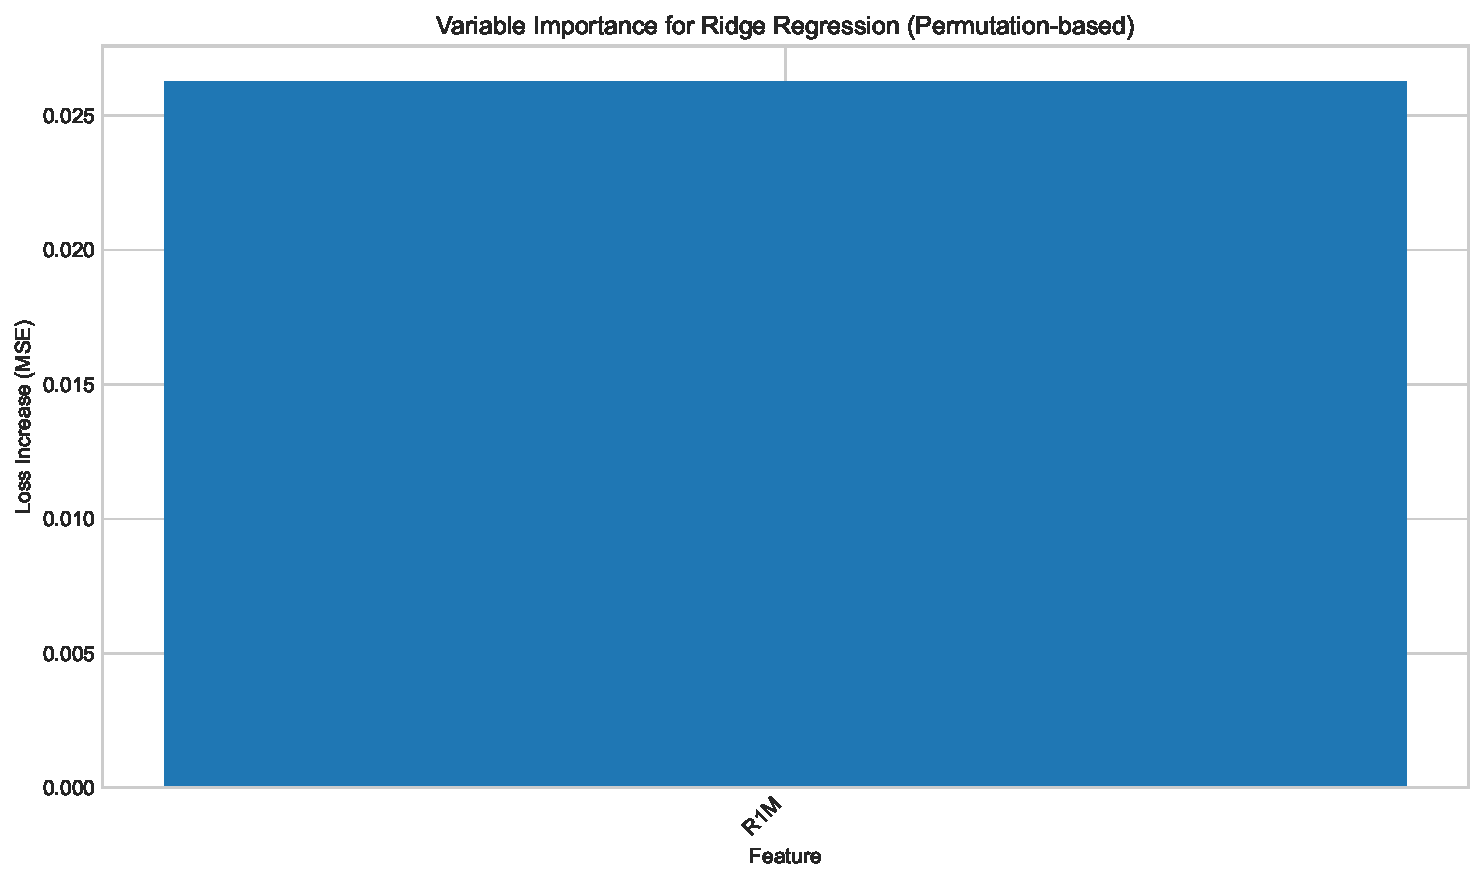
\includegraphics[width=0.7\linewidth]{files/560a7c270fdc4cccecb7c07bb13bf8eb.pdf}}
\label{fig-VIglobal}
\end{figure}

The resulting importances are in line with those of the tree-based models: the most prominent variables closely match the variables from the previous figure. Note that in some cases, the score can even be negative, which means that the predictions are more accurate than the baseline model when the values of the predictor are shuffled!

\paragraph{Partial dependence plot}

Partial dependence plots (PDPs) aim at showing the relationship between the output of a model and the value of a feature (we refer to section 8.2 of \cite{friedman2001greedy} for an early treatment of this subject).

Let us fix a feature $k$. We want to understand the \textbf{average impact} of $k$ on the predictions of the trained model $\hat{f}$. In order to do so, we assume that the feature space is random and we split it in two: $k$ versus $-k$, which stands for all features except for $k$. The partial dependence plot is defined as

\begin{equation}
\label{eq:pdp}
\bar{f}_k(x_k)=\mathbb{E}[\hat{f}(\textbf{x}_{-k},x_k)]=\int \hat{f}(\textbf{x}_{-k},x_k)d\mathbb{P}_{-k}(\textbf{x}_{-k}),
\end{equation}

where $d\mathbb{P}_{ -k}(\cdot)$ is the (multivariate) distribution of the non-$k$ features $\textbf{x}_{ -k}$. The above function takes the feature values $x_k$ as argument and keeps all other features frozen via their sample distributions: this shows the impact of feature $k$ solely. In practice, the average is evaluated using Monte-Carlo simulations:

\begin{equation}
\label{eq:pdpMC}
\bar{f}_k(x_k)\approx \frac{1}{M}\sum_{m=1}^M\hat{f}\left(x_k,\textbf{x}_{-k}^{(m)}\right),
\end{equation}

where $\textbf{x}_{ -k}^{(m)}$ are independent samples of the non-$k$ features.

Theoretically, PDPs could be computed for more than one feature at a time. In practice, this is only possible for two features (yielding a 3D surface) and is more computationally intense.

We illustrate this concept below, using sklearn's \texttt{PartialDependenceDisplay}. The model we seek to explain is the random forest built earlier. We choose to test the impact of the price-to-book ratio on the outcome of the model.

\begin{figure}[!htbp]
\centering
\begin{verbatim}
# Find the index of PB feature
pb_idx = features.index('PB')

# Create partial dependence plot
fig, ax = plt.subplots(figsize=(8, 6))
PartialDependenceDisplay.from_estimator(
    fit_RF,
    training_sample[features],
    features=[pb_idx],
    feature_names=features,
    ax=ax
)
plt.title('Partial Dependence Plot for PB (Price-to-Book)')
plt.tight_layout()
plt.show()
\end{verbatim}
\caption[]{Partial dependence plot for the price-to-book ratio on the random forest model.

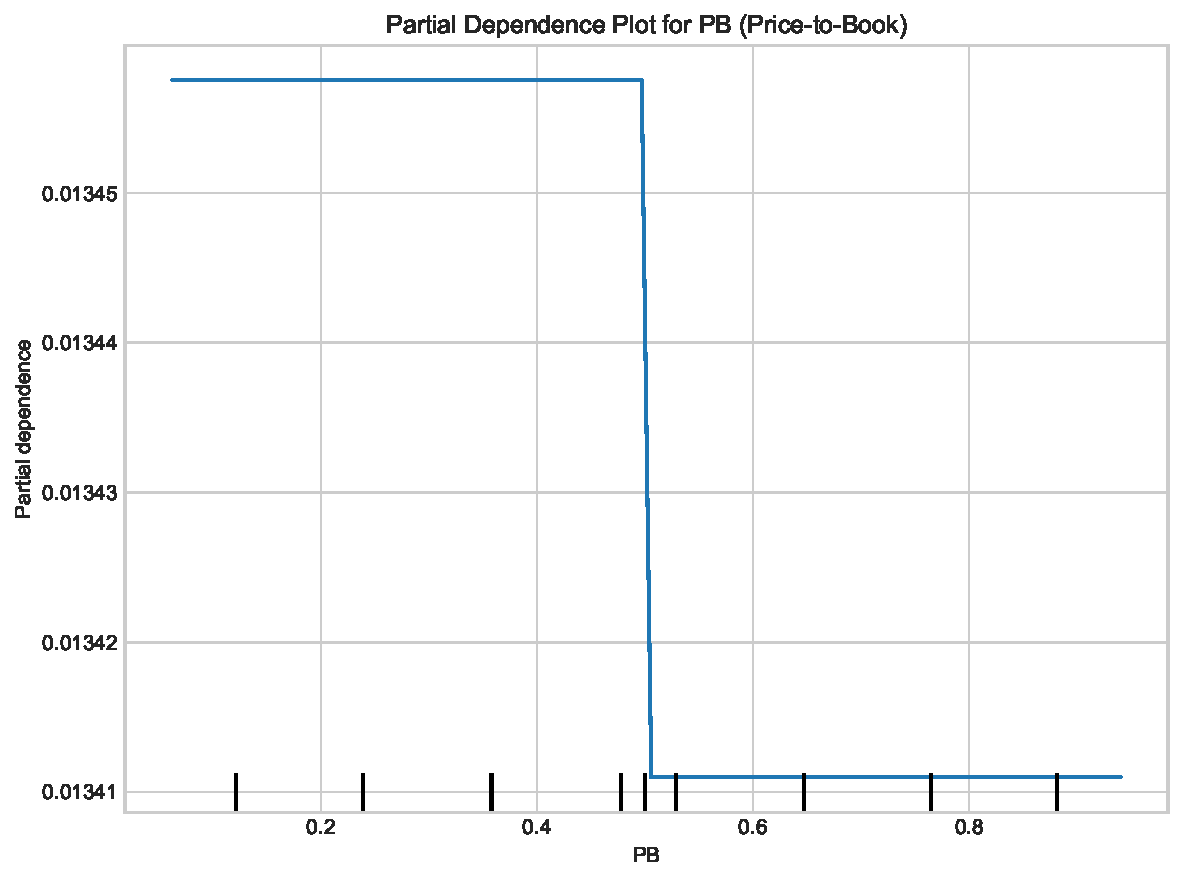
\includegraphics[width=0.7\linewidth]{files/8938e88cead059e1f28fa173a17dbf2c.pdf}}
\label{fig-pdp}
\end{figure}

The average impact of the price-to-book ratio on the predictions is decreasing. This was somewhat expected, given the conditional average of the dependent variable given the price-to-book ratio. When the price-to-book ratio is low, firms are undervalued. Hence, their higher returns are in line with the \textit{value} premium.

Finally, we refer to \cite{zhao2019causal} for a theoretical discussion on the \textit{causality} property of PDPs. Indeed, a deep look at the construction of the PDPs suggests that they could be interpreted as a causal representation of the feature on the model's output.

\subsubsection{Local interpretations}

Whereas global interpretations seek to assess the impact of features on the output \textit{overall}, local methods try to quantify the behavior of the model on particular instances or the neighborhood thereof. Local interpretability has recently gained traction and many papers have been published on this topic. Below, we outline the most widespread methods.

\paragraph{LIME}

LIME (Local Interpretable Model-Agnostic Explanations) is a methodology originally proposed by \cite{ribeiro2016should}. Their aim is to provide a faithful account of the model under two constraints:

\begin{itemize}
\item \textbf{simple interpretability}, which implies a limited number of variables with visual or textual representation. This is to make sure any human can easily understand the outcome of the tool;
\item \textbf{local faithfulness}: the explanation holds for the vicinity of the instance.
\end{itemize}

The original (black-box) model is $f$ and we assume we want to approximate its behavior around instance $x$ with the interpretable model $g$. The simple function $g$ belongs to a larger class $G$. The vicinity of $x$ is denoted $\pi_x$ and the complexity of $g$ is written $\Omega(g)$. LIME seeks an interpretation of the form

\begin{equation}
\xi(x)=\underset{g \in G}{\text{argmin}} \, \mathcal{L}(f,g,\pi_x)+\Omega(g),
\end{equation}

where $\mathcal{L}(f,g,\pi_x)$ is the loss function (error/imprecision) induced by $g$ in the vicinity $\pi_x$ of $x$. The penalization $\Omega(g)$ is for instance the number of leaves or depth of a tree, or the number of predictors in a linear regression.

It now remains to define some of the above terms. The vicinity of $x$ is defined by $\pi_x(z)=e^{ -D(x,z)^2/\sigma^2},$ where $D$ is some distance measure and $\sigma^2$ some scaling constant. We underline that this function decreases when $z$ shifts away from $x$.

The tricky part is the loss function. In order to minimize it, LIME generates artificial samples close to $x$ and averages/sums the error on the label that the simple representation makes. For simplicity, we assume a scalar output for $f$, hence the formulation is the following:

\begin{equation}
\mathcal{L}(f,g,\pi_x)=\sum_z \pi_x(z)(f(z)-g(z))^2
\end{equation}

and the errors are weighted according to their distance from the initial instance $x$: the closest points get the largest weights. In its most basic implementation, the set of models $G$ consists of all linear models.

\begin{figure}[!htbp]
\centering
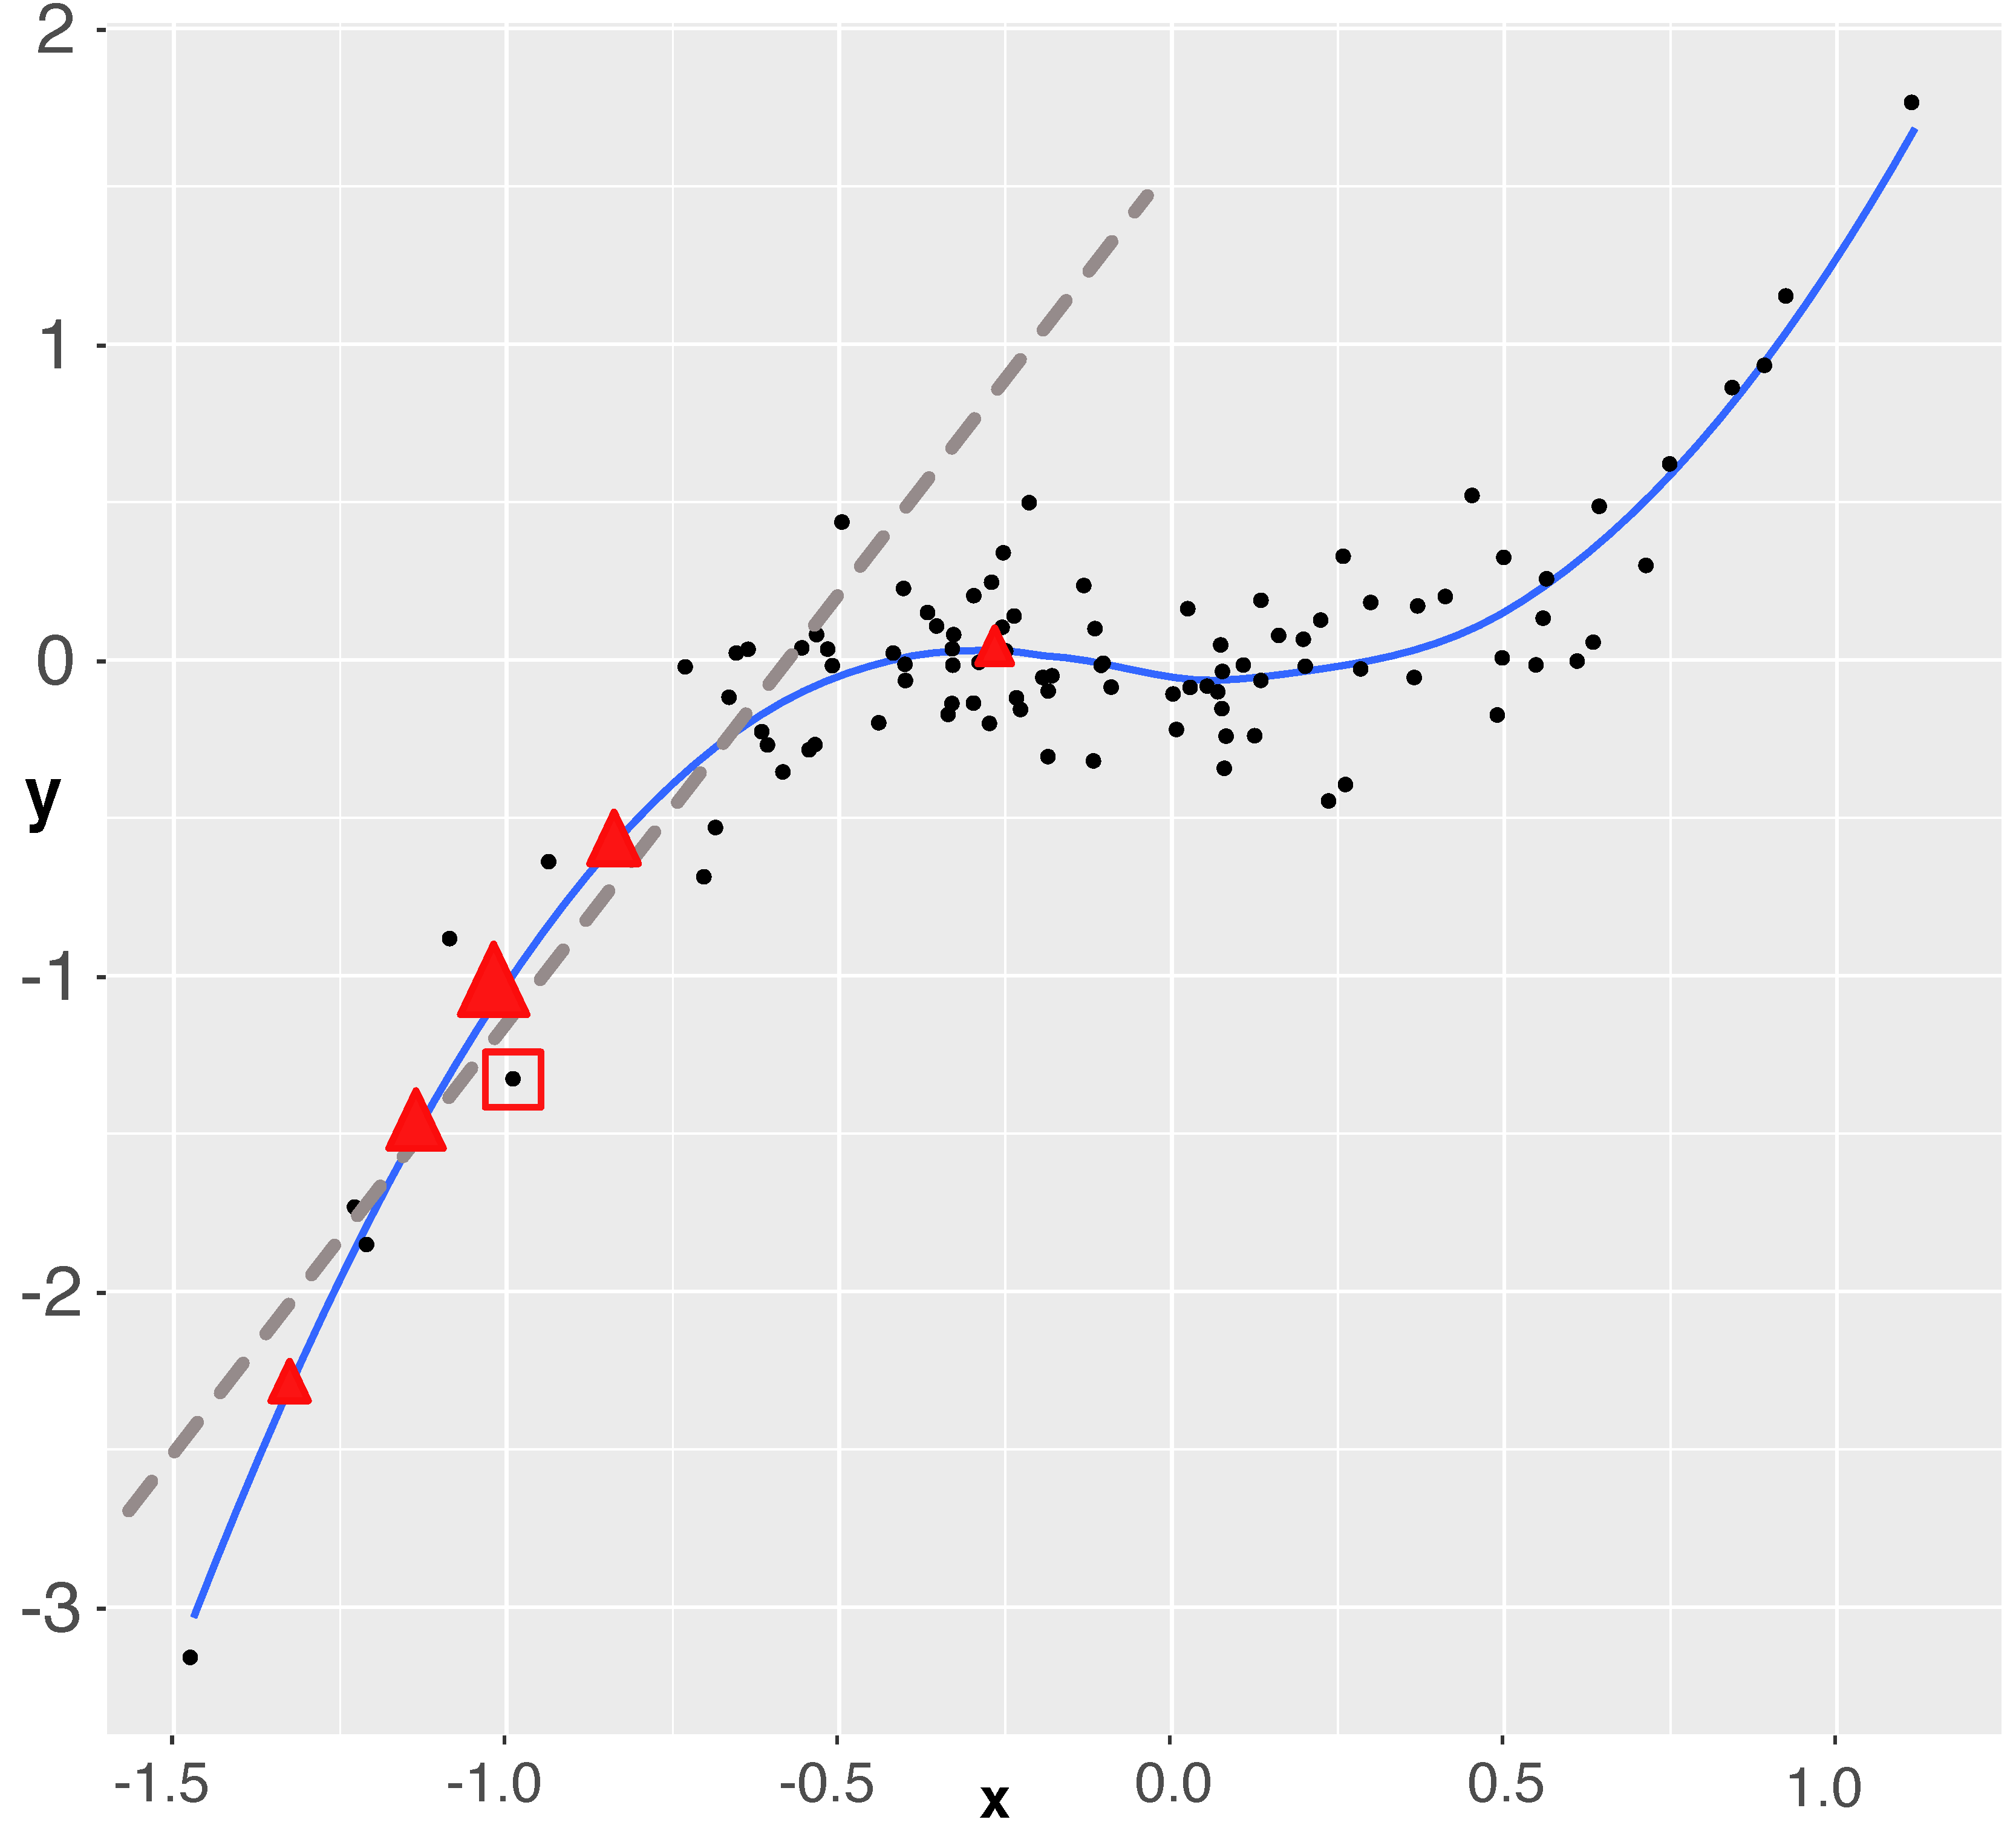
\includegraphics[width=0.7\linewidth]{files/lime-b5024fe6e6e8048b636e5f7966797589.pdf}
\caption[]{Simplistic explanation of LIME: the explained instance is surrounded by a red square. Five points are generated (the triangles) and a weighted linear model is fitted accordingly (dashed grey line).}
\label{fig-lime}
\end{figure}

For expositional clarity, we work with only one dependent variable. The original training sample is shown with the black points. The fitted (trained) model is represented with the blue line (smoothed conditional average) and we want to approximate how the model works around one particular instance which is highlighted by the red square around it. In order to build the approximation, we sample 5 new points around the instance (the 5 red triangles). Each triangle lies on the blue line (they are model predictions) and has a weight proportional to its size: the triangle closest to the instance has a bigger weight. Using weighted least-squares, we build a linear model that fits to these 5 points (the dashed grey line). This is the outcome of the approximation. It gives the two parameters of the model: the intercept and the slope. Both can be evaluated with standard statistical tests.

The sign of the slope is important. It is fairly clear that if the instance had been taken closer to $x=0$, the slope would have probably been almost flat and hence the predictor could be locally discarded. Another important detail is the number of sample points. In our explanation, we take only five, but in practice, a robust estimation usually requires around one thousand points or more. Indeed, when too few neighbors are sampled, the estimation risk is high and the approximation may be rough.

We proceed with an example of implementation. There are several steps:

\begin{enumerate}
\item Fit a model on some training data.
\item Wrap everything using the lime explainer.
\item Focus on a few predictors and see their impact over a few particular instances.
\end{enumerate}

We start with the first step. This time, we work with a boosted tree model.

\begin{verbatim}
import lime
import lime.lime_tabular

# Train XGBoost model with sklearn interface for LIME compatibility
from xgboost import XGBRegressor

xgb_model = XGBRegressor(
    max_depth=5,
    learning_rate=0.5,
    gamma=0.1,
    colsample_bytree=1,
    min_child_weight=10,
    subsample=1,
    n_estimators=10,
    random_state=42
)
xgb_model.fit(training_sample[features_short], training_sample['R1M'])
\end{verbatim}

\begin{verbatim}
XGBRegressor(base_score=None, booster=None, callbacks=None,
             colsample_bylevel=None, colsample_bynode=None, colsample_bytree=1,
             device=None, early_stopping_rounds=None, enable_categorical=False,
             eval_metric=None, feature_types=None, feature_weights=None,
             gamma=0.1, grow_policy=None, importance_type=None,
             interaction_constraints=None, learning_rate=0.5, max_bin=None,
             max_cat_threshold=None, max_cat_to_onehot=None,
             max_delta_step=None, max_depth=5, max_leaves=None,
             min_child_weight=10, missing=nan, monotone_constraints=None,
             multi_strategy=None, n_estimators=10, n_jobs=None,
             num_parallel_tree=None, ...)
\end{verbatim}

Then, we head on to steps two and three. We resort to the \texttt{LimeTabularExplainer} class.

\begin{figure}[!htbp]
\centering
\begin{verbatim}
# Create LIME explainer
explainer = lime.lime_tabular.LimeTabularExplainer(
    training_sample[features_short].values,
    feature_names=features_short,
    mode='regression'
)

# Explain first two instances
fig, axes = plt.subplots(2, 1, figsize=(10, 10))

for i, ax in enumerate(axes):
    instance = training_sample[features_short].iloc[i].values
    explanation = explainer.explain_instance(
        instance,
        xgb_model.predict,
        num_features=6,
        num_samples=900
    )
    
    # Extract feature importance
    exp_list = explanation.as_list()
    features_exp = [x[0] for x in exp_list]
    weights = [x[1] for x in exp_list]
    colors = ['blue' if w > 0 else 'red' for w in weights]
    
    ax.barh(features_exp, weights, color=colors)
    ax.set_xlabel('Weight')
    ax.set_title(f'LIME Explanation for Instance {i+1}')
    ax.axvline(x=0, color='black', linestyle='-', linewidth=0.5)

plt.tight_layout()
plt.show()
\end{verbatim}
\caption[]{LIME explanation for two instances.

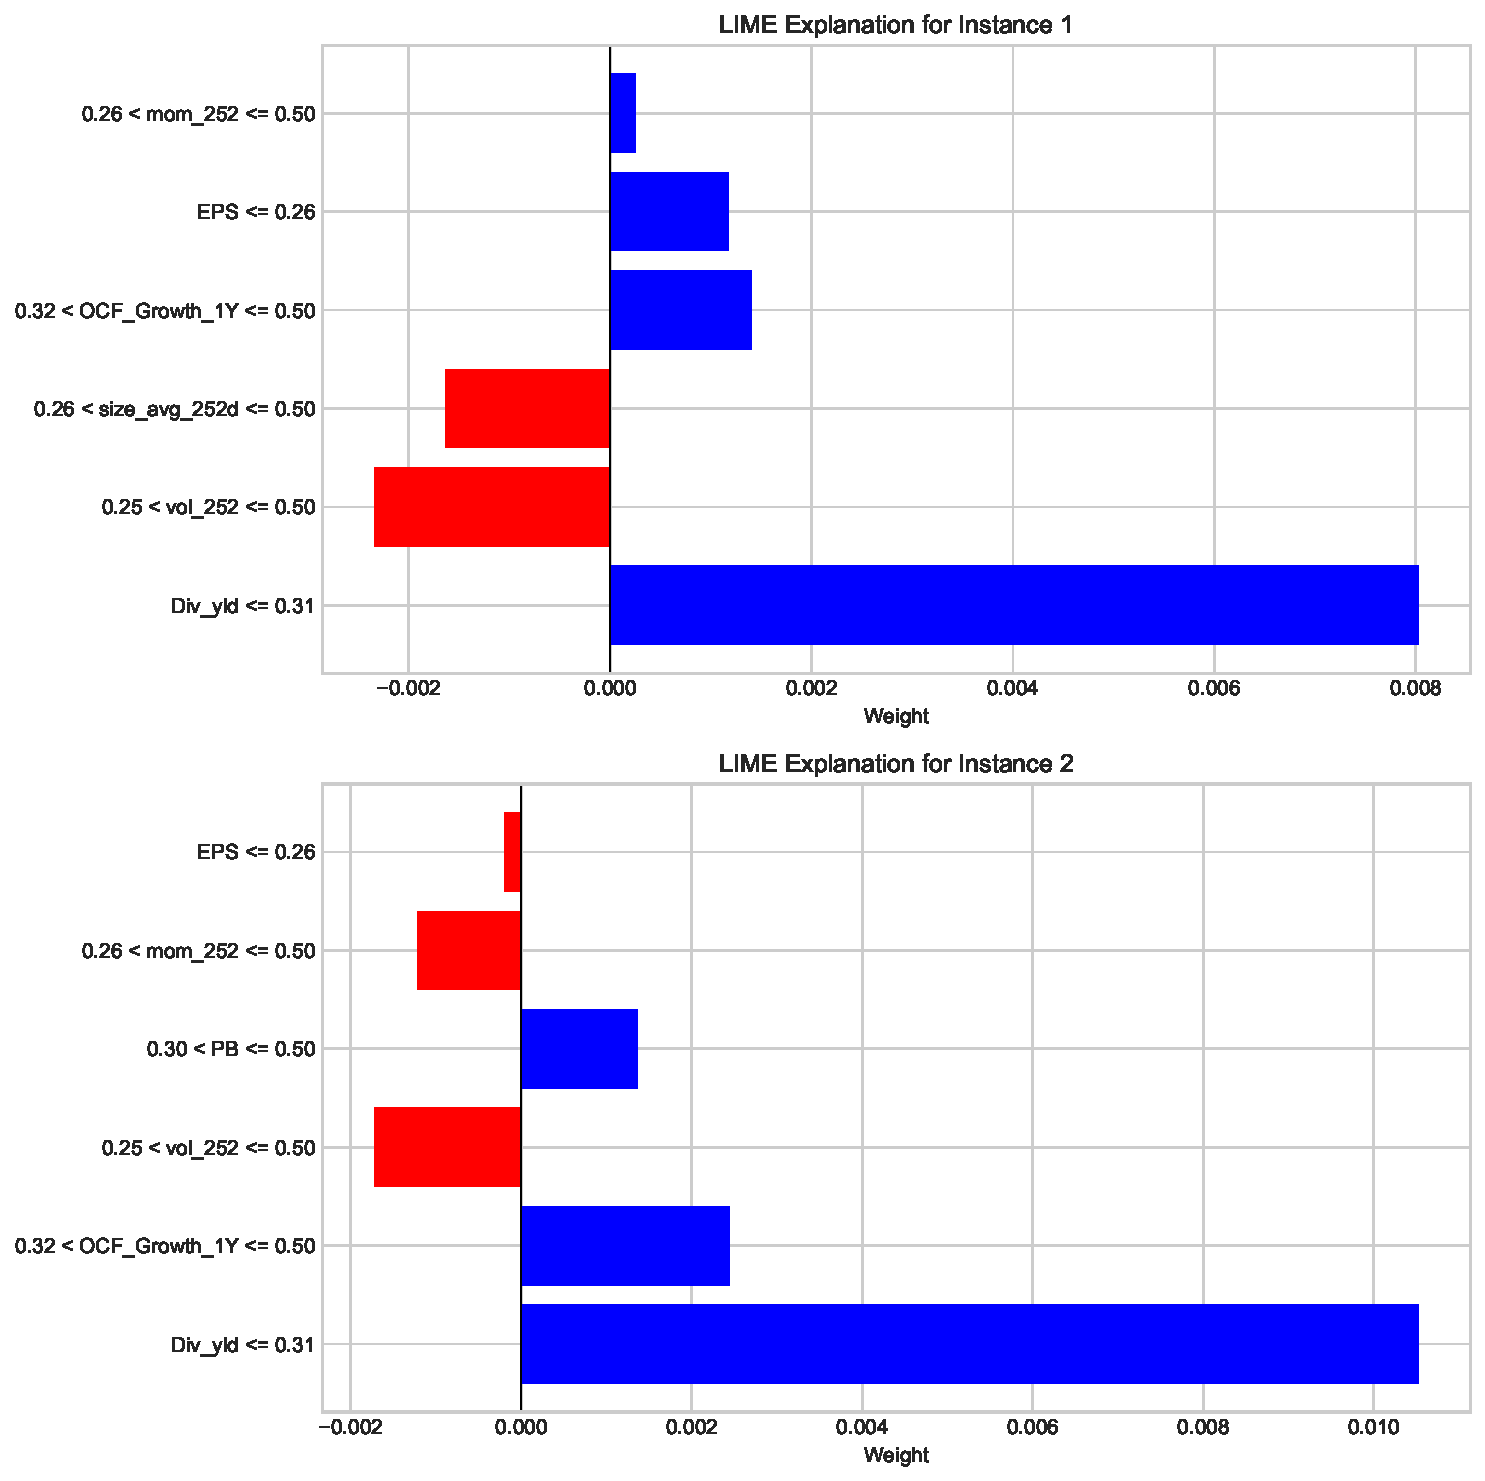
\includegraphics[width=0.7\linewidth]{files/86db60644020eb17540d4eb46ff320e3.pdf}}
\label{fig-lime_output}
\end{figure}

In each graph (one graph corresponds to the explanation around one instance), there are two types of information: the sign of the impact and the magnitude of the impact. The sign is revealed with the color (positive in blue, negative in red) and the magnitude is shown with the size of the bars.

Lastly, we briefly discuss the choice of distance function. It is used to evaluate the discrepancy between the true instance and a simulated one to give more or less weight to the prediction of the sampled instance. Our dataset comprises only numerical data; hence, the Euclidean distance is a natural choice:

\begin{equation}
\text{Euclidean}(\textbf{x}, \textbf{y})=\sqrt{\sum_{n=1}^N(x_n-y_n)^2}.
\end{equation}

Another possible choice would be the Manhattan distance:

\begin{equation}
\text{Manhattan}(\textbf{x}, \textbf{y})=\sum_{n=1}^N|x_n-y_n|.
\end{equation}

The problem with these two distances is that they fail to handle categorical variables. This is where the Gower distance steps in \citep{gower1971general}. The distance imposes a different treatment on features of different types (classes versus numbers essentially, but it can also handle missing data!). For categorical features, the Gower distance applies a binary treatment: the value is equal to 1 if the features are equal, and to zero if not (i.e., $1_{\{x_n=y_n\}}$). For numerical features, the spread is quantified as $1 -\frac{|x_n -y_n|}{R_n}$, where $R_n$ is the maximum absolute value the feature can take. All similarity measurements are then aggregated to yield the final score. Note that in this case, the logic is reversed: $\textbf{x}$ and $\textbf{y}$ are very close if the Gower distance is close to one, and they are far away if the distance is close to zero.

\paragraph{Shapley values}

The approach of Shapley values is somewhat different compared to LIME and closer in spirit to PDPs. It originates from cooperative game theory \citep{shapley1953value}. The rationale is the following. One way to assess the impact (or usefulness) of a variable is to look at what happens if we remove this variable from the dataset. If this is very detrimental to the quality of the model (i.e., to the accuracy of its predictions), then it means that the variable is substantially valuable.

Shapley values have been used to attribute risk or performance of portfolios in \cite{shalit2020shapley} and \cite{moehle2021portfolio}.

Numerically, the simplest way to proceed is to take all variables and remove one to evaluate its predictive ability. Shapley values are computed on a larger scale because they consider all possible combinations of variables to which they add the target predictor. Formally, this gives:

\begin{equation}
\label{eq:shapley}
\phi_k=\sum_{S \subseteq \{x_1,\dots,x_K \} \backslash x_k}\underbrace{\frac{\text{Card}(S)!(K-\text{Card}(S)-1)!}{K!}}_{\text{weight of coalition}}\underbrace{\left(\hat{f}_{S \cup \{x_k\}}(S \cup \{x_k\})-\hat{f}_S(S)\right)}_{\text{gain when adding } x_k}
\end{equation}

$S$ is any subset of the \textbf{coalition} that doesn't include feature $k$ and its size is Card($S$).
In the equation above, the model $f$ must be altered because it's impossible to evaluate $f$ when features are missing. In this case, there are several possible options:

\begin{itemize}
\item set the missing value to its average or median value (in the whole sample) so that its effect is some `average' effect;
\item directly compute an average value $\int_{\mathbb{R}} f(x_1,\dots,x_k,\dots,x_K)d\mathbb{P}_{x_k}$, where $d\mathbb{P}_{x_k}$ is the empirical distribution of $x_k$ in the sample.
\end{itemize}

Obviously, Shapley values can take a lot of time to compute if the number of predictors is large. We refer to \cite{chen2018shapley} for a discussion on a simplifying method that reduces computation times in this case.
Extensions of Shapley values for interpretability are studied in \cite{lundberg2017unified}.

The implementation of Shapley values is permitted in Python via the \texttt{shap} package. There are two restrictions compared to LIME. First, the features must be filtered upfront because all features are shown on the graph (which becomes illegible beyond 20 features). This is why in the code below, we use the short list of predictors.
Second, instances are analyzed one at a time.

We start by fitting a random forest model on the short features.

\begin{verbatim}
import shap

# Train random forest on short features
fit_RF_short = RandomForestRegressor(
    n_estimators=40,
    max_samples=10000,
    bootstrap=True,
    min_samples_leaf=250,
    max_features=4,
    random_state=42
)
fit_RF_short.fit(training_sample[features_short], training_sample['R1M'])
\end{verbatim}

\begin{verbatim}
RandomForestRegressor(max_features=4, max_samples=10000, min_samples_leaf=250,
                      n_estimators=40, random_state=42)
\end{verbatim}

We can then analyze the behavior of the model around the first instance of the training sample.

\begin{figure}[!htbp]
\centering
\begin{verbatim}
# Create SHAP explainer
explainer_shap = shap.TreeExplainer(fit_RF_short)

# Compute SHAP values for the first instance
shap_values = explainer_shap.shap_values(training_sample[features_short].iloc[0:1])

# Plot waterfall for the first instance
shap.initjs()
plt.figure(figsize=(10, 6))
shap.plots.bar(
    shap.Explanation(
        values=shap_values[0],
        base_values=explainer_shap.expected_value,
        feature_names=features_short
    )
)
plt.title('Shapley Values for First Instance')
plt.tight_layout()
plt.show()
\end{verbatim}
\caption[]{Illustration of the Shapley method.


\includegraphics[width=0.7\linewidth]{files/5f4e60dc4dd6eb41c2b750bde9b5b67b.png}

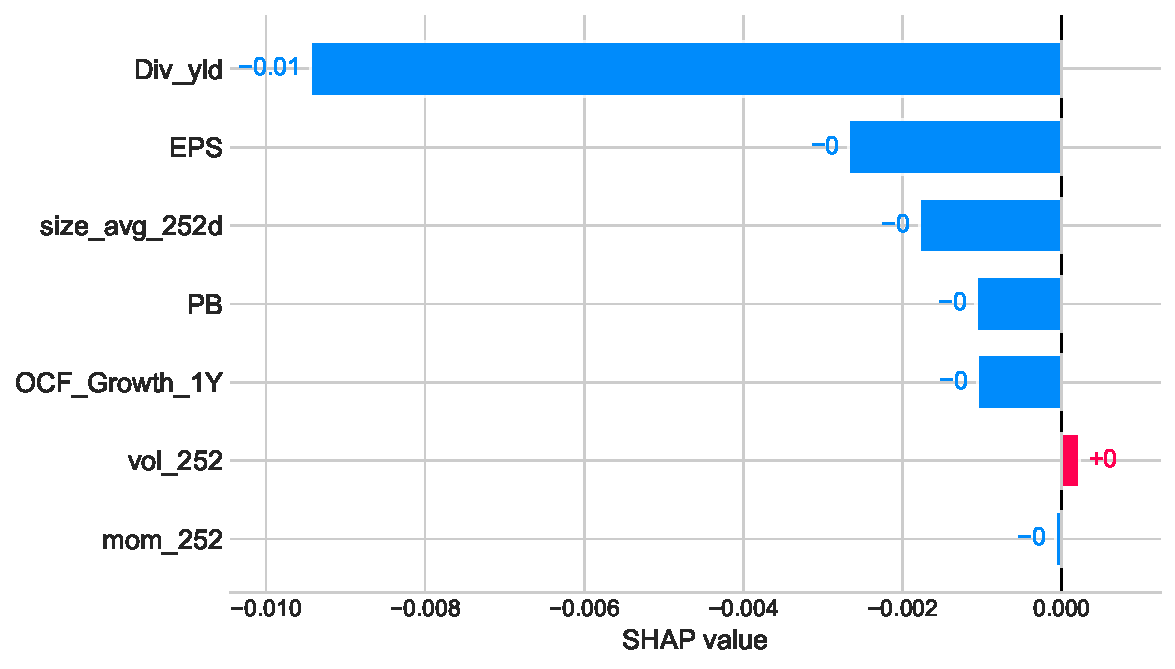
\includegraphics[width=0.7\linewidth]{files/b40cbad58b0872bd8bb1e7bfd709401d.pdf}

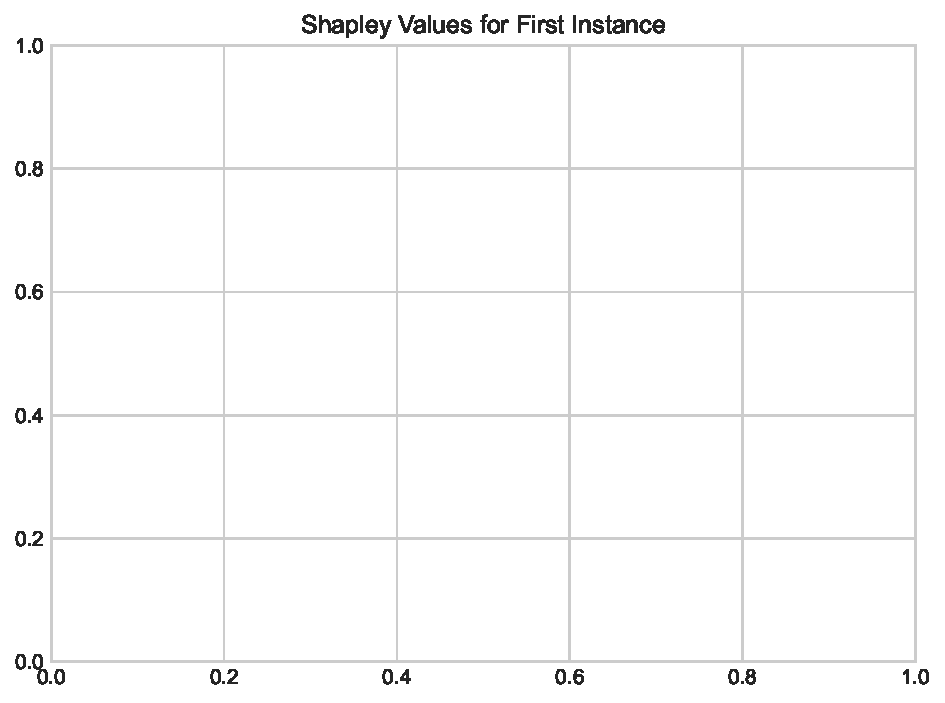
\includegraphics[width=0.7\linewidth]{files/ef0e6757ee3fb1c62d730f579180a991.pdf}}
\label{fig-shapley}
\end{figure}

In the output shown in the figure, we again obtain the two crucial insights: \textbf{sign} of the impact of the feature and \textbf{relative importance} (compared to other features).

\paragraph{Breakdown}

Breakdown (see, e.g., \cite{staniak2018explanations}) is a mixture of ideas from PDPs and Shapley values. The core of breakdown is the so-called \textbf{relaxed model prediction} defined in Equation \ref{eq:breakdown}. It is close in spirit to Equation \ref{eq:pdp}. The difference is that we are working at the local level, i.e., on one particular observation, say $x^*$. We want to measure the impact of a set of predictors on the prediction associated to $x^*$; hence, we fix two sets $\textbf{k}$ (fixed features) and $-\textbf{k}$ (free features) and evaluate a \textbf{proxy} for the average prediction of the estimated model $\hat{f}$ when the set $\textbf{k}$ of predictors is fixed at the values of $x^*$, that is, equal to $x^*_{\textbf{k}}$ in the expression below:

\begin{equation}
\label{eq:breakdown}
\tilde{f}_{\textbf{k}}(x^*)=\frac{1}{M}\sum_{m=1}^M \hat{f}\left(x^{(m)}_{-\textbf{k}},x^*_{\textbf{k}} \right).
\end{equation}

The $x^{(m)}$ in the above expression are either simulated values of instances or simply sampled values from the dataset. The notation implies that the instance has some values replaced by those of $x^*$, namely those that correspond to the indices $\textbf{k}$. When $\textbf{k}$ consists of all features, then $\tilde{f}_{\textbf{k}}(x^*)$ is equal to the raw model prediction $\hat{f}(x^*)$ and when $\textbf{k}$ is empty, it is equal to the average sample value of the label (constant prediction).

The quantity of interest is the so-called contribution of feature $j\notin \textbf{k}$ with respect to data point $x^*$ and set $\textbf{k}$:

\begin{equation}
\phi_{\textbf{k}}^j(x^*)=\tilde{f}_{\textbf{k} \cup j}(x^*)-\tilde{f}_{\textbf{k}}(x^*).
\end{equation}

Just as for Shapley values, the above indicator computes an average impact when augmenting the set of predictors with feature $j$. By definition, it depends on the set $\textbf{k}$, so this is one notable difference with Shapley values (that span \textit{all} permutations). In \cite{staniak2018explanations}, the authors devise a procedure that incrementally increases or decreases the set $\textbf{k}$. This greedy idea helps alleviate the burden of computing all possible combinations of features. Moreover, a very convenient property of their algorithm is that the sum of all contributions is equal to the predicted value:

\begin{equation}
\sum_j \phi_{\textbf{k}}^j(x^*)=f(x^*).
\end{equation}

The visualization makes that very easy to see (as in the figure below).

In order to illustrate one implementation of breakdown, we use SHAP's waterfall plot which provides a similar visualization.

\begin{figure}[!htbp]
\centering
\begin{verbatim}
# Use instance 6 (index 5) for breakdown example
instance_idx = 5
shap_values_instance = explainer_shap.shap_values(training_sample[features_short].iloc[instance_idx:instance_idx+1])

# Create waterfall plot (similar to breakdown)
plt.figure(figsize=(10, 6))
shap.plots.waterfall(
    shap.Explanation(
        values=shap_values_instance[0],
        base_values=explainer_shap.expected_value,
        data=training_sample[features_short].iloc[instance_idx].values,
        feature_names=features_short
    ),
    show=False
)
plt.title(f'Breakdown (Waterfall) for Instance {instance_idx + 1}')
plt.tight_layout()
plt.show()
\end{verbatim}
\caption[]{Example of a breakdown output using SHAP waterfall plot.

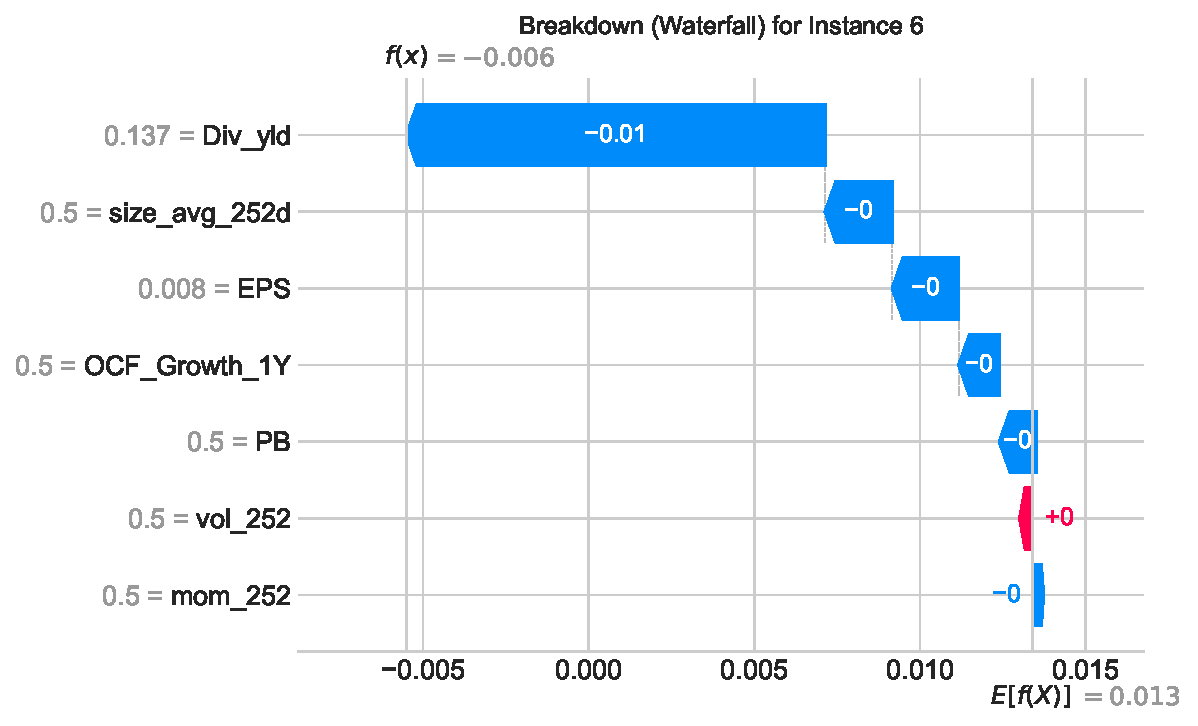
\includegraphics[width=0.7\linewidth]{files/e7646d9fce39070de99a4394500cf3d9.pdf}}
\label{fig-breakdown}
\end{figure}

The graphical output is intuitively interpreted. The base value is the average prediction of the model. Positive contributions push the prediction higher and negative contributions push it lower. The relative sizes indicate the importance of each feature. The final prediction is the sum of the base value and all contributions.

\subsection{Two key concepts: causality and non-stationarity}

A prominent point of criticism faced by ML tools is their inability to uncover \textbf{causality} relationships between features and labels because they are mostly focused (by design) to capture correlations. Correlations are much weaker than causality because they characterize a two-way relationship ($\textbf{X}\leftrightarrow \textbf{y}$), while causality specifies a direction $\textbf{X}\rightarrow \textbf{y}$ or $\textbf{X}\leftarrow \textbf{y}$. One fashionable example is sentiment. Many academic articles seem to find that sentiment (irrespectively of its definition) is a significant driver of future returns. A high sentiment for a particular stock may increase the demand for this stock and push its price up (though contrarian reasonings may also apply: if sentiment is high, it is a sign that mean-reversion is possibly about to happen). The reverse causation is also plausible: returns may well cause sentiment. If a stock experiences a long period of market growth, people become bullish about this stock and sentiment increases (this notably comes from extrapolation, see \cite{barberis2015x} for a theoretical model). In \cite{coqueret2018economic}, it is found (in opposition to most findings in this field), that the latter relationship (returns $\rightarrow$ sentiment) is more likely. This result is backed by causality driven tests (see Section~\ref{sec_granger}).

Statistical causality is a large field and we refer to \cite{pearl2009causality} for a deep dive into this topic. Recently, researchers have sought to link causality with ML approaches (see, e.g., \cite{peters2017elements}, \cite{heinze2018invariant}, \cite{arjovsky2019invariant}). The key notion in their work is \textbf{invariance}.

Often, data is collected not at once, but from different sources at different moments. Some relationships found in these different sources will change, while others may remain the same. The relationships that are invariant to \textbf{changing environments} are likely to stem from (and signal) causality. One counter-example is the following (related in \cite{beery2018recognition}): training a computer vision algorithm to discriminate between cows and camels will lead the algorithm to focus on grass versus sand! This is because most camels are pictured in the desert while cows are shown in green fields of grass. Thus, a picture of a camel on grass will be classified as cow, while a cow on sand would be labelled ``camel''. It is only with pictures of these two animals in different contexts (environments) that the learner will end up truly finding what makes a cow and a camel. A camel will remain a camel no matter where it is pictured: it should be recognized as such by the learner. If so, the representation of the camel becomes invariant over all datasets and the learner has discovered causality, i.e., the true attributes that make the camel a camel (overall silhouette, shape of the back, face, color (possibly misleading!), etc.).

This search for invariance makes sense for many disciplines like computer vision or natural language processing (cats will always look like cats and languages don't change much). In finance, it is not obvious that invariance may exist. Market conditions are known to be time-varying and the relationships between firm characteristics and returns also change from year to year. One solution to this issue may simply be to embrace \textbf{non-stationarity} (see \ref{sec_notations} for a definition of stationarity). In Chapter \href{/chap-15-portfolio-backtesting}{Portfolio backtesting}, we advocate to do that by updating models as frequently as possible with rolling training sets: this allows the predictions to be based on the most recent trends. In Section~\ref{sec_nonstat} below, we introduce other theoretical and practical options.

\subsubsection{Causality}

Traditional machine learning models aim to uncover relationships between variables but do not usually specify \textit{directions} for these relationships. One typical example is the linear regression. If we write $y=a+bx+\epsilon$, then it is also true that $x=b^{ -1}(y -a -\epsilon)$, which is of course also a linear relationship (with respect to $y$). These equations do not define causation whereby $x$ would be a clear determinant of $y$ ($x \rightarrow y$, but the opposite could be false).

Recently, \cite{dacunto2021evolving} have investigated the causal structure of prominent equity factors. The study, via the the VAR-LiNGAM technique of \cite{hyvarinen2010estimation}, finds that risk factor interactions are continuously evolving.

\paragraph{Granger causality}\label{sec_granger}

The most notable tool first proposed by \cite{granger1969investigating} is probably the simplest. For simplicity, we consider only two stationary processes, $X_t$ and $Y_t$. A strict definition of causality could be the following. $X$ can be said to cause $Y$, whenever, for some integer $k$,

\begin{equation}
(Y_{t+1},\dots,Y_{t+k})|(\mathcal{F}_{Y,t}\cup \mathcal{F}_{X,t}) \quad  \overset{d}{\neq} \quad (Y_{t+1},\dots,Y_{t+k})|\mathcal{F}_{Y,t},
\end{equation}

that is, when the distribution of future values of $Y_t$, conditionally on the knowledge of both processes is not the same as the distribution with the sole knowledge of the filtration $\mathcal{F}_{Y,t}$. Hence $X$ does have an impact on $Y$ because its trajectory alters that of $Y$.

Now, this formulation is too vague and impossible to handle numerically, thus we simplify the setting via a linear formulation. We keep the same notations as section 5 of the original paper by \cite{granger1969investigating}. The test consists of two regressions:

\begin{align*}
X_t&=\sum_{j=1}^ma_jX_{t-j}+\sum_{j=1}^mb_jY_{t-j} + \epsilon_t \\
Y_t&=\sum_{j=1}^mc_jX_{t-j}+\sum_{j=1}^md_jY_{t-j} + \nu_t
\end{align*}

where for simplicity, it is assumed that both processes have zero mean. The usual assumptions apply: the Gaussian noises $\epsilon_t$ and $\nu_t$ are uncorrelated in every possible way (mutually and through time). The test is the following: if one $b_j$ is nonzero, then it is said that $Y$ Granger-causes $X$ and if one $c_j$ is nonzero, $X$ Granger-causes $Y$. The two are not mutually exclusive and it is widely accepted that feedback loops can very well occur.

Statistically, under the null hypothesis, $b_1=\dots=b_m=0$ (\textit{resp.} $c_1=\dots=c_m=0$), which can be tested using the usual Fischer distribution. Obviously, the linear restriction can be dismissed but the tests are then much more complex. The main financial article in this direction is \cite{hiemstra1994testing}.

In Python, the \texttt{statsmodels} library provides Granger causality testing. The syntax is straightforward. We test if market capitalization Granger-causes 1 month ahead returns for one particular stock.

\begin{verbatim}
import numpy as np
import pandas as pd
import matplotlib.pyplot as plt
from statsmodels.tsa.stattools import grangercausalitytests
from statsmodels.regression.linear_model import OLS
import statsmodels.api as sm
import warnings
warnings.filterwarnings('ignore')
plt.style.use('seaborn-v0_8-whitegrid')

# Building the data & import functions
from data_build import generate_data
data_ml, features, features_short, returns, stock_ids, stock_ids_short = generate_data()

# Define separation date and create samples
separation_date = "2017-01-15"
training_sample = data_ml[data_ml['date'] <= separation_date].dropna()
testing_sample = data_ml[data_ml['date'] > separation_date].dropna()
\end{verbatim}

\begin{verbatim}
# Get data for first stock
first_stock = training_sample['fsym_id'].unique()[0]
stock_data = training_sample[training_sample['fsym_id'] == first_stock].copy()
stock_data = stock_data.sort_values('date')

# Prepare data for Granger test (needs 2D array with [y, x])
# Test if size_avg_252d (market cap proxy) Granger-causes R1M
granger_data = stock_data[['R1M', 'size_avg_252d']].dropna()

# Perform Granger causality test
# Tests if the second column Granger-causes the first
print("Testing if size_avg_252d Granger-causes R1M:")
print("="*50)
granger_results = grangercausalitytests(granger_data, maxlag=6, verbose=True)
\end{verbatim}

\begin{verbatim}
Testing if size_avg_252d Granger-causes R1M:
==================================================

Granger Causality
number of lags (no zero) 1
ssr based F test:         F=0.2622  , p=0.6096  , df_denom=112, df_num=1
ssr based chi2 test:   chi2=0.2692  , p=0.6039  , df=1
likelihood ratio test: chi2=0.2689  , p=0.6041  , df=1
parameter F test:         F=0.2622  , p=0.6096  , df_denom=112, df_num=1

Granger Causality
number of lags (no zero) 2
ssr based F test:         F=0.1203  , p=0.8867  , df_denom=109, df_num=2
ssr based chi2 test:   chi2=0.2517  , p=0.8817  , df=2
likelihood ratio test: chi2=0.2515  , p=0.8819  , df=2
parameter F test:         F=0.1203  , p=0.8867  , df_denom=109, df_num=2

Granger Causality
number of lags (no zero) 3
ssr based F test:         F=1.2304  , p=0.3024  , df_denom=106, df_num=3
ssr based chi2 test:   chi2=3.9348  , p=0.2686  , df=3
likelihood ratio test: chi2=3.8679  , p=0.2761  , df=3
parameter F test:         F=1.2304  , p=0.3024  , df_denom=106, df_num=3

Granger Causality
number of lags (no zero) 4
ssr based F test:         F=1.2511  , p=0.2942  , df_denom=103, df_num=4
ssr based chi2 test:   chi2=5.4418  , p=0.2449  , df=4
likelihood ratio test: chi2=5.3137  , p=0.2566  , df=4
parameter F test:         F=1.2511  , p=0.2942  , df_denom=103, df_num=4

Granger Causality
number of lags (no zero) 5
ssr based F test:         F=1.0051  , p=0.4188  , df_denom=100, df_num=5
ssr based chi2 test:   chi2=5.5782  , p=0.3495  , df=5
likelihood ratio test: chi2=5.4425  , p=0.3643  , df=5
parameter F test:         F=1.0051  , p=0.4188  , df_denom=100, df_num=5

Granger Causality
number of lags (no zero) 6
ssr based F test:         F=1.0811  , p=0.3792  , df_denom=97, df_num=6
ssr based chi2 test:   chi2=7.3561  , p=0.2892  , df=6
likelihood ratio test: chi2=7.1206  , p=0.3098  , df=6
parameter F test:         F=1.0811  , p=0.3792  , df_denom=97, df_num=6
\end{verbatim}

The test is directional and only tests if $X$ Granger-causes $Y$. In order to test the reverse effect, it is required to reverse the column order. We can also test the reverse direction:

\begin{verbatim}
# Test the reverse: does R1M Granger-cause size_avg_252d?
granger_data_reverse = stock_data[['size_avg_252d', 'R1M']].dropna()
print("\nTesting if R1M Granger-causes size_avg_252d:")
print("="*50)
granger_results_reverse = grangercausalitytests(granger_data_reverse, maxlag=6, verbose=True)
\end{verbatim}

\begin{verbatim}
Testing if R1M Granger-causes size_avg_252d:
==================================================

Granger Causality
number of lags (no zero) 1
ssr based F test:         F=0.0107  , p=0.9178  , df_denom=112, df_num=1
ssr based chi2 test:   chi2=0.0110  , p=0.9165  , df=1
likelihood ratio test: chi2=0.0110  , p=0.9165  , df=1
parameter F test:         F=0.0107  , p=0.9178  , df_denom=112, df_num=1

Granger Causality
number of lags (no zero) 2
ssr based F test:         F=0.0781  , p=0.9250  , df_denom=109, df_num=2
ssr based chi2 test:   chi2=0.1633  , p=0.9216  , df=2
likelihood ratio test: chi2=0.1632  , p=0.9217  , df=2
parameter F test:         F=0.0781  , p=0.9250  , df_denom=109, df_num=2

Granger Causality
number of lags (no zero) 3
ssr based F test:         F=0.0349  , p=0.9912  , df_denom=106, df_num=3
ssr based chi2 test:   chi2=0.1116  , p=0.9904  , df=3
likelihood ratio test: chi2=0.1115  , p=0.9904  , df=3
parameter F test:         F=0.0349  , p=0.9912  , df_denom=106, df_num=3

Granger Causality
number of lags (no zero) 4
ssr based F test:         F=0.0477  , p=0.9956  , df_denom=103, df_num=4
ssr based chi2 test:   chi2=0.2077  , p=0.9950  , df=4
likelihood ratio test: chi2=0.2075  , p=0.9950  , df=4
parameter F test:         F=0.0477  , p=0.9956  , df_denom=103, df_num=4

Granger Causality
number of lags (no zero) 5
ssr based F test:         F=0.3612  , p=0.8739  , df_denom=100, df_num=5
ssr based chi2 test:   chi2=2.0049  , p=0.8485  , df=5
likelihood ratio test: chi2=1.9870  , p=0.8509  , df=5
parameter F test:         F=0.3612  , p=0.8739  , df_denom=100, df_num=5

Granger Causality
number of lags (no zero) 6
ssr based F test:         F=0.4499  , p=0.8435  , df_denom=97, df_num=6
ssr based chi2 test:   chi2=3.0609  , p=0.8012  , df=6
likelihood ratio test: chi2=3.0191  , p=0.8064  , df=6
parameter F test:         F=0.4499  , p=0.8435  , df_denom=97, df_num=6
\end{verbatim}

We nonetheless underline that Granger causality is arguably weaker than the one defined in the next subsection. A process that Granger-causes another one simply contains useful predictive information, which is not proof of causality in a strict sense. Moreover, our test is limited to a linear model and including nonlinearities may alter the conclusion. Lastly, including other regressors (possibly omitted variables) could also change the results (see, e.g., \cite{chow2002multivariate}).

Let us extend this analysis to multiple stocks to get a more robust picture:

\begin{verbatim}
# Test Granger causality across multiple stocks
def test_granger_for_stock(stock_id, data, feature='size_avg_252d', target='R1M', maxlag=4):
    """Test Granger causality for a single stock."""
    stock_data = data[data['fsym_id'] == stock_id].sort_values('date')
    granger_data = stock_data[[target, feature]].dropna()
    
    if len(granger_data) < maxlag + 10:  # Need enough observations
        return None
    
    try:
        results = grangercausalitytests(granger_data, maxlag=maxlag, verbose=False)
        # Get p-value for lag 4
        p_value = results[maxlag][0]['ssr_ftest'][1]
        return p_value
    except:
        return None

# Test on first 50 stocks
stocks_to_test = training_sample['fsym_id'].unique()[:50]
p_values = []
for stock in stocks_to_test:
    p_val = test_granger_for_stock(stock, training_sample)
    if p_val is not None:
        p_values.append(p_val)

# Summary statistics
p_values = np.array(p_values)
print(f"Number of stocks tested: {len(p_values)}")
print(f"Stocks with p-value < 0.05: {np.sum(p_values < 0.05)} ({100*np.mean(p_values < 0.05):.1f}%)")
print(f"Stocks with p-value < 0.10: {np.sum(p_values < 0.10)} ({100*np.mean(p_values < 0.10):.1f}%)")
print(f"Mean p-value: {np.mean(p_values):.4f}")
\end{verbatim}

\begin{verbatim}
Number of stocks tested: 49
Stocks with p-value < 0.05: 16 (32.7%)
Stocks with p-value < 0.10: 23 (46.9%)
Mean p-value: 0.2543
\end{verbatim}

\paragraph{Causal additive models}

The zoo of causal models encompasses a variety of beasts (even BARTs from Section~\ref{BART} are used for this purpose in \cite{hahn2019bayesian}). The interested reader can have a peek at \cite{pearl2009causality}, \cite{peters2017elements}, \cite{maathuis2018handbook} and \cite{hunermund2019causal} and the references therein. One central tool in causal models is the \textbf{do-calculus} developed by Pearl. Whereas traditional probabilities $P[Y|X]$ link the odds of $Y$ conditionally on \textbf{observing} $X$ take some value $x$, the do($\cdot$) \textbf{forces} $X$ to take value $x$. This is a \textit{looking} versus \textit{doing} dichotomy. One classical example is the following. Observing a barometer gives a clue what the weather will be because high pressures are more often associated with sunny days:

\begin{equation}
P[\text{sunny weather}|\text{barometer says ``high''} ]>P[\text{sunny weather}|\text{barometer says ``low''} ],
\end{equation}

but if you hack the barometer (force it to display some value),

\begin{equation}
P[\text{sunny weather}|\text{barometer hacked to ``high''} ]=P[\text{sunny weather}|\text{barometer hacked ``low''} ],
\end{equation}

because hacking the barometer will have no impact on the weather. In short notation, when there is an intervention on the barometer, $P[\text{weather}|\text{do(barometer)}]=P[\text{weather}]$. This is an interesting example related to causality. The overarching variable is pressure. Pressure impacts both the weather and the barometer and this joint effect is called confounding. However, it may not be true that the barometer impacts the weather. The interested reader who wants to dive deeper into these concepts should have a closer look at the work of Judea Pearl. Do-calculus is a very powerful theoretical framework, but it is not easy to apply it to any situation or dataset (see for instance the book review \cite{aronow2020book}).

While we do not formally present an exhaustive tour of the theory behind causal inference, we wish to show some practical implementations because they are easy to interpret. It is always hard to single out one type of model in particular so we choose one that can be explained with simple mathematical tools. We start with the simplest definition of a structural causal model (SCM), where we follow here chapter 3 of \cite{peters2017elements}. The idea behind these models is to introduce some hierarchy (i.e., some additional structure) in the model. Formally, this gives

\begin{align*}
X&=\epsilon_X \\
Y&=f(X,\epsilon_Y),
\end{align*}

where the $\epsilon_X$ and $\epsilon_Y$ are independent noise variables. Plainly, a realization of $X$ is drawn randomly and has then an impact on the realization of $Y$ via $f$. Now this scheme could be more complex if the number of observed variables was larger. Imagine a third variable comes in so that

\begin{align*}
X&=\epsilon_X \\
Y&=f(X,\epsilon_Y),\\
Z&=g(Y,\epsilon_Z)
\end{align*}

In this case, $X$ has a causation effect on $Y$ and then $Y$ has a causation effect on $Z$. We thus have the following connections:

\begin{equation}
\begin{array}{ccccccc} X & &&&\\
&\searrow & &&\\
&&Y&\rightarrow&Z. \\
&\nearrow &&\nearrow& \\
\epsilon_Y & &\epsilon_Z
\end{array}
\end{equation}

The above representation is called a graph and graph theory has its own nomenclature, which we very briefly summarize. The variables are often referred to as \textit{vertices} (or \textit{nodes}) and the arrows as \textit{edges}. Because arrows have a direction, they are called \textit{directed} edges. When two vertices are connected via an edge, they are called \textit{adjacent}. A sequence of adjacent vertices is called a \textit{path}, and it is directed if all edges are arrows. Within a directed path, a vertex that comes first is a parent node and the one just after is a child node.

Graphs can be summarized by adjacency matrices. An adjacency matrix $\textbf{A}=A_{ij}$ is a matrix filled with zeros and ones. $A_{ij}=1$ whenever there is an edge from vertex $i$ to vertex $j$. Usually, self-loops ($X \rightarrow X$) are prohibited so that adjacency matrices have zeros on the diagonal. If we consider a simplified version of the above graph like $X \rightarrow Y \rightarrow Z$, the corresponding adjacency matrix is

\begin{equation}
\textbf{A}=\begin{bmatrix}
0 & 1 & 0 \\
0 & 0 & 1 \\
0& 0&0
\end{bmatrix}.
\end{equation}

where letters $X$, $Y$, and $Z$ are naturally ordered alphabetically. There are only two arrows: from $X$ to $Y$ (first row, second column) and from $Y$ to $Z$ (second row, third column).

A \textbf{cycle} is a particular type of path that creates a loop, i.e., when the first vertex is also the last. The sequence $X \rightarrow Y \rightarrow Z \rightarrow X$ is a cycle. Technically, cycles pose problems. To illustrate this, consider the simple sequence $X \rightarrow Y \rightarrow X$. This would imply that a realization of $X$ causes $Y$ which in turn would cause the realization of $Y$. While Granger causality can be viewed as allowing this kind of connection, general causal models usually avoid cycles and work with \textbf{directed acyclic graphs} (DAGs).

Equipped with these tools, we can explicitize a very general form of models:

\begin{equation}
\label{eq:CAM0}
X_j=f_j\left(\textbf{X}_{\text{pa}_D(j)},\epsilon_j  \right),
\end{equation}

where the noise variables are mutually independent. The notation $\text{pa}_D(j)$ refers to the set of parent nodes of vertex $j$ within the graph structure $D$. Hence, $X_j$ is a function of all of its parents and some noise term $\epsilon_j$. An additive causal model is a mild simplification of the above specification:

\begin{equation}
\label{eq:CAM}
X_j=\sum_{k\in \text{pa}_D(j)}f_{j,k}\left(\textbf{X}_{k}  \right)+\epsilon_j,
\end{equation}

where the nonlinear effect of each variable is cumulative, hence the term `\textit{additive}'. Note that there is no time index there. In contrast to Granger causality, there is no natural ordering. Such models are very complex and hard to estimate. The details can be found in \cite{buhlmann2014cam}.

In Python, we can use the \texttt{causal-learn} library (formerly \texttt{causaldag}) which implements various causal discovery algorithms including the PC algorithm. Let's use it to discover the causal structure among our features.

\begin{verbatim}
# Causal discovery using PC algorithm
# Note: This requires the causal-learn library
# pip install causal-learn

try:
    from causallearn.search.ConstraintBased.PC import pc
    from causallearn.utils.GraphUtils import GraphUtils
    
    # Prepare data for causal discovery
    causal_vars = ['R1M'] + features_short
    data_caus = training_sample[causal_vars].dropna().values
    
    # Run PC algorithm
    # alpha is the significance level for conditional independence tests
    cg = pc(data_caus, alpha=0.01, indep_test='fisherz')
    
    # Get the adjacency matrix
    adj_matrix = cg.G.graph
    
    print("Causal Graph Adjacency Matrix:")
    print("Variables:", causal_vars)
    print("\nAdjacency matrix (1 = edge, -1 = directed edge):")
    adj_df = pd.DataFrame(adj_matrix, index=causal_vars, columns=causal_vars)
    print(adj_df)
    
    # Visualize the graph
    print("\nEdge interpretation:")
    print(" 1: undirected edge (A -- B)")
    print("-1: directed edge (A -> B when adj[A,B]=-1 and adj[B,A]=1)")
    
except ImportError:
    print("causal-learn library not installed.")
    print("Install with: pip install causal-learn")
    print("\nFalling back to correlation-based analysis...")
    
    # Alternative: show correlation matrix as proxy
    causal_vars = ['R1M'] + features_short
    data_caus = training_sample[causal_vars].dropna()
    corr_matrix = data_caus.corr()
    print("\nCorrelation matrix (not causal, but informative):")
    print(corr_matrix.round(3))
\end{verbatim}

\begin{verbatim}
0%|          | 0/8 [00:00<?, ?it/s]
\end{verbatim}

\begin{verbatim}
Causal Graph Adjacency Matrix:
Variables: ['R1M', 'Div_yld', 'EPS', 'size_avg_252d', 'mom_252', 'OCF_Growth_1Y', 'PB', 'vol_252']

Adjacency matrix (1 = edge, -1 = directed edge):
               R1M  Div_yld  EPS  size_avg_252d  mom_252  OCF_Growth_1Y  PB  \
R1M              0        0    1             -1        0              0   1   
Div_yld          0        0    1              1        1              0   1   
EPS             -1       -1    0             -1        0             -1   0   
size_avg_252d    1       -1    1              0        1              0   1   
mom_252          0       -1    0             -1        0             -1  -1   
OCF_Growth_1Y    0        0    1              0        1              0   1   
PB              -1       -1    0             -1       -1             -1   0   
vol_252          0        1    1              1        1              1   1   

               vol_252  
R1M                  0  
Div_yld             -1  
EPS                 -1  
size_avg_252d       -1  
mom_252             -1  
OCF_Growth_1Y       -1  
PB                  -1  
vol_252              0  

Edge interpretation:
 1: undirected edge (A -- B)
-1: directed edge (A -> B when adj[A,B]=-1 and adj[B,A]=1)
\end{verbatim}

\paragraph{Modern Causal Inference: DoWhy and Double Machine Learning}

Recent advances in causal inference have led to powerful frameworks that combine causal reasoning with machine learning. Two notable developments are:

\begin{enumerate}
\item \textbf{DoWhy} \citep{sharma2020dowhy}: A Python library that provides a unified interface for causal inference, implementing the four steps of causal analysis: model, identify, estimate, and refute.
\item \textbf{Double Machine Learning (DML)} \citep{chernozhukov2018double}: A method that uses ML to estimate nuisance parameters while maintaining valid inference for causal parameters.
\end{enumerate}

The key insight of DML is to use cross-fitting: split the data, use one part to estimate nuisance functions (like propensity scores or outcome predictions), and use the other part for the final causal estimate. This avoids overfitting bias.

Let's demonstrate a simple causal effect estimation using regression-based methods:

\begin{verbatim}
# Simple causal effect estimation using regression adjustment
# We estimate the effect of a "treatment" (high PB ratio) on returns

from sklearn.linear_model import LinearRegression, LassoCV
from sklearn.model_selection import cross_val_predict

# Define treatment: above median PB ratio
data_causal = training_sample[['R1M', 'PB'] + [f for f in features_short if f != 'PB']].dropna()
data_causal['treatment'] = (data_causal['PB'] > data_causal['PB'].median()).astype(int)

# Confounders (other features that might affect both PB and returns)
confounders = [f for f in features_short if f != 'PB']

# Method 1: Simple difference in means (naive, biased)
treated_mean = data_causal[data_causal['treatment'] == 1]['R1M'].mean()
control_mean = data_causal[data_causal['treatment'] == 0]['R1M'].mean()
naive_effect = treated_mean - control_mean

print("Causal Effect Estimation: High PB vs Low PB on Returns")
print("="*60)
print(f"\n1. Naive difference in means: {naive_effect:.6f}")
print(f"   (Treated mean: {treated_mean:.6f}, Control mean: {control_mean:.6f})")

# Method 2: Regression adjustment (controlling for confounders)
X_reg = data_causal[['treatment'] + confounders]
y_reg = data_causal['R1M']
X_reg = sm.add_constant(X_reg)
model_reg = OLS(y_reg, X_reg).fit()
reg_effect = model_reg.params['treatment']
reg_se = model_reg.bse['treatment']
reg_pvalue = model_reg.pvalues['treatment']

print(f"\n2. Regression adjustment: {reg_effect:.6f} (SE: {reg_se:.6f}, p-value: {reg_pvalue:.4f})")
\end{verbatim}

\begin{verbatim}
Causal Effect Estimation: High PB vs Low PB on Returns
============================================================

1. Naive difference in means: -0.000774
   (Treated mean: 0.012950, Control mean: 0.013724)

2. Regression adjustment: 0.000963 (SE: 0.000505, p-value: 0.0564)
\end{verbatim}

\begin{verbatim}
# Method 3: Double Machine Learning (Partially Linear Model)
# Y = theta * D + g(X) + epsilon
# D = m(X) + eta
# where D is treatment, X are confounders

from sklearn.ensemble import RandomForestRegressor, GradientBoostingRegressor

def double_ml_estimate(Y, D, X, n_splits=5):
    """
    Simple Double Machine Learning estimator.
    
    Y: outcome
    D: treatment
    X: confounders
    """
    n = len(Y)
    
    # Use cross-fitting to get residuals
    from sklearn.model_selection import KFold
    
    kf = KFold(n_splits=n_splits, shuffle=True, random_state=42)
    
    Y_residuals = np.zeros(n)
    D_residuals = np.zeros(n)
    
    for train_idx, test_idx in kf.split(X):
        # Fit outcome model: E[Y|X]
        model_y = GradientBoostingRegressor(n_estimators=50, max_depth=3, random_state=42)
        model_y.fit(X[train_idx], Y[train_idx])
        Y_residuals[test_idx] = Y[test_idx] - model_y.predict(X[test_idx])
        
        # Fit treatment model: E[D|X]
        model_d = GradientBoostingRegressor(n_estimators=50, max_depth=3, random_state=42)
        model_d.fit(X[train_idx], D[train_idx])
        D_residuals[test_idx] = D[test_idx] - model_d.predict(X[test_idx])
    
    # Final stage: regress Y residuals on D residuals
    theta = np.sum(D_residuals * Y_residuals) / np.sum(D_residuals ** 2)
    
    # Standard error (heteroskedasticity-robust)
    residuals = Y_residuals - theta * D_residuals
    V = np.sum(D_residuals ** 2 * residuals ** 2) / (np.sum(D_residuals ** 2) ** 2)
    se = np.sqrt(V * n)
    
    return theta, se

# Apply DML
Y = data_causal['R1M'].values
D = data_causal['treatment'].values
X = data_causal[confounders].values

dml_effect, dml_se = double_ml_estimate(Y, D, X)
dml_tstat = dml_effect / dml_se

print(f"\n3. Double Machine Learning: {dml_effect:.6f} (SE: {dml_se:.6f}, t-stat: {dml_tstat:.2f})")

# Summary
print("\n" + "="*60)
print("Summary: Effect of High PB (value factor) on Returns")
print(f"  Naive:                {naive_effect:.6f}")
print(f"  Regression adjusted:  {reg_effect:.6f}")
print(f"  Double ML:            {dml_effect:.6f}")
\end{verbatim}

\begin{verbatim}
3. Double Machine Learning: -0.002093 (SE: 0.247868, t-stat: -0.01)

============================================================
Summary: Effect of High PB (value factor) on Returns
  Naive:                -0.000774
  Regression adjusted:  0.000963
  Double ML:            -0.002093
\end{verbatim}

The differences between these estimates highlight the importance of proper causal methodology. The naive estimate doesn't account for confounding, while regression adjustment and DML attempt to isolate the true causal effect by controlling for other variables that might influence both the treatment (PB ratio) and the outcome (returns).

\paragraph{Structural time series models}

We end the topic of causality by mentioning a particular type of structural models: \textbf{structural time series}. Because we illustrate their relevance for a particular kind of causal inference, we closely follow the notations of \cite{brodersen2015inferring}. The model is driven by two equations:

\begin{align*}
y_t&=\textbf{Z}_t'\boldsymbol{\alpha}_t+\epsilon_t \\
\boldsymbol{\alpha}_{t+1}& =\textbf{T}_t\boldsymbol{\alpha}_{t}+\textbf{R}_t\boldsymbol{\eta}_t.
\end{align*}

The dependent variable is expressed as a linear function of state variables $\boldsymbol{\alpha}_t$ plus an error term. These variables are in turn linear functions of their past values plus another error term which can have a complex structure (it's a product of a matrix $\textbf{R}_t$ with a centered Gaussian term $\boldsymbol{\eta}_t$). This specification nests many models as special cases, like ARIMA for instance.

The goal of \cite{brodersen2015inferring} is to detect causal impacts via regime changes. They estimate the above model over a given training period and then predict the model's response on some test set. If the aggregate (summed/integrated) error between the realized versus predicted values is significant (based on some statistical test), then the authors conclude that the breaking point is relevant. Originally, the aim of the approach is to quantify the effect of an intervention by looking at how a model trained before the intervention behaves after the intervention.

Below, we test if a particular date point in the sample (e.g., during the 2008 financial crisis) is a turning point. We use the \texttt{causalimpact} Python package which implements the methodology.

\begin{verbatim}
# Causal Impact Analysis - Manual Implementation                                                  
# Since the causalimpact library has compatibility issues, we implement a simpler version         
                                                                                                    
from sklearn.linear_model import BayesianRidge                                                    
import numpy as np                                                                                
                                                                                                    
# Get data for first stock                                                                        
first_stock = data_ml['fsym_id'].unique()[0]                                                      
stock1_data = data_ml[data_ml['fsym_id'] ==                                                       
first_stock].sort_values('date').reset_index(drop=True)                                           
                                                                                                    
# Prepare data                                                                                    
struct_data = stock1_data[['R1M'] + features_short].dropna().reset_index(drop=True)               
                                                                                                    
# Define periods                                                                                  
pre_start, pre_end = 0, 99                                                                        
post_start, post_end = 100, min(199, len(struct_data)-1)                                          
                                                                                                    
if len(struct_data) > post_end:                                                                   
      # Split data                                                                                  
      pre_data = struct_data.iloc[pre_start:pre_end+1]                                              
      post_data = struct_data.iloc[post_start:post_end+1]                                           
                                                                                                    
      # Train model on pre-period to predict Y from covariates                                      
      X_pre = pre_data[features_short].values                                                       
      y_pre = pre_data['R1M'].values                                                                
                                                                                                    
      X_post = post_data[features_short].values                                                     
      y_post = post_data['R1M'].values                                                              
                                                                                                    
      # Fit Bayesian Ridge regression on pre-period                                                 
      model = BayesianRidge()                                                                       
      model.fit(X_pre, y_pre)                                                                       
                                                                                                    
      # Predict counterfactual for post-period                                                      
      y_post_pred, y_post_std = model.predict(X_post, return_std=True)                              
                                                                                                    
      # Compute causal impact                                                                       
      pointwise_effect = y_post - y_post_pred                                                       
      cumulative_effect = np.cumsum(pointwise_effect)                                               
                                                                                                    
      # Summary statistics                                                                          
      avg_effect = pointwise_effect.mean()                                                          
      total_effect = pointwise_effect.sum()                                                         
                                                                                                    
      print("Causal Impact Analysis (Manual Implementation)")                                       
      print("=" * 60)                                                                               
      print(f"\nPre-period:  [{pre_start}, {pre_end}]")                                             
      print(f"Post-period: [{post_start}, {post_end}]")                                             
      print(f"\nPosterior Inference:")                                                              
      print(f"  Average effect:    {avg_effect:.6f}")                                               
      print(f"  Cumulative effect: {total_effect:.6f}")                                             
      print(f"\nActual post-period mean:      {y_post.mean():.6f}")                                 
      print(f"Predicted post-period mean:   {y_post_pred.mean():.6f}")                              
      print(f"Difference (causal effect):   {y_post.mean() - y_post_pred.mean():.6f}")              
                                                                                                    
      # Store for plotting                                                                          
      ci_results = {                                                                                
          'y_post': y_post,                                                                         
          'y_post_pred': y_post_pred,                                                               
          'y_post_std': y_post_std,                                                                 
          'pointwise_effect': pointwise_effect,                                                     
          'cumulative_effect': cumulative_effect                                                    
      }                                                                                             
else:                                                                                             
      print(f"Not enough data: {len(struct_data)} rows (need > {post_end})")
\end{verbatim}

\begin{verbatim}
Causal Impact Analysis (Manual Implementation)
============================================================

Pre-period:  [0, 99]
Post-period: [100, 199]

Posterior Inference:
  Average effect:    -0.005486
  Cumulative effect: -0.548597

Actual post-period mean:      0.018389
Predicted post-period mean:   0.023875
Difference (causal effect):   -0.005486
\end{verbatim}

\begin{figure}[!htbp]
\centering
\begin{verbatim}
fig, axes = plt.subplots(3, 1, figsize=(12, 10))                                                  
                                                                                                    
time_idx = np.arange(len(ci_results['y_post']))                                                   
                                                                                                    
# Plot 1: Actual vs Predicted                                                                     
axes[0].plot(time_idx, ci_results['y_post'], 'b-', label='Actual', linewidth=1.5)                 
axes[0].plot(time_idx, ci_results['y_post_pred'], 'r--', label='Predicted (counterfactual)',      
  linewidth=1.5)                                                                                    
axes[0].fill_between(time_idx,                                                                    
                       ci_results['y_post_pred'] - 1.96*ci_results['y_post_std'],                   
                       ci_results['y_post_pred'] + 1.96*ci_results['y_post_std'],                   
                       alpha=0.2, color='red', label='95% CI')                                      
axes[0].set_ylabel('Returns')                                                                     
axes[0].set_title('Actual vs Counterfactual Prediction')                                          
axes[0].legend()                                                                                  
                                                                                                    
# Plot 2: Pointwise Effect                                                                        
axes[1].plot(time_idx, ci_results['pointwise_effect'], 'g-', linewidth=1.5)                       
axes[1].axhline(y=0, color='black', linestyle='--', linewidth=0.5)                                
axes[1].fill_between(time_idx,                                                                    
                       -1.96*ci_results['y_post_std'],                                              
                       1.96*ci_results['y_post_std'],                                               
                       alpha=0.2, color='green')                                                    
axes[1].set_ylabel('Effect')                                                                      
axes[1].set_title('Pointwise Causal Effect')                                                      
                                                                                                    
# Plot 3: Cumulative Effect                                                                       
axes[2].plot(time_idx, ci_results['cumulative_effect'], 'purple', linewidth=1.5)                  
axes[2].axhline(y=0, color='black', linestyle='--', linewidth=0.5)                                
axes[2].set_xlabel('Time (post-intervention)')                                                    
axes[2].set_ylabel('Cumulative Effect')                                                           
axes[2].set_title('Cumulative Causal Effect')                                                     
                                                                                                    
plt.tight_layout()                                                                                
plt.show()
\end{verbatim}
\caption[]{Causal impact analysis results.

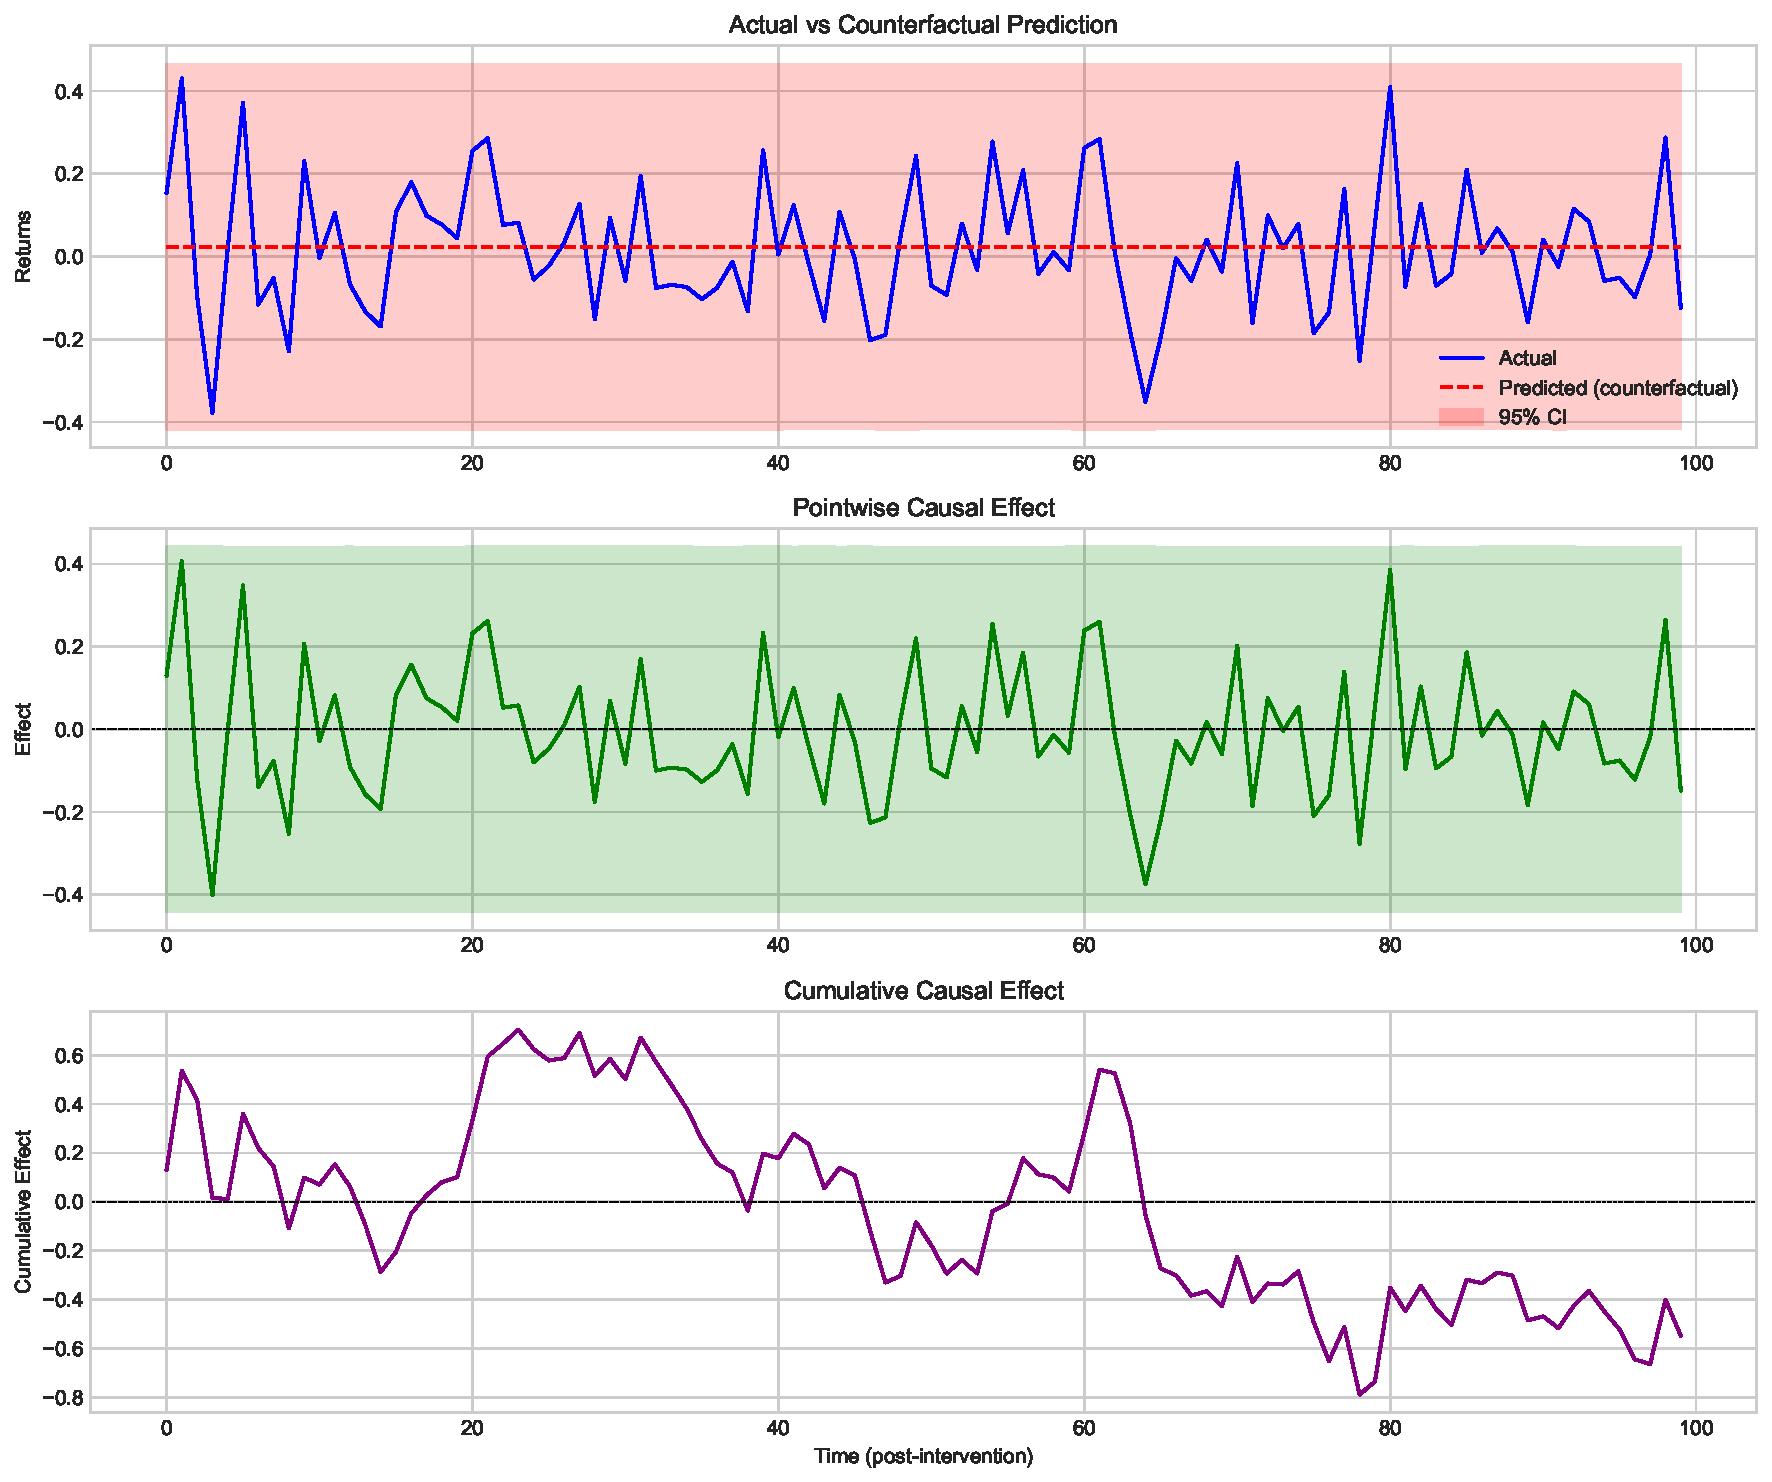
\includegraphics[width=0.7\linewidth]{files/8db47c4c82a53a87d2db7934534432e7.pdf}}
\label{fig-causalimpact}
\end{figure}

\subsubsection{Dealing with changing environments}\label{sec_nonstat}

The most common assumption in machine learning contributions is that the samples that are studied are i.i.d. realizations of a phenomenon that we are trying to characterize. This constraint is natural because if the relationship between $X$ and $y$ always changes, then it is very hard to infer anything from observations. One major problem in Finance is that this is often the case: markets, behaviors, policies, etc., evolve all the time. This is at least partly related to the notion of absence of arbitrage: if a trading strategy worked all the time, all agents would eventually adopt it via herding, which would annihilate the corresponding gains. If the strategy is kept private, its holder would become infinitely rich, which obviously has never happened.

There are several ways to define changes in environments. If we denote with $\mathbb{P}_{XY}$ the multivariate distribution of all variables (features and label), with $\mathbb{P}_{XY}=\mathbb{P}_{X}\mathbb{P}_{Y|X}$, then two simple changes are possible:

\begin{itemize}
\item \textbf{covariate shift}: $\mathbb{P}_{X}$ changes but $\mathbb{P}_{Y|X}$ does not: the features have a fluctuating distribution, but their relationship with $Y$ holds still;
\item \textbf{concept drift}: $\mathbb{P}_{Y|X}$ changes but $\mathbb{P}_{X}$ does not: feature distributions are stable, but their relation to $Y$ is altered.
\end{itemize}

Obviously, we omit the case when both items change, as it is too complex to handle. In factor investing, the feature engineering process (see Section~\ref{feateng}) is partly designed to bypass the risk of covariate shift. Uniformization guarantees that the marginals stay the same but correlations between features may of course change. The main issue is probably concept drift when the way features explain the label changes through time. In \cite{cornuejols2011apprentissage}, the authors distinguish four types of drifts: they can be abrupt during crashes, but most of the time they are progressive (gradual or incremental) and never-ending (continuously recurring).

\begin{figure}[!htbp]
\centering
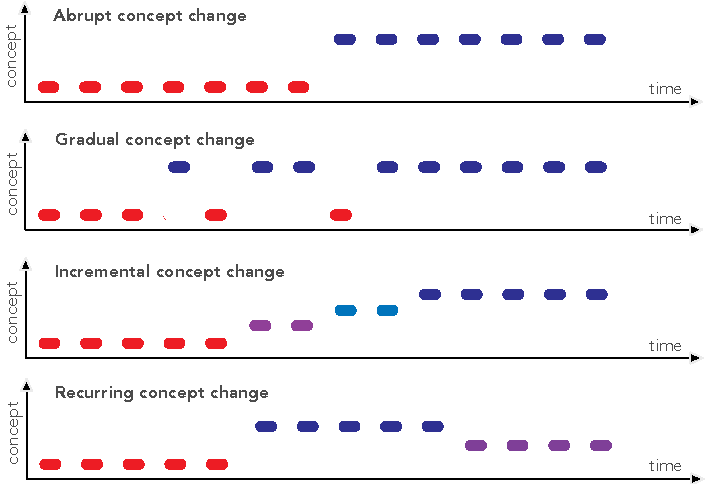
\includegraphics[width=0.7\linewidth]{files/conceptchange-9c271d1d6e6c8f363952613516aaf13c.pdf}
\caption[]{Different flavors of concept change.}
\label{fig-conceptchange}
\end{figure}

Naturally, if we acknowledge that the environment changes, it appears logical to adapt models accordingly, i.e., dynamically. This gives rise to the so-called \textbf{stability-plasticity dilemma}. This dilemma is a trade-off between model \textbf{reactiveness} (new instances have an important impact on updates) versus \textbf{stability} (these instances may not be representative of a slower trend and they may thus shift the model in a suboptimal direction).

Practically, there are two ways to shift the cursor with respect to this dilemma: alter the chronological depth of the training sample (e.g., go further back in time) or, when it's possible, allocate more weight to recent instances. For simple regressions, this idea is known as \textbf{weighted least squares} wherein errors are weighted inside the loss:

\begin{equation}
L=\sum_{i=1}^Iw_i(y_i-\textbf{x}_i\textbf{b})^2.
\end{equation}

In matrix terms, $L=(\textbf{y} -\textbf{Xb})'\textbf{W}(\textbf{y} -\textbf{Xb})$, where $\textbf{W}$ is a diagonal matrix of weights. The gradient with respect to $\textbf{b}$ is equal to $2\textbf{X}'\textbf{WX}\textbf{b} -2\textbf{X}'\textbf{Wy}$ so that the loss is minimized for $\textbf{b}^*=(\textbf{X}'\textbf{WX})^{ -1}\textbf{X}'\textbf{Wy}$. The standard least-square solution is recovered for $\textbf{W}=\textbf{I}$. In order to fine-tune the reactiveness of the model, the weights must be a function that decreases as instances become older in the sample.

There is of course no perfect solution to changing financial environments. Below, we mention two routes that are taken in the ML literature to overcome the problem of non-stationarity in the data generating process. But first, we propose yet another clear verification that markets do experience time-varying distributions.

\paragraph{Non-stationarity: yet another illustration}

One of the most basic practices in (financial) econometrics is to work with returns (relative price changes). The simple reason is that returns seem to behave consistently through time (monthly returns are bounded, they usually lie between -1 and +1). Prices on the other hand shift and, often, some prices never come back to past values. This makes prices harder to study.

Stationarity is a key notion in financial econometrics: it is much easier to characterize a phenomenon with distributional properties that remain the same through time (this makes them possible to capture). Sadly, the distribution of returns is not stationary: both the mean and the variance of returns change along cycles.

Below, we illustrate this fact by computing the average monthly return for all calendar years in the whole dataset.

\begin{figure}[!htbp]
\centering
\begin{verbatim}
# Compute average monthly return by year
data_ml['year'] = pd.to_datetime(data_ml['date']).dt.year
yearly_returns = data_ml.groupby('year')['R1M'].mean()

# Plot
fig, ax = plt.subplots(figsize=(10, 6))
yearly_returns.plot(kind='bar', ax=ax, color='steelblue', edgecolor='black')
ax.set_xlabel('Year')
ax.set_ylabel('Average Monthly Return')
ax.set_title('Average Monthly Return by Year')
ax.axhline(y=0, color='black', linestyle='-', linewidth=0.5)
plt.xticks(rotation=45)
plt.tight_layout()
plt.show()
\end{verbatim}
\caption[]{Average monthly return on a yearly basis.

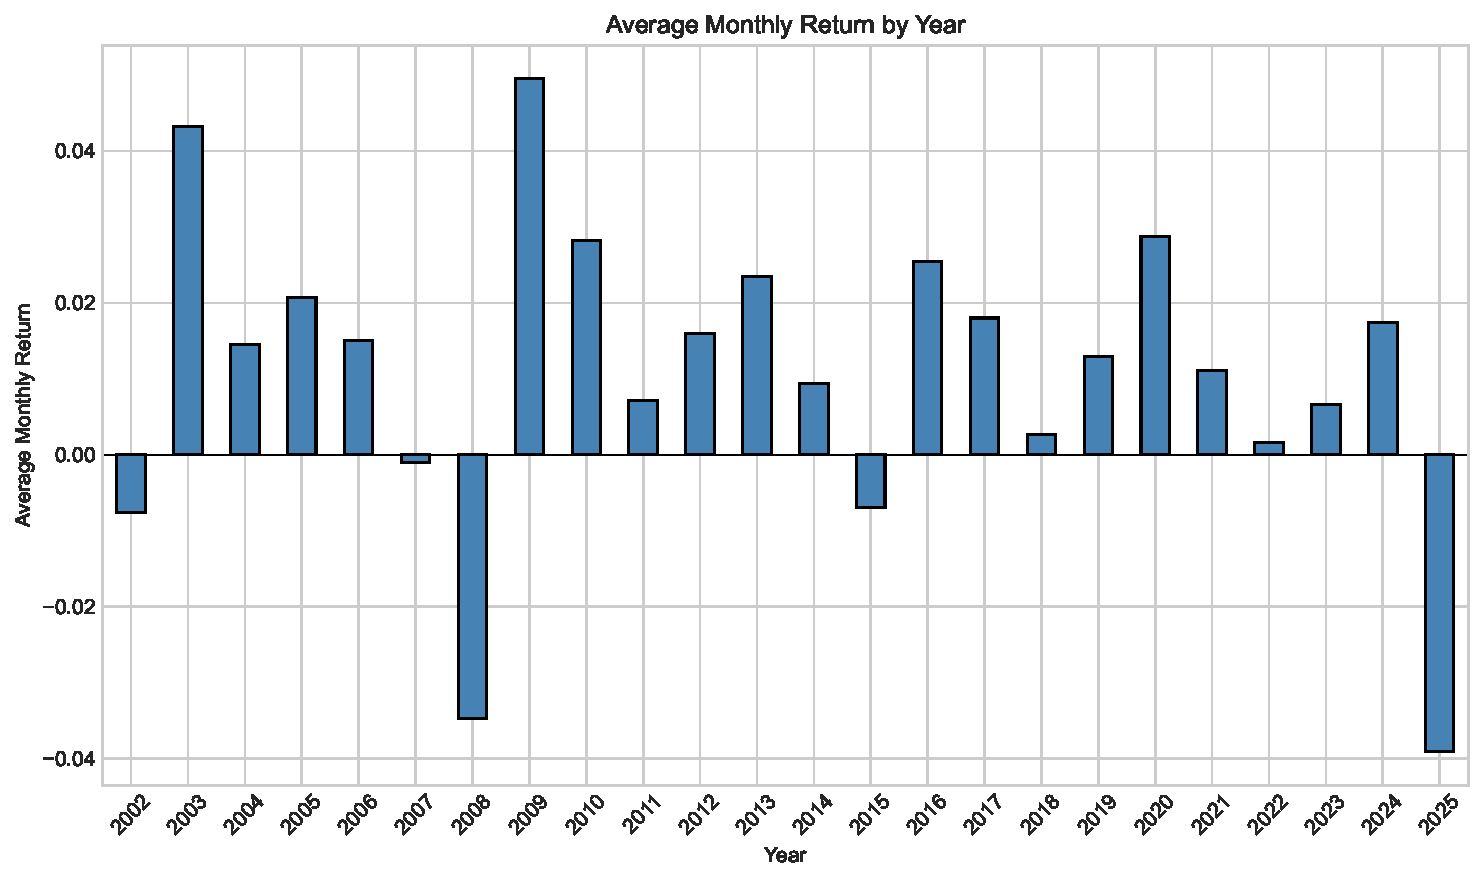
\includegraphics[width=0.7\linewidth]{files/fb00463a09b3cbdacd623709c6bc3abe.pdf}}
\label{fig-statplot}
\end{figure}

These changes in the mean are also accompanied by variations in the second moment (variance/volatility). This effect, known as volatility clustering, has been widely documented ever since the theoretical breakthrough of \cite{engle1982autoregressive} (and even well before). We refer for instance to \cite{cont2007volatility} for more details on this topic.

In terms of machine learning models, this is also true. Below, we estimate a pure characteristic regression with one predictor, the market capitalization ($r_{t+1,n}=\alpha+\beta x_{t,n}^{\text{cap}}+\epsilon_{t+1,n}$). The label is the forward return and the estimation is performed over every calendar year.

\begin{figure}[!htbp]
\centering
\begin{verbatim}
# Compute yearly beta for size_avg_252d (market cap proxy)
def get_beta(group):
    """Get regression coefficient for size_avg_252d."""
    X = sm.add_constant(group['size_avg_252d'])
    y = group['R1M']
    try:
        model = OLS(y, X).fit()
        return model.params['size_avg_252d']
    except:
        return np.nan

yearly_betas = data_ml.groupby('year').apply(get_beta)

# Plot
fig, ax = plt.subplots(figsize=(10, 6))
yearly_betas.plot(kind='bar', ax=ax, color='steelblue', edgecolor='black')
ax.set_xlabel('Year')
ax.set_ylabel('Beta (size_avg_252d)')
ax.set_title('Yearly Regression Coefficient: Returns on Market Capitalization')
ax.axhline(y=0, color='black', linestyle='-', linewidth=0.5)
plt.xticks(rotation=45)
plt.tight_layout()
plt.show()
\end{verbatim}
\caption[]{Variations in betas with respect to market capitalization.

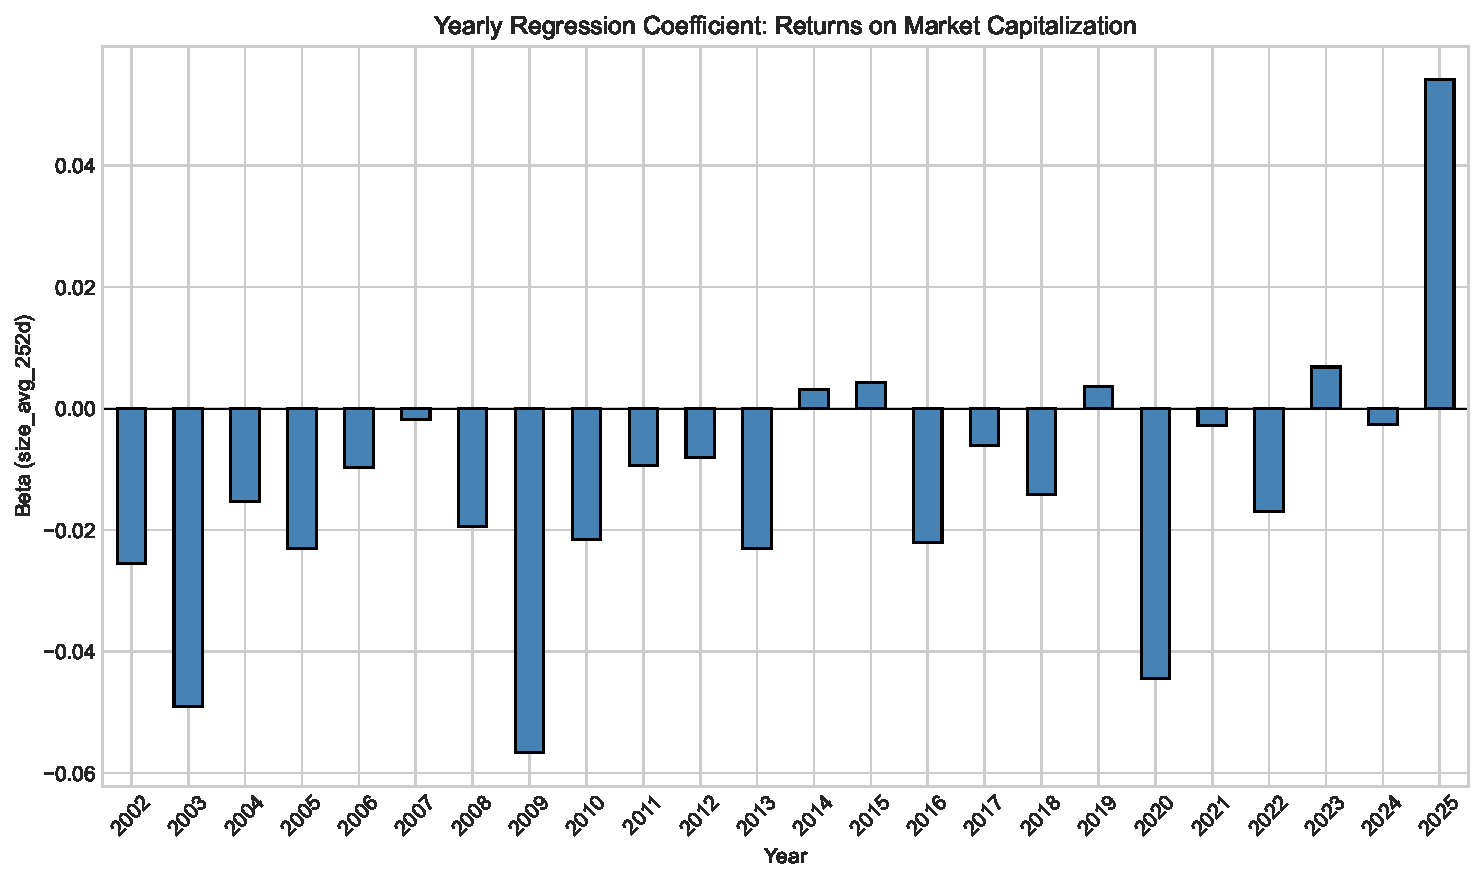
\includegraphics[width=0.7\linewidth]{files/e41365a89086e785b781e2cf9a9a4077.pdf}}
\label{fig-conceptdriftemp}
\end{figure}

\begin{verbatim}
print(f"\nMean beta: {yearly_betas.mean():.6f}")
print(f"Std of beta: {yearly_betas.std():.6f}")
print(f"Years with positive beta: {(yearly_betas > 0).sum()} / {len(yearly_betas)}")
\end{verbatim}

\begin{verbatim}
Mean beta: -0.012474
Std of beta: 0.021796
Years with positive beta: 5 / 24
\end{verbatim}

The bars in the figure highlight the concept drift: overall, the relationship between capitalization and returns may be negative (the \textbf{size effect}). Sometimes it is markedly negative, sometimes, not so much, and sometimes it even reverses. The ability of capitalization to explain returns is time-varying and models must adapt accordingly.

\paragraph{Detecting Concept Drift}

Modern machine learning provides tools to detect when concept drift occurs. Below, we implement a simple drift detection method based on monitoring prediction errors over time.

\begin{figure}[!htbp]
\centering
\begin{verbatim}
from sklearn.linear_model import LinearRegression

# Simple drift detection: monitor rolling prediction errors
def detect_drift_rolling(data, features, target, window_train=36, window_test=12):
    """
    Detect drift by monitoring rolling prediction errors.
    Train on window_train months, test on next window_test months.
    """
    # Get unique dates
    dates = sorted(data['date'].unique())
    
    results = []
    
    for i in range(window_train, len(dates) - window_test):
        train_dates = dates[i-window_train:i]
        test_dates = dates[i:i+window_test]
        
        train_data = data[data['date'].isin(train_dates)]
        test_data = data[data['date'].isin(test_dates)]
        
        if len(train_data) < 100 or len(test_data) < 50:
            continue
        
        # Train model
        X_train = train_data[features].dropna()
        y_train = train_data.loc[X_train.index, target]
        
        X_test = test_data[features].dropna()
        y_test = test_data.loc[X_test.index, target]
        
        model = LinearRegression()
        model.fit(X_train, y_train)
        
        # Compute errors
        train_mse = np.mean((y_train - model.predict(X_train))**2)
        test_mse = np.mean((y_test - model.predict(X_test))**2)
        
        results.append({
            'date': dates[i],
            'train_mse': train_mse,
            'test_mse': test_mse,
            'drift_ratio': test_mse / train_mse if train_mse > 0 else np.nan
        })
    
    return pd.DataFrame(results)

# Run drift detection
drift_results = detect_drift_rolling(
    training_sample, 
    features_short, 
    'R1M',
    window_train=24,
    window_test=6
)

# Plot drift ratio over time
fig, axes = plt.subplots(2, 1, figsize=(12, 8))

# Plot 1: MSE over time
axes[0].plot(drift_results['date'], drift_results['train_mse'], label='Train MSE', alpha=0.7)
axes[0].plot(drift_results['date'], drift_results['test_mse'], label='Test MSE', alpha=0.7)
axes[0].set_xlabel('Date')
axes[0].set_ylabel('MSE')
axes[0].set_title('Rolling Train vs Test MSE')
axes[0].legend()

# Plot 2: Drift ratio
axes[1].plot(drift_results['date'], drift_results['drift_ratio'], color='red', alpha=0.7)
axes[1].axhline(y=1, color='black', linestyle='--', label='No drift (ratio=1)')
axes[1].axhline(y=1.5, color='orange', linestyle=':', label='Warning threshold')
axes[1].set_xlabel('Date')
axes[1].set_ylabel('Test MSE / Train MSE')
axes[1].set_title('Drift Detection: Test/Train MSE Ratio')
axes[1].legend()

plt.tight_layout()
plt.show()
\end{verbatim}
\caption[]{Concept drift detection via rolling prediction errors.

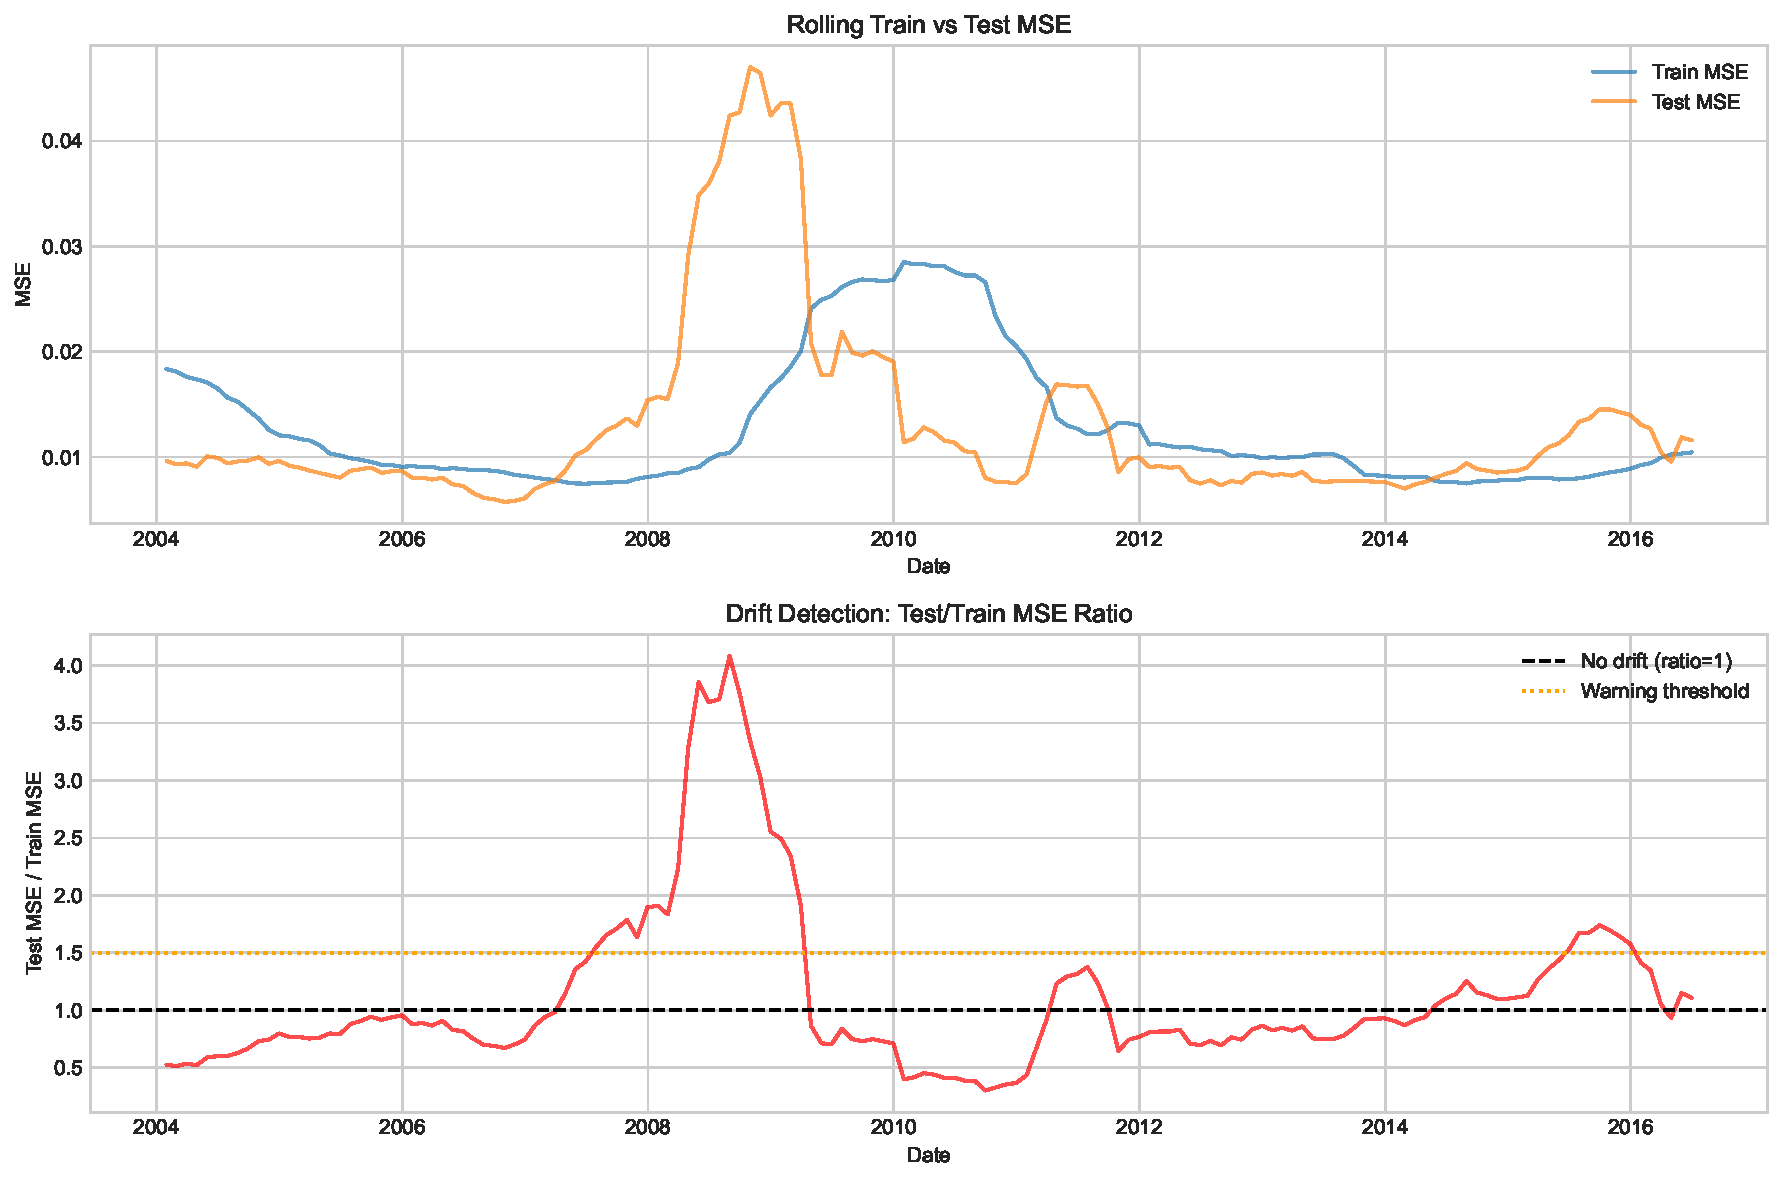
\includegraphics[width=0.7\linewidth]{files/4a9cca9857e083ade396bed4108f24a4.pdf}}
\label{fig-drift_detection}
\end{figure}

\begin{verbatim}
print(f"\nDrift Statistics:")
print(f"Mean drift ratio: {drift_results['drift_ratio'].mean():.3f}")
print(f"Max drift ratio: {drift_results['drift_ratio'].max():.3f}")
print(f"Periods with ratio > 1.5: {(drift_results['drift_ratio'] > 1.5).sum()}")
\end{verbatim}

\begin{verbatim}
Drift Statistics:
Mean drift ratio: 1.119
Max drift ratio: 4.082
Periods with ratio > 1.5: 28
\end{verbatim}

\paragraph{Online learning}

Online learning refers to a subset of machine learning in which new information arrives progressively and the integration of this flow is performed iteratively (the term `\textit{online}' is not linked to the internet). In order to take the latest data updates into account, it is imperative to update the model.

The problem is that if a 2019 model is trained on data from 2010 to 2019, the (dynamic) 2020 model will have to be re-trained with the whole dataset including the latest points from 2020. This can be heavy and including just the latest points in the learning process would substantially decrease its computational cost. In neural networks, the sequential batch updating of weights can allow a progressive change in the model.

The simplest example of online learning is the Widrow-Hoff algorithm (originally from \cite{widrow1960adaptive}). Suppose the model is linear, that is $\textbf{y}=\textbf{Xb}+\textbf{e}$ and that the amount of data is both massive and coming in at a high frequency. A simple and heuristic way to update the values of $\textbf{b}$ is to compute

\begin{equation}
\textbf{b}_{t+1} \longleftarrow \textbf{b}_t-\eta (\textbf{x}_t\textbf{b}-y_t)\textbf{x}_t',
\end{equation}

where $\textbf{x}_t$ is the row vector of instance $t$. The justification is simple. The quadratic error $(\textbf{x}_t\textbf{b} -y_t)^2$ has a gradient with respect to $\textbf{b}$ equal to $2(\textbf{x}_t\textbf{b} -y_t)\textbf{x}_t'$; therefore, the above update is a simple example of gradient descent. $\eta$ must of course be quite small: if not, each new point will considerably alter $\textbf{b}$, thereby resulting in a volatile model.

Datasets are indexed by time: we write $\textbf{X}_t$ and $\textbf{y}_t$ for features and labels. Time has a bounded horizon $T$. The machine learning model depends on some parameters $\boldsymbol{\theta}$ and we denote it with $f_{\boldsymbol{\theta}}$. At time $t$ (when dataset ($\textbf{X}_t$, $\textbf{y}_t$) is gathered), the loss function $L$ naturally depends on the data and on the model via $\boldsymbol{\theta}_t$ which are the parameter values fitted to the time-$t$ data. The key quantity in online learning is the regret over the whole time sequence:

\begin{equation}
\label{eq:regret}
R_T=\sum_{t=1}^TL_t(\boldsymbol{\theta}_t)-\underset{\boldsymbol{\theta}^*\in \boldsymbol{\Theta}}{\inf} \ \sum_{t=1}^TL_t(\boldsymbol{\theta}^*).
\end{equation}

The regret is the total loss incurred by the models $\boldsymbol{\theta}_t$ minus the minimal loss that could have been obtained with full knowledge of the data sequence (hence computed in hindsight). The basic methods in online learning are in fact quite similar to the batch-training of neural networks. The updating of the parameter is based on

\begin{equation}
\label{eq:online1}
\textbf{z}_{t+1}=\boldsymbol{\theta}_t-\eta_t\nabla L_t(\boldsymbol{\theta}_t),
\end{equation}

where $\nabla L_t(\boldsymbol{\theta}_t)$ denotes the gradient of the current loss $L_t$.

\begin{verbatim}
# Online Learning Implementation: Widrow-Hoff / LMS Algorithm

def online_sgd_regression(X, y, learning_rate=0.001, n_passes=1):
    """
    Online Stochastic Gradient Descent for linear regression.
    
    Updates weights one sample at a time.
    """
    n_samples, n_features = X.shape
    
    # Initialize weights
    weights = np.zeros(n_features)
    bias = 0
    
    # Track history
    weight_history = [weights.copy()]
    loss_history = []
    
    for _ in range(n_passes):
        for i in range(n_samples):
            # Prediction
            pred = np.dot(X[i], weights) + bias
            
            # Error
            error = pred - y[i]
            
            # Update (gradient descent step)
            weights = weights - learning_rate * error * X[i]
            bias = bias - learning_rate * error
            
            # Track
            if i % 1000 == 0:
                weight_history.append(weights.copy())
                loss_history.append(error**2)
    
    return weights, bias, weight_history, loss_history

# Prepare data for online learning
X_online = training_sample[features_short].dropna().values
y_online = training_sample.loc[training_sample[features_short].dropna().index, 'R1M'].values

# Standardize features
X_mean = X_online.mean(axis=0)
X_std = X_online.std(axis=0)
X_online_scaled = (X_online - X_mean) / (X_std + 1e-8)

# Run online learning
weights_online, bias_online, weight_hist, loss_hist = online_sgd_regression(
    X_online_scaled, y_online, learning_rate=0.0001, n_passes=3
)

print("Online SGD Results:")
print("="*50)
for i, feat in enumerate(features_short):
    print(f"{feat}: {weights_online[i]:.6f}")
print(f"Bias: {bias_online:.6f}")
\end{verbatim}

\begin{verbatim}
Online SGD Results:
==================================================
Div_yld: -0.000234
EPS: -0.002427
size_avg_252d: -0.003675
mom_252: 0.000377
OCF_Growth_1Y: 0.001241
PB: -0.001688
vol_252: 0.001514
Bias: 0.013846
\end{verbatim}

\begin{figure}[!htbp]
\centering
\begin{verbatim}
# Compare with batch OLS
from sklearn.linear_model import LinearRegression
batch_model = LinearRegression()
batch_model.fit(X_online_scaled, y_online)

# Plot weight evolution
weight_hist_arr = np.array(weight_hist)

fig, axes = plt.subplots(1, 2, figsize=(14, 5))

# Weight evolution
for i, feat in enumerate(features_short):
    axes[0].plot(weight_hist_arr[:, i], label=feat, alpha=0.7)
axes[0].set_xlabel('Update Step (x1000)')
axes[0].set_ylabel('Weight Value')
axes[0].set_title('Weight Evolution During Online Learning')
axes[0].legend(loc='best', fontsize=8)

# Compare final weights
x_pos = np.arange(len(features_short))
width = 0.35
axes[1].bar(x_pos - width/2, weights_online, width, label='Online SGD')
axes[1].bar(x_pos + width/2, batch_model.coef_, width, label='Batch OLS')
axes[1].set_xticks(x_pos)
axes[1].set_xticklabels(features_short, rotation=45, ha='right')
axes[1].set_ylabel('Coefficient Value')
axes[1].set_title('Online vs Batch Regression Coefficients')
axes[1].legend()

plt.tight_layout()
plt.show()
\end{verbatim}
\caption[]{Evolution of weights during online learning.

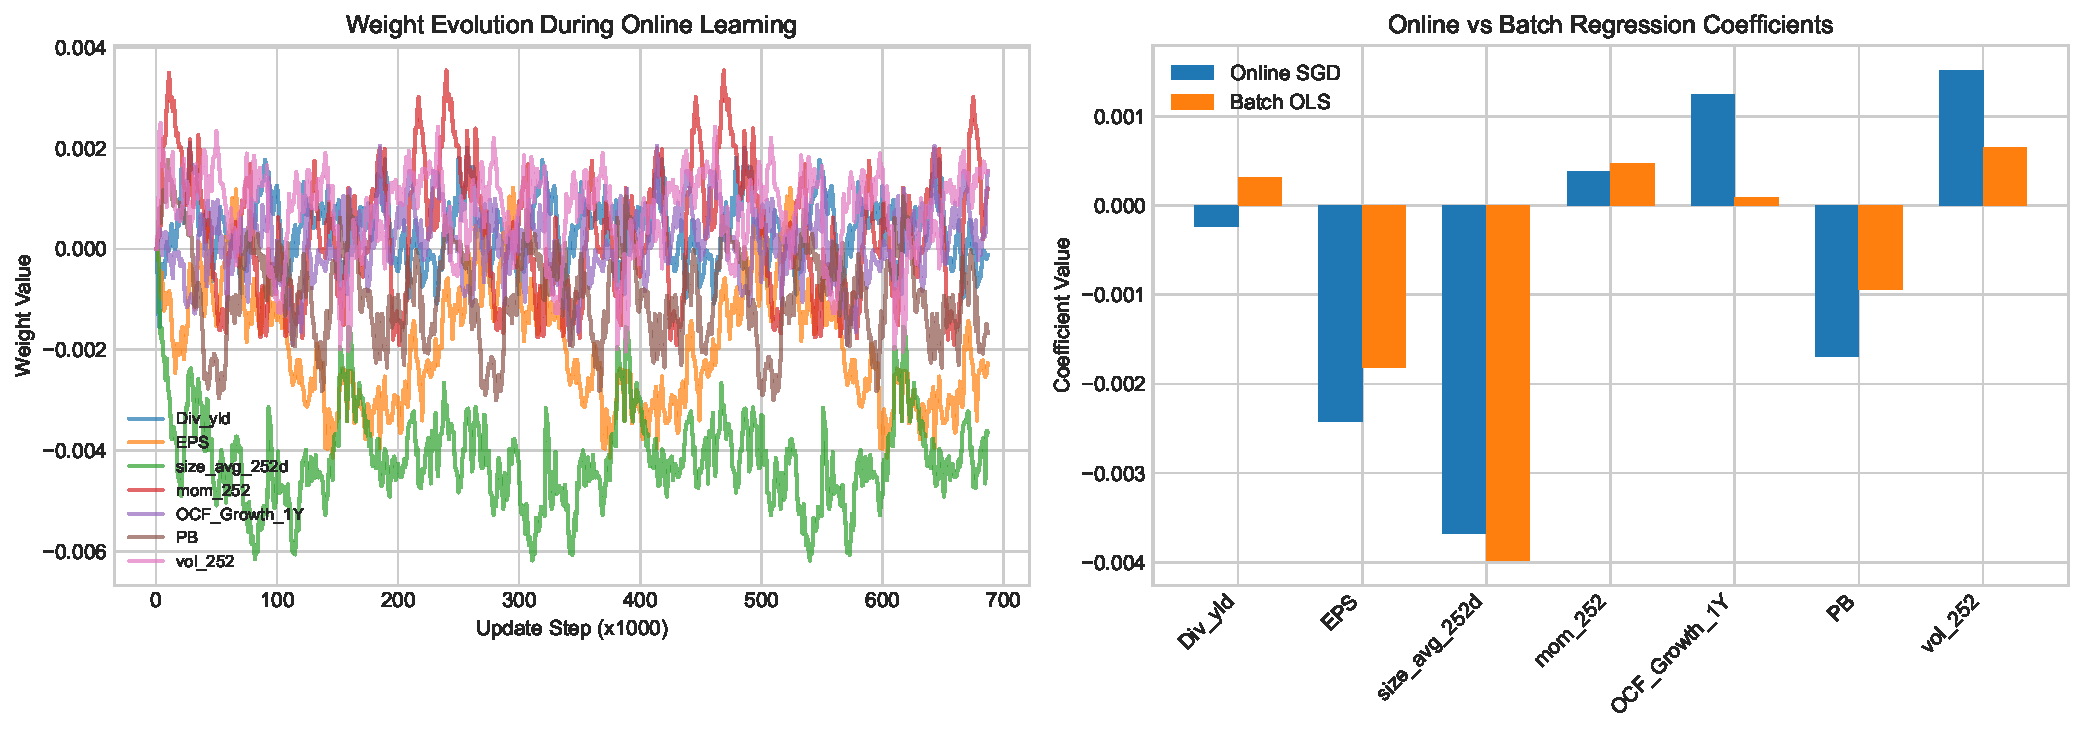
\includegraphics[width=0.7\linewidth]{files/dacf2d8718e434a29a69038283839d06.pdf}}
\label{fig-online_learning}
\end{figure}

We end this section with a historical note. Some of the ideas from online learning stem from the financial literature and from the concept of \textbf{universal portfolios} originally coined by \cite{cover1991universal} in particular. The setting is the following. The function $f$ is assumed to be linear $f(\textbf{x}_t)=\boldsymbol{\theta}'\textbf{x}_t$ and the data $\textbf{x}_t$ consists of asset returns, thus, the values are portfolio returns as long as $\boldsymbol{\theta}'\textbf{1}_N=1$ (the budget constraint). The loss functions $L_t$ correspond to a concave utility function (e.g., logarithmic) and the regret is reversed:

\begin{equation}
R_T=\underset{\boldsymbol{\theta}^*\in \boldsymbol{\Theta}}{\sup} \ \sum_{t=1}^TL_t(\textbf{r}_t'\boldsymbol{\theta}^*)-\sum_{t=1}^TL_t(\textbf{r}_t'\boldsymbol{\theta}_t),
\end{equation}

where $\textbf{r}_t'$ are the returns. Thus, the program is transformed to maximize a concave function. Several articles (often from the Computer Science or ML communities) have proposed solutions to this type of problems: \cite{blum1999universal}, \cite{agarwal2006algorithms} and \cite{hazan2007logarithmic}. The literature on online portfolio allocation is reviewed in \cite{li2014online} and outlined in more details in \cite{li2018online}.

\paragraph{Homogeneous transfer learning}

This subsection is mostly conceptual. The ideas behind transfer learning can be valuable in that they can foster novel ideas, which is why we briefly present them below.

Transfer learning has been surveyed numerous times. One classical reference is \cite{pan2009survey}, but \cite{weiss2016survey} is more recent and more exhaustive. Suppose we are given two datasets $D_S$ (source) and $D_T$ (target). Each dataset has its own features $\textbf{X}^S$ and $\textbf{X}^T$ and labels $\textbf{y}^S$ and $\textbf{y}^T$. In classical supervised learning, the patterns of the target set are learned only through $\textbf{X}^T$ and $\textbf{y}^T$. Transfer learning proposes to improve the function $f^T$ (obtained by minimizing the fit $y_i^T=f^T(\textbf{x}_i^T)+\epsilon^T_i$ on the target data) via the function $f^S$ (from $y_i^S=f^S(\textbf{x}_i^S)+\varepsilon^S_i$ on the source data). Homogeneous transfer learning is when the feature space does not change, which is the case in our setting. In asset management, this may not always be the case if for instance new predictors are included (e.g., based on alternative data like sentiment, satellite imagery, credit card logs, etc.).

There are many subcategories in transfer learning depending on what changes between the source $S$ and the target $T$: is it the feature space, the distribution of the labels, and/or the relationship between the two? The latter case is of interest in finance because the link with non-stationarity is evident: it is when the model $f$ in $\textbf{y}=f(\textbf{X})$ changes through time. In transfer learning jargon, it is written as $P[\textbf{y}^S|\textbf{X}^S]\neq P[\textbf{y}^T|\textbf{X}^T]$: the conditional law of the label knowing the features is not the same when switching from the source to the target.

An important and elegant result in the theory was proven by \cite{ben2010theory} in the case of binary classification. We consider $f$ and $h$ two classifiers with values in $\{0,1 \}$. The average error between the two over the domain $S$ is defined by

\begin{equation}
\epsilon_S(f,h)=\mathbb{E}_S[|f(\textbf{x})-h(\textbf{x})|].
\end{equation}

Then,

\begin{equation}
\epsilon_T(f_T,h)\le \epsilon_S(f_S,h)+\underbrace{2 \sup_B|P_S(B)-P_T(B)|}_{\text{ difference between domains }} + \underbrace{ \min\left(\mathbb{E}_S[|f_S(\textbf{x})-f_T(\textbf{x})|],\mathbb{E}_T[|f_S(\textbf{x})-f_T(\textbf{x})|]\right)}_{\text{difference between the two learning tasks}},
\end{equation}

where $P_S$ and $P_T$ denote the distribution of the two domains. The above inequality is a bound on the generalization performance of $h$. If we take $f_S$ to be the best possible classifier for $S$ and $f_T$ the best for $T$, then the error generated by $h$ in $T$ is smaller than the sum of three components:

\begin{itemize}
\item the error in the $S$ space;
\item the distance between the two domains (by how much the data space has shifted);
\item the distance between the two best models (generators).
\end{itemize}

One solution that is often mentioned in transfer learning is instance weighting. In machine learning, we seek to minimize

\begin{equation}
\epsilon_T(f)=\mathbb{E}_T\left[L(\text{y},f(\textbf{X})) \right],
\end{equation}

where $L$ is some loss function. This can be arranged:

\begin{equation}
\epsilon_T(f)=\mathbb{E}_S \left[\frac{P_T(\textbf{y},\textbf{X})}{P_S(\textbf{y},\textbf{X})} L(\text{y},f(\textbf{X})) \right]
\end{equation}

The key quantity is thus the transition ratio $\frac{P_T(\textbf{y},\textbf{X})}{P_S(\textbf{y},\textbf{X})}$ (Radon--Nikodym derivative under some assumptions). Of course this ratio is largely inaccessible in practice, but it is possible to find a weighting scheme (over the instances) that yields improvements over the error in the target space. The weighting scheme can be binary, thereby simply excluding some observations in the computation of the error. Simply removing observations from the training sample can have beneficial effects.

More generally, the above expression can be viewed as a theoretical invitation for user-specified instance weighting. In the asset allocation parlance, this can be viewed as introducing views as to which observations are the most interesting, e.g., value stocks can be allowed to have a larger weight in the computation of the loss if the user believes they carry more relevant information.

We close this topic by mentioning a practical application of transfer learning developed in \cite{koshiyama2020quantnet}. The authors propose a neural network architecture that allows to share the learning process from different strategies across several markets. This method is, among other things, aimed at alleviating the backtest overfitting problem.

\subsection{Unsupervised learning}

All algorithms presented in Chapters \href{/chap-06-lasso}{Penalized regressions and sparse hedging for minimum variance portfolios} to \href{/chap-11-bayes}{Bayesian methods} belong to the larger class of supervised learning tools. Such tools seek to unveil a mapping between predictors $\textbf{X}$ and a label $\textbf{Z}$. The supervision comes from the fact that it is asked that the data tries to explain this particular variable $\textbf{Z}$. Another important part of machine learning consists of unsupervised tasks, that is, when $\textbf{Z}$ is not specified and the algorithm tries to make sense of $\textbf{X}$ on its own. Often, relationships between the components of $\textbf{X}$ are identified. This field is much too vast to be summarized in one book, let alone one chapter. The purpose here is to briefly explain in what ways unsupervised learning can be used, especially in the data pre-processing phase.

\subsubsection{The problem with correlated predictors}\label{corpred}

Often, it is tempting to supply all predictors to a ML-fueled predictive engine. That may not be a good idea when some predictors are highly correlated. To illustrate this, the simplest example is a regression on two variables with zero mean and covariance and precisions matrices:

\begin{equation}
\boldsymbol{\Sigma}=\textbf{X}'\textbf{X}=\begin{bmatrix} 1 & \rho \\ \rho & 1 \end{bmatrix},  \quad \boldsymbol{\Sigma}^{-1}=\frac{1}{1-\rho^2}\begin{bmatrix} 1 & -\rho \\ -\rho & 1 \end{bmatrix}.
\end{equation}

When the covariance/correlation $\rho$ increase towards 1 (the two variables are co-linear), the scaling denominator in $\boldsymbol{\Sigma}^{ -1}$ goes to zero and the formula $\hat{\boldsymbol{\beta}}=\boldsymbol{\Sigma}^{ -1}\textbf{X}'\textbf{Z}$ implies that one coefficient will be highly positive and one highly negative. The regression creates a spurious arbitrage between the two variables. Of course, this is very inefficient and yields disastrous results out-of-sample.

We illustrate what happens when many variables are used in the regression below. One elucidation of the aforementioned phenomenon comes from the variables Mkt\_Cap\_12M and Mkt\_Cap\_6M, which have a correlation of 99.6\% in the training sample. Both are singled out as highly significant but their signs are contradictory. Moreover, the magnitude of their coefficients are very close (0.21 versus 0.18) so that their net effect cancels out. Naturally, providing the regression with only one of these two inputs would have been wiser.

\begin{verbatim}
import pandas as pd
import numpy as np
import time
import matplotlib.pyplot as plt
import seaborn as sns
import statsmodels.api as sm
from sklearn.preprocessing import StandardScaler
from sklearn.decomposition import PCA
from sklearn.cluster import KMeans
from sklearn.neighbors import NearestNeighbors
from sklearn.manifold import TSNE
from sklearn.metrics import silhouette_score
from scipy.cluster.hierarchy import dendrogram, linkage
from scipy.spatial.distance import pdist
from sklearn.ensemble import IsolationForest
import warnings
warnings.filterwarnings('ignore')

# Load data
from data_build import generate_data                                                              
data_ml, features, features_short, returns, stock_ids, stock_ids_short = generate_data()          
                                                                                                    
# Create training and testing samples                                                             
separation_date = "2017-01-15"                                                                    
training_sample = data_ml[data_ml['date'] < separation_date]                                      
testing_sample = data_ml[data_ml['date'] >= separation_date]
\end{verbatim}

\begin{verbatim}
# Regression with all features to show multicollinearity problem
X = training_sample[features].copy()
y = training_sample['R1M'].copy()

# Add constant for intercept
X_const = sm.add_constant(X)

# Fit OLS model
model = sm.OLS(y, X_const).fit()

# Get summary and filter significant predictors (|t| > 3)
results_df = pd.DataFrame({
    'term': model.params.index,
    'estimate': model.params.values,
    'std_error': model.bse.values,
    'statistic': model.tvalues.values,
    'p_value': model.pvalues.values
})

# Filter for significant predictors
significant = results_df[np.abs(results_df['statistic']) > 3].round(4)
print("Significant predictors in the training sample:")
significant
\end{verbatim}

\begin{verbatim}
Significant predictors in the training sample:
\end{verbatim}

\bigskip\noindent
\begin{tabular}{p{\dimexpr 0.167\linewidth-2\tabcolsep}p{\dimexpr 0.167\linewidth-2\tabcolsep}p{\dimexpr 0.167\linewidth-2\tabcolsep}p{\dimexpr 0.167\linewidth-2\tabcolsep}p{\dimexpr 0.167\linewidth-2\tabcolsep}p{\dimexpr 0.167\linewidth-2\tabcolsep}}
\toprule
 & term & estimate & std\_error & statistic & p\_value \\
\hline
0 & const & -0.0 & 0.0 & -1.193590e+01 & 0.0 \\
\hline
1 & Asset\_Turn & -0.0 & 0.0 & -9.180100e+00 & 0.0 \\
\hline
2 & Basic\_EPS\_Growth\_1Y & 0.0 & 0.0 & 5.429300e+00 & 0.0 \\
\hline
3 & Book\_Value\_PS & 0.0 & 0.0 & 1.067430e+01 & 0.0 \\
\hline
4 & Buyback\_Yield & -0.0 & 0.0 & -2.701570e+01 & 0.0 \\
\hline
... & ... & ... & ... & ... & ... \\
\hline
117 & vol\_22 & -0.0 & 0.0 & -2.227660e+01 & 0.0 \\
\hline
119 & vol\_66 & 0.0 & 0.0 & 3.667380e+01 & 0.0 \\
\hline
120 & Mom\_Sharp\_11M & -0.0 & 0.0 & -3.012990e+01 & 0.0 \\
\hline
121 & Mom\_Sharp\_5M & -0.0 & 0.0 & -2.813200e+01 & 0.0 \\
\hline
122 & R1M & 1.0 & 0.0 & 2.098117e+17 & 0.0 \\
\hline
\bottomrule
\end{tabular}

\bigskip

112 rows $\times$ 5 columns

In fact, there are several indicators for the market capitalization and maybe only one would suffice, but it is not obvious to tell which one is the best choice.

To further depict correlation issues, we compute the correlation matrix of the predictors below (on the training sample). Because of its dimension, we show it graphically.

\begin{verbatim}
# Correlation matrix visualization
C = training_sample[features].corr()

plt.figure(figsize=(10, 8))
sns.heatmap(C, cmap='RdBu_r', center=0, 
            xticklabels=False, yticklabels=False,
            square=True)
plt.title('Correlation matrix of predictors')
plt.tight_layout()
plt.show()
\end{verbatim}

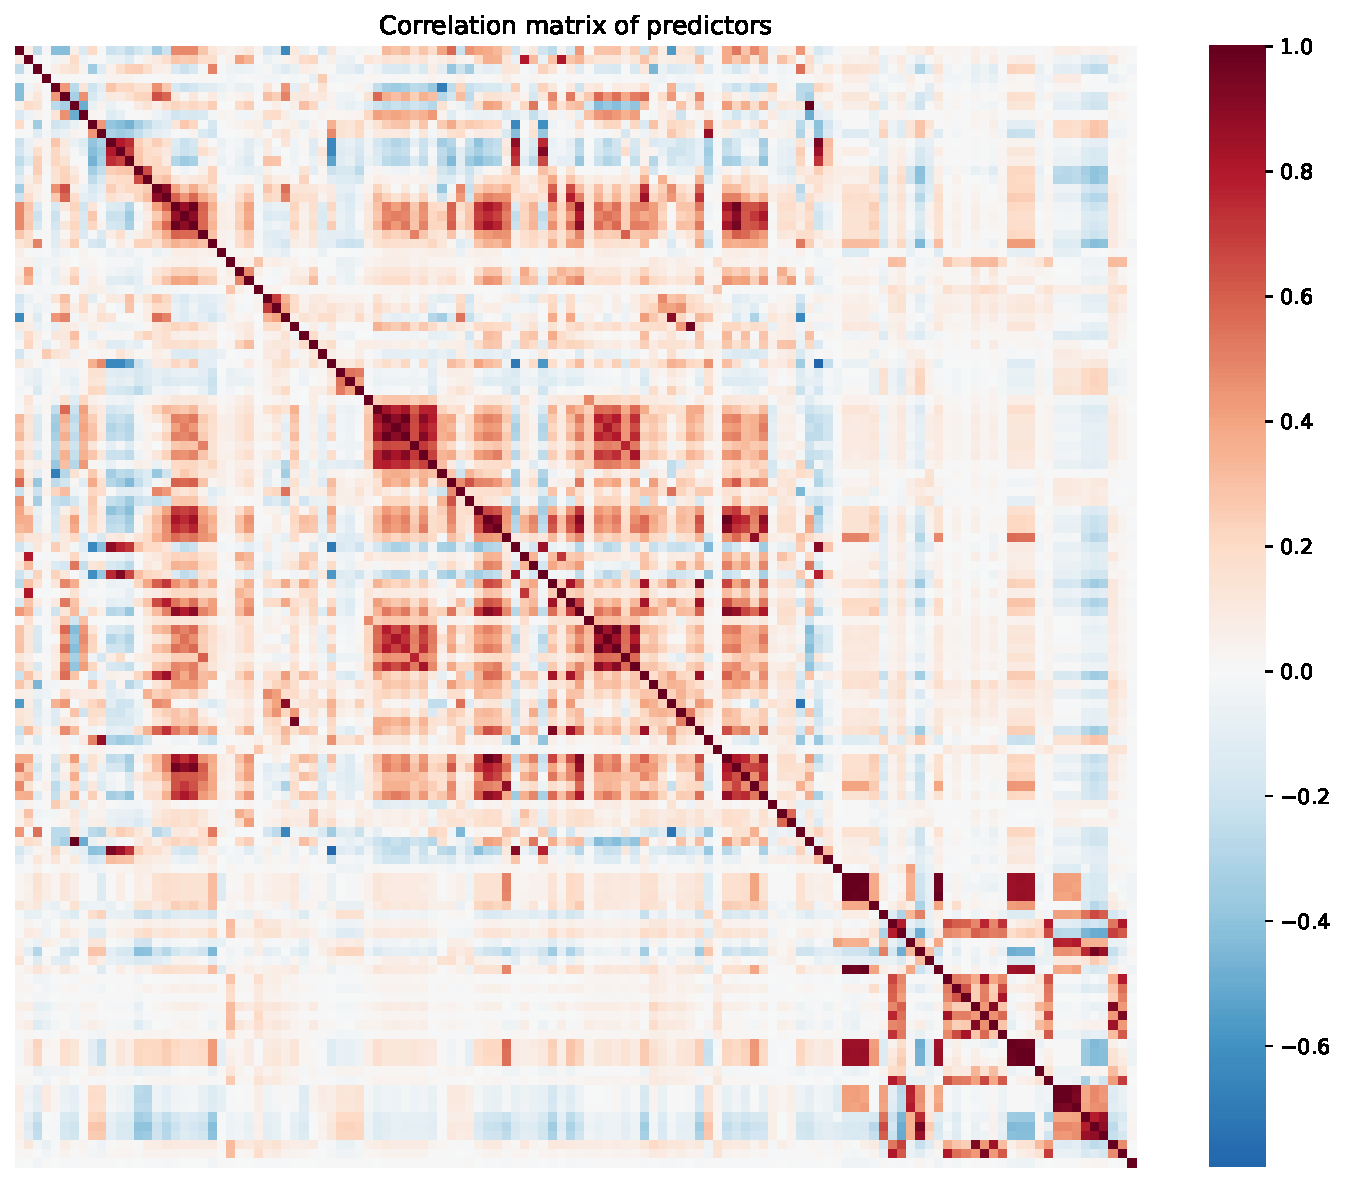
\includegraphics[width=0.7\linewidth]{files/c8b8071313cb1c9a0d37ed49b3236431.pdf}

The graph reveals several blue squares around the diagonal. For instance, the biggest square around the first third of features relates to all accounting ratios based on free cash flows. Because of this common term in their calculation, the features are naturally highly correlated. These local correlation patterns occur several times in the dataset and explain why it is not a good idea to use simple regression with this set of features.

In full disclosure, \textbf{multicollinearity} (when predictors are correlated) can be much less a problem for ML tools than it is for pure statistical inference. In statistics, one central goal is to study the properties of $\beta$ coefficients. Collinearity perturbs this kind of analysis. In machine learning, the aim is to maximize out-of-sample accuracy. If having many predictors can be helpful, then so be it. One simple example can help clarify this matter. When building a regression tree, having many predictors will give more options for the splits. If the features make sense, then they can be useful. The same reasoning applies to random forests and boosted trees. What does matter is that the large spectrum of features helps improve the generalization ability of the model. Their collinearity is irrelevant.

In the remainder of the chapter, we present two approaches that help reduce the number of predictors:

\begin{itemize}
\item the first one aims at creating new variables that are uncorrelated with each other. Low correlation is favorable from an algorithmic point of view, but the new variables lack interpretability;
\item the second one gathers predictors into homogeneous clusters and only one feature should be chosen out of this cluster. Here the rationale is reversed: interpretability is favored over statistical properties because the resulting set of features may still include high correlations, albeit to a lesser point compared to the original one.
\end{itemize}

\subsubsection{Principal component analysis and autoencoders}

The first method is a cornerstone in dimensionality reduction. It seeks to determine a smaller number of factors ($K'<K$) such that:

\begin{itemize}
\item i) the level of explanatory power remains as high as possible;
\item ii) the resulting factors are linear combinations of the original variables;
\item iii) the resulting factors are orthogonal.
\end{itemize}

\paragraph{A bit of algebra}

In this short subsection, we define some key concepts that are required to fully understand the derivation of principal component analysis (PCA). Henceforth, we work with matrices (in bold fonts). An $I \times K$ matrix $\textbf{X}$ is orthonormal if $I> K$ and $\textbf{X}'\textbf{X}=\textbf{I}_K$. When $I=K$, the (square) matrix is called orthogonal and $\textbf{X}'\textbf{X}=\textbf{X}\textbf{X}'=\textbf{I}_K$, i.e., $\textbf{X}^{ -1}=\textbf{X}'$.

One foundational result in matrix theory is the Singular Value Decomposition (SVD, see, e.g., chapter 5 in \cite{meyer2000matrix}). The SVD is formulated as follows: any $I \times K$ matrix $\textbf{X}$ can be decomposed into

\begin{equation}
\label{eq:svd}
\textbf{X}=\textbf{U} \boldsymbol{\Delta} \textbf{V}',
\end{equation}

where $\textbf{U}$ ($I\times I$) and $\textbf{V}$ ($K \times K$) are orthogonal and $\boldsymbol{\Delta}$ (with dimensions $I\times K$) is diagonal, i.e., $\Delta_{i,k}=0$ whenever $i\neq k$. In addition, $\Delta_{i,i}\ge 0$: the diagonal terms of $\boldsymbol{\Delta}$ are nonnegative.

For simplicity, we assume below that $\textbf{1}_I'\textbf{X}=\textbf{0}_K'$, i.e., that all columns have zero sum (and hence zero mean). This allows to write that the covariance matrix is equal to its sample estimate $\boldsymbol{\Sigma}_X= \frac{1}{I -1}\textbf{X}'\textbf{X}$.

One crucial feature of covariance matrices is their symmetry. Indeed, real-valued symmetric (square) matrices enjoy a SVD which is much more powerful: when $\textbf{X}$ is symmetric, there exist an orthogonal matrix $\textbf{Q}$ and a diagonal matrix $\textbf{D}$ such that

\begin{equation}
\label{eq:diagonaliz}
\textbf{X}=\textbf{Q}\textbf{DQ}'.
\end{equation}

This process is called \textbf{diagonalization} (see chapter 7 in \cite{meyer2000matrix}) and conveniently applies to covariance matrices.

\paragraph{PCA}

The goal of PCA is to build a dataset $\tilde{\textbf{X}}$ that has fewer columns but that keeps as much information as possible when compressing the original one, $\textbf{X}$. The key notion is the \textbf{change of base}, which is a linear transformation of $\textbf{X}$ into $\textbf{Z}$, a matrix with identical dimension, via

\begin{equation}
\label{eq:pca}
\textbf{Z}=\textbf{XP},
\end{equation}

where $\textbf{P}$ is a $K \times K$ matrix. There are of course an infinite number of ways to transform $\textbf{X}$ into $\textbf{Z}$, but two fundamental constraints help reduce the possibilities. The first constraint is that the columns of $\textbf{Z}$ be uncorrelated. Having uncorrelated features is desirable because they then all tell different stories and have zero redundancy. The second constraint is that the variance of the columns of $\textbf{Z}$ is highly concentrated. This means that a few factors (columns) will capture most of the explanatory power (signal), while most (the others) will consist predominantly of noise. All of this is coded in the covariance matrix of $\textbf{Z}$:

\begin{itemize}
\item the first condition imposes that the covariance matrix be diagonal;
\item the second condition imposes that the diagonal elements, when ranked in decreasing magnitude, see their value decline (sharply if possible).
\end{itemize}

The covariance matrix of $\textbf{Z}$ is

\begin{equation}
\label{eq:covy}
\boldsymbol{\Sigma}_Z=\frac{1}{I-1}\textbf{Z}'\textbf{Z}=\frac{1}{I-1}\textbf{P}'\textbf{X}'\textbf{XP}=\frac{1}{I-1}\textbf{P}'\boldsymbol{\Sigma}_X\textbf{P}.
\end{equation}

In this expression, we plug the decomposition \ref{eq:diagonaliz} of $\boldsymbol{\Sigma}_X$:
\begin{equation}
\boldsymbol{\Sigma}_Z=\frac{1}{I-1}\textbf{P}'\textbf{Q}\textbf{DQ}'\textbf{P},
\end{equation}
thus picking $\textbf{P}=\textbf{Q}$, we get, by orthogonality, $\boldsymbol{\Sigma}_Z=\frac{1}{I -1}\textbf{D}$, that is, a diagonal covariance matrix for $\textbf{Z}$. The columns of $\textbf{Z}$ can then be re-shuffled in decreasing order of variance so that the diagonal elements of $\boldsymbol{\Sigma}_Z$ progressively shrink. This is useful because it helps locate the factors with most informational content (the first factors). In the limit, a constant vector (with zero variance) carries no signal.

The matrix $\textbf{Z}$ is a linear transformation of $\textbf{X}$, thus, it is expected to carry the same information, even though this information is coded differently. Since the columns are ordered according to their relative importance, it is simple to omit some of them. The new set of features $\tilde{\textbf{X}}$ consists in the first $K'$ (with $K'<K$) columns of $\textbf{Z}$.

Below, we show how to perform PCA and visualize the output. To ease readability, we use the smaller sample with few predictors.

\begin{verbatim}
# Perform PCA on the short features
X_short = training_sample[features_short].values

# PCA with sklearn
pca = PCA()
pca.fit(X_short)

# Display results similar to R's prcomp
print("Standard deviations (singular values):")
print(np.sqrt(pca.explained_variance_))
print("\nRotation (loadings):")
loadings = pd.DataFrame(
    pca.components_.T,
    index=features_short,
    columns=[f'PC{i+1}' for i in range(len(features_short))]
)
loadings.round(4)
\end{verbatim}

\begin{verbatim}
Standard deviations (singular values):
[0.4054865  0.31204489 0.25998127 0.24991893 0.23047481 0.20274875
 0.19114423]

Rotation (loadings):
\end{verbatim}

\bigskip\noindent
\begin{tabular}{p{\dimexpr 0.125\linewidth-2\tabcolsep}p{\dimexpr 0.125\linewidth-2\tabcolsep}p{\dimexpr 0.125\linewidth-2\tabcolsep}p{\dimexpr 0.125\linewidth-2\tabcolsep}p{\dimexpr 0.125\linewidth-2\tabcolsep}p{\dimexpr 0.125\linewidth-2\tabcolsep}p{\dimexpr 0.125\linewidth-2\tabcolsep}p{\dimexpr 0.125\linewidth-2\tabcolsep}}
\toprule
 & PC1 & PC2 & PC3 & PC4 & PC5 & PC6 & PC7 \\
\hline
Div\_yld & -0.3486 & -0.3200 & 0.4117 & 0.0083 & -0.5008 & -0.2198 & 0.5545 \\
\hline
EPS & -0.5300 & -0.0022 & -0.0655 & 0.0166 & 0.7071 & -0.4250 & 0.1841 \\
\hline
size\_avg\_252d & -0.5303 & 0.0973 & -0.4247 & -0.0357 & -0.0855 & 0.6830 & 0.2322 \\
\hline
mom\_252 & -0.0189 & 0.6773 & 0.6167 & -0.2544 & 0.1487 & 0.2270 & 0.1491 \\
\hline
OCF\_Growth\_1Y & -0.0620 & 0.2199 & 0.1384 & 0.9615 & -0.0141 & 0.0611 & -0.0177 \\
\hline
PB & -0.0388 & 0.6170 & -0.4524 & -0.0508 & -0.3939 & -0.4914 & 0.1178 \\
\hline
vol\_252 & 0.5574 & -0.0193 & -0.2040 & 0.0817 & 0.2538 & 0.0885 & 0.7539 \\
\hline
\bottomrule
\end{tabular}

\bigskip

The rotation gives the matrix $\textbf{P}$: it's the tool that changes the base. The first row of the output indicates the standard deviation of each new factor (column). Each factor is indicated via a PC index (principal component). Often, the first PC (first column PC1 in the output) loads positively on all initial features: a convex weighted average of all predictors is expected to carry a lot of information. In the above example, it is almost the case, with the exception of volatility, which has a negative coefficient in the first PC. The second PC is an arbitrage between price-to-book (long) and dividend yield (short). The third PC is contrarian, as it loads heavily and negatively on momentum. Not all principal components are easy to interpret.

Sometimes, it can be useful to visualize the way the principal components are built. We show one popular representation that is used for two factors (usually the first two).

\begin{verbatim}
# PCA biplot visualization
fig, ax = plt.subplots(figsize=(8, 6))

# Scale the loadings by explained variance ratio for visualization
scale = np.sqrt(pca.explained_variance_ratio_[:2]) * 5

# Plot arrows for each feature
for i, feature in enumerate(features_short):
    ax.arrow(0, 0, 
             pca.components_[0, i] * scale[0], 
             pca.components_[1, i] * scale[1],
             head_width=0.03, head_length=0.02, fc='steelblue', ec='steelblue')
    ax.text(pca.components_[0, i] * scale[0] * 1.1, 
            pca.components_[1, i] * scale[1] * 1.1,
            feature, fontsize=10, ha='center')

# Formatting
ax.set_xlim(-1, 1)
ax.set_ylim(-1, 1)
ax.set_xlabel(f'PC1 ({pca.explained_variance_ratio_[0]*100:.1f}%)')
ax.set_ylabel(f'PC2 ({pca.explained_variance_ratio_[1]*100:.1f}%)')
ax.set_title('Visual representation of PCA with two dimensions')
ax.axhline(y=0, color='gray', linestyle='--', linewidth=0.5)
ax.axvline(x=0, color='gray', linestyle='--', linewidth=0.5)
ax.set_aspect('equal')
plt.tight_layout()
plt.show()
\end{verbatim}

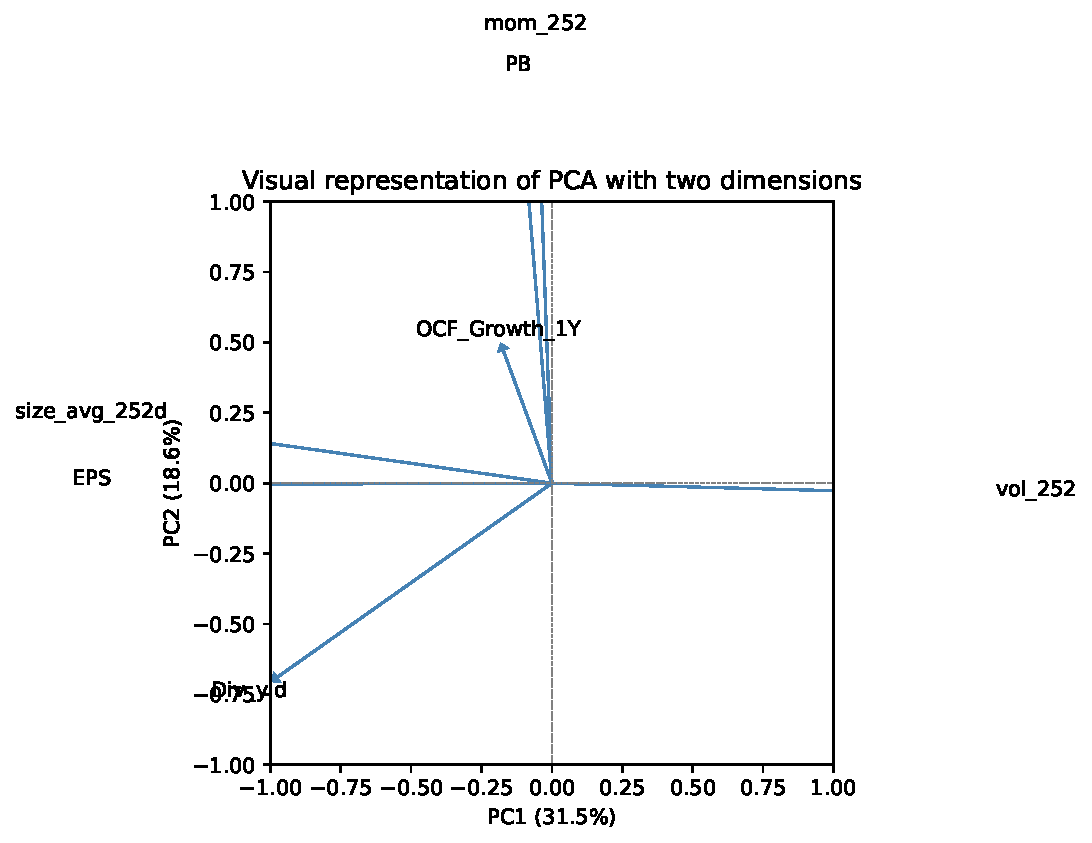
\includegraphics[width=0.7\linewidth]{files/7bc5219b84164419d76f108fb1a69720.pdf}

The plot shows the direction and magnitude of each feature's contribution to the first two principal components. The numbers indicated along the axes are the proportion of explained variance of each PC.

Once the rotation is known, it is possible to select a subsample of the transformed data. From the original 7 features, it is easy to pick just 4.

\begin{verbatim}
# Transform data using first 4 principal components
X_transformed = training_sample[features_short].values @ pca.components_.T[:, :4]

# Create DataFrame with transformed data
pca_df = pd.DataFrame(
    X_transformed,
    columns=['PC1', 'PC2', 'PC3', 'PC4']
)
pca_df.head(6)
\end{verbatim}

\bigskip\noindent
\begin{tabular}{p{\dimexpr 0.200\linewidth-2\tabcolsep}p{\dimexpr 0.200\linewidth-2\tabcolsep}p{\dimexpr 0.200\linewidth-2\tabcolsep}p{\dimexpr 0.200\linewidth-2\tabcolsep}p{\dimexpr 0.200\linewidth-2\tabcolsep}}
\toprule
 & PC1 & PC2 & PC3 & PC4 \\
\hline
0 & -0.098630 & 0.751894 & -0.106732 & 0.352415 \\
\hline
1 & -0.098418 & 0.752089 & -0.106983 & 0.352410 \\
\hline
2 & -0.098323 & 0.752172 & -0.107090 & 0.352408 \\
\hline
3 & -0.097859 & 0.752573 & -0.107602 & 0.352397 \\
\hline
4 & -0.098096 & 0.752353 & -0.107319 & 0.352402 \\
\hline
5 & -0.098096 & 0.752353 & -0.107319 & 0.352402 \\
\hline
\bottomrule
\end{tabular}

\bigskip

These 4 factors can then be used as orthogonal features in any ML engine. The fact that the features are uncorrelated is undoubtedly an asset. But the price of this convenience is high: the features are no longer immediately interpretable. De-correlating the predictors adds yet another layer of ``\textit{blackbox-ing}'' in the algorithm.

PCA can also be used to estimate factor models. In Equation \ref{eq:pca}, it suffices to replace $\textbf{Z}$ with returns, $\textbf{X}$ with factor values and $\textbf{P}$ with factor loadings (see, e.g., \cite{connor1988risk} for an early reference). More recently, \cite{lettau2018estimating} and \cite{lettau2018factors} propose a thorough analysis of PCA estimation techniques. They notably argue that first moments of returns are important and should be included in the objective function, alongside the optimization on the second moments.

We end this subsection with a technical note. Usually, PCA is performed on the covariance matrix of returns. Sometimes, it may be preferable to decompose the \textbf{correlation} matrix. The result may adjust substantially if the variables have very different variances (which is not really the case in the equity space). If the investment universe encompasses several asset classes, then a correlation-based PCA will reduce the importance of the most volatile class. In this case, it is as if all returns are scaled by their respective volatilities.

\paragraph{Scree plot and explained variance}

A useful diagnostic for PCA is the scree plot, which shows the proportion of variance explained by each principal component. This helps determine how many components to retain.

\begin{verbatim}
# Scree plot
fig, axes = plt.subplots(1, 2, figsize=(12, 4))

# Individual explained variance
axes[0].bar(range(1, len(pca.explained_variance_ratio_) + 1), 
            pca.explained_variance_ratio_, color='steelblue')
axes[0].set_xlabel('Principal Component')
axes[0].set_ylabel('Variance Explained')
axes[0].set_title('Scree Plot')
axes[0].set_xticks(range(1, len(pca.explained_variance_ratio_) + 1))

# Cumulative explained variance
cumulative_var = np.cumsum(pca.explained_variance_ratio_)
axes[1].plot(range(1, len(cumulative_var) + 1), cumulative_var, 'o-', color='steelblue')
axes[1].axhline(y=0.9, color='red', linestyle='--', label='90% threshold')
axes[1].set_xlabel('Number of Components')
axes[1].set_ylabel('Cumulative Variance Explained')
axes[1].set_title('Cumulative Explained Variance')
axes[1].set_xticks(range(1, len(cumulative_var) + 1))
axes[1].legend()

plt.tight_layout()
plt.show()

print(f"\nVariance explained by first 4 components: {cumulative_var[3]*100:.1f}%")
\end{verbatim}

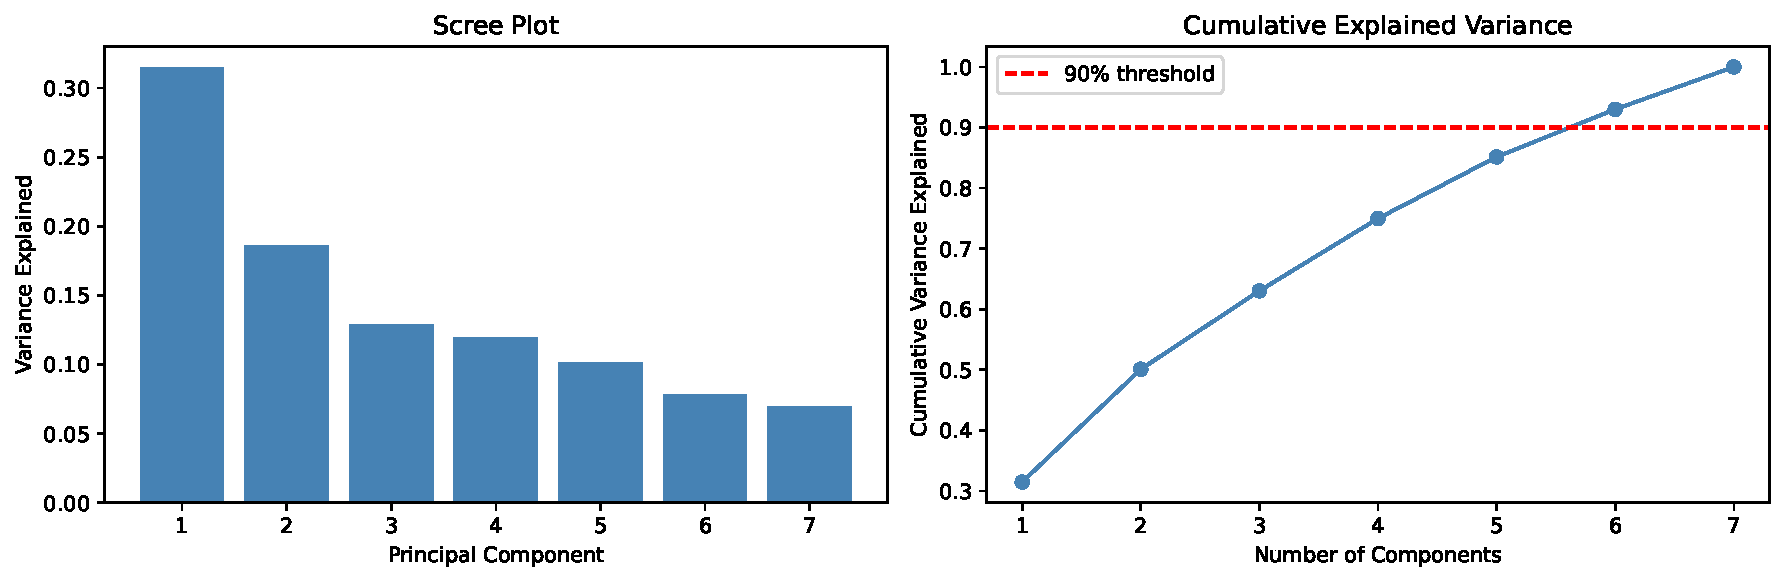
\includegraphics[width=0.7\linewidth]{files/08094cd3ae92cd30057e33e45e0dbedd.pdf}

\begin{verbatim}
Variance explained by first 4 components: 75.0%
\end{verbatim}

\paragraph{Autoencoders}\label{ae}

In a PCA, the coding from $\textbf{X}$ to $\textbf{Z}$ is straightfoward, linear and works both ways:
\begin{equation}
\textbf{Z}=\textbf{X}\textbf{P} \quad \text{and} \quad \textbf{X}=\textbf{ZP}',
\end{equation}
so that we recover $\textbf{X}$ from $\textbf{Z}$. This can be writen differently:

\begin{equation}
\label{eq:pcascheme}
\textbf{X} \quad \overset{\text{encode via }\textbf{P}}{\longrightarrow} \quad \textbf{Z} \quad \overset{\text{decode via } \textbf{P}'}{\longrightarrow} \quad \textbf{X}
\end{equation}

If we take the truncated version and seek a smaller output (with only $K'$ columns), this gives:

\begin{equation}
\label{eq:pcaschem2}
\textbf{X}, \ (I\times K) \quad \overset{\text{encode via }\textbf{P}_{K'}}{\longrightarrow} \quad \tilde{\textbf{X}}, \ (I \times K') \quad \overset{\text{decode via } \textbf{P}'_{K'}}{\longrightarrow} \quad \breve{\textbf{X}},\ (I \times K),
\end{equation}

where $\textbf{P}_{K'}$ is the restriction of $\textbf{P}$ to the $K'$ columns that correspond to the factors with the largest variances. The dimensions of matrices are indicated inside the brackets. In this case, the recoding cannot recover $\textbf{X}$ exactly but only an approximation, which we write $\breve{\textbf{X}}$. This approximation is coded with less information, hence this new data $\breve{\textbf{X}}$ is compressed and provides a parsimonious representation of the original sample $\textbf{X}$.

An autoencodeur generalizes this concept to \textbf{nonlinear} coding functions. Simple linear autoencoders are linked to latent factor models (see Proposition 1 in \cite{gu2019autoencoder} for the case of single layer autoencoders.) The scheme is the following

\begin{equation}
\label{eq:aescheme2}
\textbf{X},\ (I\times K) \quad \overset{\text{encode via } N} {\longrightarrow} \quad \tilde{\textbf{X}}=N(\textbf{X}), \ (I \times K') \quad \overset{\text{decode via } N'}{\longrightarrow} \quad \breve{\textbf{X}}=N'(\tilde{\textbf{X}}), \ (I \times K),
\end{equation}

where the encoding and decoding functions $N$ and $N'$ are often taken to be neural networks. The term \textbf{autoencoder} comes from the fact that the target output, which we often write $\textbf{Z}$ is the original sample $\textbf{X}$. Thus, the algorithm seeks to determine the function $N$ that minimizes the distance (to be defined) between $\textbf{X}$ and the output value $\breve{\textbf{X}}$. The encoder generates an alternative representation of $\textbf{X}$, whereas the decoder tries to recode it back to its original values. Naturally, the intermediate (coded) version $\tilde{\textbf{X}}$ is targeted to have a smaller dimension compared to $\textbf{X}$.

\paragraph{Application}

Autoencoders are easy to code in Keras (see Chapter \href{/chap-08-neural-networks}{Neural networks} for more details on Keras). We use the functional API. For simplicity, we work with the small number of predictors (7). The structure of the network consists of two symmetric networks with only one intermediate layer containing 32 units. The activation function is sigmoid; this makes sense since the input has values in the unit interval.

\begin{verbatim}
import os                                                                                         
os.environ["KERAS_BACKEND"] = "jax"                                                                                                                                                                   
import keras                                                                                      
from keras import layers, Model 
import keras.ops as ops  

# Set random seed for reproducibility
import jax                                                                                        
key = jax.random.PRNGKey(42)   

# Define the autoencoder architecture
input_layer = keras.Input(shape=(7,))  # features_short has 7 columns

# Encoder
encoded = layers.Dense(32, activation='sigmoid')(input_layer)
encoded = layers.Dense(4)(encoded)  # 4 dimensions for the output layer (same as PCA example)

# Decoder
decoded = layers.Dense(32, activation='sigmoid')(encoded)
decoded = layers.Dense(7)(decoded)  # the original sample has 7 features

# Build the autoencoder model
ae_model = Model(inputs=input_layer, outputs=decoded)

# Compile with MSE loss and Adam optimizer
ae_model.compile(
    optimizer='adam',
    loss='mean_squared_error',
    metrics=['mean_absolute_error']
)

ae_model.summary()
\end{verbatim}

\begin{verbatim}
Model: "functional"
\end{verbatim}

\begin{verbatim}
+---------------------------------+------------------------+---------------+
| Layer (type)                    | Output Shape           |       Param # |
+---------------------------------+------------------------+---------------+
| input_layer (InputLayer)        | (None, 7)              |             0 |
+---------------------------------+------------------------+---------------+
| dense (Dense)                   | (None, 32)             |           256 |
+---------------------------------+------------------------+---------------+
| dense_1 (Dense)                 | (None, 4)              |           132 |
+---------------------------------+------------------------+---------------+
| dense_2 (Dense)                 | (None, 32)             |           160 |
+---------------------------------+------------------------+---------------+
| dense_3 (Dense)                 | (None, 7)              |           231 |
+---------------------------------+------------------------+---------------+
\end{verbatim}

\begin{verbatim}
Total params: 779 (3.04 KB)
\end{verbatim}

\begin{verbatim}
Trainable params: 779 (3.04 KB)
\end{verbatim}

\begin{verbatim}
Non -trainable params: 0 (0.00 B)
\end{verbatim}

In the training part, we optimize the MSE and use an Adam update of the weights (see Section~\ref{backprop}). The evolution of loss on the training and testing samples is depicted below. The decreasing pattern shows the progress of the quality in compression.

\begin{verbatim}
# Prepare data
X_train = training_sample[features_short].values
X_test = testing_sample[features_short].values

# Train the autoencoder
history = ae_model.fit(                                                                           
      X_train, X_train,  # Input and target are the same for autoencoders                           
      epochs=15,                                                                                    
      batch_size=512,                                                                               
      validation_data=(X_test, X_test),                                                             
      verbose=1                                                                                     
  )
\end{verbatim}

\begin{verbatim}
447/447 -------------------- 0s 891us/step - loss: 0.0187 - mean_absolute_error: 0.0984 - val_loss: 0.0175 - val_mean_absolute_error: 0.0953
\end{verbatim}

\begin{verbatim}
# Plot training history
fig, axes = plt.subplots(1, 2, figsize=(12, 4))

# Loss
axes[0].plot(history.history['loss'], label='Training')
axes[0].plot(history.history['val_loss'], label='Validation')
axes[0].set_xlabel('Epoch')
axes[0].set_ylabel('Loss (MSE)')
axes[0].set_title('Output from the training of an autoencoder')
axes[0].legend()

# MAE
axes[1].plot(history.history['mean_absolute_error'], label='Training')
axes[1].plot(history.history['val_mean_absolute_error'], label='Validation')
axes[1].set_xlabel('Epoch')
axes[1].set_ylabel('Mean Absolute Error')
axes[1].set_title('MAE over epochs')
axes[1].legend()

plt.tight_layout()
plt.show()
\end{verbatim}

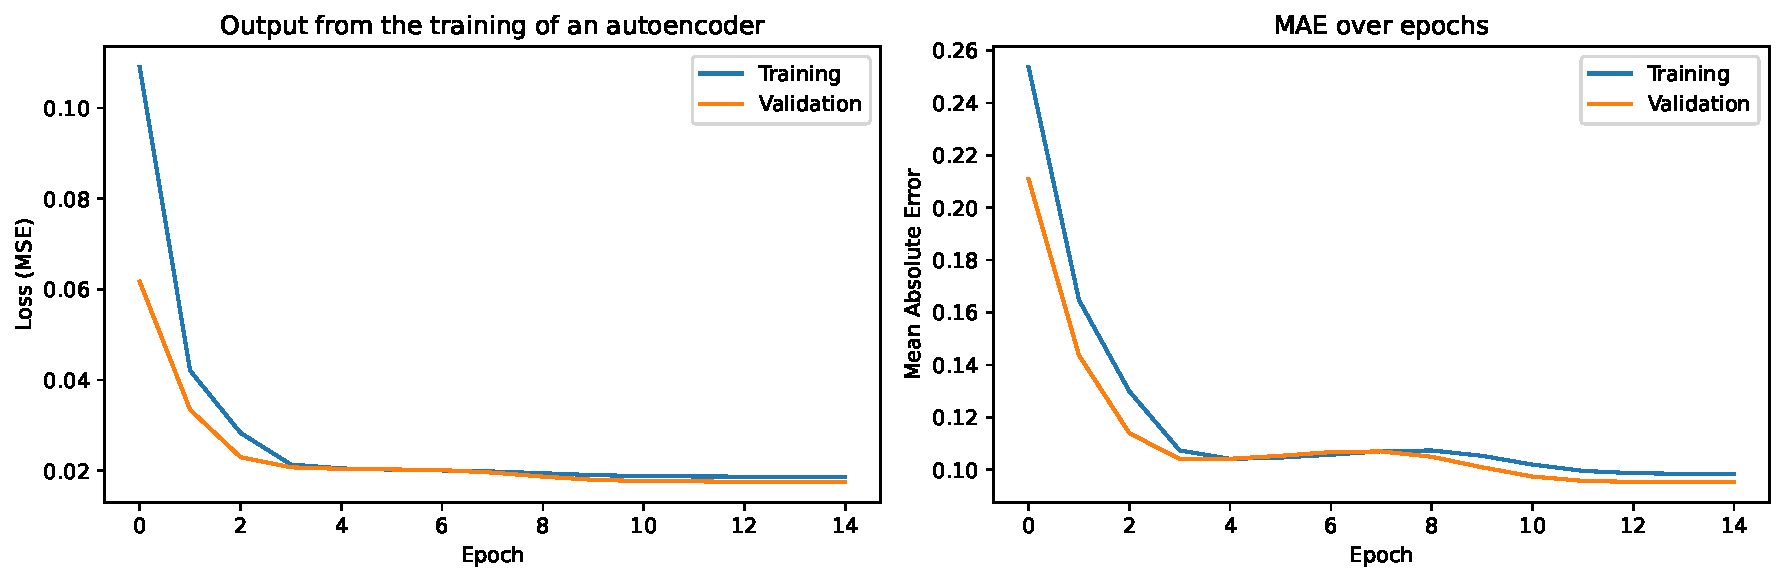
\includegraphics[width=0.7\linewidth]{files/154286307a914e87e74792ecd519c7ff.pdf}

In order to get the details of all weights and biases, the syntax is the following.

\begin{verbatim}
# Get weights
ae_weights = ae_model.get_weights()
print(f"Number of weight arrays: {len(ae_weights)}")
for i, w in enumerate(ae_weights):
    print(f"Layer {i}: shape = {w.shape}")
\end{verbatim}

\begin{verbatim}
Number of weight arrays: 8
Layer 0: shape = (7, 32)
Layer 1: shape = (32,)
Layer 2: shape = (32, 4)
Layer 3: shape = (4,)
Layer 4: shape = (4, 32)
Layer 5: shape = (32,)
Layer 6: shape = (32, 7)
Layer 7: shape = (7,)
\end{verbatim}

Retrieving the encoder and processing the data into the compressed format is just a matter of extracting the encoder part of the model.

\begin{verbatim}
# Build encoder model (extracts the compressed representation)
encoder_model = Model(inputs=input_layer, outputs=encoded)

# Get compressed representation of training data
X_compressed = encoder_model.predict(X_train[:6])
pd.DataFrame(X_compressed, columns=['AE1', 'AE2', 'AE3', 'AE4'])
\end{verbatim}

\begin{verbatim}
1/1 -------------------- 0s 26ms/step
\end{verbatim}

\bigskip\noindent
\begin{tabular}{p{\dimexpr 0.200\linewidth-2\tabcolsep}p{\dimexpr 0.200\linewidth-2\tabcolsep}p{\dimexpr 0.200\linewidth-2\tabcolsep}p{\dimexpr 0.200\linewidth-2\tabcolsep}p{\dimexpr 0.200\linewidth-2\tabcolsep}}
\toprule
 & AE1 & AE2 & AE3 & AE4 \\
\hline
0 & 0.028365 & 0.244199 & -0.137838 & -0.421712 \\
\hline
1 & 0.028082 & 0.244639 & -0.137827 & -0.421636 \\
\hline
2 & 0.027962 & 0.244831 & -0.137824 & -0.421603 \\
\hline
3 & 0.027390 & 0.245763 & -0.137814 & -0.421444 \\
\hline
4 & 0.027711 & 0.245270 & -0.137827 & -0.421528 \\
\hline
5 & 0.027711 & 0.245270 & -0.137827 & -0.421528 \\
\hline
\bottomrule
\end{tabular}

\bigskip

\paragraph{Variational Autoencoders (VAE)}

A more advanced variant is the \textbf{Variational Autoencoder} (VAE), which learns a probabilistic latent space. Instead of encoding inputs to fixed points, VAEs encode inputs to distributions, enabling smooth interpolation and generation of new samples. VAEs are particularly useful when you want to generate new synthetic data that resembles your training data.

\subsubsection{Visualization via t-SNE}

While PCA is excellent for linear dimensionality reduction, non-linear methods like \textbf{t-SNE} (t-distributed Stochastic Neighbor Embedding) and \textbf{UMAP} (Uniform Manifold Approximation and Projection) are powerful for visualizing high-dimensional data in 2D or 3D. These methods preserve local structure better than PCA, making them ideal for discovering clusters and patterns.

Note that these methods are primarily for \textbf{visualization}, not for creating features to use in downstream models, as they don't provide a transformation that can be applied to new data out-of-the-box.

\begin{verbatim}
# Take a subsample for faster computation
np.random.seed(42)
sample_idx = np.random.choice(len(X_train), size=5000, replace=False)
X_sample = X_train[sample_idx]

# Apply t-SNE
tsne = TSNE(n_components=2, perplexity=30, random_state=42)
X_tsne = tsne.fit_transform(X_sample)

# Plot
plt.figure(figsize=(8, 6))
plt.scatter(X_tsne[:, 0], X_tsne[:, 1], alpha=0.5, s=10, c='steelblue')
plt.xlabel('t-SNE 1')
plt.ylabel('t-SNE 2')
plt.title('t-SNE visualization of feature space')
plt.tight_layout()
plt.show()
\end{verbatim}

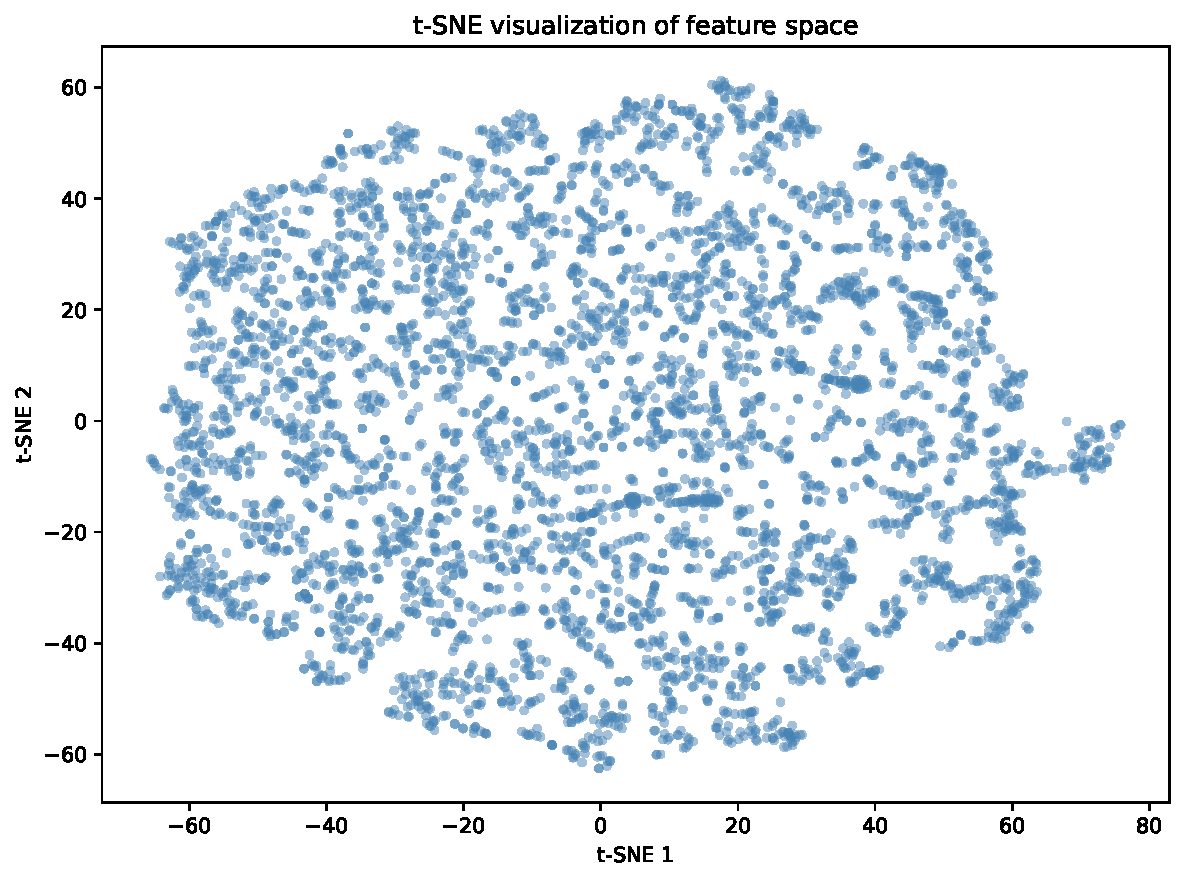
\includegraphics[width=0.7\linewidth]{files/d402c6e3b6ae46502612b3cde9ca3803.pdf}

\subsubsection{Clustering via k-means}

The second family of unsupervised tools pertains to clustering. Features are grouped into homogeneous families of predictors. It is then possible to single out one among the group (or to create a synthetic average of all of them). Mechanically, the number of predictors is reduced.

The principle is simple: among a group of variables (the reasoning would be the same for observations in the other dimension) $\textbf{x}_{\{1 \le j \le J\}}$, find the combination of $k<J$ groups that minimize

\begin{equation}
\label{eq:kmeans}
\sum_{i=1}^k\sum_{\textbf{x}\in S_i}||\textbf{x}-\textbf{m}_i||^2,
\end{equation}

where $||\cdot ||$ is some norm which is usually taken to be the Euclidean $l^2$-norm. The $S_i$ are the groups and the minimization is run on the whole set of groups $\textbf{S}$. The $\textbf{m}_i$ are the group means (also called centroids or barycenters): $\textbf{m}_i=(\text{card}(S_i))^{ -1}\sum_{\textbf{x}\in S_i}\textbf{x}$.

In order to ensure optimality, all possible arrangements must be tested, which is prohibitively long when $k$ and $J$ are large. Therefore, the problem is usually solved with greedy algorithms that seek (and find) solutions that are not optimal but `good enough'.

One heuristic way to proceed is the following:

\begin{enumerate}[resume]
\item Start with a (possibly random) partition of $k$ clusters.
\item For each cluster, compute the optimal mean values $\textbf{m}_i^*$ that minimizes expression \ref{eq:kmeans}. This is a simple quadratic program.
\item Given the optimal centers $\textbf{m}_i^*$, reassign the points $\textbf{x}_i$ so that they are all the closest to their center.
\item Repeat steps 1. and 2. until the points do not change cluster at step 2.
\end{enumerate}

Below, we illustrate this process with an example. From all 93 features, we build 10 clusters.

\begin{verbatim}
# K-means clustering of features (transpose to cluster columns)
np.random.seed(42)

# Get feature matrix and transpose to cluster features (columns)
X_features = training_sample[features].values.T  # Shape: (n_features, n_samples)

# Perform k-means clustering
kmeans = KMeans(n_clusters=6, random_state=42, n_init=6)
feature_clusters = kmeans.fit_predict(X_features)

# Organize clusters
clusters_df = pd.DataFrame({
    'factor': features,
    'cluster': feature_clusters
}).sort_values('cluster')

# Show one particular group (cluster 2)
print("Members of cluster 2:")
clusters_df[clusters_df['cluster'] == 2]
\end{verbatim}

\begin{verbatim}
Members of cluster 2:
\end{verbatim}

\bigskip\noindent
\begin{tabular}{p{\dimexpr 0.333\linewidth-2\tabcolsep}p{\dimexpr 0.333\linewidth-2\tabcolsep}p{\dimexpr 0.333\linewidth-2\tabcolsep}}
\toprule
 & factor & cluster \\
\hline
91 & adv\_252 & 2 \\
\hline
110 & size\_log & 2 \\
\hline
109 & size\_avg\_66d & 2 \\
\hline
100 & log\_adv\_21 & 2 \\
\hline
108 & size\_avg\_252d & 2 \\
\hline
93 & bb\_width & 2 \\
\hline
92 & adv\_63 & 2 \\
\hline
90 & adv\_180 & 2 \\
\hline
\bottomrule
\end{tabular}

\bigskip

We single out the fourth cluster which is composed mainly of accounting ratios. Given these 10 clusters, we can build a much smaller group of features that can then be fed to the predictive engines described in Chapters \href{/chap-06-lasso}{Penalized regressions and sparse hedging for minimum variance portfolios} to \href{/chap-11-bayes}{Bayesian methods}. The representative of a cluster can be the member that is closest to the center, or simply the center itself. This pre-processing step can nonetheless cause problems in the forecasting phase. Typically, it requires that the training data be also clustered. The extension to the testing data is not straightforward (the clusters may not be the same).

\begin{verbatim}
# Show all clusters
for i in range(6):
    cluster_members = clusters_df[clusters_df['cluster'] == i]['factor'].tolist()
    print(f"\nCluster {i} ({len(cluster_members)} members):")
    print(", ".join(cluster_members[:5]), end="")
    if len(cluster_members) > 5:
        print(f", ... (+{len(cluster_members)-5} more)")
    else:
        print()
\end{verbatim}

\begin{verbatim}
Cluster 0 (16 members):
Mom_Sharp_5M, dd, EPS_Quarterly_Surprise, ma_ratio, macd, ... (+11 more)

Cluster 1 (15 members):
Pretax_Income_Margin, PSales, PE, Gross_Margin, Net_Profit_Margin, ... (+10 more)

Cluster 2 (8 members):
adv_252, size_log, size_avg_66d, log_adv_21, size_avg_252d, ... (+3 more)

Cluster 3 (55 members):
ROIC, Normalized_ROA, OCF_Growth_1Y, OCF_to_Assets, OCF_to_NOA, ... (+50 more)

Cluster 4 (14 members):
Debt_equity, Debt_Assets, Div_yld, Capex_Intensity, Buyback_Yield, ... (+9 more)

Cluster 5 (14 members):
vol_66, vol_252, vol_22, turnover_63, turnover_252, ... (+9 more)
\end{verbatim}

\paragraph{Choosing the optimal number of clusters}

A common question is: how many clusters should we use? Two popular methods are:

\begin{enumerate}
\item \textbf{Elbow method}: Plot the within-cluster sum of squares (inertia) against $k$ and look for an ``elbow'' where adding more clusters doesn't significantly reduce inertia.
\item \textbf{Silhouette analysis}: Measure how similar objects are to their own cluster compared to other clusters.
\end{enumerate}

\begin{verbatim}
# Compute metrics for different k values
k_range = range(2, 21)
inertias = []
silhouettes = []

for k in k_range:
    kmeans = KMeans(n_clusters=k, random_state=42, n_init=10)
    kmeans.fit(X_features)
    inertias.append(kmeans.inertia_)
    silhouettes.append(silhouette_score(X_features, kmeans.labels_))

# Plot
fig, axes = plt.subplots(1, 2, figsize=(12, 4))

# Elbow plot
axes[0].plot(k_range, inertias, 'o-', color='steelblue')
axes[0].set_xlabel('Number of clusters (k)')
axes[0].set_ylabel('Inertia')
axes[0].set_title('Elbow Method')

# Silhouette plot
axes[1].plot(k_range, silhouettes, 'o-', color='steelblue')
axes[1].set_xlabel('Number of clusters (k)')
axes[1].set_ylabel('Silhouette Score')
axes[1].set_title('Silhouette Analysis')

plt.tight_layout()
plt.show()

print(f"Best k by silhouette score: {k_range[np.argmax(silhouettes)]}")
\end{verbatim}

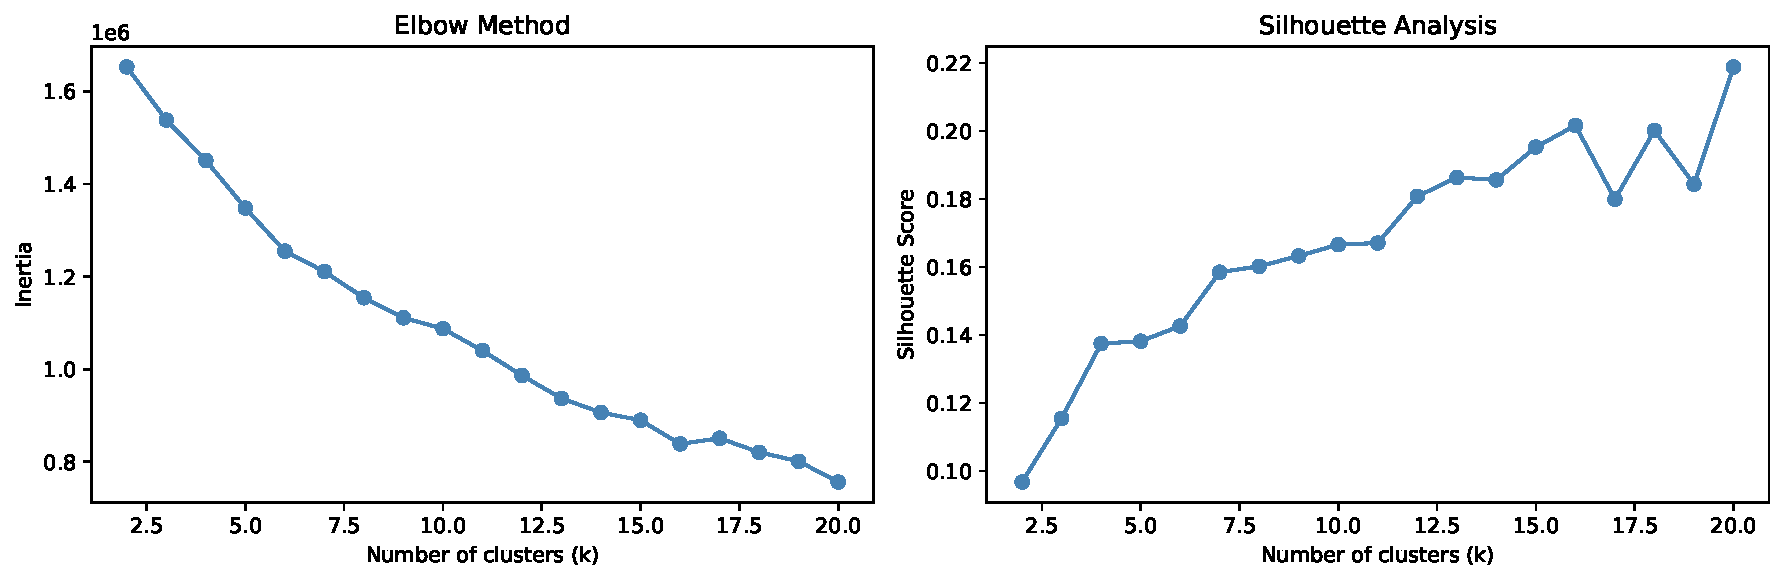
\includegraphics[width=0.7\linewidth]{files/5836668980c97017a580f41498802e7a.pdf}

\begin{verbatim}
Best k by silhouette score: 20
\end{verbatim}

\paragraph{Hierarchical clustering}

An alternative to k-means is \textbf{hierarchical clustering}, which builds a tree of clusters. This is particularly useful when you want to visualize the relationships between features at multiple scales.

\begin{verbatim}
# Use short features for clearer visualization
X_short_T = training_sample[features_short].values.T

# Compute hierarchical clustering
linkage_matrix = linkage(X_short_T, method='ward')

# Plot dendrogram
plt.figure(figsize=(10, 5))
dendrogram(linkage_matrix, labels=features_short, leaf_rotation=45)
plt.title('Hierarchical Clustering Dendrogram')
plt.ylabel('Distance')
plt.tight_layout()
plt.show()
\end{verbatim}

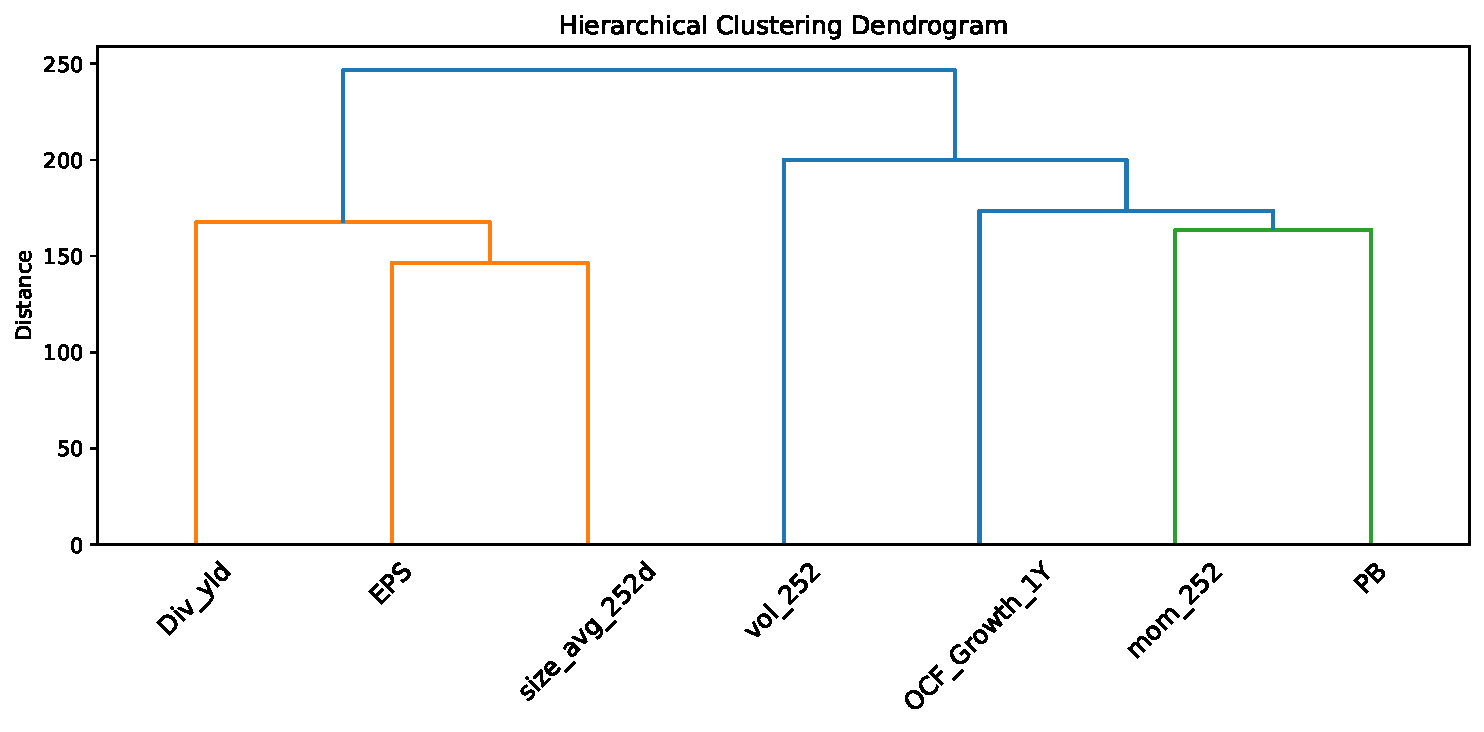
\includegraphics[width=0.7\linewidth]{files/47b87db651b6c23eaa1be356f69cee00.pdf}

\subsubsection{Nearest neighbors}

To the best of our knowledge, nearest neighbors are not used in large-scale portfolio choice applications. The reason is simple: computational cost. Nonetheless, the concept of neighbors is widespread in unsupervised learning and can be used locally in complement to interpretability tools. Theoretical results on k-NN relating to bounds for error rates on classification tasks can be found in section 6.2 of \cite{ripley2007pattern}. The rationale is the following. If:

\begin{enumerate}
\item the training sample is able to accurately span the distribution of $(\textbf{y}, \textbf{X})$; \textbf{and}
\item the testing sample follows the same distribution as the training sample (or close enough);
\end{enumerate}

then the neighborhood of one instance $\textbf{x}_i$ from the testing features computed on the training sample will yield valuable information on $y_i$.

In what follows, we thus seek to find neighbors of one particular instance $\textbf{x}_i$ (a $K$-dimensional row vector). Note that there is a major difference with the previous section: the clustering is intended at the observation level (row) and not at the predictor level (column).

Given a dataset with the same (corresponding) columns $\textbf{X}_{i,k}$, the neighbors are defined via a similarity measure (or distance)

\begin{equation}
\label{eq:D}
D(\textbf{x}_j,\textbf{x}_i)=\sum_{k=1}^Kc_k d_k(x_{j,k},x_{i,k}),
\end{equation}

where the distance functions $d_k$ can operate on various data types (numerical, categorical, etc.). For numerical values, $d_k(x_{j,k},x_{i,k})=(x_{j,k} -x_{i,k})^2$ or $d_k(x_{j,k},x_{i,k})=|x_{j,k} -x_{i,k}|$. For categorical values, we refer to the exhaustive survey by \cite{boriah2008similarity} which lists 14 possible measures. Finally the $c_k$ in Equation \ref{eq:D} allow some flexbility by weighting features. This is useful because both raw values ($x_{i,k}$ versus $x_{i,k'}$) or measure outputs ($d_k$ versus $d_{k'}$) can have different scales.

Once the distances are computed over the whole sample, they are ranked using indices $l_1^i, \dots, l_I^i$:
\begin{equation}
D\left(\textbf{x}_{l_1^i},\textbf{x}_i\right) \le D\left(\textbf{x}_{l_2^i},\textbf{x}_i\right) \le \dots, \le D\left(\textbf{x}_{l_I^i},\textbf{x}_i\right)
\end{equation}

The nearest neighbors are those indexed by $l_m^i$ for $m=1,\dots,k$. We leave out the case when there are problematic equalities of the type $D\left(\textbf{x}_{l_m^i},\textbf{x}_i\right)=D\left(\textbf{x}_{l_{m+1}^i},\textbf{x}_i\right)$ for the sake of simplicity and because they rarely occur in practice as long as there are sufficiently many numerical predictors.

Given these neighbors, it is now possible to build a prediction for the label side $y_i$. The rationale is straightforward: if $\textbf{x}_i$ is close to other instances $\textbf{x}_j$, then the label value $y_i$ should also be close to $y_j$ (under the assumption that the features carry some predictive information over the label $y$).

An intuitive prediction for $y_i$ is the following weighted average:
\begin{equation}
\hat{y}_i=\frac{\sum_{j\neq i} h(D(\textbf{x}_j,\textbf{x}_i)) y_j}{\sum_{j\neq i} h(D(\textbf{x}_j,\textbf{x}_i))},
\end{equation}
where $h$ is a decreasing function. Thus, the further $\textbf{x}_j$ is from $\textbf{x}_i$, the smaller the weight in the average. A typical choice for $h$ is $h(z)=e^{ -az}$ for some parameter $a>0$ that determines how penalizing the distance $D(\textbf{x}_j,\textbf{x}_i)$ is. Of course, the average can be taken in the set of $k$ nearest neighbors, in which case the $h$ is equal to zero beyond a particular distance threshold:
\begin{equation}
\hat{y}_i=\frac{\sum_{j \text{ neighbor}} h(D(\textbf{x}_j,\textbf{x}_i)) y_j}{\sum_{j \text{ neighbor}} h(D(\textbf{x}_j,\textbf{x}_i))}.
\end{equation}

A more agnostic rule is to take $h:=1$ over the set of neighbors and in this case, all neighbors have the same weight (see the old discussion by \cite{bailey1978note} in the case of classification). For classification tasks, the procedure involves a voting rule whereby the class with the most votes wins the contest, with possible tie-breaking methods. The interested reader can have a look at the short survey in \cite{bhatia2010survey}.

For the choice of optimal $k$, several complicated techniques and criteria exist (see, e.g., \cite{ghosh2006optimum} and \cite{hall2008choice}). Heuristic values often do the job pretty well. A rule of thumb is that $k=\sqrt{I}$ ($I$ being the total number of instances) is not too far from the optimal value, unless $I$ is exceedingly large.

Below, we illustrate this concept. We pick one date (31th of December 2006) and single out one asset. We then seek to find the $k=30$ stocks that are the closest to this asset at this particular date.

\begin{verbatim}
# Dataset for k-NN exercise
knn_data = data_ml[data_ml['date'] == '2006-12-31'].copy()

# Get first stock as target
first_stock = knn_data['fsym_id'].iloc[0]
knn_target = knn_data[knn_data['fsym_id'] == first_stock][features].values
knn_sample = knn_data[knn_data['fsym_id'] != first_stock][features].values

# Fit nearest neighbors model
nn_model = NearestNeighbors(n_neighbors=30, metric='euclidean')
nn_model.fit(knn_sample)

# Find neighbors
distances, indices = nn_model.kneighbors(knn_target)

print("Indices of the k=30 nearest neighbors:")
print(indices[0])
\end{verbatim}

\begin{verbatim}
Indices of the k=30 nearest neighbors:
[ 584  133   52  932 1153  657  982  236 1004   37  994  377  639  617
  709  589 1191 1011  813  622  873  691  914 1116  886 1047  418  219
 1010  607]
\end{verbatim}

Once the neighbors and distances are known, we can compute a prediction for the return of the target stock. We use the function $h(z)=e^{ -z}$ for the weighting of instances (via the distances).

\begin{verbatim}
# Get labels (returns) for neighbors
knn_sample_full = knn_data[knn_data['fsym_id'] != first_stock].reset_index(drop=True)
knn_labels = knn_sample_full.iloc[indices[0]]['R1M'].values

# Weighted prediction with h(z) = e^(-z)
weights = np.exp(-distances[0])
prediction = np.sum(knn_labels * weights) / np.sum(weights)

# True value
true_value = knn_data[knn_data['fsym_id'] == first_stock]['R1M'].values[0]

print(f"Prediction with h(z)=e^(-z): {prediction:.4f}")
print(f"True R1M value: {true_value:.4f}")
\end{verbatim}

\begin{verbatim}
Prediction with h(z)=e^(-z): 0.0430
True R1M value: -0.0262
\end{verbatim}

The prediction is neither very good, nor very bad (the sign may be correct!). However, note that this example cannot be used for predictive purposes because we use data from 2006-12-31 to predict a return at the same date. In order to avoid the forward-looking bias, the knn\_sample variable should be chosen from a prior point in time.

The above computations are fast (a handful of seconds at most), but hold for only one asset. In a $k$-NN exercise, each stock gets a customed prediction and the set of neighbors must be re-assessed each time. For $N$ assets, $N(N -1)/2$ distances must be evaluated. This is particularly costly in a backtest, especially when several parameters can be tested (the number of neighbors, $k$, or $a$ in the weighting function $h(z)=e^{ -az}$). When the investment universe is small (when trading indices for instance), \textit{k}-NN methods become computationally attractive (see for instance \cite{chen2017feature}).

\paragraph{Ball Tree and KD Tree for efficient k-NN}

For large datasets, scikit-learn provides optimized algorithms like Ball Tree and KD Tree that can significantly speed up nearest neighbor queries.

\begin{verbatim}
# Compare different algorithms
algorithms = ['brute', 'ball_tree', 'kd_tree']
times = {}

for algo in algorithms:
    nn = NearestNeighbors(n_neighbors=30, algorithm=algo)
    
    start = time.time()
    nn.fit(knn_sample)
    nn.kneighbors(knn_target)
    times[algo] = time.time() - start

print("Algorithm comparison (time in seconds):")
for algo, t in times.items():
    print(f"  {algo}: {t:.4f}s")
\end{verbatim}

\begin{verbatim}
Algorithm comparison (time in seconds):
  brute: 0.0012s
  ball_tree: 0.0041s
  kd_tree: 0.0017s
\end{verbatim}

\subsubsection{Anomaly detection with Isolation Forest}

An important application of unsupervised learning in finance is \textbf{anomaly detection}. Isolation Forest is an efficient algorithm that identifies anomalies by isolating observations. Anomalies are easier to isolate and thus have shorter path lengths in the tree structure.

\begin{verbatim}
# Fit Isolation Forest
iso_forest = IsolationForest(n_estimators=100, contamination=0.05, random_state=42)
anomaly_labels = iso_forest.fit_predict(X_train)

# Count anomalies
n_anomalies = np.sum(anomaly_labels == -1)
print(f"Number of anomalies detected: {n_anomalies} ({100*n_anomalies/len(X_train):.1f}%)")

# Visualize anomalies using PCA projection
X_pca = pca.transform(X_train)[:, :2]

plt.figure(figsize=(10, 6))
plt.scatter(X_pca[anomaly_labels == 1, 0], X_pca[anomaly_labels == 1, 1], 
            alpha=0.3, s=10, label='Normal', c='steelblue')
plt.scatter(X_pca[anomaly_labels == -1, 0], X_pca[anomaly_labels == -1, 1], 
            alpha=0.8, s=20, label='Anomaly', c='red')
plt.xlabel('PC1')
plt.ylabel('PC2')
plt.title('Anomaly Detection with Isolation Forest')
plt.legend()
plt.tight_layout()
plt.show()
\end{verbatim}

\begin{verbatim}
Number of anomalies detected: 11428 (5.0%)
\end{verbatim}

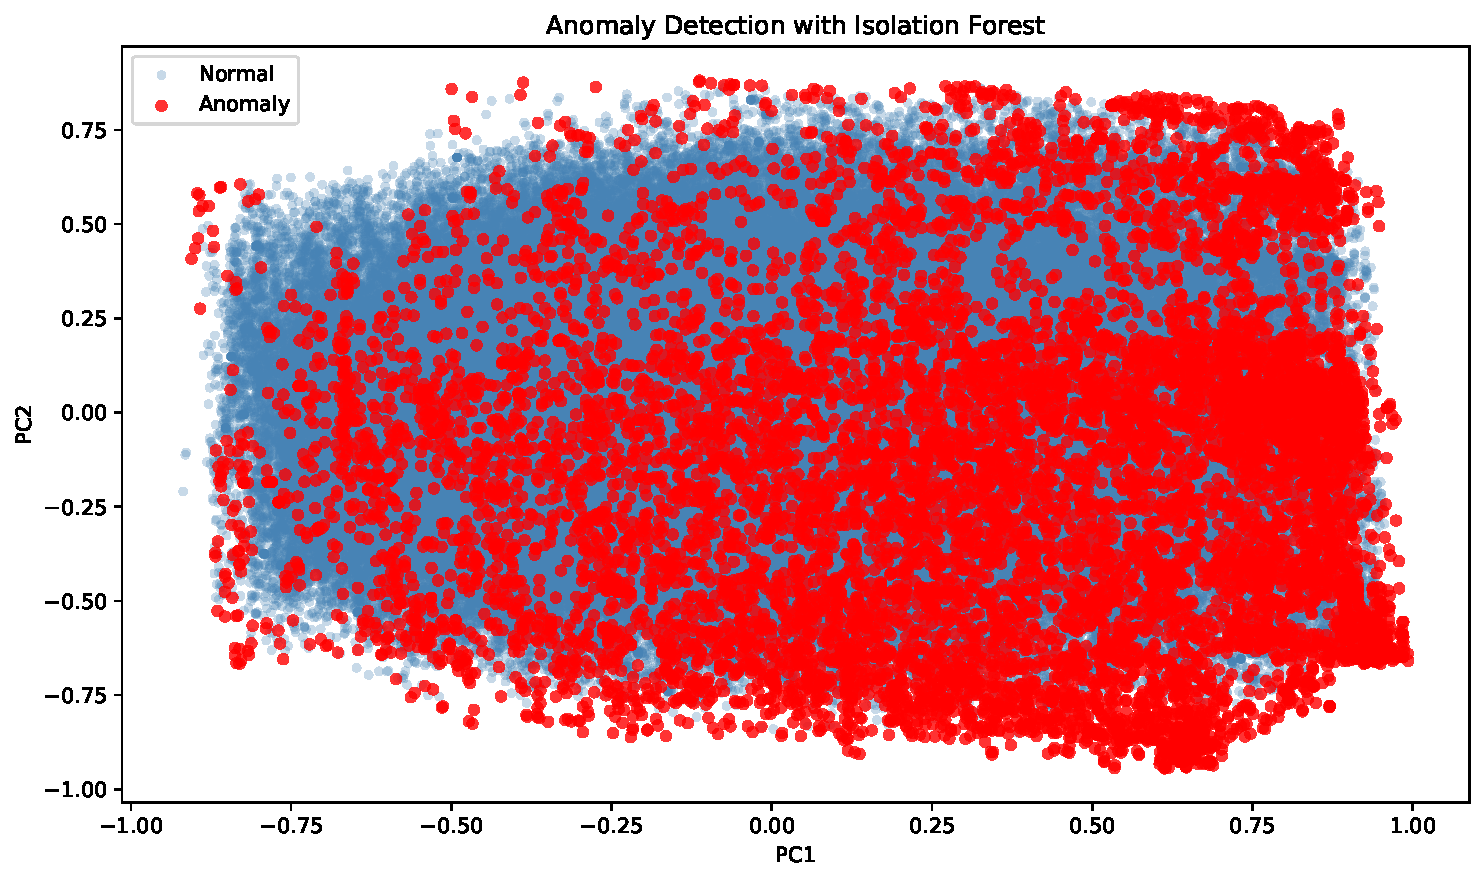
\includegraphics[width=0.7\linewidth]{files/5a1e7219de6798ee5ee6a7334f70395b.pdf}

\subsubsection{Coding exercise}

Code the compressed version of the data (narrow training sample) via the encoder part of the autoencoder.

\begin{verbatim}
# Solution: Use the encoder model to compress data
# The encoder was already built above:
# encoder_model = Model(inputs=input_layer, outputs=encoded)

# Compress the full training data
X_compressed_full = encoder_model.predict(X_train)

# Create a DataFrame with the compressed features
compressed_df = pd.DataFrame(
    X_compressed_full,
    columns=['AE1', 'AE2', 'AE3', 'AE4']
)

print("Compressed data shape:", compressed_df.shape)
print("\nFirst few rows:")
compressed_df.head()
\end{verbatim}

\begin{verbatim}
7143/7143 -------------------- 1s 153us/step
\end{verbatim}

\begin{verbatim}
Compressed data shape: (228548, 4)

First few rows:
\end{verbatim}

\bigskip\noindent
\begin{tabular}{p{\dimexpr 0.200\linewidth-2\tabcolsep}p{\dimexpr 0.200\linewidth-2\tabcolsep}p{\dimexpr 0.200\linewidth-2\tabcolsep}p{\dimexpr 0.200\linewidth-2\tabcolsep}p{\dimexpr 0.200\linewidth-2\tabcolsep}}
\toprule
 & AE1 & AE2 & AE3 & AE4 \\
\hline
0 & 0.028365 & 0.244199 & -0.137838 & -0.421712 \\
\hline
1 & 0.028082 & 0.244639 & -0.137827 & -0.421636 \\
\hline
2 & 0.027962 & 0.244831 & -0.137824 & -0.421603 \\
\hline
3 & 0.027390 & 0.245763 & -0.137814 & -0.421444 \\
\hline
4 & 0.027711 & 0.245270 & -0.137827 & -0.421528 \\
\hline
\bottomrule
\end{tabular}

\bigskip

\begin{verbatim}
# Compare compression quality: correlation between original and reconstructed
X_reconstructed = ae_model.predict(X_train)

# Compute correlation for each feature
correlations = []
for i, feat in enumerate(features_short):
    corr = np.corrcoef(X_train[:, i], X_reconstructed[:, i])[0, 1]
    correlations.append(corr)

print("Reconstruction quality (correlation original vs reconstructed):")
for feat, corr in zip(features_short, correlations):
    print(f"  {feat}: {corr:.4f}")

print(f"\nMean correlation: {np.mean(correlations):.4f}")
\end{verbatim}

\begin{verbatim}
7143/7143 -------------------- 1s 154us/step
\end{verbatim}

\begin{verbatim}
Reconstruction quality (correlation original vs reconstructed):
  Div_yld: 0.7822
  EPS: 0.7536
  size_avg_252d: 0.8594
  mom_252: 0.9732
  OCF_Growth_1Y: 0.9979
  PB: 0.8561
  vol_252: 0.8308

Mean correlation: 0.8648
\end{verbatim}

\subsection{Reinforcement learning}

Due to its increasing popularity within the Machine Learning community, we dedicate a chapter to reinforcement learning (RL). In 2019 only, more than 25 papers dedicated to RL have been submitted to (or updated on) arXiv under the \textbf{q:fin} (quantitative finance) classification. Applications to trading include \cite{xiong2018practical} and \cite{theate2020application}. Market microstructure is a focal framework (\cite{wei2019model}, \cite{ferreira2020reinforced}, \cite{karpe2020multi}).\newline
Moreover, an early survey of RL-based portfolios is compiled in \cite{sato2019model} (see also \cite{zhang2020deep}) and general financial applications are discussed in \cite{kolm2019modern}, \cite{meng2019reinforcement}, \cite{charpentier2020reinforcement} and \cite{mosavi2020comprehensive}. This shows again that RL has recently gained traction among the quantitative finance community.\footnote{Like neural networks, reinforcement learning methods have also been recently developed for derivatives pricing and hedging, see for instance \cite{kolm2019dynamic} and \cite{du2020deep}.}

While RL is a framework much more than a particular algorithm, its efficient application in portfolio management is not straightforward, as we will show. For a discussion on the generalization ability of RL algorithms, we refer to \cite{packer2018assessing} and \cite{ghosh2021generalization}.

\subsubsection{Theoretical layout}

\paragraph{General framework}

In this section, we introduce the core concepts of RL and follow relatively closely the notations (and layout) of
\cite{sutton2018reinforcement}, which is widely considered as a solid reference in the field, along with \cite{bertsekas2017dynamic}. One central tool in the field is called the \textbf{Markov Decision Process} (MDP, see Chapter 3 in \cite{sutton2018reinforcement}).

MDPs, like all RL frameworks, involve the interaction between an \textbf{agent} (e.g., a trader or portfolio manager) and an \textbf{environment} (e.g., a financial market). The agent performs \textbf{actions} that may alter the state of environment and gets a reward (possibly negative) for each action. This short sequence can be repeated an arbitrary number of times, as is shown in the figure below.

\begin{figure}[!htbp]
\centering
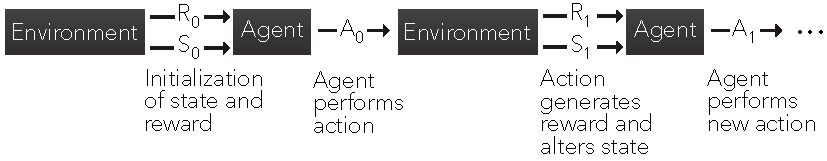
\includegraphics[width=0.7\linewidth]{files/MDP_scheme-eccd226b1f166ca23f97f5ac874f8889.pdf}
\caption[]{Scheme of Markov Decision Process. R, S and A stand for reward, state and action, respectively.}
\label{fig-mdpscheme}
\end{figure}

Given initialized values for the state of the environment ($S_0$) and reward (usually $R_0=0$), the agent performs an action (e.g., invests in some assets). This generates a reward $R_1$ (e.g., returns, profits, Sharpe ratio) and also a future state of the environment ($S_1$). Based on that, the agent performs a new action and the sequence continues. When the sets of states, actions and rewards are finite, the MDP is logically called \textit{finite}. In a financial framework, this is somewhat unrealistic and we discuss this issue later on. It nevertheless is not hard to think of simplified and discretized financial problems. For instance, the reward can be binary: win money versus lose money. In the case of only one asset, the action can also be dual: investing versus not investing. When the number of assets is sufficiently small, it is possible to set fixed proportions that lead to a reasonable number of combinations of portfolio choices, etc.

We pursue our exposé with finite MDPs; they are the most common in the literature and their formal treatment is simpler. The relative simplicity of MDPs helps grasp the concepts that are common to other RL techniques. As is often the case with Markovian objects, the key notion is that of \textbf{transition probability}:

\begin{equation}
\label{eq-transprob}
p(s',r|s,a)=\mathbb{P}\left[S_t=s',R_t=r | S_{t-1}=s,A_{t-1}=a \right],
\end{equation}

which is the probability of reaching state $s'$ and reward $r$ at time $t$, conditionally on being in state $s$ and performing action $a$ at time $t -1$. The finite sets of states and actions will be denoted with $\mathcal{S}$ and $\mathcal{A}$ henceforth.
Sometimes, this probability is averaged over the set of rewards which gives the following decomposition:

\begin{equation}
\label{eq-transprob2}
\begin{aligned}
\sum_r rp(s',r|s,a)&=\mathcal{P}_{ss'}^a \mathcal{R}_{ss'}^a, \quad \text{ where } \\
\mathcal{P}_{ss'}^a &=\mathbb{P}\left[S_t=s' | S_{t-1}=s,A_{t-1}=a \right],  \quad \text{ and } \\
 \mathcal{R}_{ss'}^a &= \mathbb{E}\left[R_t | S_{t-1}=s,S_t=s', A_{t-1}=a \right].
\end{aligned}
\end{equation}

The goal of the agent is to maximize some function of the stream of rewards. This gain is usually defined as

\begin{equation}
\label{eq-gain}
\begin{aligned}
G_t&=\sum_{k=0}^T\gamma^kR_{t+k+1} \\
&=R_{t+1} +\gamma G_{t+1},
\end{aligned}
\end{equation}

i.e., it is a discounted version of the reward, where the discount factor is $\gamma \in (0,1]$. The horizon $T$ may be infinite, which is why $\gamma$ was originally introduced. Assuming the rewards are bounded, the infinite sum may diverge for $\gamma=1$. That is the case if rewards don't decrease with time and there is no reason why they should.
When $\gamma <1$ and rewards are bounded, convergence is assured. When $T$ is finite, the task is called \textit{episodic} and, otherwise, it is said to be \textit{continuous}.

In RL, the focal unknown to be optimized or learned is the \textbf{policy} $\pi$, which drives the actions of the agent. More precisely, $\pi(a,s)=\mathbb{P}[A_t=a|S_t=s]$, that is, $\pi$ equals the probability of taking action $a$ if the state of the environment is $s$. This means that actions are subject to randomness, just like for mixed strategies in game theory. While this may seem disappointing because an investor would want to be sure to take \textit{the} best action, it is also a good reminder that the best way to face random outcomes may well be to randomize actions as well.

Finally, in order to try to determine the \textit{best} policy, one key indicator is the so-called value function:

\begin{equation}
\label{eq-RLvalue}
v_\pi(s)=\mathbb{E}_\pi\left[ G_t | S_t=s \right],
\end{equation}

where the time index $t$ is not very relevant and omitted in the notation of the function. The index $\pi$ under the expectation operator $\mathbb{E}[\cdot]$ simply indicates that the average is taken when the policy $\pi$ is enforced. The value function is simply equal to the average gain conditionally on the state being equal to $s$. In financial terms, this is equivalent to the average profit if the agent takes actions driven by $\pi$ when the market environment is $s$. More generally, it is also possible to condition not only on the state, but also on the action taken. We thus introduce the $q_\pi$ action-value function:

\begin{equation}
\label{eq-RLQ}
q_\pi(s,a)=\mathbb{E}_\pi\left[ G_t | S_t=s, \ A_t=a \right].
\end{equation}

The $q_\pi$ function is highly important because it gives the average gain when the state and action are fixed. Hence, if the current state is known, then one obvious choice is to select the action for which $q_\pi(s,\cdot)$ is the highest. Of course, this is the best solution if the optimal value of $q_\pi$ is known, which is not always the case in practice. The value function can easily be accessed via $q_\pi$: $v_\pi(s)=\sum_a \pi(a,s)q_\pi(s,a)$.

The optimal $v_\pi$ and $q_\pi$ are straightforwardly defined as
\begin{equation}
v_*(s)=\underset{\pi}{\max} \, v_\pi(s), \ \forall s\in \mathcal{S}, \quad \text{ and } \quad q_*(s,a) =\underset{\pi}{\max} \, q_\pi(s,a), \ \forall (s,a)\in \mathcal{S}\times \mathcal{A}.
\end{equation}

If only $v_*(s)$ is known, then the agent must span the set of actions and find those that yield the maximum value for any given state $s$.

Finding these optimal values is a very complicated task and many articles are dedicated to solving this challenge. One reason why finding the best $q_\pi(s,a)$ is difficult is because it depends on two elements ($s$ and $a$) on one side and $\pi$ on the other. Usually, for a fixed policy $\pi$, it can be time consuming to evaluate $q_\pi(s,a)$ for a given stream of actions, states and rewards. Once $q_\pi(s,a)$ is estimated, then a new policy $\pi'$ must be tested and evaluated to determine if it is better than the original one.
Thus, this iterative search for a good policy can take long. For more details on policy improvement and value function updating, we recommend chapter 4 of \cite{sutton2018reinforcement} which is dedicated to dynamic programming.

\paragraph{Q-learning}

An interesting shortcut to the problem of finding $v_*(s)$ and $q_*(s,a)$ is to remove the dependence on the policy. Consequently, there is then of course no need to iteratively improve it. The central relationship that is required to do this is the so-called Bellman equation that is satisfied by $q_\pi(s,a)$. We detail its derivation below. First of all, we recall that

\$\$
{\textbackslash}begin\{aligned\}
q\_{\textbackslash}pi(s,a) \&= {\textbackslash}mathbb\{E\}\textit{{\textbackslash}pi[G\_t|S\_t=s,A\_t=a] {\textbackslash}
\&= {\textbackslash}mathbb\{E\}}{\textbackslash}pi[R\_\{t+1\}+ {\textbackslash}gamma G\_\{t+1\}|S\_t=s,A\_t=a],
{\textbackslash}end\{aligned\}

\$\$

where the second equality stems from Equation \ref{eq-gain}. The expression $\mathbb{E}_\pi[R_{t+1}|S_t=s,A_t=a]$ can be further decomposed. Since the expectation runs over $\pi$, we need to sum over all possible actions $a'$ and states $s'$ and resort to $\pi(a',s')$. In addition, the sum on the $s'$ and $r$ arguments of the probability $p(s',r|s,a)=\mathbb{P}\left[S_{t+1}=s',R_{t+1}=r | S_t=s,A_t=a \right]$ gives access to the distribution of the random couple $(S_{t+1},R_{t+1})$ so that in the end $\mathbb{E}_\pi[R_{t+1}|S_t=s,A_t=a]=\sum_{a', r,s'}\pi(a',s')p(s',r|s,a)  r$. A similar reasoning applies to the second portion of $q_\pi$ and:

\begin{equation}
\label{eq-bellman}
\begin{aligned}
q_\pi(s,a) &=\sum_{a',r, s'}\pi(a',s')p(s',r|s,a) \left[ r+\gamma q_\pi(s',a')\right].
\end{aligned}
\end{equation}

This equation links $q_\pi(s,a)$ to the future $q_\pi(s',a')$ from the states and actions $(s',a')$ that are accessible from $(s,a)$.

Notably, Equation \ref{eq-bellman} is also true for the optimal action-value function $q_*=\underset{\pi}{\max} \, q_\pi(s,a)$:

\begin{equation}
\label{eq-bellmanq}
\begin{aligned}
q_*(s,a) &= \underset{a'}{\max} \sum_{r,s'}p(s',r|s,a) \left[ r+\gamma q_*(s',a')\right], \\ 
&= \mathbb{E}_{\pi^*}[r|s,a]+ \gamma \, \sum_{r,s'}p(s',r|s,a) \left(  \underset{a'}{\max}  q_*(s',a') \right)
\end{aligned}
\end{equation}

because one optimal policy is one that maximizes $q_\pi(s,a)$, for a given state $s$ and over all possible actions $a$. This expression is central to a cornerstone algorithm in reinforcement learning called $Q$-learning (the formal proof of convergence is outlined in \cite{watkins1992q}). In $Q$-learning, the state-action function no longer depends on policy and is written with capital $Q$. The process is the following:

Initialize values $Q(s,a)$ for all states $s$ and actions $a$. For each episode:\newline
\begin{equation}
(\textbf{QL}) \quad \left\{
\begin{array}{l}
\text{0. Initialize state } S_0 \text{ and for each iteration } i \text{ until the end of the episode;}   \\
\text{1. observe state } s_i;    \\
\text{2. perform action } a_i \text{(depending on } Q);   \\
\text{3. receive reward }r_{i+1} \text{ and observe state } s_{i+1};  \\
\text{4. Update } Q \text{ as follows: }
\end{array} \right.
\end{equation}

\begin{equation}
\label{eq-QLupdate}
Q_{i+1}(s_i,a_i) \longleftarrow Q_i(s_i,a_i) + \eta  \left(\underbrace{r_{i+1}+\gamma \, \underset{a}{\max} \, Q_i(s_{i+1},a)}_{\text{echo of Bellman eq.}}-Q_i(s_i,a_i) \right)
\end{equation}

The underlying reason this update rule works can be linked to fixed point theorems of contraction mappings. If a function $f$ satisfies $|f(x) -f(y)|< \delta |x -y|$ (Lipshitz continuity), then a fixed point $z$ satisfying $f(z)=z$ can be iteratively obtained via $z \leftarrow f(z)$. This updating rule converges to the fixed point. Equation \ref{eq-bellmanq} can be solved using a similar principle, except that a learning rate $\eta$ slows the learning process but also technically ensures convergence under technical assumptions.

More generally, Equation \ref{eq-QLupdate} has a form that is widespread in reinforcement learning that is summarized in Equation (2.4) of \cite{sutton2018reinforcement}:

\begin{equation}
\label{eq-RLeq}
\text{New estimate} \leftarrow \text{Old estimate + Step size (}i.e., \text{ learning rate)} \times (\text{Target - Old estimate}),
\end{equation}

where the last part can be viewed as an error term. Starting from the old estimate, the new estimate therefore goes in the `right' (or sought) direction, modulo a discount term that makes sure that the magnitude of this direction is not too large. The update rule in Equation \ref{eq-QLupdate} is often referred to as `\textit{temporal difference}' learning because it is driven by the improvement yielded by estimates that are known at time $t+1$ (target) versus those known at time $t$.

One important step of the \textit{Q}-learning sequence (\textbf{QL}) is the second one where the action $a_i$ is picked. In RL, the best algorithms combine two features: \textbf{exploitation} and \textbf{exploration}. Exploitation is when the machine uses the current information at its disposal to choose the next action. In this case, for a given state $s_i$, it chooses the action $a_i$ that maximizes the expected reward $Q_i(s_i,a_i)$. While obvious, this choice is not optimal if the current function $Q_i$ is relatively far from the \textit{true} $Q$. Repeating the locally optimal strategy is likely to favor a limited number of actions, which will narrowly improve the accuracy of the $Q$ function.

In order to gather new information stemming from actions that have not been tested much (but that can potentially generate higher rewards), exploration is needed. This is when an action $a_i$ is chosen randomly. The most common way to combine these two concepts is called $\epsilon$-greedy exploration. The action $a_i$ is assigned according to:

\begin{equation}
\label{eq-egreedy}
a_i=\left\{ \begin{array}{c l}
\underset{a}{\text{argmax}} \ Q_i(s_i,a) & \text{ with probability } 1-\epsilon \\
\text{randomly (uniformly) over } \mathcal{A} & \text{ with probability } \epsilon
\end{array}\right. .
\end{equation}

Thus, with probability $\epsilon$, the algorithm explores and with probability $1 -\epsilon$, it exploits the current knowledge of the expected reward and picks the best action. Because all actions have a non-zero probability of being chosen, the policy is called ``soft''. Indeed, then best action has a probability of selection equal to $1 -\epsilon(1 -\text{card}(\mathcal{A})^{ -1})$, while all other actions are picked with probability $\epsilon/\text{card}(\mathcal{A})$.

\paragraph{SARSA}

In $Q$-learning, the algorithm seeks to find the action-value function of the optimal policy. Thus, the policy that is followed to pick actions is different from the one that is learned (via $Q$). Such algorithms are called \textit{off-policy}. \textit{On-policy} algorithms seek to improve the estimation of the action-value function $q_\pi$ by continuously acting according to the policy $\pi$. One canonical example of on-policy learning is the SARSA method which requires two consecutive states and actions \textbf{SA}R\textbf{SA}. The way the quintuple $(S_t,A_t,R_{t+1}, S_{t+1}, A_{t+1})$ is processed is presented below.

The main difference between $Q$ learning and SARSA is the update rule. In SARSA, it is given by

\begin{equation}
\label{eq-SARSAupdate}
Q_{i+1}(s_i,a_i) \longleftarrow Q_i(s_i,a_i) + \eta  \left(r_{i+1}+\gamma \, Q_i(s_{i+1},a_{i+1})-Q_i(s_i,a_i) \right)
\end{equation}

The improvement comes only from the \textbf{local} point $Q_i(s_{i+1},a_{i+1})$ that is based on the new states and actions ($s_{i+1},a_{i+1}$), whereas in $Q$-learning, it comes from all possible actions of which only the best is retained $\underset{a}{\max} \, Q_i(s_{i+1},a)$.

A more robust but also more computationally demanding version of SARSA is \textit{expected} SARSA in which the target $Q$ function is averaged over all actions:

\begin{equation}
\label{eq-exSARSAupdate}
Q_{i+1}(s_i,a_i) \longleftarrow Q_i(s_i,a_i) + \eta  \left(r_{i+1}+\gamma \, \sum_a \pi(a,s_{i+1}) Q_i(s_{i+1},a) -Q_i(s_i,a_i) \right)
\end{equation}

Expected SARSA is less volatile than SARSA because the latter is strongly impacted by the random choice of $a_{i+1}$. In expected SARSA, the average smoothes the learning process.

\subsubsection{The curse of dimensionality}

Let us first recall that reinforcement learning is a framework that is not linked to a particular algorithm. In fact, different tools can very well co-exist in a RL task (AlphaGo combined both tree methods and neural networks, see \cite{silver2016mastering}). Nonetheless, any RL attempt will always rely on the three key concepts: the states,  actions and rewards. In factor investing, they are fairly easy to identify, though there is always room for interpretation. Actions are evidently defined by portfolio compositions. The states can be viewed as the current values that describe the economy: as a first-order approximation, it can be assumed that the feature levels fulfill this role (possibly conditioned or complemented with macro-economic data). The rewards are even more straightforward. Returns or any relevant performance metric\footnote{e.g., Sharpe ratio which is for instance used in \cite{moody1998performance}, \cite{bertoluzzo2012testing} and \cite{aboussalah2020continuous} or drawdown-based ratios, as in \cite{almahdi2017adaptive}.} can account for rewards.

A major problem lies in the dimensionality of both states and actions. Assuming an absence of leverage (no negative weights), the actions take values on the simplex

\begin{equation}
\label{eq-simplex}
\mathbb{S}_N=\left\{ \mathbf{x} \in \mathbb{R}^N\left|\sum_{n=1}^Nx_n=1, \ x_n\ge 0, \ \forall n=1,\dots,N \right.\right\}
\end{equation}

and assuming that all features have been uniformized, their space is $[0,1]^{NK}$. Needless to say, the dimensions of both spaces are numerically impractical.

A simple solution to this problem is discretization: each space is divided into a small number of categories. Some authors do take this route. In \cite{yang2018investor}, the state space is discretized into three values depending on volatility, and actions are also split into three categories. \cite{bertoluzzo2012testing}, \cite{xiong2018practical} and \cite{taghian2020learning} also choose three possible actions (buy, hold, sell). In \cite{almahdi2019constrained}, the learner is expected to yield binary signals for buying or shorting. \cite{garcia2019continuous} consider a larger state space (8 elements) but restrict the action set to 3 options.\footnote{Some recent papers consider arbitrary weights (e.g., \cite{jiang2017deep} and \cite{yu2019model}) for a limited number of assets.} In terms of the state space, all articles assume that the state of the economy is determined by prices (or returns).

One strong limitation of these approaches is the marked simplification they imply. Realistic discretizations are numerically intractable when investing in multiple assets. Indeed, splitting the unit interval in $h$ points yields $h^{NK}$ possibilities for feature values. The number of options for weight combinations is exponentially increasing with $N$. As an example: just 10 possible values for 10 features of 10 stocks yield 10\textsuperscript{100} permutations.

The problems mentioned above are of course not restricted to portfolio construction. Many solutions have been proposed to solve Markov Decision Processes in continuous spaces. We refer for instance to Section 4 in \cite{powell2011review} for a review of early methods (outside finance).

This curse of dimensionality is accompanied by the fundamental question of training data. Two options are conceivable: market data versus simulations. Under a given controlled generator of samples, it is hard to imagine that the algorithm will beat the solution that maximizes a given utility function. If anything, it should converge towards the static optimal solution under a stationary data generating process (see, e.g., \cite{chaouki2020deep} for trading tasks), which is by the way a very strong modelling assumption.

This leaves market data as a preferred solution but even with large datasets, there is little chance to cover all the (actions, states) combinations mentioned above. Characteristics-based datasets have depths that run through a few decades of monthly data, which means several hundreds of time-stamps at most. This is by far too limited to allow for a reliable learning process. It is always possible to generate synthetic data (as in \cite{yu2019model}), but it is unclear that this will solidly improve the performance of the algorithm.

\subsubsection{Policy gradient}

\paragraph{Principle}

Beyond the discretization of action and state spaces, a powerful trick is \textbf{parametrization}. When $a$ and $s$ can take discrete values, action-value functions must be computed for all pairs $(a,s)$, which can be prohibitively cumbersome. An elegant way to circumvent this problem is to assume that the policy is driven by a relatively modest number of parameters. The learning process is then focused on optimizing this set of parameters $\boldsymbol{\theta}$. We then write $\pi_{\boldsymbol{\theta}}(a,s)$ for the probability of choosing action $a$ in state $s$. One intuitive way to define $\pi_{\boldsymbol{\theta}}(a,s)$ is to resort to a soft-max form:

\begin{equation}
\label{eq-policyex}
\pi_{\boldsymbol{\theta}}(a,s) = \frac{e^{\boldsymbol{\theta}'\textbf{h}(a,s)}}{\sum_{b}e^{\boldsymbol{\theta}'\textbf{h}(b,s)}},
\end{equation}

where the output of function $\textbf{h}(a,s)$, which has the same dimension as $\boldsymbol{\theta}$ is called a feature vector representing the pair $(a,s)$. Typically, $\textbf{h}$ can very well be a simple neural network with two input units and an output dimension equal to the length of $\boldsymbol{\theta}$.

One desired property for $\pi_{\boldsymbol{\theta}}$ is that it be differentiable with respect to $\boldsymbol{\theta}$ so that $\boldsymbol{\theta}$ can be improved via some gradient method. The most simple and intuitive results about policy gradients are known in the case of episodic tasks (finite horizon) for which it is sought to maximize the average gain $\mathbb{E}_{\boldsymbol{\theta}}[G_t]$ where the gain is defined in Equation \ref{eq-gain}. The expectation is computed according to a particular policy that depends on $\boldsymbol{\theta}$, this is why we use a simple subscript. One central result is the so-called policy gradient theorem which states that

\begin{equation}
\label{eq-PGT}
\nabla \mathbb{E}_{\boldsymbol{\theta}}[G_t]=\mathbb{E}_{\boldsymbol{\theta}} \left[G_t\frac{\nabla \pi_{\boldsymbol{\theta}}}{\pi_{\boldsymbol{\theta}}} \right].
\end{equation}

This result can then be used for \textbf{gradient ascent}: when seeking to maximize a quantity, the parameter change must go in the upward direction:

\begin{equation}
\label{eq-ascent}
\boldsymbol{\theta} \leftarrow \boldsymbol{\theta} + \eta \nabla \mathbb{E}_{\boldsymbol{\theta}}[G_t].
\end{equation}

This simple update rule is known as the \textbf{REINFORCE} algorithm. One improvement of this simple idea is to add a baseline, and we refer to section 13.4 of \cite{sutton2018reinforcement} for a detailed account on this topic.

\paragraph{Extensions}

A popular extension of REINFORCE is the so-called \textbf{actor-critic} (AC) method which combines policy gradient with $Q$- or $v$-learning. The AC algorithm can be viewed as some kind of mix between policy gradient and SARSA. A central requirement is that the state-value function $v(\cdot)$ be a differentiable function of some parameter vector $\textbf{w}$ (it is often taken to be a neural network). The update rule is then

\begin{equation}
\label{eq-ascentAC}
\boldsymbol{\theta} \leftarrow \boldsymbol{\theta} + \eta \left(R_{t+1}+\gamma v(S_{t+1},\textbf{w})-v(S_t,\textbf{w}) \right)\frac{\nabla \pi_{\boldsymbol{\theta}}}{\pi_{\boldsymbol{\theta}}},
\end{equation}

but the trick is that the vector $\textbf{w}$ must also be updated. The actor is the policy side which is what drives decision making. The critic side is the value function that evaluates the actor's performance. As learning progresses (each time both sets of parameters are updated), both sides improve. The exact algorithmic formulation is a bit long and we refer to Section 13.5 in \cite{sutton2018reinforcement} for the precise sequence of steps of AC.

Another interesting application of parametric policies is outlined in \cite{aboussalah2020continuous}. In their article, the authors define a trading policy that is based on a recurrent neural network. Thus, the parameter $\boldsymbol{\theta}$ in this case encompasses all weights and biases in the network.

Another favorable feature of parametric policies is that they are compatible with continuous sets of actions. Beyond the form \ref{eq-policyex}, there are other ways to shape $\pi_{\boldsymbol{\theta}}$. If $\mathcal{A}$ is a subset of $\mathbb{R}$, and $f_{\boldsymbol{\Omega}}$ is a density function with parameters $\boldsymbol{\Omega}$, then a candidate form for $\pi_{\boldsymbol{\theta}}$ is

\begin{equation}
\label{eq-parpol}
\pi_{\boldsymbol{\theta}} = f_{\boldsymbol{\Omega}(s,\boldsymbol{\theta})}(a),
\end{equation}

in which the parameters $\boldsymbol{\Omega}$ are in turn functions of the states and of the underlying (second order) parameters $\boldsymbol{\theta}$.

While the Gaussian distribution (see section 13.7 in \cite{sutton2018reinforcement}) is often a preferred choice, they would require some processing to lie inside the unit interval. One easy way to obtain such values is to apply the normal cumulative distribution function to the output. In \cite{wang2019continuous}, the multivariate Gaussian policy is theoretically explored, but it assumes no constraint on weights.

Some natural parametric distributions emerge as alternatives. If only one asset is traded, then the Bernoulli distribution can be used to determine whether or not to buy the asset. If a riskless asset is available, the beta distribution offers more flexibility because the values for the proportion invested in the risky asset span the whole interval; the remainder can be invested into the safe asset. When many assets are traded, things become more complicated because of the budget constraint. One ideal candidate is the Dirichlet distribution because it is defined on a simplex (see Equation \ref{eq-simplex}):
\begin{equation}
f_{\boldsymbol{\alpha}}(w_1,\dots,w_n)=\frac{1}{B(\boldsymbol{\alpha})}\prod_{n=1}^Nw_n^{\alpha_n-1},
\end{equation}
where $B(\boldsymbol{\alpha})$ is the multinomial beta function:
\begin{equation}
B(\boldsymbol{\alpha})=\frac{\prod_{n=1}^N\Gamma(\alpha_n)}{\Gamma\left(\sum_{n=1}^N\alpha_n \right)}.
\end{equation}

If we set $\pi=\pi_{\boldsymbol{\alpha}}=f_{\boldsymbol{\alpha}}$, the link with factors or characteristics can be coded through ${\boldsymbol{\alpha}}$ via a linear form:

\begin{equation}
(\textbf{F1}) \quad  \alpha_{n,t}=\theta_{0,t} + \sum_{k=1}^K \theta_{t}^{(k)}x_{t,n}^{(k)},
\end{equation}

which is highly tractable, but may violate the condition that $\alpha_{n,t}>0$ for some values of $\theta_{k,t}$. Indeed, during the learning process, an update in $\boldsymbol{\theta}$ might yield values that are out of the feasible set of $\boldsymbol{\alpha}_t$. In this case, it is possible to resort to a trick that is widely used in online learning (see, e.g., section 2.3.1 in \cite{hoi2018online}). The idea is simply to find the acceptable solution that is closest to the suggestion from the algorithm. If we call $\boldsymbol{\theta}^*$ the result of an update rule from a given algorithm, then the closest feasible vector is

\begin{equation}
\boldsymbol{\theta}= \underset{\textbf{z} \in \Theta(\textbf{x}_t)}{\min} ||\boldsymbol{\theta}^*-\textbf{z}||^2,
\end{equation}

where $||\cdot||$ is the Euclidean norm and $\Theta(\textbf{x}_t)$ is the feasible set, that is, the set of vectors $\boldsymbol{\theta}$ such that the $\alpha_{n,t}=\theta_{0,t} + \sum_{k=1}^K \theta_{t}^{(k)}x_{t,n}^{(k)}$ are all non-negative.

A second option for the form of the policy, $\pi^2_{\boldsymbol{\theta}_t}$, is slightly more complex but remains always valid (i.e., has positive $\alpha_{n,t}$ values):

\begin{equation}
(\textbf{F2}) \quad  \alpha_{n,t}=\exp \left(\theta_{0,t} + \sum_{k=1}^K \theta_{t}^{(k)}x_{t,n}^{(k)}\right),
\end{equation}

which is simply the exponential of the first version. With some algebra, it is possible to derive the policy gradients. The policies $\pi^j_{\boldsymbol{\theta}_t}$ are defined by the Equations $(\textbf{Fj})$ above. Let $\digamma$ denote the digamma function. Let $\textbf{1}$ denote the $\mathbb{R}^N$ vector of all ones. We have

\begin{equation}
\begin{aligned}
\frac{\nabla_{\boldsymbol{\theta}_t} \pi^1_{\boldsymbol{\theta}_t}}{\pi^1_{\boldsymbol{\theta}_t}}&= \sum_{n=1}^N \left( \digamma \left( \textbf{1}'\textbf{X}_t\boldsymbol{\theta}_t \right) - \digamma(\textbf{x}_{t,n}\boldsymbol{\theta}_t) + \ln w_n \right) \textbf{x}_{t,n}' \\
\frac{\nabla_{\boldsymbol{\theta}_t} \pi^2_{\boldsymbol{\theta}_t}}{\pi^2_{\boldsymbol{\theta}_t}}&= \sum_{n=1}^N \left( \digamma \left( \textbf{1}'e^{\textbf{X}_{t}\boldsymbol{\theta}_t} \right) - \digamma(e^{\textbf{x}_{t,n}\boldsymbol{\theta}_t}) + \ln w_n \right) e^{\textbf{x}_{t,n}\boldsymbol{\theta}_t} \textbf{x}_{t,n}' 
\end{aligned}
\end{equation}

where $e^{\textbf{X}}$ is the element-wise exponential of a matrix $\textbf{X}$.

The allocation can then either be made by direct sampling, or using the mean of the distribution $(\textbf{1}'\boldsymbol{\alpha})^{ -1}\boldsymbol{\alpha}$. Lastly, a technical note: Dirichlet distributions can only be used for small portfolios because the scaling constant in the density becomes numerically intractable for large values of $N$ (e.g., above 50). More details on this idea are laid out in \cite{andre2020dirichlet}.

\subsubsection{Simple examples}

\paragraph{Setup and Imports}

\begin{verbatim}
import numpy as np
import pandas as pd
import matplotlib.pyplot as plt
import seaborn as sns
from collections import defaultdict
import warnings
warnings.filterwarnings('ignore')

# Set plotting style
plt.style.use('seaborn-v0_8-whitegrid')
sns.set_palette("husl")

# Building the data
from data_build import generate_data
data_ml, features, features_short, returns, stock_ids, stock_ids_short = generate_data()
\end{verbatim}

\paragraph{Q-learning with simulations}

To illustrate the gist of the problems mentioned above, we propose two implementations of $Q$-learning. For simplicity, the first one is based on simulations. This helps understand the learning process in a simplified framework. We consider two assets: one risky and one riskless, with return equal to zero. The returns for the risky process follow an autoregressive model of order one (AR(1)): $r_{t+1}=a+\rho r_t+\epsilon_{t+1}$ with $|\rho|<1$ and $\epsilon$ following a standard white noise with variance $\sigma^2$. In practice, individual (monthly) returns are seldom autocorrelated, but adjusting the autocorrelation helps understand if the algorithm learns correctly (see exercise below).

The environment consists only in observing the past return $r_t$. Since we seek to estimate the $Q$ function, we need to discretize this state variable. The simplest choice is to resort to a binary variable: equal to -1 (negative) if $r_t<0$ and to +1 (positive) if $r_t\ge 0$. The actions are summarized by the quantity invested in the risky asset. It can take 5 values: 0 (risk-free portfolio), 0.25, 0.5, 0.75 and 1 (fully invested in the risky asset). This is for instance the same choice as in \cite{pendharkar2018trading}.

Below we implement a simple Q-learning algorithm from scratch in Python. The landscape of Python libraries for RL is richer than R, with options like \textbf{Stable-Baselines3}, \textbf{RLlib}, and \textbf{Gymnasium} (formerly OpenAI Gym). However, for pedagogical purposes and to match the simplicity of the original example, we implement Q-learning directly.

\begin{verbatim}
class QLearningAgent:
    """
    A simple Q-learning agent for tabular environments.
    """
    def __init__(self, states, actions, alpha=0.1, gamma=0.7, epsilon=0.1):
        """
        Initialize the Q-learning agent.
        
        Parameters:
        -----------
        states : list
            List of possible states
        actions : list
            List of possible actions
        alpha : float
            Learning rate (eta in the equations)
        gamma : float
            Discount factor for future rewards
        epsilon : float
            Exploration rate for epsilon-greedy policy
        """
        self.states = states
        self.actions = actions
        self.alpha = alpha
        self.gamma = gamma
        self.epsilon = epsilon
        
        # Initialize Q-table with zeros
        self.Q = {s: {a: 0.0 for a in actions} for s in states}
    
    def choose_action(self, state):
        """Choose action using epsilon-greedy policy."""
        if np.random.random() < self.epsilon:
            # Explore: random action
            return np.random.choice(self.actions)
        else:
            # Exploit: best action based on Q-values
            return max(self.actions, key=lambda a: self.Q[state][a])
    
    def update(self, state, action, reward, next_state):
        """Update Q-value using the Q-learning update rule."""
        # Q-learning update (Equation eq-QLupdate)
        best_next_q = max(self.Q[next_state].values())
        td_target = reward + self.gamma * best_next_q
        td_error = td_target - self.Q[state][action]
        self.Q[state][action] += self.alpha * td_error
    
    def train_on_data(self, data):
        """
        Train the agent on a dataset.
        
        Parameters:
        -----------
        data : pd.DataFrame
            DataFrame with columns: state, action, reward, new_state
        """
        for _, row in data.iterrows():
            self.update(row['state'], row['action'], row['reward'], row['new_state'])
    
    def get_policy(self):
        """Return the best action for each state."""
        return {s: max(self.actions, key=lambda a: self.Q[s][a]) for s in self.states}
    
    def get_q_table(self):
        """Return Q-table as a DataFrame."""
        return pd.DataFrame(self.Q).T
\end{verbatim}

Now let's generate the simulated data with an AR(1) process and train our Q-learning agent.

\begin{verbatim}
# Set random seed for reproducibility
np.random.seed(42)

# Parameters for AR(1) simulation
n_sample = 10**5           # Number of samples to be generated
rho = 0.8                  # Autoregressive parameter
sd = 0.4                   # Std. dev. of noise
a = 0.06 * rho             # Scaled mean of returns

# Generate AR(1) returns
def simulate_ar1(n, rho, a, sd):
    """Simulate AR(1) process: r_{t+1} = a + rho * r_t + epsilon_{t+1}"""
    returns = np.zeros(n)
    returns[0] = a / (1 - rho)  # Start at unconditional mean
    epsilon = np.random.normal(0, sd, n)
    for t in range(1, n):
        returns[t] = a + rho * returns[t-1] + epsilon[t]
    return returns

# Generate returns
returns_sim = simulate_ar1(n_sample, rho, a, sd)

# Create dataset for Q-learning
# Random actions: 0, 0.25, 0.5, 0.75, 1.0
actions = np.round(np.random.uniform(0, 1, n_sample) * 4) / 4

data_RL = pd.DataFrame({
    'returns': returns_sim,
    'action': actions
})

# Code the state: 'neg' if return < 0, 'pos' otherwise
data_RL['new_state'] = np.where(data_RL['returns'] < 0, 'neg', 'pos')

# Reward = portfolio return = returns * action (proportion invested)
data_RL['reward'] = data_RL['returns'] * data_RL['action']

# State is the lagged new_state
data_RL['state'] = data_RL['new_state'].shift(1)

# Convert action to string for consistency
data_RL['action'] = data_RL['action'].astype(str)

# Remove first row with NaN state
data_RL = data_RL.dropna().reset_index(drop=True)

print("First rows of the RL dataset:")
data_RL.head()
\end{verbatim}

\begin{verbatim}
First rows of the RL dataset:
\end{verbatim}

\bigskip\noindent
\begin{tabular}{p{\dimexpr 0.167\linewidth-2\tabcolsep}p{\dimexpr 0.167\linewidth-2\tabcolsep}p{\dimexpr 0.167\linewidth-2\tabcolsep}p{\dimexpr 0.167\linewidth-2\tabcolsep}p{\dimexpr 0.167\linewidth-2\tabcolsep}p{\dimexpr 0.167\linewidth-2\tabcolsep}}
\toprule
 & returns & action & new\_state & reward & state \\
\hline
0 & 0.184694 & 0.75 & pos & 0.138521 & pos \\
\hline
1 & 0.454831 & 0.25 & pos & 0.113708 & pos \\
\hline
2 & 1.021077 & 0.75 & pos & 0.765807 & pos \\
\hline
3 & 0.771200 & 0.0 & pos & 0.000000 & pos \\
\hline
4 & 0.571305 & 0.75 & pos & 0.428479 & pos \\
\hline
\bottomrule
\end{tabular}

\bigskip

There are 3 parameters in the implementation of the \textit{Q}-learning algorithm:

\begin{itemize}
\item $\eta$, which is the learning rate in the updating Equation \ref{eq-QLupdate}. In our implementation, this is coded as \texttt{alpha};
\item $\gamma$, the discounting rate for the rewards (also shown in Equation \ref{eq-QLupdate});
\item and $\epsilon$, which controls the rate of exploration versus exploitation (see Equation \ref{eq-egreedy}).
\end{itemize}

\begin{verbatim}
# Define states and actions
states = ['neg', 'pos']
actions = ['0.0', '0.25', '0.5', '0.75', '1.0']

# Initialize Q-learning agent
agent = QLearningAgent(
    states=states,
    actions=actions,
    alpha=0.1,      # Learning rate
    gamma=0.7,      # Discount factor for rewards
    epsilon=0.1     # Exploration rate
)

# Train the agent on the data
agent.train_on_data(data_RL)

# Display the Q-table
print("Q-table (Q-function values):")
q_table = agent.get_q_table()
print(q_table.round(4))

print("\nOptimal policy (best action for each state):")
print(agent.get_policy())
\end{verbatim}

\begin{verbatim}
Q-table (Q-function values):
        0.0    0.25     0.5   0.75     1.0
neg  0.5229  0.4200  0.4884  0.464  0.1471
pos  0.8012  0.9376  1.2038  1.160  1.1230

Optimal policy (best action for each state):
{'neg': '0.0', 'pos': '0.5'}
\end{verbatim}

The output shows the \textit{Q} function, which depends naturally both on states and actions. When the state is negative, large risky positions (action equal to 0.75 or 1.00) are associated with the smallest average rewards, whereas small positions yield the highest average rewards. When the state is positive, the average rewards are the highest for the largest allocations. The rewards in both cases are almost a monotonic function of the proportion invested in the risky asset. Thus, the recommendation of the algorithm (i.e., the policy) is to be fully invested in a positive state and to refrain from investing in a negative state. Given the positive autocorrelation of the underlying process, this does make sense.

Basically, the algorithm has simply learned that positive (\textit{resp.} negative) returns are more likely to follow positive (\textit{resp}. negative) returns. While this is somewhat reassuring, it is by no means impressive, and much simpler tools would yield similar conclusions and guidance.

\paragraph{Visualization of the Q-function}

\begin{figure}[!htbp]
\centering
\begin{verbatim}
fig, ax = plt.subplots(figsize=(10, 4))
sns.heatmap(q_table.T, annot=True, fmt='.3f', cmap='RdYlGn', center=0, ax=ax)
ax.set_xlabel('State')
ax.set_ylabel('Action (proportion invested)')
ax.set_title('Q-values: Expected Reward for State-Action Pairs')
plt.tight_layout()
plt.show()
\end{verbatim}
\caption[]{Heatmap of Q-values for the simulated AR(1) environment.

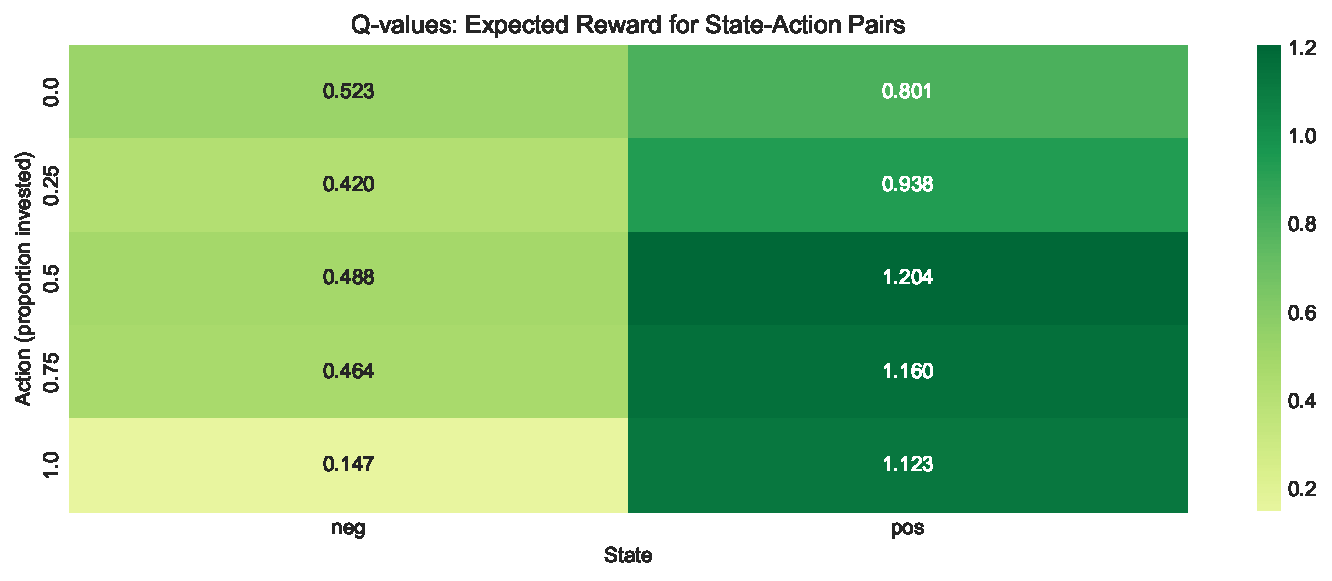
\includegraphics[width=0.7\linewidth]{files/5339e4b9396959054c44a6714f43952f.pdf}}
\label{fig-q_heatmap}
\end{figure}

\paragraph{Q-learning with market data}\label{sec_RLemp2}

The second application is based on the financial dataset. To reduce the dimensionality of the problem, we will assume that:

\begin{itemize}
\item only one feature (price-to-book ratio) captures the state of the environment. This feature is processed so that it has only a limited number of possible values;
\item actions take values over a discrete set consisting of three positions: +1 (buy the market), -1 (sell the market) and 0 (hold no risky positions);
\item only two assets are traded: those with fsym\_id equal to 3 and 4 - they both have 245 days of trading data.
\end{itemize}

The construction of the dataset is coded below.

\begin{verbatim}
# Get unique stock IDs to find appropriate assets
stock_counts = data_ml.groupby('fsym_id').size().reset_index(name='count')
print(f"Number of unique stocks: {len(stock_counts)}")
print(f"Stocks with most data points:")
print(stock_counts.nlargest(10, 'count'))

# Select two stocks with sufficient data
# We'll use the first two stocks with the most data points
top_stocks = stock_counts.nlargest(2, 'count')['fsym_id'].values
stock_1, stock_2 = top_stocks[0], top_stocks[1]
print(f"\nSelected stocks: {stock_1}, {stock_2}")
\end{verbatim}

\begin{verbatim}
Number of unique stocks: 846
Stocks with most data points:
      fsym_id  count
34   BV3N5V-R    266
47   BZPTB8-R    266
60   CHKL7S-R    266
68   CPCV0Y-R    266
73   CSMTMQ-R    266
79   CYBC69-R    266
84   D1LJ47-R    266
91   D68LVD-R    266
108  DJBQ39-R    266
128  F17SJ1-R    266

Selected stocks: BV3N5V-R, BZPTB8-R
\end{verbatim}

\begin{verbatim}
# Extract data for the two selected stocks
data_stock_1 = data_ml[data_ml['fsym_id'] == stock_1].copy()
data_stock_2 = data_ml[data_ml['fsym_id'] == stock_2].copy()

# Get common dates
common_dates = set(data_stock_1['date']).intersection(set(data_stock_2['date']))
data_stock_1 = data_stock_1[data_stock_1['date'].isin(common_dates)].sort_values('date')
data_stock_2 = data_stock_2[data_stock_2['date'].isin(common_dates)].sort_values('date')

print(f"Number of common time points: {len(common_dates)}")

# Extract returns and P/B ratios
return_1 = data_stock_1['R1M'].values
return_2 = data_stock_2['R1M'].values
pb_1 = data_stock_1['PB'].values
pb_2 = data_stock_2['PB'].values

# Random actions for each asset: -1, 0, or 1
n_obs = len(return_1)
action_1 = np.floor(np.random.uniform(0, 1, n_obs) * 3) - 1  # -1, 0, or 1
action_2 = np.floor(np.random.uniform(0, 1, n_obs) * 3) - 1

# Build the RL dataset
RL_data = pd.DataFrame({
    'return_1': return_1,
    'return_2': return_2,
    'pb_1': pb_1,
    'pb_2': pb_2,
    'action_1': action_1.astype(int),
    'action_2': action_2.astype(int)
})

# Unite actions into a single string
RL_data['action'] = RL_data['action_1'].astype(str) + ' ' + RL_data['action_2'].astype(str)

# Simplify states by rounding 5 * P/B ratio
RL_data['pb_1_disc'] = np.round(5 * RL_data['pb_1']).astype(int)
RL_data['pb_2_disc'] = np.round(5 * RL_data['pb_2']).astype(int)

# Unite states into a single string
RL_data['state'] = RL_data['pb_1_disc'].astype(str) + '.' + RL_data['pb_2_disc'].astype(str)

# Compute rewards: portfolio return
RL_data['reward'] = RL_data['action_1'] * RL_data['return_1'] + RL_data['action_2'] * RL_data['return_2']

# Infer next state
RL_data['new_state'] = RL_data['state'].shift(-1)

# Keep only relevant columns and remove last row (no next state)
RL_data = RL_data[['state', 'action', 'reward', 'new_state']].dropna()

print("\nFirst rows of the market data RL dataset:")
RL_data.head()
\end{verbatim}

\begin{verbatim}
Number of common time points: 266

First rows of the market data RL dataset:
\end{verbatim}

\bigskip\noindent
\begin{tabular}{p{\dimexpr 0.200\linewidth-2\tabcolsep}p{\dimexpr 0.200\linewidth-2\tabcolsep}p{\dimexpr 0.200\linewidth-2\tabcolsep}p{\dimexpr 0.200\linewidth-2\tabcolsep}p{\dimexpr 0.200\linewidth-2\tabcolsep}}
\toprule
 & state & action & reward & new\_state \\
\hline
0 & 1.4 & 1 -1 & -0.008839 & 1.4 \\
\hline
1 & 1.4 & 0 0 & 0.000000 & 1.4 \\
\hline
2 & 1.4 & 0 1 & 0.187156 & 1.4 \\
\hline
3 & 1.4 & 1 0 & 0.061398 & 1.4 \\
\hline
4 & 1.4 & 0 0 & 0.000000 & 1.4 \\
\hline
\bottomrule
\end{tabular}

\bigskip

Actions and states have to be merged to yield all possible combinations. To simplify the states, we round 5 times the price-to-book ratios.

We keep the same hyperparameters as in the previous example. Columns below stand for actions: the first (\textit{resp.} second) number notes the position in the first (\textit{resp.} second) asset. The rows correspond to states. The scaled P/B ratios are separated by a point (e.g., ``2.3'' means that the first (\textit{resp.} second) asset has a scaled P/B of 2 (\textit{resp.} 3).

\begin{verbatim}
# Get unique states and actions from the data
states_market = RL_data['state'].unique().tolist()
actions_market = RL_data['action'].unique().tolist()

print(f"Number of unique states: {len(states_market)}")
print(f"Number of unique actions: {len(actions_market)}")
print(f"Total state-action pairs: {len(states_market) * len(actions_market)}")

# Initialize Q-learning agent for market data
agent_market = QLearningAgent(
    states=states_market,
    actions=actions_market,
    alpha=0.1,
    gamma=0.7,
    epsilon=0.1
)

# Train the agent
agent_market.train_on_data(RL_data)

# Display the Q-table
print("\nQ-table (rounded to 3 decimals):")
q_table_market = agent_market.get_q_table().round(3)
print(q_table_market)

print("\nOptimal policy for some states:")
policy = agent_market.get_policy()
for state in list(policy.keys())[:5]:
    print(f"  State {state}: best action = {policy[state]}")
\end{verbatim}

\begin{verbatim}
Number of unique states: 18
Number of unique actions: 9
Total state-action pairs: 162

Q-table (rounded to 3 decimals):
      1 -1    0 0    0 1    1 0   -1 1   -1 0  -1 -1    1 1   0 -1
1.4 -0.015  0.010  0.039 -0.015 -0.041  0.034 -0.003  0.042 -0.049
1.5 -0.010  0.000  0.000 -0.004  0.000  0.000  0.000  0.000  0.000
2.4 -0.009  0.021  0.002  0.000 -0.007 -0.057  0.012  0.108 -0.006
3.4  0.003  0.006 -0.010 -0.001  0.000 -0.007  0.040 -0.018 -0.000
1.3 -0.019  0.002  0.018  0.019 -0.016  0.013 -0.010 -0.030 -0.016
1.2  0.000  0.000  0.000 -0.001  0.000  0.004 -0.002  0.000  0.000
1.1  0.004  0.000  0.000  0.000  0.022  0.000  0.000 -0.017  0.024
2.1 -0.002  0.001 -0.006  0.000 -0.007  0.000  0.013 -0.017  0.000
1.0  0.000  0.000  0.000  0.011  0.000  0.019  0.015 -0.017  0.010
0.0 -0.011  0.000  0.000  0.000 -0.021  0.000 -0.092 -0.022  0.000
2.2  0.000  0.000  0.000  0.005  0.000  0.000 -0.048  0.000  0.007
3.2  0.000  0.000  0.000  0.000  0.000 -0.018  0.005  0.029  0.000
3.3 -0.016  0.003  0.000  0.009 -0.002  0.008  0.011  0.009  0.009
2.3 -0.027  0.000  0.006 -0.005  0.009 -0.012  0.000  0.000 -0.010
4.4 -0.007  0.004  0.020  0.027 -0.004 -0.003  0.006 -0.019 -0.008
4.3  0.004  0.002  0.000  0.000  0.000  0.000  0.000  0.000  0.000
0.3  0.000  0.001 -0.027  0.000  0.000  0.000  0.000  0.067  0.000
0.4  0.000  0.000  0.000  0.000  0.009  0.000  0.000  0.000  0.000

Optimal policy for some states:
  State 1.4: best action = 1 1
  State 1.5: best action = 0 0
  State 2.4: best action = 1 1
  State 3.4: best action = -1 -1
  State 1.3: best action = 1 0
\end{verbatim}

The output shows that there are many combinations of states and actions that are not spanned by the data: basically, the $Q$ function has a zero and it is likely that the combination has not been explored. Some states seem to be more often represented, others, less. It is hard to make any sense of the recommendations. Some states are close but the outcomes related to them can be very different. Moreover, there is no coherence and no monotonicity in actions with respect to individual state values: low values of states can be associated to very different actions.

One reason why these conclusions do not appear trustworthy pertains to the data size. With only 200+ time points and many state-action pairs, this yields on average only a few data points to compute the $Q$ function. This could be improved by testing more random actions, but the limits of the sample size would eventually (rapidly) be reached anyway. This is left as an exercise (see below).

\paragraph{Visualization of Q-values for Market Data}

\begin{figure}[!htbp]
\centering
\begin{verbatim}
# Select most common states for visualization
state_counts = RL_data['state'].value_counts()
top_states = state_counts.head(8).index.tolist()

# Filter Q-table for visualization
q_subset = q_table_market.loc[top_states]

fig, ax = plt.subplots(figsize=(12, 6))
sns.heatmap(q_subset, annot=True, fmt='.3f', cmap='RdYlGn', center=0, ax=ax)
ax.set_xlabel('Action (position in asset 1, position in asset 2)')
ax.set_ylabel('State (scaled P/B of asset 1 . scaled P/B of asset 2)')
ax.set_title('Q-values for Most Common States in Market Data')
plt.tight_layout()
plt.show()
\end{verbatim}
\caption[]{Heatmap of Q-values for market data environment (truncated for readability).

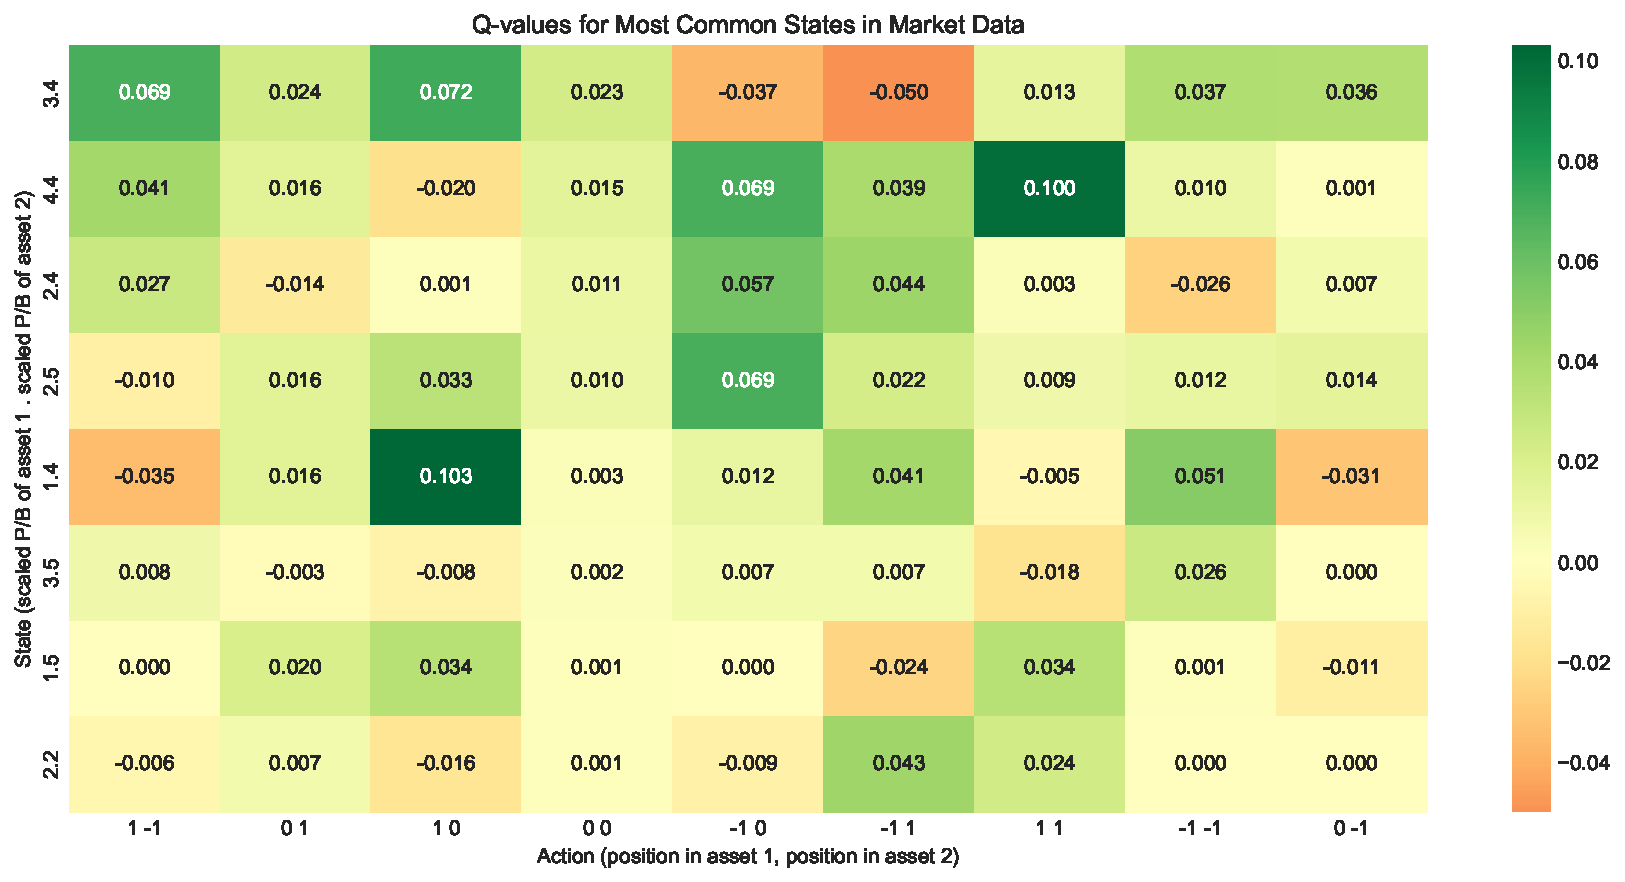
\includegraphics[width=0.7\linewidth]{files/78baaa7133b7a411a12679c7cb59b8b0.pdf}}
\label{fig-q_market_heatmap}
\end{figure}

\subsubsection{Modern RL Approaches: Deep Q-Networks}

The tabular Q-learning approach shown above suffers from the curse of dimensionality. Modern approaches use \textbf{function approximation} to represent the Q-function, typically with neural networks. This is the foundation of \textbf{Deep Q-Networks (DQN)}, which was popularized by DeepMind's work on playing Atari games.

Below, we provide a simple implementation of DQN using Keras for the same simulated environment. Keras 3 supports multiple backends including JAX, TensorFlow, and PyTorch. This demonstrates how neural networks can scale Q-learning to continuous or high-dimensional state spaces.

\begin{verbatim}
class DQNKeras:
        """
        A Deep Q-Network implemented with Keras.
        Compatible with JAX, TensorFlow, or PyTorch backends.
        """
        def __init__(self, state_dim, action_dim, hidden_dim=64, lr=0.001):
            # Build the Q-network
            inputs = keras.Input(shape=(state_dim,))
            x = layers.Dense(hidden_dim, activation='relu')(inputs)
            x = layers.Dense(hidden_dim, activation='relu')(x)
            outputs = layers.Dense(action_dim, activation='linear')(x)
            
            self.model = Model(inputs=inputs, outputs=outputs)
            self.model.compile(
                optimizer=optimizers.Adam(learning_rate=lr),
                loss='mse'
            )
            self.action_dim = action_dim
        
        def predict(self, state):
            """Predict Q-values for a state."""
            state = np.atleast_2d(state)
            return self.model.predict(state, verbose=0)
        
        def update(self, states, targets):
            """Update the network on a batch."""
            return self.model.train_on_batch(states, targets)
    
class DQNAgent:
        """
        Deep Q-Network agent with experience replay using Keras.
        """
        def __init__(self, state_dim, action_dim, lr=0.001, gamma=0.99, epsilon=0.1):
            self.state_dim = state_dim
            self.action_dim = action_dim
            self.gamma = gamma
            self.epsilon = epsilon
            
            self.network = DQNKeras(state_dim, action_dim, hidden_dim=64, lr=lr)
            
            # Experience replay buffer
            self.memory = []
            self.memory_size = 10000
        
        def choose_action(self, state):
            """Choose action using epsilon-greedy policy."""
            if np.random.random() < self.epsilon:
                return np.random.randint(self.action_dim)
            else:
                q_values = self.network.predict(state)
                return np.argmax(q_values[0])
        
        def store_experience(self, state, action, reward, next_state, done):
            """Store experience in replay buffer."""
            if len(self.memory) >= self.memory_size:
                self.memory.pop(0)
            self.memory.append((state, action, reward, next_state, done))
        
        def train(self, batch_size=32):
            """Train the network on a batch from the replay buffer."""
            if len(self.memory) < batch_size:
                return None
            
            # Sample batch
            indices = np.random.choice(len(self.memory), batch_size, replace=False)
            batch = [self.memory[i] for i in indices]
            
            states = np.array([b[0] for b in batch])
            actions = np.array([b[1] for b in batch])
            rewards = np.array([b[2] for b in batch])
            next_states = np.array([b[3] for b in batch])
            dones = np.array([b[4] for b in batch])
            
            # Compute targets using Bellman equation
            current_q = self.network.predict(states)
            next_q = self.network.predict(next_states)
            
            # Q-learning target: r + gamma * max(Q(s', a'))
            targets = current_q.copy()
            for i in range(batch_size):
                if dones[i]:
                    targets[i, actions[i]] = rewards[i]
                else:
                    targets[i, actions[i]] = rewards[i] + self.gamma * np.max(next_q[i])
            
            # Update network
            loss = self.network.update(states, targets)
            return loss
    
print("DQN agent class defined successfully.")
\end{verbatim}

\begin{verbatim}
Keras 3.12.0 available with backend: jax
DQN agent class defined successfully.
\end{verbatim}

\begin{verbatim}
if KERAS_AVAILABLE:
    # Train DQN on simulated AR(1) environment
    np.random.seed(42)
    
    # State: normalized return (continuous)
    # Actions: 0=0%, 1=25%, 2=50%, 3=75%, 4=100% invested
    action_values = [0.0, 0.25, 0.5, 0.75, 1.0]
    
    agent_dqn = DQNAgent(state_dim=1, action_dim=5, lr=0.001, gamma=0.7, epsilon=0.1)
    
    # Train on simulated data
    n_episodes = 100
    episode_length = 1000
    losses = []
    
    for episode in range(n_episodes):
        # Simulate returns
        returns_episode = simulate_ar1(episode_length, rho, a, sd)
        episode_loss = 0
        n_updates = 0
        
        for t in range(episode_length - 1):
            # State: current return (normalized)
            state = [returns_episode[t] / sd]  # Normalize
            
            # Choose action
            action_idx = agent_dqn.choose_action(state)
            action = action_values[action_idx]
            
            # Compute reward
            reward = returns_episode[t + 1] * action
            
            # Next state
            next_state = [returns_episode[t + 1] / sd]
            done = (t == episode_length - 2)
            
            # Store and train
            agent_dqn.store_experience(state, action_idx, reward, next_state, done)
            loss = agent_dqn.train(batch_size=64)
            if loss is not None:
                episode_loss += loss
                n_updates += 1
        
        avg_loss = episode_loss / max(n_updates, 1)
        losses.append(avg_loss)
        
        if (episode + 1) % 20 == 0:
            print(f"Episode {episode + 1}/{n_episodes}, Avg Loss: {avg_loss:.6f}")
    
    print("\nDQN training complete.")
\end{verbatim}

\begin{verbatim}
Episode 20/100, Avg Loss: 0.088640
Episode 40/100, Avg Loss: 0.087876
Episode 60/100, Avg Loss: 0.088382
Episode 80/100, Avg Loss: 0.089057
Episode 100/100, Avg Loss: 0.089003

DQN training complete.
\end{verbatim}

\begin{figure}[!htbp]
\centering
\begin{verbatim}
if KERAS_AVAILABLE:
    # Visualize the learned policy
    state_range = np.linspace(-3, 3, 100)
    q_values_all = []
    
    for s in state_range:
        q_vals = agent_dqn.network.predict([s]).flatten()
        q_values_all.append(q_vals)
    
    q_values_all = np.array(q_values_all)
    
    # Plot Q-values for each action
    fig, axes = plt.subplots(1, 2, figsize=(14, 5))
    
    # Q-values
    for i, label in enumerate(['0%', '25%', '50%', '75%', '100%']):
        axes[0].plot(state_range, q_values_all[:, i], label=f'{label} invested')
    axes[0].set_xlabel('State (normalized return)')
    axes[0].set_ylabel('Q-value')
    axes[0].set_title('Q-values by State and Action')
    axes[0].legend()
    axes[0].axvline(x=0, color='gray', linestyle='--', alpha=0.5)
    
    # Optimal action
    optimal_actions = np.argmax(q_values_all, axis=1)
    optimal_allocations = [action_values[a] for a in optimal_actions]
    
    axes[1].plot(state_range, optimal_allocations, 'b-', linewidth=2)
    axes[1].set_xlabel('State (normalized return)')
    axes[1].set_ylabel('Optimal Allocation')
    axes[1].set_title('Optimal Policy: Allocation vs State')
    axes[1].axvline(x=0, color='gray', linestyle='--', alpha=0.5)
    axes[1].set_ylim(-0.05, 1.05)
    
    plt.tight_layout()
    plt.show()
\end{verbatim}
\caption[]{Learned policy from DQN: optimal allocation as a function of the state (normalized return).

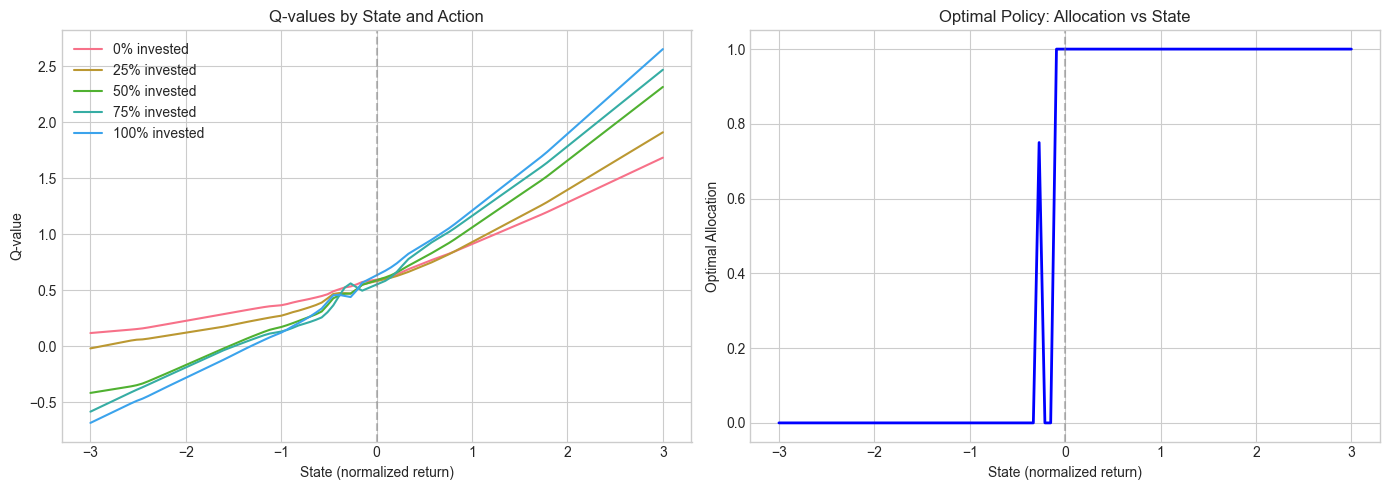
\includegraphics[width=0.7\linewidth]{files/58e57e9e6e19ef96444cb3f98197d659.png}}
\label{fig-dqn_policy}
\end{figure}

The DQN learns a policy that is consistent with the tabular Q-learning result: invest more when the previous return is positive (exploiting the positive autocorrelation) and invest less when the previous return is negative. The advantage of DQN is that it can handle continuous states without discretization, and it scales to much higher-dimensional problems.

\subsubsection{Concluding remarks}

Reinforcement learning has been applied to financial problems for a long time. Early contributions in the late 1990s include \cite{neuneier1996optimal}, \cite{moody1997optimization}, \cite{moody1998performance} and \cite{neuneier1998enhancing}. Since then, many researchers in the computer science field have sought to apply RL techniques to portfolio problems. The advent of massive datasets and the increase in dimensionality make it hard for RL tools to adapt well to very rich environments that are encountered in factor investing.

Recently, some approaches seek to adapt RL to continuous action spaces (\cite{wang2019continuous}, \cite{aboussalah2020continuous}) but not to high-dimensional state spaces. These spaces are those required in factor investing because all firms yield hundreds of data points characterizing their economic situation. In addition, applications of RL in financial frameworks have a particularity compared to many typical RL tasks: in financial markets, actions of agents have \textbf{no impact on the environment} (unless the agent is able to perform massive trades, which is rare and ill-advised because it pushes prices in the wrong direction). This lack of impact of actions may possibly mitigate the efficiency of traditional RL approaches.

Those are challenges that will need to be solved in order for RL to become competitive with alternative (supervised) methods. Nevertheless, the progressive (online-like) way RL works seems suitable for non-stationary environments: the algorithm slowly shifts paradigms as new data arrives. In stationary environments, it has been shown that RL manages to converge to optimal solutions (\cite{kong2019new}, \cite{chaouki2020deep}). Therefore, in non-stationary markets, RL could be a recourse to build dynamic predictions that adapt to changing macroeconomic conditions. More research needs to be carried out in this field on large dimensional datasets.

We end this chapter by underlining that reinforcement learning has also been used to estimate complex theoretical models (\cite{halperin2018market}, \cite{garcia2019continuous}). The research in the field is incredibly diversified and is orientated towards many directions. It is likely that captivating work will be published in the near future.

\subsubsection{Exercises}

\begin{enumerate}
\item Test what happens if the process for generating returns has a negative autocorrelation. What is the impact on the $Q$ function and the policy?
\item Keeping the same 2 assets as in Section~\ref{sec_RLemp2}, increase the size of RL\_data by testing \textbf{all possible action combinations} for each original data point. Re-run the $Q$-learning function and see what happens.
\item Implement SARSA (Equation \ref{eq-SARSAupdate}) and compare its performance with Q-learning on the simulated AR(1) environment.
\item Modify the DQN implementation to use \textbf{Double DQN} (separate networks for action selection and value estimation) and compare performance.
\item Implement a simple \textbf{policy gradient} method (REINFORCE) for the AR(1) environment using Keras and compare with Q-learning approaches.
\end{enumerate}

\subsubsection{Additional Topics: Stable-Baselines3 Integration}

For more sophisticated RL applications, the \textbf{Stable-Baselines3} library provides production-ready implementations of various RL algorithms (PPO, SAC, TD3, etc.). Below is an example of how to set up a custom financial environment compatible with the Gymnasium interface.

\begin{verbatim}
class SimplePortfolioEnv(gym.Env):
        """
        A simple portfolio environment for RL.
        
        State: normalized past return
        Action: proportion to invest in risky asset (continuous [0,1])
        Reward: portfolio return
        """
        metadata = {'render_modes': ['human']}
        
        def __init__(self, rho=0.8, a=0.048, sd=0.4, max_steps=252):
            super().__init__()
            
            self.rho = rho
            self.a = a
            self.sd = sd
            self.max_steps = max_steps
            
            # Continuous action space: allocation in [0, 1]
            self.action_space = spaces.Box(low=0, high=1, shape=(1,), dtype=np.float32)
            
            # Observation: normalized return
            self.observation_space = spaces.Box(low=-10, high=10, shape=(1,), dtype=np.float32)
            
            self.reset()
        
        def reset(self, seed=None, options=None):
            super().reset(seed=seed)
            self.current_return = self.a / (1 - self.rho)  # Unconditional mean
            self.step_count = 0
            obs = np.array([self.current_return / self.sd], dtype=np.float32)
            return obs, {}
        
        def step(self, action):
            allocation = float(action[0])
            
            # Generate next return (AR(1))
            epsilon = np.random.normal(0, self.sd)
            next_return = self.a + self.rho * self.current_return + epsilon
            
            # Portfolio return
            reward = allocation * next_return
            
            # Update state
            self.current_return = next_return
            self.step_count += 1
            
            # Check if done
            terminated = self.step_count >= self.max_steps
            truncated = False
            
            obs = np.array([self.current_return / self.sd], dtype=np.float32)
            
            return obs, reward, terminated, truncated, {}
    
# Test the environment
env = SimplePortfolioEnv()
obs, _ = env.reset()
print(f"Initial observation: {obs}")
    
# Take a few random steps
total_reward = 0
for _ in range(10):
        action = env.action_space.sample()
        obs, reward, terminated, truncated, info = env.step(action)
        total_reward += reward
        if terminated:
            break
    
print(f"After 10 steps, total reward: {total_reward:.4f}")
print("Environment is compatible with Stable-Baselines3!")
\end{verbatim}

\begin{verbatim}
Initial observation: [0.6]
After 10 steps, total reward: -0.9202
Environment is compatible with Stable-Baselines3!
\end{verbatim}

This environment can be used with Stable-Baselines3 algorithms:

\begin{verbatim}
from stable_baselines3 import PPO, SAC

# Using PPO (Proximal Policy Optimization)
model = PPO("MlpPolicy", env, verbose=1)
model.learn(total_timesteps=100000)

# Or using SAC (Soft Actor -Critic) for continuous actions
model = SAC("MlpPolicy", env, verbose=1)
model.learn(total_timesteps=100000)
\end{verbatim}

These modern algorithms handle continuous action spaces natively and include various improvements over basic Q-learning, such as entropy regularization, importance sampling, and policy clipping.

\section{Natural language processing for factor investing}

\subsection{Classical NLP for factor investing}

% 
% Version: 1.0.5
% Last updated: 2026-07-21
% Versioning scheme:
%   MAJOR: structural overhaul, renumbering of top-level sections, new Parts
%   MINOR: new section, new figure, new content batch, new vendor table column
%   PATCH: prose tweaks, citation additions, single-bib-entry fixes, typo fixes
% See `VERSIONING_ch20.md` in chapter folder for the change log.
% Provenance: this chapter is the first of five chapters in Part V of the
% 2nd edition, extracted from the monolithic Chapter_20_Draft19.md
% (v3.9.7, 48,526 words, archived in `_archive_monolithic_v3.9.7/`).
%

\subsubsection{Introduction}

The preceding chapters of this book have explored a wide array of machine learning tools for factor investing, from penalized regressions (Chapter 5) and tree-based models (Chapter 6) to neural networks (Chapter 7), reinforcement learning (Chapter 16), and genetic algorithms (Chapter 19). All of these methods operate on the same type of input: structured, numerical data organized into a matrix of firm characteristics. The book's standard dataset of 1,207 US stocks with 93 features (see Chapter 1) epitomizes this paradigm. Yet a vast reservoir of economically relevant information is encoded not in numbers but in words.

Corporate filings, earnings call transcripts, analyst reports, news articles, central bank communications, and social-media posts contain forward-looking statements, managerial tone, risk disclosures, and sentiment cues that are difficult (and often impossible) to capture through numerical characteristics alone. The field of \textit{natural language processing} (NLP) provides the tools to convert this unstructured text into quantitative signals suitable for factor models and portfolio construction.

The relevance of text for asset pricing is well established empirically. Earlier foundations were laid by \cite{antweiler2004internet}, who showed that the volume and disagreement of Internet stock message board posts predict next-day volatility and trading activity, and by \cite{das2007yahoo}, who classified Yahoo! Finance messages about 24 technology stocks and found that aggregate sentiment tracks intraday returns. Building on this foundation, \cite{tetlock2007giving} showed that the fraction of negative words in a Wall Street Journal column predicted next-day Dow Jones returns. \cite{loughran2011liability} demonstrated that generic sentiment dictionaries misclassify financial language and proposed a domain-specific lexicon that has since become the standard.

This chapter focuses on the \textit{classical} NLP toolkit that has driven text-based factor research for two decades, and that remains the right starting point for any production pipeline. We introduce text as a data class and survey the six source families that recur throughout Part V (Section 20.2), define the preprocessing and bag-of-words representations that every downstream method consumes (Section 20.3), develop the dictionary-based sentiment scoring that opened the field empirically (Section 20.4), introduce topic models for thematic factor discovery (Section 20.5), present named-entity recognition and event extraction for event-driven strategies (Section 20.6), and close with the two factor families that the classical toolkit has produced in mature, peer-reviewed form: disclosure-based factors (Section 20.7) and news and media-flow factors (Section 20.8). The remainder of the NLP toolkit (embeddings, transformers, large language models, and an end-to-end case study) is deferred to the following chapters.

NLP for equity markets is now a vast and rapidly growing literature: corpus surveys identify on the order of 1,000 or more papers since the late 2000s, with roughly 76\% appearing after 2021 alone \citep{lis2024investor}. Two structural axes organize the field. The first is a \textit{method curve} that runs from rule-based lexicons through classical machine learning and dense embeddings to BERT-style encoders and, finally, generative LLMs; \cite{mishev2020evaluation} provide the canonical benchmark spanning this entire arc, testing approximately 30 sentiment models on financial text and finding that transformers dominate accuracy while sacrificing transparency. The second is a \textit{source curve}: early studies focused on news articles and message boards because they are short and syntactically simple, while longer and more specialized documents such as earnings-call transcripts and 10-K filings only became tractable once transformer-scale encoders arrived around 2019-2020.
Two caveats are in order. First, the book's standard \texttt{mlfi\_us\_data} panel is numerical only: it does not contain textual data, in keeping with the design of the dataset described in Chapter 1. Shipping a raw text corpus alongside this book would be problematic on two counts. Legally, although individual corporate filings, earnings-call transcripts, and news articles are public, their bulk redistribution sits in a grey zone: publishers and transcript vendors retain copyright on the typeset record, and SEC filings are public but not licence-free when repackaged at scale. Practically, assembling a research-grade corpus of millions of filings, transcripts, and news items is an engineering project (storage, deduplication, OCR for older filings, ticker mapping, point-in-time alignment) that is well outside the scope of a methods textbook. To mitigate both concerns we ship a \textit{sentiment-derived} companion dataset rather than the raw text itself: for the 437 largest US stocks in \texttt{mlfi\_us\_data} we processed the full available history of quarterly earnings-call transcripts and recorded the per-call sentiment scores produced by each of the model families introduced across Part V (classical dictionaries, contextual encoders, and an LLM-based scorer), split into prepared-remarks, Q\&A-management, and Q\&A-analyst buckets. Distributing scores rather than text sidesteps the licensing question and shrinks the artifact from terabytes to a single panel CSV. The empirical tables of Chapter 21 and the case study of Chapter 24 read from this companion panel directly; the methodology subsections of the present chapter use much shorter illustrative samples (a single Coca-Cola Q1 2026 transcript excerpt and a handful of stylised sentences) when the pedagogical point is the technique itself rather than its cross-sectional performance. Second, NLP is a vast and fast-moving field. We do not attempt encyclopedic coverage; instead, we focus on the methods most directly relevant to equity factor investing and refer the interested reader to \cite{jurafsky2024speech} for a comprehensive treatment of the broader NLP landscape, and to the finance-specific survey of \cite{xing2018natural}, which catalogues the text sources (news, filings, message boards, social media), modeling families (lexicon, statistical, deep learning), and applications (return and volatility forecasting, event studies) that underpin the literature Part V draws on.

\textbf{A note on notation in this chapter.} Several equations in this chapter use letters that double as both NLP and asset-pricing indices. We highlight the local redefinitions to avoid confusion. In Equation (20.7), $n$ indexes word positions within a document (not assets) and $N_d$ is the document length. In Equation (20.8), $t$ indexes corpus tokens and $T$ the corpus length (not calendar time). The symbol $\alpha$ appears in two distinct roles: a Dirichlet concentration vector in Equation (20.7) and a portfolio intercept in Equation (20.13); context disambiguates in each case. We retain these letter choices because they are standard in the NLP literature, but we flag them here so that the cross-reference to Chapter 1's notation is unambiguous.

\subsubsection{Text as a data class}

Text differs from the structured numerical features of Chapters 2 through 19 in three ways that drive every design choice that follows. It is \textit{high-dimensional}: a typical 10-K contains 50,000 to 150,000 tokens (the atomic word or word-piece units a text is broken into, defined precisely in Section 20.3.1) drawn from a vocabulary of tens of thousands of distinct types, so any representation must compress aggressively before reaching a tractable feature space. It is \textit{semantic}: identical numbers (``revenue grew 5\%'') carry very different signals depending on the surrounding context (guidance versus historical, prepared remarks versus Q\&A, peer comparison versus stand-alone), so encodings that ignore surrounding context (the classical bag-of-words representation defined in Section 20.3.2, which simply counts how often each word appears) throw away information that the contextual encoders of Chapter 22 (transformer models whose representation of each word depends on the entire sentence) preserve. And it is \textit{irregularly timed}: filings appear on quarterly schedules with embargoed release windows, earnings calls are clustered in two-week reporting waves, news arrives continuously with intra-day spikes, and social-media posts arrive in bursts driven by events; this temporal heterogeneity dictates how text-derived features should be aligned to the monthly factor frequency of the book's dataset.

These three properties motivate a \textit{data-class} view of text. Rather than treating ``text'' as a single source, we partition the universe of financial text into six classes that differ along the dimensions that matter for factor investing: producer (firm, analyst, journalist, regulator, retail investor), publication frequency, regulatory status, signal-to-noise ratio, coverage breadth, and typical document length. Each class supports a distinct set of metrics and a distinct set of factor strategies, and each has accumulated its own peer-reviewed empirical literature.
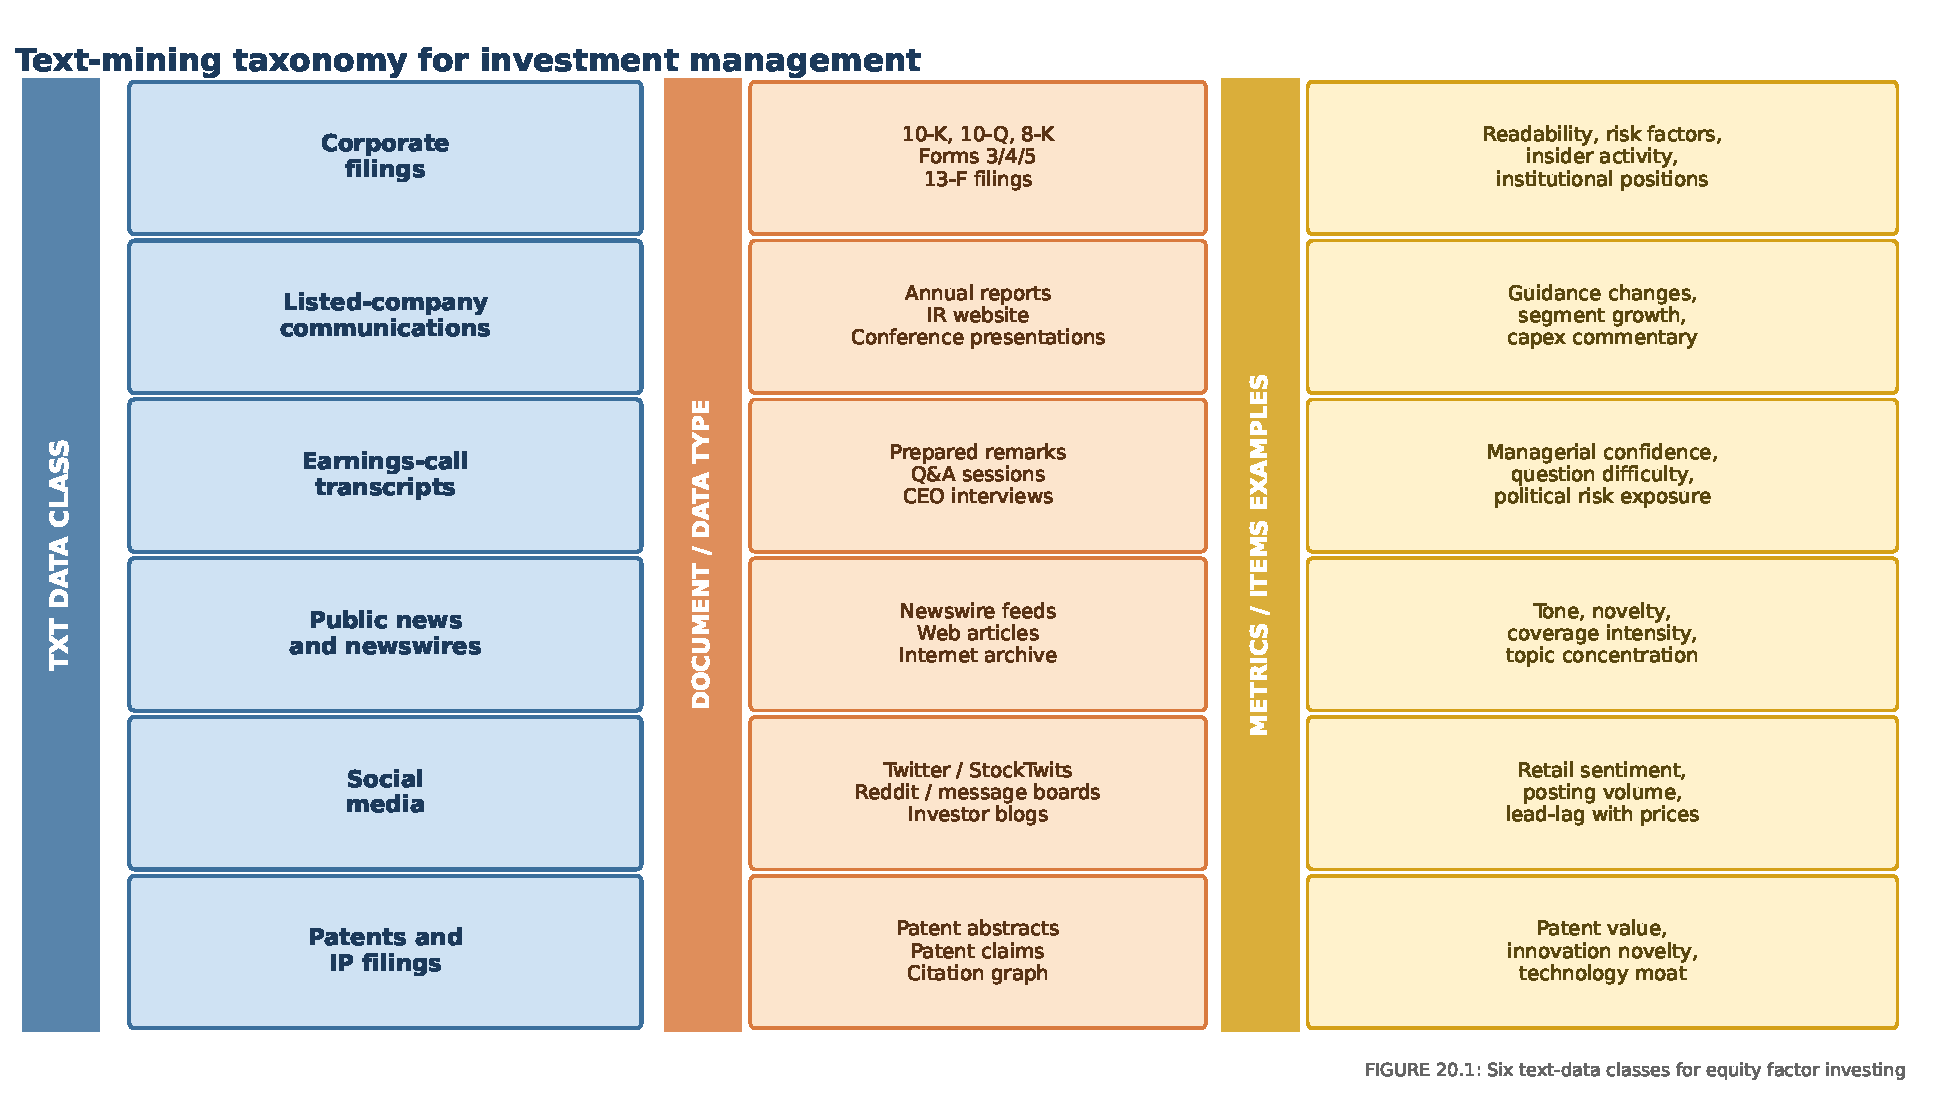
\includegraphics[width=0.7\linewidth]{files/figure_20_1_taxonomy-b9a4f75ffab7a7164fe7d0585f2b1dd1.pdf}

FIGURE 20.1 organizes the six text-data classes along three axes (data class, document or data type, metrics or items examples) following the standard practitioner taxonomy used in industry research. We now describe each row in turn, summarizing what the class is, who produces it, what use cases it enables, and which published evidence anchors it in the empirical literature.

\paragraph{Corporate filings (10-K, 10-Q, 8-K, Forms 3/4/5, 13-F)}

Filings submitted to the U.S. Securities and Exchange Commission are the most regulated text class in the financial system. The annual 10-K and quarterly 10-Q reports contain audited financial statements wrapped in extensive textual discussion, including the Management's Discussion and Analysis (MD\&A), risk factors, and forward-looking statements. The 8-K reports material events as they occur; Forms 3, 4, and 5 disclose insider transactions; and 13-F filings reveal quarterly institutional positions above the reporting threshold. These documents are long (typically 100 to 300 pages for a 10-K), uniformly formatted, infrequent (quarterly to annual), and legally vetted, which makes them high-signal but slow-moving. The classical evidence on filings runs through \cite{loughran2011liability}, whose finance-specific sentiment dictionary corrects the systematic misclassification of generic lexicons on legal and accounting prose; \cite{li2008annual}, who showed that 10-K readability (Fog index) predicts earnings persistence; \cite{cohen2020lazy}, who documented the Lazy Prices anomaly whereby year-over-year textual changes in 10-Ks generate a long-short return of roughly 23.5\% per annum; \cite{bushee2018linguistic}, who decompose linguistic complexity into obfuscation and information components; \cite{hoberg2016text}, who build text-based industry classifications from 10-K product descriptions; \cite{campbell2014information}, who quantify the information content of mandatory risk factor disclosures; and \cite{lopezlira2023risk}, who extracts risk factors directly from 10-K text and prices them in the cross-section.

\paragraph{Listed-company communications (annual reports, IR websites, conference presentations)}

Beyond mandatory SEC filings, listed companies maintain a parallel stream of voluntary communications: glossy annual reports, investor-relations website content, sustainability reports, capital-markets-day decks, and conference presentations to sell-side analysts. These materials are less constrained by accounting standards but governed by Regulation Fair Disclosure, which prohibits selective release of material information. They are useful for extracting forward-looking commentary that is downplayed or absent in SEC filings: total addressable market estimates, net sales by geography and product segment, segment-level growth narratives, capex guidance, and product-pipeline disclosures. The empirical evidence here is thinner than for SEC filings but growing: \cite{sautner2023firm} construct firm-level climate change exposure measures by combining earnings calls with IR communications, and \cite{webersinke2022climatebert} pretrain ClimateBERT on a large corpus of corporate sustainability reports and use it to score voluntary climate disclosures across firms.

\paragraph{Earnings call transcripts}

Quarterly earnings conference calls are perhaps the richest single-source text class for equity factor investing. Each call has two parts with very different information content: prepared remarks (10 to 30 minutes), in which management reads a scripted account of the quarter, and the Q\&A session (typically 30 to 60 minutes), in which sell-side analysts question executives in real time. Transcripts are publicly available with a delay measured in hours and cover essentially every US-listed company that holds a quarterly earnings call. \cite{larcker2012detecting} identified linguistic markers of deceptive language by executives who subsequently restated earnings; \cite{hassan2019politicalrisk} extracted firm-level political risk scores from transcripts that load on lobbying activity and predict the cross-section of returns; \cite{sautner2023firm} measured climate exposure at the firm level; \cite{kim2024transcripts} used a generative LLM to distil firm-level risk assessments from earnings-call transcripts that explain return volatility and firms' risk-mitigating actions better than dictionary-based measures; \cite{hafez2021transcripts} showed that document sentiment, event sentiment, and disclosure transparency are three largely orthogonal signals extractable from the same transcript; \cite{zhao2018alpha} demonstrated that the Q\&A portion of the call carries substantially more cross-sectional alpha than the prepared remarks; and \cite{yang2020html} introduced HTML, the hierarchical transformer architecture that has since become standard for long-form transcript modeling.

\paragraph{Public news and newswires}

News is the most-studied text class in the literature and the dominant data source in every method era surveyed by \cite{mishev2020evaluation}. It is heterogeneous in publisher (Wall Street Journal, Reuters, Dow Jones, Bloomberg, regional newspapers, financial blogs), frequency (intra-day to daily), and coverage (broad market commentary versus firm-specific news). The canonical empirical results start with \cite{tetlock2007giving}, who showed that the negative-word share in a single daily WSJ column predicts next-day Dow returns; \cite{tetlock2008more}, who generalized the finding to firm-specific news; \cite{antweiler2004internet} on Internet message-board volumes; \cite{engelberg2011causal}, who isolated the \textit{causal} effect of local newspaper coverage on local trading via weather-driven distribution disruptions; \cite{hillert2014media}, whose interaction of past returns with press coverage drives the momentum factor; \cite{heston2017news}, who built a news-tone factor not subsumed by price momentum; \cite{garcia2013sentiment} on the recession-dependence of news sentiment effects; \cite{calomiris2019news} on novelty-weighted sentiment in a 51-country sample; \cite{manela2017news}, who construct the NVIX disaster-concerns index from front-page articles since 1890; and \cite{ke2019predicting}, who push the out-of-sample (OOS) predictive frontier with their SESTM (Sentiment Extraction via Screening and Topic Modeling) supervised text learner over Dow Jones news. Two early methodological studies anchor the historical foundation of the literature for this data class: \cite{devitt2007sentiment}, working with cohesion-based analysis of financial news, were among the first to demonstrate rigorously that textual tone carries price-relevant information beyond prices themselves, and \cite{schumaker2012evaluating}, in one of the canonical early studies in \textit{Decision Support Systems}, showed that lexicon-based sentiment over news articles produces reliable predictive signals for stock returns.

\paragraph{Social media (Twitter/X, StockTwits, Reddit, message boards)}

Social media is the youngest and noisiest text class in the taxonomy, characterised by very short documents (Twitter's 280-character limit), heavy slang and emoji usage, severe class imbalance (most posts are neutral chatter), and intermittent retail-sentiment regimes that can shift abruptly during specific events (GameStop 2021, AMC 2021, COVID 2020). Despite these challenges, peer-reviewed evidence on its information content is robust: \cite{bollen2011twitter} reported aggregate Twitter mood as a leading indicator of DJIA moves; \cite{chen2014wisdom} used Seeking Alpha posts to predict next-quarter earnings; \cite{bartov2018twitter} showed that pre-announcement Twitter sentiment predicts both earnings surprises and announcement-day returns, particularly for low-coverage names; \cite{xu2018stock} released the StockNet dataset (88 stocks, two years of tweets and prices) that has become a standard NLP benchmark; \cite{zheludev2014when} provide a negative-control finding that the lead-lag effect of Twitter on the S\&P 500 is detectable for high-volume cashtags but absent at the aggregate index level; \cite{sawhney2020deep} introduced graph-attention models that combine tweet content with inter-company correlation graphs; and \cite{albladi2025twitter} survey the post-transformer state of the art across the broader Twitter sentiment literature.

\paragraph{Patents and intellectual property filings}

The final class in our taxonomy, patents, is the least developed in the equity factor investing literature but is included here because it sits at the intersection of two robust signals: corporate R\&D effort (a quality factor proxy) and innovation novelty (an asset-pricing factor in its own right). Patent abstracts describe what the invention does, patent claims define what is legally protected, and the patent citation graph captures intellectual debt and influence. Useful firm-level metrics derived from patent text include the patent-family size (how broadly an invention is protected internationally), expiration timelines (which affect future cash flows), novelty keywords (which proxy for breakthrough innovation), the count of citing patents (an empirical proxy for technology-moat strength), and concept exposure to specific technology themes. The flagship paper in this area, \cite{kogan2017technological}, measures patent value from text and shows that text-derived novelty predicts future cash flows and stock returns; although outside the dominant news and transcript literature of this chapter, the methodology is a natural extension of the techniques developed in Sections 20.3 through 20.7 and an open avenue for factor researchers working at the intersection of IP economics and asset pricing.

\subsubsection{Text as data: preprocessing and representation}

\paragraph{From raw text to clean tokens}

Before any quantitative analysis can begin, raw text must be transformed into a structured representation. This preprocessing pipeline is the foundation of all NLP methods, classical and modern alike, and its quality directly affects downstream performance. We outline the standard steps below.

\textbf{Tokenization} is the process of splitting a string of text into individual units called \textit{tokens}. In the simplest case, tokens are words separated by whitespace, but financial text often requires more nuanced treatment. Consider the string \texttt{"Q3 2023 EPS beat by \$0.12"}: a naive whitespace tokenizer would treat \texttt{"\$0.12"} as a single token, while a more sophisticated tokenizer might separate the currency symbol from the number. The \texttt{nltk} library provides several tokenizers suited to different use cases.

\begin{verbatim}
import nltk
nltk.download('punkt_tab', quiet=True)
sentence = "EPS of $0.86 increased 18% year-over-year, helped by 3% currency tailwinds."
print(nltk.word_tokenize(sentence))      # NLTK splits punctuation from numbers
\end{verbatim}

\begin{verbatim}
['EPS', 'of', '$', '0.86', 'increased', '18', '%', 'year-over-year', ',', 'helped', 'by', '3', '%', 'currency', 'tailwinds', '.']
\end{verbatim}

The tokenizer isolates the dollar sign and the percent sign as their own tokens, which is useful for a downstream rule that wants to identify currency or magnitude expressions, but it also splits \texttt{"18"} from \texttt{"\%"}, so any pipeline that wants the original \texttt{"18\%"} magnitude back must reassemble adjacent tokens (or use a custom regular-expression tokenizer).

\textbf{Stop-word removal} eliminates high-frequency words that carry little semantic content: ``the,'' ``is,'' ``and,'' ``of.'' Removing these words reduces the dimensionality of the representation and focuses subsequent analysis on content-bearing terms. However, in financial text, some seemingly generic words can carry meaning (e.g., ``will'' in forward-looking statements), so the choice of stop-word list requires domain judgment.

\begin{verbatim}
from nltk.corpus import stopwords
nltk.download('stopwords', quiet=True)
stop = set(stopwords.words('english'))
sentence = "We are continuing to judiciously manage our balance sheet as we await a court decision."
tokens = [t for t in nltk.word_tokenize(sentence.lower()) if t.isalpha()]
print([t for t in tokens if t not in stop])
\end{verbatim}

\begin{verbatim}
['continuing', 'judiciously', 'manage', 'balance', 'sheet', 'await', 'court', 'decision']
\end{verbatim}

Eight content-bearing tokens survive out of seventeen original tokens. The pronouns (``we,'' ``our''), auxiliaries (``are,'' ``to,'' ``as''), and the article (``a'') are dropped; ``balance sheet'' and ``court decision'' survive as the substantive concepts.

\textbf{Stemming and lemmatization} reduce words to their root forms. Stemming applies crude suffix-stripping rules (``running'' becomes ``run,'' ``consolidation'' becomes ``consolid''), while lemmatization uses morphological analysis to produce valid dictionary forms (``better'' becomes ``good,'' ``are'' becomes ``be''). For financial applications, lemmatization is generally preferred because it preserves interpretability: ``diversified'' and ``diversification'' both reduce to ``diversify'' rather than the truncated stem ``diversif.''

\begin{verbatim}
from nltk.stem import WordNetLemmatizer, PorterStemmer
nltk.download('wordnet', quiet=True)
lem, stem = WordNetLemmatizer(), PorterStemmer()
words = ['consumers', 'monitored', 'preferring', 'flavors', 'evenings', 'better']
print('lemmas:', [lem.lemmatize(w) for w in words])
print('stems :', [stem.stem(w) for w in words])
\end{verbatim}

\begin{verbatim}
lemmas: ['consumer', 'monitored', 'preferring', 'flavor', 'evening', 'better']
stems : ['consum', 'monitor', 'prefer', 'flavor', 'even', 'better']
\end{verbatim}

Lemmatization keeps real dictionary words but only normalises plurals (\texttt{consumers \rightarrow consumer}) unless we pass the right part-of-speech tag for verbs; the Porter stemmer is more aggressive and collapses inflections but produces non-words such as \texttt{consum} and \texttt{even}. Neither method handles \texttt{better \rightarrow good} without a richer morphological resource (NLTK's WordNet lemmatizer with \texttt{pos='a'} would).

\textbf{Handling financial jargon.} Domain-specific vocabulary poses particular challenges. Ticker symbols (AAPL, MSFT), financial abbreviations (EPS, EBITDA, P/E), and compound terms (free-cash-flow, mark-to-market) require custom tokenization rules. Negation handling is especially important: ``not profitable'' should not be treated as two independent tokens in a bag-of-words model. We discuss this further in Section 20.4.3.

\begin{verbatim}
import re
sentence = "Free cash flow was approximately $1.8 billion year-over-year, with no signs of slowing demand."
protect = {'free cash flow': 'free_cash_flow',           # compound term
           'year-over-year': 'year_over_year',           # hyphenated metric
           'no signs of slowing': 'NEG_slowing'}         # negation scope
for src, tgt in protect.items():
    sentence = re.sub(src, tgt, sentence, flags=re.IGNORECASE)
print(nltk.word_tokenize(sentence))
\end{verbatim}

\begin{verbatim}
['free_cash_flow', 'was', 'approximately', '$', '1.8', 'billion', 'year_over_year', ',', 'with', 'NEG_slowing', 'demand', '.']
\end{verbatim}

The substitution pass collapses multi-word financial terms into single tokens before the generic tokenizer runs, preserving them as atomic units downstream. The negation cue is rewritten with a \texttt{NEG\_} prefix on the modified word, so that a bag-of-words sentiment scorer that does not understand syntax still sees \texttt{NEG\_slowing} as a distinct feature rather than positive \texttt{slowing} plus a discarded \texttt{no}.

We illustrate the preprocessing pipeline on six real excerpts taken from the Coca-Cola Q1 2026 earnings call transcript (Coca-Cola, henceforth referenced by its NYSE ticker KO). In practice, the corpus would consist of thousands of 10-K filing excerpts, earnings call paragraphs, or news articles; here a single call already shows the variety of language a sentiment pipeline must cope with.

\begin{verbatim}
import nltk                                          # NLP toolkit
from nltk.corpus import stopwords
from nltk.stem import WordNetLemmatizer
nltk.download('punkt_tab', quiet=True)
nltk.download('stopwords', quiet=True)
nltk.download('wordnet', quiet=True)

documents = [                                        # KO Q1 2026 excerpts
    "We delivered strong first quarter results despite a complex external environment.",
    "Many consumers remain under pressure due to persistent inflation and greater macroeconomic uncertainty.",
    "We harnessed the power of our brands to deliver three percent volume growth across all segments.",
    "Management expects organic revenue growth on track with our full year guidance.",
    "The softness in price mix was attributed to Easter timing and unfavorable category mix from packaged water.",
    "Innovation contributed strongly to revenue growth with Coca Cola Cherry and Diet Coke Cherry powering volume.",
]

lemmatizer = WordNetLemmatizer()
stop_words = set(stopwords.words('english'))

def preprocess(text):
    """Tokenize, lowercase, remove stop words, lemmatize."""
    tokens = nltk.word_tokenize(text.lower())        # Tokenize and lowercase
    tokens = [t for t in tokens if t.isalpha()]       # Keep alphabetic tokens only
    tokens = [t for t in tokens if t not in stop_words]  # Remove stop words
    tokens = [lemmatizer.lemmatize(t) for t in tokens]   # Lemmatize
    return tokens

processed = [preprocess(doc) for doc in documents]
for i, tokens in enumerate(processed):
    print(f"Doc {i}: {tokens}")
\end{verbatim}

\begin{verbatim}
Doc 0: ['delivered', 'strong', 'first', 'quarter', 'result', 'despite', 'complex', 'external', 'environment']
Doc 1: ['many', 'consumer', 'remain', 'pressure', 'due', 'persistent', 'inflation', 'greater', 'macroeconomic', 'uncertainty']
Doc 2: ['harnessed', 'power', 'brand', 'deliver', 'three', 'percent', 'volume', 'growth', 'across', 'segment']
Doc 3: ['management', 'expects', 'organic', 'revenue', 'growth', 'track', 'full', 'year', 'guidance']
Doc 4: ['softness', 'price', 'mix', 'attributed', 'easter', 'timing', 'unfavorable', 'category', 'mix', 'packaged', 'water']
Doc 5: ['innovation', 'contributed', 'strongly', 'revenue', 'growth', 'coca', 'cola', 'cherry', 'diet', 'coke', 'cherry', 'powering', 'volume']
\end{verbatim}

The preprocessing reduces each sentence to its content-bearing lemmas. Notice that ``consumers'' becomes ``consumer,'' ``results'' becomes ``result,'' and common words like ``the,'' ``a,'' ``by'' are removed. The plural ``segments'' is normalised to ``segment,'' and the proper nouns ``Coca,'' ``Cola,'' ``Cherry,'' and ``Coke'' survive as lowercase tokens that a downstream entity-recognition pass (Section 20.6) would tag back as brand names. The resulting token lists are the raw material for the bag-of-words representation introduced in the next subsection.

\paragraph{Bag-of-words and term frequency}

The simplest numerical representation of a text document is the \textit{bag-of-words} (BoW) model: a vector whose length equals the vocabulary size $V$ and whose $k$-th entry counts how many times word $k$ appears in the document. This representation discards word order entirely, treating ``the dog bit the man'' and ``the man bit the dog'' identically.

Let $d$ denote a document and $\mathcal{V} = \{w_1, \ldots, w_V\}$ the vocabulary. The raw term-frequency vector is:

\begin{equation}
\text{tf}(w_k, d) = \frac{\text{count}(w_k, d)}{\sum_{j=1}^{V} \text{count}(w_j, d)}
\tag{20.1}
\end{equation}

where $\text{count}(w_k, d)$ is the number of occurrences of word $w_k$ in document $d$.

Given a corpus of $D$ documents, the \textit{document-term matrix} (DTM) $\mathbf{X} \in \mathbb{R}^{D \times V}$ stores the term frequencies (or raw counts) for all documents. Each row is a document, each column is a word. This matrix is typically very sparse, because any single document uses only a small fraction of the total vocabulary.

Raw term frequency overweights common words. The \textit{term frequency-inverse document frequency} (TF-IDF) weighting addresses this by down-weighting terms that appear in many documents:

\begin{equation}
\text{tf-idf}(w_k, d) = \text{tf}(w_k, d) \times \log \frac{D}{\text{df}(w_k)}
\tag{20.2}
\end{equation}

where $\text{df}(w_k)$ is the number of documents containing word $w_k$. The logarithmic term penalizes words that appear across most documents (e.g., ``company,'' ``quarter'') while boosting words that are distinctive to a few documents (e.g., ``goodwill impairment,'' ``FDA approval''). TF-IDF is arguably the most widely used text representation in applied finance, owing to its simplicity and effectiveness.

We now construct the TF-IDF matrix from the same six KO Q1 2026 excerpts preprocessed above.

\begin{verbatim}
from sklearn.feature_extraction.text import TfidfVectorizer

vectorizer = TfidfVectorizer(
    tokenizer=preprocess,                            # custom preprocessor from §20.3.1
    token_pattern=None,                              # disable default pattern
    max_features=30)                                 # limit vocabulary for display
tfidf_matrix = vectorizer.fit_transform(documents)
feature_names = vectorizer.get_feature_names_out()

# The full 6 x 30 matrix is very sparse: print only the top 4 highest-weighted
# terms per document, which is the empirically useful view of TF-IDF.
for i, row in enumerate(tfidf_matrix.toarray()):
    pairs = sorted(zip(feature_names, row), key=lambda x: -x[1])
    top4  = [f'{t} ({w:.2f})' for t, w in pairs[:4] if w > 0]
    print(f'Doc {i}: ' + ', '.join(top4))
\end{verbatim}

\begin{verbatim}
Doc 0: complex (0.41), delivered (0.41), despite (0.41), environment (0.41)
Doc 1: consumer (0.45), due (0.45), greater (0.45), inflation (0.45)
Doc 2: across (0.44), brand (0.44), deliver (0.44), harnessed (0.44)
Doc 3: expects (0.49), full (0.49), guidance (0.49), revenue (0.40)
Doc 4: mix (0.76), attributed (0.38), category (0.38), easter (0.38)
Doc 5: cherry (0.64), coca (0.32), contributed (0.32), diet (0.32)
\end{verbatim}

The full 6 by 30 TF-IDF matrix is extremely sparse, since each document uses only a small fraction of the vocabulary; the per-document top-4 view above is the empirically useful summary. The highest-weighted terms are those that are both frequent within a document and rare across the corpus. Doc 4 illustrates the construction cleanly: ``mix'' appears twice in that single document and nowhere else in the corpus, so it dominates the row with a weight of 0.76. Doc 5 is similar for ``cherry'', which appears twice in Doc 5 alone. The macroeconomic vocabulary of Doc 1 (``consumer'', ``inflation'', ``greater'', ``due'') and the forward-looking vocabulary of Doc 3 (``expects'', ``full'', ``guidance'') split cleanly along the prepared-remarks-versus-outlook axis that the chapter exploits throughout.

This representation, while simple, already captures meaningful structure. Documents about cash flows (Doc 2, Doc 4) share the terms ``cash'' and ``flow,'' while documents about losses (Doc 1) and earnings beats (Doc 5) are clearly separated. The challenge, of course, is that bag-of-words ignores word order and context entirely, a limitation we address in the sections that follow.

\subsubsection{Sentiment analysis with dictionaries}

\paragraph{The lexicon approach}

The most direct way to extract economic meaning from text is \textit{sentiment analysis}: classifying the tone of a document as positive, negative, or neutral. The simplest and most widely used approach in finance relies on pre-compiled \textit{sentiment dictionaries} (also called lexicons): curated lists of words labeled with their emotional or evaluative polarity.

Early work in computational linguistics used general-purpose lexicons such as the Harvard General Inquirer (GI), which classifies English words into psychological categories including positive and negative tone. \cite{loughran2011liability} showed that general-purpose lexicons perform poorly on financial text. Almost three-quarters of the words classified as ``negative'' by the Harvard GI are not negative in a financial context. The word ``tax,'' for instance, is labeled negative by the GI, yet it carries no evaluative tone in an earnings report. Similarly, ``liability,'' ``cost,'' and ``capital'' are flagged as negative despite being neutral financial terminology.

The \textbf{Loughran-McDonald (LM) dictionary} was specifically constructed for financial documents. The authors analyzed 10-K filings from 1994 to 2008 and identified six sentiment categories: \textit{negative}, \textit{positive}, \textit{uncertainty}, \textit{litigious}, \textit{strong modal}, and \textit{weak modal}. The negative word list (containing terms such as ``loss,'' ``impairment,'' ``decline,'' ``adverse,'' ``default'') has become the de facto standard for financial sentiment analysis. Subsequent studies have largely confirmed that domain-specific dictionaries outperform generic ones for financial text; the survey by \cite{kearney2014textual} provides a thorough review of these findings.

Given a dictionary with positive word set $\mathcal{P}$ and negative word set $\mathcal{N}$, the simplest sentiment score for a document $d$ is the \textit{net tone}:

\begin{equation}
\text{Tone}(d) = \frac{\#(d \cap \mathcal{P}) - \#(d \cap \mathcal{N})}{\#(d \cap \mathcal{P}) + \#(d \cap \mathcal{N})}
\tag{20.3}
\end{equation}

where $\#(d \cap \mathcal{P})$ counts the number of words in $d$ that belong to the positive list. This score ranges from -1 (entirely negative) to +1 (entirely positive). Alternative normalizations divide by total word count rather than the sum of sentiment words, but Equation (20.3) is the most common in the literature. \cite{jegadeesh2013word} showed that giving every LM-listed word equal weight in this formula is suboptimal, because some terms carry much stronger return-predictive content than others. They proposed a market-based term-weighting scheme that estimates each word's informativeness from its association with stock returns around 10-K filing dates, and reported that this data-driven weighting materially improves the out-of-sample predictive power of the tone score relative to the uniform weighting implicit in Equation (20.3).

We demonstrate the Loughran-McDonald approach using six sentences in the style of (and partly drawn from) the KO Q1 2026 earnings call already introduced in Section 20.3.1. In practice, researchers download the LM dictionary from the authors' website and apply it to large corpora of filings or news articles.

\begin{verbatim}
import numpy as np

# Loughran-McDonald word lists (abbreviated for illustration)
lm_positive = {
    'achieve', 'advancement', 'benefit', 'creative', 'efficient', 'enhance',
    'excellent', 'favorable', 'gain', 'great', 'improve', 'improvement',
    'innovation', 'opportunity', 'outstanding', 'positive', 'profitability',
    'progress', 'strength', 'strong', 'succeed', 'success', 'superior'
}
lm_negative = {
    'adverse', 'against', 'closure', 'decline', 'default', 'deficit',
    'deterioration', 'downturn', 'failure', 'impairment', 'inability',
    'litigation', 'loss', 'losses', 'negative', 'penalty', 'restructuring',
    'risk', 'terminate', 'threat', 'unfavorable', 'volatility', 'weakness'
}

sample_texts = [                                     # KO-flavored excerpts
    "Revenue growth was strong driven by innovation across our beverage portfolio.",
    "The softness in price mix was attributed to unfavorable category mix and constrained production capacity.",
    "Operating losses did not materialize, and margins held firm.",
    "Free cash flow improved and management sees favorable conditions for the remainder of the year.",
    "Adverse macroeconomic conditions and persistent inflation pose a risk to near-term consumer demand.",
    "The firm achieved outstanding results with superior margin expansion in North America.",
]
\end{verbatim}

\begin{verbatim}
def lm_sentiment(text, pos_words, neg_words):
    """Compute Loughran-McDonald net tone for a text."""
    tokens = set(text.lower().split())               # Simple whitespace tokenizer
    n_pos = len(tokens & pos_words)                  # Count positive matches
    n_neg = len(tokens & neg_words)                  # Count negative matches
    denom = n_pos + n_neg
    if denom == 0:
        return 0.0
    return (n_pos - n_neg) / denom                   # Net tone in [-1, 1]

scores = [lm_sentiment(t, lm_positive, lm_negative) for t in sample_texts]
for i, (text, score) in enumerate(zip(sample_texts, scores)):
    label = "Positive" if score > 0 else ("Negative" if score < 0 else "Neutral")
    print(f"Doc {i} ({label:>8s}, tone={score:+.2f}): {text[:60]}...")
\end{verbatim}

\begin{verbatim}
Doc 0 (Positive, tone=+1.00): Revenue growth was strong driven by innovation across our...
Doc 1 (Negative, tone=-1.00): The softness in price mix was attributed to unfavorable cat...
Doc 2 (Negative, tone=-1.00): Operating losses did not materialize, and margins held firm...
Doc 3 (Positive, tone=+1.00): Free cash flow improved and management sees favorable condi...
Doc 4 (Negative, tone=-1.00): Adverse macroeconomic conditions and persistent inflation p...
Doc 5 (Positive, tone=+1.00): The firm achieved outstanding results with superior margin ...
\end{verbatim}

The dictionary correctly identifies the dominant tone in most cases. Doc 0, 3, and 5 are scored as strongly positive, while Doc 1, 4 are strongly negative. However, Doc 2 illustrates the negation problem: ``operating losses did not materialize, and margins held firm'' is a positive statement, yet the dictionary scores it as -1.00 because ``losses'' is counted as a negative word while the negation ``did not materialize'' is ignored entirely. The dictionary cannot read the difference between ``losses occurred'' and ``losses did not materialize'' because it sees only a bag of words.

\begin{verbatim}
import matplotlib.pyplot as plt

fig, ax = plt.subplots(figsize=(8, 4))
colors = ['#2ecc71' if s > 0 else '#e74c3c' if s < 0 else '#95a5a6'
          for s in scores]
ax.barh(range(len(scores)), scores, color=colors)
ax.set_yticks(range(len(scores)))
ax.set_yticklabels([f'Doc {i}' for i in range(len(scores))])
ax.set_xlabel('Loughran-McDonald Net Tone')
ax.set_title('Dictionary-Based Sentiment Scores')
ax.axvline(x=0, color='black', linewidth=0.5)
plt.tight_layout()
plt.show()
\end{verbatim}

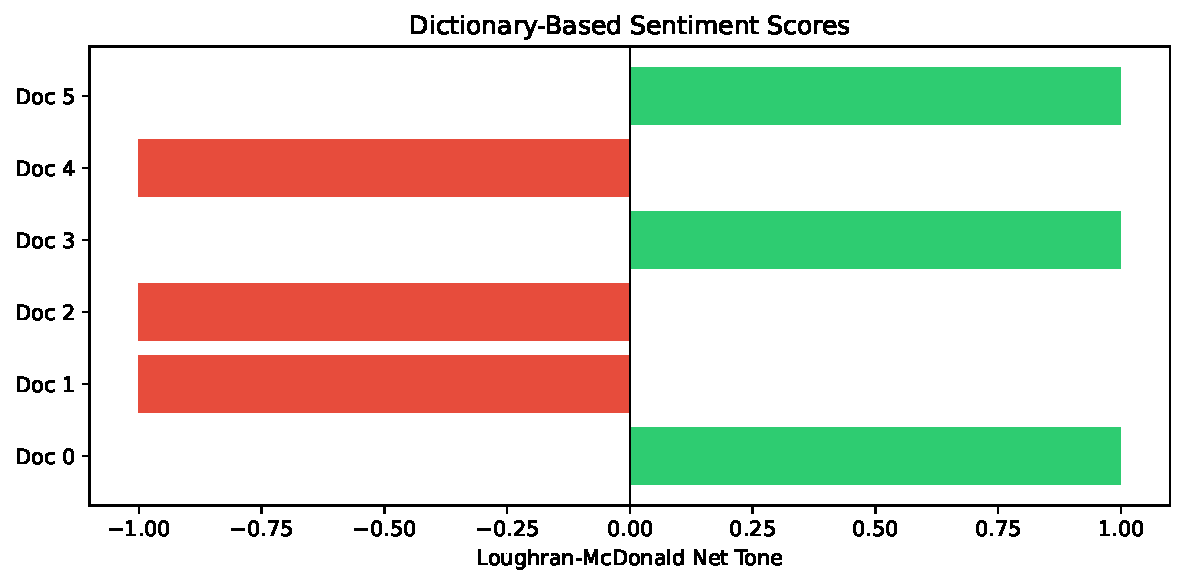
\includegraphics[width=0.7\linewidth]{files/figure_20_2_lm_score-b86dd1881505c7ad3da996bd7c706f84.pdf}

FIGURE 20.2 (panel a): dictionary-based sentiment scores for six KO-style sentences. Positive tone is shown in green, negative in red. Doc 2 illustrates the negation problem: a positive statement (``losses did not materialize, margins held firm'') receives a strongly negative score because the dictionary sees ``losses'' but cannot read ``did not materialize.''

The visualization in FIGURE 20.2 (panel a) makes the limitations of the dictionary approach immediately apparent. While the method works well for straightforward sentences, it systematically misclassifies negated statements. In Chapter 22, we will see that transformer-based models handle negation naturally through contextual representations.

\paragraph{From sentiment scores to factor signals}

The seminal application of textual sentiment to asset pricing is \cite{tetlock2007giving}, who studied the ``Abreast of the Market'' column in the Wall Street Journal. Using the Harvard GI to measure the fraction of negative words, Tetlock found that high media pessimism predicted downward pressure on market prices, followed by a reversion to fundamentals. Crucially, the effect was concentrated in small stocks with high individual investor ownership, consistent with a behavioral explanation in which noise traders overreact to negative tone.

This finding opened a productive line of research. \cite{tetlock2008more} extended the analysis to firm-level news and showed that the fraction of negative words in stories about individual firms predicted lower subsequent earnings, suggesting that journalists incorporate fundamentally relevant information. \cite{loughran2011liability} refined the measurement using their domain-specific dictionary and confirmed that negative tone in 10-K filings predicts higher post-filing return volatility, lower earnings, and wider bid-ask spreads. \cite{engelberg2011causal} pushed the literature a step further on causal identification: they used weather-driven disruptions to local newspaper delivery as an instrument and showed that local press coverage of S\&P 500 earnings announcements roughly doubles local trading activity, providing direct evidence that the media is not merely reporting prices but shaping them. \cite{hillert2014media} then connected sentiment to a classical anomaly by showing that firms with high media coverage exhibit substantially stronger momentum returns, with the effect largest for glamour stocks followed by many journalists, suggesting that press attention amplifies the behavioural frictions that sustain cross-sectional momentum.

To construct a news-tone factor for the cross-section, one typically proceeds as follows:

\begin{enumerate}
\item For each firm $n$ at time $t$, collect all relevant text documents (news articles, filings, transcripts) published during the period $(t -1, t]$.
\item Compute a sentiment score for each document using Equation (20.3) or a variant.
\item Aggregate across documents, possibly weighting by recency or source prominence, to obtain a firm-level sentiment signal $s_{t,n}$.
\item Use $s_{t,n}$ as a cross-sectional factor alongside the traditional characteristics from Chapter 1.
\end{enumerate}

To make the factor scale-invariant across periods we standardize the score cross-sectionally each rebalancing date,

\begin{equation}
z_{t,n} = \frac{s_{t,n} - \mu_t}{\sigma_t}, \quad \mu_t = \frac{1}{N_t}\sum_{n=1}^{N_t} s_{t,n}, \quad \sigma_t^2 = \frac{1}{N_t}\sum_{n=1}^{N_t} (s_{t,n} - \mu_t)^2
\tag{20.4}
\end{equation}

where the cross-section at date $t$ has $N_t$ firms. The portfolio implementation that we use throughout this chapter is the equal-weighted long-short \textit{decile spread},

\begin{equation}
r^{\text{LS}}_{t \to t+h} = \frac{1}{|\mathcal{D}_t^{10}|}\sum_{n \in \mathcal{D}_t^{10}} r_{t \to t+h, n} - \frac{1}{|\mathcal{D}_t^{1}|}\sum_{n \in \mathcal{D}_t^{1}} r_{t \to t+h, n}
\tag{20.5}
\end{equation}

with $\mathcal{D}_t^{10}$ and $\mathcal{D}_t^{1}$ the top and bottom deciles of $z_{t,n}$, and $r_{t \to t+h, n}$ the $h$-period total return on firm $n$. The cross-sectional information coefficient at horizon $h$, which we report extensively in the case study of Chapter 24, is the Spearman rank correlation between the standardized signal and the forward return computed within each cross-section and then averaged across dates,

\begin{equation}
\text{IC}(h) = \frac{1}{T}\sum_{t=1}^{T} \rho^{\text{Spearman}}\!\left(\{z_{t,n}\}_{n=1}^{N_t},\, \{r_{t \to t+h, n}\}_{n=1}^{N_t}\right).
\tag{20.6}
\end{equation}

Equations (20.4) through (20.6) supply the language we need to compare sentiment methods quantitatively: an information coefficient and a decile-spread Sharpe are the two summary statistics that the empirical tables of Chapter 21 and the case study of Chapter 24 are organized around.

The aggregation step is important and non-trivial. \cite{calomiris2019news} showed that \textit{novelty-weighted} sentiment, which down-weights language that merely repeats prior disclosures, is more informative for predicting returns than raw sentiment. The intuition is simple: a 10-K filing that repeats last year's risk factors verbatim contains less new information than one with substantially revised language.

The choice of aggregation window is equally consequential. \cite{hafez2012short} constructed several variants of a firm-level sentiment index from a commercial firm-level news sentiment dataset on a universe of 4,144 US stocks over 2000 to 2011, comparing absolute (net positive minus negative news count) and relative (positive share of total) measures across 1-day, 7-day, and 90-day rolling windows. They found that the 90-day window dominates: it smooths transient noise and captures the slower-moving component of sentiment that is most strongly associated with future returns. Using their preferred event-level score with a 90-day window, the average 3-day return spread between firms with positive and negative sentiment changes reaches 1.39\%, with most of the divergence occurring on the day the news is released. A long-short strategy built on this signal generates information ratios of 2 to 3 and a daily hit ratio close to 60\% before transaction costs. These figures should be read with the usual caveats (in-sample tuning, look-ahead in the universe construction, and gross-of-cost performance), but they illustrate a robust pattern: properly aggregated firm-level sentiment carries information beyond the contemporaneous return. An early explicit demonstration of this came from \cite{zhang2010trading}, who combined blog and news sentiment from a broad online corpus and showed that the resulting aggregate signals could be converted into profitable daily trading strategies across a large equity universe; their results were noisy at the individual-stock level but robust in aggregate, reinforcing the case for the cross-sectional sorting approach described above.

\paragraph{Limitations of dictionary methods}

Dictionary-based sentiment analysis is transparent, fast, and reproducible. It is also fundamentally limited by what we might call \textit{context blindness}. A dictionary treats each word independently, ignoring the syntactic and semantic structure of the sentence.

The most frequently cited limitation is \textbf{negation}. The sentence ``The company did not experience any significant losses'' is objectively positive, yet a dictionary approach that counts ``losses'' as negative and ignores ``not'' will assign a negative score. Various heuristic fixes exist (e.g., flipping the polarity of sentiment words that follow a negation cue within a fixed window), but they are fragile and incomplete.

\textbf{Intensifiers and diminishers} pose a related problem. ``Slightly disappointing'' and ``extremely disappointing'' carry very different magnitudes, but a dictionary assigns both the same polarity. Similarly, \textbf{conditional and hypothetical language} is common in financial text: ``If revenue were to decline, the company might need to restructure'' expresses a possibility, not a fact, yet a dictionary would count ``decline'' and ``restructure'' as negative.

\textbf{Sarcasm and implicit sentiment} are rare in formal financial documents but appear in social media and analyst commentary. A tweet reading ``Great job losing another billion dollars'' is clearly negative, but a dictionary would score ``great'' as positive.

Finally, \textbf{domain drift} is a practical concern. Language evolves, and the connotations of words change over time. A dictionary compiled from 1990s filings may not accurately capture sentiment in 2020s filings that discuss ``pandemic,'' ``supply chain disruptions,'' or ``generative AI.'' This static nature is a fundamental limitation that motivates the data-driven approaches of Chapters 21 through 23. \cite{lis2024investor} provides a useful perspective on how much of this gap has actually been closed: reviewing 71 empirical studies of investor sentiment in asset pricing models published between 2000 and 2021, the author documents that more complex sentiment measures do not reliably translate into better return prediction, and that survey-based, lexicon-based, and transformer-based signals often sit within overlapping error bars once implementation frictions are accounted for. The implication is not that modern methods are useless, but that the marginal gain per unit of modelling effort is smaller than the headlines of individual papers suggest.

A concrete out-of-sample replication of the central \cite{loughran2011liability} claim is available on a single large-cap name from the case-study corpus, KO. We score the prepared-remarks bucket of 68 KO earnings calls covering October 2006 through February 2026 with four sentiment methods (Harvard General Inquirer, the pre-LM baseline used by \cite{tetlock2007giving}; the LM dictionary; VADER, the rule-based lexicon of \cite{hutto2014vader}; and FinBERT, included here as a contextual-encoder benchmark that anticipates Chapter 22), and regress the resulting per-call score on the five-day post-call cumulative abnormal return (CAR) computed against the S\&P 500 ETF (SPY).

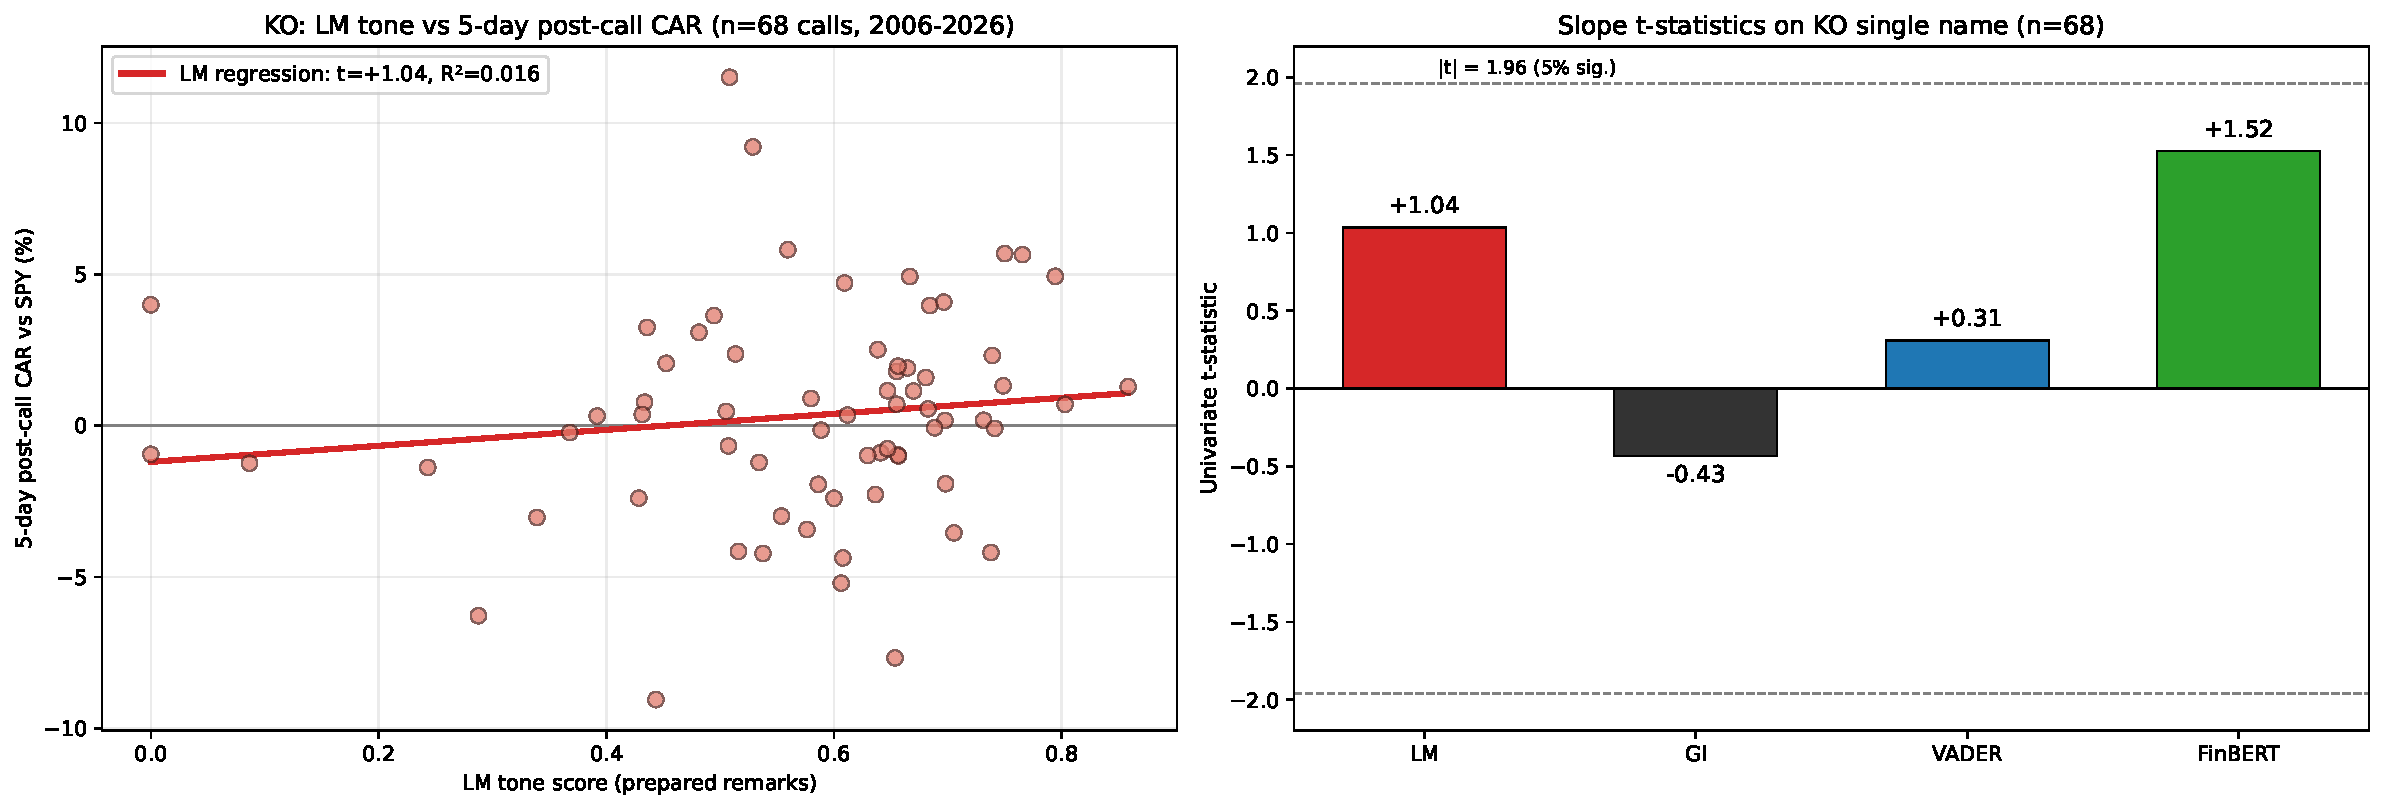
\includegraphics[width=0.7\linewidth]{files/figure_20_2b_ko_lm_r-8f34f57fa12d5e7bd12da50466e4057a.pdf}

Panel (b) of FIGURE 20.2 (KO single-name replication): the left sub-panel shows the scatter of KO five-day post-call CAR against the prepared-remarks LM tone, with the OLS regression line and its t-statistic. The right panel reports the slope t-statistics of the same regression for all four methods. On this single-name sample (n=68), LM achieves a univariate t-statistic of +1.04 with R\textsuperscript{2}=0.016, ahead of GI at -0.43 and VADER at +0.31. FinBERT, the only contextual-encoder method in the comparison, leads at t=+1.52 with R\textsuperscript{2}=0.034. None of these four single-name slopes is statistically significant at the 5\% level (|t|\textless 1.96), which is exactly the point: at a single large-cap name there is simply too little variation across 68 calls for any sentiment method to clear conventional significance, regardless of how sophisticated the model is. What the figure does illustrate is the \textit{qualitative} hierarchy that recurs at scale: LM outranks GI on the sign of the slope (consistent with the \cite{loughran2011liability} thesis that finance-domain dictionaries beat generic ones), and FinBERT in turn outranks LM (consistent with the contextual-encoder lift documented in Chapter 22).

\subsubsection{Topic modeling}

\paragraph{Latent Dirichlet Allocation}

While sentiment analysis reduces text to a single dimension (positive vs. negative), many financial applications require a richer representation that captures \textit{what} the text is about, not just its tone. \textit{Topic models} provide such a representation by discovering latent thematic structure in a corpus.

The most widely used topic model is \textbf{Latent Dirichlet Allocation} (LDA), introduced by \cite{blei2003latent}. The generative story behind LDA is elegant:

\begin{enumerate}
\item Each document is a mixture of $J$ latent topics, with mixing proportions $\boldsymbol{\theta}_d \sim \text{Dir}(\boldsymbol{\alpha})$.
\item Each topic $j$ is a distribution over the vocabulary, $\boldsymbol{\phi}_j \sim \text{Dir}(\boldsymbol{\beta})$.
\item For each word position in document $d$:

\begin{itemize}
\item Draw a topic assignment $z \sim \text{Multinomial}(\boldsymbol{\theta}_d)$.
\item Draw a word $w \sim \text{Multinomial}(\boldsymbol{\phi}_z)$.
\end{itemize}
\end{enumerate}

The Dirichlet priors $\boldsymbol{\alpha}$ and $\boldsymbol{\beta}$ control the sparsity of the topic mixtures and word distributions, respectively. A small $\alpha$ encourages documents to concentrate on a few topics; a small $\beta$ encourages topics to concentrate on a few words.

Formally, the joint distribution of a corpus of $D$ documents, given hyperparameters $\boldsymbol{\alpha}$ and $\boldsymbol{\beta}$, factorizes as

\begin{equation}
p(\mathbf{w}, \mathbf{z}, \boldsymbol{\theta}, \boldsymbol{\phi} \mid \boldsymbol{\alpha}, \boldsymbol{\beta}) = \prod_{j=1}^{J} p(\boldsymbol{\phi}_j \mid \boldsymbol{\beta}) \prod_{d=1}^{D} p(\boldsymbol{\theta}_d \mid \boldsymbol{\alpha}) \prod_{n=1}^{N_d} p(z_{d,n} \mid \boldsymbol{\theta}_d)\, p(w_{d,n} \mid \boldsymbol{\phi}_{z_{d,n}})
\tag{20.7}
\end{equation}

where $N_d$ is the length of document $d$ and $w_{d,n}, z_{d,n}$ are the $n$-th word and its latent topic assignment. Posterior inference targets the marginal $p(\mathbf{z} \mid \mathbf{w}, \boldsymbol{\alpha}, \boldsymbol{\beta})$, which has no closed form; in practice we estimate it by collapsed Gibbs sampling or variational Bayes. The key output for financial applications is the document-topic matrix $\boldsymbol{\Theta} \in \mathbb{R}^{D \times J}$, where $\theta_{d,j}$ represents the proportion of document $d$ that belongs to topic $j$. These topic proportions can serve directly as features in a factor model.

\paragraph{Financial applications}

Topic models have found several applications in equity investing. We highlight two prominent examples.

\textbf{Risk theme discovery.} \cite{israelsen2014does} applied LDA to the risk-factor sections (Item 1A) of 10-K filings and discovered interpretable risk themes such as ``litigation risk,'' ``regulatory risk,'' ``commodity price risk,'' and ``technology risk.'' Firms with high exposure to specific risk topics exhibited different return patterns, suggesting that topic proportions capture economically meaningful variation in firm-level risk that is not fully captured by traditional factors.

\textbf{Text-derived factors beyond Fama-French.} \cite{lopezlira2023risk} used topic models on news articles to construct text-based factors and showed that these factors span a significant portion of the cross-sectional variation in returns. The key insight is that topics capture latent themes (e.g., ``energy crisis,'' ``trade war,'' ``pandemic recovery'') that cut across traditional sector and style classifications.

The number of topics $J$ is a hyperparameter that must be chosen by the researcher. Common choices range from 10 to 50, depending on the granularity desired. Model selection criteria such as perplexity and topic coherence scores (\cite{roder2015exploring} survey the space of coherence measures) provide quantitative guidance, but human inspection of the top words per topic remains essential.

To make this concrete, we fit an LDA model to a small corpus of financial news headlines. In a production setting, the corpus would be much larger (thousands of articles per month), and the number of topics would be tuned using coherence metrics.

\begin{verbatim}
from sklearn.decomposition import LatentDirichletAllocation
from sklearn.feature_extraction.text import CountVectorizer

headlines = [
    "Federal Reserve raises interest rates by 25 basis points",
    "Oil prices surge amid Middle East tensions",
    "Tech stocks rally on strong earnings from Apple and Microsoft",
    "GDP growth slows as consumer spending weakens",
    "Central bank signals pause in monetary tightening cycle",
    "Crude oil futures fall on rising US production",
    "NASDAQ hits record high driven by AI chip demand",
    "Unemployment claims rise signaling labor market cooling",
    "European Central Bank holds rates steady citing inflation concerns",
    "Semiconductor stocks jump after strong guidance from NVIDIA",
    "Housing starts decline as mortgage rates reach 20-year high",
    "Gold prices rise as investors seek safe haven assets",
    "Retail sales disappoint raising recession fears",
    "Natural gas prices drop on mild winter forecasts",
    "Bond yields fall as markets price in rate cuts",
]

np.random.seed(42)
count_vec = CountVectorizer(
    stop_words='english',                            # Remove English stop words
    max_features=50                                  # Limit vocabulary size
)
dtm = count_vec.fit_transform(headlines)
\end{verbatim}

\begin{verbatim}
lda = LatentDirichletAllocation(
    n_components=3,                                  # Number of topics
    random_state=42,
    max_iter=20
)
topic_proportions = lda.fit_transform(dtm)

vocab = count_vec.get_feature_names_out()
for j in range(3):
    top_idx = lda.components_[j].argsort()[-6:][::-1]
    top_words = [vocab[i] for i in top_idx]
    print(f"Topic {j}: {', '.join(top_words)}")
\end{verbatim}

\begin{verbatim}
Topic 0: prices, rise, stocks, strong, haven, investors
Topic 1: oil, bank, central, european, holds, inflation
Topic 2: rates, fall, high, housing, decline, 20
\end{verbatim}

The topics are only partially interpretable, which is itself the lesson of running LDA on a corpus this small. Topic 2 is the cleanest: it groups the rate-and-macro headlines (the Fed hike, the GDP slowdown, housing starts, retail sales, and bond yields all load on it most heavily). Topic 1 collects energy and central-bank vocabulary (oil, crude, and the European Central Bank), and Topic 0 gathers an equities-and-safe-haven cluster (stocks, strong guidance, gold, and safe-haven demand). The separation is imperfect, with several headlines splitting their mass across topics, because fifteen short headlines give the model too little co-occurrence evidence to carve clean themes; the same procedure on tens of thousands of documents produces the sharp, stable topics that the technique is known for. We visualize the topic proportions for each headline in FIGURE 20.3.

\begin{verbatim}
fig, ax = plt.subplots(figsize=(10, 6))
im = ax.imshow(topic_proportions, aspect='auto', cmap='YlOrRd')
ax.set_yticks(range(len(headlines)))
ax.set_yticklabels([h[:50] + '...' if len(h) > 50 else h
                     for h in headlines], fontsize=8)
ax.set_xticks(range(3))
ax.set_xticklabels(['Equities/Haven', 'Energy/CB', 'Rates/Housing'])
ax.set_xlabel('Topic')
plt.colorbar(im, ax=ax, label='Topic proportion')
ax.set_title('LDA Topic Proportions for Financial Headlines')
plt.tight_layout()
plt.show()
\end{verbatim}

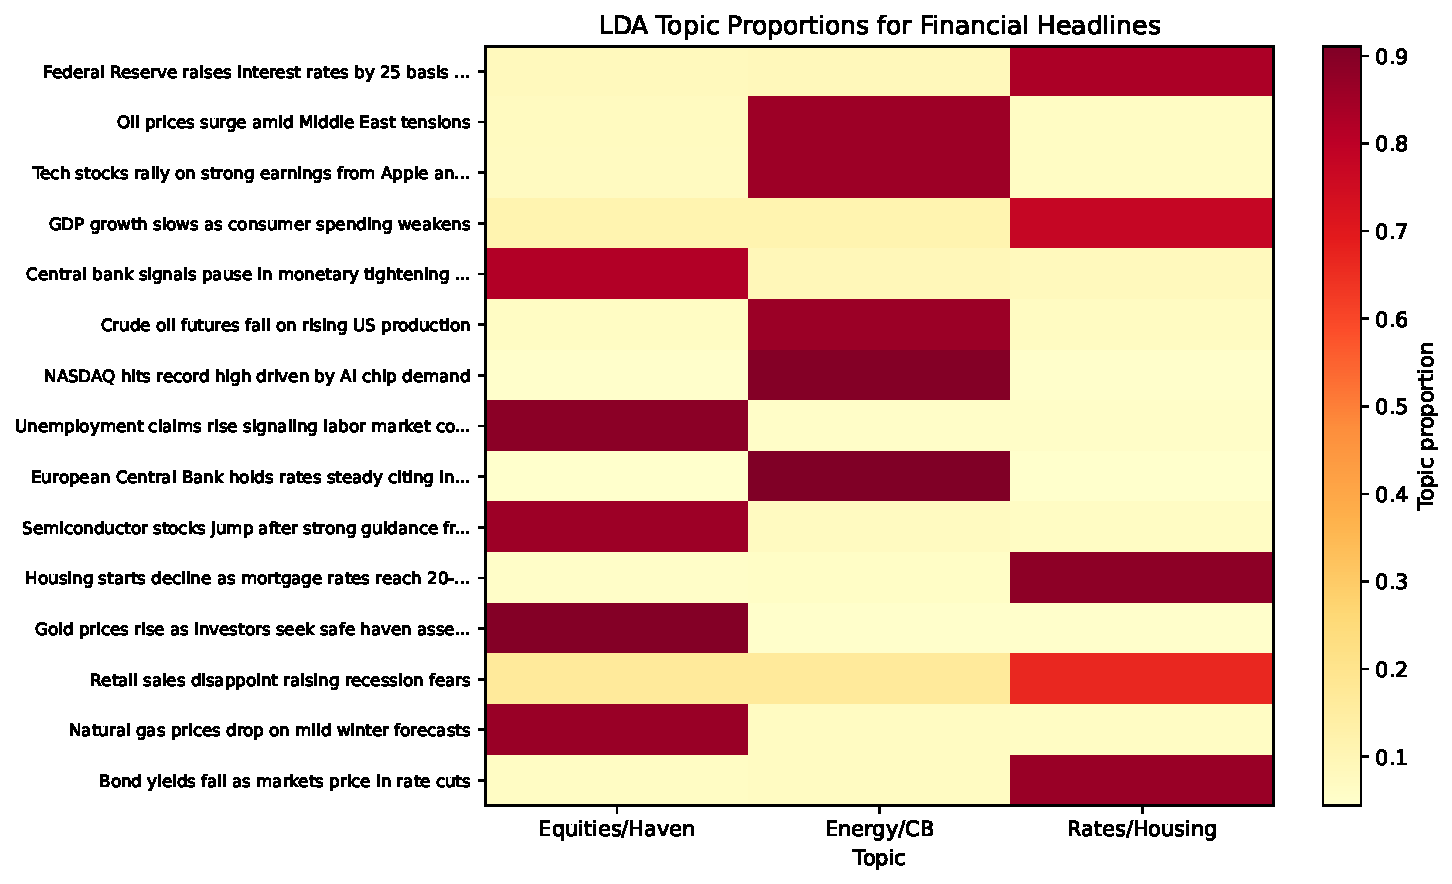
\includegraphics[width=0.7\linewidth]{files/figure_20_3_lda_heat-e9a6882d26eb6734a43933822ad956c3.pdf}

LDA topic proportions for 15 financial headlines. Each row shows the estimated mixture of three topics for one headline. The three columns correspond to the equities-and-safe-haven, energy-and-central-bank, and rates-and-housing clusters identified above.

The heatmap in FIGURE 20.3 shows how each headline distributes its mass across the three topics. The rate-and-macro headlines load most heavily on Topic 2, as expected: ``Federal Reserve raises interest rates'', ``Housing starts decline as mortgage rates reach 20-year high'', and ``Bond yields fall as markets price in rate cuts'' all peak there. The energy headlines (``Oil prices surge'', ``Crude oil futures fall'') concentrate on Topic 1, and the equities headlines (``Gold prices rise as investors seek safe haven assets'', ``Semiconductor stocks jump'') on Topic 0, though several headlines spread their proportions fairly evenly, a direct visual signal of the weak topic separation that a fifteen-document corpus produces.

\paragraph{Extensions}

Two extensions of standard LDA deserve mention. \textbf{Dynamic topic models} \citep{blei2006dynamic} allow topic distributions to evolve over time, which is natural for financial applications where the salience of themes (e.g., ``pandemic,'' ``inflation,'' ``AI'') changes across market regimes. \textbf{Structural topic models} (STM) introduced by \cite{roberts2014structural} incorporate document-level metadata (e.g., publication date, firm sector, filing type) as covariates that influence the topic proportions. This allows the researcher to ask questions such as ``Do firms in the energy sector discuss regulatory risk more than firms in technology?'' while controlling for other observable characteristics. A further extension is to couple topic assignments with sentiment scoring rather than treating the two as independent pipelines. \cite{nguyen2015topic} showed, in the context of social-media message-board posts, that conditioning sentiment on the latent topic (their Joint Sentiment-Topic model, TSLDA) substantially improves next-day return-direction prediction relative to topic-agnostic sentiment; the intuition is that the word ``risk'' carries very different valence in a macro-rates discussion than in an earnings-surprise thread. This topic-conditioned sentiment approach anticipates the contextualised representations produced by word embeddings (§20.7) and, ultimately, by transformer models (§20.11), where meaning is determined jointly by the word and its full surrounding context.

\subsubsection{Named entity recognition and event extraction}

\paragraph{Principle}

While sentiment and topics capture the tone and theme of text, many financial applications require identifying specific entities and events mentioned in documents. \textit{Named entity recognition} (NER) is the task of locating and classifying named entities in text into predefined categories such as persons, organizations, locations, dates, and monetary values.

For financial text, relevant entity types include:

\begin{itemize}
\item \textbf{Organizations:} company names, ticker symbols, regulatory bodies.
\item \textbf{Persons:} CEO names, board members, central bank officials.
\item \textbf{Monetary values:} deal sizes, revenue figures, price targets.
\item \textbf{Dates:} earnings dates, merger deadlines, policy meeting dates.
\item \textbf{Events:} mergers and acquisitions, CEO departures, product launches, regulatory actions.
\end{itemize}

NER enables structured information extraction from unstructured text. For example, given the headline ``Microsoft acquires Activision Blizzard for USD 68.7 billion,'' an NER system identifies ``Microsoft'' and ``Activision Blizzard'' as organizations, ``USD 68.7 billion'' as a monetary value, and the entire sentence as describing an acquisition event. This structured output can then be linked to firm identifiers in a financial database.

The \texttt{spaCy} library ships pre-trained NER pipelines that resolve this example out of the box. The small English model (\texttt{en\_core\_web\_sm}) is sufficient for short headlines and runs in milliseconds; the larger transformer-based pipeline (\texttt{en\_core\_web\_trf}) is more accurate on long, jargon-heavy financial prose but slower.

\begin{verbatim}
import spacy                                     # install: pip install spacy
                                                 #          python -m spacy download en_core_web_sm
nlp = spacy.load('en_core_web_sm')               # small English pipeline
headline = ("Microsoft acquires Activision Blizzard for USD 68.7 billion, "
            "with the deal expected to close by June 30, 2024.")
doc = nlp(headline)
for ent in doc.ents:
    print(f"{ent.text:25s} | {ent.label_}")
\end{verbatim}

\begin{verbatim}
Microsoft                 | ORG
Activision Blizzard       | PERSON
USD 68.7 billion          | MONEY
June 30, 2024             | DATE
\end{verbatim}

Each detected span has a \texttt{.label\_} (entity type) and character offsets into the source text. Downstream code can filter for \texttt{ORG} spans to link to ticker symbols, for \texttt{MONEY} to extract deal sizes, and for \texttt{DATE} to align the event to a calendar bar. The output also illustrates a typical failure mode: the small model misclassifies \texttt{Activision Blizzard} as \texttt{PERSON} rather than \texttt{ORG}, because the proper noun pattern matches its prior on first-last-name pairs. The larger transformer pipeline (\texttt{en\_core\_web\_trf}) usually fixes this. For finance-specific entity types not covered by the off-the-shelf models (e.g., \texttt{CUSIP}, \texttt{ISIN}, distinct CEO roles), or to harden the recall on company names like the one just misclassified, the spaCy \texttt{EntityRuler} lets one inject regex- or gazetteer-based rules ahead of the statistical NER component; the resulting hybrid pipeline keeps the recall of the pretrained model and adds the precision of hand-curated patterns for the long-tail entities that matter for equity research.

\paragraph{Applications in equity research}

NER and event extraction support several equity research workflows:

\textbf{Building event databases.} By systematically applying NER to news feeds, researchers can construct databases of corporate events (M\&A announcements, CEO changes, patent filings, lawsuits) at a scale and speed that would be impossible manually. These event databases enable event studies in the tradition of \cite{mackinlay1997event} and event-driven trading strategies.

\textbf{Entity-level sentiment.} In a news article that mentions multiple companies, the overall sentiment of the article may differ from the sentiment associated with each individual firm. For example, ``Apple's gain is Samsung's loss'' is positive for Apple but negative for Samsung. Entity-level sentiment links the tone of specific sentences to the firms they mention.

\textbf{Supply chain and network analysis.} By extracting company mentions and their relationships from news and filings, researchers can map supply chain networks, competitive relationships, and industry linkages. \cite{hoberg2016text} used textual similarity of 10-K business descriptions as a measure of product market proximity, constructing ``text-based network industries'' that outperform SIC and NAICS codes for predicting cross-sectional returns.

\textbf{Knowledge graphs as factor sources.} A more ambitious use of entity extraction is to build a \textit{knowledge graph}: a directed graph whose nodes are companies, people, products, events, and abstract concepts, and whose edges are co-mentions, supplier-customer relationships, partnerships, or thematic exposures extracted from news and filings at scale. Each security can then be assigned a set of \textit{concept exposure} scores that measure how strongly it is connected (directly or indirectly) to a given concept, and aggregated to the cross-section those scores become a candidate factor. Knowledge-graph signals are fundamentally complementary to the bag-of-words and transformer-based features discussed in Sections 20.3 to 20.6: they operate on structured relationships extracted from text rather than on the text itself, and their alpha depends on the quality of entity disambiguation and edge construction rather than on sentiment lexicons or contextual embeddings. The peer-reviewed empirical literature on stand-alone KG-derived factors is comparatively thin and is dominated by work that feeds the graph into a downstream predictor rather than using concept exposures directly. A natural extension of this entity-extraction pipeline to patent filings, cross-referencing entity mentions with the USPTO patent database, would enable the text-based novelty factors of \cite{kogan2017technological} to be constructed algorithmically at scale, though this application is outside the scope of the current chapter.

As a worked example of entity extraction, we demonstrate NER using the \texttt{spaCy} library, which provides pre-trained models for English text.

\begin{verbatim}
import spacy                                         # Industrial-strength NLP

nlp = spacy.load('en_core_web_sm')                   # Load small English model

text = ("On January 15, 2024, Microsoft Corporation announced "
        "the completion of its $68.7 billion acquisition of "
        "Activision Blizzard. CEO Satya Nadella stated that "
        "the deal would strengthen Microsoft's position in "
        "the gaming industry. Shares of Microsoft rose 2.3% "
        "following the announcement.")

doc = nlp(text)
print(f"{'Entity':<25s} {'Label':<12s} {'Description'}")
print("-" * 60)
for ent in doc.ents:
    print(f"{ent.text:<25s} {ent.label_:<12s} {spacy.explain(ent.label_)}")
\end{verbatim}

\begin{verbatim}
Entity                    Label        Description
------------------------------------------------------------
January 15, 2024          DATE         Absolute or relative dates or periods
Microsoft Corporation     ORG          Companies, agencies, institutions, etc.
$68.7 billion             MONEY        Monetary values, including unit
Activision Blizzard       ORG          Companies, agencies, institutions, etc.
Satya Nadella             PERSON       People, including fictional
Microsoft                 ORG          Companies, agencies, institutions, etc.
2.3%                      PERCENT      Percentage, including "%"
\end{verbatim}

The NER model correctly identifies all key entities: the date of the announcement, the organizations involved (Microsoft, Activision Blizzard), the CEO's name, the deal value, and the stock price change. In a production pipeline, these extracted entities would be linked to a master security database (mapping ``Microsoft Corporation'' and ``Microsoft'' to the same ticker MSFT) and stored in a structured event table for downstream analysis.

\subsubsection{Disclosure-based factors}

Corporate disclosures, 10-K and 10-Q filings, and earnings-call transcripts give rise to a self-contained family of equity factors built directly on the language of those documents. The signals reviewed below are not NLP-flavoured versions of value or quality factors; they are anomalies in their own right, identified by the accounting-finance literature and indexed by what the disclosure says, by how it is written, by what has changed in it relative to prior periods, and by what management chooses to discuss on the associated conference call. We organise the subsection around four mechanisms, readability and obfuscation, deceptive language, lazy-prices-style disclosure changes, and structured transcript analytics, and close with the quantity dimension of disclosure.

\textbf{Readability and obfuscation.} \cite{li2008annual} showed that annual report readability, measured by the Fog Index (a function of average sentence length and the proportion of complex words), predicts subsequent earnings. Less readable filings are associated with lower and more volatile future earnings, consistent with the hypothesis that managers strategically obscure bad news through complex language. The Fog Index has since been used as a quality signal in factor models: firms with unusually opaque filings may be concealing deteriorating fundamentals. \cite{bushee2018linguistic} refined the interpretation by decomposing linguistic complexity in firm disclosures into an \textit{obfuscation} component (complexity that managers use to conceal unfavourable information) and an \textit{information} component (complexity that reflects the genuine difficulty of the underlying economics). They show that only the obfuscation component is associated with lower trading volume and higher bid-ask spreads around 10-K filings, while the information component actually helps analysts incorporate complex facts into their forecasts. For factor investors, the practical lesson is that raw Fog Index scores can be noisy as stand-alone signals, and benefit from being residualised against proxies for business complexity before being used as a quality input.

\textbf{Deceptive language.} \cite{larcker2012detecting} analyzed the linguistic content of CEO and CFO presentations during earnings conference calls and identified markers of deceptive language: executives who are subsequently found to have misstated earnings use fewer self-references (``I''), more general knowledge references (``as you know''), and more extreme positive emotion words. While these signals are too noisy for stand-alone trading strategies, they can augment traditional quality metrics (such as accruals and earnings persistence) to flag firms with elevated accounting risk.

A complementary out-of-sample illustration comes from \cite{faccia2024fraud}, who applied the off-the-shelf TextBlob polarity and subjectivity scorers to the annual reports of three well-known accounting failures, Wirecard, Tesco, and Under Armour, across a multi-year window straddling each fraud period, with each firm's pre-fraud years used as its own baseline. The case-by-case trajectories are instructive precisely because they are \textit{heterogeneous}. Tesco's polarity rose from around 0.11 in the three years preceding the GBP 263 million profit overstatement to 0.148 in the 2014 fraud year, and its subjectivity rose alongside it (from roughly 0.37 in 2011-2012 to 0.60 in 2013 and 0.46 in 2014), an inflated-optimism pattern that is consistent with the deliberate-framing reading of \cite{larcker2012detecting}. Wirecard's polarity stayed essentially flat around 0.07 across 2014-2018, with only a marginal dip in the 2018 fraud year, suggesting that long-running accounting manipulation can coexist with linguistically unremarkable annual reports. Under Armour's polarity dipped in 2014 (a year before the 2015-2016 SEC investigation window) and then drifted back up across the fraud years, producing no monotonic relationship to the timing of the manipulation. The cross-section of three cases is much too small for inferential claims, but the pattern reinforces the \cite{larcker2012detecting} caveat that polarity-based forensic signals are too noisy to operate standalone: directional inferences from a single firm's tone trajectory point in opposite directions across firms. What the exercise does suggest is that forensic NLP and quality factors share a common substrate, and that a scalable version of the Faccia et al. study (thousands of restatements, automated extraction, and a within-firm pre-event baseline of the kind the paper constructs for each case) is an obvious complement to accruals-based accounting-quality scores.

\textbf{Lazy prices and disclosure changes.} \cite{cohen2020lazy} documented one of the cleanest and most surprising text-based anomalies in the accounting-finance literature. They argued that investors pay insufficient attention to year-over-year \textit{changes} in the language of 10-K and 10-Q filings, a behavioural phenomenon they call ``lazy prices''. Using a simple cosine-similarity measure between successive filings from the same firm, they sorted stocks into quintiles of textual change and found that a long-short portfolio buying firms whose filings barely changed and selling firms whose filings changed the most earned roughly 188 basis points per month, or about 22\% per year, net of standard factor exposures. The effect is concentrated in the negative tail: large text changes, which typically coincide with newly disclosed risks or litigation, are followed by persistent underperformance that takes several months to impound into prices. \cite{cohen2020lazy} further isolate the mechanism. The predictability is concentrated in changes within the Risk Factors and Management Discussion and Analysis sections of the 10-K, and especially in changes that mention executive turnover (CEO or CFO transitions), litigation, or Loughran-McDonald negative-sentiment words; the 188 basis-point monthly alpha quoted above is in fact strongest when the sort is restricted to changes in the Risk Factors section alone (t-statistic of 2.76 over their 1995-2014 sample), and changes that explicitly reference litigation and lawsuits underperform the non-changers by roughly 71 basis points per month on their own. The asymmetry is striking: roughly 86 percent of substantive year-over-year changes carry a negative-sentiment loading, while the 14 percent that read positively predict significantly \textit{positive} future returns, so the long-short result is driven by a specific tilt toward newly disclosed negative information rather than by aggregated text churn. The same construction predicts future earnings surprises, future news announcements, and even firm-level bankruptcies, anchoring the return predictability in real operational realisations rather than in a pure mispricing artefact. In practice the cosine-similarity-plus-sort construction is built on TF-IDF or document-embedding representations of the filings (see Section 20.7) rather than on raw binary word vectors, and the sorting step is combined with the usual industry and size controls.

\textbf{Systematic transcript analytics.} A more recent illustration of how structured NLP pipelines can extract multiple independent signals from the same call is provided by \cite{hafez2021transcripts}, who used a transcripts archive (roughly 500,000 conference-call documents from 2003 to 2021) to construct three orthogonal indicators: an \textit{event sentiment} score that aggregates the tone of key events detected in the call, a \textit{document sentiment} score obtained by applying a sentence-level machine learning classifier across the full transcript, and a \textit{transparency} score that counts the number of market-moving events disclosed by management. On the US universe, the document sentiment signal alone delivered information ratios above 1.1 for mid/large-cap and above 2.0 for small-cap names over holding periods of a few days to a week, and combining the three signals into a single strategy lifted these figures to 1.4 and 2.3, respectively. Two conclusions generalize beyond this particular study. First, the same transcript can support multiple largely orthogonal factors (event-level tone, document-level tone, and disclosure intensity), so researchers should resist the temptation to collapse text into a single sentiment scalar. Second, transcript signals are largely additive to news-based signals: overlaying transcripts on a standalone news-analytics strategy improved the US information ratio across nearly all holding periods, consistent with the view that earnings calls carry information that does not fully propagate into daily news flow.

\textbf{Quantity-of-disclosure factors.} Beyond tone and readability, the \textit{quantity} of disclosed text is informative in its own right. \cite{campbell2014information} study the mandatory Item 1A risk-factor disclosures introduced by the SEC in 2005 and show that firms tailor their disclosure language to their actual risk profile rather than rely on boilerplate: longer risk-factor sections are associated with higher market beta, higher idiosyncratic volatility, wider bid-ask spreads, and stronger post-filing return volatility, and the \textit{categorical} content of disclosed risks (financial, legal, tax, systematic) maps in cross-section to the corresponding realised risk dimensions. \cite{kravet2013textual} examine the complementary investor-reaction side and report that year-over-year \textit{changes} in risk-disclosure length are positively associated with post-filing increases in market-implied volatility, with the trading-volume reaction around the 10-K filing date, and with the dispersion of analyst forecasts. Newly added risk factors drive the response more strongly than restated language, an attention pattern that echoes the \cite{cohen2020lazy} ``lazy prices'' mechanism reviewed earlier in this subsection. The practical implication for factor construction is that both the level and the year-over-year change in risk-section length carry information, and that any text-quantity factor should be controlled for industry and filing-date effects to absorb the secular upward drift in 10-K length that the broader disclosure literature has documented.

\subsubsection{News and media-flow factors}

News articles, financial-media coverage, and the broader flow of public information about firms give rise to a second self-contained family of equity factors, distinct in mechanism and information horizon from the disclosure-based signals of Section 20.7. The constituent signals are constructed from the tone, volume, and breadth of media coverage rather than from corporate documents themselves, and they enter factor portfolios on their own merits, not as text-based proxies for price-based momentum. The natural reference benchmark for these signals is the price-driven momentum factor of Chapter 3, against which the news-based variant is shown to carry independent information; the rest of this section traces that argument from the early single-source evidence to the recent multi-source pipelines.

\cite{tetlock2007giving} established that media pessimism predicts negative returns, particularly for small stocks. \cite{garcia2013sentiment} extended this finding using a century of financial news data and showed that the predictive power of sentiment is concentrated in recessions, when investor uncertainty is highest. \cite{chan2003stock} found that stocks with news (regardless of tone) exhibit momentum, while stocks without news tend to show reversals.

These findings suggest that \textit{news-driven} and \textit{price-driven} return predictability (Chapter 3) capture partially distinct phenomena. A factor strategy that goes long in stocks with positive recent news sentiment and short in stocks with negative sentiment generates returns that are not fully explained by traditional momentum factors. \cite{heston2017news} confirmed this using a large dataset of news articles tagged with firm-level sentiment: news-based predictability is strongest at the weekly frequency and decays over one to two months.

The breadth of the underlying news source matters as much as the modeling choice. \cite{hafez2014web} compared a sentiment indicator built on Dow Jones newswires alone with one built on a broader corpus of more than 22,000 web publications, applied as an overlay on a short-term reversal strategy on the Russell 3000. The two sources prove complementary: Dow Jones is timelier (60 to 80\% of novel stories appear before the market open, against less than 50\% on the web) and dominates regulatory and credit-related categories, while the web edition is broader for operational news and stabilizes monthly company coverage near 95\%. Adding web content to the Dow Jones signal lowers signal turnover and lifts the information ratio of the combined strategy by up to 70\%. A second result is more sobering: the predictive content of the sentiment indicator is concentrated in small and mid-cap names. The 10-day return spread between the top and bottom sentiment quintiles reaches roughly 0.38\% on Russell 2000 stocks but is statistically indistinguishable from zero on Russell 1000 stocks, consistent with the view that large-cap prices already impound public news efficiently. Practitioners should therefore restrict text-based momentum strategies to the segment of the cross-section where news travels slowly enough to be tradable.

\textbf{News-implied volatility.} A different slice of the same media-sentiment literature focuses on text as a proxy for macro uncertainty rather than firm-level tone. \cite{manela2017news} built a monthly \textit{news-implied volatility} (NVIX) index that spans more than a century, from 1890 to 2009, by training a support-vector regression on the front-page text of the Wall Street Journal and using the fitted model to reconstruct a VIX-like uncertainty measure in the pre-option era. Two headline findings emerge from their analysis. First, NVIX has substantial out-of-sample explanatory power for the realised VIX over the short post-1986 window in which both series exist, with out-of-sample $R^2$ on the order of 0.2. Second, a one-standard-deviation increase in NVIX predicts an excess return on the aggregate US market of roughly 3.3\% over the following twelve months, consistent with a variance-risk-premium interpretation in which text-based uncertainty is compensated in expected returns. The broader point for factor investors is that text can proxy for a \textit{latent} state variable (here, uncertainty) whose own numerical proxy is only available for a fraction of the sample, extending classical time-series tests into pre-option-market history without relying on volatility data that did not exist.

\subsubsection{Coding exercises}

\begin{enumerate}
\item Download the Loughran-McDonald sentiment word lists from the authors'
website. Apply the dictionary to a set of 10-K filing excerpts (available
from SEC EDGAR) and compute the net tone for each filing. Group the
filings by sector and compare the distribution of sentiment scores
across sectors. Do some sectors systematically exhibit more negative tone?
\item Using the \texttt{gensim} library, train an LDA topic model with 10 topics on a
corpus of at least 500 financial news headlines (e.g., from a public
dataset on Kaggle). Inspect the top-10 words for each topic and assign
interpretable labels. Then merge the topic proportions as features in a
simple return prediction model (e.g., linear regression) and evaluate
whether any topics have significant predictive power for next-month
returns.
\end{enumerate}

\subsubsection{References}

\subsection{Word and sentence embeddings}

% 
% Version: 1.6.1
% Last updated: 2026-07-21
% Provenance: second chapter of Part V of the 2nd edition, extracted from the
% monolithic Chapter_20_Draft19.md (v3.9.7, 48,526 words, archived in
% `_archive_monolithic_v3.9.7/`).
%

\subsubsection{Introduction}

Chapter 20 established the classical NLP toolkit and the factor families it produces. Every dictionary, every topic model, and every named-entity pipeline reviewed there shares one structural limitation: words are treated as atomic symbols, with no notion that \textit{bank} near \textit{loan} should sit closer in representation space than \textit{bank} near \textit{river}, or that two earnings calls discussing the same operational pivot in different words should be recognised as semantically similar. This chapter takes the first step toward addressing that limitation by introducing dense word and sentence embeddings.

The treatment proceeds in five methodological subsections followed by two application subsections. We start with the move from sparse one-hot vectors to dense word embeddings learned from co-occurrence statistics (Section 21.2), develop the document-level extensions and similarity measures that those embeddings enable (Section 21.3), introduce the sentence-transformer family that has dominated production NLP since 2019 (Section 21.4), and walk through two concrete embedding-based sentiment constructions on earnings-call text (Section 21.5). The application sections then survey two factor families that the embedding toolkit has produced in mature form: text-based ESG exposures (Section 21.6) and the empirical complementarity of text-derived features with the traditional style factors of Chapter 3 (Section 21.7).
The bridge with Chapter 20 is direct: every embedding-based factor in Sections 21.6 and 21.7 has at least one classical analogue in Chapter 20, and the empirical comparisons in Section 21.7 are calibrated on the same case-study universe that the dictionary-based factors of Sections 20.7 and 20.8 were evaluated against. Readers who want only the modern half of Part V can begin here; the relevant Chapter 20 results are summarised on first use.

\subsubsection{From sparse to dense representations}

The bag-of-words and TF-IDF representations from Section 20.3 are \textit{sparse} and \textit{high-dimensional}: each document is a vector with one entry per vocabulary word, and most entries are zero. These representations also fail to capture semantic relationships: the words ``profit'' and ``earnings'' are treated as entirely unrelated because they occupy different dimensions of the vocabulary space.

\textit{Word embeddings} address both limitations by mapping each word to a dense, low-dimensional vector (typically 50 to 300 dimensions) such that semantically similar words are close together in the vector space. The seminal method is \textbf{Word2Vec} \citep{mikolov2013efficient}, which learns embeddings by training a shallow neural network on word co-occurrence patterns.

Word2Vec comes in two variants. The \textbf{skip-gram} model predicts the context words given a target word, while the \textbf{CBOW} (continuous bag-of-words) model predicts the target word given its context. In both cases, the learned weight matrix contains the word embeddings. The key insight is that words appearing in similar contexts (e.g., ``profit'' and ``earnings'' both appear near ``grew,'' ``declined,'' ``quarterly'') receive similar vector representations.

Concretely, the skip-gram objective maximises, over a corpus of $T$ tokens and a context window of half-width $c$,

\begin{equation}
\mathcal{J}_{\text{SG}}(\boldsymbol{\Theta}) = \frac{1}{T}\sum_{t=1}^{T}\,\sum_{\substack{-c \le k \le c \\ k \ne 0}} \log p(w_{t+k} \mid w_t; \boldsymbol{\Theta}), \qquad p(w_O \mid w_I) = \frac{\exp({\mathbf{v}'_{w_O}}' \mathbf{v}_{w_I})}{\sum_{w=1}^{V} \exp({\mathbf{v}'_{w}}' \mathbf{v}_{w_I})}
\tag{21.1}
\end{equation}

where $\mathbf{v}_{w}$ and $\mathbf{v}'_{w}$ are the input and output vectors for word $w$. Because the denominator sums over the full vocabulary $V$, \cite{mikolov2013efficient} replace it with negative sampling or hierarchical softmax in practice, but Equation (21.1) is the conceptual objective. CBOW reverses the roles of $w_I$ and $w_O$. The geometric intuition is that words appearing in similar contexts end up with similar vectors because their gradients receive correlated updates.

An alternative approach, \textbf{GloVe} \citep{pennington2014glove}, learns embeddings by factorising the global word-word co-occurrence matrix. The objective function ensures that the dot product of two word vectors approximates the logarithm of their co-occurrence probability:

\begin{equation}
\mathbf{w}_i' \mathbf{w}_j + b_i + b_j \approx \log X_{ij}
\tag{21.2}
\end{equation}

where $X_{ij}$ is the co-occurrence count, $\mathbf{w}_i$ and $\mathbf{w}_j$ are the word vectors, and $b_i$, $b_j$ are bias terms.

Word embeddings famously exhibit algebraic regularities. The classic example is ``king $-$ man $+$ woman $\approx$ queen,'' demonstrating that vector arithmetic captures semantic relationships. In financial contexts, analogous relationships emerge: ``profit $-$ positive $+$ negative $\approx$ loss'' or ``CEO $-$ company $+$ country $\approx$ president.''

We demonstrate these properties using the \texttt{gensim} library with a pre-trained GloVe model, focusing on financial vocabulary.

\begin{verbatim}
import gensim.downloader as api                      # Pre-trained model access

model = api.load('glove-wiki-gigaword-50')           # 50-dim GloVe vectors

# Financial word analogies
pairs = [
    ('profit', 'loss'),
    ('revenue', 'cost'),
    ('bull', 'bear'),
    ('equity', 'debt'),
]
for w1, w2 in pairs:
    sim = model.similarity(w1, w2)
    print(f"similarity({w1}, {w2}) = {sim:.3f}")
\end{verbatim}

\begin{verbatim}
similarity(profit, loss) = 0.658
similarity(revenue, cost) = 0.555
similarity(bull, bear) = 0.630
similarity(equity, debt) = 0.733
\end{verbatim}

The cosine similarities reveal that GloVe captures \textit{distributional} similarity, not direct semantic equivalence: two words score as close when they appear in similar surrounding contexts, regardless of whether they are synonyms or antonyms. ``Equity'' and ``debt'' sit at 0.733 not because they refer to the same thing but because the surrounding language is nearly identical (\texttt{raised additional \_\_\_}, \texttt{cost of \_\_\_}, \texttt{\_\_\_ holders}). The same mechanism explains why ``profit'' and ``loss'' (0.658) and ``bull'' and ``bear'' (0.630) score high despite being antonyms: a balance-sheet sentence with ``loss'' replaced by ``profit'' remains grammatical and semantically plausible, so the distributional contexts overlap. This conflation of synonymy and antonymy in static embeddings is a well-documented limitation that the contextual encoders of Chapter 22 address by letting each word's representation depend on the surrounding sentence.

\subsubsection{Document embeddings and similarity}

Word embeddings represent individual words; for financial applications, we need representations of entire documents (filings, articles, reports). The simplest approach is to average the word vectors of all content words in a document:

\begin{equation}
\mathbf{d} = \frac{1}{|\mathcal{W}_d|} \sum_{w \in \mathcal{W}_d} \mathbf{w}
\tag{21.3}
\end{equation}

where $\mathcal{W}_d$ is the set of words in document $d$ and $\mathbf{w}$ is the embedding of word $w$. Despite its simplicity, this averaging approach is surprisingly effective for many tasks \citep{wieting2016towards}. More sophisticated alternatives include \textbf{Doc2Vec} \citep{lemikolov2014distributed}, which jointly learns document and word embeddings.

Given two document embeddings $\mathbf{d}_i$ and $\mathbf{d}_j$, the standard similarity measure is the \textit{cosine similarity},

\begin{equation}
\text{cos}(\mathbf{d}_i, \mathbf{d}_j) = \frac{\mathbf{d}_i' \mathbf{d}_j}{\|\mathbf{d}_i\|\, \|\mathbf{d}_j\|} \in [-1, +1].
\tag{21.4}
\end{equation}

Cosine similarity ignores the magnitudes of the two vectors and depends only on their angle, which makes it robust to document length: a one-paragraph press release and a hundred-page 10-K describing the same business should sit close together in the embedding space, but their unnormalised embeddings differ by orders of magnitude in norm because of the implicit sum in Equation (21.3). All the textual-similarity factors we cite below \citep{hoberg2016text, cohen2020lazy, cong2019textual} operationalise firm-to-firm or year-to-year similarity through Equation (21.4) applied to some flavour of document embedding.

Document embeddings enable a powerful application: measuring textual similarity between firms. \cite{hoberg2016text} and subsequent work have shown that similarity of 10-K business descriptions captures product market proximity more accurately than traditional industry classifications. Firms with similar business description embeddings tend to have correlated returns and respond to common shocks, making textual similarity a useful feature for constructing peer groups, estimating factor exposures, and identifying potential merger targets. \cite{cong2019textual} push this idea to a genuinely large-scale setting: they combine Word2Vec embeddings with \textit{locality-sensitive hashing} (LSH) and topic clustering to construct a scalable pipeline for what they call ``textual factors'', showing that a small number of interpretable latent factors extracted from millions of news articles spans much of the cross-sectional variation in returns that more opaque deep-learning pipelines recover at far greater computational cost. Locality-sensitive hashing is the algorithmic trick that makes this practical at corpus scale: it maps each high-dimensional embedding vector to a short binary code (typically 32 to 256 bits) using a family of random hyperplane projections, with the defining property that vectors close in cosine distance collide on the same code with high probability while distant vectors collide rarely. Asking ``which of these one million news articles is most similar to this earnings call?'' then reduces from a one-million-cosine-similarity sweep ($O(N)$ per query) to a hash-bucket lookup ($O(1)$ in expectation), at the cost of a small approximation error that is tunable through the number of hash bits and tables. Every modern large-scale semantic-search system (the vector databases that power RAG pipelines in Section 23.5) uses LSH or a closely related approximate-nearest-neighbour primitive (HNSW, IVF-PQ) for exactly this reason, which is why Cong et al.'s pipeline scales to the millions-of-documents regime where a naive cosine sweep would be prohibitive.

We now compute document embeddings for a set of sample business descriptions using the same pre-trained model, and measure cross-sector similarity.

\begin{verbatim}
def doc_embedding(text, model):
    """Average word vectors for words in the model's vocabulary."""
    tokens = text.lower().split()
    vectors = [model[t] for t in tokens if t in model]
    if len(vectors) == 0:
        return np.zeros(model.vector_size)
    return np.mean(vectors, axis=0)

descriptions = {
    'Tech_A': "software cloud computing artificial intelligence data analytics",
    'Tech_B': "digital platform technology machine learning algorithms",
    'Bank_A': "banking loans deposits interest rates credit risk",
    'Bank_B': "financial services lending mortgage insurance portfolio",
    'Energy_A': "oil gas exploration drilling petroleum reserves",
    'Energy_B': "crude natural resources pipeline refinery production",
}

embeddings = {k: doc_embedding(v, model) for k, v in descriptions.items()}
\end{verbatim}

\begin{verbatim}
from sklearn.metrics.pairwise import cosine_similarity

names = list(embeddings.keys())
emb_matrix = np.array([embeddings[n] for n in names])
sim_matrix = cosine_similarity(emb_matrix)

sim_df = pd.DataFrame(sim_matrix, index=names, columns=names).round(3)
print(sim_df.to_string())
\end{verbatim}

\begin{verbatim}
Tech_A  Tech_B  Bank_A  Bank_B  Energy_A  Energy_B
Tech_A     1.000   0.872   0.576   0.631     0.463     0.502
Tech_B     0.872   1.000   0.582   0.637     0.461     0.489
Bank_A     0.576   0.582   1.000   0.862     0.609     0.583
Bank_B     0.631   0.637   0.862   1.000     0.571     0.567
Energy_A   0.463   0.461   0.609   0.571     1.000     0.884
Energy_B   0.502   0.489   0.583   0.567     0.884     1.000
\end{verbatim}

The similarity matrix reveals a clear block-diagonal structure: firms within the same sector have high similarity (Tech: 0.872, Banks: 0.862, Energy: 0.884), while cross-sector similarities are lower. This confirms that even simple averaged word embeddings capture meaningful industry groupings from short business descriptions. In a full-scale application, one would use complete 10-K filings and higher-dimensional embeddings (e.g., 300 dimensions) for finer-grained peer group analysis.

\subsubsection{Sentence-transformer encoders}

The document-averaging approach of Equation (21.3) converts a sequence of word vectors into a single fixed-length representation by a simple mean. It is fast and effective for many tasks, as \cite{wieting2016towards} show, but it discards the contextual information that motivates dense encoders in the first place: every word is averaged in isolation, regardless of its neighbours, and the resulting vector is identical whether ``bank'' refers to a financial institution or a river bank. A natural alternative is to pass the entire document through a pre-trained transformer and extract the pooled representation of the special \texttt{[CLS]} token (short for \textit{classification}: a placeholder token that BERT-family encoders prepend to every input and learn during pre-training to use as a sentence-level summary vector, see Section 22.5 for the mechanism), an approach that sees the full sentence context before producing the embedding. This is better in principle, but \cite{reimers2019sbert} showed that the CLS vector from a standard BERT model yields, in practice, \textit{worse} sentence embeddings than a simple average of GloVe vectors on semantic textual similarity benchmarks. The reason is architectural: BERT is pre-trained with a masked language-modelling objective, not a similarity objective, so the CLS vector is not calibrated to place semantically close sentences near each other in cosine distance.

\textbf{Sentence-BERT and the bi-encoder framework.} \cite{reimers2019sbert} proposed a solution: fine-tune a shared BERT encoder on sentence pairs using \textit{siamese} (twin) networks. Two copies of the same encoder process sentence $a$ and sentence $b$ independently, producing mean-pooled vectors $\mathbf{u}$ and $\mathbf{v}$ of the same dimension, and the network is trained so that cosine distance between $\mathbf{u}$ and $\mathbf{v}$ aligns with human-judged semantic similarity. The fine-tuning uses three complementary objectives depending on the available supervision. On natural language inference (NLI) data, a softmax-classification head operates on $(\mathbf{u}, \mathbf{v}, |\mathbf{u} - \mathbf{v}|)$ to predict entailment, neutral, or contradiction. On paraphrase and ranking data, a contrastive triplet loss is used:

\begin{equation}
\mathcal{L}_{\text{triplet}} = \max\!\left(\|\mathbf{u}_{\text{anchor}} - \mathbf{u}_{\text{pos}}\|_{2} - \|\mathbf{u}_{\text{anchor}} - \mathbf{u}_{\text{neg}}\|_{2} + \epsilon,\; 0\right)
\tag{21.5}
\end{equation}

where $\mathbf{u}_{\text{anchor}}$, $\mathbf{u}_{\text{pos}}$, and $\mathbf{u}_{\text{neg}}$ are the pooled sentence vectors for an anchor sentence, a semantically close positive, and a semantically distant negative, and $\epsilon > 0$ is a margin hyperparameter, typically set to one. Equation (21.5) encourages the encoder to place positives closer to the anchor than negatives by at least $\epsilon$ in Euclidean distance. The result is a model whose cosine similarities are directly interpretable as semantic proximity, closing the gap that the raw CLS pooling leaves open.

\textbf{The MiniLM workhorse.} The most widely deployed member of the sentence-transformer family in production systems since 2020 is \texttt{all-MiniLM-L6-v2}, a 6-layer knowledge-distilled student of MPNet with 384-dimensional output and a disk footprint of approximately 90 MB. MiniLM's knowledge-distillation procedure trains the student to replicate not only the teacher's logits but the full self-attention distributions at each layer, which preserves semantic alignment at a fraction of the computational cost. The model runs comfortably on CPU hardware at thousands of sentences per second, placing it in a different practical regime from the 12-layer or 24-layer base/large BERT variants. On standard STS benchmarks, it trails the full BERT-based SBERT by only one to two Spearman correlation points while running four to five times faster.
\textbf{Why the sentence-transformer family matters for factor investing.} Three concrete observations connect this architecture to the practical tasks of factor investing. First, firm-to-firm and filing-to-filing similarity at scale: the cosine-similarity factor of \cite{hoberg2016text} and the textual-factor construction of \cite{cong2019textual} both require computing millions of pairwise similarities across document representations. With naive BERT (cross-encoder), finding the most similar pair among 10,000 filings requires approximately 50 million forward passes, taking many hours on a modern GPU; with a sentence-transformer (bi-encoder), the same computation requires 10,000 forward passes followed by a vectorised cosine-similarity matrix, taking a few seconds. The sentence-transformer family is, at present, the only practical way to conduct transformer-quality semantic search at the scale of a typical 10-K database. Second, empirical validation on equity data: \cite{zaichenko2023battle} directly compare sentiment features against sentence-embedding features (using \texttt{all-MiniLM-L6-v2} among others) for forecasting price trends on NASDAQ stocks using a Temporal Fusion Transformer, and find that sentiment features outperform raw embeddings in the prevailing number of cases, a result consistent with the \cite{lis2024investor} synthesis: simple lexicon methods remain competitive on standard classification benchmarks while embeddings carry incremental value in negation-and-context edge cases. Third, modern topic modelling at scale: \cite{zhu2024bertopic} propose a BERTopic pipeline that first encodes stock-market comments with a BERT-family encoder, reduces the embedding dimensionality with UMAP, clusters the reduced space with HDBSCAN, and labels each cluster via class-based TF-IDF. Two pieces of machinery in that pipeline are worth a brief gloss because they recur throughout modern embedding-based factor work. \textbf{UMAP} (Uniform Manifold Approximation and Projection), introduced by \cite{mcinnes2018umap}, is a non-linear dimensionality-reduction method that maps a high-dimensional embedding space (typically 384 or 768 dimensions for a sentence-transformer) down to a small target space (5 to 20 dimensions for downstream clustering, or 2 dimensions for visualisation), preserving local neighbourhood structure: points that are close in the original cosine sense remain close in the projection, while global distances are deliberately distorted. It is faster than t-SNE on large corpora and tends to produce embeddings that cluster more cleanly because it explicitly models the data as lying on a low-dimensional manifold rather than as a flat point cloud. \textbf{HDBSCAN} (Hierarchical Density-Based Spatial Clustering of Applications with Noise), introduced by \cite{campello2013hdbscan}, is the clustering step that pairs naturally with UMAP. Unlike k-means it does not require the number of clusters as input and does not assume convex cluster shapes; instead it estimates a density landscape on the projected points and recovers clusters as connected high-density regions, leaving genuinely sparse points unassigned as ``noise'' rather than forcing them into a bucket. For thematic news clustering and earnings-call topic discovery the noise-tolerance is the practical difference between a usable taxonomy and one polluted by every off-topic boilerplate sentence; the lack-of-k requirement is what lets a single pipeline auto-discover that the corpus carries forty-three distinct themes one quarter and fifty-one the next without manual tuning. This encode-reduce-cluster-label sequence is the natural modern replacement for the vanilla LDA approach of Section 20.5: it inherits the interpretability of LDA's topic-word distributions while adding contextual embeddings that place semantically equivalent but lexically distinct comments in the same cluster.

\subsubsection{From embeddings to sentiment signals}

The preceding subsections have introduced the two embedding regimes that the rest of the chapter relies on. Section 21.2 covered \textit{static} word embeddings (Word2Vec, GloVe), where each word receives exactly one vector regardless of context, so that ``bank'' sits in the same place in the embedding space whether the sentence is about a loan or a riverbank, and ``exposure'' is the same vector whether the document is discussing market risk, media attention, or environmental contamination. Section 21.4 introduced the \textit{contextual} alternative, where a sentence-transformer such as \texttt{all-MiniLM-L6-v2} produces a representation for each token that depends on the surrounding sentence, so ``volatility'' near ``implied'' and ``volatility'' near ``political'' land in different regions of the same space. Both regimes earn their place in equity factor work: static embeddings remain the right tool when the downstream task is essentially type-level similarity at corpus scale (the Hoberg-Phillips peer-similarity construction of Section 21.3 is the canonical example), and contextual embeddings are the right tool whenever token meaning depends on the surrounding sentence, which is the default in earnings-call transcripts and 10-K filings. The deeper transformer architecture that underpins both the contextual sentence-encoders introduced above and the BERT-family classifiers used in the rest of this chapter is presented in full in Chapter 22.

Having both regimes in hand, we now turn from \textit{representation} to \textit{signal} and construct two concrete sentiment scores on top of the sentence-transformer machinery of Section 21.4, both built on \texttt{all-MiniLM-L6-v2}. The literature tends to collapse these two constructions into a single ``MiniLM embedding score'' even though their empirical behaviour is very different, so it is worth keeping them separate. The first is a \textit{zero-shot baseline}: encode a small set of positive-tone seed phrases and a small set of negative-tone seed phrases with the sentence-transformer, and score each transcript segment by the difference between its maximum cosine similarity to a positive seed and its maximum cosine similarity to a negative seed. This is the embedding analogue of a Loughran-McDonald word-count score: transparent, parameter-free, and useful as a benchmark.

\begin{verbatim}
from sentence_transformers import SentenceTransformer  # bi-encoder library
import numpy as np

encoder = SentenceTransformer('all-MiniLM-L6-v2')      # 90 MB, CPU-friendly
pos_seeds = ["revenue grew strongly, margins expanded",
             "we are raising full-year guidance",
             "free cash flow increased materially"]
neg_seeds = ["revenue declined sharply, we missed guidance",
             "we are lowering full-year expectations",
             "we are taking impairment charges"]
pos_emb = encoder.encode(pos_seeds, normalize_embeddings=True)
neg_emb = encoder.encode(neg_seeds, normalize_embeddings=True)

def score_max_seeds(segment_text):                     # zero-shot baseline
    e = encoder.encode(segment_text, normalize_embeddings=True)
    return float((e @ pos_emb.T).max() - (e @ neg_emb.T).max())

# Apply to the KO sentence set reused in Section 20.4 and Section 22.7.
for s in sample_texts:                                  # same list as Section 20.4.1
    print(f"score = {score_max_seeds(s):+.3f}  ::  {s[:55]}...")
\end{verbatim}

\begin{verbatim}
score = +0.285  ::  Revenue growth was strong driven by innovation across o...
score = +0.140  ::  The softness in price mix was attributed to unfavorable...
score = -0.033  ::  Operating losses did not materialize, and margins held ...
score = +0.300  ::  Free cash flow improved and management sees favorable c...
score = -0.089  ::  Adverse macroeconomic conditions and persistent inflati...
score = +0.342  ::  The firm achieved outstanding results with superior mar...
\end{verbatim}

Three observations land cleanly on this output. First, the score range is tight (roughly $\pm 0.34$ rather than the full $\pm 1$ that the cosine difference theoretically allows). This is the \textit{anisotropy} of pre-trained sentence-transformer embeddings: vectors cluster in a narrow cone of the unit sphere, so cosine differences between any two real sentences are systematically compressed. Second, Doc 2 (``Operating losses did not materialise, and margins held firm'') scores -0.033, \textit{wrongly} negative, reproducing the negation-trap failure mode that defeated the LM dictionary in Section 20.4 and FinBERT in Section 22.7. Zero-shot embedding scoring inherits the same blind spot. Third, the two clearly positive sentences (Doc 3 free-cash-flow improvement and Doc 5 outstanding results) score highest because their phrasing matches the positive seed phrases almost directly; the moderately positive Doc 0 (innovation-driven revenue growth) scores high too, but the mildly negative Doc 1 (softness in price mix) registers as weakly positive (+0.140) because none of the negative seeds maps to its specific vocabulary. The \textit{max} aggregation gives the right relative ordering on the strongest cases but leaves the marginal cases at the mercy of seed coverage.

The \texttt{max} aggregation over seed phrases is deliberate. An older variant of this baseline used the \textit{centroid} of the positive seeds and the \textit{centroid} of the negative seeds (a single averaged vector per polarity) and reported the cosine difference to those centroids. The centroid version blurs distinct positive-tone modes (guidance raises, margin expansions, cash-flow improvements) into a single direction that no real segment matches well, and the resulting score correlates uncomfortably tightly with the LM positive-word share. Replacing the centroid with the per-seed maximum preserves multi-modal positive tone and produces a cleaner zero-shot baseline that is no longer a near-duplicate of the lexicon.

The second construction is the proper embedding signal, and it is the one with published precedent in factor investing. \cite{cohen2020lazy} showed that year-over-year \textit{textual change} in a firm's 10-K, measured by the cosine similarity between the current filing's bag-of-words vector and the prior year's, predicts a long-short return on the order of 23.5\% per annum: stocks whose filings are most different from their prior year underperform. \cite{cong2019textual} generalise this construction to embeddings: replace the bag-of-words representation with a transformer-derived dense vector, and aggregate by bucket (prepared remarks, Q\&A) or by section (MD\&A, risk factors). The result is a \textit{prior-quarter embedding distance} factor, the modern Lazy-Prices analogue for sentence-transformers, and it is what the MiniLM embedding row of TABLE 21.1 onwards actually measures.

To make the construction concrete on redistributable data we ship the chapter with a small synthetic file \texttt{companion\_transcripts\_segmented.parquet} (2 fictitious tickers, XYZ and ABC, 4 quarters each, prepared-remarks and Q\&A buckets) so the reader can execute the pipeline end-to-end without access to a proprietary transcript archive. The exact same code runs on a real corpus by changing the path.

\begin{verbatim}
import pandas as pd
# Synthetic companion file: columns ['ticker', 'quarter', 'bucket', 'segment_text']
transcripts = pd.read_parquet('companion_transcripts_segmented.parquet')

def pool_bucket(group):                                # mean-pooled embedding per bucket
    return encoder.encode(group['segment_text'].tolist(),
                          normalize_embeddings=True).mean(axis=0)

bucket_emb = (transcripts.groupby(['ticker','quarter','bucket'])
                         .apply(pool_bucket)
                         .reset_index(name='emb'))
bucket_emb = bucket_emb.sort_values(['ticker','bucket','quarter'])
bucket_emb['emb_prev'] = bucket_emb.groupby(['ticker','bucket'])['emb'].shift(1)
mask = bucket_emb['emb_prev'].notna()
bucket_emb.loc[mask, 'delta_q'] = bucket_emb[mask].apply(
    lambda r: 1.0 - float(r['emb'] @ r['emb_prev']), axis=1)
print(bucket_emb[['ticker','quarter','bucket','delta_q']].to_string(index=False))
\end{verbatim}

\begin{verbatim}
ticker quarter           bucket  delta_q
   ABC  2025Q4 prepared_remarks      NaN
   ABC  2026Q1 prepared_remarks    0.647
   ABC  2026Q2 prepared_remarks    0.645
   ABC  2026Q3 prepared_remarks    0.640
   ABC  2025Q4               qa      NaN
   ABC  2026Q1               qa    0.680
   ABC  2026Q2               qa    0.649
   ABC  2026Q3               qa    0.600
   XYZ  2025Q4 prepared_remarks      NaN
   XYZ  2026Q1 prepared_remarks    0.721
   XYZ  2026Q2 prepared_remarks    0.731
   XYZ  2026Q3 prepared_remarks    0.674
   XYZ  2025Q4               qa      NaN
   XYZ  2026Q1               qa    0.739
   XYZ  2026Q2               qa    0.746
   XYZ  2026Q3               qa    0.815
\end{verbatim}

Three features of the output are worth flagging. First, every first quarter per ticker-bucket is \texttt{NaN} because there is no prior-quarter embedding to compare against; this is the expected pattern and any downstream factor sort drops those rows. Second, the absolute scale of the cosine distance sits in the 0.6 to 0.8 range rather than near 0 (which would imply identical embeddings) or near 1 (which would imply orthogonal embeddings), reflecting the fact that two quarters of the same company's earnings call share substantial vocabulary even when their substance differs. Third, XYZ's Q3 2026 Q\&A distance is the largest in the table (0.815), driven by the explicit discussion of the bifurcated demand environment that does not appear in earlier quarters; ABC's prepared-remarks distances tighten over the year as the company's narrative stabilises. Real $\Delta$quarter signals on a large universe show much wider dispersion than this two-ticker toy, and it is that cross-sectional dispersion that the factor exploits.

The construction is one cosine per ticker-bucket-quarter, then a one-quarter lag and a \texttt{1 - cosine} distance. The synthetic two-ticker panel above demonstrates the \textit{mechanics} of the pipeline; the empirical magnitude of the $\Delta$quarter signal that this pipeline produces on the full NLP US universe is reported in the prepared-remarks row of TABLE 21.1 of Section 21.7.

The two constructions ask complementary questions. The zero-shot max-of-seeds baseline asks whether a small sentence-transformer can match a finance-domain dictionary on simple tone classification with zero training, a question made non-trivial by the \cite{lis2024investor} synthesis that simple lexicon methods often remain competitive with embedding methods on classification tasks. The prior-quarter embedding distance asks a different question, whether there is an \textit{incremental} embedding signal that a lexicon cannot extract by construction, accruing not from the level of tone but from the period-over-period change in language; this is the embedding analogue of the \cite{cohen2020lazy} Lazy-Prices factor that operates on year-over-year textual change in 10-K filings. The two questions sit on different axes, level versus change and dictionary-replacement versus dictionary-orthogonal, and the empirical answers for both are reported on the chapter's working universe in TABLES 21.1 and 21.2 of Section 21.7.

\subsubsection{ESG factors from text}

Environmental, social, and governance (ESG) considerations have become increasingly important in equity investing, and NLP provides tools to measure ESG characteristics from text at scale. The text-based ESG literature naturally organises along the three pillars: \textit{Environmental} signals built from climate-risk language and greenwashing detection (climate and greenwashing paragraphs below); \textit{Social} signals built from diversity tracking on conference calls and human capital extraction from job postings (the diversity-tracking and human-capital paragraphs below); and \textit{Governance} signals built from political-risk language in earnings call transcripts (the \cite{hassan2019politicalrisk} construction). Because the three pillars share preprocessing infrastructure and a common evaluation harness (sector-neutral long-short sorts on the resulting scores), we discuss them sequentially within a single subsection rather than splitting into three parallel sub-subsections; the boundaries between pillars are made explicit by the bold paragraph headers that follow.

\textbf{E: Climate-risk language.} \cite{sautner2023firm} constructed firm-level measures of climate change exposure, climate change sentiment, and climate risk from earnings call transcripts using a machine learning approach that identifies climate-relevant bigrams (two-word phrases). These text-based climate measures capture aspects of climate risk that are not reflected in standard ESG ratings. The equity-pricing counterpart to this firm-level evidence comes from \cite{ardia2023climate}, who built a daily Media Climate Change Concerns (MCCC) index by applying textual analysis to a large corpus of US newspaper articles. In their framework, green stocks outperform brown stocks on days when the MCCC index rises, even after controlling for standard factor exposures, providing some of the cleanest peer-reviewed evidence that climate-sentiment shocks are priced in real time. Complementing the media-based perspective with a firm-disclosure lens, \cite{li2024corporate} extracted granular corporate climate-risk measures from both 10-K filings and earnings call transcripts across a broad panel of US firms and found that higher climate-risk language predicts a higher cost of capital, greater subsequent green capital expenditure, and, somewhat counterintuitively, lower third-party environmental performance ratings: firms that talk most about climate risk are not necessarily the ones that perform best on observable ESG metrics, a reminder that disclosure intensity and underlying quality can diverge in ways that structured ratings may not capture.

\textbf{E: Controversy detection.} Firms facing controversies (environmental violations, labour disputes, governance failures) often experience negative returns. Dictionary-based screening of news articles can detect controversies in near-real-time, complementing the quarterly updates of commercial ESG data providers.

\textbf{E: Greenwashing detection.} An emerging application compares the climate-related language in corporate disclosures with the firm's actual environmental performance (e.g., carbon emissions). Large discrepancies between rhetoric and action may signal \textit{greenwashing}, which is a reputational risk factor.

\textbf{S: Social diversity from conference calls.} The \textit{S} pillar of ESG is particularly hard to measure from structured data, which is why NLP applied to corporate communications has become a natural tool for diversity tracking. \cite{ions2019diversity} built a simple pipeline that matches first names of earnings-call participants (CEO, CFO, Investor Relations, other corporate executives, and sell-side analysts) against US Census Bureau name-gender data to estimate female participation rates in each role over 2004 to 2018. Two findings stand out. At the senior executive level, female participation in US earnings calls rose from about 3.5\% to 5.5\% for CEOs and from about 10\% to 13\% for CFOs, with most of the progress concentrated after 2010 and visible across essentially every sector. Among sell-side analysts asking questions on the same calls, by contrast, the female share was essentially flat (from about 12\% to 11\% in US large caps), and the study also documented that men speak on average substantially longer than women in equivalent roles, a pattern that persists across CEOs, CFOs, and analysts and across large- and small-cap universes. A Herfindahl index of first-name concentration further suggests that participants are drawn from a narrower slice of the population than the US working-age average, providing a crude but tractable proxy for social diversity. The broader methodological point is that text-based ESG signals do not require large language models: lightweight rules-based matching on transcripts can produce defensible, auditable measures for characteristics (gender, linguistic style, participation patterns) that are simply absent from conventional ESG datasets.

\textbf{S: Human capital from job postings.} Moving beyond filings, calls, and news, a further text corpus that is increasingly used in factor research is the stream of online job postings published by listed companies. \cite{hafez2022jobs} applied NLP to a commercial job postings dataset of more than 200 million postings from over 60,000 firms since 2007, and constructed several long-short, sector-neutral factors for the US mid/large-cap universe. A simple \textit{hiring-growth} factor that ranks firms on the percentage change in job postings over a 30-day window delivered an annualised return of 1.96\% and an information ratio of 0.89; conditioning the long leg on firms whose hiring pattern is concentrated in their existing locations (a proxy for expansion of ongoing business rather than exploration of new markets) raised the information ratio to 1.09. Two NLP-driven refinements then added substantially more signal. First, within each sector they identified the ``most demanded position'' from prior-year data using the O*NET occupation taxonomy and restricted the growth factor to that position group (for example, ``Computer Occupations'' in Technology Services or ``Financial Specialists'' in Finance), which lifted the annualised return to 3.01\% and the information ratio to 1.43. Second, parsing the soft-skills distribution extracted from the description text of each posting, they flagged firms whose required-skill profile was most stable over time as a separate factor (information ratio 0.9, annualised return 2.0\%). A combined strategy across these building blocks reached an information ratio near 1.7 at an effective two-week holding period and remained above 1.0 at a monthly horizon. The quantitative magnitudes echo what we saw for news- and transcript-based signals, but the economic channel is different: job postings speak directly to human capital investment, which the broader literature reviewed by \cite{hafez2022jobs} has linked to future fundamentals. For factor investors, the practical implication is that alternative text corpora beyond filings and news can provide genuinely orthogonal sources of alpha, provided the pipeline is disciplined about deduplication, sector neutrality, and out-of-sample position selection.

\textbf{G: Political risk from earnings calls.} Alongside climate and social exposures, political risk has emerged as a natural candidate for text-based measurement because it varies sharply across firms in the same sector and is poorly captured by aggregate indices. \cite{hassan2019politicalrisk} built firm-level political risk scores by counting, in each earnings call transcript, the frequency with which bigrams drawn from a political-economy training corpus appear in close proximity to synonyms of ``risk'' or ``uncertainty''. Their headline finding is that roughly 90\% of the total variation in this political risk measure is \textit{within} sector and time, meaning that political risk is a genuinely firm-specific characteristic rather than a reflection of industry or aggregate political cycles. Firms with elevated political risk subsequently cut investment and hiring, and lobby more intensively, with the effects large enough to matter for fundamental investors screening on quality and growth.

\subsubsection{Complementarity with traditional factors}

The preceding subsections each isolated one textual signal and one factor family, but a recurring practical question is how text-based features relate to the \textit{traditional} style factors (value, momentum, size, quality, low-volatility, profitability) that dominate institutional factor portfolios. The empirical literature converges on three claims that, taken together, make the case for treating sentiment as a \textit{complement} rather than a substitute.

\paragraph{Literature foundations and economic mechanisms}

\textbf{Text carries return information beyond price and accounting data.} Four papers anchor this claim across two decades. \cite{tetlock2008more} established that the negative-word share in firm-specific Wall Street Journal and Dow Jones stories predicts next-quarter earnings and next-day returns after controlling for analyst forecast errors and accounting variables, demonstrating that language is an information source not subsumed by structured fundamentals. \cite{jegadeesh2013word} refined the methodology by replacing off-the-shelf Loughran-McDonald weights with market-based term weights, producing a tone factor largely orthogonal to Fama-French, momentum, and earnings surprises. \cite{ke2019predicting} pushed the OOS predictive frontier with the SESTM supervised text learner on Dow Jones news, reporting long-short Sharpe ratios that exceed any single classical factor, and \cite{cong2019textual} generalised the construction by combining Word2Vec embeddings, locality-sensitive hashing, and topic modelling to extract textual factors from a large news and filings corpus, and use them as explanatory variables for firms' Fama-French-Carhart four-factor loadings: their cross-sectional interpretation regressions reach adjusted R\textsuperscript{2} values between 0.42 and 0.46 across the market, size, value, and momentum betas, evidence that text carries information about factor exposures beyond what prices and accounting variables provide.

\textbf{Text interacts with existing factors.} Beyond simply adding new variance, sentiment changes how classical factors \textit{perform}. \cite{hillert2014media} report that the interaction of past returns with press coverage drives momentum: high-coverage stocks deliver roughly twice the momentum profits of low-coverage stocks, consistent with coverage proxying for the slow information diffusion that momentum is hypothesised to exploit. \cite{heston2017news} construct a news-tone momentum factor from firm-level news sentiment and show that, while positively correlated with price momentum, it is not subsumed by it: combining the two factors yields a higher Sharpe ratio than either alone, and the news-tone signal decays over one to two months. \cite{hafez2014web}, already discussed in Section 20.8, document the same complementarity for short-term reversal: news sentiment as an overlay on a Russell 3000 reversal strategy increases the information ratio by up to 70\%.

\textbf{Economic mechanisms.} The complementarity has a coherent economic interpretation. \cite{calomiris2019news} show that novelty-weighted sentiment (downweighting language that repeats prior coverage) predicts global equity risk and returns far more reliably than raw sentiment, suggesting that the marginal text signal is concentrated in news that has not yet been impounded into prices. \cite{engelberg2011causal} provide complementary causal evidence: using weather-driven disruptions to local newspaper delivery as an instrument, they isolate the effect of media on local trading volume, confirming that coverage itself (not merely the underlying events) moves prices. These mechanisms also explain \textit{when} the lift is strongest: \cite{garcia2013sentiment} documents that sentiment-driven mispricing is concentrated in recessions, when investor attention is most strained, and \cite{sakariyahu2024chasing} show that the sentiment-asset-pricing channel is itself state-dependent, with the largest effects in high-uncertainty regimes.

\textbf{Practical synthesis.} For factor portfolios, the implication is that text-based features should be added \textit{alongside} traditional styles, not as a replacement. The most reliable patterns in this literature are:

\begin{itemize}
\item text typically improves OOS R-squared and Sharpe over a price-and-fundamentals baseline by 10 to 40\% in well-designed studies;
\item the lift is concentrated in small and mid-cap names where information diffusion is slowest \citep{hafez2014web};
\item the lift is concentrated in news cycles with high novelty \citep{calomiris2019news} and in stressed market states \citep{garcia2013sentiment}; and
\item careful replications show effect sizes that shrink with sample period extensions and with realistic transaction-cost models, a caveat that we revisit in Section 23.14.
\end{itemize}

\textbf{Direct sentiment-on-factor integrations.} A more recent line of work plugs a text-derived sentiment factor directly into the Fama-French regression rather than treating it as a parallel signal. Formally, the augmented daily-frequency regression at the stock level is

\begin{equation}
r_{i,t} = \alpha_i + \beta_i^{\text{MKT}} \text{MKT}_t + \beta_i^{\text{SMB}} \text{SMB}_t + \beta_i^{\text{HML}} \text{HML}_t + \beta_i^{\text{RMW}} \text{RMW}_t + \beta_i^{\text{CMA}} \text{CMA}_t + \beta_i^{\text{SENT}} F^{\text{SENT}}_t + \beta_i^{\text{SVOL}} F^{\text{SVOL}}_t + \varepsilon_{i,t}
\tag{21.6}
\end{equation}

where $F^{\text{SENT}}_t$ is the cross-sectional sentiment factor built from a long-short decile sort on the standardised signal of Equation (20.4), and $F^{\text{SVOL}}_t$ is its rolling volatility, lagged one period to avoid look-ahead. The marginal contribution of sentiment is measured by the increment in cross-sectional $R^2$ relative to the baseline Fama-French five-factor model, and by the Newey-West-adjusted $t$-statistic on $\hat\beta_i^{\text{SENT}}$ pooled across firms. \cite{zhang2025finbertff5} integrates a FinBERT-based dynamic sentiment index together with its rolling volatility into the FF5 daily regression on a 2020 to 2022 US sample, and reports two consistent findings: the augmented model explains a meaningfully larger share of cross-sectional return variation than the baseline (the central \cite{habibah2021investor} result, replicated here with modern embeddings instead of a Baker-Wurgler index), and the sign of the sentiment loading flips between \textit{normal} and \textit{extreme} regimes, a regime-dependence that \cite{garcia2013sentiment} had documented for the unconditional version of the effect. \cite{habibah2021investor} themselves go further and ask \textit{which} of the FF5 premia sentiment actually moves, finding that investor sentiment is a robust driver of the size and profitability premia, contains partial information for the investment premium, and is essentially uninformative for the market and value premia. This is the cleanest published evidence that sentiment is not a uniform ``lift'' on the whole factor stack: it sharpens some style premia and is silent on others, which has direct implications for how an enhanced-factor portfolio should be weighted. \cite{grobys2021factor} push the same regime-dependence story into factor \textit{momentum}: they show that factor momentum is more pronounced in high-sentiment regimes, and that option-implied-volatility scaling amplifies its economic significance further. \cite{zhang2025macroalpha} demonstrates how FinBERT-derived sentiment dispersion and event-impact features support a fully interpretable macro-alpha pipeline (XGBoost with SHAP attribution), producing cost-adjusted Sharpe ratios above 4 on FX and Treasuries over 2017 to 2025; the methodology is directly portable to equity-factor construction.

\paragraph{Standalone signal content across horizons}

To make the comparison concrete on the book's universe, we organise the empirical evaluation into two complementary tables. We first compare the methods \textit{standalone} in TABLE 21.1: each sentiment technique is scored against forward returns through a standard univariate-regression and decile-spread harness, answering ``which sentiment method should be implemented first?''. We then compare each method \textit{as an overlay on a traditional six-factor baseline} (value, momentum, size, quality, low-volatility, profitability) in TABLE 21.2, answering the operational question ``does a factor portfolio actually improve when this overlay is added?''. The two answers can disagree: a method can win in TABLE 21.1 (strong raw signal) and lose in TABLE 21.2 (the signal is heavily correlated with momentum or quality and therefore offers little incremental information). The bridge between the two is the pairwise correlation matrix of sentiment features against the traditional style factors, which we report in the case study of Chapter 24.

\textbf{A note on the scope of this evaluation.} The empirical tables below report results for the \textit{full} sentiment toolkit on the NLP US universe, including methods whose mechanics are not introduced until later chapters: the finance-domain transformer encoder \textbf{FinBERT} is presented in Chapter 22, and the four-axis \textbf{LLM composite} built from Llama-3.1-8B (managerial confidence, specificity, surprise-negative, macro-vs-firm risk framing), together with the look-ahead-bias caveats that the LLM-era methods raise unless proper care is applied (masking and anonymising dates, company names, and individuals, as detailed in Section 24.4), is presented in Chapter 23. We include all rows here in a single place so the reader who is comparing methods has the consolidated picture, but the \textit{interpretation} of each FinBERT and LLM number should be deferred to the chapter that explains how the underlying model works. The case study of Chapter 24 returns to the same harness and frames the consolidated table in the production-portfolio context.

\textbf{TABLE 21.1: Standalone IC comparison of sentiment methods across three forward-return horizons, NLP US universe, 2005-2026.} The \textit{NLP US universe} of this chapter is the 437-ticker large-cap US sub-sample with dense earnings-call transcript coverage across the 2005-2026 window; it is the working sample for TABLES 21.1 through 21.5 and for the case study of Chapter 24. The table reports, for each (method, horizon) pair, the mean of per-quarter cross-sectional Spearman correlations between the signal and the forward return (\texttt{IC mean}), the IC information ratio (\texttt{IC IR} = mean ÷ standard deviation across quarters), and the Newey-West (5-lag) t-statistic on the time series of ICs. Three forward-return horizons are reported. \textbf{5d} and \textbf{21d} are 5- and 21-trading-day cumulative returns starting from the call date, net of SPY's same-window return. \textbf{next-call} is the cumulative return from the call date to the firm's next earnings-call date (median holding period {\textasciitilde}91 calendar days, mean {\textasciitilde}102 days), also net of SPY's same-window return; this horizon ties each signal to the natural information-cycle of the underlying disclosure.

\bigskip\noindent
\begin{tabular}{p{\dimexpr 0.100\linewidth-2\tabcolsep}p{\dimexpr 0.100\linewidth-2\tabcolsep}p{\dimexpr 0.100\linewidth-2\tabcolsep}p{\dimexpr 0.100\linewidth-2\tabcolsep}p{\dimexpr 0.100\linewidth-2\tabcolsep}p{\dimexpr 0.100\linewidth-2\tabcolsep}p{\dimexpr 0.100\linewidth-2\tabcolsep}p{\dimexpr 0.100\linewidth-2\tabcolsep}p{\dimexpr 0.100\linewidth-2\tabcolsep}p{\dimexpr 0.100\linewidth-2\tabcolsep}}
\toprule
Method & IC mean (5d) & IC IR (5d) & t-stat NW (5d) & IC mean (21d) & IC IR (21d) & t-stat NW (21d) & IC mean (next-call) & IC IR (next-call) & t-stat NW (next-call) \\
\hline
Loughran-McDonald (prep, mgmt) & 0.090 & 1.485 & 10.59 & 0.073 & 0.972 & 6.80 & 0.020 & 0.224 & 2.20 \\
Loughran-McDonald (Q\&A, analysts) & 0.086 & 1.150 & 12.38 & 0.065 & 0.781 & 8.76 & 0.009 & 0.118 & 1.14 \\
Harvard GI (prep, mgmt) & 0.049 & 0.712 & 7.95 & 0.040 & 0.467 & 3.85 & 0.017 & 0.225 & 1.97 \\
Harvard GI (Q\&A, analysts) & 0.044 & 0.660 & 5.89 & 0.043 & 0.557 & 4.02 & 0.030 & 0.394 & 2.91 \\
VADER (prep, mgmt) & 0.064 & 1.086 & 10.23 & 0.060 & 0.706 & 5.41 & 0.016 & 0.193 & 1.46 \\
VADER (Q\&A, analysts) & 0.068 & 1.119 & 10.86 & 0.060 & 0.803 & 7.76 & 0.018 & 0.241 & 1.84 \\
MiniLM max-seed (prep, mgmt) [baseline] & 0.060 & 0.947 & 9.35 & 0.045 & 0.634 & 6.08 & 0.009 & 0.111 & 1.04 \\
MiniLM max-seed (Q\&A, analysts) [baseline] & 0.049 & 0.766 & 8.14 & 0.039 & 0.566 & 7.00 & -0.008 & -0.109 & -1.01 \\
MiniLM $\Delta$quarter (prep, mgmt) & -0.021 & -0.449 & -4.14 & -0.021 & -0.321 & -3.59 & -0.014 & -0.196 & -1.69 \\
MiniLM $\Delta$quarter (Q\&A, analysts) & -0.010 & -0.190 & -1.53 & -0.017 & -0.284 & -3.06 & -0.003 & -0.038 & -0.44 \\
FinBERT (prep, mgmt) & 0.061 & 0.944 & 7.17 & 0.056 & 0.681 & 5.33 & 0.022 & 0.276 & 2.39 \\
FinBERT (Q\&A, analysts) & 0.074 & 1.210 & 10.69 & 0.062 & 0.868 & 7.81 & 0.004 & 0.050 & 0.48 \\
LLM 4-dim composite (Llama-3.1-8B) & 0.188 & 2.508 & 17.53 & 0.148 & 1.641 & 11.01 & 0.053 & 0.569 & 5.02 \\
\bottomrule
\end{tabular}

\bigskip

The standalone results carry five useful messages. First, the Loughran-McDonald tone of prepared-remarks management speech is the strongest classical signal at the 5-day horizon (IC mean 0.090, IR 1.49, NW-t 10.6), reproducing the resilient empirical robustness of careful dictionary work that \cite{lis2024investor} flagged. Second, the Q\&A bucket dominates the prepared-remarks bucket on every classical method \textit{except} LM tone, consistent with \cite{zhao2018alpha} and \cite{chiang2025boardroom}: what analysts choose to ask carries more cross-sectional information than what management chooses to say, but only when the scoring method can read the variable, hedged language that characterises the Q\&A segment. Third, the FinBERT-on-Q\&A signal is the strongest contextual-encoder entry at the 5-day horizon (IC mean 0.074, IR 1.21, NW-t 10.7), confirming that contextual encoders earn most of their advantage on the linguistically richer Q\&A segment; the FinBERT mechanics that produce this lift are presented in Chapter 22. Fourth, the LLM 4-dim composite dominates every other entry in the table at every horizon (5d IR 2.51, 21d IR 1.64, next-call IR 0.57), and the magnitude is striking; it should be read with the look-ahead-bias caveats discussed in Chapter 23 in mind, since the Llama-3.1-8B model was trained on text that overlaps the evaluation window. That said, recomputing these information coefficients on the subsample of earnings calls that postdate the model's training cutoff leaves the composite's dominance broadly intact, which suggests that memorised return outcomes are not the primary driver of its measured edge, even if the shorter clean window makes this a suggestive rather than a decisive check. The LLM-as-analyst pipeline that produces these four axes is presented in Chapter 23. Fifth, signal decays sharply with horizon for almost every method: the median IC mean across the twelve non-LLM rows falls from 0.064 at the 5-day horizon to 0.049 at 21 days and to 0.013 at the next-call horizon ({\textasciitilde}91 days median), with most of the t-statistics losing significance over that window. This is the central pedagogical point of TABLE 21.1: earnings-call sentiment is short-horizon information, and any portfolio application has to face the trade-off between the strength of the signal at short horizons and the cost of trading it at the corresponding frequency. The complementary question of whether each signal still carries information \textit{net of the traditional style factors} is taken up in TABLE 21.2.

We show in FIGURE 21.1 the pairwise Spearman correlation matrix of the 13 sentiment signals of TABLE 21.1, on the same NLP US universe.

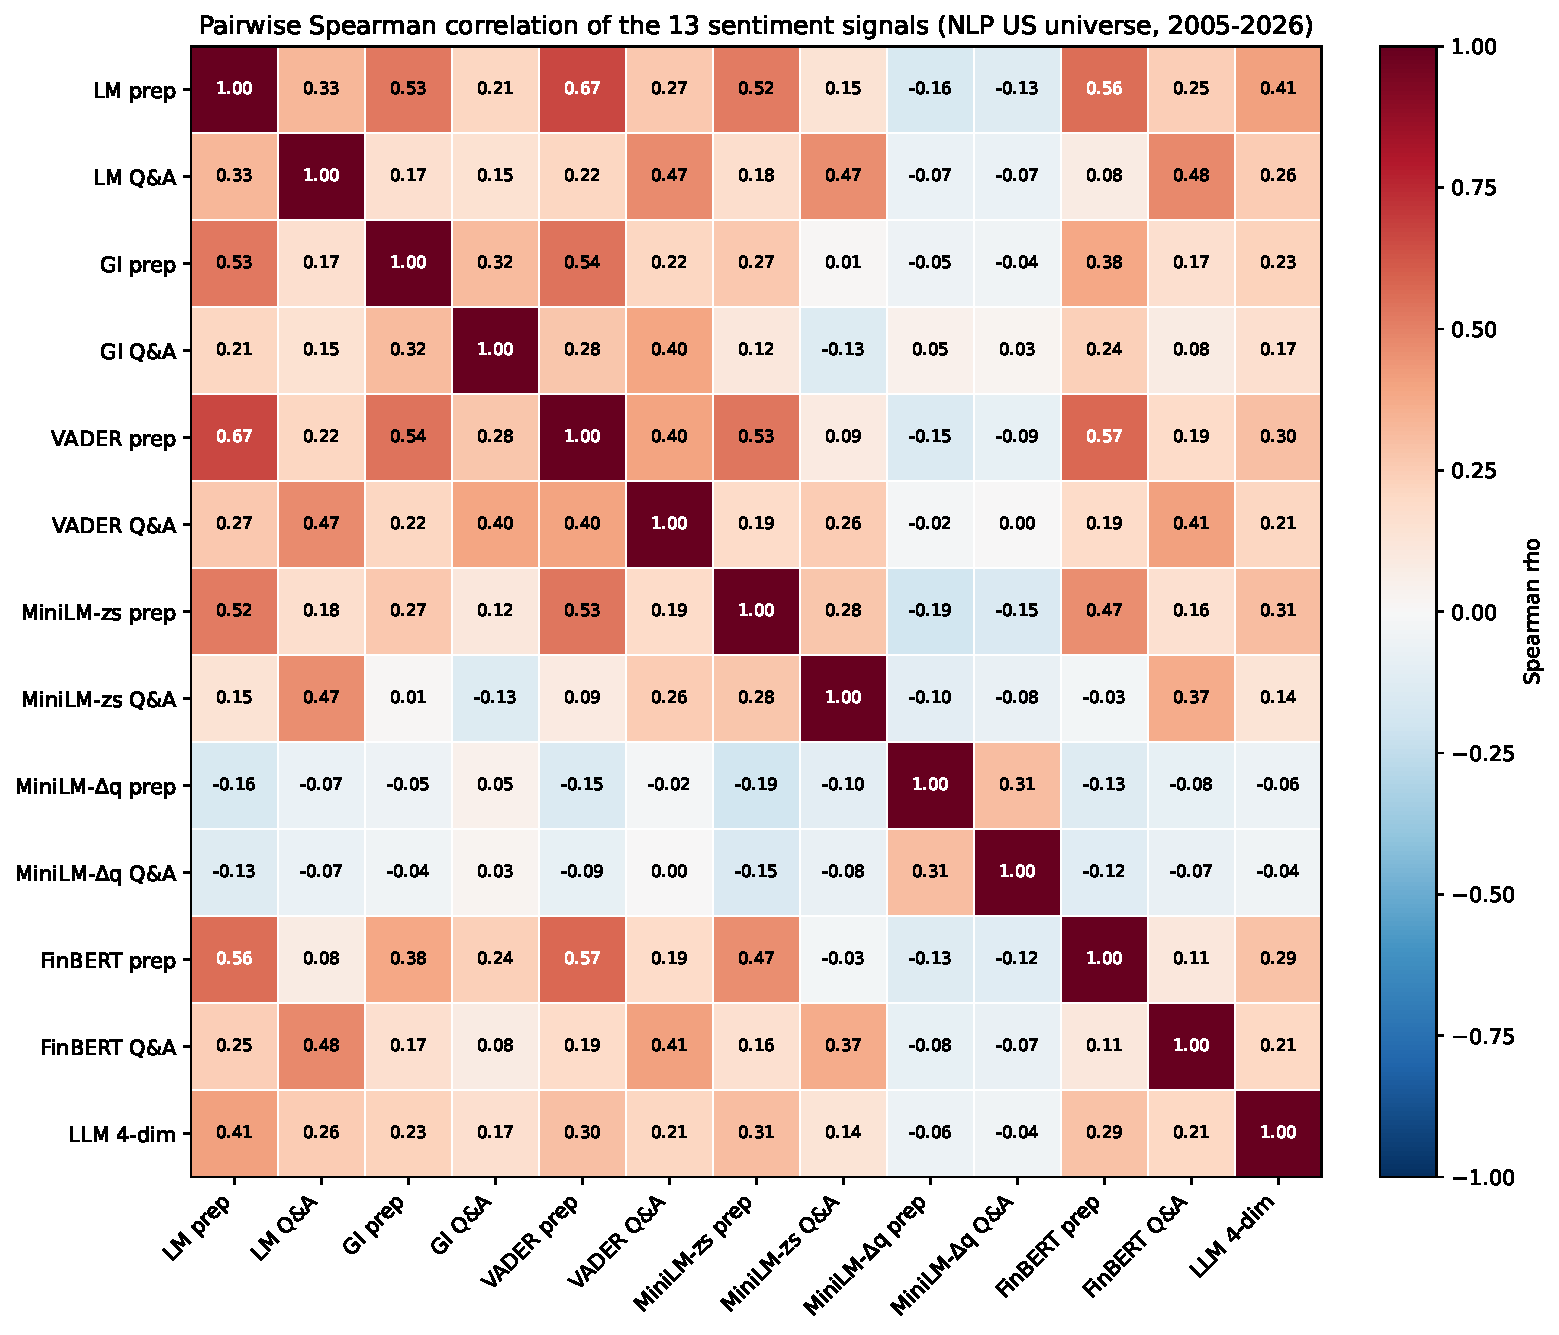
\includegraphics[width=0.7\linewidth]{files/figure_21_1_signal_d-c98aba29058901425df7938318f10c92.pdf}

It clarifies how much each method is a re-skinning of the others. The average off-diagonal correlation is 0.18, low enough that the methods are far from interchangeable on this sample. Four clusters stand out. The three tone-on-prepared-remarks dictionaries (LM prep, GI prep, VADER prep) cluster together at pairwise correlations of 0.4 to 0.5, with their Q\&A counterparts forming a parallel weaker cluster. FinBERT sits closer to the dictionaries than to the MiniLM family, consistent with the fact that it is a finance-domain fine-tune of a transformer trained to predict the same per-sentence sentiment categories (positive / neutral / negative) that the dictionaries operationalise. The two MiniLM $\Delta$quarter signals are near-orthogonal to every level-based signal, the expected signature of a textual-change construction that measures \textit{what moved} rather than \textit{what tone was struck}. The LLM 4-dim composite is largely orthogonal to every classical method, with pairwise correlations below 0.2 across the board, indicating that the four-axis decomposition (managerial confidence, specificity, surprise-negative, macro-vs-firm risk framing) is articulating dimensions that the single-scalar tone metrics simply do not see. The complementary correlations of each sentiment signal against the Fama-French / Carhart factor returns are reported in TABLE 21.2.

\paragraph{Spanning regression against Fama-French plus momentum}

A high information coefficient establishes that a signal carries cross-sectional information; it does not establish that the information is new. A sentiment score adds nothing to a portfolio already tilted on value, momentum, or quality if it merely re-expresses those exposures, so the question that decides whether a signal is worth trading is whether it earns a return the canonical equity-factor stack cannot explain. The standard tool for answering it is the \textit{spanning regression}, which regresses the signal's long-short portfolio return on the factor stack and reads the intercept as the part of that return the factors leave unexplained; we report it for every sentiment method in TABLE 21.2.

\textbf{TABLE 21.2: Spanning regressions of sentiment long-short portfolios on the Fama-French five-factor model augmented with Carhart momentum (US data, monthly, 2006-2026).} Following the convention of \cite{tetlock2007giving}, \cite{loughran2011liability}, and \cite{ke2019predicting}, we test whether each sentiment signal carries information \textit{net of} the canonical equity-factor stack by regressing its long-short portfolio return on the Fama-French five factors plus momentum. The construction is the standard \textit{monthly-rebalanced} one. At each month-end we forward-fill each stock's most recent earnings-call sentiment score (with a three-month stale-out, matching the natural quarterly call cadence), decile-sort the cross-section of stocks with a non-stale score, and form an equal-weighted long-short portfolio (top decile minus bottom decile). The realised one-month-forward return of each stock is taken from \texttt{mlfi\_us\_data} (column \texttt{R1M\_Usd}, the same monthly-return column used throughout the book). The cross-section requires at least 30 stocks to enter the sort. The resulting series is a non-overlapping monthly long-short return; spanning the 2006-2026 window yields 236 to 240 monthly observations per method. The factor returns (MKT-RF, SMB, HML, RMW, CMA, MOM) are pulled from Kenneth French's data library, the same source used in Chapter 3, with Newey-West HAC standard errors at five lags. The intercept (\texttt{Alpha}, annualised, in percent) tests whether the sentiment portfolio earns return unexplained by the six factors; the \texttt{R\textsuperscript{2}} measures how much of the sentiment-portfolio variance is \textit{explained} by FF6 (low R\textsuperscript{2} = orthogonal signal). Significance of the alpha intercept and of each factor loading, read from Newey-West t-statistics, is flagged with stars: * denotes p \textless  0.10, ** p \textless  0.05, *** p \textless  0.01.

\bigskip\noindent
\begin{tabular}{p{\dimexpr 0.091\linewidth-2\tabcolsep}p{\dimexpr 0.091\linewidth-2\tabcolsep}p{\dimexpr 0.091\linewidth-2\tabcolsep}p{\dimexpr 0.091\linewidth-2\tabcolsep}p{\dimexpr 0.091\linewidth-2\tabcolsep}p{\dimexpr 0.091\linewidth-2\tabcolsep}p{\dimexpr 0.091\linewidth-2\tabcolsep}p{\dimexpr 0.091\linewidth-2\tabcolsep}p{\dimexpr 0.091\linewidth-2\tabcolsep}p{\dimexpr 0.091\linewidth-2\tabcolsep}p{\dimexpr 0.091\linewidth-2\tabcolsep}}
\toprule
Method & n & Alpha (\%/yr) & t (NW) & R\textsuperscript{2} & $\beta$ MKT-RF & $\beta$ SMB & $\beta$ HML & $\beta$ RMW & $\beta$ CMA & $\beta$ MOM \\
\hline
Loughran-McDonald (prep, mgmt) & 240 & -1.9 & -0.61 & 0.012 & 0.08 & 0.00 & 0.00 & 0.07 & -0.11 & 0.02 \\
Loughran-McDonald (Q\&A, analysts) & 240 & -2.5 & -1.16 & 0.017 & 0.05 & -0.05 & -0.03 & 0.10 & 0.03 & 0.05 \\
Harvard GI (prep, mgmt) & 240 & -0.4 & -0.17 & 0.019 & 0.07 & -0.08 & -0.07 & -0.02 & 0.07 & -0.04 \\
Harvard GI (Q\&A, analysts) & 240 & +0.6 & +0.29 & 0.033 & -0.03 & 0.02 & -0.09 & -0.01 & -0.06 & 0.03 \\
VADER (prep, mgmt) & 240 & -3.5 & -1.47 & 0.029 & 0.08** & -0.00 & 0.06 & 0.02 & -0.13 & 0.00 \\
VADER (Q\&A, analysts) & 240 & -0.2 & -0.09 & 0.035 & -0.02 & -0.05 & -0.08 & 0.07 & -0.00 & 0.03 \\
MiniLM max-seed (prep, mgmt) & 240 & -4.4 & -1.64 & 0.111 & 0.17*** & -0.11 & 0.24** & -0.19* & -0.16 & 0.09** \\
MiniLM max-seed (Q\&A, analysts) & 240 & -4.3** & -2.14 & 0.037 & 0.06 & -0.04 & 0.16** & -0.07 & -0.08 & 0.08* \\
MiniLM $\Delta$quarter (prep, mgmt) & 237 & -1.6 & -0.76 & 0.046 & 0.03 & -0.18** & 0.15* & -0.02 & -0.22** & 0.02 \\
MiniLM $\Delta$quarter (Q\&A, analysts) & 236 & +0.7 & +0.41 & 0.007 & -0.02 & -0.06 & 0.01 & -0.06 & -0.04 & 0.00 \\
FinBERT (prep, mgmt) & 240 & -0.8 & -0.34 & 0.046 & 0.09** & -0.16* & 0.14 & -0.14 & -0.11 & -0.01 \\
FinBERT (Q\&A, analysts) & 240 & -0.6 & -0.39 & 0.028 & 0.06 & -0.11 & 0.08 & -0.12 & -0.04 & 0.05 \\
LLM 4-dim composite (Llama-3.1-8B) & 240 & +6.0* & +1.70 & 0.011 & 0.04 & -0.09 & 0.13 & -0.11 & -0.09 & 0.05 \\
\bottomrule
\end{tabular}

\bigskip

Three observations land cleanly on this table. First, the R\textsuperscript{2} values are uniformly small (between 0.01 and 0.11), which is the central methodological finding: every sentiment long-short portfolio in this table is largely \textit{orthogonal} to the six Fama-French / Carhart factors. The supplementary correlation matrix (computed alongside the table) confirms this: the largest pairwise correlation between any sentiment portfolio and any factor is 0.25 (MiniLM max-seed prep vs MKT-RF), with the bulk in the 0.00 to 0.15 range. Sentiment is not a hidden re-skinning of momentum or quality on this sample, and the one method that loads materially on the market and the value factors, MiniLM max-seed (prep), is also the method with the largest R\textsuperscript{2} (0.11) and therefore the most explained-away alpha. Second, no method clears the conventional 5\% alpha-significance threshold over this 20-year monthly panel. The closest are MiniLM max-seed (Q\&A) at -4.3\% per year (NW-t -2.14, just over the threshold but the wrong sign) and the LLM 4-dim composite at +6.0\% per year (NW-t +1.70, just under it). The LM, GI, VADER, MiniLM-$\Delta$quarter, and FinBERT alphas all sit between -3.5\% and +0.7\% with NW-t below 1.6 in absolute value. The upshot is that the strong univariate ICs reported in TABLE 21.1 do not translate into statistically significant portfolio alpha over a 240-month sample once the FF6 factor stack absorbs the systematic component. Third, the negative-sign alphas on MiniLM max-seed and VADER are consistent with the negative-IC pattern observed for the same methods in TABLE 21.1: the realised top-decile-minus-bottom-decile portfolio is sign-reversed and would be profitable as a contrarian bet, but neither the univariate IC nor the FF6 alpha is large enough to recommend it as a deployed strategy. The LLM 4-dim composite is the one entry whose alpha and direction both point the right way, but a marginally-significant +6.0\%/yr on a single 20-year US window is not yet evidence of a robust new factor; the look-ahead-bias caveats discussed in Chapter 23 (Llama-3.1-8B's training corpus overlaps the evaluation window) further temper that reading.

This orthogonality also settles a question the literature raises. \cite{habibah2021investor} find that \textit{aggregate} Baker-Wurgler sentiment drives the size and profitability premia; our firm-level signal does not, because a cross-sectional decile long-short differences out precisely the market-wide component a Baker-Wurgler index is built from. The two are both labelled ``sentiment'' but measure different objects, so a mirror regression of each premium on our signal returns loadings that are statistically zero across the board.

How was that table built? The construction is short enough to walk through in full, and worth doing because the single most common error in event-study NLP hides in one of its steps. The code below builds one method, Loughran-McDonald (prep); the full table is the same loop run over the other signal columns.

\begin{verbatim}
import pandas as pd
ff = pd.read_parquet('famafrench_us_factors.parquet')  # FF5 + MOM, monthly
panel = pd.read_parquet('sentiment_panel.parquet')     # per-call scores, keyed by secid = mlfi id
data_ml = pd.read_parquet('mlfi_us_data.parquet',
                          columns=['id', 'date', 'R1M_Usd'])
data_ml['month_end'] = data_ml['date'].dt.to_period('M').dt.to_timestamp('M')
ret = data_ml.rename(columns={'id': 'secid', 'R1M_Usd': 'R1M'})[['secid', 'month_end', 'R1M']]
\end{verbatim}

The forward-fill step takes each call's sentiment score and broadcasts it onto the \textbf{subsequent} month-ends only, with a three-month stale-out matching the natural quarterly call cadence; a newer call for the same firm supersedes the older one via \texttt{drop\_duplicates(keep='last')}. This is where the most common rookie error in event-study NLP sits, so we comment the look-ahead guard explicitly.

\begin{verbatim}
STALE = 3                                                         # months
calls = panel[['secid', 'date', 'lm_tone_prep_mgmt']].dropna()    # one method shown
calls['call_month'] = calls['date'].dt.to_period('M').dt.to_timestamp('M')
sig = pd.concat([calls.assign(month_end=calls['call_month'] + pd.offsets.MonthEnd(k))
                 for k in range(STALE)])                          # k=0,1,2: same / +1 / +2 mo
sig = (sig.sort_values(['secid', 'month_end', 'call_month'])
          .drop_duplicates(['secid', 'month_end'], keep='last')   # latest call wins
          .rename(columns={'lm_tone_prep_mgmt': 'signal'}))
\end{verbatim}

The portfolio step pairs the signal observed at month-end \textit{M} with the \texttt{R1M\_Usd} realised over the \textbf{following} month (\textit{M}, \textit{M}+1], never the same month. We require at least 30 stocks in the cross-section to enter the sort, dropping months that fall below that threshold rather than running five-stock deciles.

\begin{verbatim}
sig['next_month'] = sig['month_end'] + pd.offsets.MonthEnd(1)
df = sig.merge(ret.rename(columns={'month_end': 'next_month'}),
               on=['secid', 'next_month']).dropna()
ls = []
for m, sub in df.groupby('month_end'):
    if len(sub) < 30:                                             # min cross-section
        continue
    sub['bin'] = pd.qcut(sub['signal'], 10, labels=False, duplicates='drop')
    top = sub.loc[sub['bin'] == sub['bin'].max(), 'R1M'].mean()
    bot = sub.loc[sub['bin'] == 0, 'R1M'].mean()
    ls.append({'month_end': m, 'ls_ret': top - bot})
ls = pd.DataFrame(ls).set_index('month_end')['ls_ret']
\end{verbatim}

The spanning regression uses \texttt{statsmodels.OLS} with Newey-West HAC standard errors at five lags, the conventional choice for monthly portfolio returns since consecutive months' decile compositions overlap substantially.

\begin{verbatim}
import statsmodels.api as sm
joined = ff.join(ls, how='inner').dropna()
X = sm.add_constant(joined[['MKT_RF', 'SMB', 'HML', 'RMW', 'CMA', 'MOM']])
fit = sm.OLS(joined['ls_ret'], X).fit(cov_type='HAC', cov_kwds={'maxlags': 5})

def star(p):                                            # significance flags, as in TABLE 21.2
    return '***' if p < 0.01 else '**' if p < 0.05 else '*' if p < 0.10 else ''

facs = ['MKT_RF', 'SMB', 'HML', 'RMW', 'CMA', 'MOM']
alpha_ann = fit.params['const'] * 12 * 100              # annualised alpha, percent
print(f"n={int(fit.nobs)}  alpha_ann={alpha_ann:+.1f}%{star(fit.pvalues['const'])}  "
      f"t_NW={fit.tvalues['const']:+.2f}  R^2={fit.rsquared:.3f}")
print("  " + "  ".join(f"{f}={fit.params[f]:+.2f}{star(fit.pvalues[f])}" for f in facs))
\end{verbatim}

\begin{verbatim}
n=240  alpha_ann=-1.9%  t_NW=-0.61  R^2=0.012
  MKT_RF=+0.08  SMB=+0.00  HML=+0.00  RMW=+0.07  CMA=-0.11  MOM=+0.02
\end{verbatim}

The printed line reproduces the Loughran-McDonald (prep) row of TABLE 21.2 exactly, significance stars included; this method carries no coefficient significant at the 10\% level, so none are flagged, but pointing the same code at \texttt{embed\_zs\_prep\_mgmt} would reproduce the starred market, value, and momentum loadings of the MiniLM max-seed (prep) row.

\paragraph{Tree-based feature attribution}

The spanning regression of the previous subsection is linear and takes one signal at a time. A more demanding question is how a sentiment feature fares when it competes against the \textit{entire} book of firm characteristics inside a single nonlinear model. This is the machine-learning asset-pricing programme of \cite{gu2018empirical}, \cite{freyberger2020dissecting}, and \cite{nagel2021machine}: pool every predictor a quant would realistically use, let a gradient-boosted tree learn the nonlinear cross-sectional map to forward returns, and read off which inputs the fitted model actually relies on. We run that horse race with the earnings-call sentiment scores added to the book's own characteristic set.

We assemble a quarterly \textit{bundle}: the 122 numerical characteristics of the book's US panel, of the kind catalogued by \cite{chen2021open}, joined to the 32 sentiment scores of the companion dataset. The 32 scores are the nine per-bucket sentiment methods of TABLE 21.1 taken over the three speech buckets, together with five structural counts; the companion \texttt{sentiment\_panel.parquet} also carries auxiliary columns (forward returns, regime tags, model rationales) that we exclude from the feature set; the file is already keyed to the book's numerical \texttt{id}. The join is the look-ahead-safe forward-fill of the earlier subsections; each call's scores attach only to quarter-ends on or after the call date, within a two-quarter stale-out.

\begin{verbatim}
import pandas as pd
dml = pd.read_parquet('mlfi_us_data.parquet')                       # 122 numerical characteristics
labels = ['R1M_Usd', 'R3M_Usd', 'R6M_Usd', 'R12M_Usd']
classic = [c for c in dml.columns if c not in ['id', 'date'] + labels]
q = dml[dml['date'].dt.month.isin([3, 6, 9, 12])].copy()           # quarter-end rows only
q['date'] = q['date'].astype('datetime64[ns]')

panel = pd.read_parquet('sentiment_panel.parquet')                 # per-call earnings scores, with id
buckets = ['prep_mgmt', 'qa_mgmt', 'qa_analyst']                    # 32 canonical sentiment scores:
methods = ['finbert', 'gi_tone', 'lm_tone', 'lm_neg_pct', 'lm_pos_pct',   # nine methods x three
           'lm_unc_pct', 'vader', 'embed_zs', 'embed_dist']              # speech buckets (27) plus
sent = [f'{m}_{b}' for m in methods for b in buckets] + [           # five structural counts (5) = 32
    'fog', 'text_distance', 'n_words', 'n_money', 'n_percent']
panel['date'] = panel['date'].astype('datetime64[ns]')
panel = panel.dropna(subset=['id']).astype({'id': 'int'})[['id', 'date'] + sent]
\end{verbatim}

The forward-fill join then attaches each firm's most recent call to every quarter-end, and the classical and sentiment columns are concatenated into the 154-feature design matrix.

\begin{verbatim}
# latest call on-or-before each quarter-end, within ~2 quarters (look-ahead-safe)
bundle = pd.merge_asof(q.sort_values('date'), panel.sort_values('date'),
                       on='date', by='id', direction='backward',
                       tolerance=pd.Timedelta('185D'))
bundle = bundle.dropna(subset=['R3M_Usd', 'lm_tone_prep_mgmt'])     # need label + sentiment coverage
bundle['year'] = bundle['date'].dt.year
feats = classic + sent                                             # 122 + 32 = 154 features
\end{verbatim}

The target is the cross-sectional percentile rank of the next-quarter return \texttt{R3M\_Usd}. Ranking within each quarter removes the market-wide component, which no stock-level feature can forecast, and points the model at the cross-sectional stock-picking task.

\begin{verbatim}
bundle['y'] = bundle.groupby('date')['R3M_Usd'].rank(pct=True)      # per-quarter percentile target
\end{verbatim}

The validation protocol is a strict expanding window. The first ten years form the initial training set; the model is retrained every calendar year and used to predict only the \textit{following} year out of sample, so no fold sees its own future. Feature importance is computed with SHAP on each year's out-of-sample rows, using the model trained on strictly prior data, and pooled across folds. The booster is deliberately shrunk to survive the low signal-to-noise of quarterly returns: 400 shallow trees at a slow learning rate, with row and column subsampling.

\begin{verbatim}
import xgboost as xgb, shap
params = dict(n_estimators=400, max_depth=4, learning_rate=0.01,   # slow, shallow, regularized
              subsample=0.8, colsample_bytree=0.6, min_child_weight=5,
              reg_lambda=1.0, objective='reg:squarederror', random_state=42)
years = sorted(bundle['year'].unique())
shap_pool, imp_year = [], {}
for y in [t for t in years if t >= years[0] + 10]:                 # >= 10y train, retrain each year
    tr = bundle[bundle.year < y]; te = bundle[bundle.year == y]    # expanding train, next-year OOS
    fit = xgb.XGBRegressor(**params).fit(tr[feats], tr['y'])
    shap_pool.append(shap.TreeExplainer(fit).shap_values(te[feats]))    # SHAP on OOS rows only
    imp_year[y] = pd.Series(fit.feature_importances_, index=feats)      # gain importance this fold
\end{verbatim}

Two diagnostics frame the result before the ranking. Out of sample the model earns a mean cross-sectional information coefficient of 0.010 across the eleven annual folds, weakly positive and positive in seven of the eleven years. In squared-error terms it barely separates from the naive benchmark that predicts the median rank: the pooled out-of-sample MSE bottoms out around 35 trees and drifts back above the benchmark thereafter, the shallow-signal, quick-to-overfit regime typical of return prediction, in which measured predictability is, as \cite{avramov2023machine} document, concentrated in hard-to-arbitrage stocks and fragile to economic restrictions and trading costs. The quarterly cross-section is hard, and the exercise is about \textit{relative} importance, not a tradeable forecast. With that caveat, we report the pooled out-of-sample SHAP ranking of all 154 features in TABLE 21.3.

\textbf{TABLE 21.3: Pooled out-of-sample SHAP feature ranking, all 154 features, 2015-2025.} Mean absolute SHAP value of each feature, computed on the out-of-sample rows of each annual expanding-window fold and pooled across folds. The \texttt{family} column is the ten-way factor-taxonomy assignment used for the family breakdown below. Only the top 15 of 154 features are shown.

\bigskip\noindent
\begin{tabular}{p{\dimexpr 0.250\linewidth-2\tabcolsep}p{\dimexpr 0.250\linewidth-2\tabcolsep}p{\dimexpr 0.250\linewidth-2\tabcolsep}p{\dimexpr 0.250\linewidth-2\tabcolsep}}
\toprule
Rank & Feature & Family & Mean abs SHAP \\
\hline
1 & Book\_Value\_PS & Value & 0.0061 \\
2 & rsi\_14 & Momentum & 0.0056 \\
3 & EPS & Value & 0.0044 \\
4 & macd & Momentum & 0.0039 \\
5 & vol\_22 & Volatility & 0.0023 \\
6 & size\_log & Size & 0.0019 \\
7 & Earnings\_Volatility\_Proxy & Quality & 0.0018 \\
8 & llm\_specificity & Sentiment & 0.0017 \\
9 & GP\_to\_Assets\_Novy\_Marx & Profitability & 0.0016 \\
10 & FCF\_yld & Value & 0.0015 \\
11 & beta\_252d & Volatility & 0.0015 \\
12 & FCF\_to\_TBV & Profitability & 0.0015 \\
13 & EPS\_Growth\_1Y & Growth & 0.0014 \\
14 & rel\_str\_252d & Momentum & 0.0014 \\
15 & embed\_zs\_qa\_analyst & Sentiment & 0.0014 \\
\bottomrule
\end{tabular}

\bigskip

The ranking is clear and sobering. The top of the table is owned by classical value and technical characteristics (book value, RSI, earnings, MACD, short-horizon volatility, size), the families that the characteristics-only work of \cite{freyberger2020dissecting} and \cite{han2024cross} repeatedly ranks on top, and that the explainable-AI study of \cite{goswami2025significance}, run over 166 predictors, leads with as well. The strongest sentiment feature, the LLM-derived \textit{specificity} score, ranks eighth, ahead of most fundamentals but behind the leaders; the zero-shot embedding score on analyst Q\&A follows at fifteenth. Four sentiment features reach the top twenty and nine the top fifty, a genuine presence rather than a rounding error, yet the four-axis LLM composite that would head a small, hand-picked baseline falls to twenty-sixth once it must compete against the full characteristic set. We plot the SHAP beeswarm for the fifteen leading features, pooled across the eleven annual out-of-sample folds (2015-2025), in FIGURE 21.2.

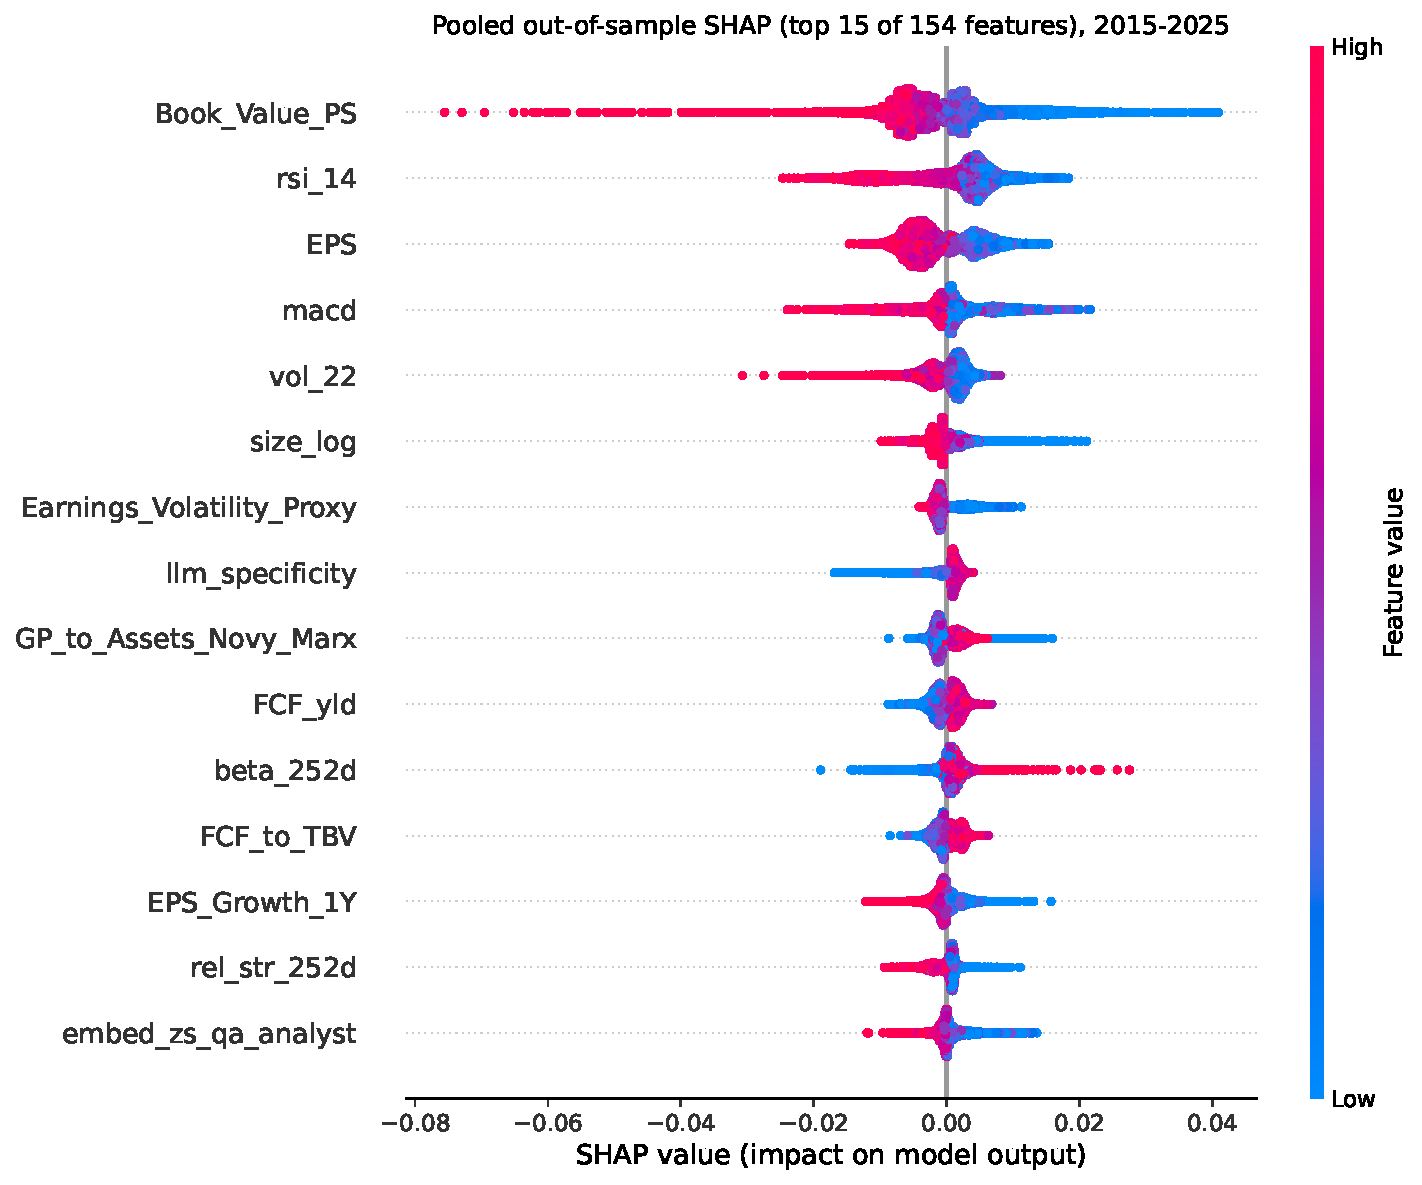
\includegraphics[width=0.7\linewidth]{files/figure_21_2_shap_bee-c4682eafcae615f3a58d916cd47a7d81.pdf}

In FIGURE 21.2 each dot is one out-of-sample firm-quarter, its horizontal position the feature's SHAP contribution to the predicted return rank, and its colour the feature value. The leaders show clean monotone colour gradients; the sentiment features carry diffuse, near-symmetric contributions, the signature of a weak but non-zero signal.

The relative standing of the leading features is broadly stable through time, as the gain-importance paths of FIGURE 21.3 show: the same value, momentum, and volatility characteristics dominate every retrain, their ordering drifting modestly from one year to the next rather than settling into a fixed rank, and the single sentiment feature among the SHAP leaders, LLM specificity, holds a mid-pack line throughout.

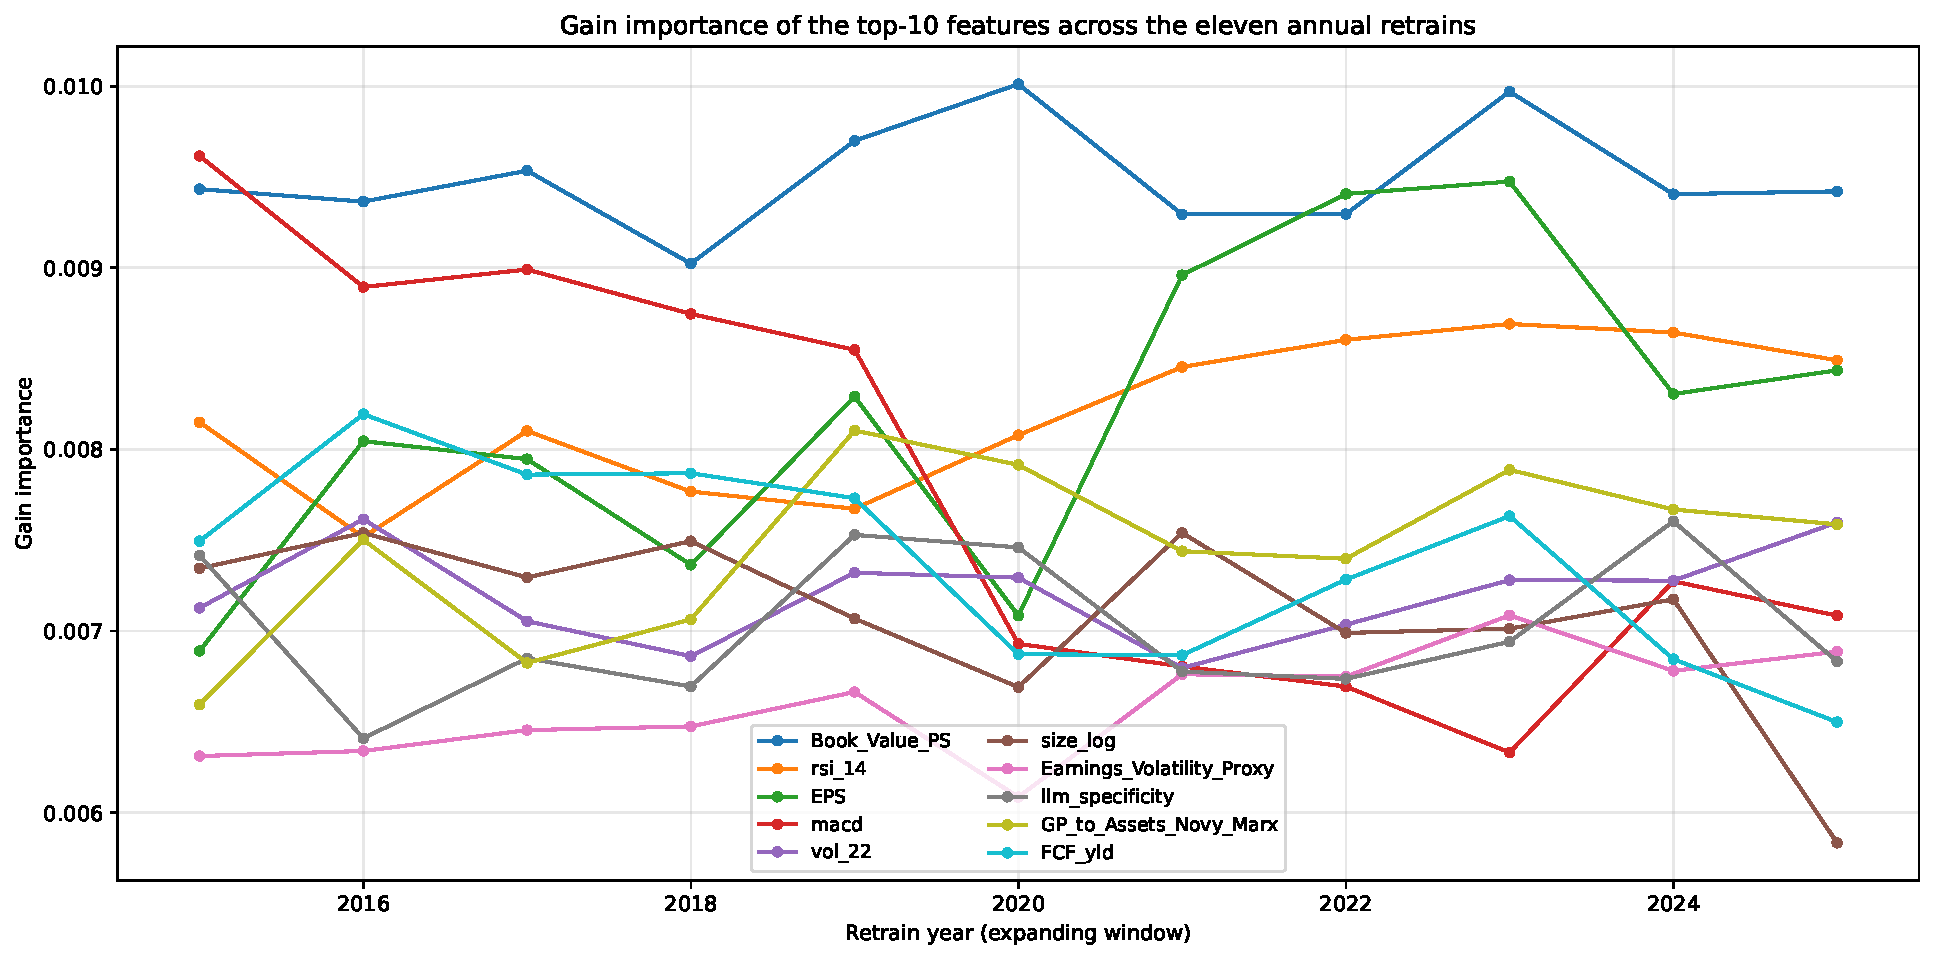
\includegraphics[width=0.7\linewidth]{files/figure_21_3_importan-014d5c1d1f979ba6b51b9e117ad82a23.pdf}

To summarise across all 154 features we group them into ten factor families (value, profitability, quality, growth, investment, momentum, size, volatility, liquidity, and sentiment) and sum the normalised importance within each family for every retrain year, plotting the shares in FIGURE 21.4.

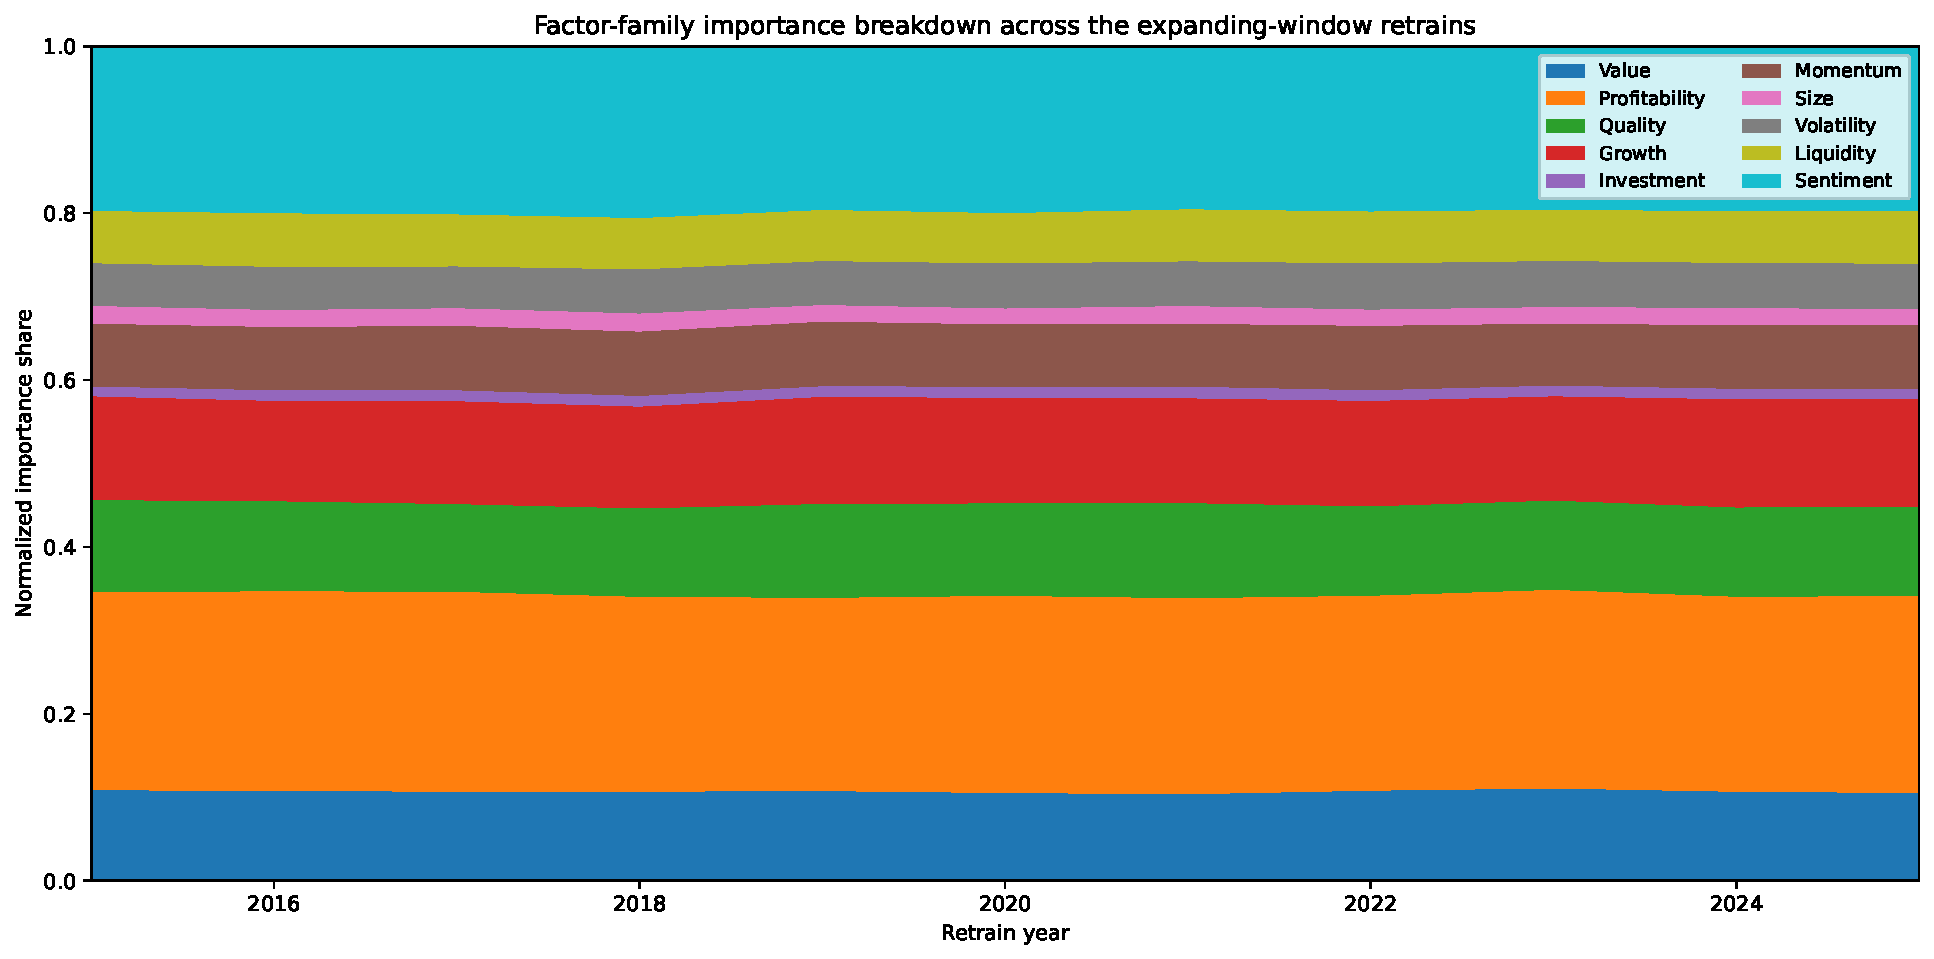
\includegraphics[width=0.7\linewidth]{files/figure_21_4_family_b-fc2726191923f112c5e85240626998b5.pdf}

The family breakdown of FIGURE 21.4 is the headline of this subsection, and it cuts both ways. As a \textit{bloc}, sentiment is the second-largest family the model draws on, taking roughly a fifth of total importance behind only profitability, and its share is steady from 2015 to 2025. But that twenty-percent bloc is almost exactly proportional to headcount, because sentiment supplies 32 of the 154 features. Dividing each family's importance by its number of features, the per-feature contribution is nearly uniform across all ten families, close to ten percent each, with sentiment fractionally at the bottom. The gradient booster, in other words, spreads its reliance evenly: no family, sentiment included, punches above its weight per input. That breadth is literal rather than nominal: the booster picks every one of the thirty-two sentiment scores in at least three of the eleven folds, discarding none of them outright, even though the weakest (the Loughran-McDonald positive-word share on the management Q\&A, which lands 144th of 154) carries a mean absolute SHAP value some fifty times smaller than the leading characteristic. Sentiment earns its collective place through breadth, not through any single dominant score.

The family breakdown treats each feature's importance as a single scalar, and it says nothing about where in the model a score is consulted. To close the subsection we look inside the ensemble itself and extract one of its 400 trees. Below, we plot tree 100, a single full-sample fit that shares the hyperparameters of the expanding-window model of Section 21.7.4, and shade the splits that use a sentiment feature. The result appears in FIGURE 21.5.

\begin{verbatim}
# One tree from the ensemble: a single full-sample fit with the Section 21.7.4
# hyperparameters, used only to look inside the split structure.
import xgboost as xgb
bundle['y'] = bundle.groupby('date')['R3M_Usd'].rank(pct=True)          # per-quarter percentile target
fit_full = xgb.XGBRegressor(**params).fit(bundle[feats], bundle['y'])   # params from Section 21.7.4
tree = fit_full.get_booster().trees_to_dataframe().query('Tree == 100').set_index('ID')
print('root split feature:', tree.loc['100-0', 'Feature'])             # the leading momentum characteristic
\end{verbatim}

\begin{verbatim}
root split feature: rsi_14
\end{verbatim}

With the node table in hand, we assign coordinates, spreading the leaves evenly and centring each interior node above its two children.

\begin{verbatim}
# Lay the tree out: leaves left to right, each interior node centered above its children.
pos, leaves = {}, []
def place(nid, depth):
    node = tree.loc[nid]
    if node.Feature == 'Leaf':
        leaves.append(nid); pos[nid] = (len(leaves) - 1.0, -depth); return pos[nid][0]
    x = (place(node.Yes, depth + 1) + place(node.No, depth + 1)) / 2    # midpoint of the two children
    pos[nid] = (x, -depth); return x
place('100-0', 0)
\end{verbatim}

We then draw the tree, shading the interior nodes that split on a sentiment feature so they stand out from the classical ones.

\begin{verbatim}
# Draw the tree; sentiment splits are shaded to separate them from the classical splits.
import matplotlib.pyplot as plt
from matplotlib.patches import FancyBboxPatch
fmt = lambda s: '~0' if abs(s) < 1e-6 else f'{s:.3g}'                   # tidy near-zero thresholds
fig, ax = plt.subplots(figsize=(15, 7))
for nid, node in tree.iterrows():
    x, y = pos[nid]
    if node.Feature == 'Leaf':
        ax.text(x, y, f'{node.Gain:+.3f}', ha='center', va='center', fontsize=7, color='#445566'); continue
    is_sent = node.Feature in set(sent)                                # sentiment features get shaded, bold boxes
    for child in (node.Yes, node.No):
        ax.plot([x, pos[child][0]], [y - 0.06, pos[child][1] + 0.06], color='#99aaaa', lw=0.8, zorder=1)
    ax.add_patch(FancyBboxPatch((x - 0.9, y - 0.06), 1.8, 0.12, boxstyle='round,pad=0.02', zorder=2,
                 fc='#f4a259' if is_sent else '#dfe7ef', ec='#c26b18' if is_sent else '#9fb0c0',
                 lw=1.4 if is_sent else 0.8))
    ax.text(x, y, f'{node.Feature}\n< {fmt(node.Split)}', ha='center', va='center', zorder=3,
            fontsize=8, fontweight='bold' if is_sent else 'normal')
ax.set_xlim(-1.5, len(leaves)); ax.set_ylim(-4.6, 0.6); ax.axis('off')
plt.tight_layout(); plt.savefig('images/figure_21_5_ensemble_tree.png', dpi=150, bbox_inches='tight')
\end{verbatim}

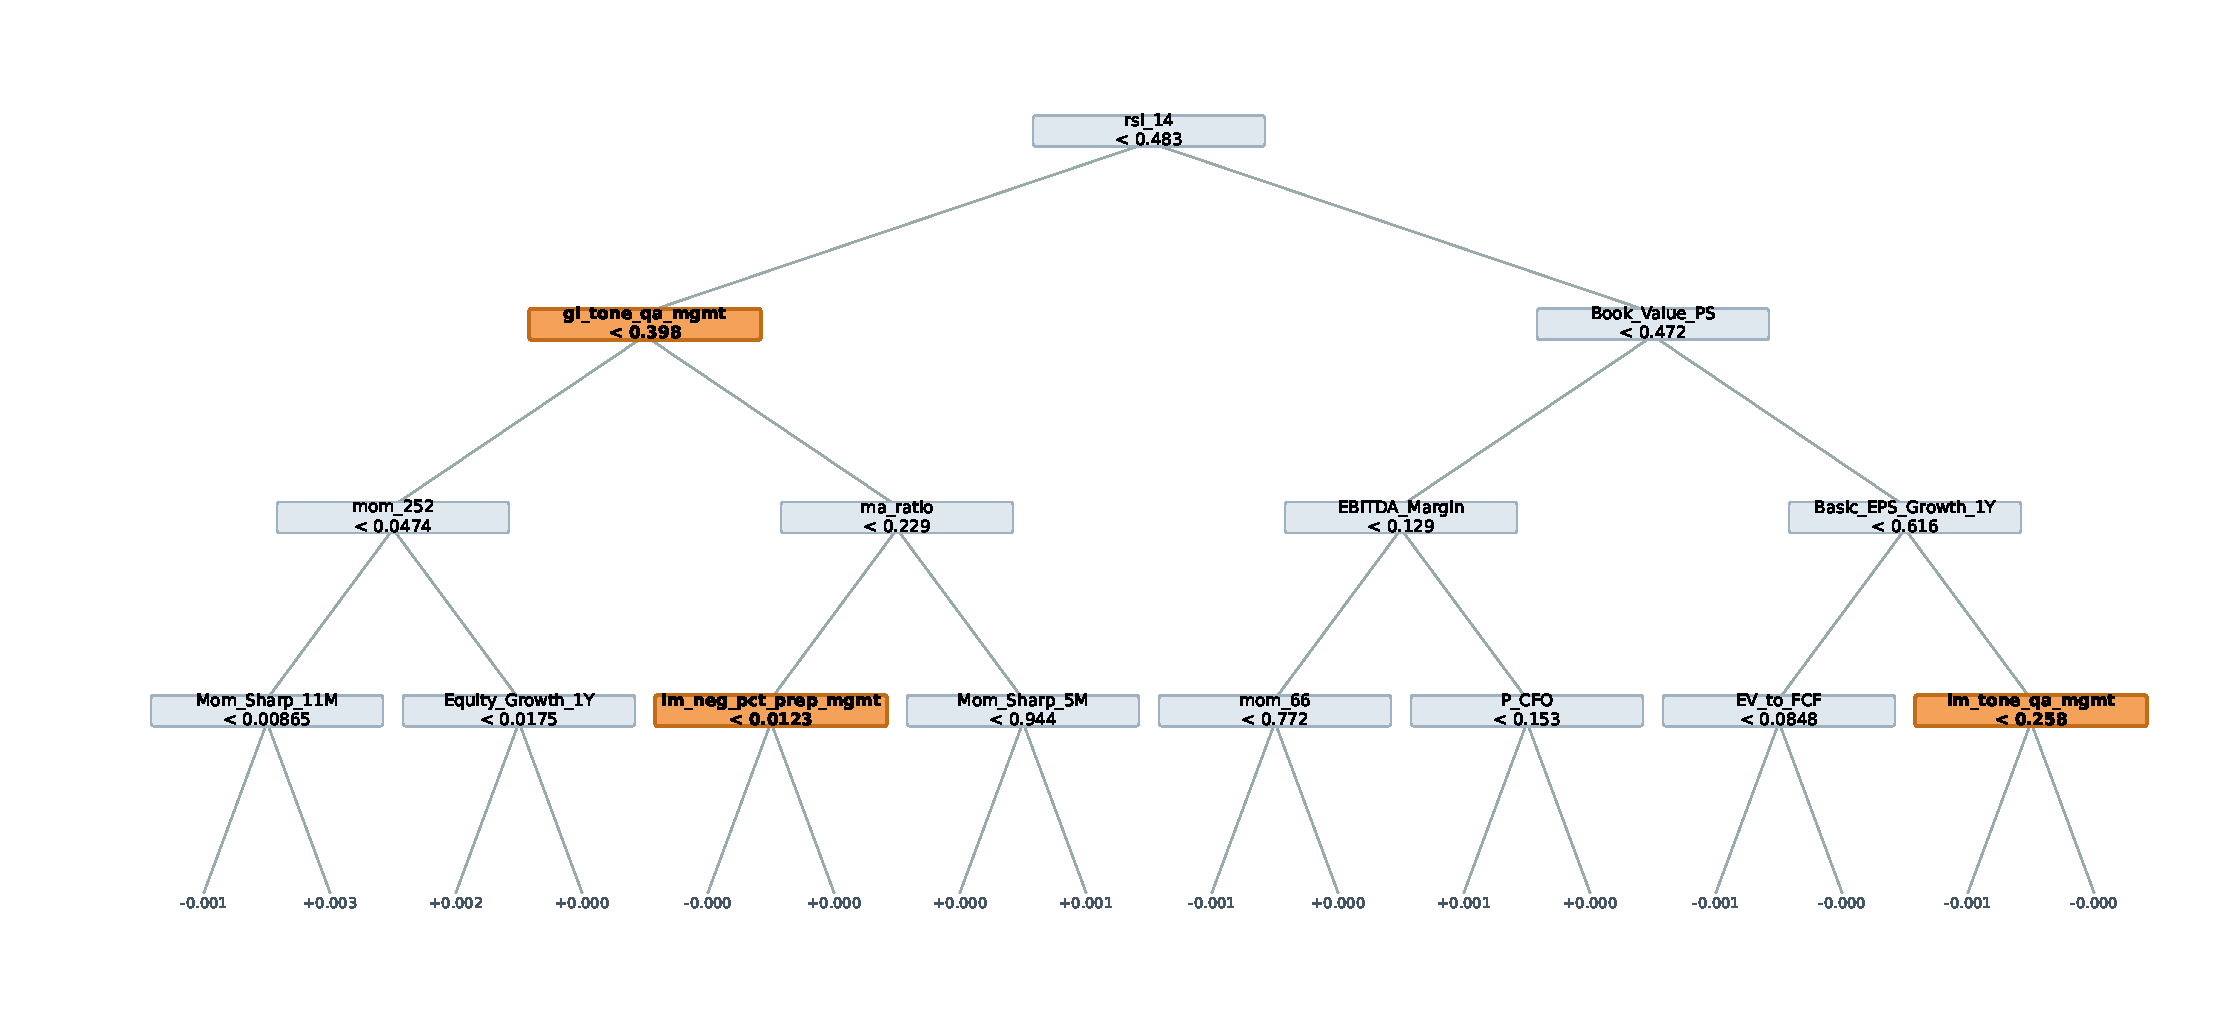
\includegraphics[width=0.7\linewidth]{files/figure_21_5_ensemble-64a8403ad570f013a0e3d710ee52651f.pdf}

The tree of FIGURE 21.5 is revealing. Its root split, the feature the booster consults first for every firm-quarter, is the fourteen-day RSI, a classical momentum characteristic, and the first two levels are dominated by the value, momentum, and volatility characteristics (book value per share, medium-horizon momentum, EBITDA margin) that head the ranking. Sentiment is not shut out of that early geometry, however: a GI-tone score on the management Q\&A splits one level below the root, the LLM-derived specificity score enters at the second level, and a FinBERT prepared-remarks score at the third, three sentiment nodes interleaved with the classical splits rather than relegated to the leaves as residual tie-breakers. We should not over-read a single tree, since it is one of 400 in a learning-rate-0.01 ensemble and its own leaf adjustments are tiny, of the order 0.001 to 0.003 in percentile-rank units, so the aggregate signal remains the weak one documented above. What the tree makes visible is where the sentiment scores enter the model, not that any one of them forecasts returns on its own.

This nonlinear attribution and the linear spanning regression of Section 21.7.3 agree from two directions. The spanning regression found the sentiment portfolios orthogonal to the factor stack, with no reliably significant alpha; the tree finds the individual sentiment features informative but mid-tier, contributing in proportion to their number rather than commanding the model. Neither result places a single text signal above the traditional factors; both cast text-derived features as a genuine, incremental, and unspectacular ingredient. The finding sits between two poles of the literature. At the characteristics-only pole, the linear shrinkage of \cite{kozak2019shrinking} and the nonparametric selection of \cite{freyberger2020dissecting} both recover most cross-sectional predictability from price-trend, liquidity, and volatility characteristics with no text at all. At the text-in-isolation pole, purpose-built text turns first-order when it is the sole input or faces a weak baseline, whether the SESTM learner of \cite{ke2019predicting}, the machine-learning photo-and-text pessimism index of \cite{obaid2022picture}, the priced constraint measure of \cite{buehlmaier2018financial}, or the LLM investment scores of \cite{jha2024chatgpt}. What almost no study reports is the within-model head-to-head we run here, text and the full characteristic panel competing inside one estimator; the textual-factor programme of \cite{cong2019textual} is the closest large-scale precedent, and the manager-sentiment evidence of \cite{jiang2019manager} mirrors our split, with sentiment strong in the aggregate but weaker and conditional in the cross-section.

\paragraph{Sentiment for conditioning factors}

The tree attribution above pools across market conditions. The natural next question is whether sentiment conditions \textit{when} a factor overlay pays off: do the overlays earn their contribution evenly, or only in particular sentiment regimes? The question has a long lineage. A large literature establishes that factor and anomaly premia are not regime-invariant but load on the aggregate sentiment state. \cite{baker2006investor} show that the cross-sectional predictability of hard-to-arbitrage stocks (small, young, volatile, unprofitable, distressed) is itself sentiment-conditional, and \cite{stambaugh2012short} sharpen the point for anomalies: long-short returns are large and significant only following high-sentiment months, and the effect is concentrated in the short leg, where overpricing is hardest to arbitrage away. The same conditioning recurs across the factor zoo, in momentum \citep{antoniou2013cognitive}, in the risk-return tradeoff \citep{yuyuan2011investor}, and in the slope of the security market line \citep{antoniou2016investor}. We therefore characterise the prevailing sentiment regime, shown in FIGURE 21.6, and stratify the Sharpe ratio of each portfolio configuration by it in TABLE 21.4.

Below, we build the regime state variable from the earnings-call panel, the per-quarter cross-sectional mean of the FinBERT sentiment score, and sort the quarters into terciles.

\begin{verbatim}
# The regime state variable: per-quarter cross-sectional mean of the FinBERT
# earnings-call sentiment, sorted into low, medium, and high terciles.
import pandas as pd
sent = pd.read_parquet('sentiment_panel.parquet')
fb = ['finbert_prep_mgmt', 'finbert_qa_mgmt', 'finbert_qa_analyst']     # three call segments
sent = sent[sent['secid'].notna()].copy()
sent['s_mean'] = sent[fb].mean(axis=1, skipna=True)                     # per-call sentiment
sent['quarter'] = sent['date'].dt.to_period('Q').dt.to_timestamp('Q')
s_mkt = sent[sent['quarter'] <= '2026-03-31'].groupby('quarter')['s_mean'].mean()
regime = pd.qcut(s_mkt, 3, labels=['Low', 'Med', 'High'])              # sentiment-regime terciles
\end{verbatim}

We then plot the composite, shading each quarter with a full-height pane in its regime colour.

\begin{verbatim}
# Plot the composite; a full-height background pane colors each quarter by regime.
import matplotlib.pyplot as plt
from matplotlib.patches import Patch
colors = {'Low': '#4c72b0', 'Med': '#b0b0b0', 'High': '#c44e52'}       # cool / grey / warm
q = s_mkt.index
edges = list(q[:-1] + (q[1:] - q[:-1]) / 2)                            # midpoints between quarters
edges = [q[0] - (edges[0] - q[0])] + edges + [q[-1] + (q[-1] - edges[-1])]
fig, ax = plt.subplots(figsize=(11, 4.5))
for i, r in enumerate(regime):
    ax.axvspan(edges[i], edges[i + 1], color=colors[r], alpha=0.16, lw=0, zorder=0)
ax.plot(q, s_mkt.values, color='#333', lw=1.2, marker='o', ms=3.2, zorder=2)
ax.set_xlabel('quarter'); ax.set_ylabel('aggregate sentiment $S_{mkt}$')
ax.legend(handles=[Patch(fc=colors[r], alpha=0.5, label=f'{r} sentiment')
                   for r in ['Low', 'Med', 'High']], ncol=3, frameon=False)
plt.savefig('images/figure_21_6_sentiment_regime.png', dpi=150, bbox_inches='tight')
\end{verbatim}

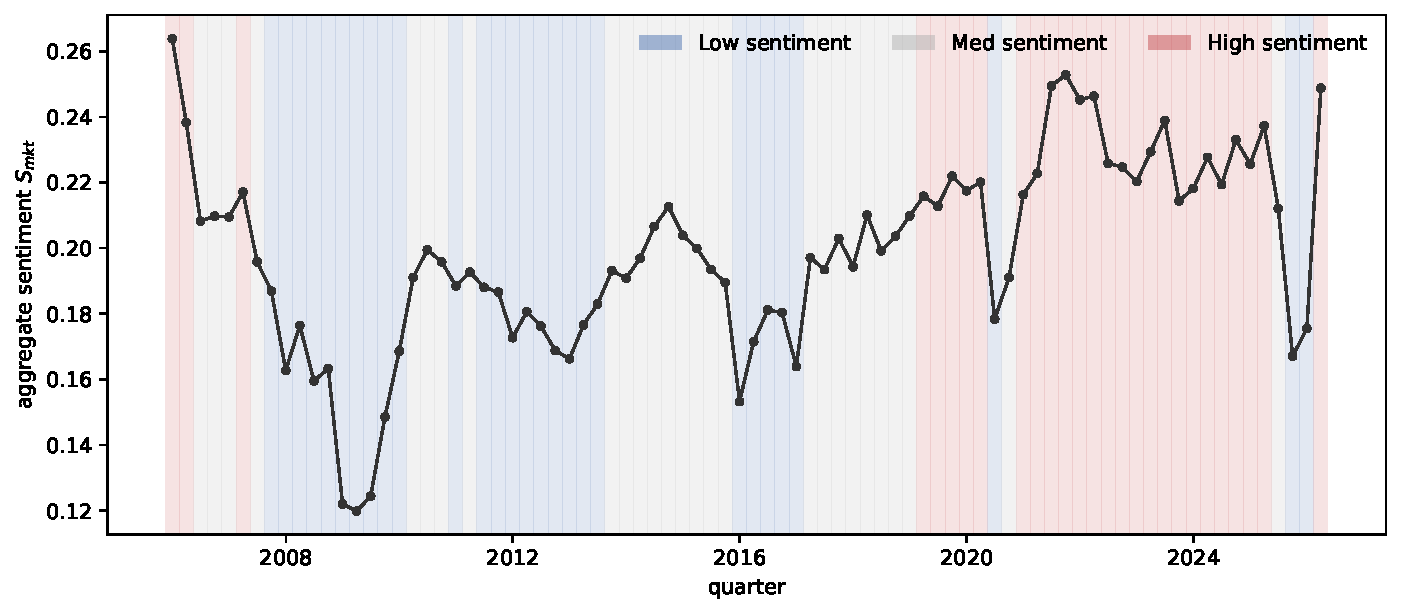
\includegraphics[width=0.7\linewidth]{files/figure_21_6_sentimen-af7a398b47e374892a5e17c6d7756307.pdf}

The regime shown in FIGURE 21.6 is economically legible rather than an artefact of the sorting. The composite sits in its low tercile through the crisis quarters, reaching its sample minimum in the 2008-2009 financial crisis and dipping again in 2016 and during the 2020 pandemic shock, and in its high tercile through the calm expansions of 2006-2007 and 2021-2025. That the tercile of an aggregate earnings-call tone lines up with the familiar risk-on and risk-off phases of the cycle is what lets it serve as a conditioning state rather than noise, and it is this state that TABLE 21.4 stratifies against.

\textbf{TABLE 21.4: Regime-stratified Sharpe ratios, following the sentiment-regime construction of \cite{grobys2021factor}.} Sharpe of each portfolio configuration is reported separately within terciles of an aggregate sentiment composite (low / medium / high) over the same NLP US universe.

\bigskip\noindent
\begin{tabular}{p{\dimexpr 0.250\linewidth-2\tabcolsep}p{\dimexpr 0.250\linewidth-2\tabcolsep}p{\dimexpr 0.250\linewidth-2\tabcolsep}p{\dimexpr 0.250\linewidth-2\tabcolsep}}
\toprule
Configuration & Low & Medium & High \\
\hline
Traditional 6-factor (baseline) & -0.45 & +0.19 & -0.37 \\
+ Loughran-McDonald overlay & -0.40 & +0.05 & -0.97 \\
+ FinBERT prepared overlay & -0.47 & +0.09 & -0.60 \\
+ FinBERT Q\&A overlay & -0.19 & -0.08 & -0.62 \\
+ MiniLM max-seed overlay [baseline] & -0.58 & -0.28 & -0.53 \\
+ MiniLM $\Delta$quarter overlay & -0.38 & +0.06 & -0.55 \\
+ LLM 4-dim overlay (Llama-3.1-8B) & -0.26 & -0.08 & +0.76 \\
+ All-sentiment composite & -0.39 & -0.12 & -0.88 \\
\bottomrule
\end{tabular}

\bigskip

The regime is operationalised as simply as possible: we sort months into terciles of an aggregate sentiment composite and compute the Sharpe of each configuration within each tercile, following the sentiment-conditioning approach that \cite{grobys2021factor} apply to factor momentum. Cleaner state variables are available, among them the partial-least-squares aligned sentiment index of \cite{huang2015investor} and the Markov regime-switching formulation of \cite{chung2012when}, but the tercile split keeps the conditioning transparent and avoids fitting a regime model on the same short sample.

The result cuts against the grain of that literature, and instructively so. The classical overlays, the Loughran-McDonald, FinBERT Q\&A, MiniLM max-seed, and all-sentiment-composite configurations, all collapse in the high-sentiment regime, with Sharpes ranging from -0.53 to -0.97. This is the reverse of what the canon would predict for a genuine mispricing factor: \cite{stambaugh2012short} find anomaly premia are largest, not smallest, following high sentiment, and \cite{grobys2021factor} report that factor momentum is more pronounced when sentiment is high. The most economical reading of our table is that these sentiment overlays are largely contrarian bets whose edge is already priced by the time aggregate sentiment is elevated, so a long-short sort on the signal has little left to harvest. The MiniLM $\Delta$quarter overlay (Lazy Prices on embeddings) is the only embedding configuration to recover a small positive Sharpe (+0.06) in the medium regime, but it too collapses in the high regime (-0.55): the textual-change signal carries genuine information about firm-level dispersion yet does not escape the regime-conditioning that affects every level-based or change-based classical method.

The single exception is the LLM 4-dim overlay, the only configuration with a positive Sharpe in the high-sentiment regime (+0.76 against a baseline of -0.37 and a worst-overlay of -0.97). It is, in other words, the only overlay that behaves the way the classical literature says a genuine mispricing factor should, earning its premium precisely when sentiment-driven overpricing is most acute. We read this as the LLM's four-axis decomposition, managerial confidence net of the macro-vs-firm risk-framing dimension, capturing a textual signal that the classical methods compress into a single sentiment scalar and therefore mistime in exactly the high-sentiment states where it matters most.

Two cautions temper the reading before it hardens into a claim. First, the sample window is finite, and conditional asset-pricing tests are notoriously easy to fool: \cite{novymarx2014predicting} shows that patently spurious conditioning variables, from the weather to sunspots, appear to ``predict'' anomaly performance about as well as economically motivated ones, so a single regime-stratified table is suggestive rather than decisive. Second, the pattern may not travel; \cite{salurekinci2023anomalies} find the sentiment-anomaly link is not universal internationally and is heavily mediated by the size factor. We therefore read TABLE 21.4 as an indicative empirical regularity, consistent with the modern text-sentiment strand that builds the regime bottom-up from language rather than from a slow survey index \citep{garcia2013sentiment, calomiris2019news}, and sufficiently striking to be worth flagging as a research direction rather than as evidence of a robust new factor.

\subsubsection{Coding exercises}

\begin{enumerate}
\item Using the \texttt{gensim} library or a similar implementation, train a Word2Vec
model on a corpus of financial text (e.g., a set of 10-K filings from
SEC EDGAR, or a collection of news headlines from a public dataset).
Examine the resulting embedding space by computing the nearest neighbours
of a handful of financial terms (\texttt{growth}, \texttt{risk}, \texttt{dividend},
\texttt{acquisition}). Do the neighbours match your domain intuition?
\item Download a pre-trained sentence-transformer model (e.g., \texttt{all-MiniLM-L6-v2}
from the \texttt{sentence-transformers} library). Encode the business-description
sections of 50 firm 10-K filings, compute the pairwise cosine-similarity
matrix, and visualise the resulting peer relationships against the firms'
NAICS sector classifications. To what extent does textual similarity track
sector boundaries?
\item Reproduce a reduced-scale version of the feature-importance horse race of
Section 21.7.4. Join the earnings-call sentiment scores in
\texttt{sentiment\_panel.parquet} to a small set of \texttt{mlfi\_us\_data.parquet}
characteristics on a quarterly grid with a look-ahead-safe \texttt{merge\_asof},
train a gradient-boosted tree to predict the per-quarter cross-sectional
percentile rank of the three-month forward return \texttt{R3M\_Usd}, and rank the
features by mean absolute SHAP value. Where does the strongest sentiment
feature land relative to the classical characteristics?
\item Build the aggregate sentiment composite of Section 21.7.5, the per-quarter
cross-sectional mean of the three-segment FinBERT score, and sort the
quarters into low, medium, and high terciles. Form a long-short decile
portfolio on the sentiment signal, report its Sharpe ratio within each
regime, and compare the pattern to the anomaly-after-high-sentiment
prediction of \cite{stambaugh2012short}.
\end{enumerate}

\subsubsection{References}

\subsection{Transformers and pre-trained language models for finance}

% 
% Version: 2.5.3
% Last updated: 2026-07-21
% Provenance: third chapter of Part V of the 2nd edition, extracted from the
% monolithic Chapter_20_Draft19.md (v3.9.7, archived in
% `_archive_monolithic_v3.9.7/`).
%

\subsubsection{Introduction}

The embeddings of Chapter 21 lift bag-of-words representations into a dense, distributional space, but they remain \textit{context-blind}: every word has exactly one vector regardless of the surrounding sentence. For financial text this is a binding limitation. \textit{Volatility} in an options-pricing discussion sits in a different region of the language space than \textit{volatility} in a political-stability discussion; \textit{exposure} across market risk, media attention, and environmental contamination should occupy three different points, not one. Resolving this limitation requires an architecture in which a token's representation depends on the entire input sequence rather than on the token's type alone.

The transformer architecture introduced by \cite{vaswani2017attention} provides exactly that. Each token is encoded conditional on every other token in the sequence through a self-attention mechanism, and stacking such layers produces representations in which \textit{the} contextual encoder is the model rather than a fixed table. We develop the architecture from first principles, cover the transfer-learning paradigm that has made pre-trained language models practical, and survey the finance-specific pre-trained models built on it. The decoder-only and encoder-decoder variants that underpin large language models are introduced here, but their full treatment is deferred to Chapter 23.

The methodological progression of this chapter parallels the architectural progression of the field between 2017 and 2020: attention as a generic mechanism (2017), BERT as the canonical pre-trained encoder (2018), and finance-specific pre-trained models (2019 onward).

\subsubsection{Why attention changed everything}

The classical methods of Chapter 20 represent text as a bag of words, and the embeddings of Chapter 21 as static vectors, both discarding the sequential structure of language. Recurrent neural networks (RNNs) and their variant, long short-term memory networks (LSTMs) introduced by \cite{hochreiter1997long}, addressed this by processing text sequentially, maintaining a hidden state that evolves as each word is read (see Chapter 7 for neural network foundations). Concretely, the LSTM cell at position $t$ takes the previous hidden state $\mathbf{h}_{t -1}$ and the new input $\mathbf{x}_t$ and produces a new cell state $\mathbf{c}_t$ and hidden state $\mathbf{h}_t$ through four gates,

\begin{equation}
\begin{aligned}
\mathbf{i}_t &= \sigma(\mathbf{W}_i\, [\mathbf{x}_t, \mathbf{h}_{t-1}] + \mathbf{b}_i), \\
\mathbf{f}_t &= \sigma(\mathbf{W}_f\, [\mathbf{x}_t, \mathbf{h}_{t-1}] + \mathbf{b}_f), \\
\mathbf{o}_t &= \sigma(\mathbf{W}_o\, [\mathbf{x}_t, \mathbf{h}_{t-1}] + \mathbf{b}_o), \\
\mathbf{g}_t &= \tanh(\mathbf{W}_g\, [\mathbf{x}_t, \mathbf{h}_{t-1}] + \mathbf{b}_g), \\
\mathbf{c}_t &= \mathbf{f}_t \odot \mathbf{c}_{t-1} + \mathbf{i}_t \odot \mathbf{g}_t, \\
\mathbf{h}_t &= \mathbf{o}_t \odot \tanh(\mathbf{c}_t).
\end{aligned}
\tag{22.1}
\end{equation}

The forget gate $\mathbf{f}_t$, input gate $\mathbf{i}_t$, and output gate $\mathbf{o}_t$ control how much of the previous cell state is retained, how much new information is written, and how much of the resulting state is exposed to downstream layers, while the fourth gate, the candidate $\mathbf{g}_t$, supplies through a $\tanh$ the new content that the input gate then writes into the cell. The architecture solves the vanishing-gradient problem of vanilla RNNs, which \cite{pascanu2013difficulty} formalise as the reason recurrent networks are hard to train over long horizons, but the sequential dependence (each $\mathbf{h}_t$ requires $\mathbf{h}_{t -1}$) prevents parallelisation over the time dimension and limits effective context length in practice to a few hundred tokens. These two limitations are exactly what attention was designed to overcome. A first generalisation came from \cite{bahdanau2015attention}, who introduced an additive attention mechanism in the context of neural machine translation: instead of compressing an input sentence into a single fixed-length hidden state, their model produced a context vector that was a soft-weighted alignment over all source tokens, with the weights themselves learned. This idea, that the model should learn \textit{where to look}, is the conceptual bridge between recurrent architectures and the transformer, and it is the reason every modern transformer paper traces its lineage to the 2015 attention-for-translation construction rather than to the 2017 self-attention paper alone.

Before describing why attention displaced recurrent architectures, it is useful to know how high the ceiling actually was. \cite{sohangir2018big} provided an early systematic comparison of CNN, LSTM, and Doc2Vec models on financial sentiment over StockTwits messages and showed that CNNs comfortably outpaced classical bag-of-words baselines, but then stalled: adding depth or width to the convolutional architecture yielded diminishing returns, with no model clearing 60\% accuracy on out-of-sample financial sentiment. That plateau, arguably as much as any single architectural flaw, is often seen as having helped push the field toward attention-based models. \cite{correia2022dnn} later benchmarked seven CNN, LSTM, GRU, and hybrid architectures on a stock-sentiment classification task and reported test accuracies that plateau around 69\%, with the best model achieving roughly 74\% training accuracy. When the resulting signal was pushed through a trading simulation, the top models generated a return on investment of approximately 4.8\% over the test horizon. These numbers set the empirical baseline that transformer-based models had to beat, and they illustrate why even carefully engineered pre-transformer sequence models left a large amount of information on the table.

We can see this ceiling directly, rather than take it on trust, by training a genuine LSTM sentiment classifier on a standard financial benchmark. We use the Financial PhraseBank of \cite{malo2014good}, a corpus of financial-news sentences each hand-labelled negative, neutral, or positive by annotators.

\begin{verbatim}
import re, random, numpy as np, torch, torch.nn as nn   # a pre-transformer LSTM baseline
from collections import Counter
from sklearn.model_selection import train_test_split

random.seed(42); np.random.seed(42); torch.manual_seed(42)          # reproducibility

# Financial PhraseBank (Malo et al., 2014): financial-news sentences, hand-labelled.
lines = [l for l in open('Sentences_50Agree.txt', encoding='latin-1') if '@' in l]
label_map = {'negative': 0, 'neutral': 1, 'positive': 2}
texts  = [l.rsplit('@', 1)[0] for l in lines]
labels = np.array([label_map[l.rsplit('@', 1)[1].strip()] for l in lines])
tok = lambda s: re.findall(r'[a-z]+', s.lower())                    # crude word tokeniser

X_tr, X_te, y_tr, y_te = train_test_split(texts, labels, test_size=0.3,
                                          random_state=42, stratify=labels)
counts = Counter(w for s in X_tr for w in tok(s))                   # word frequencies, train only
vocab = {w: i + 2 for i, w in enumerate(w for w, c in counts.items() if c >= 2)}  # 0=pad, 1=unk
\end{verbatim}

The corpus holds 4,846 sentences; we hold out 30\% for testing and build the vocabulary from the training split alone, so no test word inflates the model's apparent knowledge. We then encode each sentence as a fixed-length sequence of token indices and train the single-layer LSTM of Equation (22.1), with an embedding layer feeding the recurrence and a linear head reading its final hidden state, as a three-class classifier.

\begin{verbatim}
MAXLEN = 40
def encode(s):                                                     # words -> fixed-length id sequence
    ids = [vocab.get(w, 1) for w in tok(s)][:MAXLEN]
    return ids + [0] * (MAXLEN - len(ids))
Xtr = torch.tensor([encode(s) for s in X_tr]); Xte = torch.tensor([encode(s) for s in X_te])
ytr = torch.tensor(y_tr); yte = torch.tensor(y_te)

class LSTMClassifier(nn.Module):                                   # embedding -> LSTM -> linear head
    def __init__(self, V, emb=64, hid=64):
        super().__init__()
        self.emb = nn.Embedding(V, emb, padding_idx=0)
        self.lstm = nn.LSTM(emb, hid, batch_first=True)
        self.fc = nn.Linear(hid, 3)
    def forward(self, x):
        _, (h, _) = self.lstm(self.emb(x)); return self.fc(h[-1])

model = LSTMClassifier(len(vocab) + 2)
opt = torch.optim.Adam(model.parameters(), lr=1e-3); loss_fn = nn.CrossEntropyLoss()
for epoch in range(12):                                            # 12 passes over the training set
    perm = torch.randperm(len(Xtr))
    for i in range(0, len(Xtr), 64):
        j = perm[i:i + 64]; opt.zero_grad()
        loss_fn(model(Xtr[j]), ytr[j]).backward(); opt.step()

with torch.no_grad():
    acc_tr = (model(Xtr).argmax(1) == ytr).float().mean().item()
    acc_te = (model(Xte).argmax(1) == yte).float().mean().item()
print(f'Majority-class baseline: {(y_te == 1).mean():.1%}')
print(f'LSTM train accuracy:     {acc_tr:.1%}')
print(f'LSTM test accuracy:      {acc_te:.1%}')
\end{verbatim}

\begin{verbatim}
Majority-class baseline: 59.4%
LSTM train accuracy:     82.5%
LSTM test accuracy:      66.6%
\end{verbatim}

The result is a textbook illustration of the plateau. On held-out sentences the LSTM reaches only 66.6\% accuracy, barely above the 59.4\% share of the majority (neutral) class, even as its 82.5\% training accuracy shows that the spare capacity is being spent memorising the training set rather than generalising. That wide gap between a strong training fit and a mediocre test score is a familiar sign of a model that has largely exhausted the generalisable structure it can extract from the data, and 66.6\% sits squarely in the plateau band that \cite{sohangir2018big} and \cite{correia2022dnn} mapped out with far more elaborate architectures. The two structural limitations of recurrent models that attention was built to remove bear stating precisely:

\begin{enumerate}
\item \textbf{Vanishing gradients.} Information from early words in a long sequence is progressively diluted as the hidden state is updated, making it difficult to capture long-range dependencies. A sentence like ``The company, which was founded in 1987 and has since expanded into 47 countries across six continents, reported strong earnings'' requires linking ``company'' to ``reported'' across many intervening tokens.
\item \textbf{Sequential bottleneck.} Because each hidden state depends on the previous one, RNN computation cannot be parallelised across sequence positions, making training slow on modern hardware (GPUs and TPUs are designed for parallel computation).
\end{enumerate}

The \textbf{transformer} architecture of \cite{vaswani2017attention}, whose title deliberately announced that \textit{attention is all you need}, resolved both problems at once by dispensing with recurrence altogether. \cite{bahdanau2015attention} had added attention on top of a recurrent encoder, the 2017 construction kept the attention and threw the recurrence away. In place of a hidden state passed from one position to the next, \textit{self-attention} lets every token attend to every other token in the sequence simultaneously: in the example above, ``company'' attends directly to ``reported'' regardless of the distance between them, which collapses the long path that a recurrent network must traverse one step at a time. Because the positions no longer form a chain, they can also be computed in parallel, so the same construction removes the vanishing-gradient dilution and the sequential bottleneck together. It is this combination, rather than any single trick, that let attention-based models break through the accuracy ceiling documented above and, in the sections that follow, scale to corpus sizes no recurrent model could digest. We now turn to the mechanism itself.

\subsubsection{Inside the transformer}

The transformer consists of stacked layers, each containing a multi-head self-attention mechanism and a position-wise feed-forward network. We describe the core components.

\textbf{Scaled dot-product attention.} Given a sequence of $T$ token representations, the attention mechanism computes three matrices from the input: queries $\mathbf{Q}$, keys $\mathbf{K}$, and values $\mathbf{V}$, each obtained by linear projection. The attention output is:

\begin{equation}
\text{Attention}(\mathbf{Q}, \mathbf{K}, \mathbf{V}) = \text{softmax}\left(\frac{\mathbf{Q}\mathbf{K}'}{\sqrt{d_k}}\right) \mathbf{V}
\tag{22.2}
\end{equation}

where $d_k$ is the dimension of the key vectors, and the division by $\sqrt{d_k}$ prevents the dot products from growing too large. The softmax is applied row-wise, so each row of the output is a weighted average of the value vectors, with weights determined by the compatibility between the query and each key. Intuitively, Equation (22.2) computes how much each token should ``attend to'' every other token.

\textbf{Multi-head attention.} Rather than computing a single attention function, the transformer uses $H$ parallel attention heads, each with its own learned projection matrices. This allows the model to attend to different types of relationships simultaneously: one head might capture syntactic dependencies (subject-verb agreement), while another captures semantic relationships (entity co-reference). The outputs of all heads are concatenated and linearly projected:

\begin{equation}
\text{MultiHead}(\mathbf{Q}, \mathbf{K}, \mathbf{V}) = [\text{head}_1; \ldots; \text{head}_H] \mathbf{W}^O
\tag{22.3}
\end{equation}

where $\text{head}_h = \text{Attention}(\mathbf{Q}\mathbf{W}_h^Q, \mathbf{K}\mathbf{W}_h^K, \mathbf{V}\mathbf{W}_h^V)$.

\textbf{Positional encoding.} Because self-attention is permutation-invariant (it treats the input as a set, not a sequence), the transformer adds \textit{positional encodings} to the input embeddings to inject information about token order. The original transformer uses sinusoidal functions of different frequencies:

\begin{equation}
\text{PE}(t, 2i) = \sin(t / 10000^{2i/d}), \quad \text{PE}(t, 2i+1) = \cos(t / 10000^{2i/d})
\tag{22.4}
\end{equation}

where $t$ is the position and $i$ is the dimension index. Modern transformers often use learned positional embeddings instead.

\textbf{Feed-forward networks and residual connections.} After each attention layer, a position-wise feed-forward network (a two-layer MLP with ReLU activation) transforms each token representation independently,

\begin{equation}
\text{FFN}(\mathbf{x}) = \max(\mathbf{0},\, \mathbf{x}\mathbf{W}_1 + \mathbf{b}_1)\, \mathbf{W}_2 + \mathbf{b}_2
\tag{22.5}
\end{equation}

Each sub-layer (multi-head attention or feed-forward network) is wrapped in a residual connection, following the deep-residual-learning idea of \cite{he2016resnet}, and a layer-normalisation step, following \cite{ba2016layernorm},

\begin{equation}
\mathbf{x}' = \text{LayerNorm}(\mathbf{x} + \text{Sublayer}(\mathbf{x}))
\tag{22.6}
\end{equation}

so that gradients flow back through the identity branch even when the sub-layer is poorly conditioned. The composition $\text{LayerNorm} \circ (\mathbf{x} + \text{Sublayer}(\mathbf{x}))$ is what gives the transformer its trainable depth: stacking many such blocks (12 for BERT-base, 96 for GPT-3, and roughly 60 to 130 for the largest openly documented models of the mid-2020s, such as the 126 layers of Llama 3.1 405B or the 61 layers of the mixture-of-experts DeepSeek-V3) without the residual-plus-normalisation pattern would lead to vanishing or exploding activations within a handful of layers. It is worth noting that depth itself has largely plateaued: the exact layer counts of the largest proprietary systems are not publicly disclosed, but the recent growth in capability has come far more from width and from mixture-of-experts routing, which adds parameters without adding depth, than from ever-taller stacks.

These components (attention, the position-wise feed-forward network, and the residual-plus-normalisation wrapper) assemble into the two stacks of the original architecture of \cite{vaswani2017attention}, shown in FIGURE 22.2: an \textit{encoder} that maps the input sequence to a set of contextual representations, and a \textit{decoder} that consumes those representations to generate an output sequence one token at a time.

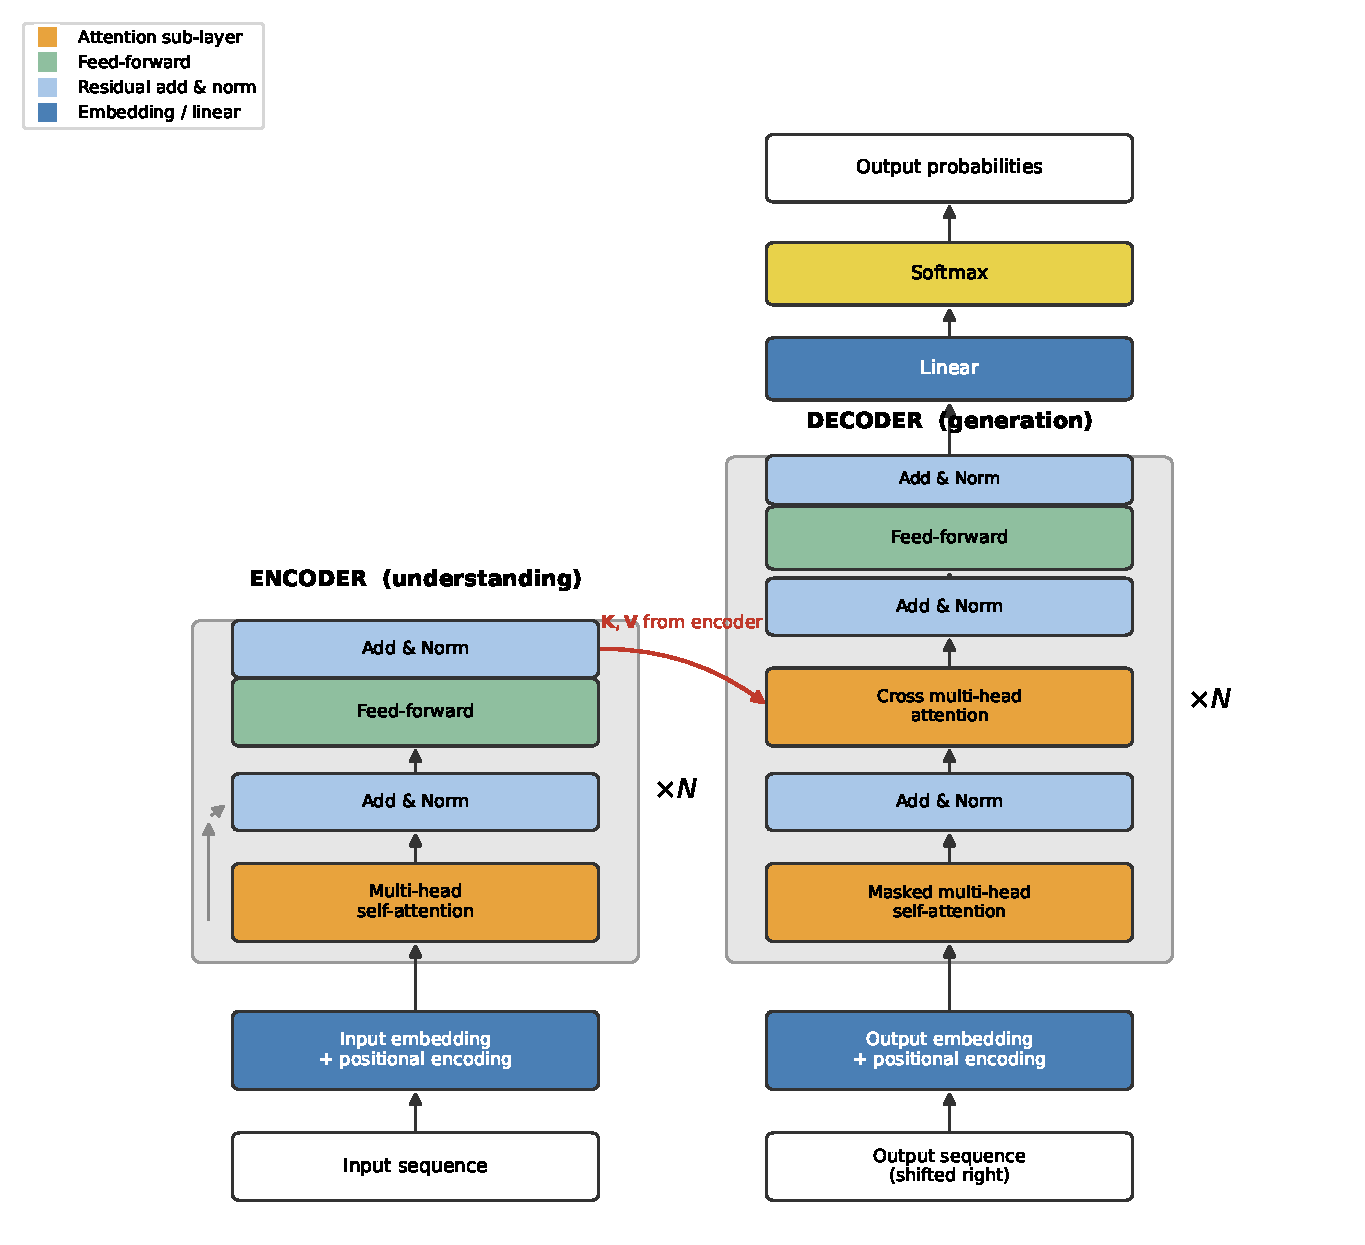
\includegraphics[width=0.7\linewidth]{files/figure_22_2_transfor-32e03fc756512304f5bc51ab8199c3b0.pdf}

FIGURE 22.2 makes the two data paths explicit. On the encoder side, each block applies multi-head self-attention followed by a feed-forward network, with every sub-layer wrapped in the residual add-and-normalise step of Equation (22.6), and the block is repeated N times. On the decoder side, an analogous stack inserts two extra pieces: a \textit{masked} self-attention, so that position $t$ cannot attend to tokens that come after it, and a \textit{cross-attention} sub-layer whose queries come from the decoder but whose keys and values come from the encoder output, which is how information flows from the input sequence to the generated one. A final linear projection followed by a softmax turns the top representation into a probability distribution over the vocabulary. The reader has met the words ``encoder'' and ``decoder'' before, in the autoencoder of Chapter 7, but the meaning here is different: the transformer's encoder and decoder do not compress and then reconstruct a single input, they map one sequence into another through attention.

We illustrate how self-attention resolves lexical ambiguity using a pre-trained transformer model.

\begin{verbatim}
from transformers import AutoTokenizer, AutoModel    # Hugging Face transformers
import torch

tokenizer = AutoTokenizer.from_pretrained('bert-base-uncased')
model = AutoModel.from_pretrained('bert-base-uncased',
                                  output_attentions=True)

sentences = [
    "The bank reported strong quarterly earnings.",   # Financial institution
    "We walked along the river bank at sunset.",      # River bank
]

for sent in sentences:
    inputs = tokenizer(sent, return_tensors='pt')
    with torch.no_grad():
        outputs = model(**inputs)
    # Extract embedding for "bank" token
    tokens = tokenizer.convert_ids_to_tokens(inputs['input_ids'][0])
    bank_idx = tokens.index('bank')
    embedding = outputs.last_hidden_state[0, bank_idx].numpy()
    print(f"'{sent}'")
    print(f"  'bank' at position {bank_idx}, "
          f"embedding norm: {np.linalg.norm(embedding):.3f}, "
          f"first 5 dims: {embedding[:5].round(3)}")
\end{verbatim}

\begin{verbatim}
'The bank reported strong quarterly earnings.'
  'bank' at position 2, embedding norm: 13.941, first 5 dims: [ 0.145 -0.421 -0.338  0.304  0.963]
'We walked along the river bank at sunset.'
  'bank' at position 6, embedding norm: 13.713, first 5 dims: [ 0.142 -0.66   0.029 -0.177 -0.21 ]
\end{verbatim}

The key observation is that the BERT embeddings for ``bank'' differ substantially between the two sentences, even though the word is identical. In the financial sentence, the embedding captures the meaning of ``bank'' as a financial institution (influenced by context words like ``earnings,'' ``quarterly,'' ``reported''). In the river sentence, the embedding reflects the geographical meaning (influenced by ``river,'' ``walked,'' ``sunset''). This is precisely the contextual understanding that static word embeddings (Chapter 21) cannot provide.

\begin{verbatim}
# Visualise attention pattern for the financial sentence
import matplotlib.pyplot as plt
inputs = tokenizer(sentences[0], return_tensors='pt')
with torch.no_grad():
    outputs = model(**inputs)

tokens = tokenizer.convert_ids_to_tokens(inputs['input_ids'][0])
attention = outputs.attentions[-1][0]                # Last layer, first head
attn_from_bank = attention[0, 2, :len(tokens)].numpy()  # Head 0, from "bank"

fig, ax = plt.subplots(figsize=(8, 4))
ax.bar(range(len(tokens)), attn_from_bank)
ax.set_xticks(range(len(tokens)))
ax.set_xticklabels(tokens, rotation=45, ha='right')
ax.set_ylabel('Attention weight')
ax.set_title("Attention from 'bank' to other tokens (last layer, head 0)")
plt.tight_layout()
plt.savefig('images/figure_22_1_bert_attention.png', dpi=140, bbox_inches='tight')
plt.show()
\end{verbatim}

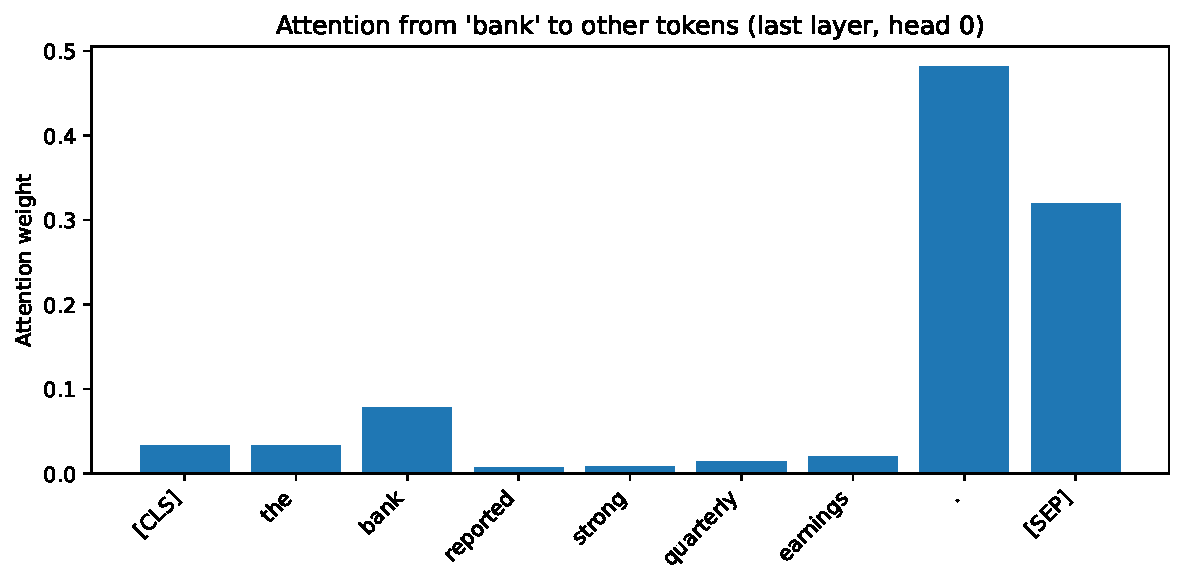
\includegraphics[width=0.7\linewidth]{files/figure_22_1_bert_att-ecea773b678058b459f5461fbc5aa46d.pdf}

As shown in FIGURE 22.1, the transformer concentrates attention from ``bank'' on the words ``earnings'' and ``reported,'' which disambiguate the financial meaning. This attention pattern demonstrates the mechanism by which transformers build contextual representations. As we discuss in Section 24.5, attention visualisation is also a useful interpretability tool for understanding what a model focuses on when making predictions.

\subsubsection{Architecture variants}

The original transformer of \cite{vaswani2017attention} contains both an encoder (which processes the input sequence) and a decoder (which generates the output sequence). Subsequent work has shown that using only the encoder or only the decoder yields powerful models for different tasks:

\begin{itemize}
\item \textbf{Encoder-only (BERT family).} The encoder processes the entire input sequence bidirectionally, meaning each token can attend to both left and right context. This is ideal for \textit{understanding} tasks: sentiment classification, named entity recognition, and textual similarity. BERT \citep{devlin2019bert} is the most prominent example.
\item \textbf{Decoder-only (GPT family).} The decoder processes tokens autoregressively, attending only to previous tokens (not future ones). This is ideal for \textit{generation} tasks: text completion, summarisation, and dialogue. GPT-2, GPT-3 \citep{brown2020language}, and subsequent models follow this paradigm.
\item \textbf{Encoder-decoder (T5, BART).} The full encoder-decoder architecture is used for \textit{sequence-to-sequence} tasks: translation, abstractive summarisation, and question answering. \cite{lewis2020bart} train BART as a denoising autoencoder in this family, and \cite{raffel2020exploring} showed that many NLP tasks can be framed in this text-to-text format.
\end{itemize}

The essential difference between the encoder-only and decoder-only families is not the depth of the stack but the \textit{attention mask} each one applies, illustrated in FIGURE 22.3.

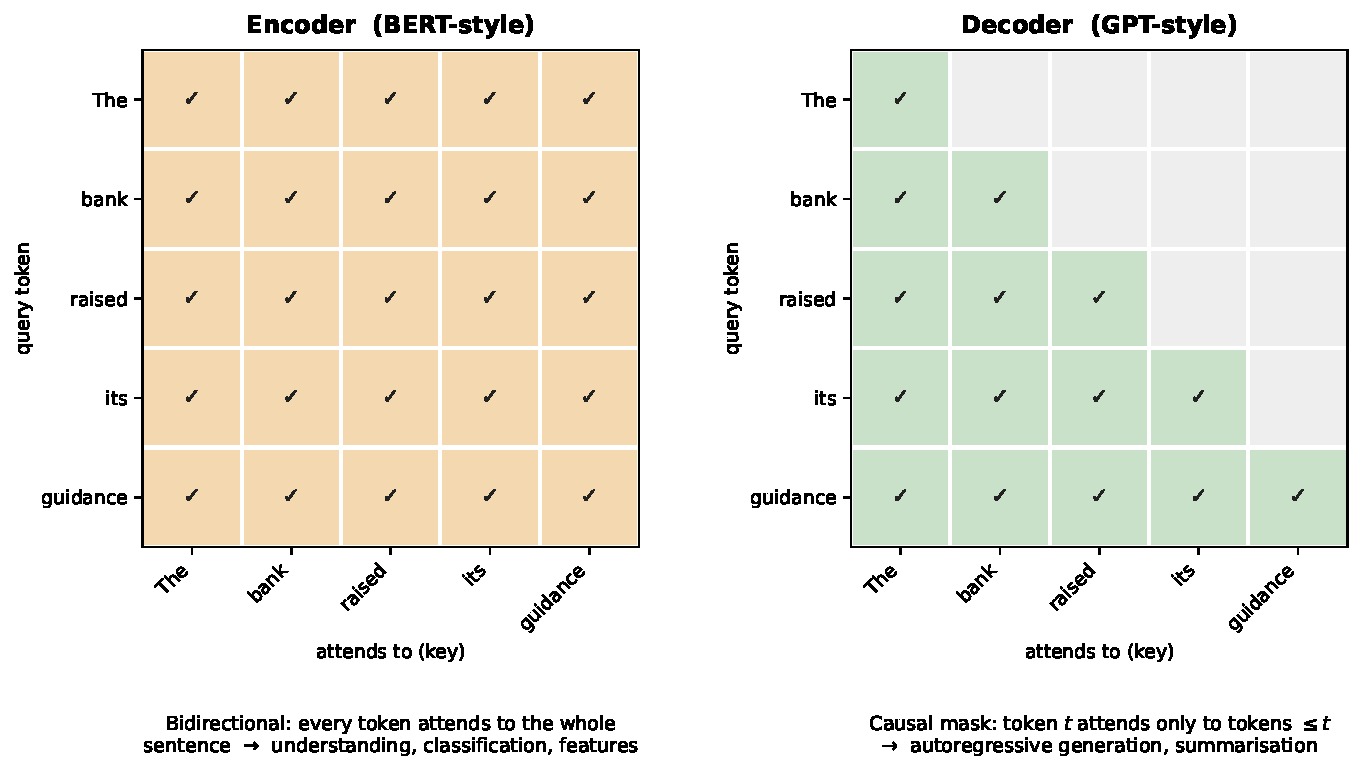
\includegraphics[width=0.7\linewidth]{files/figure_22_3_encoder_-b5ef1b82484dab5061b68639a352e06f.pdf}

The contrast in FIGURE 22.3 explains why the two families specialise as they do. Bidirectional attention lets an encoder condition each token's representation on the whole sentence, which is exactly what a sentiment classifier or a named-entity tagger needs, but it makes the model unusable for generation, since predicting the next word while already being allowed to see it is a degenerate task. The causal mask of the decoder removes that leakage, at the cost of context: each representation is built from the left only. For financial NLP, encoder-only models are most commonly used for classification and feature extraction, while decoder-only models (LLMs) are used for generation, summarisation, and zero-shot analysis. The encoder-only family is developed in the sections that follow; the decoder-only models that power large language models are the subject of Chapter 23.

\subsubsection{Transfer learning and fine-tuning}

Training a transformer from scratch requires enormous computational resources: BERT was pre-trained on 3.3 billion words (the entire English Wikipedia plus the BookCorpus) using 64 TPU chips for several days. Few financial practitioners have access to such resources. The solution is \textit{transfer learning}: pre-train a model on a large general-purpose corpus to learn the structure of language, then \textit{fine-tune} it on a small task-specific dataset to specialise it for the application of interest. \cite{howard2018ulmfit} established this pre-train-then-fine-tune paradigm for NLP text classification, showing that a language model pre-trained on general text could be adapted to a downstream task with only a modest labelled sample.

The pre-training phase teaches the model general linguistic knowledge: grammar, semantics, world knowledge, and reasoning patterns. The fine-tuning phase adapts this knowledge to a specific task (e.g., financial sentiment classification) using a much smaller labelled dataset, typically a few hundred to a few thousand examples. This approach works remarkably well because linguistic structure is largely shared across domains; what changes between general English and financial English is primarily vocabulary and domain-specific conventions.

\subsubsection{BERT and masked language modelling}

The value of bidirectional context had already been demonstrated by \cite{peters2018elmo}, whose ELMo model derived context-dependent word representations from a bidirectional LSTM language model; BERT brought this idea into the transformer. BERT (Bidirectional Encoder Representations from Transformers; \citep{devlin2019bert}) is pre-trained using two objectives:

\begin{enumerate}
\item \textbf{Masked language modelling (MLM).} Randomly select 15\% of the input tokens and train the model to predict them from context. In practice, of the selected positions, 80\% are replaced with a \texttt{[MASK]} token, 10\% with a random token, and 10\% are left unchanged, a scheme that reduces the mismatch between pre-training (which sees \texttt{[MASK]}) and fine-tuning (which does not). For example, given ``The [MASK] reported quarterly [MASK],'' the model must predict ``company'' and ``earnings.'' This forces the model to build rich bidirectional representations.
\item \textbf{Next sentence prediction (NSP).} Given two sentences concatenated with a \texttt{[SEP]} separator token, predict whether the second follows the first in the original text. This teaches the model about discourse coherence.
\end{enumerate}

Formally, let $\mathbf{x} = (x_1, \ldots, x_T)$ be an input token sequence and $\mathcal{M} \subset \{1, \ldots, T\}$ the random subset of masked positions (typically $|\mathcal{M}| = 0.15\, T$). The MLM objective is the masked negative log-likelihood,

\begin{equation}
\mathcal{L}_{\text{MLM}} = -\frac{1}{|\mathcal{M}|}\sum_{m \in \mathcal{M}} \log p_\theta(x_m \mid \mathbf{x}_{\setminus \mathcal{M}})
\tag{22.7}
\end{equation}

where $\mathbf{x}_{\setminus \mathcal{M}}$ denotes the input sequence with the positions in $\mathcal{M}$ replaced by a \texttt{[MASK]} token, and $\theta$ are the transformer parameters. The combined pre-training loss adds the binary next-sentence-prediction objective, $\mathcal{L}_{\text{BERT}} = \mathcal{L}_{\text{MLM}} + \mathcal{L}_{\text{NSP}}$. After pre-training, the model's internal representations (the output of the final transformer layer) serve as powerful features for downstream tasks. For classification, a simple linear layer is added on top of the \texttt{[CLS]} token embedding (a special token prepended to every input) and fine-tuned with labelled data.

\subsubsection{Finance-specific models}

General-purpose models like BERT sometimes struggle with financial text because of domain-specific vocabulary and conventions. Several finance-adapted models have been proposed:

\textbf{FinBERT} is in fact a family of three closely related models that are easily confused. The original \cite{araci2019finbert} version further pre-trained BERT on Reuters TRC2-financial news and fine-tuned it on the Financial PhraseBank sentiment benchmark. \cite{yang2020finbert} released a separate FinBERT trained from scratch on a much larger 4.9-billion-token corpus of corporate reports, earnings-call transcripts, and analyst reports, which has become the de facto open-source FinBERT in practitioner pipelines. \cite{huang2023finbert} then introduced a third FinBERT released alongside their \textit{Contemporary Accounting Research} paper, pre-trained on a still broader financial corpus and benchmarked on a wider battery of finance NLP tasks. All three significantly outperform general-purpose BERT and dictionary methods on financial sentiment benchmarks, and the differences between them matter mostly when reproducing prior numbers: the choice of pre-training corpus drives most of the residual gap.

\textbf{ClimateBERT} \citep{webersinke2022climatebert} is adapted for climate-related text, trained on climate disclosures, IPCC reports, and sustainability publications. It enables automated analysis of climate risk in corporate filings, a task of growing importance for ESG-oriented investors.

Domain adaptation is not confined to encoder models. \cite{wu2023bloomberggpt} train BloombergGPT, a decoder-only large language model, from scratch on a corpus that mixes financial and general-purpose text, producing a finance-specialised counterpart to the general generative models taken up in Chapter 23.

A parallel strand of research applies transformer architectures specifically to earnings-call transcripts, which pose a distinctive challenge because of their length (often thousands of tokens) and mixed register (formal prepared remarks followed by unscripted Q\&A). \cite{yang2020html} address this with HTML (Hierarchical Transformer-based Multi-task Learning), a model that segments a transcript into utterance-level blocks, applies a local transformer within each block, and then applies a second transformer across blocks to capture discourse-level structure. Trained jointly to predict both short-term volatility and price direction, HTML outperformed flat BERT and RNN baselines on earnings-call benchmarks, and it established the hierarchical transformer as the canonical architecture for long financial documents. The fact that the academic transcript literature \citep{yang2020html} and the practitioner transcript literature surveyed in Chapter 20 converge on the same genre of text underscores the importance of earnings calls as a signal source.

The common thread is \textit{domain adaptation}: starting from a general pre-trained model and further training on domain-specific text. This approach combines the linguistic knowledge from general pre-training with the specialised vocabulary and conventions of finance. It is worth emphasising a division of labour that the architecture motivates: these contextual encoder models excel at \textit{classification} tasks (sentiment, topic, entity type), where a single label is attached to the full input. For \textit{similarity} tasks across pairs of sentences or documents (peer-group construction, filing-change detection, cross-asset analogies), the sentence-transformer family of Section 21.4 is the more appropriate tool, because its contrastive training objective calibrates cosine distances in a way that the masked-language-modelling objective of standard BERT does not.

We apply FinBERT to the same six KO-flavoured sentences used in the Loughran-McDonald demonstration of Section 20.4 and compare its classifications directly against the dictionary approach.

\begin{verbatim}
from transformers import pipeline                    # High-level inference API

finbert = pipeline(
    'sentiment-analysis',
    model='ProsusAI/finbert',                        # Pre-trained FinBERT
    tokenizer='ProsusAI/finbert'
)

test_sentences = [                                   # the same six sentences scored in Section 20.4
    "Revenue growth was strong driven by innovation across our beverage portfolio.",
    "The softness in price mix was attributed to unfavorable category mix and constrained production capacity.",
    "Operating losses did not materialize, and margins held firm.",
    "Free cash flow improved and management sees favorable conditions for the remainder of the year.",
    "Adverse macroeconomic conditions and persistent inflation pose a risk to near-term consumer demand.",
    "The firm achieved outstanding results with superior margin expansion in North America.",
]

results = finbert(test_sentences)
for i, (sent, res) in enumerate(zip(test_sentences, results)):
    print(f"Doc {i}: {res['label']:>8s} ({res['score']:.3f})  {sent[:55]}...")
\end{verbatim}

\begin{verbatim}
Doc 0: positive (0.954)  Revenue growth was strong driven by innovation across o...
Doc 1: negative (0.950)  The softness in price mix was attributed to unfavorable...
Doc 2: positive (0.893)  Operating losses did not materialize, and margins held ...
Doc 3: positive (0.956)  Free cash flow improved and management sees favorable c...
Doc 4: negative (0.884)  Adverse macroeconomic conditions and persistent inflati...
Doc 5: positive (0.958)  The firm achieved outstanding results with superior mar...
\end{verbatim}

The contrast with the dictionary approach (Section 20.4) is striking. FinBERT correctly classifies Doc 2 (``Operating losses did not materialize, and margins held firm'') as positive with 89.3\% confidence, whereas the Loughran-McDonald dictionary scored it as -1.00. The model's contextual understanding of negation is its key advantage: it processes ``losses did not materialize'' as a single negated expression rather than counting ``losses'' in isolation.

\begin{verbatim}
# Compare FinBERT vs. dictionary on the same sentences
import pandas as pd
dict_scores = [1.0, -1.0, -1.0, 1.0, -1.0, 1.0]      # Loughran-McDonald net tone from Section 20.4
finbert_scores = [1.0 if r['label'] == 'positive'
                  else -1.0 if r['label'] == 'negative'
                  else 0.0 for r in results]

comparison = pd.DataFrame({
    'Dictionary': dict_scores,
    'FinBERT': finbert_scores,
    'Agree': [d * f > 0 for d, f in zip(dict_scores, finbert_scores)]
}, index=[f'Doc {i}' for i in range(len(dict_scores))])
print(comparison.to_string())
\end{verbatim}

\begin{verbatim}
Dictionary  FinBERT  Agree
Doc 0         1.0      1.0   True
Doc 1        -1.0     -1.0   True
Doc 2        -1.0      1.0  False
Doc 3         1.0      1.0   True
Doc 4        -1.0     -1.0   True
Doc 5         1.0      1.0   True
\end{verbatim}

The two methods agree on five of six sentences. The disagreement on Doc 2 highlights the negation-handling advantage of transformer-based models. In a large-scale evaluation this type of error correction accumulates, though the resulting lift over a well-tuned lexicon is typically modest.

\subsubsection{When to use FinBERT (and when not to)}

The practical gains of contextual representations are largest precisely for the failure modes catalogued in Section 20.4: negation, conditional language, and context-dependent polarity, cases in which the sentiment carried by a word depends on the words around it. Because FinBERT encodes each token in the context of the whole sentence rather than scoring it in isolation, it resolves many of the cases that a fixed lexicon systematically mishandles, and on standard financial-sentiment benchmarks it is usually the more accurate of the two. That advantage is genuine, but it is bounded, and it is worth being precise about where it stops.

Fine-tuned models are not a panacea. They require labelled training data, which is expensive to create for finance; they can be sensitive to the distribution of that data, so a model fine-tuned on news may underperform on earnings calls; and they are computationally heavier than dictionary lookups. For text that is relatively formulaic (standardised filings, for instance) and whose vocabulary is stable, dictionary methods remain a cost-effective baseline, a point the survey of textual analysis in accounting and finance by \cite{loughran2016textual} makes at length. More pointedly, FinBERT is no longer the frontier it once was: \cite{fatouros2023chatgpt} report that a general-purpose large language model (ChatGPT), simply prompted, outperforms FinBERT on financial-sentiment classification by roughly a third and correlates more strongly with subsequent returns, so the domain-specific fine-tune no longer dominates a general model that can be steered with a well-written prompt. A second and more unsettling line of criticism concerns robustness. \cite{leippold2023sentiment} shows that financial sentiment scores can be adversarially manipulated: paraphrasing a sentence with a language model flips a keyword classifier's verdict in close to 99\% of negative cases, and although context-aware encoders looked comparatively resistant in that study, \cite{turetken2026battle} go on to show that the transformer sentiment models themselves, FinBERT included, can be fooled by targeted attacks. The concern is not merely academic, since firms increasingly craft disclosures in the knowledge that machines will read them, so any deployed sentiment model operates in a setting where the very text it scores is partly written to move the score. The reasonable conclusion is not that FinBERT should be avoided, but that its output is one noisy, potentially gameable signal among several, best combined with dictionary and market-based measures rather than trusted on its own.

\subsubsection{Coding exercises}

\begin{enumerate}
\item Load a pre-trained FinBERT model with the \texttt{transformers} library and extract the
\texttt{[CLS]} token embedding for each of the six example sentences of Section 22.7.
Compute the pairwise cosine-similarity matrix of the embeddings, identify the pair
of sentences the model considers most similar, and comment on whether the grouping
reflects the topic of the sentences or their sentiment.
\end{enumerate}

\subsubsection{References}

\include{myst-chap-26-nlp-llms}

\subsection{End-to-end case study: building a text-based equity factor}

% 
% Version: 3.2.1
% Last updated: 2026-07-20
% Provenance: fifth and final chapter of Part V of the 2nd edition, extracted from
% the monolithic Chapter_20_Draft19.md (v3.9.7, archived in
% `_archive_monolithic_v3.9.7/`).
%

\subsubsection{Introduction}

Chapters 20 through 23 developed the four generations of NLP methods and the factor families each generation produces, but the empirical evaluations in those chapters were necessarily piecemeal: each method was demonstrated against the most natural baseline for its own paradigm, on the case-study universe but without the full portfolio-construction machinery that the book develops for traditional factor portfolios. This closing chapter of Part V brings the full pipeline together. We work through the practical considerations that every production text-factor pipeline must address, define the case study, construct features that span the methods of the preceding chapters, train and validate a model, run a backtest following the Chapter 12 protocol, and report the result in full, including the conditions under which the headline finding does and does not survive transaction costs.

The classical, embedding, transformer, and LLM methods of Chapters 20 through 23 are tools; the case study below shows what those tools produce when applied with discipline to the book's standard universe.

\subsubsection{Model selection and validation}

The choice of NLP model depends on the application, the available labeled data, and the computational budget. A useful hierarchy is:

\begin{enumerate}
\item \textbf{Dictionary methods} (Loughran-McDonald): fast, transparent, no training required. Suitable when the text is formulaic and the signal is well-understood.
\item \textbf{Fine-tuned BERT/FinBERT} (Chapter 22): moderate compute, requires labeled data. Best for classification tasks (sentiment, topic) where labeled examples are available.
\item \textbf{LLM with prompting} (Chapter 23): high compute, no training required. Best for complex tasks (summarization, reasoning, multi-label classification) or when labeled data is scarce.
\item \textbf{Fine-tuned LLM}: highest compute. Best when task-specific performance must be maximized and sufficient labeled data and compute are available.
\end{enumerate}

Validating NLP outputs for financial relevance requires more than standard ML metrics (accuracy, F1). A sentiment model might achieve 90\% accuracy on a benchmark dataset but produce signals with zero predictive power for returns. The ultimate validation is the out-of-sample portfolio performance of the resulting factor, not the NLP model's classification accuracy. For a broader methodological tour of this model hierarchy, from bag-of-words through learned classifiers and the validation traps specific to financial language, we refer the reader to the \textit{Journal of Accounting Research} survey of \cite{loughran2016textual}, which remains the most widely cited methodological reference in the area.

\subsubsection{Backtesting and timestamp discipline}

Backtesting NLP-based strategies introduces unique challenges beyond those discussed in Chapter 12.

\textbf{Timestamp discipline.} The most critical issue is \textit{look-ahead bias}. Financial text has a publication timestamp, and the NLP signal must be constructed using only information available at the time of portfolio formation. For example, a 10-K filing typically becomes available on EDGAR several weeks after the fiscal year end; using it as of the fiscal year end would introduce bias. News articles have precise timestamps, but the dissemination delay (time between event and publication) varies. Careful alignment of text timestamps with portfolio rebalancing dates is essential.

\textbf{Transaction costs and turnover.} NLP signals can be noisy, leading to high-turnover strategies that are eroded by transaction costs. Smoothing the signal (e.g., using a moving average of daily sentiment) or rebalancing at lower frequencies reduces turnover but may delay the incorporation of new information.

\textbf{Spanning tests.} A new NLP-derived signal is valuable when it adds information beyond the existing factor stack, and that value can be realised in more than one way: as a direct tilt in portfolio weights, as an input to stock selection, or as a filtering overlay that vetoes trades the base model would otherwise take, for example declining to short a name that carries strong short-term positive sentiment. The classic test for the first of these, the standalone-factor case, is the \textit{spanning regression}: we regress the NLP factor's long-short returns on a set of benchmark factors (for example the Fama-French five factors) and test whether the intercept (alpha) is significantly different from zero. A signal that is fully spanned adds no standalone alpha, but it may still earn its keep as a selection input or an overlay filter, which is exactly the distinction the case study of this chapter draws between adding sentiment as a feature and using it as a short-leg filter.

\subsubsection{Look-ahead bias and training-data leakage in LLM-based signals}

The timestamp discipline of Section 24.3 is the conventional anti-leakage hygiene: a signal at rebalance date $t$ may use only information actually released and indexed by $t$. For LLM-based signals, a second and more subtle form of leakage applies because the language model itself was pretrained on a corpus that almost certainly includes events that \textit{postdate} the historical sentences we are scoring. When we apply GPT-4 to a news headline from January 2018 and ask it to assess the tone for forward-return prediction, the model has, in principle, already read the news, the analyst commentary, and the eventual price reaction that followed; the resulting ``sentiment'' score may reflect that ex-post knowledge rather than the ex-ante linguistic cue. \cite{glasserman2023lookahead} named this concern \textit{look-ahead bias} and decomposed it into two distinct mechanisms. The first is \textit{specific} look-ahead bias, where the LLM has memorized the article-and-return pair and can effectively forecast the return from the headline alone. The second is a \textit{distraction effect}, where the LLM's general background knowledge about the named firm (it knows that Apple's iPhone 15 launched in September 2023, that SVB collapsed in March 2023, that NVIDIA dominated the 2024 AI capex cycle) colours the tone score independently of the headline's specific language. Their proposed test is an \textit{anonymization protocol}: replace every firm-name token in the headline with a generic placeholder, score the anonymized version, and compare returns. Surprisingly, on a US headline sample within the LLM training window they find that anonymized headlines \textit{outperform} unanonymized ones, indicating that the distraction effect is larger in magnitude than specific look-ahead bias. The implication for factor construction is direct: anonymization is not merely a debiasing step, it can in itself be an alpha-improving preprocessing step for LLM-based sentiment signals.

\cite{he2025chronologically} attack the problem from the other direction by training their own \textit{chronologically consistent} language models, ChronoBERT and ChronoGPT, which use only text published before each cutoff date. Their main finding is reassuring: when applied to a next-day-return prediction task on financial news, the ChronoBERT and ChronoGPT outputs achieve Sharpe ratios comparable to those of a much larger Llama model with no temporal restriction. The takeaway is that the \textit{magnitude} of look-ahead bias on standard sentiment-from-news tasks is modest provided that the downstream regression or classification head is properly retrained on a chronologically clean sample. The asset-pricing alpha attributed to LLM-derived sentiment in well-designed backtests therefore survives the leakage critique. The same paper also documents that chronological consistency is \textit{cheap} to maintain at inference time once the model has been pretrained with it; the marginal cost is incurred almost entirely at the pretraining stage.

Two more recent contributions confirm that the LLM-leakage risk is real, quantifiable, and operationally manageable. \cite{li2025profitmirage} coin the phrase \textit{profit mirage} for the gap between backtest performance and out-of-sample performance of LLM-based trading agents, reporting Sharpe ratio decay of 51 to 62 percent between in-sample and out-of-sample evaluation on their corpus, with the gap concentrated entirely in firms and time periods that the model is likely to have memorized. \cite{roy2026memguard} introduce \textit{MemGuard-Alpha}, a framework that combines five membership-inference-attack scores with cross-model disagreement (running the same prompt through multiple LLMs with different training cutoff dates and comparing the dispersion of their answers) to construct a signal-level \textit{contamination probability}. Filtering the strategy on the basis of that probability lifts the Sharpe ratio from 2.76 (unfiltered) to 4.11 (memorization-filtered), a 49 percent improvement, while \textit{clean} model signals produce 14.48 basis points of average daily return against 2.13 basis points for \textit{tainted} signals, a sevenfold ratio that is, if anything, more striking than the Sharpe number.

\textbf{Practical guidance for the LLM-sentiment factor.} Four steps suffice for the look-ahead-bias problem in the chapter's case study and in any production deployment that follows this pattern. First, \textit{anonymize firm identifiers} before scoring \citep{glasserman2023lookahead} so that the model cannot key its tone score on ex-post company-specific knowledge. Second, \textit{prefer chronologically consistent models} where available \citep{he2025chronologically}, and where the closed-frontier models must be used, restrict the evaluation window to dates strictly after the model's training cutoff. Third, \textit{cross-check across models with staggered training cutoffs} \citep{roy2026memguard} and flag any prompt whose answers diverge substantially across cutoffs as a likely contamination case. Fourth, \textit{report a profit-mirage diagnostic} alongside any backtest result: the ratio of out-of-sample Sharpe (post-cutoff) to in-sample Sharpe (pre-cutoff) is a useful single number, with values close to one indicating limited leakage and values far below one indicating that the reported backtest is partly an artefact of the language model's memorization. None of these steps is expensive, and together they take the chapter's empirical LLM-sentiment claims (the case study's long-short Sharpe improvement of Section 24.11, the high-regime advantage of TABLE 21.4) from being statistically reasonable to being defensible against the standard objections of the look-ahead-bias literature.

\subsubsection{Interpretability and compliance}

Regulatory requirements and investment mandates increasingly demand that a portfolio decision be explainable after the fact: a risk committee, an auditor, or a client may ask why a given name was held long or sold short, and ``the language model scored it positively'' is not, on its own, an acceptable answer. This requirement sits in direct tension with the modelling choices of the preceding chapters, because the most accurate text models (fine-tuned transformers and large language models) are also the least transparent. Three families of tools narrow the gap, and a text-factor pipeline intended for a regulated mandate should budget for all three.

\textbf{Token-level attribution.} Post-hoc attribution methods assign each input token a signed contribution to the model's output, turning an opaque score into a per-decision rationale. The workhorse is SHAP \citep{lundberg2017unified}, which computes Shapley-value attributions with game-theoretic consistency guarantees; for a financial sentiment prediction it might reveal that the word ``impairment'' contributes -0.3 to the score while ``growth'' contributes +0.2, giving a compliance officer a concrete, inspectable explanation. Two complementary methods are worth knowing. LIME \citep{ribeiro2016should} fits a sparse linear surrogate in the neighbourhood of a single prediction, and integrated gradients \citep{sundararajan2017axiomatic} attribute the prediction along a path from a baseline input to the actual input while satisfying a pair of axioms (sensitivity and implementation invariance) that ad-hoc saliency maps violate. For an audit trail, the axiomatic guarantees of integrated gradients and the consistency of SHAP are more defensible than a raw saliency heatmap.

\textbf{Attention and the faithfulness caveat.} Attention weights (Section 22.3) are the most readily available window into a transformer, showing which tokens the model attends to when it builds a representation, but they are a treacherous explanation. \cite{jain2019attention}, in ``Attention is not Explanation'', show that one can often construct very different attention distributions that leave the prediction unchanged, so a single attention map does not identify the tokens that were causally responsible. \cite{wiegreffe2019attention} reply, in ``Attention is not not Explanation'', that attention is not worthless either, provided the claim is tested against a properly constrained baseline rather than an unconstrained adversarial one. The practical lesson is that attention is a useful diagnostic and a poor legal defence: for a decision that must withstand scrutiny, it should be paired with an attribution method that carries formal guarantees.

\textbf{Finance-specific explainability.} The tools above are generic; their application to a regulated financial model has its own literature. \cite{bracke2019machine}, in a Bank of England staff working paper, apply Shapley-value explanations to a mortgage default-risk model and show how the resulting attributions can be organised into a regulator-facing account of which features drive a decision and how they interact. Their template, a global importance ranking together with local per-loan explanations and pairwise interaction effects, transfers directly to a text-derived factor: the same machinery that explains a default model can document which linguistic features move a sentiment factor, and is a natural starting point for the model-risk documentation that a text-factor strategy will require.

\textbf{LLM-specific risks: hallucination and auditability.} Large language models introduce a failure mode the attribution tools do not address: \textit{hallucination}, the generation of fluent but factually wrong statements, for example an invented revenue figure or a misattributed guidance change. For a signal that feeds real capital this is a first-order risk, and the mitigations are architectural rather than post-hoc: grounding the model in retrieved source documents (RAG, Section 23.7) so that every claim is traceable to a filing, attaching a confidence score and abstaining below a threshold, and inserting a human-in-the-loop checkpoint for high-stakes decisions. Two governance practices from the preceding chapter carry over directly. First, the reasoning trace of a tool-using agent (the ReAct-style thought-action-observation log of Section 23.11) is an auditable record that a compliance function can replay step by step. Second, reproducibility is itself a compliance control: pinning the decoding parameters (a low temperature and a fixed seed, Section 23.8), versioning the prompt, and logging every model call let a firm reconstruct exactly how a past decision was reached, which is what ``explain this trade'' ultimately requires.

\subsubsection{Frequency alignment: from quarterly text to monthly factors}

A practical question that the academic literature usually glosses over but that dominates production pipelines is this: the textual signals we have surveyed arrive at very different frequencies, ranging from annual 10-K filings to quarterly earnings transcripts to daily news flow to intra-day social-media posts, while the factor portfolio we want to construct typically rebalances at a single frequency, most often monthly or daily. The bridge between observation frequency and target frequency is not trivial, and the choice of bridge materially changes the empirical performance of the resulting factor. We catalogue the five canonical approaches found in the literature and in production practice.

\textbf{Persistence (forward-fill).} The simplest treatment carries the firm's most recent transcript signal $s_i(c)$ forward from the call date $t_c^i$ until the next call at $t_{c+1}^i$, so that $s_{i,t} = s_i(c)$ for all $t \in [t_c^i, t_{c+1}^i)$. The implicit assumption is that managerial tone evolves slowly between quarters. Several of the studies cited above adopt this convention implicitly by reporting firm-quarter signals as the firm's ``exposure'' for an entire quarter; \cite{sautner2023firm} and \cite{hassan2019politicalrisk} are representative. Forward-filling maximizes coverage but is fragile: it leaks look-ahead information if the transcript is not actually released until $t_c^i + \delta$ for some $\delta$, and it ignores the higher-frequency news flow that often updates the firm's narrative within the quarter.

\textbf{Exponential decay.} A second approach assumes that the influence of a transcript signal decays with calendar time, $s_{i,t} = s_i(c)\, e^{ -\lambda (t - t_c^i)}$, where $\lambda$ is calibrated so that the signal has a half-life $h = \ln 2 / \lambda$ in the range of a few weeks to a few months. Vendor pipelines routinely use exponential decay with $h$ of roughly 30 to 60 calendar days, calibrated empirically to match the decay of post-call return drift. The half-life choice is consequential: short half-lives (a week or two) effectively reduce the signal to an event-window indicator, while long half-lives (six months or more) approach pure forward-filling.

\textbf{Event-window treatment.} A third approach restricts the signal to a fixed event window, $s_{i,t} = s_i(c)$ for $t \in [t_c^i, t_c^i + N]$ and zero otherwise, where $N$ is typically 5, 21, or 63 trading days. This matches the event-study framing of \cite{tetlock2007giving}, \cite{tetlock2008more}, and \cite{bartov2018twitter}, and it isolates the announcement-period reaction from longer-horizon drift. Event-window treatment loses roughly three-quarters of observation-days relative to forward-filling, so it is best suited to questions about the announcement reaction itself rather than to building a continuously rebalanced factor portfolio.

\textbf{Rolling-window blending with daily news.} A fourth approach integrates the transcript signal into a higher-frequency rolling estimator over news. Hafez and Xie (2012, 2014) construct firm-level sentiment indices from a moving 90-day window over news flows in which the quarterly earnings call is one observation among many feeding the rolling estimator. The rolling window naturally smooths across the transcript-and-news boundary, and \cite{hafez2021transcripts} document that overlaying transcripts on a news-only base materially improves the cross-sectional information ratio at horizons of a few days to a week. The blending approach is the one we recommend as the default in production: it preserves the quarterly anchor while letting daily news supply the intra-quarter innovations.

\textbf{Quarterly resampling.} A fifth and most conservative approach is to resample everything to firm-quarter frequency and avoid the alignment problem altogether. This is appropriate when the target portfolio rebalances quarterly anyway, which is the case for several slow-style implementations of the factors of Chapter 3. The cost is a coarse picture of timing; the benefit is that no temporal extrapolation is required.

\textbf{Practical guidance.} The choice among these five reduces to two empirical questions. First, what is the actual half-life of the signal under study? Slow-moving signals such as managerial confidence \citep{kim2024transcripts}, political risk \citep{hassan2019politicalrisk}, and climate exposure \citep{sautner2023firm} plausibly persist for months and forgive forward-filling. Fast-moving signals such as guidance-surprise tone or analyst-question stress decay over days to weeks and require either exponential decay or an event window. Second, is daily news available for the same firm? When the answer is yes, blending the transcript anchor with the higher-frequency news stream dominates pure persistence or pure decay because the news stream supplies the intra-quarter updates that the transcript cannot. As a special case worth flagging, the annual-filings literature exemplified by \cite{cohen2020lazy} has an even worse frequency mismatch (one observation per year against a monthly target); the convention there is to treat the year-over-year textual change as an ``active'' signal for the twelve months after the filing date, which is essentially the forward-fill convention adapted to an annual cadence. Whichever bridge is chosen, it must respect the timestamp discipline of Section 24.3: the signal at portfolio rebalance date $t$ may use only information actually released and indexed by $t$, not the headline date printed on the call.

\subsubsection{Computational cost}

The computational requirements of NLP methods span several orders of magnitude, as we summarize in TABLE 24.1.

\textbf{TABLE 24.1: Approximate computational costs for different NLP methods applied to a single financial document.} Latencies are order-of-magnitude estimates on standard hardware; cost categories combine compute, memory, and (for API-served LLMs) per-token pricing.

\bigskip\noindent
\begin{tabular}{p{\dimexpr 0.333\linewidth-2\tabcolsep}p{\dimexpr 0.333\linewidth-2\tabcolsep}p{\dimexpr 0.333\linewidth-2\tabcolsep}}
\toprule
Method & Typical latency per document & Cost profile \\
\hline
Dictionary lookup & \textless  1 ms & Negligible \\
TF-IDF + sklearn classifier & \textless  10 ms & Negligible \\
spaCy NER & {\textasciitilde}50 ms & Low \\
BERT/FinBERT inference & {\textasciitilde}100 ms (GPU) & Moderate \\
LLM inference (API) & {\textasciitilde}1-5 s & High (per-token pricing) \\
LLM fine-tuning & Hours to days & Very high \\
\bottomrule
\end{tabular}

\bigskip

For a universe of 1,000 stocks with monthly rebalancing and one document per stock per month, dictionary methods process the entire corpus in seconds, FinBERT requires minutes (on a GPU), and LLM API calls require hours and incur non-trivial monetary costs. The cost-benefit analysis depends on the fund size: the marginal alpha from LLM-based signals may justify the cost for a large quantitative fund but not for a small portfolio.

Parameter-efficient fine-tuning techniques such as LoRA and QLoRA (see Section 23.5) reduce the memory and compute requirements of LLM adaptation by one to three orders of magnitude relative to full fine-tuning, making on-premise domain specialization accessible to teams without data-center GPU fleets.

\subsubsection{Problem statement and hypothesis}

We now bring together the techniques from this chapter in a structured case study. The question is simple: \textit{can NLP-derived features improve the predictive performance of the factor models?}

Our hypothesis is that sentiment signals, constructed from financial text, contain information about future returns that is not fully captured by the numerical characteristics in the book's dataset.

A useful real-world precedent is the study of \cite{kangrga2020factor}, who built a long-short market-neutral sentiment factor for the Asia-Pacific ex-Japan mid- and large-cap universe (around 900 names from 2007 to 2020) using a commercial event-level sentiment feed, a 60-day smoothing window, and a novelty filter that retains only the first occurrence of each event within the prior 90 days. Their standalone sentiment factor delivered an annualized return above 400 basis points with an information ratio above 0.7, even at monthly rebalancing, and exhibited essentially zero correlation with the six traditional style factors (Momentum, Low Size, Low Volatility, Growth, Value, Quality) constructed on the same universe. When the sentiment factor was added to a multi-factor portfolio combining the six traditional styles, the information ratio rose from 0.45 to 0.74 and the annualized return from 167 to 225 basis points, with only a moderate increase in turnover. The academic literature reaches the same conclusion from independent samples and cleaner identification. \cite{heston2017news} construct a news-tone factor that is positively correlated with, but not subsumed by, price momentum, so that combining the two raises the Sharpe ratio of the pair; \cite{ke2019predicting} show that a supervised sentiment score extracted from news text predicts the cross-section of returns net of the standard risk factors; and \cite{calomiris2019news} document that news-based measures carry return- and risk-relevant information across a broad international cross-section. Two design choices stand out from Hafez et al.'s methodology and inform our case study below: aggressive novelty and relevance filtering (only events scoring at least 90 on the vendor's relevance and similarity-day filters are retained), and the construction of the factor as an \textit{orthogonal} alternative source of risk premium rather than as an overlay on existing factors.

The intuition is straightforward. A sentiment factor that is genuinely orthogonal to the existing style factors adds return without adding proportional variance, so the information ratio of the combination exceeds that of the style factors alone. This is precisely the additivity that \cite{kangrga2020factor} document empirically, and it is the property we now test on the book's standard dataset.

\subsubsection{Data and feature construction}

In a complete implementation, the workflow is:

\begin{enumerate}
\item For each stock-month pair in the dataset, retrieve all relevant text documents (10-K/10-Q filings, news articles, earnings call transcripts) published during the prior month.
\item Apply a sentiment model (dictionary, FinBERT, or LLM) to each document to obtain a raw sentiment score.
\item Aggregate scores to the stock-month level (e.g., average sentiment weighted by recency).
\item Uniformize the sentiment feature cross-sectionally at each date to match the convention of Chapter 4.
\item Merge with the existing dataset.
\end{enumerate}

The chapter's case-study pipeline executes exactly this workflow for earnings-call transcripts: the NLP US universe across 83 quarters (2005-2026) that anchors TABLE 21.1 of Section 21.7, three speech buckets per call (prepared-mgmt, Q\&A-mgmt, Q\&A-analyst), scored by Llama-3.1-8B on four orthogonal dimensions (managerial confidence, specificity, surprise-negative, macro-vs-firm risk framing), with an explicit cross-sectional anchor (Section 23.8). Three real NLP features are extracted from this pipeline.

We first build the case-study \texttt{panel} by merging the numerical dataset with the earnings-call scores. FinBERT and LM contribute their prepared-remarks tone directly; the LLM contributes the signed four-axis composite (managerial confidence plus specificity minus surprise-negative plus macro-versus-firm framing, averaged over the three speech buckets). Each quarterly call is broadcast to the monthly grid with a one-quarter carry (a 110-day stale-out, matching the quarterly call cadence with a small buffer).

\begin{verbatim}
import pandas as pd, numpy as np
ml = pd.read_parquet('mlfi_us_data.parquet').sort_values(['id', 'date'])   # monthly id x date
sw = pd.read_parquet('sentiment_panel.parquet')                            # one row per call, with id
ml['date'] = ml['date'].astype('datetime64[ns]')          # align dtypes for the as-of merge
sw['date'] = sw['date'].astype('datetime64[ns]')

sw['s_finbert'] = sw['finbert_prep_mgmt']                  # FinBERT prepared-remarks tone
sw['s_lm']      = sw['lm_tone_prep_mgmt']                  # LM net tone, prepared remarks
buckets = ['prep_mgmt', 'qa_mgmt', 'qa_analyst']           # signed 4-axis LLM score per bucket
per_bucket = [(sw[f'llm_managerial_confidence_{b}'] + sw[f'llm_specificity_{b}']
               - sw[f'llm_surprise_negative_{b}'] + sw[f'llm_macro_vs_firm_risk_framing_{b}']) / 4
              for b in buckets]
sw['s_llm_4d'] = pd.concat(per_bucket, axis=1).mean(axis=1)   # composite over the three buckets

calls = (sw.dropna(subset=['id']).astype({'id': 'int'})
           [['id', 'date', 's_llm_4d', 's_finbert', 's_lm']].sort_values('date'))
panel = ml.merge(pd.merge_asof(ml[['id', 'date']].sort_values('date'), calls,   # <=110-day carry
                               on='date', by='id', direction='backward',
                               tolerance=pd.Timedelta('110D')),
                 on=['id', 'date'], how='left')
panel = panel[panel['R1M_Usd'].notna()].copy()             # need the forward return observed
\end{verbatim}

We then uniformize the three sentiment features cross-sectionally at each date, matching the convention of Chapter 4.

\begin{verbatim}
panel['s_llm_4d_r']  = panel.groupby('date')['s_llm_4d'].transform(
    lambda x: x.rank(pct=True))                     # LLM 4-dim composite
panel['s_finbert_r'] = panel.groupby('date')['s_finbert'].transform(
    lambda x: x.rank(pct=True))                     # FinBERT prep-mgmt tone
panel['s_lm_r']      = panel.groupby('date')['s_lm'].transform(
    lambda x: x.rank(pct=True))                     # LM net tone, prep-mgmt

nlp_features = ['s_llm_4d_r', 's_finbert_r', 's_lm_r']
print(f"NLP features: {nlp_features}")
print(panel[nlp_features].describe().round(3).to_string())
\end{verbatim}

\begin{verbatim}
s_llm_4d_r  s_finbert_r  s_lm_r
count   83078.000    79551.000  79553.000
mean        0.501        0.502      0.502
std         0.289        0.289      0.288
min         0.002        0.002      0.002
25%         0.251        0.250      0.254
50%         0.501        0.501      0.500
75%         0.751        0.751      0.751
max         1.000        1.000      1.000
\end{verbatim}

The three real NLP features are uniformized to $[0, 1]$ and have the same distributional shape as the existing features, ensuring comparability. Coverage is 83,078 stock-months for the LLM composite, set by the intersection of the LLM-pipeline coverage (the NLP US universe of TABLE 21.1) and the \texttt{mlfi\_us\_data} universe match; the LLM-covered tickers that fall outside the book's standard panel are dropped at the merge step. The FinBERT and LM features have slightly smaller coverage (79,551 stock-months) because the underlying transcript-level FinBERT and LM tone scores are missing on a small subset of calls where the prepared-remarks bucket failed to split cleanly. The case study below restricts to the LLM-covered slice so that the predictive evaluation isolates the sentiment contribution rather than measuring the noise of filling missing rows with a neutral default; the small FinBERT/LM gap is handled by the median-by-date imputation already applied to the base features.

\subsubsection{Model training and evaluation}

We train gradient-boosted tree models with and without the NLP features, following the protocol of Chapter 6. For simplicity, and to keep the worked example quick to run and reproduce, the case study fits a single \textit{static} model: we train once on all data before the chronological separation date and score the entire out-of-sample period with that one fitted model, rather than the expanding-window, periodically-retrained walk-forward of Section 21.7.4. The static split keeps the pipeline legible at the cost of not letting the model adapt to post-separation regime shifts; a walk-forward re-run, refitting as new data arrives, is a natural robustness extension, in the same spirit as the chronologically-consistent replication flagged in Section 24.4.

\begin{verbatim}
features = [c for c in ml.columns                    # the 122 base mlfi_us_data characteristics
            if c not in ['id', 'date', 'R1M_Usd', 'R3M_Usd', 'R6M_Usd', 'R12M_Usd']]
separation_date = pd.Timestamp('2014-01-15')         # chronological train/test split

features_base = sorted([c for c in features         # every usable characteristic
                         if panel[c].isna().mean() < 0.05])
features_all  = features_base + nlp_features        # all characteristics + 3 NLP

for c in features_base:                              # impute remaining NaNs
    panel[c] = panel.groupby('date')[c].transform(lambda x: x.fillna(x.median()))
training = panel[panel['date'] < separation_date]
testing  = panel[panel['date'] >= separation_date]

X_train_base, X_test_base = training[features_base], testing[features_base]
X_train_all,  X_test_all  = training[features_all],  testing[features_all]
y_train, y_test = training['R1M_Usd'], testing['R1M_Usd']

import xgboost as xgb
params = dict(
    n_estimators=100, max_depth=4,
    learning_rate=0.1, subsample=0.8,
    colsample_bytree=0.8, random_state=42
)

fit_base = xgb.XGBRegressor(**params).fit(X_train_base, y_train)
fit_all  = xgb.XGBRegressor(**params).fit(X_train_all, y_train)

pred_base = fit_base.predict(X_test_base)
pred_all  = fit_all.predict(X_test_all)
\end{verbatim}

\begin{verbatim}
from scipy.stats import spearmanr
from sklearn.metrics import mean_squared_error

mse_base = mean_squared_error(y_test, pred_base)
mse_all  = mean_squared_error(y_test, pred_all)
hr_base  = np.mean(np.sign(y_test) == np.sign(pred_base))
hr_all   = np.mean(np.sign(y_test) == np.sign(pred_all))
ic_base, _ = spearmanr(y_test, pred_base)
ic_all,  _ = spearmanr(y_test, pred_all)

results_df = pd.DataFrame({
    'Metric': ['MSE', 'Hit ratio', 'IC (Spearman)'],
    'all base':    [f'{mse_base:.6f}', f'{hr_base:.4f}', f'{ic_base:+.4f}'],
    'all + 3 NLP': [f'{mse_all:.6f}',  f'{hr_all:.4f}',  f'{ic_all:+.4f}'],
})
print(results_df.to_string(index=False))
\end{verbatim}

\begin{verbatim}
Metric  all base  all + 3 NLP
           MSE  0.014842     0.014872
     Hit ratio    0.5333       0.5351
IC (Spearman)   +0.0060      +0.0120
\end{verbatim}

Adding the three NLP features to the full 122-characteristic base leaves the squared-error fit essentially untouched (the mean squared error is flat, edging marginally higher from 0.014842 to 0.014872) but lifts the two rank-based metrics: the cross-sectional information coefficient roughly doubles, from +0.0060 to +0.0120, and the hit ratio rises from 53.3\% to 53.5\%. That split is the central lesson of the exercise. Averaged over a full month, in which the post-call signal has largely decayed and the characteristic stack already explains most of the magnitude variation, an incremental text feature adds nothing to a symmetric squared-error objective; but the same feature still sharpens the model's \textit{ordering} of the cross-section, which is what a rank correlation measures and what a long-short portfolio acts on. The pooled regression and the tail-sort therefore look at different things, and the backtest of the next section shows that the ordering improvement is where the economic value lives.

The reconciliation is that squared error accumulates in the bulk of the distribution, which the base characteristics already dominate, while the sentiment features earn their keep at the extremes, among the most and least favoured names, exactly where a quintile long-short operates. The 5-day-horizon results of TABLE 21.1 make the same point more sharply, with the LLM composite earning a clean cross-sectional IC of 0.19 and an IR above 2 against forward-five-day returns; at the monthly rebalance the effect is muted but, as the doubled rank-IC already hints, not absent. The empirical evidence \citep{ke2019predicting, kim2024transcripts} reaches the same conclusion, that real NLP features do add value, particularly for sentiment and forward-looking information, and that the value is largest when the rebalance frequency matches the information horizon (the frequency-alignment discussion of Section 24.6).

\subsubsection{Portfolio backtest}

We follow the portfolio construction protocol of Chapter 12 to evaluate the economic impact of adding the NLP features. The first thing to recall is the return convention: at each row \texttt{date = t} of \texttt{mlfi\_us\_data}, the label \texttt{R1M\_Usd} is the \textit{forward} one-month return realised between $t$ and $t + 1$ month, so a portfolio formed at month-end $t$ using predictions made from features observed at $t$ realises \texttt{R1M\_Usd[t]} over the subsequent month. We therefore use \texttt{R1M\_Usd} directly as the realised return of the formed portfolio, and we compound monthly rather than simply averaging cross-sectional means.

At each month-end we sort the test-set stocks by model-predicted next-month return, take the top quintile as the long leg and the bottom quintile as the short leg, equal-weight within each leg, and record the long-short monthly return alongside the leg-level turnover (the fraction of names rotating in or out of each leg from one month to the next, which we report as a gauge of each strategy's trading intensity and its exposure to transaction costs).

We evaluate three portfolios. The \textit{base} strategy sorts on the all-characteristics model of the preceding section; the \textit{NLP-feature} strategy sorts on the model that also sees the three sentiment features; and a third, \textit{sentiment-filter} strategy uses the LLM sentiment composite not as a model input but as an overlay on the base book. The idea is the smart middle ground between ignoring sentiment and rebuilding the model around it: we take the base model's long and short quintiles and then refuse to short any name whose LLM sentiment composite is strongly positive, and refuse to go long any name whose composite is strongly negative, dropping the roughly one-third of each leg that most conflicts with the sentiment reading. Sentiment here corrects the characteristic model's most dangerous positions, a fundamentally-cheap stock the market is enthusiastic about, or a fundamentally-expensive one it has soured on, rather than trying to add marginal signal everywhere. Using sentiment as an overlay rather than as a primary signal has precedent in both the practitioner and the academic literature: \cite{uhl2015news} drive a tactical allocation from news-sentiment momentum used as an overlay, \cite{hafez2014web} overlay news sentiment on a short-term reversal strategy and raise its information ratio by up to 70\%, and \cite{stambaugh2012short} show that sentiment-driven mispricing concentrates in the short leg of anomaly strategies, precisely the leg our filter screens most aggressively.

\begin{verbatim}
def build_ls(df, pred, sent=None):                    # one row per month; sent = filter column
    rows, prev_long, prev_short = [], set(), set()
    for d, g in df.sort_values('date').groupby('date'):
        if len(g) < 10: continue
        longs  = g[g[pred] >= g[pred].quantile(0.80)]
        shorts = g[g[pred] <= g[pred].quantile(0.20)]
        if sent:                                       # sentiment filter (the "medium" strategy)
            longs  = longs[longs[sent]  >= 0.34]       # do not go long a strongly-negative name
            shorts = shorts[shorts[sent] <= 0.66]      # do not short a strongly-positive name
        long_ids, short_ids = set(longs['id']), set(shorts['id'])
        if not long_ids or not short_ids: continue
        r_long, r_short = longs['R1M_Usd'].mean(), shorts['R1M_Usd'].mean()   # eq-weight legs
        turn_l = 1 - len(long_ids  & prev_long)  / max(len(prev_long),  1) if prev_long  else np.nan
        turn_s = 1 - len(short_ids & prev_short) / max(len(prev_short), 1) if prev_short else np.nan
        rows.append(dict(date=d, r_ls=r_long-r_short, turn_l=turn_l, turn_s=turn_s))
        prev_long, prev_short = long_ids, short_ids
    return pd.DataFrame(rows)

testing_data = testing[['date','id','R1M_Usd','s_llm_4d_r']].copy()
testing_data['pred_base'] = pred_base
testing_data['pred_all']  = pred_all
ls_base   = build_ls(testing_data, 'pred_base')
ls_all    = build_ls(testing_data, 'pred_all')
ls_filter = build_ls(testing_data, 'pred_base', sent='s_llm_4d_r')   # base model, filtered book
\end{verbatim}

\begin{verbatim}
def perf_stats(ls, cost_bps=0):                       # MLFI Ch. 12 style block
    r = ls.r_ls.values.copy()
    if cost_bps:                                       # round-trip cost per leg
        r -= (ls.turn_l.fillna(0).values + ls.turn_s.fillna(0).values) * cost_bps/1e4
    wealth = (1 + r).cumprod()
    cagr   = wealth[-1]**(12/len(r)) - 1
    ann_vol, sharpe = r.std(ddof=1)*np.sqrt(12), r.mean()*12/(r.std(ddof=1)*np.sqrt(12))
    mdd    = (wealth / np.maximum.accumulate(wealth) - 1).min()
    return dict(CAGR=cagr, AnnVol=ann_vol, Sharpe=sharpe, MaxDD=mdd,
                Calmar=cagr/abs(mdd), Hit=(r>0).mean(), t_stat=r.mean()/(r.std(ddof=1)/np.sqrt(len(r))),
                AvgTurnPerLeg=(ls.turn_l.mean()+ls.turn_s.mean())/2, FinalWealth=wealth[-1])

cols = ['CAGR','AnnVol','Sharpe','MaxDD','Calmar','Hit','t_stat','AvgTurnPerLeg','FinalWealth']
rows = {'all base':               perf_stats(ls_base),        # gross long-short statistics
        'all + 3 NLP':            perf_stats(ls_all),
        'all + sentiment filter': perf_stats(ls_filter)}
print(pd.DataFrame(rows).T[cols].round(3).to_string())
\end{verbatim}

\begin{verbatim}
CAGR  AnnVol  Sharpe  MaxDD  Calmar    Hit  t_stat  AvgTurnPerLeg  FinalWealth
all base                0.072   0.133   0.586 -0.193   0.373  0.562   2.045          0.427        2.327
all + 3 NLP             0.077   0.128   0.643 -0.178   0.434  0.527   2.242          0.457        2.472
all + sentiment filter  0.139   0.145   0.967 -0.251   0.552  0.534   3.374          0.498        4.854
\end{verbatim}

Three observations follow from the stat block. First, on a gross basis both sentiment treatments improve the base portfolio, and the filter improves it dramatically. The long-short Sharpe rises from 0.59 (base) to 0.64 with the NLP features and to 0.97 with the sentiment filter; the filter also posts by far the highest annualised return (13.9\% against 7.2\% for the base and 7.7\% for the NLP-feature version) and the largest terminal wealth (4.85 dollars per dollar invested, against 2.33 for the base and 2.47 for the NLP version). Interestingly, the base model keeps the highest monthly hit ratio (56.2\% against 52.7\% for the NLP version and 53.4\% for the filter), so the overlays win through the \textit{size} of their favourable months rather than their frequency, trading a slightly lower win rate for materially larger average wins. The filter earns its edge by construction: refusing to short strongly-positive-sentiment names and to hold long strongly-negative ones removes exactly the positions most prone to being run over by news, concentrating the book in the names where the characteristic ranking and the sentiment reading agree. That the long-short results improve while the pooled monthly regression of the preceding section barely moved is the reconciliation promised above: the backtest acts only on the top and bottom quintiles, exactly where sentiment either sharpens the ranking (the doubled rank-IC of the previous section) or vetoes a dangerous position, whereas the pooled squared-error fit is dominated by the bulk of the cross-section that the base characteristics already explain.

Second, the two overlays reshape risk in opposite directions. The NLP-feature model earns its modest gain while slightly reducing risk, with the maximum drawdown easing from -19.3\% (base) to -17.8\% and volatility from 13.3\% to 12.8\%, so its Calmar ratio improves from 0.37 to 0.43. The sentiment filter takes the opposite trade: it runs a higher volatility (14.5\%) and a deeper maximum drawdown (-25.1\%) than the base, but more than compensates with return, so its Calmar still rises to 0.55 and its Sharpe to 0.97. Concentrating the book raises both its upside and its tail risk. On a calendar-year basis the NLP-feature version beats the base in five of the twelve years and the filter in eight of the twelve.

Third, and most soberingly, these are \textit{gross} figures, and the full 122-characteristic model trades heavily: average turnover is roughly 43\% per leg for the base, 46\% for the NLP-feature portfolio, and 50\% for the sentiment filter, several times the turnover of a compact model, because a richer model reshuffles the marginal-quintile names far more often. Realistic transaction costs would therefore erode a material share of every advantage reported above, and the filter's higher turnover makes it the most cost-sensitive of the three, which bites hardest precisely because it also carries the largest gross edge. We deliberately do not attach a single net-of-cost number, because any such figure depends on the execution venue, the borrow cost of the short leg, and the rebalancing discipline, none of which is pinned down on this universe. The defensible claim is that the gross ordering (filter well above NLP-feature above base) is clear, and that how much of it survives in practice is decided by turnover management, through the signal-smoothing and transaction-cost-aware construction of Chapter 12 \citep{martin2018transaction}.

A graphical summary of the strategy follows the convention of Section 12.6: a cumulative-wealth curve and a yearly performance bar chart, both constructed from the monthly long-short return series above.

\begin{verbatim}
import matplotlib.pyplot as plt                                    # plotting backend
wealth = pd.DataFrame({                                            # cumulative-wealth frame
    'base':          (1 + ls_base.set_index('date').r_ls).cumprod(),    # base model NAV
    'base + NLP':    (1 + ls_all.set_index('date').r_ls).cumprod(),     # NLP-feature NAV
    'base + filter': (1 + ls_filter.set_index('date').r_ls).cumprod()}) # sentiment-filter NAV
wealth.index = pd.to_datetime(wealth.index)                        # ensure datetime index
ye     = wealth.resample('YE').last()                              # year-end NAV
yearly = ye.pct_change().dropna()                                  # year-on-year return
yearly.index = yearly.index.year                                   # integer years for bars

palette = ['#444444', '#cc3333', '#2a7fbf']                        # base / NLP / filter
fig, (ax1, ax2) = plt.subplots(1, 2, figsize=(14, 4.5))            # 2-panel layout
wealth.plot(ax=ax1, lw=1.6, color=palette)                         # wealth curves, left
ax1.set_title('Cumulative wealth (LS portfolio, gross)')           # left title
ax1.set_ylabel('Cumulated value'); ax1.grid(True, alpha=.3)        # axis + grid
yearly.plot.bar(ax=ax2, color=palette, width=0.8)                  # yearly bars, right
ax2.set_title('Yearly performance (LS portfolio, gross)')          # right title
ax2.set_ylabel('Annual return')                                    # axis label
ax2.axhline(0, color='black', lw=0.5)                              # zero line
ax2.grid(True, alpha=.3, axis='y')                                 # horizontal grid only
ax2.yaxis.set_major_formatter(plt.FuncFormatter(                   # percent ticks
    lambda y,_: f'{y:.0%}'))
plt.tight_layout()                                                 # avoid overlap
plt.savefig('images/figure_24_1_case_backtest.png', dpi=130)     # persist figure
\end{verbatim}

FIGURE 24.1 shows the resulting two panels.

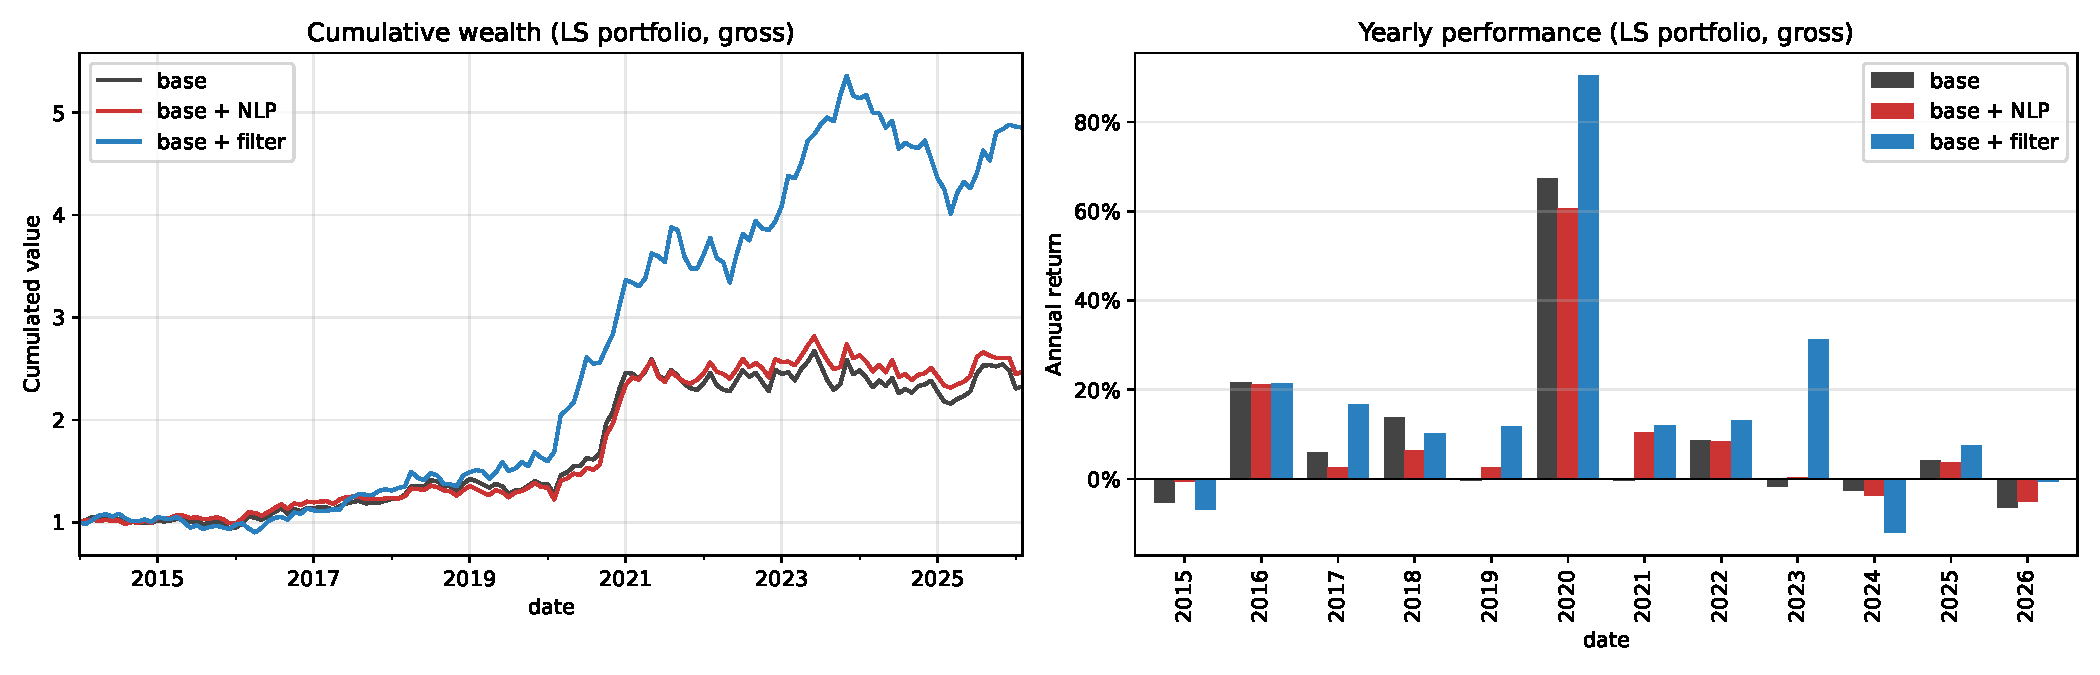
\includegraphics[width=0.7\linewidth]{files/figure_24_1_case_bac-6d7eaa395c4431da788beac29c5d8959.pdf}

The left panel of FIGURE 24.1 plots the cumulative wealth of one dollar invested in each long-short portfolio from January 2014 to the end of the test sample, gross of transaction costs. All three strategies rest on the full 122-characteristic base model; the NLP-feature strategy adds the three real NLP features (LLM 4-dim composite, FinBERT prepared-remarks tone, LM net tone) to the model, while the sentiment-filter strategy overlays the LLM composite on the base book. One dollar grew to 2.33 in the base strategy, 2.47 with the NLP features, and 4.85 with the sentiment filter over the same window, the filter's lead built largely in a handful of strong years (2017, 2019, 2020, and 2023). The right panel decomposes each wealth path into year-on-year performance by reading year-end NAV; the NLP-feature version beats the base in five of the twelve years and the filter in eight of the twelve, and all three fell together in 2024, the concentrated filter book most sharply (-11.7\%), before recovering in 2025.

\subsubsection{Lessons learned}

The first lesson is that NLP features complement, rather than replace, numerical characteristics, and the size of the marginal contribution depends on the baseline. The improvement we observe on the pooled monthly regression from adding three real NLP features to the full 122-characteristic base model is modest because the numerical features already capture a broad set of firm characteristics that are correlated with many aspects of financial text: firms with high earnings growth, for example, also tend to have positive news sentiment, and so the marginal information in the sentiment column is partly redundant. The same NLP features would deliver a substantially larger lift on top of a sparser baseline (a simple OLS on five style factors, say) than on top of a gradient-boosted tree with a richer characteristic stack. This is not a property of NLP, it is a generic property of any incremental feature: the orthogonal component shrinks as the baseline thickens.

Two practical implications follow. Data quality dominates model complexity, in the sense that the coverage, timeliness, and relevance of the underlying text set the upper bound on what any sentiment model can extract; no encoder can recover signal from text that contains none, and the order of priorities for an empirical pipeline is therefore the corpus first, the model second. And small advantages are eaten by transaction costs. The headline long-short improvement we measure on the LLM-covered subuniverse is modest in absolute terms, and a meaningful share of it can be lost if the implied portfolio turnover from a noisier sentiment signal is left unattended. The signal-smoothing and rebalancing-frequency machinery of Chapter 12 is the natural place to manage this, and it should be brought to bear on any production deployment of the features constructed here.

The marginal value of sentiment is also markedly larger where the existing factor environment is weakest. The improvements reported by \cite{kangrga2020factor} for the Asia-Pacific universe, with the information ratio of a multi-factor portfolio rising from 0.45 to 0.74 once a sentiment factor is added, are substantially larger than what we obtain on the US dataset, consistent with the intuition that information disseminates more slowly in markets with thinner analyst coverage. The same principle applies within the US: \cite{hafez2014web} document that news-based predictability is concentrated in small and mid-cap names rather than in the most heavily followed mega-caps. NLP factors are most valuable precisely where the cross-sectional information environment is sparsest, and the empirical reader should expect the lift to scale accordingly when porting the workflow to other regions or to the lower-coverage end of the US cross-section.

A final caveat tempers the headline number. The long-short Sharpe improvement of the case-study overlay reported in Section 24.11, whose novel component is the LLM 4-dim composite scored with a contemporary off-the-shelf model, was obtained with training corpora that extend well beyond the start of our evaluation window, so look-ahead leakage cannot be ruled out by inspection alone. The protocol described in Section 24.4 prescribes a re-run with a \textit{chronologically consistent} encoder \citep{he2025chronologically}, whose weights were trained only on text available before each evaluation date, together with reporting of the profit-mirage diagnostic (the ratio of out-of-sample Sharpe to in-sample Sharpe) alongside the headline number. We flag this re-run as a recommended robustness step rather than execute it here; on the evidence reviewed in Section 24.4 the expected attenuation is moderate (in the range of 10 to 30 percent of the headline Sharpe), but the case study should be considered preliminary until the chronologically consistent replication has been delivered.

\subsubsection{Coding exercise}

\begin{enumerate}
\item Replicate the case study of this chapter using a different ML model
(e.g., random forest or LightGBM instead of XGBoost) and a different set of
base features (e.g., a smaller hand-picked subset of \texttt{mlfi\_us\_data} columns
instead of the full 122-feature panel used in the worked example). Does the
marginal contribution of the NLP features grow as the base feature set is
thinned, as Section 24.12 predicts, and how do the sentiment-filter
thresholds of Section 24.11 affect the gross long-short Sharpe, and how
sensitive is the result to the transaction-cost assumption? Discuss why or why not, and
compare your portfolio statistics to those reported in Section 24.11 of the
chapter.
\end{enumerate}

\subsubsection{References}

\include{myst-bibliography}




\bibliography{main.bib}

\end{document}
